%===============================================================================
% Preamble
%===============================================================================
% Default to the notebook output style

    


% Inherit from the specified cell style.

\documentclass{mybook}


    
    \usepackage{iftex}
    \ifPDFTeX
    	\usepackage[T1]{fontenc}
    	\usepackage{mathpazo}
    \else
    	\usepackage{fontspec}
    \fi

    % Basic figure setup, for now with no caption control since it's done
    % automatically by Pandoc (which extracts ![](path) syntax from Markdown).
    \usepackage{graphicx}
    % Maintain compatibility with old templates. Remove in nbconvert 6.0
    \let\Oldincludegraphics\includegraphics
    % Ensure that by default, figures have no caption (until we provide a
    % proper Figure object with a Caption API and a way to capture that
    % in the conversion process - todo).
    \usepackage{caption}
    \DeclareCaptionFormat{nocaption}{}
    %\captionsetup{format=nocaption,aboveskip=0pt,belowskip=0pt}

    \usepackage[Export]{adjustbox} % Used to constrain images to a maximum size
    \adjustboxset{max size={0.9\linewidth}{0.9\paperheight}}
    \usepackage{float}
    \floatplacement{figure}{H} % forces figures to be placed at the correct location
    \usepackage{xcolor} % Allow colors to be defined
    \usepackage{enumerate} % Needed for markdown enumerations to work
    \usepackage{geometry} % Used to adjust the document margins
    \usepackage{amsmath} % Equations
    \usepackage{amssymb} % Equations
    \usepackage{textcomp} % defines textquotesingle
    % Hack from http://tex.stackexchange.com/a/47451/13684:
    \AtBeginDocument{%
        \def\PYZsq{\textquotesingle}% Upright quotes in Pygmentized code
    }
    \usepackage{upquote} % Upright quotes for verbatim code
    \usepackage{eurosym} % defines \euro
    \usepackage[mathletters]{ucs} % Extended unicode (utf-8) support
    \usepackage{fancyvrb} % verbatim replacement that allows latex
    \usepackage{grffile} % extends the file name processing of package graphics 
                         % to support a larger range
    \makeatletter % fix for grffile with XeLaTeX
    \def\Gread@@xetex#1{%
      \IfFileExists{"\Gin@base".bb}%
      {\Gread@eps{\Gin@base.bb}}%
      {\Gread@@xetex@aux#1}%
    }
    \makeatother

    % The hyperref package gives us a pdf with properly built
    % internal navigation ('pdf bookmarks' for the table of contents,
    % internal cross-reference links, web links for URLs, etc.)
    \usepackage{hyperref}
    % The default LaTeX title has an obnoxious amount of whitespace. By default,
    % titling removes some of it. It also provides customization options.
    \usepackage{titling}
    \usepackage{longtable} % longtable support required by pandoc >1.10
    \usepackage{booktabs}  % table support for pandoc > 1.12.2
    \usepackage[inline]{enumitem} % IRkernel/repr support (it uses the enumerate* environment)
    \usepackage[normalem]{ulem} % ulem is needed to support strikethroughs (\sout)
                                % normalem makes italics be italics, not underlines
    \usepackage{mathrsfs}
    

    
    
    % Colors for the hyperref package
    \definecolor{urlcolor}{rgb}{0,.145,.698}
    \definecolor{linkcolor}{rgb}{.71,0.21,0.01}
    \definecolor{citecolor}{rgb}{.12,.54,.11}

    % ANSI colors
    \definecolor{ansi-black}{HTML}{3E424D}
    \definecolor{ansi-black-intense}{HTML}{282C36}
    \definecolor{ansi-red}{HTML}{E75C58}
    \definecolor{ansi-red-intense}{HTML}{B22B31}
    \definecolor{ansi-green}{HTML}{00A250}
    \definecolor{ansi-green-intense}{HTML}{007427}
    \definecolor{ansi-yellow}{HTML}{DDB62B}
    \definecolor{ansi-yellow-intense}{HTML}{B27D12}
    \definecolor{ansi-blue}{HTML}{208FFB}
    \definecolor{ansi-blue-intense}{HTML}{0065CA}
    \definecolor{ansi-magenta}{HTML}{D160C4}
    \definecolor{ansi-magenta-intense}{HTML}{A03196}
    \definecolor{ansi-cyan}{HTML}{60C6C8}
    \definecolor{ansi-cyan-intense}{HTML}{258F8F}
    \definecolor{ansi-white}{HTML}{C5C1B4}
    \definecolor{ansi-white-intense}{HTML}{A1A6B2}
    \definecolor{ansi-default-inverse-fg}{HTML}{FFFFFF}
    \definecolor{ansi-default-inverse-bg}{HTML}{000000}

    % commands and environments needed by pandoc snippets
    % extracted from the output of `pandoc -s`
    \providecommand{\tightlist}{%
      \setlength{\itemsep}{0pt}\setlength{\parskip}{0pt}}
    \DefineVerbatimEnvironment{Highlighting}{Verbatim}{commandchars=\\\{\}}
    % Add ',fontsize=\small' for more characters per line
    \newenvironment{Shaded}{}{}
    \newcommand{\KeywordTok}[1]{\textcolor[rgb]{0.00,0.44,0.13}{\textbf{{#1}}}}
    \newcommand{\DataTypeTok}[1]{\textcolor[rgb]{0.56,0.13,0.00}{{#1}}}
    \newcommand{\DecValTok}[1]{\textcolor[rgb]{0.25,0.63,0.44}{{#1}}}
    \newcommand{\BaseNTok}[1]{\textcolor[rgb]{0.25,0.63,0.44}{{#1}}}
    \newcommand{\FloatTok}[1]{\textcolor[rgb]{0.25,0.63,0.44}{{#1}}}
    \newcommand{\CharTok}[1]{\textcolor[rgb]{0.25,0.44,0.63}{{#1}}}
    \newcommand{\StringTok}[1]{\textcolor[rgb]{0.25,0.44,0.63}{{#1}}}
    \newcommand{\CommentTok}[1]{\textcolor[rgb]{0.38,0.63,0.69}{\textit{{#1}}}}
    \newcommand{\OtherTok}[1]{\textcolor[rgb]{0.00,0.44,0.13}{{#1}}}
    \newcommand{\AlertTok}[1]{\textcolor[rgb]{1.00,0.00,0.00}{\textbf{{#1}}}}
    \newcommand{\FunctionTok}[1]{\textcolor[rgb]{0.02,0.16,0.49}{{#1}}}
    \newcommand{\RegionMarkerTok}[1]{{#1}}
    \newcommand{\ErrorTok}[1]{\textcolor[rgb]{1.00,0.00,0.00}{\textbf{{#1}}}}
    \newcommand{\NormalTok}[1]{{#1}}
    
    % Additional commands for more recent versions of Pandoc
    \newcommand{\ConstantTok}[1]{\textcolor[rgb]{0.53,0.00,0.00}{{#1}}}
    \newcommand{\SpecialCharTok}[1]{\textcolor[rgb]{0.25,0.44,0.63}{{#1}}}
    \newcommand{\VerbatimStringTok}[1]{\textcolor[rgb]{0.25,0.44,0.63}{{#1}}}
    \newcommand{\SpecialStringTok}[1]{\textcolor[rgb]{0.73,0.40,0.53}{{#1}}}
    \newcommand{\ImportTok}[1]{{#1}}
    \newcommand{\DocumentationTok}[1]{\textcolor[rgb]{0.73,0.13,0.13}{\textit{{#1}}}}
    \newcommand{\AnnotationTok}[1]{\textcolor[rgb]{0.38,0.63,0.69}{\textbf{\textit{{#1}}}}}
    \newcommand{\CommentVarTok}[1]{\textcolor[rgb]{0.38,0.63,0.69}{\textbf{\textit{{#1}}}}}
    \newcommand{\VariableTok}[1]{\textcolor[rgb]{0.10,0.09,0.49}{{#1}}}
    \newcommand{\ControlFlowTok}[1]{\textcolor[rgb]{0.00,0.44,0.13}{\textbf{{#1}}}}
    \newcommand{\OperatorTok}[1]{\textcolor[rgb]{0.40,0.40,0.40}{{#1}}}
    \newcommand{\BuiltInTok}[1]{{#1}}
    \newcommand{\ExtensionTok}[1]{{#1}}
    \newcommand{\PreprocessorTok}[1]{\textcolor[rgb]{0.74,0.48,0.00}{{#1}}}
    \newcommand{\AttributeTok}[1]{\textcolor[rgb]{0.49,0.56,0.16}{{#1}}}
    \newcommand{\InformationTok}[1]{\textcolor[rgb]{0.38,0.63,0.69}{\textbf{\textit{{#1}}}}}
    \newcommand{\WarningTok}[1]{\textcolor[rgb]{0.38,0.63,0.69}{\textbf{\textit{{#1}}}}}
    
    
    % Define a nice break command that doesn't care if a line doesn't already
    % exist.
    \def\br{\hspace*{\fill} \\* }
    % Math Jax compatibility definitions
    \def\gt{>}
    \def\lt{<}
    \let\Oldtex\TeX
    \let\Oldlatex\LaTeX
    \renewcommand{\TeX}{\textrm{\Oldtex}}
    \renewcommand{\LaTeX}{\textrm{\Oldlatex}}
    % Document parameters
    % Document title
    

%Common definitions
\input{bin/common.defs.tex}

%Personalized definitions
% Otros macros
\newcommand{\apj}{Ap.J.}

% Título y autor
\newcommand{\mytitle}{\Huge Mecánica Celeste\\\LARGE Teoría, algoritmos y problemas}
\newcommand{\myauthor}{\LARGE\bf Jorge I. Zuluaga\\\medskip\large Profesor titular de Física y Astronomía\\Instituto de Física, Facultad de Ciencias Exactas y Naturales\\Universidad de Antioquia\bigskip\bigskip\bigskip}

% Imagen en el título
\renewcommand{\portada}{figures/portada.png}
\usepackage{titling}
\setlength{\fboxrule}{0pt}
\renewcommand\maketitlehookb{%
  \begin{center}
    \fbox{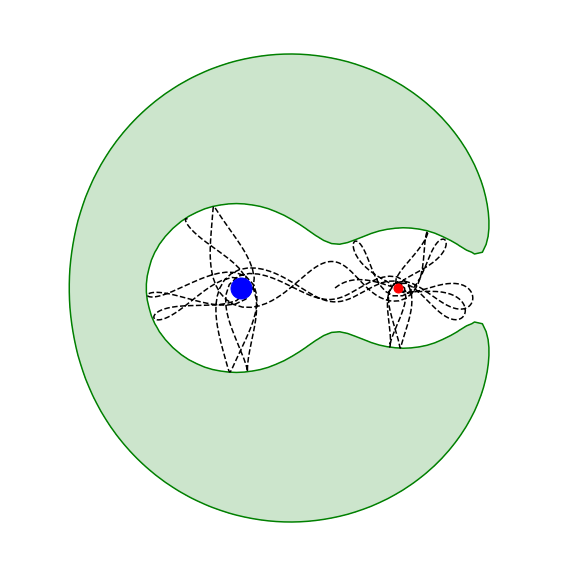
\includegraphics[width=1.0\textwidth]{\portada}}
  \end{center}%
}

% WATERMARK
\usepackage{draftwatermark}
\SetWatermarkText{BORRADOR}
\SetWatermarkLightness{0.9}
\SetWatermarkScale{0.5}

% BABEL
\usepackage[spanish]{babel}
\addto\extrasspanish{%
  \def\subsectionautorefname{Sección}%
  \def\sectionautorefname{Sección}%
  \def\figureautorefname{Figura}%
  \def\tableautorefname{Tabla}%
  \def\chapterautorefname{Capítulo}%
}



\title{\mytitle}

    
    
\author{\myauthor}

    

    % Pygments definitions
    
\makeatletter
\def\PY@reset{\let\PY@it=\relax \let\PY@bf=\relax%
    \let\PY@ul=\relax \let\PY@tc=\relax%
    \let\PY@bc=\relax \let\PY@ff=\relax}
\def\PY@tok#1{\csname PY@tok@#1\endcsname}
\def\PY@toks#1+{\ifx\relax#1\empty\else%
    \PY@tok{#1}\expandafter\PY@toks\fi}
\def\PY@do#1{\PY@bc{\PY@tc{\PY@ul{%
    \PY@it{\PY@bf{\PY@ff{#1}}}}}}}
\def\PY#1#2{\PY@reset\PY@toks#1+\relax+\PY@do{#2}}

\expandafter\def\csname PY@tok@w\endcsname{\def\PY@tc##1{\textcolor[rgb]{0.73,0.73,0.73}{##1}}}
\expandafter\def\csname PY@tok@c\endcsname{\let\PY@it=\textit\def\PY@tc##1{\textcolor[rgb]{0.25,0.50,0.50}{##1}}}
\expandafter\def\csname PY@tok@cp\endcsname{\def\PY@tc##1{\textcolor[rgb]{0.74,0.48,0.00}{##1}}}
\expandafter\def\csname PY@tok@k\endcsname{\let\PY@bf=\textbf\def\PY@tc##1{\textcolor[rgb]{0.00,0.50,0.00}{##1}}}
\expandafter\def\csname PY@tok@kp\endcsname{\def\PY@tc##1{\textcolor[rgb]{0.00,0.50,0.00}{##1}}}
\expandafter\def\csname PY@tok@kt\endcsname{\def\PY@tc##1{\textcolor[rgb]{0.69,0.00,0.25}{##1}}}
\expandafter\def\csname PY@tok@o\endcsname{\def\PY@tc##1{\textcolor[rgb]{0.40,0.40,0.40}{##1}}}
\expandafter\def\csname PY@tok@ow\endcsname{\let\PY@bf=\textbf\def\PY@tc##1{\textcolor[rgb]{0.67,0.13,1.00}{##1}}}
\expandafter\def\csname PY@tok@nb\endcsname{\def\PY@tc##1{\textcolor[rgb]{0.00,0.50,0.00}{##1}}}
\expandafter\def\csname PY@tok@nf\endcsname{\def\PY@tc##1{\textcolor[rgb]{0.00,0.00,1.00}{##1}}}
\expandafter\def\csname PY@tok@nc\endcsname{\let\PY@bf=\textbf\def\PY@tc##1{\textcolor[rgb]{0.00,0.00,1.00}{##1}}}
\expandafter\def\csname PY@tok@nn\endcsname{\let\PY@bf=\textbf\def\PY@tc##1{\textcolor[rgb]{0.00,0.00,1.00}{##1}}}
\expandafter\def\csname PY@tok@ne\endcsname{\let\PY@bf=\textbf\def\PY@tc##1{\textcolor[rgb]{0.82,0.25,0.23}{##1}}}
\expandafter\def\csname PY@tok@nv\endcsname{\def\PY@tc##1{\textcolor[rgb]{0.10,0.09,0.49}{##1}}}
\expandafter\def\csname PY@tok@no\endcsname{\def\PY@tc##1{\textcolor[rgb]{0.53,0.00,0.00}{##1}}}
\expandafter\def\csname PY@tok@nl\endcsname{\def\PY@tc##1{\textcolor[rgb]{0.63,0.63,0.00}{##1}}}
\expandafter\def\csname PY@tok@ni\endcsname{\let\PY@bf=\textbf\def\PY@tc##1{\textcolor[rgb]{0.60,0.60,0.60}{##1}}}
\expandafter\def\csname PY@tok@na\endcsname{\def\PY@tc##1{\textcolor[rgb]{0.49,0.56,0.16}{##1}}}
\expandafter\def\csname PY@tok@nt\endcsname{\let\PY@bf=\textbf\def\PY@tc##1{\textcolor[rgb]{0.00,0.50,0.00}{##1}}}
\expandafter\def\csname PY@tok@nd\endcsname{\def\PY@tc##1{\textcolor[rgb]{0.67,0.13,1.00}{##1}}}
\expandafter\def\csname PY@tok@s\endcsname{\def\PY@tc##1{\textcolor[rgb]{0.73,0.13,0.13}{##1}}}
\expandafter\def\csname PY@tok@sd\endcsname{\let\PY@it=\textit\def\PY@tc##1{\textcolor[rgb]{0.73,0.13,0.13}{##1}}}
\expandafter\def\csname PY@tok@si\endcsname{\let\PY@bf=\textbf\def\PY@tc##1{\textcolor[rgb]{0.73,0.40,0.53}{##1}}}
\expandafter\def\csname PY@tok@se\endcsname{\let\PY@bf=\textbf\def\PY@tc##1{\textcolor[rgb]{0.73,0.40,0.13}{##1}}}
\expandafter\def\csname PY@tok@sr\endcsname{\def\PY@tc##1{\textcolor[rgb]{0.73,0.40,0.53}{##1}}}
\expandafter\def\csname PY@tok@ss\endcsname{\def\PY@tc##1{\textcolor[rgb]{0.10,0.09,0.49}{##1}}}
\expandafter\def\csname PY@tok@sx\endcsname{\def\PY@tc##1{\textcolor[rgb]{0.00,0.50,0.00}{##1}}}
\expandafter\def\csname PY@tok@m\endcsname{\def\PY@tc##1{\textcolor[rgb]{0.40,0.40,0.40}{##1}}}
\expandafter\def\csname PY@tok@gh\endcsname{\let\PY@bf=\textbf\def\PY@tc##1{\textcolor[rgb]{0.00,0.00,0.50}{##1}}}
\expandafter\def\csname PY@tok@gu\endcsname{\let\PY@bf=\textbf\def\PY@tc##1{\textcolor[rgb]{0.50,0.00,0.50}{##1}}}
\expandafter\def\csname PY@tok@gd\endcsname{\def\PY@tc##1{\textcolor[rgb]{0.63,0.00,0.00}{##1}}}
\expandafter\def\csname PY@tok@gi\endcsname{\def\PY@tc##1{\textcolor[rgb]{0.00,0.63,0.00}{##1}}}
\expandafter\def\csname PY@tok@gr\endcsname{\def\PY@tc##1{\textcolor[rgb]{1.00,0.00,0.00}{##1}}}
\expandafter\def\csname PY@tok@ge\endcsname{\let\PY@it=\textit}
\expandafter\def\csname PY@tok@gs\endcsname{\let\PY@bf=\textbf}
\expandafter\def\csname PY@tok@gp\endcsname{\let\PY@bf=\textbf\def\PY@tc##1{\textcolor[rgb]{0.00,0.00,0.50}{##1}}}
\expandafter\def\csname PY@tok@go\endcsname{\def\PY@tc##1{\textcolor[rgb]{0.53,0.53,0.53}{##1}}}
\expandafter\def\csname PY@tok@gt\endcsname{\def\PY@tc##1{\textcolor[rgb]{0.00,0.27,0.87}{##1}}}
\expandafter\def\csname PY@tok@err\endcsname{\def\PY@bc##1{\setlength{\fboxsep}{0pt}\fcolorbox[rgb]{1.00,0.00,0.00}{1,1,1}{\strut ##1}}}
\expandafter\def\csname PY@tok@kc\endcsname{\let\PY@bf=\textbf\def\PY@tc##1{\textcolor[rgb]{0.00,0.50,0.00}{##1}}}
\expandafter\def\csname PY@tok@kd\endcsname{\let\PY@bf=\textbf\def\PY@tc##1{\textcolor[rgb]{0.00,0.50,0.00}{##1}}}
\expandafter\def\csname PY@tok@kn\endcsname{\let\PY@bf=\textbf\def\PY@tc##1{\textcolor[rgb]{0.00,0.50,0.00}{##1}}}
\expandafter\def\csname PY@tok@kr\endcsname{\let\PY@bf=\textbf\def\PY@tc##1{\textcolor[rgb]{0.00,0.50,0.00}{##1}}}
\expandafter\def\csname PY@tok@bp\endcsname{\def\PY@tc##1{\textcolor[rgb]{0.00,0.50,0.00}{##1}}}
\expandafter\def\csname PY@tok@fm\endcsname{\def\PY@tc##1{\textcolor[rgb]{0.00,0.00,1.00}{##1}}}
\expandafter\def\csname PY@tok@vc\endcsname{\def\PY@tc##1{\textcolor[rgb]{0.10,0.09,0.49}{##1}}}
\expandafter\def\csname PY@tok@vg\endcsname{\def\PY@tc##1{\textcolor[rgb]{0.10,0.09,0.49}{##1}}}
\expandafter\def\csname PY@tok@vi\endcsname{\def\PY@tc##1{\textcolor[rgb]{0.10,0.09,0.49}{##1}}}
\expandafter\def\csname PY@tok@vm\endcsname{\def\PY@tc##1{\textcolor[rgb]{0.10,0.09,0.49}{##1}}}
\expandafter\def\csname PY@tok@sa\endcsname{\def\PY@tc##1{\textcolor[rgb]{0.73,0.13,0.13}{##1}}}
\expandafter\def\csname PY@tok@sb\endcsname{\def\PY@tc##1{\textcolor[rgb]{0.73,0.13,0.13}{##1}}}
\expandafter\def\csname PY@tok@sc\endcsname{\def\PY@tc##1{\textcolor[rgb]{0.73,0.13,0.13}{##1}}}
\expandafter\def\csname PY@tok@dl\endcsname{\def\PY@tc##1{\textcolor[rgb]{0.73,0.13,0.13}{##1}}}
\expandafter\def\csname PY@tok@s2\endcsname{\def\PY@tc##1{\textcolor[rgb]{0.73,0.13,0.13}{##1}}}
\expandafter\def\csname PY@tok@sh\endcsname{\def\PY@tc##1{\textcolor[rgb]{0.73,0.13,0.13}{##1}}}
\expandafter\def\csname PY@tok@s1\endcsname{\def\PY@tc##1{\textcolor[rgb]{0.73,0.13,0.13}{##1}}}
\expandafter\def\csname PY@tok@mb\endcsname{\def\PY@tc##1{\textcolor[rgb]{0.40,0.40,0.40}{##1}}}
\expandafter\def\csname PY@tok@mf\endcsname{\def\PY@tc##1{\textcolor[rgb]{0.40,0.40,0.40}{##1}}}
\expandafter\def\csname PY@tok@mh\endcsname{\def\PY@tc##1{\textcolor[rgb]{0.40,0.40,0.40}{##1}}}
\expandafter\def\csname PY@tok@mi\endcsname{\def\PY@tc##1{\textcolor[rgb]{0.40,0.40,0.40}{##1}}}
\expandafter\def\csname PY@tok@il\endcsname{\def\PY@tc##1{\textcolor[rgb]{0.40,0.40,0.40}{##1}}}
\expandafter\def\csname PY@tok@mo\endcsname{\def\PY@tc##1{\textcolor[rgb]{0.40,0.40,0.40}{##1}}}
\expandafter\def\csname PY@tok@ch\endcsname{\let\PY@it=\textit\def\PY@tc##1{\textcolor[rgb]{0.25,0.50,0.50}{##1}}}
\expandafter\def\csname PY@tok@cm\endcsname{\let\PY@it=\textit\def\PY@tc##1{\textcolor[rgb]{0.25,0.50,0.50}{##1}}}
\expandafter\def\csname PY@tok@cpf\endcsname{\let\PY@it=\textit\def\PY@tc##1{\textcolor[rgb]{0.25,0.50,0.50}{##1}}}
\expandafter\def\csname PY@tok@c1\endcsname{\let\PY@it=\textit\def\PY@tc##1{\textcolor[rgb]{0.25,0.50,0.50}{##1}}}
\expandafter\def\csname PY@tok@cs\endcsname{\let\PY@it=\textit\def\PY@tc##1{\textcolor[rgb]{0.25,0.50,0.50}{##1}}}

\def\PYZbs{\char`\\}
\def\PYZus{\char`\_}
\def\PYZob{\char`\{}
\def\PYZcb{\char`\}}
\def\PYZca{\char`\^}
\def\PYZam{\char`\&}
\def\PYZlt{\char`\<}
\def\PYZgt{\char`\>}
\def\PYZsh{\char`\#}
\def\PYZpc{\char`\%}
\def\PYZdl{\char`\$}
\def\PYZhy{\char`\-}
\def\PYZsq{\char`\'}
\def\PYZdq{\char`\"}
\def\PYZti{\char`\~}
% for compatibility with earlier versions
\def\PYZat{@}
\def\PYZlb{[}
\def\PYZrb{]}
\makeatother


    % Exact colors from NB
    \definecolor{incolor}{rgb}{0.0, 0.0, 0.5}
    \definecolor{outcolor}{rgb}{0.545, 0.0, 0.0}



    
    % Prevent overflowing lines due to hard-to-break entities
    \sloppy 
    % Setup hyperref package
    \hypersetup{
      breaklinks=true,  % so long urls are correctly broken across lines
      colorlinks=true,
      urlcolor=urlcolor,
      linkcolor=linkcolor,
      citecolor=citecolor,
      }
    % Slightly bigger margins than the latex defaults
    
    \geometry{verbose,tmargin=1in,bmargin=1in,lmargin=1in,rmargin=1in}
    
    

\begin{document}
    
    
    
\maketitle

    
    
    \tableofcontents\listoffigures


    
\hypertarget{prefacio}{%
\chapter{Prefacio}\label{prefacio}}
\label{sec:00-1_Prefacio}
En 2019 celebramos el centenario de la histórica observación de un
eclipse total de Sol, liderada por \emph{Sir Arthur Eddington} y que
permitió la primera confirmación experimental de las predicciones de la
teoría general de la relatividad. El primer día de ese mismo año, una
nave espacial, la sonda \textbf{New Horizons}, sobrevoló el cuerpo
astronómico más remoto fotografiado por nuestra especie, el objeto
transneptuniano \textbf{(486958) Arrokoth}; la misma sonda, cinco años
antes, había pasado ``rozando'' la superficie de Plutón, enviándonos
imágenes inesperadas de un mundo sorprendente. Muy lejos de allí, y
también en 2019, dos naves espaciales, una japonesa, la sonda
\textbf{Hayabusa 2} y la otra estaudinense, \textbf{OSIRIS-REx},
transmitieron imágenes impactantes desde la superficie de dos pequeños
asteroides cercanos a la Tierra, cuerpos que visitaron con el objeto de
traer muestras a la Tierra. Lo que aprendamos de esas muestras podría
ayudarnos a evitar un impacto catastrófico futuro.

\begin{figure}[h]
\centering
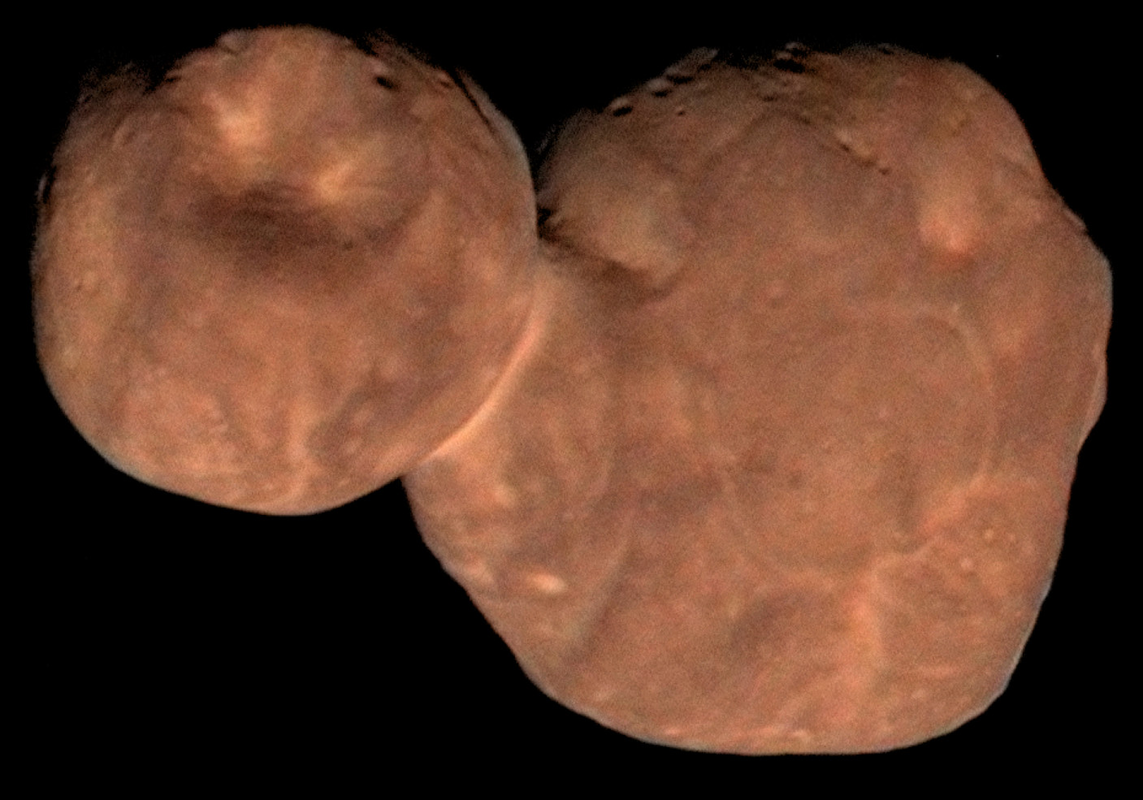
\includegraphics[width=0.7\textwidth]{./figures/horizontal_ultima_thule.png}
\caption{Imagen procesada de Arrokoth, el objeto transneptuniano
sobrevolado por la sonda New Horizons el 1 de enero 2019 (crédito:
NASA/Johns Hopkins University Applied Physics Laboratory/Southwest
Research Institute/Roman Tkachenko.)\label{fig:utlima_thule}}
\end{figure}

Todas estas hazañas de exploración y conocimiento fueron posibles, entre
otras, gracias a la \textbf{Mecánica Celeste}. Esta disciplina
científica, combinación asombrosa de astronomía, física y matemáticas,
comenzó con el trabajo teórico pionero de \emph{Johanes Kepler} a
principios de los 1600\footnote{En la \autoref{introduccion} haremos
  claridad sobre la nomenlatura usada en el libro para referirnos a los
  siglos y decenios.}; se estableció con la obra cumbre de \emph{Sir
Isaac Newton}, los \emph{Principios Matemáticos de la Filosofía Natural}
\cite{Newton1780Principia}, publicada a finales de los 1600; y alcanzó
su apogeo entre los 1700 y los 1800 con los trabajos de matemáticos y
astrónomos como \emph{Edmund Halley}, \emph{Leonhard Euler},
\emph{Pierre-Simon Laplace}, \emph{Joseph-Louis Lagrange}, \emph{William
Rowan Hamilton} y \emph{Henri Poincaré} (entre muchos otros que
mencionaremos en este libro).

Este libro presenta una visión panorámica de la \textbf{mecánica
celeste} y en general de la \textbf{mecánica analítica} o
\textbf{mecánica clásica}, que se desarrollo de forma paralela a la
primera, inspirada, en muchos casos, por sus problemas. El texto esta
dirigido especialmente a quiénes, por su formación o trabajo, están
interesados en la aplicación de la mecánica celeste en astronomía o en
ingeniería aeroespacial. Su extensión, énfasis y nivel de profundidad lo
hace especialmente adecuado para \textbf{estudiantes de pregrado}
(licenciatura o bachillerato, dependiendo del país) de cualquier
programa científico o técnico, especialmente astronomía, física o
ingeniería aeroespacial. Su enfoque computacional, lo podría hacer,
además, útil como material de referencia para profesionales de estas
disciplinas.

\hypertarget{otro_libro}{%
\section{¿Otro libro de mecánica celeste?}\label{otro_libro}}

Al escribir este libro, no pretendo hacer un compendio exhaustivo de los
problemas de la Mecánica Celeste, que, durante más de 400 años de
historia se ha convertido en una disciplina científica basta y en
constante desarrollo.

Muchos textos en la materia han sido escritos desde los tiempos de
Newton, la mayoría en las últimas décadas. Algunos presentan detallados
y rigurosos desarrollos matemáticos. Otros están orientados
específicamente al Sistema Solar o al movimiento de satélites y
vehículos espaciales. Muchos más son buenos libros de texto, la mayoría
dirigidos a estudiantes de posgrado (la mecánica celeste es considerada
una línea de profundización, tanto en física como en astronomía.)
También se han escrito algunos libros divulgativos y al alcance de
aficionados.

La bibliografía de este libro recoge apenas una muestra de referencias
en la materia, que serán citados a lo largo de sus capítulos, y que, de
antemano, invito a los lectores a explorar con curiosidad para no
quedarse con la punta de el inmenso \emph{iceberg} que apenas alcanzará
a asomarse en estas páginas.

Siendo este el caso ¿para qué escribir un libro más de mecánica celeste?
Existen dos razones fundamentales que me motivaron a emprender esta
aventura.

La primera es que, como mencione antes, la mayoría de los libros de
mecánica celeste están dirigidos a estudiantes con una formación media o
avanzada en matemáticas, mecánica newtoniana y mecánica analítica. Como
se acostumbra decir, tienen un nivel de posgrado. En contraste, el
número de textos al ``alcance'' de estudiantes de los primeros años
universitarios, no es muy grande. Escribo este libro para contribuir a
enriquecer precisamente ese ``nicho''.

Podría argumentarse que la mecánica celeste, como aplicación específica
de la mecánica, es un tema especializado y de allí que sus textos estén
dirigidos a estudiantes más avanzados. Sin embargo, la importancia de
esta disciplina en la historia de la astronomía y de la física, así como
su potencial para describir fenómenos fascinantes, desde el movimiento
de planetas y naves espaciales, hasta la colisión de agujeros negros,
hace de la mecánica celeste un medio educativo excelente para introducir
conceptos teóricos en física y astronomía, que, sin un contexto y
motivación apropiado, son difíciles de digerir.

Un buen libro de mecánica celeste o mecánica analítica, sin importar su
nivel, debería poder ser estudiado por cualquier estudiante, incluso de
pregrado. Esa ha sido la premisa en muchos centros académicos. Pero la
realidad es más compleja. Como cualquier profesor sensible sabe, para
valorar realmente los logros intelectuales del pasado, entender las
motivaciones que llevaron a los padres de una disciplina a introducir
hipótesis o formular las leyes de la misma, se necesita experiencia
académica. Experiencia que la mayoría de los estudiantes de pregrado no
tienen. No es solo un problema de nivel matemático, es también un
problema de falta de exposición a la ciencia.

Este libro, pretende ser un buen \emph{primer} libro de mecánica
celeste, pero también de mecánica analítica, como explicaremos más
adelante. Un primer escalón para abordar, ya con experiencia, libros más
avanzados.

\hypertarget{celeste_analitica}{%
\section{Mecánica celeste y mecánica
analítica}\label{celeste_analitica}}

La segunda razón, y la original para mi como profesor del
\textbf{pregrado de Astronomía en la Universidad de Antioquia}, fue la
necesidad de escribir un texto de mecánica celeste que permitierá además
una formación en los principios y métodos de la mecánica analítica
(mecánica teórica o mecánica clásica). Esos principios y métodos son
instrumentales en la formulación de la mecánica cuántica y lo son además
en versiones modernas de otras áreas de la física clásica, como la
relatividad, la electrodinámica e incluso la óptica. La mecánica
analítica es indispensable entonces en la formación de cualquier
estudiante de ciencias físicas.

En la inmensa mayoría de los textos clásicos de mecánica celeste, los
resultados se derivan usando, casi exclusivamente, los métodos de lo que
llamaremos aquí el \textbf{formalismo vectorial o geométrico de la
mecánica}. En este formalismo (originalmente introducido por Newton y
desarrollado posteriormente por Euler) las fuerzas juegan el papel
central en la descripción de la dinámica (\emph{dime cuánto te halan y
te diré cómo te mueves}.)

Desde los trabajos pioneros de matemáticos y ``físicos'' de los 1700 y
1800, tales como \emph{Alambert}, \emph{Lagrange}, \emph{Hamilton} y
\emph{Jacobi}, se hizo evidente que algunos problemas complejos de
mecánica celeste podían abordarse usando un \textbf{formalismo analítico
o escalar de la mecánica}. En este formalismo, los sistemas se describen
usando \emph{funciones} tales como el \emph{Lagrangiano} o el
\emph{Hamiltoniano}, que contienen toda la información relevante del
sistema, sus restricciones y simetrías (\emph{dime cuál es tu
hamiltoniano y no solo te diré para dónde vas sino también cómo eres}.)

Un caso ilustrativo, muy popular y reciente, de como el formalismo
analítico de la mecánica es aplicado hoy, de forma generalizada, en
mecánica celeste, es la ``predicción'' de un nuevo planeta en el Sistema
Solar, más allá del cinturón de Kuiper, cuya existencia, a la fecha, no
se ha confirmado, ni rechazado \cite{Batygin2016Planet9}. Este trabajo
también es la punta de un inmenso ``iceberg'' de literatura científica
en mecánica celeste en la que el formalismo analítico es protagonista.

Más allá entonces de la necesidad práctica de juntar a la mecánica
celeste y a la mecánica analítica en un mismo texto, de modo que sirva a
estudiantes de programas académicos como astronomía o ingeniería
aeroespacial, este libro presenta este particular ``matrimonio'' entre
dos disciplinas clásicas de la astronomía y la física como lo que es:
una relación estrecha entre dos cuerpos de conocimiento inseparables.

\hypertarget{celeste_era_informacion}{%
\section{Mecánica celeste en la era de la
información}\label{celeste_era_informacion}}

Un ingrediente adicional hace a este libro diferente. Me refiero al
enfásis especial que daremos a los algoritmos de la mecánica celeste a
través de todo el libro.

Es un hecho reconocido que la complejidad de muchos problemas de
mecánica celeste, en particular aquellos con un interés práctico tales
como el diseño de trayectorias de vehículos espaciales, la predicción de
la posición precisa de asteroides y cometas que pueden amenazar nuestro
planeta o la predicción a largo plazo de la posición de los cuerpos del
sistema solar y otros sistema planetarios, ha exigido, casi desde los
tiempos de Kepler, el desarrollo y aplicación de métodos numéricos y,
más recientemente, su implementación en calculadores y computadores.

En este sentido, la relación de la mecánica celeste con
\emph{algoritmos} de toda clase, no es comparable con la relación,
principalmente utilitaria, que tienen la mayoría de las área de la
física con la computación. Podría decirse, que hoy, es casi impensable
saber de mecánica celeste, sin estar familiarizado también con sus
algoritmos.

Pensando en esto, todo el contenido del libro ha sido elaborado usando
\emph{libretas} o \emph{notebooks} del
\hreffoot{https://jupyter.org}{Proyecto \texttt{Jupyter}}. Estas libretas
pueden ser obtenidas y usadas por el lector para interactuar con y
modificar los algoritmos (el material electrónico esta disponible en el
\hreffoot{http://seap-udea.org/MecanicaCeleste_Zuluaga}{sitio en línea} del
libro). Estos medios tecnológicos permiten además aprovechar gráficos
interactivos y animaciones para entender mejor conceptos que pueden ser
difíciles.

En la versión impresa, los algoritmos se presentarán en cajas especiales
de texto como esta:

    \begin{code}{}{}\begin{Verbatim}[fontsize=\small,commandchars=\\\{\}]
\PY{k+kn}{import} \PY{n+nn}{math}
\PY{n}{e}\PY{o}{=}\PY{l+m+mf}{0.3}
\PY{n}{M}\PY{o}{=}\PY{l+m+mf}{0.5}
\PY{n}{E}\PY{o}{=}\PY{n}{M}
\PY{n}{Eo}\PY{o}{=}\PY{l+m+mi}{2}\PY{o}{*}\PY{n}{M}
\PY{k}{while} \PY{n+nb}{abs}\PY{p}{(}\PY{n}{E}\PY{o}{\PYZhy{}}\PY{n}{Eo}\PY{p}{)}\PY{o}{\PYZgt{}}\PY{l+m+mf}{0.01}\PY{p}{:}
    \PY{n}{Eo}\PY{o}{=}\PY{n}{E}
    \PY{n}{E}\PY{o}{=}\PY{n}{M}\PY{o}{+}\PY{n}{e}\PY{o}{*}\PY{n}{math}\PY{o}{.}\PY{n}{sin}\PY{p}{(}\PY{n}{E}\PY{p}{)}
\PY{n+nb}{print}\PY{p}{(}\PY{l+s+s2}{\PYZdq{}}\PY{l+s+s2}{E = }\PY{l+s+s2}{\PYZdq{}}\PY{p}{,}\PY{n}{E}\PY{p}{)}
\end{Verbatim}

%%

\end{code}

    \begin{Verbatim}[fontsize=\small,commandchars=\\\{\}]
E =  0.6886561865220447
\end{Verbatim}

¿Puede el lector adivinar qué hace este algoritmo?. Si no lo hace,
espero que sepa en qué lenguaje de programación está escrito.

\hypertarget{celeste_python}{%
\section{Mecánica celeste en Python}\label{celeste_python}}

Es casi imposible escribir un libro con algoritmos sin comprometerse con
un lenguaje de programación específico (especialmente si queremos que
los algoritmos funcionen.) En el caso de esta edición del libro, el
lenguaje elegido es \texttt{Python}.

Esta siempre será una apuesta arriesgada. Aunque la mecánica celeste y
sus algoritmos no pasarán de ``moda'', los lenguajes de programación
``van y vienen''. Es un hecho (poco reconocido) que cientos de libros
científicos acumulan polvo por haber comprometido su contenido con
lenguajes de programación que hoy no son tan populares (\texttt{BASIC} o
\texttt{Pascal} por ejemplo).

No sabemos si \texttt{Python} y este libro sufrirán a la larga la misma
suerte. Pero hay tres hechos que \emph{sugieren} que la popularidad de
este lenguaje podría durar más de lo esperado (o al menos esa es mi
esperanza).

El primero es que su sintaxis es muy similar a la del ``lenguaje
natural''. Considere, por ejemplo, el algoritmo presentado antes (que ya
lo sabe, esta escrito en \texttt{Python}) o el siguiente algoritmo, aún
más simple:

    \begin{code}{}{}\begin{Verbatim}[fontsize=\small,commandchars=\\\{\}]
\PY{k+kn}{from} \PY{n+nn}{math} \PY{k}{import} \PY{n}{pi}
\PY{k}{for} \PY{n}{n} \PY{o+ow}{in} \PY{n+nb}{range}\PY{p}{(}\PY{l+m+mi}{1}\PY{p}{,}\PY{l+m+mi}{5}\PY{p}{)}\PY{p}{:}
    \PY{n+nb}{print}\PY{p}{(}\PY{l+s+s2}{\PYZdq{}}\PY{l+s+s2}{pi a la}\PY{l+s+s2}{\PYZdq{}}\PY{p}{,}\PY{n}{n}\PY{p}{,}\PY{l+s+s2}{\PYZdq{}}\PY{l+s+s2}{es}\PY{l+s+s2}{\PYZdq{}}\PY{p}{,}\PY{n}{pi}\PY{o}{*}\PY{o}{*}\PY{n}{n}\PY{p}{)}
\end{Verbatim}

%%

\end{code}

    \begin{Verbatim}[fontsize=\small,commandchars=\\\{\}]
pi a la 1 es 3.141592653589793
pi a la 2 es 9.869604401089358
pi a la 3 es 31.006276680299816
pi a la 4 es 97.40909103400242
\end{Verbatim}

Es difícil que estos algoritmos se escriban de manera tan natural en
casi cualquier otro lenguaje de programación popular en ciencia
(\texttt{C}, \texttt{FORTRAN} o \texttt{Java}) como se pueden escribir
en \texttt{Python}. Este hecho, no solo facilita el aprendizaje del
lenguaje, sino también la legibilidad de los algoritmos.

El segundo hecho que demuestra el promisorio futuro de \texttt{Python}
como lenguaje de la computación científica, es la creciente cantidad
paquetes, en todas las disciplinas de la ciencia y la técnica, que se
escriben permanentemente en este lenguaje y que están disponibles en
\hreffoot{https://pypi.org/project/IPy}{repositorios públicos}. Además,
herramientas informáticas muy conocidas (bibliotecas de rutinas, bases
de datos, sistemas de información, etc.) escritas originalmente en otros
lenguajes, han sido ahora traducidas a \texttt{Python}
(\emph{pythonizadas} si quieren) con el único propósito de que puedan
ser usadas por la creciente comunidad de desarrolladores en este
lenguaje.

\texttt{Python} se esta convirtiendo, y esta es una conjetura mía, en
depositario de décadas de experiencia en ciencia computacional.
¿Cambiará esta tendencia pronto? Lo dudo (o al menos así lo espero, por
el bien de este libro).

Una última razón, pero no por ello, menos importante, para elegir
\texttt{Python} como el idioma oficial de los algoritmos en este libro
es la existencia de una biblioteca gráfica, robusta y bien documentada,
escrita para este lenguaje. Me refiero por supuesto a
\hreffoot{https://matplotlib.org/}{\texttt{matplotlib}}.

Con la excepción de paquetes científicos que incluyen avanzadas
facilidades de graficación, tales como \texttt{Mathematica},
\texttt{Matlab}, o \texttt{IDL} (todos ellos sujetos a algún tipo de
pago), la mayoría de los lenguajes de programación dependen, a veces, de
complejas bibliotecas gráficas o programas de terceros para hacer, hasta
los más sencillos gráficos.

En \texttt{Python}, hacer un gráfico elemental, es tan simple como
escribir:
%%HIDE%%
    \begin{code}{Algoritmo}{code:1_Prefacio_1}\begin{Verbatim}[fontsize=\small,commandchars=\\\{\}]
\PY{k+kn}{from} \PY{n+nn}{matplotlib}\PY{n+nn}{.}\PY{n+nn}{pyplot} \PY{k}{import} \PY{n}{plot}
\PY{n}{plot}\PY{p}{(}\PY{p}{[}\PY{l+m+mi}{1}\PY{p}{,}\PY{l+m+mi}{2}\PY{p}{,}\PY{l+m+mi}{3}\PY{p}{,}\PY{l+m+mi}{4}\PY{p}{]}\PY{p}{,}\PY{p}{[}\PY{l+m+mi}{1}\PY{p}{,}\PY{l+m+mi}{4}\PY{p}{,}\PY{l+m+mi}{9}\PY{p}{,}\PY{l+m+mi}{16}\PY{p}{]}\PY{p}{)}\PY{p}{;}
\end{Verbatim}

%%

\tcblower
\footnotesize
\em ver Figura \ref{fig:code:1_Prefacio_1}
\end{code}

    \begin{center}

\begin{figure}[ht!]
\centering
    \adjustimage{max size={0.8\linewidth}{0.8\paperheight}}{combined_files/combined_23_0.png}
\caption{Figura correspondiente al código \ref{code:1_Prefacio_1}.\label{fig:code:1_Prefacio_1}}
\end{figure}

    \end{center}
%{ \hspace*{\fill} \\}
    
\hypertarget{celeste_spice}{%
\section{\texorpdfstring{Mecánica celeste con
\texttt{SPICE}}{Mecánica celeste con SPICE}}\label{celeste_spice}}

Con el temor de haberlos aburrido ya suficiente con este largo prefacio,
no puedo dejar de mencionar aquí, una última herramienta que será
protagonista en este libro. Se trata de \texttt{SPICE}, una aplicación
desarrollado para la \hreffoot{https://naif.jpl.nasa.gov/naif/}{\emph{NASA's
Navigation and Ancillary Information Facility (NAIF)}}.

\texttt{SPICE} es un sistema de informacióm de uso libre, formado
basicamente por una biblioteca de rutinas para realizar cálculos en
mecánica celeste y de datos (\emph{kernels}) que permiten, usando esas
mismas rutinas, la determinación de la posición y orientación precisa
(pasada y futura) de muchos cuerpos del Sistema Solar y de algunos
vehículos espaciales lanzados por nuestra especie.

Esta herramienta ha cobrado, en años recientes, una popularidad
significativa en la comunidad académica. Sus rutinas y \emph{kernels}
están detrás de algunas de los servicios en línea más populares de NASA,
tales como el sistema
\hreffoot{https://ssd.jpl.nasa.gov/horizons.cgi}{\emph{NASA Horizons}}, que
permite, a través de distintas interfaces, calcular la posición pasada y
futura de cuerpos del sistema solar y naves espaciales; o del simulador
\hreffoot{https://eyes.nasa.gov/}{\emph{NASA's Eyes}} que ofrece vistas en
tiempo real de la posición de los cuerpos del sistema solar y de
misiones espaciales de la agencia espacial estadounidense.

En este libro usaremos las rutinas y \emph{kernels} de \texttt{SPICE} (a
través de la biblioteca
\hreffoot{https://spiceypy.readthedocs.io/en/master}{\texttt{spiceypy}},
desarrollada en \texttt{Python}) para ilustrar conceptos, desarrollar
ejemplos y resolver problemas que, de otro modo, implicarían un gran
esfuerzo algorítmico (el objetivo será no \emph{reinventar la rueda
redonda}.)

Al hacerlo, además, el lector, sin importar su nivel, se familiarizará
con una herramienta que usan astrónomos e ingenieros aeroespaciales para
resolver problemas reales de mecánica celeste. ¡De la teoría a la
acción!

De la misma manera como nos preguntamos en el caso de \texttt{Python},
nos formulamos la siguienete pregunta: ¿podría \texttt{SPICE}
desaparecer o, mejor, ser reemplazada por un sistema diferente en los
próximos años? No podemos asegurarlo, pero la cantidad de herramientas
que hoy dependen de este sistema de información, hace dificil suponer
que podría cambiar radicalmente en el futuro inmediato.

Un último aspecto hace de \texttt{SPICE} una opción muy estable para los
propósitos de un libro de texto. La biblioteca de rutinas asociada con
el sistema esta disponible para un amplio conjunto de lenguajes de
programación diferentes a \texttt{Python}. Familiarizarse con las
rutinas y \emph{kernels} de \texttt{SPICE} aquí, será suficiente para
que pueda usarlo con lenguajes como \texttt{C/C++}, \texttt{FORTRAN} e
\texttt{IDL}.

A continuación, y a modo de ilustración, presento un algoritmo, escrito
con \texttt{SPICE}, para calcular la distancia de la Tierra al Sol
durante el eclipse total de Sol del 29 de maryo de 1919 en el que se
obtuvieron las primeras evidencias empíricas de la relatividad general y
con el que abrimos este prefacio. Naturalmente, este algoritmo es mucho
más complejo (y menos natural) que los que escribí antes, pero ilustra
el poder de esta herramienta para obtener resultados interesantes con
muy poco esfuerzo computacional.

    \begin{code}{}{}\begin{Verbatim}[fontsize=\small,commandchars=\\\{\}]
\PY{k+kn}{import} \PY{n+nn}{spiceypy} \PY{k}{as} \PY{n+nn}{spy}
\PY{n}{spy}\PY{o}{.}\PY{n}{furnsh}\PY{p}{(}\PY{l+s+s1}{\PYZsq{}}\PY{l+s+s1}{pymcel/data/naif0012.tls}\PY{l+s+s1}{\PYZsq{}}\PY{p}{)}
\PY{n}{spy}\PY{o}{.}\PY{n}{furnsh}\PY{p}{(}\PY{l+s+s1}{\PYZsq{}}\PY{l+s+s1}{pymcel/data/de430.bsp}\PY{l+s+s1}{\PYZsq{}}\PY{p}{)}
\PY{n}{et}\PY{o}{=}\PY{n}{spy}\PY{o}{.}\PY{n}{str2et}\PY{p}{(}\PY{l+s+s2}{\PYZdq{}}\PY{l+s+s2}{05/29/1919 09:08:00 UTC\PYZhy{}3}\PY{l+s+s2}{\PYZdq{}}\PY{p}{)}
\PY{n}{sol}\PY{p}{,}\PY{n}{tluz}\PY{o}{=}\PY{n}{spy}\PY{o}{.}\PY{n}{spkgeo}\PY{p}{(}\PY{l+m+mi}{10}\PY{p}{,}\PY{n}{et}\PY{p}{,}\PY{l+s+s2}{\PYZdq{}}\PY{l+s+s2}{J2000}\PY{l+s+s2}{\PYZdq{}}\PY{p}{,}\PY{l+m+mi}{0}\PY{p}{)}
\PY{n}{tierra}\PY{p}{,}\PY{n}{tluz}\PY{o}{=}\PY{n}{spy}\PY{o}{.}\PY{n}{spkgeo}\PY{p}{(}\PY{l+m+mi}{399}\PY{p}{,}\PY{n}{et}\PY{p}{,}\PY{l+s+s2}{\PYZdq{}}\PY{l+s+s2}{J2000}\PY{l+s+s2}{\PYZdq{}}\PY{p}{,}\PY{l+m+mi}{0}\PY{p}{)}
\PY{n}{distancia}\PY{o}{=}\PY{n}{spy}\PY{o}{.}\PY{n}{vnorm}\PY{p}{(}\PY{n}{tierra}\PY{o}{\PYZhy{}}\PY{n}{sol}\PY{p}{)}
\end{Verbatim}

%%

\end{code}
\vspace{-1em}

%%hidecode


    \begin{Verbatim}[fontsize=\small,commandchars=\\\{\}]
Distancia Tierra-Sol durante el eclipse de 1919: 151649284 km
\end{Verbatim}

\hypertarget{libro_distinto}{%
\section{¿Qué hace distinto a este libro?: un
decálogo}\label{libro_distinto}}

Para resumir, enumero a continuación las 10 cosas que hacen de este un
libro distinto de los muchos que se han escrito en casi 400 años de
historia de la mecánica celeste. Este decálogo, como la mayor parte de
este prefacio, es, además de una descripción abreviada de las
características únicas del libro, una lista de razones que justifican la
existencia de un libro más en el ``basto océano'' de literatura en la
materia.

\begin{enumerate}
\def\labelenumi{\arabic{enumi}.}
\item
  ¿Ya les mencione que es un libro para estudiantes de pregrado? Para
  entender su contenido no es necesario haber visto previamente un curso
  de mecánica analítica o matemáticas especiales. Solo se necesita una
  fundamentación mínima en geometría, cálculo y física.
\item
  El libro ha sido escrito, en la medida de las posibilidades, para ser
  autocontenido. Todo lo que un lector necesita saber de los fundamentos
  matemáticos (geometría, cálculo vectorial, ecuaciones diferenciales),
  los fundamentos físicos (mecánica newtoniana), astronómicos o de
  computación, ha sido incluído en los capítulos o en apéndices. Esto
  hace del libro, un texto que puede ser leído o estudiado por personas
  ajenas a la disciplina, incluso por aficionados.
\item
  El libro utiliza, como la mayoría de los textos en el área, el
  \emph{formalismo geométrico y vectorial} de la mecánica para presentar
  y desarrollar los problemas centrales de la mecánica celeste. Pero
  también introduce el \emph{formalismo analítico} (mecánica analítica o
  mecánica clásica) y lo aplica a la mecánica celeste. Es por tanto un
  libro de mecánica celeste y al mismo tiempo uno de mecánica analítica.
\item
  El libro no profundiza en todos los temas de la mecánica celeste o la
  mecánica analítica como lo hacen textos más avanzados. Pero, para un
  estudiante de pregrado, esta podría ser su primera lectura antes de
  abordar esos textos.
\item
  El texto hace un enfasis especial en los algoritmos de la mecánica
  celeste, que implementa usando códigos en \texttt{Python}, gráficas en
  \texttt{matplotlib} y, en ocasiones, usando algunas de las rutinas y
  datos del sistema \texttt{SPICE} de NASA.
\item
  Todo el libro esta disponible como \emph{notebooks} de
  \texttt{Jupyter} que pueden ser modificados por el lector o ejecutados
  durante una clase (¡es un libro para enseñar!) Los \emph{notebooks}
  contienen gráficos interactivos y animaciones que ilustran conceptos
  que pueden resultar difíciles.
\item
  El libro no requiere conocimientos previos de programación en
  \texttt{Python} (aunque tenerlos puede ser muy útil.) En realidad, el
  libro podría utilizarse como una manera de aprender el lenguaje en
  contexto, algo que es difícil de conseguir en libros dedicados
  específicamente a la enseñanza de la programación.
\item
  Los temas no se desarrollan en el orden en el que aparecieron en la
  historia: problema de los dos cuerpos \(\rightarrow\) teoría de
  perturbaciones \(\rightarrow\) problema de los tres cuerpos
  \(\rightarrow\) mecánica celeste relativistica, etc. He preferido
  presentarlos como me hubiera gustado conocerlos desde el principio,
  siguiendo un orden más lógico y un poco atemporal. Esta es la manera
  en la que, creo, un viajero en el tiempo, que retrocediera a 1700, se
  lo explicaría a un sorprendido Newton.
\item
  A pesar de lo anterior, la historia es importante en el libro. A
  través de los capítulos y en recuadros especiales he incluído anédotas
  y biografías que permitirán hacerse a una idea del contexto en el que
  surgieron las principales ideas de la mecánica celeste y la mecánica
  analítica y de los personajes, hombres y mujeres, que las concibieron.
\item
  Por muchas de las razones descritas arriba podría decirse que este es
  un libro ``moderno'' de mecánica celeste. uno que en lugar de ocuparse
  de llenar cientos de páginas con sesudos y rigurosos desarrollos
  matemáticos, le apunta directamente a dar vida a esas ideas y a
  ofrecer las herramientas prácticas para su aplicación.
\end{enumerate}

\textbf{El autor}

\emph{Febrero 19 de 2020}



\hypertarget{agradecimientos}{%
\chapter{Agradecimientos}\label{agradecimientos}}
\label{sec:01-2_Agradecimientos}
Así como no hay \emph{vacas esféricas en el vacío}, tampoco existen los
\emph{autores cilíndricos que escriben aislados}. La elaboración de este
libro ha sido determinada y afectada por una multitud de factores y
personas a los que no puedo dejar de mencionar.

En primer lugar, quiero agradecer a todos \textbf{los estudiantes del
pregrado de astronomía} que tomaron el curso de Mecánica Celeste durante
los años en los que elaboré las notas que sirvieron de base para este
libro. Agradezco su paciencia y sus preguntas en clase que me ayudaron a
enriquecer el texto, concentrarme en puntos difíciles y escoger mejor
los temas más interesantes. También fue de gran valor los errores que me
ayudaron a detectar en las primeras versiones de las \emph{libretas} de
\texttt{Jupyter} que son la base del texto. Entre ellos, quiero resaltar
a \textbf{Andrés Gómez}, quien fue mas lejos aún al revisar críticamente
el contenido de algunas \emph{libretas} como lo haría un colega o un
editor. Adicionalmente, sus impecables soluciones de los problemas
inspiraron una parte del material que he incluido en esta edición del
libro.

Una buena parte de la primera versión de las notas del curso fue
\textbf{transcrita a LaTeX} por el hoy Astrónomo \textbf{Bayron
Portilla} (en ese entonces mi tallerista del curso). En un momento dado,
nos propusimos, incluso, escribir juntos el libro. Sin embargo, nuestras
ocupaciones fueron dilatando el proyecto hasta que decidí emprender este
proyecto en solitario y partiendo de las \emph{libreta} de
\texttt{Jupyter} que elabore posteriormente. Aún así, reconozco y
agradezco el esfuerzo que hizo Bayron en esas primeras notas, en las que
además exploramos las mejores maneras de organizar los temas del curso.
Tal vez en el futuro retome con él algunas de esas notas iniciales con
miras a un texto avanzado en la materia donde podamos, por ejemplo,
abordar los tópicos que se quedaron por fuera de este libro. En el mismo
sentido debo también agradecer al Doctor \textbf{Andrés Pérez}, ahora un
exitoso astrónomo, quién en sus años como estudiante se ofreció también
a transcribir en limpio muchas de mis notas de tablero. El documento
resultante que nunca logramos editar apropiadamente todavía lo uso como
material de consulta en mis clases. Gracias Andrés por tu dedicación
durante esos meses a poner en limpio el sucio de mis tableros.

Estoy también en deuda con \textbf{Miguel Vásquez}, el mejor de los
talleristas que he tenido en mi carrera como profesor (ahora es un
Astrónomo). Miguel realizó una juiciosa tarea de búsqueda de problemas,
transcripción de los mismos al formato de \texttt{Jupyter} y, más
importante, preparación en el mismo formato de su solución. Todo,
mientras mantenía una estrecha relación con los estudiantes (mucho mejor
que la mía como profesor, debo admitir) que le permitió entender sus
necesidades, evaluar y ajustar el grado de dificultad de los problemas y
recoger correcciones y sugerencias a las notas. \textbf{Muchos
problemas} incluídos en este libro se basan en el trabajo original de
Miguel al que debo hacer un sentido reconocimiento aquí.

Agradezco también a los maestros que me motivaron a estudiar física
teórica durante el pregrado y el posgrado, muy a pesar de mi
monocromática pasión por la astronomía. Esto me permitió entender,
apreciar y abordar mejor los aspectos teóricos de la mecánica celeste.
En particular, mis agradecimientos van para los profesores
\textbf{Lorenzo de la Torre}, \textbf{Alonso Sepúlveda}, \textbf{Jorge
Mahecha}, \textbf{William Ponce} y \textbf{Boris Rodríguez}. A través de
sus propios manuscritos, conocí (y espero haber aprendido con el
ejemplo) el ``arte'' de escribir libros de texto. El estilo, profundidad
y cuidado de sus \textbf{notas de clase, libros publicados e inéditos},
han sido imitados sistemáticamente en este libro.

Agradezco a la \textbf{Universidad de Antioquia} y en particular a las
autoridades del \textbf{Instituto de Física} y la \textbf{Facultad de
Ciencias Exactas y Naturales}, por otorgarme el beneficio de un año
sabático, durante el cuál pude, entre otras cosas maravillosas, escribir
la primera versión completa de este libro. Mi reconocimiento y
agradecimiento además para los \textbf{profesores del pregrado de
Astronomía}, en especial a mi \emph{parcero} Pablo Cuartas, que recibió
mi carga académica y de investigación durante ese año en el que estuve
escribiendo.

Finalmente, pero no menos importante, quiero agradecer a mi familia,
\textbf{Olga y Sofía}. A ellas les toco la peor parte; es decir,
soportarme un año entero en la casa, escribiendo en piyamas (o mejor
hablando solo, por yo no escribo sino que hablo con el computador) y
prestándoles, a veces, menos atención de la que les presto incluso en
situaciones normales. Este libro esta dedicado a ellas.



\hypertarget{introduccion}{%
\chapter{Introducción}\label{introduccion}}
\label{sec:02-3_Introduccion}
\hypertarget{organizacion_libro}{%
\section{¿Cómo se organiza este libro?}\label{organizacion_libro}}

Como mencionamos en la \autoref{libro_distinto}, una de las cosas
hace a este libro diferente de otros textos de mecánica celeste, es la
manera y el orden particular en el que se desarrollan los temas. El
libro esta dividido en tres grandes partes:

\begin{itemize}
\tightlist
\item
  Los fundamentos matemáticos y físicos.
\item
  Mecánica celeste usando vectores y geometría (formalismo vectorial de
  la mecánica).
\item
  Mecánica analítica (formalismo lagrangiano y hamiltoniano) y su
  aplicación en mecánica celeste.
\end{itemize}

En los siguiente párrafos encontrarán una síntesis \emph{narrada} del
libro; algo así como una \emph{tabla de contenido comentada} que le
permitirá al lector, no solo orientarse en el texto, sino también
entender la manera como se encadenan cada una de sus partes.

Y es que todo libro debería contar una \emph{historia}. En los textos
académicos, lamentablemente, esa ``vocación'' narrativa parece perderse
en medio de figuras, teoremas y algoritmos. Esta sección puede ser
entonces entendida, como un esfuerzo para esbozar la \emph{historia} que
se hila a través de sus capítulos.

\begin{itemize}
\item
  \textbf{Parte 1: Fundamentos matemáticos y físicos}. Antes de
  comenzar, respasaremos algunos temas de matemáticas y de física
  necesarios para estudiar mecánica celeste. Si bien el lector debería
  estar familiarizado con la mayoría de estos temas, he decidido incluir
  este capítulo no solo para hacer al texto autocontenido, sino también
  con el propósito de compilar resultados útiles, definiciones y
  algorítmos, en el formato y notación del texto, que se usarán en
  capítulos posteriores.

  \begin{itemize}
  \item
    \textbf{\autoref{fundamentos}}. Algunos consideran a la mecánica
    celeste un área de las matemáticas aplicadas. En ella confluyen
    técnicas matemáticas de todos los orígenes. Por esta misma razón
    para comprender incluso los aspectos más básicos de la teoría es
    necesario contar con una sólida fundamentación matemática. Por
    razones de espacio no podemos cubrir todos los temás relevantes en
    esta sección, pero nos hemos concentrado en dos de particular
    importancia en todo el texto:

    \begin{itemize}
    \item
      \textbf{\autoref{cónicas}}: El cálculo infinitesimal fue
      \emph{descubierto} por Isaac Newton a finales de los 1600 (y más
      tarde descubierto independientemente también por Gottfried
      Leibniz), inspirado, en parte en problemas mecánicos. Estos
      métodos matemáticos permitieron a Newton, sus contemporáneos y
      suscesores resolver los complicados problemas de la mecánica
      celeste que inauguraron la disciplina. Por la misma razón es
      indispensable que el lector repase las cantidades y resultados
      centrales de este método analítico, que es justamente el tema de
      esta sección. Al hacerlo aprovecharemos además para recoger
      algunas definiciones y resultados importantes de la geometría y el
      cálculo de vectores, los elementos básicos de la teoría de
      ecuaciones diferenciales y del más \emph{exótico} cálculo de
      variaciones. Ninguno de los apartes de este capítulo cumple
      funciones \emph{decorativas} o es completamente prescindible. A
      pesar de parecer una sección ajeno al libro, un material que
      debería dejarse solo a los autores expertos en el tema, en
      realidad todos los resultados expuestos aquí serán usados en el
      resto de capítulos.
    \item
      \textbf{\autoref{cónicas}}: En esta sección nos concentraremos
      en repasar (o presentar) las propiedades de las figuras cónicas,
      su definición y descripción geométrica más general, así como su
      descripción algebraica. Las cónicas juegan un papel central en la
      mecánica celeste y estar familiarizado con ellas, permitirá
      resolver más fácilmente problemas físicos relativamente complejos.
      Estudiaremos esta familia particular de curvas, tanto en el plano,
      como en el espacio de tres dimensiones. Con este propósito,
      introduciremos aquí el tema de las rotaciones en dos y tres
      dimensiones (ángulos de Euler) que son usados con frecuencia en la
      mecánica celeste pero también en la mecánica analítica.
    \end{itemize}
  \item
    \textbf{\autoref{mecanica}}. Es casi imposible presentar la
    mecánica celeste y menos aún la mecánica analítica, sin repasar
    primero las definiciones, postulados y proposiciones de la mecánica
    básica, o mecánica newtoniana, como se la llama comunmente. Este
    capítulo esta justamente dedicado a presentar el que llamaremos
    \textbf{formalismo vectorial o geométrico} de la mecánica,
    desarrollado a partir de las ideas mismas de Newton pero
    enriquecidas significativamente por sus sucesores en los siguientes
    dos siglos. Si bien, de nuevo, este podría parecer un tema
    \emph{elemental} para tratar en otro libro, la manera en la que se
    presenta aquí es particularmente única. He tratado de formular las
    ideas de siempre en un orden más moderno y en algunos casos poco
    ortodoxo. No pretendo con ello producir \emph{ninguna revolución},
    pero al hacerlo, la presentación de los tema centrales del libro se
    hace más natural. El capítulo se concentra en la mecánica de
    partículas y sistemas de partículas, sin ocuparse de otros temas
    interesantes de la mecánica, la dinámica de cuerpos rígidos o de
    fluídos, que no serán aplicados en el resto del texto.
  \end{itemize}
\end{itemize}

\begin{itemize}
\item
  \textbf{Parte 2: El formalismo vectorial de la mecánica celeste}. Como
  veremos a lo largo del libro, la mecánica puede ser presentada usandos
  dos enfoques matemáticas o \emph{formalismos} diferentes. En esta
  parte del curso nos concentraremos en la formulación geométrica o
  vectorial de la mecánica celeste, la más popular y la que uso
  originalmente Newton en sus \emph{Principia} y que fue desarrollada
  posteiormente por sus sucesores.

  \begin{itemize}
  \item
    \textbf{\autoref{problema_ncuerpos}}. A diferencia de la mayoría
    de los textos en mecánica celeste, en este libro comenzamos por
    abordar y estudiar con algún detalle, el más general de los
    problemas de esta disciplina: el problema de los N cuerpos. En este
    problema, el reto consiste en predecir la posición y velocidad de
    muchos cuerpos que interactúan gravitacionalmente. Si bien el
    problema de los N cuerpos fue posiblemente el último de los grandes
    problemas de mecánica celeste en ser formulado y abordado
    rigurosamente en la historia, su presentación temprana en este
    libro, permitirá introducir resultados y métodos que serán de
    utilidad para el resto del texto. De particular interés será la
    introducción en este capítulo de los algoritmos para resolver
    numéricamente el problema. Estos algoritmos y algunas herramientas
    computacionales relacionadas, serán muy importante en el resto del
    texto, para comparar y validar resultados de modelos analíticos. Se
    presentará también aquí el concepto de integrales de movimiento o
    \emph{cuadraturas}, uno de los métodos usados clásicamente para
    extraer información sobre un sistema dinámico sin resolverlo
    completamente. Este método será usado regularmente en los demás
    capítulos.
  \item
    \textbf{\autoref{problema_dos_cuerpos}}. Una de las
    idealizaciones más conocidas de la mecánica celeste es aquella que
    consiste en suponer que cuando dos cuerpos astronómicos interactúan
    gravitacionalmente, el efecto del resto del Universo es
    completamente despreciable. Naturalmente, no existe ningún sistema
    astronómico real que cumpla cabalmente estas condición. Todos los
    sistemas del universo, en sentido estricto, son sistemas de N
    cuerpos. En este capítulo mostraremos, a través de experimentos
    numéricos y ejemplos astronómicos reales, que la mayoría de los
    sistemas astronómicos se pueden analizar dinámicamente como
    \emph{sistemas de N cuerpos jerárquicos}, es decir, sistemas en los
    que las partículas se agrupan por pares (pares de partículas, pares
    de pares, etc.) que se perturban mutuamente. El problema de los dos
    cuerpos no es, sin embargo, el destino final de la mecánica celeste,
    sino su punto de partida. Es un resultado útil para estudiar
    sistemas mucho más complejos. Resolveremos en este capítulo el
    problema de los dos cuerpos usando el método de las cuadraturas
    (primeras integrales de movimiento) introducido en el capítulo
    anterior. Demostraremos que el movimiento relativo de dos cuerpos se
    realiza sobre una cónica y desarrollaremos en detalle las relaciones
    entre las propiedades geométricas de esa cónica y las propiedades
    dinámicas del sistema. Resolveremos también, usando métodos
    geométricos primero y después métodos del cálculo, el denominado
    problema de los dos cuerpos en el tiempo, que conducirá a la famosa
    ecuación de Kepler.
  \item
    \textbf{\autoref{problema_tres_cuerpos}}. A pesar del poder que
    la teoría desarrollada en el capítulo anterior tiene para describir
    el movimiento de muchos sistemas astronómicos, existen situaciones
    que escapan a una descripción \emph{kepleriana} del movimiento
    orbital (incluso, una que incluye perturbaciones). El caso de la
    Luna, el de algunos cometas perturbados por Júpiter y el de
    vehículos espaciales modernos, son especialmente significativos. En
    este capítulo abordaremos, inicialmente, el problema general de los
    tres cuerpos, es decir, aquel en el que la dinámica no es
    jerarquica. A diferencia del problema de los dos cuerpos, no se
    conoce una solución general en términos de funciones analíticas al
    problema de los tres cuerpos. Una versión restringida de este
    problema, a saber el \emph{problema circular restringido de tres
    cuerpos} (\emph{CRTBP} por su sigla en inglés), tiene propiedades
    teóricas que han resultado de interés en la descripción de sistemas
    astronómicos reales. Estudiaremos aquí en detalle el CRTBP, su
    descripción dinámica y cinemática, tanto en sistemas inerciales como
    no inerciales. Introduciremos algoritmos para la solución numérica
    del problema en el sistema rotante. Encontraremos su constante de
    movimiento, la \emph{constante de Jacobi} y una aproximación
    astronómica en términos de elementos orbitales, el \emph{parámetro
    de Tisserand}. Deduciremos las propiedades y visualizaremos las
    denominadas \emph{regiones de exclusión} y \emph{curvas de cero
    velocidad} (conceptos interesantes que permiten, si no predecir
    dónde estarán los cuerpos, al menos, donde no estarán). Finalmente
    se deducirán las propiedades de los \emph{puntos de equilibrio de
    Lagrange} y algunas aplicaciones astronómicas y en mecánica orbital
    del problema.
  \end{itemize}
\end{itemize}

\begin{itemize}
\item
  \textbf{Parte 3: El formalismo analítico de la mecánica.} En esta
  parte del libro, introduciremos el \emph{formalismo analítico de la
  mecánica} y su aplicación en la solución de problemas de mecánica
  celeste. El formalismo analítico tiene una importancia central en la
  física que trasciende a la mecánica celeste (se usa por ejemplo para
  estudiar la dinámica de cuerpos rígidos y sistemas oscilantes, el caos
  en sistemas dinámicos, la mecánica relativista, el electromagnetismo,
  la teoría de campos clásica y la mecánica cuántica). Si bien pocas
  aplicaciones del formalismo, distintas a la mecánica celeste, se
  desarrollara en este texto (como si sucede en algunos textos avanzados
  de mecánica clásica) los fundamentos teóricos presentados en esta
  parte le permitiran al lector abordar el estudio de esas otras
  disciplinas en textos específicos de mecánica analítico o en textos
  más avanzados.

  \begin{itemize}
  \item
    \textbf{\autoref{formalismo_lagrangiano}}. En este capítulo se
    introducen los principios y teoremas centrales del formalismo
    analítico de la mecánica, en particular los principios de
    Alambert-Lagrange y de Hamilton. Haremos aquí, un especial énfasis
    en las motivaciones teóricas que llevaron a matemáticos y físicos de
    los 1700 a introducir este formalismo (un tema en el que los textos
    más avanzados de mecánica clásica, apenas si consideran.) Se
    introducirá aquí la función lagrangiana, las ecuaciones de Lagrange
    y, a través de la aplicación del cálculo variacional, se deduciran
    las ecuaciones generales de Euler-Lagrange (que tienen una
    aplicación amplia en muchas áreas de la física). Como un elemento
    novedoso se presentarán en este capítulo algunos algoritmos
    aplicados al formalismo lagrangiano, y en particular a la
    comprensión mejor del principio de Hamilton y los métodos del
    cálculo variacional. Con los elementos básicos del formalismo
    lagrangiano a la mano, procedermos a aplicarlo en la solución de
    problemas concretos en mecánica celeste. Para ello presentaremos,
    primero, resultados importantes sobre la relación entre las
    simetrías de la función lagrangiana y las cantidades conservadas en
    el movimiento (teorema de Noether). A partir de allí, procederemos
    de forma similar a como lo hicimos con el formalismo vectorial, a
    resolver el problema general de los N cuerpos y el de los dos
    cuerpos. Deduciremos el lagrangiano de los N cuerpos y de sus
    simetrías obtendremos las cantidades conservadas en el sistema. Pero
    ¿de qué sirve deducir los mismos resultados que ya habíamos visto en
    el capítulo correspondiente de la segunda parte?. Usaremos lo que
    sabemos de mecánica celeste para ilustrar el poder del formalismo
    lagrangiano frente al formalismo vectorial. Posteriormente,
    abordaremos el problema de los dos cuerpos usando el formalismo
    lagrangiano. En este caso, a diferencia del problema de los N
    cuerpos, tendremos una novedad. En lugar de restringirnos al caso de
    la gravitación Newtoniano, estudiaremos aquí el problema más general
    de sistemas de dos cuerpos sometidos a fuerzas centrales con un
    potencial generalizado. Los resultados obtenidos aquí, tendrán un
    rango más amplio de aplicación. Podrán por ejemplo usarse para
    estudiar la física de sólidos, moléculas y átomos, pero también la
    mecánica celeste postnewtoniana. Estudiaremos, en este contexto, el
    problema de fuerzas centrales reducido a una dimensión, el potencial
    efectivo (y las correspondientes zonas de exclusión). Para el caso
    del potencial newtoniano deduciremos la denominada ecuación de la
    forma orbital y resolveremos el problema de los dos cuerpos a partir
    de ella. Para el caso de un potencial general, pero no muy distinto
    del potencial Newtoniano, estudiaremos el denominado \emph{avance
    del perihelio} uno de los resultados teóricos de la mecánicaceleste
    que a la larga serían de la mayor importancia histórica al ofrecer
    las primeras evidencias de la validez de la teoría general de la
    relatividad.
  \item
    \textbf{\autoref{formalismo_hamiltoniano}}. En este capítulo
    abordamos el más general (y poderoso) formalismo analítico de la
    mecánica: el formalismo Hamiltoniano. Después de discutir las
    motivación para la introducción de este formalismo (motivaciones de
    naturaleza principalmente geométrica), deduciremos de forma
    heurística las ecuaciones canónicas (de primer orden) de Hamilton;
    introduciremos la función Hamiltoniana y demostraremos su
    equivalencia con las ecuaciones (de segundo orden) de
    Euler-Lagrange. Ilustraremos el poder del formalismo y la
    descripción de los sistemas en el denominado \emph{espacio de fase};
    para ello nos valdremos inicialmente de sistemas dinámicos simples
    (péndulos y bloques), como hicimos en el primer capítulo de esta
    parte. Posteriormente abordaremos (sin el detalle en el que lo
    hicimos en el caso del formalismo Lagrangiano y por las obvias
    analogías entre los dos formalismos) el tema de las simetrías y las
    cantidades conservadas, e introduciremos los útiles \emph{corchetes
    de Poisson}, como herramienta matemática para estudiar dichas
    simetrías. Escribiremos los hamiltonianos del problema general de
    los N cuerpos, el del problema de los dos cuerpos y el del problema
    circular restringido de los tres cuerpos, y redescubriremos, usando
    los elementos de este nuevo formalismo, las propiedades ya conocidas
    de estos sistemas. Una de las aplicaciones más poderosas del
    formalismo Hamiltoniano, se consigue al aprovechar las simetrías de
    los sistemas gravitacionales, para, a través de transformaciones de
    \emph{coordenadas} en el espacio de fase, escribir formas
    simplificadas de los Hamiltonianos. Estas formas simplificadas,
    además, permiten aplicar de forma más directa la teoría de
    perturbaciones y así estudiar sistemas muy complejos (un tema que no
    esta incluído en este libro.) En este capítulo introduciremos,
    primero, el tema de las transformaciones canónicas, que son
    transformaciones de coordenadas en el espacio de fase que mantienen
    la \emph{estructura hamiltoniana} de los sistemas (es decir, que
    hacen que los sistemas sigan siendo descritos con las ecuaciones
    canónicas). Nos concentraremos, especialmente en el formalismo de la
    función generatriz de las transformaciones canónicas. A
    continuación, aplicando la teoría de transformaciones canónicas
    presentaremos el método de Hamilton-Jacobi que permite, entre otras
    cosas, encontrar sistemas de coordenadas que simplifican
    significativamente la descripción de ciertos sistemas físicos. En
    particular utilizaremos este formalismo para deducir, en el problema
    de los dos cuerpos, el Hamiltoniano del sistema en términos de
    elementos orbitales; en particular, en términos de funciones
    específicas de esos elementos orbitales, que hacen lo más simple
    posible el hamiltoniano del sistema. El resultado más importante de
    este capítulo será la deducción de las denominadas \emph{variables
    de Dalaunay} que son de gran utilidad y poder en la mecánica celeste
    moderna y posiblemente el punto de partida de algunos textos de
    mecánica celeste avanzados.
  \end{itemize}
\end{itemize}

Todos los capítulos hasta aquí contarán con un conjunto completo de
preguntas, ejercicios y problemas, que permitiran al lector poner a
prueba los conocimientos adquiridos y las habilidades desarrolladas,
pero también, descubrir como estas ideas, métodos y herramientas, se
aplican en otras situaciones específicas.

\hypertarget{como_usar_libro}{%
\section{¿Cómo usar este libro?}\label{como_usar_libro}}

Este libro puede ser utilizado de tres formas diferentes:

\begin{enumerate}
\def\labelenumi{\arabic{enumi}.}
\item
  Como un texto para el \emph{autoaprendizaje} de la mecánica celeste y
  la mecánica analítica. Estudiantes y profesionales de muchas
  disciplinas, se pueden valer de él para tener su primer acercarmiento
  a estas disciplinas.
\item
  Como el texto guía de un primer curso de mecánica celeste y de
  mecánica analítica. El texto es una fuente de lecciones y problemas
  útiles para organizar un curso de pregrado.
\item
  Como material de referencia para estudaintes y profesionales. Muchas
  fórmulas, algoritmos, e incluso anécdotas e historias interesantes,
  podrían resultar útiles para quiénes ya tienen una formación en el
  área.
\end{enumerate}

Como \textbf{texto para el autoaprendizaje}, recomiendo \textbf{leer el
texto en su totalidad} incluyendo la primera parte de Fundamentación
matemática y física, en la que se encuentran algunos elementos teóricos
requeridos para el resto del libro.

Para quiénes tengan una formación avanzada en física, astronomía o
ingeniería, es posible que una buena fracción de los temas de esa
primera parte resulten sencillos y puedan obviarse. Sin embargo, aunque
los tópicos tratados allí parezcan conocidos (al menos nominalmente), su
tratamiento puede resultar novedoso. Si este es su caso, no deje de
echarle una mirada a esos primeros capítulos. En particular recomiendo
revisar, como mínimo, las secciones dedicadas a la solución numérica de
ecuaciones diferenciales, incluyendo las ecuaciones de movimiento en
mecánica newtoniana, los rudimentos de cálculo variacional y la dinámica
en sistemas rotantes, donde podrían encontrarse las diferencias más
significativas respecto a los textos canónicos de matemáticas y física,
y donde además se introducen herramientas algorítmicas que serán de uso
muy corriente en el resto del libro.

El uso ideal de este libro es como \textbf{texto guía} de un primer
curso de mecánica celeste y mecánica analítica. El libro fue escrito a
partir de la experiencia de más de 5 años ofreciendo el curso en el
pregrado de astronomía de la Universidad de Antioquia (en Medellín,
Colombia). Por la misma razón, la extensión y organización particular
del texto, se adapta de forma \emph{precisa} a las condiciones propias
de un curso universitario de un semestre de duración (cuatro meses
efectivos de lecciones.) El curso se ha ofrecido exitosamente a
estudiantes que han aprobado los cursos básicos de física (hasta el tema
de oscilaciones y ondas) y de cálculo (incluyendo cálculo vectorial y
ecuaciones diferenciales.)

Todos los capítulos del libro libro han sido dictados dentro del plazo
del curso. Sin embargo, dependiendo del nivel académico de los
estudiantes y de su independencia intelectual, el curso puede dictarse
sin incluir todos los temas de la primera parte.

Por mi experiencia dictando el curso, el repaso de los fundamentos puede
resultar extenso (como mínimo toma un mes que es justamente el período
en el que los estudiantes tienen una motivación y disposición mayor,
además de menos distracciones de otros cursos.) Sugeriría, entonces, que
de sacrificarse algunos temas de esa parte, se asigne la lectura
independiente a los estudiantes de los temas mejor conocidos y se evalúe
a través de la lista de problemas incluídos al final de los capítulos de
esa parte.

Como mencioné en la \autoref{celeste_era_informacion}, y se
detallará abajo, el libro fue escrito usando \emph{libretas de
\texttt{Jupyter}}, una por cada clase (a lo sumo se pueden dictar dos
clases con cada libreta). Es decir, el número de \emph{libretas} y su
organización puede ofrecer una idea del programa detallado de
actividades del curso o del plan de lecturas.

\hypertarget{celeste_libretas}{%
\section{\texorpdfstring{Mecánica celeste en
\emph{libretas}}{Mecánica celeste en libretas}}\label{celeste_libretas}}

El libro ha sido concebido, escrito y compilado enteramente usando
\emph{libretas} de \texttt{Jupyter}. Las libretas, que están disponibles
en la versión electrónica del texto, son archivos en un formato especial
(no son programa de \texttt{Python}, ni páginas web) que pueden ser
visualizadas y ejecutadas usando un navegador de Internet.

El uso de las libretas no es indispensable para entender el contenido
del libro, pero puede ofrecer una experiencia interactiva muy
enriquecedora y a veces acelerar el proceso de aprendizaje. El uso de
las libretas en clase puede, además, hacer más dinámica y amena la
interacción entre el profesor y los estudiantes.

Para hacer uso de las libretas se debe contar con un \textbf{computador
de escritorio} que use cualquier sistema operativo (\texttt{Windows},
\texttt{Linux} o \texttt{MacOS}). Por la misma razón, en caso de usarla,
recomiendo que el curso se desarrolle en una sala de computo. Para
ejecutar las libretas es necesario instalar primero el interprete y la
biblioteca base del lenguaje \texttt{Python}, un conjunto específico de
paquetes y el sistema \texttt{Jupyter}, además de varias de sus
extensiones (los detalles se presentan en la siguiente sección.)

La \hreffoot{http://seap-udea.org/MecanicaCeleste_Zuluaga}{versión en línea}
de este libro (páginas web), puede ser también una alternativa a las
libretas de \texttt{Jupyter}. Este formato tiene la ventaja que solo
requiere un dispositivo con conexión a Internet (de escritorio o móvil)
y puede manipularse en cualquier contexto. Aunque la versión web carece
de casi todas las características interactivas de las libretas de
\texttt{Jupyter}, en ella encontraran, además de todos los algoritmos y
gráficos, animaciones y otros elementos de \emph{hipertexto}.

\hypertarget{instalacion_libretas}{%
\subsection{Instalación de las libretas}\label{instalacion_libretas}}

Para aquellos que deseen aprovechar las libretas de \texttt{Jupyter}
como medio didáctico, se ofrece a continuación una guía básica de cómo
preparar un computador para ejecutarlas. Instrucciones adicionales
pueden encontrarse en la versión en línea del libro.

\begin{enumerate}
\def\labelenumi{\arabic{enumi}.}
\item
  \textbf{Instalación del lenguaje \texttt{Python} y las bibliotecas
  básicas del lenguaje.} El primer requisito para utilizar las libretas
  es instalar el interprete y las bibliotecas del sistema del lenguaje
  \texttt{Python}. Existen diversas maneras para hacerlo en cada sistema
  operativo y abundantes instrucciones en Internet. Mi recomendación es
  utilizar el sistema \hreffoot{https://www.anaconda.com}{\texttt{Anaconda}}
  que ofrece, en una plataforma integrada, los archivos del lenguaje
  \texttt{Python}, una amplia diversidad de paquetes científicos, el
  sistema \texttt{Jupyter} y todas las herramientas necesarias para la
  instalación de otros paquetes.
\item
  \textbf{Descargar las libretas.} Una vez haya instalado
  \texttt{Python} y \texttt{Jupyter}, puede descargar las libretas del
  libro los archivos adicionales requeridos por ellas del sitio web del
  libro. Para ello siga las instrucciones provistas allí.
\item
  \textbf{Ejecución de pruebas.} Para verificar si las libretas
  funcionan correctamente, una vez descargadas, busque y abra la libreta
  \texttt{Pruebas.ipynb}. Una vez abierta ejecute todas sus celdas
  (\texttt{Cell\ /\ Run\ all}). Si la ejecución se realiza completa, en
  la última celda aparecera un reporte completo con los resultados de la
  prueba. Si alguna de las prueba individuales falla, es posible que sea
  necesario instalar paquetes, datos adicionales y otras dependencias.
\item
  \textbf{Instalación de dependencias.} Para instalar todas las
  dependencias del libro abra la libreta \texttt{Instalacion.ipynb} y
  siga las instrucciones descritas allí.
\end{enumerate}

\hypertarget{idioma_notacion}{%
\section{Idioma y Notación}\label{idioma_notacion}}

\hypertarget{extranjerismos_pronunciacion}{%
\subsection{Palabras extranjeras y guía de
pronunciación}\label{extranjerismos_pronunciacion}}

El libro está escrito en español. Sin embargo, y como sucede con todas
las ciencias, habrán muchos apartes en los que es necesario introducir
términos técnicos y acrónimos procedentes de la lengua inglesa. En estos
casos las palabras y acrónimos se presentarán en itálica. Así por
ejemplo, al referirnos al problema matemático de resolver la ecuación de
movimiento de una partícula hablaremos del \emph{initial value problem}
o su acrónimo \emph{IVP}, en contraposición al \emph{boundary condition
problem}. Por otro lado en el \autoref{problema_tres_cuerpos}
estudiaremos el \emph{CRTBP} o \emph{circular restricted three body
problem}.

Muchos de los científicos (hombres y mujeres) que han contribuído con el
desarrollo de la mecánica celeste en sus cuatro siglos de historia,
tienen nombres y apellidos no hispanos. Su correcta pronunciación,
especialmente en el caso de autores franceses o de origen germano, es
difícil para quienes no hablamos las lenguas de esos pueblos.

Un caso notable, por ejemplo, es el nombre de la matemática alemana
\emph{Emmy Noether}. En castellano la mayoría pronunciaríamos ``emi
noeter'' o ``emmi neder'' (siguiendo la tradición inglesa con la que
estamos más familiarizados.) Como una primera guía para la correcta
pronunciación de estos nombres, a lo largo del libro presentaremos
``transliteraciones'' al castellano, indicando, entre comillas las
letras y palabras más cercanas que un hispanohablante podría usar. Así
por ejemplo ``niuton'' será la trasliteración fonética de Newton y la
pronunciación ``correcta'' (en alemán) del nombre de Emmy Noether, será
``emmi noutar''.

Para hacernos a una idea fonética más precisa nos apoyaremos a lo largo
del libro de la increíble colección compilada en
\hreffoot{http://forvo.com}{este sitio web} que ofrece pronunciaciones en
línea, en decenas de idiomas, de miles de nombres, palabras y frases.
Allí encontrará por ejemplo la pronunciación correcta, en su idioma
original del nombre
\hreffoot{https://es.forvo.com/search/Emmy\%20Noether/de/}{Emmy Noether}.

¿Es todo esto indispensable para entender la mecánica celeste o la
mecánica analítica?. Ciertamente no. Pero no solo de teoría vivimos los
humanos. La comunicación y socialización es central al proyecto
científico y es bueno entender y hacerse entender especialmente en
contextos internacionales.

\hypertarget{siglos_decadas}{%
\subsection{Siglos y décadas}\label{siglos_decadas}}

La historia de la mecánica celeste y análitica, así como la historia de
las áreas de la física y las matemáticas con las que se relaciona, es
fascinante. En el libro, como detallamaos en la próxima sección,
incluiremos abundantes referencias históricas sobre los personajes y los
momentos claves en el desarrollo de las ideas de la mecánica celeste.

Para referirnos a los siglos, sin embargo, nos desviaremos de las reglas
convencionales del español. Según esas reglas al período comprendido,
por ejemplo, entre 1701 y 1800, se lo llama el siglo XVIII. Para este
autor, la notación usando números romanos, si bien ampliamente aceptada,
es confusa y exige realizar operaciones mentales innecesarias (número
romano \(\rightarrow\) número indoarabigo \(\rightarrow\) restar uno
\(\rightarrow\) multiplicar por 100).

En los sucesivo para referirnos al período comprendido entre 1700 y 1799
(comenzando en el año cero y no en el año uno como dicta la regla)
hablaremos de \textbf{los 1700}. Así mismo el siglo XX será \textbf{los
1900} y así sucesivamente.

Dado que en las reglas establecidas del español, los 1900 hacen
referencia en realidad a la década entre 1901 y 1910, cuando queramos
refereirnos a un período de diez años siempre usaremos explícitamente la
palábra \textbf{década}: década de 1680, decada de 1960, etc.

No pretendó, con este acto de rebeldía \emph{idiomática}, cambiar el
castellano. Pero sí, al menos en lo que respecta a este libro, faciltar
la lectura de los períodos históricos.

\hypertarget{notacion}{%
\subsection{Notación matemática}\label{notacion}}

Todos los libros de ciencias físicas o matemáticas se ``casan'' con una
notación específica. La elección de la notación, no es sin embargo una
tarea sencilla, en tanto son muy comunes los casos de textos que en
virtud de su notación se hacen practicamente ilegibles aunque traten los
mismos temas o problemas de otros que usan notaciones más comunes.

Pensando justamente en esto, he tomado la decisión de utilizar, en la
medida de las posibilidades, la misma notación de algunos textos
clásicos de mecánica celeste, que se diferencia, a veces
significativamente, de la que utilizan libros de matemáticas e incluso
de física, con los que el lector puede estar familiarizado.

El lector encontrará los detalles específicos de la notación usada en el
libro en la \autoref{vectores_calculo}.

\hypertarget{elementos_no_textuales}{%
\section{Elementos no textuales}\label{elementos_no_textuales}}

Para facilitar la lectura del libro y hacer de la experiencia de leerlo
algo más agradable e incluso excitante, el texto contiene una serie de
elementos gráficos con los que debemos familiarizarnos.

\hypertarget{cajas_texto}{%
\subsection{Cajas de texto}\label{cajas_texto}}

Mucha información importante texto se presenta en \emph{cajas}
independientes al texto principal y cuyas características gráficas
resaltan del resto del documento. En particular existen 5 tipos de
cajas:

\begin{itemize}
\item
  \textbf{Resumen del capítulo}. Esta caja aparece normalmente al
  principio de cada capítulo y contiene una breve síntesis del mismo. No
  deje de leer este resumen para identificar los temas centrales de cada
  parte del libro. El profesor podría usar la información contenida allí
  para definir los objetivos específicos de la evaluación.
\item
  \textbf{Notas}. A veces es necesario desviarse un momento del hilo del
  texto para aclarar o ampliar asuntos relacionados con la notación, los
  paquetes y algorítmos utilizados, o simplemente llamar la atención
  sobre un asunto importante. A continuación se muestra un ejemplo de
  una \emph{caja de nota}.
\end{itemize}
\begin{box_note}{Nota}

\textbf{El lenguaje \emph{Markdown}.} La mayor parte del contenido
textual de este libro, ha sido escrito en las celdas de libretas de
\texttt{Jupyter} en un lenguaje de descripción de documentos conocido
como \emph{Markdown}. Puede explorar la sintaxis del lenguaje, o bien
desplegando el contenido de las \emph{celdas} de las libretas, o bien
consultando la abundante \hreffoot{https://markdown.es/}{documentación en
línea}.

\end{box_note}
\begin{itemize}
\tightlist
\item
  \textbf{Definiciones}. Muchas cantidades físicas y algunos conceptos
  claves requieren una definición rigurosa. Este es el rol justamente
  que juegan las \emph{cajas de definición}. A diferencia de las cajas
  de Resumen y Notas, las cajas de \emph{Definición} están numeradas
  (como las figuras o las ecuaciones), de modo que sea más fácil
  referirse a ellas.
\end{itemize}
\begin{box_definition}{Definición}{}

\textbf{Mecánica celeste.} Llamamos \emph{Mecánica Celeste} a la
disciplina científica que aplica las leyes de la mecánica para estudiar
el movimiento de cuerpos bajo la acción dominante de la gravedad. Dado
que solo en lugares lejanos a la superficie terrestre (normalmente fuera
de su atmósfera), la gravedad es la fuerza dominante, la mecánica
celeste normalmente describe el movimiento de cuerpos astronómicos
(desde partículas pequeñas, hielo o polvo interestelar, hasta planetas y
estrellas) y de vehículos espaciales. En este último caso se habla
normalmente de \emph{Mecánica orbital}.

\end{box_definition}
\begin{itemize}
\tightlist
\item
  \textbf{Teoremas, postulados y leyes}. Como las definiciones, en
  muchas ocasiones será indispensable separarnos un momento de una
  explicación para formular más rigurosamente un resultado, normalmente
  obtenido por razonamiento deductivo en el marco de una teoría
  (teoremas, lemas, colorarios) o por razonamiento inductivo a partir de
  la experiencia (leyes y postulados). Para hacerlo usaremos cajas de
  texto con una numeración independiente de aquella usada para las
  definiciones. Sin embargo, es importante aclarar que en el caso de los
  denominados \emph{teoremas} me he abstenido de usar sistemáticamente
  esta palabra en el encabezado de los respectivos recuadros. En su
  lugar he decidido imitar a algunos autores clásicos (en particular a
  Euclides) que usaban sistemáticamente la palabra \textbf{proposición}
  en lugar de teorema para referirse a afirmaciones demostrables. Es
  decir, en este libro, una \emph{proposición} será un resultado
  importante que puede estar o no demostrado en el texto. Al hacerlo
  quiero evitar posar aquí de matemático, una profesión a la que respeto
  profundamente\footnote{Decía el matemático húngaro Paul Eördos (``pol
    érdos'') que un \emph{matemático es una máquina para convertir café
    en teoremas}, una frase que aunque parece simplificar la naturaleza
    de los matemáticos, en realidad demuestra la importancia que tienen
    los teoremas para esta milenaria profesión.}. Aún así, cuando una
  \emph{proposición} dada corresponda a un teorema bien conocido, usaré
  la palabra teorema en el título interno de la caja. Las dos
  \emph{proposiciones} mostradas en las cajas a continuación ilustran
  estos conceptos.
\end{itemize}
\begin{box_theorem}{Proposición}{}

\textbf{Sistemas de referencia inerciales.} Si un sistema de referencia
\(O'\) se mueve con velocidad constante con respecto a un sistema de
referencia inercial \(O\), entonces \(O'\) es también un sistema de
referencia inercial.

\end{box_theorem}\begin{box_theorem}{Proposición}{}

\textbf{Teorema de Danelin.} Dada una esfera tangente a un cono y un
plano que corta el cono en un determinado ángulo, el punto de tangencia
de la esfera con el plano es uno de los focos de la cónica
correspondiente.

\end{box_theorem}
\begin{figure}[t!]
\centering
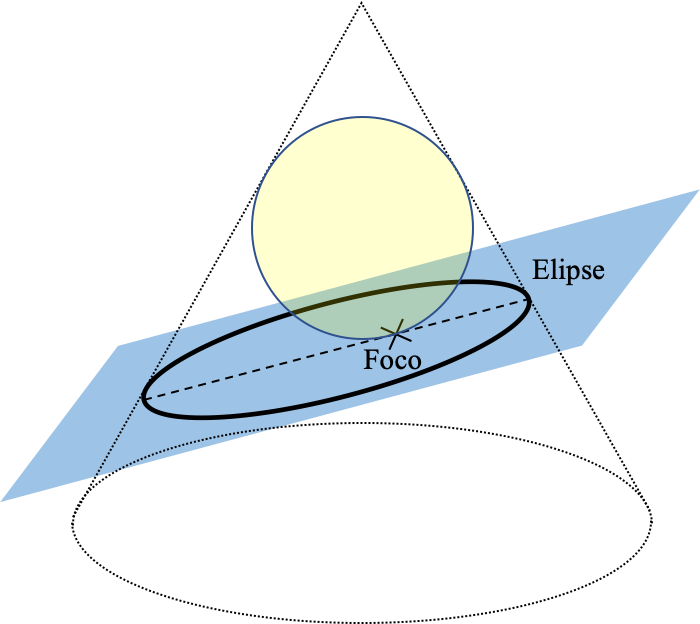
\includegraphics[width=0.5\textwidth]{./figures/square_teorema_danelin.png}
\caption{Ilustración esquemática del \emph{teorema de
Danelin}.\label{fig:teorema_danelin}}
\end{figure}

\begin{itemize}
\tightlist
\item
  \textbf{Un poco de historia}. Finalmente, pero no menos importante,
  están las anécdotas e historias que contaremos a lo largo de todo el
  libro. Como se menciono en el prefacio, la mecánica celeste tiene ya
  más de 400 años (aproximadamente 100 años más que la mecánica
  analítica) y cientos de libros y miles de artículos se han escrito en
  el tema. Es casi imposible hablar de mecánica celeste y analítica, sin
  mencionar de vez en cuando las historias que rodearon la invención de
  una técnica, la biografía de alguno de los grandes hombres y mujeres
  que concibieron las ideas contenidas en el libro o simplemente una
  anécdota curiosa relacionada con algún tema de interes.
\end{itemize}
\begin{box_history}{Un poco de historia}{t}{float}
\small

\textbf{¿Kepler o Newton?.} En el Prefacio daba a entender que la
mecánica celeste posiblemente había comenzado con los trabajos pioneros
de Johannes Kepler (ver \autoref{fig:kepler}). Otros autores van más
lejos y apuntan a los astrónomos de la antigüedad y la edad media,
especialmente indios, chinos, arabes y griegos, que desarrollaron
modelos complejos para la descripción del movimiento de los cuerpos
celestes. Los más conservadores apuntan a Sir Isaac Newton, quien
después de la publicación de su obra cumbre, los \emph{Principia}, sentó
las bases físicas, no solo para la mecánica celeste, sino también, en
general, para toda la mecánica.

La razón en este libro para escoger a Kepler, como el \emph{padre} de la
disciplina (y en general de la astronomía física) fueron sus
contribuciones decisivas y bastante bien conocidas para esclarecer
definitivamente la \emph{cinemática} del movimiento planetario. En
particular, el descubrimiento (o el enunciado matemático) de sus
conocidas \emph{leyes del movimiento planetario} representaron un cambio
cualitativo en el desarrollo de la teoría del movimiento planetario e
inspiraron en últimas el trabajo de Newton y sus contemporáneos.

Adicionalmente, y esto es aún más importante, Kepler fue uno de los
primeros astrónomos modernos (renacentistas europeos) en hacer
consideraciones teóricas sobre la causa del movimiento planetario, más
allá de ocuparse de su descripción, como lo hicieron la mayoría de los
astrónomos de la antigüedad y la edad media. Esto pone a Kepler, entre
esos astrónomos, como el primer \emph{astrofísico} de la historia.

\end{box_history}
\begin{figure}[t!]
\centering
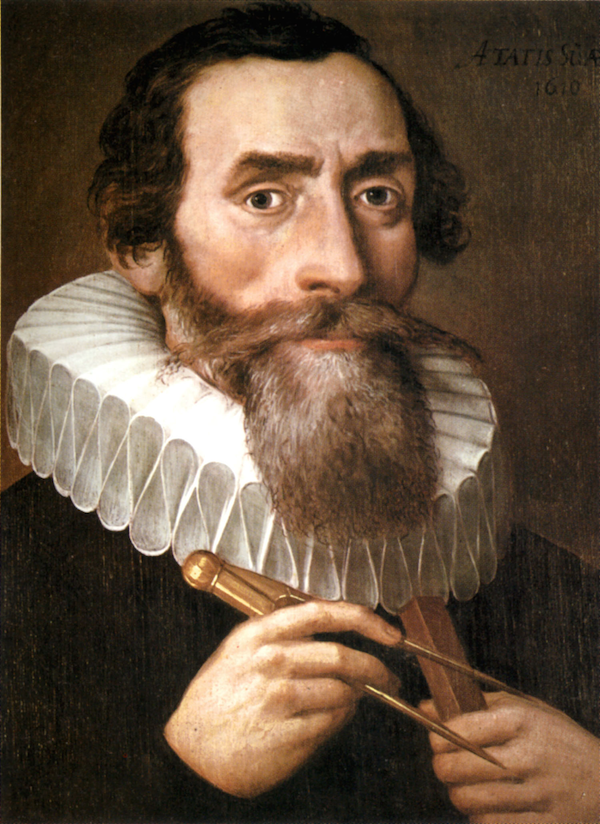
\includegraphics[width=0.5\textwidth]{./figures/vertical_kepler.png}
\caption{Retrato de Johanes Kepler, copia de un original de 1610 de
pintor desconocido y que se conserva en el monasterio Benedictino de
Kremsmünster (Alemania).\label{fig:kepler}}
\end{figure}

\hypertarget{algoritmos}{%
\subsection{Algoritmos}\label{algoritmos}}

Como he insistido hasta aquí, una de las novedades más importantes de
este libro es el énfasis que he querido dar a los \emph{algoritmos}. Por
algoritmo entenderemos aquí pequeños (o no tan pequeños) fragmentos de
código (\emph{code snippet} en inglés) que realizan tareas numéricas
específicas o son parte de un algoritmo mayor.

He evitado hablar de \emph{programas} o \emph{códigos} para resaltar el
hecho de que lo importante en ellos es la lógica de las operaciones y no
el lenguaje específico en el que están escritos. A pesar de este
esfuerzo por mantener el tema lo más general posible, es virtualmente
imposible escribir algoritmos que se puedan ejecutar realmente en las
libretas, sin recurrir a ciertas particularidades del lenguaje en el que
están descritos, \texttt{Python}.

Existen en general tres tipos de \emph{algoritmos} que encontraremos a
lo largo del texto. En primer lugar están los algoritmos más sencillos,
aquellos que ejecutan tareas básicas de preparación de datos para
algoritmos más complejos. Este es un caso de ellos:

    \begin{code}{}{}\begin{Verbatim}[fontsize=\small,commandchars=\\\{\}]
\PY{n}{a}\PY{o}{=}\PY{l+m+mi}{1}
\PY{n}{b}\PY{o}{=}\PY{o}{\PYZhy{}}\PY{l+m+mi}{1}
\PY{n}{c}\PY{o}{=}\PY{l+m+mi}{2}
\PY{n}{disc}\PY{o}{=}\PY{n}{b}\PY{o}{*}\PY{o}{*}\PY{l+m+mi}{2}\PY{o}{\PYZhy{}}\PY{l+m+mi}{4}\PY{o}{*}\PY{n}{a}\PY{o}{*}\PY{n}{c}
\end{Verbatim}

%%

\end{code}
\vspace{-1em}

%%hidecode


    \begin{Verbatim}[fontsize=\small,commandchars=\\\{\}]
Discriminante = -7.0
\end{Verbatim}

Muchos de estos algoritmos simples vienen seguidos del resultado más
importante de las operaciones que codifican. En el caso anterior se
muestra por ejemplo el valor del discriminante (el valor de la variable
\texttt{disc}). El algoritmo (o código) para producir ese resultado:

\begin{Shaded}
\begin{Highlighting}[]
  \BuiltInTok{print}\NormalTok{(}\SpecialStringTok{f"Discriminante = }\SpecialCharTok{\{}\NormalTok{disc}\SpecialCharTok{:.1f\}}\SpecialStringTok{"}\NormalTok{)}
\end{Highlighting}
\end{Shaded}

Pero este algoritmo (y la celda correspondiente) no se muestra en el
libro impreso para evitar la proliferación de código irrelevante.

Los algoritmos más complejos pueden, como las ecuaciones, estar
numerados:

    \begin{code}{Algoritmo}{code:rutina_discriminante}\begin{Verbatim}[fontsize=\small,commandchars=\\\{\}]
\PY{k}{def} \PY{n+nf}{calcula\PYZus{}discriminante}\PY{p}{(}\PY{n}{a}\PY{p}{,}\PY{n}{b}\PY{p}{,}\PY{n}{c}\PY{p}{)}\PY{p}{:}
    \PY{n}{disc}\PY{o}{=}\PY{n}{b}\PY{o}{*}\PY{o}{*}\PY{l+m+mi}{2}\PY{o}{\PYZhy{}}\PY{l+m+mi}{4}\PY{o}{*}\PY{n}{a}\PY{o}{*}\PY{n}{c}
    \PY{k}{return} \PY{n}{disc}
\end{Verbatim}

%%

\end{code}

En este caso, el algoritmo contiene una rutina o función, que podría ser
usada más adelante, incluso en un capítulo posterior. Todas las rutinas
como estas, hacen parte de un paquete incluído con las libretas llamado
\texttt{pymcel}. Para usar la rutina en el Alg.
(\ref{code:rutina_discriminante}) en otra parte del libro se usa:

    \begin{code}{}{}\begin{Verbatim}[fontsize=\small,commandchars=\\\{\}]
\PY{k+kn}{from} \PY{n+nn}{pymcel}\PY{n+nn}{.}\PY{n+nn}{export} \PY{k}{import} \PY{n}{calcula\PYZus{}discriminante}
\PY{n}{d}\PY{o}{=}\PY{n}{calcula\PYZus{}discriminante}\PY{p}{(}\PY{l+m+mi}{1}\PY{p}{,}\PY{l+m+mi}{2}\PY{p}{,}\PY{l+m+mi}{3}\PY{p}{)}
\end{Verbatim}

%%

\end{code}

Cualquier lenguaje de programación moderno depende de numerosas
bibliotecas en las que están codificados procedimientos de uso regular o
muy especializados. En todos los algoritmos presentados en el libro,
siempre que se use una rutina de una biblioteca externa, se presentará
el código que hace referencia a la biblioteca de forma explícita.
Consider por ejemplo este algoritmo:

    \begin{code}{Algoritmo}{code:raiz_polinomio}\begin{Verbatim}[fontsize=\small,commandchars=\\\{\}]
\PY{c+c1}{\PYZsh{}Coeficientes de un polinomio de segundo grado}
\PY{n}{a}\PY{o}{=}\PY{l+m+mi}{1}
\PY{n}{b}\PY{o}{=}\PY{l+m+mi}{3}
\PY{n}{c}\PY{o}{=}\PY{o}{\PYZhy{}}\PY{l+m+mi}{2}

\PY{c+c1}{\PYZsh{}Calcula discriminante}
\PY{k+kn}{from} \PY{n+nn}{pymcel}\PY{n+nn}{.}\PY{n+nn}{export} \PY{k}{import} \PY{n}{calcula\PYZus{}discriminante}
\PY{n}{d}\PY{o}{=}\PY{n}{calcula\PYZus{}discriminante}\PY{p}{(}\PY{n}{a}\PY{p}{,}\PY{n}{b}\PY{p}{,}\PY{n}{c}\PY{p}{)}

\PY{c+c1}{\PYZsh{}Calcula raices}
\PY{k}{if} \PY{n}{d}\PY{o}{\PYZgt{}}\PY{o}{=}\PY{l+m+mi}{0}\PY{p}{:}
    \PY{k+kn}{from} \PY{n+nn}{numpy} \PY{k}{import} \PY{n}{sqrt}
    \PY{n}{x1}\PY{o}{=}\PY{p}{(}\PY{o}{\PYZhy{}}\PY{n}{b}\PY{o}{+}\PY{n}{sqrt}\PY{p}{(}\PY{n}{d}\PY{p}{)}\PY{p}{)}\PY{o}{/}\PY{p}{(}\PY{l+m+mi}{2}\PY{o}{*}\PY{n}{a}\PY{p}{)}
    \PY{n}{x2}\PY{o}{=}\PY{p}{(}\PY{o}{\PYZhy{}}\PY{n}{b}\PY{o}{\PYZhy{}}\PY{n}{sqrt}\PY{p}{(}\PY{n}{d}\PY{p}{)}\PY{p}{)}\PY{o}{/}\PY{p}{(}\PY{l+m+mi}{2}\PY{o}{*}\PY{n}{a}\PY{p}{)}
\PY{k}{else}\PY{p}{:}
    \PY{n+nb}{print}\PY{p}{(}\PY{l+s+s2}{\PYZdq{}}\PY{l+s+s2}{El polinomio no tiene raices reales}\PY{l+s+s2}{\PYZdq{}}\PY{p}{)}
\end{Verbatim}

%%

\end{code}

En él hemos usado la rutina \texttt{sqrt} (raíz cuadrada) de la
biblioteca \texttt{NumPy} para calcular, en este caso, las raices de un
polinomio de segundo grado. Para ello, antes de la línea que usa la raíz
cuadrada hemos incluido la instrucción:

\begin{Shaded}
\begin{Highlighting}[]
\ImportTok{from}\NormalTok{ numpy }\ImportTok{import}\NormalTok{ sqrt}
\end{Highlighting}
\end{Shaded}

Aunque en los programas regurales, estas instrucciones se ponen al
principio, he decidido colocarlas lo más cerca posible al lugar donde se
usan de modo que los fragmentos de código funcionen fuera del contexto
del libro. El lector poco familiarizado con el lenguaje \texttt{Python}
puede hacer caso omiso a estas instrucciones, que nada le agregan a la
lógica de los algoritmos.
\begin{box_note}{Nota}

\textbf{las instrucciones \texttt{import} y la velocidad de los
programas.} Es importante advertir que en algunos algoritmos, usar
muchas instrucciones del timpo \texttt{import} entre las líneas de
código puede disminuir la velocidad del código. La recomendación general
es la de poner este tipo de instrucciones al principio del programa. Así
el Alg. (\ref{code:raiz_polinomio}) debería escribirse así:

\begin{Shaded}
\begin{Highlighting}[]
\ImportTok{from}\NormalTok{ pymcel.export }\ImportTok{import}\NormalTok{ calcula_discriminante}
\ImportTok{from}\NormalTok{ numpy }\ImportTok{import}\NormalTok{ sqrt}

\CommentTok{#Coeficientes de un polinomio de segundo grado}
\NormalTok{a}\OperatorTok{=}\DecValTok{1}
\NormalTok{b}\OperatorTok{=}\DecValTok{3}
\NormalTok{c}\OperatorTok{=-}\DecValTok{2}

\CommentTok{#Calcula discriminante}
\NormalTok{d}\OperatorTok{=}\NormalTok{calcula_discriminante(a,b,c)}

\CommentTok{#Calcula raices}
\ControlFlowTok{if}\NormalTok{ d}\OperatorTok{>=}\DecValTok{0}\NormalTok{:}
\NormalTok{    x1}\OperatorTok{=}\NormalTok{(}\OperatorTok{-}\NormalTok{b}\OperatorTok{+}\NormalTok{sqrt(d))}\OperatorTok{/}\NormalTok{(}\DecValTok{2}\OperatorTok{*}\NormalTok{a)}
\NormalTok{    x2}\OperatorTok{=}\NormalTok{(}\OperatorTok{-}\NormalTok{b}\OperatorTok{-}\NormalTok{sqrt(d))}\OperatorTok{/}\NormalTok{(}\DecValTok{2}\OperatorTok{*}\NormalTok{a)}
\ControlFlowTok{else}\NormalTok{:}
    \BuiltInTok{print}\NormalTok{(}\StringTok{"El polinomio no tiene raices reales"}\NormalTok{)}
\end{Highlighting}
\end{Shaded}

\end{box_note}
Otro tipo de algoritmos frecuentes son aquellos que dan como resultado
figuras o gráficos. Estos están entre los más interesantes y útiles,
aunque pueden ser complicados y causar algo de estupor para los menos
familiarizados con el lenguaje de programación. Les recomiendo a todos
poner especial atención en estos algoritmos, tratar de entenderlos e
imitarlos. Una buena parte de la ciencia que hacemos hoy día depende de
producir bonitos productos gráficos que ilustren de forma compacta
conceptos o resultados difíciles de describir de otra manera.

Todos los códigos que producen figuras están numerados. Así mismo los
gráficos que producen aparecen en el texto, incluso en el impreso, como
figuras independientes y numeradas. Por razones de eficiencia en el uso
del espacio, algunas de esos gráficos pueden estar en lugares lejanos de
la posición del código. Es por esto que en todos los algoritmos que
producen gráficos encontraran (en la parte inferior) una referencia a la
figura correspondiente.
%%HIDE%%
    \begin{code}{Algoritmo}{code:plot_sin}\begin{Verbatim}[fontsize=\small,commandchars=\\\{\}]
\PY{k+kn}{from} \PY{n+nn}{numpy} \PY{k}{import} \PY{n}{linspace}\PY{p}{,}\PY{n}{sin}\PY{p}{,}\PY{n}{pi}
\PY{n}{t}\PY{o}{=}\PY{n}{linspace}\PY{p}{(}\PY{l+m+mi}{0}\PY{p}{,}\PY{l+m+mi}{2}\PY{o}{*}\PY{n}{pi}\PY{p}{)}
\PY{n}{x}\PY{o}{=}\PY{n}{sin}\PY{p}{(}\PY{n}{t}\PY{p}{)}

\PY{k+kn}{import} \PY{n+nn}{matplotlib}\PY{n+nn}{.}\PY{n+nn}{pyplot} \PY{k}{as} \PY{n+nn}{plt}
\PY{n}{plt}\PY{o}{.}\PY{n}{figure}\PY{p}{(}\PY{p}{)}
\PY{n}{plt}\PY{o}{.}\PY{n}{plot}\PY{p}{(}\PY{n}{t}\PY{p}{,}\PY{n}{x}\PY{p}{,}\PY{l+s+s1}{\PYZsq{}}\PY{l+s+s1}{k\PYZhy{}}\PY{l+s+s1}{\PYZsq{}}\PY{p}{)}\PY{p}{;}

\PY{n}{plt}\PY{o}{.}\PY{n}{xlabel}\PY{p}{(}\PY{l+s+s2}{\PYZdq{}}\PY{l+s+s2}{t}\PY{l+s+s2}{\PYZdq{}}\PY{p}{)}\PY{p}{;}
\PY{n}{plt}\PY{o}{.}\PY{n}{ylabel}\PY{p}{(}\PY{l+s+s2}{\PYZdq{}}\PY{l+s+s2}{x(t)}\PY{l+s+s2}{\PYZdq{}}\PY{p}{)}\PY{p}{;}
\end{Verbatim}

%%

\tcblower
\footnotesize
\em ver Figura \ref{fig:code:plot_sin}
\end{code}

    \begin{center}

\begin{figure}[ht!]
\centering
    \adjustimage{max size={0.8\linewidth}{0.8\paperheight}}{combined_files/combined_94_0.png}
\caption{Figura correspondiente al código \ref{code:plot_sin}.\label{fig:code:plot_sin}}
\end{figure}

    \end{center}
%{ \hspace*{\fill} \\}
    
La mayoría de las figuras del libro han sido elaboradas usando software
de diseño independientes. Sin embargo, algunas figuras, especialmente
gráficos de datos o resultados de simulaciones, son generadas por las
libretas con las que fue escrito el libro. Si bien los algoritmos con
los que son creados esas figuras (que llamaremos \emph{gráficos
generados}) no aparecen en la versión impresa o en la versión web porque
pueden ser muy elaborados e irrelevantes para los fines del texto, si
pueden aparecer en las libretas de clase.
\vspace{-1em}

%%figcaption::hide::Gráfico de las funciones trigonométricas básicas, en el intervalo de interés (gráfico generado).

%%hidecode


    \begin{center}

\begin{figure}[ht!]
\centering
    \adjustimage{max size={0.8\linewidth}{0.8\paperheight}}{combined_files/combined_96_0.png}
\caption{Gráfico de las funciones trigonométricas básicas, en el intervalo de interés (gráfico generado).\label{fig:hide}}
\end{figure}

    \end{center}
%{ \hspace*{\fill} \\}
    
\hypertarget{interactivas_animaciones}{%
\section{Figuras interactivas y
animaciones}\label{interactivas_animaciones}}

Uno de las cosas que hace poderosas a las libretas de \texttt{Jupyter}
como medios para compartir información o estudiar un tema, es la
posibilidad de interactuar directamente con esa información. Esto se
consigue modificando el contenido de las celdas de las libretas (código)
y ejecutándolas independientemente.

Pero hay otra posibilidad. En muchos apartes del libro se han creado
gráficos interactivos y animaciones que permitiran al lector o al
estudiante, modificar de forma gráfica (sin ir directamente al código)
los parámetros de un algoritmo (gráficos interactivos) o ver en
movimiento figuras que normalmente están estáticas en los libros.

Busque las figuras interactivas en la
\hreffoot{http://seap-udea.org/MecanicaCeleste_Zuluaga}{versión en línea}
del libro.

\hypertarget{fundamentos}{%
\chapter{Fundamentos matemáticos}\label{fundamentos}}
\label{sec:03-4_Fundamentos}\begin{box_summary}{Resumen}

En este capítulo haremos una síntesis práctica de los temas de
matemáticas que usaremos en el resto del libro para presentar las
teorías y métodos de la mecánica celeste. Repasaremos la geometría de
las cónicas (que son la base para describir la trayectorias de cuerpos
celestes sometidos a la gavedad newtoniana), en el plano y en el espacio
de tres dimensiones. Haremos una síntesis muy práctica de las
definiciones y proposiciones de la geometría vectorial, los sistemas de
coordenadas, el cálculo diferencial, el cálculo integral y el más
exótico pero muy importante cálculo de variaciones. También
introduciremos algunos resultados útiles de la teoría de ecuaciones
diferenciales y más importante los algoritmos para manipular todas estas
cantidades que serán aplicadas a lo largo del texto.

\end{box_summary}


\hypertarget{vectores_calculo}{%
\section{Vectores y cálculo}\label{vectores_calculo}}

En esta sección repasaremos, de manera práctica (y posiblemente poco
rigurosa desde el punto de vista matemático), algunos resultados
centrales del cálculo infinitesimal y la teoría de ecuaciones
diferenciales que serán de utilidad en el resto del libro.

Para quienes conocen bien estos temas, puede servir de motivación para
la lectura de esta sección, el hecho de que además de conceptos
matemáticos ampliamente conocidos, hemos incluído aquí detalles sobre la
\textbf{notación matemática}, \textbf{definiciones} y \textbf{teoremas}
que usaremos en el resto del libro; escritos todos en un lenguaje muy
propio del texto. Tal vez más interesante es el hecho de que a lo largo
de esta sección ilustraremos también algunos de los conceptos claves
usando \textbf{algoritmos}, con lo que sentarames las bases para todos
los desarrollos \emph{computacionales} de los demás capítulos.

Sea que lea esta sección o sea que no lo haga, antes de pasar a los
siguientes capítulos intente resolver los problemas al final de este
capítulo que están directamente relacionados con los temas de esta
sección. Este ejercicio le permitirá valorar mejor las habilidades
matemáticas y algorítmicas que tiene antes de comenzar y que serán
indispensable en el resto del libro. Tal vez descubra que después todo
no es mala idea hacer este repaso.

\hypertarget{conjuntos_tuplas_vectores}{%
\subsection{Conjunto, tuplas y
vectores}\label{conjuntos_tuplas_vectores}}

Hay tres tipos de entidades matemáticas (además de los números reales y
las funciones) que usaremos con frecuencia en este capítulo (y en
general en todo el libro):

\begin{itemize}
\item
  \textbf{Conjuntos}. Muchas veces nos referiremos aquí a conjuntos (no
  necesariamente ordenados) de entidades que están relacionadas de
  alguna manera: las coordenadas de un punto en el espacio de fases, un
  conjunto de funciones, las ecuaciones diferenciales que describen el
  movimiento de un sistema dinámico, las partículas que interactúan
  gravitacionalmente en un sistema, etc. Los elementos de la mayoría de
  los conjuntos usados en este libro estarán numerados. Así por ejemplo,
  las masas de un sistema de N partículas, \(m_0\), \(m_1\), \ldots{},
  \(m_{N-1}\) se representarán como el conjunto:

  \[
  \{m_i\}_{i=0,1,\ldots,N-1}
  \]

  Una versión sintética más común de esta notación será \(\{m_i\}_N\).
  En el caso en el que el número de elementos sea claro en el contexto
  se usará simplemente \(\{m_i\}\)
\end{itemize}
\begin{box_note}{Nota}

\textbf{Numeración comenzando en cero.} En lo sucesivo numeraremos todas
las cantidades físicas y matemáticas (partículas, variables auxiliares,
componentes de un vector o una matriz, etc.) comenzando en cero, tal y
como se acostumbra en programación. Esta elección facilitará la
implementación de las fórmulas en algoritmos y programas de computadora.
Si bien la numeración comenzando en cero no es muy común en matemáticas
o física, existen justificaciones poderosas para su uso, algunas de las
cuáles están enumeradas en el documento
\hreffoot{https://www.cs.utexas.edu/users/EWD/transcriptions/EWD08xx/EWD831.html}{``Why
numbering should start at zero''} del maestro de maestros de la
programación científica, Edsger Wybe Dijkstra.

\end{box_note}
\begin{itemize}
\item
  \textbf{Tuplas}. Las tuplas (pares, tripletas, etc.) son conjuntos
  ordenados de números reales. Para las tuplas usaremos la notación
  convencional \((x_0,x_2,\ldots,x_{N-1})\), donde los paréntesis, a
  diferencia de las llaves de los conjuntos más generales, nos
  permitirán reconocer el hecho de que el orden de los elementos es
  importante. Las tuplas forman, con el conjunto de los números reales,
  un \emph{espacio vectorial}. En este espacio se definen las siguientes
  operaciones básicas:

  \begin{itemize}
  \tightlist
  \item
    Suma:
  \end{itemize}

  \begin{equation}
    \label{eq:suma_tuplas}
    (a_0,a_1,\ldots)+(b_0,b_1,\ldots)\equiv(a_0+b_0,a_1+b_1,\ldots)
    \end{equation}

  \begin{itemize}
  \item
    Multiplicación por un escalar:

    \begin{equation}
    \label{eq:k_tupla}
     k(a_0,a_1,\ldots)\equiv(ka_0,ka_1,\ldots)
    \end{equation}

    donde \(k\) es un número real.
  \end{itemize}
\end{itemize}

\begin{figure}[t!]
\centering
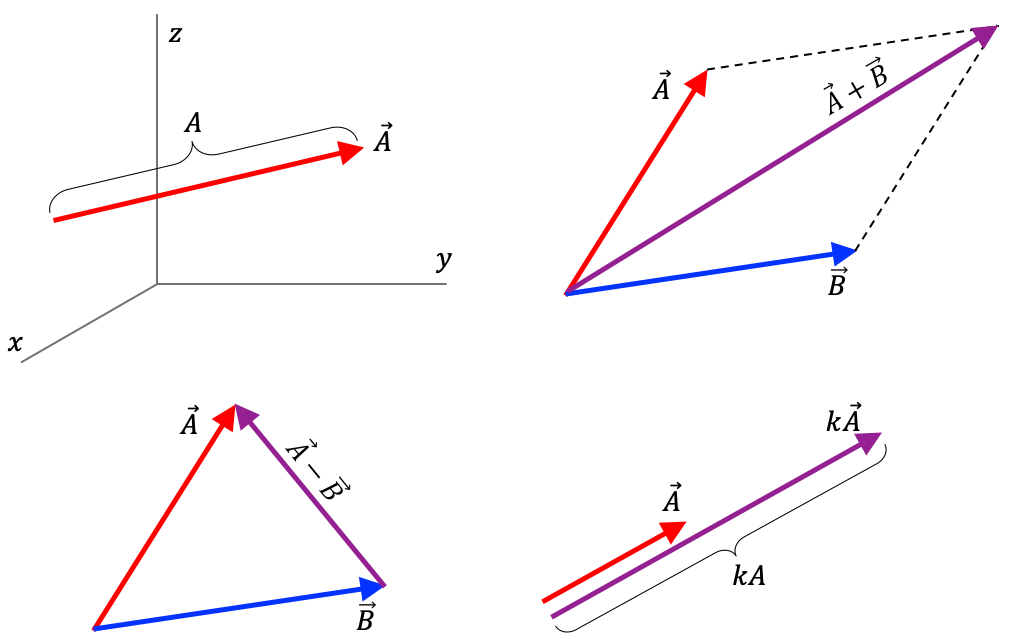
\includegraphics[width=0.8\textwidth]{./figures/square_vectores_definicion.png}
\caption{Definición geométrica de vector espacial y de sus operaciones
básicas (suma, resta y multiplicación por un escalar). Aunque la resta
de \(\vec A-\vec B\) es un caso particular de la suma, es importante
aquí familiarizarse con la dirección que tiene este vector (va de la
cabeza del sustraendo \(\vec B\) a la del minuendo
\(\vec A\).)\label{fig:vectores}}
\end{figure}

\begin{itemize}
\item
  \textbf{Vectores geométricos (euclidianos)}. Los vectores geométricos
  o en breve vectores, son \emph{segmentos orientados} en el espacio de
  tres dimensiones (ver \autoref{fig:vectores}) que tienen las
  siguientes propiedades:

  \begin{itemize}
  \item
    Se denotarán en este libro como \(\vec A\) o \(\hat e\) (este último
    es un vector unitario) en lugar de usar la notación más común con
    letras en negrilla.
  \item
    Todo vector tiene: 1) magnitud, \(A\), igual a la longitud
    (euclidiana) del segmento correspondiente y 2) una dirección en el
    espacio.
  \item
    Los vectores forman con los números reales, un espacio vectorial con
    operaciones definidas, geométricamente, como se muestra en la
    \autoref{fig:vectores}.
  \item
    El elemento neutro de la operación suma entre vectores, es el vector
    nulo, que representaremos como \(\vec 0\).
  \item
    Todo vector, por definición, se puede escribir como una combinación
    lineal de tres vectores de una base ortonormal:
    \(\hat{e}_0,\hat{e}_1,\hat{e}_2\). Los coeficientes de la
    combinación se conocen como componentes del vector:

    \begin{equation}
    \label{eq:vectores_en_base}
    \vec A=A_0\hat{e}_0+A_1\hat{e}_1+A_2\hat{e}_2.
    \end{equation}
  \item
    El espacio de vectores es \emph{isomorfico} a el espacio vectorial
    de tripletas. Por la misma razón nos referiremos al vector, o bien
    como la entidad abstracta \(\vec A\), como su representación en
    términos de los vectores unitarios de una base ortonormal (ver ítem
    anterior) o aún mejor, en términos de la tripleta:

    \[
    \vec A:(A_0,A_1,A_2)
    \]

    En este caso usaremos el símbolo ``:'' en lugar de ``='' para dar
    entender que el vector \emph{no es} una tripleta sino una entidad
    geométrica más abstracta.

    El isomorfismo implica también, que las componentes de los vectores
    en las operaciones geométricas definidas en la
    \autoref{fig:vectores}, cumplen la Ecs. (\ref{eq:suma_tuplas}) y
    (\ref{eq:k_tupla}).
  \item
    Además de la suma y la multiplicación por un escalar, que
    caracterizan el espacio vectorial, se definen dos productos
    adicionales:

    \begin{itemize}
    \item
      \textbf{Producto escalar} o \textbf{producto punto},
      \(\vec A\cdot\vec B\). El producto escalar se define, a partir los
      vectores unitarios de la base, como:

      \[\hat{e}_i\cdot \hat{e}_j=\delta_{ij},\]

      donde \(\delta_{ij}\) es el ``delta de kroenecker'':

      \begin{equation}
        \label{eq:delta_kroenecker}
        \delta_{ij}=\left\{
        \begin{array}{ccc}
        1 & & i=j\\
        0 & & i\neq j\\
        \end{array}
        \right.
        \end{equation}

      Con esta esta definición y usando la representación de los
      vectores dada por la Ec. (\ref{eq:vectores_en_base}) puede
      probarse que:

      \[
        \vec A\cdot\vec B=A_0B_0+A_1B_1+A_2B_2
        \]
    \item
      \textbf{Producto vectorial} o \textbf{producto cruz},
      \(\vec A\times\vec B\). El producto vectorial se define, a partir
      los vectores unitarios de la base, como:

      \begin{equation}
        \label{eq:base_mano_derecha}
        \hat{e}_i\times \hat{e}_j=\epsilon_{ijk}\hat{e}_k,
        \end{equation}

      donde \(\epsilon_{ijk}\) es el ``simbolo de Levi-Civita''
      (\hreffoot{https://forvo.com/word/levi-civita/\#it}{``levi
      chivita''}):

      \begin{equation}
        \label{eq:levi_civita}
        {\epsilon _{ijk}=\left\{{\begin{matrix}+1&{\mbox{si }}(i,j,k){\mbox{ es }}(0,1,2),(1,2,0){\mbox{ o }}(2,0,1)\\-1&{\mbox{si }}(i,j,k){\mbox{ es }}(2,1,0),(0,2,1){\mbox{ o }}(1,0,2)\\0&{\mbox{de otro modo }}i=j{\text{ o }}j=k{\text{ o }}k=i\end{matrix}}\right.}
        \end{equation}

      Al conjunto de vectores unitarios de una base que se definen
      cumpliendo la Ec. (\ref{eq:base_mano_derecha}) se lo llama un
      \emph{conjunto de vectores de mano derecha}.

      Con esta esta definición y usando la representación de los
      vectores dada por la Ec. (\ref{eq:vectores_en_base}) puede
      probarse que:

      \begin{equation}
        \label{eq:producto_cruz}
        \begin{array}{rcl}
        \vec A\times\vec B 
        & = & (A_1B_2-A_2B_1)\hat{e}_0+\\
        &   & -(A_0B_2-A_2B_0)\hat{e}_1+\\
        &   & (A_0B_1-A_1B_0)\hat{e}_2\\
        \end{array}
        \end{equation}

      Está última expresión es tan elaborada que con frecuencia se usa
      la regla mnemoténica:

      \begin{equation}
      \label{eq:producto_cruz_determinante}
      \vec A\times\vec B =
      \left|
      \begin{array}{ccc}
      \hat{e}_0 & \hat{e}_1 & \hat{e}_2\\
      A_0 & A_1 & A_2\\
      B_0 & B_1 & B_2\\
      \end{array}
      \right|
      \end{equation}

      Donde \(|M|\) es el determinante de la matriz \(M\).
    \end{itemize}
  \item
    Otras identidades útiles:

    \begin{itemize}
    \item
      Propiedad cíclica del \textbf{triple producto escalar}:

      \begin{equation}
       \label{eq:triple_producto_escalar}
       \vec A\cdot(\vec B\times\vec C)=
       \vec C\cdot(\vec A\times\vec B)=
       \vec B\cdot(\vec C\times\vec A)
       \end{equation}
    \item
      \textbf{Triple producto vectorial}:

      \begin{equation}
       \label{eq:triple_producto_vectorial}
       \vec A\times(\vec B\times\vec C)=(\vec A\cdot\vec C)\vec B-(\vec A\cdot\vec B)\vec C
       \end{equation}
    \end{itemize}
  \end{itemize}
\end{itemize}

\hypertarget{algoritmos-para-conjuntos-y-tuplas}{%
\subsubsection{Algoritmos para conjuntos y
tuplas}\label{algoritmos-para-conjuntos-y-tuplas}}

Todos los lenguajes modernos de programación, definen tipos especiales
para representar conjuntos y tuplas. En \texttt{Python} existen tres
tipos de objetos básicos para este propósito: \texttt{listas},
\texttt{tuplas} y diccionarios. Existen sútiles diferencias entre las
listas y las tuplas en \texttt{Python} y en general usaremos con más
frecuencia las primeras.\\
Para para los algoritmos de este libro, es importante entender las
\emph{operaciones} entre listas, que son diferentes a las operaciones en
el espacio vectorial de las tuplas matemáticas que definimos antes.

Así, por ejemplo, en el siguiente algorítmo se construye una lista con
las componentes del vector de estado de una partícula, ``sumando'' las
listas de las componentes de su vector posición y velocidad:

    \begin{code}{}{}\begin{Verbatim}[fontsize=\small,commandchars=\\\{\}]
\PY{c+c1}{\PYZsh{}Lista de componentes del vector posición}
\PY{n}{r}\PY{o}{=}\PY{p}{[}\PY{l+m+mi}{1}\PY{p}{,}\PY{l+m+mi}{0}\PY{p}{,}\PY{l+m+mi}{3}\PY{p}{]}
\PY{c+c1}{\PYZsh{}Lista de componentes del vector velocidad}
\PY{n}{v}\PY{o}{=}\PY{p}{[}\PY{l+m+mi}{0}\PY{p}{,}\PY{o}{\PYZhy{}}\PY{l+m+mi}{1}\PY{p}{,}\PY{l+m+mi}{0}\PY{p}{]}
\PY{c+c1}{\PYZsh{}Lista de componentes del vector de estado}
\PY{n}{X}\PY{o}{=}\PY{n}{r}\PY{o}{+}\PY{n}{v}
\end{Verbatim}

%%

\end{code}
\vspace{-1em}

%%hidecode


    \begin{Verbatim}[fontsize=\small,commandchars=\\\{\}]
X = [1, 0, 3, 0, -1, 0]
\end{Verbatim}

El operador \texttt{+}, entre listas y tuplas de \texttt{Python} produce
la unión de los elementos de las listas.

Usando este operador se pueden hacer algoritmos prácticos como el que se
muestra a continuación:

    \begin{code}{}{}\begin{Verbatim}[fontsize=\small,commandchars=\\\{\}]
\PY{k}{def} \PY{n+nf}{f}\PY{p}{(}\PY{n}{x}\PY{p}{)}\PY{p}{:}
    \PY{k+kn}{from} \PY{n+nn}{math} \PY{k}{import} \PY{n}{sin}
    \PY{n}{y}\PY{o}{=}\PY{n}{sin}\PY{p}{(}\PY{n}{x}\PY{p}{)}\PY{o}{/}\PY{n}{x}
    \PY{k}{return} \PY{n}{y}

\PY{n}{valores\PYZus{}de\PYZus{}x}\PY{o}{=}\PY{p}{[}\PY{l+m+mf}{1.0}\PY{p}{,}\PY{l+m+mf}{2.0}\PY{p}{,}\PY{l+m+mf}{3.0}\PY{p}{]}
\PY{n}{valores\PYZus{}de\PYZus{}f}\PY{o}{=}\PY{p}{[}\PY{p}{]}
\PY{k}{for} \PY{n}{x} \PY{o+ow}{in} \PY{n}{valores\PYZus{}de\PYZus{}x}\PY{p}{:}
    \PY{n}{valores\PYZus{}de\PYZus{}f}\PY{o}{+}\PY{o}{=}\PY{p}{[}\PY{n}{f}\PY{p}{(}\PY{n}{x}\PY{p}{)}\PY{p}{]}
\end{Verbatim}

%%

\end{code}
\vspace{-1em}

%%hidecode


    \begin{Verbatim}[fontsize=\small,commandchars=\\\{\}]
valores de f = [0.8414709848078965, 0.45464871341284085, 0.0470400026866224]
\end{Verbatim}

aquí, comenzamos con un conjunto vacío, \texttt{valores\_de\_f={[}{]}} y
después, dentro de un ciclo, usamos el operador de acumulación
\texttt{+=} para agreganr elementos al conjunto. Este es un método muy
común usado en el lenguaje para construir ``tablas de valores'', que
pueden, por ejemplo usarse para hacer gráficos de funciones.

\hypertarget{algoritmos-para-vectores}{%
\subsubsection{Algoritmos para
vectores}\label{algoritmos-para-vectores}}

Los vectores forman un ``capítulo'' en la computación separado de las
listas y las tuplas. La razón básica son sus propiedades matemáticas y
las operaciones definidas entre ellos. Bibliotecas de rutinas muy
completas existen en todos los lenguajes de programación para
representar este tipo de entidades matemáticas.

En \texttt{Python} y a lo largo de este libro usaremos los objetos y
rutinas de los paquetes \texttt{NumPy} y \texttt{SPICE} para definir y
manipular vectores.

El ejemplo abajo muestra como se calcula el ángulo entre dos vectores
\(\theta_{AB}\), a partir de la interpretación geométrica del producto
punto \(\vec{A}\cdot\vec{B}=AB\cos\theta_{AB}\) (ver problemas al final
del capítulo):

    \begin{code}{}{}\begin{Verbatim}[fontsize=\small,commandchars=\\\{\}]
\PY{c+c1}{\PYZsh{}Definimos los vectores}
\PY{k+kn}{from} \PY{n+nn}{numpy} \PY{k}{import} \PY{n}{array}
\PY{n}{A}\PY{o}{=}\PY{n}{array}\PY{p}{(}\PY{p}{[}\PY{l+m+mf}{1.0}\PY{p}{,}\PY{l+m+mf}{0.0}\PY{p}{,}\PY{l+m+mf}{2.0}\PY{p}{]}\PY{p}{)}
\PY{n}{B}\PY{o}{=}\PY{n}{array}\PY{p}{(}\PY{p}{[}\PY{l+m+mf}{0.0}\PY{p}{,}\PY{l+m+mf}{1.0}\PY{p}{,}\PY{l+m+mf}{3.0}\PY{p}{]}\PY{p}{)}

\PY{c+c1}{\PYZsh{}Calculamos el producto escalar y vectorial}
\PY{k+kn}{from} \PY{n+nn}{numpy} \PY{k}{import} \PY{n}{dot}
\PY{n}{ApuntoB}\PY{o}{=}\PY{n}{dot}\PY{p}{(}\PY{n}{A}\PY{p}{,}\PY{n}{B}\PY{p}{)}

\PY{c+c1}{\PYZsh{}El ángulo entre los vectores}
\PY{k+kn}{from} \PY{n+nn}{numpy} \PY{k}{import} \PY{n}{arccos}
\PY{k+kn}{from} \PY{n+nn}{numpy}\PY{n+nn}{.}\PY{n+nn}{linalg} \PY{k}{import} \PY{n}{norm}
\PY{n}{anguloAB}\PY{o}{=}\PY{n}{arccos}\PY{p}{(}\PY{n}{ApuntoB}\PY{o}{/}\PY{p}{(}\PY{n}{norm}\PY{p}{(}\PY{n}{A}\PY{p}{)}\PY{o}{*}\PY{n}{norm}\PY{p}{(}\PY{n}{B}\PY{p}{)}\PY{p}{)}\PY{p}{)}
\end{Verbatim}

%%

\end{code}
\vspace{-1em}

%%hidecode


    \begin{Verbatim}[fontsize=\small,commandchars=\\\{\}]
AnguloAB = 31.948059431330062 grados
\end{Verbatim}
\begin{box_note}{Nota}

\textbf{Radianes y grados en los algoritmos.} Es importante entender que
las funciones trigonométricas inversas como \texttt{arccos}, devuelven,
en todos los lenguajes de programación, valores de los ángulos en
radianes. En el caso anterior, por ejemplo, el valor de la variable
\texttt{anguloAB} al final del algoritmo en realidad era
\texttt{0.5575988266995369}. Sin embargo, decidimos mostrar su valor en
grados después de multiplicar \texttt{anguloAB} por el factor de
conversión \(\pi/180\) (esta operación no se muestra en el código.) Así
lo seguiremos haciendo en el resto del libro. El lector que use los
algoritmos no debe olvidar multiplicar por el factor de conversión para
reconstruir los resultados mostrados aquí.

\end{box_note}
Un procedimiento similar, esta vez usando vectores y rutinas de
\texttt{SPICE} (internamente \texttt{SPICE} usa vectores o arreglos de
\texttt{NumPy}), puede usarse para calcular el triple producto
vectorial:

    \begin{code}{}{}\begin{Verbatim}[fontsize=\small,commandchars=\\\{\}]
\PY{k+kn}{from} \PY{n+nn}{numpy} \PY{k}{import} \PY{n}{array}
\PY{k+kn}{from} \PY{n+nn}{spiceypy} \PY{k}{import} \PY{n}{vdot}\PY{p}{,}\PY{n}{vcrss}

\PY{n}{A}\PY{o}{=}\PY{n}{array}\PY{p}{(}\PY{p}{[}\PY{l+m+mf}{2.0}\PY{p}{,}\PY{l+m+mf}{2.0}\PY{p}{,}\PY{l+m+mf}{1.0}\PY{p}{]}\PY{p}{)}
\PY{n}{B}\PY{o}{=}\PY{n}{array}\PY{p}{(}\PY{p}{[}\PY{l+m+mf}{0.0}\PY{p}{,}\PY{o}{\PYZhy{}}\PY{l+m+mf}{1.0}\PY{p}{,}\PY{l+m+mf}{0.0}\PY{p}{]}\PY{p}{)}
\PY{n}{C}\PY{o}{=}\PY{n}{array}\PY{p}{(}\PY{p}{[}\PY{l+m+mf}{0.0}\PY{p}{,}\PY{l+m+mf}{0.0}\PY{p}{,}\PY{l+m+mf}{2.0}\PY{p}{]}\PY{p}{)}

\PY{n}{AxBxC}\PY{o}{=}\PY{n}{vdot}\PY{p}{(}\PY{n}{A}\PY{p}{,}\PY{n}{B}\PY{p}{)}\PY{o}{*}\PY{n}{C}\PY{o}{\PYZhy{}}\PY{n}{vdot}\PY{p}{(}\PY{n}{A}\PY{p}{,}\PY{n}{C}\PY{p}{)}\PY{o}{*}\PY{n}{B}
\end{Verbatim}

%%

\end{code}
\vspace{-1em}

%%hidecode


    \begin{Verbatim}[fontsize=\small,commandchars=\\\{\}]
A x (B x C) = [-0.  2. -4.]
\end{Verbatim}

También podemos usarlas para verificar la propiedad cíclica del triple
producto escalar:

    \begin{code}{}{}\begin{Verbatim}[fontsize=\small,commandchars=\\\{\}]
\PY{k+kn}{from} \PY{n+nn}{numpy} \PY{k}{import} \PY{n}{array}
\PY{k+kn}{from} \PY{n+nn}{spiceypy} \PY{k}{import} \PY{n}{vnorm}\PY{p}{,}\PY{n}{vdot}\PY{p}{,}\PY{n}{vcrss}
\PY{n}{A}\PY{o}{=}\PY{n}{array}\PY{p}{(}\PY{p}{[}\PY{l+m+mf}{2.0}\PY{p}{,}\PY{l+m+mf}{2.0}\PY{p}{,}\PY{l+m+mf}{1.0}\PY{p}{]}\PY{p}{)}
\PY{n}{B}\PY{o}{=}\PY{n}{array}\PY{p}{(}\PY{p}{[}\PY{l+m+mf}{0.0}\PY{p}{,}\PY{o}{\PYZhy{}}\PY{l+m+mf}{1.0}\PY{p}{,}\PY{l+m+mf}{0.0}\PY{p}{]}\PY{p}{)}
\PY{n}{C}\PY{o}{=}\PY{n}{array}\PY{p}{(}\PY{p}{[}\PY{l+m+mf}{0.0}\PY{p}{,}\PY{l+m+mf}{0.0}\PY{p}{,}\PY{l+m+mf}{2.0}\PY{p}{]}\PY{p}{)}

\PY{n}{ABC}\PY{o}{=}\PY{n}{vdot}\PY{p}{(}\PY{n}{A}\PY{p}{,}\PY{n}{vcrss}\PY{p}{(}\PY{n}{B}\PY{p}{,}\PY{n}{C}\PY{p}{)}\PY{p}{)}
\PY{n}{CAB}\PY{o}{=}\PY{n}{vdot}\PY{p}{(}\PY{n}{C}\PY{p}{,}\PY{n}{vcrss}\PY{p}{(}\PY{n}{A}\PY{p}{,}\PY{n}{B}\PY{p}{)}\PY{p}{)}
\PY{n}{BCA}\PY{o}{=}\PY{n}{vdot}\PY{p}{(}\PY{n}{B}\PY{p}{,}\PY{n}{vcrss}\PY{p}{(}\PY{n}{C}\PY{p}{,}\PY{n}{A}\PY{p}{)}\PY{p}{)}
\end{Verbatim}

%%

\end{code}
\vspace{-1em}

%%hidecode


    \begin{Verbatim}[fontsize=\small,commandchars=\\\{\}]
A.(BxC) = -4.0
C.(AxB) = -4.0
B.(CxA) = -4.0
\end{Verbatim}

Con lo que se verifica la identidad (al menos para los vectores
escogidos.)

\hypertarget{sistemas_coordenadas}{%
\subsection{Sistemas de coordenadas}\label{sistemas_coordenadas}}

\begin{figure}[t]
\centering
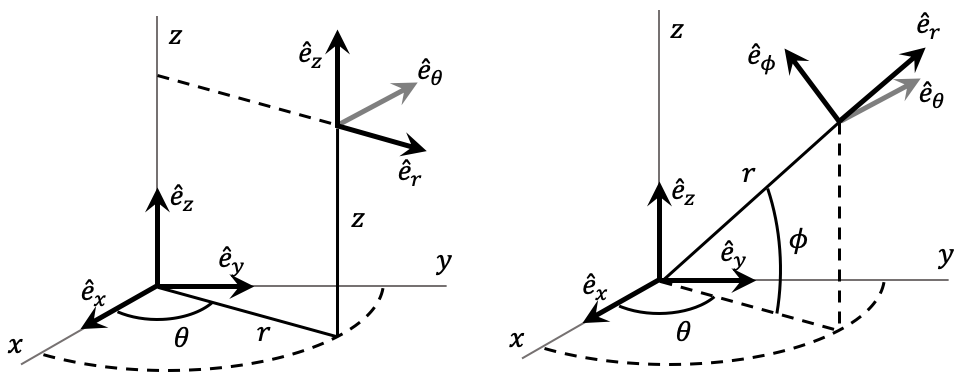
\includegraphics[width=1\textwidth]{./figures/horizontal_sistemas_coordenadas.png}
\caption{Definción de los sistemas de coordenadas usadas en este
texto\label{fig:coordenadas}}
\end{figure}

A lo largo de este libro, usaremos los tres sistemas de coordenadas
ortogonales \emph{clásicos} (cartesianas, cilíndricas y esféricas, ver
\autoref{fig:coordenadas}) con algunas convenciones más propias de la
astronomía y la mecánica celeste que del cálculo.

A continuación, y en especial para clarificar nuestra notación,
enumeramos detalladamente las propiedades de cada sistema.

\begin{itemize}
\item
  \textbf{Sistema de coordenadas cartesiano}.

  \begin{itemize}
  \item
    Coordenadas: \(x\in(-\infty,+\infty)\), \(y\in(-\infty,+\infty)\),
    \(z\in(-\infty,+\infty)\).
  \item
    Vectores unitarios: \(\hat{e}_x\), \(\hat{e}_y\), \(\hat{e}_z\).
  \item
    Comentarios:

    \begin{itemize}
    \tightlist
    \item
      En todos los casos la orientación de los ejes obedecerá la
      \emph{regla de la mano derecha}, es decir, los sistemas
      cartesianos usados en el texto y cuyos ejes están definidos por el
      conjunto de vectores unitarios (\(\hat{e}_x\), \(\hat{e}_y\),
      \(\hat{e}_z\)) forman un \emph{conjunto de mano derecha} (ver Ec.
      \ref{eq:base_mano_derecha}), a saber, en forma explícita:
    \end{itemize}
  \end{itemize}

  \begin{equation}
  \label{eq:conjunto_mano_derecha}
  \begin{array}{ccl}
  \hat{e}_x\times\hat{e}_y & = & \hat{e}_z\\
  \hat{e}_y\times\hat{e}_z & = & \hat{e}_x\\
  \hat{e}_z\times\hat{e}_x & = & \hat{e}_y
  \end{array}
  \end{equation}
\end{itemize}

\begin{itemize}
\item
  \textbf{Sistema de coordenadas cilíndrico} (ver
  \autoref{fig:coordenadas}).

  \begin{itemize}
  \item
    Coordenadas: \(r\in[0,+\infty)\), \(\theta\in[0,2\pi)\),
    \(z\in(-\infty,+\infty)\).
  \item
    Conversión al sistema de coordenadas cartesianas:

    \begin{equation}
      \label{eq:cilindricas_a_cartesianas}
      \begin{array}{ccl}
      x & = & r\cos\theta\\
      y & = & r\sin\theta\\
      \end{array}
      \end{equation}
  \item
    Vectores unitarios expresados en el sistema de coordenadas
    cartesianas:

    \begin{equation}
      \label{eq:unitarios_cilindricas}
      \begin{array}{ccl}
      \hat{e}_r & = & \cos\theta\;\hat{e}_x + \sin\theta\;\hat{e}_y\\
      \hat{e}_\theta & = & -\sin\theta\;\hat{e}_x + \cos\theta\;\hat{e}_y\\
      \hat{e}_z & = & \hat{e}_z
      \end{array}
      \end{equation}
  \item
    Comentarios:

    \begin{itemize}
    \item
      El conjunto de vectores unitarios (\(\hat{e}_r\),
      \(\hat{e}_\theta\), \(\hat{e}_z\)) forman un conjunto de mano
      derecha tal y como se definió en las Ecs.
      (\ref{eq:conjunto_mano_derecha}).
    \item
      Nótese que, a diferencia de la notación usada generalmente en los
      textos de cálculo, la coordenada cilíndrica \(r\) usa la misma
      letra que la coordenada esférica \(r\) y la magnitud del vector
      posición (ver siguiente sección). La distinción entre las tres,
      dependerá del contexto.
    \item
      Usaremos la letra griega \(\theta\) para denotar el ángulo
      \emph{acimutal}, a diferencia de la notación convencional que usa
      esta letra para la coordenada esférica polar (ángulo del vector
      posición respecto al eje z.)
    \end{itemize}
  \end{itemize}
\end{itemize}

\begin{itemize}
\item
  \textbf{Sistema de coordenadas esférico} (ver
  \autoref{fig:coordenadas}).

  \begin{itemize}
  \item
    Coordenadas: \(r\in[0,+\infty)\), \(\theta\in[0,2\pi)\),
    \(\phi\in[-\pi/2,+\pi/2]\).
  \item
    Conversión al sistema de coordenadas cartesianas:

    \begin{equation}
      \label{eq:esfericas_a_cartesianas}
      \begin{array}{ccl}
      x & = & r\cos\phi\cos\theta\\
      y & = & r\cos\phi\sin\theta\\
      z & = & r\sin\phi\\
      \end{array}
      \end{equation}
  \item
    Vectores unitarios expresados en el sistema de coordenadas
    cartesianas:

    \begin{equation}
      \label{eq:unitarios_esfericas}
      \begin{array}{ccl}
      \hat{e}_r & = & \cos\phi\cos\theta\;\hat{e}_x + \cos\phi\sin\theta\;\hat{e}_y + \sin\phi\;\hat{e}_z\\
      \hat{e}_\theta & = & -\sin\theta\;\hat{e}_x + \cos\theta\;\hat{e}_y\\
      \hat{e}_\phi & = & \cos\phi\cos\theta\;\hat{e}_x + \sin\phi\sin\theta\;\hat{e}_y - \sin\phi\;\hat{e}_z\\
      \end{array}
      \end{equation}
  \item
    Comentarios:

    \begin{itemize}
    \item
      El conjunto de vectores unitarios (\(\hat{e}_r\),
      \(\hat{e}_\theta\), \(\hat{e}_\phi\)) forman un conjunto de mano
      derecha tal y como se definió en las Ecs.
      (\ref{eq:conjunto_mano_derecha}).
    \item
      Nótese que, a diferencia de la notación usada generalmente en los
      textos de cálculo, la coordenada esférica \(\phi\) se medirá
      respecto al plano \(x-y\) (como una \emph{latitud}) en lugar de
      hacerlo respecto al eje \(z\) (como una \emph{colatitud}).
    \end{itemize}
  \end{itemize}
\end{itemize}

Una interesante página interactiva que permite visualizar mejor la
definición de los sistemas de coordenadas y la orientación de los
vectores coordenadas puede encontrarse en los siguientes enlaces, tanto
para el \hreffoot{http://dynref.engr.illinois.edu/rvy.html}{sistema de
coordenadas cilíndrica} como para el
\hreffoot{http://dynref.engr.illinois.edu/rvy.html}{sistema de coordenadas
esféricas}.



\hypertarget{funciones}{%
\subsection{Funciones}\label{funciones}}

Una función es, en términos informales, una regla de correspondencia que
asocia los elementos de un conjunto de partida o \emph{dominio} (p.e. el
conjunto de los números reales \({\rm I\!R}\), el conjunto de puntos en
un plano \({\rm I\!R}^2\) o de eventos en el espacio tiempo
\({\rm I\!R}^4\)) con los de otro conjunto, llamado rango, de modo a que
cada elemento del dominio le corresponde \textbf{uno y solo un elemento
del rango}.

Entre los distintos tipos de funciones que reconoce el análisis
matemático, en este libro nos concentraremos en:

\begin{itemize}
\tightlist
\item
  \textbf{Funciones de variable real}: Dominio y rango \({\rm I\!R}\).
  Ejemplo: \(f(t)=t^2\).
\item
  \textbf{Funciones de muchas variables} o \textbf{Campos escalares}:
  Dominio \({\rm I\!R}^n\), rango \({\rm I\!R}\). Ejemplos:
  \(f(x,y)=x^2+y^2\), \(H(\{q_i\}_N)=\sum_i q_i^2\) (para la notación
  del conjunto \(\{q_i\}\) ver la
  \autoref{conjuntos_tuplas_vectores}).
\item
  \textbf{Funciones vectoriales}: Dominio \({\rm I\!R}\), rango
  \({\rm I\!R}^n\). Ejemplo: \(\vec a(t)=kr^{-n} \hat{e}_r\).
\item
  \textbf{Funciones vectoriales de muchas variables} o \textbf{Campos
  vectoriales}: Dominio \({\rm I\!R}^n\), rango \({\rm I\!R}^3\).
  Ejemplo: \(\vec{F}(r,\theta,z):-k(r\cos\theta,r\sin\theta,z)\).
\end{itemize}
\begin{box_note}{Nota}

\textbf{\(t\) como variable genérica de las funciones.} En todos los
textos de matemáticas (incluso en los de física) se acostumbra usar
\(x\) como el nombre preferido para representar, de forma genérica, la
variable independiente de las funciones. En lo sucesivo cambiaremos esta
convención al llamar \(t\) a la variable independiente genérica. La
razón no puede ser más sencilla: en la mecánica \(t\) es el nombre que
damos a la variable independiente por excelencia, el tiempo, de modo que
muchas de las fórmulas que desarrollaremos en este capítulo, se
trasladaran simbólicamente casi sin modificación a la mecánica.

Es obvio que la elección de la letra con la que representamos la
variable independiente, no modifica en nada las definiciones y teoremas
que veremos en esta sección, de modo que esperamos esta elección no
moleste a los más conservadores ni confunda a quienes han estudiado
ampliamente estos temas en otros textos.

\end{box_note}
\hypertarget{algoritmos-para-funciones}{%
\subsubsection{Algoritmos para
funciones}\label{algoritmos-para-funciones}}

Hay dos maneras de definir una función en \texttt{Python}: 1) como una
rutina o 2) como una función \texttt{lambda}.

Como una rutina, una función en \texttt{Python} puede recibir como
``argumentos'' de entrada no solo las variables de la función sino
también argumentos opcionales.

La siguiente función, por ejemplo, permite calcular el valor de la
energía potencial de un sistema físico usando la función de varias
variables \(U(\vec r)=kr^{n}\) (siendo \(\vec r:x,y,z\) el vector
posición y \(r\) su magnitud.)

    \begin{code}{Algoritmo}{code:rutina_potencial}\begin{Verbatim}[fontsize=\small,commandchars=\\\{\}]
\PY{k}{def} \PY{n+nf}{U}\PY{p}{(}\PY{n}{x}\PY{p}{,}\PY{n}{y}\PY{p}{,}\PY{n}{z}\PY{p}{,}\PY{n}{k}\PY{o}{=}\PY{l+m+mi}{1}\PY{p}{,}\PY{n}{n}\PY{o}{=}\PY{o}{\PYZhy{}}\PY{l+m+mi}{1}\PY{p}{)}\PY{p}{:}
    \PY{n}{r}\PY{o}{=}\PY{p}{(}\PY{n}{x}\PY{o}{*}\PY{o}{*}\PY{l+m+mi}{2}\PY{o}{+}\PY{n}{y}\PY{o}{*}\PY{o}{*}\PY{l+m+mi}{2}\PY{o}{+}\PY{n}{z}\PY{o}{*}\PY{o}{*}\PY{l+m+mi}{2}\PY{p}{)}\PY{o}{*}\PY{o}{*}\PY{l+m+mf}{0.5}
    \PY{k}{return} \PY{n}{k}\PY{o}{*}\PY{n}{r}\PY{o}{*}\PY{o}{*}\PY{n}{n}
\end{Verbatim}

%%

\end{code}
\vspace{-1em}

%%hidecode


    \begin{Verbatim}[fontsize=\small,commandchars=\\\{\}]
U(1.0,2.0,0.0) con k = 1 y n = -1 (valores por defecto) = 0.4472135954999579
U(1.0,2.0,0.0) con k = 6.67e-11 y n = -2 = 1.334e-11
\end{Verbatim}
\begin{box_note}{Nota}

\textbf{Argumentos obligatorios y argumentos opcionales.} Toda rutina en
\texttt{Python} puede tener unos argumentos obligatorios (que llamaremos
variables) o unos opcionales.

Las variables son en estricto sentido una \texttt{tupla} de valores, por
ejemplo \texttt{x,y,z} en la función \(U\) en el Alg.
(\ref{code:rutina_potencial}).

Los argumentos opcionales son, por otro lado, un \texttt{diccionario} de
valores, que no es otra cosa que una lista de valores identificados con
un nombre (también llamdo clave o \texttt{key}). En la función \(U\) en
el Alg. (\ref{code:rutina}) los argumentos opcionales son
\texttt{k=1,n=-1}.

En \texttt{Python} las variables y las opciones de una rutina pueden
representarse usando los objetos especiales \texttt{*variables} y
\texttt{**opciones}. El uso de estos objetos especiales no es muy común,
pero en ciertas situaciones puede ser bastante útil.

Una forma alternativa de la rutina para \(U\) en el Alg.
(\ref{code:rutina}) es:

\begin{Shaded}
\begin{Highlighting}[]
\KeywordTok{def}\NormalTok{ U(}\OperatorTok{*}\NormalTok{variables,}\OperatorTok{**}\NormalTok{opciones):}
\NormalTok{  x,y,z}\OperatorTok{=*}\NormalTok{variables}
\NormalTok{  r}\OperatorTok{=}\NormalTok{(x}\OperatorTok{**}\DecValTok{2}\OperatorTok{+}\NormalTok{y}\OperatorTok{**}\DecValTok{2}\OperatorTok{+}\NormalTok{z}\OperatorTok{**}\DecValTok{2}\NormalTok{)}\OperatorTok{**}\FloatTok{0.5}
  \ControlFlowTok{return}\NormalTok{ opciones[}\StringTok{"k"}\NormalTok{]}\OperatorTok{*}\NormalTok{r}\OperatorTok{**}\NormalTok{n}
\end{Highlighting}
\end{Shaded}

que se puede invocar usando:

\begin{Shaded}
\begin{Highlighting}[]
\NormalTok{var}\OperatorTok{=}\FloatTok{1.0}\NormalTok{,}\FloatTok{2.0}
\NormalTok{opc}\OperatorTok{=}\BuiltInTok{dict}\NormalTok{(k}\OperatorTok{=}\DecValTok{1}\NormalTok{,n}\OperatorTok{=-}\DecValTok{2}\NormalTok{)}
\NormalTok{U(}\OperatorTok{*}\NormalTok{var,}\OperatorTok{**}\NormalTok{opc)}
\end{Highlighting}
\end{Shaded}

No parece muy práctico, pero como veremos puede ser muy útil en ciertas
situaciones especiales.

\end{box_note}
Las funciones \texttt{lambda} se usan para representar funciones muy
abreviadas y no tienen argumentos distintos de las variables de las que
dependen.

Así, por ejemplo, el siguiente algoritmo define una función
\texttt{lambda}, \texttt{U\_x}, basada en la función \(U\) del Alg.
(\ref{code:rutina}), que depende solo de la variable \(x\) cuando y
asumes constante los valores de \(y\) y \(z\) (\texttt{U\_x} será util
para calcular más abajo la derivadas parcial de \(U\) respecto a \(x\)):

    \begin{code}{Algoritmo}{code:funcion_lambda}\begin{Verbatim}[fontsize=\small,commandchars=\\\{\}]
\PY{n}{y}\PY{o}{=}\PY{l+m+mf}{1.0}
\PY{n}{z}\PY{o}{=}\PY{l+m+mf}{1.0}
\PY{n}{k}\PY{o}{=}\PY{l+m+mi}{1}
\PY{n}{n}\PY{o}{=}\PY{o}{\PYZhy{}}\PY{l+m+mi}{2}
\PY{n}{U\PYZus{}x}\PY{o}{=}\PY{k}{lambda} \PY{n}{x}\PY{p}{:}\PY{n}{U}\PY{p}{(}\PY{n}{x}\PY{p}{,}\PY{n}{y}\PY{p}{,}\PY{n}{z}\PY{p}{,}\PY{n}{k}\PY{p}{,}\PY{n}{n}\PY{p}{)}
\end{Verbatim}

%%

\end{code}
\vspace{-1em}

%%hidecode


    \begin{Verbatim}[fontsize=\small,commandchars=\\\{\}]
Ux(0.0) = 0.49999999999999994
\end{Verbatim}

\hypertarget{derivadas}{%
\subsection{Derivadas}\label{derivadas}}

La derivada de una función de variable real es en sí misma una función
definida por el límite:

\begin{equation}
\label{eq:derivada_definicion}
\frac{\mathrm{d}f}{\mathrm{d}t}\equiv\lim_{\Delta t\rightarrow 0}\frac{f(t)-f(t+\Delta t)}{\Delta t}
\end{equation}

Si el límite no existe decimos que la función no es derivable en \(t\).
\begin{box_note}{Nota}

\textbf{Notación de la derivada.} A lo largo de la historia la manera
como se ha representado la función derivada ha cambiado. Existen al
menos tres notaciones comunes:

\begin{itemize}
\tightlist
\item
  La \textbf{notación de Leibniz}, \(\mathrm{d}f/\mathrm{dt}\),
  \(\mathrm{d}^2f/\mathrm{d}t^2\). En esta notación la derivada se
  representa como si fuera la razón entre dos cantidades, pero no es así
  ¡mucho cuidado! Usaremos la notación de Leibniz especialmente para
  representar la derivada de funciones que se escriben de forma
  explícita, así por ejemplo:
\end{itemize}

\[ 
  \frac{\mathrm{d}}{\mathrm{d}t}\left(\frac{1}{2} t^2\right)
  \]

\begin{itemize}
\item
  La \textbf{notación de Newton}, \(\dot f\), \(\ddot f\). Esta será la
  forma que usaremos para denotar a lo largo del libro las derivadas
  respecto del tiempo (o el tiempo propio en relatividad).
\item
  La \textbf{notación de Lagrange}, \(f'\), \(f''\), \(f^{(n)}\).
\item
  La \textbf{notación de Euler}, \(\mathrm{D}f\), \(\mathrm{D}^2f\),
  \(\mathrm{D}^{n} f\), que no usaremos aquí pero es la notación menos
  común, pero puede aparecer en el contexto de la mecánica de fluídos.
\end{itemize}

\end{box_note}
La definición de derivada de las funciones de variable real como un
límite, se extiende por analogía a campos escalares, funciones
vectoriales o campos vectoriales. Para las funciones que dependen de
varias variables, sin embargo, se usa una notación y un nombre
diferente: \textbf{derivada parcial}. La derivada parcial de un campo
escalar se define como:

\[
\frac{\partial f}{\partial q_k}=
\lim_{\Delta q_k\rightarrow 0}\frac{
f(q_1,q_2,\ldots,q_k+\Delta q_k,\ldots,q_N)-
f(q_1,q_2,\ldots,q_k,\ldots,q_N)
}{\Delta q_k}
\]

La derivada parcial se calcula de la misma manera que la derivada de una
variable, con la salvedad de que al hacerlo se asume que todas las demás
variables de la función son constantes.

En muchas partes en este libro, y por economía usaremos la notación de
Euler para las derivadas parciales, a saber:

\[
\partial_x f\equiv\frac{\partial f}{\partial x}
\]

En esta notación una derivada parcial múltiple se escribirá como:

\[
\partial_{xyz}f(x,y,z)\equiv\frac{\partial^3 f}{\partial x\partial y\partial z}
\]

A pesar de que la derivada parcial tiene una definición \emph{numérica}
análoga a la de la derivada total, existe una sútil diferencia entre
ambas.

Imagine que tenemos una \textbf{variable independiente} \(t\) y
definimos, a partir de ella, una nueva variable \(u\) que es función de
\(t\) (variable dependiente).

¿Cómo podemos calcular la derivada de una función de la nueva variable
\(f(u)\) respecto de la variable independiente \(t\)?
\begin{box_theorem}{Proposición}{box:teo:regla.cadena}

\textbf{Regla de la Cadena.} Dada una función compuesta \(f(u(t))\), la
derivada de \(f\) respecto a \(t\) es:

\[
\frac{\mathrm{d}f}{\mathrm{d}t}=\frac{\mathrm{d}f}{\mathrm{d}u}\frac{\mathrm{d}u}{\mathrm{d}t}
\]

\end{box_theorem}
Decimos que la función \(f\) depende \emph{implícitamente} de la
variable independiente \(t\). En este sentido la regla de la cadena es
una regla de \emph{derivación implícita}.

Usando la notación de Newton la expresión anterior se escribirá de forma
abreviada:

\[
\dot{f}(t)=\dot u\frac{\mathrm{d}f}{\mathrm{d}u}
\]

¿Qué pasa en el caso en el que \(f\) depende de varias variables
dependientes, por ejemplo
\(f(q_1(t),q_2(t),\ldots, q_N(t))\equiv f(\{q_i(t)\}_N)\)?

En este caso la regla de la cadena se puede generalizar como:

\[
\frac{\mathrm{d}f}{\mathrm{d}t}=
\frac{\partial f}{\partial q_1}\frac{\mathrm{d}q_1}{\mathrm{d}t}+
\frac{\partial f}{\partial q_2}\frac{\mathrm{d}q_2}{\mathrm{d}t}+
\ldots
\frac{\partial f}{\partial q_N}\frac{\mathrm{d}q_N}{\mathrm{d}t}=
\sum_i \frac{\partial f}{\partial q_i}\frac{\mathrm{d}q_i}{\mathrm{d}t}=
\sum_i \dot{q}_i\partial_{q_i} f 
\]

Ahora bien: ¿existirá, en este caso, la derivada parcial de \(f\)
respecto de \(t\)?

La respuesta a esta pregunta, ilustra, justamente, la diferencia sutil
entre la derivada ordinaria o \emph{derivada total}
\(\mathrm{d}/\mathrm{dt}\) y la derivada parcial
\(\partial/\partial t\).

Hay dos situaciones posibles:

\begin{itemize}
\item
  Si la función \(f\) \emph{no depende} explícitamente de \(t\), es
  decir si la variable \(t\) no aparece en la fórmula de \(f\), entonces
  \(\partial f/\partial t=0\). Este resultado es \emph{independiente} de
  que \(f\) dependa implícitamente de \(t\) a través de otras variables
  dependientes.

  \textbf{Ejemplo}: si \(f(q,t)=q^2\), entonces:
  \(\partial f/\partial t=0\) aunque, por regla de la cadena,
  \(\mathrm{d}f/\mathrm{d}t=2 q\dot q\).
\item
  Si la fórmula de la función \(f\) contiene la variable \(t\), entonces
  su derivada parcial puede ser distinta de cero (dependiendo de la
  forma funcional de \(f\)).

  \textbf{Ejemplo}: Si \(f(q,t)=q^2+\sin t\), entonces:
  \(\partial f/\partial t=\cos t\) y
  \(\mathrm{d}f/\mathrm{d}t=2 q\dot q+\cos t\).
\end{itemize}

En este sentido la derivada parcial es como un ``operador semántico'',
es decir un operador sobre las ``letras'' que aparecen en la fórmula de
la función.

Teniendo en cuenta esta propiedad, la forma más general de la regla de
la cadena, para una función de varias variables (campo escalar o
vectorial) será:

\begin{equation}
\label{eq:regla_cadena_general}
\frac{\mathrm{d}}{\mathrm{d}t}f(\{q_i\},t)=
\sum_i \dot{q}_i\partial_{q_i} f + \frac{\partial f}{\partial t}
\end{equation}

\hypertarget{funciones_homogeneas}{%
\subsection{Funciones homogéneas}\label{funciones_homogeneas}}

Existe un interesante conjunto de funciones para las cuáles hay una
relación no trivial entre su derivada y el valor de la función misma. Se
conocen como \textbf{funciones homogéneas}:
\begin{box_definition}{Definición}{box:def:funciones.homogeneas}

\textbf{Funciones homogéneas.} Una función general \(f(\{q_i\})\) se
llama homogénea si frente a una operación de escalado de sus variables
(multiplicación por un escalar), la función \emph{escala} también. En
términos matemáticos:

\[
  f(\{\lambda q_i\})=\lambda^k f(\{q_i\})
  \]

donde \(\lambda\) es un número real y \(k\) se conoce como el
\textbf{orden} de la función.

\end{box_definition}
Las funciones homogéneas son, generalmente polinomios y funciones
racionales. Así por ejemplo \(f(x,y)=x^2/a^2+y^2/b^2\), con \(a\) y
\(b\) constantes, y que representa la ecuación algebraica de una elipse,
es una función homogénea de grado \(k=2\). De otro lado
\(f(x)=x^3y^2+y^5\) es homogénea de grado \(k=5\).

Las funciones homogéneas más interesantes para nosotros en este libro
son del tipo \(f(\vec r)=k r^n\) que son homogéneas de grado \(k=n\)
(ver problemas al final del capítulo.)

Como mencionamos desde el principio, las derivadas de las funciones
homogéneas tienen una propiedad muy importante:
\begin{box_theorem}{Proposición}{box:teo:funciones.homogeneas.euler}

\textbf{Teorema de funciones homogeneas de de Euler.} Si una función
\(f(\{q_i\}_N)\) es homogénea de grado \(k\), entonces:

\[
  \sum_i q_i \frac{\partial f}{\partial q_i} = k f
  \]

\end{box_theorem}
Para funciones homogéneas definidas en el espacio de tres dimensiones,
el teorema de Euler se puede escribir como:

\[
\vec r\cdot\vec{\nabla}f=kf
\]

\hypertarget{derivada-vectorial}{%
\subsection{Derivada vectorial}\label{derivada-vectorial}}

Para funciones de varias variables (especialmente aquellas con dominio
en el espacio coordenado \({\rm I\!R}^3\)) se definen generalizaciones
vectoriales de la derivada que tienen motivaciones e interpretaciones
geométricas específicas.

El \emph{operador diferencial vectorial} básico se conoce como el
\textbf{gradiente}. Denotado comúnmente como \(\vec{\nabla}\), en
coordenadas cartesianas se define explícitamente como:

\begin{equation}
\label{eq:gradiente_cartesianas}
\vec{\nabla}f(x,y,z)=
\frac{\partial f}{\partial x}\hat{e}_x+
\frac{\partial f}{\partial y}\hat{e}_y+
\frac{\partial f}{\partial z}\hat{e}_z
\end{equation}

El operador gradiente en el sistema de coordenadas cilíndrico (con la
notación definida anteriormente) esta dado por:

\begin{equation}
\label{eq:gradiente_cilindricas}
\vec{\nabla}f(r,\theta,z)=
\frac{\partial f}{\partial r}\hat{e}_r+
\frac{1}{r}\frac{\partial f}{\partial \theta}\hat{e}_\theta+
\frac{\partial f}{\partial z}\hat{e}_z
\end{equation}

Donde el factor \(1/h_\theta\equiv1/r\) se conoce como \emph{factor de
escala}.

Por su parte en coordenadas esféricas (con la notación definida
anteriormente):

\begin{equation}
\label{eq:gradiente_esfericas}
\vec{\nabla}f(r,\theta,\phi)=
\frac{\partial f}{\partial r}\hat{e}_r+
\frac{1}{r}\frac{\partial f}{\partial \theta}\hat{e}_\theta+
\frac{1}{r\cos\phi}\frac{\partial f}{\partial \phi}\hat{e}_\phi
\end{equation}

En este caso se ha introducido un nuevo factor de escala:
\(h_\phi\equiv r\cos\phi\).
\begin{box_note}{Nota}

\textbf{Una notación para el gradiente.} Como lo hicimos con la derivada
parcial, a lo largo de este libro, abreviaremos el gradiente usando la
notación especial:

\[
  \partial_{\vec{r}} f\equiv\frac{\partial f}{\partial \vec r}\equiv\vec{\nabla}f
  \]

Aunque no es una notación muy rigurosa, permite abreviar expresiones que
de otra manera serían muy elaboradas. Así por ejemplo, la regla de la
cadena (Ec. \ref{eq:regla_cadena_general}) para funciones definidas en
el espacio coordenado, se puede escribir de forma compacta como:

\begin{equation}
  \label{eq:regla_cadena_multivariables}
  \dot{f}(x,y,z,t)=\partial_{\vec r} f\cdot\dot{\vec{r}}+\partial_t f
  \end{equation}

\end{box_note}
Existen otros operadores vectoriales (laplaciano, divergencia,
rotacional) sobre los que no profundizaremos aquí por no ser de mucha
utilidad práctica en la mecánica celeste (al menos no al nivel de este
libro.)

\hypertarget{algoritmos_derivada}{%
\subsubsection{Algoritmos para la derivada}\label{algoritmos_derivada}}

Existen diversos algoritmos para calcular la derivada de una función en
una o varias variables. En este libro, en donde sea necesario, nos
apoyaremos de la biblioteca científica \texttt{scipy} y su rutina
\texttt{derivative} que permite calcular, numéricamente, derivadas de
cualquier orden.

El siguiente algoritmo ilustra el uso de \texttt{derivative} y sus
opciones:

    \begin{code}{}{}\begin{Verbatim}[fontsize=\small,commandchars=\\\{\}]
\PY{k}{def} \PY{n+nf}{f}\PY{p}{(}\PY{n}{t}\PY{p}{)}\PY{p}{:}
    \PY{k+kn}{from} \PY{n+nn}{math} \PY{k}{import} \PY{n}{sin}
    \PY{k}{return} \PY{n}{sin}\PY{p}{(}\PY{n}{t}\PY{p}{)}\PY{o}{/}\PY{n}{t}

\PY{c+c1}{\PYZsh{}Valor de la variable independiente donde queremos la derivada}
\PY{n}{t}\PY{o}{=}\PY{l+m+mf}{2.0}

\PY{k+kn}{from} \PY{n+nn}{scipy}\PY{n+nn}{.}\PY{n+nn}{misc} \PY{k}{import} \PY{n}{derivative}

\PY{c+c1}{\PYZsh{}Primera derivada usando un dx=0.01 y 3 puntos}
\PY{n}{dfdt}\PY{o}{=}\PY{n}{derivative}\PY{p}{(}\PY{n}{f}\PY{p}{,}\PY{n}{t}\PY{p}{,}\PY{n}{dx}\PY{o}{=}\PY{l+m+mf}{1e\PYZhy{}2}\PY{p}{,}\PY{n}{n}\PY{o}{=}\PY{l+m+mi}{1}\PY{p}{,}\PY{n}{order}\PY{o}{=}\PY{l+m+mi}{3}\PY{p}{)}

\PY{c+c1}{\PYZsh{}Segunda derivada en t}
\PY{n}{d2fdt2}\PY{o}{=}\PY{n}{derivative}\PY{p}{(}\PY{n}{f}\PY{p}{,}\PY{n}{t}\PY{p}{,}\PY{n}{dx}\PY{o}{=}\PY{l+m+mf}{1e\PYZhy{}2}\PY{p}{,}\PY{n}{n}\PY{o}{=}\PY{l+m+mi}{2}\PY{p}{,}\PY{n}{order}\PY{o}{=}\PY{l+m+mi}{5}\PY{p}{)}
\end{Verbatim}

%%

\end{code}
\vspace{-1em}

%%hidecode


    \begin{Verbatim}[fontsize=\small,commandchars=\\\{\}]
dfdt : Numérica = -0.4353938258295498, Exacta = -0.43539777497999166
d2fdt2 : Numérica = -0.019250938436687903, Exacta = -0.01925093843284925
\end{Verbatim}

Usando \texttt{derivative} es posible diseñar funciones para calcular
derivadas parciales e incluso gradientes (para los cuáles no existen
funciones en la biblioteca \texttt{scipy}). Así por ejemplo:

    \begin{code}{}{}\begin{Verbatim}[fontsize=\small,commandchars=\\\{\}]
\PY{k}{def} \PY{n+nf}{f}\PY{p}{(}\PY{n}{x}\PY{p}{,}\PY{n}{y}\PY{p}{,}\PY{n}{z}\PY{p}{)}\PY{p}{:}
    \PY{k+kn}{from} \PY{n+nn}{math} \PY{k}{import} \PY{n}{sin}
    \PY{k}{return} \PY{n}{sin}\PY{p}{(}\PY{n}{x}\PY{o}{*}\PY{n}{y}\PY{o}{*}\PY{n}{z}\PY{p}{)}\PY{o}{/}\PY{p}{(}\PY{n}{x}\PY{o}{*}\PY{n}{y}\PY{o}{*}\PY{n}{z}\PY{p}{)}

\PY{k}{def} \PY{n+nf}{partial\PYZus{}derivative\PYZus{}x}\PY{p}{(}\PY{n}{f}\PY{p}{,}\PY{n}{x}\PY{p}{,}\PY{n}{y}\PY{p}{,}\PY{n}{z}\PY{p}{,}\PY{o}{*}\PY{o}{*}\PY{n}{opciones}\PY{p}{)}\PY{p}{:}
    \PY{n}{f\PYZus{}solo\PYZus{}x}\PY{o}{=}\PY{k}{lambda} \PY{n}{x}\PY{p}{:}\PY{n}{f}\PY{p}{(}\PY{n}{x}\PY{p}{,}\PY{n}{y}\PY{p}{,}\PY{n}{z}\PY{p}{)}
    \PY{n}{dfdx}\PY{o}{=}\PY{n}{derivative}\PY{p}{(}\PY{n}{f\PYZus{}solo\PYZus{}x}\PY{p}{,}\PY{n}{x}\PY{p}{,}\PY{o}{*}\PY{o}{*}\PY{n}{opciones}\PY{p}{)}
    \PY{k}{return} \PY{n}{dfdx}

\PY{n}{x}\PY{o}{=}\PY{l+m+mf}{1.0}
\PY{n}{y}\PY{o}{=}\PY{l+m+mf}{2.0}
\PY{n}{z}\PY{o}{=}\PY{l+m+mf}{3.0}
\PY{n}{dfdx}\PY{o}{=}\PY{n}{partial\PYZus{}derivative\PYZus{}x}\PY{p}{(}\PY{n}{f}\PY{p}{,}\PY{n}{x}\PY{p}{,}\PY{n}{y}\PY{p}{,}\PY{n}{z}\PY{p}{,}\PY{n}{dx}\PY{o}{=}\PY{l+m+mf}{0.01}\PY{p}{)}
\end{Verbatim}

%%

\end{code}
\vspace{-1em}

%%hidecode


    \begin{Verbatim}[fontsize=\small,commandchars=\\\{\}]
dfdx: Numérica = 1.0061803563982654, Exacta = 1.006739536350187
\end{Verbatim}

Nótese como usamos aquí la función \texttt{lambda} \texttt{f\_solo\_x},
de la manera que lo hicimos en el Algorítmo (\ref{code:funcion_lambda})
para conseguir el resultado deseado.

\hypertarget{integrales}{%
\subsection{Integrales}\label{integrales}}

Se llama \textbf{antiderivada} de una función de variable real \(f(t)\),
a la función \(F(t)\) cuya derivada es igual a la función original:

\[
\dot{F}(t)=f(t)
\]

O en notación \emph{integral}:

\[
F(t)\equiv\int f(t)\;\mathrm{d}t
\]

A \(F(t)\) o equivalentemente \(\int f(t)\;\mathrm{d}t\) se la llama
también la \textbf{integral indefinida} de \(f(t)\).

La antiderivada permite calcular la \textbf{cuadratura de una función},
que no es otra cosa que el área encerrada por la curva en el plano
cartesiano definido por la variable independiente y los valores de la
función:
\begin{box_theorem}{Proposición}{box:teo:formula.newton.leibniz}

\textbf{Fórmula de Newton-Leibniz.} \footnote{A esta fórmula se la llama
  a menudo \emph{segundo teorema fundamental del cálculo}}. Dada una
función \(f(t)\) que tiene antiderivada \(F(t)\) definida en el
intervalo \([a,b]\), el área o cuadratura de la función en el mismo
intervalo esta dado por:

\[ 
  \int_a^b f(t)\;\mathrm{d}t=F(b)-F(a)
  \]

A la cantidad \(\int_a^b f(t)\;\mathrm{d}t\) se la llama
\textbf{integral definida} de \(f(t)\).

\end{box_theorem}
En términos de la integral definida podemos definir una nueva función:

\[
I(t)=\int_a^t f(\tau)\;\mathrm{d}\tau
\]

Nótese que para ser rigorusos hemos cambiado el nombre de la ``variable
de integración'' \(\tau\) para no confundirla con el límite superior de
la integral \(t\).

Esta nueva función tiene una importante propiedad:
\begin{box_theorem}{Proposición}{box:teo:fundamental.calculo}

\textbf{Teorema fundamental del cálculo.} Dada una función \(f(t)\)
integrable en el intervalo \([a,b]\), si definimos la función
\(I(t)=\int_a^t f(\tau)\;\mathrm{d}\tau\), entonces:

\[ 
  \frac{\mathrm{d}I}{\mathrm{d}t}=f(t)
  \]

o bien,

\begin{equation}
  \label{eq:teorema_fundamental_calculo}
  \frac{\mathrm{d}}{\mathrm{d}t}\int_a^t f(\tau)\;\mathrm{d}\tau=f(t)
  \end{equation}

\end{box_theorem}
Es interesante anotar que aunque la antiderivada \(F(t)\) y la función
\(I(t)\) tienen la misma derivada en \(t\), es decir
\(\mathrm{d}F/\mathrm{d}t=\mathrm{d}I/\mathrm{d}t=f(t)\), no son
necesariamente la misma función. Considere, por ejemplo, el hecho
elemental de que \(I(a)=0\) (por definición) mientras que \(F(a)\)
podría ser cualquier número (incluyendo cero por supuesto.)

\hypertarget{integrales_vectoriales}{%
\subsection{Integrales vectoriales}\label{integrales_vectoriales}}

Una extrapolación del concepto de integral a funciones de varias
variables (campos escalares y campos vectoriales) conduce a algunas
operaciones integrales de gran importancia en la física. Para los
propósitos de lo que veremos en este libro, son de particular interés
las integrales del tipo:

\[
\int \vec F\cdot \mathrm{d}\vec r,
\]

que se define sobre todos los valores de \(\vec r\) de una curva en el
espacio coordenado. A esta integral se la conoce como \textbf{integral
de línea}. Si la trayectoria es cerrada, escribiremos:

\[
\oint \vec F\cdot \mathrm{d}\vec r,
\]

que no se diferencia (matemáticamente) en nada de una integral de línea.
A esta integral la llamaremos \textbf{circulación} del campo vectorial
\(\vec F\).

Otro tipo de integral vectorial de interés es:

\[
\int_\Sigma \vec F\cdot \mathrm{d}\vec{S}
\]

Donde \(\mathrm{d}\vec S\) tiene dirección normal a la superficie
\(\Sigma\) (formada por el lugar geométrico de todos los puntos que la
definen) y magnitud igual al área de una fracción infinitesimal de la
superficie.
\begin{box_theorem}{Proposición}{box:teo:stokes}

\textbf{teorema de Stokes.} Si \(\vec F(\vec r)\) es un campo vectorial
diferenciable en todos los puntos del espacio, entonces:

\[
  \oint \vec F\cdot\mathrm{d}\vec r = \int_\Sigma (\vec{\nabla}\times \vec F)\cdot \mathrm{d}\vec{S}
  \]

Donde \(\Sigma\) es cualquier superficie que tenga como frontera la
trayectoria sobre la que se define la circulación.

\end{box_theorem}
Un importante corolario del teorema de Stokes es el siguiente:
\begin{box_theorem}{Proposición}{box:cor:stokes}

\textbf{Corolario de Stokes.} Si el campo vectorial \(\vec F(\vec r)\)
tiene circulación nula:

\[
  \oint \vec F\cdot\mathrm{d}\vec r = 0
  \]

Entonces existe un campo escalar \(U(\vec r)\) tal que:

\[
  \vec F=\vec{\nabla} U
  \]

Llamamos a \(U\) la función \emph{potencial} de \(\vec F\).

\end{box_theorem}
\hypertarget{algoritmos_integral}{%
\subsubsection{Algoritmos para la integral}\label{algoritmos_integral}}

El cálculo numérico de integrales es una basta área del análisis
numérico. En cada lenguaje de programación es posible encontrar
bibliotecas completas con rutinas para el cálculo de aproximaciones
numéricas de integrales definidas e integrales vectoriales.

Para los propósitos de este libro, usaremos la rutina \texttt{quad} de
la biblioteca \texttt{SciPy} para calcular numéricamente integrales
definidas de funciones de variable real.

En el algoritmo provisto a continuación, calculamos, por ejemplo, el
trabajo \(W\equiv\int F(x)\;\mathrm{d}x\) sobre una partícula que se
mueve en una dimensióm sometida a una fuerza del tipo \(F(x)=-kx\),
asumiendo que \(k=0.1\) y que la partícula se desplaza entre \(x=1.0\) y
\(x=5.0\):

    \begin{code}{}{}\begin{Verbatim}[fontsize=\small,commandchars=\\\{\}]
\PY{c+c1}{\PYZsh{}El integrando debe definirse como una rutina}
\PY{k}{def} \PY{n+nf}{F}\PY{p}{(}\PY{n}{x}\PY{p}{,}\PY{n}{k}\PY{o}{=}\PY{l+m+mi}{1}\PY{p}{)}\PY{p}{:}
    \PY{k}{return} \PY{o}{\PYZhy{}}\PY{n}{k}\PY{o}{*}\PY{n}{x}

\PY{k+kn}{from} \PY{n+nn}{scipy}\PY{n+nn}{.}\PY{n+nn}{integrate} \PY{k}{import} \PY{n}{quad}
\PY{n}{k}\PY{o}{=}\PY{l+m+mf}{0.1}
\PY{n}{x0}\PY{o}{=}\PY{l+m+mf}{1.0}
\PY{n}{x1}\PY{o}{=}\PY{l+m+mf}{5.0}
\PY{n}{integral}\PY{o}{=}\PY{n}{quad}\PY{p}{(}\PY{n}{F}\PY{p}{,}\PY{n}{x0}\PY{p}{,}\PY{n}{x1}\PY{p}{,}\PY{n}{args}\PY{o}{=}\PY{p}{(}\PY{n}{k}\PY{p}{,}\PY{p}{)}\PY{p}{)}
\end{Verbatim}

%%

\end{code}
\vspace{-1em}

%%hidecode


    \begin{Verbatim}[fontsize=\small,commandchars=\\\{\}]
Integral: Numérica = (-1.2, 1.3322676295501878e-14), Exacta = -1.2
\end{Verbatim}

Nótese que los argumentos opcionales del integrando se pasan como la
\texttt{tupla} \texttt{args} que en este caso, dado que la función solo
depende de un parámetro opcional, se escribe de forma poco intuitiva
como \texttt{args=(k,)} donde la coma final es oblogatoria.

El resultado de la turina \texttt{quad} es una \texttt{tupla} con dos
números: el valor de la integral y el error estimado de la misma. Como
vemos, en el ejemplo arriba, la integral es prácticamente exacta.
\begin{box_note}{Nota}

\textbf{Cuadraturas Gaussianas.} El método usado por \texttt{quad} para
calcular la integral se conoce como \emph{cuadraturas gaussianas} y
aproxima la integral como una serie de pocos términos del valor de la
función definido en algunos puntos específicos
\cite{Press2007Numerical}. Las cuadraturas gaussianas permiten calcular
la integral de funciones polinómicas de forma \emph{exacta}. Esta es la
razón por la cuál la integral en el ejemplo dado aquí, es idéntica al
valor esperado.

\end{box_note}


\hypertarget{ecuaciones_diferenciales}{%
\subsection{Ecuaciones diferenciales}\label{ecuaciones_diferenciales}}

Encontrar la antiderivada de una función (ver \autoref{integrales}),
se puede formular, de forma general, como el problema de encontrar una
función \(F(t)\) tal que:

\begin{equation}
\label{eq:ecuacion_diferencial_antiderivada}
\frac{\mathrm{d}F(t)}{\mathrm{d}t}=f(t)
\end{equation}

La solución a este problema es, por definición:

\[
F(t)=\int f(t)\;\mathrm{d}t
\]

La integral indefinida en el lado derecho de la anterior ecuación y los
métodos numéricos o exactos (analíticos) para obtenerla (no cubiertos en
este corto resumen) representan unas de las herramientas matemáticas más
útiles de la física.

Pero, existen situaciones en las que el cálculo de una antiderivada no
se reduce simplemente a una integral indefinida. Considere por ejemplo
el siguiente problema:

\begin{equation}
\label{eq:ecuacion_diferencial_simple}
\frac{\mathrm{d}^2F(t)}{\mathrm{d}t^2}=-k F(t)
\end{equation}

que, en palabras, se formularía como: encontrar la función cuya segunda
derivada es proporcional (\(k\) se supone constante) al negativo de ella
misma.

Ambas, las Ecs. (\ref{eq:ecuacion_diferencial_antiderivada}) y
(\ref{eq:ecuacion_diferencial_simple}) se conocen como
\textbf{ecuaciones diferenciales}.

Las ecuaciones diferenciales se clasifican según:

\begin{itemize}
\item
  Su \textbf{orden}. El orden de una ecuación diferencial es igual al
  máximo orden de la derivada de la función objetivo (antiderivada) que
  aparece en la ecuación. La ecuación diferencial básica
  (\ref{eq:ecuacion_diferencial_antiderivada}) es, por ejemplo, de
  \emph{primer} orden porque solo involucra la \emph{primera} derivada
  de la función \(F(t)\). Por su parte, la ecuación diferencial
  (\ref{eq:ecuacion_diferencial_simple}) es una ecuación diferencial de
  segundo orden.
\item
  Su \textbf{linealidad}. Una ecuación diferencial que solo depende de
  primeras potencias de la función y sus derivadas se dice que es
  lineal. En caso contrario tenemos una \emph{ecuación diferencial no
  lineal}. Las ecuaciones (\ref{eq:ecuacion_diferencial_antiderivada}) y
  (\ref{eq:ecuacion_diferencial_simple}) son lineales, pero la siguiente
  ecuación diferencial de primer orden, no lo es:

  \[
  \frac{\mathrm{d}F(t)}{\mathrm{d}t}=\frac{h}{F(t)},
  \]

  donde \(h\) es una constante.
\item
  El \textbf{número de variables independientes}. Una ecuación
  diferencial en la que la función depende de una sola variable real se
  conoce como una \textbf{ecuación diferencial ordinaria} (\emph{ODE}
  por la sigla en inglés de \emph{ordinary differential equation}). Si,
  por otro lado, la función es un campo escalar o vectorial y la
  ecuación diferencial se expresa en términos de derivadas parciales (y
  totales) hablamos de una \textbf{ecuación diferencial parcial}
  (\emph{PDE} por sus siglas en inglés).
\item
  El \textbf{número de funciones} o \textbf{variables dependientes}. Es
  posible que un problema implique encontrar más de una antiderivada. En
  ese caso hablamos de un \textbf{sistema de ecuaciones diferenciales}.
  Un caso común de sistemas de ecuaciones diferenciales se produce
  cuando queremos encontrar la antiderivada de una función vectorial
  (cada componente de una función vectorial es una función en sí misma).
  El caso más importante en la física de un sistema de ecuaciones
  diferenciales es la \emph{ecuación de movimiento de una partícula}
  (que exploraremos a fondo en la \autoref{cantidades_cinemáticas}):

  \[
  \frac{\mathrm{d}^2\vec{r}(t)}{\mathrm{d}t^2}=\vec a
  \]

  Esta ecuación es una forma abrevida de escribir el sistema de
  ecuaciones diferenciales:

  \begin{eqnarray}
  \frac{\mathrm{d}^2x(t)}{\mathrm{d}t^2} & = & a_x\nonumber\\
  \frac{\mathrm{d}^2y(t)}{\mathrm{d}t^2} & = & a_y\nonumber\\
  \frac{\mathrm{d}^2z(t)}{\mathrm{d}t^2} & = & a_z\nonumber\\
  \end{eqnarray}

  Como las cantidades \(a_x\), \(a_y\) y \(a_z\) pueden ser a su vez
  funciones del tiempo, de las funciones \(x\), \(y\), \(z\) y de sus
  derivadas, se habla, además, de un \textbf{sistema de ecuaciones
  diferenciales acopladas}.
\item
  Las \textbf{condiciones que deben proveerse para resolverla}. La
  solución abstracta de una ecuación diferencial, es decir, el problema
  de encontrar la antiderivada general, es el equivalente a la integral
  indefinida. Las integrales definidas, por su lado, equivalen en la
  teoría de ecuaciones diferenciales a los que se conocen como
  \textbf{problemas de valor incial} (\emph{IVP} por el acrónomimo en
  inglés de \emph{initial value problem}.) En este tipo de problemas la
  solución a la ecuación diferencial consiste en encontrar el valor de
  la función para cualquier valor de la variable independiente una vez
  se ha provisto el valor de la función (o funciones) y de sus
  derivadas, en un valor específico o inicial de la variable
  independiente. Así por ejemplo:

  \[
  \frac{\mathrm{d}^2\vec{r}(t)}{\mathrm{d}t^2}=\vec a,\;
  \;\mathrm{con}\;
  \vec{r}(0):(0,0,0)\;\mathrm{y}\;\dot{\vec{r}}(0):(1,0,0) 
  \]

  es un IVP.

  Por otro lado un \textbf{problema de condiciones de frontera}
  (\emph{BVP} por la sigla en inglés de \emph{boundary value problem})
  es aquel en el que el valor de la función dependiente (no de sus
  derivadas necesariamente) se provee para varios valores de la variable
  independiente. Así por ejemplo:

  \[
  \frac{\mathrm{d}^2F(t)}{\mathrm{d}t^2}=-F(t),\;
  \;\mathrm{con}\;
  F(0)=0\;\mathrm{y}\;F(\pi/2)=1.0,
  \]

  es un BVP.
\end{itemize}

Como se intuye fácilmente, la dificultad en la solución a una ecuación
diferencial, como sucede también con las ecuaciones algebraicas, puede
aumentar con su orden. Sin embargo, usando variables auxiliares, siempre
es posible escribir una ecuación diferencial de orden \(M\) como un
sistema de \(M\) ecuaciones diferenciales de primer orden.

Por ejemplo, si en la Ec. (\ref{eq:ecuacion_diferencial_simple})
llamamos \(G(t)\equiv\mathrm{d}F(t)/\mathrm{d}t\), esa ecuación
diferencial de segundo orden se puede escribir como el sistema de
ecuaciones diferenciales:

\begin{equation}
\label{eq:ecuacion_diferencial_simple_reducida}
\begin{array}{rcl}
\mathrm{d}F/\mathrm{d}t & = & G\\
\mathrm{d}G/\mathrm{d}t & = & -k F\\
\end{array}
\end{equation}

A esta sistema de ecuaciones, lo llamamos el \emph{sistema de ecuaciones
diferenciales reducido}.

La reducción del orden será un método muy utilizado en este libro para
abordar la solución a las ecuaciones diferenciales de la mecánica
celeste y analítica.

\hypertarget{algoritmos_ode}{%
\subsubsection{Algoritmos para la solución de
ODE}\label{algoritmos_ode}}

La solución aproximada de ecuaciones diferenciales es una de las áreas
de mayor interés en el análisis numérico. Sus beneficios prácticos se
extienden desde la física teórica y la economía hasta la climatología y
la simulación del vuelo de aviones y vehículos espaciales. A lo largo de
los últimos 350 años (y en paralelo con la evolución de la mecánica), se
han desarrollado métodos numéricos para aproximar la solución de todos
los tipos de ecuaciones diferenciales que hemos mencionado hasta aquí.

En este libro, sin embargo, nos concentraremos en la solución de
sistemas ecuaciones diferenciales ordinarias con valores iniciales o
\emph{IVP}.

Los métodos numéricos generales, desarrollados para resolver este tipo
de problemas (ver \cite{Press2007Numerical} para detalles sobre los
métodos y algoritmos explícitos), suponen que la ecuación o sistema de
ecuaciones diferenciales que queremos resolver puede escribirse como un
sistema reducido de ecuaciones diferenciales de primer orden de la
forma:

\begin{equation}
\label{eq:ecuaciones_reducidas}
\{\dot{Y_i} = f_i(\{Y_k\},t)\}_{i=0,1,\ldots,M}
\end{equation}

Donde \(Y_i\) (\(i=0,1,2,\ldots,M-1\)) es el conjunto de funciones
auxiliares que reemplaza a las funciones dependientes y sus derivadas de
orden inferior y \(f_i\) son las función que proveen el valor de la
primera derivada de la variable auxiliar \(Y_i\).

Así por ejemplo, para resolver la ecuación diferencial
(\ref{eq:ecuacion_diferencial_simple}), que ya habíamos reducido como
las ecuaciones (\ref{eq:ecuacion_diferencial_simple_reducida}), las
variables auxiliares y sus derivadas serían:

\begin{equation}
\label{eq:ecuacion_diferencial_simple_identificacion}
\begin{array}{rcl}
Y_0=F &,& f_0(t,Y_0,Y_1)=Y_1\\
Y_1=G &,& f_1(t,Y_0,Y_1)=-k Y_0\\
\end{array}
\end{equation}

Con esta identificación, el problema original puede escribirse, de forma
general como la Ec. (\ref{eq:ecuaciones_reducidas}).

En este libro usaremos la rutina \texttt{odeint} de la biblioteca
científica \texttt{SciPy} (ver \emph{Nota} abajo) para integrar
numéricamente sistemas de ecuaciones diferenciales de la forma reducida.
El lector puede leer la
\hreffoot{https://docs.scipy.org/doc/scipy/reference/generated/scipy.integrate.odeint.html}{documentación
completa de \texttt{odeint}} para conocer los detalles de su aplicación.

El primer paso para usar \texttt{odeint} es implementar las ecuaciones
reducidas como una rutina. En nuestro ejemplo (Ec.
\ref{eq:ecuacion_diferencial_simple_identificacion}) la rutina sería:

    \begin{code}{}{}\begin{Verbatim}[fontsize=\small,commandchars=\\\{\}]
\PY{k}{def} \PY{n+nf}{ode\PYZus{}simple}\PY{p}{(}\PY{n}{Y}\PY{p}{,}\PY{n}{t}\PY{p}{,}\PY{n}{k}\PY{o}{=}\PY{l+m+mi}{1}\PY{p}{)}\PY{p}{:}
    \PY{n}{f}\PY{o}{=}\PY{p}{[}\PY{l+m+mi}{0}\PY{p}{,}\PY{l+m+mi}{0}\PY{p}{]}
    \PY{n}{f}\PY{p}{[}\PY{l+m+mi}{0}\PY{p}{]}\PY{o}{=}\PY{n}{Y}\PY{p}{[}\PY{l+m+mi}{1}\PY{p}{]}
    \PY{n}{f}\PY{p}{[}\PY{l+m+mi}{1}\PY{p}{]}\PY{o}{=}\PY{o}{\PYZhy{}}\PY{n}{k}\PY{o}{*}\PY{n}{Y}\PY{p}{[}\PY{l+m+mi}{0}\PY{p}{]}
    \PY{k}{return} \PY{n}{f}
\end{Verbatim}

%%

\end{code}

Los primeros dos argumentos de esta rutina (ver
\autoref{funciones}), es decir \texttt{Y} (que contiene una lista de
los valores instantáneos de las variables auxiliares \(Y_i\)) y
\texttt{t} (el tiempo en el que las variables auxiliares tienen ese
valor) deben estar, estrictamente en ese orden. Otros podrían encontrar
más natural poner de primero el tiempo, pero \texttt{odeint} esta
diseñado para trabajar con rutinas con este \emph{prototipo} particular.
Además de estos argumentos obligatorios, la rutina puede tener cualquier
otro argumento opcional. En este caso aprovechamos esta libertad para
proveer el valor de la constante \texttt{k}, que aparece en la ecuación
diferencial, y para el cual hemos asumido un valor por defecto
\texttt{k=1} (naturalmente el usuario de la rutina podrá especificar un
valor distinto cuando la llame.)

Para resolver este conjunto de ecuaciones diferenciales debemos, además
de la rutina anterior, proveer:

\begin{enumerate}
\def\labelenumi{\arabic{enumi}.}
\tightlist
\item
  Valores específicos para los parámetros de la ecuación diferencial (en
  este caso la constante \(k\)),
\item
  Una lista de condiciones iniciales, es decir de los valores iniciales
  de las variables auxiliares \(\{Y_i(t=t_0)\}\)
\item
  un conjunto de valores del tiempo (incluyendo el tiempo inicial
  \(t_0\)) para los cuales deseamos predecir el valor de la antiderivada
  (función o funciones dependientes.)
\end{enumerate}

El siguiente algoritmo prepara estos insumos para \texttt{odeint} en
nuestro ejemplo particular:

    \begin{code}{}{}\begin{Verbatim}[fontsize=\small,commandchars=\\\{\}]
\PY{k+kn}{from} \PY{n+nn}{numpy} \PY{k}{import} \PY{n}{array}

\PY{n}{k}\PY{o}{=}\PY{l+m+mf}{1.5}

\PY{n}{Yos}\PY{o}{=}\PY{n}{array}\PY{p}{(}\PY{p}{[}\PY{l+m+mf}{1.0}\PY{p}{,}\PY{l+m+mf}{0.0}\PY{p}{]}\PY{p}{)}

\PY{n}{ts}\PY{o}{=}\PY{n}{array}\PY{p}{(}\PY{p}{[}\PY{l+m+mf}{0.0}\PY{p}{,}\PY{l+m+mf}{1.0}\PY{p}{,}\PY{l+m+mf}{2.0}\PY{p}{,}\PY{l+m+mf}{3.0}\PY{p}{,}\PY{l+m+mf}{4.0}\PY{p}{,}\PY{l+m+mf}{5.0}\PY{p}{]}\PY{p}{)}
\end{Verbatim}

%%

\end{code}

Nótese que para las condiciones iniciales y los valores de tiempo (que
son aquí arbitrarios, el lector podría escoger unos completamente
diferentes) hemos escogido usar arreglos de \texttt{NumPy}
(\texttt{array}) en lugar de listas planas (ver
\autoref{conjuntos_tuplas_vectores}). Aunque esto no es obligatorio,
más adelante hará más fácil la manipulación matemática de estas
variables.
\begin{box_note}{Nota}

\textbf{El plural en los algoritmos.} Preste atención a la convención
que usaremos en lo sucesivo de usar la letra \texttt{s} como sufijo del
nombre de algunos arreglos y matrices (p.e. \texttt{Yos}, \texttt{ts}).
En lo sucesivo (a no ser que se indique lo contrario) \texttt{t}
denotará un valor individual de la variable, pero \texttt{ts} será un
arreglo de valores de \texttt{t}.

\end{box_note}
La solución numérica al cojunto de ecuaciones diferenciales
implementados en la rutina \texttt{ode\_simple} se obtiene, finalmente,
invocando \texttt{odeint}:

    \begin{code}{}{}\begin{Verbatim}[fontsize=\small,commandchars=\\\{\}]
\PY{k+kn}{from} \PY{n+nn}{scipy}\PY{n+nn}{.}\PY{n+nn}{integrate} \PY{k}{import} \PY{n}{odeint}
\PY{n}{Ys}\PY{o}{=}\PY{n}{odeint}\PY{p}{(}\PY{n}{ode\PYZus{}simple}\PY{p}{,}\PY{n}{Yos}\PY{p}{,}\PY{n}{ts}\PY{p}{,}\PY{n}{args}\PY{o}{=}\PY{p}{(}\PY{n}{k}\PY{p}{,}\PY{p}{)}\PY{p}{)}
\end{Verbatim}

%%

\end{code}
\vspace{-1em}

%%hidecode


    \begin{Verbatim}[fontsize=\small,commandchars=\\\{\}]
Solución, Ys =
[[ 1.          0.        ]
 [ 0.33918602 -1.15214115]
 [-0.76990562 -0.78158038]
 [-0.86146852  0.6219388 ]
 [ 0.18550948  1.20348632]
 [ 0.987313    0.1944726 ]]
\end{Verbatim}

Las filas de la matriz solución \texttt{Ys}, contienen el valor de las
variables auxiliares \(\{Y_i\}\) en cada uno de los tiempos provistos.
Las columnas, naturalmente, corresponden a los valores instantáneos de
cada una de esas variables auxiliares. Así, la componente
\texttt{Ys{[}0,0{]}} corresponde al valor de \(Y_0\) (es decir el valor
de la función \(F\) de nuestro ejemplo) en \(t_0\) (condición inicial).

También es posible extraer tajadas de la matriz. Así,
\texttt{Ys{[}:,1{]}} (que podría leerse como \emph{el segundo valor de
cualquier fila} o simplemente \emph{la columna 1}), corresponde al valor
de la función auxiliar \(G\) en cada uno de los tiempos de integración
(recuerde que \(G=Y_1\), ver la identificación en la Ec.
\ref{eq:ecuacion_diferencial_simple_identificacion}).

Usando la matriz de solución \texttt{Ys} es posible, finalmente, hacer
el gráfico de la función \(F(t)\) que estabamos buscando:
%%HIDE%%
    \begin{code}{Algoritmo}{code:4_Fundamentos_3}\begin{Verbatim}[fontsize=\small,commandchars=\\\{\}]
\PY{k+kn}{import} \PY{n+nn}{matplotlib}\PY{n+nn}{.}\PY{n+nn}{pyplot} \PY{k}{as} \PY{n+nn}{plt}

\PY{c+c1}{\PYZsh{}Extraemos los valores de la función F}
\PY{n}{Fs}\PY{o}{=}\PY{n}{Ys}\PY{p}{[}\PY{p}{:}\PY{p}{,}\PY{l+m+mi}{0}\PY{p}{]}

\PY{n}{plt}\PY{o}{.}\PY{n}{figure}\PY{p}{(}\PY{p}{)}\PY{p}{;}
\PY{n}{plt}\PY{o}{.}\PY{n}{plot}\PY{p}{(}\PY{n}{ts}\PY{p}{,}\PY{n}{Fs}\PY{p}{,}\PY{n}{marker}\PY{o}{=}\PY{l+s+s1}{\PYZsq{}}\PY{l+s+s1}{o}\PY{l+s+s1}{\PYZsq{}}\PY{p}{,}\PY{n}{linewidth}\PY{o}{=}\PY{l+m+mi}{0}\PY{p}{)}\PY{p}{;}

\PY{c+c1}{\PYZsh{}\PYZhy{}\PYZhy{}hide\PYZhy{}\PYZhy{}}
\PY{n}{plt}\PY{o}{.}\PY{n}{xlabel}\PY{p}{(}\PY{l+s+s2}{\PYZdq{}}\PY{l+s+s2}{\PYZdl{}t\PYZdl{}}\PY{l+s+s2}{\PYZdq{}}\PY{p}{)}\PY{p}{;}
\PY{n}{plt}\PY{o}{.}\PY{n}{ylabel}\PY{p}{(}\PY{l+s+s2}{\PYZdq{}}\PY{l+s+s2}{\PYZdl{}F(t)\PYZdl{}}\PY{l+s+s2}{\PYZdq{}}\PY{p}{)}\PY{p}{;}
\end{Verbatim}

%%figcaption::show::Solución aproximada de la ecuación diferencial $d^2\mathrm{F}/dt^2=-k F$ con k=1.5.

\tcblower
\footnotesize
\em ver Figura \ref{fig:code:4_Fundamentos_3}
\end{code}

    \begin{center}

\begin{figure}[ht!]
\centering
    \adjustimage{max size={0.8\linewidth}{0.8\paperheight}}{combined_files/combined_213_0.png}
\caption{Figura correspondiente al código \ref{code:4_Fundamentos_3}. Solución aproximada de la ecuación diferencial $d^2\mathrm{F}/dt^2=-k F$ con k=1.5.\label{fig:code:4_Fundamentos_3}}
\end{figure}

    \end{center}
%{ \hspace*{\fill} \\}
    
Naturalmente la resolución de este gráfico es bastante pobre porque
hemos pedido al algoritmo encontrar únicamente los valores de \(F(t)\)
en 5 valores del tiempo (arreglo \texttt{ts}.) Si se incrementa el
número de componentes de este vector el resultado será mucho más cercano
al que esperamos de una función.
\begin{box_note}{Nota}

\textbf{Los algoritmos detrás de \texttt{odeint}.} La rutina
\texttt{odeint} es un \emph{empaque} en \texttt{Python} (\emph{wrap} en
inglés) de un complejo y robusto paquete de rutinas conocido como
\hreffoot{https://computing.llnl.gov/casc/odepack}{\texttt{ODEPACK}}.
Desarrollado por el \emph{Center for Applied Scientific Computing} del
\emph{Lawrence Livermore National Laboratory}, las rutinas de
\texttt{ODEPACK} están escritas en lenguaje \texttt{FORTRAN77}
(\texttt{Python} se usa únicamente para pasar los parámetros al paquete
y para recuperar las salidas; ese es justamente el sentido del nombre
``empaque'') y han sido probadas y perfeccionadas durante varias décadas
en distintas aplicaciones científicas y de ingeniería
\cite{Hindmarsh1983odepack}.

Existen otras rutinas en el paquete \texttt{SciPy} para resolver
ecuaciones diferenciales con condiciones inicales (IVP). Por ejemplo
\texttt{ode} y \texttt{solve\_ivp} pueden usarse también (esta última
es, por ejemplo, la recomendada por los desarrolladores de
\texttt{SciPy}). Sin embargo, estas otras rutinas tienen una
\emph{interface} un poco más complicada. Así por ejemplo, para integrar
la e.d.m. del ejemplo visto aquí, usando \texttt{solve\_ivp}, el código
\textbf{mínimo} en \texttt{Python} sería:

\begin{Shaded}
\begin{Highlighting}[]
 \ImportTok{from}\NormalTok{ scipy.integrate }\ImportTok{import}\NormalTok{ solve_ivp}
\NormalTok{ solucion}\OperatorTok{=}\NormalTok{solve_ivp(fun}\OperatorTok{=}\KeywordTok{lambda}\NormalTok{ t,Y:ode_simple(Y,t,k),}
\NormalTok{                    t_span}\OperatorTok{=}\NormalTok{[ts[}\DecValTok{0}\NormalTok{],ts[}\OperatorTok{-}\DecValTok{1}\NormalTok{]],y0}\OperatorTok{=}\NormalTok{Yos,t_eval}\OperatorTok{=}\NormalTok{ts)}
\end{Highlighting}
\end{Shaded}

Como puede apreciarse la complejidad del código supera con creces la de
aquel que usamos para invocar \texttt{odeint}. A esto se suma el hecho
de que la solución, que en el caso de \texttt{odeint} es una matriz
\texttt{Ys} fácil de interpretar, en el caso de \texttt{solve\_ivp} es
en realidad un \emph{objeto} cuyo \emph{atributo} \texttt{solucion.y}
contiene la solución que buscamos. Y finalmente, pero no menos
importante: para el tipo de ecuaciones diferenciales que usaremos en
este libro \texttt{solve\_ivp} es casi dos veces más lento que
\texttt{odeint}. El lector sin embargo puede explorar esas otras
alternativas, especialmente si quiere, por ejemplo, comparar distintos
métodos de solución (a diferencia de \texttt{odeint},
\texttt{solve\_ivp} escoger el método de solución.)

\end{box_note}


\hypertarget{funcionales_calculo_variaciones}{%
\subsection{Funcionales y cálculo de
variaciones}\label{funcionales_calculo_variaciones}}

Un tema poco cubierto en los textos básicos de cálculo, pero de gran
utilidad en la mecánica, es el denominado \textbf{cálculo de
variaciones}. Si bien en esta sección de ``repaso'' no pretendemos
ofrecer una introducción detallada a esta importante área del análisis
matemático, es necesario presentar aquí algunos resultados básicos que
serán de utilidad para el resto del libro.

Si el cálculo infinitesimal, que repasamos en las secciones anteriores,
trata sobre la variación continua de funciones de variable real, el
cálculo de variaciones se ocupa de la variación de los que se conocen
como \textbf{funcionales}.

En términos informales, un funcional es una ``función de funciones'', es
decir, una regla de correspondencia entre el conjunto de las funciones y
el de los números reales.

Un ejemplo, muy interesante e ilustrativo de un funcional, es la
integral definida de una función de variable real:

\[
I[f]=\int_a^b f(t)\;\mathrm{d}t
\]

La notación \(I[f]\), en lugar de \(I(b)\) como lo usamos en
\autoref{integrales}, trata de poner en evidencia el hecho de que lo
que nos interesa aquí no es el valor mismo de la integral definida, sino
cómo el valor de esta cantidad cambia si modificamos la función \(f\).
En la \autoref{fig:variacion_funcion} se muestra la interpretación
gráfica de la integral definida. Sabemos que el área bajo la curva, el
valor de nuestro funcional, dependerá de si usamos la función \(f(t)\) o
\(f_0(t)\).

\begin{figure}[t!]
\centering
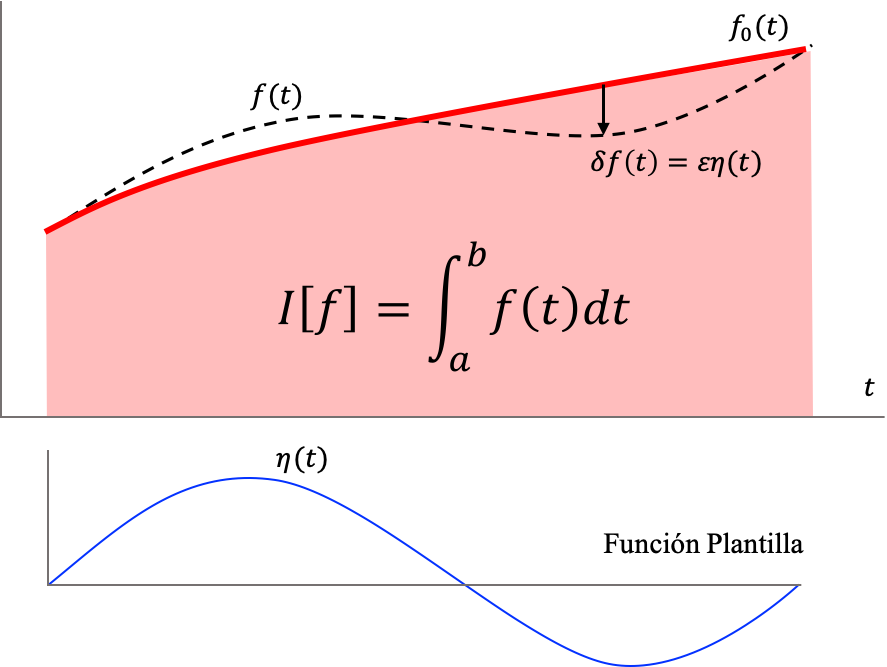
\includegraphics[width=0.7\textwidth]{./figures/horizontal_variacion_funcion.png}
\caption{El área bajo una curva es un funcional, en tanto depende de la
función que represente la curva, \(f(t)\) o \(f_0(t)\) Se conoce como
una variación \(\delta f\) a la diferencia entre dos funciones cercanas,
parametrizada a través de un número real \(\epsilon\) y una función
plantilla (panel inferior.) En términos de variaciones el valor de
cualquier función vecina a una función de referencia \(f_0\) se puede
calcular, en un intrevalo de interés, como
\(f(t)=f_0(t)+\epsilon\eta(t)\)
.\label{fig:variacion_funcion}}
\end{figure}

De la misma manera en la que se puede estudiar el efecto que un cambio
muy pequeño \(\Delta t\) en el valor de la variable independiente \(t\)
tiene en una función de variable real \(f(t)\), como lo hicimos por
ejemplo para definir la derivada (ver \autoref{derivadas}), en el
cálculo variacional es posible estudiar el efecto que un cambio pequeño
\(\delta f\) de una función \(f\) tiene en el funcional \(I[f]\)

Para hacerlo debemos primero definir otra función \(\eta\) que sirve de
``plantilla'' para el cambio. Al cambio en \(f\) se lo llama
\textbf{variación} y se escribe como:

\begin{equation}
\label{eq:variacion}
\delta f\equiv \epsilon \eta
\end{equation}

Una ilustración del concepto de \emph{variación} se muestra en la
\autoref{fig:variacion_funcion}. Allí reconocemos una importante
propiedad de la función de plantilla \(\eta(t)\) y es que vale cero en
los extremos del intervalo considerado \([a,b]\).

El cálculo variacional surgió originalmente para resolver problemas
prácticos en física, tales como hallar las funciones que máximan o
minimizan (extremos) funcionales de alguna utilidad.

Así por ejemplo, considere la siguiente pregunta: ¿cuál es la curva más
corta que conecta dos puntos en el plano de euclidiano?

Para responder a esta pregunta debemos primero construir el funcional
``distancia a lo largo de una curva'', también llamado, longitud de arco
(\cite{Apostol1969Calculus}):

\begin{equation}
\label{eq:longitud_curva}
I[f]=\int_a^b \sqrt{1+\left|\frac{\mathrm{d}f}{\mathrm{d}t}\right|^2}\;\mathrm{d}t
\end{equation}

Queremos encontrar la función \(f_0\) tal que \(I[f_0]\) tenga el mínimo
valor entre todas las posibles funciones \(f\).

Para encontrar la función que minimiza este funcional debemos, como se
acostumbra en el cálculo (\cite{Apostol1967Calculus}), derivar el
funcional respecto a la cantidad que parametriza la variación:
\(\epsilon\).

Escribamos el funcional de forma más general, en términos de una función
cercana al mínimo escrita como \(f=f_0+\epsilon\eta\):

\begin{equation}
\label{eq:funcional_integral}
I[f]=\int_a^b L(f(t),\dot{f}(t),t)\;\mathrm{d}t
\end{equation}

Nótese que hemos escrito el integrando como una función general \(L\)
que depende del valor de la función \(f(t)\), de su derivada
\(\dot{f}(t)\) y de la variable independiente \(t\). Implícitamente, el
funcional depende también del parámetro \(\epsilon\) dado que
\(f=f_0+\epsilon\eta\).

Si derivamos el funcional respecto de \(\epsilon\), obtenemos:

\[
\frac{\mathrm{d}I[f]}{\mathrm{d}\epsilon}=\int_a^b \frac{\mathrm{d}}{\mathrm{d}\epsilon} L(f(t),\dot{f}(t),t)\;\mathrm{d}t
\]

Aplicando la regla de la cadena, la integral del lado derecho nos queda:

\[
\frac{\mathrm{d}I[f]}{\mathrm{d}\epsilon}=\int_a^b 
\left(
\frac{\partial L}{\partial f}\frac{\mathrm{d}f}{\mathrm{d}\epsilon}+
\frac{\partial L}{\partial \dot{f}}\frac{\mathrm{d}\dot{f}}{\mathrm{d}\epsilon}
\right)
\;\mathrm{d}t
\]

Como \(f(t)=f_0(t)+\epsilon\eta(t)\), entonces
\(\mathrm{d}f/\mathrm{d}\epsilon=\eta\), mientras que
\(\mathrm{d}\dot{f}/\mathrm{d}\epsilon=\dot{\eta}\). Así la integral
anterior se desarrolla como:

\begin{equation}
\label{eq:dIdepsilon}
\frac{\mathrm{d}I[f]}{\mathrm{d}\epsilon}=\int_a^b 
\left(
\frac{\partial L}{\partial f}\eta+
\frac{\partial L}{\partial \dot{f}}\dot{\eta}
\right)
\;\mathrm{d}t
\end{equation}

El término
\(\int_a^b (\partial L/\partial \dot{f})\dot{\eta}\;\mathrm{d}t\) se
puede integrar por partes, si se hace \(u=\partial L/\partial \dot{f}\)
y \(\mathrm{d}v=\dot{\eta}\;\mathrm{d}t\):

\[
\int_a^b \frac{\partial L}{\partial \dot{f}}\dot{\eta}\;\mathrm{d}t=
\left.\frac{\partial L}{\partial \dot{f}}\eta\right|_a^b-
\int_a^b \frac{\mathrm{d}}{\mathrm{d}x}\left(\frac{\partial L}{\partial \dot{f}}\right)\eta\;\mathrm{d}t
\]

El primer término del lado derecho de la ecuación anterior es cero, en
tanto, por definición \(\eta(a)=\eta(b)=0\).

Reemplazando en la Ec. (\ref{eq:dIdepsilon}), la derivada del funcional
respecto de epsilon queda finalmente:

\[
\frac{\mathrm{d}I[f]}{\mathrm{d}\epsilon}=\int_a^b 
\eta(x)
\left(\frac{\partial L}{\partial f}-\frac{\mathrm{d}}{\mathrm{d}x}\frac{\partial L}{\partial \dot{f}}\right)
\;\mathrm{d}x
\]

Para que \(I[f]\) sea mínima en \(f=f_0\) su derivada
\(\mathrm{d}I[f]/{\mathrm{d}\epsilon}\) debe ser cero en \(\epsilon=0\).
Esto equivale a la \emph{ecuación integral}:

\begin{equation}
\label{eq:ecuacion_integral_variaciones}
\int_a^b 
\eta(x)
\left(\frac{\partial L}{\partial f}-\frac{\mathrm{d}}{\mathrm{d}t}\frac{\partial L}{\partial \dot{f}}\right)
\;\mathrm{d}t=0
\end{equation}

que lamentablemente no es muy útil para resolver nuestro problema
original. Para acercarnos a la solución necesitamos de un poderoso
teorema:
\begin{box_theorem}{Proposición}{}

\textbf{Lema fundamental del cálculo de variacions.} Si una función
continua \(f(t)\) en el intervalo abierto \((a,b)\) satisface la
igualdad:

\[
  \int_a^b f(t)h(t)\;\mathrm{d}t=0
  \]

para toda función \(h(t)\) continuamente diferenciable (todas sus
derivadas son continuas) y con \emph{soporte compacto} (acotada),
entonces \(f(t)=0\).

\end{box_theorem}
De acuerdo con este teorema, y suponiendo que \(\eta(t)\) es
continuamente diferenciable y acotada, la función entre paréntesis la
ecuación integral (\ref{eq:ecuacion_integral_variaciones}) es:

\begin{equation}
\label{eq:ecuacion_euler_lagrange}
\frac{\partial L}{\partial f}-\frac{\mathrm{d}}{\mathrm{d}t}\frac{\partial L}{\partial \dot{f}}=0
\end{equation}

Esta ecuación es una versión particular (para funciones de una sola
variable) de la que se conoce en la historia como la \textbf{ecuación de
Euler-Lagrange} y que será de importancia central en este libro.

Volviendo a nuestro problema original, es decir, encontrar la curva con
la menor longitud entre dos puntos, y reconociendo que:

\[
L(f(t),\dot{f}(t),t)=\sqrt{1+|\dot{f}(t)|^2},
\]

Entonces \(\partial L/\partial f=0\) (no aparece el símbolo \(f\) en la
fórmula de \(L\)) y
\(\partial L/\partial\dot{f}=\dot{f}/\sqrt{1+|\dot{f}(t)|^2}\). De allí,
la ecuación de Euler-Lagrange (\ref{eq:ecuacion_euler_lagrange}) en este
problema se convierte en:

\[
\frac{\mathrm{d}}{\mathrm{d}t}\left(\frac{\dot{f}}{\sqrt{1+|\dot{f}(t)|^2}}\right)=0
\]

Esta ecuación significa que el término entre paréntesis es constante.
Después de un poco de algebra, la expresión resultante, se puede
integrar para obtener:

\[
f(t)=At+B,
\]

donde \(A\), \(B\) son constantes.

La respuesta final a la pregunta original es ahora clara: la curva más
corta entre dos puntos en el plano euclidiano es una línea recta.

\hypertarget{algoritmos_calculo_variacional}{%
\subsubsection{Algoritmos en el cálculo
variacional}\label{algoritmos_calculo_variacional}}

Si el cálculo variacional es poco común en los textos básicos de cálculo
infinitesimal, los algoritmos relacionados con él son aún más escasos en
los textos de análisis numérico.

Dada la importancia del cálculo variacional en la mecánica nos
detendremos un momento aquí para explorar desde la algoritmia, al menos
la solución al problema de cálculo variacional que expusimos en la
sección anterior: el cálculo de la curva más corta entre dos puntos en
el plano euclidiano.

Para ello escribamos primero la rutina que servirá en nuestro caso como
funcional (y que implementa la Ec. \ref{eq:longitud_curva}):

    \begin{code}{Algoritmo}{code:funcional_integral}\begin{Verbatim}[fontsize=\small,commandchars=\\\{\}]
\PY{k}{def} \PY{n+nf}{funcional\PYZus{}integral}\PY{p}{(}\PY{n}{f0}\PY{p}{,}\PY{n}{eta}\PY{p}{,}\PY{n}{epsilon}\PY{p}{,}\PY{n}{a}\PY{p}{,}\PY{n}{b}\PY{p}{,}\PY{o}{*}\PY{o}{*}\PY{n}{opciones\PYZus{}de\PYZus{}f0}\PY{p}{)}\PY{p}{:}
    
    \PY{c+c1}{\PYZsh{}Definimos las función con su variación}
    \PY{n}{f}\PY{o}{=}\PY{k}{lambda} \PY{n}{t}\PY{p}{:}\PY{n}{f0}\PY{p}{(}\PY{n}{t}\PY{p}{,}\PY{o}{*}\PY{o}{*}\PY{n}{opciones\PYZus{}de\PYZus{}f0}\PY{p}{)}\PY{o}{+}\PY{n}{epsilon}\PY{o}{*}\PY{n}{eta}\PY{p}{(}\PY{n}{t}\PY{p}{)}
    
    \PY{c+c1}{\PYZsh{}La derivada de f la calculamos con derivative}
    \PY{k+kn}{from} \PY{n+nn}{scipy}\PY{n+nn}{.}\PY{n+nn}{misc} \PY{k}{import} \PY{n}{derivative}
    \PY{n}{dfdt}\PY{o}{=}\PY{k}{lambda} \PY{n}{t}\PY{p}{:}\PY{n}{derivative}\PY{p}{(}\PY{n}{f}\PY{p}{,}\PY{n}{t}\PY{p}{,}\PY{l+m+mf}{0.01}\PY{p}{)}
    
    \PY{c+c1}{\PYZsh{}Este es el integrando del funcional}
    \PY{k+kn}{from} \PY{n+nn}{numpy} \PY{k}{import} \PY{n}{sqrt}
    \PY{n}{L}\PY{o}{=}\PY{k}{lambda} \PY{n}{t}\PY{p}{:}\PY{n}{sqrt}\PY{p}{(}\PY{l+m+mi}{1}\PY{o}{+}\PY{n+nb}{abs}\PY{p}{(}\PY{n}{dfdt}\PY{p}{(}\PY{n}{t}\PY{p}{)}\PY{p}{)}\PY{o}{*}\PY{o}{*}\PY{l+m+mi}{2}\PY{p}{)}
    
    \PY{c+c1}{\PYZsh{}El funcional es la integral definida del integrando}
    \PY{k+kn}{from} \PY{n+nn}{scipy}\PY{n+nn}{.}\PY{n+nn}{integrate} \PY{k}{import} \PY{n}{quad}
    \PY{n}{integral}\PY{o}{=}\PY{n}{quad}\PY{p}{(}\PY{n}{L}\PY{p}{,}\PY{n}{a}\PY{p}{,}\PY{n}{b}\PY{p}{)}
    \PY{n}{longitud}\PY{o}{=}\PY{n}{integral}\PY{p}{[}\PY{l+m+mi}{0}\PY{p}{]}
    
    \PY{k}{return} \PY{n}{longitud}
\end{Verbatim}

%%

\end{code}

Nótese que un \emph{funcional} en el lenguaje de la algoritmia es una
rutina que recibe como parámetros otras rutina (en este caso \texttt{f0}
y \texttt{eta}) y devuelve un valor numérico (en este caso
\texttt{longitud}.)

La rutina en el Alg. (\ref{code:funcional_integral}), si bien parece
compleja, recoje todos los elementos que hemos aprendido en esta
sección: los parametros opcionales de una rutina expresados como
\texttt{**opciones\_de\_f0} y que vimos en una nota de la
\autoref{funciones}, las funciones \texttt{lambda} que vimos en la
misma sección, la derivada numérica calculada usando \texttt{derivative}
que conocimos en la \autoref{derivadas} y la integral por
cuadraturas usando \texttt{quad} de la \autoref{integrales}.

Más importante aún es el hecho que esta rutina puede usarse para
cualquier funcional que se exprese como una integral definida de la
forma de la Ec. (\ref{eq:funcional_integral}). Para adaptarla a otras
situaciones, simplemente se debe cambiar la función \texttt{L}. En la
sección de problemas al final de este capítulo se pone a prueba esta
rutina en otros contextos.

Supongamos ahora que queremos calcular la curva más corta que une los
puntos del plano cartesiano \((0,0)\) y \((\pi,1)\) (es decir \(a=0\) y
\(b=\pi\)). Para ello proponemos una función de referencia
\(f_0(t)=(t/\pi)^n\). Esta función para por ambos puntos para todo
\(n\). Como función de plantilla \(\eta(t)\), que debe ser una función
acotada de acuerdo al lema fundamental del cálculo de variaciones,
usaremos la función trigonométrica seno (que cumple la condición
\(\eta(a)=\sin 0=0\) y \(\eta(b)=\sin\pi=0\)).

El siguiente algoritmo implementa estas elecciones:

    \begin{code}{}{}\begin{Verbatim}[fontsize=\small,commandchars=\\\{\}]
\PY{c+c1}{\PYZsh{}Intevalo entre los puntos}
\PY{k+kn}{from} \PY{n+nn}{numpy} \PY{k}{import} \PY{n}{pi}
\PY{n}{a}\PY{o}{=}\PY{l+m+mi}{0}
\PY{n}{b}\PY{o}{=}\PY{n}{pi}

\PY{c+c1}{\PYZsh{}Funcion de referencia}
\PY{k}{def} \PY{n+nf}{curva}\PY{p}{(}\PY{n}{t}\PY{p}{,}\PY{n}{n}\PY{o}{=}\PY{l+m+mi}{1}\PY{p}{)}\PY{p}{:}
    \PY{k}{return} \PY{p}{(}\PY{n}{t}\PY{o}{/}\PY{n}{pi}\PY{p}{)}\PY{o}{*}\PY{o}{*}\PY{n}{n}

\PY{c+c1}{\PYZsh{}Función plantilla}
\PY{k+kn}{from} \PY{n+nn}{numpy} \PY{k}{import} \PY{n}{sin}
\PY{n}{eta}\PY{o}{=}\PY{n}{sin}
\end{Verbatim}

%%

\end{code}

Para ilustrar el uso de la rutina en el Alg.
(\ref{code:funcional_integral}), calculemos la longitud de arco para el
caso en el que \(n=2\) y \(\epsilon=0.5\):

    \begin{code}{}{}\begin{Verbatim}[fontsize=\small,commandchars=\\\{\}]
\PY{n}{n}\PY{o}{=}\PY{l+m+mi}{2}
\PY{n}{If}\PY{o}{=}\PY{n}{funcional\PYZus{}integral}\PY{p}{(}\PY{n}{curva}\PY{p}{,}\PY{n}{eta}\PY{p}{,}\PY{l+m+mf}{0.5}\PY{p}{,}\PY{n}{a}\PY{p}{,}\PY{n}{b}\PY{p}{,}\PY{n}{n}\PY{o}{=}\PY{n}{n}\PY{p}{)}
\end{Verbatim}

%%

\end{code}
\vspace{-1em}

%%hidecode


    \begin{Verbatim}[fontsize=\small,commandchars=\\\{\}]
I[f] = 3.337162809417341
\end{Verbatim}

Para encontrar la trayectoria más corta entre los puntos seleccionados,
debemos minimizar una función del tipo \texttt{longitud\_arco(epsilon)}
que llame a la rutina \texttt{funcional\_integral}, pero que solo
dependa de la variable que queremos minimizar, es decir de
\texttt{epsilon}. Para ello podemos definir la función \texttt{lambda}:

    \begin{code}{}{}\begin{Verbatim}[fontsize=\small,commandchars=\\\{\}]
\PY{n}{longitud\PYZus{}arco}\PY{o}{=}\PY{k}{lambda} \PY{n}{epsilon}\PY{p}{:}\PY{n}{funcional\PYZus{}integral}\PY{p}{(}\PY{n}{curva}\PY{p}{,}\PY{n}{eta}\PY{p}{,}\PY{n}{epsilon}\PY{p}{,}
                                                \PY{n}{a}\PY{p}{,}\PY{n}{b}\PY{p}{,}\PY{n}{n}\PY{o}{=}\PY{n}{n}\PY{p}{)}
\end{Verbatim}

%%

\end{code}

La minimización, finalmente, se consigue usando la rutina
\texttt{minimize} del paquete \texttt{SciPy}, capaz de encontar el
mínimo de funciones escalares con un número arbitario de variables. Lo
único que necesita \texttt{minimize} para lograr su cometido es que le
pasemos una rutina que tenga un solo parametro, en nuestro caso
\texttt{longitud\_arco} y un valor de prueba para la variable
independiente (en nuestro caso usaremos \(\epsilon=0\)):

    \begin{code}{Algoritmo}{code:minimiza_arco}\begin{Verbatim}[fontsize=\small,commandchars=\\\{\}]
\PY{k+kn}{from} \PY{n+nn}{scipy}\PY{n+nn}{.}\PY{n+nn}{optimize} \PY{k}{import} \PY{n}{minimize}
\PY{n}{solucion}\PY{o}{=}\PY{n}{minimize}\PY{p}{(}\PY{n}{longitud\PYZus{}arco}\PY{p}{,}\PY{l+m+mf}{0.0}\PY{p}{)}
\end{Verbatim}

%%

\end{code}
\vspace{-1em}

%%hidecode


    \begin{Verbatim}[fontsize=\small,commandchars=\\\{\}]
Resultado de la minimización:
      fun: 3.2975722013512403
 hess\_inv: array([[0.73687233]])
      jac: array([1.1920929e-06])
  message: 'Optimization terminated successfully.'
     nfev: 12
      nit: 3
     njev: 4
   status: 0
  success: True
        x: array([0.25801323])
\end{Verbatim}

Nótese que el resultado de la rutina \texttt{minimize} es un
\emph{objeto} entre cuyos atributos se encuentra el valor de la variable
independiente \texttt{x} que hace mínima la función de nuestro interés,
en este caso \texttt{longitud\_de\_arco}.

Puesto en términos de nuestro problema el resultado anterior indica que
para curvas del tipo \(f_0(t)=(t/\pi)^2\), que sufren variaciones con
una función plantilla \(\eta(t)=\sin t\), la curva de mínima longitud
entre el punto \((0,0)\) y el punto \((0,\pi)\), corresponde a una
variación con \(\epsilon=0.258\).

Hagamos un gráfico de la función resultante y de su comparación con la
solución analítica:
%%HIDE%%
    \begin{code}{Algoritmo}{code:4_Fundamentos_4}\begin{Verbatim}[fontsize=\small,commandchars=\\\{\}]
\PY{k+kn}{import} \PY{n+nn}{matplotlib}\PY{n+nn}{.}\PY{n+nn}{pyplot} \PY{k}{as} \PY{n+nn}{plt}
\PY{n}{plt}\PY{o}{.}\PY{n}{figure}\PY{p}{(}\PY{p}{)}

\PY{k+kn}{from} \PY{n+nn}{numpy} \PY{k}{import} \PY{n}{linspace}\PY{p}{,}\PY{n}{pi}
\PY{n}{ts}\PY{o}{=}\PY{n}{linspace}\PY{p}{(}\PY{l+m+mi}{0}\PY{p}{,}\PY{n}{pi}\PY{p}{)}

\PY{c+c1}{\PYZsh{}Valor de epsilon proveniende de la minimización}
\PY{n}{epsilon}\PY{o}{=}\PY{n}{solucion}\PY{o}{.}\PY{n}{x}\PY{p}{[}\PY{l+m+mi}{0}\PY{p}{]}

\PY{n}{plt}\PY{o}{.}\PY{n}{plot}\PY{p}{(}\PY{n}{ts}\PY{p}{,}\PY{n}{curva}\PY{p}{(}\PY{n}{ts}\PY{p}{,}\PY{n}{n}\PY{o}{=}\PY{n}{n}\PY{p}{)}\PY{p}{,}\PY{l+s+s1}{\PYZsq{}}\PY{l+s+s1}{r.}\PY{l+s+s1}{\PYZsq{}}\PY{p}{,}
         \PY{n}{label}\PY{o}{=}\PY{n}{f}\PY{l+s+s2}{\PYZdq{}}\PY{l+s+s2}{Curva de referencia}\PY{l+s+s2}{\PYZdq{}}\PY{p}{)}
\PY{n}{plt}\PY{o}{.}\PY{n}{plot}\PY{p}{(}\PY{n}{ts}\PY{p}{,}\PY{n}{curva}\PY{p}{(}\PY{n}{ts}\PY{p}{,}\PY{n}{n}\PY{o}{=}\PY{n}{n}\PY{p}{)}\PY{o}{+}\PY{n}{epsilon}\PY{o}{*}\PY{n}{eta}\PY{p}{(}\PY{n}{ts}\PY{p}{)}\PY{p}{,}\PY{l+s+s1}{\PYZsq{}}\PY{l+s+s1}{b\PYZhy{}}\PY{l+s+s1}{\PYZsq{}}\PY{p}{,}
         \PY{n}{label}\PY{o}{=}\PY{n}{f}\PY{l+s+s2}{\PYZdq{}}\PY{l+s+s2}{Curva variada con \PYZdl{}}\PY{l+s+s2}{\PYZbs{}}\PY{l+s+s2}{epsilon\PYZdl{}=}\PY{l+s+si}{\PYZob{}epsilon:g\PYZcb{}}\PY{l+s+s2}{\PYZdq{}}\PY{p}{)}
\PY{n}{plt}\PY{o}{.}\PY{n}{plot}\PY{p}{(}\PY{n}{ts}\PY{p}{,}\PY{n}{curva}\PY{p}{(}\PY{n}{ts}\PY{p}{,}\PY{n}{n}\PY{o}{=}\PY{l+m+mi}{1}\PY{p}{)}\PY{p}{,}\PY{l+s+s1}{\PYZsq{}}\PY{l+s+s1}{k\PYZhy{}\PYZhy{}}\PY{l+s+s1}{\PYZsq{}}\PY{p}{,}
         \PY{n}{label}\PY{o}{=}\PY{n}{f}\PY{l+s+s2}{\PYZdq{}}\PY{l+s+s2}{Línea recta}\PY{l+s+s2}{\PYZdq{}}\PY{p}{)}

\PY{n}{plt}\PY{o}{.}\PY{n}{legend}\PY{p}{(}\PY{p}{)}\PY{p}{;}

\PY{c+c1}{\PYZsh{}\PYZhy{}\PYZhy{}hide\PYZhy{}\PYZhy{}}
\PY{n}{plt}\PY{o}{.}\PY{n}{xlabel}\PY{p}{(}\PY{l+s+s2}{\PYZdq{}}\PY{l+s+s2}{t}\PY{l+s+s2}{\PYZdq{}}\PY{p}{)}\PY{p}{;}
\end{Verbatim}

%%figcaption::show::La curva continua indica una aproximación numérica al camino más corto entre los puntos $(0,0)$ y $(0,\pi)$ del plano euclidiano, encontrada al minimizar el funcional longitud de arco y usando como función de prueba $f_0=(t/\pi)^n$ (linea punteada) y como función plantilla $\epsilon(t)=\sin t$.  El valor de $\epsilon$ que corresponde a la solución se muestra en la etiqueta.  Para comparación se muestra (linea rayada) la solución exacta, que corresponde a una línea recta.

\tcblower
\footnotesize
\em ver Figura \ref{fig:code:4_Fundamentos_4}
\end{code}

    \begin{center}

\begin{figure}[ht!]
\centering
    \adjustimage{max size={0.8\linewidth}{0.8\paperheight}}{combined_files/combined_248_0.png}
\caption{Figura correspondiente al código \ref{code:4_Fundamentos_4}. La curva continua indica una aproximación numérica al camino más corto entre los puntos $(0,0)$ y $(0,\pi)$ del plano euclidiano, encontrada al minimizar el funcional longitud de arco y usando como función de prueba $f_0=(t/\pi)^n$ (linea punteada) y como función plantilla $\epsilon(t)=\sin t$.  El valor de $\epsilon$ que corresponde a la solución se muestra en la etiqueta.  Para comparación se muestra (linea rayada) la solución exacta, que corresponde a una línea recta.\label{fig:code:4_Fundamentos_4}}
\end{figure}

    \end{center}
%{ \hspace*{\fill} \\}
    
\hypertarget{graficos_interactivos_variacional}{%
\subsection{Gráficos
interactivos}\label{graficos_interactivos_variacional}}

Para ver los gráficos interactivos use a las libretas de
\texttt{Jupyter} que que están disponibles en la versión electrónica del
libro.



\hypertarget{conicas}{%
\section{Curvas cónicas}\label{conicas}}

En el año 1609, Johannes Kepler descubrió uno de los secretos mejor
guardados del Universo: el camino que seguía el planeta Marte alrededor
del Sol no era un círculo, como lo ``mandaban'' siglos de tradición
filósofica y astronómica, sino una \emph{elipse}.

Durante meses el astrónomo Prusiano había estado luchando, sin mucha
suerte, por ajustar las precisas observaciones del astrónomo Danés Tycho
Brahe (\hreffoot{https://es.forvo.com/word/tycho_brahe}{``tico braja''}) del
planeta en cuestión, al modelo que Nicolás Copernico había desarrollado
unos 60 años antes y en el que se suponía que los planetas se movían
``alrededor'' del Sol sobre trayectorias circulares descentradas (el Sol
no ocupaba realmente el centro en el sistema Copernicano.)

Después de muchos intentos fallidos Kepler relata, en la que hoy se
considera su obra cumbre ``\emph{Astronomía Nueva}'', que desesperado
empezó a considerar la posibilidad de que la órbita de Marte fuera
``ovalada'' (con forma de huevo) en lugar de circular. Finalmente,
después de muchos intentos, Kepler ``adivinó'' que el ovalo no podía ser
otra cosa sino una elipse, una figura geométrica que había sido
ampliamente estudiada por los geómetras de la antigüedad y la edad
media, pero cuyo papel en la astronomía no había sido considerado hasta
ese momento.

Esta historia marco el inició de la mecánica celeste y el renacimiento
del interés astronómico por la elipse y las curvas emparentadas con ella
y que hoy llamamos \emph{curvas cónicas}. En las próximas sesiones
repasaremos las propiedades geométricas de las cónicas, desde su
definición original hasta su descripción algebraica moderna, en
preparación para su aplicación en el estudio de la trayectoria de los
cuerpos en mecánica celeste.

\hypertarget{conicas_definicion}{%
\subsection{Definición geométrica}\label{conicas_definicion}}

Desde los primeros trabajos geométricos griegos, compilados y
organizados por Euclides de Alejandría (323 a 283 a.e.c.) en su libro
``\emph{Elementos}'', se sabe que la familia de curvas que resultan de
intersectar un plano con un cono (una figura que se forma al hacer rotar
en el espacio un triángulo alrededor de uno de sus lados, ver
\autoref{fig:conica_definicion}) tienen propiedades geométricas
especiales. Es a esta familia curvas a las que llamamos \emph{cónicas},
en clara referencia a su definición geométrica original.

\begin{figure}[t!]
\centering
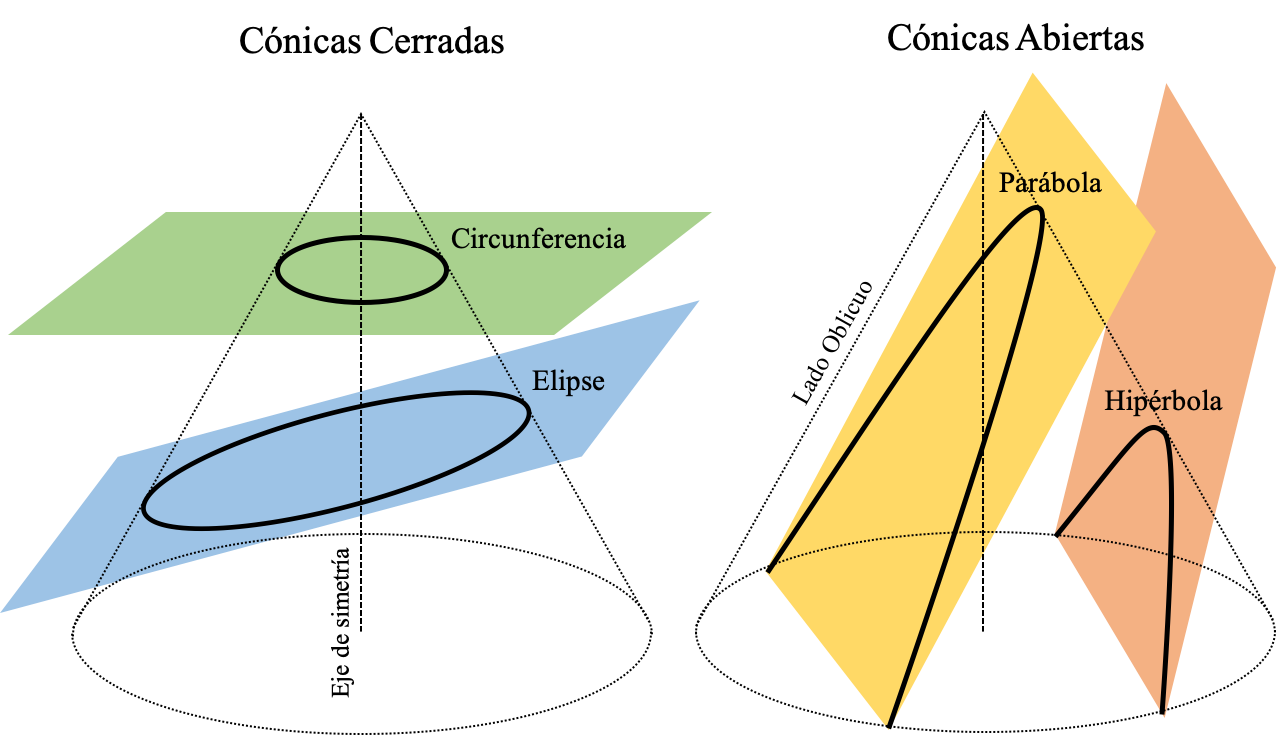
\includegraphics[width=0.8\textwidth]{./figures/horizontal_conicas.png}
\caption{Definición geométrica original de las \emph{curvas
cónicas}.\label{fig:conicas_definicion}}
\end{figure}

La \textbf{circunferencia}, que es una cónica, resulta por ejemplo de
intersectar el cono con un plano perpendicular a su eje de simetría. Si
el plano, sin embargo, forma un ángulo distinto de 90 grados con el eje
de simetría, pero no es paralelo a los lados del cono, la figura
resultante, que es también cerrada como la circunferencia, se llama una
\textbf{elipse}. Si el plano es paralelo a los lados oblicuos del cono
la figura resultante es abierta y la llamamos una \textbf{parábola}.
Finalmente, si el plano no es paralelo a los lados del cono, pero por su
ángulo nunca intersecta el eje de simetría, decimos que la figura que se
forma es una \textbf{hipérbola}.

\hypertarget{conicas_nombre_algebra}{%
\subsection{Del nombre al álgebra}\label{conicas_nombre_algebra}}

La palabra ``parábola'' viene del griego
\(\pi\alpha\rho\alpha\beta\alpha\lambda\lambda\epsilon\iota\nu\)
(``parabalei'') que significa ``poner al lado'', ``igualar'',
``comparar'' (de allí que una parábola en español sea también una
historia que donde se narran hechos que pueden servir como modelos de
comportamiento.) Este curioso nombre tiene su origen en la manera como
este tipo de curva fue definida de forma más rigurosa a como lo hicimos
en la sección anterior, por uno de los más grandes matemáticos de la
antiguedad, Apolonio de Perga (ca. 262 a ca. 190 a.e.c.) en su tratado
clásico \emph{Conicas}.

En la \autoref{fig:conicas_apolonio} se ilustra la construcción de
Apolonio y la razón para el nombre que dió a cada cónica. Para ello
ubicamos las curvas sobre el plano de modo que su eje de simetría quede
alineado con una semirrecta horizontal que comienza en el punto O que
llamaremos \emph{apside} de la cónica (la elipse tiene dos
\emph{apsides}.) Todas las cónicas de la figura tienen asociado un
parámetro que define su tamaño y que es igual a la longitud de un
segmento \(\overline{\mathrm{OR}}\) perpendicular al eje de simetría. Si
aumentamos o disminuímos la longitud de este segmento las cónicas serán
más grandes o más pequeñas de las representadas en la figura. Por cada
punto P de las cónicas existe un punto Q que es su proyección sobre el
eje de simetría.

\begin{figure}[t!]
\centering
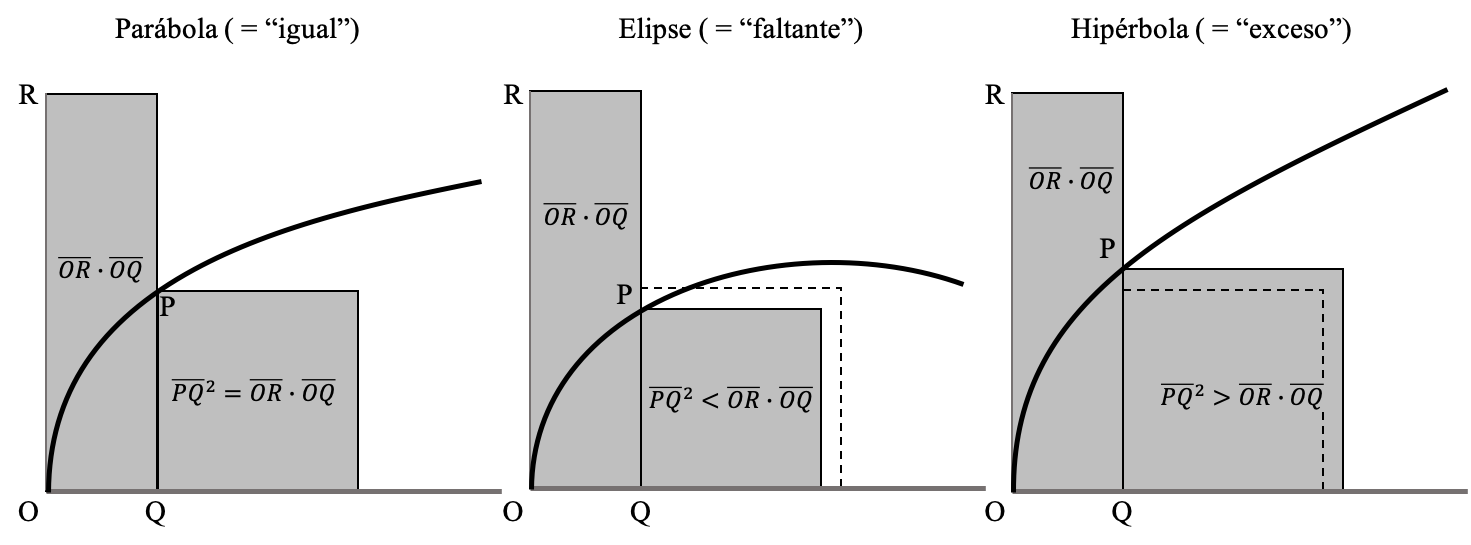
\includegraphics[width=1.0\textwidth]{./figures/horizontal_conicas_apolonio.png}
\caption{Definición con \emph{áreas aplicadas} de las \emph{curvas
cónicas} y el origen de sus
nombres.\label{fig:conicas_apolonio}}
\end{figure}

La propiedad descubierta por Apolonio (y posiblemente por Euclides y
otros matemáticos anteriores a él) es que el área del rectángulo que
tiene como base el segmento \(\overline{\mathrm{OQ}}\) y como altura el
parámetro de tamaño, es decir, la longitud del segmento
\(\overline{\mathrm{OR}}\) puede ser (dependiendo de la cónica) igual,
menor o mayor al área del cuadrado que tiene como lado la longitud del
segmento \(\overline{\mathrm{PQ}}\). En la geometría clásica a esta
operación se la llama la \emph{aplicación de un rectángulo} o la
\emph{cuadratura del rectángulo}.

La parábola es entonces la figura en la que esas áreas son exactamente
iguales. De allí su nombre en griego. Por otra parte la elipse, cuyo
nombre viene del griego
\(\epsilon\lambda\epsilon\iota\pi\epsilon\iota\nu\) (``eleipeín'') que
significa ``faltante'', es tal que el área del cuadrado no alcanza a ser
igual a la del rectángulo. Y en la hipérbola, cuyo nombre viene del
griego \(\nu\pi\epsilon\rho\beta\alpha\lambda\lambda\epsilon\iota\nu\)
(``hiperbalein'') que significa ``exceso'', el área del cuadrado supera
la del rectángulo aplicado.

En términos algebraicos (geometría analítica), si construímos un sistema
de coordenadas cartesianas con origen en el ápside O, eje \(x_a\) (el
subíndice indica precisamente que el origen esta en al apside) en la
dirección del eje de simetría y eje \(y_a\) en dirección del semgento
\(\overline{\mathrm{OR}}\) (cuya longitud llamamremos \(L\)), las
coordenadas \((x_a,y_a)\) de los puntos sobre las cónicas se relacionan
de acuerdo con \cite{Eves1972Geometry}:

\begin{equation}
\label{eq:ecuacion_apside}
y_a^2 = Lx_a+\eta x_a^2 
\end{equation}

Aquí \(\eta\) es un parámetro que define la ``forma'' de la cónica,
siendo:

\begin{itemize}
\tightlist
\item
  \(\eta=0\) en el caso de un \textbf{parábola}.
\item
  \(\eta<0\) en el caso de una \textbf{elipse}.
\item
  \(\eta>0\) en el caso de una \textbf{hipérbola}.
\end{itemize}

Por su origen llamaremos a \(\eta\) el parámetro de Apolonio de la
cónica.

En el algoritmo a continuación usamos estas definiciones para dibujar
las cónicas y ver el efecto que tienen los parámetros \(L\) y \(\eta\)
en su tamaño y forma.
%%HIDE%%
    \begin{code}{Algoritmo}{code:4_Fundamentos_5}\begin{Verbatim}[fontsize=\small,commandchars=\\\{\}]
\PY{c+c1}{\PYZsh{}Definimos el algoritmo como una rutina}
\PY{k}{def} \PY{n+nf}{conicas\PYZus{}apolonio}\PY{p}{(}\PY{n}{eta}\PY{o}{=}\PY{o}{\PYZhy{}}\PY{l+m+mf}{0.5}\PY{p}{)}\PY{p}{:}

    \PY{c+c1}{\PYZsh{}Escala}
    \PY{n}{L}\PY{o}{=}\PY{l+m+mf}{10.0}
    \PY{c+c1}{\PYZsh{}Forma}
    \PY{n}{eta}\PY{o}{=}\PY{n+nb}{float}\PY{p}{(}\PY{n}{eta}\PY{p}{)}
    
    \PY{c+c1}{\PYZsh{}Máximo valor de x}
    \PY{n}{xamax}\PY{o}{=}\PY{n}{L}\PY{o}{/}\PY{n+nb}{abs}\PY{p}{(}\PY{n}{eta}\PY{p}{)} \PY{k}{if} \PY{n+nb}{abs}\PY{p}{(}\PY{n}{eta}\PY{p}{)}\PY{o}{\PYZgt{}}\PY{l+m+mi}{0} \PY{k}{else} \PY{n}{L}
    
    \PY{c+c1}{\PYZsh{}Valores de x en los que graficaremos}
    \PY{k+kn}{from} \PY{n+nn}{numpy} \PY{k}{import} \PY{n}{sqrt}\PY{p}{,}\PY{n}{linspace}
    \PY{n}{xas}\PY{o}{=}\PY{n}{linspace}\PY{p}{(}\PY{l+m+mi}{0}\PY{p}{,}\PY{n}{xamax}\PY{p}{,}\PY{l+m+mi}{100}\PY{p}{)}

    \PY{c+c1}{\PYZsh{}Ecuaciones de las cónicas referidas al apside}
    \PY{k+kn}{from} \PY{n+nn}{numpy} \PY{k}{import} \PY{n}{append}
    \PY{n}{yas\PYZus{}par}\PY{o}{=}\PY{n}{sqrt}\PY{p}{(}\PY{n}{L}\PY{o}{*}\PY{n}{xas}\PY{p}{)}
    \PY{n}{yas}\PY{o}{=}\PY{n}{sqrt}\PY{p}{(}\PY{n}{L}\PY{o}{*}\PY{n}{xas}\PY{o}{+}\PY{n+nb}{float}\PY{p}{(}\PY{n}{eta}\PY{p}{)}\PY{o}{*}\PY{n}{xas}\PY{o}{*}\PY{o}{*}\PY{l+m+mi}{2}\PY{p}{)}

    \PY{c+c1}{\PYZsh{}Gráfica}
    \PY{k+kn}{import} \PY{n+nn}{matplotlib}\PY{n+nn}{.}\PY{n+nn}{pyplot} \PY{k}{as} \PY{n+nn}{plt}
    \PY{n}{fig}\PY{o}{=}\PY{n}{plt}\PY{o}{.}\PY{n}{figure}\PY{p}{(}\PY{n}{figsize}\PY{o}{=}\PY{p}{(}\PY{l+m+mi}{6}\PY{p}{,}\PY{l+m+mi}{6}\PY{p}{)}\PY{p}{)}
    \PY{n}{ax}\PY{o}{=}\PY{n}{fig}\PY{o}{.}\PY{n}{gca}\PY{p}{(}\PY{p}{)}

    \PY{n}{ax}\PY{o}{.}\PY{n}{plot}\PY{p}{(}\PY{n}{xas}\PY{p}{,}\PY{n}{yas\PYZus{}par}\PY{p}{,}\PY{l+s+s1}{\PYZsq{}}\PY{l+s+s1}{k\PYZhy{}\PYZhy{}}\PY{l+s+s1}{\PYZsq{}}\PY{p}{)}
    \PY{n}{ax}\PY{o}{.}\PY{n}{plot}\PY{p}{(}\PY{n}{xas}\PY{p}{,}\PY{o}{\PYZhy{}}\PY{n}{yas\PYZus{}par}\PY{p}{,}\PY{l+s+s1}{\PYZsq{}}\PY{l+s+s1}{k\PYZhy{}\PYZhy{}}\PY{l+s+s1}{\PYZsq{}}\PY{p}{)}
    \PY{n}{ax}\PY{o}{.}\PY{n}{plot}\PY{p}{(}\PY{n}{xas}\PY{p}{,}\PY{n}{yas}\PY{p}{,}\PY{l+s+s1}{\PYZsq{}}\PY{l+s+s1}{b}\PY{l+s+s1}{\PYZsq{}}\PY{p}{)}
    \PY{n}{ax}\PY{o}{.}\PY{n}{plot}\PY{p}{(}\PY{n}{xas}\PY{p}{,}\PY{o}{\PYZhy{}}\PY{n}{yas}\PY{p}{,}\PY{l+s+s1}{\PYZsq{}}\PY{l+s+s1}{b}\PY{l+s+s1}{\PYZsq{}}\PY{p}{)}

    \PY{c+c1}{\PYZsh{}Decoración}
    \PY{n}{ax}\PY{o}{.}\PY{n}{grid}\PY{p}{(}\PY{p}{)}
    \PY{n}{ax}\PY{o}{.}\PY{n}{set\PYZus{}title}\PY{p}{(}\PY{n}{f}\PY{l+s+s2}{\PYZdq{}}\PY{l+s+s2}{Cónica con \PYZdl{}L = }\PY{l+s+si}{\PYZob{}L\PYZcb{}}\PY{l+s+s2}{\PYZdl{}, \PYZdl{}}\PY{l+s+s2}{\PYZbs{}}\PY{l+s+s2}{eta=}\PY{l+s+si}{\PYZob{}eta\PYZcb{}}\PY{l+s+s2}{\PYZdl{}}\PY{l+s+s2}{\PYZdq{}}\PY{p}{)}
    
    \PY{c+c1}{\PYZsh{}Fijamos la misma escala en los ejes}
    \PY{k+kn}{from} \PY{n+nn}{pymcel}\PY{n+nn}{.}\PY{n+nn}{plot} \PY{k}{import} \PY{n}{fija\PYZus{}ejes\PYZus{}proporcionales}
    \PY{n}{valores}\PY{o}{=}\PY{p}{(}\PY{n}{xas}\PY{p}{,}\PY{n}{yas\PYZus{}par}\PY{p}{,}\PY{o}{\PYZhy{}}\PY{n}{yas\PYZus{}par}\PY{p}{,}\PY{n}{yas}\PY{p}{,}\PY{o}{\PYZhy{}}\PY{n}{yas}\PY{p}{)}\PY{p}{,}
    \PY{n}{fija\PYZus{}ejes\PYZus{}proporcionales}\PY{p}{(}\PY{n}{ax}\PY{p}{,}\PY{n}{valores}\PY{p}{,}
                             \PY{n}{xmin}\PY{o}{=}\PY{o}{\PYZhy{}}\PY{n}{xamax}\PY{o}{/}\PY{l+m+mi}{2}\PY{p}{,}\PY{n}{ycm}\PY{o}{=}\PY{l+m+mi}{0}\PY{p}{)}\PY{p}{;}
    
\PY{c+c1}{\PYZsh{}Invocamos la rutina}
\PY{n}{conicas\PYZus{}apolonio}\PY{p}{(}\PY{p}{)}
\end{Verbatim}

%%

\tcblower
\footnotesize
\em ver Figura \ref{fig:code:4_Fundamentos_5}
\end{code}

    \begin{center}

\begin{figure}[ht!]
\centering
    \adjustimage{max size={0.8\linewidth}{0.8\paperheight}}{combined_files/combined_267_0.png}
\caption{Figura correspondiente al código \ref{code:4_Fundamentos_5}.\label{fig:code:4_Fundamentos_5}}
\end{figure}

    \end{center}
%{ \hspace*{\fill} \\}
    
Trate de demostrar usando el algoritmo o manipulando la Ec.
(\ref{eq:ecuacion_apside}) que la circunferencia, que en la definición
original se considera una cónica más, no es más que una elipse para la
cuál el parámetro de forma \(\eta\) es igual a -1.

Para ver esta una versión interactiva de esta figura por favor use las
libretas disponibles en la
\hreffoot{http://seap-udea.org/MecanicaCeleste_Zuluaga}{versión electrónica
del libro}.
%%HIDE%%
\hypertarget{conicas_directriz}{%
\subsection{Directriz de las cónicas}\label{conicas_directriz}}

La definición de Apolonio de las cónicas provista en la sección
anterior, no solo nos permite introducir la primera fórmula algebraica
para describirlas (Ec. \ref{eq:conicas_apolonio}) y tal vez la primera
en la historia que lo hizo, sino que además nos ayudó a entender el
origen de sus nombres.

Sin embargo, esta definición adolece de algunas características que nos
resultaran muy útiles en lo sucesivo. No es claro, por ejemplo, la
relación entre los parámetros de tamaño \(L\) y forma \(\eta\) con otras
propiedades de la cónica (en el caso de una elipse por ejemplo con su
diámetro.)

Una definición más conveniente es la de Arquímedes (introducida
posiblemente unos años antes que Apolonio y usada más frecuentemente en
la edad media y tiempos modernos.) Esta definición se basa en
proporciones más que en áreas.

\begin{figure}[ht!]
\centering
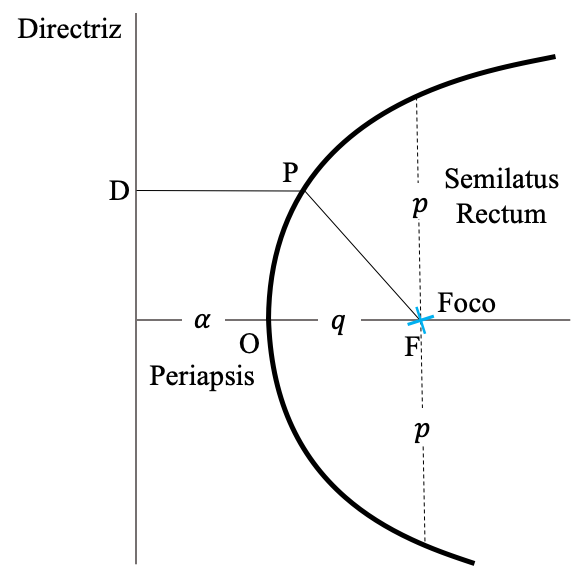
\includegraphics[width=0.5\textwidth]{./figures/square_conicas_directriz.png}
\caption{Definición de las cónicas usando la recta directriz y el
foco.\label{fig:conicas_directriz}}
\end{figure}

Según esta definición, toda cónica se puede construir partiendo de una
recta a la que se llama \emph{recta directriz} y un punto o \emph{foco}
(ver \autoref{fig:conicas_directriz}.) Las cónicas son el lugar
geométrico de los puntos tal que la razón de la distancia del punto al
foco y la distancia del punto a la directriz es constante:

\begin{equation}
\label{eq:conica_razon}
 \displaystyle \frac{\overline{PF}}{\overline{PD}}\equiv e
\end{equation} donde \(e>0\). A este parámetro lo llamamos la
\emph{excentricidad} de la cónica.

Si definimos un sistema de coordenadas tal que el eje \(y_d\) pase por
la recta directríz (el subíndice \(d\) indica que el sistema de
coordenadas esta precisamente referido a la directriz) y el eje \(x_d\)
por el foco, en términos de las coordenadas \((x_d,y_d)\) de cada punto
de la cónica, la condición en la Ec. (\ref{eq:conica_razon}) se puede
escribir como:

\begin{equation}
\label{eq:conica_razon_cartesianas}
\frac{\sqrt{(F-x_d)^2+y_d^2}}{x_d}=e
\end{equation} donde \(F\) es la distancia del Foco a la directriz.

Despejando \(y\) obtenemos:

\begin{equation}
\label{eq:ecuacion_directriz}
y_d^2=(e^2-1) x_d^2 + 2F x_d - F^2
\end{equation}

Una comparación de esta ecuación con la Ec. (\ref{eq:ecuacion_apside})
revela inmediatamente que el valor de la excentricidad dependerá de la
cónica así:

\begin{itemize}
\tightlist
\item
  \(e=1\) en el caso de la \textbf{parábola}.
\item
  \(0<e<1\) en el caso de de una \textbf{elipse}.
\item
  \(e>1\) en el caso de una \textbf{hipérbola}.
\end{itemize}

Estudiemos ahora la posición de dos puntos sobre la cónica que merecen
alguna atención. El primero es el punto que se encuentra justo encima
del foco, es decir \(x=F\). La distancia vertical del eje de simetría a
este punto se conoce como el \emph{semilatus rectum} y se denota como
\(p\). Reemplazando en la Ec. (\ref{eq:ecuacion_directriz}):

\[
p^2=(e^2-1)F^2+2F^2-F^2
\] de donde se obtiene:

\[
p=eF
\]

El otro punto es el apside más cercano a la directriz. Si llamamos
\(\alpha\) a la distancia de ese punto a la directriz y usamos la
definición de la cónica en la Ec. (\ref{eq:conica_razon_cartesianas})
obtenemos:

\begin{equation}
\label{eq:alpha}
\alpha=\frac{F}{1+e}
\end{equation}

Por otro lado la distancia del foco al apside más cercano, que
llamaremos \textbf{periapsis} \(q\), viene dada en términos de \(F\),
\(e\) por:

\[
\begin{array}{rcl}
q & = & F-\alpha \\
  & = & eF/(1+e) \\
\end{array}
\] o bien,

\begin{equation}
\label{eq:q}
q=\frac{p}{1+e}
\end{equation}

Si trasladamos ahora la Ec. (\ref{eq:ecuacion_directriz}) el origen de
coordenadas en el punto O, es decir si reemplazamos \(x_d=x_a+\alpha\),
\(y_d=y_a\) obtenemos:

\begin{equation}
\label{eq:ecuacion_directriz_trasladada}
y_a^2 = 2 e F x_a + (e^2-1) x_a^2
\end{equation} que comparando con la Ec. (\ref{eq:ecuacion_apside}) nos
permite escribir los parámetros de tamaño \(L\) y forma \(\eta\) en la
definición de Apolonio, en función de la excentricidad \(e\) y
\emph{semilatus rectum} \(p\):

\[
L = 2p\\
\]

\begin{equation}
\label{eq:eta_apolonio}
\eta = e^2-1
\end{equation}

De esta última relación y de la frase final de la
\autoref{conicas_nombre_algebra} en la que identificamos a la
circunferencia como la cónica con \(\eta=-1\), concluimos nuevamente que
la circunferencia no es más que una elipse para la cuál \(e=0\).

\hypertarget{conicas_sintesis_geometrica}{%
\subsection{Síntesis geométrica}\label{conicas_sintesis_geometrica}}

En resumen podemos decir que las curvas cónicas, o al menos sus
principios de construcción, eran conocidas en Grecia posiblemente desde
el tiempo de los pitagóricos. Sin embargo, fue Apolonio de Perga quién
profundizo en las propiedades geométricas y ``algebraicas'' de estas
curvas. Su aplicación astronómica, sin embargo, era desconocida y fue
descubierta solo hasta los trabajos de Kepler en los 1600.

En términos geométricos simples las cónicas con el resultado de la
intersección de un cono con un plano con cuatro posibles inclinaciones
respecto a su eje de simetría. A pesar de que esto implicaría que
existen cuatro posibles cónicas, las definiciones posteriores demuestran
que en realidad la circunferencia es un caso particular de la elipse
(\(\eta=-1\) o \(e=0\).)

Toda cónica tiene: un eje de simetría, una recta directriz, un foco, un
ápside (el periapsis o punto más cercano al foco) y un \emph{latus
rectum} (segmento perpendicular al eje y que pasa por el foco.) Las
elipses tienen un segundo eje de simetría, perpendicular al primero y a
distancias iguales de dos apsides y por la misma razón un segundo foco y
un segundo \emph{latus rectum}.

Las dimensiones y forma de una cónica se pueden describir, en general,
en términos de dos parámetros:

\begin{itemize}
\item
  \textbf{Parametrización de Apolonio}. Los parámetros son la longitud
  del \emph{latus rectum} \(L>0\) y el parámetro de Apolonio
  \(-\infty<\eta<\infty\). De acuerdo con \(\eta\) las cónicas se
  clasifican en: parábola (\(\eta=0\)), circunferencia o elipse
  (\(\eta<0\)) e hipérbola (\(\eta>0\)).
\item
  \textbf{Parametrización de Arquímedes}. Los parámetros son el
  \emph{semilatus rectum} \(p>0\) y la excéntricidad \(0\leq e<1\). De
  acuerdo con \(e\) las cónicas se clasifican en: parábola (\(e=1\)),
  circunferencia y elipse (\(0\leq e<1\)) e hipérbola (\(e>1\)).
\end{itemize}

Se acostumbra usar más la parametrización de Arquímedes y es la que
utilizaremos en lo sucesivo en el libro.

Si se construye un sistema de coordenadas en el plano de la cónica, con
eje \(x\) en la dirección del eje de simetría, dependiendo de la
localización del origen, las coordenadas cartesianas de los puntos sobre
la cónica obedecen las ecuaciones:

\begin{itemize}
\tightlist
\item
  \textbf{Origen en el ápside}: \(y_a^2 = 2p x_a + (e^2-1) x_a^2\).
\item
  \textbf{Origen en la directriz}:
  \(y_d^2 = (e^2-1) x_d^2 + (2p/e) x_d - (p/e)^2\)
\end{itemize}

Esta última ecuación no es conveniente para describir la circunferencia.



\hypertarget{conicas_algebra}{%
\subsection{Descripción algebraica}\label{conicas_algebra}}

Si bien en las secciones anteriores adscribimos a Apolonio y a
Arquímedes (y a sus contemporáneos griegos) la descripción de las
cónicas en términos de ecuaciones algebraicas con sus coordenadas como
variables, en realidad esta descripción solo apareció en la historia con
el surgimiento de la moderna Geometría analítica en los 1600 y de la
mano de René Descartes
(\hreffoot{https://es.forvo.com/word/ren\%C3\%A9_descartes/\#fr}{``René
decart''}) y Pierre de Fermat (``pier de fermat'').

Ahora bien, la forma algebraica general que vimos en la Ec.
(\ref{eq:ecuacion_apside})

\begin{equation}
\label{eq:ecuacion_apside_pe}
y_a^2-2p x_a -(e^2-1) x_a^2 = 0
\end{equation} no es precisamente ni la fórmula más simple, ni la más
general.

En esta sección exploraremos a fondo las propiedades algebraicas de las
cónicas y al hacerlo descubriremos algunas propiedades importantes que
usaremos en la mecánica celeste.

Si queremos escribir la ecuación de la cónica en otras formas, podemos,
como lo hicimos en el caso de la Eq.
\ref{eq:ecuacion_directriz_trasladada}, aplicar dos tipos de
transformaciones al sistema de coordenadas:

\begin{itemize}
\item
  Una \textbf{traslación}, que implica simplemente modificar la posición
  del origen de coordenadas, tal y como hicimos en la
  \autoref{conicas_directriz} al pasar del origen en la directriz a
  un origen en el ápisde.
\item
  Una \textbf{rotación}, que implica modificar la dirección de los ejes
  coordenados. Esta es una transformación más compleja pero que
  resultará particularmente útil en la aplicación de las cónicas en
  mecánica celeste.
\end{itemize}

\hypertarget{conicas_centro}{%
\subsection{Ecuación respecto al centro}\label{conicas_centro}}

Para encontrar una forma más simple de la ecuación de la cónica, podemos
realizar una traslación del origen, del apside (respecto al cuál esta
escrita la Ec. \ref{eq:ecuacion_apside}) a un punto C en el cuál la
forma algebraica, por ejemplo solo contenga términos cuadráticos en las
coordenadas.

Una traslación a lo largo del eje \(x\) se escribe como:

\begin{eqnarray}
\label{eq:traslacion_centro}
x_a & = & x_c + a \\
\nonumber
y_a & = & y_c  
\end{eqnarray} donde \(a\) es la distancia del origen de las nuevas
coordenadas \(x_c,y_c\) (punto C), al origen de las coordenadas
\(x_a,y_a\) (apside).

Reemplazando las Ecs. (\ref{eq:traslacion_centro}) en la ecuación de la
cónica obtenemos:

\[
y_a^2-2p(x_c+a)+(1-e^2)(x_c+a)^2=0
\] que después de una manipulación algebraica se puede escribir en la
forma:

\[
y_c^2+(1-e^2)x_c^2+2[(1-e^2)a-p]x_c=2pa-(1-e^2)a^2
\]

Como el valor de \(a\) es libre, podemos escogerlo de modo el término
lineal en \(x_c\) desaparezca. Con esta elección el valor de esta
constante queda:

\begin{equation}
\label{eq:semiejemayor}
a=\frac{p}{1-e^2}
\end{equation}

Descubrimos aquí que el desplazamiento al punto \(C\) solo tiene el
efecto deseado en el caso en el que \(e\neq 1\) (elipse e hipérbola).
Para el caso de la parábola, en realidad la forma más simple de la
ecuación sigue siendo aquella referida al apside (Ec.
\ref{eq:ecuacion_apside}), \(y_d^2=2px_d\).

La ecuación de la elipse o de la hipérbola se puede escribir entonces
como:

\[
\frac{x_c^2}{p^2/(1-e^2)^2}+\frac{y_c^2}{p^2/(1-e^2)}=1
\] o en términos del parámetro \(a\):

\begin{equation}
\label{eq:ecuacion_centro}
\frac{x_c^2}{a^2}+\frac{y_c^2}{b^2}=1
\end{equation} en el que se ha definido:

\begin{equation}
\label{eq:semiejemenor}
b^2\equiv a^2(1-e^2)
\end{equation}

\hypertarget{conicas_ejes}{%
\subsection{Eje mayor y menor de la elipse}\label{conicas_ejes}}

La ecuación (\ref{eq:ecuacion_centro}) es la forma más simple y
simétrica de una elipse o una hipérbola. Pero ¿qué interpretación
geométrica tienen los parámetros \(a\), \(b\) y el punto C.

En el caso de la elipse, podemos ver que cuando \(y_c=0\) (apsides),
\(x_c=\pm a\) (ver \autoref{fig:elipse}), es decir \(a\) es la distancia
de los apsides al punto C, alrededor del cuál la elipse es simétrica.
Llamamos a la constante \(a\) en este caso el \textbf{semieje mayor} de
la elipse y C es el centro geométrico de la figura.

También en el caso de la elipse, haciendo \(x_c=0\) resulta
\(y_c=\pm b\), de donde interpretamos a \(b=a\sqrt{1-e^2}\) como la
distancia a los extremos del \emph{eje menor} al centro de la elipse.
Por esta misma razón llamamos a la constante \(b\) el \textbf{semieje
menor}.

\begin{figure}[t!]
\centering
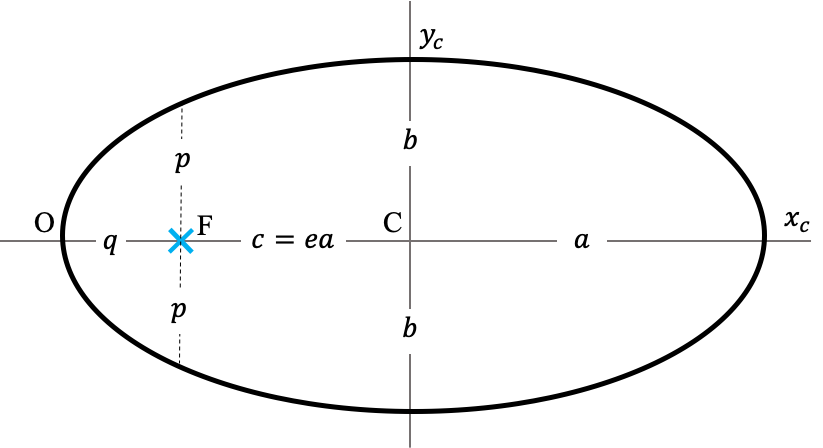
\includegraphics[width=0.6\textwidth]{./figures/horizontal_elipse.png}
\caption{Parámetros geométricos de la elipse referidos al apside O, el
foco F y el centro C: \(a\) semieje mayor, \(b\) semieje menor, \(p\)
\emph{semilatus rectum}, \(e\) excentricidad, \(c\) distancia
foco-centro.\label{fig:elipse}}
\end{figure}

Un resultado interesante, que podemos agregar a las definiciones
geométricas de Apolonio y Democrito, resulta al combinar la definición
de \(a\) con la distancia de un apside al foco más cercano \(q\). Es
claro de la \autoref{fig:elipse_hiperbola} que la distancia entre el
centro y el foco de la elipse, que llamaremos en lo sucesivo \(c\) es:

\begin{eqnarray}
\nonumber
c & = & a-q\\
 \nonumber
  & = & \frac{p}{1-e^2}-\frac{p}{1+e}\\
  \nonumber
\end{eqnarray} o en términos simples:

\begin{equation}
c = ae
\end{equation}

Este resultado se puede interpretar diciendo que la excentricidad de una
elipse \(e=c/a\) es el grado en el que el foco esta desplazado a partir
del centro geométrico de la figura y medido en unidades del semieje
mayor \(a\). De allí precisamente el nombre de este parámetro.

Uno podría entonces cuantificar la excentricidad de una elipse como un
porcentaje. Así por ejemplo, la órbita \emph{osculatriz} de Marte
(volveremos sobre este concepto en el
\autoref{problema_doscuerpos}), que fue el planeta utilizado por
Kepler para descubrir que las órbitas planetarias eran elipses, es una
elipse con una excentricidad de \(9.3\%\).

Es decir, el centro geométrico de la órbita de Marte esta desplazado
respecto a su foco (donde se ubica el Sol o más precisamente el centro
de masa del Sistema Solar) un \(9.3\%\) del eje mayor (la distancia
promedio de Marte al Sol.) Este desplazamiento (que es significativo)
fue la clave precisamente de porque fue más fácil para Kepler deducir la
elipticidad de la trayectoria de ese planeta, de lo que lo fue para
todos los astrónomos antes que él deducirlo usando la trayectoria de
todos los demás planetas (en comparación las excentricidades de las
órbitas osculatrices de la Tierra y de Júpiter, por ejemplo, son
\(1.6\%\) y \$4.8\%, respectivamente.)

Utilice el código interactivo que viene con las libretas en la
\hreffoot{http://seap-udea.org/MecanicaCeleste_Zuluaga}{versión electrónica
del libro} para visualizar la forma de las órbitas de los planetas
mencionados y ver realmente, que tan diferentes de una circunferencia
son.

\hypertarget{subsubsec_conicas_hiperbola}{%
\subsection{Parámetros de la
hipérbola}\label{subsubsec_conicas_hiperbola}}

La interpretación geométrica de \(a\) y \(b\) en el caso de la hipérbola
(\(e>1\)) es un poco más complicada (ver la \autoref{fig:hiperbola}).

Para empezar el valor del parámetro \(a=p/(1-e^2)\) es negativo. Esto
implica que el punto \(C\), que hace la ecuación de la hipérbola la más
sencilla posible, esta a la izquierda del apside, contrario a lo que
pasa con la elipse. Llamamos a C, no el centro de la hipérbola sino su
\emph{vértice}.

No debemos confundir sin embargo el eje \(y_c\) en la
\autoref{fig:hiperbola} con la directriz de la hipérbola (ver
\autoref{fig:conicas_directriz}) que en realidad esta situada a una
distancia \(\alpha=a(1-e)/e\) (ver Ec. \ref{eq:alpha}.) La directriz y
el eje \(y_c\) se aproximan una a otra cuando \(e\rightarrow \infty\).

\begin{figure}[t!]
\centering
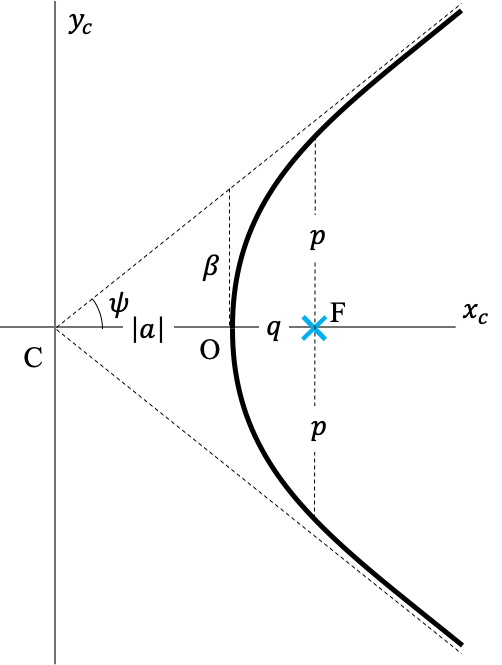
\includegraphics[width=0.6\textwidth]{./figures/vertical_hiperbola.png}
\caption{Parámetros geométricos de la hipérbola referidos al apside O,
el foco F y el vértice C: \(a\) distancia al vértice (llamado con
frecuencia también semieje mayor aunque en la hipérbola no hay tal),
\(\beta\) pendiente de la hipérbola, \(p\) \emph{semilatus rectum},
\(e\) excentricidad, \(\psi\) angulo de
semiapertura.\label{fig:elipse}}
\end{figure}

El parámetro \(b^2=a^2(1-e^2)\) es inconveniente dado que en este caso
\(e>1\) y por lo tanto \(b\) debería ser un número imaginario. Para
evitar este inconveniente reescribimos la ecuación de la hipérbola Ec.
(\ref{eq:ecuacion_centro}) como:

\begin{equation}
\label{eq:ecuacion_centro_hiperbola}
\frac{x_c^2}{a^2}-\frac{y_c^2}{\beta^2}=1
\end{equation} y definimos:

\begin{equation}
\label{eq:beta}
\beta\equiv |a|\sqrt{e^2-1}
\end{equation}

¿Cuál es la interpretación geométrica de \(\beta\)? Si despejamos
\(y_c\) de la Ec. (\ref{eq:ecuacion_centro_hiperbola}) tenemos:

\[
y_c=\pm\beta\sqrt{\frac{x_c^2}{a^2}-1}
\] donde los signos \(\pm\) corresponden a las ``ramas'' superior e
inferior de la hipérbola.

Aquí descubrimos una interesante propiedad de esta cónica: cuando
\(x_c\rightarrow \infty\), la hipérbola se aproxima a las recta:

\[
y_c\rightarrow\pm\frac{\beta}{|a|} x_c
\] que llamamos \emph{asíntotas}. La pendiente de las asíntotas,
\(\beta/|a|\) nos permite identificar a \(\beta\) como una cantidad que
cuántifica el grado de \emph{apertura} de la hipérbola respecto a su eje
de simetría: a mayor \(\beta\) (mayor excentricidad), mayor es la
pendiente de las asíntotas y más cerca esta la hipérbola de una línea
recta paralela a la directriz.

Otra manera de cuantificar la pendiente de las asintotas es usar el
ángulo \(\psi\):

\[
\tan\psi \equiv \frac{\beta}{|a|}
\]

No es difícil mostrar (ver problemas al final del capítulo), a partir de
la definición anterior, que:

\begin{equation}
\label{eq:cos_psi}
\cos\psi = \frac{1}{e}
\end{equation}

Para poner en un contexto astronómico este resultado, podemos mencionar
que en 2019 fue descubierto un cometa proveniente del espacio
interestelar, hoy conocido como el 2I/Borisov, cuya trayectoria respecto
al centro de masa del sistema solar es una hipérbola con \(e=3.35\).
Usando la Ec. (\ref{eq:cos_psi}) podemos calcular que las asíntotas de
su órbita se abren en un ángulo extremo de

    \begin{code}{}{}\begin{Verbatim}[fontsize=\small,commandchars=\\\{\}]
\PY{c+c1}{\PYZsh{}Cometa interestelar 2I/Borisov}
\PY{n}{e}\PY{o}{=}\PY{l+m+mf}{3.35}

\PY{k+kn}{from} \PY{n+nn}{numpy} \PY{k}{import} \PY{n}{arccos}
\PY{n}{psi}\PY{o}{=}\PY{n}{arccos}\PY{p}{(}\PY{l+m+mi}{1}\PY{o}{/}\PY{n}{e}\PY{p}{)}
\end{Verbatim}

%%

\end{code}
\vspace{-1em}

%%hidecode


    \begin{Verbatim}[fontsize=\small,commandchars=\\\{\}]
Psi = 72.63202008811639 grados
\end{Verbatim}

Utilice el código interactivo que viene con las libretas en la
\hreffoot{http://seap-udea.org/MecanicaCeleste_Zuluaga}{versión electrónica
del libro} para visualizar la forma de la órbita del 2I/Borisov.

\hypertarget{conicas_rotacion_plano}{%
\subsection{Rotación de las cónicas en el
plano}\label{conicas_rotacion_plano}}

Al comenzar la \autoref{conicas_algebraica}, habíamos mencionado dos
posibles transformaciones que nos conducían a la forma algebraica más
simple (la que obtuvimos en la \autoref{conicas_centro}) y a la más
general. La primera la obtuvimos simplemente aplicando una traslación de
los ejes coordenados:

\[
\begin{array}{rcl}
x_c &=& x_a-c\\
y_c &=& y_a
\end{array}
\]

Para obtener la forma más general, nos proponemos ahora realizar una
rotación.

Si llamamos \(x'\), \(y'\), \(z'\) a las coordenadas de un punto con
respecto a los ejes rotados, puede demostrarse (ver problemas al final
del capítulo) que estas se relacionan con las coordenadas del mismo
punto en el sistema alineado con la cónica (eje \(x\) en dirección del
eje de simetría) a través de:

\begin{equation}
\label{eq:rotacion2d}
\begin{array}{rcl}
x' & = & x \cos\theta + y \sin\theta \\
y' & = & - x \sin\theta + y \cos\theta \\
z' & = & z \\
\end{array}
\end{equation} donde \(\theta\) es el ángulo que forma el eje \(x'\) con
el eje \(x\) (ver \autoref{fig:rotacion}.)

Matricialmente estas relaciones se pueden escribir como:

\begin{equation}
\label{eq:rotacion2d_matricial}
\left(
\begin{array}{c}
x' \\
y' \\
z'
\end{array}
\right)
= R_z(\theta)
\left(
\begin{array}{c}
x \\
y \\
z
\end{array}
\right)
\end{equation} donde la matriz \(R_z(\theta)\) esta dada por:

\begin{equation}
\label{eq:matriz_rotacion2d}
R_z(\theta) =
\left(
\begin{array}{ccc}
\cos\theta & \sin\theta & 0 \\
-\sin\theta & \cos\theta & 0 \\
0 & 0 & 1 \\
\end{array}
\right)
\end{equation} y el subíndice \(z\) indica que la rotación se realiza
alrededor de este eje.

La matriz de rotación \(R_z(\theta)\) es una matriz \emph{unitaria} que
tiene las siguientes propiedades:

\begin{itemize}
\tightlist
\item
  Determinante, \(\det R_z=1\).
\item
  Inversa, \(R_z^{-1}=R_z^T\)
\end{itemize}

Esta última propiedad implica que:

\begin{equation}
\label{eq:inversa_matriz_rotacion}
R_z^{-1}(\theta)=R_z(-\theta)
\end{equation} que será muy conveniente para lo que viene.

Usando las propiedades de \(R_z\) podemos encontrar la transformación
inversa a la Ec. (\ref{eq:rotacion2d}):

\begin{equation}
\label{eq:rotacion2d_inversa_matricial}
\left(
\begin{array}{c}
x \\
y \\
z
\end{array}
\right)
= R_z(-\theta)
\left(
\begin{array}{c}
x' \\
y' \\
z'
\end{array}
\right)
\end{equation} o explícitamente:

\begin{equation}
\label{eq:rotacion2d_inversa}
\begin{array}{rcl}
x & = & x' \cos\theta - y' \sin\theta \\
x & = & x' \sin\theta + y' \cos\theta \\
z & = & z' \\
\end{array}
\end{equation}

El sistema \texttt{SPICE} contiene una rutina útil para definir de
manera sencilla una matriz de rotación dado un ángulo y un eje respecto
al que se realiza la rotación:

    \begin{code}{Algoritmo}{code:spice_rotate}\begin{Verbatim}[fontsize=\small,commandchars=\\\{\}]
\PY{k+kn}{from} \PY{n+nn}{spiceypy} \PY{k}{import} \PY{n}{rotate}
\PY{k+kn}{from} \PY{n+nn}{numpy} \PY{k}{import} \PY{n}{pi}
\PY{n}{Rz}\PY{o}{=}\PY{n}{rotate}\PY{p}{(}\PY{n}{pi}\PY{o}{/}\PY{l+m+mi}{6}\PY{p}{,}\PY{l+m+mi}{3}\PY{p}{)}
\end{Verbatim}

%%

\end{code}
\vspace{-1em}

%%hidecode


    \begin{Verbatim}[fontsize=\small,commandchars=\\\{\}]
Rz(30 grados) = 
[[ 0.8660254  0.5        0.       ]
 [-0.5        0.8660254  0.       ]
 [ 0.         0.         1.       ]]
\end{Verbatim}

Que coincide con la definición dada por la Ec.
(\ref{eq:matriz_rotacion2d}).

\hypertarget{conicas_ecuacion_general}{%
\subsection{Ecuación general de las
cónicas}\label{conicas_ecuacion_general}}

Qué pasa entonces si, partiendo de la ecuación general respecto al
apside (Ec. \ref{eq:ecuacion_apside_pe}) hacemos primero una traslación
a un punto con coordenadas \((t_x,t_y)\):

\[
(y+t_y)^2-2p(x+t_x)-(e^2-1)(x+t_x)^2=0
\] y una vez trasladados al nuevo origen, realizamos una rotación a unos
nuevos ejes \((x',y')\) realizando para ello la transformación dada por
las Ecs. (\ref{eq:rotacion2d_inversa}):

\[
[(x'\sin\theta + y'\cos\theta)+t_y]^2-2p [(x'\cos\theta - y'\sin\theta)+t_x] -(e^2-1) [(x'\cos\theta - y'\sin\theta)+t_x]^2 = 0
\]

Expandiendo y recogiendo términos comunes, la ecuación general de una
cónica trasladada y rotada será:

\begin{equation}
\label{eq:ecuacion_conica_trasladada_rotada}
\begin{array}{rcc}
x'^2 (1- e^2 \cos^2\theta)+x'y'(e^2 \sin2\theta)+y'^2 (1- e^2 \sin^2\theta) & + & \\
x' [2 t_y \sin\theta - 2 p \cos\theta + 2 t_x \cos\theta (1-e^2)] & + & \\ 
y' [2 t_y \cos\theta + 2 p \sin\theta - 2 t_x \sin\theta (1-e^2)] & + & \\
t_x^2 (1- e^2) - 2 p t_x + t_y^2 & = & 0
\end{array}
\end{equation} que puede escribirse de forma general, como:

\begin{equation}
\label{eq:ecuacion_general}
\displaystyle Ax'^2 + Bx'y' + Cy'^2 + Dx' + Ey' + F = 0
\end{equation} con:

\begin{equation}
\label{eq:ecuacion_general_coeficientes}
\begin{array}{rcl}
A &=&  1 - e^2 \cos^2\theta\\
B &=&  e^2 \sin2\theta\\
C &=&  1 - e^2 \sin^2\theta\\
D &=& 2 t_y \sin\theta - 2 p \cos\theta + 2 t_x \cos\theta (1-e^2)\\
E &=& 2 t_y \cos\theta + 2 p \sin\theta - 2 t_x \sin\theta (1-e^2)\\
F &=& t_x^2 (1- e^2) - 2 p t_x + t_y^2
\end{array}
\end{equation}

Es decir, cualquier curva en el plano cuyos puntos obedezcan una
ecuación cuadrática general de la forma Ec. (\ref{eq:ecuacion_general})
es una cónica con una orientación, tamaño, forma y posición de los
apsides que dependerá de los coeficientes \(A\), \(B\), \(C\), \(D\),
\(E\) y \(F\).

Dada la ecuación algebraica de una cónica, expresada en la forma
cuadrática general (Ec. \ref{eq:ecuacion_general}), es posible, usando
los coeficiende \(A\), \(B\) y \(C\) determinar qué tipo de cónica y su
orientación en el esepacio.

Para ello es posible, combinando algunas de las Ecs.
(\ref{:ecuacion_general_coeficientes}), demostrar que:

\begin{equation}
\label{eq:eta_ecuacion_general}
\eta=1-(A+C)
\end{equation} y por otro lado:

\begin{equation}
\label{eq:teta_ecuacion_general}
\tan 2\theta=\frac{B}{C-A}
\end{equation}

Si además se usan los valores de los coeficientes \(D\) y \(E\), es
posible determinar la ordenada del vértice de la cónica:

\begin{equation}
\label{eq:ty_ecuacion_general}
t_y=\frac{D\sin\theta+E\cos\theta}{2}
\end{equation}

Expresiones mucho más complejas pueden derivarse para \(t_x\) y para
\(p\) en función de los coeficientes \(D\), \(E\) y \(F\), que también
dependen de ellos (ver problemas al final del capítulo.) Sin embargo,
una vez el apside de la cónica ha sido localizada sobre el eje de las
abcisas (realizando la traslación inversa \(-t_y\)) y ha sido rotada en
un ángulo \(\theta\) dado por la Ec. (\ref{eq:teta_ecuacion_general})
para que su eje de simetría coincida con el eje \(x\), las demás
propiedades de la curva pueden obtenerse más fácilmente.

\hypertarget{grafico_conica_rotada_plano}{%
\subsection{Gráfico de una cónica rotada en el
plano}\label{grafico_conica_rotada_plano}}

Podemos poner en práctica algunos de los resultados de las secciones
anteriores (siempre es importante hacerlo para garantizar que todo se ha
entendido bien), construyendo numéricamente una cónica con la Ec.
(\ref{eq:ecuacion_apside_pe}) y aplicando traslaciones y rotaciones a la
misma para ver el efecto y escribir la ecuación general cuadrática (Ec.
\ref{eq:ecuacion_general}) que la describe.

Comencemos, escogiendo las propiedades de nuestra cónica y determinando,
el rango de valores de las coordenadas \(x_a\) de los puntos sobre la
cónica, en el sistema de coordenadas que tiene origen en el ápside:

    \begin{code}{}{}\begin{Verbatim}[fontsize=\small,commandchars=\\\{\}]
\PY{n}{p}\PY{o}{=}\PY{l+m+mf}{10.0}
\PY{n}{e}\PY{o}{=}\PY{l+m+mf}{0.8}

\PY{c+c1}{\PYZsh{}Parametro eta}
\PY{n}{eta}\PY{o}{=}\PY{n}{e}\PY{o}{*}\PY{o}{*}\PY{l+m+mi}{2}\PY{o}{\PYZhy{}}\PY{l+m+mi}{1}

\PY{c+c1}{\PYZsh{}Conjunto de valores de x de la cónica}
\PY{k+kn}{from} \PY{n+nn}{numpy} \PY{k}{import} \PY{n}{linspace}
\PY{k}{if} \PY{n}{e}\PY{o}{==}\PY{l+m+mi}{1}\PY{p}{:}
    \PY{n}{a}\PY{o}{=}\PY{n}{p}
\PY{k}{else}\PY{p}{:}
    \PY{n}{a}\PY{o}{=}\PY{n}{p}\PY{o}{/}\PY{p}{(}\PY{l+m+mi}{1}\PY{o}{\PYZhy{}}\PY{n}{e}\PY{o}{*}\PY{o}{*}\PY{l+m+mi}{2}\PY{p}{)}

\PY{c+c1}{\PYZsh{}Rango de valores de x}
\PY{n}{xs}\PY{o}{=}\PY{n}{linspace}\PY{p}{(}\PY{l+m+mi}{0}\PY{p}{,}\PY{l+m+mi}{2}\PY{o}{*}\PY{n+nb}{abs}\PY{p}{(}\PY{n}{a}\PY{p}{)}\PY{p}{,}\PY{l+m+mi}{100}\PY{p}{)}
\end{Verbatim}

%%

\end{code}

Nótese que \(a\) no esta definido en el caso de una parábola \(e=1\)
(para una elipse y una hipérbola \(a=p/(1-e^2)\), ver Ec.
\ref{eq:semiejemayor}.) Por esa razón en el algoritmo anterior hemos
escogido definir \(a\equiv p\) cuando \(e=1\), únicamente con el
propósito de usar una sola expresión
\texttt{xs=linspace(0,2*abs(a),100)} para calcular el rango de valores
de las abcisas de la cónica.

Si bien sabemos que en el caso de parábolas e hipérbolas, los valores de
las abcisas son \(x_a\in [0,\infty)\) (ver
\autoref{fig:conicas_apolonio}), para una elipse es claro que
\(x_a\in [0,2a]\) (ver \autoref{fig:elipse}.)

Con los valores de \(x\) podemos ahora usar la Ec.
(\ref{eq:ecuacion_apside_pe}) para calcular los valores de la ordenada,
tanto para la rama superior de la cónica (por encima del eje de
simetría) como para la inferior:

    \begin{code}{}{}\begin{Verbatim}[fontsize=\small,commandchars=\\\{\}]
\PY{c+c1}{\PYZsh{}Ecuación de la cónica}
\PY{k+kn}{from} \PY{n+nn}{numpy} \PY{k}{import} \PY{n}{sqrt}
\PY{n}{ys\PYZus{}sup}\PY{o}{=}\PY{n}{sqrt}\PY{p}{(}\PY{l+m+mi}{2}\PY{o}{*}\PY{n}{p}\PY{o}{*}\PY{n}{xs}\PY{o}{+}\PY{n}{eta}\PY{o}{*}\PY{n}{xs}\PY{o}{*}\PY{o}{*}\PY{l+m+mi}{2}\PY{p}{)}
\PY{n}{ys\PYZus{}inf}\PY{o}{=}\PY{o}{\PYZhy{}}\PY{n}{sqrt}\PY{p}{(}\PY{l+m+mi}{2}\PY{o}{*}\PY{n}{p}\PY{o}{*}\PY{n}{xs}\PY{o}{+}\PY{n}{eta}\PY{o}{*}\PY{n}{xs}\PY{o}{*}\PY{o}{*}\PY{l+m+mi}{2}\PY{p}{)}
\end{Verbatim}

%%

\end{code}

Para los propósito de graficar la cónica, debemos duplicar los valores
de la lista \texttt{xs}. Sin embargo, y por razones que veremos abajo,
lo haremos ordenando de forma especial las coordenadas de los puntos,
comenzando primero con el punto más lejano al origen (\(x=2a\) o
\texttt{xs{[}-1{]},ys{[}-1{]}}), llegando hasta el origen mismo
\texttt{xs{[}0{]},ys{[}0{]}} y de allí regresando de nuevo al punto más
lejano.

En Python esta ``compleja'' operación puede abreviarse usando la
sintaxis genera para extraer tajadas de los arreglos:

    \begin{code}{}{}\begin{Verbatim}[fontsize=\small,commandchars=\\\{\}]
\PY{k+kn}{from} \PY{n+nn}{numpy} \PY{k}{import} \PY{n}{append}\PY{p}{,}\PY{n}{zeros\PYZus{}like}
\PY{n}{xs}\PY{o}{=}\PY{n}{append}\PY{p}{(}\PY{n}{xs}\PY{p}{[}\PY{p}{:}\PY{p}{:}\PY{o}{\PYZhy{}}\PY{l+m+mi}{1}\PY{p}{]}\PY{p}{,}\PY{n}{xs}\PY{p}{)}
\PY{n}{ys}\PY{o}{=}\PY{n}{append}\PY{p}{(}\PY{n}{ys\PYZus{}sup}\PY{p}{[}\PY{p}{:}\PY{p}{:}\PY{o}{\PYZhy{}}\PY{l+m+mi}{1}\PY{p}{]}\PY{p}{,}\PY{n}{ys\PYZus{}inf}\PY{p}{)}
\PY{n}{zs}\PY{o}{=}\PY{n}{zeros\PYZus{}like}\PY{p}{(}\PY{n}{xs}\PY{p}{)}
\end{Verbatim}

%%

\end{code}

Un gráfico de los puntos de la cónica en el sistema de referencia del
ápside srá:

    \begin{code}{Algoritmo}{code:4_Fundamentos_7}\begin{Verbatim}[fontsize=\small,commandchars=\\\{\}]
\PY{k+kn}{import} \PY{n+nn}{matplotlib}\PY{n+nn}{.}\PY{n+nn}{pyplot} \PY{k}{as} \PY{n+nn}{plt}
\PY{n}{fig}\PY{o}{=}\PY{n}{plt}\PY{o}{.}\PY{n}{figure}\PY{p}{(}\PY{p}{)}
\PY{n}{ax}\PY{o}{=}\PY{n}{fig}\PY{o}{.}\PY{n}{gca}\PY{p}{(}\PY{p}{)}

\PY{n}{ax}\PY{o}{.}\PY{n}{plot}\PY{p}{(}\PY{n}{xs}\PY{p}{,}\PY{n}{ys}\PY{p}{,}\PY{l+s+s1}{\PYZsq{}}\PY{l+s+s1}{b\PYZhy{}}\PY{l+s+s1}{\PYZsq{}}\PY{p}{)}

\PY{k+kn}{from} \PY{n+nn}{pymcel}\PY{n+nn}{.}\PY{n+nn}{plot} \PY{k}{import} \PY{n}{fija\PYZus{}ejes\PYZus{}proporcionales}
\PY{n}{valores}\PY{o}{=}\PY{p}{(}\PY{n}{xs}\PY{p}{,}\PY{n}{ys}\PY{p}{)}
\PY{n}{fija\PYZus{}ejes\PYZus{}proporcionales}\PY{p}{(}\PY{n}{ax}\PY{p}{,}\PY{n}{valores}\PY{p}{,}\PY{n}{xmin}\PY{o}{=}\PY{l+m+mi}{0}\PY{p}{,}\PY{n}{ycm}\PY{o}{=}\PY{l+m+mi}{0}\PY{p}{)}\PY{p}{;}
\PY{n}{ax}\PY{o}{.}\PY{n}{grid}\PY{p}{(}\PY{p}{)}
\end{Verbatim}

%%

\tcblower
\footnotesize
\em ver Figura \ref{fig:code:4_Fundamentos_7}
\end{code}

    \begin{center}

\begin{figure}[ht!]
\centering
    \adjustimage{max size={0.8\linewidth}{0.8\paperheight}}{combined_files/combined_341_0.png}
\caption{Figura correspondiente al código \ref{code:4_Fundamentos_7}.\label{fig:code:4_Fundamentos_7}}
\end{figure}

    \end{center}
%{ \hspace*{\fill} \\}
    
Ahora podemos trasladar la cónica:

    \begin{code}{}{}\begin{Verbatim}[fontsize=\small,commandchars=\\\{\}]
\PY{c+c1}{\PYZsh{}Parámetros de la traslación}
\PY{n}{tx}\PY{o}{=}\PY{l+m+mf}{15.0}
\PY{n}{ty}\PY{o}{=}\PY{o}{\PYZhy{}}\PY{l+m+mf}{10.0}

\PY{c+c1}{\PYZsh{}Coordenadas trasladadas}
\PY{n}{xs}\PY{o}{=}\PY{n}{xs}\PY{o}{\PYZhy{}}\PY{n}{tx}
\PY{n}{ys}\PY{o}{=}\PY{n}{ys}\PY{o}{\PYZhy{}}\PY{n}{ty}
\end{Verbatim}

%%

\end{code}

Construimos la matriz de rotación usando las rutinas de \texttt{SPICE}
(ver Alg. \ref{code:spice_rotate}):

    \begin{code}{}{}\begin{Verbatim}[fontsize=\small,commandchars=\\\{\}]
\PY{k+kn}{from} \PY{n+nn}{spiceypy} \PY{k}{import} \PY{n}{rotate}
\PY{k+kn}{from} \PY{n+nn}{numpy} \PY{k}{import} \PY{n}{pi}
\PY{n}{teta}\PY{o}{=}\PY{n}{pi}\PY{o}{/}\PY{l+m+mi}{6}
\PY{n}{Rz}\PY{o}{=}\PY{n}{rotate}\PY{p}{(}\PY{n}{teta}\PY{p}{,}\PY{l+m+mi}{3}\PY{p}{)}
\end{Verbatim}

%%

\end{code}

La rotación de los puntos de la cónica contenidos en las listas
\texttt{xs}, \texttt{ys} usando la Ec. (\ref{eq:rotacion2d_matricial}),
no es tan trivial en \texttt{Python}. Para ello definiremos una rutina
general que usaremos más adelante en el libro:

    \begin{code}{Algoritmo}{code:rota_puntos}\begin{Verbatim}[fontsize=\small,commandchars=\\\{\}]
\PY{k}{def} \PY{n+nf}{rota\PYZus{}puntos}\PY{p}{(}\PY{n}{R}\PY{p}{,}\PY{n}{x}\PY{p}{,}\PY{n}{y}\PY{p}{,}\PY{n}{z}\PY{p}{)}\PY{p}{:}
    \PY{k+kn}{from} \PY{n+nn}{spiceypy} \PY{k}{import} \PY{n}{mxv}
    \PY{k+kn}{from} \PY{n+nn}{numpy} \PY{k}{import} \PY{n}{zeros\PYZus{}like}
    \PY{n}{N}\PY{o}{=}\PY{n+nb}{len}\PY{p}{(}\PY{n}{x}\PY{p}{)}
    \PY{n}{xp}\PY{o}{=}\PY{n}{zeros\PYZus{}like}\PY{p}{(}\PY{n}{x}\PY{p}{)}
    \PY{n}{yp}\PY{o}{=}\PY{n}{zeros\PYZus{}like}\PY{p}{(}\PY{n}{y}\PY{p}{)}
    \PY{n}{zp}\PY{o}{=}\PY{n}{zeros\PYZus{}like}\PY{p}{(}\PY{n}{z}\PY{p}{)}
    \PY{k}{for} \PY{n}{i} \PY{o+ow}{in} \PY{n+nb}{range}\PY{p}{(}\PY{n}{N}\PY{p}{)}\PY{p}{:}
        \PY{n}{xp}\PY{p}{[}\PY{n}{i}\PY{p}{]}\PY{p}{,}\PY{n}{yp}\PY{p}{[}\PY{n}{i}\PY{p}{]}\PY{p}{,}\PY{n}{zp}\PY{p}{[}\PY{n}{i}\PY{p}{]}\PY{o}{=}\PY{n}{mxv}\PY{p}{(}\PY{n}{R}\PY{p}{,}\PY{p}{[}\PY{n}{x}\PY{p}{[}\PY{n}{i}\PY{p}{]}\PY{p}{,}\PY{n}{y}\PY{p}{[}\PY{n}{i}\PY{p}{]}\PY{p}{,}\PY{n}{z}\PY{p}{[}\PY{n}{i}\PY{p}{]}\PY{p}{]}\PY{p}{)}
    \PY{k}{return} \PY{n}{xp}\PY{p}{,}\PY{n}{yp}\PY{p}{,}\PY{n}{zp}
\end{Verbatim}

%%

\end{code}

Los puntos rotados de la cónica serán:

    \begin{code}{}{}\begin{Verbatim}[fontsize=\small,commandchars=\\\{\}]
\PY{n}{xps}\PY{p}{,}\PY{n}{yps}\PY{p}{,}\PY{n}{zps}\PY{o}{=}\PY{n}{rota\PYZus{}puntos}\PY{p}{(}\PY{n}{Rz}\PY{p}{,}\PY{n}{xs}\PY{p}{,}\PY{n}{ys}\PY{p}{,}\PY{n}{zs}\PY{p}{)}
\end{Verbatim}

%%

\end{code}

Y una gráfica de los puntos rotados:

    \begin{code}{Algoritmo}{code:4_Fundamentos_8}\begin{Verbatim}[fontsize=\small,commandchars=\\\{\}]
\PY{k+kn}{import} \PY{n+nn}{matplotlib}\PY{n+nn}{.}\PY{n+nn}{pyplot} \PY{k}{as} \PY{n+nn}{plt}
\PY{n}{fig}\PY{o}{=}\PY{n}{plt}\PY{o}{.}\PY{n}{figure}\PY{p}{(}\PY{p}{)}
\PY{n}{ax}\PY{o}{=}\PY{n}{fig}\PY{o}{.}\PY{n}{gca}\PY{p}{(}\PY{p}{)}

\PY{n}{ax}\PY{o}{.}\PY{n}{plot}\PY{p}{(}\PY{n}{xps}\PY{p}{,}\PY{n}{yps}\PY{p}{,}\PY{l+s+s1}{\PYZsq{}}\PY{l+s+s1}{b\PYZhy{}}\PY{l+s+s1}{\PYZsq{}}\PY{p}{)}

\PY{k+kn}{from} \PY{n+nn}{pymcel}\PY{n+nn}{.}\PY{n+nn}{plot} \PY{k}{import} \PY{n}{fija\PYZus{}ejes\PYZus{}proporcionales}
\PY{n}{valores}\PY{o}{=}\PY{p}{(}\PY{n}{xps}\PY{p}{,}\PY{n}{yps}\PY{p}{)}
\PY{n}{fija\PYZus{}ejes\PYZus{}proporcionales}\PY{p}{(}\PY{n}{ax}\PY{p}{,}\PY{n}{valores}\PY{p}{)}\PY{p}{;}
\PY{n}{ax}\PY{o}{.}\PY{n}{grid}\PY{p}{(}\PY{p}{)}
\end{Verbatim}

%%

\tcblower
\footnotesize
\em ver Figura \ref{fig:code:4_Fundamentos_8}
\end{code}

    \begin{center}

\begin{figure}[ht!]
\centering
    \adjustimage{max size={0.8\linewidth}{0.8\paperheight}}{combined_files/combined_351_0.png}
\caption{Figura correspondiente al código \ref{code:4_Fundamentos_8}.\label{fig:code:4_Fundamentos_8}}
\end{figure}

    \end{center}
%{ \hspace*{\fill} \\}
    
Los valores de los coeficientes del polinomio de segundo grado
\(P(x,y)=Ax^2+By^2+Cxy+Dx+Ey+F\) que describe los puntos del gráfico
anterior, son (Ec. \ref{eq:ecuacion_general_coeficientes}):

    \begin{code}{}{}\begin{Verbatim}[fontsize=\small,commandchars=\\\{\}]
\PY{k+kn}{from} \PY{n+nn}{numpy} \PY{k}{import} \PY{n}{sin}\PY{p}{,}\PY{n}{cos}
\PY{n}{A}\PY{o}{=}\PY{l+m+mi}{1}\PY{o}{\PYZhy{}}\PY{n}{e}\PY{o}{*}\PY{o}{*}\PY{l+m+mi}{2}\PY{o}{*}\PY{n}{cos}\PY{p}{(}\PY{n}{teta}\PY{p}{)}\PY{o}{*}\PY{o}{*}\PY{l+m+mi}{2}
\PY{n}{B}\PY{o}{=}\PY{n}{e}\PY{o}{*}\PY{o}{*}\PY{l+m+mi}{2}\PY{o}{*}\PY{n}{sin}\PY{p}{(}\PY{l+m+mi}{2}\PY{o}{*}\PY{n}{teta}\PY{p}{)}
\PY{n}{C}\PY{o}{=}\PY{l+m+mi}{1}\PY{o}{\PYZhy{}}\PY{n}{e}\PY{o}{*}\PY{o}{*}\PY{l+m+mi}{2}\PY{o}{*}\PY{n}{sin}\PY{p}{(}\PY{n}{teta}\PY{p}{)}\PY{o}{*}\PY{o}{*}\PY{l+m+mi}{2}
\PY{n}{D}\PY{o}{=}\PY{l+m+mi}{2}\PY{o}{*}\PY{n}{ty}\PY{o}{*}\PY{n}{sin}\PY{p}{(}\PY{n}{teta}\PY{p}{)}\PY{o}{\PYZhy{}}\PY{l+m+mi}{2}\PY{o}{*}\PY{n}{p}\PY{o}{*}\PY{n}{cos}\PY{p}{(}\PY{n}{teta}\PY{p}{)}\PY{o}{+}\PY{l+m+mi}{2}\PY{o}{*}\PY{n}{tx}\PY{o}{*}\PY{n}{cos}\PY{p}{(}\PY{n}{teta}\PY{p}{)}\PY{o}{*}\PY{p}{(}\PY{l+m+mi}{1}\PY{o}{\PYZhy{}}\PY{n}{e}\PY{o}{*}\PY{o}{*}\PY{l+m+mi}{2}\PY{p}{)}
\PY{n}{E}\PY{o}{=}\PY{l+m+mi}{2}\PY{o}{*}\PY{n}{ty}\PY{o}{*}\PY{n}{cos}\PY{p}{(}\PY{n}{teta}\PY{p}{)}\PY{o}{+}\PY{l+m+mi}{2}\PY{o}{*}\PY{n}{p}\PY{o}{*}\PY{n}{sin}\PY{p}{(}\PY{n}{teta}\PY{p}{)}\PY{o}{\PYZhy{}}\PY{l+m+mi}{2}\PY{o}{*}\PY{n}{tx}\PY{o}{*}\PY{n}{sin}\PY{p}{(}\PY{n}{teta}\PY{p}{)}\PY{o}{*}\PY{p}{(}\PY{l+m+mi}{1}\PY{o}{\PYZhy{}}\PY{n}{e}\PY{o}{*}\PY{o}{*}\PY{l+m+mi}{2}\PY{p}{)}
\PY{n}{F}\PY{o}{=}\PY{n}{tx}\PY{o}{*}\PY{o}{*}\PY{l+m+mi}{2}\PY{o}{*}\PY{p}{(}\PY{l+m+mi}{1}\PY{o}{\PYZhy{}}\PY{n}{e}\PY{o}{*}\PY{o}{*}\PY{l+m+mi}{2}\PY{p}{)}\PY{o}{\PYZhy{}}\PY{l+m+mi}{2}\PY{o}{*}\PY{n}{p}\PY{o}{*}\PY{n}{tx}\PY{o}{+}\PY{n}{ty}\PY{o}{*}\PY{o}{*}\PY{l+m+mi}{2}
\end{Verbatim}

%%

\end{code}
\vspace{-1em}

%%hidecode


    \begin{Verbatim}[fontsize=\small,commandchars=\\\{\}]
A = 0.5199999999999998
B = 0.5542562584220408
C = 0.84
D = -17.967433714816835
E = -12.720508075688773
F = -119.00000000000003
Ecuación: (0.52)x\^{}2+(0.55)xy+(0.84)y\^{}2+(-18)x+(-13)y+(-119.0)=0
\end{Verbatim}

Podemos ahora verificar la afirmación que los puntos de la cónica
satisfacen la ecuación \(P(x,y)=0\) (Ec. \ref{eq:ecuacion_general}),
construyendo primero una rutina para calcular, dado cualquier punto
\((x,y)\) el valor del polinomio \(P(x,y)\):

    \begin{code}{Algoritmo}{code:polinomio_segundo_grado}\begin{Verbatim}[fontsize=\small,commandchars=\\\{\}]
\PY{k}{def} \PY{n+nf}{polinomio\PYZus{}segundo\PYZus{}grado}\PY{p}{(}\PY{n}{coeficientes}\PY{p}{,}\PY{n}{x}\PY{p}{,}\PY{n}{y}\PY{p}{)}\PY{p}{:}
    \PY{n}{A}\PY{p}{,}\PY{n}{B}\PY{p}{,}\PY{n}{C}\PY{p}{,}\PY{n}{D}\PY{p}{,}\PY{n}{E}\PY{p}{,}\PY{n}{F}\PY{o}{=}\PY{n}{coeficientes}
    \PY{n}{P}\PY{o}{=}\PY{n}{A}\PY{o}{*}\PY{n}{x}\PY{o}{*}\PY{o}{*}\PY{l+m+mi}{2}\PY{o}{+}\PY{n}{B}\PY{o}{*}\PY{n}{x}\PY{o}{*}\PY{n}{y}\PY{o}{+}\PY{n}{C}\PY{o}{*}\PY{n}{y}\PY{o}{*}\PY{o}{*}\PY{l+m+mi}{2}\PY{o}{+}\PY{n}{D}\PY{o}{*}\PY{n}{x}\PY{o}{+}\PY{n}{E}\PY{o}{*}\PY{n}{y}\PY{o}{+}\PY{n}{F}
    \PY{k}{return} \PY{n}{P}
\end{Verbatim}

%%

\end{code}

Si calculamos el valor de \(P(x,y)\) para todos los puntos \texttt{xps}
y \texttt{yps} verificamos la afirmación:

    \begin{code}{}{}\begin{Verbatim}[fontsize=\small,commandchars=\\\{\}]
\PY{n}{coeficientes}\PY{o}{=}\PY{n}{A}\PY{p}{,}\PY{n}{B}\PY{p}{,}\PY{n}{C}\PY{p}{,}\PY{n}{D}\PY{p}{,}\PY{n}{E}\PY{p}{,}\PY{n}{F}
\PY{n}{Pxpsyps}\PY{o}{=}\PY{n}{polinomio\PYZus{}segundo\PYZus{}grado}\PY{p}{(}\PY{n}{coeficientes}\PY{p}{,}\PY{n}{xps}\PY{p}{,}\PY{n}{yps}\PY{p}{)}
\end{Verbatim}

%%

\end{code}

    \begin{code}{}{}\begin{Verbatim}[fontsize=\small,commandchars=\\\{\}]
\PY{n+nb}{print}\PY{p}{(}\PY{n}{f}\PY{l+s+s2}{\PYZdq{}}\PY{l+s+s2}{P(xps,yps):}\PY{l+s+se}{\PYZbs{}n}\PY{l+s+si}{\PYZob{}Pxpsyps[:5]\PYZcb{}}\PY{l+s+s2}{...}\PY{l+s+s2}{\PYZdq{}}\PY{p}{)}
\end{Verbatim}

%%

\end{code}

    \begin{Verbatim}[fontsize=\small,commandchars=\\\{\}]
P(xps,yps):
[ 2.84217094e-14 -1.13686838e-13 -1.13686838e-13 -7.10542736e-14
 -5.68434189e-14]{\ldots}
\end{Verbatim}

O para verificarlo en todos los puntos, podemos sumar el valor absoluto
de los valores de \texttt{Pxpsyps}:

    \begin{code}{}{}\begin{Verbatim}[fontsize=\small,commandchars=\\\{\}]
\PY{n}{Psum}\PY{o}{=}\PY{n+nb}{sum}\PY{p}{(}\PY{n+nb}{abs}\PY{p}{(}\PY{n}{Pxpsyps}\PY{p}{)}\PY{p}{)}
\end{Verbatim}

%%

\end{code}
\vspace{-1em}

%%hidecode


    \begin{Verbatim}[fontsize=\small,commandchars=\\\{\}]
Sum |P(xps,yps)| = 1.1738165994756855e-11
\end{Verbatim}

Finalmente podemos poner a prueba las Ecs.
(\ref{eq:eq:eta_ecuacion_general}), (\ref{eq:teta_ecuacion_general}) y
(\ref{eq:ty_ecuacion_general}):

    \begin{code}{}{}\begin{Verbatim}[fontsize=\small,commandchars=\\\{\}]
\PY{c+c1}{\PYZsh{}Parámetro de forma}
\PY{n}{eta\PYZus{}num}\PY{o}{=}\PY{l+m+mi}{1}\PY{o}{\PYZhy{}}\PY{p}{(}\PY{n}{A}\PY{o}{+}\PY{n}{C}\PY{p}{)}

\PY{c+c1}{\PYZsh{}Ángulo}
\PY{k+kn}{from} \PY{n+nn}{numpy} \PY{k}{import} \PY{n}{arctan}\PY{p}{,}\PY{n}{sin}\PY{p}{,}\PY{n}{cos}
\PY{n}{teta\PYZus{}num}\PY{o}{=}\PY{l+m+mf}{0.5}\PY{o}{*}\PY{n}{arctan}\PY{p}{(}\PY{n}{B}\PY{o}{/}\PY{p}{(}\PY{n}{C}\PY{o}{\PYZhy{}}\PY{n}{A}\PY{p}{)}\PY{p}{)}

\PY{c+c1}{\PYZsh{}Desplazamiento vertical}
\PY{n}{ty\PYZus{}num}\PY{o}{=}\PY{p}{(}\PY{n}{D}\PY{o}{*}\PY{n}{sin}\PY{p}{(}\PY{n}{teta\PYZus{}num}\PY{p}{)}\PY{o}{+}\PY{n}{E}\PY{o}{*}\PY{n}{cos}\PY{p}{(}\PY{n}{teta\PYZus{}num}\PY{p}{)}\PY{p}{)}\PY{o}{/}\PY{l+m+mi}{2}
\end{Verbatim}

%%

\end{code}
\vspace{-1em}

%%hidecode


    \begin{Verbatim}[fontsize=\small,commandchars=\\\{\}]
eta original = -0.36, eta numérico = -0.36
teta original = 30, teta numérico = 30
ty original = -10, ty numérico = -10
\end{Verbatim}

Como era de esperarse, la coincidencia es perfecta.

\hypertarget{conicas_sintesis_algebraica}{%
\subsection{Síntesis algebraica}\label{conicas_sintesis_algebraica}}

En la \autoref{conicas_nombre_algebra} mostramos como las
definiciones abstractas de la antigüedad, basadas en áreas y
proporciones, se convirtieron en la edad baja edad media y el
renacimiento, en ecuaciones algebraicas. Las representaciones
algebraicas permiten describir de forma sintética y poderosa el lugar
geométrico de las cónicas.

En las secciones precedentes hemos visto como la descripción algebraica
de las cónicas depende de donde coloquemos el origen o en que dirección
escojamos los ejes del sistema de coordenadas. De acuerdo a estas
elecciones reconocimos hasta ahora 4 formas distintas de describir
algebraicamente cualquier cónica, una vez especificados un parámetro de
tamaño, por ejemplo el \emph{semilatus rectum} \(p\) y uno de forma, por
ejemplo la excentricidad \(e\):

\begin{itemize}
\tightlist
\item
  Ecuación respecto al apside (origen en el ápside, eje \(x\) sobre el
  eje de simetría, Ec. \ref{eq:ecuacion_apside}): \[
  y_a^2-2p x_a -(e^2-1) x_a^2 = 0
  \]
\end{itemize}

\begin{itemize}
\item
  Ecuación respecto a la directriz (origen en la directriz, eje \(x\)
  sobre el eje de simetría, Ec. \ref{eq:directriz}):

  \[
  y_d^2 - 2pe x_d -(e^2-1) x_d^2 + e^2p^2=0
  \]
\end{itemize}

\begin{itemize}
\item
  Ecuación respecto al centro (origen en el centro de simetría, eje
  \(x\) sobre el eje de simetría, Ec. \ref{eq:ecuacion_centro}, solo
  valida para \(e\neq 1\)):

  \[
  \frac{x_c^2}{a^2}\pm\frac{y_c^2}{b^2}=1
  \]

  donde \(a^2=p/(1-e^2)\), el signo ``\(+\)'' es para elipses (\(e<1\))
  en cuyo caso \(b^2=a^2(1-e^2)\) y el signo ``\(-\)'' es para hipérbola
  (\(e>1\)) para el cuál \(b^2=\beta^2=a^2(e^2-1)\).
\end{itemize}

\begin{itemize}
\item
  Ecuación general (origen en \(t_x,t_y\) y eje \(x'\) rotado un ángulo
  \(\theta\) respecto al eje de simetría, Ec.
  \ref{eq:ecuacion_general}):

  \[
  Ax'^2 + Bx'y' + Cy'^2 + Dx' + Ey' + F = 0
  \] con:

  \[
    \begin{array}{rcl}
    A &=&  1 - e^2 \cos^2\theta\\
    B &=&  e^2 \sin2\theta\\
    C &=&  1 - e^2 \sin^2\theta\\
    D &=& 2 t_y \sin\theta - 2 p \cos\theta + 2 t_x \cos\theta (1-e^2)\\
    E &=& 2 t_y \cos\theta + 2 p \sin\theta - 2 t_x \sin\theta (1-e^2)\\
    F &=& t_x^2 (1- e^2) - 2 p t_x + t_y^2.
    \end{array}
    \]
\end{itemize}



\hypertarget{conicas_cilindricas}{%
\subsection{Cónicas en coordenadas
cilíndricas}\label{conicas_cilindricas}}

Nos proponemos ahora a escribir la ecuación de la cónica, en coordenadas
cilíndricas con origen en uno de los focos. La ecuación resultante y los
resultados geométricos que se derivan de ella, es de primera importancia
para la mecánica celeste.

\begin{figure}[ht!]
\centering
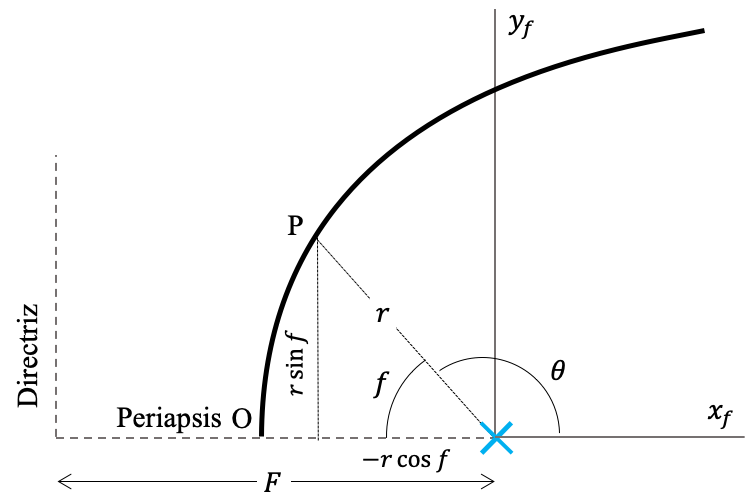
\includegraphics[width=0.5\textwidth]{./figures/horizontal_conica_foco.png}
\caption{Derivación de la ecuación de la cónica en coordenadas
cilíndricas referidas al Foco. En la figura el ángulo \(f\) es la
\emph{anomalía verdadera}.\label{fig:conica_foco}}
\end{figure}

Comenzando con la ecuación de la cónica referida a la directriz (Ec.
\ref{eq:ecuacion_directriz}) podemos aplicar una traslación al foco
haciendo \(x_d=x_f+F\) y \(y_d=y_f\):

\begin{equation}
\label{eq:ecuacion_foco}
y_f^2-(e^2-1)(x_f+F)^2-2F(x_f+F)+F^2=0
\end{equation}

Si escribribimos \(x_f,y_f\) en coordenadas cilíndricas como (ver Ecs.
\ref{eq:cilindricas_a_cartesianas}):

\begin{equation}
\label{eq:conica_parametricas_f}
\begin{array}{rcl}
x_f & = & -r \cos f\\
y_f & = & r \sin f\\
\end{array}
\end{equation} donde \(f\), en lugar de la coordenada cilíndrica
acimutal convencional \(\theta\) (que es un ángulo referido al semi eje
\(x+\)) el ángulo entre la dirección del periapsis y el radio vector del
punto (ver \autoref{fig:conica_foco_cilindiricas}), la Ec.
(\ref{eq:ecuacion_foco}), después de algunas manipulaciones algebraicas
se convierte en:

\begin{equation}
\label{eq:conica_ecuacion_cilindricas}
r = \frac{p}{1+e\cos f}
\end{equation} que es la ecuación fundamental de la cónica y que veremos
aparecer con mucha frecuencia en la mecánica celeste.

Las ecuaciones (\ref{eq:conica_parametricas}) y
(\ref{eq:conica_ecuacion_cilindricas}) evidencian un hecho interesante:
el ángulo \(f\) se puede usar para describir matemáticamente, usando un
sólo parámetro, las coordenadas cartesianas de los puntos sobre la
cónica. Esto hace mucho más sencillo encontrar la posición de los puntos
sobre estas curvas, en comparación como lo teníamos que hacer al usar
las ecuaciones algebraicas en \(x,y\) de las secciones anteriores.

Para ilustrar el poder de este resultado considere el siguiente
algoritmo para graficar una elipse y compárelo con el visto en la
\autoref{conica_ejercicio_numerico}:
%%HIDE%%
    \begin{code}{Algoritmo}{code:conica_dibujo}\begin{Verbatim}[fontsize=\small,commandchars=\\\{\}]
\PY{c+c1}{\PYZsh{}Parámetros}
\PY{n}{p}\PY{o}{=}\PY{l+m+mf}{10.0}
\PY{n}{e}\PY{o}{=}\PY{l+m+mf}{0.8}

\PY{c+c1}{\PYZsh{}Valores del ángulo}
\PY{k+kn}{from} \PY{n+nn}{numpy} \PY{k}{import} \PY{n}{linspace}\PY{p}{,}\PY{n}{pi}
\PY{n}{fs}\PY{o}{=}\PY{n}{linspace}\PY{p}{(}\PY{l+m+mi}{0}\PY{p}{,}\PY{l+m+mi}{2}\PY{o}{*}\PY{n}{pi}\PY{p}{,}\PY{l+m+mi}{100}\PY{p}{)}

\PY{c+c1}{\PYZsh{}Distancias }
\PY{k+kn}{from} \PY{n+nn}{numpy} \PY{k}{import} \PY{n}{cos}
\PY{n}{rs}\PY{o}{=}\PY{n}{p}\PY{o}{/}\PY{p}{(}\PY{l+m+mi}{1}\PY{o}{+}\PY{n}{e}\PY{o}{*}\PY{n}{cos}\PY{p}{(}\PY{n}{fs}\PY{p}{)}\PY{p}{)}

\PY{c+c1}{\PYZsh{}Coordenadas}
\PY{k+kn}{from} \PY{n+nn}{numpy} \PY{k}{import} \PY{n}{sin}
\PY{n}{xs}\PY{o}{=}\PY{n}{rs}\PY{o}{*}\PY{n}{cos}\PY{p}{(}\PY{n}{fs}\PY{p}{)}
\PY{n}{ys}\PY{o}{=}\PY{n}{rs}\PY{o}{*}\PY{n}{sin}\PY{p}{(}\PY{n}{fs}\PY{p}{)}

\PY{c+c1}{\PYZsh{}Gráfica}
\PY{k+kn}{import} \PY{n+nn}{matplotlib}\PY{n+nn}{.}\PY{n+nn}{pyplot} \PY{k}{as} \PY{n+nn}{plt}
\PY{n}{fig}\PY{o}{=}\PY{n}{plt}\PY{o}{.}\PY{n}{figure}\PY{p}{(}\PY{p}{)}
\PY{n}{ax}\PY{o}{=}\PY{n}{fig}\PY{o}{.}\PY{n}{gca}\PY{p}{(}\PY{p}{)}

\PY{c+c1}{\PYZsh{}Puntos cónica}
\PY{n}{ax}\PY{o}{.}\PY{n}{plot}\PY{p}{(}\PY{n}{xs}\PY{p}{,}\PY{n}{ys}\PY{p}{,}\PY{l+s+s1}{\PYZsq{}}\PY{l+s+s1}{b\PYZhy{}}\PY{l+s+s1}{\PYZsq{}}\PY{p}{)}
\PY{c+c1}{\PYZsh{}Foco}
\PY{n}{ax}\PY{o}{.}\PY{n}{plot}\PY{p}{(}\PY{p}{[}\PY{l+m+mi}{0}\PY{p}{]}\PY{p}{,}\PY{p}{[}\PY{l+m+mi}{0}\PY{p}{]}\PY{p}{,}\PY{l+s+s1}{\PYZsq{}}\PY{l+s+s1}{cx}\PY{l+s+s1}{\PYZsq{}}\PY{p}{,}\PY{n}{markersize}\PY{o}{=}\PY{l+m+mi}{10}\PY{p}{)}

\PY{c+c1}{\PYZsh{}Decoración}
\PY{n}{ax}\PY{o}{.}\PY{n}{set\PYZus{}xlabel}\PY{p}{(}\PY{n}{f}\PY{l+s+s2}{\PYZdq{}}\PY{l+s+s2}{\PYZdl{}x\PYZus{}f\PYZdl{}}\PY{l+s+s2}{\PYZdq{}}\PY{p}{)}
\PY{n}{ax}\PY{o}{.}\PY{n}{set\PYZus{}ylabel}\PY{p}{(}\PY{n}{f}\PY{l+s+s2}{\PYZdq{}}\PY{l+s+s2}{\PYZdl{}y\PYZus{}f\PYZdl{}}\PY{l+s+s2}{\PYZdq{}}\PY{p}{)}
\PY{k+kn}{from} \PY{n+nn}{pymcel}\PY{n+nn}{.}\PY{n+nn}{plot} \PY{k}{import} \PY{n}{fija\PYZus{}ejes\PYZus{}proporcionales}
\PY{n}{valores}\PY{o}{=}\PY{p}{(}\PY{n}{xs}\PY{p}{,}\PY{n}{ys}\PY{p}{)}\PY{p}{,}
\PY{n}{fija\PYZus{}ejes\PYZus{}proporcionales}\PY{p}{(}\PY{n}{ax}\PY{p}{,}\PY{n}{valores}\PY{p}{)}\PY{p}{;}
\PY{n}{ax}\PY{o}{.}\PY{n}{grid}\PY{p}{(}\PY{p}{)}\PY{p}{;}
\end{Verbatim}

%%

\tcblower
\footnotesize
\em ver Figura \ref{fig:code:conica_dibujo}
\end{code}

    \begin{center}

\begin{figure}[ht!]
\centering
    \adjustimage{max size={0.8\linewidth}{0.8\paperheight}}{combined_files/combined_382_0.png}
\caption{Figura correspondiente al código \ref{code:conica_dibujo}.\label{fig:code:conica_dibujo}}
\end{figure}

    \end{center}
%{ \hspace*{\fill} \\}
    
Este será el método que utilizaremos en lo sucesivo para generar los
puntos sobre cualquier cónica.

Un hecho interesante sobre el Alg. (\ref{code:conica_dibujo}) es que no
se generaliza fácilmente para el caso de una parábola o una hipérbola.
La razón es que en los casos de conicas abiertas el valor del ángulo
\(f\) esta limitado a un intervalo diferente al de la elipse en la que
\(f\in[0,2\pi]\) o \(f\in[-\pi,\pi)\).

En este caso si despejamos \(\cos f\) de la Ec.
(\ref{eq:conica_cilindricas_foco}):

\[
\cos f=\frac{1}{e}\left(\frac{p}{r}-1\right)
\] cuando \(r\rightarrow\infty\) el ángulo \(f\) adopta valores extremos
dados por:

\[
\cos f\rightarrow-\frac{1}{e}
\]

Para el caso de la parábola esto implica que \(f\in(-\pi,\pi)\), que es
idéntico al caso de la elipse pero con el extremo inferior del intervalo
abierto. En el caso de la hipérbola:

\[
f\in\left(-\pi+\psi,\pi-\psi\right)
\] donde \(\psi=\cos^{-1}(1/e)\) es el ángulo de apertura introducido en
la Ec. (\ref{eq:cos_psi}).

Un algoritmo más general entonces, para generar los puntos sobre una
cónica se presenta en la rutina a continuación:

    \begin{code}{Algoritmo}{code:puntos_conica}\begin{Verbatim}[fontsize=\small,commandchars=\\\{\}]
\PY{k}{def} \PY{n+nf}{puntos\PYZus{}conica}\PY{p}{(}\PY{n}{p}\PY{p}{,}\PY{n}{e}\PY{p}{,}\PY{n}{df}\PY{o}{=}\PY{l+m+mf}{0.1}\PY{p}{)}\PY{p}{:}

    \PY{c+c1}{\PYZsh{}Compute fmin,fmax}
    \PY{k+kn}{from} \PY{n+nn}{numpy} \PY{k}{import} \PY{n}{pi}
    \PY{k}{if} \PY{n}{e}\PY{o}{\PYZlt{}}\PY{l+m+mi}{1}\PY{p}{:}
        \PY{n}{fmin}\PY{o}{=}\PY{o}{\PYZhy{}}\PY{n}{pi}
        \PY{n}{fmax}\PY{o}{=}\PY{n}{pi}
    \PY{k}{elif} \PY{n}{e}\PY{o}{\PYZgt{}}\PY{l+m+mi}{1}\PY{p}{:}
        \PY{k+kn}{from} \PY{n+nn}{numpy} \PY{k}{import} \PY{n}{arccos}
        \PY{n}{psi}\PY{o}{=}\PY{n}{arccos}\PY{p}{(}\PY{l+m+mi}{1}\PY{o}{/}\PY{n}{e}\PY{p}{)}
        \PY{n}{fmin}\PY{o}{=}\PY{o}{\PYZhy{}}\PY{n}{pi}\PY{o}{+}\PY{n}{psi}\PY{o}{+}\PY{n}{df}
        \PY{n}{fmax}\PY{o}{=}\PY{n}{pi}\PY{o}{\PYZhy{}}\PY{n}{psi}\PY{o}{\PYZhy{}}\PY{n}{df}
    \PY{k}{else}\PY{p}{:}
        \PY{n}{fmin}\PY{o}{=}\PY{o}{\PYZhy{}}\PY{n}{pi}\PY{o}{+}\PY{n}{df}
        \PY{n}{fmax}\PY{o}{=}\PY{n}{pi}\PY{o}{\PYZhy{}}\PY{n}{df}
            
    \PY{c+c1}{\PYZsh{}Valores del ángulo}
    \PY{k+kn}{from} \PY{n+nn}{numpy} \PY{k}{import} \PY{n}{linspace}\PY{p}{,}\PY{n}{pi}
    \PY{n}{fs}\PY{o}{=}\PY{n}{linspace}\PY{p}{(}\PY{n}{fmin}\PY{p}{,}\PY{n}{fmax}\PY{p}{,}\PY{l+m+mi}{500}\PY{p}{)}

    \PY{c+c1}{\PYZsh{}Distancias }
    \PY{k+kn}{from} \PY{n+nn}{numpy} \PY{k}{import} \PY{n}{cos}
    \PY{n}{rs}\PY{o}{=}\PY{n}{p}\PY{o}{/}\PY{p}{(}\PY{l+m+mi}{1}\PY{o}{+}\PY{n}{e}\PY{o}{*}\PY{n}{cos}\PY{p}{(}\PY{n}{fs}\PY{p}{)}\PY{p}{)}

    \PY{c+c1}{\PYZsh{}Coordenadas}
    \PY{k+kn}{from} \PY{n+nn}{numpy} \PY{k}{import} \PY{n}{sin}
    \PY{n}{xs}\PY{o}{=}\PY{n}{rs}\PY{o}{*}\PY{n}{cos}\PY{p}{(}\PY{n}{fs}\PY{p}{)}
    \PY{n}{ys}\PY{o}{=}\PY{n}{rs}\PY{o}{*}\PY{n}{sin}\PY{p}{(}\PY{n}{fs}\PY{p}{)}
    \PY{k+kn}{from} \PY{n+nn}{numpy} \PY{k}{import} \PY{n}{zeros\PYZus{}like}
    \PY{n}{zs}\PY{o}{=}\PY{n}{zeros\PYZus{}like}\PY{p}{(}\PY{n}{xs}\PY{p}{)}
    
    \PY{k}{return} \PY{n}{xs}\PY{p}{,}\PY{n}{ys}\PY{p}{,}\PY{n}{zs}
\end{Verbatim}

%%

\end{code}

Y un gráfico de la cónica, usando la rutina anterior sería:

    \begin{code}{Algoritmo}{code:4_Fundamentos_9}\begin{Verbatim}[fontsize=\small,commandchars=\\\{\}]
\PY{c+c1}{\PYZsh{}Genera puntos}
\PY{n}{p}\PY{o}{=}\PY{l+m+mf}{10.0}
\PY{n}{e}\PY{o}{=}\PY{l+m+mf}{1.5}
\PY{n}{xs}\PY{p}{,}\PY{n}{ys}\PY{p}{,}\PY{n}{zs}\PY{o}{=}\PY{n}{puntos\PYZus{}conica}\PY{p}{(}\PY{n}{p}\PY{p}{,}\PY{n}{e}\PY{p}{)}

\PY{c+c1}{\PYZsh{}Gráfica}
\PY{k+kn}{import} \PY{n+nn}{matplotlib}\PY{n+nn}{.}\PY{n+nn}{pyplot} \PY{k}{as} \PY{n+nn}{plt}
\PY{n}{fig}\PY{o}{=}\PY{n}{plt}\PY{o}{.}\PY{n}{figure}\PY{p}{(}\PY{p}{)}
\PY{n}{ax}\PY{o}{=}\PY{n}{fig}\PY{o}{.}\PY{n}{gca}\PY{p}{(}\PY{p}{)}

\PY{n}{ax}\PY{o}{.}\PY{n}{plot}\PY{p}{(}\PY{n}{xs}\PY{p}{,}\PY{n}{ys}\PY{p}{,}\PY{l+s+s1}{\PYZsq{}}\PY{l+s+s1}{b\PYZhy{}}\PY{l+s+s1}{\PYZsq{}}\PY{p}{)}
\PY{n}{ax}\PY{o}{.}\PY{n}{plot}\PY{p}{(}\PY{p}{[}\PY{l+m+mi}{0}\PY{p}{]}\PY{p}{,}\PY{p}{[}\PY{l+m+mi}{0}\PY{p}{]}\PY{p}{,}\PY{l+s+s1}{\PYZsq{}}\PY{l+s+s1}{cx}\PY{l+s+s1}{\PYZsq{}}\PY{p}{,}\PY{n}{markersize}\PY{o}{=}\PY{l+m+mi}{10}\PY{p}{)}

\PY{c+c1}{\PYZsh{}Decoración}
\PY{n}{ax}\PY{o}{.}\PY{n}{set\PYZus{}xlabel}\PY{p}{(}\PY{n}{f}\PY{l+s+s2}{\PYZdq{}}\PY{l+s+s2}{\PYZdl{}x\PYZus{}f\PYZdl{}}\PY{l+s+s2}{\PYZdq{}}\PY{p}{)}
\PY{n}{ax}\PY{o}{.}\PY{n}{set\PYZus{}ylabel}\PY{p}{(}\PY{n}{f}\PY{l+s+s2}{\PYZdq{}}\PY{l+s+s2}{\PYZdl{}y\PYZus{}f\PYZdl{}}\PY{l+s+s2}{\PYZdq{}}\PY{p}{)}
\PY{k+kn}{from} \PY{n+nn}{pymcel}\PY{n+nn}{.}\PY{n+nn}{plot} \PY{k}{import} \PY{n}{fija\PYZus{}ejes\PYZus{}proporcionales}
\PY{n}{valores}\PY{o}{=}\PY{p}{(}\PY{n}{xs}\PY{p}{,}\PY{n}{ys}\PY{p}{)}\PY{p}{,}
\PY{n}{fija\PYZus{}ejes\PYZus{}proporcionales}\PY{p}{(}\PY{n}{ax}\PY{p}{,}\PY{n}{valores}\PY{p}{)}\PY{p}{;}
\PY{n}{ax}\PY{o}{.}\PY{n}{grid}\PY{p}{(}\PY{p}{)}
\end{Verbatim}

%%

\tcblower
\footnotesize
\em ver Figura \ref{fig:code:4_Fundamentos_9}
\end{code}

    \begin{center}

\begin{figure}[ht!]
\centering
    \adjustimage{max size={0.8\linewidth}{0.8\paperheight}}{combined_files/combined_390_0.png}
\caption{Figura correspondiente al código \ref{code:4_Fundamentos_9}.\label{fig:code:4_Fundamentos_9}}
\end{figure}

    \end{center}
%{ \hspace*{\fill} \\}
    
\hypertarget{conicas_anomalias}{%
\subsection{Anomalías}\label{conicas_anomalias}}

Además de las Ecs. (\ref{eq:conica_ecuacion_cilindricas}) y
(\ref{eq:conica_parametricas_f}) en las que describimos las coordenadas
de los puntos sobre una cónica arbitraria como función de un único
parámetro \(f\) (ecuaciones paramétricas), existe una segunda manera de
expresar las ecuaciones de la elipse y de la hipérbola, en términos de
otro parámetro.

En el caso de la elipse, por ejemplo, si partimos de la ecuación
respecto al centro (Ec. \ref{eq:ecuacion_centro}):

\[
\frac{x_c^2}{a^2}+\frac{y_c^2}{b^2}=1
\] es posible escribir una forma parámetrica para las coordenadas:

\begin{equation}
\label{eq:conica_parametricas_E}
\begin{array}{rcl}
x_c & = & a\cos E\\
y_c & = & b\sin E\\
\end{array}
\end{equation} donde \(E\) es el nuevo parámetro.

La interpretación del parámetro \(f\) en la ecuación en coordenadas
cilíndricas de la cónica era clara: el valor \(f\) para un punto dado,
es al ángulo formado por la línea que va del foco al periapsis y la
dirección del radio vector del punto. Por ser un ángulo que específica
la posición del punto respecto al foco (en el que se encuentra el Sol,
en la teoría de Kepler del movimiento planetario), llamamos a \(f\) la
\textbf{anomalía verdadera} del punto.
\begin{box_history}{Un poco de historia}{}{nofloat}
\small

\textbf{Kepler y las anomalías.} El nombre de anomalías viene de Kepler.

\end{box_history}
¿Qué interpretación tiene por su parte el parámetro \(E\) en las Ecs.
(\ref{eq:conica_parametricas_E})?

En la construcción de la \autoref{fig:anomalia_excentrica})
identificamos a \(E\) conmo un nuevo ángulo, esta vez medido respecto al
centro de la elipse y cuyo radio asociado al cortar dos círculos
imaginarios de radios \(a\) y \(b\), permiten encontrar la abcisa y la
ordenada de los puntos de la elipse, respectivamente.

Por el hecho de medirse respecto al centro del círculo y no respecto del
foco (en el que en la teoría de Kepler se encuentra el Sol, centro del
Sistema Solar), llamamos a \(E\) la \textbf{anomalía excéntrica}.

\begin{figure}[ht!]
\centering
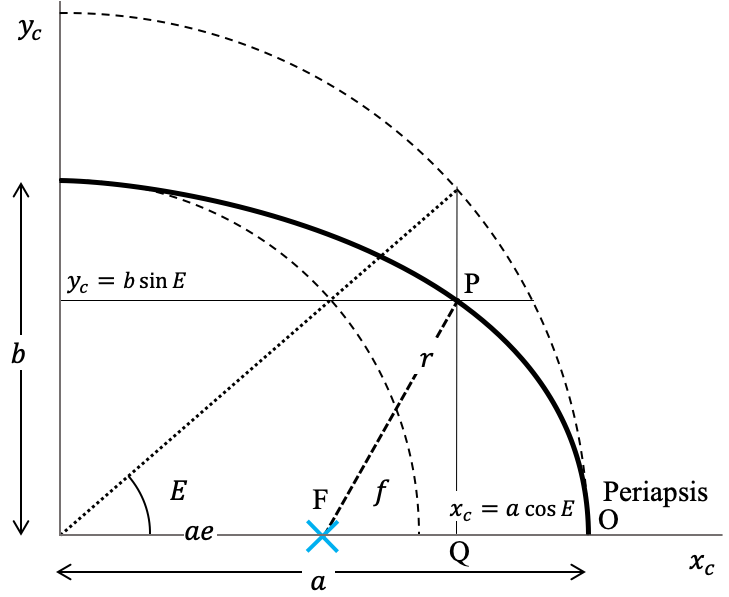
\includegraphics[width=0.5\textwidth]{./figures/square_anomalia_excentrica.png}
\caption{Definición de la anomalía excéntrica \(E\) y el método asociada
a ella para determinar la posición de los puntos sobre una
elipse.\label{fig:anomalia_excentrica}}
\end{figure}

¿Podemos escribir una ecuación para \(r\) en términos del parámetro
\(E\) análoga a la Ec. (\ref{eq:conica_ecuacion_cilindricas}) que nos da
\(r\) en función de \(f\)? ¡Sin duda alguna!

Considere el tríangulo entre los puntos FPQ en la
\autoref{fig:anomalia_excentrica}. El teorema de pitágoras en ese
triángulo se escribe:

\[
r^2=(a\cos E-ae)^2 + b^2\sin^2 E
\]

Teniendo en cuenta que \(b^2=a^2(1-e^2)\) y después de un poco de ágebra
obtenemos:

\begin{equation}
\label{eq:conica_anomalia_excentrica}
r=a(1-e\cos E)
\end{equation} que será una forma para representar la cónica alternativa
a la Ec. (\ref{eq:conica_anomalia_excentrica}) y que usaremos con
frecuencia en el libro.

Finalmente, la manipulación adecuada de las ecuaciones anteriores
permite escribir una relación explícita entre las anomalías verdadera
\(f\) y excéntrica \(E\) que será muy utilizada a lo largo de este libro
(ver problemas al final del capítulo):

\begin{equation}
\label{eq:fE}
\tan \frac{f}{2} = \sqrt{\frac{1+e}{1-e}} \tan \frac{E}{2}
\end{equation}
\vspace{-1em}

%%figcaption::hide::Anomalía verdadera $f$ como función de la anomalía excéntrica $E$ para una elipse.  La línea rayada corresponde a la aproximación $f\approx\sqrt{(1+e)/(1-e)}E$ que es valida en el caso $f\ll 1$.

%%hidecode


    \begin{center}

\begin{figure}[ht!]
\centering
    \adjustimage{max size={0.8\linewidth}{0.8\paperheight}}{combined_files/combined_400_0.png}
\caption{Anomalía verdadera $f$ como función de la anomalía excéntrica $E$ para una elipse.  La línea rayada corresponde a la aproximación $f\approx\sqrt{(1+e)/(1-e)}E$ que es valida en el caso $f\ll 1$.\label{fig:hide}}
\end{figure}

    \end{center}
%{ \hspace*{\fill} \\}
    
Un procedimiento similar al anterior, pero en el caso de la hipérbola,
permite escribir las coordenadas de los puntos de la curva en términos
de un nuevo parámetro \(F\):

\begin{equation}
\label{eq:hiperbola_parametrica_F}
\begin{array}{rcl}
x_c & = & a \cosh F\\
y_c & = & a \sinh F\\
\end{array}
\end{equation}

Por analogía con la elipse, \(F\) también es llamada la anomalía
excéntrica (aunque en este caso la interpretación geométrica de \(F\) no
es tan directa como en el caso de \(E\).)

La distancia al foco se puede escribir en términos de \(F\) como:

\begin{equation}
r = a(e\cosh F - 1)
\end{equation} y la relación entre la anomalía verdadera \(f\) y la
anomalía excéntrica \(F\) resulta ser:

\begin{equation}
\tanh \frac{f}{2} = \sqrt{\frac{e+1}{e-1}} \tanh \frac{F}{2}
\end{equation}
\vspace{-1em}

%%figcaption::hide::Anomalía excéntrica $F$ como función de la anomalía verdadera $f$ para una hipérbola. La línea punteada corresponde a la aproximación $F\approx\sqrt{(e-1)/(e+1)}f$.

%%hidecode


    \begin{center}

\begin{figure}[ht!]
\centering
    \adjustimage{max size={0.8\linewidth}{0.8\paperheight}}{combined_files/combined_402_0.png}
\caption{Anomalía excéntrica $F$ como función de la anomalía verdadera $f$ para una hipérbola. La línea punteada corresponde a la aproximación $F\approx\sqrt{(e-1)/(e+1)}f$.\label{fig:hide}}
\end{figure}

    \end{center}
%{ \hspace*{\fill} \\}
    


\hypertarget{area_conicas}{%
\subsection{Área de las cónicas}\label{area_conicas}}

Existe un último resultado de la geometría analítica de las cónicas que
es de interés para la mecánica celeste: el área encerrada por estas
curvas. Como veremos en el \autoref{problema_doscuerpos}, el área es
la única cantidad geométrica cuyo valor puede predicerse de forma exacta
como función del tiempo cuando describimos el movimiento de un cuerpo
respecto a un centro de atracción.
\begin{box_history}{Un poco de historia}{}{nofloat}
\small

\textbf{Newton, el área debajo de la hipérbola y la invención del
cálculo.} El cálculo del área encerrada por curvas arbitrarias
(cuadratura) es uno de los problemas clásicos de la geometría y en los
1600 uno de los que motivo la invención del cálculo infinitesimal (ver
\autoref{integrales}.)

\end{box_history}
En la \autoref{fig:conicas_area} se muestran las construcciones
geométricas que usaremos en las próximas sesiones para calcular el área
encerrada por elipses, hipérbolas y parábolas en función de las
anomalías definidas en las secciones anterioes y otros parámetros
geométricos de esas mismas cónicas.

\begin{figure}[t!]
\centering
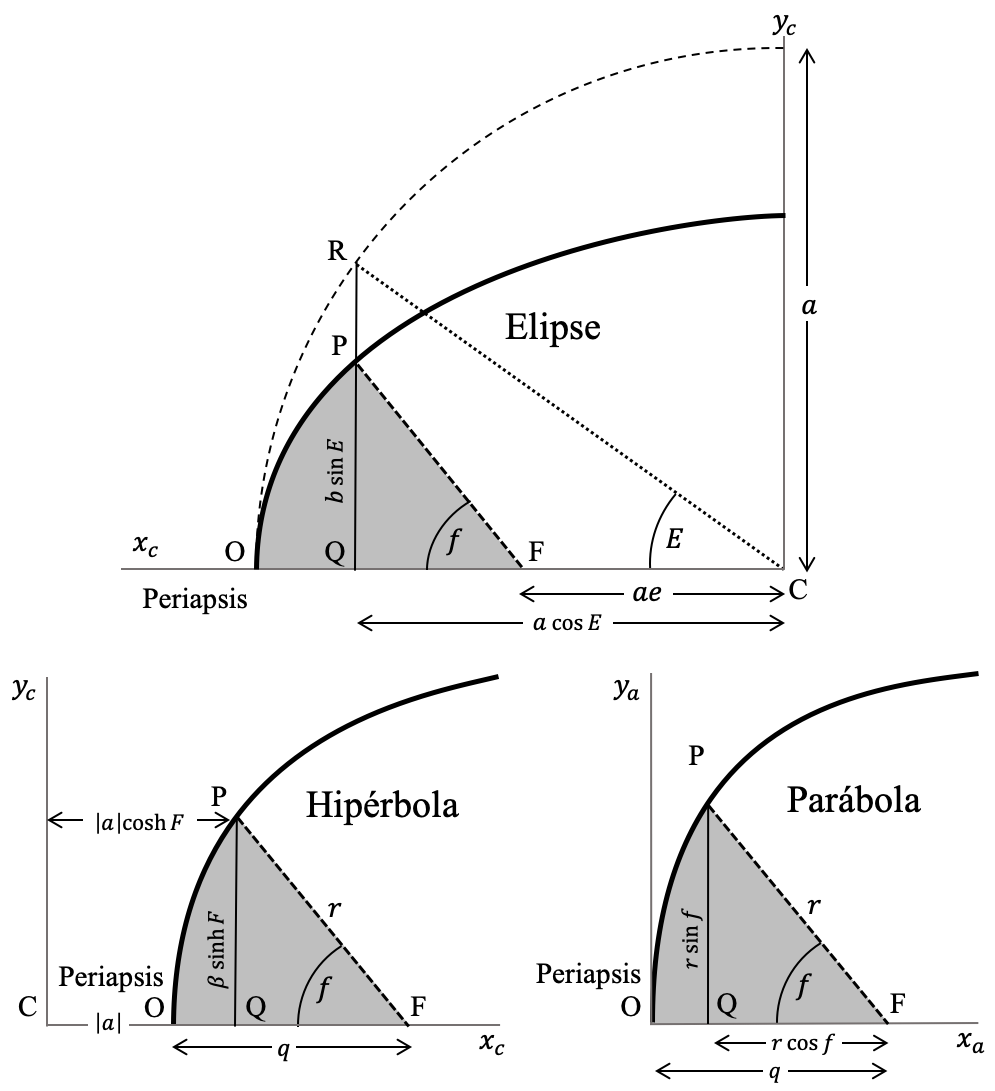
\includegraphics[width=1.0\textwidth]{./figures/square_area_conicas.png}
\caption{Construcción geométrica usada aquí para deducir la relación
entre las anomalías \(f\), \(E\) y \(F\) y el área del sector de cónica
(región sombreada).\label{fig:conicas_area}}
\end{figure}

En los tres casos el área del \emph{sector de cónica} PQF, que es el
área de interés para nosotros en la mecánica celeste, se puede siempre
escribir como la suma del segmento PQO y del triángulo PFQ:

\begin{equation}
\label{eq:area_sector}
\Delta A\equiv A_\mathrm{PQF}=A_\mathrm{PFQ}+A_\mathrm{PQO}
\end{equation}

El problema, en las tres cónicas consiste en calcular estas dos áreas
como función de las anomalías excéntricas (en el caso de la elipse y la
hipérbola y de la anomalía verdadera en el caso de la parábola.

\hypertarget{area_elipse}{%
\subsubsection{Área de un sector de elipse}\label{area_elipse}}

El área del triángulo en PFQ en la elipse (ver panel superior en
\autoref{fig:conicas_area}) se puede escribir en términos de la anomalía
excéntrica \(E\) como:

\begin{eqnarray}
\nonumber
A_\mathrm{PFQ} & = & \frac{1}{2} b\sin E (a\cos E-ae)\\
\label{eq:A_PFQ}
               & = & \frac{1}{2} ab\sin E\cos E - abe\sin E
\end{eqnarray}

Por otro lado, el área del segmento de elipse PQO se puede expresar como
la integral definida:

\[
A_\mathrm{PQO}=\int_{-a}^{x_c} y_c(x) \mathrm{d}x
\]

Por las propiedades geométricas de la elipse (ver
\autoref{conicas_anomalias}) la ordenada del punto P es
\(y_c(x)=(b/a)Y(x)\), donde \(Y\) es la correspondiente ordenada del
punto R sobre la circunferencia circunscrita en la elipse de radio \(a\)
. De esta manera el área del segmento de elipse se puede expresar en
términos del área de segmento de circulo RQO como:

\begin{equation}
\label{eq:A_PQO}
A_\mathrm{PQO}=\frac{1}{2}A_\mathrm{RQO}
\end{equation}

Por su parte:

\[
A_\mathrm{RQO}=A_\mathrm{RCO}-A_\mathrm{RCQ}
\] que a su vez se escriben en términos de \(E\) como:

\begin{equation}
\label{eq:A_RQO}
A_\mathrm{RQO}=\frac{1}{2}a^2 E-\frac{1}{2}a^2\sin E\cos E
\end{equation}

Reemplazando la Ec. (\ref{eq:A_RQO}) en la (\ref{eq:A_PQO}) y esta
última junto con la Ec. (\ref{eq:A_PFQ}) en la fórmula original (Ec.
\ref{eq:area_sector}) obetenmos finalmente:

\begin{equation}
\label{eq:area_sector_elipse}
\Delta A_\mathrm{elipse}=\frac{1}{2}ab(E-\sin E)
\end{equation}

Siendo la elipse la única figura cerrada entre las cónicas, es posible
calcular el área total encerrada por ella haciendo en la última ecuación
\(E=2\pi\):

\begin{equation}
\label{eq:area_elipse}
A_\mathrm{elipse}=\pi ab E
\end{equation}

\hypertarget{area_hiperbola}{%
\subsubsection{Área de un sector de hipérbola}\label{area_hiperbola}}

La construcción en la \autoref{fig:conicas_areas} permite, en el caso de
la hipérbola (ver panel inferior izquierdo) escribir las áreas de
interés en la Ec. (\ref{eq:area_sector}) como:

\begin{eqnarray}
\nonumber
A_\mathrm{PFQ} & = & \frac{1}{2}\beta\sinh F(|a|+q-|a|\cosh F)\\
\nonumber
A_\mathrm{PQO} & = & \int_{|a|}^{|a|\cosh F} \beta\sqrt{\frac{x^2}{a^2}-1}\;\mathrm{d}x
\end{eqnarray}

Para la última expresión usamos la ecuación de la hipérbola referida al
centro (ver Ec. \ref{eq:ecuacion_centro_hiperbola}).

Resolviendo la integral (ver problemas al final del capítulo), sumando
las dos áreas y teniendo en cuenta que \(q=|a|(e-1)\) obtenemos
finalmente el área del sector de hipérbola:

\begin{equation}
\label{eq:area_sector_hiperbola}
\Delta A_\mathrm{hiperbola}=\frac{1}{2}|a|\beta(e\sinh F-F)
\end{equation}

\hypertarget{area_paruxe1bola}{%
\subsubsection{Área de un sector de parábola}\label{area_paruxe1bola}}

De forma análoga a como lo hicimos con la hipérbola, podemos escribir
lás áreas que componen el sector de parábola en términos de la anomalía
verdadera \(f\) (ver panel inferior derecho en la
\autoref{fig:conicas_areas}):

\begin{eqnarray}
\nonumber
A_\mathrm{PFQ} & = & \frac{1}{2}r^2 \sin f\cos f\\
\nonumber
A_\mathrm{PQO} & = & \int_{0}^{q-r\cos f} \sqrt{2 p x}\;\mathrm{d}x
\end{eqnarray} donde en la integral hemos usado la ecuación de la
parábola con origen en el ápside \(y_a(x_a)^2=2px_a\) (ver Ec.
\ref{eq:ecuacion_apside_pe}).

A pesar de que estas expresiones parecen más fáciles de desarrollar
matemáticamente, en realidad encontrar una versión simplificada del área
del sector de parábola es más complicado de lo que es para el caso del
sector de elipse y el de hipérbola.

En términos llanos (sin simplificaciones trigonométricas), el área del
sector, que es la suma de las ecuaciones anteriores resulta ser:

\[
\Delta A_\mathrm{parabola}=\frac{1}{2}\frac{p^2\sin f\cos f}{(1+\cos f)^2}+\frac{p^2}{3}\left(\frac{1-\cos f}{1+\cos f}\right)^{3/2}
\] donde hemos usado la ecuación de la parábola en coordenadas
cilíndricas, \(r=p/(1+\cos f)\) y el hecho que \(q=p/2\).

La fracción en el segundo término del lado derecho se puede escribir
como:

\[
\frac{1-\cos f}{1+\cos f}=\tan\frac{f}{2}
\] y esto nos ofrece una clave de cómo simplificar el primer término:
escribiéndo \(\sin f\) y \(\cos f\) en términos de \(\tan(f/2)\):

\begin{eqnarray}
\sin f & = & \frac{2\tan\frac{f}{2}}{1+\tan^2\frac{f}{2}}\\
\cos f & = & \frac{1-\tan^2\frac{f}{2}}{1+\tan^2\frac{f}{2}}\\
\end{eqnarray}

Reemplazando, el área del sector de parábola queda:

\[
\Delta A_\mathrm{parabola}=\frac{1}{4} p^2\tan\frac{f}{2}\left(1-\tan^2\frac{f}{2}\right)+\frac{p^2}{6}\tan^3\frac{f}{2}
\] y simplifando obtenemos finalmente:

\begin{equation}
\label{eq:area_sector_parabola}
\Delta A_\mathrm{parabola}=\frac{1}{4}p^2\left(\tan\frac{f}{2}+\frac{1}{3}\tan^3\frac{f}{2}\right)
\end{equation}



\hypertarget{conicas_espacio}{%
\subsection{Cónicas en el espacio}\label{conicas_espacio}}

En las secciones anteriores desarrollamos todas las posibles
representaciones algebraicas de las curvas cónicas sobre el plano en el
que están definidas. En esta sesión daremos el salto a tres dimensiones
y resolveremos la pregunta de ¿cuál es la representación algebraica o
geométrica más general de las cónicas en el espacio?

En la \autoref{conicas_rotacion_plano} habíamos visto que es
posible, partiendo de la descripción algebraica de la cónica en un
sistema de coordenadas referido a su eje de simetría y que llamaremos en
lo sucesivo el \emph{sistema de referencia natural de la cónica},
aplicar una rotación sobre el plano para obtener la ecuación más general
de la cónica sobre ese mismo plano. El salto al espacio de tres
dimensiones es simplemente una generalización de este procedimiento.

\hypertarget{angulos_euler}{%
\subsection{Ángulos de Euler}\label{angulos_euler}}

Partiendo del sistema de referencia natural de la cónica, es posible
orientar de forma arbitraria la curva en el espacio realizando en total
tres rotaciones \emph{independientes} (ver \autoref{fig:angulos_euler}.)
Los ángulos en los que se realizan esas rotaciones, y que llamaremos en
este texto \((\Omega,i,\omega)\), se conocen universalmente como los
\textbf{ángulos de Euler}.

\begin{figure}[t!]
\centering
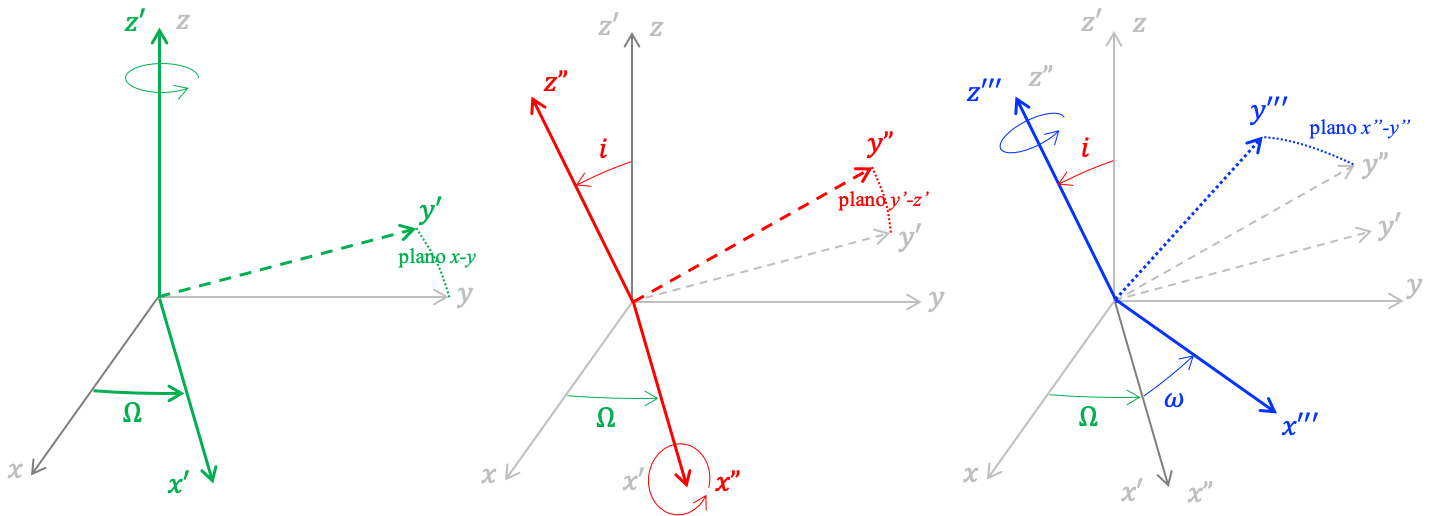
\includegraphics[width=1\textwidth]{./figures/horizontal_angulos_euler.png}
\caption{Secuencia de rotaciones que permiten pasar del sistema natural
de ejes de la cónica \(x-y-z\) a un sistema con una orientación
arbitraria \(x'''-y'''-z'''\)\label{fig:angulos_euler}}
\end{figure}

La secuencia de rotaciones mostradas en la \autoref{fig:aungulos_euler}
se puede describir cualitativamente como:

\begin{enumerate}
\def\labelenumi{\arabic{enumi}.}
\item
  Rotación del sistema original \(x-y-z\) (sistema natural) en un ángulo
  \(\Omega\) alrededor del eje z, para obtener un nuevo sistema de ejes
  \(x'-y'-z'\)
\item
  Rotación del sistema \(x'-y'-z'\) en un ángulo \(i\) alrededor del eje
  \(z'\), para obtener un nuevo sistema de ejes \(x''-y''-z''\)
\item
  Rotación del sistema \(x''-y''-z''\) en un ángulo \(\omega\) alrededor
  del eje \(z''\), para obtener un nuevo sistema de ejes
  \(x'''-y'''-z'''\).
\end{enumerate}

Al sistema de ejes final lo llamamos el \emph{sistema de coordenadas del
observador}.

Usando la representación matricial de las rotaciones en el plano de la
Ec. (\ref{eq:rotacion2d_matricial}), la relación entre las coordenadas
del observador y las coordenadas naturales de las cónicas será:

\begin{equation}
\label{eq:rotacion3d_observador_R}
\left(
\begin{array}{c}
x''' \\
y''' \\
z'''
\end{array}
\right)
= R_z(\omega) R_x(i) R_z(\Omega)
\left(
\begin{array}{c}
x \\
y \\
z
\end{array}
\right)
\end{equation}

Si usamos la definición de las matrices de rotación de la Ec.
(\ref{eq:matriz_rotacion2d}):

\[
\label{matrix-inverted} \left( \begin{array}{c}
   x''' \\
   y''' \\
   z'''
   \end{array}  \right)= \left( \begin{array}{ccc}
   \mathrm{c} \omega & \mathrm{s} \omega & 0\\
   -\mathrm{s} \omega & \mathrm{c} \omega & 0\\  
   0 & 0 & 1
   \end{array} \right) \left( \begin{array}{ccc}
   1 & 0 & 0\\
   0 & \mathrm{c} i & \mathrm{s} i\\  
   0 & -\mathrm{s} i & \mathrm{c} i
   \end{array} \right) \left( \begin{array}{ccc}
   \mathrm{c} \Omega & \mathrm{s} \Omega & 0\\
   -\mathrm{s} \Omega & \mathrm{c} \Omega & 0\\  
   0 & 0 & 1
   \end{array} \right)
   \left( \begin{array}{c}
   x \\
   y \\
   z
   \end{array}  \right)
\] donde se ha abreviado \(\mathrm{c}\theta\equiv\cos\theta\) y
\(\mathrm{s}\theta\equiv\sin\theta\).

Al realizar las multiplicaciones matriciales explícitas queda:

\begin{equation}
\label{eq:rotacion3d_observador_M}
\left( \begin{array}{c}
   x''' \\
   y''' \\
   z'''
   \end{array}  \right)= 
   {\cal M}(\Omega,i,\omega)
   \left( \begin{array}{c}
   x \\
   y \\
   z
   \end{array}  \right)
\end{equation} donde la matriz de rotación en tres dimensiones,

\begin{equation}
\label{eq:matrizM_definicion}
{\cal M}(\omega,i,\Omega)\equiv R_z(\omega) R_x(i) R_z(\Omega)
\end{equation} se escribe explícitamente como:

\begin{equation}
\label{eq:matrizM_explicita}
{\cal M}(\omega,i,\Omega)=
   \left( \begin{array}{ccc}
   \mathrm{c} \omega\;\mathrm{c} \Omega - \mathrm{c} i\;\mathrm{s} \omega\; \mathrm{s} \Omega  & \mathrm{c} \omega\; \mathrm{s} \Omega + \mathrm{c} \Omega\; \mathrm{c} i\; \mathrm{s} \omega & \mathrm{s} i\; \mathrm{s} \omega \\
   -\mathrm{c} \Omega\; \mathrm{s} \omega - \mathrm{s} \Omega\; \mathrm{c} i\; \mathrm{c} \omega & -\mathrm{s} \Omega\; \mathrm{s} \omega + \mathrm{c} \Omega\; \mathrm{c} i\; \mathrm{c} \omega & \mathrm{s} i\; \mathrm{c} \Omega \\
   \mathrm{s} \Omega\; \mathrm{s} i & -\mathrm{c} \Omega\; \mathrm{s} i & \mathrm{c} i \\ 
   \end{array} \right)
\end{equation}

Por ser \({\cal M}\) el producto de matrices de unitarias (Ec.
\ref{eq:matrizM_definicion}), ella es en sí misma una matriz unitaria,
es decir \(\mathrm det{\cal M}=1\), pero más importante:

\[
{\cal M}^{-1}={\cal M}^\mathrm{T}
\] explícitamente,

\begin{equation}
\label{eq:matrizM_explicita_transpuesta}
{\cal M}(\omega,i,\Omega)^\mathrm{T}=
   \left( \begin{array}{ccc}
   \mathrm{c} \omega \;\mathrm{c} \Omega - \mathrm{c} i \;\mathrm{s} \Omega \;\mathrm{s} \omega  & -\mathrm{c} \Omega \;\mathrm{s} \omega - \;\mathrm{c} \omega \;\mathrm{c} i \;\mathrm{s} \Omega & \mathrm{s} i \;\mathrm{s} \Omega \\
   \mathrm{c} \omega \;\mathrm{s} \Omega + \mathrm{s} \omega \;\mathrm{c} i \;\mathrm{c} \Omega & -\mathrm{s} \Omega \;\mathrm{s} \omega + \mathrm{c} \omega \;\mathrm{c} i \;\mathrm{c} \Omega & \mathrm{s} i \;\mathrm{c} \omega \\
   \mathrm{s} \omega \;\mathrm{s} i & \mathrm{c} \omega \;\mathrm{s} i & \mathrm{c} i \\ 
   \end{array} \right)
\end{equation}

A la inversa, las coordenadas naturales de la cónica \((x,y,z)\) se
pueden obtener de las coordenadas del observador, invirtiendo la Ec.
(\ref{eq:rotacion3d_observador}):

\begin{equation}
\label{eq:rotacion3d_natural_R}
\left(
\begin{array}{c}
x \\
y \\
z
\end{array}
\right)
= R_z(-\Omega) R_x(-i) R_y(-\omega) 
\left(
\begin{array}{c}
x''' \\
y''' \\
z'''
\end{array}
\right)
\end{equation} o equivalentemente, usando la forma explícita en la Ec.
(\ref{eq:rotacion3d_observador_M}) y aprovechando las propiedades de la
matriz de rotación en tres dimensiones \(\cal M\):

\begin{equation}
\label{eq:rotacion3d_natural_M}
\left( \begin{array}{c}
   x \\
   y \\
   z
   \end{array}  \right)= 
   {\cal M}^\mathrm{T}
   \left( \begin{array}{c}
   x''' \\
   y''' \\
   z'''
   \end{array}  \right)
\end{equation}

\hypertarget{matrices_rotacion_generales}{%
\subsection{Matrices de rotación
generales}\label{matrices_rotacion_generales}}

Usando \texttt{SPICE} podemos construir la matriz de rotación en tres
dimensiones \({\cal M}\) por dos medios distintos. El primero es usar la
rutina \texttt{rotate} que habíamos introducido en el Alg.
(\ref{code:spice_rotate}):

    \begin{code}{}{}\begin{Verbatim}[fontsize=\small,commandchars=\\\{\}]
\PY{c+c1}{\PYZsh{}Angulos}
\PY{k+kn}{from} \PY{n+nn}{numpy} \PY{k}{import} \PY{n}{pi}
\PY{n}{Omega}\PY{o}{=}\PY{n}{pi}\PY{o}{/}\PY{l+m+mi}{6}
\PY{n}{omega}\PY{o}{=}\PY{n}{pi}\PY{o}{/}\PY{l+m+mi}{3}
\PY{n}{i}\PY{o}{=}\PY{n}{pi}\PY{o}{/}\PY{l+m+mi}{4}

\PY{c+c1}{\PYZsh{}Matrices indiduales}
\PY{k+kn}{from} \PY{n+nn}{spiceypy} \PY{k}{import} \PY{n}{rotate}
\PY{n}{RzOmega}\PY{o}{=}\PY{n}{rotate}\PY{p}{(}\PY{n}{Omega}\PY{p}{,}\PY{l+m+mi}{3}\PY{p}{)}
\PY{n}{Rxi}\PY{o}{=}\PY{n}{rotate}\PY{p}{(}\PY{n}{i}\PY{p}{,}\PY{l+m+mi}{1}\PY{p}{)}
\PY{n}{Rzomega}\PY{o}{=}\PY{n}{rotate}\PY{p}{(}\PY{n}{omega}\PY{p}{,}\PY{l+m+mi}{3}\PY{p}{)}
\end{Verbatim}

%%

\end{code}

La matriz de rotación en tres dimensiones \({\cal M}\), de acuerdo con
su definición en la Ec. (\ref{eq:matrizM_definicion}), puede obtenerse
aplicando sucesivamente la rutina de multiplicación de matrices
\texttt{mxm}:

    \begin{code}{Algoritmo}{code:calculo_M_explicito}\begin{Verbatim}[fontsize=\small,commandchars=\\\{\}]
\PY{k+kn}{from} \PY{n+nn}{spiceypy} \PY{k}{import} \PY{n}{mxm}
\PY{n}{M}\PY{o}{=}\PY{n}{mxm}\PY{p}{(}\PY{n}{Rzomega}\PY{p}{,}\PY{n}{mxm}\PY{p}{(}\PY{n}{Rxi}\PY{p}{,}\PY{n}{RzOmega}\PY{p}{)}\PY{p}{)}
\end{Verbatim}

%%

\end{code}
\vspace{-1em}

%%hidecode


    \begin{Verbatim}[fontsize=\small,commandchars=\\\{\}]
M = 
[[ 0.12682648  0.78033009  0.61237244]
 [-0.9267767  -0.12682648  0.35355339]
 [ 0.35355339 -0.61237244  0.70710678]]
\end{Verbatim}

Existe sin embargo una rutina compacta y mucho más general en
\texttt{SPICE} que permite calcular la matriz rotación de cualquier
sucesión de rotaciones en el espacio, no solamente la que usamos aquí.

Para ello podemos definir una matriz de rotación general \({\cal R}\)
resultante de aplicar rotaciones sucesivas \(\theta_i\) alrededor del
eje \(\hat{e}_k\), \(\theta_j\) alrededor del eje \(\hat{e}_j\) y
\(\theta_i\) alrededor del eje \(\hat{e}_i\) como:

\[
{\cal R}(\theta_i,\theta_j,\theta_k,i,j,k)\equiv R_{i}(\theta_i)R_{j}(\theta_j)R_{k}(\theta_k)
\]

En términos de esta matriz general, la matriz de rotación
\emph{canónica} \({\cal M}\) presentada en la
\autoref{angulos_euler} se escribe:

\[
{\cal M}={\cal R}(\omega,i,\Omega,3,1,3)
\]

En el paquete \texttt{SPICE} la rotación general \({\cal R}\) se
implementa con la rutina \texttt{eul2m} que podemos usar para obtener
\(\cal M\) como:

    \begin{code}{Algoritmo}{code:calculo_M_general}\begin{Verbatim}[fontsize=\small,commandchars=\\\{\}]
\PY{k+kn}{from} \PY{n+nn}{spiceypy} \PY{k}{import} \PY{n}{eul2m}
\PY{n}{M}\PY{o}{=}\PY{n}{eul2m}\PY{p}{(}\PY{n}{omega}\PY{p}{,}\PY{n}{i}\PY{p}{,}\PY{n}{Omega}\PY{p}{,}\PY{l+m+mi}{3}\PY{p}{,}\PY{l+m+mi}{1}\PY{p}{,}\PY{l+m+mi}{3}\PY{p}{)}
\end{Verbatim}

%%

\end{code}
\vspace{-1em}

%%hidecode


    \begin{Verbatim}[fontsize=\small,commandchars=\\\{\}]
M = 
[[ 0.12682648  0.78033009  0.61237244]
 [-0.9267767  -0.12682648  0.35355339]
 [ 0.35355339 -0.61237244  0.70710678]]
\end{Verbatim}

Naturalmente el resultado coincide con el obtenido en el Alg.
(\ref{code:calculo_M_explicito}). Podemos ahora verificar la unitariedad
de \(\cal M\) calculando su determinante, su inversa (calculada numérica
y usando la propiedad en la Ec. \ref{eq:rotacion3d_natural_R}) y su
transpuesta:

    \begin{code}{}{}\begin{Verbatim}[fontsize=\small,commandchars=\\\{\}]
\PY{c+c1}{\PYZsh{}Determinante}
\PY{k+kn}{from} \PY{n+nn}{numpy}\PY{n+nn}{.}\PY{n+nn}{linalg} \PY{k}{import} \PY{n}{det}
\PY{n}{detM}\PY{o}{=}\PY{n}{det}\PY{p}{(}\PY{n}{M}\PY{p}{)}

\PY{c+c1}{\PYZsh{}Inversa}
\PY{k+kn}{from} \PY{n+nn}{numpy}\PY{n+nn}{.}\PY{n+nn}{linalg} \PY{k}{import} \PY{n}{inv}
\PY{n}{Minv}\PY{o}{=}\PY{n}{inv}\PY{p}{(}\PY{n}{M}\PY{p}{)}

\PY{c+c1}{\PYZsh{}Inversa por definicion}
\PY{n}{Minv\PYZus{}def}\PY{o}{=}\PY{n}{eul2m}\PY{p}{(}\PY{o}{\PYZhy{}}\PY{n}{Omega}\PY{p}{,}\PY{o}{\PYZhy{}}\PY{n}{i}\PY{p}{,}\PY{o}{\PYZhy{}}\PY{n}{omega}\PY{p}{,}\PY{l+m+mi}{3}\PY{p}{,}\PY{l+m+mi}{1}\PY{p}{,}\PY{l+m+mi}{3}\PY{p}{)}

\PY{c+c1}{\PYZsh{}Transpuesta}
\PY{n}{MT}\PY{o}{=}\PY{n}{M}\PY{o}{.}\PY{n}{transpose}\PY{p}{(}\PY{p}{)}
\end{Verbatim}

%%

\end{code}

    \begin{code}{}{}\begin{Verbatim}[fontsize=\small,commandchars=\\\{\}]
\PY{n+nb}{print}\PY{p}{(}\PY{n}{f}\PY{l+s+s2}{\PYZdq{}}\PY{l+s+s2}{det(M) = }\PY{l+s+si}{\PYZob{}detM:g\PYZcb{}}\PY{l+s+s2}{\PYZdq{}}\PY{p}{)}
\PY{n+nb}{print}\PY{p}{(}\PY{n}{f}\PY{l+s+s2}{\PYZdq{}}\PY{l+s+s2}{inversa M (numérica) = }\PY{l+s+se}{\PYZbs{}n}\PY{l+s+si}{\PYZob{}Minv\PYZcb{}}\PY{l+s+s2}{\PYZdq{}}\PY{p}{)}
\PY{n+nb}{print}\PY{p}{(}\PY{n}{f}\PY{l+s+s2}{\PYZdq{}}\PY{l+s+s2}{inversa M (definición) = }\PY{l+s+se}{\PYZbs{}n}\PY{l+s+si}{\PYZob{}Minv\PYZus{}def\PYZcb{}}\PY{l+s+s2}{\PYZdq{}}\PY{p}{)}
\PY{n+nb}{print}\PY{p}{(}\PY{n}{f}\PY{l+s+s2}{\PYZdq{}}\PY{l+s+s2}{transpuesta M = }\PY{l+s+se}{\PYZbs{}n}\PY{l+s+si}{\PYZob{}MT\PYZcb{}}\PY{l+s+s2}{\PYZdq{}}\PY{p}{)}
\end{Verbatim}

%%

\end{code}

    \begin{Verbatim}[fontsize=\small,commandchars=\\\{\}]
det(M) = 1
inversa M (numérica) = 
[[ 0.12682648 -0.9267767   0.35355339]
 [ 0.78033009 -0.12682648 -0.61237244]
 [ 0.61237244  0.35355339  0.70710678]]
inversa M (definición) = 
[[ 0.12682648 -0.9267767   0.35355339]
 [ 0.78033009 -0.12682648 -0.61237244]
 [ 0.61237244  0.35355339  0.70710678]]
transpuesta M = 
[[ 0.12682648 -0.9267767   0.35355339]
 [ 0.78033009 -0.12682648 -0.61237244]
 [ 0.61237244  0.35355339  0.70710678]]
\end{Verbatim}

\hypertarget{grafico_conica_rotada_espacio}{%
\subsection{Gráfico de una cónica rotada en el
espacio}\label{grafico_conica_rotada_espacio}}

Con estos elementos a la mano podemos escribir algoritmos para, usando
las ecuaciones encontradas en la
\autoref{grafico_conica_rotada_plano} y los algoritmos de la
\autoref{grafico_conica_rotada_plano}, representar gráficamente una
cónica en el espacio.

Comenzamos por obtener los puntos de la cónica en su sistema natural de
coordenadas (plano de la cónica, origen en el foco, semieje \(x+\)
apuntando hacia el periapsis) usando para ello la rutina
\texttt{puntos\_conica} que habíamos introducido en el Alg.
(\ref{code:puntos_conica}):

    \begin{code}{}{}\begin{Verbatim}[fontsize=\small,commandchars=\\\{\}]
\PY{k+kn}{from} \PY{n+nn}{pymcel}\PY{n+nn}{.}\PY{n+nn}{export} \PY{k}{import} \PY{n}{puntos\PYZus{}conica}
\PY{n}{p}\PY{o}{=}\PY{l+m+mf}{10.0}
\PY{n}{e}\PY{o}{=}\PY{l+m+mf}{0.8}
\PY{n}{xs}\PY{p}{,}\PY{n}{ys}\PY{p}{,}\PY{n}{zs}\PY{o}{=}\PY{n}{puntos\PYZus{}conica}\PY{p}{(}\PY{n}{p}\PY{p}{,}\PY{n}{e}\PY{p}{)}
\end{Verbatim}

%%

\end{code}

Ahora podemos rotar los puntos de la cónica usando la matriz \texttt{M}
calculada en el Alg. (\ref{code:calculo_M_general}). Para hacerlo nos
apoyaremos nuevamente en la rutina general \texttt{rota\_puntos} que
habíamos introducido antes en el Alg. (\ref{cod:rota_puntos}):

    \begin{code}{}{}\begin{Verbatim}[fontsize=\small,commandchars=\\\{\}]
\PY{k+kn}{from} \PY{n+nn}{pymcel}\PY{n+nn}{.}\PY{n+nn}{export} \PY{k}{import} \PY{n}{rota\PYZus{}puntos}
\PY{n}{xppps}\PY{p}{,}\PY{n}{yppps}\PY{p}{,}\PY{n}{zppps}\PY{o}{=}\PY{n}{rota\PYZus{}puntos}\PY{p}{(}\PY{n}{M}\PY{p}{,}\PY{n}{xs}\PY{p}{,}\PY{n}{ys}\PY{p}{,}\PY{n}{zs}\PY{p}{)}
\end{Verbatim}

%%

\end{code}

Una gráfica en tres dimensiones de la cónica en su plano natural y en
los ejes rotados se puede realizar usando el siguiente código:
%%HIDE%%
    \begin{code}{Algoritmo}{code:4_Fundamentos_12}\begin{Verbatim}[fontsize=\small,commandchars=\\\{\}]
\PY{k+kn}{import} \PY{n+nn}{matplotlib}\PY{n+nn}{.}\PY{n+nn}{pyplot} \PY{k}{as} \PY{n+nn}{plt}
\PY{k+kn}{from} \PY{n+nn}{mpl\PYZus{}toolkits}\PY{n+nn}{.}\PY{n+nn}{mplot3d} \PY{k}{import} \PY{n}{Axes3D}
\PY{n}{fig}\PY{o}{=}\PY{n}{plt}\PY{o}{.}\PY{n}{figure}\PY{p}{(}\PY{p}{)}
\PY{n}{ax}\PY{o}{=}\PY{n}{fig}\PY{o}{.}\PY{n}{gca}\PY{p}{(}\PY{n}{projection}\PY{o}{=}\PY{l+s+s1}{\PYZsq{}}\PY{l+s+s1}{3d}\PY{l+s+s1}{\PYZsq{}}\PY{p}{)}

\PY{c+c1}{\PYZsh{}Gráfica de los puntos originales}
\PY{n}{ax}\PY{o}{.}\PY{n}{plot}\PY{p}{(}\PY{n}{xs}\PY{p}{,}\PY{n}{ys}\PY{p}{,}\PY{n}{zs}\PY{p}{,}\PY{l+s+s1}{\PYZsq{}}\PY{l+s+s1}{k\PYZhy{}\PYZhy{}}\PY{l+s+s1}{\PYZsq{}}\PY{p}{)}

\PY{c+c1}{\PYZsh{}Gráfica de la cónica rotada}
\PY{n}{ax}\PY{o}{.}\PY{n}{plot}\PY{p}{(}\PY{n}{xppps}\PY{p}{,}\PY{n}{yppps}\PY{p}{,}\PY{n}{zppps}\PY{p}{,}\PY{l+s+s1}{\PYZsq{}}\PY{l+s+s1}{b\PYZhy{}}\PY{l+s+s1}{\PYZsq{}}\PY{p}{)}

\PY{c+c1}{\PYZsh{}Decoración}
\PY{n}{ax}\PY{o}{.}\PY{n}{set\PYZus{}xlabel}\PY{p}{(}\PY{l+s+s2}{\PYZdq{}}\PY{l+s+s2}{\PYZdl{}x\PYZdl{}}\PY{l+s+s2}{\PYZdq{}}\PY{p}{)}
\PY{n}{ax}\PY{o}{.}\PY{n}{set\PYZus{}ylabel}\PY{p}{(}\PY{l+s+s2}{\PYZdq{}}\PY{l+s+s2}{\PYZdl{}y\PYZdl{}}\PY{l+s+s2}{\PYZdq{}}\PY{p}{)}
\PY{n}{ax}\PY{o}{.}\PY{n}{set\PYZus{}zlabel}\PY{p}{(}\PY{l+s+s2}{\PYZdq{}}\PY{l+s+s2}{\PYZdl{}z\PYZdl{}}\PY{l+s+s2}{\PYZdq{}}\PY{p}{)}

\PY{k+kn}{from} \PY{n+nn}{pymcel}\PY{n+nn}{.}\PY{n+nn}{plot} \PY{k}{import} \PY{n}{fija\PYZus{}ejes3d\PYZus{}proporcionales}
\PY{n}{fija\PYZus{}ejes3d\PYZus{}proporcionales}\PY{p}{(}\PY{n}{ax}\PY{p}{)}\PY{p}{;}
\PY{n}{fig}\PY{o}{.}\PY{n}{tight\PYZus{}layout}\PY{p}{(}\PY{p}{)}\PY{p}{;}
\end{Verbatim}

%%

\tcblower
\footnotesize
\em ver Figura \ref{fig:code:4_Fundamentos_12}
\end{code}

    \begin{center}

\begin{figure}[ht!]
\centering
    \adjustimage{max size={0.8\linewidth}{0.8\paperheight}}{combined_files/combined_460_0.png}
\caption{Figura correspondiente al código \ref{code:4_Fundamentos_12}.\label{fig:code:4_Fundamentos_12}}
\end{figure}

    \end{center}
%{ \hspace*{\fill} \\}
    
\hypertarget{elementos_orbitales}{%
\subsection{Elementos orbitales}\label{elementos_orbitales}}

Partiendo de las ecuaciones paramétricas de la cónica en su plano
natural (Ecs. \ref{eq:conica_parametricas_f} y
\ref{eq:conica_ecuacion_cilindricas}):

\begin{eqnarray}
\nonumber
x''' & = & \frac{p\cos f}{1+e\cos f}\\
\nonumber
y''' & = & \frac{p\sin f}{1+e\cos f}\\
\nonumber
z''' & = & 0
\end{eqnarray} y usando las expresiones explícitas para la rotación en
tres dimensiones dadas por las Ecs. (\ref{eq:rotacion3d_natural_M}) y
(\ref{eq:matrizM_explicita_transpuesta}), podemos escribir las
ecuaciones paramétricas generales de una cónica en el espacio:

\begin{equation}
\label{eq:elementos_estado_f}
\begin{array}{rcl}
x & = & r[\cos \Omega \cos(\omega+f) - \cos i \sin \Omega \sin(\omega+f)]\\
y & = & r[\sin \Omega \cos(\omega+f) + \cos i \cos \Omega \sin(\omega+f)]\\
z & = & r[\cos f\sin \omega \sin i + \sin f \cos \omega \sin i]\\ 
\end{array}
\end{equation} donde \(r=p/(1+e\cos f)\)

Vemos aquí entonces que para específicar la posición de cualquier punto
sobre una cónica, independiente de su orientación espacial, hace falta
indicar el valor de 6 parámetros: \(p\), \(e\), \(i\), \(\Omega\),
\(\omega\) y \(f\). A estas cantidades las llamamos en mecánica celeste
los \textbf{elementos orbitales clásicos} y volveremos sobre ellos en el
\autoref{problema_doscuerpos}.

En realidad, de los 6 elementos orbitales clásicos, 5 de ellos
\((p,e,i,\Omega,\omega)\) permiten especificar el tamaño, forma y
orientación de la cónica y son compartidos por todos los puntos que
definen la curva. El último elemento, \(f\) permite especificar la
posición de un punto específico.

Usando los elementos orbitales clásicos podemos dibujar una cónica en el
espacio usando un algoritmo más directo que el que usamos en la
\autoref{grafico_conica_rotada_espacio}. Para ello hemos diseñado la
rutina \texttt{conica\_de\_elementos}:

    \begin{code}{Algoritmo}{code:conica_de_elementos}\begin{Verbatim}[fontsize=\small,commandchars=\\\{\}]
\PY{k}{def} \PY{n+nf}{conica\PYZus{}de\PYZus{}elementos}\PY{p}{(}\PY{n}{p}\PY{o}{=}\PY{l+m+mf}{10.0}\PY{p}{,}\PY{n}{e}\PY{o}{=}\PY{l+m+mf}{0.8}\PY{p}{,}\PY{n}{i}\PY{o}{=}\PY{l+m+mf}{0.0}\PY{p}{,}\PY{n}{Omega}\PY{o}{=}\PY{l+m+mf}{0.0}\PY{p}{,}\PY{n}{omega}\PY{o}{=}\PY{l+m+mf}{0.0}\PY{p}{,}
                        \PY{n}{df}\PY{o}{=}\PY{l+m+mf}{0.1}\PY{p}{,}
                        \PY{n}{elev}\PY{o}{=}\PY{l+m+mi}{30}\PY{p}{,}\PY{n}{azim}\PY{o}{=}\PY{l+m+mi}{60}\PY{p}{,}
                        \PY{n}{figreturn}\PY{o}{=}\PY{k+kc}{False}\PY{p}{)}\PY{p}{:}

    \PY{c+c1}{\PYZsh{}Convierte elementos angulares en radianes}
    \PY{k+kn}{from} \PY{n+nn}{numpy} \PY{k}{import} \PY{n}{pi}
    \PY{n}{p}\PY{o}{=}\PY{n+nb}{float}\PY{p}{(}\PY{n}{p}\PY{p}{)}
    \PY{n}{e}\PY{o}{=}\PY{n+nb}{float}\PY{p}{(}\PY{n}{e}\PY{p}{)}
    \PY{n}{i}\PY{o}{=}\PY{n+nb}{float}\PY{p}{(}\PY{n}{i}\PY{p}{)}\PY{o}{*}\PY{n}{pi}\PY{o}{/}\PY{l+m+mi}{180}
    \PY{n}{Omega}\PY{o}{=}\PY{n+nb}{float}\PY{p}{(}\PY{n}{Omega}\PY{p}{)}\PY{o}{*}\PY{n}{pi}\PY{o}{/}\PY{l+m+mi}{180}
    \PY{n}{omega}\PY{o}{=}\PY{n+nb}{float}\PY{p}{(}\PY{n}{omega}\PY{p}{)}\PY{o}{*}\PY{n}{pi}\PY{o}{/}\PY{l+m+mi}{180}
    
    \PY{c+c1}{\PYZsh{}Compute fmin,fmax}
    \PY{k}{if} \PY{n}{e}\PY{o}{\PYZlt{}}\PY{l+m+mi}{1}\PY{p}{:}
        \PY{n}{fmin}\PY{o}{=}\PY{o}{\PYZhy{}}\PY{n}{pi}
        \PY{n}{fmax}\PY{o}{=}\PY{n}{pi}
    \PY{k}{elif} \PY{n}{e}\PY{o}{\PYZgt{}}\PY{l+m+mi}{1}\PY{p}{:}
        \PY{k+kn}{from} \PY{n+nn}{numpy} \PY{k}{import} \PY{n}{arccos}
        \PY{n}{psi}\PY{o}{=}\PY{n}{arccos}\PY{p}{(}\PY{l+m+mi}{1}\PY{o}{/}\PY{n}{e}\PY{p}{)}
        \PY{n}{fmin}\PY{o}{=}\PY{o}{\PYZhy{}}\PY{n}{pi}\PY{o}{+}\PY{n}{psi}\PY{o}{+}\PY{n}{df}
        \PY{n}{fmax}\PY{o}{=}\PY{n}{pi}\PY{o}{\PYZhy{}}\PY{n}{psi}\PY{o}{\PYZhy{}}\PY{n}{df}
    \PY{k}{else}\PY{p}{:}
        \PY{n}{fmin}\PY{o}{=}\PY{o}{\PYZhy{}}\PY{n}{pi}\PY{o}{+}\PY{n}{df}
        \PY{n}{fmax}\PY{o}{=}\PY{n}{pi}\PY{o}{\PYZhy{}}\PY{n}{df}
            
    \PY{c+c1}{\PYZsh{}Valores del ángulo}
    \PY{k+kn}{from} \PY{n+nn}{numpy} \PY{k}{import} \PY{n}{linspace}\PY{p}{,}\PY{n}{pi}
    \PY{n}{fs}\PY{o}{=}\PY{n}{linspace}\PY{p}{(}\PY{n}{fmin}\PY{p}{,}\PY{n}{fmax}\PY{p}{,}\PY{l+m+mi}{500}\PY{p}{)}

    \PY{c+c1}{\PYZsh{}Distancia al periapsis}
    \PY{n}{q}\PY{o}{=}\PY{n}{p}\PY{o}{/}\PY{p}{(}\PY{l+m+mi}{1}\PY{o}{+}\PY{n}{e}\PY{p}{)}

    \PY{c+c1}{\PYZsh{}Distancia al foco}
    \PY{k+kn}{from} \PY{n+nn}{numpy} \PY{k}{import} \PY{n}{sin}\PY{p}{,}\PY{n}{cos}
    \PY{n}{rs}\PY{o}{=}\PY{n}{p}\PY{o}{/}\PY{p}{(}\PY{l+m+mi}{1}\PY{o}{+}\PY{n}{e}\PY{o}{*}\PY{n}{cos}\PY{p}{(}\PY{n}{fs}\PY{p}{)}\PY{p}{)}

    \PY{c+c1}{\PYZsh{}Coordenadas}
    \PY{n}{xs}\PY{o}{=}\PY{n}{rs}\PY{o}{*}\PY{p}{(}\PY{n}{cos}\PY{p}{(}\PY{n}{Omega}\PY{p}{)}\PY{o}{*}\PY{n}{cos}\PY{p}{(}\PY{n}{omega}\PY{o}{+}\PY{n}{fs}\PY{p}{)}\PY{o}{\PYZhy{}}\PY{n}{cos}\PY{p}{(}\PY{n}{i}\PY{p}{)}\PY{o}{*}\PY{n}{sin}\PY{p}{(}\PY{n}{Omega}\PY{p}{)}\PY{o}{*}\PY{n}{sin}\PY{p}{(}\PY{n}{omega}\PY{o}{+}\PY{n}{fs}\PY{p}{)}\PY{p}{)}
    \PY{n}{ys}\PY{o}{=}\PY{n}{rs}\PY{o}{*}\PY{p}{(}\PY{n}{sin}\PY{p}{(}\PY{n}{Omega}\PY{p}{)}\PY{o}{*}\PY{n}{cos}\PY{p}{(}\PY{n}{omega}\PY{o}{+}\PY{n}{fs}\PY{p}{)}\PY{o}{+}\PY{n}{cos}\PY{p}{(}\PY{n}{i}\PY{p}{)}\PY{o}{*}\PY{n}{cos}\PY{p}{(}\PY{n}{Omega}\PY{p}{)}\PY{o}{*}\PY{n}{sin}\PY{p}{(}\PY{n}{omega}\PY{o}{+}\PY{n}{fs}\PY{p}{)}\PY{p}{)}
    \PY{n}{zs}\PY{o}{=}\PY{n}{rs}\PY{o}{*}\PY{p}{(}\PY{n}{cos}\PY{p}{(}\PY{n}{fs}\PY{p}{)}\PY{o}{*}\PY{n}{sin}\PY{p}{(}\PY{n}{omega}\PY{p}{)}\PY{o}{*}\PY{n}{sin}\PY{p}{(}\PY{n}{i}\PY{p}{)}\PY{o}{+}\PY{n}{sin}\PY{p}{(}\PY{n}{fs}\PY{p}{)}\PY{o}{*}\PY{n}{cos}\PY{p}{(}\PY{n}{omega}\PY{p}{)}\PY{o}{*}\PY{n}{sin}\PY{p}{(}\PY{n}{i}\PY{p}{)}\PY{p}{)}
    
    \PY{c+c1}{\PYZsh{}Posición del periapsis (f=0)}
    \PY{n}{xp}\PY{o}{=}\PY{n}{q}\PY{o}{*}\PY{p}{(}\PY{n}{cos}\PY{p}{(}\PY{n}{Omega}\PY{p}{)}\PY{o}{*}\PY{n}{cos}\PY{p}{(}\PY{n}{omega}\PY{p}{)}\PY{o}{\PYZhy{}}\PY{n}{cos}\PY{p}{(}\PY{n}{i}\PY{p}{)}\PY{o}{*}\PY{n}{sin}\PY{p}{(}\PY{n}{Omega}\PY{p}{)}\PY{o}{*}\PY{n}{sin}\PY{p}{(}\PY{n}{omega}\PY{p}{)}\PY{p}{)}
    \PY{n}{yp}\PY{o}{=}\PY{n}{q}\PY{o}{*}\PY{p}{(}\PY{n}{sin}\PY{p}{(}\PY{n}{Omega}\PY{p}{)}\PY{o}{*}\PY{n}{cos}\PY{p}{(}\PY{n}{omega}\PY{p}{)}\PY{o}{+}\PY{n}{cos}\PY{p}{(}\PY{n}{i}\PY{p}{)}\PY{o}{*}\PY{n}{cos}\PY{p}{(}\PY{n}{Omega}\PY{p}{)}\PY{o}{*}\PY{n}{sin}\PY{p}{(}\PY{n}{omega}\PY{p}{)}\PY{p}{)}
    \PY{n}{zp}\PY{o}{=}\PY{n}{q}\PY{o}{*}\PY{n}{sin}\PY{p}{(}\PY{n}{omega}\PY{p}{)}\PY{o}{*}\PY{n}{sin}\PY{p}{(}\PY{n}{i}\PY{p}{)}
    
    \PY{c+c1}{\PYZsh{}Posición del nodo ascendente}
    \PY{n}{rn}\PY{o}{=}\PY{n}{p}\PY{o}{/}\PY{p}{(}\PY{l+m+mi}{1}\PY{o}{+}\PY{n}{e}\PY{o}{*}\PY{n}{cos}\PY{p}{(}\PY{n}{omega}\PY{p}{)}\PY{p}{)}
    \PY{n}{xn}\PY{o}{=}\PY{n}{rn}\PY{o}{*}\PY{n}{cos}\PY{p}{(}\PY{n}{Omega}\PY{p}{)}
    \PY{n}{yn}\PY{o}{=}\PY{n}{rn}\PY{o}{*}\PY{n}{sin}\PY{p}{(}\PY{n}{Omega}\PY{p}{)}
    \PY{n}{zn}\PY{o}{=}\PY{l+m+mi}{0}
    
    \PY{c+c1}{\PYZsh{}Gráfico}
    \PY{k+kn}{import} \PY{n+nn}{matplotlib}\PY{n+nn}{.}\PY{n+nn}{pyplot} \PY{k}{as} \PY{n+nn}{plt}
    \PY{k+kn}{from} \PY{n+nn}{mpl\PYZus{}toolkits}\PY{n+nn}{.}\PY{n+nn}{mplot3d} \PY{k}{import} \PY{n}{Axes3D}
    \PY{n}{plt}\PY{o}{.}\PY{n}{close}\PY{p}{(}\PY{l+s+s2}{\PYZdq{}}\PY{l+s+s2}{all}\PY{l+s+s2}{\PYZdq{}}\PY{p}{)}
    \PY{n}{fig}\PY{o}{=}\PY{n}{plt}\PY{o}{.}\PY{n}{figure}\PY{p}{(}\PY{p}{)}
    \PY{n}{ax}\PY{o}{=}\PY{n}{fig}\PY{o}{.}\PY{n}{gca}\PY{p}{(}\PY{n}{projection}\PY{o}{=}\PY{l+s+s1}{\PYZsq{}}\PY{l+s+s1}{3d}\PY{l+s+s1}{\PYZsq{}}\PY{p}{)}

    \PY{c+c1}{\PYZsh{}Gráfica de los puntos originales}
    \PY{n}{ax}\PY{o}{.}\PY{n}{plot}\PY{p}{(}\PY{n}{xs}\PY{p}{,}\PY{n}{ys}\PY{p}{,}\PY{n}{zs}\PY{p}{,}\PY{l+s+s1}{\PYZsq{}}\PY{l+s+s1}{b\PYZhy{}}\PY{l+s+s1}{\PYZsq{}}\PY{p}{)}
    
    \PY{c+c1}{\PYZsh{}Posición del periapsis}
    \PY{n}{ax}\PY{o}{.}\PY{n}{plot}\PY{p}{(}\PY{p}{[}\PY{l+m+mi}{0}\PY{p}{,}\PY{n}{xp}\PY{p}{]}\PY{p}{,}\PY{p}{[}\PY{l+m+mi}{0}\PY{p}{,}\PY{n}{yp}\PY{p}{]}\PY{p}{,}\PY{p}{[}\PY{l+m+mi}{0}\PY{p}{,}\PY{n}{zp}\PY{p}{]}\PY{p}{,}\PY{l+s+s1}{\PYZsq{}}\PY{l+s+s1}{r\PYZhy{}}\PY{l+s+s1}{\PYZsq{}}\PY{p}{)}

    \PY{c+c1}{\PYZsh{}Posición del nodo ascendente}
    \PY{n}{ax}\PY{o}{.}\PY{n}{plot}\PY{p}{(}\PY{p}{[}\PY{l+m+mi}{0}\PY{p}{,}\PY{n}{xn}\PY{p}{]}\PY{p}{,}\PY{p}{[}\PY{l+m+mi}{0}\PY{p}{,}\PY{n}{yn}\PY{p}{]}\PY{p}{,}\PY{p}{[}\PY{l+m+mi}{0}\PY{p}{,}\PY{n}{zn}\PY{p}{]}\PY{p}{,}\PY{l+s+s1}{\PYZsq{}}\PY{l+s+s1}{g\PYZhy{}}\PY{l+s+s1}{\PYZsq{}}\PY{p}{)}

    \PY{c+c1}{\PYZsh{}Fija punto de vista}
    \PY{n}{ax}\PY{o}{.}\PY{n}{view\PYZus{}init}\PY{p}{(}\PY{n}{elev}\PY{o}{=}\PY{n}{elev}\PY{p}{,}\PY{n}{azim}\PY{o}{=}\PY{n}{azim}\PY{p}{)}
    
    \PY{c+c1}{\PYZsh{}Decoración}
    \PY{k+kn}{from} \PY{n+nn}{pymcel}\PY{n+nn}{.}\PY{n+nn}{plot} \PY{k}{import} \PY{n}{fija\PYZus{}ejes3d\PYZus{}proporcionales}
    \PY{n}{xrange}\PY{p}{,}\PY{n}{yrange}\PY{p}{,}\PY{n}{zrange}\PY{o}{=}\PY{n}{fija\PYZus{}ejes3d\PYZus{}proporcionales}\PY{p}{(}\PY{n}{ax}\PY{p}{)}\PY{p}{;}

    \PY{n}{ax}\PY{o}{.}\PY{n}{set\PYZus{}title}\PY{p}{(}\PY{n}{f}\PY{l+s+s2}{\PYZdq{}}\PY{l+s+s2}{Cónica con:}\PY{l+s+s2}{\PYZdq{}}\PY{o}{+}\PYZbs{}
                 \PY{n}{f}\PY{l+s+s2}{\PYZdq{}}\PY{l+s+s2}{\PYZdl{}p=}\PY{l+s+si}{\PYZob{}p:.2f\PYZcb{}}\PY{l+s+s2}{\PYZdl{}, \PYZdl{}e=}\PY{l+s+si}{\PYZob{}e:.2f\PYZcb{}}\PY{l+s+s2}{\PYZdl{}, }\PY{l+s+s2}{\PYZdq{}}\PY{o}{+}\PYZbs{}
                 \PY{n}{f}\PY{l+s+s2}{\PYZdq{}}\PY{l+s+s2}{\PYZdl{}i=}\PY{l+s+s2}{\PYZob{}}\PY{l+s+s2}{i*180/pi:.2f\PYZcb{}\PYZdl{}, }\PY{l+s+s2}{\PYZdq{}}\PY{o}{+}\PYZbs{}
                 \PY{n}{f}\PY{l+s+s2}{\PYZdq{}}\PY{l+s+s2}{\PYZdl{}}\PY{l+s+s2}{\PYZbs{}}\PY{l+s+s2}{Omega=}\PY{l+s+s2}{\PYZob{}}\PY{l+s+s2}{Omega*180/pi:.1f\PYZcb{}\PYZdl{}, }\PY{l+s+s2}{\PYZdq{}}\PY{o}{+}\PYZbs{}
                 \PY{n}{f}\PY{l+s+s2}{\PYZdq{}}\PY{l+s+s2}{\PYZdl{}}\PY{l+s+s2}{\PYZbs{}}\PY{l+s+s2}{omega=}\PY{l+s+s2}{\PYZob{}}\PY{l+s+s2}{Omega*180/pi:.1f\PYZcb{}\PYZdl{}}\PY{l+s+s2}{\PYZdq{}}
            \PY{p}{)}
    
    \PY{c+c1}{\PYZsh{}Dibuja Ejes}
    \PY{n}{ax}\PY{o}{.}\PY{n}{plot}\PY{p}{(}\PY{p}{[}\PY{l+m+mi}{0}\PY{p}{,}\PY{n}{xrange}\PY{p}{[}\PY{l+m+mi}{1}\PY{p}{]}\PY{p}{]}\PY{p}{,}\PY{p}{[}\PY{l+m+mi}{0}\PY{p}{,}\PY{l+m+mi}{0}\PY{p}{]}\PY{p}{,}\PY{p}{[}\PY{l+m+mi}{0}\PY{p}{,}\PY{l+m+mi}{0}\PY{p}{]}\PY{p}{,}\PY{l+s+s1}{\PYZsq{}}\PY{l+s+s1}{k\PYZhy{}}\PY{l+s+s1}{\PYZsq{}}\PY{p}{)}
    \PY{n}{ax}\PY{o}{.}\PY{n}{plot}\PY{p}{(}\PY{p}{[}\PY{l+m+mi}{0}\PY{p}{,}\PY{l+m+mi}{0}\PY{p}{]}\PY{p}{,}\PY{p}{[}\PY{l+m+mi}{0}\PY{p}{,}\PY{n}{yrange}\PY{p}{[}\PY{l+m+mi}{1}\PY{p}{]}\PY{p}{]}\PY{p}{,}\PY{p}{[}\PY{l+m+mi}{0}\PY{p}{,}\PY{l+m+mi}{0}\PY{p}{]}\PY{p}{,}\PY{l+s+s1}{\PYZsq{}}\PY{l+s+s1}{k\PYZhy{}}\PY{l+s+s1}{\PYZsq{}}\PY{p}{)}
    \PY{n}{ax}\PY{o}{.}\PY{n}{plot}\PY{p}{(}\PY{p}{[}\PY{l+m+mi}{0}\PY{p}{,}\PY{l+m+mi}{0}\PY{p}{]}\PY{p}{,}\PY{p}{[}\PY{l+m+mi}{0}\PY{p}{,}\PY{l+m+mi}{0}\PY{p}{]}\PY{p}{,}\PY{p}{[}\PY{l+m+mi}{0}\PY{p}{,}\PY{n}{zrange}\PY{p}{[}\PY{l+m+mi}{1}\PY{p}{]}\PY{p}{]}\PY{p}{,}\PY{l+s+s1}{\PYZsq{}}\PY{l+s+s1}{k\PYZhy{}}\PY{l+s+s1}{\PYZsq{}}\PY{p}{)}
    \PY{n}{ax}\PY{o}{.}\PY{n}{text}\PY{p}{(}\PY{n}{xrange}\PY{p}{[}\PY{l+m+mi}{1}\PY{p}{]}\PY{p}{,}\PY{l+m+mi}{0}\PY{p}{,}\PY{l+m+mi}{0}\PY{p}{,}\PY{l+s+s2}{\PYZdq{}}\PY{l+s+s2}{\PYZdl{}x\PYZdl{}}\PY{l+s+s2}{\PYZdq{}}\PY{p}{,}\PY{n}{ha}\PY{o}{=}\PY{l+s+s1}{\PYZsq{}}\PY{l+s+s1}{left}\PY{l+s+s1}{\PYZsq{}}\PY{p}{,}\PY{n}{va}\PY{o}{=}\PY{l+s+s1}{\PYZsq{}}\PY{l+s+s1}{top}\PY{l+s+s1}{\PYZsq{}}\PY{p}{)}
    \PY{n}{ax}\PY{o}{.}\PY{n}{text}\PY{p}{(}\PY{l+m+mi}{0}\PY{p}{,}\PY{n}{yrange}\PY{p}{[}\PY{l+m+mi}{1}\PY{p}{]}\PY{p}{,}\PY{l+m+mi}{0}\PY{p}{,}\PY{l+s+s2}{\PYZdq{}}\PY{l+s+s2}{\PYZdl{}y\PYZdl{}}\PY{l+s+s2}{\PYZdq{}}\PY{p}{,}\PY{n}{ha}\PY{o}{=}\PY{l+s+s1}{\PYZsq{}}\PY{l+s+s1}{left}\PY{l+s+s1}{\PYZsq{}}\PY{p}{,}\PY{n}{va}\PY{o}{=}\PY{l+s+s1}{\PYZsq{}}\PY{l+s+s1}{top}\PY{l+s+s1}{\PYZsq{}}\PY{p}{)}
    \PY{n}{ax}\PY{o}{.}\PY{n}{text}\PY{p}{(}\PY{l+m+mi}{0}\PY{p}{,}\PY{l+m+mi}{0}\PY{p}{,}\PY{n}{zrange}\PY{p}{[}\PY{l+m+mi}{1}\PY{p}{]}\PY{p}{,}\PY{l+s+s2}{\PYZdq{}}\PY{l+s+s2}{\PYZdl{}z\PYZdl{}}\PY{l+s+s2}{\PYZdq{}}\PY{p}{,}\PY{n}{ha}\PY{o}{=}\PY{l+s+s1}{\PYZsq{}}\PY{l+s+s1}{left}\PY{l+s+s1}{\PYZsq{}}\PY{p}{,}\PY{n}{va}\PY{o}{=}\PY{l+s+s1}{\PYZsq{}}\PY{l+s+s1}{bottom}\PY{l+s+s1}{\PYZsq{}}\PY{p}{)}

    \PY{n}{fig}\PY{o}{.}\PY{n}{tight\PYZus{}layout}\PY{p}{(}\PY{p}{)}\PY{p}{;}
    
    \PY{k}{if} \PY{n}{figreturn}\PY{p}{:}\PY{k}{return} \PY{n}{fig}
\end{Verbatim}

%%

\end{code}

El gráfico de la cónica sería:

    \begin{code}{Algoritmo}{code:4_Fundamentos_13}\begin{Verbatim}[fontsize=\small,commandchars=\\\{\}]
\PY{k+kn}{from} \PY{n+nn}{numpy} \PY{k}{import} \PY{n}{pi}
\PY{n}{conica\PYZus{}de\PYZus{}elementos}\PY{p}{(}\PY{n}{p}\PY{o}{=}\PY{l+m+mf}{10.0}\PY{p}{,}\PY{n}{e}\PY{o}{=}\PY{l+m+mf}{0.5}\PY{p}{,}\PY{n}{Omega}\PY{o}{=}\PY{l+m+mf}{60.0}\PY{p}{,}\PY{n}{i}\PY{o}{=}\PY{l+m+mf}{30.0}\PY{p}{,}\PY{n}{omega}\PY{o}{=}\PY{l+m+mf}{20.0}\PY{p}{)}\PY{p}{;}
\end{Verbatim}

%%

\tcblower
\footnotesize
\em ver Figura \ref{fig:code:4_Fundamentos_13}
\end{code}

    \begin{center}

\begin{figure}[ht!]
\centering
    \adjustimage{max size={0.8\linewidth}{0.8\paperheight}}{combined_files/combined_467_0.png}
\caption{Figura correspondiente al código \ref{code:4_Fundamentos_13}.\label{fig:code:4_Fundamentos_13}}
\end{figure}

    \end{center}
%{ \hspace*{\fill} \\}
    
Para ver una versión interactiva de esta gráfica vaya a las libertas
disponibles en la
\hreffoot{http://seap-udea.org/MecanicaCeleste_Zuluaga}{versión electrónica
el libro}.



\clearpage

\hypertarget{fundamentos_problemas}{%
\section{Problemas seleccionados}\label{fundamentos_problemas}}

\begin{enumerate}
\def\labelenumi{\arabic{enumi}.}
\tightlist
\item
  \textbf{Otra definición de una elipse}. Una elipse se puede definir
  como el lugar geométrico de los puntos cuya suma de las distancias a
  dos puntos fijos llamados focos es constante (esto es, en la figura de
  abajo, que \(\overline{F_1P}+\overline{F_2P}=\text{constante}\)). A
  partir de esta definición y de los parámetros descritos en el punto
  anterior:
\end{enumerate}

\begin{quote}
\begin{enumerate}
\def\labelenumi{\alph{enumi})}
\tightlist
\item
  Muestre que la constante a la que es igual dicha suma es \(2a\).
\end{enumerate}
\end{quote}

\begin{quote}
\begin{enumerate}
\def\labelenumi{\alph{enumi})}
\setcounter{enumi}{1}
\tightlist
\item
  Muestre que \(a\), \(b\) y la \emph{distancia focal} ---definida como
  la distancia entre el centro \(C\) de la elipse y cualquiera de sus
  focos---, \(c\), satisfacen el teorema de pitágoras \(a^2=b^2+c^2\).
\end{enumerate}
\end{quote}

\begin{quote}
\begin{enumerate}
\def\labelenumi{\alph{enumi})}
\setcounter{enumi}{2}
\tightlist
\item
  Demuestre a partir de esta definición que la ecuación de la elipse
  horizontal centrada en \(C=(0,0)\) es:
\end{enumerate}
\end{quote}

\begin{quote}
\[
\frac{x^2}{a^2}+\frac{y^2}{b^2}=1
\]
\end{quote}

\begin{quote}
\begin{enumerate}
\def\labelenumi{\alph{enumi})}
\setcounter{enumi}{3}
\tightlist
\item
  A partir de las relaciones dadas entre \(a\), \(b\), \(e\) y \(F\),
  muestre que \(e\) también se puede calcular como \(e=c/a\).
\end{enumerate}
\end{quote}

\begin{quote}
\begin{enumerate}
\def\labelenumi{\alph{enumi})}
\setcounter{enumi}{4}
\tightlist
\item
  A partir de la definición conceptual de \(p\) dada en el punto 1,
  muestre que el \textit{semilatus rectum} también se puede calcular
  como \(p=b^2/a\).
\end{enumerate}
\end{quote}

\begin{figure}[t!]
\centering
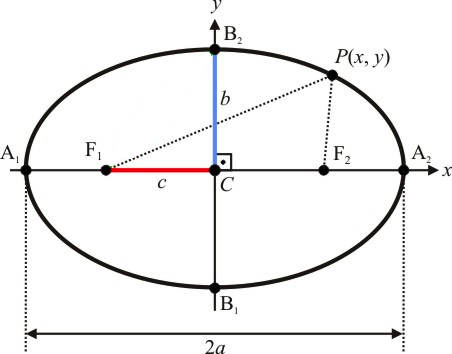
\includegraphics[width=0.5\textwidth]{./figures/problems/elipse.png}
\caption{Una elipse con algunos puntos
resaltados.\label{fig:prob:elipse}}
\end{figure}
\color{red}

\begin{enumerate}
\def\labelenumi{\arabic{enumi}.}
\tightlist
\item
  \textbf{Solución}
\end{enumerate}

\begin{quote}
\begin{enumerate}
\def\labelenumi{\alph{enumi})}
\tightlist
\item
  Dada la Figura 1, por simetría, se puede ver claramente que
  \(\overline{A_1F_1}=\overline{A_2F_2}\), por lo que la suma de las
  distancias de \(A_1\) a los focos sería
  \[\overline{A_1F_1}+\overline{A_1F_2}=\overline{A_2F_2}+\overline{A_1F_2}=2a.\]
\end{enumerate}
\end{quote}

\begin{quote}
\begin{quote}
Dado que, por definición, esa distancia es una costante para cualquier
punto, entonces esa constante debe ser igual a \(2a\).
\end{quote}
\end{quote}

\begin{quote}
\begin{enumerate}
\def\labelenumi{\alph{enumi})}
\setcounter{enumi}{1}
\tightlist
\item
  Si nos paramos, por ejemplo, en el punto \(B_2\), ya sabemos que
  \(\overline{F_1B_2}+\overline{B_2F_2}=2a\). Pero, por simetría,
  \(\overline{F_1B_2}=\overline{B_2F_2}=a\). Se hace claro, entonces,
  que \[a^2=b^2+c^2.\]
\end{enumerate}
\end{quote}

\begin{quote}
\begin{enumerate}
\def\labelenumi{\alph{enumi})}
\setcounter{enumi}{2}
\tightlist
\item
  Por definición, considerando el punto generalizado de la elipse
  \(P(x,y)\) medido desde \(C(0,0)\), tenemos
  \[\sqrt{\left(x+c\right)^{2}+y^{2}}+\sqrt{\left(x-c\right)^{2}+y^{2}}=2a.\]
\end{enumerate}
\end{quote}

\begin{quote}
\begin{quote}
Elevando al cuadrado:
\[\left(x+c\right)^{2}+y^{2}+\left(x-c\right)^{2}+y^{2}+2\sqrt{\left(x+c\right)^{2}+y^{2}}\sqrt{\left(x-c\right)^{2}+y^{2}}=4a^{2}.\]
Expandiendo y organizando:
\[\sqrt{\left(x+c\right)^{2}+y^{2}}\sqrt{\left(x-c\right)^{2}+y^{2}}=2a^{2}-x^{2}-c^{2}-y^{2}.\]
Elevando de nuevo al cuadrado:
\[\left(x^{2}+2cx+c^{2}+y^{2}\right)\left(x^{2}-2cx+c^{2}+y^{2}\right)=\left(2a^{2}-x^{2}-c^{2}-y^{2}\right)^{2}.\]
Expandiendo y sumando términos semejantes, se llega a
\[4a^{2}x^{2}+4a^{2}y^{2}-4c^{2}x^{2}=4a^{4}-4a^{2}c^{2}.\]
Factorizando, obtenemos
\[\left(a^{2}-c^{2}\right)x^{2}+a^{2}y^{2}=a^{2}(a^{2}-c^{2}).\] Por el
resultado del punto anterior, tenemos que \(a^{2}-c^{2}=b^{2}\), por lo
que tenemos \[b^{2}x^{2}+a^{2}y^{2}=a^{2}b^{2}.\] Dividiendo entre
\(a^{2}b^{2}\): \[\frac{x^{2}}{a^{2}}+\frac{y^{2}}{b^{2}}=1,\] que era a
lo que queríamos llegar.
\end{quote}
\end{quote}

\begin{quote}
\begin{enumerate}
\def\labelenumi{\alph{enumi})}
\setcounter{enumi}{3}
\tightlist
\item
  Dado que sabemos que \(a\), \(b\) y \(e\) se pueden relacionar
  mediante \(b=a\sqrt{1-e^2}\), podemos escribir el teorema de pitágoras
  como \textgreater{} \[a^{2}=a^{2}\left(1-e^{2}\right)+c^{2}.\]
  \textgreater{} Sumando términos semejantes, llegamos a que
  \textgreater{} \[e^{2}=\frac{c^{2}}{a^{2}}.\] \textgreater{} Debido a
  que \(a\), \(b\) y \(e\) se definien como reales positivos, obtenemos
  \textgreater{} \[e=\frac{c}{a},\] \textgreater{} que era lo que
  queríamos.
\end{enumerate}
\end{quote}

\begin{quote}
\begin{enumerate}
\def\labelenumi{\alph{enumi})}
\setcounter{enumi}{4}
\tightlist
\item
  El semilatus rectum hace parte de un triángulo rectángulo con \(F_1\)
  y \(F_2\) como los vértices de la base. Así, por la definición de
  todos los parámetros geométricos y de elipse como lugar geométrico,
  podemos escribir la relación \textgreater{}
  \[\left(2a-p\right)^{2}=\left(2c\right)^{2}+p^{2}.\] \textgreater{}
  Expandiendo, simplificando y despejando, obtenemos \textgreater{}
  \[p=\frac{a^{2}-c^{2}}{a}.\] \textgreater{} Pero como
  \(a^{2}-c^{2}=b^{2}\), entonces obtenemos \textgreater{}
  \[p=\frac{b^{2}}{a},\] \textgreater{} que era lo que queríamos.
\end{enumerate}
\end{quote}

\color{black}
\begin{enumerate}
\def\labelenumi{\arabic{enumi}.}
\setcounter{enumi}{1}
\tightlist
\item
  \textbf{Ecuación de una elipse}. Encuentre la ecuación general de la
  elipse cuyo semilatus rectum valga 9 y excentricidad sea 0.5.
\end{enumerate}
\color{red}

\begin{enumerate}
\def\labelenumi{\arabic{enumi}.}
\setcounter{enumi}{1}
\tightlist
\item
  \textbf{Solución}. Ya hemos demostrado que \(p=b^2/a\),
  \(b^2=a^2-c^2\) y \(c=ea\). Reemplazando la tercera en la segunda y
  ésta en la primera, se sigue
\end{enumerate}

\begin{quote}
\[9a=a^2-0.25a^2.\]
\end{quote}

\begin{quote}
Dado que \(a\neq 0,\) obtenemos \(a=12\), \(c=6\) y \(b=\sqrt{108}\).
Así, la ecuación ordinaria de la elipse sería
\end{quote}

\begin{quote}
\[\frac{x'^{2}}{144}+\frac{y'^{2}}{108}=1,\]
\end{quote}

\begin{quote}
que al multiplicar por 432 obtendríamos la ecuación general
\end{quote}

\begin{quote}
\[\boxed{3x'^2+4y'^2-432=0.}\]
\end{quote}

\color{black}
\begin{enumerate}
\def\labelenumi{\arabic{enumi}.}
\setcounter{enumi}{2}
\tightlist
\item
  \textbf{Parámetros geométricos}. Defina conceptualmente a qué
  corresponden cada uno de los siguientes parámetros en el caso de una
  elipse: a) defina \(F\), b) defina \(e\), c) defina \(p\), d) defina
  \(C\), e) defina \(a\), f) defina \(b\), g) defina \(r\), h) defina
  \(f\), i) defina \(E\).
\end{enumerate}
\color{red}

\begin{enumerate}
\def\labelenumi{\arabic{enumi}.}
\setcounter{enumi}{2}
\tightlist
\item
  \textbf{Solución}.
\end{enumerate}

\begin{quote}
\begin{enumerate}
\def\labelenumi{\alph{enumi})}
\tightlist
\item
  \(F\) corresponde a la distancia entre la directriz de la elipse y su
  foco. Es una distancia, pero no necesariamente es la
  \textit{distancia focal} (depende del sistema coordenado elegido). En
  el sistema coordenado ``natural'', coincide con la coordenada \(x\)
  del foco como punto del plano.
\end{enumerate}
\end{quote}

\begin{quote}
\begin{enumerate}
\def\labelenumi{\alph{enumi})}
\setcounter{enumi}{1}
\tightlist
\item
  \(e\) cooresponde a la excentricidad de la elipse, definida como la
  razón constante entre la distancia de cualquier punto de la elipse a
  su foco y la distancia de ese punto a la directriz. Indica qué tan
  achatada es la elipse. Entre más cercano sea \(e\) a 1, más achatada
  es la elipse. Entre más cercano a 0, más ``circular'' es.
\end{enumerate}
\end{quote}

\begin{quote}
\begin{enumerate}
\def\labelenumi{\alph{enumi})}
\setcounter{enumi}{2}
\tightlist
\item
  \(p\) corresponde al semilatus rectum de la elipse, la distancia entre
  su foco y un punto de la elipse sobre la perpendicular a su eje mayor
  que pasa por el foco.
\end{enumerate}
\end{quote}

\begin{quote}
\begin{enumerate}
\def\labelenumi{\alph{enumi})}
\setcounter{enumi}{3}
\tightlist
\item
  \(C\) corresponde al centro geométrico de la elipse. Puede
  considerarse una coordenada o una distancia. En el sistema coordenado
  «natural» corresponde a la coordenada \(x\) del centro de la elipse.
\end{enumerate}
\end{quote}

\color{black}\color{red}

\begin{quote}
\begin{enumerate}
\def\labelenumi{\alph{enumi})}
\setcounter{enumi}{4}
\tightlist
\item
  \(a\) corresponde al semieje mayor de la elipse. Es la distancia entre
  el centro geométrico de la elipse y uno de los puntos más alejados de
  éste.
\end{enumerate}
\end{quote}

\begin{quote}
\begin{enumerate}
\def\labelenumi{\alph{enumi})}
\setcounter{enumi}{5}
\tightlist
\item
  \(b\) corresponde al semieje menor de la elipse. Es la distancia entre
  el centro geométrico de la elipse y uno de los puntos más cercanos a
  éste.
\end{enumerate}
\end{quote}

\begin{quote}
\begin{enumerate}
\def\labelenumi{\alph{enumi})}
\setcounter{enumi}{6}
\tightlist
\item
  \(r\) corresponde a la coordenada radial en coordenadas polares de un
  punto de la elipse medido desde el foco de la misma.
\end{enumerate}
\end{quote}

\begin{quote}
\begin{enumerate}
\def\labelenumi{\alph{enumi})}
\setcounter{enumi}{7}
\tightlist
\item
  \(f\) corresponde a la coordenada angular en coordenadas polares
  (llamada anomalía verdadera) de un punto de la elipse medido desde el
  foco como polo y el eje mayor como eje polar.
\end{enumerate}
\end{quote}

\begin{quote}
\begin{enumerate}
\def\labelenumi{\roman{enumi})}
\tightlist
\item
  \(E\) corresponde a la anomalía excéntrica y es la coordenada angular
  de un punto de una circunferencia de radio \(a\) verticalmente
  superior al punto sobre la elipse con anomalía verdadera \(f\).
\end{enumerate}
\end{quote}

\color{black}
\begin{enumerate}
\def\labelenumi{\arabic{enumi}.}
\setcounter{enumi}{3}
\tightlist
\item
  \textbf{Traslación de las cónicas.} A partir de una completación de
  cuadrados, demuestre que la ecuación general de las cónicas sin
  términos acoplados
\end{enumerate}

\begin{quote}
\[Ax^2+Cy^2+Dx+Ey+G=0\]
\end{quote}

\begin{quote}
con \(A,C\neq 0\) se puede escribir, en su forma ordinaria, como
\end{quote}

\begin{quote}
\[\frac{x'^2}{q}+\frac{y'^2}{t}=1,\]
\end{quote}

\begin{quote}
donde \(x'\) y \(y'\) son las coordenadas de un punto en el sistema
trasladado dadas por
\end{quote}

\begin{quote}
\[x' = x+\frac{D}{2A},\] \[y' = y+\frac{E}{2C}\]
\end{quote}

\begin{quote}
y \(q,t\) están dadas por
\end{quote}

\begin{quote}
\[q   = -\frac{G}{A}+\frac{D^{2}}{4A^{2}}+\frac{E^{2}}{4AC},\]
\[t   = -\frac{G}{C}+\frac{D^{2}}{4AC}+\frac{E^{2}}{4C^{2}}.\]
\end{quote}

\begin{quote}
¿Qué condiciones se deben dar para que dicha cónica sea una
circunferencia, una elipse o una hipérbola? Dé un ejemplo numérico
sencillo de cada una.
\end{quote}
\color{red}

\begin{enumerate}
\def\labelenumi{\arabic{enumi}.}
\setcounter{enumi}{3}
\tightlist
\item
  \textbf{Solución}.
\end{enumerate}

\begin{quote}
Tomando la ecuación y sacando factor «común» \(A\) para los términos con
\(x\) y \(B\) para los términos con \(y\), se tiene
\end{quote}

\begin{quote}
\[A\left(x^{2}+\frac{D}{A}x\right)+C\left(y^{2}+\frac{E}{C}y\right)=-G.\]
\end{quote}

\begin{quote}
Sumando a ambos lados de la ecuación los términos \(D^{2}/4A\) y
\(E^{2}/4C\) convenientemente, se sigue que
\end{quote}

\begin{quote}
\[A\left(x^{2}+\frac{D}{A}x+\frac{D^{2}}{4A^{2}}\right)+C\left(y^{2}+\frac{E}{C}y+\frac{E^{2}}{4C^{2}}\right)=-G+\frac{D^{2}}{4A}+\frac{E^{2}}{4C}.\]
\end{quote}

\begin{quote}
Factorizando los trinomios cuadrado perfecto y dividiendo la ecuación
por todo el lado derecho, obtenemos
\end{quote}

\begin{quote}
\[\frac{\left(x+\frac{D}{2A}\right)^{2}}{-\frac{G}{A}+\frac{D^{2}}{4A^{2}}+\frac{E^{2}}{4AC}}+\frac{\left(y+\frac{E}{2C}\right)^{2}}{-\frac{G}{C}+\frac{C^{2}}{4AC}+\frac{E^{2}}{4C^{2}}}=1.\]
\end{quote}

\begin{quote}
Haciendo
\end{quote}

\begin{quote}
\[x' = x+\frac{D}{2A},\] \[y' = y+\frac{E}{2C},\]
\[q    = -\frac{G}{A}+\frac{D^{2}}{4A^{2}}+\frac{E^{2}}{4AC},\]
\[t    = -\frac{G}{C}+\frac{D^{2}}{4AC}+\frac{E^{2}}{4C^{2}},\]
\end{quote}

\begin{quote}
tenemos la ecuación de la cónica en su forma ordinaria pedida. Para que
esta cónica sea una circunferencia, debe suceder que \(q=t\) y que
\(q,t>0\); para que sea una elipse, debe suceder que \(q\neq t\) y que
\(q,t>0\); y para que sea una hipérbola, debe suceder que \(q>0\) y
\(t<0\) o viceversa. Nótese que \(t=\frac{C}{A}q\), lo que significa que
la ecuación pertenece a una circunferencia, también, cuando \(A=C\); a
una elipse cuando \(A\neq C\) pero \(A,C>0\); y a una hipérbola cuando
\(A>0\) y \(C<0\) o viceversa. Un ejemplo sencilla de cada una, en
orden, sería
\end{quote}

\begin{quote}
\[x'^{2}+y'^{2}=1,\qquad\frac{x'^{2}}{2}+y'^{2}=1,\qquad x'^{2}-y'^{2}=1.\]
\end{quote}

\color{black}
\begin{enumerate}
\def\labelenumi{\arabic{enumi}.}
\setcounter{enumi}{4}
\tightlist
\item
  \textbf{Rotación de cónicas.} A partir de la ecuación general de la
  cónica con términos acoplados
\end{enumerate}

\begin{quote}
\[Ax^2 + Bxy + Cy^2 + Dx + Ey + G = 0\]
\end{quote}

\begin{quote}
aplique una rotación de la forma
\end{quote}

\begin{quote}
\[x  =  x' \cos\theta - y' \sin\theta \]
\[y  =  x' \sin\theta + y' \cos\theta \]
\end{quote}

\begin{quote}
y demuestre que si se rota el sistema de coordenadas original un ángulo
\(\theta\) que satisface
\end{quote}

\begin{quote}
\[\tan 2\theta = \frac{B}{A-C},\]
\end{quote}

\begin{quote}
los nuevos ejes estarán alineados con los ejes de simetría.
\end{quote}
\color{red}

\begin{enumerate}
\def\labelenumi{\arabic{enumi}.}
\setcounter{enumi}{4}
\tightlist
\item
  \textbf{Solución}
\end{enumerate}

\begin{quote}
Al aplicar la rotación:
\end{quote}

\begin{quote}
\begin{eqnarray*}
A\left(x'\cos\theta-y'\sin\theta\right)^{2}+B\left(x'\cos\theta-y'\sin\theta\right)\left(x'\sin\theta+y'\cos\theta\right)+C\left(x'\sin\theta+y'\cos\theta\right)^{2}\\
+D\left(x'\cos\theta-y'\sin\theta\right)+E\left(x'\sin\theta+y'\cos\theta\right)+G=0.
\end{eqnarray*}
\end{quote}

\begin{quote}
Para que los nuevos ejes estén alineados con los ejes de simetría, es
necesario que los términos acoplados se anulen. Esto es, al expandir,
que suceda que
\end{quote}

\begin{quote}
\[-2Ax'y'\cos\theta\sin\theta+Bx'y'\cos^{2}\theta-Bx'y'\sin^{2}\theta+2Cx'y'\sin\theta\cos\theta=0.\]
\end{quote}

\begin{quote}
Dado que \(\cos^{2}\theta-\sin^{2}\theta=\cos 2\theta\) y
\(2\sin\theta\cos\theta=\sin 2\theta\), la condición se reduce a que
\end{quote}

\begin{quote}
\[-\sin2\theta\left(A-C\right)+B\cos2\theta=0\qquad\Longrightarrow\qquad\tan2\theta=\frac{B}{A-C},\]
\end{quote}

\begin{quote}
que era lo que queríamos demostrar.
\end{quote}

\color{black}
\begin{enumerate}
\def\labelenumi{\arabic{enumi}.}
\setcounter{enumi}{5}
\tightlist
\item
  \textbf{Órbitas de cometas.} El semieje mayor de un cometa es de 20 AU
  y la distancia entre el foco y el perihelio es de 1 AU.
\end{enumerate}

\begin{quote}
\begin{enumerate}
\def\labelenumi{\alph{enumi})}
\tightlist
\item
  ¿Cuál es la excentricidad de la órbita?
\end{enumerate}
\end{quote}

\begin{quote}
\begin{enumerate}
\def\labelenumi{\alph{enumi})}
\setcounter{enumi}{1}
\tightlist
\item
  ¿Cuánto vale el semieje menor?
\end{enumerate}
\end{quote}

\begin{quote}
\begin{enumerate}
\def\labelenumi{\alph{enumi})}
\setcounter{enumi}{2}
\tightlist
\item
  ¿Cuánto vale el semilatus rectum?
\end{enumerate}
\end{quote}

\begin{quote}
\begin{enumerate}
\def\labelenumi{\alph{enumi})}
\setcounter{enumi}{3}
\tightlist
\item
  Escriba la ecuación de este cometa en coordenadas polares.
\end{enumerate}
\end{quote}

\begin{quote}
\begin{enumerate}
\def\labelenumi{\alph{enumi})}
\setcounter{enumi}{4}
\tightlist
\item
  Haga un bosquejo de la situación medianamente a escala.
\end{enumerate}
\end{quote}
\color{red}

\begin{enumerate}
\def\labelenumi{\arabic{enumi}.}
\setcounter{enumi}{5}
\tightlist
\item
  \textbf{Solución}
\end{enumerate}

\begin{quote}
\begin{enumerate}
\def\labelenumi{\alph{enumi})}
\tightlist
\item
  Claramente, la distancia entre el foco y el perihelio debe ser
  \(r_1=a-c.\) Dado que \(r_1=1\) AU y que \(a=20\) AU, entonces
  \(c=19\) AU y, por lo tanto, \(\boxed{e=c/a=19/20=0.95}\).
\end{enumerate}
\end{quote}

\begin{quote}
\begin{enumerate}
\def\labelenumi{\alph{enumi})}
\setcounter{enumi}{1}
\tightlist
\item
  Dado que \(a^2=b^2+c^2\), entonces
  \(\boxed{b=\sqrt{39}=6.2\text{ AU}}\).
\end{enumerate}
\end{quote}

\begin{quote}
\begin{enumerate}
\def\labelenumi{\alph{enumi})}
\setcounter{enumi}{2}
\tightlist
\item
  Dado que \(p=b^2/a\), entonces \(\boxed{p=39/20=1.9\text{ AU}}\).
\end{enumerate}
\end{quote}

\begin{quote}
\begin{enumerate}
\def\labelenumi{\alph{enumi})}
\setcounter{enumi}{3}
\tightlist
\item
  La ecuación de la órbita de este cometa en coordenadas polares sería
  de la forma
  \[\boxed{r=\frac{39/20\mbox{ AU}}{1+\frac{19}{20}\cos f}=\frac{1.9\mbox{ AU}}{1+0.95\cos f}}\]
\end{enumerate}
\end{quote}

\color{black}
\begin{enumerate}
\def\labelenumi{\arabic{enumi}.}
\setcounter{enumi}{6}
\tightlist
\item
  \textbf{Órbita lunar.} Sobre una órbita lunar, el punto más cercano al
  satélite se conoce como periselenio y el más lejano como aposelenio.
  La nave Apolo 11 fue puesta en una órbita elíptica alrededor de la
  luna con una altitud (respecto a la superficie lunar) en el
  periselenio de 110 km y de 314 km en el aposelenio. Encuentre la
  ecuación de esta elipse en coordenadas polares si el radio de la luna
  es de 1728 km y el centro de la luna se encuentra en uno de los focos
  de la elipse. Haga un bosquejo de la situación medianamente a escala.
\end{enumerate}
\color{red}

\begin{enumerate}
\def\labelenumi{\arabic{enumi}.}
\setcounter{enumi}{6}
\tightlist
\item
  \textbf{Solución}
\end{enumerate}

\begin{quote}
En primer lugar, sabemos que la distancia entre el periselenio y el
aposelenio debe ser 2 veces el semieje mayor de la órbita del satélite.
Así
\end{quote}

\begin{quote}
\[a=\frac{110+2\times 1728+314}{2} \mbox{ km}=1940\mbox{ km}.\]
\end{quote}

\begin{quote}
Además, la distancia entre el centro de la luna (foco) y el periselenio
es, como ya se había dicho, \(a-c=1728\mbox{ km}+110\mbox{ km}\), por lo
que \(c=102\mbox{ km}\). Así, \(e=c/a=0.053\),
\(b^2=a^2-c^2=3753196\mbox{ km}^\text{o}\) y \(p=b^2/a=1935\) km. Y, por
lo tanto, la ecuación de esta elipse en coordenadas polares sería
\end{quote}

\begin{quote}
\[\boxed{r=\frac{1935\mbox{ km}}{1+0.053\cos f}.}\]
\end{quote}

\color{black}
\begin{enumerate}
\def\labelenumi{\arabic{enumi}.}
\setcounter{enumi}{7}
\tightlist
\item
  \textbf{Anomalías.}
\end{enumerate}

\begin{quote}
\begin{enumerate}
\def\labelenumi{\alph{enumi})}
\tightlist
\item
  Demuestre que, para una elipse, la distancia radial, \(r\), está
  relacionada con la anomalía excéntrica, \(E\), por medio de la
  expresión
\end{enumerate}
\end{quote}

\begin{quote}
\[
r=a(1 - e\cos E).
\]
\end{quote}

\begin{quote}
\begin{enumerate}
\def\labelenumi{\alph{enumi})}
\setcounter{enumi}{1}
\tightlist
\item
  Demuestre, además, que la anomalía verdadera se relaciona con la
  anomalía excéntrica a través de
\end{enumerate}
\end{quote}

\begin{quote}
\[
\tan \frac{f}{2} = \sqrt{\frac{1+e}{1-e}}\tan \frac{E}{2}.
\]
\end{quote}
\color{red}

\begin{enumerate}
\def\labelenumi{\arabic{enumi}.}
\setcounter{enumi}{7}
\tightlist
\item
  \textbf{Solución}
\end{enumerate}

\begin{quote}
\begin{enumerate}
\def\labelenumi{\alph{enumi})}
\tightlist
\item
  Si definimos la elipse como el lugar geométrico de los puntos tal que
  están a una distancia del eje \(x\) en proporción \(b/a\) de la
  distancia de los puntos de una circunferencia de radio \(a\) que se
  muestra en la Figura \ref{anomalia-excentrica}, entonces
\end{enumerate}
\end{quote}

\begin{quote}
\[\frac{\overline{PD}}{\overline{QD}} = \frac{b}{a}\]
\end{quote}

\begin{quote}
Si usamos el teorema de Pitágoras para relacionar \(r\) con los
distintos segmentos de la figura obtenemos \[
r^2 = (\overline{DF})^2 + (\overline{PD})^2 = (\overline{CF}-\overline{CD})^2 + \left(\frac{b}{a}\overline{QD}\right)^2
\]
\end{quote}

\begin{quote}
Por la geometría de la elipse sabemos sin embargo que
\(\overline{CD}=a\cos E\), \(\overline{QD}=a\sin E\) y que la distancia
focal \(\overline{CF}=ea\). Así,
\end{quote}

\begin{quote}
\begin{eqnarray*}
r^{2}&=&(ea-a\cos E)^{2}+\left(\frac{b}{a}a\sin E\right)^{2}\\\mbox{expandiendo }\rightarrow&=&e^{2}a^{2}-2ea^{2}\cos E+a^{2}\cos^{2}E+b^{2}\sin^{2}E\\\sin^{2}E=1-\cos^{2}E\rightarrow&=&e^{2}a^{2}-2ea^{2}\cos E+a^{2}\cos^{2}E+b^{2}-b^{2}\cos^{2}E\\\mbox{agrupando }\rightarrow&=&\left(e^{2}a^{2}+b^{2}\right)-2ea^{2}\cos E+\left(a^{2}-b^{2}\right)\cos^{2}E\\c=e/a\mbox{ y }a^{2}=b^{2}+c^{2}\rightarrow&=&a^{2}-2ea^{2}\cos E+e^{2}a^{2}\cos^{2}E\\\mbox{factorizando }\rightarrow&=&a^{2}\left(1-e\cos E\right)^{2}\\r&=&a\left(1-e\cos E\right).
\end{eqnarray*}
\end{quote}

\begin{quote}
\begin{enumerate}
\def\labelenumi{\alph{enumi})}
\setcounter{enumi}{1}
\tightlist
\item
  Primero, nótese que para cualquier ángulo \(\theta\) se satisface la
  identidad
\end{enumerate}
\end{quote}

\begin{quote}
\[\tan\left(\frac{\theta}{2}\right)=\frac{\sin(\theta/2)}{\cos(\theta/2)}=\frac{\sqrt{\frac{1-\cos\theta}{2}}}{\sqrt{\frac{1+\cos\theta}{2}}}=\sqrt{\frac{1-\cos\theta}{1+\cos\theta}\times1}=\sqrt{\frac{1-\cos\theta}{1+\cos\theta}\times\frac{1+\cos\theta}{1+\cos\theta}}=\sqrt{\frac{1-\cos^{2}\theta}{\left(1+\cos\theta\right)^{2}}}=\sqrt{\frac{\sin^{2}\theta}{\left(1+\cos\theta\right)^{2}}}=\frac{\sin\theta}{1+\cos\theta},\]
\end{quote}

\begin{quote}
por lo que, entonces,
\end{quote}

\begin{quote}
\[\tan\frac{f}{2}=\frac{\sin f}{1+\cos f}.\]
\end{quote}

\begin{quote}
Se puede ver que \(\sin{f}=\overline{PD}/r\) y que
\(\cos{f}=(a\cos{E}-ae)/r\), por lo que
\end{quote}

\begin{quote}
\[\tan\frac{f}{2}=\frac{\overline{PD}}{r+a\cos E-ae}.\]
\end{quote}

\begin{quote}
Debido a que tenemos que \(\overline{PD}=b\sin E\),
\(r=a\left(1-e\cos E\right)\) y que \(b=a\sqrt{1-e^{2}}\), entonces,
factorizando y racionalizando, se obtiene
\end{quote}

\begin{quote}
\[\tan\frac{f}{2}=\sqrt{\frac{1+e}{1-e}}\frac{\sin E}{1+\cos E}.\]
\end{quote}

\begin{quote}
Pero como \[\frac{\sin E}{1+\cos E}=\tan\frac{E}{2},\] entonces
\[\tan\frac{f}{2}=\sqrt{\frac{1+e}{1-e}}\tan\frac{E}{2}.\]
\end{quote}

\color{black}
\begin{enumerate}
\def\labelenumi{\arabic{enumi}.}
\setcounter{enumi}{8}
\tightlist
\item
  \textbf{Parámetros de elipse}. Dada la ecuación de la elipse
  \(x^2 + 2y^2 + 2x + y - 6 = 0\) complete cuadrados y llévela a su
  forma ordinaria, para determina la posición del centro, el semieje
  mayor, semieje menor, distancia focal y semilatus rectum.
\end{enumerate}
\color{red}

\begin{enumerate}
\def\labelenumi{\arabic{enumi}.}
\setcounter{enumi}{8}
\tightlist
\item
  \textbf{Solución}
\end{enumerate}

\begin{quote}
Agrupemos las \(x\) y las \(y\):
\end{quote}

\begin{quote}
\[\left(x^{2}+2x\right)+2\left(y^{2}+\frac{y}{2}\right)=6.\]
\end{quote}

\begin{quote}
Completemos cuadrados:
\end{quote}

\begin{quote}
\[\left(x^{2}+2x+1\right)+2\left(y^{2}+\frac{y}{2}+\frac{1}{16}\right)=6+1+\frac{1}{8}.\]
\end{quote}

\begin{quote}
Factoricemos y dividamos ambos lados entre 57/8:
\end{quote}

\begin{quote}
\[\boxed{\frac{\left(x+1\right)^{2}}{57/8}+\frac{\left(y+\frac{1}{4}\right)^{2}}{57/16}=1.}\]
\end{quote}

\begin{quote}
Tenemos, entonces, que el centro de la elipse es el punto
\(\boxed{C(-1,-1/4)}\), los semiejes mayor y menores son
\(\boxed{a=\sqrt{57/8}=2.7}\) y \(\boxed{b=\sqrt{57/16}=1.9}\), la
distancia focal es \(\boxed{c=\sqrt[]{a^2-b^2}=b}\) y el semilatus
rectum es \(\boxed{p=b^2/a=1.3}\). Grafiquemos:
\end{quote}

\color{black}
\begin{enumerate}
\def\labelenumi{\arabic{enumi}.}
\setcounter{enumi}{9}
\tightlist
\item
  \textbf{Elementos orbitales.} Para un satélite en órbita alrededor de
  la Tierra se tienen los siguientes elementos orbitales:
  \(a=8016.0\mbox{ km}\), \(e=0.06\), \(I=50^\text{o}\),
  \(\Omega=0.0^\text{o}\), \(\omega=30^\text{o}\) y \(f=20^\text{o}\).
  Encuentre el vector de posición en el plano fundamental del ecuador
  terrestre.
\end{enumerate}
\color{red}

\begin{enumerate}
\def\labelenumi{\arabic{enumi}.}
\setcounter{enumi}{9}
\tightlist
\item
  \textbf{Solución}
\end{enumerate}

\begin{quote}
Es claro que, en el plano de la órbita del satélite, se satisface
\(z'''=0\) y que
\[r=\frac{a\left(1-e^{2}\right)}{1+e\cos f}\qquad\Longrightarrow\qquad x'''=r\cos f\quad\mbox{y}\quad y'''=r\sin f.\]
\end{quote}

\color{black}
    \begin{code}{}{}\begin{Verbatim}[fontsize=\small,commandchars=\\\{\}]
\PY{k+kn}{import} \PY{n+nn}{numpy} \PY{k}{as} \PY{n+nn}{np}
\PY{n}{GRADOS}\PY{o}{=}\PY{n}{np}\PY{o}{.}\PY{n}{pi}\PY{o}{/}\PY{l+m+mi}{180}
\PY{n}{a} \PY{o}{=} \PY{l+m+mf}{8016.}
\PY{n}{e} \PY{o}{=} \PY{l+m+mf}{0.06}
\PY{n}{f} \PY{o}{=} \PY{l+m+mi}{20}\PY{o}{*}\PY{n}{GRADOS}

\PY{n}{r} \PY{o}{=} \PY{n}{a}\PY{o}{*}\PY{p}{(}\PY{l+m+mi}{1}\PY{o}{\PYZhy{}}\PY{n}{e}\PY{o}{*}\PY{n}{e}\PY{p}{)}\PY{o}{/}\PY{p}{(}\PY{l+m+mi}{1}\PY{o}{+}\PY{n}{e}\PY{o}{*}\PY{n}{np}\PY{o}{.}\PY{n}{cos}\PY{p}{(}\PY{n}{f}\PY{p}{)}\PY{p}{)}
\PY{n}{xppp} \PY{o}{=} \PY{n}{r}\PY{o}{*}\PY{n}{np}\PY{o}{.}\PY{n}{cos}\PY{p}{(}\PY{n}{f}\PY{p}{)}
\PY{n}{yppp} \PY{o}{=} \PY{n}{r}\PY{o}{*}\PY{n}{np}\PY{o}{.}\PY{n}{sin}\PY{p}{(}\PY{n}{f}\PY{p}{)}
\PY{n}{zppp} \PY{o}{=} \PY{l+m+mi}{0}
\PY{n}{rppp}\PY{o}{=}\PY{n}{np}\PY{o}{.}\PY{n}{array}\PY{p}{(}\PY{p}{[}\PY{p}{[}\PY{n}{xppp}\PY{p}{]}\PY{p}{,} \PY{p}{[}\PY{n}{yppp}\PY{p}{]}\PY{p}{,} \PY{p}{[}\PY{n}{zppp}\PY{p}{]}\PY{p}{]}\PY{p}{)}
\PY{n+nb}{print}\PY{p}{(}\PY{l+s+s1}{\PYZsq{}}\PY{l+s+s1}{El vector posición en el plano orbital es, en km,}\PY{l+s+se}{\PYZbs{}n}\PY{l+s+s1}{\PYZsq{}}\PY{p}{,}\PY{n}{rppp}\PY{p}{)}
\end{Verbatim}

%%

\end{code}

    \begin{Verbatim}[fontsize=\small,commandchars=\\\{\}]
El vector posición en el plano orbital es, en km,
 [[7104.87486548]
 [2585.96296922]
 [   0.        ]]
\end{Verbatim}
\color{red}

\begin{quote}
Recordemos que \texttt{SPICE} tiene una rutina predefinida para calcular
una matriz de rotación a partir de tres ángulos de Euler:
\texttt{eul2m}. Usándo la matriz para pasar del sistema no primado al
primado quedaría:
\end{quote}

\color{black}
    \begin{code}{}{}\begin{Verbatim}[fontsize=\small,commandchars=\\\{\}]
\PY{k+kn}{import} \PY{n+nn}{spiceypy} \PY{k}{as} \PY{n+nn}{spy}
\PY{n}{i} \PY{o}{=} \PY{l+m+mi}{50}\PY{o}{*}\PY{n}{GRADOS}
\PY{n}{Omega} \PY{o}{=} \PY{l+m+mi}{0}\PY{o}{*}\PY{n}{GRADOS}
\PY{n}{omega} \PY{o}{=} \PY{l+m+mi}{30}\PY{o}{*}\PY{n}{GRADOS}

\PY{n}{R3d}\PY{o}{=}\PY{n}{spy}\PY{o}{.}\PY{n}{eul2m}\PY{p}{(}\PY{n}{omega}\PY{p}{,}\PY{n}{i}\PY{p}{,}\PY{n}{Omega}\PY{p}{,}\PY{l+m+mi}{3}\PY{p}{,}\PY{l+m+mi}{1}\PY{p}{,}\PY{l+m+mi}{3}\PY{p}{)}
\PY{n}{R3d}
\end{Verbatim}

%%

\end{code}

\begin{Verbatim}[fontsize=\small,commandchars=\\\{\}]
{\color{outcolor}Out[{\color{outcolor}81}]:} array([[ 0.8660254 ,  0.3213938 ,  0.38302222],
                [-0.5       ,  0.5566704 ,  0.66341395],
                [ 0.        , -0.76604444,  0.64278761]])
\end{Verbatim}
            \color{red}

Pero queremos pasar del sistema primado al no primado, entonces sacamos
la inversa (o traspuesta, que es lo mismo para matrices de rotación):

\color{black}
    \begin{code}{}{}\begin{Verbatim}[fontsize=\small,commandchars=\\\{\}]
\PY{n}{R3D} \PY{o}{=} \PY{n}{np}\PY{o}{.}\PY{n}{transpose}\PY{p}{(}\PY{n}{R3d}\PY{p}{)} 
\PY{n}{R3D}
\end{Verbatim}

%%

\end{code}

\begin{Verbatim}[fontsize=\small,commandchars=\\\{\}]
{\color{outcolor}Out[{\color{outcolor}82}]:} array([[ 0.8660254 , -0.5       ,  0.        ],
                [ 0.3213938 ,  0.5566704 , -0.76604444],
                [ 0.38302222,  0.66341395,  0.64278761]])
\end{Verbatim}
            \color{red}

Así, el vector posición está dado por

\color{black}
    \begin{code}{}{}\begin{Verbatim}[fontsize=\small,commandchars=\\\{\}]
\PY{n}{R3D}\PY{o}{.}\PY{n}{dot}\PY{p}{(}\PY{n}{rppp}\PY{p}{)}
\end{Verbatim}

%%

\end{code}

\begin{Verbatim}[fontsize=\small,commandchars=\\\{\}]
{\color{outcolor}Out[{\color{outcolor}83}]:} array([[4860.02063961],
                [3722.99180441],
                [4436.88885811]])
\end{Verbatim}
            
\begin{enumerate}
\def\labelenumi{\arabic{enumi}.}
\setcounter{enumi}{10}
\tightlist
\item
  \textbf{Circunferencia máxima.} La posición de un punto sobre la
  Tierra se especifica por su longitud \(\phi\) y latitud \(\lambda\),
  como se muestra en la \autoref{fig:prob:latlon}.
\end{enumerate}

\begin{quote}
Sean los vectores desde el centro de la Tierra hacia dos puntos
\(\vec{r}_{1}\) y \(\vec{r}_{2}\). El coseno del ángulo \(\theta\) entre
ellos puede ser hallado a partir de su producto escalar (producto
punto), de tal manera que la distancia a lo largo del círculo máximo
entre los dos puntos es \(R\theta\).
\end{quote}

\begin{quote}
Encuentre una expresión para \(\theta\) en términos de las coordenadas
de los dos puntos.
\end{quote}

\begin{figure}[t!]
\centering
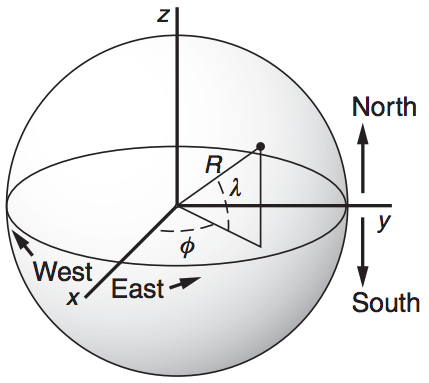
\includegraphics[width=0.5\textwidth]{./figures/problems/earth.png}
\caption{Definición de elas coordenadas de latitud y longitud sobre la
Tierra\label{fig:prob:latlon}}
\end{figure}
\color{red}

\begin{enumerate}
\def\labelenumi{\arabic{enumi}.}
\setcounter{enumi}{10}
\tightlist
\item
  \textbf{Solución}
\end{enumerate}

\begin{quote}
El vector posición \(\vec{r}_i\) sobre la superficie de la Tierra tendrá
coordenadas cartesianas \(x_i=R\cos\lambda_i\cos\phi_i\),
\(y_i=R\cos\lambda_i\sin\phi_i\) y \(z_i=R\sin\lambda_i\). Así, el
producto punto entre \(\vec{r}_1\) y \(\vec{r}_2\) se puede calcular
como \(R^2\cos\theta\) y, a la vez, como la suma de los productos de las
componentes \(x_1x_2+y_1y_2+z_1z_2\), de tal forma que
\end{quote}

\begin{quote}
\[R^2\cos\theta=R^2(\cos\lambda_1\cos\phi_1\cos\lambda_2\cos\phi_2+\cos\lambda_1\sin\phi_1\cos\lambda_2\sin\phi_2+\sin\lambda_1\sin\lambda_2).\]
\end{quote}

\begin{quote}
Sacando factor común \(\cos\lambda_1\cos\lambda_2\) en los primeros dos
términos y teniendo en cuenta la identidad
\(\cos\phi_1\cos\phi_2+\sin\phi_1\sin\phi_2=\cos(\phi_1-\phi_2)\),
obtenemos la expresión para \(\theta\) pedida:
\end{quote}

\begin{quote}
\[\boxed{\theta=\arccos(\cos\lambda_1\cos\lambda_2\cos(\phi_1-\phi_2)+\sin\lambda_1\sin\lambda_2)}\]
\end{quote}

\color{black}
\begin{enumerate}
\def\labelenumi{\arabic{enumi}.}
\setcounter{enumi}{11}
\tightlist
\item
  \textbf{Derivada temporal de los vectores unitarios.} La figura
  muestra la configuración de un sistema de coordenadas polares definido
  por (\(\hat{r},\hat{\theta}\)) relativo a un sistema cartesiano. Los
  conjuntos de vectores (\(\hat{r},\hat{\theta}\)) y
  (\(\hat{i},\hat{j}\)) son constantes en magnitud pero solamente los
  vectores cartesianos lo son también en dirección. Conforme la
  partícula de vector posición \(\vec{r}\) se desplaza, los vectores
  (\(\hat{r},\hat{\theta}\)) cambian de dirección, de forma tal que es
  posible definir una derivada temporal de estos.
\end{enumerate}

\begin{quote}
\begin{enumerate}
\def\labelenumi{\alph{enumi})}
\tightlist
\item
  Muestre que
\end{enumerate}
\end{quote}

\begin{quote}
\[
\frac{d\hat{r}}{dt} = \dot{\theta}\hat{\theta}
\]
\end{quote}

\begin{quote}
\[
\frac{d\hat{\theta}}{dt} = -\dot{\theta}\hat{r}
\]
\end{quote}

\begin{quote}
\begin{enumerate}
\def\labelenumi{\alph{enumi})}
\setcounter{enumi}{1}
\tightlist
\item
  Usando los resultados del punto anterior, muestre que el vector
  aceleración en coordenadas polares viene dado por
\end{enumerate}
\end{quote}

\begin{quote}
\[
\vec{a}=(\ddot{r}-r\dot{\theta}^2)\hat{r} + (r\ddot{\theta}+2\dot{r}\dot{\theta})\hat{\theta}
\]
\end{quote}
\color{red}

\begin{enumerate}
\def\labelenumi{\arabic{enumi}.}
\setcounter{enumi}{11}
\tightlist
\item
  \textbf{Solución}
\end{enumerate}

\begin{quote}
En primer lugar, se puede ver claramente de la figura dada que el vector
unitario \(\hat{r}\) se puede escribir como una suma de \(\cos\theta\)
en \(\hat{i}\) y de \(\sin\theta\) en \(\hat{j}\), al igual que el
vector unitario \(\hat{\theta}\) se puede escribir como una suma de
\(-\sin\theta\) en \(\hat{i}\) y de \(\cos\theta\) en \(\hat{j}\).
\end{quote}

\begin{quote}
\begin{enumerate}
\def\labelenumi{\alph{enumi}.}
\tightlist
\item
  Así,
\end{enumerate}
\end{quote}

\begin{quote}
\begin{quote}
\[\frac{\mathrm{d}\hat{r}}{\mathrm{d}t}=\frac{\mathrm{d}}{\mathrm{d}t}(\cos\theta \hat{i}+\sin\theta\hat{j})\]
\end{quote}
\end{quote}

\begin{quote}
\begin{quote}
Pero como \(\mathrm{d}(\sin\theta)/\mathrm{d}t=\dot{\theta}\cos\theta\),
\(\mathrm{d}(\cos\theta)/\mathrm{d}t=-\dot{\theta}\sin\theta\) y los
vecotres unitarios \(\hat{i}\) y \(\hat{j}\) no cambian en el tiempo,
entonces
\[\frac{\mathrm{d}\hat{r}}{\mathrm{d}t}=-\dot{\theta}\sin\theta \hat{i}+\dot{\theta}\cos\theta\hat{j}=\dot{\theta}\hat{\theta}\]
\end{quote}
\end{quote}

\begin{quote}
\begin{quote}
De igual forma,
\end{quote}
\end{quote}

\begin{quote}
\begin{quote}
\[\frac{\mathrm{d}\hat{\theta}}{\mathrm{d}t}=\frac{\mathrm{d}}{\mathrm{d}t}(-\sin\theta \hat{i}+\cos\theta\hat{j})=-\dot{\theta}\cos\theta \hat{i}-\dot{\theta}\sin\theta\hat{j}=-\dot{\theta}\hat{r}\]
\end{quote}
\end{quote}

\begin{quote}
\begin{enumerate}
\def\labelenumi{\alph{enumi}.}
\setcounter{enumi}{1}
\tightlist
\item
  Dado que \(\vec{r}=r\hat{r}\), entonces
\end{enumerate}
\end{quote}

\begin{quote}
\begin{quote}
\[\dot{\vec{r}}=\dot{r}\hat{r}+r\frac{\mathrm{d}\hat{r}}{\mathrm{d}t}=\dot{r}\hat{r}+r\dot{\theta}\hat{\theta}\]
\end{quote}
\end{quote}

\begin{quote}
\begin{quote}
Y por lo tanto
\end{quote}
\end{quote}

\begin{quote}
\begin{quote}
\[\ddot{\vec{r}}=\ddot{r}\hat{r}+\dot{r}\dot{\theta}\hat{\theta}+\dot{r}\dot{\theta}\hat{\theta}+r\ddot{\theta}\hat{\theta}-r\dot{\theta}^2\hat{r}\]
\end{quote}
\end{quote}

\begin{quote}
\begin{quote}
Agrupando,
\end{quote}
\end{quote}

\begin{quote}
\begin{quote}
\[\ddot{\vec{r}}=(\ddot{r}-r\dot{\theta}^2)\hat{r}+(2\dot{r}\dot{\theta}+r\ddot{\theta})\hat{\theta}\]
\end{quote}
\end{quote}

\begin{quote}
\begin{enumerate}
\def\labelenumi{\alph{enumi}.}
\setcounter{enumi}{2}
\tightlist
\item
  Volviendo a derivar:
\end{enumerate}
\end{quote}

\begin{quote}
\begin{quote}
\[\dddot{\vec{r}}=\dddot{r}\hat{r}+\ddot{r}\dot{\theta}\hat{\theta}+2\ddot{r}\dot{\theta}\hat{\theta}+2\dot{r}\ddot{\theta}\hat{\theta}-2\dot{r}\dot{\theta}^2\hat{r}+\dot{r}\ddot{\theta}\hat{\theta}+r\dddot{\theta}\hat{\theta}-r\ddot{\theta}\dot{\theta}\hat{r}-\dot{r}\dot{\theta}^2\hat{r}-2r\dot{\theta}\ddot{\theta}\hat{r}-r\dot{\theta}^3\hat{\theta}\]
\end{quote}
\end{quote}

\begin{quote}
\begin{quote}
Agrupando,
\[\dddot{\vec{r}}=(\dddot{r}-3\dot{r}\dot{\theta}^2-3r\dot{\theta}\ddot{\theta})\hat{r}+(3\ddot{r}\dot{\theta}+3\dot{r}\ddot{\theta}+r\dddot{\theta}-r\dot{\theta}^3)\hat{\theta}\]
En el caso de una partícula moviéndose en una circunferencia de radio
\(R\) (\(r=R\), \(\dot{r}=\ddot{r}=\dddot{r}=0\)) con rapidez angular
\(\omega\) (\(\dot{\theta}=\omega\),
\(\ddot{\theta}=\dddot{\theta}=0\)), el tirón sería
\[\dddot{\vec{r}}=-R\omega^3\hat{\theta}\]
\end{quote}
\end{quote}

\color{black}
\hypertarget{mecanica}{%
\chapter{Mecánica newtoniana}\label{mecanica}}
\label{sec:04-5_Mecanica}\begin{box_summary}{Resumen}

En este capítulo presentaremos una síntesis moderna de los mecánica
newtoniana, aplicada específicamente a partículas (puntuales). Sobre la
base de los principios, postulados y proposiciones de la mecánica
newtoniana formularemos los principales resultados de la mecánica
celeste que desarrollamos en este libro. Daremos un especial énfasis a
la mecánica de sistemas de partículas interactuantes, descritos tanto en
sistemas de referencia inerciales como no inerciales. En este último
caso nos concentraremos en en los sistemas de referencia rotante, que
son importantes para la descripción del problema restringido de los tres
cuerpos que estudiaremos más adelante.

\end{box_summary}


\hypertarget{mecanica_introduccion}{%
\section{Introducción}\label{mecanica_introduccion}}

Conocemos con el nombre de \textbf{mecánica} al conjunto de
definiciones, principios y leyes físicas que permiten describir el
movimiento de los cuerpos materiales (cinemática) y la relación con los
agentes que los producen y perturban (dinámica).

La mecánica se ha desarrollado históricamente durante dos períodos. El
primero período esta comprendido entre la publicación de los
\emph{hilosophiae Naturalis Principia Mathematica} por Sir Isaac Newton
\cite{Newton1780Principia} y los artículos fundamentales de la teoría de
la relatividad de 1905. A la mecánica de este período la llamaremos
\textbf{mecánica prerrelativistica} o \textbf{mecánica newtoniana}. El
segundo período cubre el tiempo entre 1905 y el presente. A la mecánica
que se desarrollo después de los trabajos originales de Einstein la
llamaremos \textbf{mecánica relativística} e incluye las teorías
especial (mecánica en espacio-tiempo plano) y general de la relatividad
(gravitación moderna.)

El adjetivo newtoniano, que usaremos a lo largo de este capítulo, no
significa que las cantidades, principios y leyes que formularemos aquí
fueron todas inventadas por Newton. Por un lado, además de sus ideas
originales, Newton también compiló y sistematizo ideas que ya existían
en su época; por el otro, mucha de sus ideas fueron también ampliadas
durante casi 200 años después de la publicación de sus obras.

Lo \emph{newtoniano} se refiere aquí al hecho de que en la definición de
las cantidades básicas y en la formulación de las leyes, asumiremos,
como lo hizo Newton en los \emph{Principia} y lo hicieron sus sucesores
hasta principios de los 1900, que: (1) el espacio y el tiempo son
entidades independientes y no son afectadas por la materia y (2) la
gravedad es una fuerza de acción instantánea a distancia.

Aunque hoy nos parezca increíble, casi toda la mecánica celeste de los
últimos 350 años se ha formulado sobre la base de estos principios que
hoy sabemos no describen la realidad fundamental del Universo.

La mecánica es una teoría muy amplia que se usa para describir no solo
el movimiento de cuerpos o partículas individuales, sino también el
movimiento, rotación y deformación de cuerpos materiales continuos
(cuerpos rígidos y fluídos.) En este capítulo (y en lo que resta del
libro) nos concentraremos, sin embargo, en la mecánica de partículas o
sistemas de partículas (nubes de partículas que interactúan debilmente y
a distancia entre ellas.)

Antes de proceder a formular los principios (axiomas) y postulados
(leyes) en los que se fundamenta la mecánica newtoniana, es necesario
definir primero, las cantidades físicas que requerimos en esta tarea.
Definir estas cantidades en todo rigor, no solo es un ejercicio
intelectual indispensable en la formulación de una teoría, sino, como
veremos, puede ser la fuente misma de algunas ideas claves.



\hypertarget{cinematica}{%
\section{Cinemática}\label{cinematica}}

\hypertarget{cantidades_cinematicas}{%
\subsection{Cantidades cinemáticas}\label{cantidades_cinematicas}}

Las cantidades cinemáticas son aquellas que se usan para describir el
movimiento, tal y como ocurre, independiente de sus causas.

Para detalles sobre las convenciones y la notación de las cantidades
definidas abajo se recomienda leer la
\autoref{conjuntos_tuplas_vectores},
\autoref{sistemas_coordenadas} y \autoref{derivadas}.

\begin{itemize}
\item
  \textbf{Tiempo}, \(t\): Un número real que indica el \emph{intervalo}
  transcurrido desde un \emph{instante} de referencia. Esta cantidad es
  \emph{independiente y absoluta} (ver comentarios abajo.)
\item
  \textbf{Posición (o vector posición), \(\vec r\)}: Es el vector que va
  del origen de coordenadas a un lugar del espacio.

  \begin{itemize}
  \tightlist
  \item
    Coordenadas cartesianas:
    \(\vec r= x\hat{e}_x+y\hat{e}_y+z\hat{e}_z\).
  \item
    Coordenadas cilíndricas: \(\vec r= r\hat{e}_r+z\hat{e}_z\).
  \item
    Coordenadas esféricas: \(\vec r= r\hat{e}_r\).
  \end{itemize}
\end{itemize}

\begin{itemize}
\tightlist
\item
  \textbf{Velocidad \(\vec v\)}:

  \begin{itemize}
  \tightlist
  \item
    Definición general:
    \(\vec v\equiv \mathrm{d}\vec r/\mathrm{d}t=\dot{\vec r}\).
  \item
    Coordenadas cartesianas:
    \(\vec v=\dot{x}\hat{e}_x+\dot{y}\hat{e}_y+\dot{z}\hat{e}_z\).
  \item
    Coordenadas cilíndricas:
    \(\vec v=\dot{r}\hat{e}_r+r\dot{\theta}\hat{e}_\theta+\dot{z}\hat{e}_z\).
  \item
    Coordenadas esféricas:
    \(\vec v=\dot{r} \hat{e}_r + r\dot\theta\cos\phi \hat{e}_\theta + r\dot\phi \hat{e}_\phi\)
  \end{itemize}
\end{itemize}

\begin{itemize}
\item
  \textbf{Estado \(\vec X\)}: En el contexto de la cinemática en
  mecánica celeste, llamamos vector de estado \(\vec X\), al vector
  formado por la unión de las componentes cartesianas de los vectores
  posición y velocidad, \(\vec{X}:(x,y,z,\dot x,\dot y,\dot z)\). En
  distintos contextos será más conveniente denotar al vector de estado
  usando \emph{notación matricial}, como un vector columna (matriz
  \(6\times1\)) \(\vec X:(x\;y\;z\;\dot x\;\dot y\;\dot z)^\mathrm{T}\)
  o explícitamente:

  \begin{equation}
    \vec X:\left(
    \begin{array}{c}
    x \\ y \\ z \\ \dot x\\ \dot y\\ \dot z
    \end{array}
    \right)
    \end{equation}
\end{itemize}

\begin{itemize}
\tightlist
\item
  \textbf{Aceleración \(\vec a\)}:

  \begin{itemize}
  \tightlist
  \item
    Definición general:
    \(\vec a \equiv \mathrm{d}\vec v/\mathrm{d}t=\dot{\vec v}=\mathrm{d}^2\vec r/\mathrm{d}t^2=\ddot{\vec{r}}\).
  \item
    Coordenadas cartesianas:
    \(\vec a=\ddot{x}\hat{e}_x+\ddot{y}\hat{e}_y+\ddot{z}\hat{e}_z\).
  \item
    Coordenadas cilíndricas:
  \end{itemize}

  \begin{equation}
    \label{eq:a_cilindricas}
    \vec a = (\ddot r - r\dot\theta^2) \hat{e}_r 
             (r\ddot\theta+2\dot r\dot\theta) \hat{e}_\theta+
             \ddot z \hat{e}_z
    \end{equation}

  \begin{itemize}
  \tightlist
  \item
    Coordenadas esféricas:
  \end{itemize}

  \begin{equation}
    \label{eq:a_esfericas}
    \begin{array}{rcl}
    \vec a & = & (\ddot r - r\dot\theta^2 \cos^2\phi - r\dot\phi^2) \hat{e}_r + \\
           &   & (2\dot r\dot \theta \cos\phi + r\ddot\theta \cos\phi-2 r\dot\theta\dot\phi \sin\phi) \hat{e}_\theta+\\
           &   & (2\dot r\dot\phi + r \dot \phi^2 \sin\phi \cos\phi + r\ddot\phi) \hat{e}_\phi
    \end{array}
    \end{equation}
\end{itemize}

\begin{itemize}
\item
  \textbf{Tirón y otras}: Es posible definir propiedades que
  correspondan a la derivada tercera e incluso derivadas superiores del
  vector posición.

  Así por ejemplo, en algunos contextos es útil definir el \emph{tirón}
  o \emph{sobreaceleración}(\emph{jerk} en inglés):

  \[\vec j=\mathrm{d}\vec a/\mathrm{d}t=\frac{\mathrm{d}^3\vec r}{\mathrm{d}t^3},\]

  el \emph{chasquido} o \emph{rebote} (\emph{jounce} en inglés):

  \[\vec s\equiv\mathrm{d}\vec j/\mathrm{d}t=\frac{\mathrm{d}^4\vec r}{\mathrm{d}t^4}.\]

  Aunque estas cantidades pueden ser de utilidad en algunos contextos
  mecánicos (por ejemplo en aplicaciones tecnológicas) e incluso en
  algunos contextos de física teórica, en mecánica celeste ninguno de
  los dos tiene una función específica (aunque es natural que puedan
  aparecer derivadas superiores de la posición en los desarrollos.) Por
  esta misma razón no profundizaremos en estas cantidades. Los
  interesados pueden
  \hreffoot{https://en.wikipedia.org/wiki/Jerk_(physics)}{encontrar en
  línea} algunas
  \hreffoot{http://math.ucr.edu/home/baez/physics/General/jerk.html}{lecturas
  interesantes} al respecto.
\end{itemize}

Las expesiones para \(\vec v\) y para \(\vec a\) en el sistema de
coordenadas cilíndricas y esféricas, provistas en la enumeración
anterior, pueden obtenerse a partir de las derivadas respecto al tiempo
de los vectores unitarios en cada sistema de coordenadas. Dejamos al
lector estas deducciones (ver problemas al final del capítulo.)

Varias precisiones deben hacerse sobre la definición de las cantidades
cinemáticas presentadas arriba:

\begin{itemize}
\tightlist
\item
  \textbf{Tiempo independiente y absoluto}. En la mecánica newtoniana,
  el valor del tiempo \(t\) asociado a un evento depende solo de las
  unidades y el instante de referencia escogido. Si dos sistemas de
  referencia, independiente de su estado de movimiento relativo, usan
  las mismas unidades y el mismo instante de referencia, obtendrán el
  mismo valor de \(t\). Este postulado (que formularemos rigurosamente
  en el siguiente aparte) aunque bastante útil, es inexacto como se
  comprobaría a principios de los 1900.
\end{itemize}

\begin{itemize}
\tightlist
\item
  \textbf{Notación del vector posición en coordenadas cilíndricas}. La
  notación del vector posición en coordenadas cilíndricas,
  \(\vec r= r\hat a_r+z\hat a_z\) es ``inconsistente'' porque usa la
  mismas letra para referirse a cantidades diferentes. Así, en este
  sistema de coordenadas la magnitud del vector posición es
  \(r=\sqrt{r^2+z^2}\), una expresión que carece de sentido (parece
  indicar que todos los puntos tienen \(z=0\)). Para subsanar esta
  dificultad es común que en los libros de cálculo se use la letra
  griega \(\rho\) para denotar la componente radial del vector posición
  en coordenadas cilíndricas. ¿Por qué no hacer lo mismo aquí? Como
  sucede con muchas elecciones no muy sensatas en astronomía, lo haremos
  simplemente porque es tradición en mecánica celeste usar la letra
  \(r\) para referirse a la coordenada radial sobre un plano. En lo que
  resta del libro, el significado de las cantidades que denotemos como
  \(r\) se precisará de acuerdo al contexto en la que se usen.
\end{itemize}

\begin{itemize}
\tightlist
\item
  \textbf{Velocidad, rapidez y componente radial de la velocidad}.
  Asegurese de entender la diferencia conceptual y matemática entre las
  cantidades: \(\dot{\vec r}\) (vector velocidad), \(v=|\dot{\vec{r}}|\)
  (magnitud de la velocidad o rapidez) y \(\dot{r}\) (componente radial
  de la velocidad en el sistema de coordenadas cilíndricas o esféricas).
\end{itemize}

\hypertarget{sistemas_referencia}{%
\subsection{Sistemas de referencia}\label{sistemas_referencia}}

Como hemos sugerido antes, el valor de las cantidades cinemáticas
definidas arriba, dependerá, por ejemplo, de cómo elijamos el instante
de referencia para medir el tiempo o el origen del sistema de
coordenadas. Estas elecciones (arbitrarias) definen lo que en física se
conoce como el \textbf{sistema de referencia}.

Vale la pena aclarar que el sistema de referencia no es lo mismo que el
sistema de coordenadas: en un mismo sistema de referencia se pueden usar
distintos sistemas de coordenadas.

¿Cómo se relacionan las cantidades cinemáticas medidas en dos sistemas
de referencia diferentes?

Esta pregunta fue importante en los albores de la mecánica,
especialmente en los trabajos de Galileo. En aquel entonces, sin
embargo, tenía un valor más bien filosófico e incluso retórico (como
herramienta de argumentación), pero una relevancia física menor. A
principios de los 1900, especialmente en los trabajos de Albert Einstein
y colaboradores, la pregunta por la relación entre las observaciones
realizadas en distintos sistemas de referencia, se convirtió en la base
de la formulación de una nueva teoría física (la teoría de la
relatividad.)

Toda la mecánica newtoniana que veremos a continuación, y sobre la base
de ella, los resultados de la mecánica celeste que desarrollaremos en
este libro, se apoyan en el postulado de que las observaciones
realizadas en sistemas de referencias diferentes se pueden conectar a
través de las denominadas \textbf{transformaciones de Galileo}:
\begin{box_postulate}{Postulado}{box:pos:transformaciones.galileo}

\textbf{Transformaciones de Galileo.} Si dos sistemas de referencia,
\(R\) y \(R'\) usan las mismas unidades y el origen de sus sistema de
coordenadas coincide en \(t=0\), las siguientes relaciones entre las
propiedades cinemáticas básicas medidas en los dos sistemas de
referencia, se consideran válidas (ver
\autoref{fig:transformaciones_galileo}):

\begin{equation}
  \label{eq:transformaciones_galileo}
  \begin{array}{rcl}
  t & = & t'\\
  \vec r & = & \vec{r}' + \vec u t
  \end{array}
  \end{equation}

Donde \(\vec{u}\) es la velocidad (constante) del origen de coordenadas
del sistema \(R'\) respecto del sistema \(R\).

\end{box_postulate}
\begin{figure}[t]
\centering
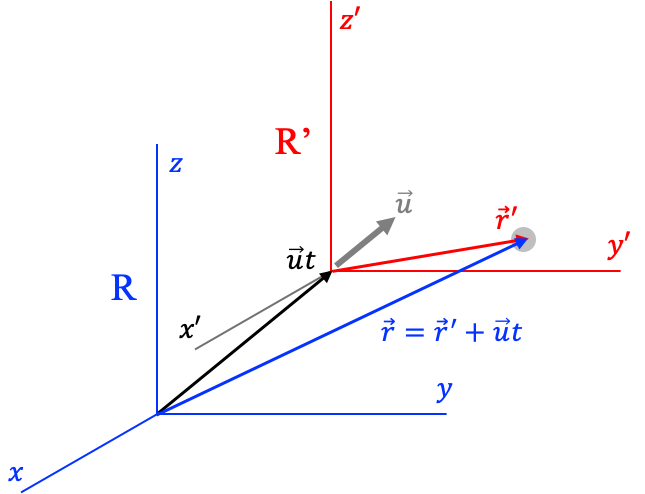
\includegraphics[width=0.5\textwidth]{./figures/square_transformaciones_galileo.png}
\caption{Construcción geométrica para deducir la regla de transformación
de la posición \(\vec r\) de una partícula (circulo gris) entre dos
sistemas de referencia inerciales (que se mueven uno respecto de otro
con velocidad constante
\(\vec u\).\label{fig:transformaciones_galileo}}
\end{figure}

Estas transformaciones fundamentales, permiten escribir las reglas de
transformación para cualquier otras propiedad cinemática, por ejemplo,
para la velocidad y la aceleración:

\begin{eqnarray}
\label{eq:ley_adicion_velocidades}
\vec{v} & = & \vec{v}'+\vec u\\
\label{eq:ley_adicion_aceleraciones}
\vec{a} & = & \vec{a}'
\end{eqnarray}

La Ec. (\ref{eq:ley_adicion_velocidades}) se conoce como la \textbf{ley
de adición de velocidades galileana} y tiene una importancia histórica
en el desarrollo de los postulados de la teoría de la relatividad. La
Ec. (\ref{eq:ley_adicion_aceleraciones}) será importante en la
definición, en las próximas secciones, del concepto de \textbf{sistema
de referencia inercial}.



\hypertarget{ecuacion_movimiento}{%
\subsection{La ecuación de movimiento
(e.d.m.)}\label{ecuacion_movimiento}}

La posición y velocidad de una partícula en cualquier instante futuro
puede predecirse si se resuelve la siguiente ecuación diferencial:

\begin{equation}
\label{eq:edm}
\ddot{\vec r} = \vec a.
\end{equation}

A esta ecuación se la conoce en mecánica como la \textbf{ecuación de
movimiento} y para referirnos a ella, en lo sucesivo, usaremos el
acrónimo e.d.m. o el nombre \texttt{edm} en los algoritmos.

La solución general de esta ecuación es la función de posición de la
partícula \(\vec r(t)\), de la que se pueden deducir posteriormente las
demás cantidades cinemáticas.

La e.d.m. es una ecuación diferencial vectorial de segundo orden con
condiciones iniciales \(\vec{r}(t_0)=r_0\),
\(\dot{\vec r}(t=t_0)=\vec v_0\), es decir, matemáticamente y como
explicamos en la \autoref{ecuaciones_diferenciales}, es un problema
de valor inicial (IVP).

La aceleración \(\vec a\) en la Ec. (\ref{eq:edm}) es una función que
puede depender de varias de las cantidades cinemáticas definidas en la
sección previa. Para la mayoría de las situaciones consideradas en este
texto, sin embargo, asumiremos que la aceleración depende solamente del
tiempo y del estado de la partícula, es decir:

\[
\vec a=\vec a(t,\vec r,\dot{\vec r}).
\]

La e.d.m. puede expresarse también como dos ecuaciones diferenciales
vectoriales de primer orden (\emph{reducción de orden}):

\begin{equation}
\label{eq:edm_primer_orden}
\begin{array}{ccl}
\dot{\vec r} & = &\vec v\\
\dot{\vec v} & = &\vec a(t,\vec r,\vec v)
\end{array}
\end{equation}

Aquí se ha introducido como variable auxiliar la velocidad misma
\(\vec v\equiv\dot{\vec r}\). Escrita de esta manera, la solución al
sistema de ecuaciones diferenciales de la e.d.m. provee simultáneamente
las funciones \(\vec r(t)\) y \(\vec v(t)\). El sistema gana variables,
pero el orden se reduce.

La e.d.m., tanto en la forma (\ref{eq:edm}) como
(\ref{eq:edm_primer_orden}) representa, en realidad, una forma compacta
de escribir un sistema de ecuaciones diferenciales escalares.

En términos de las componentes cartesianas, la e.d.m. de la Ec.
(\ref{eq:edm}) es en realidad un sistema de tres ecuaciones
diferenciales ordinarias de segundo orden:

\begin{equation}
\label{eq:edm_escalar}
\begin{array}{ccl}
\ddot{x} & = &a_x\\
\ddot{y} & = &a_y\\
\ddot{z} & = &a_z\\
\end{array}
\end{equation}

Por su lado la e.d.m. de la Ec. (\ref{eq:edm_primer_orden}) corresponde
a un sistema de 6 ecuaciones diferenciales escalares de primer orden:

\begin{equation}
\label{eq:edm_primer_orden_escalar}
\begin{array}{ccl}
\dot{x} & = &v_x\\
\dot{y} & = &v_y\\
\dot{z} & = &v_z\\
\dot{v_x} & = &a_x(t,x,y,z,v_x,v_y,v_z,y)\\
\dot{v_y} & = &a_y(t,x,y,z,v_x,v_y,v_z,y)\\
\dot{v_z} & = &a_z(t,x,y,z,v_x,v_y,v_z,y)\\
\end{array}
\end{equation}

En está última expresión hemos escrito explícitamente la dependencia de
la aceleración de las componentes del vector de estado, para resaltar el
hecho que el sistema de ecuaciones diferenciales puede ser altamente
\emph{acoplado}.

En términos del vector de estado \(\vec X:(\vec r\;\vec v)^\mathrm{T}\),
la e.d.m. de primer orden (Ec. \ref{eq:edm_primer_orden_escalar}) se
puede escribir como:

\begin{equation}
\label{eq:edm_estado}
\dot{X} = \left( 
\begin{array}{c}
\vec{v} \\ \vec{a}
\end{array}
\right)
\end{equation} donde (abusando de la notación)
\(\vec v:(v_x\;v_y\;v_z)^\mathrm{T}\) y
\(\vec a:(a_x\;a_y\;a_z)^\mathrm{T}\)
\begin{box_note}{Nota}

\textbf{Ecuaciones de movimiento en otros sistemas de coordenadas.}
Ecuaciones análogas a la Ecs.
(\ref{eq:edm_escalar},\ref{eq:edm_primer_orden_escalar}) pueden
escribirse en caso de que la aceleración sea provista en los sistema
coordenadas cilíndricas o esféricas. Para ello deben usarse las
definiciones de velocidad y aceleración, en el sistema de coordenadas
respectivo, que vimos en la \autoref{cantidades_cinematicas}. La
forma explícita de esas ecuaciones diferenciales, sin embargo, no será
tan sencilla como la que escribimos en el caso de las coordenadas
cartesianas. El lector podrá explorar estos casos a través de algunos de
los problemas incluídos al final del capítulo.

\end{box_note}
\hypertarget{integracion_edm}{%
\subsection{Integración de la e.d.m.}\label{integracion_edm}}

La solución o \emph{integración} de la e.d.m. constituye el problema
matemático central de la cinemática y a la larga, el problema más
importante de toda la mecánica incluyendo, naturalmente, la mecánica
celeste.

En los cursos de mecánica newtoniana básica el problema se resuelve
normalmente para dos casos simples:

\begin{enumerate}
\def\labelenumi{\arabic{enumi}.}
\tightlist
\item
  \(\vec a=\vec 0\) que se conoce también como \emph{movimiento
  rectilineo y uniforme.}
\item
  \(\vec a=\vec{a}_0\), donde \(\vec{a}_0\) es un vector constante y que
  se conoce como movimiento rectilíneo uniformemente acelerado.
\end{enumerate}

Si bien estos dos casos son interesantes en la descripción de un amplio
rango de aplicaciones simples (p.e. en el movimiento parabólico), en
situaciones realistas y en particular en las que veremos en la mecánica
celeste, la función \(\vec a\) puede ser mucho más compleja.

En los ejemplos desarrollados a continuación, y que nos serviran para
ilustrar algunos conceptos físicos y matemáticos que usaremos con
regularidad en el resto del libro, consideramos dos situaciones
hipotéticas comúnes, a saber que la \(\vec a\) depende exclusivamente
del tiempo o que esta cantidad depende del vector de estado.

\hypertarget{integracion_cuadraturas}{%
\subsection{Integración por cuadraturas}\label{integracion_cuadraturas}}

\hypertarget{ejemplo-1-movimiento-con-tiruxf3n-constante}{%
\subsubsection{Ejemplo 1: movimiento con tirón
constante}\label{ejemplo-1-movimiento-con-tiruxf3n-constante}}

Considerese el caso simple de una partícula que esta sometida a un tirón
\(\vec{j}:(j_0,0,0)\) constante en el tiempo. Suponga además que en
\(t=0\) la aceleración de la partícula es nula.

En estas condiciones la función de aceleración, en cualquier tiempo, se
puede escribir como:

\[
\vec a(t):(j_0 t,0,0),
\]

Por tanto, la a e.d.m., escrita en términos de las componentes del
vector posición (Ec. \ref{eq:edm_escalar}) será:

\begin{equation}
\label{eq:edm_ejemplo1}
\begin{array}{rcl}
\ddot{x} & = & j_0 t\\
\ddot{y} & = & 0\\
\ddot{z} & = & 0\\
\end{array}
\end{equation}

Si bien una solución a esta ecuación diferencial puede encontrarse
fácilmente por tanteo, p.e. \(x(t)=a t^3+b t^2+c t+d\), un procedimiento
cuidadoso de solución nos permitirá a continuación revelar algunas
propiedades interesantes del sistema dinámico y, más importante aquí,
ilustrar un método de solución de ecuaciones diferenciales que será de
gran utilidad en los siguientes capítulos.

Reescribamos la ecuación para \(x\) en el sistema de Ecs.
(\ref{eq:edm_ejemplo1}) de la forma:

\begin{equation}
\label{eq:edm_ejemplo1_cuadratura}
\frac{\mathrm{d}}{\mathrm{dt}}\dot{x} = \frac{\mathrm{d}}{\mathrm{dt}}\left(\frac{1}{2}ct^2\right).
\end{equation}

La clave de este procedimiento de solución esta en la posibilidad de
escribir, en función de sus respectivas antiderivadas, ambos lados de la
ecuación diferencial. Esta es la razón por la que llamaremos a este
método, \textbf{método de las cuadraturas} en referencia al término que
introdujimos en la \autoref{integrales} para referirnos a la
integral definida de una función.

Reuniendo los términos de la Ec. (\ref{eq:edm_ejemplo1_cuadratura}) en
un mismo lado obtenemos:

\[
\frac{\mathrm{d}}{\mathrm{dt}}\left(\dot{x}-\frac{1}{2}ct^2\right)= 0.
\]

Si bien no hemos resuelto la ecuación todavía, está última manera de
escribirla nos permite que la \emph{fórmula} que aparece entre
paréntesis y que combina la velocidad y el tiempo, sin importar el
estado de la partícula o el instanate de tiempo, siempre será constante
(su derivada con respecto al tiempo es cero):

\begin{equation}
\label{eq:Ix_ejemplo1}
\dot{x}-\frac{1}{2}ct^2 = I_x
\end{equation}

Decimos que \(C_{Ix}(t,\dot x)\equiv\dot{x}-ct^2/2\) es una
\textbf{integral}, una \textbf{cuadratura} o una \textbf{constante de
movimiento} del sistema. En este caso \(I_x\) es el valor que esta
constante adopta para un conjunto específico de condiciones iniciales.
\begin{box_definition}{Definición}{}

\textbf{Constante de movimiento de un sistema dinámico.} Si una función
\(f(t,\vec r,\vec v)\) es tal que:

\[C_I(t,\vec r,\vec v)=I\]

Donde \(I\) es una cantidad que solo depende de las condiciones
iniciales, decimos que \(C_I(t,\vec r,\vec v)\) es una \textbf{constante
de movimiento}. La llamaremos también una \textbf{integral} o
\textbf{cuadratura} del sistema \footnote{En términos rigurosos la
  \emph{constante de movimiento} es la función \(C_I(t,\vec r,\vec v)\)
  no su valor numérico \(I\) que por definición es un número real y por
  lo tanto es constante.}.

\end{box_definition}
Es fácil verificar que otras constantes de movimiento de este sistema
son \(\dot{y}=I_y\) y \(\dot{z}=I_z\).

\hypertarget{ejemplo-2-movimiento-oscilatorio}{%
\subsubsection{Ejemplo 2: movimiento
oscilatorio}\label{ejemplo-2-movimiento-oscilatorio}}

Considere ahora el caso en el que una partícula tiene una aceleración
dada por:

\[
\vec a(t):(-\omega x,0,0),
\] donde \(\omega\) es una cantidad constante. Como vemos, cuando la
partícula se aleja del origen la aceleración apuntá de nuevo hacia allí.
Sabemos que este tipo de aceleración producirá un movimiento
oscilatorio.

En este caso la e.d.m. para la componente \(x\) será:

\[
\ddot{x} = -\omega x.
\]

La integración de esta ecuación por tanteo ya no es tan trivial. Tampoco
lo es intentar exprear ambos lados de la ecuación como derivadas
respecto al tiempo de otras funciones (como lo hicimos para encontrar la
Ec. \ref{eq:edm_ejemplo1_cuadratura}).

Sin embargo, si multiplicamos ambos lados de la ecuación por la función
\(\dot x\):

\[
\dot{x}\ddot{x} = -\omega \dot{x}x,
\] la nueva ecuación puede escribirse, convenientemente, de la forma:

\[
\frac{\mathrm{d}}{\mathrm{dt}}\left(\frac{1}{2}\dot{x}^2\right) = \frac{\mathrm{d}}{\mathrm{dt}}\left(-\frac{1}{2}
\omega x^2\right).
\]

Allí podemos identificar una constante de movimiento del sistema:

\begin{equation}
\label{eq:Ix_ejemplo2}
\frac{1}{2}\dot{x}^2+\frac{1}{2}\omega x^2=I_x.
\end{equation}

Como la multiplicación de la e.d.m. original por la función \(\dot{x}\)
nos permitió encontrar una integral de la ecuación, llamamos a
\(\dot{x}\), un \emph{factor integrante.}

¿De qué sirve encontrar las constantes de movimientode un sistema si lo
que queremos en realidad es hallar la forma explícitas para las
funciones \(\vec r(t)\), \(\vec v(t)\)?

Las constantes de movimiento pueden ofrecernos información sobre la
dinámica del sistema, incluso en situaciones en las que no es posible
obtener una solución. Note, por ejemplo, cuan diferentes son las
constantes de movimiento de los sistemas en los ejemplos 1 y 2. Aunque
no resolvimos ninguno de los dos problemas, sus cuadraturas nos dan
pistas sobre como se relacionan la posición y velocidad de la partícula
en cualquier instante del tiempo. Más adelante mostraremos que es
incluso posible dar una interpretación física a estas constantes (en
términos de cantidades dinámicas conocidas tales como la energía, el
momentum lineal, el momentum angular, o incluso de cantidades
desconocidas pero útiles) y su relevancia para la comprensión del
sistema será aún mayor.

Ahora bien, siendo las cuadraturas \(C(t,\vec r,\vec v)\) funciones de
las variables que deseamos encontrar, si se obtienen suficientes
constantes de movimiento (tantas como variables), habremos,
técnicamente, obtenido la solución.

En otras palabras, un número suficiente de cuadraturas o de constantes
de movimiento permite convertir la solución de una ecuación diferencial,
en la solución a un sistema algebraico de ecuaciones (aquel formado por
las cuadraturas).

Para ilustrarlo volvamos a la e.d.m. del sistema en el ejemplo 1:

\[
\begin{array}{ccl}
\ddot{x} & = & j_0 t\\
\ddot{y} & = & 0\\
\ddot{z} & = & 0\\
\end{array}
\]

Es posible mostrar que este sistema tiene 6 constantes de movimiento (ya
habíamos introducido tres de ellas):

\begin{equation}
\label{eq:constantes_ejemplo1}
\begin{array}{rrl}
\dot{x}-\frac{1}{2}j_0 t^2 & = & I_x \\
\dot{y} & = & I_y \\
\dot{z} & = & I_z\\
x-\frac{1}{6}j_0 t^6-I_x t & = & S_x \\
y-I_y t & = & S_y\\
z-I_z t & = & S_z\\
\end{array}
\end{equation}

El valor de las cantidades \(I_x\), \(I_y\), \(I_z\), \(S_x\), \(S_y\),
\(S_z\) se obtiene reemplazando las condiciones iniciales en el lado
izquierdo de estas ecuaciones.

Si se resuelve simultánemante el sistema de ecuaciones algebraicas
(\ref{eq:constantes_ejemplo1}) se obtiene, finalmente, la solución al
problema original:

\begin{equation}
\label{eq:solucion_ejemplo1}
\begin{array}{rcl}
x(t) & = & \frac{1}{3}j_0 t^3+I_x t+S_x\\
y(t) & = & I_y t+S_y\\
z(t) & = & I_z t+S_z\\
\dot{x}(t) & = & \frac{1}{2}j_0 t^2+I_x\\
\dot{y}(t) & = & I_y \\
\dot{z}(t) & = & I_z\\
\end{array}
\end{equation}

Un procedimiento análogo puede usarse para encontrar la solución a la
e.d.m. del sistema del ejemplo 2 (vea los problemas al final del
capítulo.)

Es posible que nadie escoja un procedimiento tan elaborado para
encontrar la solución a la e.d.m. de estos dos sistemas dinámicos
simples. Claramente, existen procedimiento más sencillos (incluyendo una
solución por tanteo.) Sin embargo, usar el método de las cuadraturas
aquí, con sistemas cuya solución se puede obtener con métodos más
directos, nos permite ilustrar el poder que tiene el método de las
cuadraturas, que será el preferido para encontrar la solución de la
e.d.m. de sistemas dinámicos mucho más complejos en mecánica celeste.



\hypertarget{integracion_numerica_edm}{%
\subsection{Integración numérica de la
e.d.m.}\label{integracion_numerica_edm}}

En aquellos sistemas dinámicos en los que resolver la e.d.m. o encontrar
\emph{todas} las constantes de movimiento (resolver por cuadratura el
sistema), sea imposible matemáticamente o simplemente muy difícil, es
posible buscar una solución aproximada usando los métodos numéricos que
estudiamos al final de la \autoref{ecuaciones_diferenciales}.

Como vimos allí, para hacerlo, es necesario primero escribir la e.d.m.
como el conjunto de 6 ecuaciones diferenciales de primer orden con la
forma general (Ec. \ref{eq:ecuaciones_reducidas}):

\begin{equation}
\label{eq:edm_ecuaciones_reducidas}
\{\dot{Y_i} = f_i(t,\{Y_k\})\}_{6}
\end{equation}

Donde \(Y_i\) (\(i=0,1,2,\ldots,5\)) son las denominadas funciones
auxiliares que reemplazan aquí a las cantidades claves del sistema
dinámico (las componentes de \(\vec r\) y \(\vec v\)). En física,
llamaremos a las Ecs. (\ref{eq:edm_ecuaciones_reducidas}),
\emph{ecuaciones de movimiento reducidas} del sistema o \emph{e.d.m.r.}

Si comparamos la forma general de las e.d.m.r. en la Ec.
(\ref{eq:edm_ecuaciones_reducidas}) con las ecuaciones de primer orden
(\ref{eq:edm_primer_orden_escalar}), podemos hacer la siguiente
identificación para las variables auxiliares \(Y_i\):

\begin{equation}
\label{eq:variables_auxiliares_edm}
\begin{array}{ccc}
Y_0 = x, & Y_1 = y, & Y_2 = z\\
Y_3 = v_x, & Y_4 = v_y, & Y_5 = v_z\\
\end{array}
\end{equation}

Por otro lado, las funciones \(f_i\) serán:

\[
\begin{array}{ccc}
f_0(t,\{Y_k\}) = v_x = Y_3, & f_1(t,\{Y_k\}) = v_y = Y_4, & f_2(t,\{Y_k\}) = v_z = Y_5\\
f_3(t,\{Y_k\}) = a_x, & f_4(t,\{Y_k\}) = a_y, & f_5(t,\{Y_k\}) = a_z\\
\end{array}
\]

Con esta identificación, una forma compacta de escribir las e.d.m.r.,
muy útil a la hora de preparar algoritmos, es:

\begin{equation}
\label{eq:edm_reducidas_particula}
\dot Y_i = 
\left\{
\begin{array}{ccc}
Y_{3+i} & {\rm ,} & 0 \leq i < 3 \\
a_{i-3}  & {\rm ,} & 3\leq i < 6 
\end{array}
\right.
\end{equation} Donde hemos introducido la notación
\(\{a_0,a_1,a_2\}\equiv\{a_x,a_y,a_z\}\).

\hypertarget{integraciuxf3n-numuxe9rica-de-las-e.d.m.-del-ejemplo-1}{%
\subsubsection{Integración numérica de las e.d.m. del ejemplo
1}\label{integraciuxf3n-numuxe9rica-de-las-e.d.m.-del-ejemplo-1}}

El sistema dinámico del ejemplo 1 introducido en
\autoref{integracion_cuadraturas} se caracteriza por tener una
aceleración del tipo \(\vec a:(j_0t,0,0)\). En términos de la
parametrización de la e.d.m.r. en la Ec.
(\ref{eq:edm_reducidas_particula}), esto significa que
\(\{a_0,a_1,a_2\}=(j_0t,0,0)\).

El sistema de ecuaciones diferenciales que describe el sistema puede
implementarse en \texttt{Python} usando la rutina:

    \begin{code}{Algoritmo}{code:edm_ejemplo1}\begin{Verbatim}[fontsize=\small,commandchars=\\\{\}]
\PY{k}{def} \PY{n+nf}{edm\PYZus{}ejemplo1}\PY{p}{(}\PY{n}{Y}\PY{p}{,}\PY{n}{t}\PY{p}{,}\PY{n}{j0}\PY{o}{=}\PY{l+m+mi}{1}\PY{p}{)}\PY{p}{:}
    \PY{n}{dYdt}\PY{o}{=}\PY{p}{[}\PY{l+m+mi}{0}\PY{p}{,}\PY{l+m+mi}{0}\PY{p}{,}\PY{l+m+mi}{0}\PY{p}{,}\PY{l+m+mi}{0}\PY{p}{,}\PY{l+m+mi}{0}\PY{p}{,}\PY{l+m+mi}{0}\PY{p}{]}
    
    \PY{n}{dYdt}\PY{p}{[}\PY{p}{:}\PY{l+m+mi}{3}\PY{p}{]}\PY{o}{=}\PY{n}{Y}\PY{p}{[}\PY{l+m+mi}{3}\PY{p}{:}\PY{p}{]}
    \PY{n}{dYdt}\PY{p}{[}\PY{l+m+mi}{3}\PY{p}{:}\PY{p}{]}\PY{o}{=}\PY{p}{[}\PY{n}{j0}\PY{o}{*}\PY{n}{t}\PY{p}{,}\PY{l+m+mi}{0}\PY{p}{,}\PY{l+m+mi}{0}\PY{p}{]}
    
    \PY{k}{return} \PY{n}{dYdt}
\end{Verbatim}

%%

\end{code}

Aunque al final de la \autoref{ecuaciones_diferenciales} nos
habíamos familiarizado con este tipo de rutinas, el diseño de está en
particular merece algunos comentarios:

\begin{itemize}
\item
  Como sabemos, el propósito de esta rutina es calcular la lista de los
  valores de las funciones \(f_i\) (lado derecho de las Ecs.
  \ref{eq:edm_ecuaciones_reducidas}) que son iguales a las primeras
  derivada en el tiempo de las variables auxiliares \(\dot{Y}_i\). En la
  rutina, para hacer más explícito su significado, hemos decidido llamar
  a esta lista \texttt{dYdt} en lugar de \texttt{f}. Los nombres de las
  variables no afectan la funcionalidad de las rutinas, pero pueden
  hacerla más legible y modificable.
\item
  Para asignar los valores de la lista \texttt{dYdt} hemos aprovechado
  el poder de \texttt{Python} para sacar \emph{trozos}, \emph{porciones}
  o \emph{tajadas} (\emph{slices} en inglés) de listas y arreglos. Así
  el trozo \texttt{dYdt{[}:3{]}} corresponde a las primeras tres
  componentes \texttt{dYdt{[}0{]}}, \texttt{dYdt{[}1{]}},
  \texttt{dYdt{[}2{]}} (nótese que, por empezar en 0, este trozo no
  incluye la componente \texttt{dYdt{[}3{]}}.) Por otra parte el trozo
  \texttt{Y{[}3:{]}} de esta lista, corresponde a las componentes
  \texttt{Y{[}3{]}}, \texttt{Y{[}4{]}}, \texttt{Y{[}5{]}}. Por tanto, la
  igualdad \texttt{dYdt{[}:3{]}=dYdt{[}3:{]}} equivale a escribir
  explícitamente \texttt{dYdt{[}0{]}=Y{[}3{]}},
  \texttt{dYdt{[}1{]}=Y{[}4{]}}, \texttt{dYdt{[}2{]}=Y{[}5{]}} que
  justamente implementa la parte \(\dot{Y}_i=Y_{i+3}\) de la Ec.
  (\ref{eq:edm_reducidas_particula})
\end{itemize}

Una vez escrita la rutina, la solución se obtiene siguiendo los
algoritmos introducidos al final de la
\autoref{ecuaciones_diferenciales}:

    \begin{code}{}{}\begin{Verbatim}[fontsize=\small,commandchars=\\\{\}]
\PY{c+c1}{\PYZsh{}Valor del tiron}
\PY{n}{j0}\PY{o}{=}\PY{l+m+mf}{0.5}

\PY{c+c1}{\PYZsh{}Condiciones iniciales}
\PY{k+kn}{from} \PY{n+nn}{numpy} \PY{k}{import} \PY{n}{array}
\PY{n}{Yos}\PY{o}{=}\PY{n}{array}\PY{p}{(}\PY{p}{[}\PY{l+m+mi}{1}\PY{p}{,}\PY{l+m+mi}{0}\PY{p}{,}\PY{l+m+mi}{0}\PY{p}{,}\PY{o}{\PYZhy{}}\PY{l+m+mi}{3}\PY{p}{,}\PY{l+m+mi}{0}\PY{p}{,}\PY{l+m+mi}{0}\PY{p}{]}\PY{p}{)}

\PY{c+c1}{\PYZsh{}Tiempos para obtener la solución}
\PY{k+kn}{from} \PY{n+nn}{numpy} \PY{k}{import} \PY{n}{linspace}
\PY{n}{ts}\PY{o}{=}\PY{n}{linspace}\PY{p}{(}\PY{l+m+mf}{0.0}\PY{p}{,}\PY{l+m+mf}{5.0}\PY{p}{,}\PY{l+m+mi}{20}\PY{p}{)}

\PY{c+c1}{\PYZsh{}Solución con odeint}
\PY{k+kn}{from} \PY{n+nn}{scipy}\PY{n+nn}{.}\PY{n+nn}{integrate} \PY{k}{import} \PY{n}{odeint}
\PY{n}{Ys}\PY{o}{=}\PY{n}{odeint}\PY{p}{(}\PY{n}{edm\PYZus{}ejemplo1}\PY{p}{,}\PY{n}{Yos}\PY{p}{,}\PY{n}{ts}\PY{p}{,}\PY{n}{args}\PY{o}{=}\PY{p}{(}\PY{n}{j0}\PY{p}{,}\PY{p}{)}\PY{p}{)}
\end{Verbatim}

%%

\end{code}
\vspace{-1em}

%%hidecode


    \begin{Verbatim}[fontsize=\small,commandchars=\\\{\}]
Solucion, Ys:
[[ 1.          0.          0.         -3.          0.          0.        ]
 [ 0.21204503  0.          0.         -2.98268698  0.          0.        ]
 [-0.56679785  0.          0.         -2.93074792  0.          0.        ]
 [-1.32741651  0.          0.         -2.84418283  0.          0.        ]
 [-2.06069881  0.          0.         -2.72299169  0.          0.        ]]
{\ldots}
\end{Verbatim}

Podemos, finalmente, visualizar la solución a la e.d.m.r. haciendo un
gráfico de la coordenada \(x\) (columna \texttt{Ys{[}:,0{]}} de la
matriz de solución) como función del tiempo \texttt{ts}:
%%HIDE%%
    \begin{code}{Algoritmo}{code:ejemplo1_grafico_solucion}\begin{Verbatim}[fontsize=\small,commandchars=\\\{\}]
\PY{k+kn}{import} \PY{n+nn}{matplotlib}\PY{n+nn}{.}\PY{n+nn}{pyplot} \PY{k}{as} \PY{n+nn}{plt}
\PY{n}{plt}\PY{o}{.}\PY{n}{figure}\PY{p}{(}\PY{p}{)}\PY{p}{;}
\PY{n}{plt}\PY{o}{.}\PY{n}{plot}\PY{p}{(}\PY{n}{ts}\PY{p}{,}\PY{n}{Ys}\PY{p}{[}\PY{p}{:}\PY{p}{,}\PY{l+m+mi}{0}\PY{p}{]}\PY{p}{,}\PY{l+s+s1}{\PYZsq{}}\PY{l+s+s1}{ko}\PY{l+s+s1}{\PYZsq{}}\PY{p}{)}\PY{p}{;}

\PY{n}{plt}\PY{o}{.}\PY{n}{xlabel}\PY{p}{(}\PY{l+s+s2}{\PYZdq{}}\PY{l+s+s2}{\PYZdl{}t\PYZdl{}}\PY{l+s+s2}{\PYZdq{}}\PY{p}{)}\PY{p}{;}
\PY{n}{plt}\PY{o}{.}\PY{n}{ylabel}\PY{p}{(}\PY{l+s+s2}{\PYZdq{}}\PY{l+s+s2}{\PYZdl{}x\PYZdl{}}\PY{l+s+s2}{\PYZdq{}}\PY{p}{)}\PY{p}{;}
\PY{n}{plt}\PY{o}{.}\PY{n}{show}\PY{p}{(}\PY{p}{)}\PY{p}{;}
\end{Verbatim}

%%figcaption::show::La figura muestra la solución numérica a la e.d.m. de un sistema sometido a un tirón constante $\vec j=j_0\hat{e}_x$.

\tcblower
\footnotesize
\em ver Figura \ref{fig:code:ejemplo1_grafico_solucion}
\end{code}

    \begin{center}

\begin{figure}[ht!]
\centering
    \adjustimage{max size={0.8\linewidth}{0.8\paperheight}}{combined_files/combined_579_0.png}
\caption{Figura correspondiente al código \ref{code:ejemplo1_grafico_solucion}. La figura muestra la solución numérica a la e.d.m. de un sistema sometido a un tirón constante $\vec j=j_0\hat{e}_x$.\label{fig:code:ejemplo1_grafico_solucion}}
\end{figure}

    \end{center}
%{ \hspace*{\fill} \\}
    
¿Cómo saber si la solución obtenida con \texttt{odeint} y mostrada en la
\autoref{fig:code:ejemplo1_grafico_solucion} es la correcta?

Existen dos manera de comprobarlo. La primera es verificar que las
posiciones y velocidades obtenidas satisfagan las constantes de
movimiento que escribimos en las Ecs. (\ref{eq:constantes_ejemplo1}).

Así por ejemplo, podemos verificar que el valor de \(I_x\) y \(S_x\)
sean efectivamente constantes:

    \begin{code}{}{}\begin{Verbatim}[fontsize=\small,commandchars=\\\{\}]
\PY{c+c1}{\PYZsh{}Extraemos los valores de x y dxdt de la solución}
\PY{n}{xs}\PY{o}{=}\PY{n}{Ys}\PY{p}{[}\PY{p}{:}\PY{p}{,}\PY{l+m+mi}{0}\PY{p}{]}
\PY{n}{xdots}\PY{o}{=}\PY{n}{Ys}\PY{p}{[}\PY{p}{:}\PY{p}{,}\PY{l+m+mi}{3}\PY{p}{]}

\PY{c+c1}{\PYZsh{}Fórmula de la constante C\PYZus{}Ix}
\PY{n}{C\PYZus{}Ixs}\PY{o}{=}\PY{n}{xdots}\PY{o}{\PYZhy{}}\PY{l+m+mf}{0.5}\PY{o}{*}\PY{n}{j0}\PY{o}{*}\PY{n}{ts}\PY{o}{*}\PY{o}{*}\PY{l+m+mi}{2}

\PY{c+c1}{\PYZsh{}Fórmula de la constante C\PYZus{}Sx}
\PY{n}{C\PYZus{}Sxs}\PY{o}{=}\PY{n}{xs}\PY{o}{\PYZhy{}}\PY{p}{(}\PY{l+m+mf}{1.}\PY{o}{/}\PY{l+m+mi}{6}\PY{p}{)}\PY{o}{*}\PY{n}{j0}\PY{o}{*}\PY{n}{ts}\PY{o}{*}\PY{o}{*}\PY{l+m+mi}{3}\PY{o}{\PYZhy{}}\PY{n}{C\PYZus{}Ixs}\PY{o}{*}\PY{n}{ts}
\end{Verbatim}

%%

\end{code}
\vspace{-1em}

%%hidecode


    \begin{Verbatim}[fontsize=\small,commandchars=\\\{\}]
Valores de C\_Ix = [-3. -3. -3. -3. -3.]{\ldots}
Valores de C\_Sx = [1. 1. 1. 1. 1.]{\ldots}
\end{Verbatim}

Comprobamos así que las fórmulas \(C_{Ix}=\dot{x}-j_0t^2/2\) y
\(C_{Sx}=x-j_0t^3/6-I_x t\), tienen el mismo valor para todos los
tiempos en los que integramos la e.d.m.r., es decir, son, por
definición, constantes de movimiento. La solución numérica, por
tanto,satisface nuestras expectativas matemáticas.

La segunda manera de verificar que nuestra solución numérica coincida
con la analítica es compararla con la solución explícita escrita en las
Ecs. (\ref{eq:solucion_ejemplo1}):

\[
x(t)=\frac{1}{6}j_0 t^3+I_x t+S_x
\]

Aquí, los valores de \(I_x\) y \(S_x\) pueden obtenerse de las
condiciones iniciales.

Una comparación gráfica entre ambas soluciones se consigue con este
algoritmo:

    \begin{code}{Algoritmo}{code:compara_numerica_analitica}\begin{Verbatim}[fontsize=\small,commandchars=\\\{\}]
\PY{c+c1}{\PYZsh{}Valor de las constantes de movimiento }
\PY{n}{Ix}\PY{o}{=}\PY{n}{Yos}\PY{p}{[}\PY{l+m+mi}{3}\PY{p}{]}\PY{o}{\PYZhy{}}\PY{l+m+mf}{0.5}\PY{o}{*}\PY{n}{j0}\PY{o}{*}\PY{n}{ts}\PY{p}{[}\PY{l+m+mi}{0}\PY{p}{]}\PY{o}{*}\PY{o}{*}\PY{l+m+mi}{2}
\PY{n}{Sx}\PY{o}{=}\PY{n}{Yos}\PY{p}{[}\PY{l+m+mi}{0}\PY{p}{]}\PY{o}{\PYZhy{}}\PY{p}{(}\PY{l+m+mf}{1.}\PY{o}{/}\PY{l+m+mi}{6}\PY{p}{)}\PY{o}{*}\PY{n}{j0}\PY{o}{*}\PY{n}{ts}\PY{p}{[}\PY{l+m+mi}{0}\PY{p}{]}\PY{o}{*}\PY{o}{*}\PY{l+m+mi}{3}\PY{o}{+}\PY{n}{Ix}\PY{o}{*}\PY{n}{ts}\PY{p}{[}\PY{l+m+mi}{0}\PY{p}{]}

\PY{c+c1}{\PYZsh{}Lista más completa de valores del tiempo}
\PY{k+kn}{from} \PY{n+nn}{numpy} \PY{k}{import} \PY{n}{linspace}
\PY{n}{tas}\PY{o}{=}\PY{n}{linspace}\PY{p}{(}\PY{n}{ts}\PY{p}{[}\PY{l+m+mi}{0}\PY{p}{]}\PY{p}{,}\PY{n}{ts}\PY{p}{[}\PY{o}{\PYZhy{}}\PY{l+m+mi}{1}\PY{p}{]}\PY{p}{,}\PY{l+m+mi}{100}\PY{p}{)}

\PY{c+c1}{\PYZsh{}Solución analítica}
\PY{n}{xs}\PY{o}{=}\PY{p}{(}\PY{l+m+mf}{1.}\PY{o}{/}\PY{l+m+mi}{6}\PY{p}{)}\PY{o}{*}\PY{n}{j0}\PY{o}{*}\PY{n}{tas}\PY{o}{*}\PY{o}{*}\PY{l+m+mi}{3}\PY{o}{+}\PY{n}{Ix}\PY{o}{*}\PY{n}{tas}\PY{o}{+}\PY{n}{Sx}

\PY{c+c1}{\PYZsh{}Gráfico}
\PY{n}{plt}\PY{o}{.}\PY{n}{figure}\PY{p}{(}\PY{p}{)}\PY{p}{;}
\PY{n}{plt}\PY{o}{.}\PY{n}{plot}\PY{p}{(}\PY{n}{ts}\PY{p}{,}\PY{n}{Ys}\PY{p}{[}\PY{p}{:}\PY{p}{,}\PY{l+m+mi}{0}\PY{p}{]}\PY{p}{,}\PY{l+s+s1}{\PYZsq{}}\PY{l+s+s1}{ko}\PY{l+s+s1}{\PYZsq{}}\PY{p}{,}\PY{n}{label}\PY{o}{=}\PY{l+s+s2}{\PYZdq{}}\PY{l+s+s2}{Solución numérica}\PY{l+s+s2}{\PYZdq{}}\PY{p}{)}\PY{p}{;}
\PY{n}{plt}\PY{o}{.}\PY{n}{plot}\PY{p}{(}\PY{n}{tas}\PY{p}{,}\PY{n}{xs}\PY{p}{,}\PY{l+s+s1}{\PYZsq{}}\PY{l+s+s1}{r\PYZhy{}}\PY{l+s+s1}{\PYZsq{}}\PY{p}{,}\PY{n}{label}\PY{o}{=}\PY{l+s+s2}{\PYZdq{}}\PY{l+s+s2}{Solución analítica}\PY{l+s+s2}{\PYZdq{}}\PY{p}{)}\PY{p}{;}

\PY{n}{plt}\PY{o}{.}\PY{n}{xlabel}\PY{p}{(}\PY{l+s+s2}{\PYZdq{}}\PY{l+s+s2}{\PYZdl{}t\PYZdl{}}\PY{l+s+s2}{\PYZdq{}}\PY{p}{)}
\PY{n}{plt}\PY{o}{.}\PY{n}{ylabel}\PY{p}{(}\PY{l+s+s2}{\PYZdq{}}\PY{l+s+s2}{\PYZdl{}x\PYZdl{}}\PY{l+s+s2}{\PYZdq{}}\PY{p}{)}
\PY{n}{plt}\PY{o}{.}\PY{n}{legend}\PY{p}{(}\PY{p}{)}\PY{p}{;}
\PY{n}{plt}\PY{o}{.}\PY{n}{show}\PY{p}{(}\PY{p}{)}\PY{p}{;}
\end{Verbatim}

%%figcaption::show::Comparación de la solución numérica (puntos) y la solución analítica (línea continua) de la e.d.m. de un sistema con tirón constante $j_0=0.5$

\tcblower
\footnotesize
\em ver Figura \ref{fig:code:compara_numerica_analitica}
\end{code}

    \begin{center}

\begin{figure}[ht!]
\centering
    \adjustimage{max size={0.8\linewidth}{0.8\paperheight}}{combined_files/combined_585_0.png}
\caption{Figura correspondiente al código \ref{code:compara_numerica_analitica}. Comparación de la solución numérica (puntos) y la solución analítica (línea continua) de la e.d.m. de un sistema con tirón constante $j_0=0.5$.\label{fig:code:compara_numerica_analitica}}
\end{figure}

    \end{center}
%{ \hspace*{\fill} \\}
    
La coincidencia entre la solución analítica y la solución numérica
mostrada en la \autoref{fig:code:compara_numerica_analitica} es casi
perfecta.

\hypertarget{integraciuxf3n-numuxe9rica-de-las-e.d.m.-del-ejemplo-2}{%
\subsubsection{Integración numérica de las e.d.m. del ejemplo
2}\label{integraciuxf3n-numuxe9rica-de-las-e.d.m.-del-ejemplo-2}}

Usando las mismas herramientas y algoritmos análogos a los usados antes,
podemos ahora resolver el ejemplo 2 de la \autoref{integracion_edm}.

De nuevo, las ecuaciones reducidas del sistema serán, como en el ejemplo
1, las mismas de la Ec. (\ref{eq:edm_reducidas_particula}), pero ahora
\(\{a_i\}=\{-\omega Y_0,0,0\}\) (nótese que hemos reemplazado \(x\) por
la variable auxiliar \(Y_0\) de acuerdo a las reglas en Ec.
\ref{eq:variables_auxiliares_edm}).

La rutina que implementa las \texttt{edm} en este caso será:

    \begin{code}{}{}\begin{Verbatim}[fontsize=\small,commandchars=\\\{\}]
\PY{k}{def} \PY{n+nf}{edm\PYZus{}ejemplo2}\PY{p}{(}\PY{n}{Y}\PY{p}{,}\PY{n}{t}\PY{p}{,}\PY{n}{omega}\PY{p}{)}\PY{p}{:}
    \PY{n}{dYdt}\PY{o}{=}\PY{p}{[}\PY{l+m+mi}{0}\PY{p}{,}\PY{l+m+mi}{0}\PY{p}{,}\PY{l+m+mi}{0}\PY{p}{,}\PY{l+m+mi}{0}\PY{p}{,}\PY{l+m+mi}{0}\PY{p}{,}\PY{l+m+mi}{0}\PY{p}{]}
    
    \PY{n}{dYdt}\PY{p}{[}\PY{p}{:}\PY{l+m+mi}{3}\PY{p}{]}\PY{o}{=}\PY{n}{Y}\PY{p}{[}\PY{l+m+mi}{3}\PY{p}{:}\PY{p}{]}
    \PY{n}{dYdt}\PY{p}{[}\PY{l+m+mi}{3}\PY{p}{:}\PY{p}{]}\PY{o}{=}\PY{p}{[}\PY{o}{\PYZhy{}}\PY{n}{omega}\PY{o}{*}\PY{n}{Y}\PY{p}{[}\PY{l+m+mi}{0}\PY{p}{]}\PY{p}{,}\PY{l+m+mi}{0}\PY{p}{,}\PY{l+m+mi}{0}\PY{p}{]}
    
    \PY{k}{return} \PY{n}{dYdt}
\end{Verbatim}

%%

\end{code}

La solución al sistema, una comprobación de que la constante \(C_{Ix}\)
en la Ec. (\ref{eq:Ix_ejemplo2}) es en realidad una constante, y una
gráfica de la posición como función del tiempo, se muestra en el
siguiente algoritmo:

    \begin{code}{Algoritmo}{code:solucion_numerica_ejemplo2}\begin{Verbatim}[fontsize=\small,commandchars=\\\{\}]
\PY{c+c1}{\PYZsh{}Propiedades del sistema}
\PY{n}{omega}\PY{o}{=}\PY{l+m+mf}{2.5}

\PY{c+c1}{\PYZsh{}Condiciones iniciales}
\PY{k+kn}{from} \PY{n+nn}{numpy} \PY{k}{import} \PY{n}{array}
\PY{n}{Yos}\PY{o}{=}\PY{n}{array}\PY{p}{(}\PY{p}{[}\PY{l+m+mi}{1}\PY{p}{,}\PY{l+m+mi}{0}\PY{p}{,}\PY{l+m+mi}{0}\PY{p}{,}\PY{l+m+mi}{0}\PY{p}{,}\PY{l+m+mi}{0}\PY{p}{,}\PY{l+m+mi}{0}\PY{p}{]}\PY{p}{)}

\PY{c+c1}{\PYZsh{}Tiempos}
\PY{k+kn}{from} \PY{n+nn}{numpy} \PY{k}{import} \PY{n}{linspace}
\PY{n}{ts}\PY{o}{=}\PY{n}{linspace}\PY{p}{(}\PY{l+m+mi}{0}\PY{p}{,}\PY{l+m+mf}{10.0}\PY{p}{,}\PY{l+m+mi}{100}\PY{p}{)}
\PY{c+c1}{\PYZsh{}Solución}
\PY{n}{Ys}\PY{o}{=}\PY{n}{odeint}\PY{p}{(}\PY{n}{edm\PYZus{}ejemplo2}\PY{p}{,}\PY{n}{Yos}\PY{p}{,}\PY{n}{ts}\PY{p}{,}\PY{n}{args}\PY{o}{=}\PY{p}{(}\PY{n}{omega}\PY{p}{,}\PY{p}{)}\PY{p}{)}

\PY{c+c1}{\PYZsh{}Constante de movimiento}
\PY{n}{xs}\PY{o}{=}\PY{n}{Ys}\PY{p}{[}\PY{p}{:}\PY{p}{,}\PY{l+m+mi}{0}\PY{p}{]}
\PY{n}{xdots}\PY{o}{=}\PY{n}{Ys}\PY{p}{[}\PY{p}{:}\PY{p}{,}\PY{l+m+mi}{3}\PY{p}{]}
\PY{n}{C\PYZus{}Ixs}\PY{o}{=}\PY{l+m+mf}{0.5}\PY{o}{*}\PY{n}{xdots}\PY{o}{*}\PY{o}{*}\PY{l+m+mi}{2}\PY{o}{+}\PY{l+m+mf}{0.5}\PY{o}{*}\PY{n}{omega}\PY{o}{*}\PY{n}{xs}\PY{o}{*}\PY{o}{*}\PY{l+m+mi}{2}

\PY{c+c1}{\PYZsh{}Gráfico}
\PY{n}{fig}\PY{o}{=}\PY{n}{plt}\PY{o}{.}\PY{n}{figure}\PY{p}{(}\PY{p}{)}\PY{p}{;}
\PY{n}{plt}\PY{o}{.}\PY{n}{plot}\PY{p}{(}\PY{n}{ts}\PY{p}{,}\PY{n}{Ys}\PY{p}{[}\PY{p}{:}\PY{p}{,}\PY{l+m+mi}{0}\PY{p}{]}\PY{p}{)}\PY{p}{;}

\PY{n}{plt}\PY{o}{.}\PY{n}{xlabel}\PY{p}{(}\PY{l+s+s2}{\PYZdq{}}\PY{l+s+s2}{\PYZdl{}t\PYZdl{}}\PY{l+s+s2}{\PYZdq{}}\PY{p}{)}\PY{p}{;}
\PY{n}{plt}\PY{o}{.}\PY{n}{ylabel}\PY{p}{(}\PY{l+s+s2}{\PYZdq{}}\PY{l+s+s2}{\PYZdl{}x\PYZdl{}}\PY{l+s+s2}{\PYZdq{}}\PY{p}{)}\PY{p}{;}
\PY{n}{plt}\PY{o}{.}\PY{n}{show}\PY{p}{(}\PY{p}{)}\PY{p}{;}
\end{Verbatim}

%%figcaption::show::Solución numérica de la e.d.m. de un sistema dinámico con aceleracion $\vec a:(-2.5x,0,0)$.

\tcblower
\footnotesize
\em ver Figura \ref{fig:code:solucion_numerica_ejemplo2}
\end{code}

    \begin{center}

\begin{figure}[ht!]
\centering
    \adjustimage{max size={0.8\linewidth}{0.8\paperheight}}{combined_files/combined_591_0.png}
\caption{Figura correspondiente al código \ref{code:solucion_numerica_ejemplo2}. Solución numérica de la e.d.m. de un sistema dinámico con aceleracion $\vec a:(-2.5x,0,0)$.\label{fig:code:solucion_numerica_ejemplo2}}
\end{figure}

    \end{center}
%{ \hspace*{\fill} \\}
    \vspace{-1em}

%%hidecode

\vspace{-1em}

%%hidecode


    \begin{Verbatim}[fontsize=\small,commandchars=\\\{\}]
Valores de C\_Ix: [1.25 1.25 1.25 1.25 1.25]{\ldots}
\end{Verbatim}

Podemos comprobar al examinar la
\autoref{fig:code:solucion_numerica_ejemplo2} nuestra intuición inicial
de que la dinámica del sistema correspondía a la de un movimiento
oscilatorio.



\hypertarget{dinamica}{%
\section{Dinámica}\label{dinamica}}

\hypertarget{cantidades_dinamicas}{%
\subsection{Cantidades dinámicas}\label{cantidades_dinamicas}}

Las cantidades dinámicas son aquellas que son requeridas para describir
la relación entre las causas del movimiento y su descripción. Las más
usadas se desciben a continuación:

\begin{itemize}
\item
  \textbf{Masa, \(m\)}.

  \begin{itemize}
  \tightlist
  \item
    Definición: Escalar que mide (en el contexto de la mecánica
    Newtoniana): (1) la cantidad de materia contenida en un cuerpo,
    \(m=\int \rho dV\) donde \(\rho\) es la densidad y la integral se
    realiza sobre el volumen del cuerpo, (2) la \emph{inercia} o
    resistencia del cuerpo a moverse y (3) la intensidad de la atracción
    gravitacional que experimenta o produce en otros cuerpos (ver la
    \autoref{masa_equivalencia}).
  \item
    Patrón: \([m]=\)M.
  \item
    Unidad del SI\footnote{Sistema Internacional de Unidades}: kg.
  \end{itemize}
\end{itemize}

\begin{itemize}
\tightlist
\item
  \textbf{Momento lineal, \(p\)}:

  \begin{itemize}
  \tightlist
  \item
    Definción: \(\vec p\equiv m\vec v=m\dot{\vec{r}}\).
  \item
    Patrón: \([p]=\)M L T\(^{-1}\).
  \item
    Unidad del SI: kg m s\(^{-1}\).
  \end{itemize}
\end{itemize}

\begin{itemize}
\tightlist
\item
  \textbf{Momentum angular, \(L\)}:

  \begin{itemize}
  \tightlist
  \item
    Definción: \(\vec L\equiv \vec r\times\vec p\).
  \item
    Una propiedad para partículas puntuales (\(m\) constante):
    \(\vec L = m \vec r\times\dot{\vec r}\).
  \item
    Patrón: \([L]=\)M L\(^2\) T\(^{-1}\).
  \item
    Unidad del SI: kg m\(^2\) s\(^{-1}\).
  \end{itemize}
\end{itemize}

\begin{itemize}
\tightlist
\item
  \textbf{Fuerza resultante, \(\cal F\)}:

  \begin{itemize}
  \tightlist
  \item
    Definción: \(\vec{\cal F}\equiv \dot{\vec{p}}\).
  \item
    Una propiedad para partículas puntuales (\(m\) constante),
    \(\vec{\cal F}=m \ddot{\vec r}\).
  \item
    Patrón: \([\cal F]=\)M L T\(^{-2}\).
  \item
    Unidad del SI: kg m s\(^{-2}\) \(\equiv\) N (Newton).
  \end{itemize}
\end{itemize}

\begin{itemize}
\tightlist
\item
  \textbf{Momento de fuerza o torca, \(\vec{\tau}\)}:

  \begin{itemize}
  \tightlist
  \item
    Definción: \(\vec \tau\equiv \vec r\times \vec{\cal F}\).
  \item
    Una propiedad para partículas puntuales (\(m\) constante):
    \(\vec \tau = \dot{\vec{L}}\).
  \item
    Patrón: \([\tau]=\)M L\(^{2}\) T\(^{-2}\).
  \item
    Unidad del SI: kg m\(^2\) s\(^{-2}\).
  \end{itemize}
\end{itemize}

\begin{itemize}
\tightlist
\item
  \textbf{Energía cinética o \emph{vis viva}, \(K\)}:

  \begin{itemize}
  \tightlist
  \item
    Definción: \(K\equiv m \vec{v}^2/2\).
  \item
    Patrón: \([K]=\)M L\(^{2}\) T\(^{-2}\).
  \item
    Unidad del SI: kg m\(^2\) s\(^{-2}\) \(\equiv\) J (\emph{Joule},
    pronunciado \hreffoot{https://forvo.com/search/Joule/fr/}{``syul''}).
  \end{itemize}
\end{itemize}

\begin{itemize}
\tightlist
\item
  \textbf{Trabajo, \(W\)}:

  \begin{itemize}
  \tightlist
  \item
    Definición: \(W = \int {\cal F}(\vec r)\cdot\mathrm{d}\vec{r}\).
  \item
    Patrón: \([W]=\)M L\(^{2}\) T\(^{-2}\).
  \item
    Unidad del SI: J.
  \end{itemize}
\end{itemize}

\hypertarget{particulas_fuerzas}{%
\subsection{Partículas y fuerzas}\label{particulas_fuerzas}}

Hay tres conceptos centrales en la dinámica newtoniana: partícula,
fuerza y masa.

Entenderemos aquí por partícula o \textbf{partícula puntual} a una
entidad material de tamaño insignificante, sin estructura, ni volumen
(independientemente de que se las represente gráficamente como esferas.)

Un sistema de muchas partículas puntuales puede formar: una ``nube'', un
cuerpo (rígido o elástico) o un fluído. En lo que resta de este libro
nos concentraremos únicamente en la dinámica de partículas individuales
o ``nubes'' de partículas.
\begin{box_note}{Nota}

\textbf{Masa constante para partículas puntuales.} A diferencia de lo
que pasa con un sistema de partículas, en la que el número de
constituyentes puede variar debido al intercambio de materia con otros
sistemas, en lo sucesivo asumiremos que la masa de las partículas
puntuales es constante en el tiempo e independiente del sistema de
referencia.

\end{box_note}
El concepto de fuerza es uno de los más esquivos de la Física
\cite{Wilczek2004Force}. Para los propósitos de este libro nos
apegaremos a ``definiciones'' practicas del concepto, cercanas pero no
en exceso a las introducidas originalmente por Newton en los
\emph{Principia}.

Distingumos dos cantidades físicas a las que llamaremos \emph{fuerza}:

\begin{itemize}
\item
  La \textbf{fuerza resultante}, \(\vec{\cal F}\) es el nombre que
  daremos aquí a la razón instantánea de cambio en el momento lineal,
  \({\cal F}\equiv\dot{\vec p}\), independiente de cuál sea la causa de
  ese cambio.
\item
  La \textbf{fuerza aplicada}, \(\vec F\), es un concepto eminentemente
  newtoniano y, en términos modernos, pobremente definido. En general,
  la fuerza aplicada es una medida la intensidad de la
  \emph{interacción} entre una partícula y su entorno (otras partículas,
  medios materiales o campos). El valor de la fuerza aplicada
  difícilmente puede derivarse de primeros principios y normalmente se
  postula (p.e. la fuerza gravitacional) o se construye a partir de
  modelos simplificados de las interacciones (p.e. las fuerzas de
  fricción.)
\end{itemize}

En la mecánica Newtoniana se reconocen dos tipos básicos de \emph{fuerza
aplicada}:

\begin{itemize}
\item
  \textbf{Fuerzas de contacto}: Fuerzas que resultan de la interacción
  por contacto de una partícula con otras partículas (p.e. fuerzas en
  choques), con medios (p.e. fricción en un fluído) o con fronteras
  materiales (p.e. fuerzas normales o de fricción).
\item
  \textbf{Fuerzas de campo o de acción a distancia}: Fuerzas que
  resultan de la interacción de las partículas con otras partículas o
  cuerpos materiales, sin que medie el contacto directo (a distancia);
  también están en este grupo las fuerzas que resultan de la interacción
  con un \emph{campo} (por ejemplo los campos electromagnéticos).
\end{itemize}

Existe una tercera categoría de fuerzas, pero a diferencia de las
anteriores no corresponden a \emph{fuerzas aplicadas} sino un tipo
específico de \emph{fuerzas resultantes}:

\begin{itemize}
\tightlist
\item
  \textbf{Fuerzas ficticias}: Son fuerzas resultantes que se manifiestan
  al estudiar la dinámica en ciertos sistema de referencia (por ejemplo
  en sistemas de referencia rotantes). Entre ellas están la \emph{fuerza
  centrífuga} y la \emph{fuerza de Coriolis} que estudiaremos en la
  \autoref{dinamica_rotantes}. El adjetivo de \emph{ficticias} viene
  precisamente del hecho de que no son producto de interacciónes con
  otras partículas o cuerpos materiales.
\end{itemize}

\hypertarget{sistemas_referencia_inerciales}{%
\subsection{Sistemas de referencia
inerciales}\label{sistemas_referencia_inerciales}}

La introducción del concepto de fuerza ficticia permite definir un
concepto central en la mecánica newtoniana:
\begin{box_definition}{Definición}{box:def:sistemas.inerciales}

\textbf{Sistema de referencia inercial.} Decimos que un sistema de
referencia es inercial si todas las fuerzas resultantes en el sistema
son causadas por fuerzas aplicadas, es decir si todos los cambios en los
momentos lineales de las partículas pueden rastrearse hasta
interacciones entre ellas, con medios materiales o con campos.

\end{box_definition}
Demostrar en la práctica que un sistema de referencia es inercial, que
implica rastrear todas las causas físicas de los cambios en los momentos
lineales de las partículas de un sistema de prueba, puede ser muy
complicado sino imposible. Existe, sin embargo, un teorema que puede ser
de gran utilidad para este propósito:
\begin{box_theorem}{Proposición}{box:teo:sistemas.inerciales}

\textbf{Sistemas de referencia con velocidad relativa constante.} Si un
sistema de referencia \(R\) se mueve con velocidad constante respecto a
un sistema de referencia inercial \(I\), entonces R es también un
sistema de referencia inercial.

\end{box_theorem}
Este teorema es una consecuencia directa de las transformaciones de
Galileo que postulamos en la \autoref{sistemas_referencia} (ver
sección de problemas al final del capítulo).

Para los propósitos de la mecánica Newtoniana, basta que identifiquemos
al menos un sistema de referencia inercial en el Universo para que,
midiendo la velocidad relativa respecto a él, podamos determinar si
otros sistemas de referencia son también inerciales.

En la práctica la ``inercialidad'' de un sistema de referencia (el
centro de masa del sistema solar, el centro de la galaxia, la radiación
cósmica de fondo) se postula (o se considera como una aproximación en
los modelos) y a partir de ellos a través del Teorema
(\ref{box:teo:sistemas_inerciales}) se construyen otros sistemas de
referencia inerciales.


\begin{box_history}{Un pooco de historia}{}{nofloat}
\small

\textbf{Los \emph{Principia} de Newton.} En abril de 1687 y después de
trabajar tan solo durante 18 meses, Newton completo las 550 páginas del
manuscrito que se convertiría en la primera edición de sus
\emph{Philosophiæ Naturalis Principia Mathematica} (Principios
Matemáticos de la Filosofía Natural, ver
\autoref{fig:principia})\footnote{La copia digital de una primera
  edición del libro puede leerse en línea en la biblioteca digital de la
  Universidad de Cambridge
  http://cudl.lib.cam.ac.uk/view/PR-ADV-B-00039-00001/1}. A pesar del
breve lapso de tiempo en el que escribió el libro, la obra recogía ideas
acumuladas durante toda su carrera como filóso natural.

Los \emph{Principia} (como se los llama de forma abreviada) es una obra
revolucionaria e influyente que buscaba en últimas presentar y
desarrollar las implicaciones una teoría general para explicar el
movimiento de los cuerpos bajo la influencia de la omnipresente fuerza
de gravedad (postulada en la obra.) Fue motivada y tenía como fin último
el de resolver el problema de más de 2.000 años de explicar el
movimiento de los planetas, sus lunas y los cometas partiendo de las
causas que los producen. En una palabra los \emph{Principia} son el
primer libro de Mecánica Celeste en la historia.

Los \emph{Principia} se dividen en tres libros. El Libro I trata sobre
los fundamentos de la mecánica de partículas. En él, Newton introduce
los conceptos relativamente novedosos de masa, cantidad de movimiento,
fuerza centrípeta y el original postulado de acción y reacción. Muchas
de las ideas en este libro, como el mismo Newton lo reconocerían, en
realidad compilaban y sistematizaban de ideas que venían discutiéndose
entre los filósofos naturales por más de un siglo. Así por ejemplo, la
denominada ley de inercia, que Newton formula como su primera ley, en
realidad había sido planteada primero por Galileo y después por Pierre
Gassendi y René Descartes. Por su parte, el postulado de fuerza había
sido sugerido primero por Galileo Galilei.

El libro II aborda el problema del movimiento de los cuerpos en los
fluídos (aire, agua, etc.) Tenía el propósito original de refutar la
teoría Cartesiana del movimiento, que proponía, por ejemplo, que los
planetas se movían alrededor del Sol impulsados hacia adelantes por la
fuerza de vórtices creados en una sustancia omnipresente, el éter. En
este libro Newton, entre otras cosas demuestra que las fuerzas
exprimentadas por los cuerpos en un fluído no podrían explicar las leyes
del movimiento planetario formuladas por Kepler en 1609 (y sobre las que
volveremos en el \autoref{problema_doscuerpos}.)

El libro III titulado ``Sobre el Sistema del Mundo'' y el más importante
para nosotros aquí, desarrolla en detalle la teoría de la gravedad. En
un sucesión de teoremas, aplicados primero a las lunas de Júpiter, a las
lunas de Saturno, a la Luna y finalmente a los planetas, Newton
introduce su ley de gravitación universal en la forma presentada aquí en
el Pos. \ref{box:pos:gravitacion.universal}. A continuación demuestra a
partir de esta ley la validez de las leyes empíricas de Kepler
(movimiento en elipses, ley de áreas y ley armónica.) Más adelante
desarrolla en algún detalle su teoría del movimiento lunar, incluyendo
las perturbaciones producidas por el Sol y desarrolla la teoría de las
mareas que hoy aceptamos como correcta, y explica y describe el fenómeno
de precesión de los equinoccios, que si bien se había descubierto desde
el tiempo de los griegos no había recibido ninguna explicación
satisfactoria en casi 2.000 años. Finalmente, yendo más allá de la
teoría del movimiento orbital de Kepler, y usando su ley de gravitación
universal, Newton explica el movimiento de los cometas que se mueven,
según él en órbitas aproximadamente parabólicas, resolviendo de una vez
por todas la discusión sobre la naturaleza celeste de estos cuerpos.

\end{box_history}
\begin{quote}
\begin{figure}[tb!]
\centering
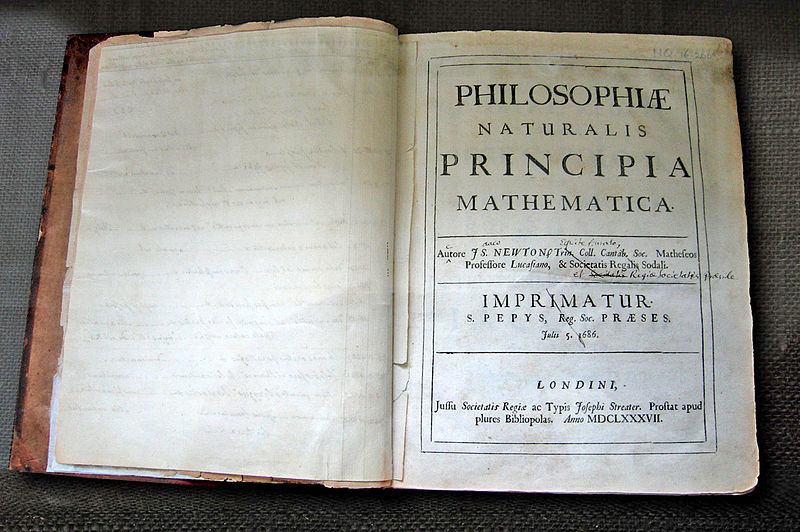
\includegraphics[width=1\textwidth]{./figures/horizontal_principia.png}
\caption{Fotografía de la copia persona de Newton de la primera edición
de los \emph{Principia}, incluyendo correcciones hechas a mano por el
mismo Newton. Foto: Andrew Dunn,
http://bit.ly/2WugALe.\label{fig:principia}}
\end{figure}
\end{quote}

\hypertarget{postulado_fuerzas}{%
\subsection{Postulado de fuerzas}\label{postulado_fuerzas}}

La manera original en la que Newton formuló sus postulados clásicos
sobre la relación entre las fuerzas aplicadas y el movimiento
resultante, ha cambiado mucho en los 350 años que nos separan de la
publicación de los \emph{Principia}. Hoy, existen maneras alternativas
de formular estos principios y leyes (algunas de las cuáles serán
desarrolladas en el libro) manteniendo los efectos prácticos de la
teoría.

A continuación usaremos una presentación de la mecánica newtoniana muy
propia del estilo de este libro y que sintetiza en un esquema formal,
sobre la base de los conceptos y cantidades definidas en las secciones
anteriores, sus postulados (leyes) y teoremas.
\begin{box_note}{Nota}

\textbf{Una formulación original.} El lector puede encontrar
relativamente extraña nuestra formulación (muy diferente a la que
encontrará en los textos de mecánica básica.) La razón de fondo estriba
esencialmente en la manera como hemos definido antes el concepto de
fuerza. Esta formulación sin embargo, como veremos a lo largo del libro,
además de contener los resultados básicos de la teoría conocidos por
todos, ofrece algunas ventajas para su formulación en teorías del
movimiento más general como la teoría de la relatividad.

\end{box_note}
La ley física en el corazón de la mecánica newtoniana se conoce como el
\textbf{postulado de fuerza}:
\begin{box_postulate}{Postulado}{box:pos:fuerzas}

\textbf{Postulado de Fuerzas.} Si en un sistema de referencia inercial,
una partícula esta sometida a una fuerza neta aplicada \(\vec F\) (suma
vectorial de las fuerzas aplicadas correspondientes a cada interacción
que sufre la partícula en ese instante) su momento lineal cambiará
instantáneamente a razón de:

\[
  \dot{p}=\vec F
  \]

En otros términos, la fuerza resultante es siempre igual la fuerza neta
aplicada:

\[ 
  \vec{\cal F}=\vec F
  \]

\end{box_postulate}
Aunque está última expresión parece obvia y universal, no lo es.
Recordemos que la fuerza aplicada \(\vec F\) es una propiedad de las
interacciones y su valor se cálcula a partir de los modelos epecíficos
que las describen. En contraposición, la fuerza resultante
\(\vec{\cal F}\) (la razón de cambio del momento lineal) es un efecto
observado en el movimiento de la partícula. El postulado fuerzas
básicamente plantea que en todas las interacciones a las que se somete
una partícula, la causa (fuerza aplicada) y el efecto (fuerza resultante
o razón de cambio del momento lineal) tienen el mismo valor.

Es importante resaltar la condición de que el sistema de referencia sea
inerical para que el postulado de fuerzas sea válido. En otras palabras,
en sistemas de referencia \emph{no} inerciales, la fuerza resultante no
es igual a la fuerza aplicada. Volveremos sobre este caso en la
\autoref{dinamica_rotantes}.

Por la suposición que hemos hecho desde el principio de que la masa de
las partículas es constante, el postulado de fuerzas nos permite
calcular la función de aceleración de las partículas que usamos en la
e.d.m. (ver Ec. \ref{eq:edm}). Si reconocemos que por definición para
una partícula \(\dot{\vec p}=m\vec a\), el postulado de fuerzas se puede
escribir como:

\[
\vec a = \frac{\vec F}{m}
\]

La e.d.m. de una partícula en función de las fuerzas aplicadas queda:

\begin{equation}
\label{eq:edm_fuerzas_aplicadas}
\ddot{\vec{r}}=\frac{\vec F}{m}.
\end{equation}
\begin{box_note}{Nota}

\textbf{Ecuación de movimiento con fuerzas resultantes.} Una relación
idéntica a la Ec. (\ref{eq:edm_fuerzas_aplicadas}) es válida en el caso
de las fuerzas resultandes:

\begin{equation}
  \label{eq:edm_fuerzas_resultantes}
  \ddot{\vec{r}}=\frac{\vec{\cal F}}{m}
  \end{equation}

Esta ecuación sin embargo no es un postulado de la mecánica, sino una
forma de la definición misma de fuerza aplicada \(\vec{\cal F}\) que
introdujimos en la \autoref{cantidades_dinamicas}.

Aunque la identidad matemática de las Ecs.
(\ref{eq:edm_fuerzas_aplicadas}) y (\ref{eq:edm_fuerzas_resultantes})
nos permite escribir la ecuación de movimiento sin distinguir que tipo
fuerzas están involucradas, no debemos olvidar la diferencia conceptual
entre una aceleración producto de las interacciones (fuerza aplicada,
Ec. \ref{eq:edm_fuerzas_aplicadas}) y aquella que es simplemente una
manifestación del cambio en el momento lineal (fuerza aplicada, Ec.
\ref{eq:edm_fuerzas_resultantes}).

\end{box_note}
La igualdad matemática, en sistemas inerciales, postulada entre la
fuerza neta aplicada sobre una partícula y la fuerza resultante, permite
extrapolar la definición de trabajo que presentamos en la
\autoref{cantidades_dinamicas} y derivar un importante teorema de la
mecánica newtoniana:
\begin{box_definition}{Proposición}{box:teo:trabajo.energia}

\textbf{Teorema del tabajo y la energía.} Si una partícula que en un
sistema de referencia inercial, se mueve sobre una trayectoria entre dos
puntos \(\vec r_1\) (donde tiene velocidad \(\vec v_1\)) y \(\vec r_2\)
(donde tiene velocidad \(\vec v_2\)), esta sometida a una fuerza neta
aplicada \(\vec F\) que cambia de acuerdo a una función conocida y
continua sobre la trayectoria, entonces, el trabajo realizado por la
fuerza aplicada es \(W = \int \vec{F}\cdot \mathrm{d}\vec r\) y la
siguiente igualdad es válida:

\[
  W = \Delta K
  \]

Donde \(K=mv^2/2\).

\end{box_definition}
\hypertarget{fuerzas_conservativas}{%
\subsection{Fuerzas conservativas y no
conservativas}\label{fuerzas_conservativas}}

Una clasificación adicional de las fuerzas (tanto resultantes como
aplicadas) surge al estudiar su \emph{circulación}
\(\oint \vec F \cdot d\vec r\) (ver \autoref{integrales}.) En
términos físicos, la circulación de una fuerza (resultante o aplicada)
es el trabajo total realizado por ella a lo largo de una trayectoria
cerrada.

De acuerdo con la circulación las fuerzas se clasifican en:

\begin{itemize}
\item
  \textbf{Fuerzas conservativas}: Una fuerza es conservativa si y solo
  sí, su circulación es nula:

  \begin{equation}
    \label{eq:circulacion_nula}
    \oint \vec F\cdot d\vec r=0
    \end{equation}

  Una manera más frecuente (y física) de expresar esta propiedad (ver
  problemas al final del capítulo) es diciendo que el trabajo realizado
  por una fuerza conservativa entre dos puntos del espacio, es
  independiente de la trayectoria que esta siga entre esos puntos.

  Por el teorema del tabajo y la energía, la circulación nula implica
  que la energía cinética de una partícula sometida a una fuerza
  conservativa, es la misma antes y después de recorrer una trayectoria
  cerrada. Este es precisamente el origen del adjetivo
  \emph{conservativo}.
\end{itemize}

\begin{itemize}
\tightlist
\item
  \textbf{Fuerzas no conservativas o disipativas}: Una fuerza es
  \emph{no} conservativa si su circulación es distinta de cero. En este
  caso, en virtud del teorema del trabajo y la energía, la energía
  cinética de la partícula antes y después de realizar el recorrido
  cerrado, será diferente. Es por esta razón que a este tipo de fuerzas
  se las llama también \emph{fuerzas disipativas}.
\end{itemize}
\begin{box_note}{Nota}

\textbf{La fuerza como campo vectorial.} Nótese que al definir la
circulación o al hablar aquí del trabajo realizado sin importar el
camino seguido por la partícula, estamos asumiendo que en todos los
puntos del espacio a los que tiene acceso la partícula, podemos calcular
el valor de la fuerza \(\vec F\). En este sentido la fuerza ya no es
simplemente un vector más, sino que se convierte en lo que en el cálculo
se conoce como un \emph{campo vectorial}, es decir, una función que
asocia a cada punto del espacio un vector (ver \autoref{funciones}.)

\end{box_note}
La propiedad expresada en la Ec. (\ref{eq:circulacion_nula}) implica,
por el corolario al teorema de Stokes (Cor. \ref{box:cor:stokes}) que
las fuerzas conservativas se pueden escribir como:

\begin{equation}
\label{eq:funcion_energia_potencial}
\vec F = -\vec{\nabla} U = -\partial_{\vec r} U
\end{equation} donde el signo menos, que parece arbitrario, es una
convención usada frecuentemente en física (y que se justificará en la
siguiente sección.)

En mecánica llamamos a \(U\) la \textbf{función de energía potencial} de
la fuerza conservativa.

Las fuerzas conservativas pueden describirse o bien usando un campo
escalar \(U\) (el campo de energía portencial) o bien usando un campo
vectorial \(\vec F\) (como se acostumbra con todas las fuerzas,
conservativas o no). El uso de una descripción o de la otra dependerá de
la situación que estemos considerando.

\hypertarget{energia_mecanica}{%
\subsection{Energía mecánica}\label{energia_mecanica}}

Con la definición de la función de energía potencial, el trabajo
realizado por una fuerza conservativa se puede escribir como:

\begin{eqnarray}
\int \vec F\cdot \mathrm{d}\vec r & = & -\int \partial_{\vec r} U \cdot \mathrm{d}\vec r\nonumber\\
& = & -\int \mathrm{d}\mathrm{U}\nonumber\\
& = & -[U(\vec r_2)-U(\vec r_1)]\nonumber\\
& = & -\Delta U\nonumber
\end{eqnarray} donde hemos usado, en su orden, la regla de la cadena
(Teo. \ref{box:teo:regla.cadena}) y la rela de Newton-Leibniz (Teo.
\ref{box:teo:regla.newton.leibniz}).

El teorema del trabajo y la energía (Teo. \ref{box:teo:trabajo_energia})
para una fuerza conservativa se escribe entonces como:

\begin{equation}
\label{eq:deltaU_deltaK}
\begin{array}{rcl}
-\Delta U & = & \Delta K\\
\Delta(K+U) & = & 0.
\end{array}
\end{equation}

Este último resultado implica que la cantidad \(E\equiv K+U\) se
conserva durante el movimiento de una partícula bajo la acción de una
fuerza conservativa. Llamaremos a esta cantidad en lo sucesivo
\textbf{energía mecánica} y a esta interesante propiedad (que es
producto del teorema del trabajo y la energía), \textbf{conservación de
la energía mecánica}.

El resultado anterior puede generalizarse cuando sobre la partícula
actúan todo tipo de fuerzas, aplicadas o resultantes, conservativas o no
conservativas:
\begin{box_theorem}{Proposición}{box:teo:conservacion.energia}

\textbf{Conservación de la energía.} Si una partícula se mueve en el
espacio mientras esta sometida a fuerzas conservativas y no
conservativas, el trabajo total realizado por las fuerzas no
conservativas \(W_{\rm NC}\) entre dos puntos cualquiera de la
trayectoria es:

\[
W_\mathrm{NC} = \Delta E
\]

Donde \(E\equiv K+\sum U_i\), siendo \(\{U_i\}\) las funciones de
energía potencial asociadas a todas las fuerza conservativas que actúan
sobre la partícula. Llamamos a \(E\) la energía mecánica total de la
partícula.

\end{box_theorem}
\hypertarget{ley_inercia}{%
\subsection{¿Ley de inercia?}\label{ley_inercia}}

En la historia de la mecánica, el concepto de \emph{inercia} o
\emph{movimiento inercial}, y la \emph{ley de inercia} de Newton,
jugaron un papel fundamental en la ruptura con los conceptos dinámicos
de la física Aristótelica que postulaban que todo movimiento necesitaba
una \emph{causa motriz} (una \emph{fuerza aplicada} en nuestro caso.)

En los Principia y en sus reformulaciones posteriores
\cite{Chandrasekhar2003Principia}, la inercia aparece postulada como la
primera ley movimiento.

En el esquema con el que hemos sintetizado la mecánica newtoniana aquí,
la inercia no tiene que postularse, sino que en realidad es un teorema
muy sencillo que se sigue (casi trivialmente) del postulado de fuerzas:
\begin{box_theorem}{Proposición}{box:teo:inercia}

\textbf{Teorema de inercia.} Si la fuerza resultante o la fuerza neta
aplicada sobre una partícula es nula durante un cierto intervalo de
tiempo \([t_1,t_2)\)\footnote{El intervalo es cerrado en \(t_1\) en
  tanto en algún momento tiene que comenzar la condición de movimiento
  libre de fuerzas, mientras que es abierto en \(t_2\) en tanto esa
  condición podría extenderse para siempre}, su momento lineal en ese
intervalo será constante e igual al momento lineal que tenía en \(t_1\):

\[
   \vec F(t\in[t_1,t_2))=\vec 0\Longleftrightarrow \vec p(t\in[t_1,t_2))=\vec{p}(t_1)
   \]

En otras palabras durante el intervalo considerado la partícula estará
en reposo (si \(\vec p(t_1)=\vec 0\)) se moverá siguiendo una
trayectoria rectilínea y con velocidad constante
\(\vec v=\vec p(t_1)/m\).

\end{box_theorem}
\hypertarget{postulado_accion_reaccion}{%
\subsection{Postulado de acción y
reacción}\label{postulado_accion_reaccion}}
\begin{box_postulate}{Postulado}{box:pos:accion.reaccion}

\textbf{Acción y reacción.} En un sistema de referencia inercial en el
que dos partículas 1 y 2 interactúan mutuamente, sea a través de fuerzas
de contacto o de campo, se cumple que:

\begin{itemize}
\tightlist
\item
  (\textbf{Forma débil del postulado de acción y reacción}) la fuerza
  \(\vec{F}_{12}\) que la partícula 1 experimenta por la interacción con
  la partícula 2 (que llamaremos \emph{acción}), es igual pero de
  sentido contrario a la fuerza \(\vec{F}_{21}\) que la partícula 2
  experimenta por la interacción con la partícula 1 (que llamaremos
  \emph{reacción}; ver panel izquierdo de la
  \autoref{fig:accion_reaccion}.)
\end{itemize}

o bien,

\begin{itemize}
\tightlist
\item
  (\textbf{Forma fuerte de la ley de acción y reacción}) las fuerzas de
  acción y reacción, definidas arriba, son además paralelas a la línea
  que une las posiciones de las partículas (ver panel derecho de la
  \autoref{fig:accion_reaccion}).
\end{itemize}

\end{box_postulate}
\begin{figure}[t!]
\centering
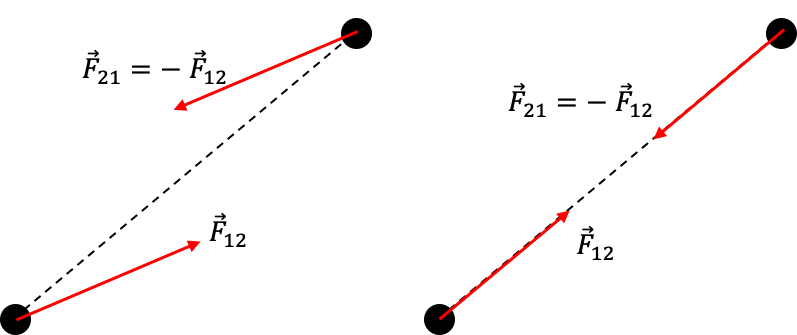
\includegraphics[width=0.8\textwidth]{./figures/horizontal_accion_reaccion.png}
\caption{Dos formas del postulado de acción y reacción: a la izquierda
el postulado débil, en el que las fuerzas son iguales y de sentido
contrario, pero no son paralelas a la línea que une las partículas; a la
derecha el postulado fuerte en el que la acción y reacción actúan sobre
la línea que une a las
partículas.\label{fig:accion_reaccion}}
\end{figure}

Las consecuencias de este postulado son fundamentales en la mecánica y
serán discutidas en la \autoref{dinamica_sistemas}.

\hypertarget{postulado_gravitacion}{%
\subsection{Postulado de gravitación
universal}\label{postulado_gravitacion}}

Una de los más atrevidos y visionarios postulados de Newton sobre la
naturaleza del movimiento de los cuerpos y en general del Universo, se
conoce como la \textbf{ley o postulado de gravitación universal} que en
su forma moderna propone:
\begin{box_postulate}{}{box:pos:gravitacion.universal}

\begin{quote}
\textbf{Postulado de gravitación universal}. Una partícula de masa
\(m_1\) situada en \(\vec r_1\) ejerce sobre cualquier otra partícula de
masa \(m_2\) situada en un \(\vec r_2\), una fuerza instantánea a
distancia dada por:
\end{quote}

\[
\vec F=-\frac{G m_1 m_2}{r^2}\hat r
\]

\begin{quote}
donde \(\vec r\equiv\vec r_2-\vec r_1\) y
\(G=6.67408(31)\times 10^{-11}\) m\(^3\) kg\(^{-1}\) s\(^{-2}\)
\(=(6.67408\pm 0.00031)\times 10^{-11}\) m\(^3\) kg\(^{-1}\) s\(^{-2}\)
es una constante de la naturaleza conocida como la \emph{constante de
gravitación universal} o \emph{constante de Cavendish}.
\end{quote}

\end{box_postulate}
En lo sucesivo usaremos la notación más precisa y consistente (ver
\autoref{fig:fuerza_gravitacional}):

\begin{equation}
\label{eq:fuerza_gravitacional}
\vec F_{12}=-\frac{G m_1 m_2}{r_{12}^3}\vec{r}_{12}
\end{equation}

Donde \(\vec{r}_{12}\equiv\vec{r}_1-\vec{r}_2\).

Nótese que esta forma del postulado de gravitación universal, ofrece una
expresión para la fuerza \emph{sobre} la partícula 1 en lugar de la que
ella ejerce sobre la partícula 2 (aunque por el postulado de acción y
reacción son iguales). Además, el vector relativo \(\vec{r}_{12}\) (ver
\autoref{fig:fuerza_gravitacional}) va de la partícula 2 a la partícula
1 (en lugar de \(\vec r\) que en el enunciado del postulado que va de la
1 a la 2). Asegúrese de entender claramente la definición y el sentido
de estos vectores que serán usados con mucha frecuencia a lo largo del
texto.

\begin{figure}[t!]
\centering
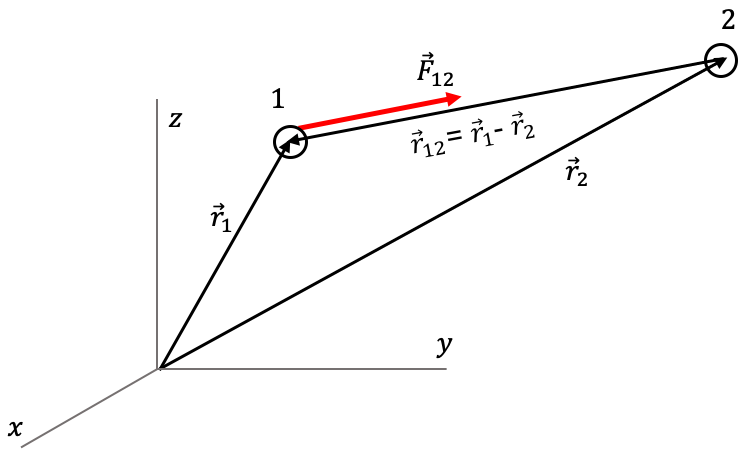
\includegraphics[width=0.8\textwidth]{./figures/horizontal_fuerza_gravitacional.png}
\caption{Definición de los vectores de posición, vector relativo y
vector de fuerza en el postulado de gravitación
universal.\label{fig:fuerza_gravitacional}}
\end{figure}
\begin{box_note}{Nota}

\textbf{La fuerza de gravedad y la ley de acción y reacción.} Como puede
verse de la definición matemática de la fuerza de gravitación (Ec.
\ref{eq:fuerza_gravitacional}), tanto ella como su reacción, satisfacen
las condiciones del postulado fuerte de acción y reacción, lo que tendrá
consecuencias fundamentales cuando estudiemos las simetrías y cantidades
conservadas en sistemas de varias partículas interactuando
gravitacionalmente.

\end{box_note}
\hypertarget{fuerza_luna}{%
\subsection{La fuerza gravitacional de la Tierra, el Sol y la la
Luna}\label{fuerza_luna}}

Para poner en un contexto práctico las ideas de la sección anterior,
calcularemos aquí la fuerza gravitacional ejercida por el Sol y la
Tierra sobre la Luna.

Si bien el postulado de gravitación universal (Ec.
\ref{eq:fuerza_gravitacional}), aplica solamente para partículas
puntuales, como se explico desde el principio, dadas las dimensiones del
Sistema Solar, podemos asumir que los tres cuerpos en cuestión son muy
pequeños.

El cálculo de la Fuerza requiere que compilemos primero la información
sobre las masas y distancias de estos cuerpos:

    \begin{code}{}{}\begin{Verbatim}[fontsize=\small,commandchars=\\\{\}]
\PY{c+c1}{\PYZsh{} Constante de gravitación}
\PY{n}{G}\PY{o}{=}\PY{l+m+mf}{6.67408e\PYZhy{}11} \PY{c+c1}{\PYZsh{}m\PYZca{}3/kg s\PYZca{}2}

\PY{c+c1}{\PYZsh{}Masa de los cuerpos}
\PY{n}{M\PYZus{}tierra}\PY{o}{=}\PY{l+m+mf}{5.97e24} \PY{c+c1}{\PYZsh{}kg}
\PY{n}{M\PYZus{}luna}\PY{o}{=}\PY{l+m+mf}{7.34e22} \PY{c+c1}{\PYZsh{}kg}
\PY{n}{M\PYZus{}sol}\PY{o}{=}\PY{l+m+mf}{1.98e30} \PY{c+c1}{\PYZsh{}kg }

\PY{c+c1}{\PYZsh{}Distancia entre ellos}
\PY{n}{d\PYZus{}sol\PYZus{}tierra}\PY{o}{=}\PY{l+m+mi}{149600000}\PY{o}{*}\PY{l+m+mi}{1000} \PY{c+c1}{\PYZsh{}m}
\PY{n}{d\PYZus{}tierra\PYZus{}luna}\PY{o}{=}\PY{l+m+mi}{385000}\PY{o}{*}\PY{l+m+mi}{1000} \PY{c+c1}{\PYZsh{}m}
\PY{n}{d\PYZus{}sol\PYZus{}luna}\PY{o}{=}\PY{n}{d\PYZus{}sol\PYZus{}tierra}\PY{o}{\PYZhy{}}\PY{n}{d\PYZus{}tierra\PYZus{}luna}
\end{Verbatim}

%%

\end{code}

Aunque la distancia entre el Sol y la Luna cambia continuamente debido
al complejo movimiento de nuestro satélite, asumiremos, para nuestro
sencillo cálculo, la mínima distancia entre ellos, es decir la distancia
a la que se encuentran en la fase de Luna Nueva (cuando la Luna esta
entre la Tierra y el Sol.)

Las fuerzas entre ellos serán por tanto:

    \begin{code}{}{}\begin{Verbatim}[fontsize=\small,commandchars=\\\{\}]
\PY{n}{F\PYZus{}sol\PYZus{}tierra}\PY{o}{=}\PY{n}{G}\PY{o}{*}\PY{n}{M\PYZus{}sol}\PY{o}{*}\PY{n}{M\PYZus{}tierra}\PY{o}{/}\PY{n}{d\PYZus{}sol\PYZus{}tierra}\PY{o}{*}\PY{o}{*}\PY{l+m+mi}{2}

\PY{n}{F\PYZus{}sol\PYZus{}luna}\PY{o}{=}\PY{n}{G}\PY{o}{*}\PY{n}{M\PYZus{}sol}\PY{o}{*}\PY{n}{M\PYZus{}luna}\PY{o}{/}\PY{n}{d\PYZus{}sol\PYZus{}luna}\PY{o}{*}\PY{o}{*}\PY{l+m+mi}{2}

\PY{n}{F\PYZus{}tierra\PYZus{}luna}\PY{o}{=}\PY{n}{G}\PY{o}{*}\PY{n}{M\PYZus{}tierra}\PY{o}{*}\PY{n}{M\PYZus{}luna}\PY{o}{/}\PY{n}{d\PYZus{}tierra\PYZus{}luna}\PY{o}{*}\PY{o}{*}\PY{l+m+mi}{2}
\end{Verbatim}

%%

\end{code}
\vspace{-1em}

%%hidecode


    \begin{Verbatim}[fontsize=\small,commandchars=\\\{\}]
F\_sol\_tierra = 3.525069974834854e+22 N 
F\_sol\_luna = 4.356399422118894e+20 N 
F\_tierra\_luna = 1.9730602178040146e+20 N 
\end{Verbatim}

Si bien, fuerzas tan grandes son difíciles de interpretar en términos
cotidianos (la fuerza gravitacional que ejerce la Tierra sobre una
persona con una masa de 60 kg es de apenas 590 N), un hecho
``inesperado'' llama la atención: la fuerza que ejerce el Sol sobre la
Luna es más del doble que la que ejerce la Tierra sobre ella. ¿Será
porque usamos la distancia de la Luna en la fase de nueva cuando está
más cerca al Sol? ¿cuanto disminuirá la fuerza del Sol sobre la Luna si
la ponemos en una posición cercana la fase de Luna Llena? ¿a qué
distancia debería estar la Luna de la Tierra para que la fuerza de
nuestro planeta sobre la primera igualará a la que siente del Sol?
¿órbita entonces la Luna al Sol o a la Tierra? y si ese es el caso ¿por
qué la hemos considerado siempre nuestro ``satélite''?

Dejamos al lector la discusión y solución de estas preguntas (algunas de
las cuáles serán ampliadas en la sección de problemas al final del
capítulo), pero no podemos dejar de mencionar que una importante
motivación para los desarrollos de la mecánica celeste posteriores a los
tiempos de Newton, fue precisamente resolver la última de esas
preguntas. Volveremos a este asunto en un capítulo posterior.
\begin{box_history}{Un poco de historia}{}{nofloat}
\small

\textbf{Hooke y el postulado de gravitación.} Si bien Newton es
recordado por ser el padre intelectual de la teoría de gravitación
universal, una de sus contribuciones fundamentales a la física y el
punto de partida de la mecánica celeste moderna, la idea de que el
movimiento de los planetas se debía a una fuerza dirigida hacia el Sol
(no hacia adelante en sus órbitas, como habían propuesto Kepler y
Descartes) fue presentada por primera vez ante la Royal Society por
Robert Hooke (``huk'', ver \autoref{fig:hooke}).

En 1666 (el mismo año en el que un Newton de 22 años, recién graduado,
comenzaba sus propias reflexiones sobre el fenómeno gravitacional sin
comunicarselo a nadie), Hooke escribió:

\begin{quote}
``\emph{Explicaré un sistema del mundo que difiere en muchos
particulares de cualquier otro conocido hasta ahora {[}\ldots{}{]} Este
sistema depende de tres supuestos. Primero, que todos los cuerpos
celestes posean un poder atractivo o gravitatorio hacia sus propios
centros, de modo que no tan solo a sus partes, impidiendo que se alejen
de ellos, como observamos hace la Tierra, sino que también atraigan a
todos los demás cuerpos celestes que hallen dentro de su zona de
actividad {[}\ldots{}{]} La segunda suposición es que todos los cuerpos
que son puestos en movimiento simple y directo continúen moviéndose
hacia delante en una línea recta, hasta que se encuentre con alguna otra
fuerza efective que los desvíe e incline en un movimiento que describa
un círculo, una elipse o cualquier otra línea curva compuesta. La
tercera suposición es que esas fuerzas de atracción sean tanto más
poderosas en su acción cuanto el cuerpo que debe snetri su influencia se
halle más cerca de su centro.}'' \cite{Christianson1984Newton}
\end{quote}

Como puede leerse en este extracto, en los escritos de Hooke, que a
diferencia de Newton no desarrollo mucho más allá de esta sencilla
formulación, estaba la semilla no solo de la idea de la gravedad, sino
que también se presentaba una versión de la ley de inercia y el
principio de disminución de la intensidad gravitacional con la
distancia. Más adelante Hooke iría más lejos y propondría que la
intensidad de la fuerza disminuía específicamente con el cuadrado del
inverso de la distancia, en una carta dirigida a Newto y fechada en
enero de 1680.

Después de que Newton presentará en sus escritos de esa misma década de
1680, incluyendo los \emph{Principia}, su postulado de gravitación
universal, comenzó con Hooke una penosa disputa de prioridad. Hooke
acuso a Newton hasta su muerte de haberle robado las ideas de la
gravitación universal y Newton despreció profundamente Hooke por sugerir
que su contribución más grande a la historia de la ciencia había sido
copiada de otro. Hoy la historia le reconoce a Hooke su prioridad (o al
menos simultaneidad) en dos ideas: la idea de la atracción universal
(que concibió simultaneamente e independeintemente con Newton) y la idea
(planteada como una hipótesis sin demostración matemática) de que los
cuerpos sometidos a una fuerza gravitacional se mueven sobre elipses, un
asunto sobre el que volveremos en el \autoref{problema_doscuerpos}.

\end{box_history}
\begin{figure}[tb!]
\centering
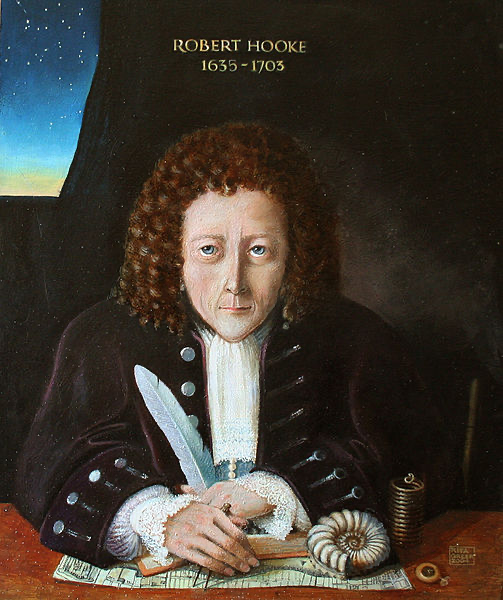
\includegraphics[width=0.5\textwidth]{./figures/vertical_robert_hooke.png}
\caption{Robert Hooke (1635-1753). Crédito: Rita Greer
(2004).\label{fig:hooke}}
\end{figure}

\hypertarget{campo_gravitacional}{%
\subsection{El campo gravitacional}\label{campo_gravitacional}}

Otra forma de escribir el postulado de gravitación, es reconcer que la
fuerza gravitacional que produce una partícula de masa \(M\) sobre
cualquier otra partícula de masa \(m\) situada en un punto arbitrario
con posición relativa \(\vec r\) (donde \(\vec r\) es el vector que va
de la posición de \(M\) a la del punto arbitratio) es:

\begin{equation}
\label{eq:fuerza_M_m}
\vec F=m\left(-\frac{GM}{r^3}{\vec r}\right)
\end{equation}

De aquí podemos postular que el \emph{campo vectorial}:

\begin{equation}
\label{eq:campo_gravitacional}
\vec g\equiv-\frac{GM}{r^3}{\vec r},
\end{equation} \emph{existe} independiente de si hay una masa \(m\) que
pueda sentirlo. A esta cantidad vectorial (¿entidad física?) la
llamaremos en lo sucesivo el \textbf{campo gravitacional} producido por
la partícula puntual \(M\).

En términos del campo gravitacional, la fuerza que experimenta una
partícula de prueba situada en \(\vec r\) respecto a \(M\) se escribe:

\begin{equation}
\label{eq:fuerza_campo_gravitacional}
\vec F=m\vec g
\end{equation}

Esta última relación esta lejos de ser trivial. En realidad la
extenderemos para denotar, de manera general, la fuerza gravitacional
experimentada por una partícula en un campo gravitacional \(\vec g\),
independientemente de si el campo es producido por una partícula
puntual, por un sistema de partículas, un cuerpo rígido o un fluído.

\hypertarget{energia_potencial_gravitacional}{%
\subsection{Energía potencial
gravitacional}\label{energia_potencial_gravitacional}}

Es posible demostrar (ver problemas al final de este capítulo) que la
fuerza gravitacional de la Ec. (\ref{eq:fuerza_M_m}), es una fuerza
conservativa con función de energía potencial igual a:

\begin{equation}
\label{eq:energia_potencial_gravitacional}
U=-\frac{G M m}{r},
\end{equation}
\begin{box_note}{Nota}

\textbf{Energía potencial gravitacional negativa.} En términos rigurosos
la función de energía potencial más general de la que podemos derivar la
fuerza gravitacional es

\[U=-\frac{GMm}{r}+C\]

siendo \(C\) una constante arbitraria. Esta libertad implica que el
valor de la energía gravitacional no tiene en realidad un significado
físico relevante. Lo importante en la dinámica es la diferencia de
energía potencial entre dos puntos del espacio \(\Delta U\) y que
determina, por ejemplo, el cambio en la energía cinética a través de la
Ec. (\ref{eq:deltaU_deltaK}.) Naturalmente para el cáluclo de
\(\Delta U\) el valor de \(C\) es irrelevante.

La elección arbitraria de \(C=0\) que hicimos al escribir la Ec.
(\ref{eq:energia_potencial_gravitacional}), sin embargo, tiene una
interpretación interesante, que podemos obtener al aplicar la
conservación de la energía \(\Delta K=-\Delta U\) en una situación
hipotética.

Imaginemos que cuando dos partículas están a una distancia \(r\) finita,
su energía cinética total es 0 (están en reposo relativo) y su energía
potencial \(U_0<0\). Por efecto de la acción instantánea de un agente
externo, una de las partículas se acelera (el sistema recibe una
inyección de energía mecánica \(\Delta E>0\)) hasta que las dos
partículas terminan separadadas a una distancia enorme
\(r\rightarrow \infty\) donde su velocidad vuelve a ser casi nula
\(v\rightarrow 0\) (podría ser mayor, pero asumiremos este caso
extremo).

A esa distancia, el sistema tiene energía cinética total
\(K\rightarrow0\) y dado que \(C=0\), su energía potencial será también
\(U\rightarrow 0\). Aplicando la conservación de la energía mecánica
total:

\[
  \begin{array}{rcl}
  \Delta K & = & -\Delta U\\
  0-(0+\Delta E) & = & -(0-U_0)\\
  \Delta E & = & -U_0
  \end{array}
  \]

En conclusión: \emph{El valor absoluto de la energía potencial \(U_0\)
se puede interpretar como la energía mecánica adicional que necesita un
sistema para apenas escapar de su mutua interacción gravitacional}.

En otros términos, el signo negativo de la energía potencial podría
interpretarse no solamente como una elección arbitraria de una constante
matemática sino también como una \emph{deuda energética}, es decir como
la energía que debe aportar un agente externo para liberar a las
partículas de su ``esclavitud'' gravitacional.

\end{box_note}
Dado que la energía potencial de cualquier partícula, sometida a la
fuerza gravitacional de \(M\) es proporcional a su masa \(m\), es
posible definir la \textbf{función de potencial gravitacional} o
simplemente el \textbf{potencial gravitacional}:

\begin{equation}
\label{eq:campo_gravitacional}
V \equiv \frac{U}{m} = -\frac{GM}{r}
\end{equation}

\(V\) es un campo escalar (de acuerdo a las definiciones de
\autoref{funciones}) y como sucede con el campo vectorial
\(\vec g\), en muchas aplicaciones es la representación matemática del
\emph{campo gravitacional} producido por una partícula.
En términos de $V$, la energía potencial de una partícula de masa $m$ sumergida en un campo gravitacional y la fuerza experimentada por ella, se pueden escribir como:

\begin{equation}
\label{eq:energia_fuerza_campo_gravitacional}
\begin{array}{rcl}
U & = & m V \\
\vec F & = & -m\;\partial_{\vec r} V
\end{array}
\end{equation}

De nuevo, junto con la Ec. (\ref{eq:fuerza_campo_gravitacional}) estas relaciones aplican, independientemente de si el campo gravitacional, cuantificado por $V$ o $\vec g$, es producido por una partícula o un cuerpo extendido.
Una última relación interesante que resulta de comparar la Ec.
(\ref{eq:energia_fuerza_campo_gravitacional}) con la Ec.
(\ref{eq:fuerza_campo_gravitacional}) es la siguiente:

\begin{equation}
\label{eq:potencial_campo_gravitacional}
\vec g  = -\partial_{\vec r} V
\end{equation} que es análoga a la definición de \(U\) (ver Ec.
\ref{eq:funcion_energia_potencial}), \(\vec F=-\partial_{\vec r} U\).

\hypertarget{masa_equivalencia}{%
\subsection{Masa y principio de equivalencia}\label{masa_equivalencia}}

La masa, como aparece en la Ec. (\ref{eq:campo_gravitacional}), es tanto
una medida de las capacidad de un cuerpo para producir campo
gravitacional (y afectar a otras partículas), o, como se expresa en
\ref{eq:fuerza_campo_gravitacional}, una medida de su ``sensibilidad''
al campo gravitacional producido por otros cuerpos \footnote{En términos
  estrictos, la masa que produce el campo y la masa que lo siente,
  deberían diferenciarse también. La primera sería una masa
  gravitacional activa y la segunda una masa gravitacional pasiva. En lo
  que sigue nos ocuparemos únicamente de la masa gravitacional pasiva, o
  para acortar, la masa gravitacional.}.

La masa, así concebida, es muy diferente, conceptualmente, a la que
usamos (y uso Newton originalmente) para definir las cantidades
dinámicas en la \autoref{cantidades_dinamicas}. Por ello es
necesario precisar la diferencia entre esos dos tipos de masa con una
definición:
\begin{box_definition}{Definición}{box:def:masas}

\textbf{Masa inercial y masa gravitacional.} En mecánica Newtoniana
distinguimos dos tipos de masa conceptualmente diferentes:

Llamamos \textbf{masa inercial m\_I} a la razón entre las magnitudes del
momento lineal de una partícula y su velocidad, a saber \(m_I=p/v\). La
masa inercial de una partícula es la que aparece en la ecuación de
movimiento \(\ddot{\vec{r}}=\vec F/m_I\) y en la energía cinética
\(K=m_I v^2/2\).

Por otro lado la \textbf{masa gravitacional \(m_G\)} es la masa que
determina la intensidad del campo gravitacional producido por una
partícula \(V=G m_G/r\) (\emph{masa gravitacional activa}) \emph{o} la
intensidad de la fuerza que ella experimenta en un campo gravitacional
de otro cuerpo, \(\vec F=m_G\vec g\) (\emph{masa gravitacional pasiva}).

\end{box_definition}
Si usamos el postulado de fuerza (Ec. \ref{eq:edm_fuerza_aplicadas}) y
la expresión para la fuerza gravitacional escrita en la Ec.
(\ref{eq:fuerza_campo_gravitacional}), encontramos que la aceleración
que sufre una partícula de masa inercial \(m_I\) y masa gravitacional
(pasiva) \(m_G\) en un campo gravitacional \(\vec g\) es:

\begin{equation}
\label{eq:razon_masa_gravitacional_masa_inercial}
\ddot{\vec r}=\frac{m_G}{m_I}\vec g
\end{equation}

La razón \(m_G/m_I\), ha sido medida cuidadosamente en el laboratorio
desde finales del siglo 1500 (ver recuadro \textbf{Un poco de historia:
El experimento de Eötvos}), con un resultado ampliamente conocido: el
valor numérico de la masa gravitacional (pasiva) coincide con el de la
masa inercial hasta la onceava cifra significativa
\cite{Roll1964Equivalence}.

La igualdad entre la masa gravitacional e inercial ha sido elevada hoy a
la altura de un principio fundamental de la mecánica, el
\textbf{principio de equivalencia}:
\begin{box_principle}{Principio}{box:pri:equivalencia}

\textbf{Principio de equivalencia (versión débil).} \footnote{El
  adjetivo débil, hace referencia al hecho de que existe un principio de
  equivalencia más fundamental sobre el que se sustenta la teoría de la
  relatividad general.}. La aceleración de de una partícula puntual en
un campo gravitacional depende únicamente del valor del campo y es
independiente de la masa y composición de la partícula. En términos
matemáticos, en la mecánica newtoniana, \(m_G=m_I\).

\end{box_principle}
Por la igualdad numérica (mas no conceptual) entre la masa gravitacional
(pasiva) y la mas inercial, en el contexto de la mecánica newtoniana,
usaremos en lo sucesivo el símbolo \(m\) para referirnos a la masa sin
distinguir si se trata de la una o la otra.
\begin{box_history}{Un poco de historia}{}{nofloat}
\small

\textbf{El experimento de Eötvos.} La pregunta de sí dos cuerpos de
distinta masa caen al mismo tiempo cuando son lanzadas desde la misma
altura (que, en términos modernos, es igual a la pregunta de si tienen
la misma aceleración), ha ocupado a pensadores desde la antigüedad.

El primer experimento preciso de este tipo fue realizado por Simon
Stevin (1548-1620, ver \autoref{fig:stevin}), un matemático, filósofo e
ingeniero \emph{flamenco} (es decir de la región que hoy llamamos
Bélgica) que hizo importantes contribuciones tempranas a la mecánica
prenewtoniana.

En 1586, Stevin lanzó dos esferas de acero que tenían una masa diferente
por un factor de 10, desde una altura de aproximadamente 10 metros.
Registro la diferencia en el tiempo de caída escuchando el golpe que
hacían las esferas al golpear el suelo \cite{Devreese2008Stevin}. El
resultado fue contundente: las dos esferas caían casi exactamente al
mismo tiempo (al menos dentro de la sensibilidad del experimento.)

Posteriormente Galileo (quien citaría a Stevin en sus libros) realizó
comprobaciones similares usando planos inclinados \footnote{La idea de
  que Galileo realizó un experimento similar al de Stevin, lanzando
  objetos desde lo alto de la Torre de Pisa no ha podido ser confirmado
  y podría tratarse de una anécdota apócrifa.}. Newton y Bessel
intentaron resolver también la cuestión, esta vez usando péndulos (el
período de un péndulo depende también de la aceleración que sufre el
cuerpo) con resultados similares a Stevin: todos los cuerpos sin
importar su masa y composición, tienen la misma aceleración en el campo
gravitacional de la Tierra. En términos de la Ec.
(\ref{eq:razon_masa_gravitacional_masa_inercial}), \(m_G/m_I=1\).

Las medidas más precisas de la razón entre las masas gravitacional e
inercial fueron realizadas entre 1889 y 1909 por el físico húngaro
Roland von Eötvos
(\hreffoot{https://es.forvo.com/search/E\%C3\%B6tv\%C3\%B6s/hu/}{``fon
otfosh''}) y sus colaboradores, usando para ello un instrumento conocido
como la balanza de torsión (similar al usado para medir la constante de
gravitación universal.) Los experimentos probaron la igualdad entre la
masa gravitacional y la masa inercial hasta la octava cifra
significativa y fueron repetidos en la segunda mitad de los 1900 hasta
alcanzar la precisión mencionada en el texto: once dígitos
significativos \cite{Roll1964Equivalence}.

\end{box_history}
\begin{quote}
\begin{figure}[tb!]
\centering
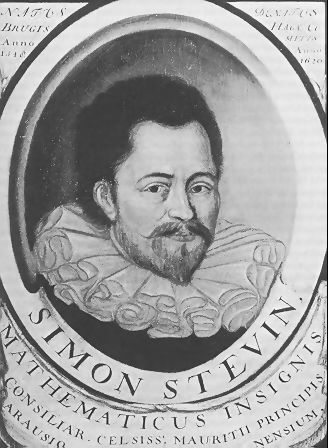
\includegraphics[width=0.5\textwidth]{./figures/vertical_simon_stevin.png}
\caption{El único retrato disponible de Simon Stevin (ca. 1548).
Crédito: Colección Universidad de Leiden.\label{fig:stevin}}
\end{figure}
\end{quote}



\hypertarget{sistemas_particulas}{%
\section{Sistemas de partículas}\label{sistemas_particulas}}

Una vez definidas las cantidades y conceptos básicos de la mecánica y
formulados los principios, postulados y teoremas que nos permiten
describir el movimiento de partículas puntuales, tenemos los elementos
necesarios para abordar la cinemática y dinámica de sistemas formados
por muchas partículas.

Los sistemas considerados aquí, sin embargo, estarán constituidos por
partículas que interactúan a distancia, con fuerzas relativamente
débiles y en números relativamente pequeños. La mecánica de sistemas con
partículas unidas por fuerzas intensas y que mantienen su posición
relativa de forma estable (cuerpos rígidos) o aquellos formados por
\emph{moles} de partículas individuales, y cuya mecánica es descrita por
leyes empíricas macroscópicas o por reglas estadística, está más allá
del interés del libro.

Una buena parte de los desarrollos teóricos contenidos en esta sección
vienen originalmente del texto clásico de Goldstein, Poole \& Safko,
``\emph{Classical mechanics}'' \cite{Goldstein2002} y que estaremos
citando con alguna frecuencia en el resto de este libro.

\hypertarget{fuerzas_centro_masa}{%
\subsection{Fuerzas y centro de masa}\label{fuerzas_centro_masa}}

Cada partícula en nuestro sistema esta sometida a dos tipos de fuerzas:
(1) las fuerzas externas \(\vec{F}^{E}_i\), producidas por cuerpos
externos o campos diferentes a los producidos por las componentes del
sistema y (2) las fuerzas entre las partículas \(\vec{F}_{ij}\).

La evolución del sistema se obtiene resolviendo simultáneamenete el
conjunto de las e.d.m. de cada partícula, que se puede escribir en
términos de las fuerzas externas e internas como:

\begin{equation}
\label{eq:edm_sistema_particulas}
\left\{m_i \ddot{\vec r_i} = \vec F^E_i+\sum_{j\neq i} \vec F_{ij}\right\}_N
\end{equation}

Si sumamos todas las e.d.m. y suponemos que las fuerzas entre partículas
satisfacen la ley de acción y reacción (débil o fuerte), esto es
\(\vec{F}_{ji}=-\vec{F}_{ij}\), podemos escribir:

\[
\sum_i m_i \ddot{\vec r_i} = \sum_i \vec F^E_i
\] o bien:

\[
\frac{\mathrm{d}^2}{\mathrm{d}t^2}\left(\sum_i m_i \vec{r}_i\right) = \sum_i \vec F^E_i
\]

Si definimos:

\begin{equation}
\label{eq:centro_masa}
\vec R\equiv \frac{\sum_i m_i \vec{r}_i}{M}
\end{equation} donde \(M=\sum_i m_i\) es la masa total del sistema, las
e.d.m. de todas las partículas del sistema se transforman en una sola
ecuación, que tiene exactamente la misma forma que la e.d.m. de una sola
partícula de masa \(M\) y posición \(\vec{R}\) sometida a una fuerza
total \(F^E=\sum_i \vec F^E_i\):

\begin{equation}
\label{eq:edm_sistema}
M\ddot{\vec R}=\vec F^E
\end{equation}

Esto sencillo resultado tiene implicaciones trascententales. Significa,
esencialmente, que muchos de las cantidades cinemáticas y dinámicas
definidas hasta ahora para partículas indivuales, así como algunos de
los resultados vistos antes, se aplican también cuando describimos
sistemas de partículas, siempre y cuando nos ocupemos del movimiento de
un punto imaginario localizado en la posición \(\vec R\) dada por la Ec.
(\ref{eq:centro_masa}). Llamamos a este punto el \textbf{centro de Masa}
del sistema.

Para ilustrar numéricamente el concepto de centro de masa consideremos
un sistema de \(N\) partículas con posiciones y masas aleatorias sobre
el plano xy.

Para ello generemos valores uniformemente distribuidos en el intervalo
\([0,100)\) que corresponderán a la masa de las partículas en kg. La
posición de las partículas se generara asumiendo que sus coordenadas se
encuentran restringidas al interior de un cuadrado de lado 2 m y apoyado
sobre el origen del sistema de coordenadas. Por su lado, supondremos que
las componentes de la velocidad están restringidas al intervalo
\([-0.2,0.2]\) m/s.

El algoritmo para preparar las masas, posiciones y velocidades de las
partículas será:

    \begin{code}{Algoritmo}{code:random_particles}\begin{Verbatim}[fontsize=\small,commandchars=\\\{\}]
\PY{c+c1}{\PYZsh{}Número de partículas }
\PY{n}{N}\PY{o}{=}\PY{l+m+mi}{3}

\PY{c+c1}{\PYZsh{}Semilla de números aleatorios}
\PY{k+kn}{from} \PY{n+nn}{numpy}\PY{n+nn}{.}\PY{n+nn}{random} \PY{k}{import} \PY{n}{seed}
\PY{n}{seed}\PY{p}{(}\PY{l+m+mi}{30}\PY{p}{)}

\PY{c+c1}{\PYZsh{}Valores aleatorios de las masas}
\PY{k+kn}{from} \PY{n+nn}{numpy}\PY{n+nn}{.}\PY{n+nn}{random} \PY{k}{import} \PY{n}{uniform}
\PY{n}{ms}\PY{o}{=}\PY{n}{uniform}\PY{p}{(}\PY{l+m+mi}{0}\PY{p}{,}\PY{l+m+mi}{100}\PY{p}{,}\PY{n}{size}\PY{o}{=}\PY{n}{N}\PY{p}{)}

\PY{c+c1}{\PYZsh{}Masa total}
\PY{n}{M}\PY{o}{=}\PY{n}{ms}\PY{o}{.}\PY{n}{sum}\PY{p}{(}\PY{p}{)}

\PY{c+c1}{\PYZsh{}Tabla de posiciones}
\PY{n}{rs}\PY{o}{=}\PY{n}{uniform}\PY{p}{(}\PY{l+m+mi}{0}\PY{p}{,}\PY{l+m+mi}{2}\PY{p}{,}\PY{n}{size}\PY{o}{=}\PY{p}{(}\PY{n}{N}\PY{p}{,}\PY{l+m+mi}{3}\PY{p}{)}\PY{p}{)}
\PY{c+c1}{\PYZsh{}Ponemos todos los valores de z en 0}
\PY{n}{rs}\PY{p}{[}\PY{p}{:}\PY{p}{,}\PY{l+m+mi}{2}\PY{p}{]}\PY{o}{=}\PY{l+m+mi}{0}

\PY{c+c1}{\PYZsh{}Tabla de velocidades}
\PY{n}{vs}\PY{o}{=}\PY{n}{uniform}\PY{p}{(}\PY{o}{\PYZhy{}}\PY{l+m+mf}{0.2}\PY{p}{,}\PY{l+m+mf}{0.2}\PY{p}{,}\PY{n}{size}\PY{o}{=}\PY{p}{(}\PY{n}{N}\PY{p}{,}\PY{l+m+mi}{3}\PY{p}{)}\PY{p}{)}
\PY{c+c1}{\PYZsh{}Ponemos todos los valores de vz en 0}
\PY{n}{vs}\PY{p}{[}\PY{p}{:}\PY{p}{,}\PY{l+m+mi}{2}\PY{p}{]}\PY{o}{=}\PY{l+m+mi}{0}
\end{Verbatim}

%%

\end{code}
\vspace{-1em}

%%hidecode


    \begin{Verbatim}[fontsize=\small,commandchars=\\\{\}]
Masas:
[64.41 38.07 66.3 ]{\ldots}
Posiciones:
[[0.33 1.93]
 [1.98 0.47]
 [0.81 0.27]]
{\ldots}
Velocidades:
[[ 0.01  0.11]
 [-0.16 -0.12]
 [-0.11 -0.1 ]]
{\ldots}
\end{Verbatim}
\begin{box_note}{Nota}

\textbf{semilla de números aleatorios.} La mayoría de los algoritmos de
generación de números aleatorios, lo hacen partiendo de una
\emph{semilla entera}, a partir del cuál generan secuencias de números
perfectamente predecibles pero que a los ojos de un ser humano parecen
completamente al azar (pseudo-aleatorios).

En el Alg. (\ref{code:random_particles}) hemos generado las propiedades
del sistema físico fijando la semilla en un valor arbitrario de 30 (de
allí el comando \texttt{seed(30)}.) De este modo, al correr este
algorimo siempre obtendremos las mismas propiedades.

Si el lector desea generar un conjunto completamente diferente puede
cambiar este número por cualquier otro (siempre que sea entero.) Más
interesante aún es comprobar el efecto que tienen eliminar (o comentar
esta línea.)

\end{box_note}
Usando la Ec. (\ref{eq:centro_masa}), podemos calcular la posición y
velocidad del centro de masa con el siguiente algoritmo:

    \begin{code}{Algoritmo}{code:centro_masa}\begin{Verbatim}[fontsize=\small,commandchars=\\\{\}]
\PY{k+kn}{from} \PY{n+nn}{numpy} \PY{k}{import} \PY{n}{array}
\PY{n}{R\PYZus{}CM}\PY{o}{=}\PY{n+nb}{sum}\PY{p}{(}\PY{n}{ms}\PY{p}{[}\PY{p}{:}\PY{p}{,}\PY{k+kc}{None}\PY{p}{]}\PY{o}{*}\PY{n}{rs}\PY{p}{)}\PY{o}{/}\PY{n}{M}
\PY{n}{V\PYZus{}CM}\PY{o}{=}\PY{n+nb}{sum}\PY{p}{(}\PY{n}{ms}\PY{p}{[}\PY{p}{:}\PY{p}{,}\PY{k+kc}{None}\PY{p}{]}\PY{o}{*}\PY{n}{vs}\PY{p}{)}\PY{o}{/}\PY{n}{M}
\end{Verbatim}

%%

\end{code}
\vspace{-1em}

%%hidecode


    \begin{Verbatim}[fontsize=\small,commandchars=\\\{\}]
Posición centro de masa: [0.89 0.95]
Velocidad centro de masa: [-0.08 -0.03]
\end{Verbatim}
\begin{box_note}{Nota}

\textbf{Operaciones entre vectores y matrices.} En lo que queda de esta
sección, pero también en algunos de los capítulos posteriores, nos
enfrentaremos con mucha frecuencia a situaciones en las que es necesario
realizar operaciones entre vectores y matrices (como \texttt{ms} y
\texttt{rs} en el algoritmo anterior), que merecen un poco de atención.

El cálculo, en una sola línea de código, de la posición del centro de
masa que hicimos en el Alg. (\ref{code:centro_masa}) no es para nada
trivial.

Si quisieramos hacerlo paso a paso el código (uno de los muchos
posibles) sería bastante bastante engorroso:

\begin{Shaded}
\begin{Highlighting}[]
\NormalTok{ R_CM}\OperatorTok{=}\NormalTok{[}\DecValTok{0}\NormalTok{,}\DecValTok{0}\NormalTok{,}\DecValTok{0}\NormalTok{]}
 \ControlFlowTok{for}\NormalTok{ i }\KeywordTok{in} \BuiltInTok{range}\NormalTok{(}\DecValTok{3}\NormalTok{):}
     \ControlFlowTok{for}\NormalTok{ k }\KeywordTok{in} \BuiltInTok{range}\NormalTok{(N):}
\NormalTok{         R_CM[i]}\OperatorTok{=}\NormalTok{R_CM[i]}\OperatorTok{+}\NormalTok{ms}\OperatorTok{*}\NormalTok{rs[k,i]}
\end{Highlighting}
\end{Shaded}

En este ineficiente algoritmo (el único posible en lenguajes como
\texttt{C}), el primer ciclo \texttt{for} es para recorrer las
componentes del vector \texttt{R\_CM} y el segundo para recorrer las
partículas del sistema.

Si tuvieramos que escribir todas las expresiones vectoriales usando
algoritmos como aquel, este texto tendría miles de páginas y
posiblemente se convertiría en un aburrido libro de ``programación
ineficiente'' (cuando en realidad lo emocionante esta en la física.)

Hay cinco trucos entones que debemos reconocer para todos los algoritmos
sucesivos:

\begin{enumerate}
\def\labelenumi{\arabic{enumi}.}
\item
  Si queremos multiplicar un vector por una matrix, por ejemplo para
  calcular \(\{m_i\vec{r}_i\}\) no podemos simplemente escribir
  \texttt{ms*rs} (aunque el sistema eventualmente no produzca ningún
  error el resultado será equivocado). Para hacer correctamente esta
  multiplicación, debemos asegurarnos que \texttt{ms} (que es un vector
  de dimensiones \(1\times N\), donde \(N\) es el número de partículas)
  se convierta en un vector columna \(N\times 1\). El truco en
  \texttt{Python} para ello es escribir simplemente
  \texttt{ms{[}:,None{]}}.
\item
  Si queremos sumar las filas de una matrix \(N\times M\) basta usar la
  rutina \texttt{sum} incorporada en la biblioteca base del lenguaje.
  Así \texttt{sum(rs)} produce un vector de \(M\) componentes que tiene
  la suma \emph{vectorial} de todas las filas de la matriz \texttt{rs}.
  Este y el anterior truco, son los que permiten escribir en una línea
  las componentes de \(\vec R\):
  \texttt{R\_CM=sum(ms{[}:,None{]}*rs)/M}.
\item
  Si queremos restar a la matriz \texttt{rs} un vector constante
  \texttt{R\_CM}, la operación \texttt{rs-R\_CM} producirá un error. La
  razón es que el operador \texttt{-} asume que los dos arreglos tienen
  el mismo tamaño; en realidad \texttt{rs} es una matriz \(N\times 3\) y
  \texttt{R\_CM} un vector simple de 3 componentes. Para restar cada
  fila de la matriz \texttt{rs} por el vector \texttt{R\_CM} se debe
  usar la rutina \texttt{subtract} de \texttt{NumPy}:
  \texttt{subtrac(rs,R\_CM)}.
\item
  Las operaciones vectoriales \texttt{cross} (producto cruz) y
  \texttt{dot} (producto punto) del paquete \texttt{NumPy}, aplicadas
  sobre dos matrices \(N\times3\) (como las matrices de posiciones
  \texttt{rs} y velocidades \texttt{vs} de las partículas del sistema),
  realizan las operaciones fila por fila (cada fila de la matriz se
  considera un vector.) Así \texttt{cross(rs,vs)} es igual al conjunto
  \(\{\vec{r}_i\times\vec{v}_i\}\) y es en sí misma una matriz
  \(N\times3\). Lo mismo sucede con \texttt{dot(rs,rs)}, aunque en este
  último caso el resultado es un vector columna \(N\times 1\) con los
  productos punto \(\{\vec{r}_i\cdot\vec{r}_i\}\).
\item
  La operación \texttt{norm} (que esta en el subpaquete \texttt{linalg}
  de \texttt{NumPy}) y que permite calcular la magnitud euclidiana de un
  vector, se puede aplicar sobre una matriz como \texttt{vs} para
  obtener la magnitud de cada fila; pero no de cualquier manera.
  \texttt{norm(vs)} devuelve un solo número. Pero
  \texttt{norm(vs,axis=1)} devuelve la magnitud de cada fila (el
  \texttt{axis=1} le indica a \texttt{norm} que recorra la matriz por
  filas; alternativamente \texttt{axis=0} le dirá a que lo haga por
  columnas, que no es nuestro interés aquí.) Así el código
  \texttt{norm(vs,axis=1)**2} permite calcular el conjunto
  \(\{v_i^2\}\).
\end{enumerate}

\end{box_note}
Un gráfico de la posición y velocidad de las partículas del sistema y de
la posición y velocidad del centro de masa puede obtenerse con el
siguiente algoritmo:
%%HIDE%%
    \begin{code}{Algoritmo}{code:grafico_sistema_ejemplo}\begin{Verbatim}[fontsize=\small,commandchars=\\\{\}]
\PY{k+kn}{import} \PY{n+nn}{matplotlib}\PY{n+nn}{.}\PY{n+nn}{pyplot} \PY{k}{as} \PY{n+nn}{plt}
\PY{n}{fig}\PY{o}{=}\PY{n}{plt}\PY{o}{.}\PY{n}{figure}\PY{p}{(}\PY{p}{)}\PY{p}{;}

\PY{c+c1}{\PYZsh{}Etiquetas sobre las partículas}
\PY{k}{for} \PY{n}{i} \PY{o+ow}{in} \PY{n+nb}{range}\PY{p}{(}\PY{n}{N}\PY{p}{)}\PY{p}{:}
    \PY{n}{plt}\PY{o}{.}\PY{n}{text}\PY{p}{(}\PY{n}{rs}\PY{p}{[}\PY{n}{i}\PY{p}{,}\PY{l+m+mi}{0}\PY{p}{]}\PY{p}{,}\PY{n}{rs}\PY{p}{[}\PY{n}{i}\PY{p}{,}\PY{l+m+mi}{1}\PY{p}{]}\PY{p}{,}\PY{n}{i}\PY{p}{,}\PY{n}{color}\PY{o}{=}\PY{l+s+s2}{\PYZdq{}}\PY{l+s+s2}{cyan}\PY{l+s+s2}{\PYZdq{}}\PY{p}{,}
             \PY{n}{ha}\PY{o}{=}\PY{l+s+s1}{\PYZsq{}}\PY{l+s+s1}{center}\PY{l+s+s1}{\PYZsq{}}\PY{p}{,}\PY{n}{va}\PY{o}{=}\PY{l+s+s1}{\PYZsq{}}\PY{l+s+s1}{center}\PY{l+s+s1}{\PYZsq{}}\PY{p}{)}

\PY{c+c1}{\PYZsh{}Posiciones y velocidades de las partículas}
\PY{n}{plt}\PY{o}{.}\PY{n}{scatter}\PY{p}{(}\PY{n}{rs}\PY{p}{[}\PY{p}{:}\PY{p}{,}\PY{l+m+mi}{0}\PY{p}{]}\PY{p}{,}\PY{n}{rs}\PY{p}{[}\PY{p}{:}\PY{p}{,}\PY{l+m+mi}{1}\PY{p}{]}\PY{p}{,}\PY{n}{s}\PY{o}{=}\PY{l+m+mi}{5}\PY{o}{*}\PY{n}{ms}\PY{p}{,}\PY{n}{c}\PY{o}{=}\PY{l+s+s1}{\PYZsq{}}\PY{l+s+s1}{red}\PY{l+s+s1}{\PYZsq{}}\PY{p}{,}\PY{n}{marker}\PY{o}{=}\PY{l+s+s1}{\PYZsq{}}\PY{l+s+s1}{o}\PY{l+s+s1}{\PYZsq{}}\PY{p}{)}
\PY{n}{plt}\PY{o}{.}\PY{n}{quiver}\PY{p}{(}\PY{n}{rs}\PY{p}{[}\PY{p}{:}\PY{p}{,}\PY{l+m+mi}{0}\PY{p}{]}\PY{p}{,}\PY{n}{rs}\PY{p}{[}\PY{p}{:}\PY{p}{,}\PY{l+m+mi}{1}\PY{p}{]}\PY{p}{,}\PY{n}{vs}\PY{p}{[}\PY{p}{:}\PY{p}{,}\PY{l+m+mi}{0}\PY{p}{]}\PY{p}{,}\PY{n}{vs}\PY{p}{[}\PY{p}{:}\PY{p}{,}\PY{l+m+mi}{1}\PY{p}{]}\PY{p}{,}\PY{n}{scale}\PY{o}{=}\PY{l+m+mi}{1}\PY{p}{)}

\PY{c+c1}{\PYZsh{}Posiciones y velocidad del centro de masa}
\PY{n}{plt}\PY{o}{.}\PY{n}{scatter}\PY{p}{(}\PY{n}{R\PYZus{}CM}\PY{p}{[}\PY{l+m+mi}{0}\PY{p}{]}\PY{p}{,}\PY{n}{R\PYZus{}CM}\PY{p}{[}\PY{l+m+mi}{1}\PY{p}{]}\PY{p}{,}\PY{n}{s}\PY{o}{=}\PY{n}{M}\PY{p}{,}\PY{n}{c}\PY{o}{=}\PY{l+s+s1}{\PYZsq{}}\PY{l+s+s1}{blue}\PY{l+s+s1}{\PYZsq{}}\PY{p}{,}\PY{n}{marker}\PY{o}{=}\PY{l+s+s1}{\PYZsq{}}\PY{l+s+s1}{+}\PY{l+s+s1}{\PYZsq{}}\PY{p}{)}
\PY{n}{plt}\PY{o}{.}\PY{n}{quiver}\PY{p}{(}\PY{n}{R\PYZus{}CM}\PY{p}{[}\PY{l+m+mi}{0}\PY{p}{]}\PY{p}{,}\PY{n}{R\PYZus{}CM}\PY{p}{[}\PY{l+m+mi}{1}\PY{p}{]}\PY{p}{,}\PY{n}{V\PYZus{}CM}\PY{p}{[}\PY{l+m+mi}{0}\PY{p}{]}\PY{p}{,}\PY{n}{V\PYZus{}CM}\PY{p}{[}\PY{l+m+mi}{1}\PY{p}{]}\PY{p}{,}\PY{n}{color}\PY{o}{=}\PY{l+s+s1}{\PYZsq{}}\PY{l+s+s1}{blue}\PY{l+s+s1}{\PYZsq{}}\PY{p}{,}\PY{n}{scale}\PY{o}{=}\PY{l+m+mi}{1}\PY{p}{)}

\PY{c+c1}{\PYZsh{}Decoración}
\PY{n}{plt}\PY{o}{.}\PY{n}{xlabel}\PY{p}{(}\PY{l+s+s2}{\PYZdq{}}\PY{l+s+s2}{\PYZdl{}x\PYZdl{} (m)}\PY{l+s+s2}{\PYZdq{}}\PY{p}{)}\PY{p}{;}
\PY{n}{plt}\PY{o}{.}\PY{n}{ylabel}\PY{p}{(}\PY{l+s+s2}{\PYZdq{}}\PY{l+s+s2}{\PYZdl{}y\PYZdl{} (m)}\PY{l+s+s2}{\PYZdq{}}\PY{p}{)}\PY{p}{;}

\PY{c+c1}{\PYZsh{}Ajusta gráfico}
\PY{k+kn}{from} \PY{n+nn}{pymcel}\PY{n+nn}{.}\PY{n+nn}{plot} \PY{k}{import} \PY{n}{fija\PYZus{}ejes\PYZus{}proporcionales}
\PY{n}{fija\PYZus{}ejes\PYZus{}proporcionales}\PY{p}{(}\PY{n}{fig}\PY{o}{.}\PY{n}{gca}\PY{p}{(}\PY{p}{)}\PY{p}{,}\PY{p}{(}\PY{n}{rs}\PY{p}{,}\PY{n}{R\PYZus{}CM}\PY{p}{)}\PY{p}{,}\PY{n}{margin}\PY{o}{=}\PY{l+m+mf}{0.4}\PY{p}{)}\PY{p}{;}
\PY{n}{plt}\PY{o}{.}\PY{n}{tight\PYZus{}layout}\PY{p}{(}\PY{p}{)}\PY{p}{;}
\PY{n}{plt}\PY{o}{.}\PY{n}{show}\PY{p}{(}\PY{p}{)}\PY{p}{;}
\end{Verbatim}

%%figcaption::show::Un sistema de tres partículas.  El tamaño del círculo que representa cada partícula es proporcional a su masa.  La cruz y la flecha adherida a ella muestran la posición y velocidad del centro de masa.

\tcblower
\footnotesize
\em ver Figura \ref{fig:code:grafico_sistema_ejemplo}
\end{code}

    \begin{center}

\begin{figure}[ht!]
\centering
    \adjustimage{max size={0.8\linewidth}{0.8\paperheight}}{combined_files/combined_709_0.png}
\caption{Figura correspondiente al código \ref{code:grafico_sistema_ejemplo}. Un sistema de tres partículas.  El tamaño del círculo que representa cada partícula es proporcional a su masa.  La cruz y la flecha adherida a ella muestran la posición y velocidad del centro de masa.\label{fig:code:grafico_sistema_ejemplo}}
\end{figure}

    \end{center}
%{ \hspace*{\fill} \\}
    \begin{box_note}{Nota}

\textbf{Escala de los ejes en el espacio.} La rutina
\texttt{fija\_ejes\_proporcionales} del paquete \texttt{pymcel} que que
viene con la versión electrónica de este libro y que utilizamos en el
Alg. (\ref{code:grafico_sistema_ejemplo}), juega en ese algoritmo un
papel muy importante.

En lo sucesivo, al representar la posición de partículas en el espacio
coordenado, es indispensable que la escala de los ejes sea exactamente
la misma. El lector puede verificar con una regla, que una unidad sobre
el eje horizontal en la \autoref{fig:code:grafico_sistema_ejemplo} mide
exactamente lo mismo que una unidad del eje vertical. De este modo las
posiciones o los vectores representados no estarán deformados, un efecto
que crea distorsiones en nuestra interpretación de esas cantidades (más
adelante veremos que solo usando esta rutina, las trayectorias
circulares apareceran efectivamente como círculos.)

El código de esta rutina es muy elaborado como para reproducirlo en el
libro. El lector curiosos puede encontrar todos los algoritmos del
paquete \texttt{pymcel} en el material distribuido con la
\hreffoot{http://seap-udea.org/MecanicaCeleste_Zuluaga}{versión electrónica
del libro}.

\end{box_note}
\hypertarget{centro_masa}{%
\subsection{Centro de masa de un sistema de dos
partículas}\label{centro_masa}}

De particular de interés para la mecánica celeste son las propiedades
del centro de masa de un sistema formado por solo dos partículas:

\[
\vec R_\mathrm{CM}=\frac{m_1 \vec r_1 + m_2 \vec r_2}{M}
\]

Es fácil mostrar que en este caso, el centro de masa siempre se
encuentra en la línea que une a las dos partículas (ver problemas al
final del capítulo.)

Si introducimos el vector relativo \(\vec r\equiv\vec r_1-\vec r_2\), es
posible mostrar que la posición de cada partícula se puede escribir en
términos de la posición del centro de masa \(\vec R_\mathrm{CM}\) y el
vector \(\vec r\) como:

\begin{eqnarray}
\vec r_1 & = & \vec{R}_\mathrm{CM} + \frac{m_2}{M} \vec r\\
\vec r_2 & = & \vec{R}_\mathrm{CM} - \frac{m_1}{M} \vec r
\end{eqnarray}

\begin{figure}[t!]
\centering
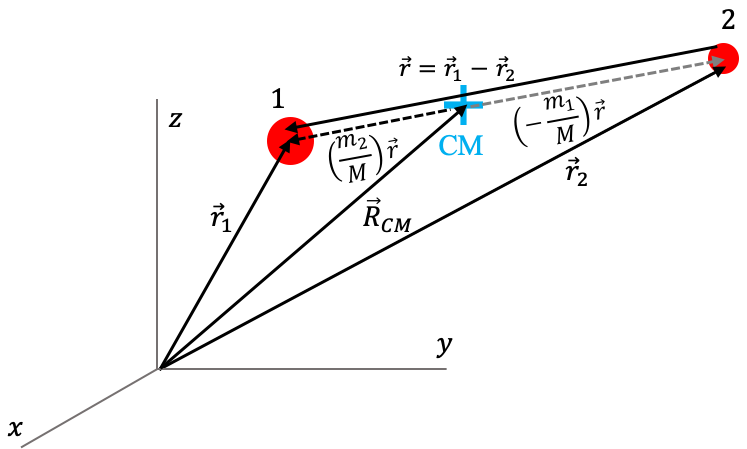
\includegraphics[width=0.8\textwidth]{./figures/horizontal_centro_masa.png}
\caption{Relación entre la posición del centro de masa \(\vec R\), el
vector relativo \(\vec r=\vec{r}_1-\vec{r}_2\) y la posición de las
partículas en un sistema de dos
cuerpos.\label{fig:centro_masa}}
\end{figure}

Como vemos la distancia del centro de masa a cada partícula es
directamente proporcional a la masa de la otra partícula. Así, si
llamamos \(\vec{r}_i'=\vec r_i-\vec R\) al vector que va del centro de
masa a la posición de cada partícula, entonces:

\begin{equation}
\label{eq:distancia_centro_masa}
\frac{r_1'}{r_2'}=\frac{m_2}{m_1}
\end{equation}
\begin{box_history}{Un poco de historia}{}{nofloat}
\small

\textbf{Kepler y el centro de masa.} Muchos años antes de que Newton
hubiera formalizado las leyes de la mecánica, antes de que apareciera el
concepto de masa, fuerza o el postulado de acción y reacción, todos los
cuales son requeridos para la deducción formal de la relación expresada
en la Ec. (\ref{eq:distancia_centro_masa}), Kepler había ya intuido este
resultado. En su obra cumbre \emph{Astronomía Nueva} de 1609, presentó,
entre los que denomino sus \emph{8 axiomas de una teoría verdadera de la
gravedad}, la siguiente afirmación:

\begin{wrapfigure}{l}{0.55\textwidth}
\centering
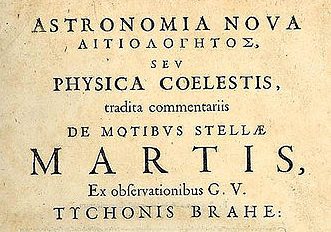
\includegraphics[width=0.5\textwidth]{./figures/vertical_astronomia_nova.png}
\caption{Primera página de la obra cumbre de Kepler \emph{Astronomía
Nova}.\label{fig:astronomia_nova}}
\end{wrapfigure}

\begin{quote}
``\emph{Si la Tierra y la Luna no fueran mantenidas en sus respectivas
órbitas por una fuerza espiritual o de alguna otra naturaleza
equivalente, la Tierra ascendería hacia la Luna 1/54 de la distancia y
la Luna descendería las restantes 53 partes del intervalo y así se
unirían. Pero este cálculo presupone que ambos poseen la misma
densidad}.''\footnote{En realidad el centro de masa del sistema
  Tierra-Luna esta a 1/81 de la distancia entre ambos (la masa de la
  Tierra es 81 veces la de la Luna.) Sin embargo, la estimación de
  Kepler, como bien lo aclara al final de esta cita sin que terminemos
  de entenderle, se basaba en la suposición de que la masa de nuestro
  satélite se puede estimar exclusivamente a partir de su tamaño. Usando
  el valor contemporáneo del radio de la Luna y de la Tierra, la masa
  estimada de nuestro satélite, a partir de su tamaño y suponiendo
  densidades iguales, sería
  \((R_\mathrm{Luna}/R_\mathrm{Tierra})^3=(1737/6371)^3=1/49\) de la
  masa de la Tierra, que es cercano al valor de 1/54 usado por Kepler.}
\end{quote}

Este hecho pone en evidencia dos cosas: (1) la clarividencia del
matemático alemán, quién entre otras cosas además de la citada, intuyó
algunas importantes propiedades de la gravedad y de sus efectos sobre el
movimiento planetario 80 años antes que Newton y sus contemporáneos; y
(2) que las ideas de la mecánica que hoy atribuímos exclusivamente a
Newton estaban ``flotando'' en el ambiente intelectual de su época desde
hacía casi 100 años. Newton, como lo sería también Maxwell un siglo y
medio después en el caso de la electricidad y el magnetismo, fue en
cierto sentido un compilador de la sabiduría ``mecánica'' de su época.

\end{box_history}
\hypertarget{teoremas_conservacion}{%
\subsection{Teoremas de conservación}\label{teoremas_conservacion}}

Usando la e.d.m. para un sistema de partículas (Ec. \ref{}) y algunas de
las deducciones que ya habíamos realizado en el caso de partículas
individuales, podemos deducir algunos teoremas mecánicas de gran
importancia.
\begin{box_theorem}{Proposición}{box:teo:conservacion.p.sistemas}

\textbf{Teorema de conservación del momentum lineal.} Si la fuerza
externa total sobre un sistema de partículas es nula, el momentum total
del sistema se mantiene constante. En términos matemáticos:

\[
  \vec{F}^\mathrm{E}=\sum_i \vec{F}_i^\mathrm{E}=0\Longleftrightarrow \vec{P}=\vec{P}_\mathrm{CM}
  \]

Donde \(\vec{P}_\mathrm{CM}\) es un vector constante.

\end{box_theorem}
Este teorema ocupa un lugar central en la mecánica y sus implicaciones
no son para nada triviales. Piense tan solo en el hecho de que aún si un
sistema contiene un enorme número de partículas, que rebotan entre sí o
se dispersan unas contra otras, procesos en los cuáles el momento de las
partículas se modifica de formas a veces inesperadas, la suma de todos
los momentos individuales producirá siempre el mismo número.

Premultiplicamos ahora la e.d.m. en la Ec. (\ref{eq:edm_sistema}) por el
factor integrante \(\vec{r}_i\times\) y sumando sobre todas las
partículas:

\[
\sum_i m_i r_i\times\ddot{r}_i=\sum_i\vec{r}_i\times\left(\vec{F}^E_i + \sum_{j\neq i}\vec{F}_{ij}\right)
\]

El lado izquierdo izquierdo de esta última ecuación se puede expresar en
términos de cuadraturas (ver \autoref{integracion_edm}), de modo que
la ecuación adopta la forma más conveniente de:

\[
\frac{\mathrm{d}}{\mathrm{d}t}\left(\sum_i m_i r_i\times\dot{r}_i\right)=\vec{r}_i\times\sum\left(\vec{F}^E_i + \vec{F}_{ij}\right),
\] donde reconocemos, del lado izquierdo al momento angular total
\(\vec L=\sum m_i\vec{r}_i\times\dot{\vec{r}}_i\) y del derecho la torca
neta:

\begin{equation}
\label{eq:torca_sistema}
\vec \tau=\vec{r}_i\times\sum\left(\vec{F}^E_i + \vec{F}_{ij}\right).
\end{equation}

En términos de estas cantidades, la e.d.m. de un sistema de particulas
se puede escribir, alternativamente, como:

\begin{equation}
\label{eq:dLdt_sistema_torca}
\dot{\vec{L}}=\tau
\end{equation}

Volvamos a la torca. Por el postulado de acción y reacción (Pos.
\ref{box:pos:accion.reaccion}) las torcas de las fuerzas entre las
partículas se pueden agrupar por pares de la forma:

\[
\vec r_k\times \vec F_{lk}+\vec r_l \times \vec F_{kl}=-\vec{r}_{lk}\times \vec F_{lk},
\] donde \(\vec{r}_{lk}=\vec{r}_l-\vec{r}_k\) es el vector relativo, y
hemos usado índices \(l,k\) distintos a los originales \(i,j\) de la
e.d.m. para evitar confusiones.

Si adicionalmente, las interacciones son tales que el postulado de
acción y reacción fuerte se cumple, es decir si
\(\vec{r}_{lk}\parallel \vec{F}_{lk}\), entonces todas las torcas
internas se cancelan mutuamente y como consecuencia:

\begin{equation}
\label{eq:torque_sistema}
\vec{\tau} = \sum \vec{r}_i\times \vec{F}^E_i,
\end{equation} de donde, finamente, la e.d.m. del sistema de partículas
(Ec. \ref{eq:dLdt_sistema_torca}) tiene la forma explícita:

\[
\dot{\vec{L}}=\sum \vec{r}_i\times \vec{F}^E_i
\]

Esta última ecuación conduce a un segundo importante teorema de
conservación:
\begin{box_theorem}{Proposición}{box:teo:conservacion.L.sistemas}

\textbf{Teorema de conservación del momentum angular.} Si la torca
externa total sobre un sistema de partículas es nula, el momento angular
total del sistema se mantiene constante. En términos matemáticos:

\[
  \vec{\tau} = \sum \vec{r}_i\times \vec{F}^E_i=\vec 0\Longleftrightarrow \vec{L}=\vec{L}_\mathrm{0}
  \]

Donde \(\vec{L}_\mathrm{0}\) es un vector constante.

\end{box_theorem}
Es claro que la condición básica del teorema de conservación del momento
angular (torque neto nulo) se cumple también en el caso en el que las
fuerzas externas son nulas. Es decir, en un sistema aislado de
partículas, tanto el momento lineal como el momento angular se
conservan.

De nuevo, por trivial que nos parezca el teorema de conservación del
momento angular, esta lejos de serlo. La cantidad implicada aquí es
mucho más compleja que el momento lineal y resulta sencillamente
increíble que bajo una condición tan particular como la que supone el
teorema, una combinación no trivial de cantidades cinemáticas produzcan
un vector constante.

Pongamos a prueba el teorema usando el sistema de partículas que
habíamos introducido en la \autoref{fuerzas_centro_masa}. Para ello
calculemos el momento angular total del sistema:

    \begin{code}{Algoritmo}{code:L_sistema_ejemplo}\begin{Verbatim}[fontsize=\small,commandchars=\\\{\}]
\PY{c+c1}{\PYZsh{}Momento angular de cada partícula}
\PY{k+kn}{from} \PY{n+nn}{numpy} \PY{k}{import} \PY{n}{cross}
\PY{n}{Ls}\PY{o}{=}\PY{n}{ms}\PY{p}{[}\PY{p}{:}\PY{p}{,}\PY{k+kc}{None}\PY{p}{]}\PY{o}{*}\PY{n}{cross}\PY{p}{(}\PY{n}{rs}\PY{p}{,}\PY{n}{vs}\PY{p}{)}

\PY{c+c1}{\PYZsh{}Momento angular total}
\PY{n}{L}\PY{o}{=}\PY{n+nb}{sum}\PY{p}{(}\PY{n}{Ls}\PY{p}{)}
\end{Verbatim}

%%

\end{code}
\vspace{-1em}

%%hidecode


    \begin{Verbatim}[fontsize=\small,commandchars=\\\{\}]
Momentos angulares individuales:
[[ 0.    0.    1.35]
 [ 0.   -0.   -6.25]
 [ 0.   -0.   -3.72]]
Momento angular total:
[ 0.    0.   -8.62]
\end{Verbatim}

Propaguemos ahora sus posiciones y velocidades asumiendo que las
partículas se mueven con velocidad constante, es decir, sin experimentan
ninguna fuerza de interacción mutua, y más importante, ninguna fuerza
externa. En esta condición dinámica las velocidades no se modifican:

    \begin{code}{}{}\begin{Verbatim}[fontsize=\small,commandchars=\\\{\}]
\PY{c+c1}{\PYZsh{}Tiempo futuro}
\PY{n}{t}\PY{o}{=}\PY{l+m+mf}{10.0}

\PY{c+c1}{\PYZsh{}Posición y velocidad de las partículas en t}
\PY{n}{rs\PYZus{}t}\PY{o}{=}\PY{n}{rs}\PY{o}{+}\PY{l+m+mi}{10}\PY{o}{*}\PY{n}{vs}
\PY{n}{vs\PYZus{}t}\PY{o}{=}\PY{n}{vs}
\end{Verbatim}

%%

\end{code}
\vspace{-1em}

%%hidecode


    \begin{Verbatim}[fontsize=\small,commandchars=\\\{\}]
Posiciones iniciales: rs =
[[0.33 1.93 0.  ]
 [1.98 0.47 0.  ]
 [0.81 0.27 0.  ]]
Posiciones finales: vs =
[[ 0.4   2.99  0.  ]
 [ 0.34 -0.75  0.  ]
 [-0.25 -0.77  0.  ]]
\end{Verbatim}

Véamos ahora cuánto valen los momentos angulares individuales y total,
después de que las partículas se propagaran:

    \begin{code}{}{}\begin{Verbatim}[fontsize=\small,commandchars=\\\{\}]
\PY{c+c1}{\PYZsh{}Momento angular de cada partícula}
\PY{k+kn}{from} \PY{n+nn}{numpy} \PY{k}{import} \PY{n}{cross}
\PY{n}{Ls\PYZus{}t}\PY{o}{=}\PY{n}{ms}\PY{p}{[}\PY{p}{:}\PY{p}{,}\PY{k+kc}{None}\PY{p}{]}\PY{o}{*}\PY{n}{cross}\PY{p}{(}\PY{n}{rs\PYZus{}t}\PY{p}{,}\PY{n}{vs\PYZus{}t}\PY{p}{)}

\PY{c+c1}{\PYZsh{}Momento angular total}
\PY{n}{L\PYZus{}t}\PY{o}{=}\PY{n}{Ls\PYZus{}t}\PY{o}{.}\PY{n}{sum}\PY{p}{(}\PY{n}{axis}\PY{o}{=}\PY{l+m+mi}{0}\PY{p}{)}
\end{Verbatim}

%%

\end{code}
\vspace{-1em}

%%hidecode


    \begin{Verbatim}[fontsize=\small,commandchars=\\\{\}]
Momentos angulares después:
[[ 0.    0.    1.35]
 [ 0.   -0.   -6.25]
 [ 0.    0.   -3.72]]
Momento angular total después:
[ 0.    0.   -8.62]
\end{Verbatim}

El momento angular total después de la propagación resulta igual al
momento angular antes de ella (Alg. \ref{code:L_sistema_ejemplo}) con lo
que comprobamos que en la ausencia de fuerzas externas, incluso frente a
modificaciones no triviales de las posiciones, el momento angular se
mantiene constante.

\hypertarget{dinamica_centro_masa}{%
\subsection{Dinámica referida al centro de
masa}\label{dinamica_centro_masa}}

Una forma especial de las e.d.m. de un sistema de partículas, se obtiene
cuando lo describimos desde un sistemade referencia ``atado'' del centro
de masa (origen en el centro de masa y velocidad igual a él.)

Usando las transformaciones de Galileo (Pos.
\ref{box:pos:transformaciones.galileo}) la posición y velocidad de cada
partícula referida al centro de masa será (Ecs.
\ref{eq:ley_adicion_velocidades} y \ref{eq:transformaciones_galileo}):

\begin{equation}
\label{eq:estado_CM}
\begin{array}{rcl}
\vec r_i(t) & = & \vec R_\mathrm{CM}(t)+\vec{r}_i'(t)\\
\vec v_i(t) & = & \vec V_\mathrm{CM}(t)+\vec{v}_i'(t) \\
\end{array}
\end{equation}

Aquí, las cantidades primadas están referidas al nuevo sistema de
referencia. En general
\(\vec{R}_\mathrm{CM}(t)=\int \vec{V}_\mathrm{CM}(t)\;\mathrm{d}t\) será
la posición del centro de masa en \(t\).

\hypertarget{momento-angular-total-del-sistema}{%
\subsubsection{Momento angular total del
sistema}\label{momento-angular-total-del-sistema}}

En el sistema de referencia del centro de masa el momentum angular es:

\[
\begin{array}{rcl}
\vec L & = & \sum_i \vec r_i \times \vec p_i \\
       & = & \sum_i m_i(\vec R_\mathrm{CM}+\vec{r}_i')\times (\vec V_\mathrm{CM}+\vec{v}_i')\\
       & = & (\sum_i m_i)\vec R_\mathrm{CM}\times\vec V_\mathrm{CM}+\vec R_\mathrm{CM}\times(\sum_i m_i\vec{v}_i')+
             (\sum_i m_i\vec{r}_i')\times\vec{V_\mathrm{CM}}+
             \sum_i (m_i\vec{r}_i'\times\vec{v}_i')
\end{array}
\]

En esta expresión \(\sum m_i\vec{r}_i'\) y \(\sum m_i\vec{v}_i'\) son,
respectivamente, vectores proporcionales a la posición y velocidad del
centro de masa (ver Ec. \ref{eq:centro_masa}), pero medidos en el
sistema de referencia del mismo centro de masa; por definción, ambas
cantidades son entonces nulas (para una sencilla comprobación numérica,
ver algoritmos abajo.)

Finalmente, el momento angular total del sistema se puede escribir como:

\begin{equation}
\label{eq:L_CM_interno}
\vec L = \vec R_\mathrm{CM}\times \vec P_\mathrm{CM} + \sum_i \vec r'_i\times \vec p'_i
\end{equation} es decir, \textbf{el momento angular total de un sistema
de partículas} es es igual a la suma del \textbf{momento angular del
centro de masa} y el \textbf{momentum angular total de las partículas en
el sistema de referencia del centro de masa}.

Nuevamente podemos comprobar este resultado usando el sistema de ejemplo
que introdujimos en \autoref{fuerzas_centro_masa}.

Calculemos primero el momento angular del centro de masa del sistema:

    \begin{code}{}{}\begin{Verbatim}[fontsize=\small,commandchars=\\\{\}]
\PY{c+c1}{\PYZsh{}Momento angular del centro de masaa}
\PY{k+kn}{from} \PY{n+nn}{numpy} \PY{k}{import} \PY{n}{cross}
\PY{n}{L\PYZus{}CM}\PY{o}{=}\PY{n}{M}\PY{o}{*}\PY{n}{cross}\PY{p}{(}\PY{n}{R\PYZus{}CM}\PY{p}{,}\PY{n}{V\PYZus{}CM}\PY{p}{)}
\end{Verbatim}

%%

\end{code}
\vspace{-1em}

%%hidecode


    \begin{Verbatim}[fontsize=\small,commandchars=\\\{\}]
Momento angular del centro de masa:
[ 0.   -0.    7.96]
\end{Verbatim}

Para calcular el momento angular de las partículas en el sistema de
referencia del centro de masa, debemos primero calcular la posición y
velocidad de ellas en ese sistema usando las Ecs. (\ref{eq:estado_CM}):

    \begin{code}{}{}\begin{Verbatim}[fontsize=\small,commandchars=\\\{\}]
\PY{c+c1}{\PYZsh{}Posición y velocidad referida al centro de masa}
\PY{k+kn}{from} \PY{n+nn}{numpy} \PY{k}{import} \PY{n}{subtract}
\PY{n}{rps}\PY{o}{=}\PY{n}{subtract}\PY{p}{(}\PY{n}{rs}\PY{p}{,}\PY{n}{R\PYZus{}CM}\PY{p}{)}
\PY{n}{vps}\PY{o}{=}\PY{n}{subtract}\PY{p}{(}\PY{n}{vs}\PY{p}{,}\PY{n}{V\PYZus{}CM}\PY{p}{)}
\end{Verbatim}

%%

\end{code}
\vspace{-1em}

%%hidecode


    \begin{Verbatim}[fontsize=\small,commandchars=\\\{\}]
Posiciones respecto al CM:
[[-0.56  0.98]
 [ 1.09 -0.48]
 [-0.08 -0.68]]
Velocidades respecto al CM:
[[ 0.08  0.13]
 [-0.09 -0.09]
 [-0.03 -0.08]]
\end{Verbatim}

Con este resultado podemos verificar la afirmación que habíamos hecho en
la deducción de la Ec. (\ref{eq:L_CM_interno}), en la que habíamos dicho
que \(\sum m_i\vec{r}_i'\) y \(\sum m_i\vec{v}_i'\) son vectores nulos:

    \begin{code}{}{}\begin{Verbatim}[fontsize=\small,commandchars=\\\{\}]
\PY{n}{R\PYZus{}CM\PYZus{}CM}\PY{o}{=}\PY{n+nb}{sum}\PY{p}{(}\PY{n}{ms}\PY{p}{[}\PY{p}{:}\PY{p}{,}\PY{k+kc}{None}\PY{p}{]}\PY{o}{*}\PY{n}{rps}\PY{p}{)}\PY{o}{/}\PY{n}{M}
\PY{n}{V\PYZus{}CM\PYZus{}CM}\PY{o}{=}\PY{n+nb}{sum}\PY{p}{(}\PY{n}{ms}\PY{p}{[}\PY{p}{:}\PY{p}{,}\PY{k+kc}{None}\PY{p}{]}\PY{o}{*}\PY{n}{vps}\PY{p}{)}\PY{o}{/}\PY{n}{M}
\end{Verbatim}

%%

\end{code}
\vspace{-1em}

%%hidecode


    \begin{Verbatim}[fontsize=\small,commandchars=\\\{\}]
Posiciones del CM respecto al CM:
[1.53e-16 0.00e+00]
Posiciones del CM respecto al CM:
[-3.95e-18  5.26e-18]
\end{Verbatim}

Hecha esta verificación, podemos ahora calcular el momento angular total
de las partículas en el sistema de referencia del centro de masa:

    \begin{code}{}{}\begin{Verbatim}[fontsize=\small,commandchars=\\\{\}]
\PY{c+c1}{\PYZsh{}Momento angular de cada partícula}
\PY{k+kn}{from} \PY{n+nn}{numpy} \PY{k}{import} \PY{n}{cross}
\PY{n}{Lps}\PY{o}{=}\PY{n}{ms}\PY{p}{[}\PY{p}{:}\PY{p}{,}\PY{k+kc}{None}\PY{p}{]}\PY{o}{*}\PY{n}{cross}\PY{p}{(}\PY{n}{rps}\PY{p}{,}\PY{n}{vps}\PY{p}{)}

\PY{c+c1}{\PYZsh{}Momento angular total}
\PY{n}{Lp}\PY{o}{=}\PY{n+nb}{sum}\PY{p}{(}\PY{n}{Lps}\PY{p}{)}
\end{Verbatim}

%%

\end{code}
\vspace{-1em}

%%hidecode


    \begin{Verbatim}[fontsize=\small,commandchars=\\\{\}]
Momento angular total referido al centro de masa:
[  0.     0.   -16.58]
\end{Verbatim}

Ciertamente este vector no coincide con el momentum angular total
referido al origen que habíamos calculado en el Alg.
(\ref{code:L_sistema_ejemplo}); pero esto es natural puesto que no hemos
sumado el momento angular del centro de masa que calculamos antes:

    \begin{code}{}{}\begin{Verbatim}[fontsize=\small,commandchars=\\\{\}]
\PY{c+c1}{\PYZsh{}Momento angular total}
\PY{n}{L}\PY{o}{=}\PY{n}{L\PYZus{}CM}\PY{o}{+}\PY{n}{Lp}
\end{Verbatim}

%%

\end{code}
\vspace{-1em}

%%hidecode


    \begin{Verbatim}[fontsize=\small,commandchars=\\\{\}]
Momento angular total:
[ 0.    0.   -8.62]
\end{Verbatim}

Que coincide con el obtenida con el Alg. (\ref{code:L_sistema_ejemplo}).
Con esto hemos comprobado la relación expresada en la Ec.
(\ref{eq:L_CM_interno}).

\hypertarget{energuxeda-cinuxe9tica-total-del-sistema}{%
\subsubsection{Energía cinética total del
sistema}\label{energuxeda-cinuxe9tica-total-del-sistema}}

Una relación similar a la encontrada en la Ec. (\ref{eq:L_CM_interno})
para el momento angular, puede deducirse también para el caso de la
energía cinética total \(K\).

Usando el teorema del trabajo y energía (Teo.
\ref{box:teo:trabajo.energia}) puede probarse que en el caso de un
sistema de partículas \(K\) es:

\[
K=\frac{1}{2}\sum m_i v_i^2
\]

Reemplazando en esta expresión la velocidad de cada partícula en el
sistema original por su velocidad en el sistema de referencia del centro
de masa, \(\vec{v}_i=\vec{v}_i'+\vec{V}\) (Ec. \ref{eq:estado_CM}) se
obtiene:

\[
K=
\frac{1}{2}\sum m_i \vec V^2+
\vec V\cdot\frac{\mathrm{d}}{\mathrm{d}t}\left(\sum m_i \vec{r}_i'\right)+
\frac{1}{2}\sum m_i\vec{v}_i'^2
\] de donde por los mismos argumentos en la deducción de la Ec.
(\ref{eq:L_CM_interno}) obtenemos finalmente:

\begin{equation}
\label{eq:K_CM_interno}
K = \frac{1}{2} M V^2 + \frac{1}{2} \sum m_i {v_i}'^2,
\end{equation} es decir la \textbf{energía cinética total del sistema}
es igual a \textbf{la energía cinética del centro de masa} más
\textbf{la energía cinética total referida al centro de masa} (energía
interna.)

De nuevo podemos verificar este resultado usando el sistema de ejemplo.

Para ello, primero calculemos la energía cinética total usando las
velocidades referidas al sistema de referencia original:

    \begin{code}{Algoritmo}{code:K_sistema_ejemplo}\begin{Verbatim}[fontsize=\small,commandchars=\\\{\}]
\PY{c+c1}{\PYZsh{}Magnitud de las velocidades de las partículas}
\PY{k+kn}{from} \PY{n+nn}{numpy}\PY{n+nn}{.}\PY{n+nn}{linalg} \PY{k}{import} \PY{n}{norm}
\PY{n}{vmags}\PY{o}{=}\PY{n}{norm}\PY{p}{(}\PY{n}{vs}\PY{p}{,}\PY{n}{axis}\PY{o}{=}\PY{l+m+mi}{1}\PY{p}{)}

\PY{c+c1}{\PYZsh{}Energía cinética individual de cada partícula}
\PY{n}{Ks}\PY{o}{=}\PY{l+m+mf}{0.5}\PY{o}{*}\PY{n}{ms}\PY{o}{*}\PY{n}{vmags}\PY{o}{*}\PY{o}{*}\PY{l+m+mi}{2}

\PY{c+c1}{\PYZsh{}Energía cinética total}
\PY{n}{K}\PY{o}{=}\PY{n+nb}{sum}\PY{p}{(}\PY{n}{Ks}\PY{p}{)}
\end{Verbatim}

%%

\end{code}
\vspace{-1em}

%%hidecode


    \begin{Verbatim}[fontsize=\small,commandchars=\\\{\}]
Energía cinética de las partículas:
[0.37 0.79 0.73]
Energía cinética total: 1.90
\end{Verbatim}

Ahora podemos hacerlo usando la nueva expresión:

    \begin{code}{}{}\begin{Verbatim}[fontsize=\small,commandchars=\\\{\}]
\PY{c+c1}{\PYZsh{}Energía cinética del centro de masa:}
\PY{n}{K\PYZus{}CM}\PY{o}{=}\PY{l+m+mf}{0.5}\PY{o}{*}\PY{n}{M}\PY{o}{*}\PY{n}{norm}\PY{p}{(}\PY{n}{V\PYZus{}CM}\PY{p}{)}\PY{o}{*}\PY{o}{*}\PY{l+m+mi}{2}

\PY{c+c1}{\PYZsh{}Magnitud de las velocidades}
\PY{n}{vpmags}\PY{o}{=}\PY{n}{norm}\PY{p}{(}\PY{n}{vps}\PY{p}{,}\PY{n}{axis}\PY{o}{=}\PY{l+m+mi}{1}\PY{p}{)}

\PY{c+c1}{\PYZsh{}Energía cinética individual de cada partícula}
\PY{n}{Kps}\PY{o}{=}\PY{l+m+mf}{0.5}\PY{o}{*}\PY{n}{ms}\PY{o}{*}\PY{n}{vpmags}\PY{o}{*}\PY{o}{*}\PY{l+m+mi}{2}

\PY{c+c1}{\PYZsh{}Energía cinética en el centro de masa}
\PY{n}{Kp}\PY{o}{=}\PY{n}{Kps}\PY{o}{.}\PY{n}{sum}\PY{p}{(}\PY{p}{)}

\PY{c+c1}{\PYZsh{}Energía total}
\PY{n}{K}\PY{o}{=}\PY{n}{K\PYZus{}CM}\PY{o}{+}\PY{n}{Kp}
\end{Verbatim}

%%

\end{code}
\vspace{-1em}

%%hidecode


    \begin{Verbatim}[fontsize=\small,commandchars=\\\{\}]
Energía cinética del CM: 0.5505136059795793
Energía cinética de las partículas (respecto al CM): [0.8  0.32 0.22]
Energía cinética total (respecto al CM): 1.35
Energía cinética total: 1.90
\end{Verbatim}

De nuevo, la energía cinética calculada con la Ec.
(\ref{eq:K_CM_interno}) coincide con la obtenida en el Alg.
(\ref{code:K_sistema_ejemplo}).



\hypertarget{sistemas_no_inerciales}{%
\section{Dinámica en sistemas de referencia no
inerciales}\label{sistemas_no_inerciales}}

Todas los postulados y teoremas que describen la dinámica de partículas
y sistemas de partículas introducidos en las secciones anteriores,
tienen validez, como se expreso desde el principio, en sistemas de
referencia inerciales (ver Def. \ref{box:def:sistemas.inerciales}).

¿Cómo se modifican (si se modifican) esos postulaods y teoremas si por
necesidad o ``construcción'' es necesario describir la dinámica de una
partícula o un sistema de partículas respecto de un sistema de
referencia no inercial?

Suponga por ejemplo que queremos describir la dinámica del vuelo de un
cohete respecto a la superficie de la Tierra. Si bien es posible
pasarnos al sistema de referencia del centro del planeta (que es
aproximadamente inercial), por razones prácticas es preferible, al menos
al principio del movimiento, describir las cantidades cinemáticas y
dinámicas del cohete respecto a la plataforma de lanzamiento o bien a la
superficie alrededor de ella. Un sistema de referencia fijado así, ya no
puede considerarse un sistema de referencia inercial (debido a la
rotación de la Tierra).

Suponga ahora que un astronauta quiere hacer un experimento mecánico en
el interior de la estación espacial internacional. Naturalmente allí,
será mejor referir las cantidades cinemáticas y dinámicas a la
estructura de la estación y no al centro de la tierra. De nuevo, para
hacerlo deberá trabajar en un sistema de referencia no inercial.

Estos dos ejemplos sencillos muestran que si bien es más común (y mucho
más conveniente en general) aplicar los postulados y teoremas de la
mecánica en sistemas de referencia inerciales (donde han sido
desarrollados y demostrados) habrán situaciones en las que se hace
obligatorio hacerlo en sistemas de referencia no inerciales.

\hypertarget{transformacion_sistemas_referencia}{%
\subsection{Transformación entre sistemas de
referencia}\label{transformacion_sistemas_referencia}}

En la \autoref{sistemas_referencia} habíamos introducido las
denominadas \emph{transformaciones de Galileo} que son el conjunto de
reglas matemáticas necesarias para convertir las cantidades cinemáticas
o dinámicas \(t\), \(\vec r\), \(\vec v\), \(\vec a\), etc. medidas en
un sistema de referencia inercial \(R\), en el valor de las mismas
cantidades en otro sistema de referencia inercial \(R'\) (ver Definición
\ref{box:pos:transformaciones.galileo}).

Las reglas que postulamos allí eran bastante sencillas:

\begin{equation}
\label{eq:transformaciones_galileo}
\begin{array}{rcl}
t & = & t'\\
\vec r & = & \vec{r}' + \vec u t
\end{array}
\end{equation}

Para extender estas reglas al dominio de la dinámica, podemos agregar el
postulado de que la masa de las partículas es también independiente del
sistema de referencia en el que se la mida:

\begin{equation}
m = m'
\end{equation}

Este postulado se basa en la idea Newtoniana de que la masa es, entre
otras, una medida de la cantidad de materia contenida en un cuerpo, que
no debería depender del observador que la juzgue.

Todos los postulados y teoremas de la dinámica que formulamos en este
capítulo son válidos unicamente si se expresan en las cantidades
cinemáticas y dinámicas que satisfacen estas transformaciones y aquellas
que se derivadan de ellas (como la regla de adición de velocidades y
aceleraciones de las Ecs. \ref{eq:ley_adicion_velocidades} y
\ref{eq:ley_adicion_aceleraciones}).

¿Qué pasa ahora si admitimos la posibilidad de que el sistema \(R'\) se
mueva respecto a \(R\) (que seguiremos asumiendo incercial) con una
velocidad \(u(t)\) que no es constante (el sistema no es inercial)?

Una generalización trivial de las transformaciones de Galileo es (ver
\autoref{fig:transformaciones_noinercial}):

\begin{equation}
\label{eq:transformaciones_acelerado}
\begin{array}{rcl}
t & = & t'\\
\vec r & = & \vec{r}' + \int_0^t \vec u(t)\;\mathrm{d}t\\
m & = & m'\\
\end{array}
\end{equation} en la que hemos asumido que la dirección de los ejes
coordenados de los sistemas se mantiene paralela a lo largo del tiempo.

\begin{figure}[t]
\centering
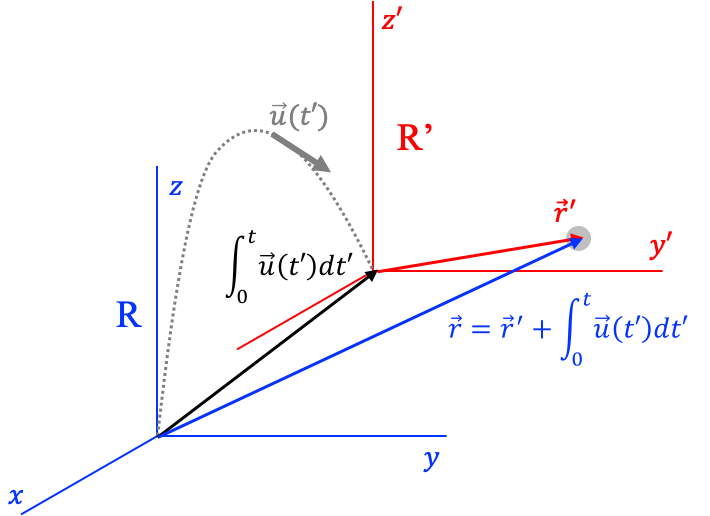
\includegraphics[width=0.7\textwidth]{./figures/square_transformaciones_noinercial.png}
\caption{Construcción geométrica para deducir la regla de transformación
de la posición \(\vec r\) de una partícula (circulo gris) entre un
sistema de referencia inercial \(R\) y uno no inercial \(R'\). Por
construcción los orígenes de ambos sistemas coinciden en t=0. El origen
de coordenadas de \(R'\) se mueve a lo largo de la trayectoria punteada
con velocidad variable
\(\vec u(t')\).\label{fig:transformaciones_noinercial}}
\end{figure}

Usando estas transofrmaciones básicas, es posible deducir las reglas de
transformación para otras cantidades cinemáticas y dinámicas. Así por
ejemplo:

\begin{eqnarray}
\label{eq:v_no_inercial}
\vec{v}' & = & \vec{v}-\vec u(t)\\
\label{eq:p_no_inercial}
\vec{p}' & = & \vec{p}-m\vec u(t)\\
\label{eq:a_no_inercial}
\vec{a}' & = & \vec{a}-\dot{\vec u}\\
\label{eq:F_no_inercial}
\vec{\cal F}' & = & \vec{\cal F}-m\dot{\vec u}
\end{eqnarray}

Estas transformaciones nos permiten comprobar cómo se modifica la
validez de los postulados de la dinámica y de los teoremas defivados de
ellos, al pasar a un sistema de referencia no inercial.

Considere por ejemplo el caso de una partícula que se mueve libre de
fuerzas aplicadas, y por tanto que tiene, en el sistema de referencia
inercial \(R\), velocidad \(\vec v\) (o momentum lineal \(\vec p\))
constantes (obedenciendo el teorema de inercia). Según la regla de
transformación en la Ec. (\ref{eq:v_no_inercial}), la velocidad
\(\vec{v}'\) de la partícula en el sistema no inercial \(R'\) (y por lo
tanto su momentum lineal \(\vec{p}'\)) ya no serán constantes: su valor
dependerá de la velocidad instantánea del sistema \(R'\) respecto de
\(R\), \(u(t)\), que a su vez cambia en el tiempo. \textbf{El teorema de
inercia ya no es válido en \(R'\)}. Es justamente por esto que decimos
que \(R'\) es un sistema de referencia \textbf{no inercial}.

Un caso partícular de esta última situación, pone de relieve los
aparentemente extraños comportamientos que podríamos percibir en
sistemas de referencia no inerciales. La misma partícula del párrafo
anterior, dejada en reposo en \(R\) en \(t\) (y que se mantendría en
reposo respecto a \(R\) en virtud del teorema de inercia), empezará a
moverse con velocidad \(-\vec u(0)\) respecto a \(R'\) sin que se
aplique sobre ella ninguna fuerza.

Este tipo de comportamientos es el que explica, por ejemplo, porque una
persona que no se sostiene de las barandas del Metro en el momento en el
que inicia su marcha, empezará a desplazarse, sin que nada o nadie actúe
sobre ella en el interior del vagón.

Así mismo, incluso en la presencia de fuerzas aplicadas, el postulado de
fuerzas no será válido en el sistema de referencia \(R'\). Según este
postulado, en el sistema de referencia inercial (\(R\)) la fuerza
resultante sobre una partícula es iguales a la fuerza aplicada neta:

\[
\vec{\cal F} = \vec F
\]

o lo que es lo mismo:

\[
\vec{a} = \frac{\vec F}{m}
\]

De acuerdo a la Ec. (\ref{eq:F_no_inercial}) en el sistema de referencia
no inercial:

\begin{equation}
\label{eq:F_aplicada_no_inercial}
\vec{\cal F}' = \vec F - m\dot{\vec u}
\end{equation}

o bien

\[
\vec{a}' = \frac{\vec F}{m} - \dot{\vec u}
\]

Es decir, las fuerzas resultantes en el sistemas de referencia no
inercial, serán iguales a las fuerzas aplicadas \emph{más} una fuerza
resultante \(-m\dot{\vec u}\) que apunta en dirección contraria a la
aceleración relativa entre los sistemas de referencia. Dado que esta
fuerza resultante \emph{nueva} no es producto de la acción de una fuerza
aplicada, la llamamos convencionalmente una \emph{fuerza ficticia}.

En el interior de la estación espacial internacional, por ejemplo, los
cuerpos que flotan en el aire experimentan solo una fuerza aplicada:
aquella debida a la interacción gravitacional con la Tierra (asumimos
que la fuerza gravitacional de los astronautas y la estación es
completamente despreciable). Esta fuerza no es despreciable y es igual a
su peso medido a la altura de la estación (ver
\autoref{fig:iss_microgravedad})\footnote{La estación espacial
  internacional se encuentra a apenas 400 km de altura sobre la
  superficie de la Tierra. Por lo tanto el peso de los cuerpos que
  transporta es apenas \(6371^2/(6371+400)^2\approx 0.88\) veces el que
  experimentan en la superficie de la Tierra (6371 km es el radio
  promedio de la Tierra).}.

\begin{figure}[t]
\centering
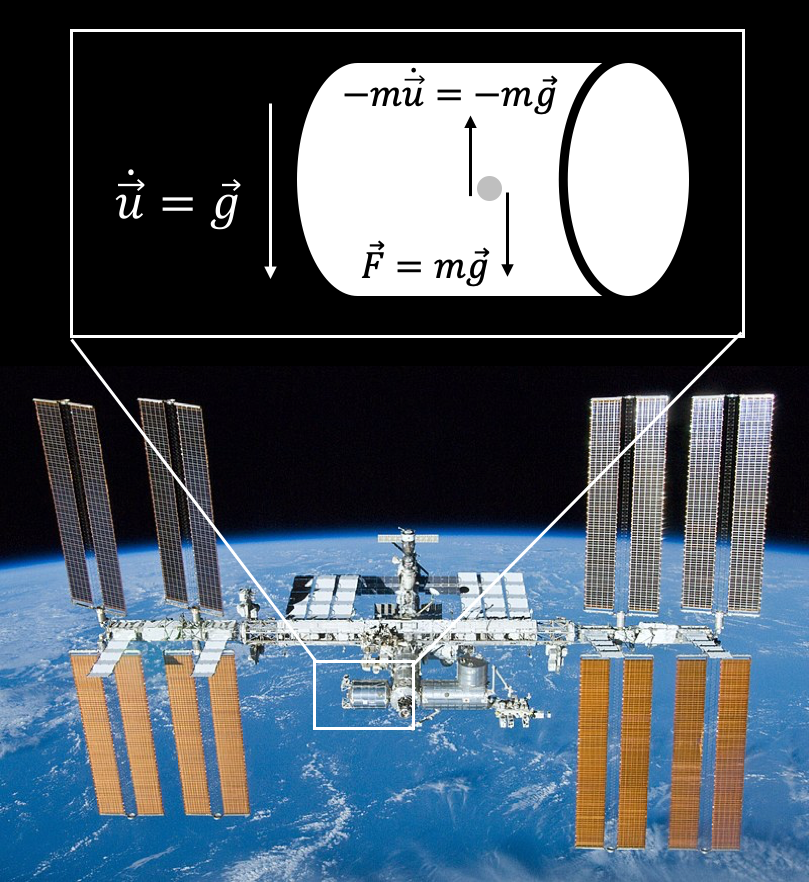
\includegraphics[width=0.5\textwidth]{./figures/vertical_iss_microgravedad.png}
\caption{Explicación de la experiencia de ingravidez en el interior de
un vehículo espacial, en este caso un módulo de la Estación Espacial
Internacional. El módulo corresponde a un sistema de referencia no
inercial con una aceleración \(\dot{\vec{u}}\) igual a la aceleración de
la gravedad \(\vec g\) a la altura de la estación. Una partícula
(círuclo gris) experimenta una fuerza aplicada \(\vec F=m\vec g\) igual
a su peso a la altura de la estación. Sin embargo, por encontrarse en un
sistema de referencia no inercial a esa fuerza debe sumarse la fuerza
ficticia \(-m\dot{\vec{u}}\) que es en magnitud idéntica al peso.
Crédito: NASA/Tripulación de la misión
STS-132.\label{fig:iss_microgravedad}}
\end{figure}

Ahora bien, la fuerza resultante sobre los mismos cuerpos, medida en el
sistema de referencia de la estación, será igual, en virtud de la Ec.
\ref{eq:F_aplicada_no_inercial}, a su peso (la fuerza aplicada) más una
fuerza ficticia que apunta en dirección contraria al centro de la Tierra
(que es hacia donde apunta la aceleración de la estación
\(\dot{\vec{u}}\)) y que es en magnitud proporcional a esa misma
aceleración. Dado que la aceleración de la estación es justamente la
aceleración de la gravedad a esa altura, la fuerza aplicada sobre los
cuerpos y la fuerza ficticia tendrán la misma magnitud.

Como resultado, en el sistema de referencia de la estación los cuerpos
no experimentaran ninguna fuerza resultante y si se colocan en reposo,
permaneceran así, incluso si nada los sostiene. Esta es justamente la
razón de la ilusión de ingravidez que se percibe dentro de la estación y
otros vehículos espaciales que orbitan nuestro planeta.

\hypertarget{sistemas_rotantes}{%
\subsection{Sistemas de referencia rotantes}\label{sistemas_rotantes}}

En los sistemas de referencia acelerados descritos en el apartado
anterior la dirección de los ejes coordenados no cambia en el tiempo con
respecto al sistema de referencia inercial. La rotación de los ejes, es
una segunda forma de producir un sistema de referencia no inercial.

Si suponemos, por simplicidad, que el origen de los sistemas \(R\) y
\(R'\) coinciden durante todo el tiempo, pero los ejes de coordenadas
\(\hat{e}_x'\), \(\hat{e}_y'\), \(\hat{e}_z'\) rotan respecto a un eje
arbitrario, la regla de transformación entre las variables cinemáticas y
dinámicas básicas será:

\begin{eqnarray}
\nonumber
t' & = & t \\
\nonumber
\vec r' & = & \vec r\\
\nonumber
m' & = & m
\end{eqnarray}

En particular, si bien los vectores \(\vec r\) y \(\vec r'\) serán
\emph{geométricamente} idénticos, sus componentes no lo serán:

\[
x {\hat e_x} + y {\hat e_y} + z {\hat e_z} = x' {\hat e_x}' + y' {\hat e_y}' + z' {\hat e_z}'
\]

Esta condición no es única para el vector posición \(\vec r\) sino que
aplica para cualquier cantidad vectorial \(\vec A\) que definamos en el
sistema:

\begin{equation}
\label{eq:A_noinercial}
A_x {\hat e_x} + A_y {\hat e_y} + A_z {\hat e_z} = A_{x'} {\hat e_x}' + A_{y'} {\hat e_y}' + A_{z'} {\hat e_z}'
\end{equation}

Nótese que no hemos escrito \(A_x'\) (dando a entender que el vector
\(\vec A\) cambia al cambiar de sistema de coordenadas) sino \(A_{x'}\)
para indicar que son sus componentes las que cambian.

¿Cómo se relacionan las razones de cambio de
\((\mathrm{d}\vec A/\mathrm{d}t)\) y \((\mathrm{d}\vec A/\mathrm{d}t)'\)
medidas en ambos sistemas de referencia?

Si derivamamos ambos lados de la Ec. (\ref{eq:A_noinercial}) obtenemos:

\begin{eqnarray}
\label{eq:derivada_vector_rotacion_explicita}
\frac{\mathrm{d}A_x}{\mathrm{d}t} {\hat e_x} + \frac{\mathrm{d}A_y}{\mathrm{d}t} {\hat e_y} + \frac{\mathrm{d}A_z}{\mathrm{d}t} {\hat e_z} & = & \frac{\mathrm{d}A_{x'}}{\mathrm{d}t} {\hat e_x}' + \frac{\mathrm{d}A_{y'}}{\mathrm{d}t} {\hat e_y}' + \frac{\mathrm{d}A_{z'}}{\mathrm{d}t} {\hat e_z}' +\\
\nonumber
 & & + A_{x'} \frac{\mathrm{d}{\hat e_x}'}{\mathrm{d}t} + A_{y'} \frac{\mathrm{d}{\hat e_y}'}{\mathrm{d}t} + A_{z'} \frac{\mathrm{d}{\hat e_z}'}{\mathrm{d}t}
\end{eqnarray}

Los vectores unitarios coordenados en el sistema rotante varían
dependiendo del valor instantáneo de la velocidad angular así
\(\omega(t)\) (ver \autoref{fig:rotacion_ejes}):

\begin{eqnarray}
\mathrm{d}\hat{e_x}' & = & \vec{\omega}\times \hat{e_x}' \mathrm{d}t\\
\mathrm{d}\hat{e_y}' & = & \vec{\omega}\times \hat{e_y}' \mathrm{d}t\\
\mathrm{d}\hat{e_z}' & = & \vec{\omega}\times \hat{e_z}' \mathrm{d}t\\
\end{eqnarray} donde \(\vec \omega \equiv \omega \hat n\).

\begin{figure}[t]
\centering
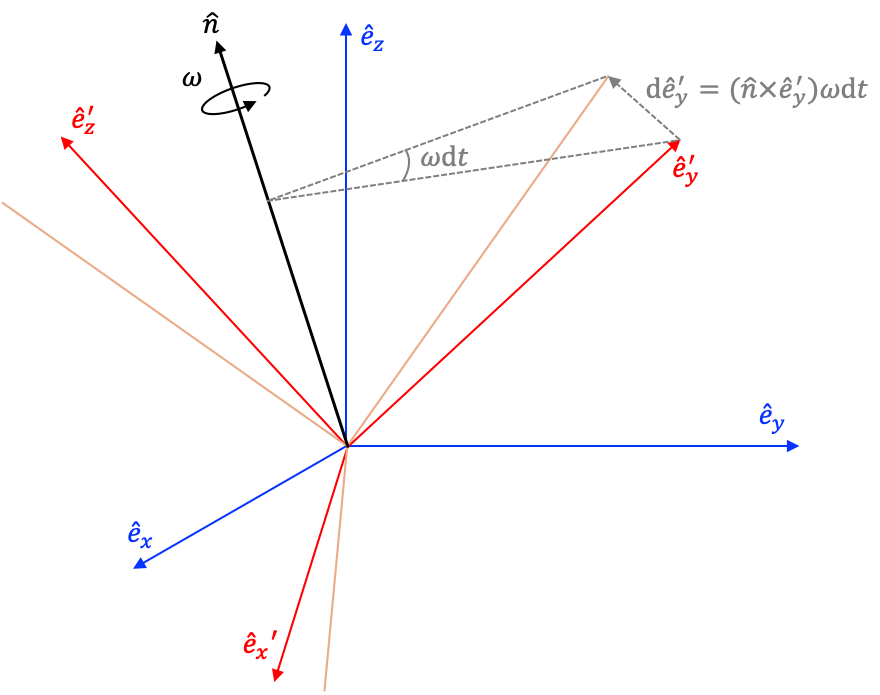
\includegraphics[width=0.7\textwidth]{./figures/square_rotacion_ejes.png}
\caption{Construcción geométrica usada para calcular el cambio en la
dirección de los vectores unitarios coordenados de un sistema de
coordenadas cuando se produce una rotación alrededor de un eje
arbitrario \(\hat n\).\label{fig:rotacion_ejes}}
\end{figure}
\begin{box_note}{Nota}

\textbf{No hay vectores de rotación.} A pesar de que en lo que sigue
usaremos la notación \(\vec\omega\) para referirnos a la cantidad
\(\omega\hat n\), es importante resaltar el hecho que no existe en
matemáticas nada que podamos llamar un \emph{vector de rotación}.

Como señalamos en la \autoref{conjuntos_tuplas_vectores} los
vectores geométricos forman un \emph{espacio vectorial}, sobre cuyos
elementos esta definida una operación interna (la suma vectorial en este
caso) que cumple una serie de condiciones matemáticas, entre ellas la
conmutatividad: el orden en el que se realice una suma de vectores no
debería alterar el resultado de la misma.

Si definimos dos rotaciones que se producen con tasas \(\omega_1\) y
\(\omega_2\) alrededor de ejes diferentes \(\hat n_1\) y \(\hat n_2\) y
queremos determinar el efecto que tienen en un tiempo \(t\) las dos
rotaciones sobre un vector dado (por ejemplo uno de los vectores
unitarios en la \autoref{fig:rotacion_ejes}) no es posible:

\begin{enumerate}
\def\labelenumi{\arabic{enumi}.}
\item
  Definir un ``vector de rotación'' \(\vec\Omega=\Omega\hat N\) que
  represente la operación resultante. Es decir
  \(\vec\Omega\neq \vec\omega_1+\vec\omega_2\).
\item
  Incluso en el caso en el que, de forma ingeniosa o para un caso muy
  particular, pudiéramos definir dicha suma, la conmutatividad no podría
  asegurarse de forma general: las rotaciones no son conmutativas (ver
  \autoref{fig:rotaciones_no_conmutativas}).
\end{enumerate}

\end{box_note}
\begin{figure}[t]
\centering
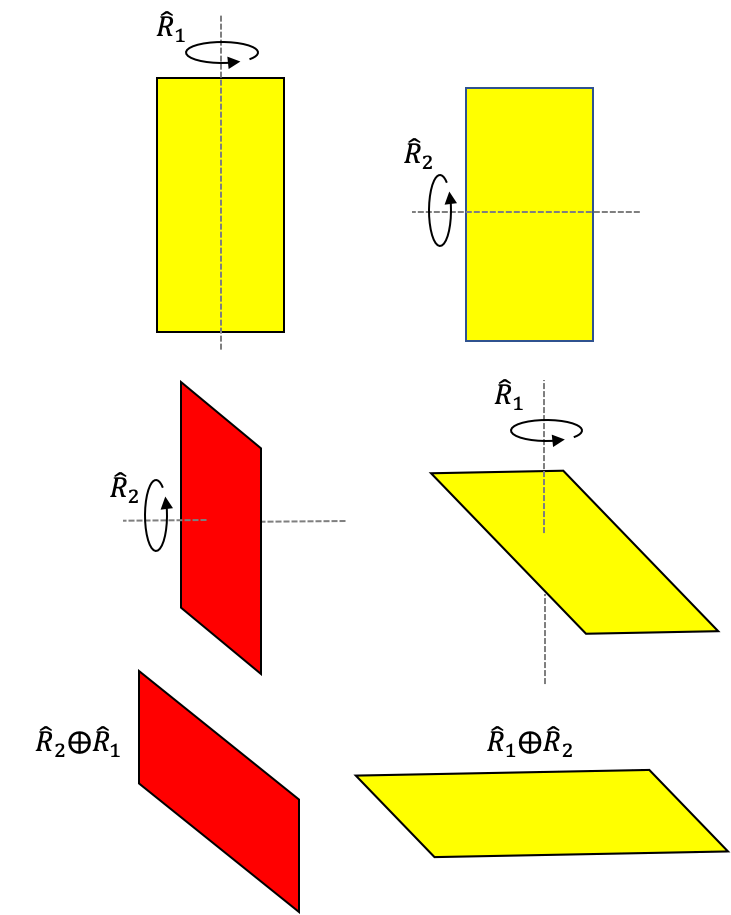
\includegraphics[width=0.7\textwidth]{./figures/vertical_rotaciones_no_conmutativas.png}
\caption{Las rotaciones, representadas aquí por \(\hat R\) no son
operaciones conmutativas. En la columna izquierda se muestra la
aplicación consecutiva (``suma'') de las rotaciones \(\hat R_1\) y
\(\hat R_2\), que hemos representado de forma general como
\(\hat R_2\oplus\hat R_1\). En la columna de la derecha se muestra la
sucesión contraria de operaciones \(\hat R_1\oplus\hat R_2\) que da un
resultado completamente distinto. Es por esta misma razón que en
estricto no es posible definir una suma entre velocidades ángulares y
por lo tanto vectores de velocidad angular. La notación \(\vec\omega\)
es una licencia del lenguaje matemático usaod
aquí.\label{fig:rotaciones_no_conmutativas}}
\end{figure}

Con esto la tasa de cambio descrita por la Ec.
(\ref{eq:derivada_vector_rotacion_explicita}) se puede escribir de la
forma:

\begin{equation}
\label{eq:derivada_vector_rotacion}
\frac{\mathrm{d}}{\mathrm{d}t}\vec A = \frac{\mathrm{d}'}{\mathrm{d}t}\vec A+\vec\omega\times \vec A
\end{equation} donde por los \emph{operadores diferenciales}
\(\mathrm{d}/\mathrm{d}t\) o \(\mathrm{d}'/\mathrm{d}t\) entenderemos
aquí, aquellos que solo actúan sobre las componentes en el sistema de
referencia correspondiente, pero no sobre la dirección de los ejes. Así:

\[
\frac{\mathrm{d}'}{\mathrm{d}t}\vec A \equiv
\frac{\mathrm{d}A_{x'}}{\mathrm{d}t} {\hat e_x}' + \frac{\mathrm{d}A_{y'}}{\mathrm{d}t} {\hat e_y}' + \frac{\mathrm{d}A_{z'}}{\mathrm{d}t} {\hat e_z}'
\]

Por otro lado también es importante aclarar que las cantidades en el
lado derecho de la Ec. (\ref{eq:derivada_vector_rotacion}) deben
escribirse en el sistema de coordenadas rotante, es decir:

\begin{equation}
\label{eq:omega_times_A}
\vec\omega\times \vec A = \vec\omega\times(A_{x'} {\hat e_x}' + A_{y'} {\hat e_y}' + A_{z'} {\hat e_z}')
\end{equation}

Dado que la Ec. (\ref{eq:derivada_vector_rotacion}) es válidad para
cualquier vector libre, podemos definir una regla de transformación
general para la derivada con respecto al tiempo de vectores,
introduciendo el operador diferencial:

\begin{eqnarray}
\frac{d}{dt} =  \frac{d'}{dt}+\vec\omega\;\times
\end{eqnarray} donde se entiende que la cantidad derivada es una
cantidad vectorial.

\hypertarget{adicion_velocidades_rotantes}{%
\subsection{Adición de velocidades en sistemas
rotantes}\label{adicion_velocidades_rotantes}}

Usando estos resultados generales podemos encontrar ahora las reglas de
transformación para la velocidad y la aceleración (los análogos a las
Ecs. \ref{eq:v_no_inercial} y \ref{eq:a_no_inercial}).

En el caso de la velocidad:

\[
\vec v \equiv \frac{\mathrm{d}}{\mathrm{d}t}\vec r = \frac{\mathrm{d'}}{\mathrm{d}t}\vec r + \vec\omega\times\vec r
\]

Por definición, sin embargo:

\[
\vec v'\equiv \frac{\mathrm{d'}\vec r}{\mathrm{d}t}
\] es decir, esta cantidad corresponde a la velocidad de la partícula
medida en el sistema rotante.

De otro lado \(\omega\times\vec r\) debe ser obligatoriamente escrito en
términos de los vectores unitarios coordenados del sistema \(R'\) (ver
Ec. \ref{eq:omega_times_A}):

\[
\omega\times\vec r=\omega\times(x'\hat e_x'+y'\hat e_y'+z'\hat e_z')=\omega\times\vec r'
\]

Con estas definiciones, la ley de ``adición'' de velocidades para un
sistema de referencia rotante se escribe finalmente como:

\begin{equation}
\label{eq:adicion_velocidades_rotante}
\vec v = \vec v' + \vec\omega\times\vec r'
\end{equation}
\begin{box_note}{Nota}

\textbf{Vectores y componentes.} Es muy importante entender que la
Ecuación (\ref{eq:adicion_velocidades_rotante}) representa una relación
entre vectores, no entre sus componentes. Es decir, esta relación
implica por ejemplo que las magnitudes \(|\vec v|\) y
\(|\vec v' + \vec\omega\times\vec r'|\) son iguales, puesto que se trata
de una propiedad vectorial. Sin embargo, las componente \(x\) en ambos
sistemas de referencia no pueden compararse:

\[
v_x \neq v_{x'}+(\vec\omega\times\vec r')_{x'}
\]

Las componentes de los vectores a ambos lados de la Ec.
(\ref{eq:adicion_velocidades_rotante}) se relacionan a través de una
matriz de rotación como se explico en la
\autoref{conicas_rotacion_plano}. En la
\autoref{ejemplo_numerico_rotante} de este mismo capítulo
ilustraremos este importante punto.

\end{box_note}
\hypertarget{aceleraciones_ficticias_rotantes}{%
\subsection{Aceleraciones ficticias en sistemas
rotantes}\label{aceleraciones_ficticias_rotantes}}

Para encontrar la relación entre las acleraciones, basta aplicar un
procedimiento similar al anterior:

\[
\vec a \equiv \frac{\mathrm{d}}{\mathrm{d}t}\vec v = \frac{\mathrm{d'}}{\mathrm{d}t}\vec v + \vec\omega\times\vec v
\] sin embargo las componentes del vector \(\vec v\) en el sistema de
ejes de \(R'\), que son las que deben usarse en el lado derecho de la
ecuación anterior, ya no obedecen reglas tan simples como las de
cualquier otro vector libre, tal como el vector \(\vec r\).

Estas componentes obedecen la regla más compleja expresada por la Ec.
(\ref{eq:adicion_velocidades_rotante}). Reemplazando las componentes de
la velocidad medidas en el sistema inercial, las aceleraciones se
relacionan como:

\[
\vec a = \frac{\mathrm{d'}}{\mathrm{d}t}(\vec v' + \vec\omega\times\vec r') + \vec\omega\times(\vec v' + \vec\omega\times\vec r')
\]

Derivando y reuniendo términos semejantes obtenemos:

\[
\vec a = \vec a'+\vec\omega\times(\vec\omega\times \vec r')+2 \vec \omega\times\vec v'+ \dot{\vec{\omega}}\times \vec r'
\] donde

\[
\vec a'\equiv\frac{\mathrm{d'}}{\mathrm{d}t}\vec v'=\frac{\mathrm{d}v_{x'}}{\mathrm{d}t} {\hat e_x}' + \frac{\mathrm{d}v_{y'}}{\mathrm{d}t} {\hat e_y}' + \frac{\mathrm{d}v_{z'}}{\mathrm{d}t} {\hat e_z}'
\] es la aceleración instantánea que experimenta la partícula medida en
el sistema rotante.

Si despejamos \(\vec a'\) (a la manera como lo hicimos para deducir la
Ec. \ref{eq:a_no_inercial}), obtenemos:

\begin{equation}
\label{eq:ley_adicion_aceleraciones}
\vec a' = \vec a-\vec\omega\times(\vec\omega\times \vec r')-2 \vec \omega\times\vec v'-\dot{\vec{\omega}}\times \vec r'
\end{equation}

A diferencia de lo que observamos en sistemas no inerciales de ejes
fijos, donde en la dinámica emerge una sola aceleración ficticia que es
antiparalela a la aceleración del sistema de referencia
(\(-\dot{\vec{u}}\)), en sistemas rotantes hay tres diferentes
aceleraciones ficticias:

\begin{figure}[t]
\centering
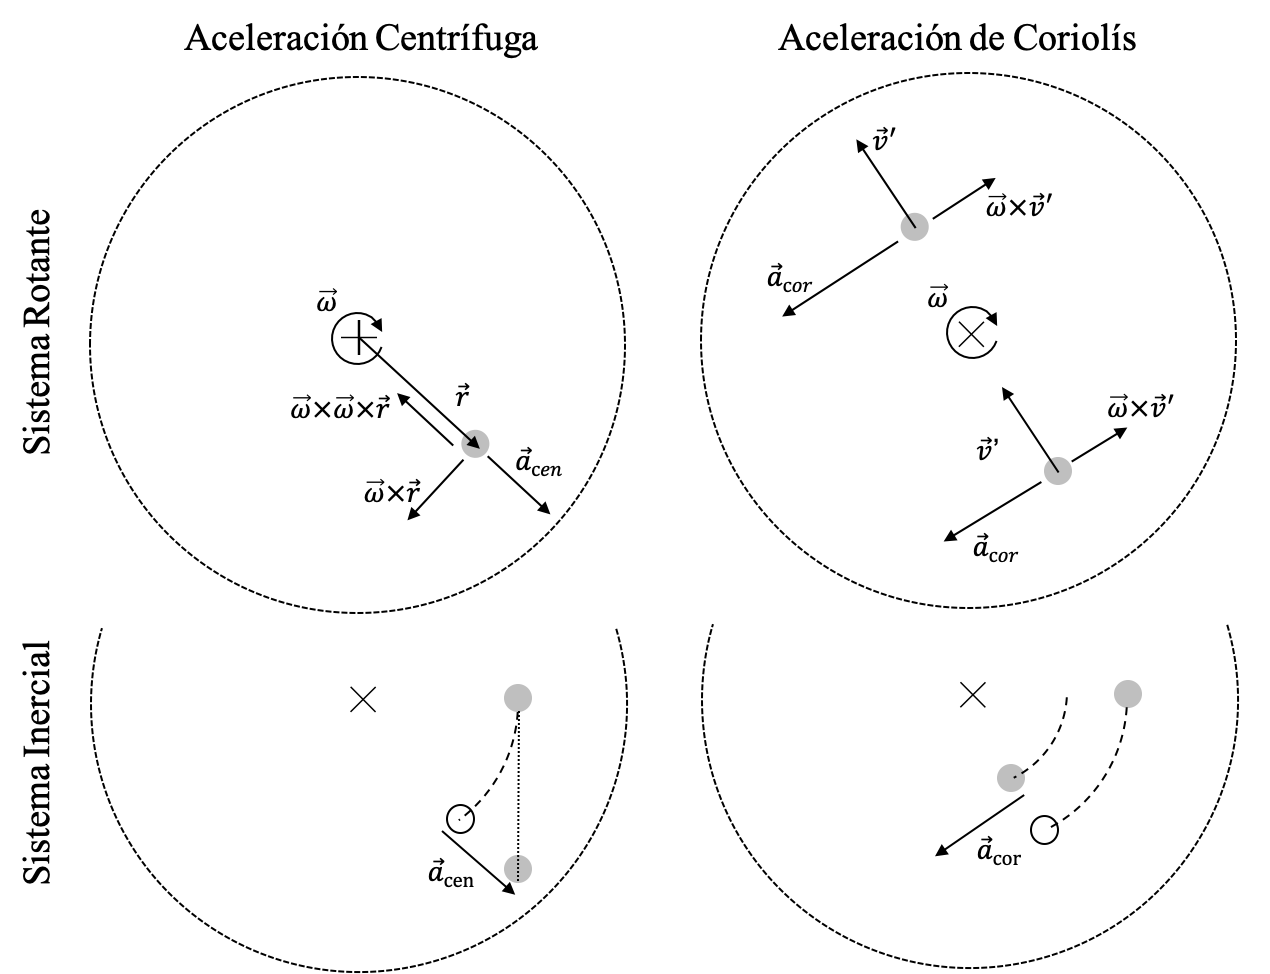
\includegraphics[width=1.0\textwidth]{./figures/square_aceleraciones_ficticias.png}
\caption{Explicación esquemática del origen y dirección de las
aceleraciones centrífuga y de
Coriolís.\label{fig:aceleraciones_ficticias}}
\end{figure}

\begin{itemize}
\tightlist
\item
  \(\vec{a}_\mathrm{cen}=-\vec\omega\times(\vec\omega\times\vec r')\).
  Esta aceleración apunta siempre en dirección contraria al eje de
  rotación (ver diagrama superior izquierdo en la
  \autoref{fig:aceleraciones_ficticias}). Por la misma razón se conoce
  como \textbf{aceleración centrífuga}. En términos inerciales, la
  aceleración centrífuga es una manifestación de la tendencia de las
  partículas a mantener su dirección de movimiento (ver diagrama
  inferior izquierdo en la \autoref{fig:aceleraciones_ficticias}). Visto
  desde el sistema rotante esta condición se manifiesta como una
  tendencia de las partículas a alejarse del eje de rotación.
\end{itemize}

\begin{itemize}
\tightlist
\item
  \(\vec{a}_\mathrm{cor}=-2\vec\omega\times\vec v'\). Esta aceleración
  apunta siempre en dirección perpendicular a la velocidad de la
  partícula (medida en el sistema rotante) y puede ser contraria o en el
  mismo sentido a la dirección de rotación del sistema de referencia
  (ver diagrama superior derecho en la
  \autoref{fig:aceleraciones_ficticias}). Por razones históricas se
  conoce esta aceleración ficticia como \textbf{aceleración de Laplace}
  o más frecuentemente como \textbf{aceleración de Coriolís} (¡atención
  al acento final!) en honor al matemático y científico francés
  Gaspard-Gustave Coriolis
  (\hreffoot{https://forvo.com/search/Gaspard-Gustave\%20Coriolis/fr/}{``Coriolís''},
  ver recuardo \emph{Un poco de historia: Coriolís y la aceleración sin
  nombre}). En términos inerciales, la aceleración de Coriolís es una
  manifestación de la tendencia de los cuerpos a mantener su velocidad
  de rotación al cambiar a puntos del sistema que se mueven con
  velocidad diferente (ver diagrama superior derecho en la
  \autoref{fig:aceleraciones_ficticias}). Si el cuerpo esta en reposo en
  el sistema rotante \(\vec v'=\vec o\), no habrá ninguna aceleración de
  Coriolís. Si el cuerpo se mueve en dirección a puntos que rotan más
  lentamente (\(\vec v'\) apunta en dirección al eje de rotación como en
  la parte inferior derecho de la \autoref{fig:aceleraciones_ficticias})
  la partícula tiende a adelantarse. Al contrario, si la partícula se
  mueve a puntos del sistema que se mueven más rápidamente (\(\vec v'\)
  dirigida hacia afuera), la partícula tenderá a retrasarse.
\end{itemize}

\begin{itemize}
\tightlist
\item
  \(\vec{a}_\mathrm{euler}=-\dot{\vec{\omega}}\times \vec r'\). Esta
  aceleración se produce únicamente si la velocidad angular del sistema
  rotante cambia de magnitud. Por razones históricas se conoce como
  \textbf{aceleración de Euler}. En términos inerciales, la aceleración
  de Euler es una manifestación de la tendencia de los cuerpos a
  mantener la velocidad angular que traía el sistema rotante justo un
  instante antes. Así, si la aceleración angular aumenta, los cuerpos
  tenderán a retrasarse (a conservar la velocidad menor que traían) y su
  aceleración se producirá en dirección contraria a la dirección de
  rotación. Al contrario, si la aceleración angular disminuye, los
  cuerpos tenderán a acelerarse en la dirección de la rotación.
\end{itemize}
\begin{box_history}{Un poco de historia}{}{nofloat}
\small

\textbf{Coriolís y la aceleración sin nombre.} La historia del
descubrimiento de la que llamamos hoy la \emph{aceleración de Coriolís}
es una de las más curiosas e interesantes de la historia de la mecánica
\cite{Graney2011},\cite{Gerkema2012}

Hoy sabemos que el efecto de esta aceleración sobre el movimiento de
cuerpos en la superficie de una Tierra en rotación, fue descrito por
primera vez en 1651 en el libro \emph{Almagestum Novum} del astrónomo
italiano \textbf{Giovanni Battista Riccioli} (``Richioli'').

Con el propósito de probar que la Tierra no rotaba (Riccioli apoyaba una
forma de teoría geocéntrica), el astrónomo italiano propuso el siguiente
experimento mental: láncese un proyectil desde un punto en el ecuador de
una Tierra que rota en dirección al norte. ¿Caerá el proyectil sobre el
meridiano del lugar desde el que fue lanzado?

La respuesta ofrecida por Riccioli utiliza un razonamiento similar a
aquel que aparece representado en el diagrama abajo a la derecha en la
\autoref{fig:fuerzas_ficticias}. Si la Tierra rota, el cañón en el
ecuador se moverá (respecto a un sistema inercial externo) hacia el
oriente, más rápido que cualquier punto en una latitud mayor (más cerca
al eje de rotación). De este modo, al avanzar hacia el norte el
proyectil irá sobrepasando (por su velocidad mayor) los puntos de la
superficie que están debajo de él. Al final, la bala caerá al oriente
del meridiano desde el que fue lanzado. En términos modernos, el
proyectil sufré una aceleración que va en la misma dirección de rotación
de la Tierra (hacia el oriente).

Como el efecto no había sido observado hasta la fecha, Riccioli pensó
que se trataba de un poderoso argumento en contra de la idea de una
Tierra en rotación. Curiosamente (y sin proponérselo), miembros de la
\emph{Accademia del Cimento} en Italia, observaron pocos años después la
aceleración anómala descrita por Riccioli al estudiar el movimiento de
péndulos. Y es que el cuerpo suspendido en el péndulo se comporta como
una bala de cañón. Si suponemos que oscila inicialmente moviéndose del
ecuador hacia el norte la tendencia a desplazarse al oriente hará que el
plano de oscilación cambie en el sentido de las manecillas del reloj. En
las notas de la academia de la década de 1660 quedo registrado la
observación sistemática de este efecto. Los académicos no pudieron
explicar el fenómeno pero tampoco lograron asociarlo con la ``predicción
de Riccioli''. No fue sino hasta 1851 cuando el mismo experimento fue
repetido bajo condiciones controladas (y con el conocimiento pleno de la
existencia de la aceleración anómala descrita por Riccioli) por el
astrónomo francés León Foucault
(\hreffoot{https://forvo.com/word/l\%C3\%A9on_foucault/\#fr}{``Fuco''}).

La misma aceleración análoga predicha originalmente por Riccioli fue
descrita para distintas condiciones (cuerpos en caída libre, cuerpos
lanzados hacia arriba, cuerpos lanzados hacia el oriente) en trabajos
posteriores durante el mismo siglo por astrónomos y físicos como
Giovanni Borelli (1668), Claude Dechales (1674) e incluso el mismo Isaac
Newton en camino a su formulación de la teoría de gravitación universal
(1680).

Una teoría rigurosa y completa de esta aceleración anómala solo llegó a
ser formulada hasta 1798 por Pierre-Simon Laplace, quién la presento
como parte de su obra cumpre \emph{Tratado de Mecánica Celeste} y en
relación con su estudio del fenómeno de las mareas lunisolares. La
descripción de Laplace fue tan completa que para hacer justicia
deberíamos llamar a esta la \textbf{aceleración de Laplace}.

En el año 1835, el matemático y científico francés Gaspard-Gustave
Coriolis, en un artículo en francés titulado ``\emph{Disertación sobre
las ecuaciones de movimiento relativo de los sistemas corporales}''
\cite{Coriolis1835}, presentó la formula general que dedujimos en esta
sección para \(\vec a_\mathrm{cor}\) y a la que llamo ``fuerza
centrífuga compuesta''. El objetivo de Corilís erá estudiar las
distintas aceleraciones ficticias que se producen en los fluídos en
sistemas mecánicos en rotación (tales como las ruedas de molino movidas
por agua).

Si bien el resultado de Corilís no atrajo mucho la atención por al menos
cuatrro décadas, no fue sino hasta 1879 cuando algunos físicos,
estudiando problemas mecánicos locales, incluyendo el péndulo de
Foucault, empezaron a identificar esta aceleración con el nombre de
Coriolís. Ya para el año 1912, y en el contexto de trabajos relacionados
con las fuerzas dentro de fluídos en movimiento, la aceleración era
conocida en la literatura como \textbf{aceleración de Coriolís} o
\textbf{Fuerza de Coriolís}.

\end{box_history}
\begin{figure}[t]
\centering
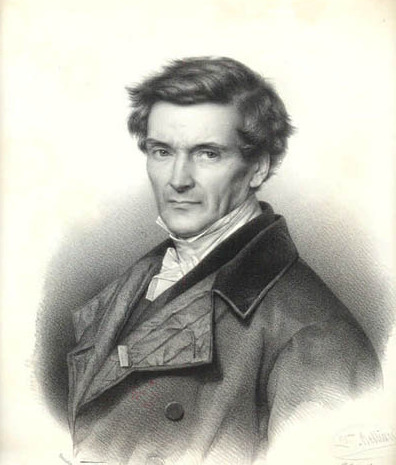
\includegraphics[width=0.5\textwidth]{./figures/vertical_coriolis.png}
\caption{Gaspard-Gustave Coriolis (1792-1843) en un retrato de 1841.
Coriolís tuvo la suerte de que una de las más importantes aceleraciones
ficticias que se producen en sistemas en rotación, y que habían sido
identificada y descritas antes por varios físicos desde Laplace hasta
Riccioli, llevara finalmente su nombre.\label{fig:coriolis}}
\end{figure}



\hypertarget{ejemplo_numerico_rotante}{%
\subsection{Un ejemplo numérico}\label{ejemplo_numerico_rotante}}

Para poner todo lo visto en las secciones anteriores a prueba,
construyamos primero un sistema mecánico cuya solución podamos resolver
numericamente y estudiar desde distintos sistemas de coordenadas.

Supongamos por ejemplo una partícula cuyo estado cinemático arbitrario
en un momento inicial dado es \(\vec r_0:(1,0,0)\) y
\(\vec v_0:(0,1,0)\) (en unidades arbitrarias).

Supongamos también que la partícula esta sometida a una aceleración
\(\vec a(t,\vec r,\vec v)\) (campo de aceleración) que depende en
general de la posición y la velocidad.

Tomemos el caso de interés para nuestro libro, de una aceleración (en el
sistema inercial) del tipo de aceleración gravitacional:

\[
\vec a = -k\frac{\vec r}{r^{n+1}}
\] donde \(k\) es una constante y \(n\) un exponente arbitrario (\(n=2\)
para el caso de la aceleración de la gravedad).

Podemos construir una rutina que implementa este campo de aceleraciones
(o modificarla para ver el efecto):

    \begin{code}{}{}\begin{Verbatim}[fontsize=\small,commandchars=\\\{\}]
\PY{k}{def} \PY{n+nf}{a\PYZus{}inercial}\PY{p}{(}\PY{n}{t}\PY{p}{,}\PY{n}{r}\PY{p}{,}\PY{n}{v}\PY{p}{,}\PY{n}{parametros}\PY{p}{)}\PY{p}{:}
    \PY{k+kn}{from} \PY{n+nn}{numpy}\PY{n+nn}{.}\PY{n+nn}{linalg} \PY{k}{import} \PY{n}{norm}
    \PY{n}{k}\PY{o}{=}\PY{n}{parametros}\PY{p}{[}\PY{l+s+s2}{\PYZdq{}}\PY{l+s+s2}{k}\PY{l+s+s2}{\PYZdq{}}\PY{p}{]}
    \PY{n}{n}\PY{o}{=}\PY{n}{parametros}\PY{p}{[}\PY{l+s+s2}{\PYZdq{}}\PY{l+s+s2}{n}\PY{l+s+s2}{\PYZdq{}}\PY{p}{]}
    \PY{n}{a}\PY{o}{=}\PY{o}{\PYZhy{}}\PY{n}{k}\PY{o}{*}\PY{n}{r}\PY{o}{/}\PY{n}{norm}\PY{p}{(}\PY{n}{r}\PY{p}{)}\PY{o}{*}\PY{o}{*}\PY{p}{(}\PY{n}{n}\PY{o}{+}\PY{l+m+mi}{1}\PY{p}{)}
    \PY{k}{return} \PY{n}{a}
\end{Verbatim}

%%

\end{code}

Usando los métodos vistos en la \autoref{integracion_numerica_edm}
podemos resolver la ecuación de movimiento en el sistema de referencia
inercial. Para ello debemos escribir primero la rutina que implementa la
ecuación de movimiento linearizada (como vimos en el
\autoref{code:edm_ejemplo1}):

    \begin{code}{}{}\begin{Verbatim}[fontsize=\small,commandchars=\\\{\}]
\PY{k}{def} \PY{n+nf}{edm\PYZus{}sistema\PYZus{}general}\PY{p}{(}\PY{n}{Y}\PY{p}{,}\PY{n}{t}\PY{p}{,}\PY{n}{aceleracion}\PY{p}{,}\PY{n}{parametros}\PY{p}{)}\PY{p}{:}
    \PY{k+kn}{from} \PY{n+nn}{numpy} \PY{k}{import} \PY{n}{zeros}
    \PY{n}{dYdt}\PY{o}{=}\PY{n}{zeros}\PY{p}{(}\PY{l+m+mi}{6}\PY{p}{)}
    
    \PY{n}{dYdt}\PY{p}{[}\PY{p}{:}\PY{l+m+mi}{3}\PY{p}{]}\PY{o}{=}\PY{n}{Y}\PY{p}{[}\PY{l+m+mi}{3}\PY{p}{:}\PY{p}{]}
    \PY{n}{dYdt}\PY{p}{[}\PY{l+m+mi}{3}\PY{p}{:}\PY{p}{]}\PY{o}{=}\PY{n}{aceleracion}\PY{p}{(}\PY{n}{t}\PY{p}{,}\PY{n}{Y}\PY{p}{[}\PY{p}{:}\PY{l+m+mi}{3}\PY{p}{]}\PY{p}{,}\PY{n}{Y}\PY{p}{[}\PY{l+m+mi}{3}\PY{p}{:}\PY{p}{]}\PY{p}{,}\PY{n}{parametros}\PY{p}{)}

    \PY{k}{return} \PY{n}{dYdt}
\end{Verbatim}

%%

\end{code}

La solución numérica a la ecuación de movimiento se obtiene con este
código:

    \begin{code}{}{}\begin{Verbatim}[fontsize=\small,commandchars=\\\{\}]
\PY{c+c1}{\PYZsh{}Condiciones iniciales}
\PY{k+kn}{from} \PY{n+nn}{numpy} \PY{k}{import} \PY{n}{array}\PY{p}{,}\PY{n}{concatenate}
\PY{n}{ro\PYZus{}ine}\PY{o}{=}\PY{n}{array}\PY{p}{(}\PY{p}{[}\PY{l+m+mf}{1.0}\PY{p}{,}\PY{l+m+mf}{0.0}\PY{p}{,}\PY{l+m+mf}{0.0}\PY{p}{]}\PY{p}{)}
\PY{n}{vo\PYZus{}ine}\PY{o}{=}\PY{n}{array}\PY{p}{(}\PY{p}{[}\PY{l+m+mf}{0.0}\PY{p}{,}\PY{l+m+mf}{0.5}\PY{p}{,}\PY{l+m+mf}{0.0}\PY{p}{]}\PY{p}{)}
\PY{n}{Yos}\PY{o}{=}\PY{n}{concatenate}\PY{p}{(}\PY{p}{(}\PY{n}{ro\PYZus{}ine}\PY{p}{,}\PY{n}{vo\PYZus{}ine}\PY{p}{)}\PY{p}{)}

\PY{c+c1}{\PYZsh{}Parametros}
\PY{n}{parametros}\PY{o}{=}\PY{n+nb}{dict}\PY{p}{(}\PY{n}{k}\PY{o}{=}\PY{l+m+mi}{1}\PY{p}{,}\PY{n}{n}\PY{o}{=}\PY{l+m+mi}{2}\PY{p}{,}\PY{n}{omega0}\PY{o}{=}\PY{l+m+mf}{0.3}\PY{p}{)}

\PY{c+c1}{\PYZsh{}Tiempos para la integración}
\PY{k+kn}{from} \PY{n+nn}{numpy} \PY{k}{import} \PY{n}{linspace}
\PY{n}{Nt}\PY{o}{=}\PY{l+m+mi}{1000}
\PY{n}{ts}\PY{o}{=}\PY{n}{linspace}\PY{p}{(}\PY{l+m+mi}{0}\PY{p}{,}\PY{l+m+mi}{10}\PY{p}{,}\PY{n}{Nt}\PY{p}{)}

\PY{c+c1}{\PYZsh{}Solución numérica}
\PY{k+kn}{from} \PY{n+nn}{scipy}\PY{n+nn}{.}\PY{n+nn}{integrate} \PY{k}{import} \PY{n}{odeint}
\PY{n}{Ys}\PY{o}{=}\PY{n}{odeint}\PY{p}{(}\PY{n}{edm\PYZus{}sistema\PYZus{}general}\PY{p}{,}\PY{n}{Yos}\PY{p}{,}\PY{n}{ts}\PY{p}{,}\PY{n}{args}\PY{o}{=}\PY{p}{(}\PY{n}{a\PYZus{}inercial}\PY{p}{,}\PY{n}{parametros}\PY{p}{)}\PY{p}{)}
\end{Verbatim}

%%

\end{code}

Un gráfico de la solución en el plano \(x-y\) (del sistema inercial)
sería:
%%HIDE%%
    \begin{code}{Algoritmo}{code:5_Mecanica_14}\begin{Verbatim}[fontsize=\small,commandchars=\\\{\}]
\PY{k+kn}{import} \PY{n+nn}{matplotlib}\PY{n+nn}{.}\PY{n+nn}{pyplot} \PY{k}{as} \PY{n+nn}{plt}
\PY{n}{fig}\PY{o}{=}\PY{n}{plt}\PY{o}{.}\PY{n}{figure}\PY{p}{(}\PY{n}{figsize}\PY{o}{=}\PY{p}{(}\PY{l+m+mi}{5}\PY{p}{,}\PY{l+m+mi}{5}\PY{p}{)}\PY{p}{)}\PY{p}{;}
\PY{n}{ax}\PY{o}{=}\PY{n}{fig}\PY{o}{.}\PY{n}{gca}\PY{p}{(}\PY{p}{)}
\PY{n}{ax}\PY{o}{.}\PY{n}{plot}\PY{p}{(}\PY{n}{Ys}\PY{p}{[}\PY{p}{:}\PY{p}{,}\PY{l+m+mi}{0}\PY{p}{]}\PY{p}{,}\PY{n}{Ys}\PY{p}{[}\PY{p}{:}\PY{p}{,}\PY{l+m+mi}{1}\PY{p}{]}\PY{p}{,}\PY{l+s+s1}{\PYZsq{}}\PY{l+s+s1}{k\PYZhy{}}\PY{l+s+s1}{\PYZsq{}}\PY{p}{)}\PY{p}{;}
\PY{k+kn}{from} \PY{n+nn}{pymcel}\PY{n+nn}{.}\PY{n+nn}{plot} \PY{k}{import} \PY{n}{fija\PYZus{}ejes\PYZus{}proporcionales}
\PY{n}{fija\PYZus{}ejes\PYZus{}proporcionales}\PY{p}{(}\PY{n}{ax}\PY{p}{,}\PY{n}{Ys}\PY{p}{[}\PY{p}{:}\PY{p}{,}\PY{p}{:}\PY{l+m+mi}{2}\PY{p}{]}\PY{p}{,}\PY{n}{ycm}\PY{o}{=}\PY{l+m+mi}{0}\PY{p}{)}\PY{p}{;}
\end{Verbatim}

%%

\tcblower
\footnotesize
\em ver Figura \ref{fig:code:5_Mecanica_14}
\end{code}

    \begin{center}

\begin{figure}[ht!]
\centering
    \adjustimage{max size={0.8\linewidth}{0.8\paperheight}}{combined_files/combined_838_0.png}
\caption{Figura correspondiente al código \ref{code:5_Mecanica_14}.\label{fig:code:5_Mecanica_14}}
\end{figure}

    \end{center}
%{ \hspace*{\fill} \\}
    
Convirtamos primero todas las componentes de los vectores posición y
velocidad de la partícula al sistema de coordenadas rotante, aplicando
para ello una matriz de rotación (a la manera como se definión en la
\autoref{conicas_rotacion_plano}) en un ángulo igual al que han
rotado los ejes en el tiempo \(t\), esto es \(\theta=\omega_0 t\):

\[
R=
\left(
\begin{array}{ccc}
\cos(\omega_0 t) & \sin(\omega_0 t) & 0 \\
-\sin(\omega_0 t) & \cos(\omega_0 t) & 0 \\
0 & 0 & 1
\end{array}
\right)
\]

La aplicación de esta rotación a todas las posiciones y velocidades se
puede realizar con este código:

    \begin{code}{}{}\begin{Verbatim}[fontsize=\small,commandchars=\\\{\}]
\PY{c+c1}{\PYZsh{}Velocidad angular}
\PY{k+kn}{from} \PY{n+nn}{numpy} \PY{k}{import} \PY{n}{array}
\PY{n}{omega0}\PY{o}{=}\PY{n}{parametros}\PY{p}{[}\PY{l+s+s2}{\PYZdq{}}\PY{l+s+s2}{omega0}\PY{l+s+s2}{\PYZdq{}}\PY{p}{]}
\PY{n}{omega\PYZus{}vec}\PY{o}{=}\PY{n}{array}\PY{p}{(}\PY{p}{[}\PY{l+m+mi}{0}\PY{p}{,}\PY{l+m+mi}{0}\PY{p}{,}\PY{n}{omega0}\PY{p}{]}\PY{p}{)}

\PY{c+c1}{\PYZsh{}Extraemos las posiciones del vector solución}
\PY{n}{rs\PYZus{}ine}\PY{o}{=}\PY{n}{Ys}\PY{p}{[}\PY{p}{:}\PY{p}{,}\PY{p}{:}\PY{l+m+mi}{3}\PY{p}{]}
\PY{n}{vs\PYZus{}ine}\PY{o}{=}\PY{n}{Ys}\PY{p}{[}\PY{p}{:}\PY{p}{,}\PY{l+m+mi}{3}\PY{p}{:}\PY{p}{]}

\PY{c+c1}{\PYZsh{}Aquí almacenaremos las posiciones en el sistema rotante}
\PY{k+kn}{from} \PY{n+nn}{numpy} \PY{k}{import} \PY{n}{zeros\PYZus{}like}
\PY{n}{rs\PYZus{}rot}\PY{o}{=}\PY{n}{zeros\PYZus{}like}\PY{p}{(}\PY{n}{rs\PYZus{}ine}\PY{p}{)}

\PY{c+c1}{\PYZsh{}Aquí realizamos las rotaciones}
\PY{k}{for} \PY{n}{i} \PY{o+ow}{in} \PY{n+nb}{range}\PY{p}{(}\PY{n}{Nt}\PY{p}{)}\PY{p}{:}
    
    \PY{c+c1}{\PYZsh{}Matriz de rotación}
    \PY{k+kn}{from} \PY{n+nn}{spiceypy} \PY{k}{import} \PY{n}{rotate}
    \PY{n}{R}\PY{o}{=}\PY{n}{rotate}\PY{p}{(}\PY{n}{omega0}\PY{o}{*}\PY{n}{ts}\PY{p}{[}\PY{n}{i}\PY{p}{]}\PY{p}{,}\PY{l+m+mi}{3}\PY{p}{)}
    
    \PY{c+c1}{\PYZsh{}Rotación del vector posición y el vector velocidad}
    \PY{k+kn}{from} \PY{n+nn}{spiceypy} \PY{k}{import} \PY{n}{mxv}
    \PY{n}{rs\PYZus{}rot}\PY{p}{[}\PY{n}{i}\PY{p}{]}\PY{o}{=}\PY{n}{mxv}\PY{p}{(}\PY{n}{R}\PY{p}{,}\PY{n}{rs\PYZus{}ine}\PY{p}{[}\PY{n}{i}\PY{p}{]}\PY{p}{)}
\end{Verbatim}

%%

\end{code}

Un gráfico de la posición en el sistema rotante se vería así:

    \begin{code}{Algoritmo}{code:plot_rotating_frame}\begin{Verbatim}[fontsize=\small,commandchars=\\\{\}]
\PY{k+kn}{import} \PY{n+nn}{matplotlib}\PY{n+nn}{.}\PY{n+nn}{pyplot} \PY{k}{as} \PY{n+nn}{plt}
\PY{n}{fig}\PY{o}{=}\PY{n}{plt}\PY{o}{.}\PY{n}{figure}\PY{p}{(}\PY{n}{figsize}\PY{o}{=}\PY{p}{(}\PY{l+m+mi}{5}\PY{p}{,}\PY{l+m+mi}{5}\PY{p}{)}\PY{p}{)}\PY{p}{;}
\PY{n}{ax}\PY{o}{=}\PY{n}{fig}\PY{o}{.}\PY{n}{gca}\PY{p}{(}\PY{p}{)}
\PY{n}{ax}\PY{o}{.}\PY{n}{plot}\PY{p}{(}\PY{n}{rs\PYZus{}rot}\PY{p}{[}\PY{p}{:}\PY{p}{,}\PY{l+m+mi}{0}\PY{p}{]}\PY{p}{,}\PY{n}{rs\PYZus{}rot}\PY{p}{[}\PY{p}{:}\PY{p}{,}\PY{l+m+mi}{1}\PY{p}{]}\PY{p}{,}\PY{l+s+s1}{\PYZsq{}}\PY{l+s+s1}{k\PYZhy{}}\PY{l+s+s1}{\PYZsq{}}\PY{p}{)}\PY{p}{;}
\PY{k+kn}{from} \PY{n+nn}{pymcel}\PY{n+nn}{.}\PY{n+nn}{plot} \PY{k}{import} \PY{n}{fija\PYZus{}ejes\PYZus{}proporcionales}
\PY{n}{fija\PYZus{}ejes\PYZus{}proporcionales}\PY{p}{(}\PY{n}{ax}\PY{p}{,}\PY{n}{rs\PYZus{}rot}\PY{p}{)}\PY{p}{;}
\end{Verbatim}

%%

\tcblower
\footnotesize
\em ver Figura \ref{fig:code:plot_rotating_frame}
\end{code}

    \begin{center}

\begin{figure}[ht!]
\centering
    \adjustimage{max size={0.8\linewidth}{0.8\paperheight}}{combined_files/combined_843_0.png}
\caption{Figura correspondiente al código \ref{code:plot_rotating_frame}.\label{fig:code:plot_rotating_frame}}
\end{figure}

    \end{center}
%{ \hspace*{\fill} \\}
    
Como es de esperarse la precesión de la trayectoria en el sentido de las
manecillas del reloj, es debida a que los ejes del sistema no inercial
rotan en la dirección opuesta. En el sistema de referencia no inercial,
el movimiento en realidad es el producto de la acción de nuevas
aceleraciones.

Calculemos ahora otras cantidades cinemáticas en el movimiento de la
partícula, tal y como son medida en el sistema de referencia rotante.
Por ejemplo la velocidad. Para ello usemos la definición misma de
velocidad media, \(\vec v'\approx\Delta \vec r'/\Delta t\):

    \begin{code}{}{}\begin{Verbatim}[fontsize=\small,commandchars=\\\{\}]
\PY{n}{vs\PYZus{}rot\PYZus{}num}\PY{o}{=}\PY{n}{zeros\PYZus{}like}\PY{p}{(}\PY{n}{rs\PYZus{}rot}\PY{p}{)}
\PY{k}{for} \PY{n}{i} \PY{o+ow}{in} \PY{n+nb}{range}\PY{p}{(}\PY{l+m+mi}{1}\PY{p}{,}\PY{n}{Nt}\PY{p}{)}\PY{p}{:}
    \PY{n}{vs\PYZus{}rot\PYZus{}num}\PY{p}{[}\PY{n}{i}\PY{p}{]}\PY{o}{=}\PY{p}{(}\PY{n}{rs\PYZus{}rot}\PY{p}{[}\PY{n}{i}\PY{p}{]}\PY{o}{\PYZhy{}}\PY{n}{rs\PYZus{}rot}\PY{p}{[}\PY{n}{i}\PY{o}{\PYZhy{}}\PY{l+m+mi}{1}\PY{p}{]}\PY{p}{)}\PY{o}{/}\PY{p}{(}\PY{n}{ts}\PY{p}{[}\PY{n}{i}\PY{p}{]}\PY{o}{\PYZhy{}}\PY{n}{ts}\PY{p}{[}\PY{n}{i}\PY{o}{\PYZhy{}}\PY{l+m+mi}{1}\PY{p}{]}\PY{p}{)}
\end{Verbatim}

%%

\end{code}
\vspace{-1em}

%%hidecode


    \begin{Verbatim}[fontsize=\small,commandchars=\\\{\}]
Velocidad en el sistema rotante (numérica):
[[-0.08  0.2 ]
 [-0.16  0.21]
 [-0.24  0.21]
 [-0.33  0.22]
 [-0.42  0.23]
 [-0.53  0.25]
 [-0.65  0.26]
 [-0.79  0.27]
 [-0.96  0.26]]
\end{Verbatim}

Comparemos la velocidad calculada de esta manera y aquella que obtenemos
con la relación teórica expresada por la Ec.
(\ref{eq:adicion_velocidades_rotante}):

    \begin{code}{}{}\begin{Verbatim}[fontsize=\small,commandchars=\\\{\}]
\PY{n}{vs\PYZus{}rot\PYZus{}teo}\PY{o}{=}\PY{n}{zeros\PYZus{}like}\PY{p}{(}\PY{n}{rs\PYZus{}rot}\PY{p}{)}
\PY{k}{for} \PY{n}{i} \PY{o+ow}{in} \PY{n+nb}{range}\PY{p}{(}\PY{l+m+mi}{1}\PY{p}{,}\PY{n}{Nt}\PY{p}{)}\PY{p}{:}
    \PY{k+kn}{from} \PY{n+nn}{spiceypy} \PY{k}{import} \PY{n}{mxv}\PY{p}{,}\PY{n}{vcrss}
    \PY{n}{R}\PY{o}{=}\PY{n}{rotate}\PY{p}{(}\PY{n}{omega0}\PY{o}{*}\PY{n}{ts}\PY{p}{[}\PY{n}{i}\PY{p}{]}\PY{p}{,}\PY{l+m+mi}{3}\PY{p}{)}
    \PY{n}{vs\PYZus{}rot\PYZus{}teo}\PY{p}{[}\PY{n}{i}\PY{p}{]}\PY{o}{=}\PY{n}{mxv}\PY{p}{(}\PY{n}{R}\PY{p}{,}\PY{n}{vs\PYZus{}ine}\PY{p}{[}\PY{n}{i}\PY{p}{]}\PY{o}{\PYZhy{}}\PY{n}{vcrss}\PY{p}{(}\PY{n}{omega\PYZus{}vec}\PY{p}{,}\PY{n}{rs\PYZus{}ine}\PY{p}{[}\PY{n}{i}\PY{p}{]}\PY{p}{)}\PY{p}{)}
\end{Verbatim}

%%

\end{code}
\vspace{-1em}

%%hidecode


    \begin{Verbatim}[fontsize=\small,commandchars=\\\{\}]
Velocidad en el sistema rotante (teórica):
[[-0.08  0.2 ]
 [-0.16  0.21]
 [-0.24  0.21]
 [-0.33  0.22]
 [-0.43  0.23]
 [-0.53  0.25]
 [-0.65  0.26]
 [-0.79  0.27]
 [-0.97  0.26]]
\end{Verbatim}

Que coincide (dentro de los errores numéricos) con la velocidad
calculada con el procedimiento aproximado. Esta es pues, una manera de
comprobar la validez de la Ec. (\ref{eq:adicion_velocidades_rotante}) y
al mismo tiempo reconocer que su uso no es enteramente trivial.

Comparemos ahora las aceleraciones calculadas numéricamente y de acuerdo
con lo esperado por la Ec. (\ref{eq:ley_adicion_aceleraciones}):

    \begin{code}{}{}\begin{Verbatim}[fontsize=\small,commandchars=\\\{\}]
\PY{n}{as\PYZus{}rot\PYZus{}num}\PY{o}{=}\PY{n}{zeros\PYZus{}like}\PY{p}{(}\PY{n}{rs\PYZus{}rot}\PY{p}{)}
\PY{n}{as\PYZus{}rot\PYZus{}teo}\PY{o}{=}\PY{n}{zeros\PYZus{}like}\PY{p}{(}\PY{n}{rs\PYZus{}rot}\PY{p}{)}

\PY{k}{for} \PY{n}{i} \PY{o+ow}{in} \PY{n+nb}{range}\PY{p}{(}\PY{l+m+mi}{1}\PY{p}{,}\PY{n}{Nt}\PY{p}{)}\PY{p}{:}
    \PY{k+kn}{from} \PY{n+nn}{spiceypy} \PY{k}{import} \PY{n}{mxv}\PY{p}{,}\PY{n}{vcrss}
    \PY{n}{R}\PY{o}{=}\PY{n}{rotate}\PY{p}{(}\PY{n}{omega0}\PY{o}{*}\PY{n}{ts}\PY{p}{[}\PY{n}{i}\PY{p}{]}\PY{p}{,}\PY{l+m+mi}{3}\PY{p}{)}
    
    \PY{c+c1}{\PYZsh{}Aceleración numérica}
    \PY{n}{as\PYZus{}rot\PYZus{}num}\PY{p}{[}\PY{n}{i}\PY{p}{]}\PY{o}{=}\PY{p}{(}\PY{n}{vs\PYZus{}rot\PYZus{}num}\PY{p}{[}\PY{n}{i}\PY{p}{]}\PY{o}{\PYZhy{}}\PY{n}{vs\PYZus{}rot\PYZus{}num}\PY{p}{[}\PY{n}{i}\PY{o}{\PYZhy{}}\PY{l+m+mi}{1}\PY{p}{]}\PY{p}{)}\PY{o}{/}\PY{p}{(}\PY{n}{ts}\PY{p}{[}\PY{n}{i}\PY{p}{]}\PY{o}{\PYZhy{}}\PY{n}{ts}\PY{p}{[}\PY{n}{i}\PY{o}{\PYZhy{}}\PY{l+m+mi}{1}\PY{p}{]}\PY{p}{)}
    
    \PY{c+c1}{\PYZsh{}Aceleración inercial (en el sistema inercial de referencia)}
    \PY{n}{a\PYZus{}ine}\PY{o}{=}\PY{n}{a\PYZus{}inercial}\PY{p}{(}\PY{n}{ts}\PY{p}{[}\PY{n}{i}\PY{p}{]}\PY{p}{,}\PY{n}{rs\PYZus{}ine}\PY{p}{[}\PY{n}{i}\PY{p}{]}\PY{p}{,}\PY{n}{vs\PYZus{}ine}\PY{p}{[}\PY{n}{i}\PY{p}{]}\PY{p}{,}\PY{n}{parametros}\PY{p}{)}
    
    \PY{c+c1}{\PYZsh{}Aceleración centrífuga (en el sistema inercial de referencia)}
    \PY{n}{acen\PYZus{}ine}\PY{o}{=}\PY{o}{\PYZhy{}}\PY{n}{vcrss}\PY{p}{(}\PY{n}{omega\PYZus{}vec}\PY{p}{,}\PY{n}{vcrss}\PY{p}{(}\PY{n}{omega\PYZus{}vec}\PY{p}{,}\PY{n}{rs\PYZus{}ine}\PY{p}{[}\PY{n}{i}\PY{p}{]}\PY{p}{)}\PY{p}{)}
    
    \PY{c+c1}{\PYZsh{}Aceleración de Coriolis (en el sistema inercial de referencia)}
    \PY{n}{acor\PYZus{}ine}\PY{o}{=}\PY{o}{\PYZhy{}}\PY{l+m+mi}{2}\PY{o}{*}\PY{n}{vcrss}\PY{p}{(}\PY{n}{omega\PYZus{}vec}\PY{p}{,}\PY{n}{vs\PYZus{}ine}\PY{p}{[}\PY{n}{i}\PY{p}{]}\PY{p}{)}
    
    \PY{c+c1}{\PYZsh{}Aceleración en el sistema rotante}
    \PY{n}{as\PYZus{}rot\PYZus{}teo}\PY{p}{[}\PY{n}{i}\PY{p}{]}\PY{o}{=}\PY{n}{mxv}\PY{p}{(}\PY{n}{R}\PY{p}{,}\PY{n}{a\PYZus{}ine}\PY{o}{+}\PY{n}{acen\PYZus{}ine}\PY{o}{+}\PY{n}{acor\PYZus{}ine}\PY{p}{)}
\end{Verbatim}

%%

\end{code}
\vspace{-1em}

%%hidecode


    \begin{Verbatim}[fontsize=\small,commandchars=\\\{\}]
Aceleracion en el sistema rotante (numérica):
[[-0.8   0.03]
 [-0.82  0.05]
 [-0.85  0.08]
 [-0.91  0.1 ]
 [-0.99  0.12]
 [-1.1   0.13]
 [-1.27  0.11]
 [-1.51  0.05]
 [-1.89 -0.09]]
Aceleracion en el sistema rotante (teórica):
[[-0.62  0.03]
 [-0.64  0.06]
 [-0.68  0.09]
 [-0.74  0.12]
 [-0.83  0.14]
 [-0.96  0.15]
 [-1.14  0.14]
 [-1.41  0.08]
 [-1.83 -0.08]]
\end{Verbatim}

Con estos elementos a la mano, podemos ahora probar resolver las
ecuaciones de movimiento de la partícula, pero en el sistema rotante, y
comparar el resultado con el obtenido en la
\autoref{fig:code:plot_rotating_frame}. Para ello lo único que tenemos
que hacer es escribir una rutina que nos de las componentes del campo de
aceleración \(\vec a(\vec r,\vec v)\) pero en el sistema rotante:

    \begin{code}{}{}\begin{Verbatim}[fontsize=\small,commandchars=\\\{\}]
\PY{k}{def} \PY{n+nf}{a\PYZus{}rotante}\PY{p}{(}\PY{n}{t}\PY{p}{,}\PY{n}{r}\PY{p}{,}\PY{n}{v}\PY{p}{,}\PY{n}{parametros}\PY{p}{)}\PY{p}{:}
    
    \PY{n}{omega0}\PY{o}{=}\PY{n}{parametros}\PY{p}{[}\PY{l+s+s2}{\PYZdq{}}\PY{l+s+s2}{omega0}\PY{l+s+s2}{\PYZdq{}}\PY{p}{]}
    
    \PY{k+kn}{from} \PY{n+nn}{spiceypy} \PY{k}{import} \PY{n}{rotate}\PY{p}{,}\PY{n}{mxv}\PY{p}{,}\PY{n}{vcrss}\PY{p}{,}\PY{n}{invert}
    \PY{n}{R}\PY{o}{=}\PY{n}{rotate}\PY{p}{(}\PY{n}{omega0}\PY{o}{*}\PY{n}{t}\PY{p}{,}\PY{l+m+mi}{3}\PY{p}{)} 
    
    \PY{c+c1}{\PYZsh{}Primero convierte r,v al sistema inercial}
    \PY{n}{r\PYZus{}ine}\PY{o}{=}\PY{n}{mxv}\PY{p}{(}\PY{n}{invert}\PY{p}{(}\PY{n}{R}\PY{p}{)}\PY{p}{,}\PY{n}{r}\PY{p}{)}
    \PY{n}{v\PYZus{}ine}\PY{o}{=}\PY{n}{mxv}\PY{p}{(}\PY{n}{invert}\PY{p}{(}\PY{n}{R}\PY{p}{)}\PY{p}{,}\PY{n}{v}\PY{p}{)}
    
    \PY{c+c1}{\PYZsh{}Calcula la aceleración en el sistema inercial}
    \PY{n}{ainercial}\PY{o}{=}\PY{n}{a\PYZus{}inercial}\PY{p}{(}\PY{n}{t}\PY{p}{,}\PY{n}{r\PYZus{}ine}\PY{p}{,}\PY{n}{v\PYZus{}ine}\PY{p}{,}\PY{n}{parametros}\PY{p}{)}

    \PY{c+c1}{\PYZsh{}Rota la aceleración inercial a los ejes rotantes}
    \PY{n}{ainercial\PYZus{}rot}\PY{o}{=}\PY{n}{mxv}\PY{p}{(}\PY{n}{R}\PY{p}{,}\PY{n}{ainercial}\PY{p}{)}
    
    \PY{c+c1}{\PYZsh{}Calcular la aceleración en el sistema rotante}
    \PY{n}{acen\PYZus{}rot}\PY{o}{=}\PY{o}{\PYZhy{}}\PY{n}{vcrss}\PY{p}{(}\PY{n}{omega\PYZus{}vec}\PY{p}{,}\PY{n}{vcrss}\PY{p}{(}\PY{n}{omega\PYZus{}vec}\PY{p}{,}\PY{n}{r}\PY{p}{)}\PY{p}{)}
    \PY{n}{acor\PYZus{}rot}\PY{o}{=}\PY{o}{\PYZhy{}}\PY{l+m+mi}{2}\PY{o}{*}\PY{n}{vcrss}\PY{p}{(}\PY{n}{omega\PYZus{}vec}\PY{p}{,}\PY{n}{v}\PY{p}{)}
    \PY{n}{a\PYZus{}rot}\PY{o}{=}\PY{n}{ainercial\PYZus{}rot}\PY{o}{+}\PY{n}{acen\PYZus{}rot}\PY{o}{+}\PY{n}{acor\PYZus{}rot}
    \PY{k}{return} \PY{n}{a\PYZus{}rot}
\end{Verbatim}

%%

\end{code}

La solución a la ecuación diferencial se consigue de forma analoga a
cómo lo hicimos en el caso del sistema inercial:

    \begin{code}{Algoritmo}{code:5_Mecanica_15}\begin{Verbatim}[fontsize=\small,commandchars=\\\{\}]
\PY{c+c1}{\PYZsh{}Convertimos las condiciones iniciales, al sistema rotante}
\PY{k+kn}{from} \PY{n+nn}{spiceypy} \PY{k}{import} \PY{n}{rotate}\PY{p}{,}\PY{n}{mxv}
\PY{n}{ro\PYZus{}rot}\PY{o}{=}\PY{n}{ro\PYZus{}ine}
\PY{n}{R}\PY{o}{=}\PY{n}{rotate}\PY{p}{(}\PY{l+m+mf}{0.0}\PY{p}{,}\PY{l+m+mi}{3}\PY{p}{)}
\PY{n}{vo\PYZus{}rot}\PY{o}{=}\PY{n}{mxv}\PY{p}{(}\PY{n}{R}\PY{p}{,}\PY{n}{vo\PYZus{}ine}\PY{o}{\PYZhy{}}\PY{n}{vcrss}\PY{p}{(}\PY{n}{omega\PYZus{}vec}\PY{p}{,}\PY{n}{ro\PYZus{}ine}\PY{p}{)}\PY{p}{)}

\PY{c+c1}{\PYZsh{}Condiciones iniciales}
\PY{k+kn}{from} \PY{n+nn}{numpy} \PY{k}{import} \PY{n}{concatenate}
\PY{n}{Yos\PYZus{}rot}\PY{o}{=}\PY{n}{concatenate}\PY{p}{(}\PY{p}{(}\PY{n}{ro\PYZus{}rot}\PY{p}{,}\PY{n}{vo\PYZus{}rot}\PY{p}{)}\PY{p}{)}

\PY{c+c1}{\PYZsh{}Tiempos para la integración}
\PY{k+kn}{from} \PY{n+nn}{numpy} \PY{k}{import} \PY{n}{linspace}
\PY{n}{Nt}\PY{o}{=}\PY{l+m+mi}{1000}
\PY{n}{ts}\PY{o}{=}\PY{n}{linspace}\PY{p}{(}\PY{l+m+mi}{0}\PY{p}{,}\PY{l+m+mi}{10}\PY{p}{,}\PY{n}{Nt}\PY{p}{)}

\PY{c+c1}{\PYZsh{}Solución numérica}
\PY{k+kn}{from} \PY{n+nn}{scipy}\PY{n+nn}{.}\PY{n+nn}{integrate} \PY{k}{import} \PY{n}{odeint}
\PY{n}{Ys\PYZus{}rot}\PY{o}{=}\PY{n}{odeint}\PY{p}{(}\PY{n}{edm\PYZus{}sistema\PYZus{}general}\PY{p}{,}\PY{n}{Yos\PYZus{}rot}\PY{p}{,}\PY{n}{ts}\PY{p}{,}\PY{n}{args}\PY{o}{=}\PY{p}{(}\PY{n}{a\PYZus{}rotante}\PY{p}{,}\PY{n}{parametros}\PY{p}{)}\PY{p}{)}

\PY{c+c1}{\PYZsh{}Gráfico}
\PY{k+kn}{import} \PY{n+nn}{matplotlib}\PY{n+nn}{.}\PY{n+nn}{pyplot} \PY{k}{as} \PY{n+nn}{plt}
\PY{n}{fig}\PY{o}{=}\PY{n}{plt}\PY{o}{.}\PY{n}{figure}\PY{p}{(}\PY{n}{figsize}\PY{o}{=}\PY{p}{(}\PY{l+m+mi}{5}\PY{p}{,}\PY{l+m+mi}{5}\PY{p}{)}\PY{p}{)}\PY{p}{;}
\PY{n}{ax}\PY{o}{=}\PY{n}{fig}\PY{o}{.}\PY{n}{gca}\PY{p}{(}\PY{p}{)}
\PY{n}{ax}\PY{o}{.}\PY{n}{plot}\PY{p}{(}\PY{n}{Ys\PYZus{}rot}\PY{p}{[}\PY{p}{:}\PY{p}{,}\PY{l+m+mi}{0}\PY{p}{]}\PY{p}{,}\PY{n}{Ys\PYZus{}rot}\PY{p}{[}\PY{p}{:}\PY{p}{,}\PY{l+m+mi}{1}\PY{p}{]}\PY{p}{,}\PY{l+s+s1}{\PYZsq{}}\PY{l+s+s1}{k\PYZhy{}}\PY{l+s+s1}{\PYZsq{}}\PY{p}{)}\PY{p}{;}
\PY{k+kn}{from} \PY{n+nn}{pymcel}\PY{n+nn}{.}\PY{n+nn}{plot} \PY{k}{import} \PY{n}{fija\PYZus{}ejes\PYZus{}proporcionales}
\PY{n}{fija\PYZus{}ejes\PYZus{}proporcionales}\PY{p}{(}\PY{n}{ax}\PY{p}{,}\PY{n}{Ys\PYZus{}rot}\PY{p}{[}\PY{p}{:}\PY{p}{,}\PY{p}{:}\PY{l+m+mi}{2}\PY{p}{]}\PY{p}{)}\PY{p}{;}
\end{Verbatim}

%%

\tcblower
\footnotesize
\em ver Figura \ref{fig:code:5_Mecanica_15}
\end{code}

    \begin{center}

\begin{figure}[ht!]
\centering
    \adjustimage{max size={0.8\linewidth}{0.8\paperheight}}{combined_files/combined_858_0.png}
\caption{Figura correspondiente al código \ref{code:5_Mecanica_15}.\label{fig:code:5_Mecanica_15}}
\end{figure}

    \end{center}
%{ \hspace*{\fill} \\}
    
Busque las figuras interactivas y las animaciones incluídas en el
\hreffoot{http://seap-udea.org/MecanicaCeleste_Zuluaga}{sitio en línea del
libro}.



\clearpage

\hypertarget{mecanica_problemas}{%
\section{Problemas seleccionados}\label{mecanica_problemas}}

\begin{enumerate}
\def\labelenumi{\arabic{enumi}.}
\tightlist
\item
  \textbf{Leyes de conservación.}
\end{enumerate}

\begin{quote}
\begin{enumerate}
\def\labelenumi{\alph{enumi})}
\tightlist
\item
  Demuestre que si la fuerza externa sobre un sistema de partículas es
  0, entonces el momentum total del sistema se conserva.
\end{enumerate}
\end{quote}

\begin{quote}
\begin{enumerate}
\def\labelenumi{\alph{enumi})}
\setcounter{enumi}{1}
\tightlist
\item
  Demuestre que si el torque externo sobre un sistema de partículas es
  0, entonces el momentum angular total del sistema se conserva.
\end{enumerate}
\end{quote}
\color{red}

\begin{enumerate}
\def\labelenumi{\arabic{enumi}.}
\tightlist
\item
  \textbf{Solución}.
\end{enumerate}

\begin{quote}
Está literalmente en la las notas, en la sección \textbf{Dinámica de un
sistema de partículas}.
\end{quote}

\color{black}
\begin{enumerate}
\def\labelenumi{\arabic{enumi}.}
\setcounter{enumi}{1}
\tightlist
\item
  \textbf{Lanzamiento de un proyectil.} Un proyectil de masa \(m\) es
  disparado desde la superficie de la Tierra bajo un ángulo \(\alpha\)
  desde la vertical como se muestra en la figura. La velocidad inicial
  \(v_0\) es igual a \(\sqrt[]{GM_e/R_e}\), donde \(M_e\) es la masa de
  la Tierra y \(R_e\) es su radio. ¿Qué tan alto sube el proyectil?
  Desprecie el aire resistencia y la rotación de la Tierra.
  (\emph{Ayuda}: determine qué cantidades se conservan ---¡explique
  claramente porqué!--- y aplique las leyes de conservación de dichas
  cantidades. En algún momento de su procedimiento es posible que
  encuentre dos posibles valores matemáticos para \(r_{max}\); los dos
  parecen físicamente aceptables, así que explique claramente porqué
  solo debe escoger uno y en qué consiste el otro.)
\end{enumerate}

\begin{figure}[t!]
\centering
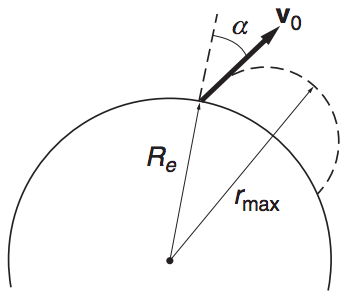
\includegraphics[width=0.5\textwidth]{./figures/problems/proyectil.png}
\caption{Geometría del lanzamiento de un proyectil desde la superficie
de una Tierra en
rotación.\label{fig:prob:lanzamiento_proyectil}}
\end{figure}
\color{red}

\begin{enumerate}
\def\labelenumi{\arabic{enumi}.}
\setcounter{enumi}{1}
\tightlist
\item
  \textbf{Solución}
\end{enumerate}

\begin{quote}
Supongamos inicialmente a la Tierra como un sista de referencia inercial
(su masa es tan grande en comparación con la del proyectil, que
práticamente no se mueve con el lanzamiento de éste). Ahora, como la
única fuerza que actúa sobre el proyectil es la fuerza gravitacional que
le hace la Tierra, que es conservativa, entonces la energía mecánica del
proyectil se conserva y podemos decir que es igual en el momento del
lanzamiento que en el punto a \(r_{max}\):
\end{quote}

\begin{quote}
\[\frac{1}{2}mv_0^2-\frac{GmM_e}{R_e}=\frac{1}{2}mv^2-\frac{GmM_e}{r_{max}},\]
\end{quote}

\begin{quote}
donde \(m\) es la masa del proyectil y \(v\) es su rapidez en
\(r_{max}\). Dado que \(v_0^2=GM_e/R_e\), la anetior ecuación se puede
simplificar a
\end{quote}

\begin{quote}
\[v^2=GM_e\left(\frac{2}{r_{max}}-\frac{1}{R_e}\right).\]
\end{quote}

\begin{quote}
Ahora, dado que la fuerza gravitacional que le hace la Tierra al
proyectil es central, no realiza ningún torque sobre éste, de forma que
su momento angular es constante durante la trayectoria y, por lo tanto,
igual en los mismos dos puntos escogidos anteriormente:
\end{quote}

\begin{quote}
\[mR_ev_0\sin\alpha = mr_{max}v\sin(\pi/2).\]
\end{quote}

\begin{quote}
Igualando ambas ecuaciones, se obtiene la ecuación cuadrática para
\(r_{max}\):
\end{quote}

\begin{quote}
\[r_{max}^2-2R_er_{max}+R_e^2\sin^2\alpha=0,\]
\end{quote}

\begin{quote}
de forma que se obtienen las soluciones
\end{quote}

\begin{quote}
\[r_{max}=R_e(1\pm\cos\alpha).\]
\end{quote}

\begin{quote}
Ambas soluciones son positivas, por lo que parecen físicamente
aceptables. Sin embargo, la solución \(r_{max}=R_e(1-\cos\alpha)<R_e\),
por lo que no es una solución de nuestro problema. Esta solución indica
que, si toda la masa de la Tierra estuviera reunida en el centro de la
Tierra, habría otro punto en el cual la velocidad del proyectil sería
perpendicular a su radio vector. Este punto no correspondería al
\(r_{max}\) buscado, sino al punto más cercano al centro de la Tierra,
algo así como a \(r_{min}\). Por lo tanto, la respuesta a nuestro
problema es
\end{quote}

\begin{quote}
\[r_{max}=R_e(1+\cos\alpha).\]
\end{quote}

\color{black}
\begin{enumerate}
\def\labelenumi{\arabic{enumi}.}
\setcounter{enumi}{2}
\tightlist
\item
  \textbf{Péndulo de Foucault.} Considere un péndulo de masa \(m\) que
  se balancea con frecuencia \(\gamma=\sqrt[]{g/l}\), donde \(l\) es la
  longitud del péndulo. Demuestre que el plano en el que se mueve el
  péndulo gira en dirección de las manecillas del reloj y tarda un
  tiempo
\end{enumerate}

\begin{quote}
\[T=\frac{2\pi}{\Omega \sin\phi}\] en dar una vuelta, donde \(\Omega\)
es la rapidez angular de rotación de la Tierra y \(\phi\) la latitud del
lugar en donde está el péndulo. ¿Cuánto tarda el plano del péndulo en
dar una vuelta en el Polo Norte? ¿En París? ¿En Medellín? ¿Y en el
Ecuador?
\end{quote}
\color{red}

\begin{enumerate}
\def\labelenumi{\arabic{enumi}.}
\setcounter{enumi}{2}
\tightlist
\item
  \textbf{Solución}
\end{enumerate}

\begin{quote}
Está literalmente en la sección de discusión del artículo entregado.
\end{quote}

\color{black}
\begin{enumerate}
\def\labelenumi{\arabic{enumi}.}
\setcounter{enumi}{3}
\tightlist
\item
  \textbf{¡Se mueve!} Un cuerpo se lanza verticalmente hacia arriba con
  una velocidad \(v_{0}\). Demuestre que, debido a la fuerza de
  coriolis, el cuerpo caerá en un punto desplazado hacia el oeste por
  una distancia igual a
\end{enumerate}

\begin{quote}
\[\Delta x=\frac{4}{3}\Omega\cos\phi\frac{v_0^{3}}{g^2},\]
\end{quote}

\begin{quote}
siendo \(\Omega\) el modulo de la velocidad angular de la Tierra
(asúmala constante), \(\phi\) la latitud del lugar donde se lanzó el
móvil y \(g\) la aceleración debida a la gravedad. Determine
\(\Delta x\) si el cuerpo se lanza a \(v_0=100\) m/s desde Medellín.
(\emph{Ayuda}: en primer lugar, suponga que, a medida que el cuerpo está
en el aire, la única componente de la velocidad que afecta a la
aceleración de coriolis es la componente radial. ¿Cómo varía dicha
componente en el tiempo si \(g\) es constante? Teniendo esto en cuenta,
solo basta integrar la aceleración de Coriolis dos veces en el tiempo
para obtener la respuesta.)
\end{quote}
\color{red}

\begin{enumerate}
\def\labelenumi{\arabic{enumi}.}
\setcounter{enumi}{3}
\tightlist
\item
  \textbf{Solución}
\end{enumerate}

\begin{quote}
Recordemos que la aceleración de coriolis \(\vec{a}_{cori}\) viene dada
por la expresión \(\vec{a}_{cori}=-2\vec{\Omega}\times\vec{v}'\). Es
claro que inicialmente esta aceleración apuntará hacia el oeste, pero a
medida que el cuerpo obtiene una componente de velocidad en esa
dirección, la aceleración apuntará hacia el noroeste. Para resolver este
problema, supongamos que a medida que el cuerpo está en el aire, la
única componente que afecta a la aceleración de coriolis es la
componente radial, la cual varía en el tiempo de la forma
\(v\left(t\right)=v_{0}-gt\), si \(g\) es constante. Así, la magnitud de
la aceleración de coriolis \(a_{cori}\) estará dada por
\end{quote}

\begin{quote}
\[a_{cori}=2\Omega v\left(t\right)\sin\left(90^\circ-\phi\right)=2\Omega v\left(t\right)\cos\phi\]
\end{quote}

\begin{quote}
y la «velocidad de coriolis» (componente de la velocidad hacia el oeste)
viene dada por
\end{quote}

\begin{quote}
\[v_{cori}\left(t\right)  =   \int_{0}^{t}a_{cori}\left(t'\right){\rm d}t'\\
=   2\Omega\cos\phi\int_{0}^{t}\left(v_{0}-gt'\right){\rm d}t'\\
=   2\Omega\cos\phi\left(v_{0}t-\frac{1}{2}gt^{2}\right)\]
\end{quote}

\begin{quote}
De nuevo, considerando solo el movimiento radial y \(g\) constante,
sabemos que le tiempo que tarda el cuerpo en subir a su altura máxima
\(h=v_{0}^{2}/2g\) y volver a bajar es \(T=2v_{0}/g\). Así, el
desplazamiento en dirección hacia el oeste viene dado por
\end{quote}

\begin{quote}
\[\Delta x    =   \int_{0}^{T}v_{cori}\left(t\right){\rm d}t\\
=   2\Omega\cos\phi\int_{0}^{T}\left(v_{0}t-\frac{1}{2}gt^{2}\right){\rm d}t\\
=   2\Omega\cos\phi\left(\frac{1}{2}v_{0}T^{2}-\frac{1}{6}gT^{3}\right)\\
=   2\Omega\cos\phi\left[\frac{1}{2}v_{0}\left(\frac{2v_{0}}{g}\right)^{2}-\frac{1}{6}g\left(\frac{2v_{0}}{g}\right)^{3}\right]\\
=   2\Omega\cos\phi\left(\frac{2v_{0}^{3}}{g^{2}}-\frac{4v_{0}^{3}}{3g^{2}}\right)\\
=   \frac{4}{3}\Omega\cos\phi\frac{v_0^{3}}{g^2}.\]
\end{quote}

\begin{quote}
En Medellín, donde \(\phi=6.217^\circ\), si se lanza un cuerpo a
\(v_0=100\) m/s directamente hacia arriba, cuando caiga lo hará
desplazado aproximadamente \(\Delta x = 1\) metro hacia el oeste.
\end{quote}

\color{black}
\begin{enumerate}
\def\labelenumi{\arabic{enumi}.}
\setcounter{enumi}{4}
\tightlist
\item
  \textbf{Fuerza sobre un bebé.} Estime la razón entre la fuerza que la
  estrella más cercana al Sol le hace a un bebé que se encuentra en las
  manos de una doctora y la fuerza que la doctora le hace al mismo bebé.
\end{enumerate}
\color{red}

\begin{enumerate}
\def\labelenumi{\arabic{enumi}.}
\setcounter{enumi}{4}
\tightlist
\item
  \textbf{Solución}.
\end{enumerate}

\color{black}
    \begin{code}{}{}\begin{Verbatim}[fontsize=\small,commandchars=\\\{\}]
\PY{c+c1}{\PYZsh{}Constantes}
\PY{n}{G}\PY{o}{=}\PY{l+m+mf}{6.67e\PYZhy{}11}
\PY{n}{msol}\PY{o}{=}\PY{l+m+mf}{1.98e30} \PY{c+c1}{\PYZsh{}kg}
\PY{n}{aluz}\PY{o}{=}\PY{l+m+mf}{365.25}\PY{o}{*}\PY{l+m+mi}{86400}\PY{o}{*}\PY{l+m+mf}{3e8} \PY{c+c1}{\PYZsh{}m}

\PY{c+c1}{\PYZsh{}Datos proxima}
\PY{n}{mproxima}\PY{o}{=}\PY{l+m+mf}{0.1}\PY{o}{*}\PY{n}{msol} \PY{c+c1}{\PYZsh{}kg}
\PY{n}{dproxima}\PY{o}{=}\PY{l+m+mf}{4.3}\PY{o}{*}\PY{n}{aluz}

\PY{c+c1}{\PYZsh{}Datos doctora}
\PY{n}{mdoctora}\PY{o}{=}\PY{l+m+mi}{60} \PY{c+c1}{\PYZsh{}kg}
\PY{n}{ddoctora}\PY{o}{=}\PY{l+m+mi}{1} \PY{c+c1}{\PYZsh{}m}

\PY{n}{mbebe}\PY{o}{=}\PY{l+m+mi}{4} \PY{c+c1}{\PYZsh{}kg}

\PY{n}{Fdoctorabebe}\PY{o}{=}\PY{n}{G}\PY{o}{*}\PY{n}{mdoctora}\PY{o}{*}\PY{n}{mbebe}\PY{o}{/}\PY{n}{ddoctora}\PY{o}{*}\PY{o}{*}\PY{l+m+mi}{2}
\PY{n+nb}{print}\PY{p}{(}\PY{l+s+s2}{\PYZdq{}}\PY{l+s+s2}{Fuerza de la doctora:}\PY{l+s+s2}{\PYZdq{}}\PY{p}{,}\PY{n}{Fdoctorabebe}\PY{p}{)}

\PY{n}{Fproximabebe}\PY{o}{=}\PY{n}{G}\PY{o}{*}\PY{n}{mproxima}\PY{o}{*}\PY{n}{mbebe}\PY{o}{/}\PY{n}{dproxima}\PY{o}{*}\PY{o}{*}\PY{l+m+mi}{2}
\PY{n+nb}{print}\PY{p}{(}\PY{l+s+s2}{\PYZdq{}}\PY{l+s+s2}{Fuerza Proxima Cen:}\PY{l+s+s2}{\PYZdq{}}\PY{p}{,}\PY{n}{Fproximabebe}\PY{p}{)}

\PY{n+nb}{print}\PY{p}{(}\PY{l+s+s2}{\PYZdq{}}\PY{l+s+s2}{Fuerza doctora / Fuerza proxima = }\PY{l+s+s2}{\PYZdq{}}\PY{p}{,}\PY{n}{Fdoctorabebe}\PY{o}{/}\PY{n}{Fproximabebe}\PY{p}{)}
\end{Verbatim}

%%

\end{code}

    \begin{Verbatim}[fontsize=\small,commandchars=\\\{\}]
Fuerza de la doctora: 1.6008e-08
Fuerza Proxima Cen: 3.1875988446098906e-14
Fuerza doctora / Fuerza proxima =  502196.1915649745
\end{Verbatim}

\begin{enumerate}
\def\labelenumi{\arabic{enumi}.}
\setcounter{enumi}{5}
\tightlist
\item
  \textbf{Péndulo simple.} La ecuación diferencial para el ángulo
  \(\theta\) que forma un péndulo con la vertical sobre el cual también
  actúa la fricción del aire es de la forma
\end{enumerate}

\begin{quote}
\[\ddot\theta(t)+b\dot\theta(t)+c\sin\theta(t)=0,\]
\end{quote}

\begin{quote}
donde \(b\) y \(c\) son constantes positivas. Escriba un código que
solucione esta ecuación diferencial y proporcione en una misma gráfica
las soluciones para \(\theta(t)\) y \(\dot\theta(t)\).
\end{quote}
\color{red}

\begin{enumerate}
\def\labelenumi{\arabic{enumi}.}
\setcounter{enumi}{5}
\tightlist
\item
  \textbf{Solución}.
\end{enumerate}

\color{black}
    \begin{code}{}{}\begin{Verbatim}[fontsize=\small,commandchars=\\\{\}]
\PY{c+c1}{\PYZsh{}Ecuaciones de movimiento linearizadas}
\PY{k}{def} \PY{n+nf}{EoM\PYZus{}Pendulo}\PY{p}{(}\PY{n}{y}\PY{p}{,}\PY{n}{t}\PY{p}{,}\PY{n}{b}\PY{p}{,}\PY{n}{c}\PY{p}{)}\PY{p}{:}
    \PY{n}{q}\PY{o}{=}\PY{n}{y}\PY{p}{[}\PY{l+m+mi}{0}\PY{p}{]}
    \PY{n}{qd}\PY{o}{=}\PY{n}{y}\PY{p}{[}\PY{l+m+mi}{1}\PY{p}{]}
    
    \PY{n}{dqdt}\PY{o}{=}\PY{n}{qd}
    \PY{n}{dqddt}\PY{o}{=}\PY{o}{\PYZhy{}}\PY{n}{b}\PY{o}{*}\PY{n}{qd}\PY{o}{\PYZhy{}}\PY{n}{c}\PY{o}{*}\PY{n}{np}\PY{o}{.}\PY{n}{sin}\PY{p}{(}\PY{n}{q}\PY{p}{)}
    
    \PY{k}{return} \PY{p}{[}\PY{n}{dqdt}\PY{p}{,}\PY{n}{dqddt}\PY{p}{]}
\end{Verbatim}

%%

\end{code}

    \begin{code}{}{}\begin{Verbatim}[fontsize=\small,commandchars=\\\{\}]
\PY{k+kn}{import} \PY{n+nn}{numpy} \PY{k}{as} \PY{n+nn}{np}
\PY{n}{GRADOS}\PY{o}{=}\PY{n}{np}\PY{o}{.}\PY{n}{pi}\PY{o}{/}\PY{l+m+mi}{180}
\PY{c+c1}{\PYZsh{}Condiciones iniciales}
\PY{n}{b}\PY{o}{=}\PY{l+m+mf}{0.2}
\PY{n}{c}\PY{o}{=}\PY{l+m+mf}{1.0}
\PY{n}{y}\PY{o}{=}\PY{p}{[}\PY{l+m+mi}{30}\PY{o}{*}\PY{n}{GRADOS}\PY{p}{,}\PY{l+m+mi}{0}\PY{p}{]}

\PY{n}{Nt}\PY{o}{=}\PY{l+m+mi}{1000}
\PY{n}{ts}\PY{o}{=}\PY{n}{np}\PY{o}{.}\PY{n}{linspace}\PY{p}{(}\PY{l+m+mi}{0}\PY{p}{,}\PY{l+m+mf}{20.0}\PY{p}{,}\PY{n}{Nt}\PY{p}{)}
\end{Verbatim}

%%

\end{code}

    \begin{code}{}{}\begin{Verbatim}[fontsize=\small,commandchars=\\\{\}]
\PY{c+c1}{\PYZsh{}Solución }
\PY{k+kn}{from} \PY{n+nn}{scipy}\PY{n+nn}{.}\PY{n+nn}{integrate} \PY{k}{import} \PY{n}{odeint}
\PY{n}{solucion}\PY{o}{=}\PY{n}{odeint}\PY{p}{(}\PY{n}{EoM\PYZus{}Pendulo}\PY{p}{,}\PY{n}{y}\PY{p}{,}\PY{n}{ts}\PY{p}{,}\PY{n}{args}\PY{o}{=}\PY{p}{(}\PY{n}{b}\PY{p}{,}\PY{n}{c}\PY{p}{)}\PY{p}{)}
\end{Verbatim}

%%

\end{code}

    \begin{code}{}{}\begin{Verbatim}[fontsize=\small,commandchars=\\\{\}]
\PY{o}{\PYZpc{}}\PY{k}{matplotlib} inline
\end{Verbatim}

%%

\end{code}

    \begin{code}{Algoritmo}{code:5_Mecanica_16}\begin{Verbatim}[fontsize=\small,commandchars=\\\{\}]
\PY{c+c1}{\PYZsh{}Graficas}
\PY{k+kn}{import} \PY{n+nn}{matplotlib}\PY{n+nn}{.}\PY{n+nn}{pyplot} \PY{k}{as} \PY{n+nn}{plt}
\PY{n}{fig}\PY{o}{=}\PY{n}{plt}\PY{o}{.}\PY{n}{figure}\PY{p}{(}\PY{p}{)}
\PY{n}{axq}\PY{o}{=}\PY{n}{fig}\PY{o}{.}\PY{n}{add\PYZus{}subplot}\PY{p}{(}\PY{l+m+mi}{211}\PY{p}{)}
\PY{n}{axqd}\PY{o}{=}\PY{n}{fig}\PY{o}{.}\PY{n}{add\PYZus{}subplot}\PY{p}{(}\PY{l+m+mi}{212}\PY{p}{,}\PY{n}{sharex}\PY{o}{=}\PY{n}{axq}\PY{p}{)}

\PY{n}{axq}\PY{o}{.}\PY{n}{plot}\PY{p}{(}\PY{n}{ts}\PY{p}{,}\PY{n}{solucion}\PY{p}{[}\PY{p}{:}\PY{p}{,}\PY{l+m+mi}{0}\PY{p}{]}\PY{p}{)}
\PY{n}{axqd}\PY{o}{.}\PY{n}{plot}\PY{p}{(}\PY{n}{ts}\PY{p}{,}\PY{n}{solucion}\PY{p}{[}\PY{p}{:}\PY{p}{,}\PY{l+m+mi}{1}\PY{p}{]}\PY{p}{)}

\PY{n}{axq}\PY{o}{.}\PY{n}{set\PYZus{}ylabel}\PY{p}{(}\PY{l+s+sa}{r}\PY{l+s+s2}{\PYZdq{}}\PY{l+s+s2}{\PYZdl{}}\PY{l+s+s2}{\PYZbs{}}\PY{l+s+s2}{theta\PYZdl{}}\PY{l+s+s2}{\PYZdq{}}\PY{p}{)}
\PY{n}{axqd}\PY{o}{.}\PY{n}{set\PYZus{}ylabel}\PY{p}{(}\PY{l+s+sa}{r}\PY{l+s+s2}{\PYZdq{}}\PY{l+s+s2}{\PYZdl{}}\PY{l+s+s2}{\PYZbs{}}\PY{l+s+s2}{dot}\PY{l+s+s2}{\PYZbs{}}\PY{l+s+s2}{theta\PYZdl{}}\PY{l+s+s2}{\PYZdq{}}\PY{p}{)}
\PY{n}{axqd}\PY{o}{.}\PY{n}{set\PYZus{}xlabel}\PY{p}{(}\PY{l+s+sa}{r}\PY{l+s+s2}{\PYZdq{}}\PY{l+s+s2}{\PYZdl{}t\PYZdl{}}\PY{l+s+s2}{\PYZdq{}}\PY{p}{)}\PY{p}{;}
\end{Verbatim}

%%

\tcblower
\footnotesize
\em ver Figura \ref{fig:code:5_Mecanica_16}
\end{code}

    \begin{center}

\begin{figure}[ht!]
\centering
    \adjustimage{max size={0.8\linewidth}{0.8\paperheight}}{combined_files/combined_881_0.png}
\caption{Figura correspondiente al código \ref{code:5_Mecanica_16}.\label{fig:code:5_Mecanica_16}}
\end{figure}

    \end{center}
%{ \hspace*{\fill} \\}
    
\hypertarget{problema_ncuerpos}{%
\chapter{El Problema de los N cuerpos}\label{problema_ncuerpos}}
\label{sec:05-6_ProblemaNCuerpos}\begin{box_summary}{Resumen}

En este capítulo abordaremos el que podría considerarse el problema
central de la mecánica celeste: predecir la evolución futura de un
sistema de cuerpos que se atraen gravitacionalmente (los planetas del
sistema solar, las estrellas de un cúmulo globular o las galaxias de un
cúmulo galáctico). A este problema se lo conoce históricamente como el
\emph{problema de los N cuerpos}. Formularemos física y matemáticamente
el problema general, estudiaremos a continuación su ``solución''
aproximada usando algoritmos numéricos y finalmente exploraremos algunas
de sus propiedades matemáticas más generales. Para todo ello, nos
valdremos de los principios y leyes de la mecánica newtoniana y de su
aplicación usando fuerzas, cálculo vectorial y geometría (un enfoque que
llamaremos en lo sucesico \emph{formalismo vectorial} o \emph{formalismo
geométrico} de la mecánica celeste). Este capítulo sentará las bases
numéricas y teóricas de los capítulos posteriores.

\end{box_summary}


\hypertarget{ncuerpos_formulacion}{%
\section{Formulación del problema}\label{ncuerpos_formulacion}}

\hypertarget{ncuerpos_motivacion}{%
\subsection{Motivación}\label{ncuerpos_motivacion}}

El problema de los N cuerpos es uno de los más importantes problemas de
la Física y, posiblemente, el primer problema de física teórica que se
formuló en la historia de esta disciplina.

Cuando Newton desarrollo su teoría mecánica con el propósito de
describir el movimiento de los cuerpos del Sistema Solar, era claro que
en el sistema existían cuerpos que dominaban el movimiento de otros, sin
verse significativamente afectados por ellos.

Así por ejemplo, el Sol \emph{domina} el movimiento de la Tierra,
Júpiter por su lado \emph{domina} el movimiento de sus lunas, mientras
que Saturno lo hace para el movimiento de las partículas que componen
sus anillos.

Cuando un cuerpo \emph{domina} el movimiento de muchos otros cuerpos
\emph{ligeros} (el Sol y los asteroides, Júpiter y sus Lunas, etc.)
predecir los movimientos en el sistema es relativamente sencillo: la
fuerza que ejercé el cuerpo \emph{principal} sobre cada cuerpo pequeño
se puede considerar independiente de la posición o velocidad de todos
los demás. En este caso, la solución al problema se obtiene resolviendo,
independientemente, la ecuación de movimiento de cada uno de los cuerpos
en el sistema (como veremos en el \autoref{problema_dos_cuerpos}).

Al estudiar, sin embargo, la dinámica de algunos sistemas
gravitacionales en el Universo en los que no existe necesariamente un
cuerpo dominante, tales como un cúmulo de estrellas o galaxias, el
sistema formado por el Sol y los planetas (aunque el Sol es 1000 veces
más masivo que el planeta más grande, al calcular de forma muy precisa
la posición de los planetas para hacer observaciones o enviar naves
espaciales, es necesario considerarlo un cuerpo más en el sistema), el
sistema formado por Plutón y sus satélites (especialmente Caronte),
etc., se hace claro que la dinámica de estos sistema es mucho más
compleja que aquella que se predice usando la aproximación mencionada en
el párrafo anterior.

Cuando se admite que en un sistema de muchas partículas, la posición y
velocidad de todas ellas debe considerarse para obtener una descripción
correcta de la dinámica del sistema, decimos que nos enfrentamos al
\textbf{problema de los N cuerpos} \footnote{En otras áreas de la
  física, a este problema se lo conoce también como el \textbf{problema
  de muchos cuerpos} y en general no se restringe únicamente a describir
  el movimiento del sistema (que es propio de la \emph{física clásica}),
  sino también, por ejemplo, su estado cuántico y posible evolución en
  el tiempo.}

\hypertarget{ncuerpos_enunciado}{%
\subsection{Enunciado físico y matemático}\label{ncuerpos_enunciado}}
\begin{box_definition}{Definición}{box:def:problema.n.cuerpos}

\textbf{Problema de los N cuerpos}. ``\emph{Dado un sistema con un
número arbitrario de partículas puntuales que se atráen mutuamente
obedeciendo {[}los postulados mecánicos{]} de Newton, encontrar, bajo la
suposición de que ninguna de esas partículas colisiona, una
representación de las coordenadas de cada partícula como una
\textbf{serie} de una variable que sea una función conocida del tiempo,
tal que para todos los valores de la variable, la serie \textbf{converga
uniformemente.} }'' \footnote{Tomado literalmente del prefacio del
  editor en \cite{Poincare1992NewMethods}, que a su vez reproduce el
  texto del concurso organizado por el rey de Suecia Oscar II en 1889
  (ver el recuadro \emph{Un poco de historia} en esta sección).}

\end{box_definition}
\begin{figure}[t]
\centering
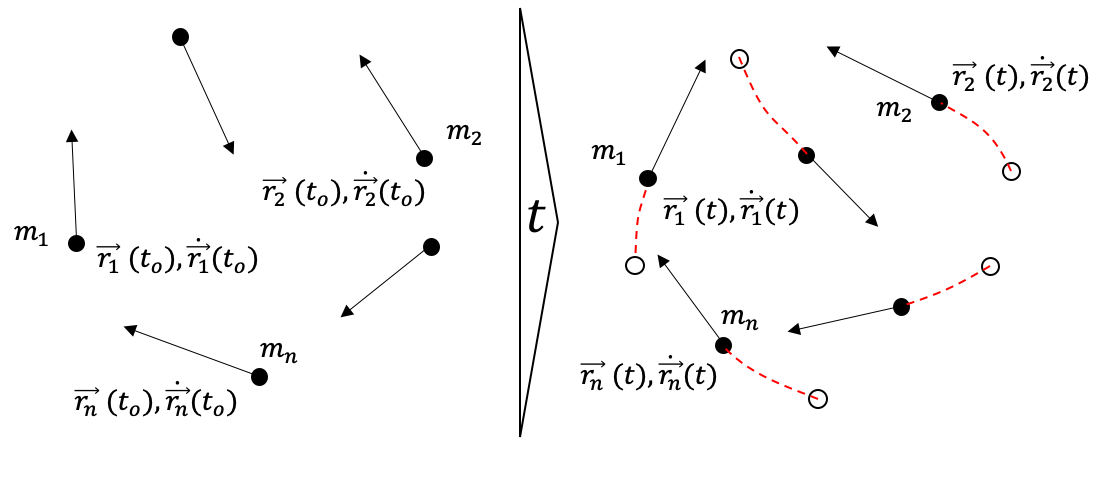
\includegraphics[width=1\textwidth]{./figures/horizontal_ncuerpos_formulacion.png}
\caption{El problema de los N cuerpos: dadas las condiciones iniciales
de un conjunto de N partículas puntuales, predecir la posición y
velocidad de las partículas en cualquier instante
futuro.\label{fig:ncuerpos_formulacion}}
\end{figure}

Esta formulación del problema, que tiene un marcado estilo matemático,
puede matizirse con algunos comentarios físicos:

\begin{itemize}
\tightlist
\item
  Asumimos que en un momento dado del tiempo \(t_0\), las posiciones y
  velocidades de todas las partículas (condiciones iniciales) son
  conocidas \(\{{\vec r_i(t_0)},{\dot{\vec r}_i(t_0)}\}_{N}\) (ver
  \autoref{fig:ncuerpos_formulacion}.) Adicionalmente suponemos que las
  posiciones de dos o más partículas no coinciden completamente en el
  tiempo inicial \(t_0\). El problema de los N cuerpos consiste entonces
  en encontrar las posiciones y velocidades de todas las partículas en
  un instante futuro de tiempo \(t\), es decir encontrar
  \(\{{\vec r_i(t)},{\dot{\vec r}_i(t)}\}_{N}\) .
\end{itemize}

\begin{itemize}
\tightlist
\item
  Al decir que la solución puede, en general, expresarse como una serie
  de una variable dependiente del tiempo (no necesariamente el tiempo
  mismo), el enunciado admité que no es necesario que las posiciones y
  velocidades deban expresarse en la forma de funciones analíticas (p.e.
  polinomios, funciones trigonométricas, función logarítmica o
  exponencial, etc.) Es claro que, al menos para propósitos del cálculo
  aproximado de la solución, tener una serie convergente puede ser tan
  útil como tener una solución analítica (aunque naturalmente no es lo
  mismo, especialmente si la serie converge muy lentamente como veremos
  más adelante.)
\end{itemize}

\begin{itemize}
\tightlist
\item
  La convergencia uniforme es una condición matemática rigurosa,
  aplicada a las sucesiones y series, que implica, en pocas palabras que
  las posiciones y velocidades calculadas con la serie sean tan cercanas
  como se desee a las posiciones y velocidades reales, sin importar el
  tiempo en el que se calculen.
\end{itemize}

\begin{itemize}
\tightlist
\item
  Como lo admite implícitamente el enunciado, no se espera que sea
  posible predecir el estado del sistema en cualquier instante futuro.
  En el caso, por ejemplo, en el que las condiciones iniciales conduzcan
  a una colisión, es decir, una situación en la que al menos dos
  partículas en el sistema podrían situarse a una distancia nula una de
  otra, se produciría una \emph{singularidad} matemática en el sistema
  (fuerzas infinitas). Aún en casos en los que se produzcan colisiones,
  se espera que sea posible predecir la evolución del sistema entre el
  tiempo inicial y el tiempo de la primera colisión.
\end{itemize}

Matemáticamente, el problema de los N cuerpos es equivalente la solución
de las e.d.m. de todas las partículas (Ecs. \ref{eq:edm_sistema}):

\[
\left\{\ddot{\vec r}_i=\frac{1}{m_i}\sum_{j\neq i} \vec F_{ij}\right\}_{N},
\] donde no sobra recordar que según las convenciones usadas aquí,
\(\vec F_{ij}\) es la fuerza ejercida \emph{sobre} la partícula \(i\)
\emph{por} la partícula \(j\).

Como esta implícito aquí, asumiremos que no existe ninguna fuerza
externas sobre las partículas del sistema, p.e. fricción con un medio,
interacción con un campo externo, etc.

De acuerdo a la formulación del problema presentada en la Definición
\ref{box:def:problema.n.cuerpos}, asumimos que la dinámica es
estrictamente newtoniana, lo que incluye suponer que la única
interacción a distancia entre las partículas es la interacción
gravitacional newtoniana (ver Pos. \ref{pos:gravitacion.universal}, Ec.
\ref{eq:fuerza_gravitacional}):

\[
\vec{F}_{ij} = -\frac{Gm_i m_j}{r_{ij}^3} \vec r_{ij}.
\] donde tampoco sobra recordar que en lo sucesivo el vector relativo
\(\vec{r}_{ij}\equiv\vec{r}_i - \vec{r}_j\) apunta en la dirección que
va de la partícula que produce la fuerza (partícula \(j\)) hacia la
partícula que la experimenta (partícula \(i\)).

En términos explícitos, finalemente, el problema de los N cuerpos en
mecánica celeste, consiste en resolver el conjunto de ecuaciones
diferenciales:

\begin{equation}
\label{eq:ncuerpos_formulacion_ecuaciones}
\left\{\ddot{\vec r}_i= -\sum_{j\neq i} \frac{\mu_j}{r_{ij}^3} \vec{r}_{ij} \right\}_{N},
\end{equation}

donde hemos introducido el \textbf{parámetro gravitacional}
\(\mu_j\equiv G m_j\) sobre el que volveremos en la
\autoref{ncuerpos_solucion_numerica}.
\begin{box_history}{Un poco de historia}{}{nofloat}
\small

\textbf{Henri Poincaré y el premio del Rey Oscar.} En 1889, el
matemático sueco Mittag-Leffer convenció al rey Oscar II de Suecia de
que, con motivo de la celebración de su cumpleaños presentará al mundo
un nuevo concurso matemático.

Entre los problemas formulados en el concurso del rey Oscar II se
encontraba, precisamente, el problema de los N cuerpos. La formulación
del problema presentada en este capítulo, es literalmente la que preparó
para el Rey, el matemático alemán Karl Weierstrass
(``\hreffoot{https://es.forvo.com/search/Weierstrass/de/}{Vierstrass}''),
inspirado originalmente por las ideas del también matemático alemán
Peter Gustav Dirichlet (``Diriclet'').

Uno de los participantes del concurso, fue el matemático Francés
\textbf{Henri Poincaré}
(``\hreffoot{https://es.forvo.com/search/Henri\%20Poincare/}{Honri
Poancaré}'') , que contaba para la época con 35 años (ver
\autoref{fig:henri_poincare}).

Poincaré nació en Francia el 29 de abril de 1854 y se graduo como doctor
en matemáticas en 1879 bajo la orientación de Charles Hermite
(``\hreffoot{https://es.forvo.com/search/Charles\%20Hermite/fr/}{Charle
ermit}'').

Las mayores contribuciones de Poincaré, como matemático, se produjeron
en la teoría de ecuaciones diferenciales. Sin embargo, por sus estudios
posteriores de ingeniería, su posición como profesor de la Universidad
de Paris (La Sorbona) en las áreas de Mecánica, Física Matemática,
Teoría de la Probabilidad, Mecánica Celeste y Astronomía, además del
reconocimiento público que lo llevo a ser miembro de la Oficina de
Longitudes de Francia en 1897 y elegido presidente de la Academia
Francesa de Ciencias en 1906, los conocimientos de Poincaré se
extendieron a muchas otras disciplinas. De allí que sea considerado un
\textbf{Polímata} o un ``hombre universal'' (alguien que domina muchas
disciplinas intelectuales o artísticas) un apelativo que comparte con
personajes como Aristóteles o Leonardo da Vinci).

El artículo presentado por Poincaré en el concurso del Rey Oscar II,
titulado ``Sobre el problema de los tres cuerpos y las ecuaciones de la
dinámica''\cite{Poincare1890}, fue declarado, sin lugar a dudas el
ganador del concurso. Pero mo sin alguna polémica. De un lado el trabajo
no resolvía el porblema general y del otro contenía algunos errores que
fueron solo corregidos después. Adicionalmente la ``solución'' cuya
existencia demostraba Poincaré suponía que los cuerpos se mantendrían
siempre a una distancia mayor a un cierto valor mínimo. El mismo
Poincaré admitiría, que la solución general al problema tal vez no se
encontraría pronto y que serían necesarias ``herramientas analíticas
infinitamente más complicadas que las disponibles en la época.'' Aún así
los métodos introducidos por Poincaré en aquel trabajo de 1890,
influenciarían de forma importante la mecánica celeste y serían la base
para el desarrollo de la teoría del caos.

El problema de los tres cuerpos, formulado a la manera del concurso del
rey Oscar II, fue finalmente resuelto en 1912 por el matemático
Finlandés Karl Sundman \cite{Sundman1913ThreeBody}. En este trabajo
Sundman probó la existencia de series que describían la posición de los
tres cuerpos y que convergían para tiempos arbitrarios. Una excelente
síntesis histórica de la contribución (poco apreciada) de Sundman puede
encontrarse en \cite{Barrow2010Sundman}.

\end{box_history}
\begin{figure}[ht!]
\centering
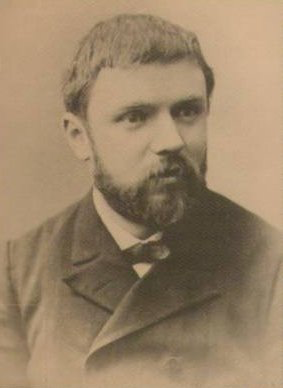
\includegraphics[width=0.5\textwidth]{./figures/vertical_henri_poincare.png}
\caption{Fotografía de Henri Poincaré hacia el año 1886, unos años antes
de realizar su trabajo histórico sobre el problema de los tres cuerpos
(Foto: Eugène Pirou)\label{fig:henri_poincare}}
\end{figure}



\hypertarget{solucion_analitica}{%
\section{¿Solución analítica?}\label{solucion_analitica}}

Como aprendimos en la \autoref{integracion_edm}, una manera posible
para buscar una solución analítica a las \(6N\) ecuaciones diferenciales
del problema de los N cuerpos (Ec.
\ref{eq:ncuerpos_formulacion_ecuaciones}), o para al menos, aprender
cosas sobre la dinámicas del sistema aunque no obtengamos la solución,
es la de buscar tantas constantes de movimiento (cuadraturas) como sea
posible.

Como habíamos visto, para convertir el problema diferencial en uno
algebraico completamente determinado (igual numero de ecuaciones que de
incognitas), es necesario encontrar \(6N\) cuadraturas, es decir, un
número de constantes de movimiento igual al de variables del sistema.

En esta sección usaremos los resultados generales sobre la dinámica de
sistemas de partículas que obtuvimos en la
\autoref{sistemas_particulas} además de los métodos matemáticos
introducidos en la \autoref{integracion_edm}, para encontrar las
primeras integrales de movimiento del problema de los N cuerpos y
acercarnos así a su solución analítica.



\hypertarget{ncuerpos_teoremas_conservacion}{%
\subsection{Aplicación de los teoremas de
conservación}\label{ncuerpos_teoremas_conservacion}}

En la forma específica del problema de los N cuerpos presentada aquí,
asumimos que el sistema de partículas esta aislado del Universo, es
decir, sobre los cuerpos no actúa ninguna fuerzas externa.

Como vimos en la \autoref{teoremas_conservacion}, esta condición
implica que tanto el momentum lineal total del sistema (ver Teo.
\ref{box:teo:conservacion.p.sistemas}), como su momentum angular total
(ver Teo. \ref{box:teo:conservacion.L.sistemas}) se conservan.

De acuerdo con esto, las funciones:

\[
\begin{array}{rcl}
\sum m_i \dot{\vec r}_i & = & \vec P_\mathrm{CM}\\
\sum m_i {\vec r}_i\times\dot{\vec r}_i & = & {\vec L}
\end{array}
\] son las primeras constantes de movimiento que reconocemos para el
problema.

Dada la importancia que el método de cuadraturas tiene en el desarrollo
de muchos de los resultados en este libro, en las siguientes secciones
confirmaremos este resultado, lo interpretaremos en el contexto del
problema de los N cuerpos y en particular estudiaremos su implicación
para algunos sistemas astronómicos de interés, pero más importante,
encontraremos dos constantes adicionales que no habíamos deducido hasta
ahora en el caso general de sistemas de muchas partículas.

\hypertarget{ncuerpos_momento}{%
\subsection{Momento lineal}\label{ncuerpos_momento}}

Como vimos en la \autoref{fuerzas_centro_masa}, la manera de probar
la conservación del momento angular en el problema de los N cuerpos,
consiste en sumar las e.d.m. de cada una de las partículas (Ecs.
\ref{eq:ncuerpos_formulacion_ecuaciones}):

\begin{equation}
\label{eq:ncuerpos_suma_edm}
\sum_i m_i\ddot{\vec r}_i = -\sum_i \sum_j \frac{m_i \mu_j}{r_{ij}^3} \vec{r}_{ij}
\end{equation}

En el lado derecho de esta ecuación, el término en el denominador es
simétrico, \(r_{ji}=r_{ij}\), mientras el término en el numerador,
\(\vec{r}_{ji}=\vec{r}_i-\vec{r}_j\) es \emph{antisimétrico} (el signo
cambia al cambiar el orden de los índices). Como resultado, por cada
término en la doble sumatoria (por ejemplo el término \(i=1\), \(j=4\))
habra un término idéntico pero de signo contrario (el término con
\(i=4\), \(j=1\)) que lo anulará. Físicamente, esta propiedad matemática
es equivalente a aplicar postulado de acción y reacción que usamos para
deducir la Ec. (\ref{eq:edm_sistema}).

Así, el lado derecho de la Ec. (\ref{eq:ncuerpos_suma_edm}) siempre será
nulo (sin importar el número de partículas) y la suma de las e.d.m.
será:

\begin{equation}
\sum m_i\ddot{\vec r}_i = 0.
\end{equation}

Como era de esperarse esta ecuación es equivalente a la e.d.m. de un
sistema de partículas sobre el que no actúan fuerzas externas (Ec.
\ref{eq:edm_sistema}.)

En forma de cuadraturas la misma ecuación se escribe:

\[
\frac{d}{dt}\left(\sum_i m_i \dot{\vec{r}}_i\right) =0,
\] donde como siempre asumimos que las masas de todas las partículas del
sistema \(\{m_i\}\) son constantes.

Esta expresión no es otra cosa que una forma del teorema de conservación
del momento lineal y provee la primera constante (vectorial) de
movimiento del problema de N cuerpos:

\begin{equation}
\label{eq:ncuerpos_momento}
\sum_i m_i \dot{\vec{r}}_i={\vec P}_\mathrm{CM}
\end{equation}

Por tratarse de una expresión vectorial, en esta cuadratura hay
contenidas en realidad tres constantes de movimiento:
\(\sum_i m_i\dot{x}_i=P_{\mathrm{CM},x}\),
\(\sum_i m_i\dot{y}_i=P_{\mathrm{CM},y}\) y
\(\sum_i m_i\dot{z}_i=P_{\mathrm{CM},z}\).
\begin{box_note}{Nota}

\textbf{El sistema de referencia del centro de masa.} La constancia de
\({\vec P}_{\mathrm{CM}}\) en el problema de los N cuerpos, nos permite
introducir un sistema de referencia inercial ideal para la descripción
simplificada del problema. Naturalemente nos referimos al sistema de
referencia del centro de masa, que tiene, respecto al sistema de
referencia general considerado hasta aquí, una velocidad constante e
igual a \({\vec V}_{\mathrm{CM}}={\vec P}_{\mathrm{CM}}/M\) (donde
\(M=\sum m_i\)).

El movimiento de las partículas en este sistema de referencia es el más
\emph{simple} que podemos percibir desde un sistema de referencia
inercial. Por la misma razón, en lo sucesivo y siempre y cuando no se
diga lo contrario, la dinámica de la mayoría de los sistemas de N
cuerpos considerados en este libro se describirá en el sistema de
referencia de su centro de masa.

\end{box_note}
\hypertarget{ncuerpos_centro_masa}{%
\subsection{Posición del centro de masa}\label{ncuerpos_centro_masa}}

Una segunda constante de movimiento puede obtenerse aplicando
cuadraturas a la primera integral (Ec. \ref{eq:ncuerpos_momentum}):

\[
\frac{\mathrm{d}}{\mathrm{d}t}\left(\sum_i m_i \vec{r}_i\right)=\frac{\mathrm{d}}{\mathrm{d}t}\left({\vec P}_\mathrm{CM} t\right)
\]

De donde podemos escribir:

\begin{equation}
\label{eq:ncuerpos_centro_masa}
\sum_i m_i \vec{r}_i-{\vec P}_\mathrm{CM} t=M\vec R_0
\end{equation}

Para expresar está última constante de movimiento, hemos elegido,
arbitrariamente, llamar a su valor como \(M\vec R_0\), donde \(M\) es la
masa total del sistema (que también es un valor constante). La elección
de esta parametrización para el valor de la integral, no modifica en
nada el hecho que el lado derecho de la Ec.
(\ref{eq:ncuerpos_centro_masa}) es constante también.

¿Cómo podemos interpretar físicamente la constante de movimiento en la
Ec. (\ref{eq:ncuerpos_centro_masa})? Si dividimos la expresión de esta
constante por la masa total del sistema \(M\) y la escribimos como:

\[
\frac{\sum_i m_i \vec{r}_i}{M}=\vec R_0+\vec V t,
\] podemos identificar, del lado izquierdo, la posición del centro de
masa del sistema en cualquier tiempo
\({\vec R}_{\rm CM}=\sum m_i\vec{r}_i/M\) (ver Ec.
\ref{eq:centro_masa}). Del lado derecho, por otro lado, encontramos a
\({\vec V}_\mathrm{CM} t\), que no es otra cosa que el desplazamiento
que sufre el centro de masa al moverse con velocidad constante
\({\vec V}_\mathrm{CM}={\vec P}_\mathrm{CM}/M\). En consecuencia podemos
entonces concluir que \(\vec R_0\) no es otra cosa es la posición
inicial del centro de masa. Así, la Ec. (\ref{eq:ncuerpos_centro_masa})
es la constante de movimiento asociada al centro de masa.

De nuevo, por tratarse de una expresión vectorial, la Ec.
(\ref{eq:ncuerpos_centro_masa}) corresponde en realidad a tres
constantes en lugar de una:
\(\sum_i m_i x_i-P_{\mathrm{CM},x} t=M x_{\mathrm{CM},0}\),
\(\sum_i m_i y_i-P_{\mathrm{CM},y} t=M y_{\mathrm{CM},0}\) y
\(\sum_i m_i z_i-P_{\mathrm{CM},z} t=M z_{\mathrm{CM},0}\).

En el sistema de referencia del centro de masa que habíamos mencionado
en una nota anterior, esta constante de movimiento se puede escribir de
forma simplificada como:

\begin{equation}
\label{eq:ncuerpos_centro_masa}
\sum_i m_i {{\vec r}_i}'=\vec 0,
\end{equation} donde, como hicimos en la
\autoref{dinamica_centro_masa}, las cantidades primadas son medidas
respecto al centro de masa.

Esta expresión confirma la intuición expresada antes de que en este
sistema de referenia la descripción del problema es la más simple
posible.

\hypertarget{ncuerpos_momento_angular}{%
\subsection{Momentum angular}\label{ncuerpos_momento_angular}}

Como hicimos en la \autoref{teoremas_conservacion}, si tomamos las
e.d.m. del sistema de partículas (Ec.
\ref{eq:ncuerpos_formulacion_ecuaciones}) y \emph{premultiplicamos}
vectorialmente por el vector posición y la masa de cada partícula (este
será el factor integrante), el resultado es el conjunto de ecuaciones:

\[
\left\{m_i\vec{r}_i\times \ddot{\vec{r}}_i= -m_i\sum_j \frac{\mu_j}{r_{ij}^3} \vec{r}_i\times \vec{r}_{ij} \right\}
\]

Por las propiedades del producto vectorial, el último término en el lado
derecho será,
\(\vec{r}_i\times \vec{r}_{ij}=-\vec{r}_i\times \vec{r}_j\), que es
también antisimétrico. En consecuencia, si sumamos todas las ecuaciones
diferenciales resultantes, obtendremos la ecuación:

\[
\displaystyle \sum_i m_i\vec{r}_i \times \ddot{\vec{r}}_i = \vec{0},
\] que podemos expresar en cuadraturas como:

\[
\frac{d}{dt}\left(\sum_i m_i \vec{r}_i \times \dot{\vec{r}}_i\right) = \vec 0
\]

Esta última ecuación permite identificar la constante de movimiento:

\begin{equation}
\label{eq:ncuerpos_momento_angular}
\sum m_i \vec{r}_i \times \dot{\vec{r}}_i= \vec L
\end{equation} que reconocemos, naturalmente, con el momento angular
total del sistema.

Existe una interesante interpretación geométrica de esta constante de
movimiento: si nos ubicamos en el sistema de referencia del centro de
masa del sistema, la dirección (constante) del vector momento angular
total define un plano invariable (en dirección perpendicular a él). No
importa la posición de las partículas, ni el tiempo en el que se
registren, dicho plano mantendrá siempre su orientación en el espacio. A
este plano se lo conoce históricamente como el \textbf{plano invariable
de Laplace} \cite{Laplace1835Obras}.
\begin{box_definition}{Definición}{box:def:plano.invariable}

\textbf{Plano invariable (de Laplace) y sistema natural de referencia}.
Dado un sistema de N partículas puntuales \(\{m_i\}\), llamamos
\textbf{plano invariable (de Laplace)..} a aquel que tiene como vector
normal \(\hat n={\vec L}'/L'\), donde:

\[{\vec L}'=\sum m_i {{\vec r}_i}' \times {\dot{\vec{r}}_i}'\]

es el momento angular total de las partículas referidas al sistema de
referencia del centro de masa. Dado que \({\vec L}'\) es constante, es
posible usar las posiciones y velocidades de las partículas en un tiempo
arbitrario para calcular la dirección del plano invariable.

Llamamos \textbf{sistema natural de coordenadas} de un sistema de N
cuerpos a aquel que tiene: 1) origen en el centro de masa y 2) plano
\(x-y\) sobre el plano invariable de Laplace (ver Figura
\autoref{fig:plano_invariable}).)

\end{box_definition}
\begin{figure}[t!]
\centering
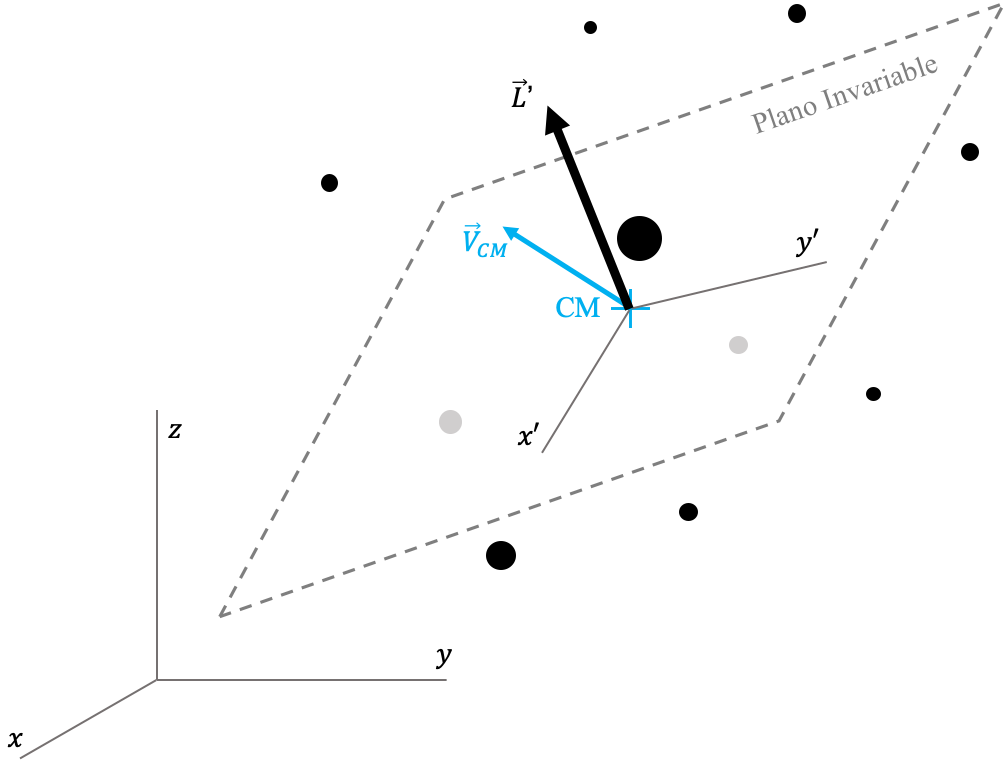
\includegraphics[width=0.7\textwidth]{./figures/square_plano_invariable.png}
\caption{Ilustración gráfica de la orientación del plano invariable de
Laplace. El plano invariable esta definido en el sistema de referencia
inercial del centro de masa y se mueve con él con velocidad
\(V_\mathrm{CM}\) y tiene una orientación dada por el momento angular
total \({\vec L}'\) de las partículas respecto del centro de
masa.\label{fig:plano_invariable}}
\end{figure}

Es importante insistir en que el vector que define la dirección del
plano invariable de Laplace, no es, en general el vector en la Ec.
(\ref{eq:ncuerpos_momento_angular}) que, como vimos en la
\autoref{dinamica_centro_masa} se puede escribir como:

\[
\vec L=M{\vec R}_\mathrm{CM}\times{\vec V}_\mathrm{CM}+\sum m_i {{\vec r}_i}' \times {\dot{\vec{r}}_i}'.
\]

El vector de la Definición \ref{box:def:plano.invariable}, que es
esencialmente el segundo término de la ecuación anterior, no tiene la
misma dirección de \(\vec L\) debido al término
\(M{\vec R}_\mathrm{CM}\times{\vec V}_\mathrm{CM}\) (momento angular del
centro de masa.) Por lo tanto, es muy importante al construir el sistema
de coordenadas natural, tener cuidado de asegurárse que las posiciones y
velocidades de las partículas estén referidas al centro de masa.
\begin{box_history}{Un poco de historia}{}{nofloat}
\small

\textbf{El plano invariable del Sistema Solar.} Durante más de 100 años,
los astrónomos han intentado encontrar la orientación del plano
invariable del Sistema Solar. El esfuerzo no ha sido sencillo, en tanto
durante en el mismo lapso, la masa de los cuerpos no siempre se ha
conocido con precisión e incluso, cuerpos enteramente nuevos se
descubren de vez en cuando.

La determinación más precisa de la orientación del plano invariable se
hizo recientemente \cite{Souami2012SolarPlane} y concluyó que este
importante plano tiene una inclinación, respecto al plano del ecuador en
el sistema ICRF (ver la \autoref{sistemas_referencia_astronomicos})
de 23\(^\circ\) 0' 31``.9 y una longitude del nodo ascendente de
3\(^\circ\) 51' 9''.4 (para una definición de estos ángulos ver la
\autoref{conicas_espacio}.) Esto implica, que el plano invariable
del Sistema Solar esta inclinado respecto al plano de la eclípica de
J2000.0 (que es muy importante en la mecánica celeste al usarse como el
plano de referencia fundamental para el cálculo de posiciones
planetarias) en un ángulo de 1\(^\circ\) 34' 43".3.

\end{box_history}
Usando \texttt{SPICE} podemos hacer una estimación de primer orden de la
inclinación del plano invariable del Sistema Solar, respecto al sistema
de la eclíptica de J2000.0 (ver la
\autoref{sistemas_referencia_astronomicos}.) Para ello podemos
asumir, por simplicidad, que el momentum angular total del sistema esta
concentrado en el Sol y el planeta más masivo, Júpiter (entre los dos
cuerpos concentran el 99.96\% de la masa del sistema.)

Para conseguirlo, primero debemos obtener de los \texttt{kernels} de
\texttt{SPICE}, la masa, posición y velocidad de los cuerpos implicados
en un \emph{tiempo de efemérides} arbitrario (tomaremos
\(t_\mathrm{ef}=0\) por comodidad):

    \begin{code}{Algoritmo}{code:masas_estado_planetas}\begin{Verbatim}[fontsize=\small,commandchars=\\\{\}]
\PY{k+kn}{import} \PY{n+nn}{spiceypy} \PY{k}{as} \PY{n+nn}{spy}

\PY{c+c1}{\PYZsh{}Asumimos un tiempo cualquiera, en este caso t=J2000.0}
\PY{n}{tef}\PY{o}{=}\PY{l+m+mi}{0}

\PY{c+c1}{\PYZsh{}Carga kernels con posiciones (bsp) y masas (tpc)}
\PY{n}{spy}\PY{o}{.}\PY{n}{furnsh}\PY{p}{(}\PY{l+s+s1}{\PYZsq{}}\PY{l+s+s1}{pymcel/data/de430.bsp}\PY{l+s+s1}{\PYZsq{}}\PY{p}{)}
\PY{n}{spy}\PY{o}{.}\PY{n}{furnsh}\PY{p}{(}\PY{l+s+s1}{\PYZsq{}}\PY{l+s+s1}{pymcel/data/de430.tpc}\PY{l+s+s1}{\PYZsq{}}\PY{p}{)}

\PY{c+c1}{\PYZsh{}Parámetro gravitacional, posiciones y velocidades de los cuerpos}
\PY{n}{musol}\PY{o}{=}\PY{n}{spy}\PY{o}{.}\PY{n}{bodvrd}\PY{p}{(}\PY{l+s+s2}{\PYZdq{}}\PY{l+s+s2}{SUN}\PY{l+s+s2}{\PYZdq{}}\PY{p}{,}\PY{l+s+s2}{\PYZdq{}}\PY{l+s+s2}{GM}\PY{l+s+s2}{\PYZdq{}}\PY{p}{,}\PY{l+m+mi}{1}\PY{p}{)}\PY{p}{[}\PY{l+m+mi}{1}\PY{p}{]}\PY{p}{[}\PY{l+m+mi}{0}\PY{p}{]}
\PY{n}{sol}\PY{p}{,}\PY{n}{tluz}\PY{o}{=}\PY{n}{spy}\PY{o}{.}\PY{n}{spkezr}\PY{p}{(}\PY{l+s+s2}{\PYZdq{}}\PY{l+s+s2}{SUN}\PY{l+s+s2}{\PYZdq{}}\PY{p}{,}\PY{n}{tef}\PY{p}{,}
                    \PY{l+s+s2}{\PYZdq{}}\PY{l+s+s2}{ECLIPJ2000}\PY{l+s+s2}{\PYZdq{}}\PY{p}{,}\PY{l+s+s2}{\PYZdq{}}\PY{l+s+s2}{None}\PY{l+s+s2}{\PYZdq{}}\PY{p}{,}\PY{l+s+s2}{\PYZdq{}}\PY{l+s+s2}{SSB}\PY{l+s+s2}{\PYZdq{}}\PY{p}{)}
\PY{n}{rsol}\PY{o}{=}\PY{n}{sol}\PY{p}{[}\PY{p}{:}\PY{l+m+mi}{3}\PY{p}{]}
\PY{n}{vsol}\PY{o}{=}\PY{n}{sol}\PY{p}{[}\PY{l+m+mi}{3}\PY{p}{:}\PY{p}{]}
\PY{n}{mujupiter}\PY{o}{=}\PY{n}{spy}\PY{o}{.}\PY{n}{bodvrd}\PY{p}{(}\PY{l+s+s2}{\PYZdq{}}\PY{l+s+s2}{JUPITER\PYZus{}BARYCENTER}\PY{l+s+s2}{\PYZdq{}}\PY{p}{,}\PY{l+s+s2}{\PYZdq{}}\PY{l+s+s2}{GM}\PY{l+s+s2}{\PYZdq{}}\PY{p}{,}\PY{l+m+mi}{1}\PY{p}{)}\PY{p}{[}\PY{l+m+mi}{1}\PY{p}{]}\PY{p}{[}\PY{l+m+mi}{0}\PY{p}{]}
\PY{n}{jupiter}\PY{p}{,}\PY{n}{tluz}\PY{o}{=}\PY{n}{spy}\PY{o}{.}\PY{n}{spkezr}\PY{p}{(}\PY{l+s+s2}{\PYZdq{}}\PY{l+s+s2}{JUPITER\PYZus{}BARYCENTER}\PY{l+s+s2}{\PYZdq{}}\PY{p}{,}\PY{n}{tef}\PY{p}{,}
                        \PY{l+s+s2}{\PYZdq{}}\PY{l+s+s2}{ECLIPJ2000}\PY{l+s+s2}{\PYZdq{}}\PY{p}{,}\PY{l+s+s2}{\PYZdq{}}\PY{l+s+s2}{None}\PY{l+s+s2}{\PYZdq{}}\PY{p}{,}\PY{l+s+s2}{\PYZdq{}}\PY{l+s+s2}{SSB}\PY{l+s+s2}{\PYZdq{}}\PY{p}{)}
\PY{n}{rjupiter}\PY{o}{=}\PY{n}{jupiter}\PY{p}{[}\PY{p}{:}\PY{l+m+mi}{3}\PY{p}{]}
\PY{n}{vjupiter}\PY{o}{=}\PY{n}{jupiter}\PY{p}{[}\PY{l+m+mi}{3}\PY{p}{:}\PY{p}{]}
\end{Verbatim}

%%

\end{code}
\vspace{-1em}

%%hidecode


    \begin{Verbatim}[fontsize=\small,commandchars=\\\{\}]
Sol:
	mu = 132712440041.9394 km\^{}3/s\^{}2
	Posición = [-1067598.50226456  -418234.39327422    30837.61810502] km
	Velocidad = [ 0.00931257 -0.01282475 -0.00016333] km/s
Jupiter:
	mu = 126712764.7999999 km\^{}3/s\^{}2
	Posición = [ 5.97499980e+08  4.39186501e+08 -1.51960586e+07] km
	Velocidad = [-7.90052522 11.14330827  0.13069904] km/s
\end{Verbatim}

Nótese que como señalamos antes nos hemos cuidado de calcular tanto la
posición del Sol como de Júpiter, respecto al centro de masa
(baricentro) del sistema solar (\texttt{SSB} por \emph{Solar System
Barycenter} en \texttt{SPICE}.)

Con esta información, el momento angular total del sistema será:

    \begin{code}{}{}\begin{Verbatim}[fontsize=\small,commandchars=\\\{\}]
\PY{c+c1}{\PYZsh{}Constante de gravitación universal:}
\PY{n}{G}\PY{o}{=}\PY{l+m+mf}{6.67e\PYZhy{}20} \PY{c+c1}{\PYZsh{} km\PYZca{}3 / kg s\PYZca{}2}

\PY{c+c1}{\PYZsh{}Momentum angular total}
\PY{k+kn}{from} \PY{n+nn}{numpy} \PY{k}{import} \PY{n}{cross}
\PY{n}{L}\PY{o}{=}\PY{p}{(}\PY{n}{musol}\PY{o}{/}\PY{n}{G}\PY{p}{)}\PY{o}{*}\PY{n}{cross}\PY{p}{(}\PY{n}{rsol}\PY{p}{,}\PY{n}{vsol}\PY{p}{)}\PY{o}{+}\PY{p}{(}\PY{n}{mujupiter}\PY{o}{/}\PY{n}{G}\PY{p}{)}\PY{o}{*}\PY{n}{cross}\PY{p}{(}\PY{n}{rjupiter}\PY{p}{,}\PY{n}{vjupiter}\PY{p}{)}
\end{Verbatim}

%%

\end{code}
\vspace{-1em}

%%hidecode


    \begin{Verbatim}[fontsize=\small,commandchars=\\\{\}]
L = [4.31661898e+35 7.99455257e+34 1.92754426e+37] kg m\^{}2/s\^{}2
\end{Verbatim}

En el algoritmo anterior, para obtener la masa de cada cuerpo, hemos
divido el valor de los parámetros gravitacionales \(\mu\) por la
constante \(G\) (en las unidades apropiadas.)

Con este resultado, la inclinación estimada del plano invariable del
Sistema Solar, se obtiene, finalmente, calculando el ángulo formado
entre el momento angular total y el eje z (que en \texttt{SPICE} es
perpendicular al plano de la eclíptica de J2000.0), es decir,
\(i=\cos^{-1}(L_z/L)\):

    \begin{code}{}{}\begin{Verbatim}[fontsize=\small,commandchars=\\\{\}]
\PY{k+kn}{from} \PY{n+nn}{numpy} \PY{k}{import} \PY{n}{arccos}
\PY{k+kn}{from} \PY{n+nn}{numpy}\PY{n+nn}{.}\PY{n+nn}{linalg} \PY{k}{import} \PY{n}{norm}

\PY{n}{i}\PY{o}{=}\PY{n}{arccos}\PY{p}{(}\PY{n}{L}\PY{p}{[}\PY{l+m+mi}{2}\PY{p}{]}\PY{o}{/}\PY{n}{norm}\PY{p}{(}\PY{n}{L}\PY{p}{)}\PY{p}{)}
\end{Verbatim}

%%

\end{code}
\vspace{-1em}

%%hidecode


    \begin{Verbatim}[fontsize=\small,commandchars=\\\{\}]
i = 1.3046988768626038 grados
  = 1:18:16
\end{Verbatim}

Aquí hemos usado la notación \texttt{grados:minutos:segundos}, mas
conveniente en el contexto de los algoritmos.

La inclinación obtenida, \(i=1^\circ\;18'\;16''\), difiere de la
calculada con todos los cuerpos del Sistema Solar (ver el recuadro el
\emph{Un poco de historia, el plano invariable del Sistema Solar}) en
casi \(16\) minutos de arco (que corresponde a un error relativo de un
poco más del 17\%.) El lector podría obtener una estimación mejor de
esta inclinación si incluye otros cuerpos en el cálculo (ver sección de
problemas al final de este capítulo.)



\hypertarget{ncuerpos_potencial}{%
\subsection{Energía potencial de N cuerpos}\label{ncuerpos_potencial}}

Una manera alternativa de escribir la ecuación de movimiento del
problema de los N cuerpos, es reconociendo que cada una las fuerzas
gravitacionales que actúan sobre las partículas \emph{derivan} de un
potencial (son fuerzas conservativas). Así:

\[
\left\{m_i\ddot{\vec r}_i= -\frac{\partial}{\partial\vec{r}_i}\left(\sum_{j\neq i} m_i V_{j}\right)\right\}_{N},
\] donde \(V_j=-\mu_j/r_{ij}\) es el potencial gravitacional de la
partícula \(j\) (ver \ref{eq:potencial_campo_gravitacional}), medido en
la posición de la partícula \(i\), y la \emph{derivada vectorial}
\(\partial/\partial\vec{r}_i\) es, por definición en este libro, una
representación del operador gradiente, \(\vec{\nabla}_i\), calculado con
respecto a las coordenadas de la partícula \(i\) (ver la
\autoref{derivadas}.)

Si introducimos lo que podemos llamar la \emph{energía potencial
gravitacional mutua} \(U_{ij}\equiv m_i V_j\) (ver Ec.
\ref{eq:energia_fuerza_campo_gravitacional}), la ecuación de movimiento
se puede escribir como:

\begin{equation}
\label{eq:ncuerpos_edm_potencial_individual}
\left\{m_i\ddot{\vec r}_i= -\frac{\partial}{\partial\vec{r}_i} \left(\sum_{j\neq i} U_{ij}\right)\right\}_{N},
\end{equation}

Si bien, la función de energía potencia \(\sum_{j\neq i} U_{ij}\), que
aparece en el lado derecho de las Ecs.
(\ref{eq:ncuerpos_edm_potencial_individual}), es unica para cada
partícual del sistema, existe una interesante propiedad del problema de
los N cuerpos (y otros problemas con \emph{fuerzas de interacción
centrales}) que permite calcular las fuerzas en el sistema, como el
gradiente de una única función de energía potencial. Aunque esta
propiedad es presentada como un resultado trivial en casi todos los
libros de mecánica celeste, esta lejos de serlo por lo que
profundizaremos un momento en ella.

Consideremos el caso particular de un sistema de tres cuerpos. En
términos explícitos, las e.d.m. de este sistema (Ecs.
\ref{eq:ncuerpos_formulacion_ecuaciones}) tienen la forma :

\begin{eqnarray}
\nonumber
m_1 \ddot{r}_1 & = & -\frac{m_1\mu_2}{r_{12}^3}\vec{r}_{12}-\frac{m_1\mu_3}{r_{13}^3}\vec{r}_{13}\\
\nonumber
m_2 \ddot{r}_2 & = & -\frac{m_2\mu_1}{r_{21}^3}\vec{r}_{21}-\frac{m_2\mu_3}{r_{23}^3}\vec{r}_{23}\\
\nonumber
m_3 \ddot{r}_3 & = & -\frac{m_3\mu_1}{r_{31}^3}\vec{r}_{31}-\frac{m_3\mu_2}{r_{32}^3}\vec{r}_{32}\\
\end{eqnarray}

Nótese, por ejemplo, que las fuerzas
\(\vec{F}_{12}=-m_1\mu_2 \vec{r}_{12}/r_{12}^3\) y
\(\vec{F}_{21}=-m_2\mu_1 \vec{r}_{21}/r_{21}^3\), en realidad pueden
obtenerse de una sola energía potencial, a saber,
\(U_{12}=-m_1\mu_2/r_{12}\):

\[
\begin{array}{rcl}
\vec{F}_{12} & = & \partial_{\vec r_1}U_{12} \\
\vec{F}_{21} & = & \partial_{\vec r_2}U_{12} \\
\end{array}
\]

La fuerza \(\vec{F}_{12}\) se obtiene de \(U_{12}\) si se deriva esta
cantidad respecto a \(\vec r_1\); por su lado, la fuerza
\(\vec{F}_{21}\) aparece deribando \(U_{12}\) respecto a \(\vec r_2\).
Una situación similar ocurre con los pares de fuerzas \(\vec{F}_{13}\),
\(\vec{F}_{31}\) y \(\vec{F}_{23}\), \(\vec{F}_{32}\).

Es decir, 6 fuerzas diferentes derivan, en realidad, de solo 3 términos
de energía potencial: \(U_{12}\), \(U_{13}\) y \(U_{23}\).
Explícitamente:

\begin{eqnarray}
\nonumber
m_1 \ddot{r}_1 & = & -\frac{\partial U_{12}}{\partial\vec{r}_1}-\frac{\partial U_{13}}{\partial\vec{r}_1}\\
\nonumber
m_2 \ddot{r}_2 & = & -\frac{\partial U_{12}}{\partial\vec{r}_2}-\frac{\partial U_{23}}{\partial\vec{r}_2}\\
\nonumber
m_3 \ddot{r}_3 & = & -\frac{\partial U_{13}}{\partial\vec{r}_3}-\frac{\partial U_{23}}{\partial\vec{r}_3}\\
\end{eqnarray}

Si reconocemos que
\(\partial U_{23}/\partial \vec{r}_1=\partial U_{13}/\partial \vec{r}_2=\partial U_{12}/\partial \vec{r}_3\),
las e.d.m. se pueden escribir de forma más completa como:

\begin{eqnarray}
\nonumber
m_1 \ddot{r}_1 & = & 
-\frac{\partial U_{12}}{\partial\vec{r}_1}-\frac{\partial U_{13}}{\partial\vec{r}_1}-\frac{\partial U_{23}}{\partial\vec{r}_1}\\
\nonumber
m_2 \ddot{r}_2 & = & -\frac{\partial U_{12}}{\partial\vec{r}_2}-\frac{\partial U_{13}}{\partial\vec{r}_2}-\frac{\partial U_{23}}{\partial\vec{r}_2}\\
\nonumber
m_3 \ddot{r}_3 & = & -\frac{\partial U_{12}}{\partial\vec{r}_3}-\frac{\partial U_{13}}{\partial\vec{r}_3}-\frac{\partial U_{23}}{\partial\vec{r}_3}\\
\end{eqnarray}

Allí identificamos, finalmente, una sola función de energía potencial
para todo el sistema:

\begin{equation}
\label{eq:potencial_tres_cuerpos}
U=U_{12}+U_{13}+U_{23},
\end{equation} de la cual puede calcularse la fuerza sobre cualquier
partícula del sistema usando la prescripción general:

\begin{equation}
\label{eq:ncuerpos_edm_potencial}
\left\{m_i\ddot{\vec{r}}_i=-\frac{\partial  U}{\partial\vec{r}_i}\right\}_N
\end{equation}

Esta es la forma más compacta de escribir las ecuaciones de movimiento
del problema de los N cuerpos.

Estudie cuidadosamente las diferencia entre esta forma de las
ecuaciones, que usa una sola función de energía potencial y la menos
económica forma original escrita en las Ecs.
(\ref{eq:ncuerpos_edm_potencial_individual}).
\begin{box_note}{NOTA}

\textbf{Motivación física de la energía potencial de N cuerpos.} La
deducción que hicimos aquí de la energía potencial de tres cuerpos, es
de naturaleza eminentemente matemática. Sin embargo, una vez obtenida,
es posible dar a ella una interpretación que nos permite entender las
razones físicas profundas por las que la energía potencial del sistema
tiene en realidad un número restringido de términos.

Es claro, físicamente, que al cuantificar la energía total de
interacción de un sistema, solo debemos tener en cuenta \emph{una vez}
la contribución que cada pareja de partículas. Así, el sistema de
partículas 1 y 2 contribuyen con \(U_{12}\) a la energía total, es obvio
entonces que sumar a esa energía el término \(U_{21}\) sería redundante
y físicamente incorrecto. Lo mismo pasa con las energías de interacción
\(U_{13}\) que descartan la necesidad de incluir la \(U_{31}\) y la
\(U_{23}\) que una vez sumada hace innecesario agregar la energía
\(U_{32}\).

Este razonamiento, es la razón \emph{física} por la cual la funcuón de
energía potencial en la Ec. (\ref{eq:potencial_tres_cuerpos}) total solo
contiene tres términos (en lugar de 6 como podría intuirse de la forma
de la Ec. \ref{eq:ncuerpos_edm_potencial_individual}).

¿Podría el lector generalizar este resultado a cuatro cuerpos? O más
interesante aún ¿podría ofrecer una fórmula general para el \emph{número
de términos} que tiene la función de energía potencial de un sistema de
N cuerpos? (intente encontrar la respuesta antes de mirar el pie de
nota) \footnote{La respuesta está en la teoría combinatoria: el número
  de términos de la energía potencial es igual al número de
  combinaciones \(C_{N,k}\) en parejas (\(k=2\)) de N números (las
  partículas del sistema). Es un resultado bien conocido de la
  combinatoria que \(C_{N,k}=N!/[k!(N-k)!]\). Así, por ejemplo, con
  \(N=3\) y \(k=2\), el número de combinaciones es \(C_{3,2}=3!/2!=3\)
  que coincide con el ejemplo desarrollado aquí (ver Ec.
  \ref{eq:potencial_tres_cuerpos}.)}

\end{box_note}
La energía potencial de N cuerpos \(U\), que escribimos en la Ec.
(\ref{eq:potencial_tres_cuerpos}) para un sistema de tres partículas,
puede ahora escribirse, en general, para un sistema de N cuerpos, de dos
maneras diferentes:

\begin{enumerate}
\def\labelenumi{\arabic{enumi}.}
\item
  Restringiendo las sumatorias:

  \begin{equation}
   \label{eq:U_restringido}
   U=-\sum_{i=1}^{i<j}\sum_{j=1}^{j=N} \frac{m_i\mu_j}{r_{ij}}
   \end{equation}

  Una fórmula que se escribe en casi todos los textos y de forma
  simplificada como:

  \[
  U=-\sum_{i<j} \frac{m_i\mu_j}{r_{ij}}
  \]

  Esta expresión es relativamente simple, pero expandir las sumatorias,
  en la práctica, puede ser muy complicado (el lector puede intentar,
  por ejemplo, escribir la energía potencial de un sistema de cuatro
  cuerpos, usando la fórmula anterior y no el razonamiento físico que
  esbozamos en la última \emph{Nota}.)
\item
  Sin restringir las sumatorias:

  \begin{equation}
   \label{eq:U_no_restringido}
   U=-\frac{1}{2}\sum_i\sum_{j\neq i} \frac{m_i\mu_j}{r_{ij}}
   \end{equation}

  El factor \(1/2\) en el lado derecho, aunque extraño desde el punto de
  vista de la física, proviene del hecho de que al no restringir la
  sumatoria sobre la \(i\), apareceran los términos duplicados
  \(m_i\mu_j/r_{ij}\) y \(m_j\mu_i/r_{ji}\) que son exactamente iguales.
\end{enumerate}

En lo que queda de este texto usaremos la parametrización de la Ec.
(\ref{eq:U_no_restringido}).

\hypertarget{ncuerpos_energia}{%
\subsection{Conservación de la energía}\label{ncuerpos_energia}}

Si multiplicamos las Ecs. (\ref{eq:ncuerpos_edm_potencial}) por el
factor integrante \(m_i\vec{r}_i\) (usando el producto punto o producto
escalar) y sumamos sobre todas las partículas (como lo hemos hecho para
obtener las otras constantes de movimiento) obtenemos:

\[
\sum_i m_i \dot{\vec{r}}_i\cdot\ddot{\vec{r}}_i =
-\sum_i\dot{\vec{r}}_i\cdot\frac{\partial  U}{\partial\vec{r}_i}
\]

El lado derecho de esta ecuación corresponde a la regla de la cadena
(ver Ec. \ref{eq:regla_cadena_general}):

\[
\frac{\mathrm{d}U}{\mathrm{d}t}=\frac{\partial U}{\partial \vec{r}_1}\cdot\frac{\mathrm{d}\vec{r}_1}{\mathrm{d}t}+\frac{\partial U}{\partial \vec{r}_2}\cdot\frac{\mathrm{d}\vec{r}_2}{\mathrm{d}t}+\ldots+\frac{\partial U}{\partial \vec{r}_n}\cdot\frac{\mathrm{d}\vec{r}_n}{\mathrm{d}t}
\] lo que permite conseguir el objetivo del factor integrante: escribir
la ecuación diferencial en cuadraturas:

\[
\frac{d}{dt}\left(\frac{1}{2}\sum_i m_i \dot{\vec r_i}^2\right)=-\frac{dU}{dt}
\]

De esta ecuación podemos identificar, finalmente, una nueva constante de
movimiento en el problema de los N cuerpos:

\begin{equation}
\label{eq:ncuerpos_energia}
\frac{1}{2}\sum_i m_i \dot{\vec r_i}^2+U(\{\vec{r}_i\})=E
\end{equation}

Con \(U(\{\vec{r}_i\})=(1/2)\sum_i\sum_{j\neq i} m_i\mu_j/r_{ij}\).

Físicamente el valor de \(E\) corresponde a la energía mecánica total
del sistema de N cuerpos y esta integral no es otra cosa que una
expresión del teorema de convervación de la energúa (ver Teo.
\ref{box:teo:conservacion.energia}) en la ausencia de fuerzas no
conservativas.

\hypertarget{energia_tierra_luna}{%
\subsection{Caso de estudio: el sistema
Tierra-Luna}\label{energia_tierra_luna}}

En un terreno más práctico, sería interesante, usar este resultado, para
preguntarse, por ejemplo, cuánta energía \emph{mecánica} existe en el
sistema Tierra-Luna.

Para ello podemos apoyarnos otra vez de \texttt{SPICE}, como lo hicimos
antes para calcular el momentum angular del sistema Sol-Jupiter (ver
Algoritmo \ref{code:masas_estado_planetas}):

    \begin{code}{Algoritmo}{code:estado_tierra_luna}\begin{Verbatim}[fontsize=\small,commandchars=\\\{\}]
\PY{k+kn}{import} \PY{n+nn}{spiceypy} \PY{k}{as} \PY{n+nn}{spy}

\PY{c+c1}{\PYZsh{}Constante de gravitación universal }
\PY{n}{G}\PY{o}{=}\PY{l+m+mf}{6.67e\PYZhy{}20} \PY{c+c1}{\PYZsh{} km\PYZca{}3 / kg s\PYZca{}2}

\PY{c+c1}{\PYZsh{}Asumimos un tiempo cualquiera, en este caso t=J2000.0}
\PY{n}{tef}\PY{o}{=}\PY{l+m+mi}{0}

\PY{c+c1}{\PYZsh{}Carga kernels con posiciones (bsp) y masas (tpc)}
\PY{n}{spy}\PY{o}{.}\PY{n}{furnsh}\PY{p}{(}\PY{l+s+s1}{\PYZsq{}}\PY{l+s+s1}{pymcel/data/de430.bsp}\PY{l+s+s1}{\PYZsq{}}\PY{p}{)}
\PY{n}{spy}\PY{o}{.}\PY{n}{furnsh}\PY{p}{(}\PY{l+s+s1}{\PYZsq{}}\PY{l+s+s1}{pymcel/data/de430.tpc}\PY{l+s+s1}{\PYZsq{}}\PY{p}{)}

\PY{c+c1}{\PYZsh{}Parámetro gravitacional, posiciones y velocidades}
\PY{n}{mutierra}\PY{o}{=}\PY{n}{spy}\PY{o}{.}\PY{n}{bodvrd}\PY{p}{(}\PY{l+s+s2}{\PYZdq{}}\PY{l+s+s2}{EARTH}\PY{l+s+s2}{\PYZdq{}}\PY{p}{,}\PY{l+s+s2}{\PYZdq{}}\PY{l+s+s2}{GM}\PY{l+s+s2}{\PYZdq{}}\PY{p}{,}\PY{l+m+mi}{1}\PY{p}{)}\PY{p}{[}\PY{l+m+mi}{1}\PY{p}{]}\PY{p}{[}\PY{l+m+mi}{0}\PY{p}{]}
\PY{n}{tierra}\PY{p}{,}\PY{n}{tluz}\PY{o}{=}\PY{n}{spy}\PY{o}{.}\PY{n}{spkezr}\PY{p}{(}\PY{l+s+s2}{\PYZdq{}}\PY{l+s+s2}{EARTH}\PY{l+s+s2}{\PYZdq{}}\PY{p}{,}\PY{n}{tef}\PY{p}{,}
                       \PY{l+s+s2}{\PYZdq{}}\PY{l+s+s2}{ECLIPJ2000}\PY{l+s+s2}{\PYZdq{}}\PY{p}{,}\PY{l+s+s2}{\PYZdq{}}\PY{l+s+s2}{None}\PY{l+s+s2}{\PYZdq{}}\PY{p}{,}\PY{l+s+s2}{\PYZdq{}}\PY{l+s+s2}{EARTH\PYZus{}BARYCENTER}\PY{l+s+s2}{\PYZdq{}}\PY{p}{)}
\PY{n}{rtierra}\PY{o}{=}\PY{n}{tierra}\PY{p}{[}\PY{p}{:}\PY{l+m+mi}{3}\PY{p}{]}
\PY{n}{vtierra}\PY{o}{=}\PY{n}{tierra}\PY{p}{[}\PY{l+m+mi}{3}\PY{p}{:}\PY{p}{]}

\PY{n}{muluna}\PY{o}{=}\PY{n}{spy}\PY{o}{.}\PY{n}{bodvrd}\PY{p}{(}\PY{l+s+s2}{\PYZdq{}}\PY{l+s+s2}{MOON}\PY{l+s+s2}{\PYZdq{}}\PY{p}{,}\PY{l+s+s2}{\PYZdq{}}\PY{l+s+s2}{GM}\PY{l+s+s2}{\PYZdq{}}\PY{p}{,}\PY{l+m+mi}{1}\PY{p}{)}\PY{p}{[}\PY{l+m+mi}{1}\PY{p}{]}\PY{p}{[}\PY{l+m+mi}{0}\PY{p}{]}
\PY{n}{luna}\PY{p}{,}\PY{n}{tluz}\PY{o}{=}\PY{n}{spy}\PY{o}{.}\PY{n}{spkezr}\PY{p}{(}\PY{l+s+s2}{\PYZdq{}}\PY{l+s+s2}{MOON}\PY{l+s+s2}{\PYZdq{}}\PY{p}{,}\PY{n}{tef}\PY{p}{,}
                     \PY{l+s+s2}{\PYZdq{}}\PY{l+s+s2}{ECLIPJ2000}\PY{l+s+s2}{\PYZdq{}}\PY{p}{,}\PY{l+s+s2}{\PYZdq{}}\PY{l+s+s2}{None}\PY{l+s+s2}{\PYZdq{}}\PY{p}{,}\PY{l+s+s2}{\PYZdq{}}\PY{l+s+s2}{EARTH\PYZus{}BARYCENTER}\PY{l+s+s2}{\PYZdq{}}\PY{p}{)}
\PY{n}{rluna}\PY{o}{=}\PY{n}{luna}\PY{p}{[}\PY{p}{:}\PY{l+m+mi}{3}\PY{p}{]}
\PY{n}{vluna}\PY{o}{=}\PY{n}{luna}\PY{p}{[}\PY{l+m+mi}{3}\PY{p}{:}\PY{p}{]}
\end{Verbatim}

%%

\end{code}

Una diferencia importante entre este algoritmo y el que vimos para el
cálculo del momentum angular, es que las posiciones y velocidades de la
Tierra y la Luna, son calculadas respecto a la posición del centro de
masa del sistema (\texttt{EARTH\_BARYCENTER}) en lugar de hacerlo
respecto del baricentro del sistema solar (\texttt{SSB}). Si bien, nada
en la Ec. (\ref{eq:ncuerpos_energia}) nos dice que la energía mecánica
total solo se conserva en el sistema de referencia del centro de masa,
nuestra interpretación del valor de esta cantidad será más fácil allí.
El lector puede intentar hacer el cálculo relativo al baricentro del
sistema solar y comparar con el resultado obtenido aquí.

La energía mecánica total del sistema, será entonces:

    \begin{code}{Algoritmo}{code:energia_tierra_luna}\begin{Verbatim}[fontsize=\small,commandchars=\\\{\}]
\PY{c+c1}{\PYZsh{}Masas}
\PY{n}{mtierra}\PY{o}{=}\PY{n}{mutierra}\PY{o}{/}\PY{n}{G}
\PY{n}{mluna}\PY{o}{=}\PY{n}{muluna}\PY{o}{/}\PY{n}{G}

\PY{c+c1}{\PYZsh{}Energía potencial}
\PY{k+kn}{from} \PY{n+nn}{numpy}\PY{n+nn}{.}\PY{n+nn}{linalg} \PY{k}{import} \PY{n}{norm}
\PY{n}{U}\PY{o}{=}\PY{o}{\PYZhy{}}\PY{n}{G}\PY{o}{*}\PY{n}{mluna}\PY{o}{*}\PY{n}{mtierra}\PY{o}{/}\PY{n}{norm}\PY{p}{(}\PY{n}{rtierra}\PY{o}{\PYZhy{}}\PY{n}{rluna}\PY{p}{)}

\PY{c+c1}{\PYZsh{}Energía cinética}
\PY{n}{K}\PY{o}{=}\PY{l+m+mf}{0.5}\PY{o}{*}\PY{n}{mutierra}\PY{o}{*}\PY{n}{norm}\PY{p}{(}\PY{n}{vtierra}\PY{p}{)}\PY{o}{*}\PY{o}{*}\PY{l+m+mi}{2}\PY{o}{+}\PY{l+m+mf}{0.5}\PY{o}{*}\PY{n}{mluna}\PY{o}{*}\PY{n}{norm}\PY{p}{(}\PY{n}{vluna}\PY{p}{)}\PY{o}{*}\PY{o}{*}\PY{l+m+mi}{2}

\PY{c+c1}{\PYZsh{}Energía mecánica total}
\PY{n}{E}\PY{o}{=}\PY{n}{K}\PY{o}{+}\PY{n}{U}
\end{Verbatim}

%%

\end{code}

    \begin{code}{}{}\begin{Verbatim}[fontsize=\small,commandchars=\\\{\}]
\PY{n+nb}{print}\PY{p}{(}\PY{n}{f}\PY{l+s+s2}{\PYZdq{}}\PY{l+s+s2}{Energía potencial U: }\PY{l+s+si}{\PYZob{}U\PYZcb{}}\PY{l+s+s2}{ kg km\PYZca{}2/s\PYZca{}2}\PY{l+s+s2}{\PYZdq{}}\PY{p}{)}
\PY{n+nb}{print}\PY{p}{(}\PY{n}{f}\PY{l+s+s2}{\PYZdq{}}\PY{l+s+s2}{Energía cinética K: }\PY{l+s+si}{\PYZob{}K\PYZcb{}}\PY{l+s+s2}{ kg km\PYZca{}2/s\PYZca{}2}\PY{l+s+s2}{\PYZdq{}}\PY{p}{)}
\PY{n+nb}{print}\PY{p}{(}\PY{n}{f}\PY{l+s+s2}{\PYZdq{}}\PY{l+s+s2}{Energía mecánica total E: }\PY{l+s+si}{\PYZob{}E\PYZcb{}}\PY{l+s+s2}{ kg km\PYZca{}2/s\PYZca{}2}\PY{l+s+s2}{\PYZdq{}}\PY{p}{)}
\end{Verbatim}

%%

\end{code}

    \begin{Verbatim}[fontsize=\small,commandchars=\\\{\}]
Energía potencial U: -7.369786503549795e+22 kg km\^{}2/s\^{}2
Energía cinética K: 3.4021556025880696e+22 kg km\^{}2/s\^{}2
Energía mecánica total E: -3.967630900961725e+22 kg km\^{}2/s\^{}2
\end{Verbatim}

¿Qué significa que la energía mecánica total del sistema Tierra-Luna sea
negativa?

Como lo comentamos en la \autoref{energia_potencial_gravitacional}
el signo negativo de la energía potencial gravitacional (responsable
aquí del signo negativo de \(E\)) se debe a que escogimos el valor de la
constante \(C\) en la Ec. (\ref{eq:energia_potencial_gravitacional})
como cero.

Siguiendo un razonamiento similar al que usamos en esa sección para
explicar físicamente el significado de esta elección arbitraria (y por
tanto el signo de \(U\)), podemos decir aquí que el valor de \(|E|\) en
el sistema Tierra-Luna y en general en cualquier sistema de dos cuerpos,
es el trabajo \emph{mínimo} requerido para separar a la Tierra y a la
Luna a una distancia inmensa. O, en términos \emph{escatológicos},
\(|E|\) es la energía mínima necesaria para destruir la unión entre
nuestro planeta y su eterna compañera.

No es difícil mostrar (ver problemas al final del capítulo) que esta
energía es igual a la energía cinética de un cuerpo con la masa de la
Luna moviéndose a \$\textasciitilde{}\$1 km/s relativa al centro de masa
del sistema. Es decir, una colisión \emph{elástica} con un cuerpo gemelo
de la Luna podría hacer el trabajo de separarnos de ella\footnote{En la
  vida real la colisión mencionada sería \emph{inelástica}, es decir una
  buena parte de la energía cinética de la se convertiría inicialmente
  en calor y destruiría a la Luna y al impactor}.

Para hacernos ahora a una idea más cercana del valor de esta energía,
las unidades de energía utilizadas aquí, kg km\(^2\)/s\(^2\), que siguen
la convención en \texttt{SPICE} de usar km como unidad de longitud, no
son las más convenientes. Para convertirlas a las unidades del sistema
internacional, los joules, J = kg m\(^2\)/s\(^2\), basta multiplicar las
energía obtenidas anteriormente por un factor de conversión de \(10^6\).

En conclusión podemos decir que (el valor absoluto de) la energía
mecánica total del sistema Tierra-Luna es \(~4\times 10^{28}\) j. Esta
energía es aproximadamente igual a la energía consumida por toda la
humanidad en casi
\hreffoot{https://en.wikipedia.org/wiki/World_energy_consumption}{2 millones
de años}.



\hypertarget{ncuerpos_teorema_bruns}{%
\subsection{Síntesis y teorema de Bruns}\label{ncuerpos_teorema_bruns}}

Hasta aquí hemos identificado las siguientes constantes de movimiento
(cuadraturas) del problema de N cuerpos:

\begin{equation}
\label{eq:ncuerpos_constantes_movimiento}
\begin{array}{rcl}
\sum_i m_i \dot{\vec{r}}_i & = & {\vec P}_\mathrm{CM}\\
\sum_i m_i \vec{r}_i-{\vec P}_\mathrm{CM} t & = & M{\vec R}_\mathrm{CM}\\
\sum m_i \vec{r}_i \times \dot{\vec{r}}_i & = & \vec L\\
\frac{1}{2}\sum_i m_i \dot{\vec r_i}^2+U(\{\vec{r}_i\}) & = & E \\
\end{array}
\end{equation}

Las tres primeras son formas compactas (vectoriales) de expresar, cada
una, tres constantes diferentes, de modo que, en total, tenemos hasta
ahora 10 ecuaciones algebraicas (escalares) que relacionan las 6N
cantidades desconocidas \(\{x_i(t),y_i(t),z_i(t)\}_N\),
\(\{\dot{x}_i(t),\dot{y}_i(t),\dot{z}_i(t)\}_N\).

Es claro que nos falta mucho trabajo por hacer si queremos resolver
incluso el problema más simple (con N=2, necesitaríamos por lo menos 12
cudraturas para resolver el sistema.)

En el año 1887 el destacado matemático Ernst Heinrich Bruns, en un
artículo titulado \emph{Sobre las integrales del problema de varios
cuerpos} \cite{Bruns1887Integrales} demostró que, al menos para el
problema de los tres cuerpos, no existen otras primeras integrales de
movimiento que puedan expresarse en términos de funciones algebráicas de
las posiciones y velocidades de las partículas.

En el año 2000, este resultado fue generalizado a sistemas con un número
arbitrario de partículas y de dimensiones espaciales, constituyéndose en
lo que se conoce hoy como el poderoso \textbf{teorema de Bruns
generalizado} \cite{Julliard2000Bruns}:
\begin{box_theorem}{Proposición}{box:teo:bruns}

\textbf{Teorema de Bruns generalizado.} En el problema newtoniano de
(M+1) cuerpos en \({\rm I\!R}^p\), con \(M\geq 2\) y
\(1\leq p\leq M+1\), toda primera integral que es algebraica respecto a
las posiciones, el momento lineal y el tiempo, es una función algebraica
de las primeras integrales clásicas: la energía, las p(p-1)/2
componentes del momento angular, y las 2p constantes que vienen del
movimiento lineal uniforme del centro de masa.

\end{box_theorem}
En el caso particular que hemos estudiado aquí en el que las partículas
se mueven en tres dimensiones, es decir en \({\rm I\!R}^3\) o bien
\(p=3\), según el teorema generalizado de Bruns, las únicas integrales
de movimiento \emph{independientes} son: (1) la energía, (2,3,4)
\(p(p-1)/2=3(3-1)/2=3\) componentes del momento angular y (5,6,7,8,9 y
10) \(2p=6\) constantes del movimiento lineal uniforme del centro de
masa (3 para el momento lineal y 3 para la posición inicial del centro
de masa.)

Es decir, para problemas de \(N\) cuerpos en 3 dimensiones las 10
cuadraturas escritas en las Ecs.
(\ref{eq:ncuerpos_constantes_movimiento}) son las únicas que podemos
encontrar.

Este resultado parece desesperanzador dado que implica que por mucho que
lo intentemos, no podemos obtener el número de constantes necesarias
para expresar el problema de los N cuerpos como un conjunto completo de
cuadraturas.

Esto, sin embargo, no significa, de un lado, que las cuadraturas
obtenidas no puedan enseñarnos cosas muy interesantes sobre los sistemas
de N cuerpos (como ilustraremos en la siguiente sección y en el
\autoref{problema_tres_cuerpos}.)

Del otro lado, y más importante aún, la limitación impuesta por el
teorema de Bruns, no implica necesariamente que el problema no tenga
solución: el hecho de no encontrar cuadraturas suficientes solo
significa que una solución algebraica es imposible.

En realidad, y contrario a la ``mitología tradicional'', el problema de
los N cuerpos, al menos en el caso de sistemas con momento angular cero,
tiene solución en series, como lo exigía el concurso del Rey Oscar II
(ver el recuadro \emph{Un poco de historia, la solución al problema de
los N cuerpos}.) Dicha solución, que no presentaremos en este libro por
razones del nivel matemático exigido (el lector avanzado puede ir
directamente a la literatura especializada), sin embargo, converge muy
lentamente y se necesitan normalmente millones de términos para
aproximar la posición de las partículas incluso en intervalos de tiempo
extremadamente cortos \cite{Diacu1996Solution}.
\begin{box_history}{Un poco de historia}{}{nofloat}
\small

\textbf{La solución al problema de los N cuerpos.} En el año 1990, casi
exactamente 100 años después de la formulación del problema en el
concurso del Rey Oscar II, el matemático chino Wang Qiu-Dong
\cite{Wang1990GlobalSolution} y, antes de él (posiblemente) el ruso L.
K. Babadzhaniants (\cite{Babadzhaniants1979Continuation},
\cite{Babadzhaniants1993}) demostraron la existencia de una solución al
problema de N cuerpos, con las condiciones expresadas en el problema
original (ver la \autoref{ncuerpos_formulacion}), al menos para el
caso de un sistema con momentum angular total nulo. Con este resultado,
Wang y Babadzhaniants habrían extendido el resultado obtenido en 1912
por Karl Sundman, quién probo la existencia de dicha solución existe en
el caso de N=3, incluso en sistemas con un momento angular no nulo. Esto
es lo más cerca que la ciencia ha estado de resolver analíticamente el
problema de los N cuerpos.

\end{box_history}
\bigskip

El obstáculo que en la solución práctica al problema de los N cuerpos
representan, de un lado el teorema de Bruns y del otro la lenta
convergencia de las series descubiertas en el último siglo para la
solución general al problema, nos llevará, en las siguientes secciones y
en los capítulos que les siguen a desarrollar aproximaciones teóricas al
problema de los N cuerpos. Estas aproximaciones nos permitirán formular
explicaciones del comportamiento de sistemas astronómicos reales o
realizar predicciones precisas requeridas para hacer observaciones
astronómicas o controlar el movimiento de vehículos espaciales.

En pocas palabras, los esfuerzos para vencer los obstáculos matemáticos
y físicos que enfrentamos en la solución al problema de los N cuerpos,
representan la mayor parte de lo que conocemos hoy como mecánica
celeste.



\hypertarget{ncuerpos_virial}{%
\section{Energía y virial}\label{ncuerpos_virial}}

En la \autoref{energia_tierra_luna} le pusimos números a una de las
más importantes constantes de movimiento en el problema de los N
cuerpos: la Energía.

Para hacerlo, calculamos la energía mecánica total del sistema
Tierra-Luna y encontramos, contra toda intuición, que era negativa. La
interpretación física de este resultado indica que \emph{hace falta}
energía para separar a la Tierra y la Luna a una distancia enorme; o
dicho en otros términos, que \emph{el valor negativo de la energía de un
sistema de dos partículas indica que la distancia entre ellas esta
acotada y forman un sistema ligado}.

Este interesante resultado, aunque parece obvio, es evidencia de una
afirmación que hemos repetido a lo largo de este capítulo: las
constantes de movimiento o integrales en el problema de los N cuerpos,
pueden no proveer toda la información necesaria para saber dónde estarán
las cuerpos en el futuro, pero ofrecen pistas \emph{útiles} sobre el
destino del sistema.

¿Podríamos generalizar la interpretación del signo de la energía en el
sistema Tierra-Luna a sistema formados por un número arbitrario de
partículas?

\hypertarget{ncuerpos_momento_inercia}{%
\subsection{Momento de inercia}\label{ncuerpos_momento_inercia}}

Para responder a esta última pregunta deberíamos identificar o definir
primero una cantidad física que nos ayude a evaluar la afirmación
``\emph{las partículas se encuentran a una distancia finita}''.

No es difícil descubrir que el momento de inercia total \(I\) del
sistema puede cumplir esta función. Para una nube de partículas, \(I\)
esta definido como\footnote{La definición del momento de inercia aparece
  originalmente en la mecánica newtoniana al estudiar la cinemática y
  dinámica del movimiento de cuerpos rígidos.}:

\begin{equation}
\label{eq:momento_inercia}
I\equiv \sum_i m_i r_i^2
\end{equation}

En términos de esta cantidad podemos decir que el sistema tenderá a
disgregarse, si para \(t\rightarrow \infty\), también
\(I\rightarrow \infty\). Al contrario, el sistema colapsará totalmente,
si, en algún tiempo finito \(t_\mathrm{c}\), el momento de inercia
\(I\rightarrow 0\) . Un sistema \emph{ligado} (que no se disgrega, ni
colapsa), será aquel que se encuentra entre estos dos extremos.

¿Cómo evoluciona \(I\) con el tiempo?

Podemos saberlo si encontramos sus primeras derivadas respecto al
tiempo:

\[
\dot I=2\sum_i m_i \vec{r}_i\cdot\dot{\vec{r}}_i
\]

Esta primera derivada tiene una propiedad interesante: en una misma
cantidad combina, tanto información sobre la posición de las partículas
como sobre su velocidad.

Si definimos:

\begin{equation}
\label{eq:G}
G\equiv\sum_i m_i\vec{r}_i\cdot\dot{\vec{r}_i}
\end{equation} entonces:

\begin{equation}
\label{eq:I_G}
\dot I=2G
\end{equation}

A la ``luz'' de la función \(G\), es más razonable definir un sistema
ligado como aquel en el que simultáneamente la posición y la velocidad
de las partículas están acotadas. En términos de \(G\):

\begin{equation}
\label{eq:G_acotada}
G_\mathrm{min}\leq G\leq G_\mathrm{max}
\end{equation}

\hypertarget{virial}{%
\subsection{El virial}\label{virial}}

¿Como convertir la condición (\ref{eq:G_acotado}), que define a un
sistema ligado, en una condición sobre la energía del sistema?

No es difícil reconocer que la tasa de cambio de \(G\), \(\dot G\),
incluira términos proporcionales a la energía cinética, que es
justamente lo que buscamos:

\begin{equation}
\label{eq:dotG}
\begin{array}{rcl}
\dot G & = & \sum_i m_i {\dot{\vec{r}}_i}^2 + \sum_i \vec{r}_i\cdot (m_i \ddot{\vec{r}}_i)\\
        & = & 2K - \sum_i \vec{r}_i\cdot{\vec F}_i
\end{array}
\end{equation}

En esta expresión aparece una cantidad nueva:

\[{\cal V}=\sum_i {\vec r}_i\cdot{\vec F}_i,\] que depende de las
fuerzas que experimentan las partículas del sistema instantáneamente.

\({\cal V}\) no tuvo una utilidad reconocida previamente en la mecánica
newtoniana hasta 1870 cuando Rudolf Clausius \cite{Clausius1870Virial}
estudiaba la teoría mecánica de los gases y el calor. Por su relación
con la fuerza, cuya palabra en latín es \emph{vis} (con acusativo
\emph{viris}), Clausius llamo a \(\cal V\) el ``virial'' del
sistema\footnote{En realidad el ``virial'' original de Clausius, por
  razones que de verán en la \autoref{teorema_virial} es
  \(\langle\cal V\rangle/2\), donde \(\langle\cal V\rangle\) es el
  promedio de esta cantidad en un intervalo de tiempo muy largo.}.

\hypertarget{identidad_lagrange_jacobi}{%
\subsection{Identidad de
Lagrange-Jacobi}\label{identidad_lagrange_jacobi}}

En el caso del problema de N partículas que interactúan a través de la
fuerza gravitacional Newtoniana (Ec. \ref{eq:ncuerpos_edm_potencial})
\(\{\vec F_i=\partial_{{\vec r}_i} U\}\), el virial viene dado por

\begin{eqnarray}
{\cal V} =\sum_i {\vec r}_i\cdot{\vec F}_i = - \sum_i \vec{r}_i\cdot\partial_{{\vec r}_i} U
\end{eqnarray}

Es posible demostrar (ver problemas al final del capítulo) que la
\(U(\{\vec{r}_i\})\) definida por la Ec. (\ref{eq:U_no_restringido}) es
una función homogénea con \(k=-1\) (ver Def.
\ref{box:def:funciones.homogéneas}).

Por lo tanto, por el Teo. \ref{box:teo:funciones.homogeneas.eules} el
virial de un sistema de N cuerpos es simplemente igual a su energía
potencial:

\[
{\cal V} = - \sum_i \vec{r}_i\cdot\partial_{{\vec r}_i} U = U
\]

Aplicando este resultado a la Ec. (\ref{eq:dotG}) obtenemos la
denominada \textbf{Identidad de Lagrange-Jacobi}:

\begin{equation}
\label{eq:identidad_lagrange_jacobi}
\begin{array}{ccc}
\dot G & = & 2K+U \\
        & = & 2E-U \\
        & = & K+E \\
\end{array}
\end{equation}

Donde, para la segunda y tercera forma de la identidad, hemos usado el
hecho conocido que \(E=K+U\).

En virtud de la relación expresada por la Ec. (\ref{eq:I_G}), una forma
alternativa de esta identidad, muy común en la literatura pero más
oscura en términos del significado de las cantidades involucradas es:

\[
\ddot I=4K+2U
\]

No podemos perder de vista para donde vamos: nuestro propósito era
estudiar la posible relación existente entre la energía mecánica total
de un sistema y el hecho de que sea un sistema ligado o no.

Para ello, consideremos la última forma de la identidad de
Lagrange-Jacobi,

\[\dot G=K+E.\]

Dado que por definición \(K\geq0\), si la energía mecánica total del
sistema es \(E\geq0\), los valores (constantes) de \(\dot G\) y de
\(\ddot I\) serán siempre positivos. Por lo tanto, ambos, \(G\) e \(I\),
independientemente de sus valores iniciales, crecerán indefinidamente y
el sistema tenderá a disgregarse (no será un sistema ligado)\footnote{Es
  interesante anotar que para que \(I\) crezca indefinidamente, basta
  que al menos una partícula, por ejemplo la partícula \(k\), escape del
  sistema, esto es que \(r_k\rightarrow\infty\) cuando
  \(t\rightarrow\infty\).}

Por otro lado si \(E<0\), los signo de \(\dot G\) e \(\ddot I\),
dependerán de la comparación entre \(K\) y \(|E|\). Sin embargo como el
valor de \(K\) es variable en el tiempo (recordemos que solo \(E\) es
constante), no hay manera de predecir, trivialmente, si el sistema
estará ligado o no.

En otras palabras, \(E<0\) es una condición necesaria (puesto que
\(E\geq0\) implica un sistema no ligado), mas no suficiente para que un
sistema de N cuerpos sea ligado.

\hypertarget{teorema_virial}{%
\subsection{Teorema del virial}\label{teorema_virial}}

Puede que no sepamos cuánto vale la energía cinética de un sistema de N
cuerpos en un momento dado (para evaluar por ejemplo el signo de
\(\dot G\) en la identidad de Lagrange-Jacobi), pero podríamos averiguar
si esta acotada por un valor máximo y si valor es finito.

Una manera de hacerlo es calcular el \emph{promedio asintótico} de
\(K(t)\), que definimos como:

\[
\langle K\rangle=\lim_{T\rightarrow\infty} \frac{1}{T}\int_0^{T} K(t)\;\mathrm{d}t
\]

Un sistema en el que la energía cinética tampoco este acotada, para
algún tiempo \(t\), es decir \(K\rightarrow\infty\), tendrá un valor
promedio de la energía cinética \(\langle K\rangle\rightarrow\infty\) y
posiblemente, en virtud de las identidades de Lagrange-Jacobi no sea
tampoco un sistema acotado.

Ahora bien, por la identidad de Lagrange-Jacobi (Ec.
\{eq:identidad\_lagrange\_jacobi\}):

\[
\langle\dot G\rangle=2\langle\dot K\rangle+\langle\dot U\rangle
\] pero:

\[
\langle \dot G\rangle=\lim_{T\rightarrow\infty} \frac{1}{T}\int_0^{T} \dot G dt=\lim_{T\rightarrow\infty} \left(\frac{G(T)-G(0)}{T}\right)
\] donde usamos el teorema fundamental del cálculo (ver Teo.
\ref{box:teo:fundamental.calculo}.)

Ahora bien si \(G\) esta acotada, es decir si
\(G_\mathrm{min}\leq G(t)\leq G_\mathrm{max}\)

\[
\langle \dot G\rangle=\lim_{T\rightarrow\infty} \left(\frac{G(T)-G(0)}{T}\right)\leq\lim_{T\rightarrow\infty} \left(\frac{G_\mathrm{max}-G_\mathrm{min}}{T}\right)=0
\]

Lo que conduce a uno de los más importantes teoremas de la dinámica de
sistemas de muchas partículas:
\begin{box_theorem}{Proposición}{box:teo:virial}

\textbf{Teorema del virial.} Si en un sistema de N cuerpos se define la
cantidad física \(G\equiv\sum_i m_i\vec{r}_i\cdot\dot{\vec{r}_i}\), la
condición \(G_\mathrm{max}\leq G\leq G_\mathrm{min}\) (\(G\) esta
acotada) es necesaria y suficiente\footnote{La condición de que \(G\)
  este acotada es demasiado restringente. Es posible mostrar, por
  ejemplo, que en el caso de un sistema de dos cuerpos que se mueven
  sobre una parábola, también se cumple el teorema del Virial. Por lo
  tanto, existe una condición mucho más general y satisfactoria para
  formular el teorema que puede encontrarse en
  \cite{Pollard1964Virial,}. Esta condición sin embargo no afecta las
  conclusiones que obtenemos en este libro para sistemas generals} para
que el promedio asintótico de las funciones de energía potencial \(U\) y
energía cinética \(K\), satisfagan:

\begin{equation}
  \label{eq:teorema_virial_UK}
  \langle U\rangle=-2\langle K\rangle
  \end{equation}

o equivalentemente:

\begin{equation}
  \label{eq:teorema_virial_EK}
  E=-\langle K\rangle
  \end{equation}

Donde
\(\langle f\rangle = \lim_{T\rightarrow\infty} (1/T) \int_0^T f(t)\;\mathrm{d}t\)

\end{box_theorem}
Puesto en palabras más llanas, en un sistema de N cuerpos ligado, es
decir aquel en el que las posiciones y velocidades están acotadas, el
negativo del promedio asintótico de la energía cinética es igual a la
energía mecánica total. O bien, como es más común encontrarlo en la
literatura:

\begin{equation}
\label{eq:teorema_virial_canonico}
\langle K\rangle=-\frac{1}{2}\langle U\rangle
\end{equation}

Aunque las consecuencias del teorema del virial son interesantes, sus
aplicaciones prácticas en mecánica celeste, especialmente al estudiar
sistemas de pocas partículas, no son muchas. Sin embargo cuando se
estudian, tanto en astronomía como en física, sistemas con un número
significativo de partículas (\(N\rightarrow \infty\)), las implicaciones
pueden ser muy útiles como veremos en el siguiente caso de estudio.

\hypertarget{caso-de-estudio-el-virial-del-sistema-solar}{%
\subsection{Caso de estudio: el virial del Sistema
Solar}\label{caso-de-estudio-el-virial-del-sistema-solar}}

Podemos comprobar el teorema del virial en el caso del sistema Solar,
tomando los cuerpos más masivos del sistema y en los que asumimos se
concentra la mayor parte de la energía cinética y potencial
gravitacional del sistema: El Sol, Júpiter y Saturno.

Para ello, podemos usar como base los Algs.
(\ref{code:estado_tierra_luna},\ref{code:energia_tierra_luna}), con la
diferencia que ahora debemos calcular las posiciones y velocidades de
los cuerpos no en uno, sino en muchos tiempos (valores que nos serviran
para calcular los promedios.) El siguiente algoritmo prepara la
información básica requerida para nuestro cálculo:

    \begin{code}{}{}\begin{Verbatim}[fontsize=\small,commandchars=\\\{\}]
\PY{c+c1}{\PYZsh{}Constante de gravitación universal }
\PY{n}{G}\PY{o}{=}\PY{l+m+mf}{6.67e\PYZhy{}20} \PY{c+c1}{\PYZsh{} km\PYZca{}3 / kg s\PYZca{}2}

\PY{c+c1}{\PYZsh{}Carga kernels con posiciones (bsp) y masas (tpc)}
\PY{k+kn}{import} \PY{n+nn}{spiceypy} \PY{k}{as} \PY{n+nn}{spy}
\PY{n}{spy}\PY{o}{.}\PY{n}{furnsh}\PY{p}{(}\PY{l+s+s1}{\PYZsq{}}\PY{l+s+s1}{pymcel/data/de430.bsp}\PY{l+s+s1}{\PYZsq{}}\PY{p}{)}
\PY{n}{spy}\PY{o}{.}\PY{n}{furnsh}\PY{p}{(}\PY{l+s+s1}{\PYZsq{}}\PY{l+s+s1}{pymcel/data/de430.tpc}\PY{l+s+s1}{\PYZsq{}}\PY{p}{)}

\PY{c+c1}{\PYZsh{}Número de valores de tiempo}
\PY{n}{Nt}\PY{o}{=}\PY{l+m+mi}{100}

\PY{c+c1}{\PYZsh{}Lista de tiempos en los que calcularemos el virial:}
\PY{c+c1}{\PYZsh{}Tomamos 60 años que es aprox. 2 veces el período de Saturno}
\PY{k+kn}{from} \PY{n+nn}{numpy} \PY{k}{import} \PY{n}{linspace}
\PY{n}{tefs}\PY{o}{=}\PY{n}{linspace}\PY{p}{(}\PY{l+m+mf}{0.0}\PY{p}{,}\PY{l+m+mi}{60}\PY{o}{*}\PY{l+m+mf}{356.25}\PY{o}{*}\PY{l+m+mi}{86400}\PY{p}{,}\PY{n}{Nt}\PY{p}{)}

\PY{c+c1}{\PYZsh{}Masas de los cuerpos}
\PY{n}{msol}\PY{o}{=}\PY{n}{spy}\PY{o}{.}\PY{n}{bodvrd}\PY{p}{(}\PY{l+s+s2}{\PYZdq{}}\PY{l+s+s2}{SUN}\PY{l+s+s2}{\PYZdq{}}\PY{p}{,}\PY{l+s+s2}{\PYZdq{}}\PY{l+s+s2}{GM}\PY{l+s+s2}{\PYZdq{}}\PY{p}{,}\PY{l+m+mi}{1}\PY{p}{)}\PY{p}{[}\PY{l+m+mi}{1}\PY{p}{]}\PY{p}{[}\PY{l+m+mi}{0}\PY{p}{]}\PY{o}{/}\PY{n}{G}
\PY{n}{mjupiter}\PY{o}{=}\PY{n}{spy}\PY{o}{.}\PY{n}{bodvrd}\PY{p}{(}\PY{l+s+s2}{\PYZdq{}}\PY{l+s+s2}{JUPITER\PYZus{}BARYCENTER}\PY{l+s+s2}{\PYZdq{}}\PY{p}{,}\PY{l+s+s2}{\PYZdq{}}\PY{l+s+s2}{GM}\PY{l+s+s2}{\PYZdq{}}\PY{p}{,}\PY{l+m+mi}{1}\PY{p}{)}\PY{p}{[}\PY{l+m+mi}{1}\PY{p}{]}\PY{p}{[}\PY{l+m+mi}{0}\PY{p}{]}\PY{o}{/}\PY{n}{G}
\PY{n}{msaturno}\PY{o}{=}\PY{n}{spy}\PY{o}{.}\PY{n}{bodvrd}\PY{p}{(}\PY{l+s+s2}{\PYZdq{}}\PY{l+s+s2}{SATURN\PYZus{}BARYCENTER}\PY{l+s+s2}{\PYZdq{}}\PY{p}{,}\PY{l+s+s2}{\PYZdq{}}\PY{l+s+s2}{GM}\PY{l+s+s2}{\PYZdq{}}\PY{p}{,}\PY{l+m+mi}{1}\PY{p}{)}\PY{p}{[}\PY{l+m+mi}{1}\PY{p}{]}\PY{p}{[}\PY{l+m+mi}{0}\PY{p}{]}\PY{o}{/}\PY{n}{G}
\end{Verbatim}

%%

\end{code}

Con estos datos en mano podemos calcular ahora la energía cinética del
sistema, la energía potencial (Ec. \ref{eq:potencial_tres_cuerpos}) y la
energía total, para cada valor del tiempo escogido. Una vez calculadas
estas cantidades podemos determinar su valor promedio:

    \begin{code}{}{}\begin{Verbatim}[fontsize=\small,commandchars=\\\{\}]
\PY{k+kn}{from} \PY{n+nn}{numpy}\PY{n+nn}{.}\PY{n+nn}{linalg} \PY{k}{import} \PY{n}{norm}
\PY{n}{Ks}\PY{o}{=}\PY{p}{[}\PY{p}{]}
\PY{n}{Us}\PY{o}{=}\PY{p}{[}\PY{p}{]}
\PY{n}{Es}\PY{o}{=}\PY{p}{[}\PY{p}{]}
\PY{k}{for} \PY{n}{tef} \PY{o+ow}{in} \PY{n}{tefs}\PY{p}{:}
    \PY{c+c1}{\PYZsh{}Posiciones, velocidades, energías cinéticas}
    \PY{n}{sol}\PY{p}{,}\PY{n}{tluz}\PY{o}{=}\PY{n}{spy}\PY{o}{.}\PY{n}{spkezr}\PY{p}{(}\PY{l+s+s2}{\PYZdq{}}\PY{l+s+s2}{SUN}\PY{l+s+s2}{\PYZdq{}}\PY{p}{,}\PY{n}{tef}\PY{p}{,}
                        \PY{l+s+s2}{\PYZdq{}}\PY{l+s+s2}{ECLIPJ2000}\PY{l+s+s2}{\PYZdq{}}\PY{p}{,}\PY{l+s+s2}{\PYZdq{}}\PY{l+s+s2}{None}\PY{l+s+s2}{\PYZdq{}}\PY{p}{,}\PY{l+s+s2}{\PYZdq{}}\PY{l+s+s2}{SSB}\PY{l+s+s2}{\PYZdq{}}\PY{p}{)}
    \PY{n}{rsol}\PY{o}{=}\PY{n}{sol}\PY{p}{[}\PY{p}{:}\PY{l+m+mi}{3}\PY{p}{]}
    \PY{n}{vsol}\PY{o}{=}\PY{n}{sol}\PY{p}{[}\PY{l+m+mi}{3}\PY{p}{:}\PY{p}{]}
    \PY{n}{K\PYZus{}sol}\PY{o}{=}\PY{l+m+mf}{0.5}\PY{o}{*}\PY{n}{msol}\PY{o}{*}\PY{n}{norm}\PY{p}{(}\PY{n}{vsol}\PY{p}{)}\PY{o}{*}\PY{o}{*}\PY{l+m+mi}{2}
    
    \PY{n}{jupiter}\PY{p}{,}\PY{n}{tluz}\PY{o}{=}\PY{n}{spy}\PY{o}{.}\PY{n}{spkezr}\PY{p}{(}\PY{l+s+s2}{\PYZdq{}}\PY{l+s+s2}{JUPITER\PYZus{}BARYCENTER}\PY{l+s+s2}{\PYZdq{}}\PY{p}{,}\PY{n}{tef}\PY{p}{,}
                            \PY{l+s+s2}{\PYZdq{}}\PY{l+s+s2}{ECLIPJ2000}\PY{l+s+s2}{\PYZdq{}}\PY{p}{,}\PY{l+s+s2}{\PYZdq{}}\PY{l+s+s2}{None}\PY{l+s+s2}{\PYZdq{}}\PY{p}{,}\PY{l+s+s2}{\PYZdq{}}\PY{l+s+s2}{SSB}\PY{l+s+s2}{\PYZdq{}}\PY{p}{)}
    \PY{n}{rjupiter}\PY{o}{=}\PY{n}{jupiter}\PY{p}{[}\PY{p}{:}\PY{l+m+mi}{3}\PY{p}{]}
    \PY{n}{vjupiter}\PY{o}{=}\PY{n}{jupiter}\PY{p}{[}\PY{l+m+mi}{3}\PY{p}{:}\PY{p}{]}
    \PY{n}{K\PYZus{}jup}\PY{o}{=}\PY{l+m+mf}{0.5}\PY{o}{*}\PY{n}{mjupiter}\PY{o}{*}\PY{n}{norm}\PY{p}{(}\PY{n}{vjupiter}\PY{p}{)}\PY{o}{*}\PY{o}{*}\PY{l+m+mi}{2}
    
    \PY{n}{saturno}\PY{p}{,}\PY{n}{tluz}\PY{o}{=}\PY{n}{spy}\PY{o}{.}\PY{n}{spkezr}\PY{p}{(}\PY{l+s+s2}{\PYZdq{}}\PY{l+s+s2}{SATURN\PYZus{}BARYCENTER}\PY{l+s+s2}{\PYZdq{}}\PY{p}{,}\PY{n}{tef}\PY{p}{,}
                            \PY{l+s+s2}{\PYZdq{}}\PY{l+s+s2}{ECLIPJ2000}\PY{l+s+s2}{\PYZdq{}}\PY{p}{,}\PY{l+s+s2}{\PYZdq{}}\PY{l+s+s2}{None}\PY{l+s+s2}{\PYZdq{}}\PY{p}{,}\PY{l+s+s2}{\PYZdq{}}\PY{l+s+s2}{SSB}\PY{l+s+s2}{\PYZdq{}}\PY{p}{)}

    \PY{n}{rsaturno}\PY{o}{=}\PY{n}{saturno}\PY{p}{[}\PY{p}{:}\PY{l+m+mi}{3}\PY{p}{]}
    \PY{n}{vsaturno}\PY{o}{=}\PY{n}{saturno}\PY{p}{[}\PY{l+m+mi}{3}\PY{p}{:}\PY{p}{]}
    \PY{n}{K\PYZus{}sat}\PY{o}{=}\PY{l+m+mf}{0.5}\PY{o}{*}\PY{n}{msaturno}\PY{o}{*}\PY{n}{norm}\PY{p}{(}\PY{n}{vsaturno}\PY{p}{)}\PY{o}{*}\PY{o}{*}\PY{l+m+mi}{2}

    \PY{c+c1}{\PYZsh{}Distancias entre los cuerpos}
    \PY{n}{r\PYZus{}jup\PYZus{}sol}\PY{o}{=}\PY{n}{norm}\PY{p}{(}\PY{n}{rjupiter}\PY{o}{\PYZhy{}}\PY{n}{rsol}\PY{p}{)}
    \PY{n}{r\PYZus{}sat\PYZus{}sol}\PY{o}{=}\PY{n}{norm}\PY{p}{(}\PY{n}{rsaturno}\PY{o}{\PYZhy{}}\PY{n}{rsol}\PY{p}{)}
    \PY{n}{r\PYZus{}jup\PYZus{}sat}\PY{o}{=}\PY{n}{norm}\PY{p}{(}\PY{n}{rjupiter}\PY{o}{\PYZhy{}}\PY{n}{rsaturno}\PY{p}{)}
    
    \PY{c+c1}{\PYZsh{}Energia potencial}
    \PY{n}{U\PYZus{}jup\PYZus{}sol}\PY{o}{=}\PY{o}{\PYZhy{}}\PY{n}{G}\PY{o}{*}\PY{n}{mjupiter}\PY{o}{*}\PY{n}{msol}\PY{o}{/}\PY{n}{r\PYZus{}jup\PYZus{}sol}
    \PY{n}{U\PYZus{}sat\PYZus{}sol}\PY{o}{=}\PY{o}{\PYZhy{}}\PY{n}{G}\PY{o}{*}\PY{n}{msaturno}\PY{o}{*}\PY{n}{msol}\PY{o}{/}\PY{n}{r\PYZus{}sat\PYZus{}sol}
    \PY{n}{U\PYZus{}jup\PYZus{}sat}\PY{o}{=}\PY{o}{\PYZhy{}}\PY{n}{G}\PY{o}{*}\PY{n}{mjupiter}\PY{o}{*}\PY{n}{msaturno}\PY{o}{/}\PY{n}{r\PYZus{}jup\PYZus{}sat}

    \PY{c+c1}{\PYZsh{}Energía cinética, potencial y mecánica}
    \PY{n}{Ktot}\PY{o}{=}\PY{n}{K\PYZus{}sol}\PY{o}{+}\PY{n}{K\PYZus{}jup}\PY{o}{+}\PY{n}{K\PYZus{}sat}
    \PY{n}{U}\PY{o}{=}\PY{n}{U\PYZus{}jup\PYZus{}sol}\PY{o}{+}\PY{n}{U\PYZus{}sat\PYZus{}sol}\PY{o}{+}\PY{n}{U\PYZus{}jup\PYZus{}sat}
    \PY{n}{E}\PY{o}{=}\PY{n}{Ktot}\PY{o}{+}\PY{n}{U}
    
    \PY{c+c1}{\PYZsh{}Guarda valores en la lista}
    \PY{n}{Ks}\PY{o}{+}\PY{o}{=}\PY{p}{[}\PY{n}{Ktot}\PY{p}{]}
    \PY{n}{Us}\PY{o}{+}\PY{o}{=}\PY{p}{[}\PY{n+nb}{abs}\PY{p}{(}\PY{n}{U}\PY{p}{)}\PY{p}{]}
    \PY{n}{Es}\PY{o}{+}\PY{o}{=}\PY{p}{[}\PY{n+nb}{abs}\PY{p}{(}\PY{n}{E}\PY{p}{)}\PY{p}{]}
\end{Verbatim}

%%

\end{code}
\vspace{-1em}

%%hidecode


    \begin{Verbatim}[fontsize=\small,commandchars=\\\{\}]
<K> = 1.883839013581885e+29 kg km\^{}2/s\^{}2
<U>/2 = -1.8840677890439464e+29 kg km\^{}2/s\^{}2
E = -1.8842965645060087e+29 kg km\^{}2/s\^{}2
\end{Verbatim}

Como vemos, las tres cantidades coinciden (con un margen de error del
0.1\%) con lo esperado a partir del teorema del Virial.

Podemos también hacer un gráfico de \(K\) (lista \texttt{Ks}), \(|U|\)
(lista \texttt{Us}) y \(|E|\) (lista \texttt{Es}):
%%HIDE%%
    \begin{code}{Algoritmo}{code:virial_sistema_solar}\begin{Verbatim}[fontsize=\small,commandchars=\\\{\}]
\PY{k+kn}{from} \PY{n+nn}{numpy} \PY{k}{import} \PY{n+nb}{max}
\PY{k+kn}{import} \PY{n+nn}{matplotlib}\PY{n+nn}{.}\PY{n+nn}{pyplot} \PY{k}{as} \PY{n+nn}{plt}
\PY{n}{plt}\PY{o}{.}\PY{n}{plot}\PY{p}{(}\PY{n}{tefs}\PY{p}{,}\PY{n}{Ks}\PY{p}{,}\PY{l+s+s1}{\PYZsq{}}\PY{l+s+s1}{k\PYZhy{}}\PY{l+s+s1}{\PYZsq{}}\PY{p}{,}\PY{n}{label}\PY{o}{=}\PY{l+s+s2}{\PYZdq{}}\PY{l+s+s2}{\PYZdl{}K\PYZdl{}}\PY{l+s+s2}{\PYZdq{}}\PY{p}{)}
\PY{n}{plt}\PY{o}{.}\PY{n}{plot}\PY{p}{(}\PY{n}{tefs}\PY{p}{,}\PY{n}{Us}\PY{p}{,}\PY{l+s+s1}{\PYZsq{}}\PY{l+s+s1}{b\PYZhy{}\PYZhy{}}\PY{l+s+s1}{\PYZsq{}}\PY{p}{,}\PY{n}{label}\PY{o}{=}\PY{l+s+s2}{\PYZdq{}}\PY{l+s+s2}{\PYZdl{}|U|\PYZdl{}}\PY{l+s+s2}{\PYZdq{}}\PY{p}{)}
\PY{n}{plt}\PY{o}{.}\PY{n}{plot}\PY{p}{(}\PY{n}{tefs}\PY{p}{,}\PY{n}{Es}\PY{p}{,}\PY{l+s+s1}{\PYZsq{}}\PY{l+s+s1}{r:}\PY{l+s+s1}{\PYZsq{}}\PY{p}{,}\PY{n}{label}\PY{o}{=}\PY{l+s+s2}{\PYZdq{}}\PY{l+s+s2}{\PYZdl{}|E|\PYZdl{}}\PY{l+s+s2}{\PYZdq{}}\PY{p}{)}

\PY{n}{plt}\PY{o}{.}\PY{n}{legend}\PY{p}{(}\PY{p}{)}
\PY{n}{plt}\PY{o}{.}\PY{n}{ylim}\PY{p}{(}\PY{l+m+mi}{0}\PY{p}{,}\PY{n+nb}{max}\PY{p}{(}\PY{n}{Us}\PY{p}{)}\PY{p}{)}\PY{p}{;}
\PY{n}{plt}\PY{o}{.}\PY{n}{xlabel}\PY{p}{(}\PY{l+s+s2}{\PYZdq{}}\PY{l+s+s2}{\PYZdl{}t\PYZus{}}\PY{l+s+si}{\PYZob{}ef\PYZcb{}}\PY{l+s+s2}{\PYZdl{} (segundos)}\PY{l+s+s2}{\PYZdq{}}\PY{p}{)}\PY{p}{;}
\PY{n}{plt}\PY{o}{.}\PY{n}{ylabel}\PY{p}{(}\PY{l+s+s2}{\PYZdq{}}\PY{l+s+s2}{\PYZdl{}K,|U|,|E|\PYZdl{} (Joules)}\PY{l+s+s2}{\PYZdq{}}\PY{p}{)}\PY{p}{;}
\end{Verbatim}

%%

\tcblower
\footnotesize
\em ver Figura \ref{fig:code:virial_sistema_solar}
\end{code}

    \begin{center}

\begin{figure}[ht!]
\centering
    \adjustimage{max size={0.8\linewidth}{0.8\paperheight}}{combined_files/combined_1023_0.png}
\caption{Figura correspondiente al código \ref{code:virial_sistema_solar}.\label{fig:code:virial_sistema_solar}}
\end{figure}

    \end{center}
%{ \hspace*{\fill} \\}
    
Como podemos ver en la \autoref{fig:code:virial_sistema_solar}, los
resultados coinciden otra vez con nuestras expectativas:

\begin{itemize}
\item
  La energía total \(E\) (línea punteada) es constante, confirmando la
  validez del teorema de conservación de la energía mecánica en el
  Sistema Solar.
\item
  El valor promedio de la energía cinética del sistema (promedio de la
  línea continua) es igual al valor absoluto de la energía total, lo que
  confirma el teorema del Virial (Ec. \ref{eq:teorema_virial_EK}).
\item
  El valor absoluto del promedio de la energía potencial del sistema
  (promedio de la línea rayada), es el doble que el promedio de la
  energía cinética, lo que confirma también el teorema del Virial (Ec.
  \ref{eq:teorema_virial_UK}).
\end{itemize}

\hypertarget{masa_cumulos_galaxias}{%
\subsection{Caso de estudio: la masa de cúmulos de
galaxias}\label{masa_cumulos_galaxias}}

\begin{figure}[t]
\centering
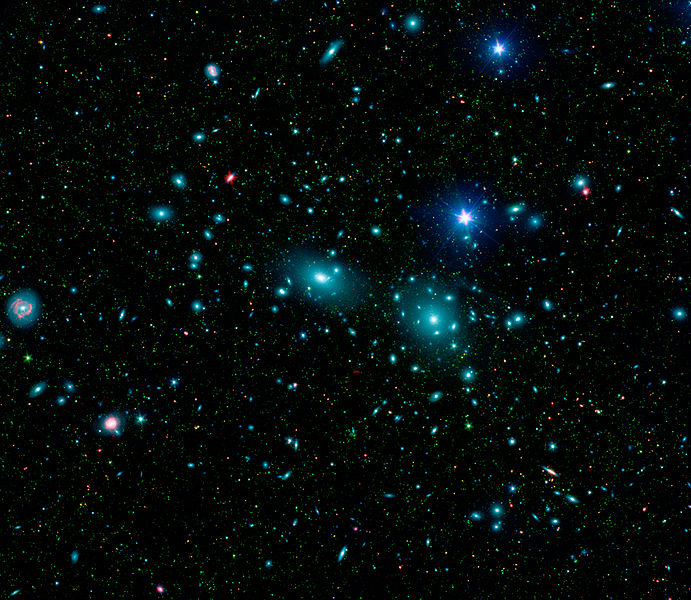
\includegraphics[width=0.7\textwidth]{./figures/square_coma_cluster.png}
\caption{Mosaico en falso color del cúmulo de Galaxias de Coma que
combina imágenes en luz visible e infrarrojo. Crédito: NASA /
JPL-Caltech / L. Jenkins (GSFC).\label{fig:coma_cluster}}
\end{figure}

Otro interesante caso de aplicación del teorema del virial en
astronomía, tiene que ver con el estudio la distribución de masa en
cúmulos de estrellas y galaxias.

Se dice que un cúmulo de galaxias, estrellas o simplemente de
``partículas'' de materia oscura, esta ``virializado'', si ha alcanzado
un estado dinámico en el cuál el teorema del virial describe
apropiadamente los promedios estadísticos de sus propiedades cinemáticas
(velocidades y posiciones.) En virtud de las condiciones del Teo.
(\ref{box:teo:virial}), esto significa, esencialmente, que el sistema es
ligado o estable a largo plazo.

Si asumimos que las partículas del cúmulo tienen una distribución
esférica con una densidad aproximadamente uniforme y con un radio
característico \(R_\mathrm{vir}\) (dentro del cual hay una masa
\(M_\mathrm{vir}\)), la energía potencial promedio del cúmulo será igual
a:

\[
\langle U\rangle=-\frac{3GM_\mathrm{vir}^2}{5R_\mathrm{vir}}
\]

Por su parte si asumimos que todas las partículas tienen la misma masa,
el promedio de la energía cinética total será:

\[
\langle K\rangle=\frac{1}{2} M_\mathrm{vir}\langle v^2\rangle
\]

Usando el teorema del virial obtenemos:

\begin{equation}
\label{eq:virial_v_dispersion}
\frac{3GM_\mathrm{vir}}{5R_\mathrm{vir}}=\langle v^2\rangle
\end{equation}

Si se puede estimar o medir el radio del sistema y el promedio del
cuadrado de las rapideces de las partículas, la masa se puede de un
cúmulo se puede estimar usando:

\[
M_\mathrm{vir}=\frac{5R_\mathrm{vir}\langle v^2\rangle}{3G}
\]

En el algoritmo a continuación estimamos la masa de virial del cúmulo de
Coma (ver \autoref{fig:coma_cluster}) para el cuál se ha estimado que
\(R_\mathrm{vir}\approx 2\times 10^6\) pc (parsecs\footnote{1 parsec =
  3.26 a.l., 1 año-luz = \(9.46\times 10^{12}\) km}) y
\(\langle v^2\rangle^{1/2}\approx 1.000\) km/s (datos obtenidos de
\cite{Gavazzi2009ComaCluster} y \cite{Struble1999ComaCluster}
respectivamente):

    \begin{code}{Algoritmo}{code:masa_coma_cluster}\begin{Verbatim}[fontsize=\small,commandchars=\\\{\}]
\PY{c+c1}{\PYZsh{}Constante gravitacional}
\PY{n}{G}\PY{o}{=}\PY{l+m+mf}{6.67e\PYZhy{}20} \PY{c+c1}{\PYZsh{} km\PYZca{}3 / kg s\PYZca{}2}

\PY{c+c1}{\PYZsh{}Parsec y año\PYZhy{}luz}
\PY{n}{pc}\PY{o}{=}\PY{l+m+mf}{3.26}
\PY{n}{al}\PY{o}{=}\PY{l+m+mf}{9.46e12} \PY{c+c1}{\PYZsh{}km }

\PY{c+c1}{\PYZsh{}Radio del viral}
\PY{n}{Rvir}\PY{o}{=}\PY{l+m+mf}{2e6}\PY{o}{*}\PY{n}{pc}\PY{o}{*}\PY{n}{al}

\PY{c+c1}{\PYZsh{}Dispersión de velocidades}
\PY{n}{v2}\PY{o}{=}\PY{l+m+mi}{1000}\PY{o}{*}\PY{o}{*}\PY{l+m+mi}{2}

\PY{c+c1}{\PYZsh{}Masa del virial del cúmulo}
\PY{n}{Mvir}\PY{o}{=}\PY{l+m+mi}{5}\PY{o}{*}\PY{n}{Rvir}\PY{o}{*}\PY{n}{v2}\PY{o}{/}\PY{p}{(}\PY{l+m+mi}{3}\PY{o}{*}\PY{n}{G}\PY{p}{)}
\end{Verbatim}

%%

\end{code}
\vspace{-1em}

%%hidecode


    \begin{Verbatim}[fontsize=\small,commandchars=\\\{\}]
Masa del virial del cúmulo de Coma:
1.5412093953023487e+45 kg
\end{Verbatim}

Que equivale a \(\sim7\times10^{14}\;M_\odot\)
(\(1\;M_\odot\approx 2\times10^{30}\) kg), o lo que es lo mismo a la
masa de las estrellas y el gas de unas 10.000 galaxias típicas.
\begin{box_history}{Un poco de historia}{}{nofloat}
\small

\textbf{Fritz Zwicky, el teorema del virial y la materia oscura.} La
estimación de la masa del cúmulo de Coma, usando el teorema del virial,
que presentamos aquí, reproduce el trabajo del reconocido astrónomo
suizo Fritz Zwicky
(\hreffoot{https://es.forvo.com/search/Fritz\%20Zwicky/en/}{``Fritz
tsviky''}), uno de los primeros en aplicar el teorema en Astronomía.

En 1933, Zwicky presento en la revista Suiza \emph{Helvetica Physica
Acta} un artículo titulado ``\emph{El desplazamiento al rojo de las
nebulosas extragalácticas}''. En este artículo, usando estimaciones del
número y la masa de las galaxias del Cúmulo (que midió a partir de su
luminosidad), así como medidas de su radio aproximado, Zwicky calculó la
dispersión de velocidades \(\langle v^2\rangle\) con la Ec.
(\ref{eq:virial_v_dispersion}).

Para su sorpresa las velocidades típicas estimadas con el teorema del
virial para las galaxias en el cúmulo,
\(\langle v^2\rangle^{1/2}\approx 80\) km/s, eran casi 10 veces menores
que las que se obtenían al medir el corrimiento espectral de la luz de
las galaxias. Es decir, las galaxias reales se estaban moviendo tan
rápido en el cúmulo que este sistema no podría estar ligado (satisfacer
el teorema del virial).

Otra posibilidad era que la masa usada en la Ec.
(\ref{eq:virial_v_dispersion}) y que el supuso podía estimar a partir de
la materia luminosa de las galaxias, fuera en realidad 10 veces mayor.
Esto implicaba la existencia de una forma de materia invisible (que no
emite luz) y que Zwicky llamo en su artículo en alemán \emph{dunkle
Materie} o Materia oscura.

En 1937, Zwicky publicó, en inglés, una versión extendida de su trabajo
en la prestigiosa revista americana \emph{The Astrophysical Journal}
(\cite{Zwicky1937Clusters}), donde estimó la masa del cúmulo, a partir
de la dispersión de velocidades medida, siguiendo un procedimiento
similar al desarrollado aquí. El resultado confirmo sus estimaciones de
1933: el cúmulo de Coma, que contiene unas \(\sim 1000\) galaxias, tiene
una masa equivalente a \(\sim 10000\) galaxias (tal y como estimamos en
el Algoritmo \ref{code:masa_coma_cluser}.) Es decir el contenido de
materia oscura del cúmulo, supera por un factor de \(\sim 10\) el de
materia luminosa (estrellas y nubes de gas).

Hoy la existencia de la materia oscura es soportada por un gran número
de observaciones diferentes (curvas de rotación de galaxias, formación
de grandes estructuras, lentes gravitacionales, etc.) pero su naturaleza
física (en el tiempo de Zwicky se sospechaba que podría ser simplemente
materia convencional poco luminosa) ha escapado a los más sesudos
esfuerzos teóricos y a las más delicadas búsquedas experimentales. A la
fecha de preparación de este libro el misterio de la composición de la
materia oscura, cuya existencia fue sugerida por una ingeniosa
aplicación del teorema del virial, sigue abierto.

\end{box_history}


\hypertarget{ncuerpos_solucion_numerica}{%
\section{Solución numérica}\label{ncuerpos_solucion_numerica}}

Como mencionamos en la \autoref{ncuerpos_formulacion}, contrario a
lo que dice el mito popular, para finales de los 1900, el problema de
los N cuerpos había sido resuelto finalmente
\cite{Sundman1913ThreeBody},\cite{Wang1990GlobalSolution},\cite{Babadzhaniants1993}.
Es decir, hoy conocemos series convergentes que permiten calcular con
precisión arbitraria la posición y velocidad de un número cualquiera de
partículas siempre y cuando su momento angular total sea cero; o de
hasta tres partículas si el momento angular es distinto de cero
\cite{Sundman1913ThreeBody}. Sin embargo, la convergencia de esas series
es tan lenta que en términos prácticos su utilidad es casi nula. Más
allá entonces de demostrar que la solución analítica es posible, estos
trabajos no resolvieron el problema, también urgente, de encontrar
fórmulas que puedan usarse en situaciones reales para predecir la
posición de un sistema de partículas que interactúan gravitacionalmente.

Hoy por hoy, el método más utilizado por los astrónomos e ingenieros
aeroespaciales para la solución al problema de los N cuerpos en mecánica
celeste consiste en resolver numéricamente las ecuaciones de movimiento
del sistema. En las próximas secciones exploraremos algunos algoritmos,
métodos y herramientas para obtener dicha solución y que serán de
utilidad en el resto del libro.

Si bien podría pensarse que presentar en este punto del libro la
solución numérica al problema de los N cuerpos agota el problema y
reduce la mecánica celeste a la aplicación de un conjunto de técnicas
numéricas, nada esta en realidad más lejos de la verdad. Como veremos en
los próximos capítulos, aún en la ausencia de una solución analítica
práctica y en presencia de poderosos métodos numéricos para aproximar la
solución para configuraciones arbitrarias de cuerpos, existen muchos
resultados teóricos de interés que permiten describir analíticamente una
amplia diversidad de sistemas físicos. La introducción de métodos
numéricos en esta parte del libro tiene el propósito de proveernos un
conjunto de poderosas herramientas que permitiran poner a prueba los
desarrollos teóricos del resto del libro.

De alguna manera, las herramientas introducidas aquí nos permitirán
construir laboratorios virtuales de mecánica celeste para poner a prueba
nuestras ideas teóricas. Un laboratorio del que lamentablemente no
disponíamos en la naturaleza antes del advenimiento de los computadores.

\hypertarget{unidades_canonicas}{%
\subsection{Unidades canónicas}\label{unidades_canonicas}}

La fuerza gravitacional es la fuerza más débil del Universo. Por esta
razón el valor de la constante que determina su intensidad \(G\) es muy
pequeño, por lo menos cuando es medido en las unidades que hemos
definido en la vida cotidiana para los patrones de longitud, tiempo y
masa. En el Sistema Internacional \(G\sim 10^{-10}\) (en lo sucesivo
\(\sim\) no se usará para indicar el valor aproximado de una cantidad,
sino su \emph{orden de magnitud}.)

De otro lado, en Astronomía, las cantidades involucradas en el cálculo
de la fuerza gravitacional (Ec. \ref{eq:fuerza_gravitacional}), es
decir, las masas de los cuerpos \(m_i\) y sus distancias mutuas
\(r_{ij}\), tienen valores enormes en esas mismas unidades. Así por
ejemplo en el sistema Tierra-Sol, \(m\sim 10^{24}-10^{30}\) kg y
\(r\sim 10^{11}\) m.

Con el propósito de evitar la combinación de cantidades muy grandes y
muy pequeñas en las mismas ecuaciones, se ha convenido en utilizar un
sistema de unidades en el cuál todas las cantidades implicadas tengan,
por un lado, una magnitud similar y por el otro sus valores sean de
orden uno.

Resulta notable que las dimensiones o unidades de la constante de
gravitación universal \(G\):

\[
[G] = \frac{L^3}{M T^2},
\] combinen los patrones usados para definir todas las cantidades
físicas relevantes en mecánicos. Este hecho implica, que si ajustamos el
valor de estas tres unidades fundamentales, podríamos obtener casi
cualquier valor que desearamos para \(G\).

Supongamos, por ejemplo, que definimos un sistema de unidades nuevo,
\({\cal L}\), \({\cal M}\), \({\cal T}\) (que denotan la unidad de
longitud, masa y tiempo respectivamente), para el cual, en unidades del
SI, los factores de conversión son iguales a \(U_L\), \(U_M\) y \(U_T\)
respectivamente. En este sistema de unidades, para convertir, por
ejemplo, una distancia medida en \(\cal L\) a la misma distancia pero
medida en \(m\) (metros) es necesario multiplicar la distancia por
\(U_L\).

Así por ejemplo, en astronomía podríamos escoger medir las longitudes (y
todas las cantidades derivadas) en \emph{Unidades Astronómicas} (UA o
AU, por sus siglas en inglés), en lugar de hacerlo en metros. Como
sabemos que 1 AU \(=1.496\times 10^{8}\) km \(=1.496\times 10^{11}\) m,
entonces en este sistema de unidades, \({\cal L}:{\rm AU}\) y
\(U_L=1.496\times 10^{11}\) m. Así mismo, podríamos escoger medir la
masa en unidades de la masa del sol \(M_\odot\) (como se acostumbra
hacerlo por ejemplo en astronomía estrelar). En este caso
\({\cal M}:M_\odot\), \(U_M=1.98\times 10^{30}\) kg

El propósito original de las unidades canónicas en mecánica celeste es
conseguir que, en este nuevo sistema de unidades, el valor de la
constante de gravitación universal sea pequeño y de orden 1. Dada la
arbitrariedad de nuestra elección, podemos ir más lejos e imponer la
condición de que la constante tenga un valor exactamente igual a 1. Así,
los cálculos en los que aparezca la constante se simplificarán
considerablemente.

En el sistema definido en el ejemplo antes, si escogemos una unidad de
tiempo \(\cal T\) tal que \(U_T=5033865\) segundos (ver justificación
abajo), el valor de la constante de gravitación será:

\begin{eqnarray*}
G & = & 6.67308\times 10^{-11} \frac{{\rm m}^3}{{\rm kg}\cdot{\rm s}^2}\times\left(\frac{\rm AU}{1.496\times 10^{11}\;\rm m}\right)^3\left(\frac{1.98\times 10^{30}\;\rm kg}{M_\odot}\right)^2\left(\frac{5033865\;\rm s}{\cal T}\right)\\
  & = & 1 \frac{{\rm AU}^3}{{M_\odot} {\cal T}^2}
\end{eqnarray*}

Decimos que AU, \(M_\odot\), \(\cal T\) forman un conjunto de unidades
canónicas.
\begin{box_definition}{Definición}{}

\textbf{Unidades canónicas.} A un conjunto de unidades \(\cal L, M, T\)
con factores de conversión \(U_L, U_M, U_T\) se los llama \emph{unidades
canónicas} en mecánica celeste, si se cumple que:

\[
  G \frac{U_M^2 U_T}{U_L^3} = 1 \frac{{\cal L}^3}{{\cal M}\cdot{\cal T}^2}
  \]

donde \(G=6.67308\times 10^{-11} {\rm m}^3{\rm kg}^{-1}{\rm s}^{-2}\).
En términos estrictamente numéricos, un sistema de unidades canónicas es
aquel en el que se cumple la igualdad:

\begin{equation}
  \label{eq:definicion_unidades_canonicas}
  G = \frac{U_L^3}{U_M^2 U_T}
  \end{equation}

\end{box_definition}
En la práctica, en la Ec. (\ref{eq:definicion_unidades_canonicas}), si
fijamos el valor de dos de los factores de conversión, podemos encontrar
el valor del tercer factor.

En el ejemplo anterior, una vez definimos \(U_L=1.496\times 10^{11}\) m
y \(U_M=1.98\times 10^{30}\) kg, entonces

\[
U_T = \sqrt{\frac{U_L^3}{G U_M}},
\] que numéricamente es:

    \begin{code}{}{}\begin{Verbatim}[fontsize=\small,commandchars=\\\{\}]
\PY{n}{G}\PY{o}{=}\PY{l+m+mf}{6.67308e\PYZhy{}11} \PY{c+c1}{\PYZsh{} m\PYZca{}3/kg/s}
\PY{n}{UL}\PY{o}{=}\PY{l+m+mf}{1.496e11} \PY{c+c1}{\PYZsh{}m}
\PY{n}{UM}\PY{o}{=}\PY{l+m+mf}{1.98e30} \PY{c+c1}{\PYZsh{}kg}

\PY{n}{UT}\PY{o}{=}\PY{p}{(}\PY{n}{UL}\PY{o}{*}\PY{o}{*}\PY{l+m+mi}{3}\PY{o}{/}\PY{p}{(}\PY{n}{G}\PY{o}{*}\PY{n}{UM}\PY{p}{)}\PY{p}{)}\PY{o}{*}\PY{o}{*}\PY{l+m+mf}{0.5} \PY{c+c1}{\PYZsh{}s}
\end{Verbatim}

%%

\end{code}
\vspace{-1em}

%%hidecode


    \begin{Verbatim}[fontsize=\small,commandchars=\\\{\}]

UT = 5033865.755208481 segundos
   = 1398.296043113467 horas 
   = 58.26233512972779 días 
   = 0.15951080126450734 años
\end{Verbatim}
\begin{box_note}{Nota}

\textbf{Escalas naturales en un sistema gravitacional.} Es interesante
anotar que el valor del factor de conversión de tiempo \(U_T\) obtenido
con este procedimiento no es completamente arbitrario. Cuando \(U_T\) se
expresa en años, su valor es diferente, por poco menos de un factor de
10, del período de revolución de la Tierra alrededor del Sol (1 año).
Esto hecho es notable en tanto para deducir el valor esta \emph{escala
de tiempo} nos valimos únicamente del valor de la constante
gravitacional, la masa del sol y la distancia de la Tierra. No fue
necesario resolver las ecuaciones de movimiento o tener una teoría
completa del movimiento orbital.

Decimos que la \textbf{escala de tiempo} característica de la dinámica
sistema Tierra-Sol (que podríamos considerar similar al período orbital
de la Tierra) se puede estimar combinando apropiadamente la constante de
gravitación universal (intensidad de la interacción) con la masa del
sistema y la separación característica de los cuerpos que lo
constituyen. Un procedimiento similar puede usarse para obtener, a
partir de la constante de gravitación, la \textbf{escala de longitud}
(en caso que se provean las unidades de masa y tiempo) o la
\textbf{escala de masa} (en caso que se provean las unidades de longitud
y tiempo) de un sistema físico.

\end{box_note}
A partir del sistema de unidades canónicas introducidas, es posible
definir los patrones de medida para todas las restantes cantidades
mecánicas:

    \begin{code}{}{}\begin{Verbatim}[fontsize=\small,commandchars=\\\{\}]
\PY{n}{UV}\PY{o}{=}\PY{n}{UL}\PY{o}{/}\PY{n}{UT}
\PY{n}{UA}\PY{o}{=}\PY{n}{UL}\PY{o}{/}\PY{n}{UT}\PY{o}{*}\PY{o}{*}\PY{l+m+mi}{2}
\PY{n}{UF}\PY{o}{=}\PY{n}{UM}\PY{o}{*}\PY{n}{UA}
\PY{n}{UP}\PY{o}{=}\PY{n}{UM}\PY{o}{*}\PY{n}{UV}
\PY{n}{UH}\PY{o}{=}\PY{n}{UM}\PY{o}{*}\PY{n}{UL}\PY{o}{*}\PY{n}{UP}
\PY{n}{UE}\PY{o}{=}\PY{n}{UM}\PY{o}{*}\PY{n}{UL}\PY{o}{*}\PY{o}{*}\PY{l+m+mi}{2}\PY{o}{/}\PY{n}{UT}\PY{o}{*}\PY{o}{*}\PY{l+m+mi}{2}
\end{Verbatim}

%%

\end{code}
\vspace{-1em}

%%hidecode


    \begin{Verbatim}[fontsize=\small,commandchars=\\\{\}]

    Velocidad, UV = 29718.710683774327 m/s
    Aceleración, UA = 0.005903755111670335 m/s\^{}2
    Fuerza, UF = 1.1689435121107264e+28 N
    Momento lineal, UP = 5.884304715387317e+34 kg m/s
    Momento angular, UH = 1.7429781311354465e+76 kg m\^{}2/s
    Energía, UE = 1.7487394941176467e+39 kg m\^{}2/s\^{}2
\end{Verbatim}

De nuevo, como sucede con la unidad de tiempo, estas unidades no son
solo el producto de operaciones aritméticas entre cantidades
``arbitrarias''. Sus valores nos dan una idea de las escalas (valores
típicos) de cada cantidad en el sistema.

Así, por ejemplo, la unidad de velocidad, \(U_V\approx 29.8\) km/s
coincide con la velocidad orbital promedio de la Tierra alrededor del
Sol; la unidad de aceleración \(U_A\approx 0.006\) m/s\(^2\) es del
orden de la aceleración de la gravedad del Sol medida a la distancia
promedio de la Tierra al Sol, etc.
\begin{box_history}{Historias de la mecánica celeste}{}{nofloat}
\small

\textbf{Unidades canónicas.} La motivación presentada aquí para la
introducción de las unidades canónicas no es la misma que la que se
esboza en textos clásicos de la disciplina. En realidad en distintos
tiempos, han sido otras las razones para usar un sistema de unidades
propio en mecánica celeste.

Particularmente interesantes, son las razones expuestas en el texto
clásico de Roger Bate, Donald Mueller y Jerry White,
``\emph{Fundamentals of Astrodynamics}'' \cite{Bate1971Astrodynamics}.
De acuerdo a Bate y colaboradores, después de la segunda guerra mundial
durante la que se desarrollaron los primeros misiles balísticos de largo
alcance (los temidos V2), quedo claro que los humanos podríamos alcanzar
el espacio y viajar por nuestro sistema planetario. Para navegar el
Sistema Solar, sin embargo, era necesario conocer muy bien las masas y
distancias relativas de los grandes cuerpos astronómicos que dominarían
la dinámica de esos vehículos espaciales. Para la época, sin embargo
(incluso para 1971, cuando fue escrito el texto de Bate y compañía) el
valor de la distancia Tierra-Sol y la masa de nuestra estrella, no eran
conocidas con gran precisión. Este hecho motivo a muchos a resolver los
primeros problemas de mecánica celeste práctica o \emph{mecánica
orbital}, asignando a estas cantidades desconocidas un valor de 1
(unidades de masa y distancia) y calculando todas las propiedades
relevantes del problema en términos de ellas. Este fue el origen del uso
de unidades canónicas, al menos, en el contexto de la mecánica orbital
de finales de los 1900.

\end{box_history}
\hypertarget{ncuerpos_edmr}{%
\subsection{Las ecuaciones de movimiento
reducidas}\label{ncuerpos_edmr}}

En unidades canónica, las ecuaciónes de movimiento del sistema de N
cuerpos se escriben de la misma manera que en la Ec.
(\ref{eq:ncuerpos_formulacion_ecuaciones}):

\begin{equation}
\label{eq:ncuerpos_numerico_ecuaciones}
\left\{\ddot{\vec r}_i= -\sum_{j\neq i} \frac{\mu_j}{r_{ij}^3} \vec{r}_{ij} \right\}_{N}
\end{equation}

La diferencia es que ahora \(\mu_j=m_j\).
\begin{box_note}{Nota}

\textbf{Unidades del parámetro gravitacional.} El hecho de que en
unidades canónicas el valor numérico del parámetro gravitacional de un
cuerpo \(\mu=Gm\) coincida con el valor la masa \(m\), no debe llevarnos
a confundir las dos cantidades físicas. No debemos perder de vista que
el patrón de \(\mu\) es \(L^3/T^2\), mientras que el de \(m\) es, por
definición, \(M\). En la igualdad \(\mu_j=m_j\) se ``oscurece'' el
efecto que tiene la constante gravitacional en el equilibrio dimensional
(las unidades a ambos lados de la ecuación no son las mismas.) En
términos rigurosos \(\mu_j=m_j\) es una expresión dimensionalmente
incorrecta, pero es común que se use esta sustitución en algunos
contextos. No debemos nunca perder de vista este hecho, especialmente
cuando manipulamos sistemas físicos reales.

\end{box_note}
Con el propósito de resolver numéricamente este sistema de ecuaciones
diferenciales, usando los métodos y herramientas que introdujimos en la
\autoref{integracion_numerica_edm}, es necesario primero escribir
las ecuaciones (\ref{eq:ncuerpos_numerico_ecuaciones}) en su forma
reducida más general (Ec. \ref{eq:ecuaciones_reducidas}):

\[
\{\dot{Y_i} = f_i(\{Y_k\},t)\}_{6N},
\] y para ello, primero debemos introducir las funciones auxiliares
\(Y_i(t)\) que identificaremos con las funciones relevantes en el
problema
\(\{x_i(t),y_i(t),z_i(t),{\dot x}_i(t),{\dot y}_i(t),{\dot z}_i(t)\}_N\).

Una elección \emph{posible} de esta identificación puede ser la
siguiente:

\[
\begin{array}{ccc}
Y_0 = x_{0}, & Y_1 = y_{0}, & Y_2 = z_{0}\\
Y_3 = x_{1}, & Y_4 = y_{1}, & Y_5 = z_{1}\\
& \ldots & \\
Y_{3N-3} = x_{N-1}, & Y_{3N-2} = y_{N-1}, & Y_{3N-1} = z_{N-1}\\
Y_{3N+0} = {\dot x}_{0}, & Y_{3N+1} = {\dot y}_{0}, & Y_{3N+2} ={\dot z}_{0}\\
Y_{3N+3} = {\dot x}_{1}, & Y_{3N+4} = {\dot y}_{1}, & Y_{3N+5} ={\dot z}_{1}\\
& \ldots & \\
Y_{6N-3} = {\dot x}_{N-1}, & Y_{6N-2} = {\dot y}_{N-1}, & Y_{6N-1} ={\dot z}_{N-1}\\
\end{array}
\] es decir, asignaremos a la primera mitad de los elementos de la lista
\(\{Y_i\}\) las coordenadas de las partículas (en total \(3N\)
funciones) y a la segunda mitad las componentes de las velocidades
respectivas (otras \(3N\) funciones.)

Podrían usarse asignaciones diferentes. Sin embargo, esta manera de
separar las coordenadas y las componentes de las velocidades, permiten
escribir las reglas de indentificación de una forma general como:

\begin{equation}
\label{eq:numerico_variables_auxiliares}
\begin{array}{ccc}
Y_{3i} = x_{i}, & Y_{3i+1} = y_{i}, & Y_{3i+2} = z_{i}\\
Y_{3N+3i} = {\dot x}_{i}, & Y_{3N+3i+1} = {\dot y}_{i}, & Y_{3N+3i+2} ={\dot z}_{i}
\end{array}
\end{equation}

Con \(i=0,1,2,\ldots,N-1\).

Ahora bien, para la partícula \(i\), la Ec.
(\ref{eq:ncuerpos_numerico_ecuaciones}) se puede escribir en términos de
las funciones originales como:

\[
\begin{array}{lll}
\ddot{x}_i & = & -\sum_{j\neq i} \mu_j (x_i-x_j) / r_{ij}^3 \\
\ddot{y}_i & = & -\sum_{j\neq i} \mu_j (y_i-y_j) / r_{ij}^3 \\
\ddot{z}_i & = & -\sum_{j\neq i} \mu_j (z_i-z_j) / r_{ij}^3 \\
\end{array}
\]

Con \(r_{ij}=\sqrt{(x_i-x_j)^2+(y_i-y_j)^2+(z_i-z_j)^2}\).

Pero en términos de las funciones auxiliares y las identificaciones
definidas anteriormente, estas ecuaciones se puede escribir como:

\[
\begin{array}{lll}
\dot{Y}_{3N+3i} & = & -\sum_{j\neq i} \mu_j (Y_{3i}-Y_{3j}) / r_{ij}^3 \\
\dot{Y}_{3N+3i+1} & = & -\sum_{j\neq i} \mu_j (Y_{3i+1}-Y_{3j+1}) / r_{ij}^3 \\
\dot{Y}_{3N+3i+2} & = & -\sum_{j\neq i} \mu_j (Y_{3i+2}-Y_{3j+2}) / r_{ij}^3 \\
\end{array}
\] con

\begin{equation}
\label{eq:definicion_rij}
r_{ij}=\sqrt{(Y_{3i}-Y_{3j})^2+(Y_{3i+1}-Y_{3j+1})^2+(Y_{3i+2}-Y_{3j+2})^2}
\end{equation}

Las ecuaciones de movimiento en términos de las funciones auxiliares se
pueden escribir de forma general:

\[
\dot{Y}_k = -\sum_{j\neq i} \mu_j (Y_{3i+l}-Y_{3j+l}) / r_{ij}^3 
\]

Donde \(k=3N, 3N+1, \ldots, 6N-1\), \(l=k\;{\rm mod}\;3\) (residuo de la
división de \(k\) entre 3, que siempre será un número entre 0 y 2) e
\(i=\lfloor (k-3N)/3\rfloor\) (valor entero más pequeño que el número
resultante de dividir \(k-3N\) por 3).

Con la asignación anterior, las e.d.m.r. del problema de los N cuerpos
se pueden escribir finalmente como:

\begin{equation}
\label{eq:ncuerpos_edmr}
\dot Y_k = 
\left\{
\begin{array}{ccc}
Y_{3N+k} & {\rm ,} & 0 \leq k < 3N \\
-\sum_{j\neq i} \mu_j (Y_{3i+l}-Y_{3j+l}) / r_{ij}^3  & {\rm ,} & 3N\leq k < 6N 
\end{array}
\right.
\end{equation} donde \(l=k\;{\rm mod}\;3\) e
\(i=\lfloor (k-3N)/3\rfloor\) y \(r_{ij}\) esta definido por Ec.
(\ref{eq:definicion_rij}).

\hypertarget{ncuerpos_algoritmo_solucion}{%
\subsection{Algoritmo de solucion}\label{ncuerpos_algoritmo_solucion}}

Para resolver numéricamente las e.d.m.r. del problema de los N cuerpos
usando los métodos introducidos en la
\autoref{integracion_numerica_edm}, debemos implementar primero las
Ecs. (\ref{eq:ncuerpos_edmr}) como una rutina:

    \begin{code}{Algoritmo}{code:edm_ncuerpos}\begin{Verbatim}[fontsize=\small,commandchars=\\\{\}]
\PY{k}{def} \PY{n+nf}{edm\PYZus{}ncuerpos}\PY{p}{(}\PY{n}{Y}\PY{p}{,}\PY{n}{t}\PY{p}{,}\PY{n}{N}\PY{o}{=}\PY{l+m+mi}{2}\PY{p}{,}\PY{n}{mus}\PY{o}{=}\PY{p}{[}\PY{p}{]}\PY{p}{)}\PY{p}{:}    
    \PY{k+kn}{from} \PY{n+nn}{numpy} \PY{k}{import} \PY{n}{zeros}\PY{p}{,}\PY{n}{floor}
    \PY{n}{dYdt}\PY{o}{=}\PY{n}{zeros}\PY{p}{(}\PY{l+m+mi}{6}\PY{o}{*}\PY{n}{N}\PY{p}{)}

    \PY{c+c1}{\PYZsh{}Primer conjunto de ecuaciones}
    \PY{n}{dYdt}\PY{p}{[}\PY{p}{:}\PY{l+m+mi}{3}\PY{o}{*}\PY{n}{N}\PY{p}{]}\PY{o}{=}\PY{n}{Y}\PY{p}{[}\PY{l+m+mi}{3}\PY{o}{*}\PY{n}{N}\PY{p}{:}\PY{p}{]}
    
    \PY{c+c1}{\PYZsh{}Segundo conjunto de ecuaciones}
    \PY{k}{for} \PY{n}{k} \PY{o+ow}{in} \PY{n+nb}{range}\PY{p}{(}\PY{l+m+mi}{3}\PY{o}{*}\PY{n}{N}\PY{p}{,}\PY{l+m+mi}{6}\PY{o}{*}\PY{n}{N}\PY{p}{)}\PY{p}{:}
        \PY{n}{l}\PY{o}{=}\PY{n}{k}\PY{o}{\PYZpc{}}\PY{k}{3}
        \PY{n}{i}\PY{o}{=}\PY{n+nb}{int}\PY{p}{(}\PY{n}{floor}\PY{p}{(}\PY{p}{(}\PY{n}{k}\PY{o}{\PYZhy{}}\PY{l+m+mi}{3}\PY{o}{*}\PY{n}{N}\PY{p}{)}\PY{o}{/}\PY{l+m+mi}{3}\PY{p}{)}\PY{p}{)}
        \PY{k}{for} \PY{n}{j} \PY{o+ow}{in} \PY{n+nb}{range}\PY{p}{(}\PY{n}{N}\PY{p}{)}\PY{p}{:}
            \PY{k}{if} \PY{n}{j}\PY{o}{==}\PY{n}{i}\PY{p}{:}\PY{k}{continue}
            \PY{n}{rij}\PY{o}{=}\PY{p}{(}\PY{n}{Y}\PY{p}{[}\PY{l+m+mi}{3}\PY{o}{*}\PY{n}{i}\PY{p}{]}\PY{o}{\PYZhy{}}\PY{n}{Y}\PY{p}{[}\PY{l+m+mi}{3}\PY{o}{*}\PY{n}{j}\PY{p}{]}\PY{p}{)}\PY{o}{*}\PY{o}{*}\PY{l+m+mi}{2}\PY{o}{+}\PYZbs{}
                \PY{p}{(}\PY{n}{Y}\PY{p}{[}\PY{l+m+mi}{3}\PY{o}{*}\PY{n}{i}\PY{o}{+}\PY{l+m+mi}{1}\PY{p}{]}\PY{o}{\PYZhy{}}\PY{n}{Y}\PY{p}{[}\PY{l+m+mi}{3}\PY{o}{*}\PY{n}{j}\PY{o}{+}\PY{l+m+mi}{1}\PY{p}{]}\PY{p}{)}\PY{o}{*}\PY{o}{*}\PY{l+m+mi}{2}\PY{o}{+}\PYZbs{}
                \PY{p}{(}\PY{n}{Y}\PY{p}{[}\PY{l+m+mi}{3}\PY{o}{*}\PY{n}{i}\PY{o}{+}\PY{l+m+mi}{2}\PY{p}{]}\PY{o}{\PYZhy{}}\PY{n}{Y}\PY{p}{[}\PY{l+m+mi}{3}\PY{o}{*}\PY{n}{j}\PY{o}{+}\PY{l+m+mi}{2}\PY{p}{]}\PY{p}{)}\PY{o}{*}\PY{o}{*}\PY{l+m+mi}{2}
            \PY{n}{dYdt}\PY{p}{[}\PY{n}{k}\PY{p}{]}\PY{o}{+}\PY{o}{=}\PY{o}{\PYZhy{}}\PY{n}{mus}\PY{p}{[}\PY{n}{j}\PY{p}{]}\PY{o}{*}\PY{p}{(}\PY{n}{Y}\PY{p}{[}\PY{l+m+mi}{3}\PY{o}{*}\PY{n}{i}\PY{o}{+}\PY{n}{l}\PY{p}{]}\PY{o}{\PYZhy{}}\PY{n}{Y}\PY{p}{[}\PY{l+m+mi}{3}\PY{o}{*}\PY{n}{j}\PY{o}{+}\PY{n}{l}\PY{p}{]}\PY{p}{)}\PY{o}{/}\PY{n}{rij}\PY{o}{*}\PY{o}{*}\PY{l+m+mf}{1.5}
            
    \PY{k}{return} \PY{n}{dYdt}
\end{Verbatim}

%%

\end{code}

Para ilustrar la solución al problema, supongamos que queremos predecir
la posición en \(t=1\) (en unidades canónicas) de las partículas que
conforman el sistema mostrado en la
\autoref{fig:ncuerpos_numerico_ejemplo}.

\begin{figure}[t]
\centering
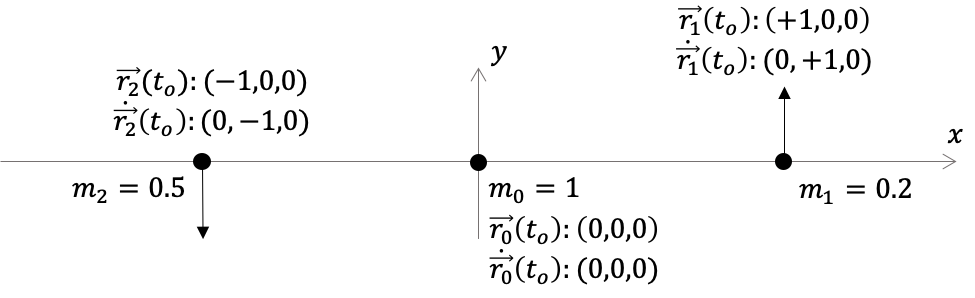
\includegraphics[width=1.0\textwidth]{./figures/horizontal_ncuerpos_ejemplo.png}
\caption{Sistema de tres cuerpos de ejemplo (todas las cantidades están
expresadas en unidades
canónicas)\label{fig:ncuerpos_numerico_ejemplo}}
\end{figure}

Las propiedades del sistema (masas y número de partículas) y las
condiciones iniciales indicadas en la Figura, pueden expresarse, en
términos de las variables auxiliares \(\{Y_k\}\), de la siguiente
manera:

    \begin{code}{}{}\begin{Verbatim}[fontsize=\small,commandchars=\\\{\}]
\PY{c+c1}{\PYZsh{}Número de partículas}
\PY{n}{N}\PY{o}{=}\PY{l+m+mi}{3}
\PY{c+c1}{\PYZsh{}Parámetros gravitacionales o masas de las partúclas}
\PY{n}{mus}\PY{o}{=}\PY{p}{[}\PY{l+m+mf}{1.0}\PY{p}{,}\PY{l+m+mf}{0.2}\PY{p}{,}\PY{l+m+mf}{0.5}\PY{p}{]}
\PY{c+c1}{\PYZsh{}Estado inicial del sistema}
\PY{n}{Y0s}\PY{o}{=}\PY{p}{[}
    \PY{c+c1}{\PYZsh{}Posición cuerpo 0}
    \PY{l+m+mi}{0}\PY{p}{,}\PY{l+m+mi}{0}\PY{p}{,}\PY{l+m+mi}{0}\PY{p}{,}
    \PY{c+c1}{\PYZsh{}Posición cuerpo 1}
    \PY{l+m+mi}{1}\PY{p}{,}\PY{l+m+mi}{0}\PY{p}{,}\PY{l+m+mi}{0}\PY{p}{,}
    \PY{c+c1}{\PYZsh{}Posición cuerpo 2}
    \PY{o}{\PYZhy{}}\PY{l+m+mi}{1}\PY{p}{,}\PY{l+m+mi}{0}\PY{p}{,}\PY{l+m+mi}{0}\PY{p}{,}
    \PY{c+c1}{\PYZsh{}Velocidad cuerpo 0}
    \PY{l+m+mi}{0}\PY{p}{,}\PY{l+m+mi}{0}\PY{p}{,}\PY{l+m+mi}{0}\PY{p}{,}
    \PY{c+c1}{\PYZsh{}Velocidad cuerpo 1}
    \PY{l+m+mi}{0}\PY{p}{,}\PY{l+m+mi}{1}\PY{p}{,}\PY{l+m+mi}{0}\PY{p}{,}
    \PY{c+c1}{\PYZsh{}Velocidad cuerpo 2}
    \PY{l+m+mi}{0}\PY{p}{,}\PY{o}{\PYZhy{}}\PY{l+m+mi}{1}\PY{p}{,}\PY{l+m+mi}{0}\PY{p}{,}
  \PY{p}{]}
\end{Verbatim}

%%

\end{code}

La solución la obtenemos usando \texttt{odeint}:

    \begin{code}{}{}\begin{Verbatim}[fontsize=\small,commandchars=\\\{\}]
\PY{k+kn}{from} \PY{n+nn}{scipy}\PY{n+nn}{.}\PY{n+nn}{integrate} \PY{k}{import} \PY{n}{odeint}
\PY{n}{solucion}\PY{o}{=}\PY{n}{odeint}\PY{p}{(}\PY{n}{edm\PYZus{}ncuerpos}\PY{p}{,}\PY{n}{Y0s}\PY{p}{,}\PY{p}{[}\PY{l+m+mf}{0.0}\PY{p}{,}\PY{l+m+mf}{1.0}\PY{p}{]}\PY{p}{,}\PY{n}{args}\PY{o}{=}\PY{p}{(}\PY{l+m+mi}{3}\PY{p}{,}\PY{n}{mus}\PY{p}{)}\PY{p}{)}
\end{Verbatim}

%%

\end{code}
\vspace{-1em}

%%hidecode


    \begin{Verbatim}[fontsize=\small,commandchars=\\\{\}]
Solución:

array([[ 0.        ,  0.        ,  0.        ,  1.        ,  0.        ,
         0.        , -1.        ,  0.        ,  0.        ,  0.        ,
         0.        ,  0.        ,  0.        ,  1.        ,  0.        ,
         0.        , -1.        ,  0.        ],
       [-0.15068697, -0.06168292,  0.        ,  0.49242022,  0.83105115,
         0.        , -0.49559416, -0.80905462,  0.        , -0.29283302,
        -0.20870151,  0.        , -0.91545262,  0.52712521,  0.        ,
         0.95184709, -0.39344707,  0.        ]])
\end{Verbatim}

La matriz resultante tiene, como filas, el estado de las partículas del
sistema para cada uno de los instantes provistos en el vector de valores
de tiempo (en este caso \texttt{{[}0.0,1.0{]}}). Así, la fila 0 no es
otra cosa que las mismas condiciones iniciales provistas. Por otro lado,
la fila 1 contiene el estado del sistema en el tiempo \(t=1\), que es
justamente la información que necesitabamos obtener.

Las columnas de la matriz de solución, por otro lado, contienen los
valores de la variable auxiliar \(Y_k\), que a su vez corresponden a las
posiciones y velocidades de las partículas, de acuerdo a las reglas
definidas en Ec. (\ref{eq:numerico_variables_auxiliares}). Así, las
columnas 0, 1 y 2, contienen el vector posición de la partícula 0. Las
columnas 3, 4 y 5, la posición de la partícula 1 y las columnas 6, 7 y
8, la posición de la partícula 2. De otro lado, las columnas 9, 10 y 11,
contendrán las componentes de la velocidad de la partícula 0 y así
sucesivamente.

Una forma más apropiada de manipular la matriz solución puede ser
asignar el valor de sus columnas a vectores (o mejor, matrices) con
nombres que nos recuerden el hecho que almacenan posiciones y
velocidades de las diferentes partículas. Así por ejemplo, las
posiciones y velocidades de la partícula 0, en cada uno de los tiempos
en los que se realiza la integración,
\({\vec r}_0(t),\dot{\vec r}_0(t)\), pueden almacenarse usando las
matrices \texttt{r0s} y \texttt{v0s}:

    \begin{code}{}{}\begin{Verbatim}[fontsize=\small,commandchars=\\\{\}]
\PY{n}{r0s}\PY{o}{=}\PY{n}{solucion}\PY{p}{[}\PY{p}{:}\PY{p}{,}\PY{l+m+mi}{0}\PY{p}{:}\PY{l+m+mi}{3}\PY{p}{]}
\PY{n}{v0s}\PY{o}{=}\PY{n}{solucion}\PY{p}{[}\PY{p}{:}\PY{p}{,}\PY{l+m+mi}{9}\PY{p}{:}\PY{l+m+mi}{12}\PY{p}{]}
\end{Verbatim}

%%

\end{code}
\vspace{-1em}

%%hidecode


    \begin{Verbatim}[fontsize=\small,commandchars=\\\{\}]
r\_0(t)
= [[ 0.          0.          0.        ]
 [-0.15068697 -0.06168292  0.        ]]
v\_0(t)
= [[ 0.          0.          0.        ]
 [-0.29283302 -0.20870151  0.        ]]
\end{Verbatim}

En general, las posiciones o velocidades de todas las partículas del
sistema, \({\vec r}_i(t)\), \(\dot{\vec r}_i(t)\), pueden almacenarse en
matrices \texttt{rs} o \texttt{vs}, tal que, para obtener para una
partícula, el valor de una componente del vector posición o de la
velocidad, en un determinado tiempo, la regla será:

\begin{Shaded}
\begin{Highlighting}[]
\NormalTok{  rs[Partícula,Tiempo,Componente]}
\NormalTok{  vs[Partícula,Tiempo,Componente]}
\end{Highlighting}
\end{Shaded}

Así, \texttt{rs{[}0,1,2{]}} corresponderá a la coordenada z (componente
2), en el tiempo 1, para la partícula 0. Por su parte
\texttt{vs{[}1,:,0{]}} serán todos los valores (elipsis \texttt{:}) de
la coordenada \(x\) (componente 0), para la partícula 1.

El algoritmo para convertir la matriz de solución en \texttt{rs} y
\texttt{vs} se presenta a continuacón:

    \begin{code}{Algoritmo}{code:solucion_a_rs_vs}\begin{Verbatim}[fontsize=\small,commandchars=\\\{\}]
\PY{k+kn}{import} \PY{n+nn}{numpy} \PY{k}{as} \PY{n+nn}{np}
\PY{n}{rs}\PY{o}{=}\PY{n}{np}\PY{o}{.}\PY{n}{zeros}\PY{p}{(}\PY{p}{(}\PY{n}{N}\PY{p}{,}\PY{l+m+mi}{2}\PY{p}{,}\PY{l+m+mi}{3}\PY{p}{)}\PY{p}{)}
\PY{n}{vs}\PY{o}{=}\PY{n}{np}\PY{o}{.}\PY{n}{zeros}\PY{p}{(}\PY{p}{(}\PY{n}{N}\PY{p}{,}\PY{l+m+mi}{2}\PY{p}{,}\PY{l+m+mi}{3}\PY{p}{)}\PY{p}{)}
\PY{k}{for} \PY{n}{i} \PY{o+ow}{in} \PY{n+nb}{range}\PY{p}{(}\PY{n}{N}\PY{p}{)}\PY{p}{:}
    \PY{n}{rs}\PY{p}{[}\PY{n}{i}\PY{p}{]}\PY{o}{=}\PY{n}{solucion}\PY{p}{[}\PY{p}{:}\PY{p}{,}\PY{l+m+mi}{3}\PY{o}{*}\PY{n}{i}\PY{p}{:}\PY{l+m+mi}{3}\PY{o}{*}\PY{n}{i}\PY{o}{+}\PY{l+m+mi}{3}\PY{p}{]}
    \PY{n}{vs}\PY{p}{[}\PY{n}{i}\PY{p}{]}\PY{o}{=}\PY{n}{solucion}\PY{p}{[}\PY{p}{:}\PY{p}{,}\PY{l+m+mi}{3}\PY{o}{*}\PY{n}{N}\PY{o}{+}\PY{l+m+mi}{3}\PY{o}{*}\PY{n}{i}\PY{p}{:}\PY{l+m+mi}{3}\PY{o}{*}\PY{n}{N}\PY{o}{+}\PY{l+m+mi}{3}\PY{o}{*}\PY{n}{i}\PY{o}{+}\PY{l+m+mi}{3}\PY{p}{]}
\end{Verbatim}

%%

\end{code}
\vspace{-1em}

%%hidecode


    \begin{Verbatim}[fontsize=\small,commandchars=\\\{\}]
rs = 
[[[ 0.          0.          0.        ]
  [-0.15068697 -0.06168292  0.        ]]

 [[ 1.          0.          0.        ]
  [ 0.49242022  0.83105115  0.        ]]

 [[-1.          0.          0.        ]
  [-0.49559416 -0.80905462  0.        ]]]
vs = 
[[[ 0.          0.          0.        ]
  [-0.29283302 -0.20870151  0.        ]]

 [[ 0.          1.          0.        ]
  [-0.91545262  0.52712521  0.        ]]

 [[ 0.         -1.          0.        ]
  [ 0.95184709 -0.39344707  0.        ]]]
\end{Verbatim}

Finalmente, con la solución parametrizada apropiadamente, podemos
escribir el algoritmo requerido para mostrar, gráficamente la posición
de las partículas en el espacio:
%%HIDE%%
    \begin{code}{Algoritmo}{code:6_ProblemaNCuerpos_17}\begin{Verbatim}[fontsize=\small,commandchars=\\\{\}]
\PY{k+kn}{import} \PY{n+nn}{matplotlib}\PY{n+nn}{.}\PY{n+nn}{pyplot} \PY{k}{as} \PY{n+nn}{plt}
\PY{n}{fig}\PY{o}{=}\PY{n}{plt}\PY{o}{.}\PY{n}{figure}\PY{p}{(}\PY{p}{)}
\PY{n}{ax}\PY{o}{=}\PY{n}{fig}\PY{o}{.}\PY{n}{gca}\PY{p}{(}\PY{p}{)}

\PY{k}{for} \PY{n}{i} \PY{o+ow}{in} \PY{n+nb}{range}\PY{p}{(}\PY{n}{N}\PY{p}{)}\PY{p}{:}
    \PY{n}{ax}\PY{o}{.}\PY{n}{plot}\PY{p}{(}\PY{n}{rs}\PY{p}{[}\PY{n}{i}\PY{p}{,}\PY{p}{:}\PY{p}{,}\PY{l+m+mi}{0}\PY{p}{]}\PY{p}{,}\PY{n}{rs}\PY{p}{[}\PY{n}{i}\PY{p}{,}\PY{p}{:}\PY{p}{,}\PY{l+m+mi}{1}\PY{p}{]}\PY{p}{,}\PY{n}{marker}\PY{o}{=}\PY{l+s+s1}{\PYZsq{}}\PY{l+s+s1}{o}\PY{l+s+s1}{\PYZsq{}}\PY{p}{)}\PY{p}{;}

\PY{k+kn}{from} \PY{n+nn}{pymcel}\PY{n+nn}{.}\PY{n+nn}{plot} \PY{k}{import} \PY{n}{fija\PYZus{}ejes\PYZus{}proporcionales}
\PY{n}{fija\PYZus{}ejes\PYZus{}proporcionales}\PY{p}{(}\PY{n}{ax}\PY{p}{,}\PY{n}{rs}\PY{p}{)}\PY{p}{;}
\end{Verbatim}

%%figcaption::show::Posiciones y velocidades de las partículas en el sistema de ejemplo, en el tiempo inicial y en $t=1$ (en unidades canónicas).

\tcblower
\footnotesize
\em ver Figura \ref{fig:code:6_ProblemaNCuerpos_17}
\end{code}

    \begin{center}

\begin{figure}[ht!]
\centering
    \adjustimage{max size={0.8\linewidth}{0.8\paperheight}}{combined_files/combined_1091_0.png}
\caption{Figura correspondiente al código \ref{code:6_ProblemaNCuerpos_17}. Posiciones y velocidades de las partículas en el sistema de ejemplo, en el tiempo inicial y en $t=1$ (en unidades canónicas).\label{fig:code:6_ProblemaNCuerpos_17}}
\end{figure}

    \end{center}
%{ \hspace*{\fill} \\}
    
Todo el procedimiento descrito en los códigos anteriores, puede
condensarse en pocas líneas, si se diseñan rutinas adecuadas para
convertir las condiciones iniciales de un sistema de partículas en el
vector de valores iniciales de las variables auxiliares \texttt{Y0s} o
para convertir la matriz de solución en las matrices de posición
\texttt{rs} y velocidad \texttt{vs}.

Podemos, por ejemplo, expresar las condiciones iniciales del sistema
usando una estructura de datos más \emph{legible}, p.e. una lista de
diccionarios:

    \begin{code}{}{}\begin{Verbatim}[fontsize=\small,commandchars=\\\{\}]
\PY{n}{sistema\PYZus{}ejemplo}\PY{o}{=}\PY{p}{[}
    \PY{n+nb}{dict}\PY{p}{(}\PY{n}{m}\PY{o}{=}\PY{l+m+mf}{1.0}\PY{p}{,}\PY{n}{r}\PY{o}{=}\PY{p}{[}\PY{l+m+mf}{0.0}\PY{p}{,}\PY{l+m+mf}{0.0}\PY{p}{,}\PY{l+m+mf}{0.0}\PY{p}{]}\PY{p}{,}\PY{n}{v}\PY{o}{=}\PY{p}{[}\PY{l+m+mf}{0.0}\PY{p}{,}\PY{l+m+mf}{0.0}\PY{p}{,}\PY{l+m+mf}{0.0}\PY{p}{]}\PY{p}{)}\PY{p}{,}
    \PY{n+nb}{dict}\PY{p}{(}\PY{n}{m}\PY{o}{=}\PY{l+m+mf}{0.2}\PY{p}{,}\PY{n}{r}\PY{o}{=}\PY{p}{[}\PY{l+m+mf}{1.0}\PY{p}{,}\PY{l+m+mf}{0.0}\PY{p}{,}\PY{l+m+mf}{0.0}\PY{p}{]}\PY{p}{,}\PY{n}{v}\PY{o}{=}\PY{p}{[}\PY{l+m+mf}{0.0}\PY{p}{,}\PY{l+m+mf}{1.0}\PY{p}{,}\PY{l+m+mf}{0.0}\PY{p}{]}\PY{p}{)}\PY{p}{,}
    \PY{n+nb}{dict}\PY{p}{(}\PY{n}{m}\PY{o}{=}\PY{l+m+mf}{0.5}\PY{p}{,}\PY{n}{r}\PY{o}{=}\PY{p}{[}\PY{o}{\PYZhy{}}\PY{l+m+mf}{1.0}\PY{p}{,}\PY{l+m+mf}{0.0}\PY{p}{,}\PY{l+m+mf}{0.0}\PY{p}{]}\PY{p}{,}\PY{n}{v}\PY{o}{=}\PY{p}{[}\PY{l+m+mf}{0.0}\PY{p}{,}\PY{o}{\PYZhy{}}\PY{l+m+mf}{1.0}\PY{p}{,}\PY{l+m+mf}{0.0}\PY{p}{]}\PY{p}{)}\PY{p}{,}
\PY{p}{]}
\end{Verbatim}

%%

\end{code}

Para convertir esta estructura en el vector con las condiciones
iniciales de las variables auxiliares usaremos la siguiente rutina:

    \begin{code}{Algoritmo}{code:sistema_a_Y}\begin{Verbatim}[fontsize=\small,commandchars=\\\{\}]
\PY{k}{def} \PY{n+nf}{sistema\PYZus{}a\PYZus{}Y}\PY{p}{(}\PY{n}{sistema}\PY{p}{)}\PY{p}{:}
    \PY{n}{mus}\PY{o}{=}\PY{p}{[}\PY{p}{]}
    \PY{n}{r0s}\PY{o}{=}\PY{p}{[}\PY{p}{]}
    \PY{n}{v0s}\PY{o}{=}\PY{p}{[}\PY{p}{]}
    \PY{n}{N}\PY{o}{=}\PY{l+m+mi}{0}
    \PY{k}{for} \PY{n}{particula} \PY{o+ow}{in} \PY{n}{sistema}\PY{p}{:}
        \PY{n}{m}\PY{o}{=}\PY{n}{particula}\PY{p}{[}\PY{l+s+s1}{\PYZsq{}}\PY{l+s+s1}{m}\PY{l+s+s1}{\PYZsq{}}\PY{p}{]}
        \PY{k}{if} \PY{n}{m}\PY{o}{\PYZgt{}}\PY{l+m+mi}{0}\PY{p}{:}
            \PY{n}{mus}\PY{o}{+}\PY{o}{=}\PY{p}{[}\PY{n}{m}\PY{p}{]}
            \PY{n}{r0s}\PY{o}{+}\PY{o}{=}\PY{n+nb}{list}\PY{p}{(}\PY{n}{particula}\PY{p}{[}\PY{l+s+s2}{\PYZdq{}}\PY{l+s+s2}{r}\PY{l+s+s2}{\PYZdq{}}\PY{p}{]}\PY{p}{)}
            \PY{n}{v0s}\PY{o}{+}\PY{o}{=}\PY{n+nb}{list}\PY{p}{(}\PY{n}{particula}\PY{p}{[}\PY{l+s+s2}{\PYZdq{}}\PY{l+s+s2}{v}\PY{l+s+s2}{\PYZdq{}}\PY{p}{]}\PY{p}{)}
            \PY{n}{N}\PY{o}{+}\PY{o}{=}\PY{l+m+mi}{1}
    \PY{k+kn}{from} \PY{n+nn}{numpy} \PY{k}{import} \PY{n}{array}
    \PY{n}{Y0s}\PY{o}{=}\PY{n}{array}\PY{p}{(}\PY{n}{r0s}\PY{o}{+}\PY{n}{v0s}\PY{p}{)}
    \PY{n}{mus}\PY{o}{=}\PY{n}{array}\PY{p}{(}\PY{n}{mus}\PY{p}{)}
    \PY{k}{return} \PY{n}{N}\PY{p}{,}\PY{n}{mus}\PY{p}{,}\PY{n}{Y0s}
\end{Verbatim}

%%

\end{code}

Nótese que en la rutina hemos usado inicialmente listas (p.e.
\texttt{mus={[}{]}}) pero para devolver el resultado de la rutina,
convertirmos esas listas en arreglos de \texttt{NumPy} (p.e.
\texttt{mus=array(mus)}) que tienen propiedades más adecuadas para su
manipulación posterior. También debe tenerse cuidado con la línea
\texttt{Y0s=array(rs+vs)} donde se da a entender que estamos
\emph{sumando} posiciones y velocidades (peras con manzanas.) Debemos
recordar aquí (ver la \autoref{conjuntos_tuplas_vectores}) que dado
que en el algoritmo \texttt{rs} y \texttt{vs} son listas, la suma indica
la unión de esas listas (para formar la lista \texttt{Y0s}) y no la suma
vectorial de ellas.

Un último detalle codificado en la rutina \texttt{sistema\_a\_Y} (que
usaremos mucho en lo que queda de este libro) es que si la masa de una
partícula en el diccionario \texttt{sistema} se fija en 0, la partícula
no será incluída en las condiciones iniciales (esa es justamente la
función del condicional que comienza con
\texttt{if\ m\textgreater{}0:...}.) Esta condición puede ser de utilidad
para agregar y quitar partículas a un sistema sin necesidad de borrar o
comentar sus condiciones iniciales en el diccionario de
\texttt{sistema}.

Por otro lado, para convertir la matriz \texttt{solucion} en matrices de
posición y velocidad, \texttt{rs} y \texttt{vs}, tal y como lo hicimos
en el Alg. (\ref{code:solucion_a_rs_vs}), usaremos la siguiente rutina:

    \begin{code}{Algoritmo}{code:solucion_a_estado}\begin{Verbatim}[fontsize=\small,commandchars=\\\{\}]
\PY{k}{def} \PY{n+nf}{solucion\PYZus{}a\PYZus{}estado}\PY{p}{(}\PY{n}{solucion}\PY{p}{,}\PY{n}{Nparticulas}\PY{p}{,}\PY{n}{Ntiempos}\PY{p}{)}\PY{p}{:}
    \PY{k+kn}{from} \PY{n+nn}{numpy} \PY{k}{import} \PY{n}{zeros}
    \PY{n}{rs}\PY{o}{=}\PY{n}{zeros}\PY{p}{(}\PY{p}{(}\PY{n}{Nparticulas}\PY{p}{,}\PY{n}{Ntiempos}\PY{p}{,}\PY{l+m+mi}{3}\PY{p}{)}\PY{p}{)}
    \PY{n}{vs}\PY{o}{=}\PY{n}{zeros}\PY{p}{(}\PY{p}{(}\PY{n}{Nparticulas}\PY{p}{,}\PY{n}{Ntiempos}\PY{p}{,}\PY{l+m+mi}{3}\PY{p}{)}\PY{p}{)}
    \PY{k}{for} \PY{n}{i} \PY{o+ow}{in} \PY{n+nb}{range}\PY{p}{(}\PY{n}{Nparticulas}\PY{p}{)}\PY{p}{:}
        \PY{n}{rs}\PY{p}{[}\PY{n}{i}\PY{p}{]}\PY{o}{=}\PY{n}{solucion}\PY{p}{[}\PY{p}{:}\PY{p}{,}\PY{l+m+mi}{3}\PY{o}{*}\PY{n}{i}\PY{p}{:}\PY{l+m+mi}{3}\PY{o}{*}\PY{n}{i}\PY{o}{+}\PY{l+m+mi}{3}\PY{p}{]}
        \PY{n}{vs}\PY{p}{[}\PY{n}{i}\PY{p}{]}\PY{o}{=}\PY{n}{solucion}\PY{p}{[}\PY{p}{:}\PY{p}{,}\PY{l+m+mi}{3}\PY{o}{*}\PY{n}{Nparticulas}\PY{o}{+}\PY{l+m+mi}{3}\PY{o}{*}\PY{n}{i}\PY{p}{:}\PY{l+m+mi}{3}\PY{o}{*}\PY{n}{Nparticulas}\PY{o}{+}\PY{l+m+mi}{3}\PY{o}{*}\PY{n}{i}\PY{o}{+}\PY{l+m+mi}{3}\PY{p}{]}
    \PY{k}{return} \PY{n}{rs}\PY{p}{,}\PY{n}{vs}
\end{Verbatim}

%%

\end{code}

Con todos estos elementos a la mano, un algoritmo completo para expresar
las condiciones iniciales del sistema en
\autoref{fig:ncuerpos_numerico_ejemplo}, encontrar la solución numérica
a las e.d.m.r. para 50 valores del tiempo entre \(t_0=0.0\) y \(t=5.0\)
(en unidades canónicas) y visualizar la solución, será:

    \begin{code}{Algoritmo}{code:ncuerpos_ejemplo1}\begin{Verbatim}[fontsize=\small,commandchars=\\\{\}]
\PY{c+c1}{\PYZsh{} Definición de las condiciones iniciales }
\PY{n}{sistema\PYZus{}ejemplo}\PY{o}{=}\PY{p}{[}
    \PY{n+nb}{dict}\PY{p}{(}\PY{n}{m}\PY{o}{=}\PY{l+m+mf}{1.0}\PY{p}{,}\PY{n}{r}\PY{o}{=}\PY{p}{[}\PY{l+m+mf}{0.0}\PY{p}{,}\PY{l+m+mf}{0.0}\PY{p}{,}\PY{l+m+mf}{0.0}\PY{p}{]}\PY{p}{,}\PY{n}{v}\PY{o}{=}\PY{p}{[}\PY{l+m+mf}{0.0}\PY{p}{,}\PY{l+m+mf}{0.0}\PY{p}{,}\PY{l+m+mf}{0.0}\PY{p}{]}\PY{p}{)}\PY{p}{,}
    \PY{n+nb}{dict}\PY{p}{(}\PY{n}{m}\PY{o}{=}\PY{l+m+mf}{0.2}\PY{p}{,}\PY{n}{r}\PY{o}{=}\PY{p}{[}\PY{l+m+mf}{1.0}\PY{p}{,}\PY{l+m+mf}{0.0}\PY{p}{,}\PY{l+m+mf}{0.0}\PY{p}{]}\PY{p}{,}\PY{n}{v}\PY{o}{=}\PY{p}{[}\PY{l+m+mf}{0.0}\PY{p}{,}\PY{l+m+mf}{1.0}\PY{p}{,}\PY{l+m+mf}{0.0}\PY{p}{]}\PY{p}{)}\PY{p}{,}
    \PY{n+nb}{dict}\PY{p}{(}\PY{n}{m}\PY{o}{=}\PY{l+m+mf}{0.5}\PY{p}{,}\PY{n}{r}\PY{o}{=}\PY{p}{[}\PY{o}{\PYZhy{}}\PY{l+m+mf}{1.0}\PY{p}{,}\PY{l+m+mf}{0.0}\PY{p}{,}\PY{l+m+mf}{0.0}\PY{p}{]}\PY{p}{,}\PY{n}{v}\PY{o}{=}\PY{p}{[}\PY{l+m+mf}{0.0}\PY{p}{,}\PY{o}{\PYZhy{}}\PY{l+m+mf}{1.0}\PY{p}{,}\PY{l+m+mf}{0.0}\PY{p}{]}\PY{p}{)}\PY{p}{,}
\PY{p}{]}
\PY{n}{N}\PY{p}{,}\PY{n}{mus}\PY{p}{,}\PY{n}{Yo}\PY{o}{=}\PY{n}{sistema\PYZus{}a\PYZus{}Y}\PY{p}{(}\PY{n}{sistema\PYZus{}ejemplo}\PY{p}{)}

\PY{c+c1}{\PYZsh{}Tiempo de integración}
\PY{k+kn}{import} \PY{n+nn}{numpy} \PY{k}{as} \PY{n+nn}{np}
\PY{n}{Nt}\PY{o}{=}\PY{l+m+mi}{50}
\PY{n}{ts}\PY{o}{=}\PY{n}{np}\PY{o}{.}\PY{n}{linspace}\PY{p}{(}\PY{l+m+mf}{0.0}\PY{p}{,}\PY{l+m+mi}{5}\PY{p}{,}\PY{n}{Nt}\PY{p}{,}\PY{n}{endpoint}\PY{o}{=}\PY{k+kc}{True}\PY{p}{)}

\PY{c+c1}{\PYZsh{} Solución al sistema de ecuaciones diferenciales}
\PY{k+kn}{from} \PY{n+nn}{scipy}\PY{n+nn}{.}\PY{n+nn}{integrate} \PY{k}{import} \PY{n}{odeint}
\PY{n}{solucion\PYZus{}ejemplo}\PY{o}{=}\PY{n}{odeint}\PY{p}{(}\PY{n}{edm\PYZus{}ncuerpos}\PY{p}{,}\PY{n}{Yo}\PY{p}{,}\PY{n}{ts}\PY{p}{,}\PY{n}{args}\PY{o}{=}\PY{p}{(}\PY{n}{N}\PY{p}{,}\PY{n}{mus}\PY{p}{)}\PY{p}{)}
\PY{n}{rs}\PY{p}{,}\PY{n}{vs}\PY{o}{=}\PY{n}{solucion\PYZus{}a\PYZus{}estado}\PY{p}{(}\PY{n}{solucion\PYZus{}ejemplo}\PY{p}{,}\PY{n}{N}\PY{p}{,}\PY{n}{Nt}\PY{p}{)}

\PY{c+c1}{\PYZsh{} Componente gráfica del algoritmo}
\PY{k+kn}{import} \PY{n+nn}{matplotlib}\PY{n+nn}{.}\PY{n+nn}{pyplot} \PY{k}{as} \PY{n+nn}{plt}
\PY{n}{fig}\PY{o}{=}\PY{n}{plt}\PY{o}{.}\PY{n}{figure}\PY{p}{(}\PY{p}{)}
\PY{n}{ax}\PY{o}{=}\PY{n}{fig}\PY{o}{.}\PY{n}{gca}\PY{p}{(}\PY{p}{)}

\PY{k}{for} \PY{n}{i} \PY{o+ow}{in} \PY{n+nb}{range}\PY{p}{(}\PY{n}{N}\PY{p}{)}\PY{p}{:}
    \PY{n}{ax}\PY{o}{.}\PY{n}{plot}\PY{p}{(}\PY{n}{rs}\PY{p}{[}\PY{n}{i}\PY{p}{,}\PY{p}{:}\PY{p}{,}\PY{l+m+mi}{0}\PY{p}{]}\PY{p}{,}\PY{n}{rs}\PY{p}{[}\PY{n}{i}\PY{p}{,}\PY{p}{:}\PY{p}{,}\PY{l+m+mi}{1}\PY{p}{]}\PY{p}{,}\PY{n}{marker}\PY{o}{=}\PY{l+s+s1}{\PYZsq{}}\PY{l+s+s1}{o}\PY{l+s+s1}{\PYZsq{}}\PY{p}{)}\PY{p}{;}

\PY{k+kn}{from} \PY{n+nn}{pymcel}\PY{n+nn}{.}\PY{n+nn}{plot} \PY{k}{import} \PY{n}{fija\PYZus{}ejes\PYZus{}proporcionales}
\PY{n}{fija\PYZus{}ejes\PYZus{}proporcionales}\PY{p}{(}\PY{n}{ax}\PY{p}{,}\PY{n}{rs}\PY{p}{)}\PY{p}{;}
\end{Verbatim}

%%figcaption::show::Posiciones y velocidades de las partículas en el sistema de ejemplo, entre el tiempo inicial $t_0=0$ y $t=5$ (en unidades canónicas).

\tcblower
\footnotesize
\em ver Figura \ref{fig:code:ncuerpos_ejemplo1}
\end{code}

    \begin{center}

\begin{figure}[ht!]
\centering
    \adjustimage{max size={0.8\linewidth}{0.8\paperheight}}{combined_files/combined_1100_0.png}
\caption{Figura correspondiente al código \ref{code:ncuerpos_ejemplo1}. Posiciones y velocidades de las partículas en el sistema de ejemplo, entre el tiempo inicial $t_0=0$ y $t=5$ (en unidades canónicas).\label{fig:code:ncuerpos_ejemplo1}}
\end{figure}

    \end{center}
%{ \hspace*{\fill} \\}
    
Puede encontrar una versión animada o interactiva de este gráfico en la
\autoref{ncuerpos_numerico_interactivas} al final de esta sección.

Dado que en general, el movimiento de los cuerpos en un sistema de
muchas partículas, ocurre en el espacio de tres dimensiones, la
componente gráfica del algortimo anterior puede reemplazarse con este
código:

    \begin{code}{Algoritmo}{code:plot_ncuerpos_3d}\begin{Verbatim}[fontsize=\small,commandchars=\\\{\}]
\PY{k}{def} \PY{n+nf}{plot\PYZus{}ncuerpos\PYZus{}3d}\PY{p}{(}\PY{n}{rs}\PY{p}{,}\PY{n}{vs}\PY{p}{,}\PY{o}{*}\PY{o}{*}\PY{n}{opciones}\PY{p}{)}\PY{p}{:}
    \PY{c+c1}{\PYZsh{}Número de partículas}
    \PY{n}{N}\PY{o}{=}\PY{n}{rs}\PY{o}{.}\PY{n}{shape}\PY{p}{[}\PY{l+m+mi}{0}\PY{p}{]}
    
    \PY{k+kn}{import} \PY{n+nn}{matplotlib}\PY{n+nn}{.}\PY{n+nn}{pyplot} \PY{k}{as} \PY{n+nn}{plt}
    \PY{k+kn}{from} \PY{n+nn}{mpl\PYZus{}toolkits}\PY{n+nn}{.}\PY{n+nn}{mplot3d} \PY{k}{import} \PY{n}{Axes3D}
    \PY{n}{fig}\PY{o}{=}\PY{n}{plt}\PY{o}{.}\PY{n}{figure}\PY{p}{(}\PY{p}{)}
    \PY{n}{ax}\PY{o}{=}\PY{n}{fig}\PY{o}{.}\PY{n}{gca}\PY{p}{(}\PY{n}{projection}\PY{o}{=}\PY{l+s+s1}{\PYZsq{}}\PY{l+s+s1}{3d}\PY{l+s+s1}{\PYZsq{}}\PY{p}{)}

    \PY{k}{for} \PY{n}{i} \PY{o+ow}{in} \PY{n+nb}{range}\PY{p}{(}\PY{n}{N}\PY{p}{)}\PY{p}{:}
        \PY{n}{ax}\PY{o}{.}\PY{n}{plot}\PY{p}{(}\PY{n}{rs}\PY{p}{[}\PY{n}{i}\PY{p}{,}\PY{p}{:}\PY{p}{,}\PY{l+m+mi}{0}\PY{p}{]}\PY{p}{,}\PY{n}{rs}\PY{p}{[}\PY{n}{i}\PY{p}{,}\PY{p}{:}\PY{p}{,}\PY{l+m+mi}{1}\PY{p}{]}\PY{p}{,}\PY{n}{rs}\PY{p}{[}\PY{n}{i}\PY{p}{,}\PY{p}{:}\PY{p}{,}\PY{l+m+mi}{2}\PY{p}{]}\PY{p}{,}\PY{o}{*}\PY{o}{*}\PY{n}{opciones}\PY{p}{)}\PY{p}{;}

    \PY{k+kn}{from} \PY{n+nn}{pymcel}\PY{n+nn}{.}\PY{n+nn}{plot} \PY{k}{import} \PY{n}{fija\PYZus{}ejes3d\PYZus{}proporcionales}
    \PY{n}{fija\PYZus{}ejes3d\PYZus{}proporcionales}\PY{p}{(}\PY{n}{ax}\PY{p}{)}\PY{p}{;}
    \PY{n}{fig}\PY{o}{.}\PY{n}{tight\PYZus{}layout}\PY{p}{(}\PY{p}{)}\PY{p}{;}
    \PY{n}{plt}\PY{o}{.}\PY{n}{show}\PY{p}{(}\PY{p}{)}\PY{p}{;}
    \PY{k}{return} \PY{n}{fig}
\end{Verbatim}

%%

\end{code}

Que invocamos con:

    \begin{code}{Algoritmo}{code:6_ProblemaNCuerpos_18}\begin{Verbatim}[fontsize=\small,commandchars=\\\{\}]
\PY{n}{fig}\PY{o}{=}\PY{n}{plot\PYZus{}ncuerpos\PYZus{}3d}\PY{p}{(}\PY{n}{rs}\PY{p}{,}\PY{n}{vs}\PY{p}{,}\PY{n}{marker}\PY{o}{=}\PY{l+s+s1}{\PYZsq{}}\PY{l+s+s1}{.}\PY{l+s+s1}{\PYZsq{}}\PY{p}{)}\PY{p}{;}
\end{Verbatim}

%%

\tcblower
\footnotesize
\em ver Figura \ref{fig:code:6_ProblemaNCuerpos_18}
\end{code}

    \begin{center}

\begin{figure}[ht!]
\centering
    \adjustimage{max size={0.8\linewidth}{0.8\paperheight}}{combined_files/combined_1105_0.png}
\caption{Figura correspondiente al código \ref{code:6_ProblemaNCuerpos_18}.\label{fig:code:6_ProblemaNCuerpos_18}}
\end{figure}

    \end{center}
%{ \hspace*{\fill} \\}
    
La diferencia de la representación en tres dimensiones de los sistemas,
de su representación en dos dimensiones esta en:

\begin{itemize}
\item
  El uso del módulo \texttt{Axes3D}:
  \texttt{from\ mpl\_toolkits.mplot3d\ import\ Axes3D}.
\item
  La elección de una proyección específica al definir el espacio de
  graficación:
  \texttt{ax=fig.gca(projection=\textquotesingle{}3d\textquotesingle{})}.
\item
  El uso de las coordenadas \(x,y,z\) de las posiciones de las
  partículas, en lugar de solo dos de ellas:

\begin{Shaded}
\begin{Highlighting}[]
\NormalTok{ax.plot(rs[i,:,}\DecValTok{0}\NormalTok{],rs[i,:,}\DecValTok{1}\NormalTok{],rs[i,:,}\DecValTok{2}\NormalTok{],marker}\OperatorTok{=}\StringTok{'o'}\NormalTok{)}\OperatorTok{;}
\end{Highlighting}
\end{Shaded}
\item
  Y el ajuste de las escalas de los tres ejes a través de una rutina
  previamente preparada en el paquete \texttt{pymcel}:
  \texttt{fija\_ejes3d\_proporcionales(ax)}.
\end{itemize}

\hypertarget{ncuerpos_numerico_interactivas}{%
\subsection{Figuras interactivas}\label{ncuerpos_numerico_interactivas}}

Busque las figuras interactivas y las animaciones incluídas en el
\hreffoot{http://seap-udea.org/MecanicaCeleste_Zuluaga}{sitio en línea del
libro}.

\hypertarget{ncuerpos_numerico_constantes_virial}{%
\subsection{Constantes de movimiento y teorema del
virial}\label{ncuerpos_numerico_constantes_virial}}

Una interesante primera ``aplicación'' de la solución numérica al
problema de los N cuerpos vista en estas secciones, es la de verificar
``experimentalmente'' los resultados analíticos descritos en la
\autoref{solucione_analitica} y en la \autoref{ncuerpos_virial}.

Para ello estudiaremos un sistema de 5 partículas con masas, posiciones
y velocidades generadas al azar. La solución numérica a las e.d.m.r. del
sistema, obtenida con los métodos vistos en esta sección, nos permitirá
obtener las listas de sus posiciones y velocidades para distintos
valores del tiempo. Con estas listas podremos calcular y graficar los
valores de las constantes de movimiento, momento lineal, momento
angular, energía y de las cantidades críticas para el teorema del
virial.

Comencemos pues por generar las condiciones iniciales del sistema
usando, entre otras cosas, la rutina \texttt{sistema\_a\_Y} del Alg.
(\ref{code:sistema_a_Y}) y las rutinas de generación de números
aleatorios que usamos en la \autoref{centro_masa}:
%%HIDE%%%%HIDE%%
    \begin{code}{Algoritmo}{code:ncuerpos_constantes_condiciones_iniciales}\begin{Verbatim}[fontsize=\small,commandchars=\\\{\}]
\PY{c+c1}{\PYZsh{}Número de partículas}
\PY{n}{N}\PY{o}{=}\PY{l+m+mi}{5}

\PY{c+c1}{\PYZsh{}Generación de las condiciones para cada partícula}
\PY{k+kn}{from} \PY{n+nn}{numpy}\PY{n+nn}{.}\PY{n+nn}{random} \PY{k}{import} \PY{n}{uniform}\PY{p}{,}\PY{n}{seed}
\PY{n}{seed}\PY{p}{(}\PY{l+m+mi}{7}\PY{p}{)}

\PY{c+c1}{\PYZsh{}Condiciones iniciales}
\PY{n}{sistema}\PY{o}{=}\PY{p}{[}\PY{p}{]}
\PY{k}{for} \PY{n}{i} \PY{o+ow}{in} \PY{n+nb}{range}\PY{p}{(}\PY{n}{N}\PY{p}{)}\PY{p}{:}
    \PY{n}{particula}\PY{o}{=}\PY{n+nb}{dict}\PY{p}{(}
        \PY{n}{m}\PY{o}{=}\PY{n}{uniform}\PY{p}{(}\PY{l+m+mf}{0.0}\PY{p}{,}\PY{l+m+mf}{1.0}\PY{p}{)}\PY{p}{,}
        \PY{n}{r}\PY{o}{=}\PY{n}{uniform}\PY{p}{(}\PY{o}{\PYZhy{}}\PY{l+m+mf}{1.0}\PY{p}{,}\PY{l+m+mf}{1.0}\PY{p}{,}\PY{n}{size}\PY{o}{=}\PY{l+m+mi}{3}\PY{p}{)}\PY{p}{,}
        \PY{n}{v}\PY{o}{=}\PY{n}{uniform}\PY{p}{(}\PY{o}{\PYZhy{}}\PY{l+m+mf}{1.0}\PY{p}{,}\PY{l+m+mf}{1.0}\PY{p}{,}\PY{n}{size}\PY{o}{=}\PY{l+m+mi}{3}\PY{p}{)}
    \PY{p}{)}
    \PY{n}{sistema}\PY{o}{+}\PY{o}{=}\PY{p}{[}\PY{n}{particula}\PY{p}{]}

\PY{n}{N}\PY{p}{,}\PY{n}{mus}\PY{p}{,}\PY{n}{Y0s}\PY{o}{=}\PY{n}{sistema\PYZus{}a\PYZus{}Y}\PY{p}{(}\PY{n}{sistema}\PY{p}{)}

\PY{c+c1}{\PYZsh{}Tiempos}
\PY{k+kn}{from} \PY{n+nn}{numpy} \PY{k}{import} \PY{n}{linspace}
\PY{n}{Nt}\PY{o}{=}\PY{l+m+mi}{100}
\PY{n}{ts}\PY{o}{=}\PY{n}{linspace}\PY{p}{(}\PY{l+m+mf}{0.0}\PY{p}{,}\PY{l+m+mf}{10.0}\PY{p}{,}\PY{n}{Nt}\PY{p}{)}
\end{Verbatim}

%%

\end{code}

    \begin{code}{}{}\begin{Verbatim}[fontsize=\small,commandchars=\\\{\}]
\PY{n+nb}{print}\PY{p}{(}\PY{n}{f}\PY{l+s+s2}{\PYZdq{}}\PY{l+s+s2}{N = }\PY{l+s+si}{\PYZob{}N\PYZcb{}}\PY{l+s+s2}{\PYZdq{}}\PY{p}{)}
\PY{n+nb}{print}\PY{p}{(}\PY{n}{f}\PY{l+s+s2}{\PYZdq{}}\PY{l+s+s2}{mus = }\PY{l+s+si}{\PYZob{}mus\PYZcb{}}\PY{l+s+s2}{\PYZdq{}}\PY{p}{)}
\PY{n+nb}{print}\PY{p}{(}\PY{n}{f}\PY{l+s+s2}{\PYZdq{}}\PY{l+s+s2}{Y0s = }\PY{l+s+si}{\PYZob{}Y0s\PYZcb{}}\PY{l+s+s2}{\PYZdq{}}\PY{p}{)}
\end{Verbatim}

%%

\end{code}

    \begin{Verbatim}[fontsize=\small,commandchars=\\\{\}]
N = 5
mus = [0.07630829 0.07205113 0.2881456  0.9501295  0.66901324]
Y0s = [ 5.59837584e-01 -1.23181537e-01  4.46930356e-01 -4.63122040e-01
 -2.34998349e-04  3.58459992e-01  8.19187055e-01 -5.73229293e-01
 -9.57520764e-02 -5.39394242e-01  9.69798385e-02  8.18256750e-01
 -6.44942805e-02 -5.90301819e-01 -1.84682218e-02  9.55979024e-01
  7.69917408e-02  2.24092732e-03  6.07478072e-01 -2.38117734e-01
 -8.68127306e-01  8.62412039e-01 -9.50201545e-01  2.01097835e-01
 -7.33661108e-01  4.68251613e-02  5.00819718e-01 -2.55230621e-01
 -4.51976903e-02 -2.68219228e-01]
\end{Verbatim}

Ahora podemos resolver las ecuaciones de movimiento y extraer las
posiciones y velocidades de las partículas:

    \begin{code}{}{}\begin{Verbatim}[fontsize=\small,commandchars=\\\{\}]
\PY{c+c1}{\PYZsh{}Solución}
\PY{k+kn}{from} \PY{n+nn}{scipy}\PY{n+nn}{.}\PY{n+nn}{integrate} \PY{k}{import} \PY{n}{odeint}
\PY{n}{solucion}\PY{o}{=}\PY{n}{odeint}\PY{p}{(}\PY{n}{edm\PYZus{}ncuerpos}\PY{p}{,}\PY{n}{Y0s}\PY{p}{,}\PY{n}{ts}\PY{p}{,}\PY{n}{args}\PY{o}{=}\PY{p}{(}\PY{n}{N}\PY{p}{,}\PY{n}{mus}\PY{p}{)}\PY{p}{)}

\PY{c+c1}{\PYZsh{}Extracción de las posiciones y velocidades}
\PY{n}{rs}\PY{p}{,}\PY{n}{vs}\PY{o}{=}\PY{n}{solucion\PYZus{}a\PYZus{}estado}\PY{p}{(}\PY{n}{solucion}\PY{p}{,}\PY{n}{N}\PY{p}{,}\PY{n}{Nt}\PY{p}{)}
\end{Verbatim}

%%

\end{code}

Una gráfica del movimiento de las partículas en tres dimensiones se
puede obtener usando la rutina \texttt{plot\_ncuerpos\_3d} que definimos
en el Alg. (\ref{code:plot_ncuerpos_3d}):
%%HIDE%%
    \begin{code}{Algoritmo}{code:ncuerpos_ejemplo2}\begin{Verbatim}[fontsize=\small,commandchars=\\\{\}]
\PY{n}{fig}\PY{o}{=}\PY{n}{plot\PYZus{}ncuerpos\PYZus{}3d}\PY{p}{(}\PY{n}{rs}\PY{p}{,}\PY{n}{vs}\PY{p}{,}\PY{n}{marker}\PY{o}{=}\PY{l+s+s1}{\PYZsq{}}\PY{l+s+s1}{.}\PY{l+s+s1}{\PYZsq{}}\PY{p}{)}\PY{p}{;}
\end{Verbatim}

%%

\tcblower
\footnotesize
\em ver Figura \ref{fig:code:ncuerpos_ejemplo2}
\end{code}

    \begin{center}

\begin{figure}[ht!]
\centering
    \adjustimage{max size={0.8\linewidth}{0.8\paperheight}}{combined_files/combined_1121_0.png}
\caption{Figura correspondiente al código \ref{code:ncuerpos_ejemplo2}.\label{fig:code:ncuerpos_ejemplo2}}
\end{figure}

    \end{center}
%{ \hspace*{\fill} \\}
    
Ahora podemos calcular las constantes de movimiento. En este caso, sin
embargo, la dificultad algorítmica estriba en que las posiciones y
velocidades de las partículas están guardadas en las matrices
\texttt{rs} y \texttt{vs} que no son triviales de manipular.

Así, por ejemplo el momento lineal inicial de la partícula 0 esta dado
por:

    \begin{code}{}{}\begin{Verbatim}[fontsize=\small,commandchars=\\\{\}]
\PY{n}{p\PYZus{}0\PYZus{}0}\PY{o}{=}\PY{n}{mus}\PY{p}{[}\PY{l+m+mi}{0}\PY{p}{]}\PY{o}{*}\PY{n}{vs}\PY{p}{[}\PY{l+m+mi}{0}\PY{p}{,}\PY{l+m+mi}{0}\PY{p}{,}\PY{p}{:}\PY{p}{]}
\end{Verbatim}

%%

\end{code}
\vspace{-1em}

%%hidecode


    \begin{Verbatim}[fontsize=\small,commandchars=\\\{\}]
p\_0\_0 = [0.07294912 0.00587511 0.000171  ]
\end{Verbatim}

Pero si queremos el momento lineal de esa partícula en cualquier tiempo
será:

    \begin{code}{}{}\begin{Verbatim}[fontsize=\small,commandchars=\\\{\}]
\PY{n}{p\PYZus{}0}\PY{o}{=}\PY{n}{mus}\PY{p}{[}\PY{l+m+mi}{0}\PY{p}{]}\PY{o}{*}\PY{n}{vs}\PY{p}{[}\PY{l+m+mi}{0}\PY{p}{,}\PY{p}{:}\PY{p}{,}\PY{p}{:}\PY{p}{]}
\end{Verbatim}

%%

\end{code}
\vspace{-1em}

%%hidecode


    \begin{Verbatim}[fontsize=\small,commandchars=\\\{\}]
p\_0(t) = 
[[ 0.07294912  0.00587511  0.000171  ]
 [ 0.0653799   0.00154574 -0.00381787]
 [ 0.05898078 -0.00240643 -0.0070324 ]
 [ 0.05337202 -0.00601935 -0.00963238]
 [ 0.04832467 -0.00932501 -0.0117392 ]]
{\ldots}
\end{Verbatim}

La cuadratura de momento lineal total \(C_{P_\mathrm{CM}}\) la podemos
obtener si sumamos uno a uno los momentos lineales en cada tiempo de
todas las partículas del sistema:

    \begin{code}{}{}\begin{Verbatim}[fontsize=\small,commandchars=\\\{\}]
\PY{k+kn}{from} \PY{n+nn}{numpy} \PY{k}{import} \PY{n}{zeros}
\PY{n}{C\PYZus{}PCM}\PY{o}{=}\PY{n}{zeros}\PY{p}{(}\PY{p}{(}\PY{n}{Nt}\PY{p}{,}\PY{l+m+mi}{3}\PY{p}{)}\PY{p}{)}
\PY{k}{for} \PY{n}{i} \PY{o+ow}{in} \PY{n+nb}{range}\PY{p}{(}\PY{n}{N}\PY{p}{)}\PY{p}{:}
    \PY{n}{C\PYZus{}PCM}\PY{o}{=}\PY{n}{C\PYZus{}PCM}\PY{o}{+}\PY{n}{mus}\PY{p}{[}\PY{n}{i}\PY{p}{]}\PY{o}{*}\PY{n}{vs}\PY{p}{[}\PY{n}{i}\PY{p}{,}\PY{p}{:}\PY{p}{,}\PY{p}{:}\PY{p}{]}
\end{Verbatim}

%%

\end{code}
\vspace{-1em}

%%hidecode


    \begin{Verbatim}[fontsize=\small,commandchars=\\\{\}]
C\_PCM = 
[[-0.50260689 -0.27082582  0.29196827]
 [-0.50260689 -0.27082582  0.29196827]
 [-0.50260689 -0.27082582  0.29196827]
 [-0.50260689 -0.27082582  0.29196827]
 [-0.50260689 -0.27082582  0.29196827]]
{\ldots}
\end{Verbatim}

Y como vemos el valor del momento lineal es el mismo, que es lo que
esperabamos de acuerdo con la teoría.

Por otro lado la cuadratura de momento angular será:

    \begin{code}{}{}\begin{Verbatim}[fontsize=\small,commandchars=\\\{\}]
\PY{k+kn}{from} \PY{n+nn}{numpy} \PY{k}{import} \PY{n}{zeros}\PY{p}{,}\PY{n}{cross}
\PY{n}{C\PYZus{}L}\PY{o}{=}\PY{n}{zeros}\PY{p}{(}\PY{p}{(}\PY{n}{Nt}\PY{p}{,}\PY{l+m+mi}{3}\PY{p}{)}\PY{p}{)}
\PY{k}{for} \PY{n}{i} \PY{o+ow}{in} \PY{n+nb}{range}\PY{p}{(}\PY{n}{N}\PY{p}{)}\PY{p}{:}
    \PY{n}{C\PYZus{}L}\PY{o}{=}\PY{n}{C\PYZus{}L}\PY{o}{+}\PY{n}{mus}\PY{p}{[}\PY{n}{i}\PY{p}{]}\PY{o}{*}\PY{n}{cross}\PY{p}{(}\PY{n}{rs}\PY{p}{[}\PY{n}{i}\PY{p}{,}\PY{p}{:}\PY{p}{,}\PY{p}{:}\PY{p}{]}\PY{p}{,}\PY{n}{vs}\PY{p}{[}\PY{n}{i}\PY{p}{,}\PY{p}{:}\PY{p}{,}\PY{p}{:}\PY{p}{]}\PY{p}{)}
\end{Verbatim}

%%

\end{code}
\vspace{-1em}

%%hidecode


    \begin{Verbatim}[fontsize=\small,commandchars=\\\{\}]
C\_L = 
[[ 0.05919488 -0.37417055 -0.11685289]
 [ 0.05919488 -0.37417055 -0.11685289]
 [ 0.05919488 -0.37417055 -0.11685289]
 [ 0.05919488 -0.37417055 -0.11685289]
 [ 0.05919488 -0.37417055 -0.11685288]]
{\ldots}
\end{Verbatim}

Que de nuevo resulta constante como esperabamos.

Finalmente la cuadratura de energía se puede calcular usando la fórmula
para la energía potencial la dada por la Ec.
(\ref{eq:ncuerpos_potencial}):

    \begin{code}{}{}\begin{Verbatim}[fontsize=\small,commandchars=\\\{\}]
\PY{k+kn}{from} \PY{n+nn}{numpy} \PY{k}{import} \PY{n}{zeros}
\PY{k+kn}{from} \PY{n+nn}{numpy}\PY{n+nn}{.}\PY{n+nn}{linalg} \PY{k}{import} \PY{n}{norm}

\PY{n}{C\PYZus{}E}\PY{o}{=}\PY{n}{zeros}\PY{p}{(}\PY{n}{Nt}\PY{p}{)}
\PY{n}{K}\PY{o}{=}\PY{n}{zeros}\PY{p}{(}\PY{n}{Nt}\PY{p}{)}
\PY{n}{U}\PY{o}{=}\PY{n}{zeros}\PY{p}{(}\PY{n}{Nt}\PY{p}{)}
\PY{k}{for} \PY{n}{i} \PY{o+ow}{in} \PY{n+nb}{range}\PY{p}{(}\PY{n}{N}\PY{p}{)}\PY{p}{:}
    \PY{n}{K}\PY{o}{=}\PY{n}{K}\PY{o}{+}\PY{l+m+mf}{0.5}\PY{o}{*}\PY{n}{mus}\PY{p}{[}\PY{n}{i}\PY{p}{]}\PY{o}{*}\PY{n}{norm}\PY{p}{(}\PY{n}{vs}\PY{p}{[}\PY{n}{i}\PY{p}{,}\PY{p}{:}\PY{p}{,}\PY{p}{:}\PY{p}{]}\PY{p}{,}\PY{n}{axis}\PY{o}{=}\PY{l+m+mi}{1}\PY{p}{)}\PY{o}{*}\PY{o}{*}\PY{l+m+mi}{2}
    \PY{k}{for} \PY{n}{j} \PY{o+ow}{in} \PY{n+nb}{range}\PY{p}{(}\PY{n}{N}\PY{p}{)}\PY{p}{:}
        \PY{k}{if} \PY{n}{i}\PY{o}{==}\PY{n}{j}\PY{p}{:}\PY{k}{continue}
        \PY{n}{rij}\PY{o}{=}\PY{n}{norm}\PY{p}{(}\PY{n}{rs}\PY{p}{[}\PY{n}{i}\PY{p}{,}\PY{p}{:}\PY{p}{,}\PY{p}{:}\PY{p}{]}\PY{o}{\PYZhy{}}\PY{n}{rs}\PY{p}{[}\PY{n}{j}\PY{p}{,}\PY{p}{:}\PY{p}{,}\PY{p}{:}\PY{p}{]}\PY{p}{,}\PY{n}{axis}\PY{o}{=}\PY{l+m+mi}{1}\PY{p}{)}
        \PY{n}{U}\PY{o}{+}\PY{o}{=}\PY{o}{\PYZhy{}}\PY{l+m+mf}{0.5}\PY{o}{*}\PY{n}{mus}\PY{p}{[}\PY{n}{i}\PY{p}{]}\PY{o}{*}\PY{n}{mus}\PY{p}{[}\PY{n}{j}\PY{p}{]}\PY{o}{/}\PY{n}{rij}
\PY{n}{C\PYZus{}E}\PY{o}{=}\PY{n}{K}\PY{o}{+}\PY{n}{U}
\end{Verbatim}

%%

\end{code}
\vspace{-1em}

%%hidecode


    \begin{Verbatim}[fontsize=\small,commandchars=\\\{\}]
C\_E = [-0.53641214 -0.53641214 -0.53641214 -0.53641214 -0.53641214]{\ldots}
\end{Verbatim}

Como vemos el valor de la energía es negativo, lo que podría implicar
que el sistema es ligado (tal y como sugieren las trayectorias de las
partículas.) Sin embargo, como mencionamos en la \autoref{virial} la
condición \(E<0\) es necesaria más no suficiente. Para saber si el
sistema es ligado debemos evaluar los promedios a largo plazo de las
energía cinética y potencial y compararlas con la energía total:

    \begin{code}{}{}\begin{Verbatim}[fontsize=\small,commandchars=\\\{\}]
\PY{n}{E}\PY{o}{=}\PY{n}{C\PYZus{}E}\PY{p}{[}\PY{l+m+mi}{0}\PY{p}{]}
\PY{n}{Kmean}\PY{o}{=}\PY{n}{K}\PY{o}{.}\PY{n}{mean}\PY{p}{(}\PY{p}{)}
\PY{n}{Umean}\PY{o}{=}\PY{n}{U}\PY{o}{.}\PY{n}{mean}\PY{p}{(}\PY{p}{)}
\end{Verbatim}

%%

\end{code}

    \begin{code}{}{}\begin{Verbatim}[fontsize=\small,commandchars=\\\{\}]
\PY{n+nb}{print}\PY{p}{(}\PY{n}{f}\PY{l+s+s2}{\PYZdq{}}\PY{l+s+s2}{\PYZhy{}E = }\PY{l+s+s2}{\PYZob{}}\PY{l+s+s2}{\PYZhy{}E\PYZcb{}}\PY{l+s+s2}{\PYZdq{}}\PY{p}{)}
\PY{n+nb}{print}\PY{p}{(}\PY{n}{f}\PY{l+s+s2}{\PYZdq{}}\PY{l+s+s2}{\PYZlt{}K\PYZgt{} = }\PY{l+s+si}{\PYZob{}Kmean\PYZcb{}}\PY{l+s+s2}{\PYZdq{}}\PY{p}{)}
\PY{n+nb}{print}\PY{p}{(}\PY{n}{f}\PY{l+s+s2}{\PYZdq{}}\PY{l+s+s2}{\PYZhy{}\PYZlt{}U\PYZgt{}/2 = }\PY{l+s+s2}{\PYZob{}}\PY{l+s+s2}{\PYZhy{}Umean/2\PYZcb{}}\PY{l+s+s2}{\PYZdq{}}\PY{p}{)}
\end{Verbatim}

%%

\end{code}

    \begin{Verbatim}[fontsize=\small,commandchars=\\\{\}]
-E = 0.5364121422571039
<K> = 0.5201023115823993
-<U>/2 = 0.5282572686928928
\end{Verbatim}

Como vemos la identidad \(\langle K\rangle=-E=-\langle U\rangle/2\) se
cumple aproximadamente para la ventana de tiempo en la que estudiamos el
sistema y podríamos sospechar que es estable.
%%HIDE%%
\hypertarget{ncuerpos_algoritmo_general}{%
\subsection{Una algoritmo general}\label{ncuerpos_algoritmo_general}}

Usando lo visto en esta y en las secciones anteriores, podemos construir
ahora un algoritmo general que nos servirá en lo sucesivo para partiendo
de la descripción de un sistema de N cuerpos obtener las posiciones y
velocidades de las partículas que lo constituyen, resolviendo
numéricamente las e.d.m.r. para un determinado conjunto de tiempo
provistos.

El algoritmo presentado a continuación define esa rutina. Para ello usa
las rutinas definidas en los Algs. (\ref{code:edm_ncuerpos},
\ref{code:sistema_a_Y}, \ref{code:solucion_a_estado}) y los
procedimientos para el cálculo de las constantes de movimiento
presentados en la \autoref{ncuerpos_numerico_constantes_virial}.

    \begin{code}{Algoritmo}{code:ncuerpos_solucion}\begin{Verbatim}[fontsize=\small,commandchars=\\\{\}]
\PY{k}{def} \PY{n+nf}{ncuerpos\PYZus{}solucion}\PY{p}{(}\PY{n}{sistema}\PY{p}{,}\PY{n}{ts}\PY{p}{)}\PY{p}{:}
    \PY{c+c1}{\PYZsh{}Condiciones iniciales}
    \PY{k+kn}{from} \PY{n+nn}{pymcel}\PY{n+nn}{.}\PY{n+nn}{export} \PY{k}{import} \PY{n}{sistema\PYZus{}a\PYZus{}Y}
    \PY{n}{N}\PY{p}{,}\PY{n}{mus}\PY{p}{,}\PY{n}{Y0s}\PY{o}{=}\PY{n}{sistema\PYZus{}a\PYZus{}Y}\PY{p}{(}\PY{n}{sistema}\PY{p}{)}
    
    \PY{c+c1}{\PYZsh{}Masa total}
    \PY{n}{M}\PY{o}{=}\PY{n+nb}{sum}\PY{p}{(}\PY{n}{mus}\PY{p}{)}
    
    \PY{c+c1}{\PYZsh{}Número de tiempos}
    \PY{n}{Nt}\PY{o}{=}\PY{n+nb}{len}\PY{p}{(}\PY{n}{ts}\PY{p}{)}
    
    \PY{c+c1}{\PYZsh{}Solución}
    \PY{k+kn}{from} \PY{n+nn}{scipy}\PY{n+nn}{.}\PY{n+nn}{integrate} \PY{k}{import} \PY{n}{odeint}
    \PY{n}{solucion}\PY{o}{=}\PY{n}{odeint}\PY{p}{(}\PY{n}{edm\PYZus{}ncuerpos}\PY{p}{,}\PY{n}{Y0s}\PY{p}{,}\PY{n}{ts}\PY{p}{,}\PY{n}{args}\PY{o}{=}\PY{p}{(}\PY{n}{N}\PY{p}{,}\PY{n}{mus}\PY{p}{)}\PY{p}{)}
    
    \PY{c+c1}{\PYZsh{}Extracción de las posiciones y velocidades}
    \PY{k+kn}{from} \PY{n+nn}{pymcel}\PY{n+nn}{.}\PY{n+nn}{export} \PY{k}{import} \PY{n}{solucion\PYZus{}a\PYZus{}estado}
    \PY{n}{rs}\PY{p}{,}\PY{n}{vs}\PY{o}{=}\PY{n}{solucion\PYZus{}a\PYZus{}estado}\PY{p}{(}\PY{n}{solucion}\PY{p}{,}\PY{n}{N}\PY{p}{,}\PY{n}{Nt}\PY{p}{)}
    
    \PY{c+c1}{\PYZsh{}Calcula las constantes de movimiento}
    \PY{k+kn}{from} \PY{n+nn}{numpy} \PY{k}{import} \PY{n}{zeros}
    \PY{n}{PCM}\PY{o}{=}\PY{n}{zeros}\PY{p}{(}\PY{l+m+mi}{3}\PY{p}{)}
    \PY{k}{for} \PY{n}{i} \PY{o+ow}{in} \PY{n+nb}{range}\PY{p}{(}\PY{n}{N}\PY{p}{)}\PY{p}{:}
        \PY{n}{PCM}\PY{o}{=}\PY{n}{PCM}\PY{o}{+}\PY{n}{mus}\PY{p}{[}\PY{n}{i}\PY{p}{]}\PY{o}{*}\PY{n}{vs}\PY{p}{[}\PY{n}{i}\PY{p}{,}\PY{l+m+mi}{0}\PY{p}{,}\PY{p}{:}\PY{p}{]}

    \PY{c+c1}{\PYZsh{}Posición del CM como función del tiempo    }
    \PY{n}{RCM}\PY{o}{=}\PY{n}{zeros}\PY{p}{(}\PY{p}{(}\PY{n}{Nt}\PY{p}{,}\PY{l+m+mi}{3}\PY{p}{)}\PY{p}{)}
    \PY{k}{for} \PY{n}{i} \PY{o+ow}{in} \PY{n+nb}{range}\PY{p}{(}\PY{n}{N}\PY{p}{)}\PY{p}{:}
        \PY{n}{RCM}\PY{o}{=}\PY{n}{RCM}\PY{o}{+}\PY{n}{mus}\PY{p}{[}\PY{n}{i}\PY{p}{]}\PY{o}{*}\PY{n}{rs}\PY{p}{[}\PY{n}{i}\PY{p}{,}\PY{p}{:}\PY{p}{,}\PY{p}{:}\PY{p}{]}
    \PY{n}{RCM}\PY{o}{/}\PY{o}{=}\PY{n}{M}

    \PY{c+c1}{\PYZsh{}Momento angular}
    \PY{k+kn}{from} \PY{n+nn}{numpy} \PY{k}{import} \PY{n}{zeros}\PY{p}{,}\PY{n}{cross}
    \PY{n}{L}\PY{o}{=}\PY{n}{zeros}\PY{p}{(}\PY{l+m+mi}{3}\PY{p}{)}
    \PY{k}{for} \PY{n}{i} \PY{o+ow}{in} \PY{n+nb}{range}\PY{p}{(}\PY{n}{N}\PY{p}{)}\PY{p}{:}
        \PY{n}{L}\PY{o}{=}\PY{n}{L}\PY{o}{+}\PY{n}{mus}\PY{p}{[}\PY{n}{i}\PY{p}{]}\PY{o}{*}\PY{n}{cross}\PY{p}{(}\PY{n}{rs}\PY{p}{[}\PY{n}{i}\PY{p}{,}\PY{l+m+mi}{0}\PY{p}{,}\PY{p}{:}\PY{p}{]}\PY{p}{,}\PY{n}{vs}\PY{p}{[}\PY{n}{i}\PY{p}{,}\PY{l+m+mi}{0}\PY{p}{,}\PY{p}{:}\PY{p}{]}\PY{p}{)}

    \PY{c+c1}{\PYZsh{}Energía total}
    \PY{k+kn}{from} \PY{n+nn}{numpy}\PY{n+nn}{.}\PY{n+nn}{linalg} \PY{k}{import} \PY{n}{norm}
    \PY{n}{K}\PY{o}{=}\PY{n}{zeros}\PY{p}{(}\PY{n}{Nt}\PY{p}{)}
    \PY{n}{U}\PY{o}{=}\PY{n}{zeros}\PY{p}{(}\PY{n}{Nt}\PY{p}{)}
    \PY{k}{for} \PY{n}{i} \PY{o+ow}{in} \PY{n+nb}{range}\PY{p}{(}\PY{n}{N}\PY{p}{)}\PY{p}{:}
        \PY{n}{K}\PY{o}{=}\PY{n}{K}\PY{o}{+}\PY{l+m+mf}{0.5}\PY{o}{*}\PY{n}{mus}\PY{p}{[}\PY{n}{i}\PY{p}{]}\PY{o}{*}\PY{n}{norm}\PY{p}{(}\PY{n}{vs}\PY{p}{[}\PY{n}{i}\PY{p}{,}\PY{p}{:}\PY{p}{,}\PY{p}{:}\PY{p}{]}\PY{p}{,}\PY{n}{axis}\PY{o}{=}\PY{l+m+mi}{1}\PY{p}{)}\PY{o}{*}\PY{o}{*}\PY{l+m+mi}{2}
        \PY{k}{for} \PY{n}{j} \PY{o+ow}{in} \PY{n+nb}{range}\PY{p}{(}\PY{n}{N}\PY{p}{)}\PY{p}{:}
            \PY{k}{if} \PY{n}{i}\PY{o}{==}\PY{n}{j}\PY{p}{:}\PY{k}{continue}
            \PY{n}{rij}\PY{o}{=}\PY{n}{norm}\PY{p}{(}\PY{n}{rs}\PY{p}{[}\PY{n}{i}\PY{p}{,}\PY{p}{:}\PY{p}{,}\PY{p}{:}\PY{p}{]}\PY{o}{\PYZhy{}}\PY{n}{rs}\PY{p}{[}\PY{n}{j}\PY{p}{,}\PY{p}{:}\PY{p}{,}\PY{p}{:}\PY{p}{]}\PY{p}{,}\PY{n}{axis}\PY{o}{=}\PY{l+m+mi}{1}\PY{p}{)}
            \PY{n}{U}\PY{o}{+}\PY{o}{=}\PY{o}{\PYZhy{}}\PY{l+m+mf}{0.5}\PY{o}{*}\PY{n}{mus}\PY{p}{[}\PY{n}{i}\PY{p}{]}\PY{o}{*}\PY{n}{mus}\PY{p}{[}\PY{n}{j}\PY{p}{]}\PY{o}{/}\PY{n}{rij}
    \PY{n}{E}\PY{o}{=}\PY{n}{K}\PY{p}{[}\PY{l+m+mi}{0}\PY{p}{]}\PY{o}{+}\PY{n}{U}\PY{p}{[}\PY{l+m+mi}{0}\PY{p}{]}
    
    \PY{c+c1}{\PYZsh{}Constantes}
    \PY{n}{constantes}\PY{o}{=}\PY{n+nb}{dict}\PY{p}{(}\PY{n}{M}\PY{o}{=}\PY{n}{M}\PY{p}{,}
                    \PY{n}{RCM}\PY{o}{=}\PY{n}{RCM}\PY{p}{,}\PY{n}{PCM}\PY{o}{=}\PY{n}{PCM}\PY{p}{,}
                    \PY{n}{L}\PY{o}{=}\PY{n}{L}\PY{p}{,}\PY{n}{K}\PY{o}{=}\PY{n}{K}\PY{p}{,}\PY{n}{U}\PY{o}{=}\PY{n}{U}\PY{p}{,}\PY{n}{E}\PY{o}{=}\PY{n}{E}\PY{p}{)}
        
    \PY{c+c1}{\PYZsh{}Posiciones y velocidades relativas al centro de masa    }
    \PY{k+kn}{from} \PY{n+nn}{numpy} \PY{k}{import} \PY{n}{subtract}
    \PY{n}{rps}\PY{o}{=}\PY{n}{rs}\PY{o}{\PYZhy{}}\PY{n}{RCM}
    \PY{n}{vps}\PY{o}{=}\PY{n}{subtract}\PY{p}{(}\PY{n}{vs}\PY{p}{,}\PY{n}{PCM}\PY{o}{/}\PY{n}{M}\PY{p}{)}
    
    \PY{c+c1}{\PYZsh{}Devuelve las posiciones y velocidades}
    \PY{k}{return} \PY{n}{rs}\PY{p}{,}\PY{n}{vs}\PY{p}{,}\PY{n}{rps}\PY{p}{,}\PY{n}{vps}\PY{p}{,}\PY{n}{constantes}
\end{Verbatim}

%%

\end{code}

La rutina se invocaría así:

    \begin{code}{}{}\begin{Verbatim}[fontsize=\small,commandchars=\\\{\}]
\PY{n}{rs}\PY{p}{,}\PY{n}{vs}\PY{p}{,}\PY{n}{rps}\PY{p}{,}\PY{n}{vps}\PY{p}{,}\PY{n}{constantes}\PY{o}{=}\PY{n}{ncuerpos\PYZus{}solucion}\PY{p}{(}\PY{n}{sistema}\PY{p}{,}\PY{n}{ts}\PY{p}{)}
\end{Verbatim}

%%

\end{code}
\vspace{-1em}

%%hidecode


    \begin{Verbatim}[fontsize=\small,commandchars=\\\{\}]
M = 2.055647763339272
R\_CM\_0 = [-0.15092322 -0.23222195  0.38792434]
P\_CM = [-0.50260689 -0.27082582  0.29196827]
L = [ 0.05919488 -0.37417055 -0.11685289]
E = -0.5364121422571039
<K> = 0.5201023115823993
<U> = -1.0565145373857856
\end{Verbatim}

Una representación gráfica de las posiciones de las partículas en el
sistema de referencia del centro de masa:

    \begin{code}{Algoritmo}{code:6_ProblemaNCuerpos_19}\begin{Verbatim}[fontsize=\small,commandchars=\\\{\}]
\PY{n}{fig}\PY{o}{=}\PY{n}{plot\PYZus{}ncuerpos\PYZus{}3d}\PY{p}{(}\PY{n}{rps}\PY{p}{,}\PY{n}{vps}\PY{p}{,}\PY{n}{marker}\PY{o}{=}\PY{l+s+s1}{\PYZsq{}}\PY{l+s+s1}{.}\PY{l+s+s1}{\PYZsq{}}\PY{p}{)}
\end{Verbatim}

%%

\tcblower
\footnotesize
\em ver Figura \ref{fig:code:6_ProblemaNCuerpos_19}
\end{code}

    \begin{center}

\begin{figure}[ht!]
\centering
    \adjustimage{max size={0.8\linewidth}{0.8\paperheight}}{combined_files/combined_1149_0.png}
\caption{Figura correspondiente al código \ref{code:6_ProblemaNCuerpos_19}.\label{fig:code:6_ProblemaNCuerpos_19}}
\end{figure}

    \end{center}
%{ \hspace*{\fill} \\}
    


\clearpage

\hypertarget{ncuerpos_problemas}{%
\section{Problemas seleccionados}\label{ncuerpos_problemas}}

\begin{enumerate}
\def\labelenumi{\arabic{enumi}.}
\tightlist
\item
  \textbf{Fuerza gravitacional y energía potencial a partir de un
  gradiente.}
\end{enumerate}

\begin{quote}
\begin{enumerate}
\def\labelenumi{\alph{enumi}.}
\tightlist
\item
  Demuestre que
\end{enumerate}
\end{quote}

\begin{quote}
\begin{quote}
\[
\displaystyle \nabla_j \left(\frac{Gm_im_j}{|\vec{r}_j - \vec{r}_i|}\right) = -\frac{Gm_im_j}{|\vec{r}_j - \vec{r}_i|^3}(\vec{r}_j - \vec{r}_i)
\]
\end{quote}
\end{quote}

\begin{quote}
\begin{enumerate}
\def\labelenumi{\alph{enumi}.}
\setcounter{enumi}{1}
\tightlist
\item
  A partir de lo anterior y de la introducción de un factor integrante
  en las ecuaciones de movimiento de \(N\) cuerpos, demuestre que la
  energía potecial de este sistema aislado se puede escribir como
\end{enumerate}
\end{quote}

\begin{quote}
\begin{quote}
\[
U=-\frac{1}{2}\sum_i \sum_{j\neq i} \frac{m_i\mu_j}{r_{ji}} 
\]
\end{quote}
\end{quote}
\color{red}

\begin{enumerate}
\def\labelenumi{\arabic{enumi}.}
\tightlist
\item
  \textbf{Solución}
\end{enumerate}

\begin{quote}
\begin{enumerate}
\def\labelenumi{\alph{enumi}.}
\tightlist
\item
  Miremos, para ilustrarnos un poco, que
\end{enumerate}
\end{quote}

\begin{quote}
\begin{quote}
\begin{eqnarray}
\frac{\partial}{\partial x}\left(\frac{1}{\left|x-y\right|}\right)&=&\frac{\partial}{\partial x}\left(\frac{1}{\sqrt{\left(x-y\right)^{2}}}\right)\\&=&\frac{\partial}{\partial x}\left[\left(x-y\right)^{2}\right]^{-1/2}\\&=&-\frac{1}{2}\left[\left(x-y\right)^{2}\right]^{-3/2}\frac{\partial}{\partial x}\left(x-y\right)^{2}\\&=&-\left[\left(x-y\right)^{2}\right]^{-3/2}\left(x-y\right)\\&=&-\frac{\left(x-y\right)}{\left|x-y\right|^{3}}.
\end{eqnarray}
\end{quote}
\end{quote}

\begin{quote}
\begin{quote}
De esta manera, en coordenadas cartesianas,
\end{quote}
\end{quote}

\begin{quote}
\begin{quote}
\begin{eqnarray}
\nabla_{j}\left(\frac{Gm_{i}m_{j}}{\left|\vec{r_{j}}-\vec{r_{i}}\right|}\right)&=&Gm_{i}m_{j}\left[\frac{\partial}{\partial x}\left(\frac{1}{\left|\vec{r_{j}}-\vec{r_{i}}\right|}\right)\hat{i}+\frac{\partial}{\partial y}\left(\frac{1}{\left|\vec{r_{j}}-\vec{r_{i}}\right|}\right)\hat{j}+\frac{\partial}{\partial z}\left(\frac{1}{\left|\vec{r_{j}}-\vec{r_{i}}\right|}\right)\hat{k}\right]\\&=&-\frac{Gm_{i}m_{j}}{\left|\vec{r_{j}}-\vec{r_{i}}\right|^{3}}\left[\left(x_{j}-x_{i}\right)\hat{i}+\left(y_{j}-y_{i}\right)\hat{j}+\left(z_{j}-z_{i}\right)\hat{k}\right]\\&=&-\frac{Gm_{i}m_{j}}{\left|\vec{r_{j}}-\vec{r_{i}}\right|^{3}}\left(\vec{r_{j}}-\vec{r_{i}}\right).
\end{eqnarray}
\end{quote}
\end{quote}

\begin{quote}
\begin{enumerate}
\def\labelenumi{\alph{enumi}.}
\setcounter{enumi}{1}
\tightlist
\item
  Si definimos al argumento del gradiente como la energía potencial
  gravitacional entre las partículas \(m_{i}\) y \(m_{j}\), \(U_{ji}\),
  entonces la ecuación de movimiento de la \(i-\)ésima partícula se
  puede escribir como
\end{enumerate}
\end{quote}

\begin{quote}
\begin{quote}
\[m_{i}\ddot{\vec{r}}_{i}=-\sum_{j\neq i}\nabla_{i}U_{ji},\] en donde el
subíndice \(j\neq i\) es dado que la partícula \(i\) no se hace fuerza a
ella misma o no tiene energía potencial por sí sola. Ahora, si
premultiplicamos a ambos lados de la ecuación por la velocidad de la
partícula \(i-\)ésima \(\dot{\vec{r}}_{i}\cdot\), se sigue
\end{quote}
\end{quote}

\begin{quote}
\begin{quote}
\[m_{i}\dot{\vec{r}}_{i}\cdot\ddot{\vec{r}}_{i}=-\sum_{j\neq i}\dot{\vec{r}}_{i}\cdot\nabla_{i}U_{ji},\]
donde \(\dot{\vec{r}}_{i}\cdot\) distribuye a la suma para notar que
\(\vec{r}_{i}\cdot\nabla_{i}U_{ji}=\mathrm{d}U_{ji}/\mathrm{d}t\).
Recordando, además, que
\end{quote}
\end{quote}

\begin{quote}
\begin{quote}
\[\dot{\vec{r}}_{i}\cdot\ddot{\vec{r}}_{i}=\frac{1}{2}\frac{\mathrm{d}}{\mathrm{d}t}\left(\dot{\vec{r}}_{i}^{2}\right),\]
\end{quote}
\end{quote}

\begin{quote}
\begin{quote}
si sumamos todas las ecuaciones de cada partícula \(i\) obtenemos
\end{quote}
\end{quote}

\begin{quote}
\begin{quote}
\[\frac{d}{dt}\left(\frac{1}{2}\sum_{i}m_{i}\dot{\vec{r}_{i}}^{2}\right)=-\frac{d}{dt}\left(\sum_{i}\sum_{j\neq i}U_{ji}\right),\]
donde las derivadas temporales salen de las integrales como ``factor''
común. Al lado izquierdo de la ecuación se puede reconocer la energía
cinética del sistema de partículas, mientras que al lado derecho se
reconoce a energía potencial total del sistema. Dado que definimos
\end{quote}
\end{quote}

\begin{quote}
\begin{quote}
\[U_{ji}=-\frac{m_{i}\mu_{j}}{r_{ji}},\]
\end{quote}
\end{quote}

\begin{quote}
\begin{quote}
se puede notar que, al sumar sobre \(i\), se está sumando dos veces la
energía potencial de cada pareja de partículas \(\left(i,j\right)\), por
lo que la energía total del sistema aislado se debe poder escribir como
\end{quote}
\end{quote}

\begin{quote}
\begin{quote}
\[U=-\frac{1}{2}\sum_{i}\sum_{j\neq i}\frac{m_{i}\mu_{j}}{r_{ji}},\]
donde el 1/2 indica que se debe tomar una sola vez cada una de los pares
de sistemas.
\end{quote}
\end{quote}

\color{black}\color{red}



\color{black}
\hypertarget{problema_doscuerpos}{%
\chapter{El Problema de los dos cuerpos}\label{problema_doscuerpos}}
\label{sec:06-7_Problema2Cuerpos}\begin{box_summary}{Resumen}

En este capítulo estudiaremos un caso particular de sistemas de N
cuerpos, a saber, aquellos que contienen solo dos partículas que
interactúan gravitacionalmente. Este es el problema clásico de la
mecánica celeste y el primero en ser resuelto en la historia, tanto por
Newton, como por sus contemporáneos. Después de motivar su introducción
con los denominados sistemas jerárquicos de N cuerpos, procederemos a
escribir las ecuaciones de movimiento relativo, encontraremos las
constantes o integrales de movimiento y finalmente deduciremos la
solución exacta del problema, tanto en el espacio como en el tiempo. Los
elementos conceptuales y algunas herramientas teóricas y algorítmicas
introducidas en este capítulo, se usan en casi todos las áreas de la
mecánica celeste, bien sea que pueda o no aplicarse la aproximación de
dos cuerpos. Por esta razón, los resultados en este capítulo no solo son
una curiosidad matemática o una decente aproximación para el movimiento
de algunos sistemas. El problema de los dos cuerpos es la base para la
descripción general de la trayectoria de una gran diversidad de sistemas
físicos en el Universo.

\end{box_summary}


\hypertarget{doscuerpos_motivaciuxf3n}{%
\section{Motivación}\label{doscuerpos_motivaciuxf3n}}

Los sistemas físicos de los ejemplos estudiados en el
\autoref{problema_ncuerpos} exhiben una dinámica compleja y
relativamente impredecible, tal y como lo evidencian las trayectorias de
sus partículas en las Figuras \autoref{fig:code:ncuerpos_ejemplo1} y
\autoref{fig:code:ncuerpos_ejemplo2}. Más allá de lo que pudimos
aprender sobre esos sistemas estudiando sus constantes de movimiento o
las propiedades estadísticas a largo plazo (teorema del virial), es poco
lo que podemos hacer, analítica e incluso estadísticamente, para
predecir su comportamiento.

Hay dos factores, sin embargo, que confabulan en esos dos casos en
contra de la posibilidad de una descripción analítica exacta o
aproximada de ambos sistemas. El primero, es que la masa y distancia
inicial de sus componentes es similar: la masa de cada partícula no
difiera de la de las demás en un factor mayor a unos cuantos y las
distancias entre ellas son casi iguales. Esta características, si bien
muy útil para ilustrar los conceptos del capítulo anterior, es realmente
poco común en sistemas reales. En la naturaleza, los cuerpos
interactuantes en sistemas de muchas partículas, normalmente y por
razones de su formación, tienen masas muy diferentes y distancias a
menudo enormemente distintas unas de otras.

La segunda, fue la generación totalmente aleatoria y pareja de las
condiciones iniciales, al menos en el caso del ejemplo de la
\autoref{ncuerpos_numerico_constantes_virial}. Si bien factores
aleatorios determinan las propiedades de sistemas astronómicos reales,
las posiciones y velocidades de las componentes de estos sistemas
normalmente guardan relaciones que emergen también de sus procesos de
formación.

Consideremos entonces un sistema en el que las relaciones entre las
masas y las distancias sean menos parejas, más cercanas a lo que
podríamos encontrar en la naturaleza:

    \begin{code}{}{}\begin{Verbatim}[fontsize=\small,commandchars=\\\{\}]
\PY{n}{sistema}\PY{o}{=}\PY{p}{[}
    \PY{n+nb}{dict}\PY{p}{(}
        \PY{n}{m}\PY{o}{=}\PY{l+m+mf}{10.0}\PY{p}{,}
        \PY{n}{r}\PY{o}{=}\PY{p}{[}\PY{l+m+mi}{1}\PY{p}{,}\PY{l+m+mi}{0}\PY{p}{,}\PY{l+m+mi}{0}\PY{p}{]}\PY{p}{,}
        \PY{n}{v}\PY{o}{=}\PY{p}{[}\PY{l+m+mi}{0}\PY{p}{,}\PY{l+m+mi}{1}\PY{p}{,}\PY{l+m+mf}{0.5}\PY{p}{]}\PY{p}{)}\PY{p}{,}
    \PY{n+nb}{dict}\PY{p}{(}
        \PY{n}{m}\PY{o}{=}\PY{l+m+mf}{1.0}\PY{p}{,}
        \PY{n}{r}\PY{o}{=}\PY{p}{[}\PY{l+m+mf}{1.5}\PY{p}{,}\PY{l+m+mi}{0}\PY{p}{,}\PY{l+m+mi}{0}\PY{p}{]}\PY{p}{,}
        \PY{n}{v}\PY{o}{=}\PY{p}{[}\PY{l+m+mi}{0}\PY{p}{,}\PY{o}{\PYZhy{}}\PY{l+m+mi}{3}\PY{p}{,}\PY{l+m+mi}{1}\PY{p}{]}\PY{p}{,}
    \PY{p}{)}\PY{p}{,}
    \PY{n+nb}{dict}\PY{p}{(}
        \PY{n}{m}\PY{o}{=}\PY{l+m+mf}{0.1}\PY{p}{,}
        \PY{n}{r}\PY{o}{=}\PY{p}{[}\PY{o}{\PYZhy{}}\PY{l+m+mi}{1}\PY{p}{,}\PY{l+m+mi}{0}\PY{p}{,}\PY{l+m+mi}{0}\PY{p}{]}\PY{p}{,}
        \PY{n}{v}\PY{o}{=}\PY{p}{[}\PY{l+m+mi}{0}\PY{p}{,}\PY{l+m+mi}{3}\PY{p}{,}\PY{l+m+mi}{1}\PY{p}{]}\PY{p}{,}
    \PY{p}{)}
\PY{p}{]}
\end{Verbatim}

%%

\end{code}

Note que las masas de este sistema difieren por un factor de entre 10 y
100 (en la naturaleza los factores pueden ser superiores a 1.000 o
10.000). Las distancias entre ellas son también muy diferentes (mientras
que las partículas 0 y 1 están a 0.5 unidades, la 0 y la 2 están a 2
unidades, es decir 4 veces más lejos). Adicionalmente, todas las
partículas están, en el tiempo inicial, cerca de un mismo plano.

Podemos usar las rutinas desarrolladas en el capítulo anterior para
encontrar la evolución de este sistema durante, por ejemplo, 10 unidades
de tiempo:
%%HIDE%%%%HIDE%%
    \begin{code}{Algoritmo}{code:ncuerpos_jerarquico1}\begin{Verbatim}[fontsize=\small,commandchars=\\\{\}]
\PY{k+kn}{from} \PY{n+nn}{numpy} \PY{k}{import} \PY{n}{linspace}

\PY{c+c1}{\PYZsh{}Solución}
\PY{k+kn}{from} \PY{n+nn}{pymcel}\PY{n+nn}{.}\PY{n+nn}{export} \PY{k}{import} \PY{n}{ncuerpos\PYZus{}solucion} 
\PY{n}{rs}\PY{p}{,}\PY{n}{vs}\PY{p}{,}\PY{n}{rps}\PY{p}{,}\PY{n}{vps}\PY{p}{,}\PY{n}{constantes}\PY{o}{=}\PY{n}{ncuerpos\PYZus{}solucion}\PY{p}{(}\PY{n}{sistema}\PY{p}{,}
                                           \PY{n}{linspace}\PY{p}{(}\PY{l+m+mf}{0.0}\PY{p}{,}\PY{l+m+mf}{10.0}\PY{p}{,}\PY{l+m+mi}{200}\PY{p}{)}\PY{p}{)}

\PY{c+c1}{\PYZsh{}Gráfica en el sistema de referencia inercial original}
\PY{k+kn}{from} \PY{n+nn}{pymcel}\PY{n+nn}{.}\PY{n+nn}{export} \PY{k}{import} \PY{n}{plot\PYZus{}ncuerpos\PYZus{}3d}
\PY{n}{fig}\PY{o}{=}\PY{n}{plot\PYZus{}ncuerpos\PYZus{}3d}\PY{p}{(}\PY{n}{rs}\PY{p}{,}\PY{n}{vs}\PY{p}{)}
\end{Verbatim}

%%

\tcblower
\footnotesize
\em ver Figura \ref{fig:code:ncuerpos_jerarquico1}
\end{code}

    \begin{center}

\begin{figure}[ht!]
\centering
    \adjustimage{max size={0.8\linewidth}{0.8\paperheight}}{combined_files/combined_1169_0.png}
\caption{Figura correspondiente al código \ref{code:ncuerpos_jerarquico1}.\label{fig:code:ncuerpos_jerarquico1}}
\end{figure}

    \end{center}
%{ \hspace*{\fill} \\}
    
Si bien la trayectoria de las partículas de este sistema es mucho más
predecible que las de los sistemas en el capítulo anterior, en el
sistema de referencia original en el que se describieron las condiciones
iniciales, el movimiento sigue siendo relativamente complejo.

Si nos pasamos al sistema de referencia del centro de masa, descubrimos
el secreto que motiva esta sección:

    \begin{code}{Algoritmo}{code:ncuerpos_jerarquico1_CM}\begin{Verbatim}[fontsize=\small,commandchars=\\\{\}]
\PY{c+c1}{\PYZsh{}Gráfica en el sistema de referencia del centro de masa}
\PY{k+kn}{from} \PY{n+nn}{pymcel}\PY{n+nn}{.}\PY{n+nn}{export} \PY{k}{import} \PY{n}{plot\PYZus{}ncuerpos\PYZus{}3d}
\PY{n}{fig}\PY{o}{=}\PY{n}{plot\PYZus{}ncuerpos\PYZus{}3d}\PY{p}{(}\PY{n}{rps}\PY{p}{,}\PY{n}{vps}\PY{p}{)}\PY{p}{;}
\end{Verbatim}

%%

\tcblower
\footnotesize
\em ver Figura \ref{fig:code:ncuerpos_jerarquico1_CM}
\end{code}

    \begin{center}

\begin{figure}[ht!]
\centering
    \adjustimage{max size={0.8\linewidth}{0.8\paperheight}}{combined_files/combined_1171_0.png}
\caption{Figura correspondiente al código \ref{code:ncuerpos_jerarquico1_CM}.\label{fig:code:ncuerpos_jerarquico1_CM}}
\end{figure}

    \end{center}
%{ \hspace*{\fill} \\}
    
La trayectoria de todas las partículas parece ahora bastante predecible.
La partícula 0 esta cerca al centro de masa (aunque tiene un movimiento
de baja amplitud.) La partícula 1, forma con la primera un sistema de
dos cuerpos perfectamente reconocible, mientras que la partícula 2
parece orbitar a las primeras dos más masivas, como si fueran una solar,
aunque en un plano diferente de la trayectoria que ellas describen entre
sí.

En conclusión, a pesar de tratarse en estricto de un sistema de 3
cuerpos, en realidad podemos describirlo como dos sistemas anidados de
dos cuerpos: (1) el sistema formado por la partícula 0 y 1 y (2) el
sistema formado por este par (como si fuera una sola partícula) y la
partícula 2.

Muchos de los sistemas que encontramos en la naturaleza son como este.
Los llamamos \textbf{sistemas jerarquicos de N cuerpos}.
\begin{box_definition}{Definición}{}

\textbf{Sistemas jerarquicos de N cuerpos.} Un sistema de N cuerpos se
considera jerarquico si su movimiento puede describirse como la
combinación o superposición de \(N-1\) sistemas de dos cuerpos.

Los sistemas jerarquicos de N cuerpos pueden clasificarse en cuatro
tipos (ver \autoref{fig:sistemas_jerarquicos}):

\begin{itemize}
\item
  \textbf{Sistemas centrales}: En estos sistemas, normalmente dominados
  por un cuerpo muy masivo, las partículas orbitan un centro de masa
  común (baricentro) siguiendo trayectorias que puedem describirse como
  la de un sistema de dos cuerpos con la masa de cada partícula y la
  masa del cuerpo central. El cuerpo central puede considerarse en
  reposo. El Sistema Solar es un sistema de este tipo.
\item
  \textbf{Sistemas anidados}: En estos sistemas, las partículas se
  organizan de forma anidada: una partícula órbita a un par de sistemas
  que a su vez son pares de sistemas y así sucesivamente. El ejemplo de
  esta sección es un sistema jerarquico anidado.
\item
  \textbf{Sistemas múltiples}: En estos sistemas las partículas se
  agrupan por pares, cuyos centro de masa se orbitan mutuamente como si
  fueran a su vez sistemas de dos cuerpos. Un sistema cuadruple de
  estrellas formados por dos sistemas binarios que se orbitan mutuamente
  forman un sistema jerarquico multiple.
\item
  \textbf{Sistemas mixtos}: Son sistemas jerarquicos que combinan dos o
  varios de los modelos descritos aquí.
\end{itemize}

\end{box_definition}
\begin{figure}[t!]
\centering
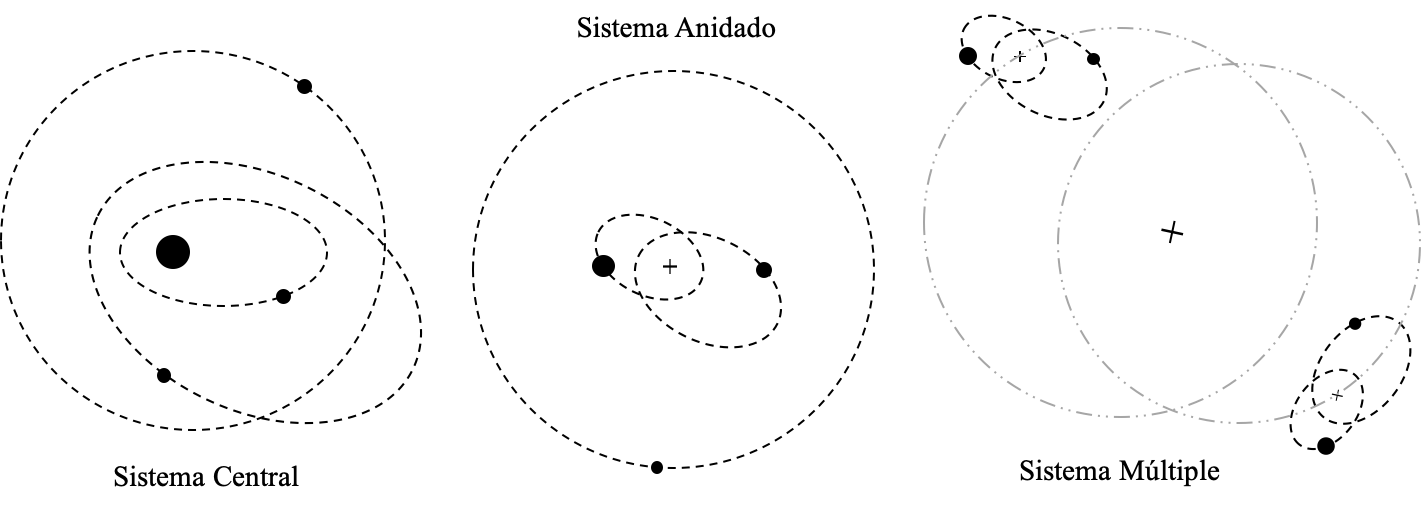
\includegraphics[width=1.0\textwidth]{./figures/horizontal_sistemas_jerarquicos.png}
\caption{Tipos de sistemas jerarquicos de N
cuerpos.\label{fig:sistemas_jerarquicos}}
\end{figure}

Resolver el problema de los dos cuerpos no es entonces, simplemente, una
manera burda de estudiar sistemas más complejos formados por muchos
cuerpos interactuantes. En sistemas jerárquicos el problema de dos
cuerpos, sumado a la teoría de perturbaciones, es la manera en la que
normalmente se estudia la dinámica de los sistemas.



\hypertarget{doscuerpos_reducido}{%
\section{El problema relativo de dos
cuerpos}\label{doscuerpos_reducido}}

Naturalmente el problema de dos cuerpos es un caso particular del
problema de los N cuerpos y la mayoría de las propiedades que
descubrimos en el \autoref{problema_ncuerpos} son válidas también en
este caso.

Las ecuaciones de movimiento del sistema se reducen a (Ecs.
\ref{eq:edm_ncuerpos}):

\begin{eqnarray}
\label{eq:edm_doscuerpos}
\ddot{\vec{r}}_1 & = & -\frac{\mu_2}{r_{12}^3}{\vec r}_{12} \\
\nonumber
\ddot{\vec{r}}_2 & = & -\frac{\mu_1}{r_{21}^3}{\vec r}_{21}
\end{eqnarray} donde
\({\vec r}_{12}={\vec r}_1-{\vec r_2}=-{\vec r}_{21}\) (ver
\autoref{fig:problema_dos_cuerpos}.)

Al reducirse de orden, las Ecs. (\ref{eq:edm_doscuerpos}) corresponden a
un total de 12 ecuaciones diferenciales ordinarias escalares de primer
orden, con incognitas \(x_1(t),y_1(t),z_1(t)\),
\({\dot x}_1(t),{\dot y}_1(t),{\dot z}_1(t)\) y
\(x_2(t),y_2(t),z_2(t)\), \({\dot x}_2(t),{\dot y}_2(t),{\dot z}_2(t)\).

\begin{figure}[t!]
\centering
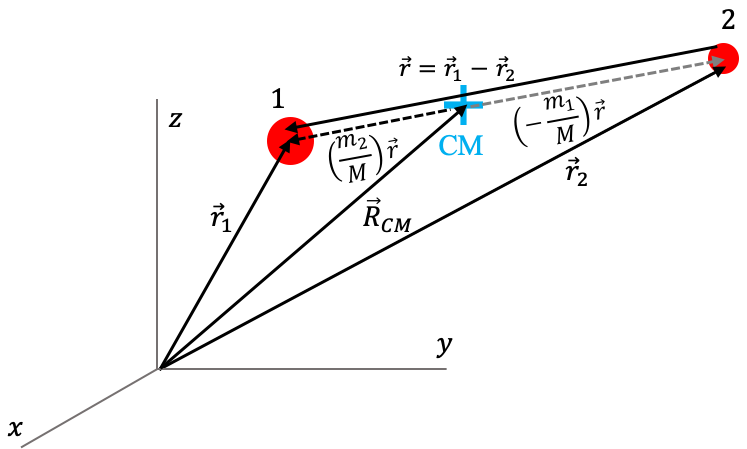
\includegraphics[width=0.8\textwidth]{./figures/horizontal_centro_masa.png}
\caption{Configuración del problema de los dos
cuerpos.\label{fig:problema_dos_cuerpos}}
\end{figure}

Las constantes de movimiento son las mismas que encontramos en la
\autoref{solucion_analitica}:

\begin{itemize}
\tightlist
\item
  Tres para el momento lineal del centro de masa, Ec.
  (\ref{eq:ncuerpos_momento}).
\item
  Tres para la posición inicial del centro de masa, Ec.
  (\ref{eq:ncuerpos_centro_masa}).
\item
  Tres para el momento angular total, Ec.
  (\ref{eq:ncuerpos_momento_angular})
\item
  Una para la energía mecánica total, Ec. (\ref{eq:ncuerpos_energia})
\end{itemize}

El problema tiene entonces, hasta ahora, tan solo 10 cuadraturas
(constantes de movimientos) que relacionan algebraicamente 12 variables
dependientes. Por lo tanto, si bien en esta caso el Teorema de Bruns
generalizado, Teo. (\ref{box:teo:bruns}) no limita la posibilidad de
encontrar otras constantes independientes, con la información
disponible, el problema no puede resolverse por cuadraturas.

Hay sin embargo dos ``simetrías'' que reducen considerablemente el
problema y nos ponen en el camino de una solución analítica completa.

La primera simetría la identificamos en la \autoref{centro_masa} y
esta ilustrada en la \autoref{fig:problema_doscuerpos}). Habíamos
mostrado que el centro de masa de un sistema de dos cuerpos esta siempre
ocalizado sobre la línea que une las dos partículas. Esto implica que la
posición de cada partícula puede expresarse como función de una sola
cantidad vectorial, a saber, el vector relativo
\({\vec r}\equiv{\vec r}_{12}\):

\begin{eqnarray}
\label{eq:r1_r2_r}
{\vec r}_1 & = & {\vec R}_\mathrm{CM}+\frac{m_2}{M} \vec r\\
\nonumber
{\vec r}_2 & = & {\vec R}_\mathrm{CM}-\frac{m_1}{M} \vec r
\end{eqnarray} y por consiguiente también la velocidad de las partículas
es función solamente de la velocidad relativa entre ellas:

\begin{eqnarray}
\label{eq:v1_v2_v}
\dot{\vec r}_1 & = & \vec{V}_\mathrm{CM}+\frac{m_2}{M} \dot{\vec r}\\
\nonumber
\dot{\vec r}_2 & = & \vec{V}_\mathrm{CM}-\frac{m_1}{M} \dot{\vec r}
\end{eqnarray}

Resolver el problema de los dos cuerpos consiste entonces, en realidad,
en encontrar las funciones \(\vec r(t)\) y \(\dot{\vec r}(t)\) que
describen el movimiento del vector relativo.

Para encontrar la e.d.m. del vector relativo, basta que restemos las
Ecs. (\ref{eq:edm_doscuerpos}) y tengamos en cuenta que, por definición,
\(\ddot{\vec{r}} = \ddot{\vec{r}}_2 - \ddot{\vec{r}}_1\):

\begin{equation}
\label{eq:edm_doscuerpos_relativo}
\ddot{\vec{r}}=-\frac{\mu}{r^3}\vec{r}
\end{equation} donde hemos introducido \(\mu \equiv G(m_1+m_2)\) que
llamaremos en lo sucesivo el \emph{parámetro gravitacional del sistema}.

Con esta simetría, hemos reducido el tamaño del problema de las 12
ecuaciones diferenciales ordinarias de primer orden equivalentes a las
Ecs. (\ref{eq:edm_doscuerpos}), a solo 6 ecuaciones (la versión reducida
de la Ec. \ref{eq:edm_doscuerpos_relativo}), al costo, sin embargo, de
abandonar las coordenadas originales y por la misma razón las
cuadraturas que encontramos anteriormente.

Si queremos obtener la solución a este problema por el método de
cuadraturas, debemos entonces encontrar 6 constantes de movimiento a
partir de la Ec. (\ref{eq:edm_doscuerpos_relativo}) y que relacionen las
6 variables del problema: \(x(t)\), \(y(t)\), \(z(t)\), \(v_x(t)\),
\(v_y(t)\), \(v_z(t)\).

\hypertarget{doscuerpos_constantes}{%
\section{Constantes de movimiento}\label{doscuerpos_constantes}}

Es claro que la Ec. (\ref{eq:edm_doscuerpos_relativo}), a diferencia de
lo que paso en el problema de los N cuerpos con la Ec.
(\ref{eq:ncuerpos_suma_edm}), no puede expresarse directamente en
cuadraturas sin la ayuda de un factor integrante. Esto implica que en el
problema relativo, a diferencia de lo que pasa en el problema de los N
cuerpos, el momento lineal no es constante.

\hypertarget{doscuerpos_h}{%
\subsection{Momento angular específico relativo}\label{doscuerpos_h}}

Si pre multiplicamos ambos lados de la Ec.
(\ref{eq:edm_doscuerpos_relativo}) por \(\vec r\times\) obtenemos:

\[
\vec r\times \ddot{\vec r}=0
\] que puede expresarse en cuadraturas como:

\[
\frac{\mathrm{d}}{\mathrm{d}t} (\vec{r}\times \dot{\vec{r}}) = 0
\] de donde encontramos nuestro primera constante de movimiento:

\begin{equation}
\label{eq:h}
\vec{r} \times \dot{\vec{r}}\equiv\vec{h}
\end{equation}

Si bien esta cantidad no se corresponde con ninguna cantidad dinámica
del sistema original, su estructura y unidades nos recuerda la
definición de un momento angular específico (momento angular por unidad
de masa) y en lo sucesivo llamaremos a \(\vec h\) el \emph{momento
angular específico relativo} del problema.

La constancia de la cantidad \(\vec r\times\dot{\vec r}\) tiene una
implicación mas trascendental aún. Como sucedió en el problema de los N
cuerpos con el momento angular total referido al centro de masa, el
vector constante \(\vec h\) define un plano invariable, el análogo aquí
del plano invariable de Laplace de la Def.
(\ref{box:def:plano.invariable}). Este plano, a diferencia del que
encontramos en el problema de los N cuerpos, tiene una propiedad
distintiva y crucial. Dado que por definición, el vector relativo
\(\vec r\) y su velocidad \(\dot{\vec r}\) son perpendiculares a
\(\vec h\), ambos residiran siempre sobre ese plano (ver
\autoref{fig:plano_orbital}). Como resultado, la trayectoria del vector
relativo se realizará siempre sobre un plano (que en el sistema de
referencia del centro de masa será invariable también.) Llamamos a este
plano, el \textbf{plano orbital} del sistema.

\begin{figure}[t!]
\centering
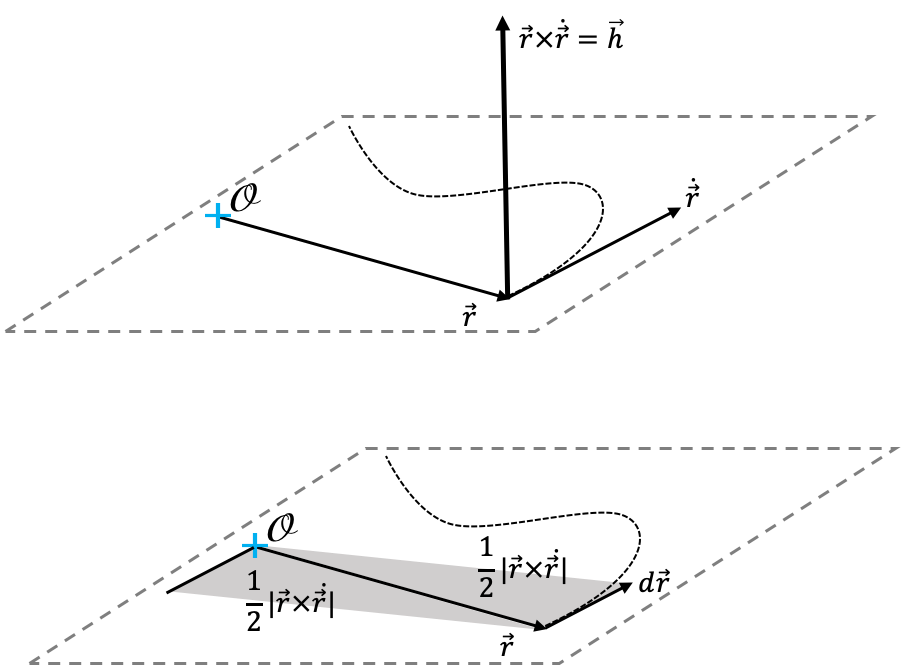
\includegraphics[width=0.8\textwidth]{./figures/square_plano_orbital.png}
\caption{El problema de los dos cuerpos puede reducirse al movimiento de
su vector relativo \(\vec r\), un vector libre sin un origen definido.
Por simplicidad podemos suponer la existencia un punto imaginario
\({\cal O}\) alrededor del cual la punta del vector se mueve. La
constancia de \(\vec r\times\dot{\vec r}=\vec h\) en el problema
relativo de los dos cuerpos implica que el movimiento del sistema
(trayectoria rayada) se realiza sobre un plano: aquel definido por el
vector \(\vec h\). Adicionalmente (panel inferior) la magnitud de este
vector se puede relacionar con la razón de cambio del área barrida por
el vector relativo (superficie coloreada en el panel
inferior.)\label{fig:problema_dos_cuerpos}}
\end{figure}

La existencia de un plano orbital en el problema relativo de los dos
cuerpos es una simetría nueva que reduce aún más el ``tamaño'' del
sistema. Ahora, podemos escribir explícitamente el vector posición y el
vector velocidad sobre el plano en términos de sus componentes en
coordenadas cilíndricas (ver la \autoref{sistemas_coordenadas}),
como:

\begin{eqnarray}
\label{eq:r}
\vec{r} & = & r\hat{a_r} \\
\label{eq:dotr}
\dot{\vec{r}} & = & \dot{r}\hat{a_r} + r\dot{\theta} \hat{a_\theta}
\end{eqnarray} y con esto el problema de los dos cuerpos relativo se
reduce a encontrar las cuatro funciones \(r(t)\), \(\theta(t)\),
\(\dot{r}(t)\) y \(\dot{\theta}(t)\) o sus equivalente cartesianos
\(x(t)\), \(y(t)\), \(\dot{x}(t)\) y \(\dot{y}(t)\).

En el plano orbital, el momento angular específico relativo tiene solo
una componente no nula (en dirección \(z\)) y se puede escribir
simplemente como \(\vec{h}:(0,0,h)\), donde de las Ecs. (\ref{eq:r}) y
(\ref{eq:dotr}),

\begin{equation}
\label{eq:h_escalar}
h=r^2\dot\theta
\end{equation}

La magnitud del vector \(\vec h\) tiene un significado adicional que
viene directamente de la interpretación geométrica de la magnitud del
producto cruz \(2\mathrm{dA}=|\vec r\times \mathrm{d}{\vec r}|\) que no
es otra cosa que el área del paralelogramo definido por los vectores
\(\vec r\) y \(\mathrm{d}{\vec r}\) (ver Figura
\autoref{fig:teorema_areas}.):

\[
h=2\frac{\mathrm{d}A}{\mathrm{d}t}
\]

La constancia \(h\) conduce a uno de los más conocidos teoremas de la
mecánica celeste:
\begin{box_theorem}{Proposición}{box:teo:areas}

\textbf{Teorema de áreas.} La \emph{velocidad areal} del vector relativo
(la razón de cambio del área barrida por el vector en su movimiento) en
el problema de los dos cuerpos es constante e igual a:

\begin{equation}
  \label{eq:velocidad_areal}
  \frac{\mathrm{d}A}{\mathrm{d}t}=\frac{1}{2}h
  \end{equation}

donde \(h=|\vec r\times\dot{\vec r}|\).

En otros términos, el vector relativo en el problema de los dos cuerpos
barre áreas iguales en tiempos iguales.

\end{box_theorem}
El teorema de áreas fue introducido originalmente en 1609 por Johanes
Kepler en su obra cumbre ``\emph{Astronomía Nueva}''. Kepler lo obtuvo
por inducción (a diferencia de como lo hicimos aquí por deducción a
partir de las ecuaciones de movimiento) con el objetivo específico de
describir de la forma más precisa posible el movimiento del planeta
Marte alrededor del Sol, del cual contaba con las observaciones precisas
realizadas durante varias decadas por el astrónomo danés Tycho Brahe
(\hreffoot{https://es.forvo.com/word/tycho_brahe/\#da}{``tico braja''})
Kepler, extendió este resultado ``empírico'' a todos los planetas, razón
por la cual se lo conoce históricamente como la \emph{segunda ley del
movimiento planetario}.

Hay dos diferencias importantes entre la segunda ley de Kepler y el
teorema de áreas formulado aquí. Mientras que la ley clásica aplica
únicamente para el movimiento de planetas en trayectorias cerradas
alrededor del Sol (que se asumía inmóvil) la versión moderna del teorema
no hace ninguna suposición específica sobre la forma (si es cerrada o
abierta) de la trayectoria del vector relativo. Adicionalmente, el
teorema de áreas no dice nada sobre la relación entre las masas y se
aplica universalmente a cualquier sistema de dos cuerpos, sea está la
descripción (aproximada) el movimiento de un planeta alrededor del Sol,
la de un cometa que sobrevuela a Júpiter o un sistema binario de
estrellas de neutrones con masas similares

Formulado en términos de la velocidad areal, el teorema de áreas es
relativamente oscuro. Si usamos la magnitud del vector \(\vec h\) (Ec.
\label{eq:h_escalar}) y escribimos:

\begin{equation}
\label{eq:dotq}
\dot\theta=\frac{h}{r^2}
\end{equation} otra manera de interpretar la constancia del momento
angular específico es decir que la velocidad angular \(\dot\theta\) del
vector relativo es mayor en tanto menor sea la magnitud el vector \(r\)
(distancia entre las partículas.) Es decir, las partículas del sistema
se mueven más rapidamente en los puntos de máxima aproximación que en
aquellos en los que están más lejos. Este comportamiento ya lo intuíamos
al observar la solución numérica de los sistemas que estudiamos en el
\autoref{problema_ncuerpos}.

\hypertarget{doscuerpos_epsilon}{%
\subsection{Energía específica relativa}\label{doscuerpos_epsilon}}

Si pre multiplicamos ambos lados de la Ec.
(\ref{eq:edm_doscuerpos_relativo}) por \(\vec r\cdot\) obtenemos:

\[
\dot{\vec{r}} \cdot \ddot{\vec{r}} = -\frac{\mu}{r^3} \dot{\vec{r}} \cdot \vec{r}\\
\] que puede expresarse en cuadraturas como:

\[
\frac{d}{dt} \left(\frac{1}{2} \dot{\vec{r}}^2 \right)= \frac{d}{dt}\left(\frac{\mu}{r}\right)
\] de donde encontramos una segunda constante de movimiento:

\begin{equation}
\label{eq:epsilon}
\frac{1}{2} \dot{\vec{r}}^2 - \frac{\mu}{r}\equiv\epsilon
\end{equation}

Si bien, como sucedió con \(\vec h\), esta cantidad no se corresponde
con ninguna cantidad dinámica del sistema original, su estructura y
unidades nos recuerda la definición de una energía mecánica específica
(energía mecánica por unidad de masa) y en lo sucesivo llamaremos a
\(\epsilon\) la \emph{energía específico relativa} del problema.

De nuevo, teniendo en cuenta que el movimiento se realiza sobre un
plano, la energía específica relativa se puede escribir en términos de
las componentes cartesianas en la forma:

\begin{equation}
\label{eq:epsilon_cartesianas}
\frac{1}{2}({\dot x}^2+{\dot y}^2)-\frac{\mu}{\sqrt{x^2+y^2}}=\epsilon,
\end{equation} o en coordenadas cilíndricas como:

\begin{equation}
\label{eq:epsilon_cilindricas}
\frac{1}{2}({\dot r}^2+r^2\dot{\theta}^2)-\frac{\mu}{r}=\epsilon
\end{equation} donde al poner \(\epsilon\) del lado derecho de la
ecuación estamos reafirmando simbólicamente el hecho de que la fórmula
del lado izquierdo es la que define explícitamente la cuadratura que
puede, eventualmente, conducirnos a una solución exacta del problema.
\(\epsilon\) no es más que un número cuyo valor puede calcularse usando
estas fórmulas por ejemplo a partir de las condiciones iniciales del
problema.

\bigskip

Hasta aquí hemos conseguido dos cuadraturas del problema:

\begin{itemize}
\tightlist
\item
  La magnitud del momento angular específico relativo, Ec.
  (\ref{eq:h_escalar}), cuyo valor es \(h\).
\item
  La energía específica relativa, Ec. (\ref{eq:epsilon_cilindricas}),
  cuyo valor es \(\epsilon\).
\end{itemize}

Si queremos resolver el problema por caudraturas necesitamos obtener
cuatro constantes, el número de variables dependientes del problema
relativo sobre el plano orbital. De acuerdo al Teorema de Bruns, para
sistema con 3 o más cuerpos no hay ninguna otra constante de movimiento
que sea independiente de las anteriores. En el problema relativo de los
dos cuerpos, sin embargo, existe una constante nueva que nos permite
resolver analíticamente el problema.

\hypertarget{doscuerpos_e}{%
\subsection{El vector de excentricidad}\label{doscuerpos_e}}

Que pasa si postmultiplicamos ambos lados de la Ec.
(\ref{eq:edm_doscuerpos_relativo}) por \(\times\vec h\):

\[
\ddot{\vec{r}}\times \vec{h} = -\frac{\mu}{r^3} \vec{r}\times \vec{h}
\]

Dado que \(\vec h\) es constante, el lado izquierdo se puede escribir en
cuadraturas:

\begin{equation}
\label{eq:edmxh}
\frac{\mathrm{d}}{\mathrm{d}t}(\dot{\vec{r}}\times \vec{h})=-\frac{\mu}{r^3} \vec{r}\times \vec{h}
\end{equation}

Por su parte en el lado derecho:

\[
\begin{array}{rcl}
\vec{r}\times \vec{h} & = & \vec{r} \times (\vec{r} \times \dot{\vec{r}})\\
& = & \vec{r}(\vec{r}\cdot \dot{\vec{r}}) - \dot{\vec{r}}( \vec{r} \cdot \vec{r})\\
& = & \vec{r}r\dot{r} - \dot{\vec{r}}r^2
\end{array}
\] que multiplicando por \(-\mu/r^3\) también se puede escribir en
cuadraturas como:

\begin{eqnarray}
\nonumber
\vec{r}\times \vec{h} & = & -\mu \left(\frac{\vec{r}\dot{r}}{r^2} - \frac{\dot{\vec{r}}}{r}\right)\\
\nonumber
& = & \frac{\mathrm{d}}{\mathrm{d}t}\left(\mu \frac{\vec{r}}{r} \right)
\end{eqnarray}

Con todo esto la Ec. (\ref{eq:edmxh}) en cuadraturas completas queda:

\begin{equation}
\label{eq:cuadratura_e}
\frac{\mathrm{d}}{\mathrm{d}t}(\dot{\vec{r}}\times \vec{h})=\frac{\mathrm{d}}{\mathrm{d}t}\left(\mu \frac{\vec{r}}{r} \right)
\end{equation}

y de aquí podemos identificar una nueva y complementamente independiente
constante de movimiento:

\begin{equation}
\label{eq:e}
\frac{\dot{\vec{r}} \times \vec{h}}{\mu} - \frac{\vec{r}}{r}\equiv\vec{e}
\end{equation}

La razón por la que hemos expresado esta integral dividiendo la
cuadratura en la Ec. (\ref{eq:cuadratura_e}) por \(\mu\) es para hacer a
la constante resultante adimensional (recordemos que \(\mu\) tiene
unidades de L\(^3\)/T\(^2\)) lo que es mas conveniente para su
manipulación numérica.

¿Cuál es el significado geométrico o físico del vector \(\vec e\)? A
diferencia de lo que pasó con \(\vec h\) y con \(\epsilon\), no es
trivial encontrar ahora una cantidad dinámica que podamos asociar con
\(\vec e\). Este vector, sin embargo ha aparecido en distintos contextos
en la historia de la física y las matemáticas, desde la mecánica celeste
misma, pasando por el cálculo vectorial hasta la más reciente mecánica
cuántica (ver recuadro \emph{Un poco de historia, Laplace, de la
mecánica celeste a la mecánica cuántica}.)

No es difícil mostrar que \(\vec e\) no es enteramente independiente de
\(\vec h\) y \(\epsilon\). Si se valcula la magnitud del vector se
obtiene la relación (ver problemas al final del capítulo):

\begin{equation}
\label{eq:e_h_epsilon}
e=\sqrt{1+\frac{2\epsilon h^2}{\mu^2}}
\end{equation} que será de gran utilidad en lo que queda de este
capítulo y en general en la mecánica celeste.

\hypertarget{doscuerpos_ecuacion}{%
\section{La ecuación de la trayectoria}\label{doscuerpos_ecuacion}}

Una manera de encontrar una interpretación geométrica para el vector
\(\vec e\) es comparar su dirección con la de otros vectores en el plano
orbital. Sabemos, por su definición en la Ec. (\ref{eq:e}) que
\(\vec e\) esta en el mismo plano que \(\vec r\) y \(\dot{\vec r}\). Si
proyectamos \(\vec e\) sobre el vector posición obtenemos:

\[
\vec{e}\cdot\vec{r} = \frac{1}{\mu}\vec{r} \cdot (\dot{\vec{r}} \times \vec{h}) 
- \vec{r}\cdot\frac{\vec r}{r}
\]

Utilizando la propiedad cíclica del tripe producto escalar (Ec.
\ref{eq:triple_producto_escalar}) el primer término del lado derecho de
la ecuación queda:

\[
\begin{array}{rcl}
\vec{r} \cdot (\dot{\vec{r}} \times \vec{h}) & = & \vec{h} \cdot (\vec{r} \times \dot{\vec{r}})\\
& = & \vec{h} \cdot \vec{h} \\
& = & h^2
\end{array}
\] de donde, la proyección es simplemente:

\[
\vec{e}\cdot\vec{r} = \frac{h^2}{\mu} - r
\]

Si ahora hacemos \({\vec e} \cdot {\vec r} = e r\cos \theta_{er}\), con
\(\theta_{er}\) el ángulo entre el vector \(\vec e\) y el vector
posición \(\vec r\) sobre el plano orbital, la proyección se puede
escribir como:

\[
e r\cos \theta_{er} = \frac{h^2}{\mu} - r
\] de la que podemos despejar explícitamente \(r\) en función de
\(\theta_{er}\):

\begin{equation}
\label{eq:doscuerpos_trayectoria}
r = \frac{h^2/\mu}{1 + e \cos \theta_{er}},
\end{equation} que es claramente la ecuación de una cónica con
\emph{semilatus rectum}, \(p=h^2/\mu\), excentricidad \(e=|\vec e|\) y
anomalía verdadera \(f=\theta_{er}\).

No solo hemos encontrado la interpretación geométrica para el vector
\(\vec e\) (el vector esta dirigido hacia el periapsis de la cónica y su
magnitud es la excentricidad de la misma) sino que además encontramos
con este sencillo procedimiento la forma general de la trayectoria
descrita por el vector relativo en el problema de los dos cuerpos. Este
resultado lo podemos formular como un teorema general:
\begin{box_theorem}{Proposición}{box:teo:movimiento.orbital}

\textbf{Primer teorema del movimiento orbital.} El extremo del vector
relativo en el problema de los dos cuerpos, describe en el plano orbital
una trayectoria cónica con foco en el origen imaginario \({\cal O}\)
(extremo del vector relativo), periapsis en la dirección del vector
\(\vec e=(\dot{\vec{r}} \times \vec{h})/{\mu} - {\vec r}/r\),
excentricidad igual a \(|\vec e|=\sqrt{1+2\epsilon h^2/\mu^2}\) y
semilatus rectum \(p=h^2/\mu\).

\end{box_theorem}
Este teorema es el equivalente moderno a la primera ley (empírica) de
Kepler del movimiento planetario, formulada al mismo tiempo con su
segunda ley (ver Teo. \ref{box:teo:area}) en 1609 en su texto
``\emph{Astronomía nueva}''. A diferencia de la deducción realizada
aquí, Kepler, después de estudiar el movimiento de Marte, esencialmente
adivinó que su trayectoria debía ser una elipse. Adicionalmente y a
diferencia de la primera ley de Kepler, el primer teorema del movimiento
orbital formulado aquí no se restringe al caso de trayectorias
elípticas, para las cuáles \(|\vec e|<1\), sino que en principio predice
que la trayectoria del vector relativo podría ser cualquier cónica
incluyendo también una línea recta, una parábola o una hipérbola.
\begin{box_history}{Un poco de historia}{}{nofloat}
\small

\textbf{Laplace y el vector de excentricidad.} Aunque pensamos
normalmente que la solución al problema de los dos cuerpos fue obtenida
por primera vez por Newton, en realidad la versión desarrollada aquí no
es precisamente la que apareció en los \emph{Principia}.

El primero en seguir el procedimiento y la notación mostrada aquí,
usando para ello las constantes de movimiento en el problema, y en
particular el vector de excentricidad, fue el científico estadoudinense
\textbf{Josiah Willard Gibbs} (1839-1903.) Gibbs es además el padre de
la notación vectorial que hemos usado y usaremos a lo largo de este
texto, por lo que muchos de los resultados presentados aquí no tuvieron
esta forma antes de 1870 cuando Gibbs escribió sus trabajos en el tema.

Gibbs había a su vez tomado la idea del vector de excentricidad de los
trabajos del matemático alemám \textbf{William Rowan Hamilton}. En 1845,
Hamilton publicó un artículo titulado ``Aplicaciones de los cuaterniones
en algunos problemas dinámicos'' (los cuaterniones fueron inventados por
Hamilton y precedieron a los vectores geométricos de Gibbs.) En este
trabajo, el matemático alemán reportaba el descubrimiento de una nueva
constante de movimiento en el problema de los dos cuerpos, precisamente
el vector \(\vec e\) de la Ec. (\ref{eq:e}).

Hoy sabemos que en realidad, Hamilton no había descubierto nada nuevo.
La primera referencia conocida del vector de excentricidad se debe al
matemático Francés Pierre-Simon Laplace \cite{Goldstein1975LRL1}. Es por
esto que hoy al vector \(\vec e\) (o en realidad versiones analogas al
mismo) se lo conozca en algunos contextos como el \emph{vector de
Laplace}. Para ser justos deberíamos llamarlo el \emph{vector de
Laplace-Hamilton}. Si bien Laplace no uso exactamente la notación y el
procedimiento mostrado en esta sección, es un hecho conocido que dedujo
la forma que debía tener la órbita en el problema reducido de los dos
cuerpos, manipulando el vector \(\vec e\) de manera analoga a como lo
hicimos aquí.

Laplace (1749-1827, ver \autoref{fig:laplace}) es una de las figuras más
sobresalientes de las matemáticas, la física, la ingeniería y la
astronomía de los 1700 y principios de los 1800. Los principios y
problemas básicos de la mecánica celeste que fueron presentados y
desarrollados por Newton y sus contemporáneos en términos geométricos,
fueron traducidos enteramente en términos de cálculo infinitesimal
(incluyendo la teoría de ecuaciones diferenciales) por Laplace, quién
presentó a partir de 1799 una síntesis de todos los avances en el área
que se habían realizado en los más de 100 que habían transcurrido desde
la publicación de los \emph{Principia} en 1687. El resultado fue un
tratado de cinco volumenes titulado convenientemente \emph{Traité de
mécanique céleste} (Tratado de Mecánica Celeste o abreviado la Mecánica
Celeste.)

La Mecánica Celeste de Laplace es considerado por muchos el libro más
importante en el área escrito después de los \emph{Principia}. Allí,
además de la solución original al problema de los dos cuerpos presentada
en esta sección, Laplace abordó la mayoría de los problemas centrales de
la mecánica celeste, incluyendo algunos que Newton no había podido
resolver: la teoría general de perturbaciones, la teoría general de
mareas gravitacionales, el movimiento en campos gravitacionales
producidos por cuerpos no esféricos, la estabilidad del sistema solar,
entre muchos otros.

Muchos de los resultados en este libro y en la mayoría de los textos de
mecánica celeste escritos en los últimos 200 años, son en realidad
reelaboraciones modernas o aplicaciones de los resultados presentados en
la Mecánica Celeste de Laplace.

\end{box_history}
\begin{figure}[t!]
\centering
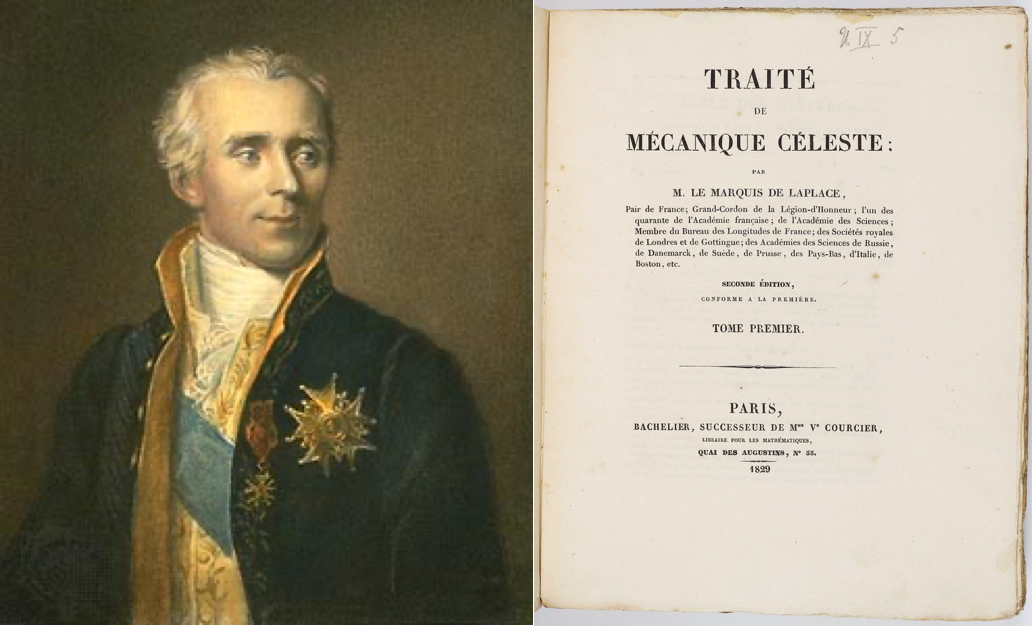
\includegraphics[width=1.0\textwidth]{./figures/horizontal_laplace.png}
\caption{Izquierda: pintura de Pierre-Simon Laplace de James
Posselwhite. Derecha: portada del Tomo I del Tratado de Mecánica Celeste
de Laplace, el libro más importante en el área publicado después de los
\emph{Principia} (foto Colección \emph{Heralds of Science from the
Burndy Library}.)\label{fig:laplace}}
\end{figure}

Una cosa es el movimiento del vector relativo y otra la trayectoria que
describen las partículas mismas en el espacio ¿son también esas
trayectorias cónicas?

Usando las Ecs. (\ref{eq:r1_r2_r}) y la solución en la Ec.
(\ref{eq:doscuerpos_trayectoria}) puede probarse que la distancia de
cada partícula al centro de masa esta dada por:

\begin{eqnarray}
\label{eq:doscuerpos_trayectoria_m1}
r_1 & = & \frac{(m_2/M) h^2/\mu}{1 + e \cos f }\\
\label{eq:doscuerpos_trayectoria_m2}
r_2 & = & \frac{(m_1/M) h^2/\mu}{1 + e \cos f }\\
\end{eqnarray}

Este resultado implica las dos partículas tienen trayectorias cónicas
con idéntica excentricidad, foco en el centro de masa y \emph{semilatus
rectum} proporcional a la distancia de cada una al centro de masa:

\begin{eqnarray}
\nonumber
p_1 & = & \frac{m_2}{M}p\\
p_2 & = & \frac{m_1}{M}p\\
\end{eqnarray}

En la \autoref{fig:doscuerpos_trayectorias} mostramos un ejemplo de la
trayectoria elíptica del vector relativo y las trayectorias
correspondientes de las dos partículas.

\begin{figure}[t!]
\centering
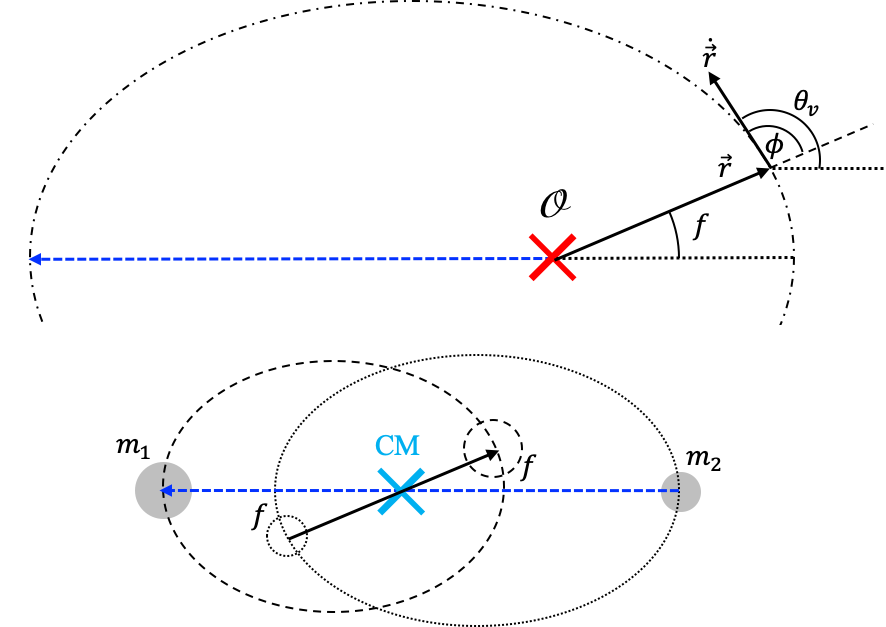
\includegraphics[width=1.0\textwidth]{./figures/horizontal_doscuerpos.png}
\caption{Trayectorias del vector relativo (arriba) y de las partículas
individuales (abajo). Las trayectorias tienen todas la misma
excentricidad. El foco de la trayectoria del vector relativo es un punto
arbitrario en el espacio \(\cal O\), mientras que el foco de las
trayectorias de las partículas es el centro de masa (CMD). El vector
relativo se muestra en dos posiciónes: en el apoapsis (flecha rayada) y
en un punto cualquiera de la trayectoria (flecha continua.) Nótese que
la anomalía verdadera \(f\) es igual en las tres
trayectorias.\label{fig:doscuerpos_trayectorias}}
\end{figure}

\hypertarget{doscuerpos_velocidad}{%
\section{La velocidad relativa}\label{doscuerpos_velocidad}}

En la sección anterior mostramos que es posible, sin resolver el
problema relativo de los dos cuerpos (es decir sin encontrar expresiones
para la posición y velocidad relativa como función del tiempo), usar una
de las cuadraturas (el vector de excentricidad) para escribir la
ecuación en coordenadas cilíndricas de la trayectoria (Ec.
\ref{eq:doscuerpos_trayectoria}.) Usando esa ecuación podemos encontrar
el vector posición \(\vec r:(r,\theta)\) para cualquier valor de
\(\theta\).

Ahora bien, ¿podemos, de forma análoga, saber cuál es el vector
velocidad \(\dot{\vec r}:(\dot r,r\dot \theta)\)?

La magnitud del vector velocidad (rapidez) esta contenida en la energía
específica relativa:

\[
\frac{v^2}{2}-\frac{\mu}{r}=\epsilon,
\] de modo que si sabemos \(\epsilon\) y \(r\) (esté último se puede
obtener con la Ec. \ref{eq:ncuerpos_trayectoria}) podemos obtener \(v\).

De otro lado es posible, usando esta cuadratura escribir una expresión
general para \(\epsilon\) que será de mucha utilidad en lo sucesivo.

Para ello partimos de reconocer que podemos, para calcular el valor de
la energía específica relativa, usar cualquier punto sobre la
trayectoria. En particular, en el periapsis donde \(r=q=a(1-e)\) (con
\(e\neq 1\)) y \(h=qv\), es decir \(v=h/q\):

\[
\epsilon=\frac{h^2}{2a^2(1-e)^2}-\frac{\mu}{a(1-e)}
\]

Después de una sencilla manipulación algebraica obtenemos:

\begin{equation}
\label{eq:e_mu_2a}
\epsilon=-\frac{\mu}{2a}
\end{equation}

Esta expresión es válida únicamente en el caso en el que \(e\neq 1\). En
el caso de la parábola, \(e=1\) puede mostrarse que \(\epsilon=0\).

Si reemplazamos en la cuadratura de la energía específica relativa (Ec.
\ref{eq:epsilon}) obtenemos:

\begin{equation}
\label{eq:vis_viva}
v^2=\mu\left(\frac{2}{r}-\frac{1}{a}\right)
\end{equation}

Donde de nuevo esta relación es válida únicamente si \(e\neq 1\).
Llamamos a esta relación la \emph{vis viva}.

Una interesante propiedad de la \emph{vis viva} es que dada una
distancia relativa inicial \(r\) y una rapidez relativa \(v\), el valor
del semieje mayor de la órbita resultante será independiente de la
dirección de la velocidad:

\[
a=\frac{\mu}{2\mu/r-v^2}
\]

La \emph{vis viva} nos permite calcular la magnitud de la velocidad,
pero ¿cuál es la dirección de \(\vec v\)?

Podemos usar para ello el vector \(\vec h\), cuya magnitud podemos
escribir como:

\[
h=|\vec r\times \dot{\vec r}|=vr\sin\phi
\] donde \(\phi\) es el ángulo entre el vector posición y la velocidad
(ver \autoref{fig:doscuerpos_trayectorias}) que llamaremos en lo
sucesivo el \emph{argumento de la velocidad} y que en virtud de la
expresión anterior esta dado por:

\begin{equation}
\label{eq:fi_conica}
\sin\phi=\frac{h}{rv}
\end{equation}
\begin{box_note}{Nota}

\textbf{Ángulo a partir de la magnitud del producto cruz.} Aunque la Ec.
(\ref{eq:fi_conica}) no tiene nunguna discusión, en la práctica el
cálculo de \(\phi\) a partir de ella tiene una sutileza. Dado que
\(h,r,v>0\) el signo de \(\sin\phi\) siempre será positivo. Eso
implicaría que \(\phi<\pi/2\). Sin embargo si calculamos ahora el
producto punto de \(\vec r\) y \(\dot{\vec r}\) (usando su definición en
coordenadas cilíndricas, \autoref{cantidades_cinematicas}):

\[
  cos\phi=\vec r\cdot\dot{\vec r}=r\dot{r}
  \]

De aquí vemos que cuando \(\dot{r}<0\), \(\cos\phi<0\) y por tanto
\(\phi>\pi/2\). Es decir la Ec. (\ref{eq:fi_conica}) solo nos dará el
valor correcto de \(\phi\) cuando \(\dot{r}\geq0\).

Pero, en términos de \(r\) y \(v\) ¿a qué condición corresponde
\(\dot{r}<0\)?

Sabemos que cuando \(0<f<\pi\), el vector relativo se estará alejando
del periapsis, es decir \({\dot r}>0\). Del otro lado cuando
\(\pi<f<2\pi\) entonces \({\dot r}<0\). De aquí podemos deducir una
fórmula, que si bien no es enteramente trivial, es lo mejor que podemos
hacer para calcular el argumento de la velocidad en el cuadrante
correcto:

\begin{equation}
  \phi = 
  \left\{
  \begin{array}{ll}
  \sin^{-1}\left(\frac{h}{rv}\right) & \mathrm{Si}\;0\leq f<pi\\
  \pi-\sin^{-1}\left(\frac{h}{rv}\right) & \mathrm{Si}\;\pi\leq f<2pi\\
  \end{array}
  \right.
  \end{equation}

\end{box_note}
Finalmente, el ángulo que forma la velocidad respecto a la dirección del
periapsis (dirección del vector \(\vec e\)) estará dada por:

\begin{equation}
\label{eq:tetav_conica}
\theta_v = f+\phi
\end{equation}

\hypertarget{hodografo_doscuerpos}{%
\section{El hodográfo del problema de los dos
cuerpos}\label{hodografo_doscuerpos}}

Hay una propiedad interesante que tiene el problema de los dos cuerpos.
Fue descubierta por Hamilton (ver recuadro \emph{Un poco de historia})
mientras estudiaba las consecuencias de describir el problema en
términos vectoriales (en realidad usando cuaterniones, los antepasados
de los vectores geométricos.)

Para conocer esta propiedad escribamos un algoritmo que nos permita
calcular las componentes del vector veclocidad a lo largo de la
trayectoria elíptica de un sistema de dos cuerpos ligado.

Supongamos para ello condiciones que nos garanticen que la cónica tiene
periapsis sobre el semieje \(x+\) (es decir \(\vec e/e={\hat e}_x\)). Si
asumimos condiciones iniciales del tipo \(\vec r_0=x_0{\hat e}_x\),
\(\dot{\vec r}_0=v_{0y}{\hat e}_y\), puede mostrarse que la condición
anterior se cumple si \(v_{0y}<\sqrt{\mu x_0}\) (ver problemas al final
del capítulo.)

Un conjunto de condiciones iniciales que cumple esta condición es:

    \begin{code}{}{}\begin{Verbatim}[fontsize=\small,commandchars=\\\{\}]
\PY{c+c1}{\PYZsh{}Condiciones iniciales}
\PY{n}{mu}\PY{o}{=}\PY{l+m+mi}{1} \PY{c+c1}{\PYZsh{}unidades canónicas (u.c.)}
\PY{k+kn}{from} \PY{n+nn}{numpy} \PY{k}{import} \PY{n}{array}
\PY{n}{x0}\PY{o}{=}\PY{l+m+mf}{1.0} \PY{c+c1}{\PYZsh{}u.c.}
\PY{n}{vy0}\PY{o}{=}\PY{l+m+mf}{0.5} \PY{c+c1}{\PYZsh{}u.c.}

\PY{c+c1}{\PYZsh{}Magnitud de h}
\PY{n}{h}\PY{o}{=}\PY{n}{x0}\PY{o}{*}\PY{n}{vy0}

\PY{c+c1}{\PYZsh{}Energía específica relativa}
\PY{k+kn}{from} \PY{n+nn}{numpy}\PY{n+nn}{.}\PY{n+nn}{linalg} \PY{k}{import} \PY{n}{norm}
\PY{n}{epsilon}\PY{o}{=}\PY{l+m+mf}{0.5}\PY{o}{*}\PY{n}{vy0}\PY{o}{*}\PY{o}{*}\PY{l+m+mi}{2}\PY{o}{\PYZhy{}}\PY{n}{mu}\PY{o}{/}\PY{n}{x0}
\end{Verbatim}

%%

\end{code}
\vspace{-1em}

%%hidecode


    \begin{Verbatim}[fontsize=\small,commandchars=\\\{\}]
h = 0.5
epsilon = -0.875
\end{Verbatim}

Usando las Ecs. (\ref{eq:doscuerpos_trayectoria}) y (\ref{eq:e}) podemos
calcular las propiedades de la órbita descrita por el vector relativo:

    \begin{code}{}{}\begin{Verbatim}[fontsize=\small,commandchars=\\\{\}]
\PY{c+c1}{\PYZsh{}Parámetros geométricos derivados}
\PY{k+kn}{from} \PY{n+nn}{numpy} \PY{k}{import} \PY{n}{sqrt}
\PY{n}{p}\PY{o}{=}\PY{n}{h}\PY{o}{*}\PY{o}{*}\PY{l+m+mi}{2}\PY{o}{/}\PY{n}{mu}
\PY{n}{e}\PY{o}{=}\PY{n}{sqrt}\PY{p}{(}\PY{l+m+mi}{1}\PY{o}{+}\PY{l+m+mi}{2}\PY{o}{*}\PY{n}{epsilon}\PY{o}{*}\PY{n}{h}\PY{o}{*}\PY{o}{*}\PY{l+m+mi}{2}\PY{o}{/}\PY{n}{mu}\PY{p}{)}
\PY{n}{a}\PY{o}{=}\PY{n}{p}\PY{o}{/}\PY{p}{(}\PY{l+m+mi}{1}\PY{o}{\PYZhy{}}\PY{n}{e}\PY{o}{*}\PY{o}{*}\PY{l+m+mi}{2}\PY{p}{)}
\end{Verbatim}

%%

\end{code}
\vspace{-1em}

%%hidecode


    \begin{Verbatim}[fontsize=\small,commandchars=\\\{\}]
p = 0.25
a = 0.5714285714285714
e = 0.75
\end{Verbatim}

Comprobamos que efectivamente para las condiciones iniciales provistas
la órbita resultante es una órbita elíptica (\(e<1\).)

Calculemos ahora las componentes de la velocidad de la partícula a lo
largo de la trayectoria, usando para ello la \emph{vis viva} (Ec.
\ref{eq:vis_viva}) y el argumento de la velocidad (Ecs.
\ref{eq:fi_conica} y \ref{eq:tetav_conica}):

    \begin{code}{}{}\begin{Verbatim}[fontsize=\small,commandchars=\\\{\}]
\PY{c+c1}{\PYZsh{}Valores de la anomalía verdadera}
\PY{k+kn}{from} \PY{n+nn}{numpy} \PY{k}{import} \PY{n}{linspace}\PY{p}{,}\PY{n}{pi}
\PY{n}{fs}\PY{o}{=}\PY{n}{linspace}\PY{p}{(}\PY{l+m+mi}{0}\PY{p}{,}\PY{l+m+mi}{2}\PY{o}{*}\PY{n}{pi}\PY{p}{,}\PY{l+m+mi}{100}\PY{p}{)}

\PY{c+c1}{\PYZsh{}Valores de r}
\PY{k+kn}{from} \PY{n+nn}{numpy} \PY{k}{import} \PY{n}{sin}\PY{p}{,}\PY{n}{cos}
\PY{n}{rs}\PY{o}{=}\PY{n}{p}\PY{o}{/}\PY{p}{(}\PY{l+m+mi}{1}\PY{o}{+}\PY{n}{e}\PY{o}{*}\PY{n}{cos}\PY{p}{(}\PY{n}{fs}\PY{p}{)}\PY{p}{)}

\PY{c+c1}{\PYZsh{}Valores de v}
\PY{n}{vs}\PY{o}{=}\PY{n}{sqrt}\PY{p}{(}\PY{n}{mu}\PY{o}{*}\PY{p}{(}\PY{l+m+mi}{2}\PY{o}{/}\PY{n}{rs}\PY{o}{\PYZhy{}}\PY{l+m+mi}{1}\PY{o}{/}\PY{n}{a}\PY{p}{)}\PY{p}{)}

\PY{c+c1}{\PYZsh{}Valores de phi}
\PY{k+kn}{from} \PY{n+nn}{numpy} \PY{k}{import} \PY{n}{arcsin}\PY{p}{,}\PY{n}{zeros\PYZus{}like}
\PY{n}{phis}\PY{o}{=}\PY{n}{zeros\PYZus{}like}\PY{p}{(}\PY{n}{fs}\PY{p}{)}
\PY{k}{for} \PY{n}{i}\PY{p}{,}\PY{n}{f} \PY{o+ow}{in} \PY{n+nb}{enumerate}\PY{p}{(}\PY{n}{fs}\PY{p}{)}\PY{p}{:}
    \PY{k}{if} \PY{n}{f}\PY{o}{\PYZlt{}}\PY{n}{pi}\PY{p}{:}
        \PY{n}{phis}\PY{p}{[}\PY{n}{i}\PY{p}{]}\PY{o}{=}\PY{n}{arcsin}\PY{p}{(}\PY{n}{h}\PY{o}{/}\PY{p}{(}\PY{n}{rs}\PY{p}{[}\PY{n}{i}\PY{p}{]}\PY{o}{*}\PY{n}{vs}\PY{p}{[}\PY{n}{i}\PY{p}{]}\PY{p}{)}\PY{p}{)}
    \PY{k}{else}\PY{p}{:}
        \PY{n}{phis}\PY{p}{[}\PY{n}{i}\PY{p}{]}\PY{o}{=}\PY{n}{pi}\PY{o}{\PYZhy{}}\PY{n}{arcsin}\PY{p}{(}\PY{n}{h}\PY{o}{/}\PY{p}{(}\PY{n}{rs}\PY{p}{[}\PY{n}{i}\PY{p}{]}\PY{o}{*}\PY{n}{vs}\PY{p}{[}\PY{n}{i}\PY{p}{]}\PY{p}{)}\PY{p}{)}

\PY{c+c1}{\PYZsh{}Valores de tetav}
\PY{k+kn}{from} \PY{n+nn}{numpy} \PY{k}{import} \PY{n}{mod}
\PY{n}{tetavs}\PY{o}{=}\PY{n}{phis}\PY{o}{+}\PY{n}{fs}

\PY{c+c1}{\PYZsh{}Componentes de la velocidad}
\PY{k+kn}{from} \PY{n+nn}{numpy} \PY{k}{import} \PY{n}{sin}
\PY{n}{vxs}\PY{o}{=}\PY{n}{vs}\PY{o}{*}\PY{n}{cos}\PY{p}{(}\PY{n}{tetavs}\PY{p}{)}
\PY{n}{vys}\PY{o}{=}\PY{n}{vs}\PY{o}{*}\PY{n}{sin}\PY{p}{(}\PY{n}{tetavs}\PY{p}{)}
\end{Verbatim}

%%

\end{code}

Hagamos una gráfica del extremo de la velocidad relativa:
%%HIDE%%
    \begin{code}{Algoritmo}{code:7_Problema2Cuerpos_20}\begin{Verbatim}[fontsize=\small,commandchars=\\\{\}]
\PY{k+kn}{import} \PY{n+nn}{matplotlib}\PY{n+nn}{.}\PY{n+nn}{pyplot} \PY{k}{as} \PY{n+nn}{plt}
\PY{n}{fig}\PY{o}{=}\PY{n}{plt}\PY{o}{.}\PY{n}{figure}\PY{p}{(}\PY{p}{)}
\PY{n}{ax}\PY{o}{=}\PY{n}{fig}\PY{o}{.}\PY{n}{gca}\PY{p}{(}\PY{p}{)}

\PY{c+c1}{\PYZsh{}Grafica}
\PY{n}{ax}\PY{o}{.}\PY{n}{plot}\PY{p}{(}\PY{n}{vxs}\PY{p}{,}\PY{n}{vys}\PY{p}{,}\PY{l+s+s1}{\PYZsq{}}\PY{l+s+s1}{r}\PY{l+s+s1}{\PYZsq{}}\PY{p}{)}

\PY{c+c1}{\PYZsh{}Decoración}
\PY{k+kn}{from} \PY{n+nn}{pymcel}\PY{n+nn}{.}\PY{n+nn}{plot} \PY{k}{import} \PY{n}{fija\PYZus{}ejes\PYZus{}proporcionales}
\PY{n}{valores}\PY{o}{=}\PY{p}{(}\PY{n}{vxs}\PY{p}{,}\PY{n}{vys}\PY{p}{)}
\PY{n}{xrango}\PY{p}{,}\PY{n}{yrango}\PY{o}{=}\PY{n}{fija\PYZus{}ejes\PYZus{}proporcionales}\PY{p}{(}\PY{n}{ax}\PY{p}{,}\PY{n}{valores}\PY{p}{,}\PY{n}{xcm}\PY{o}{=}\PY{l+m+mi}{0}\PY{p}{)}

\PY{c+c1}{\PYZsh{}Dibuja ejes}
\PY{n}{ax}\PY{o}{.}\PY{n}{plot}\PY{p}{(}\PY{n}{xrango}\PY{p}{,}\PY{p}{[}\PY{l+m+mi}{0}\PY{p}{,}\PY{l+m+mi}{0}\PY{p}{]}\PY{p}{,}\PY{l+s+s1}{\PYZsq{}}\PY{l+s+s1}{k\PYZhy{}}\PY{l+s+s1}{\PYZsq{}}\PY{p}{)}\PY{p}{;}
\PY{n}{ax}\PY{o}{.}\PY{n}{plot}\PY{p}{(}\PY{p}{[}\PY{l+m+mi}{0}\PY{p}{,}\PY{l+m+mi}{0}\PY{p}{]}\PY{p}{,}\PY{n}{yrango}\PY{p}{,}\PY{l+s+s1}{\PYZsq{}}\PY{l+s+s1}{k\PYZhy{}}\PY{l+s+s1}{\PYZsq{}}\PY{p}{)}\PY{p}{;}
\PY{n}{ax}\PY{o}{.}\PY{n}{set\PYZus{}xlabel}\PY{p}{(}\PY{l+s+s2}{\PYZdq{}}\PY{l+s+s2}{\PYZdl{}v\PYZus{}x\PYZdl{}}\PY{l+s+s2}{\PYZdq{}}\PY{p}{)}\PY{p}{;}
\PY{n}{ax}\PY{o}{.}\PY{n}{set\PYZus{}ylabel}\PY{p}{(}\PY{l+s+s2}{\PYZdq{}}\PY{l+s+s2}{\PYZdl{}v\PYZus{}y\PYZdl{}}\PY{l+s+s2}{\PYZdq{}}\PY{p}{)}\PY{p}{;}
\end{Verbatim}

%%

\tcblower
\footnotesize
\em ver Figura \ref{fig:code:7_Problema2Cuerpos_20}
\end{code}

    \begin{center}

\begin{figure}[ht!]
\centering
    \adjustimage{max size={0.8\linewidth}{0.8\paperheight}}{combined_files/combined_1242_0.png}
\caption{Figura correspondiente al código \ref{code:7_Problema2Cuerpos_20}.\label{fig:code:7_Problema2Cuerpos_20}}
\end{figure}

    \end{center}
%{ \hspace*{\fill} \\}
    
A este gráfico se lo conoce en general como el \emph{hodografo}. Como
podemos apreciar, en el problema de los dos cuerpos el hodógrafo es una
circunferencia descentrada, un resultado general que se puede formular
como un teorema general (cuya demostración puede desarrollarse en la
sección de problemas al final de este capítulo):
\begin{box_theorem}{Proposición}{box:teo:hodografo}

\textbf{El teorema del hodografo.} El vector velocidad relativa en el
problema de los dos cuerpos describe un círculo (hodografo) que tiene
centro en \((0,\mu e/h)\) y radio \(\mu/h\). Por la misma razón la
ecuación paramétrica para la velocidad es:

\begin{equation}
  \label{eq:v_hodografo}
  \begin{array}{rcl}
  \dot x & = & -\frac{\mu}{h} \sin f\\
  \dot y & = & \frac{\mu}{h} (e+\cos f)\\
  \dot z & = & 0\\
  \end{array}
  \end{equation}

Este resultado es independiente de la cónica (independiente del valor de
\(e\)).

\end{box_theorem}
\hypertarget{teorema_armuxf3nico}{%
\section{El teorema armónico}\label{teorema_armuxf3nico}}

En las secciones anteriores hemos usado las constantes de movimiento
para deducir dos importantes teoremas sobre del problema relativo de los
dos cuerpos que fueron descubiertas originalmente por Kepler y que se
conocen históricamente como las leyes del movimiento planetario.

En 1619, Kepler publicó su libro ``\emph{La armonía de los mundos}'' y
en el revelo la que sería una de las más increíbles leyes del movimiento
planetario (al menos para la época): la ley armónica. ¿Cuál es en
términos modernos el teorema que corresponde a esta ley?
\begin{box_theorem}{Proposición}{box:teo:armonico}

\textbf{Teorema armónico.} Dado un sistema de dos cuerpos cuyo
movimiento relativo es tal que \(e\neq 1\), la velocidad angular
promedio \(n=\langle\dot\theta\rangle\) del vector relativo es
independiente de la excentricidad de la órbita, y se relaciona con el
valor absoluto del semieje mayor de la órbita relativa \(|a|\) a través:

\begin{equation}\label{eq:teorema_armonico}n^2|a|^3 = \mu\end{equation}

\end{box_theorem}
Naturalmente esta no es la forma tradicional en la que conocemos la
tercera ley de Kepler. Esta última fue formulada solo en el caso de
movimiento sobre una órbita elíptica, mientras que el teorema general
formulado arriba aplica también en el caso de órbitas hiperbólicas.

En realidad la ley armónica es un corolario del teorema de áreas. En el
caso, por ejemplo, de una órbita elíptica, que es una órbita con período
\(T\), la velocidad areal se puede escribir como:

\[
\frac{\mathrm{d}A}{\mathrm{d}t}=\frac{A}{T}=\frac{\pi a b}{T}
\] donde hemos aprovechado el hecho que la velocidad areal es constante
para escribirla como la razón entre el área total de la elipse
\(A=\pi a b\) (Ec. \ref{eq:area_elipse}) y el período de la misma.

Si tenemos ahora en cuenta que \(b=a\sqrt{1-e^2}\), \(h^2=\mu a(1-e^2)\)
y \(\mathrm{d}A/\mathrm{d}t=h/2\) es fácil deducir que:

\begin{equation}
\label{eq:ley_armonica}
\frac{a^3}{T^2} = \frac{\mu}{4\pi^2}
\end{equation} que es la forma original de la ley armónica de Kepler:
``\emph{la razón entre el cubo del semiejemayor y el cuadrado del
período orbital de los planetas es constante}''.

Lo que no sabía Kepler era la relación de esa constante con constantes
física (la masa total del sistema) y geométricas (el factor \(4\pi^2\).)

Para obtener a partir de la Ec. (\ref{eq:ley_armonica}) la relación
entre \(a\) y \(n\) en el teorema armónico (Teo.
\ref{box:teo:armonico}), basta reconocer, de un lado, que en una órbita
periódica la velocidad angular promedio es:

\[
n=\frac{2\pi}{T}
\] y escribir la Ec. (\ref{eq:ley_armonica}) en la forma:

\[
a^3\left(\frac{2\pi}{T}\right)^2 = \mu
\]

Esta última es exactamente la relación \(n^2a^3=\mu\) del teorema
armónico.

En los problemas al final del capítulo el lector podrá demostrar el
teorema armónico en el caso de una órbita hiperbólica.

\hypertarget{teoremas_orbital}{%
\section{Teoremas del movimiento orbital}\label{teoremas_orbital}}

Podemos finalmente sintetizar los resultados de esta sección enumerando
en un mismo lugar los teoremas fundamentales del movimiento relativo de
dos cuerpos:

\begin{itemize}
\item
  \textbf{Primer teorema del movimiento orbital} (Teo.
  \ref{box:teo:movimiento.orbital}). El vector relativo de un sistema de
  dos cuerpos describe una trayectoria cónica.
\item
  \textbf{Teorema de áreas} (Teo. \ref{box:teo:areas}). La tasa de
  cambio del área barrida por el vector relativo es constante.
\item
  \textbf{Teorema armónico} (Teo. \ref{box:teo:armonico}). El producto
  del cuadrado de la velocidad angular promedio del vector relativo y el
  cubo del valor absoluto del semiejemayor de su trayectoria es
  constante.
\end{itemize}

Hoy, por su importancia histórica, estos teoremas son todavía conocidos
como las leyes del movimiento planetario de Kepler. Sin embargo, entre
las versiones originales de las leyes formuladas por Kepler y las formas
rigurosas de los teoremas presentadas aquí hay importantes diferencias.
Por la misma razón en lo sucesivo y a través de todo este libro nos
seguiremos refiriendo a estos resultados como los \textbf{teoremas del
movimiento orbital} en lugar de llamarlos, como se acostumbra en todas
partes, las leyes de Kepler.
\begin{box_history}{Un poco de historia}{}{nofloat}
\small

\textbf{Newton, Hooke y el primer teorema del movimiento orbital.} Uno
de los logros más significativos de la teoría del movimiento y la
gravedad formulada por Newton en los 1680 y presentada en los
\emph{Principia} fue la demostración, que sintetizamos en esta sección
usando métodos modernos, de que un cuerpo sometido a una fuerza central
que varía con el inverso del cuadrado de la distancia se movería sobre
una curva cónica.

Como sucedió con la idea de la fuerza de gravedad, todo parece indicar
que el primero en intuir esta relación fue Robert Hooke. En 1679,
Newton, en respuesta a una carta previa de Hooke discutiendo el problema
de la gravedad y la rotación de la Tierra, explicaba que contrario a lo
que pensaban los escolásticos, quienes esgrimían contra la rotación de
la Tierra la idea de que si un cuerpo se soltaba desde una cierta altura
caería al oeste del punto de lanzamiento porque la Tierra debajo de él
se habría movido hacia el oriente, en realidad por la ley de inercia el
objeto caería un poco hacia el oriente: al lanzarse desde un punto más
lejano del centro de la Tierra, su velocidad tangencial sería mayor que
la velocidad de la superficie (ver \autoref{fig:hooke_newton}.)
Continuaba Newton explicando que si además el cuerpo pudiera moverse por
dentro del planeta describiría, por efecto de la aceleración
gravitacional una trayectoria en espiral hacia el centro.

Este sería uno de los poquísimos errores de intuición física que
cometería Newton en público. La corrección del error le permitiría
deducir con su teoría gravitacional, la primera ley de Kepler, pero
también le costaría muchos dolores de cabeza en su debate público con
Hooke por la prioridad en el descubrimiento.

Hooke respondió a Newton corrigiéndo en dos aspectos sus conclusiones
sobre el experimento mental planteado. El primero era que si el cuerpo
de su experimento se lanzaba en la latitud de Londrés en realidad caería
hacia el sur oriente, esto porque la aceleración esta dirigida hacia el
centro de la Tierra que desde la latitud de Inglaterra esta inclinado
hacia al sur. La segunda y más crucial corrección fue, citando
textualmente a Hooke ``\emph{mi teoría del movimiento circular me hace
suponer que {[}la trayectoria del cuerpo{]} sería algo muy diferente y
en lo absoluto parecido a una espiral, sino más bien una especie de
elipsoide}.'' Hooke razonaba correctamente al mostrar que el movimiento
de un cuerpo sometido a la atracción de la Tierra se movería de forma
similar a un planeta alrededor del Sol.

Newton reconocería después que Hooke estaba en lo cierto, pero más
importante, esta corrección lo motivo (como él mismo lo reconocío
posteriormente) a verificar, usando el cálculo infinitesimal que había
inventado unos años antes, si el movimiento sobre una elipse era
compatible con una fuerza que variaba con el inverso del cuadrado de la
distancia. Así lo hizo como quedo formulado en un teorema que presentó
en un ensayo, anterior a los \emph{Principia} pero que se convertiría en
la semilla del Libro III del mismo, titulado \emph{De motu corporum in
gyrum} (Sobre los movientos de cuerpos en una órbita) y que fue leída
por la \emph{Royal Society} en 1684.

Hasta ahí todo se reduciría a explicar algo que se conocía desde los
tiempos de Kepler. Pero una nueva teoría necesita predicciones
enteramente nuevas. En diciembre de 1680 y enero de 1681 aparicieron en
el cielo dos cometas casi idénticos (ver \autoref{fig:cometa_1680}.) El
astrónomo real John Flamsteed sostenía la teoría de que se trataba del
mismo objeto que se había aproximado al Sol en 1680 y después había dado
la vuelta ``detrás'' de él apareciendo en enero de 1681. Newton se
intereso en la teoría de Flamsteed y recogió observaciones realizadas
por él mismo, por el astrónomo real, por el italiano Giovanny Domenico
Cassini y por su archienemigo Robert Hooke. Para 1682 Newton obtuvo
finalmente la respuesta esperada: el cometa de 1680/1681 se movía en una
trayectoría casi parabólica, producida por la atracción ``magnética''
del Sol y que, como la trayectoría elíptica, también obedecía la ley del
inverso cuadrado de la distancia. La primera ley de Kepler se convertía
así en el primer teorema del movimiento planetario formulado aquí.

\end{box_history}
\begin{figure}[t!]
\centering
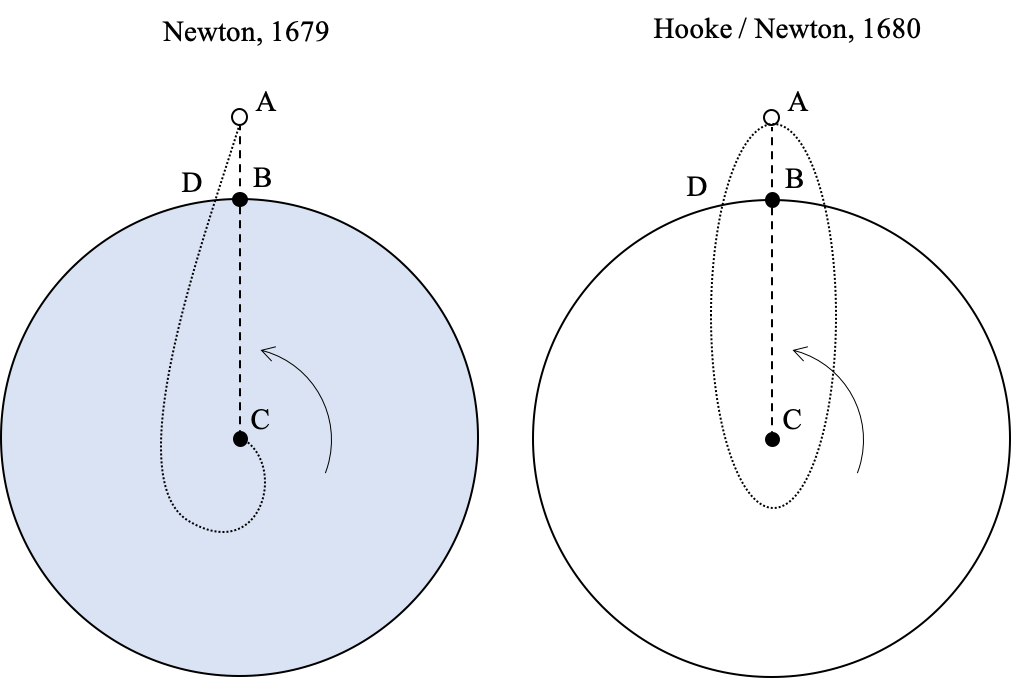
\includegraphics[width=0.8\textwidth]{./figures/horizontal_hooke_newton.png}
\caption{Izquierda: ilustración de Newton adaptada de la correspondencia
con Hooke en 1679 y en la que explicaba la trayectoria que seguiría una
partícula soltada desde el reposo en un punto A a una cierta altura
sobre una Tierra que rota. Para esta trayectoria Newton asumía que la
fuerza de gravedad era proporcional a la distancia al centro (que es lo
que pasaría dentro de la Tierra sólida.) Derecha: trayectoría elíptica
que seguiría la partícula si toda la masa de la Tierra estuviera
concentrada en el punto C y la fuerza variara con el inverso del
cuadrado de la distancia. Esta trayectoria fue sugerida por Robert Hooke
e inspiro a Newton a demostrar la primera ley de Kepler usando su teoría
de la gravedad.\label{fig:hooke_newton}}
\end{figure}

\begin{figure}[t!]
\centering
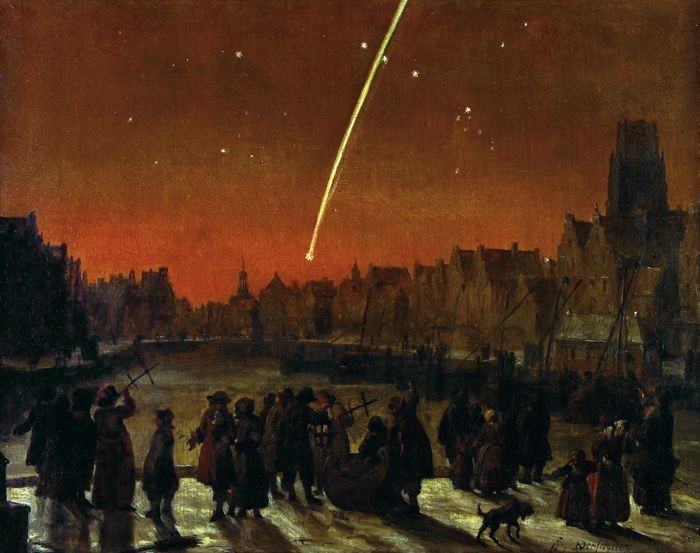
\includegraphics[width=0.8\textwidth]{./figures/square_cometa_1680.png}
\caption{Pintura del holandés Lieve Verschuier que muestra la apariencia
del gran cometa de 1680, llamado también el cometa de Newton. Crédito:
Museo de Rotterdam.\label{fig:cometa_1680}}
\end{figure}



\hypertarget{orbita_espacio}{%
\section{La órbita en el espacio}\label{orbita_espacio}}

En las secciones precedentes encontramos, usando las constantes de
movimiento del problema relativo de dos cuerpos, la ecuación de la curva
que describe el vector relativo (Ec. \ref{eq:doscuerpos_trayectoria}) y
de allí las ecuaciones de las trayectorias descritas por los cuerpos
individuales (Ecs. \ref{eq:doscuerpos_trayectoria_m1} y
\ref{eq:doscuerpos_trayectoria_m2}).

Estos resultados implican que una vez se específica un único parámetro
\(f\), es posible calcular la posición y velocidad relativa de los dos
cuerpos en el sistema de coordenadas natural de la cónica que describen
(origen en uno de los focos, semieje \(x+\) que coincide con el eje de
simetría y apuntando hacia el periapsis.)

En las siguientes secciones intentaremos resolver dos problemas
clásicos:

\begin{enumerate}
\def\labelenumi{\arabic{enumi}.}
\item
  \textbf{Determinación de órbita}. Si se conoce la posición y velocidad
  relativa instantanea de un sistema de dos cuerpos, referida a un
  sistema de coordenadas arbitrario, ¿cuál es son los elementos
  orbitales \((p,e,i,\Omega,\omega,f_0)\) que describen la cónica?
\item
  \textbf{Predicción del vector estado}. Una vez se conocen los
  elementos orbitales de un sistema de dos cuerpos
  \((p,e,i,\Omega,\omega,f_0)\) ¿cuál es el vector de estado del sistema
  (y de las partículas constituyentes) para cualquier valor de \(f\)?
\end{enumerate}

\hypertarget{determinacion_orbita}{%
\subsection{Determinación de la órbita}\label{determinacion_orbita}}

En la \autoref{fig:determinacion_orbita} se muestra la posición y
velocidad relativa instantánea de un sistema de dos cuerpos en un
sistema de coordenadas arbitrario \(x-y-z\). El reto consiste es
encontrar a partir únicamente de \(\vec r\) y \(\dot{\vec r}\), los
parámetros geométricos de la cónica \(p\) y \(e\), su orientación en el
espacio específicada por los ángulos \(i\), \(\Omega\) y \(\omega\),
además del valor de la anomalía \(f_0\) correspondiente a la posición
relativa del sistema.

\begin{figure}[t!]
\centering
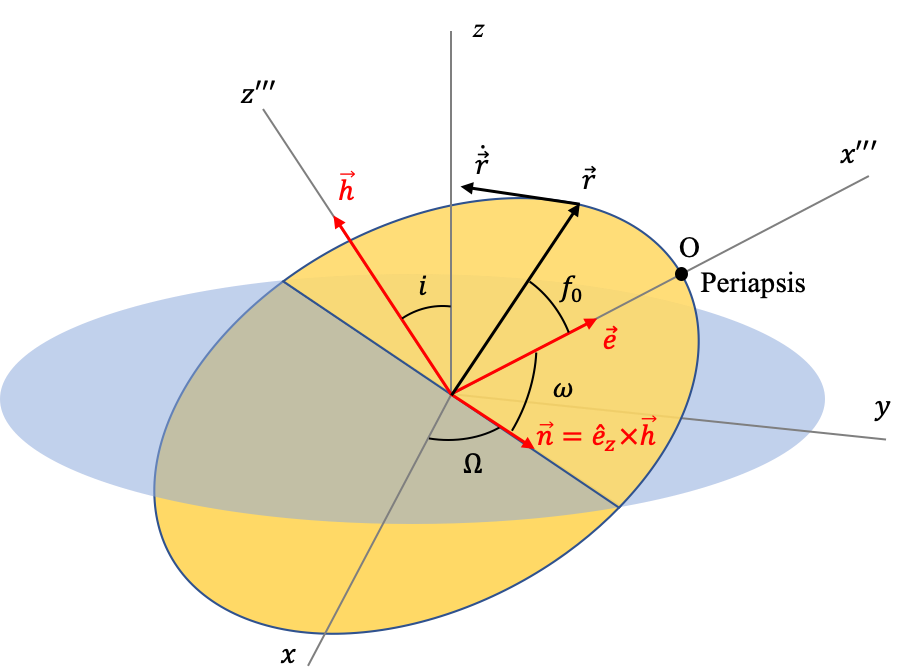
\includegraphics[width=1.0\textwidth]{./figures/square_determinacion_orbita.png}
\caption{Construcción geométrica requerida para resolver el problema de
la determinación de los elementos orbitales de la trayectoria del vector
relativo a partir del vector de estado
\(\vec X=({\vec r}\;\dot{\vec r})^\mathrm{T}\).\label{fig:determinacion_orbita}}
\end{figure}

La reconstrucción comienza por encontrar los vectores constantes:

\begin{eqnarray}
\label{eq:det_hvec}
\vec{h} & = & \vec{r}\times\dot{\vec{r}}\\
\label{eq:det_evec}
\vec{e} & = & \frac{\dot{\vec{r}} \times \vec{h}}{\mu} - \frac{\vec{r}}{r}\\
\label{eq:det_nvec}
\vec{n} & = & {\hat e}_z\times {\vec h} \\
\end{eqnarray}

De aquí se pueden obtener los parámetros de tamaño y forma de la cónica:

\begin{eqnarray}
\label{eq:det_p}
p & = & \frac{h^2}{\mu}\\
\label{eq:det_e}
e & = & |\vec{e}|
\end{eqnarray}

La orientación de la cónica puede obtenerse usando el producto escalar
entre los vectores claves:

\begin{eqnarray}
\label{eq:det_i}
\cos i & = & \frac{\vec{h}\cdot \hat{a_z}}{h} = \frac{h_z}{h} \\
\label{eq:det_W}
\cos \Omega & = & \frac{\vec{n}\cdot \hat{a_x}}{n} = \frac{n_x}{n}\\
\label{eq:det_w}
\cos \omega & = & \frac{\vec{n}\cdot \vec{e} }{ne} \\
\end{eqnarray}

Numéricamente, la función \(\theta=\cos^{-1} x\) devuelve un ángulo en
el rango \(0\leq\theta\leq\pi\). Esto es suficiente para determinar la
\emph{inclinación orbital} \(i\), pero no lo es en el caso de la
\emph{longitud del nodo ascendente} \(\Omega\) que es un ángulo en el
rango \(0\leq\Omega\leq 2\pi\), ni tampoco en el caso del
\emph{argumento del periapsis} que tiene un rango similar. En estos dos
casos podemos usar la siguientes reglas para determinar el cuadrante
correcto para los ángulos respectivos:

\begin{itemize}
\item
  \textbf{Longitud del nodo ascendente \(\Omega\)}. El criterio para
  determinar el cuadrante correcto de este elemento, parte de calcular
  la proyección del vector nodal \(\vec{n}\) sobre el eje \(y\). Si el
  signo es positivo, el valor de \(\Omega\) será el valor principal
  devuelto por \(\cos^{-1}\):

  \[
  \Omega_p\equiv\cos^{-1}\left(\frac{n_x}{n}\right)
  \]

  En caso contrario, usaremos el ángulo complementario a \(2\pi\). En
  síntesis:

  \begin{equation}
  \label{eq:W_cuadrante}
  \Omega =
  \left\{
  \begin{array}{ll}
  \Omega_p & \mathrm{Si}\;n_y \geq 0\\
  2\pi-\Omega_p & \mathrm{Si}\;n_y < 0\\
  \end{array}
  \right.
  \end{equation}
\end{itemize}

\begin{itemize}
\item
  \textbf{Argumento del periapsis \(\omega\)}. En este caso el valor
  principal del elemento es:

  \[
  \omega_p\equiv\cos^{-1}\left(\frac{\vec{n}\cdot\vec{e}}{en}\right)
  \]

  para determinar el cuadrante correcto, proyectamos el vector de
  excentricidad sobre el eje \(z\). Con esto \(\omega\) queda:

  \begin{equation}
  \label{eq:w_cuadrante}
  \omega =
  \left\{
  \begin{array}{ll}
  \omega_p & \mathrm{Si}\;e_z \geq 0\\
  2\pi-\omega_p & \mathrm{Si}\;e_z < 0\\
  \end{array}
  \right.
  \end{equation}
\end{itemize}

Finalmente la anomalía verdadera instantánea se puede determinar de la
proyección del vector posición sobre el vector excentricidad:

\begin{equation}
\label{eq:det_f}
f_p \equiv \cos^{-1}\left(\frac{\vec{e}\cdot \vec{r}}{er}\right)
\end{equation}

El cuadrante del ángulo en este caso se encuentra determinando si el
vector relativo se aleja (\(0<f<\pi\)) o se acerca al periapsis
(\(\pi<f<2\pi\)). Esta condición puede evaluarse si se calcula la
proyección del vector velocidad sobre el vector posición:

\[
v_r = \frac{\vec{r}\cdot \vec{v}}{r}
\]

Finalmente, el valor \(f\) en el cuadrante correcto:

\begin{equation}
\label{eq:f_cuadrante}
f =
\left\{
\begin{array}{ll}
f_p & \mathrm{Si}\;v_r \geq 0\\
2\pi-f_p & \mathrm{Si}\;v_r < 0\\
\end{array}
\right.
\end{equation}

\hypertarget{prediccion_estado}{%
\subsection{Predicción del vector de estado}\label{prediccion_estado}}

Una vez hemos calculado los elementos orbitales
\((p,e,i,\Omega,\omega,f_0)\) a partir de una posición específica o nos
son provistos para una trayectoria particular, el siguiente problema
consiste en determinar la posición y velocidad relativa (vecto de
estado) del sistema para un valor cualquiera de la anomalía verdadera
\(f\).

En la \autoref{elementos_orbitales} habíamos visto cómo calcular las
coordenadas de la partícula a partir de los elementos orbitales, para
una anomalía verdadera \(f\) (Ecs. \ref{eq:elementos_estado_f}):

\[
\begin{array}{rcl}
x & = & r[\cos \Omega \cos(\omega+f) - \cos i \sin \Omega \sin(\omega+f)]\\
y & = & r[\sin \Omega \cos(\omega+f) + \cos i \cos \Omega \sin(\omega+f)]\\
z & = & r \sin i \sin(\omega+f)\\ 
\end{array}
\] donde \(r=p/(1+e\cos f)\)

Las componentes cartesianas de la velocidad en el espacio se pueden
obtener partiendo de sus componentes en el sistema de coordenadas
natural de la cónica (Ecs. \ref{eq:v_hodografo}):

\begin{eqnarray}
\nonumber
\dot x''' & = & -\frac{\mu}{h} \sin f\\
\nonumber
\dot y''' & = & \frac{\mu}{h} (e+\cos f)\\
\nonumber
\dot z''' & = & 0
\end{eqnarray} que pueden, usando las expresiones explícitas para la
rotación en tres dimensiones dadas por las Ecs.
(\ref{eq:rotacion3d_natural_M}) y
(\ref{eq:matrizM_explicita_transpuesta}), rotarse al sistema del
observador:

\begin{eqnarray}
\label{eq:elementos_dotx}
\dot x = &   & \frac{\mu}{h}[-\cos \Omega \sin(\omega+f) - \cos i \sin \Omega \cos(\omega+f)]\\
\nonumber
         & - & \frac{\mu e}{h}(\cos \Omega \sin\omega + \cos\omega\cos i\sin\Omega)\\
\label{eq:elementos_doty}    
\dot y = &   & \frac{\mu}{h}[-\sin \Omega \sin(\omega+f) + \cos i \cos \Omega \cos(\omega+f)]\\
\nonumber
         & + & \frac{\mu e}{h}(-\sin \Omega \sin\omega + \cos\omega\cos i\cos\Omega)\\
\label{eq:elementos_dotz}
\dot z = &   & \frac{\mu}{h}[\sin i\cos(\omega+f) + e\cos \omega\sin i]\\ 
\end{eqnarray}

\hypertarget{orbita_osculatriz}{%
\subsection{La órbita osculatriz}\label{orbita_osculatriz}}

La existencia de una \emph{función} que asigna a cada vector de estado
\(\vec x:(x,y,z,v_x,v_y,v_z)\) un conjunto de elementos orbitales
\(p(\vec x)\), \(e(\vec x)\), \(i(\vec x)\), \(\Omega(\vec x)\),
\(\omega(\vec x)\), \(f(\vec x)\) y viceversa (Ecs.
\ref{eq:det_p}-\ref{eq:elementos_dotz}) es una interesante propiedad que
conduce a una importante definición en mecánica celeste.

\begin{figure}[t!]
\centering
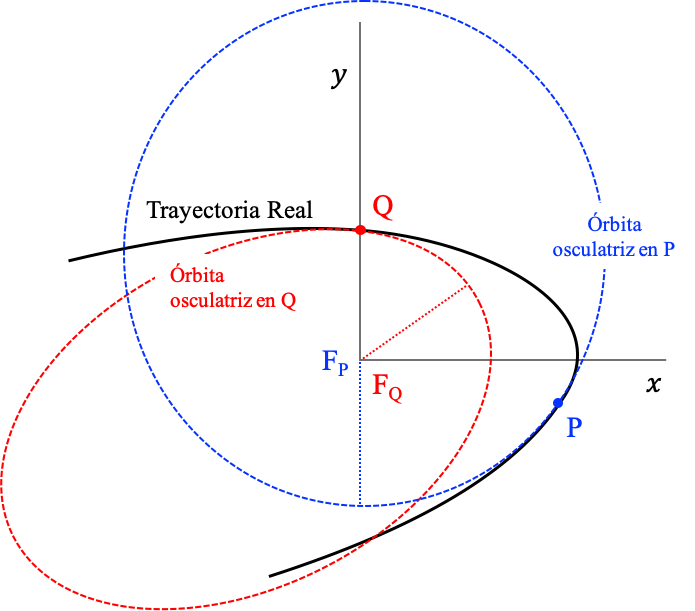
\includegraphics[width=0.5\textwidth]{./figures/square_osculatriz.png}
\caption{Ilutración del concepto de órbita osculatriz. La trayectoria
del cuerpo (curva continua) no es una cónica. Sin embargo por cada punto
de la curva (p.e. los puntos P y Q) podemos encontrar una cónica que sea
tangente a la curva (curvas rayadas) y que tenga como foco (\(F_P\) o
\(F_Q\)) el origen de coordenadas.\label{fig:osculatriz}}
\end{figure}

Independientemente de cuál es la trayectoria que siga una partícula en
el espacio, sea esta una cónica o no, siempre es posible encontrar para
cada punto de la trayectoria, una curva cónica con elementos
\(p(\vec x)\), \(e(\vec x)\), \(i(\vec x)\), \(\Omega(\vec x)\),
\(\omega(\vec x)\), \(f(\vec x)\) que tiene como foco el origen de
coordenadas y es tangente a la trayectoria de la partícula (ver
\autoref{fig:osculatriz}.) Por su naturaleza ``rasante'', llamamos a
esta cónica la \textbf{órbita osculatriz} o \textbf{cónica osculatriz}
(la palabra osculatriz viene del latin \emph{osculo} que significa
``beso''.)

Naturalmente, en el problema relativo de los dos cuerpos, la cónica
osculatriz asociada a cada punto de la trayectoria descrita por el
vector relativo será siempre la misma. En otros términos, podemos decir
que los elementos orbitales \(p(\vec x)\), \(e(\vec x)\), \(i(\vec x)\),
\(\Omega(\vec x)\), \(\omega(\vec x)\), \(f(\vec x)\) son en sí mismos
constantes de movimiento en el problema de los dos cuerpos (un
interesante resultado sobre el que volveremos en el
\autoref{formalismo_hamilton_jacobi}).

En situaciones más generales (como veremos en la
\autoref{doscuerpos_aproximacion_jerarquicos}), los elementos de la
órbita osculatriz cambian punto a punto y el estudio de su
\emph{dinámica} (conocido en mecánica celeste como \emph{teoría de
perturbaciones}) se vuelve en sí mismo muy interesante. Si bien la
teoría de perturbaciones está más allá del objetivo de este libro (es de
esos temas desarrollados en detalle en la mayoría de los textos
avanzados de mecánica celeste), por su importancia abordaremos algunos
de sus rudimentos más adelante en este capítulo.

\hypertarget{ejemplo_numerico_orbita_espacio}{%
\subsection{Un ejemplo numérico}\label{ejemplo_numerico_orbita_espacio}}

Para poner en práctica lo visto en esta sección partamos de un sistema
de dos cuerpos con condiciones iniciales arbitrarias:

    \begin{code}{}{}\begin{Verbatim}[fontsize=\small,commandchars=\\\{\}]
\PY{k+kn}{from} \PY{n+nn}{numpy} \PY{k}{import} \PY{n}{array}
\PY{n}{sistema}\PY{o}{=}\PY{p}{[}
    \PY{n+nb}{dict}\PY{p}{(}\PY{n}{m}\PY{o}{=}\PY{l+m+mf}{1.0}\PY{p}{,}
         \PY{n}{r}\PY{o}{=}\PY{n}{array}\PY{p}{(}\PY{p}{[}\PY{l+m+mf}{0.0}\PY{p}{,}\PY{l+m+mf}{0.0}\PY{p}{,}\PY{o}{+}\PY{l+m+mf}{0.3}\PY{p}{]}\PY{p}{)}\PY{p}{,}
         \PY{n}{v}\PY{o}{=}\PY{n}{array}\PY{p}{(}\PY{p}{[}\PY{o}{+}\PY{l+m+mf}{1.0}\PY{p}{,}\PY{l+m+mf}{0.0}\PY{p}{,}\PY{l+m+mf}{0.5}\PY{p}{]}\PY{p}{)}\PY{p}{)}\PY{p}{,}
    \PY{n+nb}{dict}\PY{p}{(}\PY{n}{m}\PY{o}{=}\PY{l+m+mf}{0.5}\PY{p}{,}
         \PY{n}{r}\PY{o}{=}\PY{n}{array}\PY{p}{(}\PY{p}{[}\PY{o}{+}\PY{l+m+mf}{1.0}\PY{p}{,}\PY{l+m+mf}{0.0}\PY{p}{,}\PY{l+m+mf}{0.0}\PY{p}{]}\PY{p}{)}\PY{p}{,}
         \PY{n}{v}\PY{o}{=}\PY{n}{array}\PY{p}{(}\PY{p}{[}\PY{l+m+mf}{0.0}\PY{p}{,}\PY{o}{+}\PY{l+m+mf}{1.0}\PY{p}{,}\PY{l+m+mf}{0.0}\PY{p}{]}\PY{p}{)}\PY{p}{)}\PY{p}{,}
\PY{p}{]}
\end{Verbatim}

%%

\end{code}

A partir de estas condiciones iniciales, podemos calcular los parámetros
iniciales del sistema relativo:

    \begin{code}{}{}\begin{Verbatim}[fontsize=\small,commandchars=\\\{\}]
\PY{k+kn}{from} \PY{n+nn}{numpy}\PY{n+nn}{.}\PY{n+nn}{linalg} \PY{k}{import} \PY{n}{norm}
\PY{n}{mu}\PY{o}{=}\PY{n}{sistema}\PY{p}{[}\PY{l+m+mi}{0}\PY{p}{]}\PY{p}{[}\PY{l+s+s2}{\PYZdq{}}\PY{l+s+s2}{m}\PY{l+s+s2}{\PYZdq{}}\PY{p}{]}\PY{o}{+}\PY{n}{sistema}\PY{p}{[}\PY{l+m+mi}{1}\PY{p}{]}\PY{p}{[}\PY{l+s+s2}{\PYZdq{}}\PY{l+s+s2}{m}\PY{l+s+s2}{\PYZdq{}}\PY{p}{]}
\PY{n}{rvec}\PY{o}{=}\PY{n}{sistema}\PY{p}{[}\PY{l+m+mi}{0}\PY{p}{]}\PY{p}{[}\PY{l+s+s2}{\PYZdq{}}\PY{l+s+s2}{r}\PY{l+s+s2}{\PYZdq{}}\PY{p}{]}\PY{o}{\PYZhy{}}\PY{n}{sistema}\PY{p}{[}\PY{l+m+mi}{1}\PY{p}{]}\PY{p}{[}\PY{l+s+s2}{\PYZdq{}}\PY{l+s+s2}{r}\PY{l+s+s2}{\PYZdq{}}\PY{p}{]}
\PY{n}{r}\PY{o}{=}\PY{n}{norm}\PY{p}{(}\PY{n}{rvec}\PY{p}{)}
\PY{n}{vvec}\PY{o}{=}\PY{n}{sistema}\PY{p}{[}\PY{l+m+mi}{0}\PY{p}{]}\PY{p}{[}\PY{l+s+s2}{\PYZdq{}}\PY{l+s+s2}{v}\PY{l+s+s2}{\PYZdq{}}\PY{p}{]}\PY{o}{\PYZhy{}}\PY{n}{sistema}\PY{p}{[}\PY{l+m+mi}{1}\PY{p}{]}\PY{p}{[}\PY{l+s+s2}{\PYZdq{}}\PY{l+s+s2}{v}\PY{l+s+s2}{\PYZdq{}}\PY{p}{]}
\PY{n}{v}\PY{o}{=}\PY{n}{norm}\PY{p}{(}\PY{n}{vvec}\PY{p}{)}
\end{Verbatim}

%%

\end{code}
\vspace{-1em}

%%hidecode


    \begin{Verbatim}[fontsize=\small,commandchars=\\\{\}]
mu = 1.5
r\_vec = [-1.   0.   0.3]
r = 1.044030650891055
v\_vec = [ 1.  -1.   0.5]
v = 1.5
\end{Verbatim}

A partir de los vectores posición y velocidad podemos obtener los
vectores clave (Ecs. \ref{eq:det_h}-\ref{eq:det_n}):

    \begin{code}{}{}\begin{Verbatim}[fontsize=\small,commandchars=\\\{\}]
\PY{k+kn}{from} \PY{n+nn}{numpy} \PY{k}{import} \PY{n}{cross}
\PY{k+kn}{from} \PY{n+nn}{numpy}\PY{n+nn}{.}\PY{n+nn}{linalg} \PY{k}{import} \PY{n}{norm}

\PY{c+c1}{\PYZsh{}Momento angular relativo específico}
\PY{n}{hvec}\PY{o}{=}\PY{n}{cross}\PY{p}{(}\PY{n}{rvec}\PY{p}{,}\PY{n}{vvec}\PY{p}{)}
\PY{n}{h}\PY{o}{=}\PY{n}{norm}\PY{p}{(}\PY{n}{hvec}\PY{p}{)}
\PY{c+c1}{\PYZsh{}Vector excentricidad}
\PY{n}{evec}\PY{o}{=}\PY{n}{cross}\PY{p}{(}\PY{n}{vvec}\PY{p}{,}\PY{n}{hvec}\PY{p}{)}\PY{o}{/}\PY{n}{mu}\PY{o}{\PYZhy{}}\PY{n}{rvec}\PY{o}{/}\PY{n}{r}
\PY{n}{e}\PY{o}{=}\PY{n}{norm}\PY{p}{(}\PY{n}{evec}\PY{p}{)}
\PY{c+c1}{\PYZsh{}Vector nodo ascendente}
\PY{n}{nvec}\PY{o}{=}\PY{n}{cross}\PY{p}{(}\PY{p}{[}\PY{l+m+mi}{0}\PY{p}{,}\PY{l+m+mi}{0}\PY{p}{,}\PY{l+m+mi}{1}\PY{p}{]}\PY{p}{,}\PY{n}{hvec}\PY{p}{)}
\PY{n}{n}\PY{o}{=}\PY{n}{norm}\PY{p}{(}\PY{n}{nvec}\PY{p}{)}
\end{Verbatim}

%%

\end{code}
\vspace{-1em}

%%hidecode


    \begin{Verbatim}[fontsize=\small,commandchars=\\\{\}]
hvec = [0.3 0.8 1. ]
h = 1.3152946437965904
evec = [ 0.02449295 -0.56666667  0.44598545]
e = 0.7215358864417007
nvec = [-0.8  0.3  0. ]
n = 0.8544003745317532
\end{Verbatim}

Los parámetros de tamaño y forma se obtienen usando:

    \begin{code}{}{}\begin{Verbatim}[fontsize=\small,commandchars=\\\{\}]
\PY{c+c1}{\PYZsh{}Semilatus rectum}
\PY{n}{p}\PY{o}{=}\PY{n}{h}\PY{o}{*}\PY{o}{*}\PY{l+m+mi}{2}\PY{o}{/}\PY{n}{mu}
\PY{c+c1}{\PYZsh{}Semieje mayor}
\PY{n}{a}\PY{o}{=}\PY{n}{p}\PY{o}{/}\PY{p}{(}\PY{l+m+mi}{1}\PY{o}{\PYZhy{}}\PY{n}{e}\PY{o}{*}\PY{o}{*}\PY{l+m+mi}{2}\PY{p}{)}
\PY{c+c1}{\PYZsh{}Velocidad angular promedio}
\PY{k+kn}{from} \PY{n+nn}{numpy} \PY{k}{import} \PY{n}{sqrt}
\PY{n}{nmed}\PY{o}{=}\PY{n}{sqrt}\PY{p}{(}\PY{n}{mu}\PY{o}{/}\PY{n+nb}{abs}\PY{p}{(}\PY{n}{a}\PY{p}{)}\PY{o}{*}\PY{o}{*}\PY{l+m+mi}{3}\PY{p}{)}
\end{Verbatim}

%%

\end{code}
\vspace{-1em}

%%hidecode


    \begin{Verbatim}[fontsize=\small,commandchars=\\\{\}]
p = 1.153333333333333 u.c.
a = 2.405855445416549 u.c.
nmed = 0.3282020847560834 u.c.
\end{Verbatim}

La orientación de la órbita se obtiene usando las Ecs.
(\ref{eq:det_W})-(\ref{eq:det_f}):

    \begin{code}{}{}\begin{Verbatim}[fontsize=\small,commandchars=\\\{\}]
\PY{k+kn}{from} \PY{n+nn}{numpy} \PY{k}{import} \PY{n}{dot}\PY{p}{,}\PY{n}{arccos}\PY{p}{,}\PY{n}{pi}
\PY{n}{i}\PY{o}{=}\PY{n}{arccos}\PY{p}{(}\PY{n}{hvec}\PY{p}{[}\PY{l+m+mi}{2}\PY{p}{]}\PY{o}{/}\PY{n}{h}\PY{p}{)}

\PY{n}{Wp}\PY{o}{=}\PY{n}{arccos}\PY{p}{(}\PY{n}{nvec}\PY{p}{[}\PY{l+m+mi}{0}\PY{p}{]}\PY{o}{/}\PY{n}{n}\PY{p}{)}
\PY{n}{W}\PY{o}{=}\PY{n}{Wp} \PY{k}{if} \PY{n}{nvec}\PY{p}{[}\PY{l+m+mi}{1}\PY{p}{]}\PY{o}{\PYZgt{}}\PY{l+m+mi}{0} \PY{k}{else} \PY{l+m+mi}{2}\PY{o}{*}\PY{n}{pi}\PY{o}{\PYZhy{}}\PY{n}{Wp}

\PY{n}{wp}\PY{o}{=}\PY{n}{arccos}\PY{p}{(}\PY{n}{dot}\PY{p}{(}\PY{n}{nvec}\PY{p}{,}\PY{n}{evec}\PY{p}{)}\PY{o}{/}\PY{p}{(}\PY{n}{e}\PY{o}{*}\PY{n}{n}\PY{p}{)}\PY{p}{)}
\PY{n}{w}\PY{o}{=}\PY{n}{wp} \PY{k}{if} \PY{n}{evec}\PY{p}{[}\PY{l+m+mi}{2}\PY{p}{]}\PY{o}{\PYZgt{}}\PY{l+m+mi}{0} \PY{k}{else} \PY{l+m+mi}{2}\PY{o}{*}\PY{n}{pi}\PY{o}{\PYZhy{}}\PY{n}{wp}

\PY{n}{fp}\PY{o}{=}\PY{n}{arccos}\PY{p}{(}\PY{n}{dot}\PY{p}{(}\PY{n}{rvec}\PY{p}{,}\PY{n}{evec}\PY{p}{)}\PY{o}{/}\PY{p}{(}\PY{n}{r}\PY{o}{*}\PY{n}{e}\PY{p}{)}\PY{p}{)}
\PY{n}{f0}\PY{o}{=}\PY{n}{fp} \PY{k}{if} \PY{n}{dot}\PY{p}{(}\PY{n}{rvec}\PY{p}{,}\PY{n}{vvec}\PY{p}{)}\PY{o}{\PYZgt{}}\PY{l+m+mi}{0} \PY{k}{else} \PY{l+m+mi}{2}\PY{o}{*}\PY{n}{pi}\PY{o}{\PYZhy{}}\PY{n}{fp}
\end{Verbatim}

%%

\end{code}
\vspace{-1em}

%%hidecode


    \begin{Verbatim}[fontsize=\small,commandchars=\\\{\}]
i = 40.510589437332754 grados
W = 159.44395478041653 grados
w = 107.91123121198778 grados
f\_0 = 278.34291953929824 grados
\end{Verbatim}

Hemos sintetizado este mismo procedimiento como la rutina
\texttt{estado\_a\_elementos} cuyo algoritmo se presenta en el
{[}Apéndice \emph{Algoritmos y rutinas útiles}{]}.

Con este resultado podemos ahora determinar el vector posición y
velocidad en un valor arbitario de la anomalía verdadera:

    \begin{code}{}{}\begin{Verbatim}[fontsize=\small,commandchars=\\\{\}]
\PY{c+c1}{\PYZsh{}Anomalía verdadera}
\PY{n}{f}\PY{o}{=}\PY{n}{pi}\PY{o}{/}\PY{l+m+mi}{2}

\PY{c+c1}{\PYZsh{}Distancia al punto}
\PY{k+kn}{from} \PY{n+nn}{numpy} \PY{k}{import} \PY{n}{cos}
\PY{n}{r}\PY{o}{=}\PY{n}{p}\PY{o}{/}\PY{p}{(}\PY{l+m+mi}{1}\PY{o}{+}\PY{n}{e}\PY{o}{*}\PY{n}{cos}\PY{p}{(}\PY{n}{f}\PY{p}{)}\PY{p}{)}
\end{Verbatim}

%%

\end{code}

Las coordenadas del punto son:

    \begin{code}{}{}\begin{Verbatim}[fontsize=\small,commandchars=\\\{\}]
\PY{k+kn}{from} \PY{n+nn}{numpy} \PY{k}{import} \PY{n}{cos}\PY{p}{,}\PY{n}{sin}
\PY{n}{x}\PY{o}{=}\PY{n}{r}\PY{o}{*}\PY{p}{(}\PY{n}{cos}\PY{p}{(}\PY{n}{W}\PY{p}{)}\PY{o}{*}\PY{n}{cos}\PY{p}{(}\PY{n}{w}\PY{o}{+}\PY{n}{f}\PY{p}{)}\PY{o}{\PYZhy{}}\PY{n}{cos}\PY{p}{(}\PY{n}{i}\PY{p}{)}\PY{o}{*}\PY{n}{sin}\PY{p}{(}\PY{n}{W}\PY{p}{)}\PY{o}{*}\PY{n}{sin}\PY{p}{(}\PY{n}{w}\PY{o}{+}\PY{n}{f}\PY{p}{)}\PY{p}{)}
\PY{n}{y}\PY{o}{=}\PY{n}{r}\PY{o}{*}\PY{p}{(}\PY{n}{sin}\PY{p}{(}\PY{n}{W}\PY{p}{)}\PY{o}{*}\PY{n}{cos}\PY{p}{(}\PY{n}{w}\PY{o}{+}\PY{n}{f}\PY{p}{)}\PY{o}{+}\PY{n}{cos}\PY{p}{(}\PY{n}{i}\PY{p}{)}\PY{o}{*}\PY{n}{cos}\PY{p}{(}\PY{n}{W}\PY{p}{)}\PY{o}{*}\PY{n}{sin}\PY{p}{(}\PY{n}{w}\PY{o}{+}\PY{n}{f}\PY{p}{)}\PY{p}{)}
\PY{n}{z}\PY{o}{=}\PY{n}{r}\PY{o}{*}\PY{n}{sin}\PY{p}{(}\PY{n}{i}\PY{p}{)}\PY{o}{*}\PY{n}{sin}\PY{p}{(}\PY{n}{w}\PY{o}{+}\PY{n}{f}\PY{p}{)}

\PY{k+kn}{from} \PY{n+nn}{numpy} \PY{k}{import} \PY{n}{array}
\PY{n}{r\PYZus{}nuevo}\PY{o}{=}\PY{n}{array}\PY{p}{(}\PY{p}{[}\PY{n}{x}\PY{p}{,}\PY{n}{y}\PY{p}{,}\PY{n}{z}\PY{p}{]}\PY{p}{)}
\end{Verbatim}

%%

\end{code}

Y la velocidad:

    \begin{code}{}{}\begin{Verbatim}[fontsize=\small,commandchars=\\\{\}]
\PY{c+c1}{\PYZsh{}Parametro mu/h}
\PY{n}{muh}\PY{o}{=}\PY{n}{mu}\PY{o}{/}\PY{n}{h}

\PY{n}{vx}\PY{o}{=}\PY{n}{muh}\PY{o}{*}\PY{p}{(}\PY{o}{\PYZhy{}}\PY{n}{cos}\PY{p}{(}\PY{n}{W}\PY{p}{)}\PY{o}{*}\PY{n}{sin}\PY{p}{(}\PY{n}{w}\PY{o}{+}\PY{n}{f}\PY{p}{)}\PY{o}{\PYZhy{}}\PY{n}{cos}\PY{p}{(}\PY{n}{i}\PY{p}{)}\PY{o}{*}\PY{n}{sin}\PY{p}{(}\PY{n}{W}\PY{p}{)}\PY{o}{*}\PY{n}{cos}\PY{p}{(}\PY{n}{w}\PY{o}{+}\PY{n}{f}\PY{p}{)}\PY{p}{)}\PYZbs{}
   \PY{o}{\PYZhy{}}\PY{n}{muh}\PY{o}{*}\PY{n}{e}\PY{o}{*}\PY{p}{(}\PY{n}{cos}\PY{p}{(}\PY{n}{W}\PY{p}{)}\PY{o}{*}\PY{n}{sin}\PY{p}{(}\PY{n}{w}\PY{p}{)}\PY{o}{+}\PY{n}{cos}\PY{p}{(}\PY{n}{w}\PY{p}{)}\PY{o}{*}\PY{n}{cos}\PY{p}{(}\PY{n}{i}\PY{p}{)}\PY{o}{*}\PY{n}{sin}\PY{p}{(}\PY{n}{W}\PY{p}{)}\PY{p}{)}
\PY{n}{vy}\PY{o}{=}\PY{n}{muh}\PY{o}{*}\PY{p}{(}\PY{o}{\PYZhy{}}\PY{n}{sin}\PY{p}{(}\PY{n}{W}\PY{p}{)}\PY{o}{*}\PY{n}{sin}\PY{p}{(}\PY{n}{w}\PY{o}{+}\PY{n}{f}\PY{p}{)}\PY{o}{+}\PY{n}{cos}\PY{p}{(}\PY{n}{i}\PY{p}{)}\PY{o}{*}\PY{n}{cos}\PY{p}{(}\PY{n}{W}\PY{p}{)}\PY{o}{*}\PY{n}{cos}\PY{p}{(}\PY{n}{w}\PY{o}{+}\PY{n}{f}\PY{p}{)}\PY{p}{)}\PYZbs{}
   \PY{o}{+}\PY{n}{muh}\PY{o}{*}\PY{n}{e}\PY{o}{*}\PY{p}{(}\PY{o}{\PYZhy{}}\PY{n}{sin}\PY{p}{(}\PY{n}{W}\PY{p}{)}\PY{o}{*}\PY{n}{sin}\PY{p}{(}\PY{n}{w}\PY{p}{)}\PY{o}{+}\PY{n}{cos}\PY{p}{(}\PY{n}{w}\PY{p}{)}\PY{o}{*}\PY{n}{cos}\PY{p}{(}\PY{n}{i}\PY{p}{)}\PY{o}{*}\PY{n}{cos}\PY{p}{(}\PY{n}{W}\PY{p}{)}\PY{p}{)}
\PY{n}{vz}\PY{o}{=}\PY{n}{muh}\PY{o}{*}\PY{p}{(}\PY{n}{sin}\PY{p}{(}\PY{n}{i}\PY{p}{)}\PY{o}{*}\PY{n}{cos}\PY{p}{(}\PY{n}{w}\PY{o}{+}\PY{n}{f}\PY{p}{)}\PY{o}{+}\PY{n}{e}\PY{o}{*}\PY{n}{cos}\PY{p}{(}\PY{n}{w}\PY{p}{)}\PY{o}{*}\PY{n}{sin}\PY{p}{(}\PY{n}{i}\PY{p}{)}\PY{p}{)}

\PY{k+kn}{from} \PY{n+nn}{numpy} \PY{k}{import} \PY{n}{array}
\PY{n}{v\PYZus{}nuevo}\PY{o}{=}\PY{n}{array}\PY{p}{(}\PY{p}{[}\PY{n}{vx}\PY{p}{,}\PY{n}{vy}\PY{p}{,}\PY{n}{vz}\PY{p}{]}\PY{p}{)}
\end{Verbatim}

%%

\end{code}

Una posible comprobación de que nuestra predicción es la correcta
(aunque es una condición necesaria y no suficiente de su validez), es
verificar si el momento angular específico relativo con el vector de
estado sigue siendo el mismo:

    \begin{code}{}{}\begin{Verbatim}[fontsize=\small,commandchars=\\\{\}]
\PY{k+kn}{from} \PY{n+nn}{numpy} \PY{k}{import} \PY{n}{cross}
\PY{n}{hvec\PYZus{}nuevo}\PY{o}{=}\PY{n}{cross}\PY{p}{(}\PY{n}{r\PYZus{}nuevo}\PY{p}{,}\PY{n}{v\PYZus{}nuevo}\PY{p}{)}
\end{Verbatim}

%%

\end{code}
\vspace{-1em}

%%hidecode


    \begin{Verbatim}[fontsize=\small,commandchars=\\\{\}]
Inicial, hvec = [0.3 0.8 1. ]
Nueva posición, hvec = [0.3 0.8 1. ]
\end{Verbatim}

Y vemos que coinciden.

Una prueba aún más estricta para nuestra teoría sería la de comparar la
órbita predicha con una integración numérica de las ecuaciones de
movimiento. Para ello nos valdremos de la rutina
\texttt{ncuerpos\_solucion} definida en el Alg.
(\ref{code:ncuerpos_solucion}):

    \begin{code}{}{}\begin{Verbatim}[fontsize=\small,commandchars=\\\{\}]
\PY{c+c1}{\PYZsh{}Tiempo característico de la cónica}
\PY{c+c1}{\PYZsh{}Si la cónica es una elipse este es el período}
\PY{k+kn}{from} \PY{n+nn}{numpy} \PY{k}{import} \PY{n}{pi}
\PY{n}{T}\PY{o}{=}\PY{l+m+mi}{2}\PY{o}{*}\PY{n}{pi}\PY{o}{/}\PY{n}{nmed}

\PY{c+c1}{\PYZsh{}Tiempos }
\PY{k+kn}{from} \PY{n+nn}{numpy} \PY{k}{import} \PY{n}{linspace}
\PY{n}{ts}\PY{o}{=}\PY{n}{linspace}\PY{p}{(}\PY{l+m+mi}{0}\PY{p}{,}\PY{n}{T}\PY{p}{,}\PY{l+m+mi}{20}\PY{p}{)}

\PY{c+c1}{\PYZsh{}Solución a las e.d.m. del sistema}
\PY{k+kn}{from} \PY{n+nn}{pymcel}\PY{n+nn}{.}\PY{n+nn}{export} \PY{k}{import} \PY{n}{ncuerpos\PYZus{}solucion}
\PY{n}{rs}\PY{p}{,}\PY{n}{vs}\PY{p}{,}\PY{n}{rps}\PY{p}{,}\PY{n}{vps}\PY{p}{,}\PY{n}{constantes}\PY{o}{=}\PY{n}{ncuerpos\PYZus{}solucion}\PY{p}{(}\PY{n}{sistema}\PY{p}{,}\PY{n}{ts}\PY{p}{)}
\end{Verbatim}

%%

\end{code}

Para comparar con la solución necesitamos calcular las posiciones y
velocidades relativas. Por relativas, no es importante si usamos el
vector de estado referido al sistema de referencia original
(\texttt{rs}, \texttt{vs}) o el referido al centro de masa
(\texttt{rps},\texttt{vps}):

    \begin{code}{}{}\begin{Verbatim}[fontsize=\small,commandchars=\\\{\}]
\PY{n}{rs\PYZus{}num}\PY{o}{=}\PY{n}{rs}\PY{p}{[}\PY{l+m+mi}{0}\PY{p}{,}\PY{p}{:}\PY{p}{,}\PY{p}{:}\PY{p}{]}\PY{o}{\PYZhy{}}\PY{n}{rs}\PY{p}{[}\PY{l+m+mi}{1}\PY{p}{,}\PY{p}{:}\PY{p}{,}\PY{p}{:}\PY{p}{]}
\PY{n}{vs\PYZus{}num}\PY{o}{=}\PY{n}{vs}\PY{p}{[}\PY{l+m+mi}{0}\PY{p}{,}\PY{p}{:}\PY{p}{,}\PY{p}{:}\PY{p}{]}\PY{o}{\PYZhy{}}\PY{n}{vs}\PY{p}{[}\PY{l+m+mi}{1}\PY{p}{,}\PY{p}{:}\PY{p}{,}\PY{p}{:}\PY{p}{]}
\end{Verbatim}

%%

\end{code}

Para visualizar la órbita predicha en tres dimensiones, usaremos la
rutina \texttt{conica\_de\_elementos}:
%%HIDE%%
    \begin{code}{Algoritmo}{code:7_Problema2Cuerpos_21}\begin{Verbatim}[fontsize=\small,commandchars=\\\{\}]
\PY{c+c1}{\PYZsh{}Visualización de la cónica }
\PY{k+kn}{from} \PY{n+nn}{numpy} \PY{k}{import} \PY{n}{pi}
\PY{k+kn}{from} \PY{n+nn}{pymcel}\PY{n+nn}{.}\PY{n+nn}{export} \PY{k}{import} \PY{n}{conica\PYZus{}de\PYZus{}elementos}
\PY{n}{fig}\PY{o}{=}\PY{n}{conica\PYZus{}de\PYZus{}elementos}\PY{p}{(}\PY{n}{p}\PY{p}{,}\PY{n}{e}\PY{p}{,}\PY{n}{i}\PY{o}{*}\PY{l+m+mi}{180}\PY{o}{/}\PY{n}{pi}\PY{p}{,}\PY{n}{W}\PY{o}{*}\PY{l+m+mi}{180}\PY{o}{/}\PY{n}{pi}\PY{p}{,}\PY{n}{w}\PY{o}{*}\PY{l+m+mi}{180}\PY{o}{/}\PY{n}{pi}\PY{p}{,}\PY{n}{figreturn}\PY{o}{=}\PY{k+kc}{True}\PY{p}{)}
\PY{n}{ax}\PY{o}{=}\PY{n}{fig}\PY{o}{.}\PY{n}{gca}\PY{p}{(}\PY{p}{)}
\PY{c+c1}{\PYZsh{}Posición y velocidad inicial}
\PY{n}{ax}\PY{o}{.}\PY{n}{quiver}\PY{p}{(}\PY{l+m+mi}{0}\PY{p}{,}\PY{l+m+mi}{0}\PY{p}{,}\PY{l+m+mi}{0}\PY{p}{,}
          \PY{n}{rvec}\PY{p}{[}\PY{l+m+mi}{0}\PY{p}{]}\PY{p}{,}\PY{n}{rvec}\PY{p}{[}\PY{l+m+mi}{1}\PY{p}{]}\PY{p}{,}\PY{n}{rvec}\PY{p}{[}\PY{l+m+mi}{2}\PY{p}{]}\PY{p}{,}
          \PY{n}{color}\PY{o}{=}\PY{l+s+s1}{\PYZsq{}}\PY{l+s+s1}{k}\PY{l+s+s1}{\PYZsq{}}\PY{p}{)}\PY{p}{;}
\PY{n}{ax}\PY{o}{.}\PY{n}{quiver}\PY{p}{(}\PY{n}{rvec}\PY{p}{[}\PY{l+m+mi}{0}\PY{p}{]}\PY{p}{,}\PY{n}{rvec}\PY{p}{[}\PY{l+m+mi}{1}\PY{p}{]}\PY{p}{,}\PY{n}{rvec}\PY{p}{[}\PY{l+m+mi}{2}\PY{p}{]}\PY{p}{,}
          \PY{n}{vvec}\PY{p}{[}\PY{l+m+mi}{0}\PY{p}{]}\PY{p}{,}\PY{n}{vvec}\PY{p}{[}\PY{l+m+mi}{1}\PY{p}{]}\PY{p}{,}\PY{n}{vvec}\PY{p}{[}\PY{l+m+mi}{2}\PY{p}{]}\PY{p}{,}
          \PY{n}{color}\PY{o}{=}\PY{l+s+s1}{\PYZsq{}}\PY{l+s+s1}{k}\PY{l+s+s1}{\PYZsq{}}\PY{p}{)}\PY{p}{;}

\PY{c+c1}{\PYZsh{}Posición y velocidad nueva}
\PY{n}{ax}\PY{o}{.}\PY{n}{quiver}\PY{p}{(}\PY{l+m+mi}{0}\PY{p}{,}\PY{l+m+mi}{0}\PY{p}{,}\PY{l+m+mi}{0}\PY{p}{,}
          \PY{n}{r\PYZus{}nuevo}\PY{p}{[}\PY{l+m+mi}{0}\PY{p}{]}\PY{p}{,}\PY{n}{r\PYZus{}nuevo}\PY{p}{[}\PY{l+m+mi}{1}\PY{p}{]}\PY{p}{,}\PY{n}{r\PYZus{}nuevo}\PY{p}{[}\PY{l+m+mi}{2}\PY{p}{]}\PY{p}{,}
          \PY{n}{color}\PY{o}{=}\PY{l+s+s1}{\PYZsq{}}\PY{l+s+s1}{b}\PY{l+s+s1}{\PYZsq{}}\PY{p}{)}\PY{p}{;}
\PY{n}{ax}\PY{o}{.}\PY{n}{quiver}\PY{p}{(}\PY{n}{r\PYZus{}nuevo}\PY{p}{[}\PY{l+m+mi}{0}\PY{p}{]}\PY{p}{,}\PY{n}{r\PYZus{}nuevo}\PY{p}{[}\PY{l+m+mi}{1}\PY{p}{]}\PY{p}{,}\PY{n}{r\PYZus{}nuevo}\PY{p}{[}\PY{l+m+mi}{2}\PY{p}{]}\PY{p}{,}
          \PY{n}{v\PYZus{}nuevo}\PY{p}{[}\PY{l+m+mi}{0}\PY{p}{]}\PY{p}{,}\PY{n}{v\PYZus{}nuevo}\PY{p}{[}\PY{l+m+mi}{1}\PY{p}{]}\PY{p}{,}\PY{n}{v\PYZus{}nuevo}\PY{p}{[}\PY{l+m+mi}{2}\PY{p}{]}\PY{p}{,}
          \PY{n}{color}\PY{o}{=}\PY{l+s+s1}{\PYZsq{}}\PY{l+s+s1}{b}\PY{l+s+s1}{\PYZsq{}}\PY{p}{)}\PY{p}{;}

\PY{c+c1}{\PYZsh{}Posiciones calculadas numéricamente}
\PY{n}{ax}\PY{o}{.}\PY{n}{plot}\PY{p}{(}\PY{n}{rs\PYZus{}num}\PY{p}{[}\PY{p}{:}\PY{p}{,}\PY{l+m+mi}{0}\PY{p}{]}\PY{p}{,}\PY{n}{rs\PYZus{}num}\PY{p}{[}\PY{p}{:}\PY{p}{,}\PY{l+m+mi}{1}\PY{p}{]}\PY{p}{,}\PY{n}{rs\PYZus{}num}\PY{p}{[}\PY{p}{:}\PY{p}{,}\PY{l+m+mi}{2}\PY{p}{]}\PY{p}{,}\PY{l+s+s1}{\PYZsq{}}\PY{l+s+s1}{rx}\PY{l+s+s1}{\PYZsq{}}\PY{p}{)}\PY{p}{;}

\PY{n}{fig}\PY{o}{.}\PY{n}{tight\PYZus{}layout}\PY{p}{(}\PY{p}{)}
\end{Verbatim}

%%

\tcblower
\footnotesize
\em ver Figura \ref{fig:code:7_Problema2Cuerpos_21}
\end{code}

    \begin{center}

\begin{figure}[ht!]
\centering
    \adjustimage{max size={0.8\linewidth}{0.8\paperheight}}{combined_files/combined_1315_0.png}
\caption{Figura correspondiente al código \ref{code:7_Problema2Cuerpos_21}.\label{fig:code:7_Problema2Cuerpos_21}}
\end{figure}

    \end{center}
%{ \hspace*{\fill} \\}
    
Este resultado nos permite comprobar plenamente los resultados teóricos
de las últimas sesiones:

\begin{itemize}
\item
  La posición y velocidad inicial coincide con uno de los puntos de la
  curva cónica.
\item
  La nueva posición y velocidad coincide también con uno de los puntos
  de la cónica.
\item
  Las posiciones relativas calculadas numéricamente coinciden
  perfectamente con los puntos sobre la cónica.
\end{itemize}



\hypertarget{doscuerpos_tiempo}{%
\section{El problema de los dos cuerpos en el
tiempo}\label{doscuerpos_tiempo}}

Como vimos en la \autoref{doscuerpos_constantes}, \textbf{ninguna}
de las constantes de movimiento identificadas en el problema relativo de
los dos cuerpos, depende explícitamente del tiempo. Esto implica que con
las cuadraturas disponibles lo único que podemos hacer es expresar la
posición y velocidad en términos de un parámetro, la anomalía verdadera
\(f\) (ver \autoref{doscuerpos_ecuacion}) sin tener todavía ninguna
clave de cómo este parámetro depende del tiempo. En esta sección nos
proponemos justamente eso, encontrar la manera de calcular la anomalía
verdadera del vector relativo (o cualquiera de las otras anomalías
definidas antes) para cualquier instante del tiempo. Llamamos a este el
\emph{problema de Kepler} y su solución no es otra cosa que el objetivo
perseguido desde el principio de este libro.

Para ello debemos primero responder a la pregunta: ¿hay alguna propiedad
geométrica en el movimiento del vector relativo sobre la cónica cuyo
valor puede predecirse exactamente en el tiempo? Examinando los teoremas
del movimiento orbital (ver \autoref{teoremas_orbital}) nos damos
cuenta que la única cantidad con esta propiedad es el área \(A\) barrida
por el radio vector (area del \emph{sector de cónica}) que, deacuerdo
con el Teo. (\ref{box:teo:areas}), cambia uniformemente con el tiempo a
razón de (Ec. \ref{eq:velocidad_areal}):

\[
\frac{\mathrm{d}A}{\mathrm{d}t}=\frac{h}{2}
\]

Si integramos esta ecuación el área del sector de cónica barrida por el
vector relativo entre el tiempo de paso por el periapsis \(t_p\) y un
tiempo arbitrario \(t\) será:

\begin{equation}
\label{eq:area_sector_tiempo}
\Delta A = \frac{h}{2}(t-t_p)
\end{equation}

Ahora bien, como vimos en la \autoref{area_conicas} el área del
sector \(\Delta A\) depende explícitamente de las anomalías (verdadera o
excéntrica), de modo la Ec. (\ref{eq:area_sector_tiempo}) combinada con
la expresión explícita de \(\Delta A\) como función de las anomalías
proveerá la respuestas final a la pregunta formulada aquí.

\hypertarget{ecuacion_halley}{%
\subsection{La ecuación de Halley}\label{ecuacion_halley}}

Aunque no es común presentarlo en este orden e históricamente el caso de
la parábola fue el último en ser planteado como se muestra aquí,
comenzaremos por resolver la pregunta de cómo calcular la anomalía
verdadera del vector relativo en el problema de los dos cuerpos que se
mueven sobre una parábola, \(e=1\) (p.e. un cometa.)

En la \autoref{area_elipse} habíamos deducido geométricamente la
relación entre el área de un sector de parábola y la anomalía verdadera
correspondiente:

\[
\Delta A_\mathrm{parabola}=\frac{1}{4}p^2\left(\tan\frac{f}{2}+\frac{1}{3}\tan^3\frac{f}{2}\right)
\]

Dado que por la Ec. (\textbackslash{}ref\{eq:area\_sector\_tiempo)
sabemos cuánto vale \(\Delta A\) en cualquier tiempo, podemos escribir
explícitamente:

\[
\frac{1}{2}h(t-t_p)=\frac{1}{4}p^2\left(\tan\frac{f}{2}+\frac{1}{3}\tan^3\frac{f}{2}\right)
\]

Si usamos \(h=\sqrt{\mu p}\) obtenemos después de algunas manipulaciones
algebraicas elementales:

\begin{equation}
\label{eq:ecuacion_barker}
6\sqrt{\frac{\mu}{p^3}}(t-t_p)=\tan^3\frac{f}{2}+3\tan\frac{f}{2}
\end{equation}

Llamaremos a esta ecuación, la \textbf{ecuación de Halley} y su solución
nos brinda finalmente la respuesta a la pregunta original.
\begin{box_history}{Un poco de historia}{}{nofloat}
\small

\textbf{¿Halley o Barker?.} Es común presentar la Ec.
(\ref{eq:ecuacion_halley}) en la forma:

\[
  2\sqrt{\frac{\mu}{p^3}}(t-t_p)=\tan\frac{f}{2}+\frac{1}{3}\tan^3\frac{f}{2}
  \]

y referirse a ella como la \textbf{Ecuación de Barker}. Así lo hacen
prácticamente la totalidad de los textos de mecánica celeste escritos en
los últimos 250 años.

Una indagación histórica más juiciosa \cite{Colwell1993Kepler} ha
revelado, sin embargo, que el primero en deducir y utilizar esta
ecuación fue Edmund Halley
(\hreffoot{https://forvo.com/search/Halley/en_uk/}{``Edmond Hali''}.)

Halley (1656-1742, ver \autoref{fig:halley}) fue un virtuoso inglés
contemporáneo de Newton, cuyos trabajos científicos abarcaron áreas tan
diversas como la astronomía (en la que hizo sus principales
contribuciones), la física, la meteorología, las matemáticas y la
geofísica. Fue Halley en 1684 quién presentó a Newton el problema que
conduciría a este a su teoría general de la gravitación: qué tipo de
trayectoria seguirá un cuerpo que se mueva bajo la influencia de una
fuerza que disminuya con el cuadrado de la distancia. Newton respondió a
este problema con la monografía ``\emph{De Motu corporum in gyrum}'',
que no es otra cosa que la ``semilla'' de la Mecánica Celeste moderna.
En 1687, Halley culminó el ``trabajo editorial'' de su vida al publicar
la primera edición de los \emph{Principia} de Newton.

En 1705, más de veinte años después de la publicación de los Principia,
Halley publicá la monografía ``Una sinopsis de la astronomía de los
cometas'' \footnote{Una copia digital del manuscrito esta disponible en
  línea en https://archive.org/details/synopsisofastron00hall/page/n4}
en la que compila información observacional relacionada con los cometas
observados en su tiempo y en siglos anteriores y de provee tablas de
posiciones pasadas y futuras de esos mismos cometas. Es en este trabajo
en el que Halley introduce por primera vez la Ec.
(\ref{eq:ecuacion_halley}), la cual utiliza para el cálculo de sus
tablas. Allí, además, Halley realizá el trascendental descubrimiento por
el que sería recordado por siempre. Según sus análisis tres cometas que
habían sido observado en 1531, 1607 y 1682 (esté último observado y
registrado por él mismo) eran en realidad uno solo. Armado con la teoría
de Newton Halley predice que el cometa se aproximaría nuevamente al Sol
y a la Tierra en el año 1758. Lamentablemente no viviría lo suficiente
para hacer realidad su predicción, que se cumplió sin falta. Hoy, el
mencionado cometa lleva su nombre, 1P/Halley o ``cometa Halley''. Sus
últimas apariciones (antes de la preparación de este libro) se
produjeron en 1910 y 1986 y las próximas serán en 2061 y 2134 (ver
\autoref{fig:Halley}.)

¿Por qué entonces la mayoría de los autores llaman a la Ec.
(\ref{eq:ecuacion_halley}), ``ecuación de Barker''?

En 1757, apenas un año antes del regreso del cometa Halley, El
meteorologo inglés Thomas Barker escribió una monografía titulada ``Un
relato sobre los descubrimientos relacionados con los cometas'' en la
que no solo realizaba predicciones precisas de la posición de los
cometas sobre órbitas parabólicas sino también aplicaba los mismos
métodos teóricos para estudiar el problema más práctico del movimiento
de proyectiles. Barker uso en su trabajo la Ec.
(\ref{eq:ecuacion_halley}) para sus predicciones y no sabemos si la
dedujo por su cuenta o la tomó del trabajo de Halley (como seguramente
debió ocurrir) sin hacer necesariamente referencia a él (una práctica
común en la época, especialmente si se trataba de resultados que no erán
muy difíciles de deducir.) En 1793, el astrónomo Henry Englefield
publico su influyente libro ``Sobre la determinación de las órbitas de
los cometas'' en el que uso, entre otros, los métodos de Barker. Para
dar crédito a su autor, fue Englefield el que llamo por primera vez a la
Ec. (\ref{eq:ecuacion_halley}) ``ecuación de Barker'' y de allí se
nutrieron los autores sucesivos.

\end{box_history}
\begin{figure}[t!]
\centering
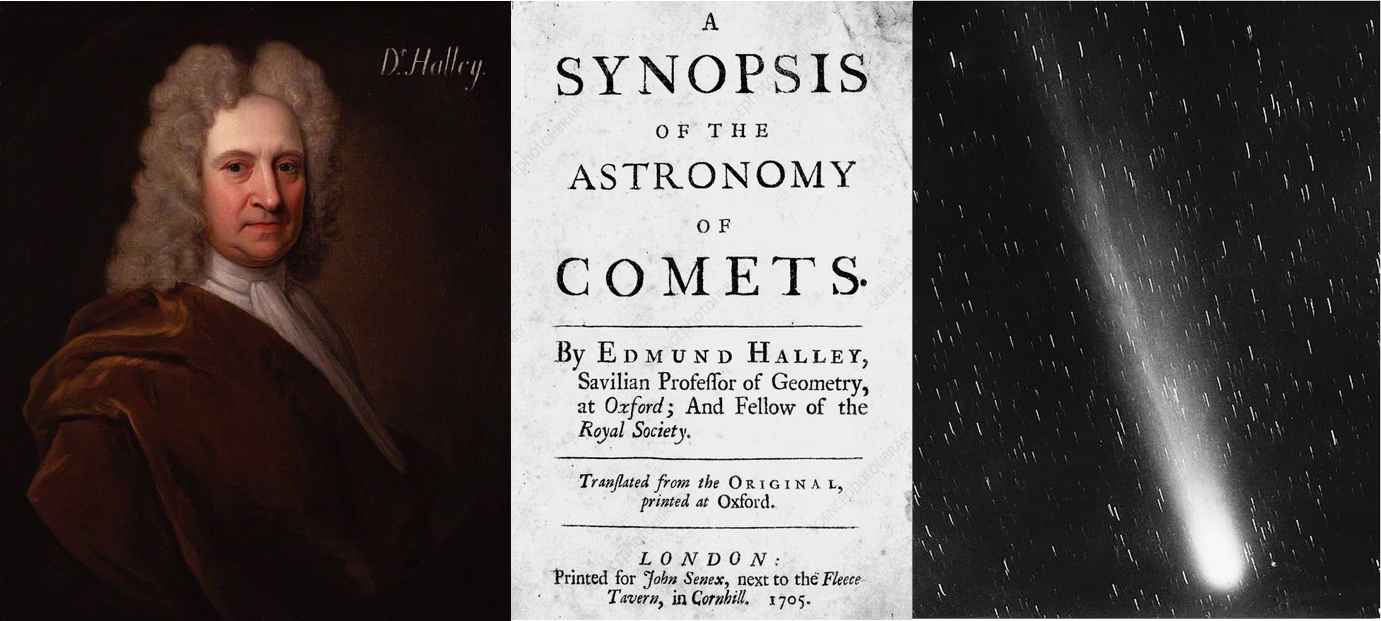
\includegraphics[width=1\textwidth]{./figures/horizontal_halley.png}
\caption{Halley.\label{fig:halley}}
\end{figure}

¿Tiene la ecuación de Halley una solución analítica? Si usamos la
variable auxiliar \(z\equiv\tan(f/2)\) la Ec. (\ref{eq:ecuacion_barker})
se puede escribir como:

\[
z^3+3z-2M_p=0
\] donde,

\begin{equation}
\label{eq:Mp}
M_p\equiv3\sqrt{\frac{\mu}{p^3}}(t-t_p)
\end{equation} una cantidad que llamaremos la \emph{anomalía media
parabólica}.

Esta ecuación cúbica tiene solo una raiz real \cite{Meire1985Barker}:

\[
z=\sqrt[3]{M_p+\sqrt{M_p^2+1}}+\sqrt[3]{M_p-\sqrt{M_p^2+1}}
\]

Si definimos la variable auxiliar
\(y\equiv\sqrt[3]{M_p+\sqrt{M_p^2+1}}\), la solución a la ecuación de
Halley se puede escribir finalmente como:

\[
\tan\frac{f}{2}=y-\frac{1}{y}
\]

Una aproximación interesante y útil se obtiene cuando consideramos el
caso de tiempos muy cercanos al paso por el periapsis
\((t-t_p)\rightarrow 0\). En esta situación \(M_p\ll 1\) y una
aproximación a \(y\) se puede obtener con el teorema del binomio:

\begin{eqnarray}
\nonumber
y & \approx & 1+\frac{1}{3}M_p\\
\frac{1}{y} & \approx & 1-\frac{1}{3}M_p
\end{eqnarray}

Por otro lado como \(f\ll 1\),

\[
\tan\frac{f}{2}\approx \frac{f}{2}
\] con lo que resulta:

\begin{equation}
\label{eq:f_Mp}
f\approx \frac{4}{3}M_p\;\mathrm{para}\;M_p\ll 1
\end{equation}

Como acostumbramos aquí, podemos ``verificar'' este resultado usando el
siguiente algoritmo:

    \begin{code}{}{}\begin{Verbatim}[fontsize=\small,commandchars=\\\{\}]
\PY{c+c1}{\PYZsh{}Constantes del sistema}
\PY{n}{mu}\PY{o}{=}\PY{l+m+mf}{1.0}
\PY{n}{h}\PY{o}{=}\PY{l+m+mf}{3.0}

\PY{c+c1}{\PYZsh{}Tamaño de la parabola}
\PY{n}{p}\PY{o}{=}\PY{n}{h}\PY{o}{*}\PY{o}{*}\PY{l+m+mi}{2}\PY{o}{/}\PY{n}{mu}

\PY{c+c1}{\PYZsh{}Tiempo de paso por el periapsis}
\PY{n}{tp}\PY{o}{=}\PY{l+m+mf}{0.0}

\PY{c+c1}{\PYZsh{}Tiempo en el que deseamos calcular f}
\PY{n}{t}\PY{o}{=}\PY{l+m+mf}{1.0}

\PY{c+c1}{\PYZsh{}Anomalía media parabólica}
\PY{k+kn}{from} \PY{n+nn}{numpy} \PY{k}{import} \PY{n}{sqrt}
\PY{n}{Mp}\PY{o}{=}\PY{l+m+mi}{3}\PY{o}{*}\PY{n}{sqrt}\PY{p}{(}\PY{n}{mu}\PY{o}{/}\PY{n}{p}\PY{o}{*}\PY{o}{*}\PY{l+m+mi}{3}\PY{p}{)}\PY{o}{*}\PY{p}{(}\PY{n}{t}\PY{o}{\PYZhy{}}\PY{n}{tp}\PY{p}{)}

\PY{c+c1}{\PYZsh{}Variable auxiliar}
\PY{n}{y}\PY{o}{=}\PY{p}{(}\PY{n}{Mp}\PY{o}{+}\PY{n}{sqrt}\PY{p}{(}\PY{l+m+mi}{1}\PY{o}{+}\PY{n}{Mp}\PY{o}{*}\PY{o}{*}\PY{l+m+mi}{2}\PY{p}{)}\PY{p}{)}\PY{o}{*}\PY{o}{*}\PY{p}{(}\PY{l+m+mf}{1.}\PY{o}{/}\PY{l+m+mi}{3}\PY{p}{)}

\PY{c+c1}{\PYZsh{}Raíz de la ecuación de Halley}
\PY{n}{z}\PY{o}{=}\PY{n}{y}\PY{o}{\PYZhy{}}\PY{l+m+mi}{1}\PY{o}{/}\PY{n}{y}

\PY{c+c1}{\PYZsh{}Anomalía verdadera}
\PY{k+kn}{from} \PY{n+nn}{numpy} \PY{k}{import} \PY{n}{arctan}
\PY{n}{f}\PY{o}{=}\PY{l+m+mi}{2}\PY{o}{*}\PY{n}{arctan}\PY{p}{(}\PY{n}{z}\PY{p}{)}

\PY{c+c1}{\PYZsh{}Aproximación de la anomalía media}
\PY{n}{faprox}\PY{o}{=}\PY{p}{(}\PY{l+m+mf}{4.}\PY{o}{/}\PY{l+m+mi}{3}\PY{p}{)}\PY{o}{*}\PY{n}{Mp}

\PY{c+c1}{\PYZsh{}Polinomio cúbico en z}
\PY{n}{polinomio}\PY{o}{=}\PY{n}{z}\PY{o}{*}\PY{o}{*}\PY{l+m+mi}{3}\PY{o}{+}\PY{l+m+mi}{3}\PY{o}{*}\PY{n}{z}\PY{o}{\PYZhy{}}\PY{l+m+mi}{2}\PY{o}{*}\PY{n}{Mp}
\end{Verbatim}

%%

\end{code}
\vspace{-1em}

%%hidecode


    \begin{Verbatim}[fontsize=\small,commandchars=\\\{\}]
Porpiedades del sistema: h=3, mu=1, tp=0
Solución al problema de Kepler en t = 1:
Anomalía parabólica: Mp = 6.3662 grados
Variable auxiliar: y = 1.0376528
Anomalía verdadera: z = tan(f/2) = 0.0739393
Anomalía verdadera: f = 8.4574333 grados
Aproximación: 4/3 Mp = 8.4882636 grados
Polinomio: z\^{}3 + 3z - 2Mp = 7.494005416219807e-16
\end{Verbatim}
\begin{box_note}{Nota}

\textbf{La anomalía media parabólica no es un ángulo.} Aunque en el
resultado del algoritmo anterior, hemos presentado el valor de la
anomalía media parabólica \(M_p\) en grados, no puede interpretarse esta
cantidad como un verdadero ángulo.

\end{box_note}
\hypertarget{ecuacion_kepler}{%
\subsection{La ecuación de Kepler}\label{ecuacion_kepler}}

En la \autoref{area_conicas} habíamos deducido geométricamente el
área de un sector de elipse como función de la anomalía excéntrica (Ec.
\ref{eq:area_sector_elipse}). Usando ahora el teorema de áreas en la Ec.
(\ref{eq:area_sector_tiempo}) podemos escribir la relación:

\[
\frac{h}{2}(t-t_p)  = \frac{1}{2} ab (E - e \sin E)
\]

Si tenemos en cuenta el teorema armónico (Teo. \ref{box:teo:armonico}),
a saber que

\[a^3 n^2=\mu\] y las relaciones que \(p=h^2/\mu\) y \(a=p/(1-e^2)\)
obtenemos finalmente la ecuación:

\begin{equation}
\label{eq:ecuacion_kepler}
M = E - e \sin E
\end{equation} donde \(M\equiv n(t-t_p)\) se conoce como la
\textbf{anomalía media elíptica} o simplemente \textbf{anomalía media}.

A esta ecuación fundamental se la conoce universalmente como la
\textbf{Ecuación de Kepler}.

El mismo procedimiento puede usarse para deducir una ecuación análoga en
el caso de la hipérbola.

Usando el área del sector en la Ec. (\ref{eq:area_sector_hiperbola}) y
aplicando el teorema de áreas obtenemos:

\[
\frac{h}{2}(t-t_p)  = \frac{1}{2} |a|\beta (e \sinh F - F)
\] donde \(\beta=|a|(e^2-1)\) y \(F\) es la anomalía excéntrica sobre la
hipérbola.

Una manipulación algebraica similar a la usada para deducir la Ecuación
de Kepler en el caso elíptico conduce a:

\begin{equation}
\label{eq:ecuacion_kepler_hiperbola}
M_h = e \sin F - F
\end{equation} donde \(M_h\equiv n_h(t-t_p)\) se conoce como la
\textbf{anomalía media hiperbólica} y hemos introducido una nueva
cantidad \(n_h\), que guarda una relación con el valor absoluto del
semieje mayor \(|a|\), similar a la que guarda la velocidad angular
promedio \(n\) en el caso elíptico:

\[
|a|^3 n_h^2=\mu
\]

Llamamos a la Ec. (\ref{eq:ecuacion_kepler_hiperbola}), la
\emph{ecuación de Kepler hiperbólica}.

\hypertarget{funcion_kepler}{%
\subsection{La función generalizada de Kepler}\label{funcion_kepler}}

Las ecuaciones de Kepler para elipses e hipérbolas son muy parecidas
pero no pueden escribirse como una sola ecuación de términos de las
mismas funciones explícitas. Sin embargo es posible usar una
``parametrización'' o notación que permite unificarlas, al menos para
los propósitos de escribir por ejemplo algunos algoritmos de solución.

Para ello definamos las siguientes variables y funciones auxiliares:

\[
\sigma,\mathrm{c}(G),\mathrm{s}(G),\mathrm{t}(G)=
\left\{
\begin{array}{ll}
+1,\cos G,\sin G,\tan G & e<1\\
-1,\cosh G,\sinh G,\tanh G & e>1
\end{array}
\right.
\] donde \(G\) es la \emph{anomalía excéntrica generalizada} (\(E\) o
\(F\) dependiendo de la cónica).

Con esta parametrización podemos definir la \textbf{función generalizada
de Kepler}:

\begin{equation}
\label{eq:kepler_generalizada}
k(G;M,e)=\sigma[G-e\;\mathrm{s}(G)]-M
\end{equation} donde \(M=n(t-t_p)\), \(n^2|a|^3=\mu\) y \(a=p(1-e^2)\).

Las derivadas de esta función con respecto de \(G\), que serán
utilizadas más adelante, son por su parte:

\begin{eqnarray}
\label{eq:kepler_generalizada_derivada1}
k'(G;M,e)\equiv\frac{\mathrm{d}k}{\mathrm{d}G} & = & \sigma[1-e\;\mathrm{c}(G)]\\
\label{eq:kepler_generalizada_derivada2}
k''(G;M,e)\equiv\frac{\mathrm{d}^2k}{\mathrm{d}G^2} & = & e\;\mathrm{s}(G)\\
\end{eqnarray}

La ecuación de Kepler generalizada será entonces:

\begin{equation}
\label{eq:kepler_generalizada}
k(G;M,e)=0
\end{equation} y su solución nos da el valor de la anomalía excéntrica
generalizada \(G\), una vez provistos los valores de la anomalía media
\(M\) y la excentricidad \(e\) de la cónica.

Con el valor de \(G\), la anomalía verdadera \(f\) se calcula finalmente
como:

\begin{equation}
\label{eq:f_G}
\tan\frac{f}{2}=\sqrt{\frac{1+e}{\sigma(1-e)}}\;\mathrm{t}\left(\frac{G}{2}\right)
\end{equation}

La siguiente rutina permite implementar la función generalizada de
Kepler y calcular además de su valor, el de su primera y segunda
derivada:

    \begin{code}{Algoritmo}{code:funcion_kepler}\begin{Verbatim}[fontsize=\small,commandchars=\\\{\}]
\PY{k}{def} \PY{n+nf}{funcion\PYZus{}kepler}\PY{p}{(}\PY{n}{G}\PY{p}{,}\PY{n}{M}\PY{o}{=}\PY{l+m+mi}{0}\PY{p}{,}\PY{n}{e}\PY{o}{=}\PY{l+m+mi}{0}\PY{p}{)}\PY{p}{:}
    \PY{c+c1}{\PYZsh{}Parametro sigma}
    \PY{n}{sigma}\PY{o}{=}\PY{o}{+}\PY{l+m+mi}{1} \PY{k}{if} \PY{n}{e}\PY{o}{\PYZlt{}}\PY{l+m+mi}{1} \PY{k}{else} \PY{o}{\PYZhy{}}\PY{l+m+mi}{1}
    \PY{c+c1}{\PYZsh{}Funciones cG, sG}
    \PY{k+kn}{from} \PY{n+nn}{numpy} \PY{k}{import} \PY{n}{cos}\PY{p}{,}\PY{n}{cosh}\PY{p}{,}\PY{n}{sin}\PY{p}{,}\PY{n}{sinh}
    \PY{n}{cG}\PY{o}{=}\PY{n}{cos}\PY{p}{(}\PY{n}{G}\PY{p}{)} \PY{k}{if} \PY{n}{e}\PY{o}{\PYZlt{}}\PY{l+m+mi}{1} \PY{k}{else} \PY{n}{cosh}\PY{p}{(}\PY{n}{G}\PY{p}{)}
    \PY{n}{sG}\PY{o}{=}\PY{n}{sin}\PY{p}{(}\PY{n}{G}\PY{p}{)} \PY{k}{if} \PY{n}{e}\PY{o}{\PYZlt{}}\PY{l+m+mi}{1} \PY{k}{else} \PY{n}{sinh}\PY{p}{(}\PY{n}{G}\PY{p}{)}
    \PY{c+c1}{\PYZsh{}Función de Kepler}
    \PY{n}{k}\PY{o}{=}\PY{n}{sigma}\PY{o}{*}\PY{p}{(}\PY{n}{G}\PY{o}{\PYZhy{}}\PY{n}{e}\PY{o}{*}\PY{n}{sG}\PY{p}{)}\PY{o}{\PYZhy{}}\PY{n}{M}
    \PY{c+c1}{\PYZsh{}Primera derivada}
    \PY{n}{kp}\PY{o}{=}\PY{n}{sigma}\PY{o}{*}\PY{p}{(}\PY{l+m+mi}{1}\PY{o}{\PYZhy{}}\PY{n}{e}\PY{o}{*}\PY{n}{cG}\PY{p}{)}
    \PY{c+c1}{\PYZsh{}Segunda derivada}
    \PY{n}{kpp}\PY{o}{=}\PY{n}{e}\PY{o}{*}\PY{n}{sG}
    \PY{k}{return} \PY{n}{k}\PY{p}{,}\PY{n}{kp}\PY{p}{,}\PY{n}{kpp}
\end{Verbatim}

%%

\end{code}

En la \autoref{fig:code:plot_funcion_kepler} se presentan curvas de la
función generalizada de Kepler para distintos valores de la
excéntricidad, tanto en el caso de elipse como en el de hipérbolas. En
cada caso la intersección de la función generalizada de Kepler con el
eje \(G\) es igual al valor de la anomalía excéntrica correspondiente a
la respectiva anomalía media y excentricidad.
%%HIDE%%\vspace{-1em}

%%figcaption::hide::Gráficos de la función generalizada de Kepler $k(G;M,e)$ para $M=\pi/2$ y para distintos valores de la excentricidad (elipses, líneas continuas e hipérbolas, lineas rayadas.) El intercepto de cada curva con el eje horizontal G (línea continua horizontal) provee el valor de la anomalía excéntrica $G$ correspondiente a los valores de $M$ y de $e$ respectivos.

%%hidecode


    \begin{center}

\begin{figure}[ht!]
\centering
    \adjustimage{max size={0.8\linewidth}{0.8\paperheight}}{combined_files/combined_1352_0.png}
\caption{Gráficos de la función generalizada de Kepler $k(G;M,e)$ para $M=\pi/2$ y para distintos valores de la excentricidad (elipses, líneas continuas e hipérbolas, lineas rayadas.) El intercepto de cada curva con el eje horizontal G (línea continua horizontal) provee el valor de la anomalía excéntrica $G$ correspondiente a los valores de $M$ y de $e$ respectivos.\label{fig:hide}}
\end{figure}

    \end{center}
%{ \hspace*{\fill} \\}
    
En las libretas que encontrará con la
\hreffoot{http://seap-udea.org/MecanicaCeleste_Zuluaga}{versión electrónica
del libro} podrá ver una versión interactiva de esta gráfica.

\hypertarget{interpretacion_M}{%
\subsection{Interpretación geométrica de la anomalía
media}\label{interpretacion_M}}

La solución al problema relativo de los dos cuerpos en las secciones
precedentes, nos ha revelado que además de las dos anomalías ya
conocidas para indicar la posición relativa, la anomalía verdadera \(f\)
y la anomalía excéntrica \(E\) (o \(F\) en el caso de la hipérbola)
existe una tercera anomalía, la anomalía media, \(M\) (o \(M_h\) en el
caso de la hipérbola) que también es única para cada punto sobre la
trayectoria.

La anomalía media es, además, la única cantidad que varia uniformemente
con el tiempo y por la misma razón, puede ser predicha trivialmente
conociendo la velocidad angular promedio \(n\) del vector relativo en el
caso de movimiento elíptico o el parámetro \(n_h\) en el caso de la
hipérbola.

¿Qué interpretación geométrica tiene la anomalía media \(M\)?

De la misma manera que la anomalía excéntrica \(F\) en el caso de una
hipérbola no tiene una interpretación geométrica elemental, como la que
vimos para el caso de la anomalía excéntrica \(E\) en una
elipse\footnote{Aunque vale admitir que hay una interpretación
  geométrica curiosa para \(F\) que puede encontrarse en
  \cite{Portilla2019}}, así mismo, la anomalía media hiperbólica \(M_h\)
carece también de dicha interpretación. Sin embargo, en el movimiento
sobre una elipse, que es con mucho el más estudiado desde los tiempos de
Kepler, se han encontrado multiples interpretaciones para \(M\).

En la \autoref{fig:anomalia_media} adapatamos un diagrama del capítulo
60 del libro \emph{Astronomia Nova}\footnote{Para una versión digital en
  latín, disponible en línea vea:
  https://www.e-rara.ch/zut/content/pageview/162861} de Johannes Kepler
y en la que en 1609, el astrónomo Prusiano dedujo por primera vez la
Ecuación que lleva su nombre.

\begin{figure}[ht!]
\centering
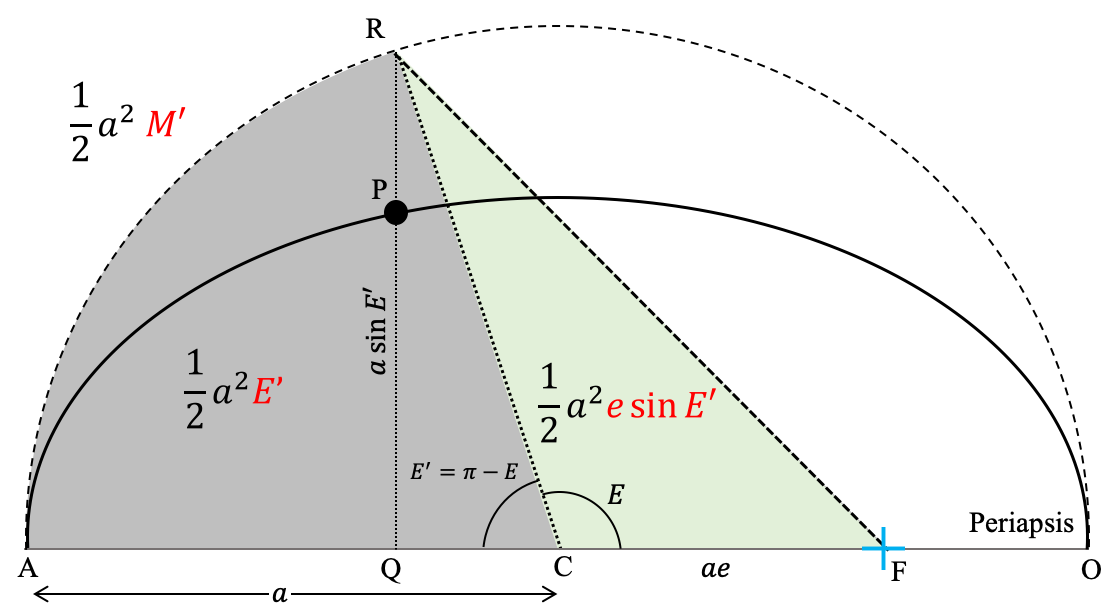
\includegraphics[width=1\textwidth]{./figures/horizontal_anomalia_media.png}
\caption{Construcción geométrica original de Johannes Kepler para
interpretar la anomalía media \(M\) o su suplemento \(M'\equiv=\pi-M\).
Según Kepler \(M'\) es proporcional al área total de la región FRA que,
a su vez la suma del area triangulo RCF, que es proporcional a
\(e\sin E'\) y el área del sector de círculo RCA, que es proporcional a
\(E'\).\label{fig:anomalia_excentrica}}
\end{figure}

Kepler interpreto geométricamente la Ec. (\ref{eq:ecuacion_kepler}) en
términos de las áreas de sectores sobre la elipse. Para entender su
argumento debemos primero definir los suplementos de la anomalía
excéntrica \(E'\equiv\pi-E\) y de la anomalía media \(M'\equiv\pi-M\).

En términos de estos suplementos la ecuación de Kepler (Ec.
\ref{eq:ecuacion_kepler}) se escribe:

\[
M'=E'+e\sin E'
\]

A medida que el cuerpo se mueve sobre la elipse, el valor de la anomalía
excéntrica \(E\) y de su suplemento \(E'\) cambian con una velocidad
variable (recordemos que por el teorema de áreas el cuerpo se mueve más
rápido cerca al periapsis O.)

Cuando el cuerpo se encuentra en el punto P, toda el área sombreada en
la \autoref{fig:anomalia_media} (que es la que le falta barrer al radio
dirigido del foco a la circunferencia circunscrita, antes de llegar al
afelio), será igual al área del triángulo RCF más el área del sector de
círculo RCA:

\[
A_\mathrm{RFA}=A_\mathrm{RCA}+A_\mathrm{RCF}
\]

Pero \(A_\mathrm{RCA}=a^2 E'/2\) (área de un sector circular) y
\(A_\mathrm{RCF}=a^2 e \sin E'/2\) (área de un triángulo), de modo que
reemplazando el área total del sector sombreado en la
\autoref{eq:anomalia_media} queda:

\begin{eqnarray}
\nonumber
A_\mathrm{RFA} & = & \frac{1}{2}a^2(E'+e\sin E')\\
\nonumber
               & = & \frac{1}{2}a^2 M' 
\end{eqnarray} donde en el último paso hemos usado la ecuación de Kepler
en términos de los suplementos.

Este último resultado llevo a Kepler a planetar el problema del cálculo
de la posición planetaria sobre una elipse como aquel en el que el
Astrónomo, que puede predecir con suma facilidad el valor de la anomalía
media \(M=n(t-t_p)\), debe encontrar el lugar geométrico del punto R
sobre la circunferencia circunscrita (y que esta justo arriba del punto
sobre la elipse buscado buscado), tal que el área RFA sea igual a
\(a^2M'/2\).

Dado que el punto F no está en el centro de la circunferencia
circunscrita, \(M\) no se puede interpretar como ningún ángulo en la
construcción de la \autoref{fig:anomalia_media}. Como consecuencia de
este hecho, y como lo reconoció Kepler desde aquel entonces, el problema
de encontrar \(E'\) dado un valor de \(M'\) es altamente no trivial. A
la fecha no se conoce ninguna solución geométrica al problema de Kepler,
es decir, no podemos encontrar la posición del punto R usando solamente
una regla y un compás.

En términos algebraicos la conclusión de Kepler es equivalente a
reconocer que en la ecuación:

\[
M=E-e\sin E
\] es imposible despejar algebraicamente \(E\). A este tipo de
ecuaciones se las conoce en matemáticas como \emph{ecuaciones
trascendentales}.

Esta conclusión es válida también en el caso de la ecuación de Kepler
para el movimiento sobre una hipérbola:

\[
M_h=e\sinh F - F
\]

Si queremos entonces resolver el problema de los dos cuerpos en el
tiempo, al menos cuando \(e\neq 1\) tenemos que encontrar una manera
\emph{aproximada} de resolver esta ecuación. Este será justamente el
tema de la siguiente sección. No sobra, sin embargo, hacer aquí una
última reflexión, con la que podemos cerrar el esfuerzo de este capítulo
para encontrar una solución al problema de los dos cuerpos.

A pesar de que logramos encontrar un número suficiente de cuadraturas
para el problema e incluso encontramos una cantidad geométrica que
depende de la posición y que cambia de forma predecible con el tiempo
(el área barrida por el radiovector), la solución completa del problema
de los dos cuerpos dependerá en últimas de resolver numéricamente una
ecuación trascendental. En conclusión, ni siquiera la versión más simple
del problema general de los N cuerpos admite una solución algebraica
cerrada. Sin embargo y como veremos en la
\autoref{solucion_kepler_series} es posible encontrar una solución
en términos de series de potencias uniformemente convergentes (funciones
analíticas), satisfaciendo así las condiciones al problema de los N
cuerpos formulado en el \autoref{problema_ncuerpos}.



\hypertarget{solucion_kepler_numerica}{%
\subsection{Solución numérica a la ecuación de
Kepler}\label{solucion_kepler_numerica}}

Casi que desde que se formuló la ecuación de Kepler para órbitas
elípticas en 1609, decenas, sino cientos de métodos distintos se han
inventado para resolver la ecuación con distintos niveles de precisión.
Estos métodos han evolucionado mucho recientemente (especialmente a
partir de las últimas décadas de los 1900) obedeciendo, de un lado, a
las exigencias de los vuelos espaciales y la astronomía de alta
precisión y del otro a la disposición de computadoras que pueden
calcular a gran velocidad el valor aproximado de series infinitas o
aplicar métodos iterativos, independientemente de su complejidad. Para
una revisión exhaustiva de los distintos métodos y sus propiedades
numéricas se invita al lector a revisar el libro de Peter Colwell
``\emph{Solving Kepler's equation over three centuries}''
\cite{Colwell1993Kepler} o en la literatura especializada, la excelente
serie de artículos publicados por Danby y Burkardt
\cite{Danby1983KeplerI},\cite{Danby1983KeplerII},\cite{Danby1983KeplerIII}
o el también reconocido trabajo de Odell \& Gooding
\cite{Odell1986Kepler}.

A continuación hacemos una síntesis de algunos de los métodos ideados en
los últimos 300 años para resolver la ecuación de Kepler y describimos
algunos algorítmos que serán útiles en lo sucesivo en este libro. Nos
concentraremos específicamente en ilustrar la solución a la ecuación de
Kepler en el caso de órbitas elípticas, que son también las de mayor
interés en astronomía e ingeniería aeroespacial. Sin embargo, la mayoría
de estos métodos se aplican también para el caso hiperbólico sin muchas
modificaciones.

Bajo ninguna circunstancia, esta breve síntesis puede considerarse
completa o representativa de la vasta literatura en el tema. Este
resumen, tiene el único propósito de poner al tanto al lector de algunos
los retos y de los logros matemáticos que se han conseguido en esta
materia durante el par de siglos que nos separan desde los trabajos
pioneros de Kepler.

\hypertarget{kepler_metodo_kepler}{%
\subsubsection{El Método de Kepler}\label{kepler_metodo_kepler}}

El primer método ideado para resolver la Ec. (\ref{eq:ecuacion_kepler})
fue presentado precisamente por el mismo Kepler en su libro "Epítome de
la astronomía Copernicana* publicado entre 1617 y 1621\footnote{En este
  libro apareció también formulada por primera vez la ley armónica, que
  llamamos aquí tercer teorema del movimiento orbital o teorema
  armónico. En los Epítome Kepler uso también por primera vez la palabra
  \emph{inercia}, cuyo concepto sería elaborado en profundidad
  posteriormente por Galileo, Descartes y por supuesto por Newton.}

Para ilustrar el método original de Kepler, supongamos que queremos
encontrar el valor de la anomalía excéntrica para los siguientes valores
de \(e\) y \(M\):

    \begin{code}{}{}\begin{Verbatim}[fontsize=\small,commandchars=\\\{\}]
\PY{n}{e}\PY{o}{=}\PY{l+m+mf}{0.5}
\PY{n}{M}\PY{o}{=}\PY{l+m+mi}{37} \PY{c+c1}{\PYZsh{}grados}
\end{Verbatim}

%%

\end{code}

El método consiste en elegir un valor para la anomalía excéntrica
\(E_0\), que sirva como punto de partida. Escojamos por ejemplo el
siguiente valor para esta cantidad:

    \begin{code}{}{}\begin{Verbatim}[fontsize=\small,commandchars=\\\{\}]
\PY{n}{E0}\PY{o}{=}\PY{l+m+mi}{45} 
\end{Verbatim}

%%

\end{code}

El siguiente paso consiste en calcular el valor de la anomalía media
\(M_0\) correspondiente a \(E_0\) de acuerdo con la ecuación de Kepler:

\[M_0=E_0-e\sin E_0\]

Para usar las funciones trigonométricas tenermos que convertir primero
los valores de \texttt{M} y \texttt{E0} a radianes:

    \begin{code}{}{}\begin{Verbatim}[fontsize=\small,commandchars=\\\{\}]
\PY{k+kn}{from} \PY{n+nn}{numpy} \PY{k}{import} \PY{n}{pi}
\PY{n}{M}\PY{o}{=}\PY{n}{M}\PY{o}{*}\PY{n}{pi}\PY{o}{/}\PY{l+m+mi}{180}
\PY{n}{E0}\PY{o}{=}\PY{n}{E0}\PY{o}{*}\PY{n}{pi}\PY{o}{/}\PY{l+m+mi}{180}

\PY{k+kn}{from} \PY{n+nn}{numpy} \PY{k}{import} \PY{n}{sin}
\PY{n}{M0}\PY{o}{=}\PY{n}{E0}\PY{o}{\PYZhy{}}\PY{n}{e}\PY{o}{*}\PY{n}{sin}\PY{p}{(}\PY{n}{E0}\PY{p}{)}
\end{Verbatim}

%%

\end{code}
\vspace{-1em}

%%hidecode


    \begin{Verbatim}[fontsize=\small,commandchars=\\\{\}]
M0 = 24.742882886465114 grados
\end{Verbatim}

Como vemos, \(M_0\) no coincide con el valor original de \(M\). Sin
embargo podemos usar la diferencia \(\epsilon_0=M-M_0\) para calcular un
valor corregido de la anomalía excéntrica, \(E_1=E_0+\epsilon_0\):

    \begin{code}{}{}\begin{Verbatim}[fontsize=\small,commandchars=\\\{\}]
\PY{n}{epsilon0}\PY{o}{=}\PY{n}{M}\PY{o}{\PYZhy{}}\PY{n}{M0}
\PY{n}{E1}\PY{o}{=}\PY{n}{E0}\PY{o}{+}\PY{n}{epsilon0}
\end{Verbatim}

%%

\end{code}
\vspace{-1em}

%%hidecode


    \begin{Verbatim}[fontsize=\small,commandchars=\\\{\}]
epsilon0 = 12.257117113534887
E1 = 57.25711711353489 grados
\end{Verbatim}

Si repetimos el procedimiento anterior podemos encontrar un tercer valor
para \(E\):

    \begin{code}{}{}\begin{Verbatim}[fontsize=\small,commandchars=\\\{\}]
\PY{n}{M1}\PY{o}{=}\PY{n}{E1}\PY{o}{\PYZhy{}}\PY{n}{e}\PY{o}{*}\PY{n}{sin}\PY{p}{(}\PY{n}{E1}\PY{p}{)}
\PY{n}{epsilon1}\PY{o}{=}\PY{n}{M}\PY{o}{\PYZhy{}}\PY{n}{M1}
\PY{n}{E2}\PY{o}{=}\PY{n}{E1}\PY{o}{+}\PY{n}{epsilon1}
\end{Verbatim}

%%

\end{code}
\vspace{-1em}

%%hidecode


    \begin{Verbatim}[fontsize=\small,commandchars=\\\{\}]
M1 = 33.16119928670333
epsilon1 = 3.8388007132966724
E2 = 61.09591782683156
\end{Verbatim}

Vemos que en esta segunda iteración, el valor de \(M_1\) es más cercano
al valor real de \(M\), lo que muestra que el procedimiento esta
\emph{convergiendo}. Si repetimos la misma \emph{regla de iteración}
otras 5 veces obtenemos la siguiente secuencia de valores de \(M\),
\(\epsilon\) y \(E\):
\vspace{-1em}

%%hidecode


    \begin{Verbatim}[fontsize=\small,commandchars=\\\{\}]
Paso 3: M2 = 36.02 gr., epsilon2 = 0.983 gr., E3 = 62.07922 gr.
Paso 4: M3 = 36.77 gr., epsilon3 = 0.234 gr., E4 = 62.31316 gr.
Paso 5: M4 = 36.95 gr., epsilon4 = 0.055 gr., E5 = 62.36772 gr.
Paso 6: M5 = 36.99 gr., epsilon5 = 0.013 gr., E6 = 62.38038 gr.
Paso 7: M6 = 37.00 gr., epsilon6 = 0.003 gr., E7 = 62.38332 gr.
\end{Verbatim}

Notamos que el valor de \(\epsilon\) se hace cada vez más pequeño y el
valor de la anomalía excéntrica se estabiliza con lo que podemos
asegurar que el valor real de esta cantidad esta cerca del último valor
de \(E\) presentado en la lista de arriba. El \emph{margen de error} de
nuestra estimación se puede cifrar cercano a \(\epsilon\).

En términos simbólicos la regla de iteración del método de Kepler se
puede escribir como:

\begin{equation}
\label{eq:kepler_kepler}
\begin{array}{rcl}
M_{n} & = & E_{n}-e\sin E_{n}\\
\epsilon_{n} & = & M-M_{n}\\
E_{n+1} & = & E_{n}+\epsilon_{n}
\end{array}
\end{equation} con \(n=0,1,2\ldots\).

El \emph{criterio de convergencia}, es decir la condición que nos
permite decir cuándo estamos satisfechos con el último valor de la
anomalía excéntrica provisto por la regla, puede definirse con la
condición:

\[
\Delta_n\equiv\left|\frac{\epsilon_n}{M}\right|<\delta
\] donde \(\Delta_n\) es una estimación del \emph{error relativo} del
algoritmo en el paso \(n\) y \(\delta\) es un número arbitrariamente
pequeño escogido por el usuario. Llamamos a \(\delta\) la
\emph{tolerancia solicitada}.

Como regla general, puede ser interesante tomar, en lugar del último
valor de la anomalía excéntrica provisto por el método iterativo, es
decir \(E_{n+1}\), el valor promedio entre los dos últimos \emph{pasos}:

\[
\bar{E}=\frac{E_n+E_{n+1}}{2}
\]

Finalmente el valor verdadero de la anomalía excéntrica estará contenido
con alta probabilidad en el intervalo:

\[
E\in[\bar{E}-2\Delta_n\bar E,\bar{E}+2\Delta_n\bar E]
\] que se puede escribir como:

\[
E=\bar{E}\pm \Delta_n\bar E
\]

El método de Kepler se puede implementar con la siguiente rutina:

    \begin{code}{Algoritmo}{code:kepler_kepler}\begin{Verbatim}[fontsize=\small,commandchars=\\\{\}]
\PY{k}{def} \PY{n+nf}{kepler\PYZus{}kepler}\PY{p}{(}\PY{n}{M}\PY{p}{,}\PY{n}{e}\PY{p}{,}\PY{n}{E0}\PY{o}{=}\PY{l+m+mf}{1.0}\PY{p}{,}\PY{n}{delta}\PY{o}{=}\PY{l+m+mf}{1e\PYZhy{}5}\PY{p}{)}\PY{p}{:}
    \PY{c+c1}{\PYZsh{}Valor inicial de la anomalía excéntrica}
    \PY{n}{E}\PY{o}{=}\PY{n}{E0}
    \PY{c+c1}{\PYZsh{}Valor inicial del error relativo}
    \PY{n}{Dn}\PY{o}{=}\PY{l+m+mi}{1}
    \PY{c+c1}{\PYZsh{}Contador de iteraciones}
    \PY{n}{ni}\PY{o}{=}\PY{l+m+mi}{0}
    \PY{k}{while} \PY{n}{Dn}\PY{o}{\PYZgt{}}\PY{n}{delta}\PY{p}{:}
        \PY{c+c1}{\PYZsh{}\PYZdq{}En\PYZdq{} es igual al último valor de E}
        \PY{n}{En}\PY{o}{=}\PY{n}{E}
        \PY{c+c1}{\PYZsh{}Regla de iteración}
        \PY{k+kn}{from} \PY{n+nn}{math} \PY{k}{import} \PY{n}{sin}
        \PY{n}{Mn}\PY{o}{=}\PY{n}{En}\PY{o}{\PYZhy{}}\PY{n}{e}\PY{o}{*}\PY{n}{sin}\PY{p}{(}\PY{n}{En}\PY{p}{)}
        \PY{n}{en}\PY{o}{=}\PY{n}{M}\PY{o}{\PYZhy{}}\PY{n}{Mn}
        \PY{n}{E}\PY{o}{=}\PY{n}{En}\PY{o}{+}\PY{n}{en}
        \PY{c+c1}{\PYZsh{}Valor promedio}
        \PY{n}{Emed}\PY{o}{=}\PY{p}{(}\PY{n}{E}\PY{o}{+}\PY{n}{En}\PY{p}{)}\PY{o}{/}\PY{l+m+mi}{2}
        \PY{c+c1}{\PYZsh{}Error relativo}
        \PY{n}{Dn}\PY{o}{=}\PY{n+nb}{abs}\PY{p}{(}\PY{n}{en}\PY{o}{/}\PY{n}{M}\PY{p}{)}
        \PY{c+c1}{\PYZsh{}Conteo de iteraciones}
        \PY{n}{ni}\PY{o}{+}\PY{o}{=}\PY{l+m+mi}{1}
    \PY{k}{return} \PY{n}{Emed}\PY{p}{,}\PY{n}{Dn}\PY{p}{,}\PY{n}{ni}
\end{Verbatim}

%%

\end{code}

Que se invoca como:

    \begin{code}{}{}\begin{Verbatim}[fontsize=\small,commandchars=\\\{\}]
\PY{n}{E}\PY{p}{,}\PY{n}{error}\PY{p}{,}\PY{n}{ni}\PY{o}{=}\PY{n}{kepler\PYZus{}kepler}\PY{p}{(}\PY{n}{M}\PY{p}{,}\PY{n}{e}\PY{p}{,}\PY{n}{E0}\PY{p}{,}\PY{l+m+mf}{1e\PYZhy{}8}\PY{p}{)}
\end{Verbatim}

%%

\end{code}
\vspace{-1em}

%%hidecode


    \begin{Verbatim}[fontsize=\small,commandchars=\\\{\}]
M = 37, e = 0.50
E estimada (promedio últimos dos pasos) = 62.38420178431245
Error absoluto = 1.1e-07 grados
Intervalo = [62.38420157333525,62.384201995289665] grados
Número de iteraciones: 14
\end{Verbatim}

\hypertarget{kepler_metodo_puntofijo}{%
\subsubsection{Método del punto fijo}\label{kepler_metodo_puntofijo}}

Otro método muy común y sencillo de entender e implementar es el método
del punto fijo. Este método parte de reescribir la ecuación de Kepler
como:

\[
E=M+e\sin E
\]

Escrita de esta manera la solución a la ecuación de Kepler es
equivalente a la búsqueda del punto de intersección entre la recta \(E\)
y la curva \(M-e\sin E\).

La regla de iteración del método del punto fijo es:

\begin{equation}
\label{eq:kepler_puntofijo}
\begin{array}{rcl}
E_{n+1} & = & M+e\sin E_n\\
\epsilon_n & = & E_{n+1}-E_n\\
\end{array}
\end{equation} con un criterio de convergencia:

\[
\left|\frac{\epsilon_n}{\bar{E}}\right|<\delta
\]

Es fácil mostrar que las ecuaciones de iteración del método original de
Kepler (Ecs. \ref{eq:kepler_kepler}) son equivalentes a las del método
del punto fijo (ver problemas al final del capítulo.)

\hypertarget{kepler_metodo_newton}{%
\subsubsection{Método de Newton-Raphson}\label{kepler_metodo_newton}}

Los métodos más rápidos que se han diseñado en la historia para resolver
numéricamente la ecuación de Kepler son variaciones de un método cuya
autoría original se atribuye a Newton. En 1669 en su ensayo ``Sobre el
análisis por series infinitas'' (que además se considera el primer texto
de cálculo infinitesimal de la historia) Newton presentó una versión
particular del método aplicado exclusivamente al caso de funciones
polinómicas. El método fue generalizado para funciones no polinómicas en
1690 por Joseph Raphson, razón por la cuál recibe hoy el nombre de
\textbf{método de Newton-Raphson}.

El método permite encontrar las raices de ecuaciones del tipo:

\[
f(x)=0
\] donde \(f(E)\) es una ecuación diferenciable al menos una vez.
Claramente la \textbf{función generalizada de Kepler}, que introdujimos
en la \autoref{funcion_kepler} (Ec. \ref{eq:kepler_generalizada}),
satisface esta condición.

La raiz de la ecuación se obtiene usando la regla de iteración:

\[
x_{n+1} = x_n-\frac{f(x_n)}{f'(x_n)}\\
\] con \(f'(x)=\mathrm{d}f/\mathrm{d}x\).

Si usamos la forma explícita de la función generalizada de Kepler y de
su primera derivada (Ec. \label{eq:kepler_generalizada_derivada1}) la
regla de iteración del método de Newton-Raphson aplicado al problema de
Kepler queda:

\[
G_{n+1} = \frac{M/\sigma+e\;\mathrm{s}G_n-e G_n\;\mathrm{c}G_n}{1-e\;\mathrm{c}G_n}
\]

Esta regla se puede implementar con la siguiente rutina:

    \begin{code}{Algoritmo}{code:kepler_newton}\begin{Verbatim}[fontsize=\small,commandchars=\\\{\}]
\PY{k}{def} \PY{n+nf}{kepler\PYZus{}newton}\PY{p}{(}\PY{n}{M}\PY{p}{,}\PY{n}{e}\PY{p}{,}\PY{n}{G0}\PY{o}{=}\PY{l+m+mi}{1}\PY{p}{,}\PY{n}{delta}\PY{o}{=}\PY{l+m+mf}{1e\PYZhy{}5}\PY{p}{)}\PY{p}{:}
    \PY{c+c1}{\PYZsh{}Valor inicial de la anomalía excéntrica}
    \PY{n}{Gn}\PY{o}{=}\PY{n}{G0}
    \PY{c+c1}{\PYZsh{}Valor inicial del error relativo}
    \PY{n}{Dn}\PY{o}{=}\PY{l+m+mi}{1}
    \PY{c+c1}{\PYZsh{}Contador de iteraciones}
    \PY{n}{ni}\PY{o}{=}\PY{l+m+mi}{0}
    \PY{k}{while} \PY{n}{Dn}\PY{o}{\PYZgt{}}\PY{n}{delta}\PY{p}{:}
        \PY{c+c1}{\PYZsh{}Inicializa el valor de En}
        \PY{n}{G}\PY{o}{=}\PY{n}{Gn}
        \PY{c+c1}{\PYZsh{}Función de Kepler y de su primera derivada en G}
        \PY{k+kn}{from} \PY{n+nn}{pymcel}\PY{n+nn}{.}\PY{n+nn}{export} \PY{k}{import} \PY{n}{funcion\PYZus{}kepler}
        \PY{n}{k}\PY{p}{,}\PY{n}{kp}\PY{p}{,}\PY{n}{kpp}\PY{o}{=}\PY{n}{funcion\PYZus{}kepler}\PY{p}{(}\PY{n}{G}\PY{p}{,}\PY{n}{M}\PY{p}{,}\PY{n}{e}\PY{p}{)}
        \PY{c+c1}{\PYZsh{}Nuevo valor (regla de iteración)}
        \PY{n}{Gn}\PY{o}{=}\PY{n}{G}\PY{o}{\PYZhy{}}\PY{n}{k}\PY{o}{/}\PY{n}{kp}
        \PY{c+c1}{\PYZsh{}Valor medio}
        \PY{n}{Gmed}\PY{o}{=}\PY{p}{(}\PY{n}{G}\PY{o}{+}\PY{n}{Gn}\PY{p}{)}\PY{o}{/}\PY{l+m+mi}{2}
        \PY{c+c1}{\PYZsh{}Criterio de convergencia}
        \PY{n}{en}\PY{o}{=}\PY{n}{Gn}\PY{o}{\PYZhy{}}\PY{n}{G}
        \PY{n}{Dn}\PY{o}{=}\PY{n+nb}{abs}\PY{p}{(}\PY{n}{en}\PY{o}{/}\PY{n}{Gmed}\PY{p}{)}
        \PY{n}{ni}\PY{o}{+}\PY{o}{=}\PY{l+m+mi}{1}
    \PY{k}{return} \PY{n}{Gmed}\PY{p}{,}\PY{n}{Dn}\PY{p}{,}\PY{n}{ni}
\end{Verbatim}

%%

\end{code}

Al aplicarlo al ejemplo anterior queda:

    \begin{code}{}{}\begin{Verbatim}[fontsize=\small,commandchars=\\\{\}]
\PY{n}{E}\PY{p}{,}\PY{n}{error}\PY{p}{,}\PY{n}{ni}\PY{o}{=}\PY{n}{kepler\PYZus{}newton}\PY{p}{(}\PY{n}{M}\PY{p}{,}\PY{n}{e}\PY{p}{,}\PY{n}{E0}\PY{p}{,}\PY{l+m+mf}{1e\PYZhy{}8}\PY{p}{)}
\end{Verbatim}

%%

\end{code}
\vspace{-1em}

%%hidecode


    \begin{Verbatim}[fontsize=\small,commandchars=\\\{\}]
M = 37, e = 0.50
E estimada (promedio últimos dos pasos) = 62.38420186888202
Error absoluto = 0.0e+00 grados
Intervalo = [62.38420186888202,62.38420186888202] grados
Número de iteraciones: 5
\end{Verbatim}

Que como se ve, converge muchísimo más rápido que el método de punto
fijo.

Una rutina general que aplica el método de Newton de forma análoga a
como lo hemos hecho en la rutina \texttt{kepler\_newton}, pero para
encontrar la raíz de cualquier función es provisto en el
\autoref{algoritmos_utiles}. Esta rutina será utilizada en el libro
con alguna frecuencia. Un ejemplo de su uso para el caso ilustrado aquí
se muestra a continuación:

    \begin{code}{}{}\begin{Verbatim}[fontsize=\small,commandchars=\\\{\}]
\PY{k+kn}{from} \PY{n+nn}{pymcel}\PY{n+nn}{.}\PY{n+nn}{export} \PY{k}{import} \PY{n}{funcion\PYZus{}kepler}\PY{p}{,}\PY{n}{metodo\PYZus{}newton}
\PY{n}{E}\PY{p}{,}\PY{n}{error}\PY{p}{,}\PY{n}{ni}\PY{o}{=}\PY{n}{metodo\PYZus{}newton}\PY{p}{(}\PY{n}{funcion\PYZus{}kepler}\PY{p}{,}\PY{n}{x0}\PY{o}{=}\PY{n}{E0}\PY{p}{,}\PY{n}{delta}\PY{o}{=}\PY{l+m+mf}{1e\PYZhy{}8}\PY{p}{,}\PY{n}{args}\PY{o}{=}\PY{p}{(}\PY{n}{M}\PY{p}{,}\PY{n}{e}\PY{p}{)}\PY{p}{)}
\end{Verbatim}

%%

\end{code}
\vspace{-1em}

%%hidecode


    \begin{Verbatim}[fontsize=\small,commandchars=\\\{\}]
M = 37, e = 0.50
E estimada (promedio últimos dos pasos) = 62.38420186888202
Error absoluto = 0.0e+00 grados
Intervalo = [62.38420186888202,62.38420186888202] grados
Número de iteraciones: 5
\end{Verbatim}

\hypertarget{kepler_laguerre}{%
\subsubsection{El método de Laguerre-Conway}\label{kepler_laguerre}}

Décadas de experimentación numérica han mostrado que el método de
Newton, si bien simple y poderoso, puede no converger con la precisión y
velocidad apropiadas para ciertos pares de valores de \(M\) y \(e\). Un
método con convergencia rápida y asegurada es el método de
Laguerre-Conway \cite{Conway1986} que usa la siguiente regla de
iteración:

\begin{eqnarray}
\epsilon_n & = & \frac{\eta f(x)}{f'(x_n)\pm\sqrt{(\eta-1)^2(f'(x_n))^2-\eta(\eta-1)f(x_n)f''(x_n)}} \\
E_{n+1} & = & E_n-\epsilon_n
\end{eqnarray} donde \(\eta\) es un parámetro entero. Cuando \(\eta=1\)
el método de Laguerre-Conway es equivalente al método de Newton.

Experimentos numéricos han mostrado que el valor óptimo de \(\eta\) en
el caso de la ecuación de Kepler es \(\eta=5\).

En el \autoref{algoritmos_utiles} el lector puede encontrar una
rutina general que aplica el método de Laguerre-Conway para encontrar la
raíz de cualquier ecuación. Un ejemplo de su uso para la ecuación de
Kepler se muestra a continuación:

    \begin{code}{}{}\begin{Verbatim}[fontsize=\small,commandchars=\\\{\}]
\PY{k+kn}{from} \PY{n+nn}{pymcel}\PY{n+nn}{.}\PY{n+nn}{export} \PY{k}{import} \PY{n}{funcion\PYZus{}kepler}\PY{p}{,}\PY{n}{metodo\PYZus{}laguerre}
\PY{n}{E}\PY{p}{,}\PY{n}{error}\PY{p}{,}\PY{n}{ni}\PY{o}{=}\PY{n}{metodo\PYZus{}laguerre}\PY{p}{(}\PY{n}{funcion\PYZus{}kepler}\PY{p}{,}\PY{n}{x0}\PY{o}{=}\PY{n}{E0}\PY{p}{,}\PY{n}{delta}\PY{o}{=}\PY{l+m+mf}{1e\PYZhy{}8}\PY{p}{,}\PY{n}{args}\PY{o}{=}\PY{p}{(}\PY{n}{M}\PY{p}{,}\PY{n}{e}\PY{p}{)}\PY{p}{)}
\end{Verbatim}

%%

\end{code}
\vspace{-1em}

%%hidecode


    \begin{Verbatim}[fontsize=\small,commandchars=\\\{\}]
M = 37, e = 0.50
E estimada (promedio últimos dos pasos) = 62.38420186756679
Error absoluto = 2.6e-09 grados
Intervalo = [62.38420186493632,62.384201870197266] grados
Número de iteraciones: 3
\end{Verbatim}

Nótese que el número de iteraciones es mucho menor que en el caso del
método de Newton.

\hypertarget{kepler_horquillado}{%
\subsubsection{Métodos de horquillado}\label{kepler_horquillado}}

En los métodos de Kepler, Newton-Raphson y Laguerre-Conway visto en las
secciones anteriores, es necesario proveerun primer valor inicial de la
anomalía excéntrica (la variable \texttt{E0} en los algoritmos
presentados hasta aquí.) Determinar el valor óptimo de \texttt{E0} ha
probado ser una tarea poco trivial. Existen métodos alternativos, que
aunque mucho menos eficientes, solo requieren conocer a priori un
intervalo en el que se encuentre la solución. En el análisis numérico a
estos métodos se los llama en general \emph{bracketing methods} o
``métodos de horquillado.'' En el paquete \texttt{optimize} de la
biblioteca \texttt{SciPy} podrán encontrar un conjunto de rutinas
generales que implementan métodos de horquillado para encontrar la raiz
de funciones trascendentales.

Para encontrar un intervalo de horquillado general, en el caso del
movimiento elíptico, comencemos con la ecuación de Kepler escrita de la
forma (Ec. \ref{eq:ecuacion_kepler}):

\[
e\sin E-E=-M
\]

Como sabemos que \(-1\leq\sin E\leq 1\), el término del lado izquierdo
de la ecuación estará acotado por \(-e-E\leq e\sin E-E\leq e-E\). De
allí, la ecuación de Kepler se puede escribir en forma de desigualdad:

\[
-e-E\leq -M\leq e-E
\] trasponiendo algunos términos encontramos que:

\[
M-e\leq E\leq M+e
\] que es el intervalo de horquillado deseado.

Para el caso hiperbólico la ecuación de Kepler tiene la forma (Ec.
\ref{eq:ecuacion_kepler_hiperbolica}):

\[
e\sinh F-F=M
\]

Usando la respresentación en series de Taylor de la función seno
hiperbólico:

\[
\sinh F=F+\frac{F^3}{3!}+\frac{F^5}{5!}+\ldots
\] vemos que \(\sinh F\) esta acotada por debajo por:

\[\sinh F\geq F\]

Sin embargo la función no tienen ninguna cota superior. Con esto, la
ecuación de Kepler hiperbólica se puede escribir en forma de desigualdad
como:

\[
M\geq (e-1)F
\] de donde obtenemos el límite superior de nuestro intervalo de
horquillado:

\[
F\leq\frac{M}{e-1}
\]

Ahora bien, sabemos que el mínimo valor de la anomalía excéntrica es
\(F=0\) cuando \(M=0\). Para todos los valores positivos de \(M\),
\(F\geq 0\). Con esto podemos finalmente escribir un intervalo de
horquillado completo para el caso hiperbólico como:

\[
0\leq F\leq \frac{M}{e-1}
\]

En el algoritmo abajo se ilustra el uso de algunas de los métodos de
horquillado implementados en \texttt{SciPy.optimize} para resolver la
ecuación de Kepler en el ejemplo desarrollado en esta sección:

    \begin{code}{}{}\begin{Verbatim}[fontsize=\small,commandchars=\\\{\}]
\PY{k+kn}{from} \PY{n+nn}{numpy} \PY{k}{import} \PY{n}{pi}
\PY{k+kn}{from} \PY{n+nn}{scipy} \PY{k}{import} \PY{n}{optimize}

\PY{c+c1}{\PYZsh{}Recuerde que funcion\PYZus{}kepler devuelve también las derivadas}
\PY{k+kn}{from} \PY{n+nn}{pymcel}\PY{n+nn}{.}\PY{n+nn}{export} \PY{k}{import} \PY{n}{funcion\PYZus{}kepler}
\PY{n}{kepler}\PY{o}{=}\PY{k}{lambda} \PY{n}{G}\PY{p}{,}\PY{n}{M}\PY{p}{,}\PY{n}{e}\PY{p}{:}\PY{n}{funcion\PYZus{}kepler}\PY{p}{(}\PY{n}{G}\PY{p}{,}\PY{n}{M}\PY{p}{,}\PY{n}{e}\PY{p}{)}\PY{p}{[}\PY{l+m+mi}{0}\PY{p}{]}

\PY{c+c1}{\PYZsh{}Método de bisección}
\PY{n}{E\PYZus{}bis}\PY{p}{,}\PY{n}{info\PYZus{}bis}\PY{o}{=}\PY{n}{optimize}\PY{o}{.}\PY{n}{bisect}\PY{p}{(}\PY{n}{kepler}\PY{p}{,}\PY{n}{M}\PY{o}{\PYZhy{}}\PY{n}{e}\PY{p}{,}\PY{n}{M}\PY{o}{+}\PY{n}{e}\PY{p}{,}\PY{n}{rtol}\PY{o}{=}\PY{l+m+mf}{1e\PYZhy{}8}\PY{p}{,}
                               \PY{n}{args}\PY{o}{=}\PY{p}{(}\PY{n}{M}\PY{p}{,}\PY{n}{e}\PY{p}{)}\PY{p}{,}\PY{n}{full\PYZus{}output}\PY{o}{=}\PY{k+kc}{True}\PY{p}{)}
\PY{n}{ni\PYZus{}bis}\PY{o}{=}\PY{n}{info\PYZus{}bis}\PY{o}{.}\PY{n}{iterations}

\PY{c+c1}{\PYZsh{}Método de Brent}
\PY{n}{E\PYZus{}bre}\PY{p}{,}\PY{n}{info\PYZus{}bre}\PY{o}{=}\PY{n}{optimize}\PY{o}{.}\PY{n}{brentq}\PY{p}{(}\PY{n}{kepler}\PY{p}{,}\PY{n}{M}\PY{o}{\PYZhy{}}\PY{n}{e}\PY{p}{,}\PY{n}{M}\PY{o}{+}\PY{n}{e}\PY{p}{,}\PY{n}{rtol}\PY{o}{=}\PY{l+m+mf}{1e\PYZhy{}8}\PY{p}{,}
                               \PY{n}{args}\PY{o}{=}\PY{p}{(}\PY{n}{M}\PY{p}{,}\PY{n}{e}\PY{p}{)}\PY{p}{,}\PY{n}{full\PYZus{}output}\PY{o}{=}\PY{k+kc}{True}\PY{p}{)}
\PY{n}{ni\PYZus{}bre}\PY{o}{=}\PY{n}{info\PYZus{}bre}\PY{o}{.}\PY{n}{iterations}

\PY{c+c1}{\PYZsh{}Método de Ridder}
\PY{n}{E\PYZus{}rid}\PY{p}{,}\PY{n}{info\PYZus{}rid}\PY{o}{=}\PY{n}{optimize}\PY{o}{.}\PY{n}{ridder}\PY{p}{(}\PY{n}{kepler}\PY{p}{,}\PY{n}{M}\PY{o}{\PYZhy{}}\PY{n}{e}\PY{p}{,}\PY{n}{M}\PY{o}{+}\PY{n}{e}\PY{p}{,}\PY{n}{rtol}\PY{o}{=}\PY{l+m+mf}{1e\PYZhy{}8}\PY{p}{,}
                               \PY{n}{args}\PY{o}{=}\PY{p}{(}\PY{n}{M}\PY{p}{,}\PY{n}{e}\PY{p}{)}\PY{p}{,}\PY{n}{full\PYZus{}output}\PY{o}{=}\PY{k+kc}{True}\PY{p}{)}
\PY{n}{ni\PYZus{}rid}\PY{o}{=}\PY{n}{info\PYZus{}rid}\PY{o}{.}\PY{n}{iterations}
\end{Verbatim}

%%

\end{code}
\vspace{-1em}

%%hidecode


    \begin{Verbatim}[fontsize=\small,commandchars=\\\{\}]
M = 37, e = 0.50
Bisección: E = 62.38420210930057408 iteraciones = 27
Brent: E = 62.38420186878084195 iteraciones = 6
Ridder: E = 62.38420218086032065 iteraciones = 4
\end{Verbatim}

\hypertarget{kepler_otros_metodos}{%
\subsubsection{Otros métodos}\label{kepler_otros_metodos}}

Otro esfuerzo notable realizado especialmente en las últimas décadas
\cite{Nijenhuis1991Kepler}, \cite{Fukushima1991Kepler} ha sido el de
desarrollar rutinas que resuelven la ecuación de Kepler ejecutando el
mínimo número de funciones analíticas (p.e. funciones trigonométricas) o
usando únicamente operaciones básicas (multiplicaciones, sumas,
divisiones).

En el \autoref{algoritmos_utiles} hemos incluido algunas rutinas que
se encuentran en la literatura y que usan esta aproximación.

Un ejemplo de ellas es la rutina \texttt{kepler\_semianalitico}
\cite{Nijenhuis1991Kepler}. Esta rutina cálcula el valor aproximado de
la anomalía excéntrica \(E\) usando un solo llamado de las funciones
seno y coseno. En comparación la rutina \texttt{kepler\_newton} (Alg.
\ref{code:kepler_newton}) en cada iteración usa 3 llamados a las
funciones trigonométricas, de modo que cuando, por ejemplo se quiere
obtener un valor de \(E\) con una precisión muy alta y el número de
iteraciones es también alto, gran parte del tiempo de computo se ha
invertido en calcular decenas de funciones trigonométricas.

Un ejemplo del uso de la rutina se muestra a continuación:

    \begin{code}{}{}\begin{Verbatim}[fontsize=\small,commandchars=\\\{\}]
\PY{k+kn}{from} \PY{n+nn}{pymcel}\PY{n+nn}{.}\PY{n+nn}{export} \PY{k}{import} \PY{n}{kepler\PYZus{}semianalitico}
\PY{n}{E}\PY{p}{,}\PY{n}{error}\PY{p}{,}\PY{n}{ni}\PY{o}{=}\PY{n}{kepler\PYZus{}semianalitico}\PY{p}{(}\PY{n}{M}\PY{p}{,}\PY{n}{e}\PY{p}{)}
\end{Verbatim}

%%

\end{code}
\vspace{-1em}

%%hidecode


    \begin{Verbatim}[fontsize=\small,commandchars=\\\{\}]
M = 37, e = 0.50
E estimada (promedio últimos dos pasos) = 62.38761309530199
Error absoluto = 4.4e-03 grados
Intervalo = [62.38319428043351,62.392031910170466] grados
Número de iteraciones: 1
\end{Verbatim}

A diferencia de los métodos iterativos vistos antes, la rutina
\texttt{kepler\_semianalitico} no permite calcular el valor de \(E\) con
una precisión arbitraria. Por el contrario, para cada valor de \(e\) y
\(M\) existe un único valor devuelto por la rutina y que difiere del
valor real en una cantidad que no puede predecirse con anticipación. Aún
así la rutina es suficientemente buena al menos para situaciones en las
que no se requiere una excesiva precisión, tal y como se evidencia en la
\autoref{fig:code:precision_seminalitica}. Como vemos allí el error
relativo \(\Delta_n=|E-\bar E|/E\) oscila entre \(\sim 0.01\) (para
valores de la excentricidad \(e>0.2\)) y \(\sim 10^{-12}\) (para bajas
excentricidades y algunos valores específicos de \(M\).
%%HIDE%%\vspace{-1em}

%%figcaption::hide::Errores de la rutina semianalítica, es decir, aquella que resuelve la ecuación de Kepler sin usar iteraciones y solo hace un llamado a las funciones trigonométricas.

%%hidecode


    \begin{center}

\begin{figure}[ht!]
\centering
    \adjustimage{max size={0.8\linewidth}{0.8\paperheight}}{combined_files/combined_1441_0.png}
\caption{Errores de la rutina semianalítica, es decir, aquella que resuelve la ecuación de Kepler sin usar iteraciones y solo hace un llamado a las funciones trigonométricas.\label{fig:hide}}
\end{figure}

    \end{center}
%{ \hspace*{\fill} \\}
    
Podemos usar \texttt{kepler\_semianalitico} (pero también cualquiera de
las rutinas vistas hasta aquí) para visualizar cómo varía la anomalía
excéntrica como función de la anomalía media, para distintos valores de
la excentridad. Para ello, en la \autoref{fig:code:E_vs_M} hemos
graficado el valor de la función \(g(M)=E(M)-M\).
\vspace{-1em}

%%figcaption::hide::Anomalía excéntrica como función de la anomalía verdadera para distintos valores de la excentricidad.

%%hidecode


    \begin{center}

\begin{figure}[ht!]
\centering
    \adjustimage{max size={0.8\linewidth}{0.8\paperheight}}{combined_files/combined_1443_0.png}
\caption{Anomalía excéntrica como función de la anomalía verdadera para distintos valores de la excentricidad.\label{fig:hide}}
\end{figure}

    \end{center}
%{ \hspace*{\fill} \\}
    
De allí podemos comprobar varias propiedades que convendrá mantener
presentes en la solución de problemas prácticos en mecánica celeste:

\begin{itemize}
\item
  El valor de \(E\) coincide con el de \(M\) cuando \(M=0,\pi,2\pi\). En
  términos de \(g(M)\), esto implica que \(g(0)=g(\pi)=g(2\pi)=0\).
  Llamamos a estos valores los \emph{puntos nodales} de \(g\).
\item
  La funcion \(g(M)\) es periódica en el intervalo \([0,2\pi)\) y
  antisimétrica alrededor de \(M=\pi\). Esto implica que para encontrar
  la solución a la ecuación de Kepler para cualquier valor de \(M\),
  basta encontrar el valor correspondiente en el intervalo \([0,\pi]\) y
  aplicar las reglas de antisimetría correspondientes. En términos
  matemáticos, para cualquier valor de \(M>\pi\):

  \[
  g(M)=-g(2\pi-M)
  \]
\item
  Para valores pequeños de \(e\), el valor de \(E\approx M\).
\item
  La máximas diferencias entre \(E\) y \(M\), para valores de
  \(e\approx 1\), se producen cuando \(M\approx 35^\circ\) y
  \(E\approx 90^\circ\).
\end{itemize}

\hypertarget{solucion_kepler_aproximacions}{%
\subsection{Solución analítica por aproximaciones
sucesivas}\label{solucion_kepler_aproximacions}}

La solución numérica a la ecuación de Kepler es una estrategia adecuada
cuando se trata de resolver problemas prácticos (predecir la posición de
un asteroide, calcular efemérides de los planetas, etc.) Sin embargo en
situaciones teóricas más generales, en las que la solución a la ecuación
es parte de algún desarrollo matemático, es poco lo que algoritmos
iterativos nos pueden enseñar.

Para subsanar esta limitación, casi desde el tiempo de Newton se han
encontrado soluciones a la ecuación expresadas como sumas parciales o
series infinitas (ver \autoref{series_infinitas}), que en el caso de
valores pequeños de la excentricidad proveen expresiones algebraicas
aproximadas para la anomalía excéntrica (y otras cantides de interés.)

Una de las más conocidas representaciones en series de la anomalía
excéntrica, puede obtenerse aplicando sucesivamente el método del punto
fijo (Ec. \ref{eq:kepler_punto_fijo}):

\begin{equation}
\label{eq:E_iteracion}
E_{n+1}=M+e\sin E_{n}
\end{equation}

Si hacemos \(E_0 = M\) y calculamos analíticamente el valor de las
primeras dos aproximaciones obtenemos:

\begin{eqnarray}
\label{eq:E_e1}
E_1 & = & M+e\sin M \\
\nonumber
E_2 & = & M+e\sin (M+e\sin M)
\end{eqnarray}

Aplicando las identidades de suma de ángulos en la última expresión,
podemos escribir:

\begin{equation}
\label{eq:E2}
\begin{array}{rcl}
E_2 & = & M+e\sin (M+e\sin M) \\
    & = & M + e[\sin M \cos (e\sin M) + \sin (e\sin M)\cos M]
\end{array}
\end{equation}

Las funciones trigonométricas en esta ecuación que tienen como argumento
la cantidad \(e\sin M<1\), pueden aproximarse usando las series de
Taylor de \(\cos\) y \(\sin\) (Ecs. \ref{eq:sin_taylor} y
\ref{eq:cos_taylor}):

\begin{eqnarray}
\label{eq:cos_taylor}
\cos t & = & 1-\frac{t^2}{2!} + \frac{t^4}{4!} +\ldots\\
\label{eq:sin_taylor}
\sin t & = & t-\frac{t^3}{3!} + \frac{t^5}{5!} +\ldots
\end{eqnarray}

Usando estas representaciones de las funciones trigonométricas y
truncando los términos proporcionales a \(e^3\) o potencias superiores
de \(e\), el valor de \(E_2\) en la Ec. (\ref{eq:E2}) se puede escribir
como:

\begin{equation}
\label{eq:E_e2}
E_2 \approx M + e\sin M + \frac{1}{2}e^2 \sin 2M
\end{equation}

El subíndice 2 en esta expresión entonces ya no solo representa el hecho
de que se trata de la segunda iteración en el método de punto fijo, sino
también de que esta expresión puede darnos el valor aproximado de la
excentricidad con un error proporcional a \(e^3\). Es decir, si la
escentricidad es suficientemente pequeña \(e\ll 1\) la Ec.
(\ref{eq:E_e2}) ofrecerá una aproximación bastante buena para la
anomalía excéntrica.

Si continuamos el proceso con una nueva iteración de la Ec.
(\ref{eq:E_iteracion}), pero usamos la expresión aproximada de \(E_2\)
obtenida en la Ec. (\ref{eq:E_e2}) obtenemos:

\[
E_3 = M + e\sin \left(M + e\sin M + \frac{1}{2}e^2 \sin 2M \right)
\]

Aplicando nuevamente la identidades del seno de suma de ángulos y
expandiendo las funciones trigonométricas compuestas hasta términos de
orden \(e^3\) (truncando todos los términos de orden \(e^4\) y
superiores) obtenemos una nueva aproximación:

\begin{equation}
\label{eq:E_e3}
E_3 \approx M + \left(e - \frac{1}{8}e^3 \right)\sin M + \frac{1}{2}e^2\sin 2M + \frac{3}{8}e^3\sin 3M
\end{equation}

La siguiente rutina permite calcular las aproximaciones provistas aquí:

    \begin{code}{Algoritmo}{code:kepler_aproximacion}\begin{Verbatim}[fontsize=\small,commandchars=\\\{\}]
\PY{k}{def} \PY{n+nf}{kepler\PYZus{}aproximacion}\PY{p}{(}\PY{n}{M}\PY{p}{,}\PY{n}{e}\PY{p}{,}\PY{n}{orden}\PY{o}{=}\PY{l+m+mi}{1}\PY{p}{)}\PY{p}{:}
    \PY{k+kn}{from} \PY{n+nn}{math} \PY{k}{import} \PY{n}{sin}
    
    \PY{c+c1}{\PYZsh{}Formula de acuerdo al orden de aproximacion}
    \PY{k}{if} \PY{n}{orden}\PY{o}{==}\PY{l+m+mi}{1}\PY{p}{:}
        \PY{n}{E}\PY{o}{=}\PY{n}{M}\PY{o}{+}\PY{n}{e}\PY{o}{*}\PY{n}{sin}\PY{p}{(}\PY{n}{M}\PY{p}{)}
    \PY{k}{elif} \PY{n}{orden}\PY{o}{==}\PY{l+m+mi}{2}\PY{p}{:}
        \PY{n}{E}\PY{o}{=}\PY{n}{M}\PY{o}{+}\PY{n}{e}\PY{o}{*}\PY{n}{sin}\PY{p}{(}\PY{n}{M}\PY{p}{)}\PY{o}{+}\PY{l+m+mf}{0.5}\PY{o}{*}\PY{n}{e}\PY{o}{*}\PY{o}{*}\PY{l+m+mi}{2}\PY{o}{*}\PY{n}{sin}\PY{p}{(}\PY{l+m+mi}{2}\PY{o}{*}\PY{n}{M}\PY{p}{)}
    \PY{k}{elif} \PY{n}{orden}\PY{o}{==}\PY{l+m+mi}{3}\PY{p}{:}
        \PY{n}{E}\PY{o}{=}\PY{n}{M}\PY{o}{+}\PY{p}{(}\PY{n}{e}\PY{o}{\PYZhy{}}\PY{l+m+mf}{1.}\PY{o}{/}\PY{l+m+mi}{8}\PY{o}{*}\PY{n}{e}\PY{o}{*}\PY{o}{*}\PY{l+m+mi}{3}\PY{p}{)}\PY{o}{*}\PY{n}{sin}\PY{p}{(}\PY{n}{M}\PY{p}{)}\PY{o}{+}\PY{l+m+mf}{0.5}\PY{o}{*}\PY{n}{e}\PY{o}{*}\PY{o}{*}\PY{l+m+mi}{2}\PY{o}{*}\PY{n}{sin}\PY{p}{(}\PY{l+m+mi}{2}\PY{o}{*}\PY{n}{M}\PY{p}{)}\PY{o}{+}\PY{l+m+mf}{3.}\PY{o}{/}\PY{l+m+mi}{8}\PY{o}{*}\PY{n}{e}\PY{o}{*}\PY{o}{*}\PY{l+m+mi}{3}\PY{o}{*}\PY{n}{sin}\PY{p}{(}\PY{l+m+mi}{3}\PY{o}{*}\PY{n}{M}\PY{p}{)}
        
    \PY{c+c1}{\PYZsh{}Estimación el error relativo}
    \PY{n}{Ma}\PY{o}{=}\PY{n}{E}\PY{o}{\PYZhy{}}\PY{n}{e}\PY{o}{*}\PY{n}{sin}\PY{p}{(}\PY{n}{E}\PY{p}{)}
    \PY{n}{Dn}\PY{o}{=}\PY{n+nb}{abs}\PY{p}{(}\PY{n}{Ma}\PY{o}{\PYZhy{}}\PY{n}{M}\PY{p}{)}\PY{o}{/}\PY{n}{M}
    
    \PY{k}{return} \PY{n}{E}\PY{p}{,}\PY{n}{Dn}\PY{p}{,}\PY{l+m+mi}{1}
\end{Verbatim}

%%

\end{code}

Un ejemplo de uso de la rutina se muestra en este algoritmo:

    \begin{code}{}{}\begin{Verbatim}[fontsize=\small,commandchars=\\\{\}]
\PY{n}{E1}\PY{p}{,}\PY{n}{error1}\PY{p}{,}\PY{n}{ni1}\PY{o}{=}\PY{n}{kepler\PYZus{}aproximacion}\PY{p}{(}\PY{n}{M}\PY{p}{,}\PY{n}{e}\PY{p}{,}\PY{n}{orden}\PY{o}{=}\PY{l+m+mi}{1}\PY{p}{)}
\PY{n}{E2}\PY{p}{,}\PY{n}{error2}\PY{p}{,}\PY{n}{ni1}\PY{o}{=}\PY{n}{kepler\PYZus{}aproximacion}\PY{p}{(}\PY{n}{M}\PY{p}{,}\PY{n}{e}\PY{p}{,}\PY{n}{orden}\PY{o}{=}\PY{l+m+mi}{2}\PY{p}{)}
\PY{n}{E3}\PY{p}{,}\PY{n}{error3}\PY{p}{,}\PY{n}{ni1}\PY{o}{=}\PY{n}{kepler\PYZus{}aproximacion}\PY{p}{(}\PY{n}{M}\PY{p}{,}\PY{n}{e}\PY{p}{,}\PY{n}{orden}\PY{o}{=}\PY{l+m+mi}{3}\PY{p}{)}
\end{Verbatim}

%%

\end{code}
\vspace{-1em}

%%hidecode


    \begin{Verbatim}[fontsize=\small,commandchars=\\\{\}]
M = 37, e = 0.50
E (orden e) = 54.2407304 (error 6.006443353743711)
E (orden e\^{}2) = 61.1252602 (error 0.9610525147400825)
E (orden e\^{}3) = 63.0938414 (error 0.5471173899178785)
\end{Verbatim}

En el \autoref{algoritmos_utiles} hemos incluído una rutina,
\texttt{kepler\_eserie}, que permite calcular la anomalía excéntrica
usando términos hasta un orden arbitrario \(e^n\). Un ejemplo del uso de
la rutina se presenta a continuación

    \begin{code}{}{}\begin{Verbatim}[fontsize=\small,commandchars=\\\{\}]
\PY{k+kn}{from} \PY{n+nn}{pymcel}\PY{n+nn}{.}\PY{n+nn}{export} \PY{k}{import} \PY{n}{kepler\PYZus{}eserie}
\PY{n}{E8}\PY{p}{,}\PY{n}{error8}\PY{p}{,}\PY{n}{ni1}\PY{o}{=}\PY{n}{kepler\PYZus{}eserie}\PY{p}{(}\PY{n}{M}\PY{p}{,}\PY{n}{e}\PY{p}{,}\PY{n}{orden}\PY{o}{=}\PY{l+m+mi}{8}\PY{p}{)}
\end{Verbatim}

%%

\end{code}
\vspace{-1em}

%%hidecode


    \begin{Verbatim}[fontsize=\small,commandchars=\\\{\}]
M = 37, e = 0.50
E (orden e\^{}8) = 62.3103928 (error 0.003867448222173536)
\end{Verbatim}

Esta rutina puede usarse de la misma manera que hemos usado otras
anteriormente, proveyendo el valor de la tolerancia con la que se quiere
encontrar la anomalía excéntrica:

    \begin{code}{}{}\begin{Verbatim}[fontsize=\small,commandchars=\\\{\}]
\PY{n}{E}\PY{p}{,}\PY{n}{error}\PY{p}{,}\PY{n}{ni}\PY{o}{=}\PY{n}{kepler\PYZus{}eserie}\PY{p}{(}\PY{n}{M}\PY{p}{,}\PY{n}{e}\PY{p}{,}\PY{l+m+mf}{1e\PYZhy{}8}\PY{p}{)}
\end{Verbatim}

%%

\end{code}
\vspace{-1em}

%%hidecode


    \begin{Verbatim}[fontsize=\small,commandchars=\\\{\}]
M = 37, e = 0.50
E estimada (promedio últimos dos pasos) = 62.38420069661132
Error absoluto = 3.1e-07 grados
Intervalo = [62.38420038384044,62.38420100938219] grados
Número de iteraciones: 32
\end{Verbatim}

El cálculo numérico de la anomalía excéntrica con esta serie de
aproximaciones sucesivas no es sin embargo muy eficiente y solo converge
cuando \(e<0.6\) (ver \autoref{algoritmos_utiles}.)

\hypertarget{solucion_kepler_series}{%
\subsection{Solución por series de la ecuación de
Kepler}\label{solucion_kepler_series}}

En la solución a la ecuación de Kepler discutida en la sección anterior,
vimos que al usar aproximaciones sucesivas, la anomalía excéntrica se
puede escribir en la forma:

\[
g(M)=E-M=B_1(e)\sin(M)+B_2(e)\sin(2M)+B_3(e)\sin(3M)+\ldots
\] donde \(B_1\), \(B_2\), \(B_3\), \ldots{} son funciones de la
excentricidad que deben encontrarse con los procedimientos vistos.

El hecho de que este procedimiento pueda extenderse indefinidamente nos
conduce naturalmente a suponer que la función \(g(M)\) puede escribirse
en general como la serie infinita:

\begin{equation}
\label{eq:serie_gM}
g(M)=\sum_{n=1}^{\infty} B_n(e)\sin(nM)
\end{equation} es decir como una serie de Fourier.

Como vimos en la \autoref{series_infinitas} los coeficiente \(B_n\)
de la serie en la Ec. (\ref{eq:serie_gM}) se pueden calcular usando:

\[
B_n=\frac{1}{\pi}\int_0^{2\pi} g(M)\sin(nM)\;\mathrm{d}M
\]

Si tenemos en cuenta las propiedades de simetría de \(g(M)\), a saber
\(g(M>\pi)=-g(2\pi-M)\), la integral anterior se puede escribir como:

\[
B_n=\frac{1}{\pi}\left[\int_0^{\pi} g(M)\sin(nM)\;\mathrm{d}M-\int_\pi^{2\pi} g(2\pi-M)\sin(nM)\;\mathrm{d}M\right]
\] que después de un cambio de variable \(M'=2\pi-M\) en la segunda
integral entre corchetes, conduce a la integral más sencilla:

\[
B_n=\frac{2}{\pi}\int_0^{\pi} g(M)\sin(nM)
\]

Integrando por partes con \(u=g(M)\) y \(dv=sin(nM)\;\mathrm{d}M\)
obtenemos:

\[
B_n=\frac{2}{n\pi}\left\{\left[-g(M)\cos(nM)\right]_0^{\pi}+\int_0^{\pi} \cos(nM)\mathrm{d}g\right\}
\]

Teniendo en cuenta que \(g(0)=g(\pi)=0\) (ver
\autoref{fig:code:E_vs_M}), \(\mathrm{d}g=\mathrm{d}E\) y
\(M=E-e\sin E\), el coeficiente \(A_n\) se puede escribir como:

\begin{equation}
\label{eq:An}
B_n=\frac{2}{n}\left[\frac{1}{\pi}\int_0^\pi \cos(nE-ne\sin E)\;\mathrm{d}E\right]
\end{equation}
\begin{box_history}{Un poco de historia}{}{nofloat}
\small

\textbf{Las funciones de Bessel y la ecuación de Kepler.} La importancia
de la función entre corchetes en la Ec. \ref{eq:An} fue reconocida por
primera vez por Friederich Wilhelm Bessel
(\hreffoot{https://forvo.com/search/Friedrich\%20Wilhelm\%20Bessel/de/}{``Fridrich
Vilhelm Besel''}) en 1826. En un artículo histórico que publico ese
mismo año, Bessel introdujo por primera vez la definición:

\begin{equation}
  \label{eq:Jn_integral}
  J_n(x)\equiv\frac{1}{\pi}\int_0^{\pi} \cos(n\theta-x\sin \theta)\;\mathrm{d}\theta
  \end{equation}

y llamo a estas funciones \emph{Funciones de Bessel}.

En el mismo artículo, Bessel demostró que estas funciones pueden
expresarse como series de Taylor en la forma:

\begin{equation}
  \label{eq:Jn_serie}
  J_n(x) = \sum_{k=0}^{\infty} \frac{(-1)^k}{(n+k)! k!}\left(\frac{x}{2} \right)^{n+2k}
  \end{equation}

y mostró adicionalmente que satisfacen una ecuación diferencial
característica, conocida hoy también como la \emph{ecuación diferencial
de Bessel}.

Hoy sabemos que estas funciones eran ya conocidas, al menos en la forma
de series de potencias desde 1703 por Johan Bernoulli y después fueron
aplicadas en 1764 por Leonhard Euler en sus estudios sobre las
vibraciones.

Es sin embargo notable, descubrir que fueron escritas por primera vez
por Bessel en relación con un problema de Mecánica Celeste.

\end{box_history}
Finalmente la solución a la ecuación de Kepler se puede escribir en
forma de la serie infinita:

\begin{equation}
\label{eq:kepler_bessel}
E = M + \sum_{n=1}^{\infty} \frac{2}{n}J_n(ne)\sin (nM)
\end{equation} donde \(J_n\) son las funciones de Bessel de \emph{primer
tipo} (Ecs. \ref{eq:Jn_integral} y \ref{eq:Jn_serie}) y a las cantidad
\(J_n(ne)\) se las conoce en mecánica celeste como \emph{coeficiente de
Bessel}.

Es importante anotar que esta serie converge para cualquier valor de
\(e<1\).

En el \autoref{algoritmos_utiles} encontrarán el algoritmo de la
rutina \texttt{kepler\_bessel(M,e,delta)} que implementa la Ec.
(\ref{eq:kepler_bessel}). Un ejemplo de uso se muestra en el algoritmo a
continuación

    \begin{code}{}{}\begin{Verbatim}[fontsize=\small,commandchars=\\\{\}]
\PY{k+kn}{from} \PY{n+nn}{pymcel}\PY{n+nn}{.}\PY{n+nn}{export} \PY{k}{import} \PY{n}{kepler\PYZus{}bessel}
\PY{n}{E}\PY{p}{,}\PY{n}{error}\PY{p}{,}\PY{n}{n}\PY{o}{=}\PY{n}{kepler\PYZus{}bessel}\PY{p}{(}\PY{n}{M}\PY{p}{,}\PY{n}{e}\PY{p}{,}\PY{l+m+mf}{1e\PYZhy{}8}\PY{p}{)}
\end{Verbatim}

%%

\end{code}
\vspace{-1em}

%%hidecode


    \begin{Verbatim}[fontsize=\small,commandchars=\\\{\}]
M = 37, e = 0.50
E estimada (promedio últimos dos pasos) = 62.38420129936800
Error absoluto = 8.0e-08 grados
Intervalo = [62.38420121961613,62.38420137911987] grados
Número de iteraciones: 32
\end{Verbatim}

Nótese que los métodos de las aproximaciones sucesivas visto en la
sección anterior como el de la serie de Fourier visto aquí, proveen
aproximaciones analíticas muy útiles para la teoría, pero, como ha
quedado demostrado en los algortimos en los que los implementamos, su
eficiencia numérica es muy inferior a la de los métodos iterativos
vistos en la \autoref{solucion_kepler_numerica}.

\hypertarget{kepler_precision_eficiencia}{%
\subsection{Eficiencia de los métodos de
solución}\label{kepler_precision_eficiencia}}

En las libretas que encontrará con la
\hreffoot{http://seap-udea.org/MecanicaCeleste_Zuluaga}{versión electrónica
del libro} encontrará algoritmos que permiten evaluar el tiempo de
ejecución y comparar la eficiencia de los distintos métodos numéricos
presentados aquí.



\hypertarget{doscuerpos_sintesis}{%
\section{Una síntesis del problema de los dos
cuerpos}\label{doscuerpos_sintesis}}

En las secciones anteriores hemos demostrado que es posible resolver
analíticamente el problema de los dos cuerpos, que podemos formular en
términos generales como:

\begin{quote}
\emph{Dadas las posiciones y velocidades de dos partículas en un tiempo
de referencia dado \(t_0\),
\({\vec x}_1(t_0):[{\vec r}_1(t_0)\;\dot{\vec r}_1(t_0)]\),
\({\vec x}_2(t_0):[{\vec r}_2(t_0)\;\dot{\vec r}_2(t_0)]\), calcular las
posiciones y velocidades de las partículas en cualquier instante de
tiempo pasado o futuro \(t\)}.
\end{quote}

Podríamos resumir la solución encontrada en este capítulo, con el
siguiente conjunto de operaciones o pasos, que partiendo de los vectores
de estado inicial \({\vec x}_1(t_0)\), \({\vec x}_2(t_0)\), nos permiten
obtener los vectores de estado \({\vec x}_1(t)\), \({\vec x}_2(t)\) en
cualquier tiempo \(t\):

\begin{enumerate}
\def\labelenumi{\arabic{enumi}.}
\item
  Encontrar la posición y velocidad inicial del centro centro de masa
  del sistema y expresar el vector de estado en ese sistema de
  referencia:

  \[
  {\vec x}_\mathrm{CM}(t_0)=\frac{m_1{\vec x}_1(t_0)+m_2{\vec x}_2(t_0)}{M}
  \] donde \(M=m_1+m_2\) y

  \begin{eqnarray}
  \nonumber
  {\vec x}_1'(t_0) & = & {\vec x}_1(t_0)-{\vec x}_\mathrm{CM}(t_0)\\
  \nonumber
  {\vec x}_2'(t_0) & = & {\vec x}_2(t_0)-{\vec x}_\mathrm{CM}(t_0)\\
  \end{eqnarray}
\end{enumerate}

\begin{enumerate}
\def\labelenumi{\arabic{enumi}.}
\setcounter{enumi}{1}
\tightlist
\item
  Calcular el vector de estado relativo
  \({\vec x}:({\vec r}\;\dot{\vec r})\) para el estado inicial
  \[{\vec x}(t_0)={\vec x}_1'(t_0)-{\vec x}_2'(t_0)\] y el parámetro
  gravitacional del sistema \(\mu=GM\).
\end{enumerate}

\begin{enumerate}
\def\labelenumi{\arabic{enumi}.}
\setcounter{enumi}{2}
\item
  Calcular las constantes de movimiento:

  \begin{eqnarray}
  \nonumber
  \vec h & = & \vec r\times\dot{\vec r} \\
  \nonumber
  \vec{e} & = & \frac{\dot{\vec{r}} \times \vec{h}}{\mu} - \frac{\vec{r}}{r}
  \end{eqnarray}
\end{enumerate}

\begin{enumerate}
\def\labelenumi{\arabic{enumi}.}
\setcounter{enumi}{3}
\item
  Usando las constantes de movimiento, calcular los parámetros de tamaño
  \(p\) (\emph{semilatus rectum}) y forma \(e\) (excentricidad) de la
  cónica descrita por el vector relativo:

  \begin{eqnarray}
  \nonumber
  p & = & \frac{h^2}{\mu}\\
  \nonumber
  e & = & |\vec e|
  \end{eqnarray}
\end{enumerate}

\begin{enumerate}
\def\labelenumi{\arabic{enumi}.}
\setcounter{enumi}{4}
\tightlist
\item
  Usando las constantes de movimiento calcular los elementos orbitales
  \((p,e,i,\Omega,\omega,f_0)\). Para ello se utilizan las Ecs.
  (\ref{eq:det_p})-(\ref{eq:f_cuadrante}).
\end{enumerate}

\begin{enumerate}
\def\labelenumi{\arabic{enumi}.}
\setcounter{enumi}{5}
\item
  Calcula la anomalía media \(M_0\) correspondiente a \(f_0\). Si la
  órbita es una parábola \(e=1\), usamos para ello simplemente la
  ecuación de Halley:

  \[
  M_0=\frac{1}{2}\left(\tan^3\frac{f_0}{2}+3\tan\frac{f_0}{2}\right)
  \] en caso de tratarse de una órbita elíptica o hiperbólica debemos
  primer obtener la anomalía excéntrica general \(G_0\) usando la
  inversa de la Ec. (\ref{eq}) :

  \[
  \mathrm{t}\left(\frac{G_0}{2}\right)=\sqrt{\frac{\sigma(1-e)}{1+e}}\tan\frac{f_0}{2}
  \]

  donde:

  \[
  \sigma,G,\mathrm{s}(G),\mathrm{t}(G)=
  \left\{
  \begin{array}{ll}
  +1,E,\sin G,\tan G & e<1\\
  -1,F,\sinh G,\tanh G & e>1
  \end{array}
  \right.
  \] para luego obtener \(M_0\) de la ecuación de Kepler:

  \[
  M_0=\sigma[G_0-e\;\mathrm{s}(G_0)]
  \]
\end{enumerate}

\begin{enumerate}
\def\labelenumi{\arabic{enumi}.}
\setcounter{enumi}{6}
\item
  Calculamos la anomalía en el tiempo \(t\):

  \[M(t)=M_0+n(t-t_0)\] donde,

  \[
  n=
  \left\{
  \begin{array}{cc}
  3\sqrt{\mu/p^3} & \mathrm{Si}\;e=1\\
  \sqrt{\mu/|a|^3} & \mathrm{Si}\;e\neq 1\\
  \end{array}
  \right.
  \]
\end{enumerate}

\begin{enumerate}
\def\labelenumi{\arabic{enumi}.}
\setcounter{enumi}{7}
\item
  En el caso de elipse o parábola, con la anomalía media calculamos la
  anomalía excéntrica \(G\) para el tiempo en cuestión, resolviendo la
  ecuación de Kepler:

  \[
  M(t)=\sigma[G-e\mathrm{s}(G)]
  \] usando los métodos vistos en este capítulo. Una vez obtenida \(G\)
  despejamos la anomalía verdadera \(f\) usando:

  \[
  \tan\frac{f}{2}=\sqrt{\frac{\sigma(1-e)}{1+e}}\;\mathrm{t}\left(\frac{G}{2}\right)
  \]

  En el caso de la parábola, la anomalía verdadera se obtiene
  directamente despejando de la ecuación de Halley:

  \[
  \tan\frac{f}{2}=y-\frac{1}{y}
  \] con \(y\equiv\sqrt[3]{M+\sqrt{M^2+1}}\).
\end{enumerate}

\begin{enumerate}
\def\labelenumi{\arabic{enumi}.}
\setcounter{enumi}{8}
\tightlist
\item
  Una vez calculada \(f\) el vector de estado relativo se puede obtener
  aplicando las ecuaciones (\ref{eq:elementos_estado_f}) y
  (\ref{eq:elementos_dotx})-(\ref{eq:elementos_dotz}).
\end{enumerate}

\begin{enumerate}
\def\labelenumi{\arabic{enumi}.}
\setcounter{enumi}{9}
\item
  Para calcular la posición y velocidad de las partículas en el sistema
  de referencia inercial original, calculamos primero la posición del
  centro de masa en \(t\):

  \[ 
  {\vec r}_\mathrm{CM}(t)={\vec r}_\mathrm{CM}(t_0)+(t-t_0){\vec v}_\mathrm{CM}
  \] y obtenemos el vector de estado de las partículas con:

  \begin{eqnarray}
  {\vec x}_1(t) & = & {\vec x}_\mathrm{CM}(t)+\frac{m_2}{M}{\vec x}(t)\\
  {\vec x}_2(t) & = & {\vec x}_\mathrm{CM}(t)-\frac{m_1}{M}{\vec x}(t)\\
  \end{eqnarray}
\end{enumerate}

Y el problema queda finalmente resuelto.

\hypertarget{ejemplo_numerico_doscuerpos_sintesis}{%
\subsection{Un ejemplo
numérico}\label{ejemplo_numerico_doscuerpos_sintesis}}

Como siempre ha sido la filosofía de este libro, la mejor manera de
verificar si lo visto en este capítulo y que hemos resumido en la
``receta'' general que presentamos en párrafos precedentes, ha sido
realmente asimilado, es ponerlo en práctica en una situación concreta.

Para ello supongamos que queremos predecir de forma exacta el movimiento
del siguiente sistema de dos cuerpos:

    \begin{code}{}{}\begin{Verbatim}[fontsize=\small,commandchars=\\\{\}]
\PY{k+kn}{from} \PY{n+nn}{numpy} \PY{k}{import} \PY{n}{array}
\PY{n}{t0}\PY{o}{=}\PY{l+m+mi}{0}
\PY{n}{sistema}\PY{o}{=}\PY{p}{[}
    \PY{n+nb}{dict}\PY{p}{(}\PY{n}{m}\PY{o}{=}\PY{l+m+mf}{1.0}\PY{p}{,}
         \PY{n}{r}\PY{o}{=}\PY{n}{array}\PY{p}{(}\PY{p}{[}\PY{l+m+mf}{0.0}\PY{p}{,}\PY{l+m+mf}{0.0}\PY{p}{,}\PY{o}{+}\PY{l+m+mf}{0.3}\PY{p}{]}\PY{p}{)}\PY{p}{,}
         \PY{n}{v}\PY{o}{=}\PY{n}{array}\PY{p}{(}\PY{p}{[}\PY{o}{+}\PY{l+m+mf}{1.0}\PY{p}{,}\PY{l+m+mf}{0.0}\PY{p}{,}\PY{l+m+mf}{0.5}\PY{p}{]}\PY{p}{)}\PY{p}{)}\PY{p}{,}
    \PY{n+nb}{dict}\PY{p}{(}\PY{n}{m}\PY{o}{=}\PY{l+m+mf}{0.5}\PY{p}{,}
         \PY{n}{r}\PY{o}{=}\PY{n}{array}\PY{p}{(}\PY{p}{[}\PY{o}{+}\PY{l+m+mf}{1.0}\PY{p}{,}\PY{l+m+mf}{0.0}\PY{p}{,}\PY{l+m+mf}{0.0}\PY{p}{]}\PY{p}{)}\PY{p}{,}
         \PY{n}{v}\PY{o}{=}\PY{n}{array}\PY{p}{(}\PY{p}{[}\PY{l+m+mf}{0.0}\PY{p}{,}\PY{o}{+}\PY{l+m+mf}{1.0}\PY{p}{,}\PY{l+m+mf}{0.0}\PY{p}{]}\PY{p}{)}\PY{p}{)}\PY{p}{,}
\PY{p}{]}
\end{Verbatim}

%%

\end{code}

Para describir las propiedades de las partículas y las condiciones
iniciales, hemos usado la notación que introdujimos en el
\autoref{problema_ncuerpos}. La razón para hacerlo se verá más
adelante.

Con esta definición podemos calcular las condiciones iniciales del
sistema de dos cuerpos:

    \begin{code}{}{}\begin{Verbatim}[fontsize=\small,commandchars=\\\{\}]
\PY{c+c1}{\PYZsh{}Condiciones iniciales}
\PY{n}{m1}\PY{o}{=}\PY{n}{sistema}\PY{p}{[}\PY{l+m+mi}{0}\PY{p}{]}\PY{p}{[}\PY{l+s+s2}{\PYZdq{}}\PY{l+s+s2}{m}\PY{l+s+s2}{\PYZdq{}}\PY{p}{]}
\PY{n}{r1\PYZus{}0}\PY{o}{=}\PY{n}{sistema}\PY{p}{[}\PY{l+m+mi}{0}\PY{p}{]}\PY{p}{[}\PY{l+s+s2}{\PYZdq{}}\PY{l+s+s2}{r}\PY{l+s+s2}{\PYZdq{}}\PY{p}{]}
\PY{n}{v1\PYZus{}0}\PY{o}{=}\PY{n}{sistema}\PY{p}{[}\PY{l+m+mi}{0}\PY{p}{]}\PY{p}{[}\PY{l+s+s2}{\PYZdq{}}\PY{l+s+s2}{v}\PY{l+s+s2}{\PYZdq{}}\PY{p}{]}

\PY{n}{m2}\PY{o}{=}\PY{n}{sistema}\PY{p}{[}\PY{l+m+mi}{1}\PY{p}{]}\PY{p}{[}\PY{l+s+s2}{\PYZdq{}}\PY{l+s+s2}{m}\PY{l+s+s2}{\PYZdq{}}\PY{p}{]}
\PY{n}{r2\PYZus{}0}\PY{o}{=}\PY{n}{sistema}\PY{p}{[}\PY{l+m+mi}{1}\PY{p}{]}\PY{p}{[}\PY{l+s+s2}{\PYZdq{}}\PY{l+s+s2}{r}\PY{l+s+s2}{\PYZdq{}}\PY{p}{]}
\PY{n}{v2\PYZus{}0}\PY{o}{=}\PY{n}{sistema}\PY{p}{[}\PY{l+m+mi}{1}\PY{p}{]}\PY{p}{[}\PY{l+s+s2}{\PYZdq{}}\PY{l+s+s2}{v}\PY{l+s+s2}{\PYZdq{}}\PY{p}{]}

\PY{c+c1}{\PYZsh{}Posición y velocidad relativa inicial}
\PY{n}{rvec0}\PY{o}{=}\PY{n}{r1\PYZus{}0}\PY{o}{\PYZhy{}}\PY{n}{r2\PYZus{}0}
\PY{n}{vvec0}\PY{o}{=}\PY{n}{v1\PYZus{}0}\PY{o}{\PYZhy{}}\PY{n}{v2\PYZus{}0}
\end{Verbatim}

%%

\end{code}

Los vectores \texttt{rvec0} y \texttt{vvec0} serán usados frecuentemente
en esta y las próximas secciones, cuando resolvamos el problema con
distintas aproximaciones.

Supongamos que queremos calcular el estado de las partículas en el
tiempo \(t=10.0\).

En el algoritmo provisto a continuación se detallan los cálculos
correspondientes a cada uno de los pasos enumerados anteriormente para
realizar esta predicción con la teoría vista en este capítulo. En el
algoritmo, hemos especificado usando comentarios y de la manera más
clara posible, cada una de las etapas del cálculo. Así mismo y para
ahorrar espacio, usamos algunas de las rutinas que escribimos en
secciones precedentes para realizar tareas específicas (p.e. resolver la
ecuación de Kepler, convertir del vector de estado a los elementos
orbitales, etc.)

    \begin{code}{Algoritmo}{code:propaga_estado}\begin{Verbatim}[fontsize=\small,commandchars=\\\{\}]
\PY{k}{def} \PY{n+nf}{propaga\PYZus{}estado}\PY{p}{(}\PY{n}{sistema}\PY{p}{,}\PY{n}{t0}\PY{p}{,}\PY{n}{t}\PY{p}{,}\PY{n}{verbose}\PY{o}{=}\PY{l+m+mi}{0}\PY{p}{)}\PY{p}{:}
    
    \PY{c+c1}{\PYZsh{}\PYZsh{}\PYZsh{}\PYZsh{}\PYZsh{}\PYZsh{}\PYZsh{}\PYZsh{}\PYZsh{}\PYZsh{}\PYZsh{}\PYZsh{}\PYZsh{}\PYZsh{}\PYZsh{}\PYZsh{}\PYZsh{}\PYZsh{}\PYZsh{}\PYZsh{}\PYZsh{}\PYZsh{}\PYZsh{}\PYZsh{}\PYZsh{}\PYZsh{}\PYZsh{}\PYZsh{}\PYZsh{}\PYZsh{}\PYZsh{}\PYZsh{}\PYZsh{}\PYZsh{}\PYZsh{}\PYZsh{}\PYZsh{}\PYZsh{}\PYZsh{}\PYZsh{}\PYZsh{}\PYZsh{}\PYZsh{}\PYZsh{}\PYZsh{}\PYZsh{}\PYZsh{}\PYZsh{}\PYZsh{}\PYZsh{}\PYZsh{}\PYZsh{}\PYZsh{}\PYZsh{}\PYZsh{}\PYZsh{}}
    \PY{c+c1}{\PYZsh{} Preparación del cálculo}
    \PY{c+c1}{\PYZsh{}\PYZsh{}\PYZsh{}\PYZsh{}\PYZsh{}\PYZsh{}\PYZsh{}\PYZsh{}\PYZsh{}\PYZsh{}\PYZsh{}\PYZsh{}\PYZsh{}\PYZsh{}\PYZsh{}\PYZsh{}\PYZsh{}\PYZsh{}\PYZsh{}\PYZsh{}\PYZsh{}\PYZsh{}\PYZsh{}\PYZsh{}\PYZsh{}\PYZsh{}\PYZsh{}\PYZsh{}\PYZsh{}\PYZsh{}\PYZsh{}\PYZsh{}\PYZsh{}\PYZsh{}\PYZsh{}\PYZsh{}\PYZsh{}\PYZsh{}\PYZsh{}\PYZsh{}\PYZsh{}\PYZsh{}\PYZsh{}\PYZsh{}\PYZsh{}\PYZsh{}\PYZsh{}\PYZsh{}\PYZsh{}\PYZsh{}\PYZsh{}\PYZsh{}\PYZsh{}\PYZsh{}\PYZsh{}\PYZsh{}}

    \PY{c+c1}{\PYZsh{}Condiciones iniciales}
    \PY{n}{m1}\PY{o}{=}\PY{n}{sistema}\PY{p}{[}\PY{l+m+mi}{0}\PY{p}{]}\PY{p}{[}\PY{l+s+s2}{\PYZdq{}}\PY{l+s+s2}{m}\PY{l+s+s2}{\PYZdq{}}\PY{p}{]}
    \PY{n}{r1\PYZus{}0}\PY{o}{=}\PY{n}{sistema}\PY{p}{[}\PY{l+m+mi}{0}\PY{p}{]}\PY{p}{[}\PY{l+s+s2}{\PYZdq{}}\PY{l+s+s2}{r}\PY{l+s+s2}{\PYZdq{}}\PY{p}{]}
    \PY{n}{v1\PYZus{}0}\PY{o}{=}\PY{n}{sistema}\PY{p}{[}\PY{l+m+mi}{0}\PY{p}{]}\PY{p}{[}\PY{l+s+s2}{\PYZdq{}}\PY{l+s+s2}{v}\PY{l+s+s2}{\PYZdq{}}\PY{p}{]}

    \PY{n}{m2}\PY{o}{=}\PY{n}{sistema}\PY{p}{[}\PY{l+m+mi}{1}\PY{p}{]}\PY{p}{[}\PY{l+s+s2}{\PYZdq{}}\PY{l+s+s2}{m}\PY{l+s+s2}{\PYZdq{}}\PY{p}{]}
    \PY{n}{r2\PYZus{}0}\PY{o}{=}\PY{n}{sistema}\PY{p}{[}\PY{l+m+mi}{1}\PY{p}{]}\PY{p}{[}\PY{l+s+s2}{\PYZdq{}}\PY{l+s+s2}{r}\PY{l+s+s2}{\PYZdq{}}\PY{p}{]}
    \PY{n}{v2\PYZus{}0}\PY{o}{=}\PY{n}{sistema}\PY{p}{[}\PY{l+m+mi}{1}\PY{p}{]}\PY{p}{[}\PY{l+s+s2}{\PYZdq{}}\PY{l+s+s2}{v}\PY{l+s+s2}{\PYZdq{}}\PY{p}{]}

    \PY{k}{if} \PY{n}{verbose}\PY{p}{:}
        \PY{n+nb}{print}\PY{p}{(}\PY{n}{f}\PY{l+s+s2}{\PYZdq{}}\PY{l+s+s2}{r1\PYZus{}0 = }\PY{l+s+si}{\PYZob{}r1\PYZus{}0\PYZcb{}}\PY{l+s+s2}{, v1\PYZus{}0 = }\PY{l+s+si}{\PYZob{}v1\PYZus{}0\PYZcb{}}\PY{l+s+s2}{\PYZdq{}}\PY{p}{)}
        \PY{n+nb}{print}\PY{p}{(}\PY{n}{f}\PY{l+s+s2}{\PYZdq{}}\PY{l+s+s2}{r2\PYZus{}0 = }\PY{l+s+si}{\PYZob{}r2\PYZus{}0\PYZcb{}}\PY{l+s+s2}{, v2\PYZus{}0 = }\PY{l+s+si}{\PYZob{}v2\PYZus{}0\PYZcb{}}\PY{l+s+s2}{\PYZdq{}}\PY{p}{)}

    \PY{n}{Mtot}\PY{o}{=}\PY{n}{m1}\PY{o}{+}\PY{n}{m2}

    \PY{c+c1}{\PYZsh{}En unidades canónicas G=1}
    \PY{n}{mu}\PY{o}{=}\PY{n}{Mtot}

    \PY{c+c1}{\PYZsh{}Paso 1: estado del centro de masa}
    \PY{n}{r\PYZus{}CM\PYZus{}0}\PY{o}{=}\PY{p}{(}\PY{n}{m1}\PY{o}{*}\PY{n}{r1\PYZus{}0}\PY{o}{+}\PY{n}{m2}\PY{o}{*}\PY{n}{r2\PYZus{}0}\PY{p}{)}\PY{o}{/}\PY{n}{Mtot}
    \PY{n}{v\PYZus{}CM\PYZus{}0}\PY{o}{=}\PY{p}{(}\PY{n}{m1}\PY{o}{*}\PY{n}{v1\PYZus{}0}\PY{o}{+}\PY{n}{m2}\PY{o}{*}\PY{n}{v2\PYZus{}0}\PY{p}{)}\PY{o}{/}\PY{n}{Mtot}
    \PY{k}{if} \PY{n}{verbose}\PY{p}{:}\PY{n+nb}{print}\PY{p}{(}\PY{n}{f}\PY{l+s+s2}{\PYZdq{}}\PY{l+s+s2}{r\PYZus{}CM\PYZus{}0 = }\PY{l+s+si}{\PYZob{}r\PYZus{}CM\PYZus{}0\PYZcb{}}\PY{l+s+s2}{, v\PYZus{}CM\PYZus{}0 = }\PY{l+s+si}{\PYZob{}v\PYZus{}CM\PYZus{}0\PYZcb{}}\PY{l+s+s2}{\PYZdq{}}\PY{p}{)}
        
    \PY{c+c1}{\PYZsh{}Paso 2: Condiciones iniciales relativas}
    \PY{n}{r\PYZus{}0}\PY{o}{=}\PY{n}{r1\PYZus{}0}\PY{o}{\PYZhy{}}\PY{n}{r2\PYZus{}0}
    \PY{n}{v\PYZus{}0}\PY{o}{=}\PY{n}{v1\PYZus{}0}\PY{o}{\PYZhy{}}\PY{n}{v2\PYZus{}0}
    \PY{k}{if} \PY{n}{verbose}\PY{p}{:}\PY{n+nb}{print}\PY{p}{(}\PY{n}{f}\PY{l+s+s2}{\PYZdq{}}\PY{l+s+s2}{r\PYZus{}0 = }\PY{l+s+si}{\PYZob{}r\PYZus{}0\PYZcb{}}\PY{l+s+s2}{, v\PYZus{}0 = }\PY{l+s+si}{\PYZob{}v\PYZus{}0\PYZcb{}}\PY{l+s+s2}{\PYZdq{}}\PY{p}{)}

    \PY{c+c1}{\PYZsh{}Paso 3: Constantes de movimiento }
    \PY{k+kn}{from} \PY{n+nn}{numpy} \PY{k}{import} \PY{n}{cross}
    \PY{k+kn}{from} \PY{n+nn}{numpy}\PY{n+nn}{.}\PY{n+nn}{linalg} \PY{k}{import} \PY{n}{norm}
    \PY{n}{hvec}\PY{o}{=}\PY{n}{cross}\PY{p}{(}\PY{n}{r\PYZus{}0}\PY{p}{,}\PY{n}{v\PYZus{}0}\PY{p}{)}
    \PY{n}{evec}\PY{o}{=}\PY{n}{cross}\PY{p}{(}\PY{n}{v\PYZus{}0}\PY{p}{,}\PY{n}{hvec}\PY{p}{)}\PY{o}{/}\PY{n}{mu}\PY{o}{\PYZhy{}}\PY{n}{r\PYZus{}0}\PY{o}{/}\PY{n}{norm}\PY{p}{(}\PY{n}{r\PYZus{}0}\PY{p}{)}
    \PY{k}{if} \PY{n}{verbose}\PY{p}{:}\PY{n+nb}{print}\PY{p}{(}\PY{n}{f}\PY{l+s+s2}{\PYZdq{}}\PY{l+s+s2}{hvec = }\PY{l+s+si}{\PYZob{}hvec\PYZcb{}}\PY{l+s+s2}{, evec = }\PY{l+s+si}{\PYZob{}evec\PYZcb{}}\PY{l+s+s2}{\PYZdq{}}\PY{p}{)}

    \PY{c+c1}{\PYZsh{}Paso 4 y 5: Elementos orbitales}
    \PY{k+kn}{from} \PY{n+nn}{pymcel}\PY{n+nn}{.}\PY{n+nn}{export} \PY{k}{import} \PY{n}{estado\PYZus{}a\PYZus{}elementos}
    \PY{k+kn}{from} \PY{n+nn}{numpy} \PY{k}{import} \PY{n}{hstack}
    \PY{n}{p}\PY{p}{,}\PY{n}{e}\PY{p}{,}\PY{n}{i}\PY{p}{,}\PY{n}{W}\PY{p}{,}\PY{n}{w}\PY{p}{,}\PY{n}{f0}\PY{o}{=}\PY{n}{estado\PYZus{}a\PYZus{}elementos}\PY{p}{(}\PY{n}{mu}\PY{p}{,}\PY{n}{hstack}\PY{p}{(}\PY{p}{(}\PY{n}{r\PYZus{}0}\PY{p}{,}\PY{n}{v\PYZus{}0}\PY{p}{)}\PY{p}{)}\PY{p}{)}

    \PY{k+kn}{from} \PY{n+nn}{numpy} \PY{k}{import} \PY{n}{pi}
    \PY{k}{if} \PY{n}{verbose}\PY{p}{:}
        \PY{n+nb}{print}\PY{p}{(}\PY{n}{f}\PY{l+s+s2}{\PYZdq{}}\PY{l+s+s2}{Elementos: }\PY{l+s+si}{\PYZob{}p\PYZcb{}}\PY{l+s+s2}{, }\PY{l+s+si}{\PYZob{}e\PYZcb{}}\PY{l+s+s2}{, }\PY{l+s+s2}{\PYZob{}}\PY{l+s+s2}{i*180/pi\PYZcb{}, }\PY{l+s+s2}{\PYZob{}}\PY{l+s+s2}{W*180/pi\PYZcb{}, }\PY{l+s+s2}{\PYZob{}}\PY{l+s+s2}{w*180/pi\PYZcb{}, }\PY{l+s+s2}{\PYZob{}}\PY{l+s+s2}{f0*180/pi\PYZcb{}}\PY{l+s+s2}{\PYZdq{}}\PY{p}{)}
    
    \PY{c+c1}{\PYZsh{}Paso 6: Anomalía media inicial}
    \PY{k}{if} \PY{n}{e}\PY{o}{==}\PY{l+m+mi}{1}\PY{p}{:}
        \PY{k+kn}{from} \PY{n+nn}{numpy} \PY{k}{import} \PY{n}{tan}
        \PY{n}{tanf02}\PY{o}{=}\PY{n}{tan}\PY{p}{(}\PY{n}{f0}\PY{o}{/}\PY{l+m+mi}{2}\PY{p}{)}
        \PY{c+c1}{\PYZsh{}Ecuación de Halley}
        \PY{n}{M0}\PY{o}{=}\PY{l+m+mf}{0.5}\PY{o}{*}\PY{p}{(}\PY{n}{tanf02}\PY{o}{*}\PY{o}{*}\PY{l+m+mi}{3}\PY{o}{+}\PY{l+m+mi}{3}\PY{o}{*}\PY{n}{tanf02}\PY{p}{)}
    \PY{k}{else}\PY{p}{:}
        \PY{k+kn}{from} \PY{n+nn}{numpy} \PY{k}{import} \PY{n}{sin}\PY{p}{,}\PY{n}{cos}\PY{p}{,}\PY{n}{sinh}\PY{p}{,}\PY{n}{cosh}\PY{p}{,}\PY{n}{tan}\PY{p}{,}\PY{n}{tanh}
        \PY{k+kn}{from} \PY{n+nn}{numpy} \PY{k}{import} \PY{n}{sqrt}\PY{p}{,}\PY{n}{arctan}\PY{p}{,}\PY{n}{arctanh}
        \PY{n}{sigma}\PY{o}{=}\PY{o}{+}\PY{l+m+mi}{1} \PY{k}{if} \PY{n}{e}\PY{o}{\PYZlt{}}\PY{l+m+mi}{1} \PY{k}{else} \PY{o}{\PYZhy{}}\PY{l+m+mi}{1}
        \PY{n}{s}\PY{o}{=}\PY{n}{sin} \PY{k}{if} \PY{n}{e}\PY{o}{\PYZlt{}}\PY{l+m+mi}{1} \PY{k}{else} \PY{n}{sinh}
        \PY{n}{c}\PY{o}{=}\PY{n}{cos} \PY{k}{if} \PY{n}{e}\PY{o}{\PYZlt{}}\PY{l+m+mi}{1} \PY{k}{else} \PY{n}{cosh}
        \PY{n}{ta}\PY{o}{=}\PY{n}{tan} \PY{k}{if} \PY{n}{e}\PY{o}{\PYZlt{}}\PY{l+m+mi}{1} \PY{k}{else} \PY{n}{tanh}
        \PY{n}{at}\PY{o}{=}\PY{n}{arctan} \PY{k}{if} \PY{n}{e}\PY{o}{\PYZlt{}}\PY{l+m+mi}{1} \PY{k}{else} \PY{n}{arctanh}
        \PY{c+c1}{\PYZsh{}Anomalía excéntrica}
        \PY{n}{G0}\PY{o}{=}\PY{l+m+mi}{2}\PY{o}{*}\PY{n}{at}\PY{p}{(}\PY{n}{sqrt}\PY{p}{(}\PY{n}{sigma}\PY{o}{*}\PY{p}{(}\PY{l+m+mi}{1}\PY{o}{\PYZhy{}}\PY{n}{e}\PY{p}{)}\PY{o}{/}\PY{p}{(}\PY{l+m+mi}{1}\PY{o}{+}\PY{n}{e}\PY{p}{)}\PY{p}{)}\PY{o}{*}\PY{n}{tan}\PY{p}{(}\PY{n}{f0}\PY{o}{/}\PY{l+m+mi}{2}\PY{p}{)}\PY{p}{)}

        \PY{c+c1}{\PYZsh{}Ecuación de Kepler}
        \PY{n}{M0}\PY{o}{=}\PY{n}{sigma}\PY{o}{*}\PY{p}{(}\PY{n}{G0}\PY{o}{\PYZhy{}}\PY{n}{e}\PY{o}{*}\PY{n}{s}\PY{p}{(}\PY{n}{G0}\PY{p}{)}\PY{p}{)}
        
    \PY{k}{if} \PY{n}{verbose}\PY{p}{:}\PY{n+nb}{print}\PY{p}{(}\PY{n}{f}\PY{l+s+s2}{\PYZdq{}}\PY{l+s+s2}{M0 = }\PY{l+s+s2}{\PYZob{}}\PY{l+s+s2}{M0*180/pi\PYZcb{}}\PY{l+s+s2}{\PYZdq{}}\PY{p}{)}

    \PY{c+c1}{\PYZsh{}\PYZsh{}\PYZsh{}\PYZsh{}\PYZsh{}\PYZsh{}\PYZsh{}\PYZsh{}\PYZsh{}\PYZsh{}\PYZsh{}\PYZsh{}\PYZsh{}\PYZsh{}\PYZsh{}\PYZsh{}\PYZsh{}\PYZsh{}\PYZsh{}\PYZsh{}\PYZsh{}\PYZsh{}\PYZsh{}\PYZsh{}\PYZsh{}\PYZsh{}\PYZsh{}\PYZsh{}\PYZsh{}\PYZsh{}\PYZsh{}\PYZsh{}\PYZsh{}\PYZsh{}\PYZsh{}\PYZsh{}\PYZsh{}\PYZsh{}\PYZsh{}\PYZsh{}\PYZsh{}\PYZsh{}\PYZsh{}\PYZsh{}\PYZsh{}\PYZsh{}\PYZsh{}\PYZsh{}\PYZsh{}\PYZsh{}\PYZsh{}\PYZsh{}\PYZsh{}\PYZsh{}\PYZsh{}\PYZsh{}}
    \PY{c+c1}{\PYZsh{} Aquí viene la predicción}
    \PY{c+c1}{\PYZsh{}\PYZsh{}\PYZsh{}\PYZsh{}\PYZsh{}\PYZsh{}\PYZsh{}\PYZsh{}\PYZsh{}\PYZsh{}\PYZsh{}\PYZsh{}\PYZsh{}\PYZsh{}\PYZsh{}\PYZsh{}\PYZsh{}\PYZsh{}\PYZsh{}\PYZsh{}\PYZsh{}\PYZsh{}\PYZsh{}\PYZsh{}\PYZsh{}\PYZsh{}\PYZsh{}\PYZsh{}\PYZsh{}\PYZsh{}\PYZsh{}\PYZsh{}\PYZsh{}\PYZsh{}\PYZsh{}\PYZsh{}\PYZsh{}\PYZsh{}\PYZsh{}\PYZsh{}\PYZsh{}\PYZsh{}\PYZsh{}\PYZsh{}\PYZsh{}\PYZsh{}\PYZsh{}\PYZsh{}\PYZsh{}\PYZsh{}\PYZsh{}\PYZsh{}\PYZsh{}\PYZsh{}\PYZsh{}\PYZsh{}}

    \PY{c+c1}{\PYZsh{}Paso 7: Anomalía media en t}
    \PY{k}{if} \PY{n}{e}\PY{o}{==}\PY{l+m+mi}{1}\PY{p}{:}
        \PY{n}{n}\PY{o}{=}\PY{l+m+mi}{3}\PY{o}{*}\PY{n}{sqrt}\PY{p}{(}\PY{n}{mu}\PY{o}{/}\PY{n}{p}\PY{o}{*}\PY{o}{*}\PY{l+m+mi}{3}\PY{p}{)}
    \PY{k}{else}\PY{p}{:}
        \PY{n}{a}\PY{o}{=}\PY{n}{p}\PY{o}{/}\PY{p}{(}\PY{l+m+mi}{1}\PY{o}{\PYZhy{}}\PY{n}{e}\PY{o}{*}\PY{o}{*}\PY{l+m+mi}{2}\PY{p}{)}
        \PY{n}{n}\PY{o}{=}\PY{n}{sqrt}\PY{p}{(}\PY{n}{mu}\PY{o}{/}\PY{n+nb}{abs}\PY{p}{(}\PY{n}{a}\PY{p}{)}\PY{o}{*}\PY{o}{*}\PY{l+m+mi}{3}\PY{p}{)}
    \PY{n}{M}\PY{o}{=}\PY{n}{M0}\PY{o}{+}\PY{n}{n}\PY{o}{*}\PY{p}{(}\PY{n}{t}\PY{o}{\PYZhy{}}\PY{n}{t0}\PY{p}{)}
    \PY{k}{if} \PY{n}{verbose}\PY{p}{:}\PY{n+nb}{print}\PY{p}{(}\PY{n}{f}\PY{l+s+s2}{\PYZdq{}}\PY{l+s+s2}{n = }\PY{l+s+si}{\PYZob{}n\PYZcb{}}\PY{l+s+s2}{, M = }\PY{l+s+s2}{\PYZob{}}\PY{l+s+s2}{M*180/pi\PYZcb{}}\PY{l+s+s2}{\PYZdq{}}\PY{p}{)}

    \PY{c+c1}{\PYZsh{}Paso 8: Anomalía verdadera en t:}
    \PY{k+kn}{from} \PY{n+nn}{numpy} \PY{k}{import} \PY{n}{arctan}
    \PY{k}{if} \PY{n}{e}\PY{o}{==}\PY{l+m+mi}{1}\PY{p}{:}
        \PY{n}{y}\PY{o}{=}\PY{p}{(}\PY{n}{M}\PY{o}{+}\PY{n}{sqrt}\PY{p}{(}\PY{n}{M}\PY{o}{*}\PY{o}{*}\PY{l+m+mi}{2}\PY{o}{+}\PY{l+m+mi}{1}\PY{p}{)}\PY{p}{)}\PY{o}{*}\PY{o}{*}\PY{p}{(}\PY{l+m+mf}{1.}\PY{o}{/}\PY{l+m+mi}{3}\PY{p}{)}
        \PY{n}{f}\PY{o}{=}\PY{l+m+mi}{2}\PY{o}{*}\PY{n}{arctan}\PY{p}{(}\PY{n}{y}\PY{o}{\PYZhy{}}\PY{l+m+mi}{1}\PY{o}{/}\PY{n}{y}\PY{p}{)}
    \PY{k}{else}\PY{p}{:}
        \PY{k+kn}{from} \PY{n+nn}{pymcel}\PY{n+nn}{.}\PY{n+nn}{export} \PY{k}{import} \PY{n}{kepler\PYZus{}newton}
        \PY{n}{G}\PY{p}{,}\PY{n}{error}\PY{p}{,}\PY{n}{ni}\PY{o}{=}\PY{n}{kepler\PYZus{}newton}\PY{p}{(}\PY{n}{M}\PY{p}{,}\PY{n}{e}\PY{p}{,}\PY{n}{M}\PY{p}{,}\PY{l+m+mf}{1e\PYZhy{}14}\PY{p}{)}
        \PY{n}{f}\PY{o}{=}\PY{l+m+mi}{2}\PY{o}{*}\PY{n}{arctan}\PY{p}{(}\PY{n}{sqrt}\PY{p}{(}\PY{p}{(}\PY{l+m+mi}{1}\PY{o}{+}\PY{n}{e}\PY{p}{)}\PY{o}{/}\PY{p}{(}\PY{n}{sigma}\PY{o}{*}\PY{p}{(}\PY{l+m+mi}{1}\PY{o}{\PYZhy{}}\PY{n}{e}\PY{p}{)}\PY{p}{)}\PY{p}{)}\PY{o}{*}\PY{n}{ta}\PY{p}{(}\PY{n}{G}\PY{o}{/}\PY{l+m+mi}{2}\PY{p}{)}\PY{p}{)}

    \PY{k}{if} \PY{n}{verbose}\PY{p}{:}\PY{n+nb}{print}\PY{p}{(}\PY{n}{f}\PY{l+s+s2}{\PYZdq{}}\PY{l+s+s2}{f = }\PY{l+s+s2}{\PYZob{}}\PY{l+s+s2}{f*180/pi\PYZcb{}}\PY{l+s+s2}{\PYZdq{}}\PY{p}{)}
        
    \PY{c+c1}{\PYZsh{}Paso 9: de elementos a estado}
    \PY{k+kn}{from} \PY{n+nn}{pymcel}\PY{n+nn}{.}\PY{n+nn}{export} \PY{k}{import} \PY{n}{elementos\PYZus{}a\PYZus{}estado}
    \PY{k+kn}{from} \PY{n+nn}{numpy} \PY{k}{import} \PY{n}{array}
    
    \PY{n}{x}\PY{o}{=}\PY{n}{elementos\PYZus{}a\PYZus{}estado}\PY{p}{(}\PY{n}{mu}\PY{p}{,}\PY{n}{array}\PY{p}{(}\PY{p}{[}\PY{n}{p}\PY{p}{,}\PY{n}{e}\PY{p}{,}\PY{n}{i}\PY{p}{,}\PY{n}{W}\PY{p}{,}\PY{n}{w}\PY{p}{,}\PY{n}{f}\PY{p}{]}\PY{p}{)}\PY{p}{)}
    \PY{n}{r}\PY{o}{=}\PY{n}{x}\PY{p}{[}\PY{p}{:}\PY{l+m+mi}{3}\PY{p}{]}
    \PY{n}{v}\PY{o}{=}\PY{n}{x}\PY{p}{[}\PY{l+m+mi}{3}\PY{p}{:}\PY{p}{]}

    \PY{k}{if} \PY{n}{verbose}\PY{p}{:}
        \PY{n+nb}{print}\PY{p}{(}\PY{n}{f}\PY{l+s+s2}{\PYZdq{}}\PY{l+s+s2}{r = }\PY{l+s+si}{\PYZob{}r\PYZcb{}}\PY{l+s+s2}{, v = }\PY{l+s+si}{\PYZob{}v\PYZcb{}}\PY{l+s+s2}{\PYZdq{}}\PY{p}{)}
        \PY{n+nb}{print}\PY{p}{(}\PY{n}{f}\PY{l+s+s2}{\PYZdq{}}\PY{l+s+s2}{h = }\PY{l+s+s2}{\PYZob{}}\PY{l+s+s2}{cross(r,v)\PYZcb{}}\PY{l+s+s2}{\PYZdq{}}\PY{p}{)}

    \PY{c+c1}{\PYZsh{}Paso 10: estado en el sistema de referencia original}
    \PY{n}{v\PYZus{}CM}\PY{o}{=}\PY{n}{v\PYZus{}CM\PYZus{}0}
    \PY{n}{r\PYZus{}CM}\PY{o}{=}\PY{n}{r\PYZus{}CM\PYZus{}0}\PY{o}{+}\PY{n}{v\PYZus{}CM\PYZus{}0}\PY{o}{*}\PY{p}{(}\PY{n}{t}\PY{o}{\PYZhy{}}\PY{n}{t0}\PY{p}{)}
    \PY{k}{if} \PY{n}{verbose}\PY{p}{:}\PY{n+nb}{print}\PY{p}{(}\PY{n}{f}\PY{l+s+s2}{\PYZdq{}}\PY{l+s+s2}{r\PYZus{}CM = }\PY{l+s+si}{\PYZob{}r\PYZus{}CM\PYZcb{}}\PY{l+s+s2}{, v\PYZus{}CM = }\PY{l+s+si}{\PYZob{}v\PYZus{}CM\PYZcb{}}\PY{l+s+s2}{\PYZdq{}}\PY{p}{)}

    \PY{n}{r1}\PY{o}{=}\PY{n}{r\PYZus{}CM}\PY{o}{+}\PY{p}{(}\PY{n}{m2}\PY{o}{/}\PY{n}{Mtot}\PY{p}{)}\PY{o}{*}\PY{n}{r}
    \PY{n}{v1}\PY{o}{=}\PY{n}{v\PYZus{}CM}\PY{o}{+}\PY{p}{(}\PY{n}{m2}\PY{o}{/}\PY{n}{Mtot}\PY{p}{)}\PY{o}{*}\PY{n}{v}
    
    \PY{n}{r2}\PY{o}{=}\PY{n}{r\PYZus{}CM}\PY{o}{\PYZhy{}}\PY{p}{(}\PY{n}{m1}\PY{o}{/}\PY{n}{Mtot}\PY{p}{)}\PY{o}{*}\PY{n}{r}
    \PY{n}{v2}\PY{o}{=}\PY{n}{v\PYZus{}CM}\PY{o}{\PYZhy{}}\PY{p}{(}\PY{n}{m1}\PY{o}{/}\PY{n}{Mtot}\PY{p}{)}\PY{o}{*}\PY{n}{v}
    
    \PY{c+c1}{\PYZsh{}Variables requeridas para comparaciones}
    \PY{k}{if} \PY{n}{verbose}\PY{p}{:}
        \PY{k+kn}{from} \PY{n+nn}{numpy} \PY{k}{import} \PY{n}{dot}
        \PY{n+nb}{print}\PY{p}{(}\PY{n}{f}\PY{l+s+s2}{\PYZdq{}}\PY{l+s+s2}{f0=}\PY{l+s+si}{\PYZob{}f0\PYZcb{}}\PY{l+s+s2}{;f=}\PY{l+s+si}{\PYZob{}f\PYZcb{}}\PY{l+s+s2}{;r=}\PY{l+s+s2}{\PYZob{}}\PY{l+s+s2}{norm(r)\PYZcb{};r0=}\PY{l+s+s2}{\PYZob{}}\PY{l+s+s2}{norm(r\PYZus{}0)\PYZcb{};rdot0=}\PY{l+s+s2}{\PYZob{}}\PY{l+s+s2}{dot(r\PYZus{}0,v\PYZus{}0)/norm(r\PYZus{}0)\PYZcb{}}\PY{l+s+s2}{\PYZdq{}}\PY{p}{)}

    \PY{k}{return} \PY{n}{r1}\PY{p}{,}\PY{n}{v1}\PY{p}{,}\PY{n}{r2}\PY{p}{,}\PY{n}{v2}\PY{p}{,}\PY{n}{r}\PY{p}{,}\PY{n}{v}
\end{Verbatim}

%%

\end{code}

Usando la rutina podemos calcular entonces la posición y velocidad de
las partículas en el tiempo deseado \(t=10\):

    \begin{code}{Algoritmo}{code:ejemplo_propaga_estado}\begin{Verbatim}[fontsize=\small,commandchars=\\\{\}]
\PY{n}{t}\PY{o}{=}\PY{l+m+mf}{10.0}
\PY{n}{r1}\PY{p}{,}\PY{n}{v1}\PY{p}{,}\PY{n}{r2}\PY{p}{,}\PY{n}{v2}\PY{p}{,}\PY{n}{rvec}\PY{p}{,}\PY{n}{vvec}\PY{o}{=}\PY{n}{propaga\PYZus{}estado}\PY{p}{(}\PY{n}{sistema}\PY{p}{,}\PY{n}{t0}\PY{p}{,}\PY{n}{t}\PY{p}{)}
\end{Verbatim}

%%

\end{code}
\vspace{-1em}

%%hidecode


    \begin{Verbatim}[fontsize=\small,commandchars=\\\{\}]
Estado en t = 10:
Vector relativo = [-0.06422662  3.24166306 -2.57406246]
Velocidad relativa = [-0.30954385  0.05351131  0.0500541 ]
Posición partícula 1 = [6.97859113 4.41388769 2.67531251]
Velocidad partícula 1 = [0.56348538 0.35117044 0.35001803]
Posición partícula 2 = [7.04281775 1.17222463 5.24937497]
Velocidad partícula 2 = [0.87302923 0.29765912 0.29996393]
\end{Verbatim}

Para comprobar la validez de los resultados teóricos que implementamos
en esta rutina, y como hicimos en la \autoref{orbita_espacio},
podemos comparar nuestra predicción analítica con aquella obtenida
numéricamente:

    \begin{code}{}{}\begin{Verbatim}[fontsize=\small,commandchars=\\\{\}]
\PY{k+kn}{from} \PY{n+nn}{numpy} \PY{k}{import} \PY{n}{linspace}
\PY{n}{ts}\PY{o}{=}\PY{n}{linspace}\PY{p}{(}\PY{l+m+mi}{0}\PY{p}{,}\PY{l+m+mf}{30.0}\PY{p}{,}\PY{l+m+mi}{20}\PY{p}{)}

\PY{k+kn}{from} \PY{n+nn}{pymcel}\PY{n+nn}{.}\PY{n+nn}{export} \PY{k}{import} \PY{n}{ncuerpos\PYZus{}solucion}
\PY{n}{rs}\PY{p}{,}\PY{n}{vs}\PY{p}{,}\PY{n}{rps}\PY{p}{,}\PY{n}{vps}\PY{p}{,}\PY{n}{constantes}\PY{o}{=}\PY{n}{ncuerpos\PYZus{}solucion}\PY{p}{(}\PY{n}{sistema}\PY{p}{,}\PY{n}{ts}\PY{p}{)}
\end{Verbatim}

%%

\end{code}

Calculemos ahora el vector de estado de cada partícula, para cada uno de
los tiempos en los que calculamos con la rutina numérica la evolución
del sistema:

    \begin{code}{}{}\begin{Verbatim}[fontsize=\small,commandchars=\\\{\}]
\PY{k+kn}{from} \PY{n+nn}{numpy} \PY{k}{import} \PY{n}{zeros\PYZus{}like}
\PY{n}{rs\PYZus{}teo}\PY{o}{=}\PY{n}{zeros\PYZus{}like}\PY{p}{(}\PY{n}{rs}\PY{p}{)}
\PY{n}{vs\PYZus{}teo}\PY{o}{=}\PY{n}{zeros\PYZus{}like}\PY{p}{(}\PY{n}{vs}\PY{p}{)}
\PY{k}{for} \PY{n}{i}\PY{p}{,}\PY{n}{t} \PY{o+ow}{in} \PY{n+nb}{enumerate}\PY{p}{(}\PY{n}{ts}\PY{p}{)}\PY{p}{:}
    \PY{n}{r1}\PY{p}{,}\PY{n}{v1}\PY{p}{,}\PY{n}{r2}\PY{p}{,}\PY{n}{v2}\PY{p}{,}\PY{n}{rvec}\PY{p}{,}\PY{n}{vvec}\PY{o}{=}\PY{n}{propaga\PYZus{}estado}\PY{p}{(}\PY{n}{sistema}\PY{p}{,}\PY{n}{t0}\PY{p}{,}\PY{n}{t}\PY{p}{)}
    \PY{n}{rs\PYZus{}teo}\PY{p}{[}\PY{l+m+mi}{0}\PY{p}{,}\PY{n}{i}\PY{p}{]}\PY{o}{=}\PY{n}{r1}
    \PY{n}{rs\PYZus{}teo}\PY{p}{[}\PY{l+m+mi}{1}\PY{p}{,}\PY{n}{i}\PY{p}{]}\PY{o}{=}\PY{n}{r2}
    \PY{n}{vs\PYZus{}teo}\PY{p}{[}\PY{l+m+mi}{0}\PY{p}{,}\PY{n}{i}\PY{p}{]}\PY{o}{=}\PY{n}{v1}
    \PY{n}{vs\PYZus{}teo}\PY{p}{[}\PY{l+m+mi}{1}\PY{p}{,}\PY{n}{i}\PY{p}{]}\PY{o}{=}\PY{n}{v2}
\end{Verbatim}

%%

\end{code}

Podemos hacer un gráfico de la trayectoria de las partículas en el
espacio:
%%HIDE%%
    \begin{code}{Algoritmo}{code:7_Problema2Cuerpos_22}\begin{Verbatim}[fontsize=\small,commandchars=\\\{\}]
\PY{k+kn}{from} \PY{n+nn}{pymcel}\PY{n+nn}{.}\PY{n+nn}{export} \PY{k}{import} \PY{n}{plot\PYZus{}ncuerpos\PYZus{}3d}
\PY{n}{fig}\PY{o}{=}\PY{n}{plot\PYZus{}ncuerpos\PYZus{}3d}\PY{p}{(}\PY{n}{rs}\PY{p}{,}\PY{n}{vs}\PY{p}{,}\PY{n}{lw}\PY{o}{=}\PY{l+m+mi}{1}\PY{p}{,}\PY{n}{marker}\PY{o}{=}\PY{l+s+s1}{\PYZsq{}}\PY{l+s+s1}{o}\PY{l+s+s1}{\PYZsq{}}\PY{p}{,}\PY{n}{mfc}\PY{o}{=}\PY{l+s+s1}{\PYZsq{}}\PY{l+s+s1}{None}\PY{l+s+s1}{\PYZsq{}}\PY{p}{)}

\PY{n}{ax}\PY{o}{=}\PY{n}{fig}\PY{o}{.}\PY{n}{gca}\PY{p}{(}\PY{p}{)}
\PY{n}{ax}\PY{o}{.}\PY{n}{plot}\PY{p}{(}\PY{n}{rs\PYZus{}teo}\PY{p}{[}\PY{l+m+mi}{0}\PY{p}{,}\PY{p}{:}\PY{p}{,}\PY{l+m+mi}{0}\PY{p}{]}\PY{p}{,}\PY{n}{rs\PYZus{}teo}\PY{p}{[}\PY{l+m+mi}{0}\PY{p}{,}\PY{p}{:}\PY{p}{,}\PY{l+m+mi}{1}\PY{p}{]}\PY{p}{,}\PY{n}{rs\PYZus{}teo}\PY{p}{[}\PY{l+m+mi}{0}\PY{p}{,}\PY{p}{:}\PY{p}{,}\PY{l+m+mi}{2}\PY{p}{]}\PY{p}{,}\PY{l+s+s1}{\PYZsq{}}\PY{l+s+s1}{k+}\PY{l+s+s1}{\PYZsq{}}\PY{p}{)}\PY{p}{;}
\PY{n}{ax}\PY{o}{.}\PY{n}{plot}\PY{p}{(}\PY{n}{rs\PYZus{}teo}\PY{p}{[}\PY{l+m+mi}{1}\PY{p}{,}\PY{p}{:}\PY{p}{,}\PY{l+m+mi}{0}\PY{p}{]}\PY{p}{,}\PY{n}{rs\PYZus{}teo}\PY{p}{[}\PY{l+m+mi}{1}\PY{p}{,}\PY{p}{:}\PY{p}{,}\PY{l+m+mi}{1}\PY{p}{]}\PY{p}{,}\PY{n}{rs\PYZus{}teo}\PY{p}{[}\PY{l+m+mi}{1}\PY{p}{,}\PY{p}{:}\PY{p}{,}\PY{l+m+mi}{2}\PY{p}{]}\PY{p}{,}\PY{l+s+s1}{\PYZsq{}}\PY{l+s+s1}{r+}\PY{l+s+s1}{\PYZsq{}}\PY{p}{)}\PY{p}{;}
\end{Verbatim}

%%

\tcblower
\footnotesize
\em ver Figura \ref{fig:code:7_Problema2Cuerpos_22}
\end{code}

    \begin{center}

\begin{figure}[ht!]
\centering
    \adjustimage{max size={0.8\linewidth}{0.8\paperheight}}{combined_files/combined_1516_0.png}
\caption{Figura correspondiente al código \ref{code:7_Problema2Cuerpos_22}.\label{fig:code:7_Problema2Cuerpos_22}}
\end{figure}

    \end{center}
%{ \hspace*{\fill} \\}
    
Con este gráfico tenemos una primera comprobación de la coincidencia
casi perfecta entre la solución del problema de los dos cuerpos
desarrollada en este capítulo y lo que esperaríamos en un sistema real.

Una comprobación más rigurosa se realiza comparando una a una todas las
componentes de la posición y la velocidad calculadas con nuestra teoría
analítica, con aquellas obtenidas por la integración numérica de las
ecuaciones de movimiento:

    \begin{code}{Algoritmo}{code:error_teoria}\begin{Verbatim}[fontsize=\small,commandchars=\\\{\}]
\PY{n}{error\PYZus{}rs}\PY{o}{=}\PY{n+nb}{abs}\PY{p}{(}\PY{n}{rs}\PY{o}{\PYZhy{}}\PY{n}{rs\PYZus{}teo}\PY{p}{)}
\PY{n}{error\PYZus{}vs}\PY{o}{=}\PY{n+nb}{abs}\PY{p}{(}\PY{n}{vs}\PY{o}{\PYZhy{}}\PY{n}{vs\PYZus{}teo}\PY{p}{)}

\PY{k+kn}{import} \PY{n+nn}{matplotlib}\PY{n+nn}{.}\PY{n+nn}{pyplot} \PY{k}{as} \PY{n+nn}{plt}
\PY{n}{fig}\PY{o}{=}\PY{n}{plt}\PY{o}{.}\PY{n}{figure}\PY{p}{(}\PY{p}{)}
\PY{n}{ax}\PY{o}{=}\PY{n}{fig}\PY{o}{.}\PY{n}{gca}\PY{p}{(}\PY{p}{)}

\PY{k}{for} \PY{n}{i} \PY{o+ow}{in} \PY{n+nb}{range}\PY{p}{(}\PY{l+m+mi}{2}\PY{p}{)}\PY{p}{:}
    \PY{k}{for} \PY{n}{j} \PY{o+ow}{in} \PY{n+nb}{range}\PY{p}{(}\PY{l+m+mi}{3}\PY{p}{)}\PY{p}{:}
        \PY{n}{ax}\PY{o}{.}\PY{n}{plot}\PY{p}{(}\PY{n}{ts}\PY{p}{[}\PY{l+m+mi}{1}\PY{p}{:}\PY{p}{]}\PY{p}{,}\PY{n}{error\PYZus{}rs}\PY{p}{[}\PY{n}{i}\PY{p}{,}\PY{l+m+mi}{1}\PY{p}{:}\PY{p}{,}\PY{n}{j}\PY{p}{]}\PY{p}{,}\PY{n}{label}\PY{o}{=}\PY{l+s+s2}{\PYZdq{}}\PY{l+s+s2}{\PYZdq{}}\PY{p}{)}
        \PY{n}{ax}\PY{o}{.}\PY{n}{plot}\PY{p}{(}\PY{n}{ts}\PY{p}{[}\PY{l+m+mi}{1}\PY{p}{:}\PY{p}{]}\PY{p}{,}\PY{n}{error\PYZus{}vs}\PY{p}{[}\PY{n}{i}\PY{p}{,}\PY{l+m+mi}{1}\PY{p}{:}\PY{p}{,}\PY{n}{j}\PY{p}{]}\PY{p}{,}\PY{n}{label}\PY{o}{=}\PY{l+s+s2}{\PYZdq{}}\PY{l+s+s2}{\PYZdq{}}\PY{p}{)}

\PY{c+c1}{\PYZsh{}Decoración}
\PY{n}{ax}\PY{o}{.}\PY{n}{set\PYZus{}xlabel}\PY{p}{(}\PY{l+s+s2}{\PYZdq{}}\PY{l+s+s2}{\PYZdl{}t\PYZdl{} (u.c.)}\PY{l+s+s2}{\PYZdq{}}\PY{p}{)}
\PY{n}{ax}\PY{o}{.}\PY{n}{set\PYZus{}ylabel}\PY{p}{(}\PY{l+s+s2}{\PYZdq{}}\PY{l+s+s2}{|Teoría \PYZhy{} Método Numérico|}\PY{l+s+s2}{\PYZdq{}}\PY{p}{)}
\PY{n}{ax}\PY{o}{.}\PY{n}{set\PYZus{}yscale}\PY{p}{(}\PY{l+s+s2}{\PYZdq{}}\PY{l+s+s2}{log}\PY{l+s+s2}{\PYZdq{}}\PY{p}{)}
\end{Verbatim}

%%figcaption::show::Comparación de las componentes calculadas del vector de estado de cada partícula en un sistema de dos cuerpos, obtenidas con la teoría desarrollada en este capítulo y con la solución numérica de alta precisión conseguida con métodos numéricos.  Cada curva representa una componente ($x_1$, $y_1$, $z_1$, $v_{x1}$, etc.)  Para no recargar más la figura se ha evitado inciar a que curva corresponde cada componente. 

\tcblower
\footnotesize
\em ver Figura \ref{fig:code:error_teoria}
\end{code}

    \begin{center}

\begin{figure}[ht!]
\centering
    \adjustimage{max size={0.8\linewidth}{0.8\paperheight}}{combined_files/combined_1519_0.png}
\caption{Figura correspondiente al código \ref{code:error_teoria}. Comparación de las componentes calculadas del vector de estado de cada partícula en un sistema de dos cuerpos, obtenidas con la teoría desarrollada en este capítulo y con la solución numérica de alta precisión conseguida con métodos numéricos.  Cada curva representa una componente ($x_1$, $y_1$, $z_1$, $v_{x1}$, etc.)  Para no recargar más la figura se ha evitado inciar a que curva corresponde cada componente. .\label{fig:code:error_teoria}}
\end{figure}

    \end{center}
%{ \hspace*{\fill} \\}
    
Como puede apreciarse en la \autoref{fig:code:error_teoria}, la
comparación entre las componentes del vector de estado calculado con la
teoría y el obtenido con la solución numérica de la e.d.m., tiene dos
características bastante notables:

\begin{enumerate}
\def\labelenumi{\arabic{enumi}.}
\item
  La diferencia entre ambos es muy pequeño. Este resultado permite
  concluir que la teoría es capaz de predecir con gran precisión la
  posición y velocidad de las partículas, que es justamente lo que
  buscabamos.
\item
  La diferencia no es nula y al parecer crece con el tiempo. Este
  importante hecho, en lugar de revelar una limitación intrínseca de
  nuestros resultados analíticos, en realidad es prueba de la precisión
  limitada de los métodos numéricos utilizados para resolver la e.d.m.
  Adicionalmente, el hecho de que el error de estos métodos tenga una
  tendencia creciente con el tiempo, es una limitación bien conocida de
  los métodos numéricos aplicados en la solución de la e.d.m. de n
  cuerpos en mecánica celeste, un problema sobre el que volveremos en el
  {[}Capítulo \emph{El formalismo hamiltoniano}{]}.
\end{enumerate}



\hypertarget{variables_universales}{%
\section{Variables universales}\label{variables_universales}}

Como hemos visto, el cálculo de la anomalía verdadera del vector
relativo como función del tiempo en el problema de los dos cuerpos, se
consigue después de resolver la ecuación de Halley o la ecuación de
Kepler. En términos algorítmicos, como hemos visto en esta sección, el
procedimiento puede hacerse bastante engorroso en tanto se hace
necesario evaluar en distintos pasos sobre que cónica exactamente ocurre
el movimiento.

En 1912, Karl Sundman descubrió un cambio de variable muy útil en el
problema de los dos cuerpos que permite obtener lo que podríamos llamar
una ecuación de kepler unificada o universal que es válida sin importar
la cónica sobre la que se mueva el vector relativo. La teoría de
Sundman, fue desarrollada con muchas y diversas variantes durante el
resto de los 1900, hasta convertirse en la que se conoce hoy en día como
la \emph{formulación universal} del problema de Kepler.

La formulación presentada aquí es original pero no necesariamente es la
más general o rigurosa de las que se han concebido. Para algunas
versiones alternativas se invita al lector a explorar los ahora textos
clásicos de Bate y otros \cite{Bate1971Astrodynamics} y Danby
\cite{Danby1992CelestialMechanics} y las referencias incluídas en ellos.

Considere por ejemplo la ecuación de Halley escrita en la forma:

\[
\sqrt{\frac{\mu}{p^3}}(t-t_p)=\frac{1}{2}\tan\frac{f}{2}+\frac{1}{6}\tan^3\frac{f}{2}
\]

Es fácil ver mostrar que si introducimos la variable auxiliar
\(x=\sqrt{p}\tan(f/2)\), la ecuación adopta la forma:

\begin{equation}
\label{eq:parabola_universal}
\sqrt{\mu}(t-t_p)=qx+\frac{x^3}{3!}
\end{equation} donde \(q=p/2\).

¿Qué puede tener de especial esta forma particular de la ecuación de
Halley?

Escribamos ahora la ecuación de Kepler para órbitas elípticas:

\[
\sqrt{\frac{\mu}{a^3}}(t-t_p)=E-e\sin E
\]

Si usamos la expansión en series de potencias de la función seno:

\[
\sin E=E-\frac{E^3}{3!}+\frac{E^5}{5!}+\ldots
\] la ecuación de Kepler queda:

\[
\sqrt{\frac{\mu}{a^3}}(t-t_p)=(1-e)E+\frac{E^3}{3!}-\frac{E^5}{5!}+\ldots
\]

Ahora bien, reconociendo que \(q=a(1-e)\) y haciendo
\(x\equiv\sqrt{a}E\) y \(\alpha\equiv1/a\), la ecuación de Kepler para
órbitas elípticas se puede escribir de la forma:

\begin{equation}
\label{eq:kepler_universal}
\sqrt{\mu}(t-t_p)=qx+ex^3\left(\frac{1}{3!}-\alpha\frac{x^2}{5!}+\alpha^2\frac{x^4}{7!}\ldots\right)
\end{equation}

El parecido entre esta versión de la ecuación de Kepler y la ecuación de
Halley escrita en la forma de la Ec. (\ref{eq:parabola_universal}) es
simplemente asombroso. Basta notar que cuando se hace \(e=1\) y
\(a\rightarrow\infty\) en la ecuación de Kepler escrita en la forma de
la Ec. (\ref{eq:kepler_universal}) se obtiene justamente la ecuación de
Halley. Dos ecuaciones que fueron obtenidas con procedimientos
geométricos y analíticos completamente diferentes, al expresarse en la
forma de series infinitas revelan su parentesco de forma increible.

Pero las sorpresas continúan cuando consideramos la ecuación de Kepler
en el caso hiperbólico:

\[
\sqrt{\frac{\mu}{a^3}}(t-t_p)=e\sinh F-F
\]

Usando, de forma análoga a como lo hicimos en el caso de la elipse, la
expansión en series de Taylor de la función seno hiperbólico:

\[
\sinh F=F+\frac{F^3}{3!}+\frac{F^5}{5!}+\ldots
\] la ecuación de Kepler en este caso se escribe como:

\[
\sqrt{\frac{\mu}{|a|^3}}(t-t_p)=(e-1)F+\frac{F^3}{3!}+\frac{F^5}{5!}+\ldots
\]

Si reconocemos que \(a<0\), \(q=|a|(1-e)\) y hacemos \(x=\sqrt{|a|}F\),
obtenemos nuevamente la Ec. (\ref{eq:kepler_universal}):

\[
\sqrt{\mu}(t-t_p)=qx+ex^3\left(\frac{1}{3!}-\alpha\frac{x^2}{5!}+\alpha^2\frac{x^4}{7!}\ldots\right)
\]

En el paréntesis del lado derecho de la última ecuación se reconocen
claramente las series de Stumpff que introdujimos en la
\autoref{series_infinitas}. En términos de estas series la
\textbf{ecuación universal de Kepler} queda:

\begin{equation}
\label{eq:kepler_universal_stumpff}
\sqrt{\mu}(t-t_p)=qx+ex^3c_3(\alpha x^2)
\end{equation} donde la \textbf{variable universal} \(x\) se puede
expresar en términos de las anomalías como:

\[
x=
\left\{
\begin{array}{cc}
\sqrt{p}\tan(f/2) & \mathrm{Si}\; e=1\\ 
\sqrt{|a|}G & \mathrm{Si}\; e=1\\ 
\end{array}
\right.
\] y \(G\) es la anomalía excéntrica generalizada (\(G=E\) en el caso de
la elipse y \(G=F\) en el caso de la hipérbola.)

La solución a la \emph{ecuación universal de Kepler} se puede obtener
usando algunos de los métodos que vimos en la
\autoref{kepler_numerica}.

Para ello, sin embargo es necesario primero escribir una rutina que
permita calcular la \emph{función universal de Kepler}:

\[
k_x(x;M,e,q)=qx+ex^3c_3(\alpha x^2)-M_u
\] donde \(M_u=\sqrt{\mu}(t-t_p)\) es una \emph{anomalía media
generalizada} (valida para cualquier cónica) y sus derivadas, para lo
cual podemos usar las relaciones de recurrencia de las derivadas de las
series de Stumpff vistas en la \autoref{series_infinitas} (Ecs.
\ref{eq:stumpff_derivadas_recurrencia}):

\begin{eqnarray}
\nonumber
\frac{\mathrm{d}k_u}{\mathrm{d}x} & = & q+e x^2c_2(\alpha x^2)\\
\frac{\mathrm{d}^2k_u}{\mathrm{d}x^2} & = & e x c_1(\alpha x^2)\\
\end{eqnarray}

La rutina que implementa la ecuación universal de Kepler será:

    \begin{code}{Algoritmo}{code:funcion_universal_kepler}\begin{Verbatim}[fontsize=\small,commandchars=\\\{\}]
\PY{k}{def} \PY{n+nf}{funcion\PYZus{}universal\PYZus{}kepler}\PY{p}{(}\PY{n}{x}\PY{p}{,}\PY{n}{M}\PY{p}{,}\PY{n}{e}\PY{p}{,}\PY{n}{q}\PY{p}{)}\PY{p}{:}
    \PY{c+c1}{\PYZsh{}Parametro alga}
    \PY{n}{alfa}\PY{o}{=}\PY{p}{(}\PY{l+m+mi}{1}\PY{o}{\PYZhy{}}\PY{n}{e}\PY{p}{)}\PY{o}{/}\PY{n}{q}
    \PY{c+c1}{\PYZsh{}Funcion universal de Kepler}
    \PY{k+kn}{from} \PY{n+nn}{pymcel}\PY{n+nn}{.}\PY{n+nn}{export} \PY{k}{import} \PY{n}{serie\PYZus{}stumpff}
    \PY{n}{k}\PY{o}{=}\PY{n}{q}\PY{o}{*}\PY{n}{x}\PY{o}{+}\PY{n}{e}\PY{o}{*}\PY{n}{x}\PY{o}{*}\PY{o}{*}\PY{l+m+mi}{3}\PY{o}{*}\PY{n}{serie\PYZus{}stumpff}\PY{p}{(}\PY{n}{alfa}\PY{o}{*}\PY{n}{x}\PY{o}{*}\PY{o}{*}\PY{l+m+mi}{2}\PY{p}{,}\PY{l+m+mi}{3}\PY{p}{)}\PY{o}{\PYZhy{}}\PY{n}{M}
    \PY{n}{kp}\PY{o}{=}\PY{n}{q}\PY{o}{+}\PY{n}{e}\PY{o}{*}\PY{n}{x}\PY{o}{*}\PY{o}{*}\PY{l+m+mi}{2}\PY{o}{*}\PY{n}{serie\PYZus{}stumpff}\PY{p}{(}\PY{n}{alfa}\PY{o}{*}\PY{n}{x}\PY{o}{*}\PY{o}{*}\PY{l+m+mi}{2}\PY{p}{,}\PY{l+m+mi}{2}\PY{p}{)}
    \PY{n}{kpp}\PY{o}{=}\PY{n}{q}\PY{o}{+}\PY{n}{e}\PY{o}{*}\PY{n}{x}\PY{o}{*}\PY{n}{serie\PYZus{}stumpff}\PY{p}{(}\PY{n}{alfa}\PY{o}{*}\PY{n}{x}\PY{o}{*}\PY{o}{*}\PY{l+m+mi}{2}\PY{p}{,}\PY{l+m+mi}{1}\PY{p}{)}
    \PY{k}{return} \PY{n}{k}\PY{p}{,}\PY{n}{kp}\PY{p}{,}\PY{n}{kpp}
\end{Verbatim}

%%

\end{code}

Usando esta rutina podemos ahora aplicar el método de Newton o el más
general método de Laguerre para resolver la ecuación:

    \begin{code}{}{}\begin{Verbatim}[fontsize=\small,commandchars=\\\{\}]
\PY{c+c1}{\PYZsh{}Propiedades del sistema}
\PY{n}{mu}\PY{o}{=}\PY{l+m+mf}{1.0}
\PY{n}{p}\PY{o}{=}\PY{l+m+mf}{2.0}
\PY{n}{tp}\PY{o}{=}\PY{l+m+mf}{0.0}
\PY{n}{t}\PY{o}{=}\PY{l+m+mf}{10.0}
\PY{n}{e}\PY{o}{=}\PY{l+m+mf}{1.5}
\PY{n}{a}\PY{o}{=}\PY{n}{p}\PY{o}{/}\PY{p}{(}\PY{l+m+mi}{1}\PY{o}{\PYZhy{}}\PY{n}{e}\PY{o}{*}\PY{o}{*}\PY{l+m+mi}{2}\PY{p}{)}
\PY{n}{q}\PY{o}{=}\PY{n}{p}\PY{o}{/}\PY{p}{(}\PY{l+m+mi}{1}\PY{o}{+}\PY{n}{e}\PY{p}{)}

\PY{c+c1}{\PYZsh{}Anomalía media generalizada}
\PY{k+kn}{from} \PY{n+nn}{numpy} \PY{k}{import} \PY{n}{sqrt}
\PY{n}{M}\PY{o}{=}\PY{n}{sqrt}\PY{p}{(}\PY{n}{mu}\PY{p}{)}\PY{o}{*}\PY{p}{(}\PY{n}{t}\PY{o}{\PYZhy{}}\PY{n}{tp}\PY{p}{)}

\PY{c+c1}{\PYZsh{}Solución usando variables universales}
\PY{k+kn}{from} \PY{n+nn}{pymcel}\PY{n+nn}{.}\PY{n+nn}{export} \PY{k}{import} \PY{n}{metodo\PYZus{}laguerre}
\PY{n}{x}\PY{p}{,}\PY{n}{errorx}\PY{p}{,}\PY{n}{ni}\PY{o}{=}\PY{n}{metodo\PYZus{}laguerre}\PY{p}{(}\PY{n}{funcion\PYZus{}universal\PYZus{}kepler}\PY{p}{,}
                            \PY{n}{x0}\PY{o}{=}\PY{n}{M}\PY{p}{,}\PY{n}{args}\PY{o}{=}\PY{p}{(}\PY{n}{M}\PY{p}{,}\PY{n}{e}\PY{p}{,}\PY{n}{q}\PY{p}{)}\PY{p}{,}\PY{n}{delta}\PY{o}{=}\PY{l+m+mf}{1e\PYZhy{}14}\PY{p}{)}
\PY{n}{Euni}\PY{o}{=}\PY{n}{x}\PY{o}{/}\PY{n}{sqrt}\PY{p}{(}\PY{n+nb}{abs}\PY{p}{(}\PY{n}{a}\PY{p}{)}\PY{p}{)}
\PY{n}{errorEuni}\PY{o}{=}\PY{n}{errorx}\PY{o}{/}\PY{n}{sqrt}\PY{p}{(}\PY{n+nb}{abs}\PY{p}{(}\PY{n}{a}\PY{p}{)}\PY{p}{)}

\PY{c+c1}{\PYZsh{}Solución usando la ecuación de Kepler}
\PY{k+kn}{from} \PY{n+nn}{pymcel}\PY{n+nn}{.}\PY{n+nn}{export} \PY{k}{import} \PY{n}{kepler\PYZus{}newton}
\PY{n}{n}\PY{o}{=}\PY{n}{sqrt}\PY{p}{(}\PY{n}{mu}\PY{o}{/}\PY{n+nb}{abs}\PY{p}{(}\PY{n}{a}\PY{p}{)}\PY{o}{*}\PY{o}{*}\PY{l+m+mi}{3}\PY{p}{)}
\PY{n}{M}\PY{o}{=}\PY{n}{n}\PY{o}{*}\PY{p}{(}\PY{n}{t}\PY{o}{\PYZhy{}}\PY{n}{tp}\PY{p}{)}
\PY{n}{E}\PY{p}{,}\PY{n}{errorE}\PY{p}{,}\PY{n}{niE}\PY{o}{=}\PY{n}{kepler\PYZus{}newton}\PY{p}{(}\PY{n}{M}\PY{p}{,}\PY{n}{e}\PY{p}{,}\PY{n}{delta}\PY{o}{=}\PY{l+m+mf}{1e\PYZhy{}14}\PY{p}{)}
\end{Verbatim}

%%

\end{code}
\vspace{-1em}

%%hidecode


    \begin{Verbatim}[fontsize=\small,commandchars=\\\{\}]
E (con variables universales): 130.32287447321414 grados (error 0.0)
E (con ecuación de Kepler): 130.32287447321414 grados (error 0.0)
\end{Verbatim}

\hypertarget{funciones_fg}{%
\subsection{\texorpdfstring{Las funciones \(f\) y
\(g\)}{Las funciones f y g}}\label{funciones_fg}}

Si la aproximación de variables universales que vimos en la sección
anterior tuviera el único propósito de unificar la ecuación de Kepler
para distintas cónicas, simplificar su solución o escribir algoritmos
más efectivos para encontrarla, este formalismo sería poco más que una
curiosidad matemática o numérica sin mayor trascendencia. Sin embargo,
hay otros aspecto de esta manera de parametrizar el problema que hace de
las variables universales un tema de primera importancia en la solución
al problema de los dos cuerpos en mecánica celeste.

Considere por ejemplo la siguiente cuestión. En el conjunto pasos
descritos en la \autoref{sintesis_doscuerpos}, vimos que para
predecir el estado en cualquier instante del tiempo del vector relativo,
es necesario primero convertir el vector de estado inicial
\({\vec x}(t_0):[{\vec r}(t_0)\;\dot{\vec r}(t_0)]\) en elementos
orbitales, de allí, encontrar, usando la ecuación de Kepler o de Halley,
la anomalía verdadera en el instante deseado y finalmente convertir los
elementos orbitales, incluyendo la nueva anomalía, en el vector de
estado buscado \({\vec x}(t):[{\vec r}(t)\;\dot{\vec r}(t)]\). ¿Habrá
una manera de encontrar el vector de estado en el tiempo \(t\) usando
solamente el vector de estado en el instante inicial, sin pasar por la
conversión hacia y desde los elementos orbitales?

Si nos restringimos al plano natural de la cónica, sabemos que los
vectores de \({\vec r}(t)\), \(\dot{\vec r}(t)\) son coplanares con los
vectores \({\vec r}(t_0)\), \(\dot{\vec r}(t_0)\). Esto implica que
podemos expresar, por ejemplo, el vector posición en el tiempo \(t\)
como una combinación lineal de la posición y la velocidad inicial:

\begin{equation}
\label{eq:r_fg}
{\vec r}(t) =  f {\vec r}(t_0)+g \dot{\vec r}(t_0)
\end{equation} donde \(f\) y \(g\) son cantidades desconocidas que
dependeran naturalmente del tiempo.

Dado que \({\vec r}(t_0)\), \(\dot{\vec r}(t_0)\) son constantes, la
velocidad en el tiempo \(t\) será por su parte:

\begin{equation}
\label{eq:v_fg}
{\vec v}(t) =  \dot{f} {\vec r}(t_0)+\dot{g} \dot{\vec r}(t_0)
\end{equation}

¿Cómo son las funciones \(f\) y \(g\)? ¿se pueden escribir de modo que
no dependan de los elementos orbitales y solo lo hagan del tiempo o de
otras cantidades estrictamente relacionadas con la posición y velocidad
inicial? Aunque no nos detendremos aquí a ahondar en esta importante
cuestión, nos bastará, para los propósitos de este libro, con decir que
la respuesta a estas preguntas es afirmativa y que las expresiones más
generales de las funciones \(f\) y \(g\) se obtienen precisamente en el
formalismo de las variables universales. El lector curioso puede conocer
la deducción de las fórmulas provistas a continuación en cualquier texto
avanzado de mecánica celeste \cite{Danby1992CelestialMechanics}. Algunas
deducciones relacionadas se incluyen en los problemas al final de este
capítulo.

Las funciones \(f\) y \(g\) como función del tiempo y de su estado
inicial se pueden calcular usando las ecuaciones:

\begin{eqnarray}
\label{eq:f_s}
f(s) & = & 1-\left(\frac{\mu}{r_0}\right)s^2 c_2(\beta s^2)\\
\label{eq:g_s}
g(s) & = & t-t_0-\mu s^3 c_3(\beta s^2)\\
\label{eq:dotf_s}
\dot{f}(s) & = & -\left(\frac{\mu}{rr_0}\right)s c_1(\beta s^2)\\
\label{eq:dotg_s}
\dot{g}(s) & = & 1-\left(\frac{\mu}{r}\right)s^2 c_2(\beta s^2)\\
\end{eqnarray} donde \(\beta=\mu/a\) y la variable universal \(s\) (una
variable similar a la \(x\) usada en la sección anterior) satisface la
ecuación:

\begin{equation}
\label{eq:kepler_universal_s}
k_s(s;r,r_0,\beta,\mu,t-t_0)\equiv r_0 s c_1(\beta s^2)+r_0 \dot{r}_0 s^2 c_2(\beta s^2)+\mu s^3 c_3(\beta s^2)-(t-t_0)=0
\end{equation} que llamaremos la \emph{ecuación de Kepler en la variable
universal s}.

La rutina a continuación calcula la \emph{función de Kepler en la
variable universal s}, \(k_s\), y sus derivadas \(k'_s\) y \(k''_s\),
usando para esto último las relaciones de recurrencia de las derivadas
de las series de Stumpff vistas en la \autoref{series_infinitas}
(Ecs. \ref{eq:stumpff_derivadas_recurrencia}):

    \begin{code}{Algoritmo}{code:funcion_universal_kepler_s}\begin{Verbatim}[fontsize=\small,commandchars=\\\{\}]
\PY{k}{def} \PY{n+nf}{funcion\PYZus{}universal\PYZus{}kepler\PYZus{}s}\PY{p}{(}\PY{n}{s}\PY{p}{,}\PY{n}{r0}\PY{p}{,}\PY{n}{rdot0}\PY{p}{,}\PY{n}{beta}\PY{p}{,}\PY{n}{mu}\PY{p}{,}\PY{n}{M}\PY{p}{)}\PY{p}{:}
    \PY{c+c1}{\PYZsh{}Variable auxiliar}
    \PY{n}{u}\PY{o}{=}\PY{n}{beta}\PY{o}{*}\PY{n}{s}\PY{o}{*}\PY{o}{*}\PY{l+m+mi}{2}
    \PY{c+c1}{\PYZsh{}Series de Stumpff requeridas}
    \PY{k+kn}{from} \PY{n+nn}{pymcel}\PY{n+nn}{.}\PY{n+nn}{export} \PY{k}{import} \PY{n}{serie\PYZus{}stumpff}
    \PY{n}{c0}\PY{o}{=}\PY{n}{serie\PYZus{}stumpff}\PY{p}{(}\PY{n}{u}\PY{p}{,}\PY{l+m+mi}{0}\PY{p}{)}
    \PY{n}{s1c1}\PY{o}{=}\PY{n}{s}\PY{o}{*}\PY{n}{serie\PYZus{}stumpff}\PY{p}{(}\PY{n}{u}\PY{p}{,}\PY{l+m+mi}{1}\PY{p}{)}
    \PY{n}{s2c2}\PY{o}{=}\PY{n}{s}\PY{o}{*}\PY{o}{*}\PY{l+m+mi}{2}\PY{o}{*}\PY{n}{serie\PYZus{}stumpff}\PY{p}{(}\PY{n}{u}\PY{p}{,}\PY{l+m+mi}{2}\PY{p}{)}
    \PY{n}{s3c3}\PY{o}{=}\PY{n}{s}\PY{o}{*}\PY{o}{*}\PY{l+m+mi}{3}\PY{o}{*}\PY{n}{serie\PYZus{}stumpff}\PY{p}{(}\PY{n}{u}\PY{p}{,}\PY{l+m+mi}{3}\PY{p}{)}
    \PY{c+c1}{\PYZsh{}Ecuación universal de Kepler en s y sus derivadas}
    \PY{n}{k}\PY{o}{=}\PY{n}{r0}\PY{o}{*}\PY{n}{s1c1}\PY{o}{+}\PY{n}{r0}\PY{o}{*}\PY{n}{rdot0}\PY{o}{*}\PY{n}{s2c2}\PY{o}{+}\PY{n}{mu}\PY{o}{*}\PY{n}{s3c3}\PY{o}{\PYZhy{}}\PY{n}{M}
    \PY{n}{kp}\PY{o}{=}\PY{n}{r0}\PY{o}{*}\PY{n}{c0}\PY{o}{+}\PY{n}{r0}\PY{o}{*}\PY{n}{rdot0}\PY{o}{*}\PY{n}{s1c1}\PY{o}{+}\PY{n}{mu}\PY{o}{*}\PY{n}{s2c2}
    \PY{n}{kpp}\PY{o}{=}\PY{p}{(}\PY{n}{mu}\PY{o}{\PYZhy{}}\PY{n}{r0}\PY{o}{*}\PY{n}{beta}\PY{p}{)}\PY{o}{*}\PY{n}{s1c1}\PY{o}{+}\PY{n}{r0}\PY{o}{*}\PY{n}{rdot0}\PY{o}{*}\PY{n}{c0}
    \PY{k}{return} \PY{n}{k}\PY{p}{,}\PY{n}{kp}\PY{p}{,}\PY{n}{kpp}
\end{Verbatim}

%%

\end{code}

El poder de las Ecs. (\ref{eq:r_fg}) y (\ref{eq:v_fg}) además de la
forma explícita de las funciones \(f\) y \(g\) y sus derivadas,
provistas en las Ecs. (\ref{eq:f_s})-(\ref{eq:dotg_s}), no puede
menospreciars. Si bien en este caso la variable universal \(s\) carece
de la interpretación geométrica que encontramos en la sección anterior
para la variable \(x\), es claro que esta cantidad nos permite obtener,
independientemente del tipo de cónica, la posición relativa de los
cuerpos en cualquier instante del tiempo, conociendo unicamente el
estado relativo inicial y sin requerir el cálculo intermedio de
elementos orbitales o anomalías.

La siguiente rutina implemente las Ecs.
(\ref{eq:f_s})-(\ref{eq:kepler_universal_s}) y resuelve el problema de
Kepler encontrando la posición y velocidad relativa de un sistema de dos
cuerpos en un tiempo \(t\) cuando se conoce su posición y velocidad
relativa en un tiempo de referencia \(t_0\).

    \begin{code}{Algoritmo}{code:propaga_f_g}\begin{Verbatim}[fontsize=\small,commandchars=\\\{\}]
\PY{k}{def} \PY{n+nf}{propaga\PYZus{}f\PYZus{}g}\PY{p}{(}\PY{n}{mu}\PY{p}{,}\PY{n}{rvec0}\PY{p}{,}\PY{n}{vvec0}\PY{p}{,}\PY{n}{t0}\PY{p}{,}\PY{n}{t}\PY{p}{,}\PY{n}{delta}\PY{o}{=}\PY{l+m+mf}{1e\PYZhy{}14}\PY{p}{,}\PY{n}{verbose}\PY{o}{=}\PY{k+kc}{False}\PY{p}{)}\PY{p}{:}

    \PY{k+kn}{from} \PY{n+nn}{numpy}\PY{n+nn}{.}\PY{n+nn}{linalg} \PY{k}{import} \PY{n}{norm}
    \PY{k+kn}{from} \PY{n+nn}{numpy} \PY{k}{import} \PY{n}{dot}\PY{p}{,}\PY{n}{cross}

    \PY{c+c1}{\PYZsh{}Calcular r0, rdot0}
    \PY{n}{r0}\PY{o}{=}\PY{n}{norm}\PY{p}{(}\PY{n}{rvec0}\PY{p}{)}
    \PY{n}{rdot0}\PY{o}{=}\PY{n}{dot}\PY{p}{(}\PY{n}{rvec0}\PY{p}{,}\PY{n}{vvec0}\PY{p}{)}\PY{o}{/}\PY{n}{r0}
    
    \PY{c+c1}{\PYZsh{}Calcula el valor del parámetro beta}
    \PY{n}{hvec}\PY{o}{=}\PY{n}{cross}\PY{p}{(}\PY{n}{rvec0}\PY{p}{,}\PY{n}{vvec0}\PY{p}{)}
    \PY{n}{h}\PY{o}{=}\PY{n}{norm}\PY{p}{(}\PY{n}{hvec}\PY{p}{)}
    \PY{n}{e}\PY{o}{=}\PY{n}{norm}\PY{p}{(}\PY{n}{cross}\PY{p}{(}\PY{n}{vvec0}\PY{p}{,}\PY{n}{hvec}\PY{p}{)}\PY{o}{/}\PY{n}{mu}\PY{o}{\PYZhy{}}\PY{n}{rvec0}\PY{o}{/}\PY{n}{norm}\PY{p}{(}\PY{n}{rvec0}\PY{p}{)}\PY{p}{)}
    \PY{n}{p}\PY{o}{=}\PY{n}{h}\PY{o}{*}\PY{o}{*}\PY{l+m+mi}{2}\PY{o}{/}\PY{n}{mu}
    \PY{n}{q}\PY{o}{=}\PY{n}{p}\PY{o}{/}\PY{p}{(}\PY{l+m+mi}{1}\PY{o}{+}\PY{n}{e}\PY{p}{)}
    \PY{n}{beta}\PY{o}{=}\PY{n}{mu}\PY{o}{*}\PY{p}{(}\PY{l+m+mi}{1}\PY{o}{\PYZhy{}}\PY{n}{e}\PY{p}{)}\PY{o}{/}\PY{n}{q}

    \PY{c+c1}{\PYZsh{}Equivalente a la anomalía media}
    \PY{n}{M}\PY{o}{=}\PY{n}{t}\PY{o}{\PYZhy{}}\PY{n}{t0}
    
    \PY{c+c1}{\PYZsh{}Resuelve la ecuación universal de Kepler en s}
    \PY{n}{sn}\PY{o}{=}\PY{n}{M}\PY{o}{/}\PY{n}{r0}

    \PY{k+kn}{from} \PY{n+nn}{pymcel}\PY{n+nn}{.}\PY{n+nn}{export} \PY{k}{import} \PY{n}{metodo\PYZus{}laguerre}
    \PY{n}{s}\PY{p}{,}\PY{n}{error}\PY{p}{,}\PY{n}{ni}\PY{o}{=}\PY{n}{metodo\PYZus{}laguerre}\PY{p}{(}\PY{n}{funcion\PYZus{}universal\PYZus{}kepler\PYZus{}s}\PY{p}{,}
                               \PY{n}{x0}\PY{o}{=}\PY{n}{sn}\PY{p}{,}\PY{n}{args}\PY{o}{=}\PY{p}{(}\PY{n}{r0}\PY{p}{,}\PY{n}{rdot0}\PY{p}{,}\PY{n}{beta}\PY{p}{,}\PY{n}{mu}\PY{p}{,}\PY{n}{M}\PY{p}{)}\PY{p}{,}\PY{n}{delta}\PY{o}{=}\PY{l+m+mf}{1e\PYZhy{}15}\PY{p}{)}
    
    \PY{c+c1}{\PYZsh{}Variable auxiliar}
    \PY{n}{u}\PY{o}{=}\PY{n}{beta}\PY{o}{*}\PY{n}{s}\PY{o}{*}\PY{o}{*}\PY{l+m+mi}{2}
    \PY{c+c1}{\PYZsh{}Series de Stumpff requeridas}
    \PY{k+kn}{from} \PY{n+nn}{pymcel}\PY{n+nn}{.}\PY{n+nn}{export} \PY{k}{import} \PY{n}{serie\PYZus{}stumpff}
    \PY{n}{s1c1}\PY{o}{=}\PY{n}{s}\PY{o}{*}\PY{n}{serie\PYZus{}stumpff}\PY{p}{(}\PY{n}{u}\PY{p}{,}\PY{l+m+mi}{1}\PY{p}{)}
    \PY{n}{s2c2}\PY{o}{=}\PY{n}{s}\PY{o}{*}\PY{o}{*}\PY{l+m+mi}{2}\PY{o}{*}\PY{n}{serie\PYZus{}stumpff}\PY{p}{(}\PY{n}{u}\PY{p}{,}\PY{l+m+mi}{2}\PY{p}{)}
    \PY{n}{s3c3}\PY{o}{=}\PY{n}{s}\PY{o}{*}\PY{o}{*}\PY{l+m+mi}{3}\PY{o}{*}\PY{n}{serie\PYZus{}stumpff}\PY{p}{(}\PY{n}{u}\PY{p}{,}\PY{l+m+mi}{3}\PY{p}{)}
    
    \PY{c+c1}{\PYZsh{}Calcula las funciones f,g}
    \PY{n}{f}\PY{o}{=}\PY{l+m+mi}{1}\PY{o}{\PYZhy{}}\PY{p}{(}\PY{n}{mu}\PY{o}{/}\PY{n}{r0}\PY{p}{)}\PY{o}{*}\PY{n}{s2c2}
    \PY{n}{g}\PY{o}{=}\PY{n}{M}\PY{o}{\PYZhy{}}\PY{n}{mu}\PY{o}{*}\PY{n}{s3c3}
    
    \PY{c+c1}{\PYZsh{}Calcula r}
    \PY{n}{rvec}\PY{o}{=}\PY{n}{rvec0}\PY{o}{*}\PY{n}{f}\PY{o}{+}\PY{n}{vvec0}\PY{o}{*}\PY{n}{g}
    \PY{n}{r}\PY{o}{=}\PY{n}{norm}\PY{p}{(}\PY{n}{rvec}\PY{p}{)}
    
    \PY{c+c1}{\PYZsh{}Calcula las funciones f\PYZsq{},g\PYZsq{}}
    \PY{n}{dotf}\PY{o}{=}\PY{o}{\PYZhy{}}\PY{p}{(}\PY{n}{mu}\PY{o}{/}\PY{p}{(}\PY{n}{r}\PY{o}{*}\PY{n}{r0}\PY{p}{)}\PY{p}{)}\PY{o}{*}\PY{n}{s1c1}
    \PY{n}{dotg}\PY{o}{=}\PY{l+m+mi}{1}\PY{o}{\PYZhy{}}\PY{p}{(}\PY{n}{mu}\PY{o}{/}\PY{n}{r}\PY{p}{)}\PY{o}{*}\PY{n}{s2c2}
    
    \PY{c+c1}{\PYZsh{}Calcula v}
    \PY{n}{vvec}\PY{o}{=}\PY{n}{rvec0}\PY{o}{*}\PY{n}{dotf}\PY{o}{+}\PY{n}{vvec0}\PY{o}{*}\PY{n}{dotg}
    
    \PY{k}{return} \PY{n}{s}\PY{p}{,}\PY{n}{f}\PY{p}{,}\PY{n}{g}\PY{p}{,}\PY{n}{dotf}\PY{p}{,}\PY{n}{dotg}\PY{p}{,}\PY{n}{rvec}\PY{p}{,}\PY{n}{vvec}
\end{Verbatim}

%%

\end{code}

Que podemos probar usando:

    \begin{code}{}{}\begin{Verbatim}[fontsize=\small,commandchars=\\\{\}]
\PY{c+c1}{\PYZsh{}Sistema}
\PY{k+kn}{from} \PY{n+nn}{numpy} \PY{k}{import} \PY{n}{array}
\PY{n}{t0}\PY{o}{=}\PY{l+m+mi}{0}
\PY{n}{sistema}\PY{o}{=}\PY{p}{[}
    \PY{n+nb}{dict}\PY{p}{(}\PY{n}{m}\PY{o}{=}\PY{l+m+mf}{1.0}\PY{p}{,}
         \PY{n}{r}\PY{o}{=}\PY{n}{array}\PY{p}{(}\PY{p}{[}\PY{l+m+mf}{0.0}\PY{p}{,}\PY{l+m+mf}{0.0}\PY{p}{,}\PY{o}{+}\PY{l+m+mf}{0.3}\PY{p}{]}\PY{p}{)}\PY{p}{,}
         \PY{n}{v}\PY{o}{=}\PY{n}{array}\PY{p}{(}\PY{p}{[}\PY{o}{+}\PY{l+m+mf}{1.0}\PY{p}{,}\PY{l+m+mf}{0.0}\PY{p}{,}\PY{l+m+mf}{0.5}\PY{p}{]}\PY{p}{)}\PY{p}{)}\PY{p}{,}
    \PY{n+nb}{dict}\PY{p}{(}\PY{n}{m}\PY{o}{=}\PY{l+m+mf}{0.5}\PY{p}{,}
         \PY{n}{r}\PY{o}{=}\PY{n}{array}\PY{p}{(}\PY{p}{[}\PY{o}{+}\PY{l+m+mf}{1.0}\PY{p}{,}\PY{l+m+mf}{0.0}\PY{p}{,}\PY{l+m+mf}{0.0}\PY{p}{]}\PY{p}{)}\PY{p}{,}
         \PY{n}{v}\PY{o}{=}\PY{n}{array}\PY{p}{(}\PY{p}{[}\PY{l+m+mf}{0.0}\PY{p}{,}\PY{o}{+}\PY{l+m+mf}{1.0}\PY{p}{,}\PY{l+m+mf}{0.0}\PY{p}{]}\PY{p}{)}\PY{p}{)}\PY{p}{,}
\PY{p}{]}

\PY{c+c1}{\PYZsh{}Condiciones iniciales}
\PY{n}{m1}\PY{o}{=}\PY{n}{sistema}\PY{p}{[}\PY{l+m+mi}{0}\PY{p}{]}\PY{p}{[}\PY{l+s+s2}{\PYZdq{}}\PY{l+s+s2}{m}\PY{l+s+s2}{\PYZdq{}}\PY{p}{]}
\PY{n}{r1\PYZus{}0}\PY{o}{=}\PY{n}{sistema}\PY{p}{[}\PY{l+m+mi}{0}\PY{p}{]}\PY{p}{[}\PY{l+s+s2}{\PYZdq{}}\PY{l+s+s2}{r}\PY{l+s+s2}{\PYZdq{}}\PY{p}{]}
\PY{n}{v1\PYZus{}0}\PY{o}{=}\PY{n}{sistema}\PY{p}{[}\PY{l+m+mi}{0}\PY{p}{]}\PY{p}{[}\PY{l+s+s2}{\PYZdq{}}\PY{l+s+s2}{v}\PY{l+s+s2}{\PYZdq{}}\PY{p}{]}

\PY{n}{m2}\PY{o}{=}\PY{n}{sistema}\PY{p}{[}\PY{l+m+mi}{1}\PY{p}{]}\PY{p}{[}\PY{l+s+s2}{\PYZdq{}}\PY{l+s+s2}{m}\PY{l+s+s2}{\PYZdq{}}\PY{p}{]}
\PY{n}{r2\PYZus{}0}\PY{o}{=}\PY{n}{sistema}\PY{p}{[}\PY{l+m+mi}{1}\PY{p}{]}\PY{p}{[}\PY{l+s+s2}{\PYZdq{}}\PY{l+s+s2}{r}\PY{l+s+s2}{\PYZdq{}}\PY{p}{]}
\PY{n}{v2\PYZus{}0}\PY{o}{=}\PY{n}{sistema}\PY{p}{[}\PY{l+m+mi}{1}\PY{p}{]}\PY{p}{[}\PY{l+s+s2}{\PYZdq{}}\PY{l+s+s2}{v}\PY{l+s+s2}{\PYZdq{}}\PY{p}{]}

\PY{c+c1}{\PYZsh{}Posición y velocidad relativa inicial}
\PY{n}{rvec0}\PY{o}{=}\PY{n}{r1\PYZus{}0}\PY{o}{\PYZhy{}}\PY{n}{r2\PYZus{}0}
\PY{n}{vvec0}\PY{o}{=}\PY{n}{v1\PYZus{}0}\PY{o}{\PYZhy{}}\PY{n}{v2\PYZus{}0}

\PY{n}{s}\PY{p}{,}\PY{n}{f}\PY{p}{,}\PY{n}{g}\PY{p}{,}\PY{n}{dotf}\PY{p}{,}\PY{n}{dotg}\PY{p}{,}\PY{n}{rvec}\PY{p}{,}\PY{n}{vvec}\PY{o}{=}\PY{n}{propaga\PYZus{}f\PYZus{}g}\PY{p}{(}\PY{n}{mu}\PY{p}{,}\PY{n}{rvec0}\PY{p}{,}\PY{n}{vvec0}\PY{p}{,}\PY{n}{t0}\PY{p}{,}\PY{n}{t}\PY{p}{,}\PY{n}{verbose}\PY{o}{=}\PY{k+kc}{True}\PY{p}{)}
\end{Verbatim}

%%

\end{code}
\vspace{-1em}

%%hidecode


    \begin{Verbatim}[fontsize=\small,commandchars=\\\{\}]
Estado para t = 10
Variable universal, s = 3.72932
f = -8.67675, g = -0.891859
f' = -0.839682, g' = -0.201559
r = [ 7.78488648  0.89185893 -3.04895309]
v = [ 0.63812318  0.20155925 -0.35268435]
\end{Verbatim}

Que coincide con los resultados que habíamos obtenido con el Alg.
(\ref{code:ejemplo_propaga_estado}).



\hypertarget{doscuerpos_aproximacion}{%
\section{Aproximación de dos cuerpos a sistemas
jerárquicos}\label{doscuerpos_aproximacion}}

En la \autoref{doscuerpos_motivacion} habíamos mencionado que muchos
sistemas de N cuerpos en el Universo son en realidad sistema jerarquicos
de N cuerpos (Ver Definición \textbackslash{}ref\{box:def:jerarquicos),
es decir la dinámica de estos sistemas puede modelarse como la de
\(N-1\) sistemas de dos cuerpos interactuantes. En las secciones
anteriores desarrollamos en detalle la solución analítica para el
problema de los dos cuerpos y es tiempo de que pongamos a prueba esa
afirmación original.

Para ello consideremos nuevamente el sistema que habíamos estudiado
numéricamente al principio del capítulo:

    \begin{code}{}{}\begin{Verbatim}[fontsize=\small,commandchars=\\\{\}]
\PY{n}{sistema}\PY{o}{=}\PY{p}{[}
    \PY{n+nb}{dict}\PY{p}{(}
        \PY{n}{m}\PY{o}{=}\PY{l+m+mf}{10.0}\PY{p}{,}
        \PY{n}{r}\PY{o}{=}\PY{p}{[}\PY{l+m+mi}{1}\PY{p}{,}\PY{l+m+mi}{0}\PY{p}{,}\PY{l+m+mi}{0}\PY{p}{]}\PY{p}{,}
        \PY{n}{v}\PY{o}{=}\PY{p}{[}\PY{l+m+mi}{0}\PY{p}{,}\PY{l+m+mi}{1}\PY{p}{,}\PY{l+m+mf}{0.5}\PY{p}{]}\PY{p}{)}\PY{p}{,}
    \PY{n+nb}{dict}\PY{p}{(}
        \PY{n}{m}\PY{o}{=}\PY{l+m+mf}{1.0}\PY{p}{,}
        \PY{n}{r}\PY{o}{=}\PY{p}{[}\PY{l+m+mf}{1.5}\PY{p}{,}\PY{l+m+mi}{0}\PY{p}{,}\PY{l+m+mi}{0}\PY{p}{]}\PY{p}{,}
        \PY{n}{v}\PY{o}{=}\PY{p}{[}\PY{l+m+mi}{0}\PY{p}{,}\PY{o}{\PYZhy{}}\PY{l+m+mi}{3}\PY{p}{,}\PY{l+m+mi}{1}\PY{p}{]}\PY{p}{,}
    \PY{p}{)}\PY{p}{,}
    \PY{n+nb}{dict}\PY{p}{(}
        \PY{n}{m}\PY{o}{=}\PY{l+m+mf}{0.01}\PY{p}{,}
        \PY{n}{r}\PY{o}{=}\PY{p}{[}\PY{o}{\PYZhy{}}\PY{l+m+mi}{1}\PY{p}{,}\PY{l+m+mi}{0}\PY{p}{,}\PY{l+m+mi}{0}\PY{p}{]}\PY{p}{,}
        \PY{n}{v}\PY{o}{=}\PY{p}{[}\PY{l+m+mi}{0}\PY{p}{,}\PY{l+m+mi}{3}\PY{p}{,}\PY{l+m+mi}{1}\PY{p}{]}\PY{p}{,}
    \PY{p}{)}
\PY{p}{]}
\end{Verbatim}

%%

\end{code}

Como podemos comprobar examinando las trayectorias de las partículas
representadas en la \autoref{fig:code:ncuerpos_jerarquico1} y en la
\autoref{fig:code:ncuerpos_jerarquico1_CM}, este sistema puede
describirse como un sistema anidado de tres cuerpos:

\begin{enumerate}
\def\labelenumi{\arabic{enumi}.}
\tightlist
\item
  Las partículas 0 y 1 forman un sistema de dos cuerpos central (lo
  llamaremos el sistema A).
\item
  Las partícula 2 y el sistema A forma un segundo sistema de dos cuerpos
  (lo llamaremos el sistema B).
\end{enumerate}

Las propiedades iniciales del sistema A pueden describirse simplemente
usando:

    \begin{code}{}{}\begin{Verbatim}[fontsize=\small,commandchars=\\\{\}]
\PY{k+kn}{from} \PY{n+nn}{numpy} \PY{k}{import} \PY{n}{array}
\PY{n}{sistemaA}\PY{o}{=}\PY{p}{[}
    \PY{n+nb}{dict}\PY{p}{(}
        \PY{n}{m}\PY{o}{=}\PY{l+m+mf}{10.0}\PY{p}{,}
        \PY{n}{r}\PY{o}{=}\PY{n}{array}\PY{p}{(}\PY{p}{[}\PY{l+m+mi}{1}\PY{p}{,}\PY{l+m+mi}{0}\PY{p}{,}\PY{l+m+mi}{0}\PY{p}{]}\PY{p}{)}\PY{p}{,}
        \PY{n}{v}\PY{o}{=}\PY{n}{array}\PY{p}{(}\PY{p}{[}\PY{l+m+mi}{0}\PY{p}{,}\PY{l+m+mi}{1}\PY{p}{,}\PY{l+m+mf}{0.5}\PY{p}{]}\PY{p}{)}
    \PY{p}{)}\PY{p}{,}
    \PY{n+nb}{dict}\PY{p}{(}
        \PY{n}{m}\PY{o}{=}\PY{l+m+mf}{1.0}\PY{p}{,}
        \PY{n}{r}\PY{o}{=}\PY{n}{array}\PY{p}{(}\PY{p}{[}\PY{l+m+mf}{1.5}\PY{p}{,}\PY{l+m+mi}{0}\PY{p}{,}\PY{l+m+mi}{0}\PY{p}{]}\PY{p}{)}\PY{p}{,}
        \PY{n}{v}\PY{o}{=}\PY{n}{array}\PY{p}{(}\PY{p}{[}\PY{l+m+mi}{0}\PY{p}{,}\PY{o}{\PYZhy{}}\PY{l+m+mi}{3}\PY{p}{,}\PY{l+m+mi}{1}\PY{p}{]}\PY{p}{)}\PY{p}{,}
    \PY{p}{)}
\PY{p}{]}
\end{Verbatim}

%%

\end{code}

Para definir las propiedades iniciales del sistema B necesitamos conocer
primero la masa total, posición y velocidad del centro de masa del
sistema A:

    \begin{code}{}{}\begin{Verbatim}[fontsize=\small,commandchars=\\\{\}]
\PY{n}{masaA}\PY{o}{=}\PY{n}{sistemaA}\PY{p}{[}\PY{l+m+mi}{0}\PY{p}{]}\PY{p}{[}\PY{l+s+s2}{\PYZdq{}}\PY{l+s+s2}{m}\PY{l+s+s2}{\PYZdq{}}\PY{p}{]}\PY{o}{+}\PY{n}{sistemaA}\PY{p}{[}\PY{l+m+mi}{1}\PY{p}{]}\PY{p}{[}\PY{l+s+s2}{\PYZdq{}}\PY{l+s+s2}{m}\PY{l+s+s2}{\PYZdq{}}\PY{p}{]}
\PY{n}{r\PYZus{}CM\PYZus{}A}\PY{o}{=}\PY{p}{(}\PY{n}{sistemaA}\PY{p}{[}\PY{l+m+mi}{0}\PY{p}{]}\PY{p}{[}\PY{l+s+s2}{\PYZdq{}}\PY{l+s+s2}{m}\PY{l+s+s2}{\PYZdq{}}\PY{p}{]}\PY{o}{*}\PY{n}{sistemaA}\PY{p}{[}\PY{l+m+mi}{0}\PY{p}{]}\PY{p}{[}\PY{l+s+s2}{\PYZdq{}}\PY{l+s+s2}{r}\PY{l+s+s2}{\PYZdq{}}\PY{p}{]}\PY{o}{+}\PYZbs{}
        \PY{n}{sistemaA}\PY{p}{[}\PY{l+m+mi}{1}\PY{p}{]}\PY{p}{[}\PY{l+s+s2}{\PYZdq{}}\PY{l+s+s2}{m}\PY{l+s+s2}{\PYZdq{}}\PY{p}{]}\PY{o}{*}\PY{n}{sistemaA}\PY{p}{[}\PY{l+m+mi}{1}\PY{p}{]}\PY{p}{[}\PY{l+s+s2}{\PYZdq{}}\PY{l+s+s2}{r}\PY{l+s+s2}{\PYZdq{}}\PY{p}{]}\PY{p}{)}\PY{o}{/}\PY{n}{masaA}
\PY{n}{v\PYZus{}CM\PYZus{}A}\PY{o}{=}\PY{p}{(}\PY{n}{sistemaA}\PY{p}{[}\PY{l+m+mi}{0}\PY{p}{]}\PY{p}{[}\PY{l+s+s2}{\PYZdq{}}\PY{l+s+s2}{m}\PY{l+s+s2}{\PYZdq{}}\PY{p}{]}\PY{o}{*}\PY{n}{sistemaA}\PY{p}{[}\PY{l+m+mi}{0}\PY{p}{]}\PY{p}{[}\PY{l+s+s2}{\PYZdq{}}\PY{l+s+s2}{v}\PY{l+s+s2}{\PYZdq{}}\PY{p}{]}\PY{o}{+}\PYZbs{}
        \PY{n}{sistemaA}\PY{p}{[}\PY{l+m+mi}{1}\PY{p}{]}\PY{p}{[}\PY{l+s+s2}{\PYZdq{}}\PY{l+s+s2}{m}\PY{l+s+s2}{\PYZdq{}}\PY{p}{]}\PY{o}{*}\PY{n}{sistemaA}\PY{p}{[}\PY{l+m+mi}{1}\PY{p}{]}\PY{p}{[}\PY{l+s+s2}{\PYZdq{}}\PY{l+s+s2}{v}\PY{l+s+s2}{\PYZdq{}}\PY{p}{]}\PY{p}{)}\PY{o}{/}\PY{n}{masaA}
\end{Verbatim}

%%

\end{code}
\vspace{-1em}

%%hidecode


    \begin{Verbatim}[fontsize=\small,commandchars=\\\{\}]
Sistema A:
Masa : = 11.0
Posición del centro de masa : = [1.04545455 0.         0.        ]
Velocidad del centro de masa : = [0.         0.63636364 0.54545455]
\end{Verbatim}

Con estas propiedades calculadas podemos ahora definir el sistema B:

    \begin{code}{}{}\begin{Verbatim}[fontsize=\small,commandchars=\\\{\}]
\PY{k+kn}{from} \PY{n+nn}{numpy} \PY{k}{import} \PY{n}{array}
\PY{n}{sistemaB}\PY{o}{=}\PY{p}{[}
    \PY{n+nb}{dict}\PY{p}{(}
        \PY{n}{m}\PY{o}{=}\PY{n}{masaA}\PY{p}{,}
        \PY{n}{r}\PY{o}{=}\PY{n}{r\PYZus{}CM\PYZus{}A}\PY{p}{,}
        \PY{n}{v}\PY{o}{=}\PY{n}{v\PYZus{}CM\PYZus{}A}\PY{p}{,}
    \PY{p}{)}\PY{p}{,}
    \PY{n+nb}{dict}\PY{p}{(}
        \PY{n}{m}\PY{o}{=}\PY{l+m+mf}{0.01}\PY{p}{,}
        \PY{n}{r}\PY{o}{=}\PY{n}{array}\PY{p}{(}\PY{p}{[}\PY{o}{\PYZhy{}}\PY{l+m+mi}{1}\PY{p}{,}\PY{l+m+mi}{0}\PY{p}{,}\PY{l+m+mi}{0}\PY{p}{]}\PY{p}{)}\PY{p}{,}
        \PY{n}{v}\PY{o}{=}\PY{n}{array}\PY{p}{(}\PY{p}{[}\PY{l+m+mi}{0}\PY{p}{,}\PY{l+m+mi}{3}\PY{p}{,}\PY{l+m+mi}{1}\PY{p}{]}\PY{p}{)}\PY{p}{,}
    \PY{p}{)}
\PY{p}{]}
\PY{n}{masaB}\PY{o}{=}\PY{n}{sistemaB}\PY{p}{[}\PY{l+m+mi}{0}\PY{p}{]}\PY{p}{[}\PY{l+s+s2}{\PYZdq{}}\PY{l+s+s2}{m}\PY{l+s+s2}{\PYZdq{}}\PY{p}{]}\PY{o}{+}\PY{n}{sistemaB}\PY{p}{[}\PY{l+m+mi}{1}\PY{p}{]}\PY{p}{[}\PY{l+s+s2}{\PYZdq{}}\PY{l+s+s2}{m}\PY{l+s+s2}{\PYZdq{}}\PY{p}{]}
\end{Verbatim}

%%

\end{code}

Podemos ahora utilizar las rutinas desarrolladas en secciones anteriores
para predecir la posición de las componentes de cada sistema:

    \begin{code}{}{}\begin{Verbatim}[fontsize=\small,commandchars=\\\{\}]
\PY{k+kn}{from} \PY{n+nn}{pymcel}\PY{n+nn}{.}\PY{n+nn}{export} \PY{k}{import} \PY{n}{propaga\PYZus{}estado}
\PY{n}{t0}\PY{o}{=}\PY{l+m+mi}{0}
\PY{n}{t}\PY{o}{=}\PY{l+m+mf}{1.0}

\PY{c+c1}{\PYZsh{}Sistema A}
\PY{n}{r1}\PY{p}{,}\PY{n}{v1}\PY{p}{,}\PY{n}{r2}\PY{p}{,}\PY{n}{v2}\PY{p}{,}\PY{n}{rvecA}\PY{p}{,}\PY{n}{vvecA}\PY{o}{=}\PY{n}{propaga\PYZus{}estado}\PY{p}{(}\PY{n}{sistemaA}\PY{p}{,}\PY{n}{t0}\PY{p}{,}\PY{n}{t}\PY{p}{)}

\PY{c+c1}{\PYZsh{}Sistema B}
\PY{n}{rA}\PY{p}{,}\PY{n}{vA}\PY{p}{,}\PY{n}{r3}\PY{p}{,}\PY{n}{v3}\PY{p}{,}\PY{n}{rvecB}\PY{p}{,}\PY{n}{vvecB}\PY{o}{=}\PY{n}{propaga\PYZus{}estado}\PY{p}{(}\PY{n}{sistemaB}\PY{p}{,}\PY{n}{t0}\PY{p}{,}\PY{n}{t}\PY{p}{)}
\end{Verbatim}

%%

\end{code}

Para compararla con las posiciones ``reales'' resolvamos numéricamente
el problema de los N cuerpos:

    \begin{code}{}{}\begin{Verbatim}[fontsize=\small,commandchars=\\\{\}]
\PY{k+kn}{from} \PY{n+nn}{pymcel}\PY{n+nn}{.}\PY{n+nn}{export} \PY{k}{import} \PY{n}{ncuerpos\PYZus{}solucion}
\PY{n}{ts}\PY{o}{=}\PY{p}{[}\PY{n}{t0}\PY{p}{,}\PY{n}{t}\PY{p}{]}
\PY{n}{rs}\PY{p}{,}\PY{n}{vs}\PY{p}{,}\PY{n}{rps}\PY{p}{,}\PY{n}{vps}\PY{p}{,}\PY{n}{constantes}\PY{o}{=}\PY{n}{ncuerpos\PYZus{}solucion}\PY{p}{(}\PY{n}{sistema}\PY{p}{,}\PY{n}{ts}\PY{p}{)}
\end{Verbatim}

%%

\end{code}

Ahora podemos comparar el valor de \texttt{r1} y \texttt{v1} con el de
\texttt{rs{[}0,1,:{]}} y \texttt{vs{[}0,1,:{]}}:
\vspace{-1em}

%%hidecode


    \begin{Verbatim}[fontsize=\small,commandchars=\\\{\}]
Partícula 1:
	Posición:
		N cuerpos: [1.0048383  0.65569534 0.54317083]
		Dos cuerpos: [1.00588816 0.65527116 0.5430911 ]
	Velocidad:
		N cuerpos: [0.21350298 0.9523843  0.50633134]
		Dos cuerpos: [0.2152712  0.95124402 0.5060945 ]
Partícula 2:
	Posición:
		N cuerpos: [1.4400009  0.44762822 0.56917975]
		Dos cuerpos: [1.44111843 0.44728838 0.56908895]
	Velocidad:
		N cuerpos: [-2.15539786 -2.51097523  0.93917367]
		Dos cuerpos: [-2.15271202 -2.51244021  0.93905503]
Partícula 3:
	Posición:
		N cuerpos: [0.16161001 2.54183689 0.91119156]
		Dos cuerpos: [0.15798609 2.54292744 0.91210143]
	Velocidad:
		N cuerpos: [2.03681019 1.71322222 0.75129016]
		Dos cuerpos: [2.03238481 1.71734141 0.75333489]
\end{Verbatim}

La coincidencia no es perfecta pero no hay que minimizar este ``logro''
increíble. Recordemos que estamos comparando aquí una solución analítica
(la de dos problemas de dos cuerpos) con una solución completamente
numérica (la del sistema completo.) Ambas soluciones son completamente
independientes, y aún así, al menos para este sistema conseguimos
calcular posiciones y velocidades con una precisión relativa del orden
del 1\%.

Una comparación gráfica entre las dos soluciones hace más notable lo
conseguido:

    \begin{code}{Algoritmo}{code:7_Problema2Cuerpos_23}\begin{Verbatim}[fontsize=\small,commandchars=\\\{\}]
\PY{k+kn}{from} \PY{n+nn}{pymcel}\PY{n+nn}{.}\PY{n+nn}{export} \PY{k}{import} \PY{n}{propaga\PYZus{}estado}
\PY{k+kn}{from} \PY{n+nn}{numpy} \PY{k}{import} \PY{n}{linspace}

\PY{c+c1}{\PYZsh{}Ventana de integración}
\PY{n}{t0}\PY{o}{=}\PY{l+m+mf}{0.0}
\PY{n}{T}\PY{o}{=}\PY{l+m+mf}{5.0}

\PY{c+c1}{\PYZsh{}Solución al problema de los N cuerpos}
\PY{k+kn}{from} \PY{n+nn}{pymcel}\PY{n+nn}{.}\PY{n+nn}{export} \PY{k}{import} \PY{n}{ncuerpos\PYZus{}solucion}
\PY{n}{ts}\PY{o}{=}\PY{n}{linspace}\PY{p}{(}\PY{n}{t0}\PY{p}{,}\PY{n}{T}\PY{p}{,}\PY{l+m+mi}{200}\PY{p}{)}
\PY{n}{rs\PYZus{}num}\PY{p}{,}\PY{n}{vs\PYZus{}num}\PY{p}{,}\PY{n}{rps\PYZus{}num}\PY{p}{,}\PY{n}{vps\PYZus{}num}\PY{p}{,}\PY{n}{constantes}\PY{o}{=}\PY{n}{ncuerpos\PYZus{}solucion}\PY{p}{(}\PY{n}{sistema}\PY{p}{,}\PY{n}{ts}\PY{p}{)}

\PY{k+kn}{from} \PY{n+nn}{numpy} \PY{k}{import} \PY{n}{zeros\PYZus{}like}
\PY{n}{rs\PYZus{}aprox}\PY{o}{=}\PY{n}{zeros\PYZus{}like}\PY{p}{(}\PY{n}{rs\PYZus{}num}\PY{p}{)}
\PY{n}{Nt}\PY{o}{=}\PY{l+m+mi}{20}
\PY{n}{ts}\PY{o}{=}\PY{n}{linspace}\PY{p}{(}\PY{n}{t0}\PY{p}{,}\PY{n}{T}\PY{p}{,}\PY{n}{Nt}\PY{p}{)}
\PY{k}{for} \PY{n}{i}\PY{p}{,}\PY{n}{t} \PY{o+ow}{in} \PY{n+nb}{enumerate}\PY{p}{(}\PY{n}{ts}\PY{p}{)}\PY{p}{:}
    \PY{c+c1}{\PYZsh{}Sistema A}
    \PY{n}{ra1}\PY{p}{,}\PY{n}{va1}\PY{p}{,}\PY{n}{ra2}\PY{p}{,}\PY{n}{va2}\PY{p}{,}\PY{n}{ravecA}\PY{p}{,}\PY{n}{vavecA}\PY{o}{=}\PY{n}{propaga\PYZus{}estado}\PY{p}{(}\PY{n}{sistemaA}\PY{p}{,}\PY{n}{t0}\PY{p}{,}\PY{n}{t}\PY{p}{)}

    \PY{c+c1}{\PYZsh{}Sistema B}
    \PY{n}{raA}\PY{p}{,}\PY{n}{vaA}\PY{p}{,}\PY{n}{ra3}\PY{p}{,}\PY{n}{va3}\PY{p}{,}\PY{n}{ravecB}\PY{p}{,}\PY{n}{vavecB}\PY{o}{=}\PY{n}{propaga\PYZus{}estado}\PY{p}{(}\PY{n}{sistemaB}\PY{p}{,}\PY{n}{t0}\PY{p}{,}\PY{n}{t}\PY{p}{)}
    
    \PY{n}{rs\PYZus{}aprox}\PY{p}{[}\PY{l+m+mi}{0}\PY{p}{,}\PY{n}{i}\PY{p}{]}\PY{o}{=}\PY{n}{ra1}
    \PY{n}{rs\PYZus{}aprox}\PY{p}{[}\PY{l+m+mi}{1}\PY{p}{,}\PY{n}{i}\PY{p}{]}\PY{o}{=}\PY{n}{ra2}
    \PY{n}{rs\PYZus{}aprox}\PY{p}{[}\PY{l+m+mi}{2}\PY{p}{,}\PY{n}{i}\PY{p}{]}\PY{o}{=}\PY{n}{ra3}
    
\PY{c+c1}{\PYZsh{}Grafíco}
\PY{k+kn}{from} \PY{n+nn}{pymcel}\PY{n+nn}{.}\PY{n+nn}{export} \PY{k}{import} \PY{n}{plot\PYZus{}ncuerpos\PYZus{}3d}
\PY{n}{fig}\PY{o}{=}\PY{n}{plot\PYZus{}ncuerpos\PYZus{}3d}\PY{p}{(}\PY{n}{rs\PYZus{}num}\PY{p}{,}\PY{n}{vs\PYZus{}num}\PY{p}{)}
\PY{n}{ax}\PY{o}{=}\PY{n}{fig}\PY{o}{.}\PY{n}{gca}\PY{p}{(}\PY{p}{)}

\PY{n}{ax}\PY{o}{.}\PY{n}{plot}\PY{p}{(}\PY{n}{rs\PYZus{}aprox}\PY{p}{[}\PY{l+m+mi}{0}\PY{p}{,}\PY{p}{:}\PY{n}{Nt}\PY{p}{,}\PY{l+m+mi}{0}\PY{p}{]}\PY{p}{,}\PY{n}{rs\PYZus{}aprox}\PY{p}{[}\PY{l+m+mi}{0}\PY{p}{,}\PY{p}{:}\PY{n}{Nt}\PY{p}{,}\PY{l+m+mi}{1}\PY{p}{]}\PY{p}{,}\PY{n}{rs\PYZus{}aprox}\PY{p}{[}\PY{l+m+mi}{0}\PY{p}{,}\PY{p}{:}\PY{n}{Nt}\PY{p}{,}\PY{l+m+mi}{2}\PY{p}{]}\PY{p}{,}\PY{l+s+s1}{\PYZsq{}}\PY{l+s+s1}{b+}\PY{l+s+s1}{\PYZsq{}}\PY{p}{)}
\PY{n}{ax}\PY{o}{.}\PY{n}{plot}\PY{p}{(}\PY{n}{rs\PYZus{}aprox}\PY{p}{[}\PY{l+m+mi}{1}\PY{p}{,}\PY{p}{:}\PY{n}{Nt}\PY{p}{,}\PY{l+m+mi}{0}\PY{p}{]}\PY{p}{,}\PY{n}{rs\PYZus{}aprox}\PY{p}{[}\PY{l+m+mi}{1}\PY{p}{,}\PY{p}{:}\PY{n}{Nt}\PY{p}{,}\PY{l+m+mi}{1}\PY{p}{]}\PY{p}{,}\PY{n}{rs\PYZus{}aprox}\PY{p}{[}\PY{l+m+mi}{1}\PY{p}{,}\PY{p}{:}\PY{n}{Nt}\PY{p}{,}\PY{l+m+mi}{2}\PY{p}{]}\PY{p}{,}\PY{l+s+s1}{\PYZsq{}}\PY{l+s+s1}{r+}\PY{l+s+s1}{\PYZsq{}}\PY{p}{)}
\PY{n}{ax}\PY{o}{.}\PY{n}{plot}\PY{p}{(}\PY{n}{rs\PYZus{}aprox}\PY{p}{[}\PY{l+m+mi}{2}\PY{p}{,}\PY{p}{:}\PY{n}{Nt}\PY{p}{,}\PY{l+m+mi}{0}\PY{p}{]}\PY{p}{,}\PY{n}{rs\PYZus{}aprox}\PY{p}{[}\PY{l+m+mi}{2}\PY{p}{,}\PY{p}{:}\PY{n}{Nt}\PY{p}{,}\PY{l+m+mi}{1}\PY{p}{]}\PY{p}{,}\PY{n}{rs\PYZus{}aprox}\PY{p}{[}\PY{l+m+mi}{2}\PY{p}{,}\PY{p}{:}\PY{n}{Nt}\PY{p}{,}\PY{l+m+mi}{2}\PY{p}{]}\PY{p}{,}\PY{l+s+s1}{\PYZsq{}}\PY{l+s+s1}{g+}\PY{l+s+s1}{\PYZsq{}}\PY{p}{)}
\end{Verbatim}

%%figcaption::hide::Comparación entre la solución numérica a un problema de 3 cuerpos (líneas continuas) y su aproximación como un sistema jerarquico formado por dos subsistemas de dos cuerpos (cruces).

\tcblower
\footnotesize
\em ver Figura \ref{fig:code:7_Problema2Cuerpos_23}
\end{code}

    \begin{center}

\begin{figure}[ht!]
\centering
    \adjustimage{max size={0.8\linewidth}{0.8\paperheight}}{combined_files/combined_1576_0.png}
\caption{Comparación entre la solución numérica a un problema de 3 cuerpos (líneas continuas) y su aproximación como un sistema jerarquico formado por dos subsistemas de dos cuerpos (cruces).\label{fig:code:7_Problema2Cuerpos_23}}
\end{figure}

    \end{center}
%{ \hspace*{\fill} \\}
    
\begin{Verbatim}[fontsize=\small,commandchars=\\\{\}]
{\color{outcolor}Out[{\color{outcolor}96}]:} [<mpl\_toolkits.mplot3d.art3d.Line3D at 0x113ff7b00>]
\end{Verbatim}
            
¿Podemos mejorar de alguna manera la aproximación obtenida aquí? Hay una
manera de hacerlo para este sistema, al menos en el caso de las
predicciones de los vectores de estado de los cuerpos 1 y 2. Para ello
debemos primero reconocer que en el sistema B la posición del centro de
masa del sistema A describe una trayectoria elíptica. Sin embargo, en el
sistema A (en el que se ha asumido que la tercera partícula no existe),
ese mismo centro de masa se mueve siguiendo una trayectoria rectilinea.
Es obvio que en la realidad la trayectoria del que llamamos aquí el
``centro de masa'' de las partículas 1 y 2, no sigue una trayectporia
tan simple, debido naturalmente a la presencia perturbadora de la
partícula 3.

Una mejor aproximación a la posición de las partículas 1 y 2 se puede
obtener entonces si usamos los vectores relativos \texttt{rvecA} y
\texttt{vvecA} que obtuvimos con la solución al problema de los dos
cuerpos en el sistema A, pero en lugar de asumir que están referidos a
un centro de masa que se mueve inercialmente, lo hacemos al centro de
masa cuyo movimiento es más complejo y que resulta de la interacción con
la partícula 3 (vectores \texttt{rA} y \texttt{vA}):

    \begin{code}{}{}\begin{Verbatim}[fontsize=\small,commandchars=\\\{\}]
\PY{n}{r1}\PY{o}{=}\PY{n}{rA}\PY{o}{+}\PY{n}{sistemaA}\PY{p}{[}\PY{l+m+mi}{1}\PY{p}{]}\PY{p}{[}\PY{l+s+s2}{\PYZdq{}}\PY{l+s+s2}{m}\PY{l+s+s2}{\PYZdq{}}\PY{p}{]}\PY{o}{/}\PY{n}{masaA}\PY{o}{*}\PY{n}{rvecA}
\PY{n}{r2}\PY{o}{=}\PY{n}{rA}\PY{o}{\PYZhy{}}\PY{n}{sistemaA}\PY{p}{[}\PY{l+m+mi}{0}\PY{p}{]}\PY{p}{[}\PY{l+s+s2}{\PYZdq{}}\PY{l+s+s2}{m}\PY{l+s+s2}{\PYZdq{}}\PY{p}{]}\PY{o}{/}\PY{n}{masaA}\PY{o}{*}\PY{n}{rvecA}

\PY{n}{v1}\PY{o}{=}\PY{n}{vA}\PY{o}{+}\PY{n}{sistemaA}\PY{p}{[}\PY{l+m+mi}{1}\PY{p}{]}\PY{p}{[}\PY{l+s+s2}{\PYZdq{}}\PY{l+s+s2}{m}\PY{l+s+s2}{\PYZdq{}}\PY{p}{]}\PY{o}{/}\PY{n}{masaA}\PY{o}{*}\PY{n}{vvecA}
\PY{n}{v2}\PY{o}{=}\PY{n}{vA}\PY{o}{\PYZhy{}}\PY{n}{sistemaA}\PY{p}{[}\PY{l+m+mi}{0}\PY{p}{]}\PY{p}{[}\PY{l+s+s2}{\PYZdq{}}\PY{l+s+s2}{m}\PY{l+s+s2}{\PYZdq{}}\PY{p}{]}\PY{o}{/}\PY{n}{masaA}\PY{o}{*}\PY{n}{vvecA}
\end{Verbatim}

%%

\end{code}
\vspace{-1em}

%%hidecode


    \begin{Verbatim}[fontsize=\small,commandchars=\\\{\}]
Partícula 1:
	Posición:
		N cuerpos: [1.0048383  0.65569534 0.54317083]
		Dos cuerpos: [1.00483544 0.65568668 0.54317101]
	Velocidad:
		N cuerpos: [0.21350298 0.9523843  0.50633134]
		Dos cuerpos: [0.21342358 0.95241007 0.50631874]
Partícula 2:
	Posición:
		N cuerpos: [1.4400009  0.44762822 0.56917975]
		Dos cuerpos: [1.44006572 0.4477039  0.56916886]
	Velocidad:
		N cuerpos: [-2.15539786 -2.51097523  0.93917367]
		Dos cuerpos: [-2.15455965 -2.51127416  0.93927927]
\end{Verbatim}

Obtenemos inmediatamente un incremento sustancial en la precisión de
nuestras predicciones para este sitema: pasamos de predicciones con
precisiones cercanas al 1\% a unas nuevas que coinciden con la solución
numérica en un nivel igual o inferior al 0.01\%.

Como vemos este tipo de correcciones de ``segundo orden'' pueden mejorar
sustancialmente las predicciones de los vectores de estado, al menos de
una parte de las partículas del sistema (en nuestro ejemplo, la
precisión del vector de estado de la partícula 3 no fue mejorada en lo
absoluto.) Sin embargo, no existe una regla general que indique qué
correcciones exactamente debemos aplicar y cada sistema debe analizarse
separadamente.
\begin{box_history}{Un poco de historia}{}{nofloat}
\small

\textbf{Kepler y la mecánica celeste de precisión.} La mecánica celeste
de precisión comenzó en el año 1600 cuando Johannes Kepler se unió al
equipo de Tycho Brahe con la tarea expresa de usar los datos acumulados
por este último (o al menos una parte de ellos) para poner a prueba
modelos matemáticos alternativos al modelo Ptolemaico.

A lo largo de cerca de 20 años, Tycho había acumulado observaciones de
los planetas, las estrellas e incluso de algunos cometas, usando
instrumentos enormes de alta precisión (ver
\autoref{fig:tycho_instrumentos}.) Mientras que en los siglos que
precedieron a Tycho, la precisión de las observaciones astronómicas
(realizadas normalmente con pequeños cuadrantes, sextantes, astrolabios
y otros instrumentos) era en el mejor de los casos de varios minutos de
arco, la mayoría de las observaciones de Tycho alcanzaba una precisión
cercana al minuto de arco y en algunos casos llegaba a ser de unas
decenas de segundos de arco (al menos para las posiciones de las
estrellas.)

Ni el modelo Ptolemaico del universo, que había sido usado por más de
1500 años para las predicciones astronómicas, ni el más reciente modelo
Copernicano podían predecir con la precisión conseguida por los
instrumentos de Tycho, las posiciones observadas de los planetas. Fue
precisamente buscando mejorar la precisión de estas predicciones, como
Kepler descubrió finalmente sus leyes del movimiento planetario y sembro
con ellas la semilla de la mecánica celeste en el fertil suelo
intelectual de los 1600.

No debemos sin embargo olvidar que la descripción de las órbitas
planetarias como lo hizo Kepler, asumiendo que son elipses con foco en
el Sol (o en la Tierra para el caso de la Luna), no es otra cosa que una
aproximación de dos cuerpos a un sistema jerarquico, como lo hemos
descrito en esta sección (en particular el sistema solar puede
catalogarse como un \emph{sistema central} en las categorías
introducidas en la \autoref{doscuerpos_motivacion}.)

En esta aproximación Kepler asumió, sin saberlo, que el sistema solar,
que en aquel tiempo estaba formado por solo 8 cuerpos, el Sol, Mercurio,
Venus, la Tierra, la Luna, Marte, Júpiter y Saturno, era en realidad un
sistema jerarquico de 7 pares de cuerpos: Sol-Mercurio, Sol-Venus,
Sol-Tierra, Tierra-Luna, Sol-Marte, Sol-Júpiter y Sol-Saturno.

El éxito de la teoría de Kepler al predecir las posiciones planetarias
(incluyendo la de la Luna) con una precisión inferior al minuto de arco,
fue la primera demostración en la historia del poder que tiene el
problema de los dos cuerpos en la descripción de sistemas de N cuerpos.

\end{box_history}
\begin{figure}[t!]
\centering
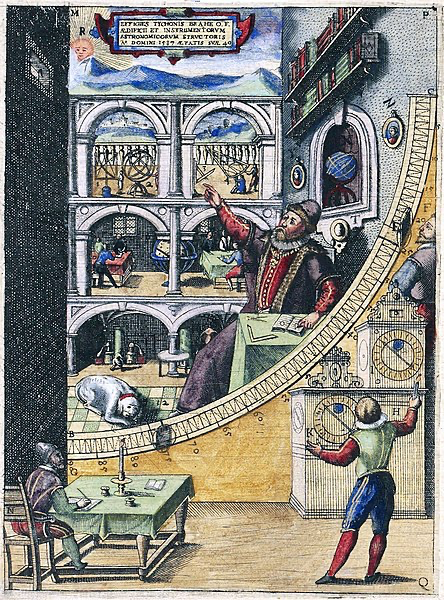
\includegraphics[width=0.5\textwidth]{./figures/vertical_tycho_instrumentos.png}
\caption{Este grabado de 1598 muestra el gran cuadrante mural de Tycho
Brahe en \emph{Uraniburgo}, su observatorio astronómico en la isla Hven
en Dinámarca. Con este y otra decena de enormes instrumentos, Tycho
realizó por más de 20 años observaciones de gran precisión de planetas,
estrellas y cometas, que a la larga revolucionarían, no solo la mecánica
celeste, sino también la astronomía en general. Crédito: Royal
Library.\label{fig:tycho_instrumentos}}
\end{figure}

\hypertarget{doscuerpos_sistema_solar}{%
\subsection{Predicciones en el Sistema
Solar}\label{doscuerpos_sistema_solar}}

Podemos usar todo lo visto en este capítulo, para poner a prueba la
afirmación de que es posible predecir con una precisión aceptable para
los estándares astronómicos del pasado (cercana o inferior a 1 minuto de
arco), la posición de los planetas en el Sistema Solar. Para ello
podemos asumir que nuestro sistema planetario, que en realidad esta
formado por decenas de cuerpos de masas no despreciables, puede
describirse como un sistema jerárquico de pares de dos cuerpos:
Sol-Mercurio, Sol-Venus, Sol-Tierra, Sol-Marte, Sol-Asteroide, etc.

Podemos asumir (como lo hicieron implícitamente Kepler y sus
contemporáneos) que la masa del Sol en estos pares de partículas es
infinitamente mayor que la de los cuerpos más pequeño,
\(m_1=m_\odot\approx M\). Con esta aproximación, el Sol se puede asumir
fijo en el centro de masa del sistema (ver Ecs. \ref{eq:r1_r2_r} y
\ref{eq:v1_v2_v}):

\[
\begin{array}{rcl}
\vec r_\odot & \approx & 0\\
\vec v_\odot & \approx & 0\\
\end{array}
\] mientras que el estado de los otros cuerpos es simplemente igual al
vector de estado relativo en el sistema:

\[
\begin{array}{rcl}
\vec r_\mathrm{planeta} & \approx & \vec r\\
\vec v_\mathrm{planeta} & \approx & \vec v
\end{array}
\]

Para poner a prueba la aproximación calcularemos a continuación los
vectores de estado de la Tierra y Marte y deduciremos a partir de ellos
la posición en el cielo del último planeta que después compararemos con
su posición real obtenida con predicciones modernas de alta precisión.

Comencemos entonce por determinar el vector de estado de la Tierra y
Marte respecto al Sol en una fecha específica. Para ello podemos
valernos de la rutina \texttt{spkezr} que introdujimos en el
\autoref{problema_ncuerpos}.

    \begin{code}{}{}\begin{Verbatim}[fontsize=\small,commandchars=\\\{\}]
\PY{k+kn}{from} \PY{n+nn}{spiceypy} \PY{k}{import} \PY{n}{furnsh}
\PY{n}{furnsh}\PY{p}{(}\PY{l+s+s2}{\PYZdq{}}\PY{l+s+s2}{pymcel/data/de430.tpc}\PY{l+s+s2}{\PYZdq{}}\PY{p}{)}
\PY{n}{furnsh}\PY{p}{(}\PY{l+s+s2}{\PYZdq{}}\PY{l+s+s2}{pymcel/data/de430.bsp}\PY{l+s+s2}{\PYZdq{}}\PY{p}{)}

\PY{c+c1}{\PYZsh{}Fecha de referencia J2000.0}
\PY{n}{t0}\PY{o}{=}\PY{l+m+mi}{0}

\PY{c+c1}{\PYZsh{}Parametro gravitacional del sistema}
\PY{k+kn}{from} \PY{n+nn}{spiceypy} \PY{k}{import} \PY{n}{bodvrd}
\PY{n}{mu}\PY{o}{=}\PY{n}{bodvrd}\PY{p}{(}\PY{l+s+s2}{\PYZdq{}}\PY{l+s+s2}{SUN}\PY{l+s+s2}{\PYZdq{}}\PY{p}{,}\PY{l+s+s2}{\PYZdq{}}\PY{l+s+s2}{GM}\PY{l+s+s2}{\PYZdq{}}\PY{p}{,}\PY{l+m+mi}{1}\PY{p}{)}\PY{p}{[}\PY{l+m+mi}{1}\PY{p}{]}\PY{p}{[}\PY{l+m+mi}{0}\PY{p}{]}

\PY{c+c1}{\PYZsh{}Vectores de estado de la Tierra y Marte}
\PY{k+kn}{from} \PY{n+nn}{spiceypy} \PY{k}{import} \PY{n}{spkezr}
\PY{n}{tierra}\PY{p}{,}\PY{n}{tluz}\PY{o}{=}\PY{n}{spkezr}\PY{p}{(}\PY{l+s+s2}{\PYZdq{}}\PY{l+s+s2}{EARTH\PYZus{}BARYCENTER}\PY{l+s+s2}{\PYZdq{}}\PY{p}{,}\PY{n}{t0}\PY{p}{,}\PY{l+s+s2}{\PYZdq{}}\PY{l+s+s2}{ECLIPJ2000}\PY{l+s+s2}{\PYZdq{}}\PY{p}{,}\PY{l+s+s2}{\PYZdq{}}\PY{l+s+s2}{None}\PY{l+s+s2}{\PYZdq{}}\PY{p}{,}\PY{l+s+s2}{\PYZdq{}}\PY{l+s+s2}{SUN}\PY{l+s+s2}{\PYZdq{}}\PY{p}{)}
\PY{n}{rtierra0}\PY{o}{=}\PY{n}{tierra}\PY{p}{[}\PY{p}{:}\PY{l+m+mi}{3}\PY{p}{]}
\PY{n}{vtierra0}\PY{o}{=}\PY{n}{tierra}\PY{p}{[}\PY{l+m+mi}{3}\PY{p}{:}\PY{p}{]}
\PY{n}{marte}\PY{p}{,}\PY{n}{tluz}\PY{o}{=}\PY{n}{spkezr}\PY{p}{(}\PY{l+s+s2}{\PYZdq{}}\PY{l+s+s2}{MARS\PYZus{}BARYCENTER}\PY{l+s+s2}{\PYZdq{}}\PY{p}{,}\PY{n}{t0}\PY{p}{,}\PY{l+s+s2}{\PYZdq{}}\PY{l+s+s2}{ECLIPJ2000}\PY{l+s+s2}{\PYZdq{}}\PY{p}{,}\PY{l+s+s2}{\PYZdq{}}\PY{l+s+s2}{None}\PY{l+s+s2}{\PYZdq{}}\PY{p}{,}\PY{l+s+s2}{\PYZdq{}}\PY{l+s+s2}{SUN}\PY{l+s+s2}{\PYZdq{}}\PY{p}{)}
\PY{n}{rmarte0}\PY{o}{=}\PY{n}{marte}\PY{p}{[}\PY{p}{:}\PY{l+m+mi}{3}\PY{p}{]}
\PY{n}{vmarte0}\PY{o}{=}\PY{n}{marte}\PY{p}{[}\PY{l+m+mi}{3}\PY{p}{:}\PY{p}{]}
\end{Verbatim}

%%

\end{code}
\vspace{-1em}

%%hidecode


    \begin{Verbatim}[fontsize=\small,commandchars=\\\{\}]
Estado inicial de la Tierra (SPICE):
	Posición: [-2.65025770e+07  1.44693956e+08 -1.70505187e+02]
	Velocidad: [-2.97864408e+01 -5.47817684e+00  4.19797701e-05]
Estado inicial de Marte (SPICE):
	Posición: [ 2.08048141e+08 -2.00705251e+06 -5.15628899e+06]
	Velocidad: [ 1.16267242 26.29606454  0.52229699]
\end{Verbatim}

Ahora usaremos la rutina \texttt{propaga\_f\_g} que introdujimos en la
\autoref{funciones_fg} para propagar las posiciones de la Tierra y
Marte, 180 días (aproximadamente 6 meses) en el futuro:

    \begin{code}{Algoritmo}{code:prediccion_ss}\begin{Verbatim}[fontsize=\small,commandchars=\\\{\}]
\PY{c+c1}{\PYZsh{}30 días más tarde}
\PY{n}{t}\PY{o}{=}\PY{l+m+mi}{180}\PY{o}{*}\PY{l+m+mi}{86400}

\PY{c+c1}{\PYZsh{}Propaga la posición de la Tierra}
\PY{k+kn}{from} \PY{n+nn}{pymcel}\PY{n+nn}{.}\PY{n+nn}{export} \PY{k}{import} \PY{n}{propaga\PYZus{}f\PYZus{}g}
\PY{n}{prediccion\PYZus{}tierra}\PY{o}{=}\PY{n}{propaga\PYZus{}f\PYZus{}g}\PY{p}{(}\PY{n}{mu}\PY{p}{,}\PY{n}{rtierra0}\PY{p}{,}\PY{n}{vtierra0}\PY{p}{,}\PY{n}{t0}\PY{p}{,}\PY{n}{t}\PY{p}{,}\PY{n}{verbose}\PY{o}{=}\PY{k+kc}{True}\PY{p}{)}
\PY{n}{rtierra}\PY{o}{=}\PY{n}{prediccion\PYZus{}tierra}\PY{p}{[}\PY{l+m+mi}{5}\PY{p}{]}
\PY{n}{vtierra}\PY{o}{=}\PY{n}{prediccion\PYZus{}tierra}\PY{p}{[}\PY{l+m+mi}{6}\PY{p}{]}

\PY{c+c1}{\PYZsh{}Propaga la posición de Marte}
\PY{n}{prediccion\PYZus{}marte}\PY{o}{=}\PY{n}{propaga\PYZus{}f\PYZus{}g}\PY{p}{(}\PY{n}{mu}\PY{p}{,}\PY{n}{rmarte0}\PY{p}{,}\PY{n}{vmarte0}\PY{p}{,}\PY{n}{t0}\PY{p}{,}\PY{n}{t}\PY{p}{,}\PY{n}{verbose}\PY{o}{=}\PY{k+kc}{True}\PY{p}{)}
\PY{n}{rmarte}\PY{o}{=}\PY{n}{prediccion\PYZus{}marte}\PY{p}{[}\PY{l+m+mi}{5}\PY{p}{]}
\PY{n}{vmarte}\PY{o}{=}\PY{n}{prediccion\PYZus{}marte}\PY{p}{[}\PY{l+m+mi}{6}\PY{p}{]}
\end{Verbatim}

%%

\end{code}
\vspace{-1em}

%%hidecode


    \begin{Verbatim}[fontsize=\small,commandchars=\\\{\}]
Estado propagado de la Tierra (aproximación):
	Posición: [ 2.12651481e+07 -1.50593536e+08  1.84746693e+02]
	Velocidad: [ 2.90111873e+01  4.05388504e+00 -3.91059499e-05]
Estado inicial de Marte (aproximación):
	Posición: [-3.75596491e+07  2.34997200e+08  5.84626235e+06]
	Velocidad: [-23.00765883  -1.7690655    0.52851442]
\end{Verbatim}

Podemos comparar las predicciones realizadas con la teoría de dos
cuerpos con aquellas muy precisas calculadas con las integraciones
numéricas implícitas en los datos de \texttt{SPICE}:

    \begin{code}{}{}\begin{Verbatim}[fontsize=\small,commandchars=\\\{\}]
\PY{c+c1}{\PYZsh{}Vectores de estado de la Tierra y Marte}
\PY{n}{tierra}\PY{p}{,}\PY{n}{tluz}\PY{o}{=}\PY{n}{spkezr}\PY{p}{(}\PY{l+s+s2}{\PYZdq{}}\PY{l+s+s2}{EARTH\PYZus{}BARYCENTER}\PY{l+s+s2}{\PYZdq{}}\PY{p}{,}\PY{n}{t}\PY{p}{,}\PY{l+s+s2}{\PYZdq{}}\PY{l+s+s2}{ECLIPJ2000}\PY{l+s+s2}{\PYZdq{}}\PY{p}{,}\PY{l+s+s2}{\PYZdq{}}\PY{l+s+s2}{None}\PY{l+s+s2}{\PYZdq{}}\PY{p}{,}\PY{l+s+s2}{\PYZdq{}}\PY{l+s+s2}{SUN}\PY{l+s+s2}{\PYZdq{}}\PY{p}{)}
\PY{n}{marte}\PY{p}{,}\PY{n}{tluz}\PY{o}{=}\PY{n}{spkezr}\PY{p}{(}\PY{l+s+s2}{\PYZdq{}}\PY{l+s+s2}{MARS\PYZus{}BARYCENTER}\PY{l+s+s2}{\PYZdq{}}\PY{p}{,}\PY{n}{t}\PY{p}{,}\PY{l+s+s2}{\PYZdq{}}\PY{l+s+s2}{ECLIPJ2000}\PY{l+s+s2}{\PYZdq{}}\PY{p}{,}\PY{l+s+s2}{\PYZdq{}}\PY{l+s+s2}{None}\PY{l+s+s2}{\PYZdq{}}\PY{p}{,}\PY{l+s+s2}{\PYZdq{}}\PY{l+s+s2}{SUN}\PY{l+s+s2}{\PYZdq{}}\PY{p}{)}
\end{Verbatim}

%%

\end{code}
\vspace{-1em}

%%hidecode


    \begin{Verbatim}[fontsize=\small,commandchars=\\\{\}]
Estado propagado de la Tierra (SPICE):
	Posición: [ 2.12704637e+07 -1.50594283e+08  2.98450430e+02]
	Velocidad: [ 2.90108118e+01  4.05407503e+00 -2.81172149e-05]
Estado inicial de Marte (SPICE):
	Posición: [-3.75381027e+07  2.35025828e+08  5.84580453e+06]
	Velocidad: [-23.00526594  -1.7643746    0.52849927]
\end{Verbatim}

Las coincidencias en este caso con los resultados obtenidos con la
teoría de los dos cuerpos (Alg. \ref{code:prediccion_ss}) son
sencillamente notables. Pero vayamos más lejos y hagamos la comparación
que nos propusimos hacer desde el principio, es decir, calculemos la
diferencia entre la posición de Marte en el cielo predicha con la teoría
de dos cuerpos y la real (que asumiremos es la que provee
\texttt{SPICE}.)

Para ello nos valdremos de una nueva rutina \texttt{reclat} que permite
convertir un vector posición en sus correspondientes coordenadas de
latitud y longitud referidas al sistema de referencia usado (en este
caso longitud y latitud eclíptica):

    \begin{code}{}{}\begin{Verbatim}[fontsize=\small,commandchars=\\\{\}]
\PY{k+kn}{from} \PY{n+nn}{spiceypy} \PY{k}{import} \PY{n}{reclat}
\PY{c+c1}{\PYZsh{}Distancia a Marte, longitud y latitud eclíptica del planeta}
\PY{n}{dist}\PY{p}{,}\PY{n}{long}\PY{p}{,}\PY{n}{lat}\PY{o}{=}\PY{n}{reclat}\PY{p}{(}\PY{n}{marte}\PY{p}{[}\PY{p}{:}\PY{l+m+mi}{3}\PY{p}{]}\PY{o}{\PYZhy{}}\PY{n}{tierra}\PY{p}{[}\PY{p}{:}\PY{l+m+mi}{3}\PY{p}{]}\PY{p}{)}
\PY{c+c1}{\PYZsh{}Valores usando la teoría aproximada}
\PY{n}{dist\PYZus{}aprox}\PY{p}{,}\PY{n}{long\PYZus{}aprox}\PY{p}{,}\PY{n}{lat\PYZus{}aprox}\PY{o}{=}\PY{n}{reclat}\PY{p}{(}\PY{n}{rmarte}\PY{o}{\PYZhy{}}\PY{n}{rtierra}\PY{p}{)}
\end{Verbatim}

%%

\end{code}
\vspace{-1em}

%%hidecode


    \begin{Verbatim}[fontsize=\small,commandchars=\\\{\}]
Distancia:
	Real: 390122400.20565176 km
	Aprox.: 390095819.98641676 km
Longitud eclíptica:
	Real: 98.6710192 grados
	Aprox.: 98.6740266 grados
	Diferencia: 0.1804482 arcmin
Latitud eclíptica:
	Real: 0.8585392 grados
	Aprox.: 0.8586816 grados
	Diferencia: 0.0085473 arcmin
\end{Verbatim}

Como lo observo Kepler, el error en la posición en el cielo se mantiene,
por lo menos durante 6 meses por debajo de 1 minuto de arco. En la
\autoref{fig:code:error_posicion_marte}) se muestra el error calculado
en la posición en el cielo, vista desde la Tierra, predicha para el
planeta rojo con la teoría de dos cuerpos.
\vspace{-1em}

%%figcaption::hide::Error en la predicción de la posición de Marte en el cielo, tal y como es visto desde la Tierra, usando la teoría de los dos cuerpos como aproximación al movimiento de ambos planetas.  El error es calculado a lo largo de un período sinódico completo del planeta rojo (780 días.)

%%hidecode


    \begin{center}

\begin{figure}[ht!]
\centering
    \adjustimage{max size={0.8\linewidth}{0.8\paperheight}}{combined_files/combined_1603_0.png}
\caption{Error en la predicción de la posición de Marte en el cielo, tal y como es visto desde la Tierra, usando la teoría de los dos cuerpos como aproximación al movimiento de ambos planetas.  El error es calculado a lo largo de un período sinódico completo del planeta rojo (780 días.).\label{fig:hide}}
\end{figure}

    \end{center}
%{ \hspace*{\fill} \\}
    
\hypertarget{doscuerpos_evolucion_elementos}{%
\subsection{Evolución de los elementos orbitales
osculatrices}\label{doscuerpos_evolucion_elementos}}

Hay un ``fenómeno'' muy interesante que permite entender en parte porque
las predicciones de la teoría de los dos cuerpos usadas aquí para
predecir el estado de las partículas en sistemas jerarquicos de N
cuerpos, no son más precisas. De acuerdo con lo que vimos en la
\autoref{orbita_osculatriz} a cada vector de estado (sea este el
vector de estado de una partícula o el del sistema relativo) podemos
asociar un conjunto de elementos orbitales osculatrices. ¿Cómo son los
elementos osculatrices de las partículas de los sistemas jerarquicos
estudiados en esta sección?

Consideremos por ejemplo el sistema ficticio del principio. Obtengamos
primero la solución numérica a las ecuaciones de movimiento de lo
describen:

    \begin{code}{}{}\begin{Verbatim}[fontsize=\small,commandchars=\\\{\}]
\PY{k+kn}{from} \PY{n+nn}{numpy} \PY{k}{import} \PY{n}{linspace}
\PY{n}{ts}\PY{o}{=}\PY{n}{linspace}\PY{p}{(}\PY{l+m+mf}{0.0}\PY{p}{,}\PY{l+m+mf}{10.0}\PY{p}{,}\PY{l+m+mi}{200}\PY{p}{)}
\PY{k+kn}{from} \PY{n+nn}{pymcel}\PY{n+nn}{.}\PY{n+nn}{export} \PY{k}{import} \PY{n}{ncuerpos\PYZus{}solucion}
\PY{n}{rs}\PY{p}{,}\PY{n}{vs}\PY{p}{,}\PY{n}{rps}\PY{p}{,}\PY{n}{vps}\PY{p}{,}\PY{n}{constantes}\PY{o}{=}\PY{n}{ncuerpos\PYZus{}solucion}\PY{p}{(}\PY{n}{sistema}\PY{p}{,}\PY{n}{ts}\PY{p}{)}
\end{Verbatim}

%%

\end{code}

Para calcular los elementos osculatrices, obtengamos primero la posición
del centro de masa de los sistemas A y B en los que descompusimos el
sistema completo:

    \begin{code}{}{}\begin{Verbatim}[fontsize=\small,commandchars=\\\{\}]
\PY{c+c1}{\PYZsh{}Sistema A}
\PY{n}{r\PYZus{}CM\PYZus{}A}\PY{o}{=}\PY{p}{(}\PY{n}{sistema}\PY{p}{[}\PY{l+m+mi}{0}\PY{p}{]}\PY{p}{[}\PY{l+s+s2}{\PYZdq{}}\PY{l+s+s2}{m}\PY{l+s+s2}{\PYZdq{}}\PY{p}{]}\PY{o}{*}\PY{n}{rs}\PY{p}{[}\PY{l+m+mi}{0}\PY{p}{]}\PY{o}{+}\PY{n}{sistema}\PY{p}{[}\PY{l+m+mi}{1}\PY{p}{]}\PY{p}{[}\PY{l+s+s2}{\PYZdq{}}\PY{l+s+s2}{m}\PY{l+s+s2}{\PYZdq{}}\PY{p}{]}\PY{o}{*}\PY{n}{rs}\PY{p}{[}\PY{l+m+mi}{1}\PY{p}{]}\PY{p}{)}\PY{o}{/}\PY{n}{masaA}
\PY{n}{v\PYZus{}CM\PYZus{}A}\PY{o}{=}\PY{p}{(}\PY{n}{sistema}\PY{p}{[}\PY{l+m+mi}{0}\PY{p}{]}\PY{p}{[}\PY{l+s+s2}{\PYZdq{}}\PY{l+s+s2}{m}\PY{l+s+s2}{\PYZdq{}}\PY{p}{]}\PY{o}{*}\PY{n}{vs}\PY{p}{[}\PY{l+m+mi}{0}\PY{p}{]}\PY{o}{+}\PY{n}{sistema}\PY{p}{[}\PY{l+m+mi}{1}\PY{p}{]}\PY{p}{[}\PY{l+s+s2}{\PYZdq{}}\PY{l+s+s2}{m}\PY{l+s+s2}{\PYZdq{}}\PY{p}{]}\PY{o}{*}\PY{n}{vs}\PY{p}{[}\PY{l+m+mi}{1}\PY{p}{]}\PY{p}{)}\PY{o}{/}\PY{n}{masaA}
\PY{c+c1}{\PYZsh{}Sistema B}
\PY{n}{r\PYZus{}CM\PYZus{}B}\PY{o}{=}\PY{p}{(}\PY{n}{sistemaB}\PY{p}{[}\PY{l+m+mi}{0}\PY{p}{]}\PY{p}{[}\PY{l+s+s2}{\PYZdq{}}\PY{l+s+s2}{m}\PY{l+s+s2}{\PYZdq{}}\PY{p}{]}\PY{o}{*}\PY{n}{r\PYZus{}CM\PYZus{}A}\PY{o}{+}\PY{n}{sistemaB}\PY{p}{[}\PY{l+m+mi}{1}\PY{p}{]}\PY{p}{[}\PY{l+s+s2}{\PYZdq{}}\PY{l+s+s2}{m}\PY{l+s+s2}{\PYZdq{}}\PY{p}{]}\PY{o}{*}\PY{n}{rs}\PY{p}{[}\PY{l+m+mi}{2}\PY{p}{]}\PY{p}{)}\PY{o}{/}\PY{n}{masaB}
\PY{n}{v\PYZus{}CM\PYZus{}B}\PY{o}{=}\PY{p}{(}\PY{n}{sistemaB}\PY{p}{[}\PY{l+m+mi}{0}\PY{p}{]}\PY{p}{[}\PY{l+s+s2}{\PYZdq{}}\PY{l+s+s2}{m}\PY{l+s+s2}{\PYZdq{}}\PY{p}{]}\PY{o}{*}\PY{n}{v\PYZus{}CM\PYZus{}A}\PY{o}{+}\PY{n}{sistemaB}\PY{p}{[}\PY{l+m+mi}{1}\PY{p}{]}\PY{p}{[}\PY{l+s+s2}{\PYZdq{}}\PY{l+s+s2}{m}\PY{l+s+s2}{\PYZdq{}}\PY{p}{]}\PY{o}{*}\PY{n}{vs}\PY{p}{[}\PY{l+m+mi}{2}\PY{p}{]}\PY{p}{)}\PY{o}{/}\PY{n}{masaB}
\end{Verbatim}

%%

\end{code}

Para calcular los elementos osculatrices de la partícula 3, por ejemplo,
debemos primero expresar su vector de estado respecto al centro de masa
de su respectivo subsistema (sistema B) y de allí usar los
procedimientos matemáticos que vimos en la
\autoref{determinacion_orbita} y que se implementan (como vimos en
la \autoref{doscuerpos_spice}) con la rutina \texttt{oscelt}:

    \begin{code}{}{}\begin{Verbatim}[fontsize=\small,commandchars=\\\{\}]
\PY{n}{r3\PYZus{}CM}\PY{o}{=}\PY{n}{rs}\PY{p}{[}\PY{l+m+mi}{2}\PY{p}{]}\PY{o}{\PYZhy{}}\PY{n}{r\PYZus{}CM\PYZus{}B}
\PY{n}{v3\PYZus{}CM}\PY{o}{=}\PY{n}{vs}\PY{p}{[}\PY{l+m+mi}{2}\PY{p}{]}\PY{o}{\PYZhy{}}\PY{n}{v\PYZus{}CM\PYZus{}B}

\PY{n}{Es}\PY{o}{=}\PY{p}{[}\PY{p}{]}
\PY{k}{for} \PY{n}{i}\PY{p}{,}\PY{n}{t} \PY{o+ow}{in} \PY{n+nb}{enumerate}\PY{p}{(}\PY{n}{ts}\PY{p}{)}\PY{p}{:}
    \PY{k+kn}{from} \PY{n+nn}{spiceypy} \PY{k}{import} \PY{n}{oscelt}
    \PY{n}{Es}\PY{o}{+}\PY{o}{=}\PY{p}{[}\PY{n}{oscelt}\PY{p}{(}\PY{n+nb}{list}\PY{p}{(}\PY{n}{r3\PYZus{}CM}\PY{p}{[}\PY{n}{i}\PY{p}{]}\PY{p}{)}\PY{o}{+}\PY{n+nb}{list}\PY{p}{(}\PY{n}{v3\PYZus{}CM}\PY{p}{[}\PY{n}{i}\PY{p}{]}\PY{p}{)}\PY{p}{,}\PY{n}{t}\PY{p}{,}\PY{n}{masaB}\PY{p}{)}\PY{p}{]}

\PY{k+kn}{from} \PY{n+nn}{numpy} \PY{k}{import} \PY{n}{array}
\PY{n}{Es}\PY{o}{=}\PY{n}{array}\PY{p}{(}\PY{n}{Es}\PY{p}{)}
\end{Verbatim}

%%

\end{code}

Podemos ahora graficar los elementos orbitales \(q\), \(e\), \(i\),
\(\Omega\), \(\omega\) como función del tiempo:

    \begin{code}{Algoritmo}{code:variacion_elementos}\begin{Verbatim}[fontsize=\small,commandchars=\\\{\}]
\PY{k+kn}{import} \PY{n+nn}{matplotlib}\PY{n+nn}{.}\PY{n+nn}{pyplot} \PY{k}{as} \PY{n+nn}{plt}
\PY{n}{fig}\PY{p}{,}\PY{n}{axs}\PY{o}{=}\PY{n}{plt}\PY{o}{.}\PY{n}{subplots}\PY{p}{(}\PY{l+m+mi}{5}\PY{p}{,}\PY{l+m+mi}{1}\PY{p}{,}\PY{n}{figsize}\PY{o}{=}\PY{p}{(}\PY{l+m+mi}{5}\PY{p}{,}\PY{l+m+mi}{8}\PY{p}{)}\PY{p}{,}\PY{n}{sharex}\PY{o}{=}\PY{k+kc}{True}\PY{p}{)}

\PY{c+c1}{\PYZsh{}Periapsis}
\PY{n}{axs}\PY{p}{[}\PY{l+m+mi}{0}\PY{p}{]}\PY{o}{.}\PY{n}{plot}\PY{p}{(}\PY{n}{ts}\PY{p}{,}\PY{n}{Es}\PY{p}{[}\PY{p}{:}\PY{p}{,}\PY{l+m+mi}{0}\PY{p}{]}\PY{p}{)}
\PY{n}{axs}\PY{p}{[}\PY{l+m+mi}{0}\PY{p}{]}\PY{o}{.}\PY{n}{set\PYZus{}ylabel}\PY{p}{(}\PY{l+s+s2}{\PYZdq{}}\PY{l+s+s2}{\PYZdl{}q\PYZdl{} (u.c.)}\PY{l+s+s2}{\PYZdq{}}\PY{p}{)}
\PY{c+c1}{\PYZsh{}Excentricidad}
\PY{n}{axs}\PY{p}{[}\PY{l+m+mi}{1}\PY{p}{]}\PY{o}{.}\PY{n}{plot}\PY{p}{(}\PY{n}{ts}\PY{p}{,}\PY{n}{Es}\PY{p}{[}\PY{p}{:}\PY{p}{,}\PY{l+m+mi}{1}\PY{p}{]}\PY{p}{)}
\PY{n}{axs}\PY{p}{[}\PY{l+m+mi}{1}\PY{p}{]}\PY{o}{.}\PY{n}{set\PYZus{}ylabel}\PY{p}{(}\PY{l+s+s2}{\PYZdq{}}\PY{l+s+s2}{\PYZdl{}e\PYZdl{} (u.c.)}\PY{l+s+s2}{\PYZdq{}}\PY{p}{)}
\PY{c+c1}{\PYZsh{}Inclinación}
\PY{n}{axs}\PY{p}{[}\PY{l+m+mi}{2}\PY{p}{]}\PY{o}{.}\PY{n}{plot}\PY{p}{(}\PY{n}{ts}\PY{p}{,}\PY{n}{Es}\PY{p}{[}\PY{p}{:}\PY{p}{,}\PY{l+m+mi}{2}\PY{p}{]}\PY{o}{*}\PY{l+m+mi}{180}\PY{o}{/}\PY{n}{pi}\PY{p}{)}
\PY{n}{axs}\PY{p}{[}\PY{l+m+mi}{2}\PY{p}{]}\PY{o}{.}\PY{n}{set\PYZus{}ylabel}\PY{p}{(}\PY{l+s+s2}{\PYZdq{}}\PY{l+s+s2}{\PYZdl{}i\PYZdl{} (grados)}\PY{l+s+s2}{\PYZdq{}}\PY{p}{)}
\PY{c+c1}{\PYZsh{}Longitud del nodo ascendente}
\PY{n}{axs}\PY{p}{[}\PY{l+m+mi}{3}\PY{p}{]}\PY{o}{.}\PY{n}{plot}\PY{p}{(}\PY{n}{ts}\PY{p}{,}\PY{n}{Es}\PY{p}{[}\PY{p}{:}\PY{p}{,}\PY{l+m+mi}{3}\PY{p}{]}\PY{o}{*}\PY{l+m+mi}{180}\PY{o}{/}\PY{n}{pi}\PY{p}{)}
\PY{n}{axs}\PY{p}{[}\PY{l+m+mi}{3}\PY{p}{]}\PY{o}{.}\PY{n}{set\PYZus{}ylabel}\PY{p}{(}\PY{l+s+s2}{\PYZdq{}}\PY{l+s+s2}{\PYZdl{}}\PY{l+s+s2}{\PYZbs{}}\PY{l+s+s2}{Omega\PYZdl{} (grados)}\PY{l+s+s2}{\PYZdq{}}\PY{p}{)}
\PY{c+c1}{\PYZsh{}Argumento del periapsis}
\PY{n}{cond}\PY{o}{=}\PY{n}{Es}\PY{p}{[}\PY{p}{:}\PY{p}{,}\PY{l+m+mi}{4}\PY{p}{]}\PY{o}{\PYZgt{}}\PY{n}{pi}
\PY{n}{Es}\PY{p}{[}\PY{n}{cond}\PY{p}{,}\PY{l+m+mi}{4}\PY{p}{]}\PY{o}{=}\PY{n}{Es}\PY{p}{[}\PY{n}{cond}\PY{p}{,}\PY{l+m+mi}{4}\PY{p}{]}\PY{o}{\PYZhy{}}\PY{l+m+mi}{2}\PY{o}{*}\PY{n}{pi}
\PY{n}{axs}\PY{p}{[}\PY{l+m+mi}{4}\PY{p}{]}\PY{o}{.}\PY{n}{plot}\PY{p}{(}\PY{n}{ts}\PY{p}{,}\PY{n}{Es}\PY{p}{[}\PY{p}{:}\PY{p}{,}\PY{l+m+mi}{4}\PY{p}{]}\PY{o}{*}\PY{l+m+mi}{180}\PY{o}{/}\PY{n}{pi}\PY{p}{)}
\PY{n}{axs}\PY{p}{[}\PY{l+m+mi}{4}\PY{p}{]}\PY{o}{.}\PY{n}{set\PYZus{}ylabel}\PY{p}{(}\PY{l+s+s2}{\PYZdq{}}\PY{l+s+s2}{\PYZdl{}}\PY{l+s+s2}{\PYZbs{}}\PY{l+s+s2}{omega\PYZdl{} (grados)}\PY{l+s+s2}{\PYZdq{}}\PY{p}{)}

\PY{c+c1}{\PYZsh{}Decoración}
\PY{n}{axs}\PY{p}{[}\PY{o}{\PYZhy{}}\PY{l+m+mi}{1}\PY{p}{]}\PY{o}{.}\PY{n}{set\PYZus{}xlabel}\PY{p}{(}\PY{l+s+s2}{\PYZdq{}}\PY{l+s+s2}{\PYZdl{}t\PYZdl{} (u.c.)}\PY{l+s+s2}{\PYZdq{}}\PY{p}{)}
\PY{n}{fig}\PY{o}{.}\PY{n}{tight\PYZus{}layout}\PY{p}{(}\PY{p}{)}
\end{Verbatim}

%%

\tcblower
\footnotesize
\em ver Figura \ref{fig:code:variacion_elementos}
\end{code}

    \begin{center}

\begin{figure}[ht!]
\centering
    \adjustimage{max size={0.8\linewidth}{0.8\paperheight}}{combined_files/combined_1613_0.png}
\caption{Figura correspondiente al código \ref{code:variacion_elementos}.\label{fig:code:variacion_elementos}}
\end{figure}

    \end{center}
%{ \hspace*{\fill} \\}
    
Como vemos en la \autoref{fig:code:variacion_elementos} el valor de los
elementos orbitales osculatrices de la partícula 3 no es constante por
lo que no es de extrañar que las predicciones que hicimos de la posición
de esa partícula con la teoría de los dos cuerpos, y que esencialmente
asumen que la órbita tiene elementos constantes e iguales a aquellos en
\(t=t_0\), no sean muy precisos.

Pero existe un elemento aún más interesante: las variaciones de los
elementos no parecen ser ``arbitrarias'' o ``aleatorias. En el caso de
\(q\), \(e\), \(i\) y \(\omega\) los elementos''oscilan" de formas
aparenetemente predecibles alrededor de un valor promedio, con
amplitudes muy pequeñas y frecuencias similares. Por su parte, el valor
de \(\Omega\) parece aumentar monótonamente, con algunos cambios en la
tasa de variación que ocurren también a intervalos regulares de tiempo.

\hypertarget{elementos_luna}{%
\subsection{Un ejemplo real: los elementos osculatrices de la
Luna}\label{elementos_luna}}

El curioso comportamiento observado en el sistema ficticio estudiado en
esta sección, es también observado en sistemas astronómicos reales. El
caso más notable en el Sistema Solar es el de la Luna. En el algoritmo a
continuación calculamos los elementos osculatrices de nuestro satélites,
relativos al centro de masa del sistema Tierra-Luna, durante un año
completo.

    \begin{code}{}{}\begin{Verbatim}[fontsize=\small,commandchars=\\\{\}]
\PY{c+c1}{\PYZsh{}Masa del sistema}
\PY{k+kn}{from} \PY{n+nn}{spiceypy} \PY{k}{import} \PY{n}{bodvrd}
\PY{n}{mu}\PY{o}{=}\PY{n}{bodvrd}\PY{p}{(}\PY{l+s+s2}{\PYZdq{}}\PY{l+s+s2}{EARTH}\PY{l+s+s2}{\PYZdq{}}\PY{p}{,}\PY{l+s+s2}{\PYZdq{}}\PY{l+s+s2}{GM}\PY{l+s+s2}{\PYZdq{}}\PY{p}{,}\PY{l+m+mi}{1}\PY{p}{)}\PY{p}{[}\PY{l+m+mi}{1}\PY{p}{]}\PY{p}{[}\PY{l+m+mi}{0}\PY{p}{]}\PY{o}{+}\PY{n}{bodvrd}\PY{p}{(}\PY{l+s+s2}{\PYZdq{}}\PY{l+s+s2}{MOON}\PY{l+s+s2}{\PYZdq{}}\PY{p}{,}\PY{l+s+s2}{\PYZdq{}}\PY{l+s+s2}{GM}\PY{l+s+s2}{\PYZdq{}}\PY{p}{,}\PY{l+m+mi}{1}\PY{p}{)}\PY{p}{[}\PY{l+m+mi}{1}\PY{p}{]}\PY{p}{[}\PY{l+m+mi}{0}\PY{p}{]}

\PY{k+kn}{from} \PY{n+nn}{numpy} \PY{k}{import} \PY{n}{linspace}
\PY{n}{ts}\PY{o}{=}\PY{n}{linspace}\PY{p}{(}\PY{l+m+mi}{0}\PY{p}{,}\PY{l+m+mi}{180}\PY{o}{*}\PY{l+m+mi}{86400}\PY{p}{,}\PY{l+m+mi}{100}\PY{p}{)}
\PY{n}{Es}\PY{o}{=}\PY{p}{[}\PY{p}{]}
\PY{k}{for} \PY{n}{t} \PY{o+ow}{in} \PY{n}{ts}\PY{p}{:}
    \PY{c+c1}{\PYZsh{}Vector de estado de la Luna}
    \PY{k+kn}{from} \PY{n+nn}{spiceypy} \PY{k}{import} \PY{n}{spkezr}
    \PY{n}{luna}\PY{p}{,}\PY{n}{tluz}\PY{o}{=}\PY{n}{spkezr}\PY{p}{(}\PY{l+s+s2}{\PYZdq{}}\PY{l+s+s2}{MOON}\PY{l+s+s2}{\PYZdq{}}\PY{p}{,}\PY{n}{t}\PY{p}{,}\PY{l+s+s2}{\PYZdq{}}\PY{l+s+s2}{J2000}\PY{l+s+s2}{\PYZdq{}}\PY{p}{,}\PY{l+s+s2}{\PYZdq{}}\PY{l+s+s2}{None}\PY{l+s+s2}{\PYZdq{}}\PY{p}{,}\PY{l+s+s2}{\PYZdq{}}\PY{l+s+s2}{EARTH\PYZus{}BARYCENTER}\PY{l+s+s2}{\PYZdq{}}\PY{p}{)}
    
    \PY{c+c1}{\PYZsh{}Elementos osculatrices}
    \PY{k+kn}{from} \PY{n+nn}{spiceypy} \PY{k}{import} \PY{n}{oscelt}
    \PY{n}{Es}\PY{o}{+}\PY{o}{=}\PY{p}{[}\PY{n}{oscelt}\PY{p}{(}\PY{n}{luna}\PY{p}{,}\PY{n}{t}\PY{p}{,}\PY{n}{mu}\PY{p}{)}\PY{p}{]}

\PY{k+kn}{from} \PY{n+nn}{numpy} \PY{k}{import} \PY{n}{array}
\PY{n}{Es}\PY{o}{=}\PY{n}{array}\PY{p}{(}\PY{n}{Es}\PY{p}{)}
\end{Verbatim}

%%

\end{code}

Una gráfica de los elementos osculatirces calculados aquí como función
del tiempo (medido en \emph{periodos sinódicos}, es decir el tiempo de
Luna llena a Luna llena) se muestra en la
\autoref{fig:code:variacion_elementos}. Como vemos allí y como
observamos también en el sistema ficticio, existen variaciones
periódicas en los elementos orbitales de la Luna. Adicionalmente, el
período de variación de la excentricidad y la distancia al periapsis de
la Luna es exactamente igual al período sinódico: la excentricidad, por
ejemplo siempre es mínima cuando la Luna esta cerca a la luna nueva.
\vspace{-1em}

%%figcaption::hide::Variaciones de los elementos orbitales osculatrices de la Luna respecto al baricentro del sistema Tierra-Luna.  

%%hidecode


    \begin{center}

\begin{figure}[ht!]
\centering
    \adjustimage{max size={0.8\linewidth}{0.8\paperheight}}{combined_files/combined_1620_0.png}
\caption{Variaciones de los elementos orbitales osculatrices de la Luna respecto al baricentro del sistema Tierra-Luna.  .\label{fig:hide}}
\end{figure}

    \end{center}
%{ \hspace*{\fill} \\}
    
\bigskip

¿De qué dependen estas variaciones en los elementos osculatrices? ¿cómo
puede predecirse y de qué manera su predicción puede ayudarnos a
describir sistemas jerárquicos de N cuerpos? La solución a este problema
obsesionó a Newton hasta el final de su vida y fue necesario una nueva
generación de matemáticos en los 1700, entre ellos Joseph Louis
Lagrange, para resolver satisfactoriamente el problema. En la siguiente
sección abordaremos algunas nociones básicas del problema. Un desarrollo
a fondo del mismo es parte de textos más avanzados de Mecánica Celeste.



\hypertarget{teoria_perturbaciones}{%
\section{Introducción a la teoría de
perturbaciones}\label{teoria_perturbaciones}}

En la \autoref{doscuerpos_epsilon} vimos que en el problema de los
dos cuerpos la siguiente cantidad es constante:

\[
\frac{v^2}{2}-\frac{\mu}{r}=\epsilon
\]

Por otra parte usando la \emph{vis viva} (Ec. \ref{eq:vis_viva})
encontramos que en el caso de órbitas no parábolicas, \(e\neq 1\), el
valor de la constante \(\epsilon\) puede expresarse en términos del
semieje mayor \(a\) de la órbita como:

\[
\epsilon=-\frac{\mu}{2a}
\]

En la última sección vimos sin embargo que en sistemas jerarquicos de N
cuerpos, en los que se describe la dinámica como la superposición de N-1
subsistemas dos cuerpos, el valor los elementos orbitales de los
subsistemas, incluyendo el semiejemayor \(a\) puede cambiar en el
tiempo. Si admitimos esto. el valor de \(\epsilon\) en esos sistemas
puede cambiar y lo hará a una tasa que puede expresarse como:

\begin{equation}
\label{eq:dot_epsilon_preliminar}
\dot{\epsilon}=\frac{\mu}{2a^2}\dot{a}
\end{equation}

Esta ecuación esconde el secreto de la pregunta que nos hacíamos al
final de la sección anterior: para calcular la variación de \(a\) (y tal
vez de otros elementos orbitales) es necesario calcular la variación de
\(\epsilon\) \cite{Burns1976Perturbations}.

\hypertarget{perturbacion_a}{%
\subsection{Perturbación del semieje mayor}\label{perturbacion_a}}

Por el teorema de conservación de la energía (Teo.
\ref{box:teo:conservacion.energia}) la tasa de variación en la energía
mecánica de una partícula que esta sometida a una fuerza no conservativa
\(\vec F\) es:

\[
\dot{E}=\dot{\vec r}\cdot \vec F
\]

Supongamos que el sistema de dos cuerpos esta sometido a una fuerza
(específica) neta externa \(\Delta\vec f\ll -\mu{\vec r}/r^3\), que
podemos escribir en términos de los vectores unitarios de coordenadas
cilíndricas como:

\[
\Delta\vec f=R{\hat e}_r+T{\hat e}_v+N{\hat e}_h
\]

Llamamo a \(\Delta\vec f\) la \textbf{fuerza perturbadora}.

\begin{figure}[t!]
\centering
\includegraphics[width=0.8\textwidth]{./figures/square_fuerza_perturbadora.png}
\caption{Fuerza perturbadora neta \(\Delta\vec f\) actuando sobre el
vector relativo en el problema de los dos
cuerpos.\label{fig:fuerza_perturbadora}}
\end{figure}

En términos de esta fuerza y del teorema de conservación de la energía,
la variación en la energía específica se puede escribir como:

\[
\dot \epsilon=R\dot r + Tr{\dot f}
\]

De otra parte, derivando la ecuación de la trayectoria (Ec.
\label{eq:doscuerpos_trayectoria}):

\[
\dot r=\frac{pe{\dot f}\sin f}{1+e\cos f}
\] y usando el hecho de que sobre una cónica \(r^2\dot f=\sqrt{\mu p}\),
la variación de la energía relativa específica se puede escribir como:

\begin{equation}
\label{eq:dot_epsilon}
\dot \epsilon=\sqrt{\frac{\mu}{p}}\left[eR\sin f+T(1+e\cos f)\right]
\end{equation}

Reemplazando en la Ec. (\ref{eq:dot_epsilon_preliminar}) y despejando
\(\dot a\) obtenemos finalmente:

\begin{equation}
\label{eq:dot_a}
\dot a=2\sqrt{\frac{a^3}{\mu(1-e^2)}}\left[eR\sin f+T(1+e\cos f)\right]
\end{equation}

Como vemos solo las componentes radial y tangencial de la fuerza
perturbadora pueden efectivamente cambiar el tamaño de la órbita. Las
perturbaciones perpendiculaes al plano orbital no tienen un efecto sobre
el tamaño, aunque sí sobre su orientación como veremos más adelante.

\hypertarget{perturbacion_e}{%
\subsection{Perturbación de la excéntricidad}\label{perturbacion_e}}

Si la energía relativa específica se altera por la acción de una fuerza
perturbadora, la excentricidad de la órbita también será perturbada en
virtud de la relación que ambas cantidades guardan de acuerdo con la Ec.
(\ref{eq:e_h_epsilon}):

\[
e=\sqrt{1+\frac{2\epsilon h^2}{\mu^2}}
\]

La tasa de cambio de \(e\) será:

\[
\dot e=\frac{1}{2e}\left(2\frac{h^2{\dot\epsilon}}{\mu^2}+4\frac{\epsilon h{\dot h}}{\mu^2}\right)
\]

Teniendo en cuenta que de acuerdo a la Ec. (\ref{eq:e_h_epsilon}):

\[
\frac{2\epsilon h^2}{\mu^2}=e^2-1
\] la variación en la excentricidad se puede escribir como:

\begin{equation}
\label{eq:dot_e_preliminar}
\dot e=\frac{e^2-1}{2e}\left(\frac{\dot\epsilon}{\epsilon}+2\frac{\dot h}{h}\right)
\end{equation}

La tasa de variación del momento angular específico se puede calcular
con la ayuda de la torca (ver \autoref{cantidades_dinamicas}):

\[
\dot{\vec h}=\vec r\times \Delta \vec f=rT\hat{e}_h-rN\hat{e}_v
\]

Por otro lado si escribimos \(\vec h=h\hat{e}_h\), y admitimos que la
fuerza perturbadora puede cambiar la inclinación y orientación del
plano, es decir \(\dot{\hat{e}}_h\neq \vec o\):

\[
\dot{\vec h}={\dot h}{\hat e}_h+h\dot{\hat e}_h
\]

La comparación de estas dos últimas ecuaciones permite escribir:

\[
\dot h=rT
\]

Reemplazando esta expresión y la Ec. (\ref{eq:dot_epsilon}) en la Ec.
(\ref{eq:dot_e_preliminar}) obtenemos finalmente:

\begin{equation}
\label{eq:dot_e}
\dot e=2\sqrt{\frac{a(1-e^2)}{\mu}}\left[eR\sin f+T(\cos f+\cos E)\right]
\end{equation} donde además hemos usado el hecho que \(r=a(1-e\cos E)\).

Como sucedió con el tamaño, la forma de la órbita, parametrizada por la
excentricidad \(e\) no depende de la componente normal de la fuerza
perturbadora.

\hypertarget{perturbacion_orientacion}{%
\subsection{Perturbaciones de la
orientación}\label{perturbacion_orientacion}}

De manera análoga a como fueron deducidas en las secciones anteriores
las tasas de cambio en el tamaño \(a\) y la forma \(e\) de la órbita
osculatriz, es posible obtener ecuaciones para las tasas de cambio de
los parámetros orbitales que describen su orientación en el espacio,
\(i\), \(\Omega\) y \(\omega\).

En aras de la brevedad y siendo esta sección apenas una introducción a
la teoría de perturbaciones, reproducimos abajo las ecuaciones
correspondientes. Una deducción detallada (y no muy difícil realmente)
puede encontrarse en el artículo clásico de Burns
\cite{Burns1976Perturbations} o en el reconocido texto de Murray y
Dermott \cite{Murray1999}.

La tasa de cambio de los parámetros de orientación de la órbita está
dada por:

\begin{eqnarray}
\label{eq:dot_i}
\dot i & = & \sqrt{\frac{a(1-e^2)}{\mu}}\frac{\cos(\omega+f)}{1+e\cos f}N \\
\label{eq:dot_Omega}
\dot \Omega & = & \sqrt{\frac{a(1-e^2)}{\mu}}\frac{\sin(\omega+f)}{\sin i(1+e\cos f)}N\\
\label{eq:dot_omega}
\dot \omega & = & \frac{1}{e}\sqrt{\frac{a(1-e^2)}{\mu}}\left[-R\cos f+T\sin f\frac{2+e\cos f}{1+e\cos f}\right]-\dot\Omega\cos i
\end{eqnarray}

\hypertarget{ecuaciuxf3n-de-la-uxf3rbita-osculatriz}{%
\subsection{Ecuación de la órbita
osculatriz}\label{ecuaciuxf3n-de-la-uxf3rbita-osculatriz}}

En todas las ecuaciones anteriores aparecen explícitas las componentes
de la fuerza perturbadora \(\Delta\vec f\). Pero ¿dónde aparece en estas
ecuaciones la fuerza central de magnitud \(\mu/r^2\) que domina el
movimiento relativo del sistema? El efecto de esta fuerza se ha hecho
implícito al asumir, de un lado, que la ecuación de la trayectoria es:

\[
r=\frac{a(1-e^2)}{1+e\cos f}
\] y que instantáneamente se satisface la relación:

\[
h=r^2\dot f
\]

Ambas ecuaciones son justamente el resultado de la integración de las
ecuaciones de movimiento del problema relativo.

Despejando \(\dot f\) en la última ecuación y usando la ecuación de la
trayectoria escrita antes, podemos finalmente escribir la ecuación:

\begin{equation}
\label{eq:dot_f}
\dot f=\sqrt{\frac{\mu}{a^3(1-e^2)^3}}\;(1+e\cos f)^2
\end{equation}

\bigskip

En síntesis, las ecuaciones (\ref{eq:dot_a}), (\ref{eq:dot_e}),
(\ref{eq:dot_i}), (\ref{eq:dot_Omega}), (\ref{eq:dot_omega}) y
(\ref{eq:dot_f}), ofrecen una descripción completa del movimiento en el
tiempo de un cuerpo sometido a una fuerza central con parámetro
gravitacional \(\mu\) y perturbado por una pequeña fuerza
\(\Delta\vec f=T\hat{e}_r+R\hat{e}_v+N\hat{e}_h\).

Estas ecuaciones constituyen un problema de valor inicial (IVP) en el
que dados un conjunto de elementos orbitales iniciales
\((a_0,e_0,i_0,\Omega_0,\omega_0,f_0)\) y una vez especificada la manera
como las componentes de la fuerza perturbadora depende del estado del
sistema, es posible calcular los elementos orbitales y de allí el estado
del sistema en cualquier instante del tiempo futuro.

La implicaciones teóricas de estas ecuaciones están más allá del nivel
de este libro y se desarrollan como parte de la teoría general de
perturbaciones. En la siguiente sección ilustraremos, con la ayuda de
las herramientas algoritmicas vistas en el libro, su aplicación en casos
particulares.

\hypertarget{perturbaciones_ejemplo}{%
\subsection{Un ejemplo numérico}\label{perturbaciones_ejemplo}}

Consideremos por ejemplo el siguiente sistema jerarquico de tres
cuerpos:
%%HIDE%%
    \begin{code}{Algoritmo}{code:ejemplo_sistema_perturbado}\begin{Verbatim}[fontsize=\small,commandchars=\\\{\}]
\PY{k+kn}{from} \PY{n+nn}{numpy} \PY{k}{import} \PY{n}{array}
\PY{n}{sistema}\PY{o}{=}\PY{p}{[}
    \PY{n+nb}{dict}\PY{p}{(}
        \PY{n}{m}\PY{o}{=}\PY{l+m+mf}{1.0}\PY{p}{,}
        \PY{n}{r}\PY{o}{=}\PY{n}{array}\PY{p}{(}\PY{p}{[}\PY{l+m+mi}{0}\PY{p}{,}\PY{l+m+mi}{0}\PY{p}{,}\PY{l+m+mi}{0}\PY{p}{]}\PY{p}{)}\PY{p}{,}
        \PY{n}{v}\PY{o}{=}\PY{n}{array}\PY{p}{(}\PY{p}{[}\PY{l+m+mi}{0}\PY{p}{,}\PY{l+m+mf}{0.0}\PY{p}{,}\PY{l+m+mi}{0}\PY{p}{]}\PY{p}{)}\PY{p}{,}
    \PY{p}{)}\PY{p}{,}
    \PY{n+nb}{dict}\PY{p}{(}
        \PY{n}{m}\PY{o}{=}\PY{l+m+mf}{1e\PYZhy{}8}\PY{p}{,}
        \PY{n}{r}\PY{o}{=}\PY{n}{array}\PY{p}{(}\PY{p}{[}\PY{l+m+mi}{1}\PY{p}{,}\PY{l+m+mi}{1}\PY{p}{,}\PY{l+m+mi}{0}\PY{p}{]}\PY{p}{)}\PY{p}{,}
        \PY{n}{v}\PY{o}{=}\PY{n}{array}\PY{p}{(}\PY{p}{[}\PY{l+m+mf}{0.2}\PY{p}{,}\PY{l+m+mf}{0.8}\PY{p}{,}\PY{l+m+mf}{0.2}\PY{p}{]}\PY{p}{)}\PY{p}{,}
    \PY{p}{)}\PY{p}{,}
    \PY{n+nb}{dict}\PY{p}{(}
        \PY{n}{m}\PY{o}{=}\PY{l+m+mf}{1e\PYZhy{}5}\PY{p}{,}
        \PY{n}{r}\PY{o}{=}\PY{n}{array}\PY{p}{(}\PY{p}{[}\PY{l+m+mi}{2}\PY{p}{,}\PY{l+m+mi}{0}\PY{p}{,}\PY{l+m+mi}{0}\PY{p}{]}\PY{p}{)}\PY{p}{,}
        \PY{n}{v}\PY{o}{=}\PY{n}{array}\PY{p}{(}\PY{p}{[}\PY{l+m+mi}{0}\PY{p}{,}\PY{l+m+mf}{0.8}\PY{p}{,}\PY{l+m+mi}{0}\PY{p}{]}\PY{p}{)}\PY{p}{,}
    \PY{p}{)}\PY{p}{,}    
\PY{p}{]}

\PY{c+c1}{\PYZsh{}Trayectoria numérica}
\PY{k+kn}{from} \PY{n+nn}{numpy} \PY{k}{import} \PY{n}{linspace} 
\PY{n}{t0}\PY{o}{=}\PY{l+m+mf}{0.0}
\PY{n}{T}\PY{o}{=}\PY{l+m+mf}{100.0}\PY{p}{;}\PY{n}{Nt}\PY{o}{=}\PY{l+m+mi}{1000}
\PY{n}{ts}\PY{o}{=}\PY{n}{linspace}\PY{p}{(}\PY{n}{t0}\PY{p}{,}\PY{n}{T}\PY{p}{,}\PY{n}{Nt}\PY{p}{)}

\PY{k+kn}{from} \PY{n+nn}{pymcel}\PY{n+nn}{.}\PY{n+nn}{export} \PY{k}{import} \PY{n}{ncuerpos\PYZus{}solucion}
\PY{n}{rs\PYZus{}num}\PY{p}{,}\PY{n}{vs\PYZus{}num}\PY{p}{,}\PY{n}{rps\PYZus{}num}\PY{p}{,}\PY{n}{vps\PYZus{}num}\PY{p}{,}\PY{n}{constantes}\PY{o}{=}\PY{n}{ncuerpos\PYZus{}solucion}\PY{p}{(}\PY{n}{sistema}\PY{p}{,}\PY{n}{ts}\PY{p}{)}

\PY{c+c1}{\PYZsh{}Grafíco}
\PY{k+kn}{from} \PY{n+nn}{pymcel}\PY{n+nn}{.}\PY{n+nn}{export} \PY{k}{import} \PY{n}{plot\PYZus{}ncuerpos\PYZus{}3d}
\PY{n}{fig}\PY{o}{=}\PY{n}{plot\PYZus{}ncuerpos\PYZus{}3d}\PY{p}{(}\PY{n}{rps\PYZus{}num}\PY{p}{,}\PY{n}{vps\PYZus{}num}\PY{p}{)}
\end{Verbatim}

%%

\tcblower
\footnotesize
\em ver Figura \ref{fig:code:ejemplo_sistema_perturbado}
\end{code}

    \begin{center}

\begin{figure}[ht!]
\centering
    \adjustimage{max size={0.8\linewidth}{0.8\paperheight}}{combined_files/combined_1659_0.png}
\caption{Figura correspondiente al código \ref{code:ejemplo_sistema_perturbado}.\label{fig:code:ejemplo_sistema_perturbado}}
\end{figure}

    \end{center}
%{ \hspace*{\fill} \\}
    
Como vemos en la \autoref{fig:code:ejemplo_sistema_perturbado} el
sistema esta formado por una gran masa central (la partícula 0), rodeada
de dos cuerpos, uno muy ligero (la partícula 1) que se encuentra en una
órbita interior inclinada y otro de masa intermedia (la partícula 2)
cuya órbita coincide aproximadamente con el plano \(x-y\). Nos
proponemos aquí predecir aproximadamente el movimiento de las partículas
del sistema, usando la teoría de los dos cuerpos y la teoría básica de
perturbaciones introducida en esta sección.

Como lo hicimos en secciones anteriores, lo primero que debemos hacer es
identificar los subsistemas en los que puede descomponerse este sistema
jerarquico. En la \autoref{fig:code:ejemplo_sistema_perturbado}
reconocemos que se trata de un \emph{sistema central}, usando las
categoría que introdujimos en la \autoref{doscuerpos_motivacion},
que puede descomponerse en dos subsistemas:

\begin{itemize}
\tightlist
\item
  Un sistema A formado por la partícula 0 (cuerpo central) y la
  partícula 1, la más liviana
\item
  Un sistema B formado por el cuerpo central y la partícula 2.
\end{itemize}

Usando la solución numérica a las ecuaciones de movimiento obtenidas en
el Alg. (\ref{code:ejemplo_sistema_perturbado}), podemos calcular y
visualizar la evolución de los elementos orbitales del sistema A:

    \begin{code}{Algoritmo}{code:ejemplo_sistemaA_perturbado}\begin{Verbatim}[fontsize=\small,commandchars=\\\{\}]
\PY{c+c1}{\PYZsh{}Estado del sistema A}
\PY{n}{muA}\PY{o}{=}\PY{n}{sistema}\PY{p}{[}\PY{l+m+mi}{0}\PY{p}{]}\PY{p}{[}\PY{l+s+s2}{\PYZdq{}}\PY{l+s+s2}{m}\PY{l+s+s2}{\PYZdq{}}\PY{p}{]}\PY{o}{+}\PY{n}{sistema}\PY{p}{[}\PY{l+m+mi}{1}\PY{p}{]}\PY{p}{[}\PY{l+s+s2}{\PYZdq{}}\PY{l+s+s2}{m}\PY{l+s+s2}{\PYZdq{}}\PY{p}{]}
\PY{n}{r\PYZus{}A}\PY{o}{=}\PY{n}{rs\PYZus{}num}\PY{p}{[}\PY{l+m+mi}{0}\PY{p}{,}\PY{p}{:}\PY{p}{]}\PY{o}{\PYZhy{}}\PY{n}{rs\PYZus{}num}\PY{p}{[}\PY{l+m+mi}{1}\PY{p}{,}\PY{p}{:}\PY{p}{]}
\PY{n}{v\PYZus{}A}\PY{o}{=}\PY{n}{vs\PYZus{}num}\PY{p}{[}\PY{l+m+mi}{0}\PY{p}{,}\PY{p}{:}\PY{p}{]}\PY{o}{\PYZhy{}}\PY{n}{vs\PYZus{}num}\PY{p}{[}\PY{l+m+mi}{1}\PY{p}{,}\PY{p}{:}\PY{p}{]}

\PY{c+c1}{\PYZsh{}Calculo de los elementos orbitales}
\PY{n}{EAs}\PY{o}{=}\PY{p}{[}\PY{p}{]}
\PY{k}{for} \PY{n}{i}\PY{p}{,}\PY{n}{t} \PY{o+ow}{in} \PY{n+nb}{enumerate}\PY{p}{(}\PY{n}{ts}\PY{p}{)}\PY{p}{:}
    \PY{k+kn}{from} \PY{n+nn}{spiceypy} \PY{k}{import} \PY{n}{oscelt}
    \PY{n}{EAs}\PY{o}{+}\PY{o}{=}\PY{p}{[}\PY{n}{oscelt}\PY{p}{(}\PY{n+nb}{list}\PY{p}{(}\PY{n}{r\PYZus{}A}\PY{p}{[}\PY{n}{i}\PY{p}{]}\PY{p}{)}\PY{o}{+}\PY{n+nb}{list}\PY{p}{(}\PY{n}{v\PYZus{}A}\PY{p}{[}\PY{n}{i}\PY{p}{]}\PY{p}{)}\PY{p}{,}\PY{n}{t}\PY{p}{,}\PY{n}{muA}\PY{p}{)}\PY{p}{]}
\PY{k+kn}{from} \PY{n+nn}{numpy} \PY{k}{import} \PY{n}{array}
\PY{n}{EAs}\PY{o}{=}\PY{n}{array}\PY{p}{(}\PY{n}{EAs}\PY{p}{)}

\PY{c+c1}{\PYZsh{}Gráfico}
\PY{k+kn}{import} \PY{n+nn}{matplotlib}\PY{n+nn}{.}\PY{n+nn}{pyplot} \PY{k}{as} \PY{n+nn}{plt}
\PY{n}{fig}\PY{p}{,}\PY{n}{axs}\PY{o}{=}\PY{n}{plt}\PY{o}{.}\PY{n}{subplots}\PY{p}{(}\PY{l+m+mi}{5}\PY{p}{,}\PY{l+m+mi}{1}\PY{p}{,}\PY{n}{figsize}\PY{o}{=}\PY{p}{(}\PY{l+m+mi}{5}\PY{p}{,}\PY{l+m+mi}{8}\PY{p}{)}\PY{p}{,}\PY{n}{sharex}\PY{o}{=}\PY{k+kc}{True}\PY{p}{)}
\PY{k+kn}{from} \PY{n+nn}{numpy} \PY{k}{import} \PY{n}{pi}

\PY{c+c1}{\PYZsh{}Periapsis}
\PY{n}{axs}\PY{p}{[}\PY{l+m+mi}{0}\PY{p}{]}\PY{o}{.}\PY{n}{plot}\PY{p}{(}\PY{n}{ts}\PY{p}{,}\PY{n}{EAs}\PY{p}{[}\PY{p}{:}\PY{p}{,}\PY{l+m+mi}{0}\PY{p}{]}\PY{p}{)}
\PY{n}{axs}\PY{p}{[}\PY{l+m+mi}{0}\PY{p}{]}\PY{o}{.}\PY{n}{set\PYZus{}ylabel}\PY{p}{(}\PY{l+s+s2}{\PYZdq{}}\PY{l+s+s2}{\PYZdl{}q\PYZdl{} (u.c.)}\PY{l+s+s2}{\PYZdq{}}\PY{p}{)}
\PY{c+c1}{\PYZsh{}Excentricidad}
\PY{n}{axs}\PY{p}{[}\PY{l+m+mi}{1}\PY{p}{]}\PY{o}{.}\PY{n}{plot}\PY{p}{(}\PY{n}{ts}\PY{p}{,}\PY{n}{EAs}\PY{p}{[}\PY{p}{:}\PY{p}{,}\PY{l+m+mi}{1}\PY{p}{]}\PY{p}{)}
\PY{n}{axs}\PY{p}{[}\PY{l+m+mi}{1}\PY{p}{]}\PY{o}{.}\PY{n}{set\PYZus{}ylabel}\PY{p}{(}\PY{l+s+s2}{\PYZdq{}}\PY{l+s+s2}{\PYZdl{}e\PYZdl{} (u.c.)}\PY{l+s+s2}{\PYZdq{}}\PY{p}{)}
\PY{c+c1}{\PYZsh{}Inclinación}
\PY{n}{axs}\PY{p}{[}\PY{l+m+mi}{2}\PY{p}{]}\PY{o}{.}\PY{n}{plot}\PY{p}{(}\PY{n}{ts}\PY{p}{,}\PY{n}{EAs}\PY{p}{[}\PY{p}{:}\PY{p}{,}\PY{l+m+mi}{2}\PY{p}{]}\PY{o}{*}\PY{l+m+mi}{180}\PY{o}{/}\PY{n}{pi}\PY{p}{)}
\PY{n}{axs}\PY{p}{[}\PY{l+m+mi}{2}\PY{p}{]}\PY{o}{.}\PY{n}{set\PYZus{}ylabel}\PY{p}{(}\PY{l+s+s2}{\PYZdq{}}\PY{l+s+s2}{\PYZdl{}i\PYZdl{} (grados)}\PY{l+s+s2}{\PYZdq{}}\PY{p}{)}
\PY{c+c1}{\PYZsh{}Longitud del nodo ascendente}
\PY{n}{axs}\PY{p}{[}\PY{l+m+mi}{3}\PY{p}{]}\PY{o}{.}\PY{n}{plot}\PY{p}{(}\PY{n}{ts}\PY{p}{[}\PY{p}{:}\PY{p}{]}\PY{p}{,}\PY{n}{EAs}\PY{p}{[}\PY{p}{:}\PY{p}{,}\PY{l+m+mi}{3}\PY{p}{]}\PY{o}{*}\PY{l+m+mi}{180}\PY{o}{/}\PY{n}{pi}\PY{p}{)}
\PY{n}{axs}\PY{p}{[}\PY{l+m+mi}{3}\PY{p}{]}\PY{o}{.}\PY{n}{set\PYZus{}ylabel}\PY{p}{(}\PY{l+s+s2}{\PYZdq{}}\PY{l+s+s2}{\PYZdl{}}\PY{l+s+s2}{\PYZbs{}}\PY{l+s+s2}{Omega\PYZdl{} (grados)}\PY{l+s+s2}{\PYZdq{}}\PY{p}{)}
\PY{c+c1}{\PYZsh{}Argumento del periapsis}
\PY{n}{axs}\PY{p}{[}\PY{l+m+mi}{4}\PY{p}{]}\PY{o}{.}\PY{n}{plot}\PY{p}{(}\PY{n}{ts}\PY{p}{[}\PY{p}{:}\PY{p}{]}\PY{p}{,}\PY{n}{EAs}\PY{p}{[}\PY{p}{:}\PY{p}{,}\PY{l+m+mi}{4}\PY{p}{]}\PY{o}{*}\PY{l+m+mi}{180}\PY{o}{/}\PY{n}{pi}\PY{p}{)}
\PY{n}{axs}\PY{p}{[}\PY{l+m+mi}{4}\PY{p}{]}\PY{o}{.}\PY{n}{set\PYZus{}ylabel}\PY{p}{(}\PY{l+s+s2}{\PYZdq{}}\PY{l+s+s2}{\PYZdl{}}\PY{l+s+s2}{\PYZbs{}}\PY{l+s+s2}{omega\PYZdl{} (grados)}\PY{l+s+s2}{\PYZdq{}}\PY{p}{)}

\PY{c+c1}{\PYZsh{}Decoración}
\PY{n}{axs}\PY{p}{[}\PY{l+m+mi}{0}\PY{p}{]}\PY{o}{.}\PY{n}{set\PYZus{}title}\PY{p}{(}\PY{l+s+s2}{\PYZdq{}}\PY{l+s+s2}{Elementos orbitales partícula 1}\PY{l+s+s2}{\PYZdq{}}\PY{p}{)}
\PY{n}{axs}\PY{p}{[}\PY{o}{\PYZhy{}}\PY{l+m+mi}{1}\PY{p}{]}\PY{o}{.}\PY{n}{set\PYZus{}xlabel}\PY{p}{(}\PY{l+s+s2}{\PYZdq{}}\PY{l+s+s2}{\PYZdl{}t\PYZdl{} (u.c.)}\PY{l+s+s2}{\PYZdq{}}\PY{p}{)}
\PY{n}{fig}\PY{o}{.}\PY{n}{tight\PYZus{}layout}\PY{p}{(}\PY{p}{)}
\end{Verbatim}

%%

\tcblower
\footnotesize
\em ver Figura \ref{fig:code:ejemplo_sistemaA_perturbado}
\end{code}

    \begin{center}

\begin{figure}[ht!]
\centering
    \adjustimage{max size={0.8\linewidth}{0.8\paperheight}}{combined_files/combined_1663_0.png}
\caption{Figura correspondiente al código \ref{code:ejemplo_sistemaA_perturbado}.\label{fig:code:ejemplo_sistemaA_perturbado}}
\end{figure}

    \end{center}
%{ \hspace*{\fill} \\}
    
Como vemos en la \autoref{fig:code:ejemplo_sistemaA_perturbado} el
movimiento de la partícula más ligera no es para nada \emph{Kepleriano}.
Sus elementos orbitales cambian sin una periodicidad reconocible y como
producto de las perturbaciones producidas por la partícula masiva en la
órbita externa.

Por su parte, una gráfica de la posición del sistema B (la partícula 2),
pone en evidencia que su órbita es Kepleriana, al menos durante el
tiempo de integración, y que los efectos perturbadores producidos por la
presencia de la partícula 1 son despreciables:

    \begin{code}{Algoritmo}{code:7_Problema2Cuerpos_24}\begin{Verbatim}[fontsize=\small,commandchars=\\\{\}]
\PY{c+c1}{\PYZsh{}Estado del sistema B}
\PY{n}{muB}\PY{o}{=}\PY{n}{sistema}\PY{p}{[}\PY{l+m+mi}{0}\PY{p}{]}\PY{p}{[}\PY{l+s+s2}{\PYZdq{}}\PY{l+s+s2}{m}\PY{l+s+s2}{\PYZdq{}}\PY{p}{]}\PY{o}{+}\PY{n}{sistema}\PY{p}{[}\PY{l+m+mi}{2}\PY{p}{]}\PY{p}{[}\PY{l+s+s2}{\PYZdq{}}\PY{l+s+s2}{m}\PY{l+s+s2}{\PYZdq{}}\PY{p}{]}
\PY{n}{r\PYZus{}B}\PY{o}{=}\PY{n}{rs\PYZus{}num}\PY{p}{[}\PY{l+m+mi}{0}\PY{p}{,}\PY{p}{:}\PY{p}{]}\PY{o}{\PYZhy{}}\PY{n}{rs\PYZus{}num}\PY{p}{[}\PY{l+m+mi}{2}\PY{p}{,}\PY{p}{:}\PY{p}{]}
\PY{n}{v\PYZus{}B}\PY{o}{=}\PY{n}{vs\PYZus{}num}\PY{p}{[}\PY{l+m+mi}{0}\PY{p}{,}\PY{p}{:}\PY{p}{]}\PY{o}{\PYZhy{}}\PY{n}{vs\PYZus{}num}\PY{p}{[}\PY{l+m+mi}{2}\PY{p}{,}\PY{p}{:}\PY{p}{]}

\PY{c+c1}{\PYZsh{}Gráfico}
\PY{k+kn}{import} \PY{n+nn}{matplotlib}\PY{n+nn}{.}\PY{n+nn}{pyplot} \PY{k}{as} \PY{n+nn}{plt}
\PY{n}{fig}\PY{o}{=}\PY{n}{plt}\PY{o}{.}\PY{n}{figure}\PY{p}{(}\PY{p}{)}\PY{p}{;}
\PY{n}{ax}\PY{o}{=}\PY{n}{fig}\PY{o}{.}\PY{n}{gca}\PY{p}{(}\PY{p}{)}\PY{p}{;}
\PY{n}{ax}\PY{o}{.}\PY{n}{plot}\PY{p}{(}\PY{n}{r\PYZus{}B}\PY{p}{[}\PY{p}{:}\PY{p}{,}\PY{l+m+mi}{0}\PY{p}{]}\PY{p}{,}\PY{n}{r\PYZus{}B}\PY{p}{[}\PY{p}{:}\PY{p}{,}\PY{l+m+mi}{1}\PY{p}{]}\PY{p}{)}\PY{p}{;}

\PY{c+c1}{\PYZsh{}}
\PY{k+kn}{from} \PY{n+nn}{pymcel}\PY{n+nn}{.}\PY{n+nn}{plot} \PY{k}{import} \PY{n}{fija\PYZus{}ejes\PYZus{}proporcionales}
\PY{n}{fija\PYZus{}ejes\PYZus{}proporcionales}\PY{p}{(}\PY{n}{ax}\PY{p}{,}\PY{n}{r\PYZus{}B}\PY{p}{)}\PY{p}{;}
\end{Verbatim}

%%

\tcblower
\footnotesize
\em ver Figura \ref{fig:code:7_Problema2Cuerpos_24}
\end{code}

    \begin{center}

\begin{figure}[ht!]
\centering
    \adjustimage{max size={0.8\linewidth}{0.8\paperheight}}{combined_files/combined_1666_0.png}
\caption{Figura correspondiente al código \ref{code:7_Problema2Cuerpos_24}.\label{fig:code:7_Problema2Cuerpos_24}}
\end{figure}

    \end{center}
%{ \hspace*{\fill} \\}
    
Así pues, la posición de la partícula 2 puede ser predicha con precisión
usando únicamente la solución al problema de los dos cuerpos. Por su
lado, para calcular la posición de la partícula 1 será necesario
resolver el sistemas de ecuaciones diferenciales encontradas en la
sección anterior.

Para hacerlo usando los métodos y herramientas que vimos en la
\autoref{ecuaciones_diferenciales}, es necesario primero escribir el
sistema en la forma reducida (Ec. \ref{eq:ecuaciones_reducidas}) y para
ello, debemos definir la identificación de las variables del sistema con
las variables auxiliares \(\{Y_i\}\). Una posible identificación es
esta:

\[
Y_0=f, Y_1=a, Y_2=e, Y_3=i, Y_4=\Omega, Y_5=\omega
\]

El aspecto más complicado de la implementación de las ecuaciones de
perturbación es el cálculo de las componentes de la fuerza perturbadora.
Para ello es necesario calcular, en cada momento, la posición de la
partícula 2 y con ella la fuerza sobre la partícula 1:

\[
\Delta\vec f=-\frac{\mu_2}{r_{12}^3}{\vec r}_{12}
\]

Las componentes de la fuerza perturbadora se pueden obtener proyectando
el vector \(\Delta\vec f\) sobre los vectores \(\vec r\), \(\vec v\) y
\(\vec h\):

\begin{eqnarray}
\nonumber
R & = & \frac{\Delta{\vec f}\cdot{\vec r}}{r}\\
\nonumber
T & = & \frac{\Delta{\vec f}\cdot{\vec v}}{v}\\
\nonumber
N & = & \frac{\Delta{\vec f}\cdot{\vec h}}{h}\\
\end{eqnarray}

    \begin{code}{}{}\begin{Verbatim}[fontsize=\small,commandchars=\\\{\}]
\PY{k+kn}{from} \PY{n+nn}{scipy}\PY{n+nn}{.}\PY{n+nn}{interpolate} \PY{k}{import} \PY{n}{interp1d}
\PY{n}{x\PYZus{}A\PYZus{}pred}\PY{o}{=}\PY{n}{interp1d}\PY{p}{(}\PY{n}{ts}\PY{p}{,}\PY{n}{r\PYZus{}A}\PY{p}{[}\PY{p}{:}\PY{p}{,}\PY{l+m+mi}{0}\PY{p}{]}\PY{p}{,}\PY{n}{kind}\PY{o}{=}\PY{l+s+s1}{\PYZsq{}}\PY{l+s+s1}{slinear}\PY{l+s+s1}{\PYZsq{}}\PY{p}{)}
\PY{n}{y\PYZus{}A\PYZus{}pred}\PY{o}{=}\PY{n}{interp1d}\PY{p}{(}\PY{n}{ts}\PY{p}{,}\PY{n}{r\PYZus{}A}\PY{p}{[}\PY{p}{:}\PY{p}{,}\PY{l+m+mi}{1}\PY{p}{]}\PY{p}{,}\PY{n}{kind}\PY{o}{=}\PY{l+s+s1}{\PYZsq{}}\PY{l+s+s1}{slinear}\PY{l+s+s1}{\PYZsq{}}\PY{p}{)}
\PY{n}{z\PYZus{}A\PYZus{}pred}\PY{o}{=}\PY{n}{interp1d}\PY{p}{(}\PY{n}{ts}\PY{p}{,}\PY{n}{r\PYZus{}A}\PY{p}{[}\PY{p}{:}\PY{p}{,}\PY{l+m+mi}{2}\PY{p}{]}\PY{p}{,}\PY{n}{kind}\PY{o}{=}\PY{l+s+s1}{\PYZsq{}}\PY{l+s+s1}{slinear}\PY{l+s+s1}{\PYZsq{}}\PY{p}{)}
\PY{n}{vx\PYZus{}A\PYZus{}pred}\PY{o}{=}\PY{n}{interp1d}\PY{p}{(}\PY{n}{ts}\PY{p}{,}\PY{n}{v\PYZus{}A}\PY{p}{[}\PY{p}{:}\PY{p}{,}\PY{l+m+mi}{0}\PY{p}{]}\PY{p}{,}\PY{n}{kind}\PY{o}{=}\PY{l+s+s1}{\PYZsq{}}\PY{l+s+s1}{slinear}\PY{l+s+s1}{\PYZsq{}}\PY{p}{)}
\PY{n}{vy\PYZus{}A\PYZus{}pred}\PY{o}{=}\PY{n}{interp1d}\PY{p}{(}\PY{n}{ts}\PY{p}{,}\PY{n}{v\PYZus{}A}\PY{p}{[}\PY{p}{:}\PY{p}{,}\PY{l+m+mi}{1}\PY{p}{]}\PY{p}{,}\PY{n}{kind}\PY{o}{=}\PY{l+s+s1}{\PYZsq{}}\PY{l+s+s1}{slinear}\PY{l+s+s1}{\PYZsq{}}\PY{p}{)}
\PY{n}{vz\PYZus{}A\PYZus{}pred}\PY{o}{=}\PY{n}{interp1d}\PY{p}{(}\PY{n}{ts}\PY{p}{,}\PY{n}{v\PYZus{}A}\PY{p}{[}\PY{p}{:}\PY{p}{,}\PY{l+m+mi}{2}\PY{p}{]}\PY{p}{,}\PY{n}{kind}\PY{o}{=}\PY{l+s+s1}{\PYZsq{}}\PY{l+s+s1}{slinear}\PY{l+s+s1}{\PYZsq{}}\PY{p}{)}
\PY{n}{X\PYZus{}A\PYZus{}pred}\PY{o}{=}\PY{k}{lambda} \PY{n}{t}\PY{p}{:}\PY{n}{array}\PY{p}{(}\PY{p}{[}\PY{n}{x\PYZus{}A\PYZus{}pred}\PY{p}{(}\PY{n}{t}\PY{p}{)}\PY{p}{,}\PY{n}{y\PYZus{}A\PYZus{}pred}\PY{p}{(}\PY{n}{t}\PY{p}{)}\PY{p}{,}\PY{n}{z\PYZus{}A\PYZus{}pred}\PY{p}{(}\PY{n}{t}\PY{p}{)}\PY{p}{,}\PY{n}{vx\PYZus{}A\PYZus{}pred}\PY{p}{(}\PY{n}{t}\PY{p}{)}\PY{p}{,}\PY{n}{vy\PYZus{}A\PYZus{}pred}\PY{p}{(}\PY{n}{t}\PY{p}{)}\PY{p}{,}\PY{n}{vz\PYZus{}A\PYZus{}pred}\PY{p}{(}\PY{n}{t}\PY{p}{)}\PY{p}{]}\PY{p}{)}
\end{Verbatim}

%%

\end{code}

    \begin{code}{}{}\begin{Verbatim}[fontsize=\small,commandchars=\\\{\}]
\PY{n}{x\PYZus{}B\PYZus{}pred}\PY{o}{=}\PY{n}{interp1d}\PY{p}{(}\PY{n}{ts}\PY{p}{,}\PY{n}{r\PYZus{}B}\PY{p}{[}\PY{p}{:}\PY{p}{,}\PY{l+m+mi}{0}\PY{p}{]}\PY{p}{,}\PY{n}{kind}\PY{o}{=}\PY{l+s+s1}{\PYZsq{}}\PY{l+s+s1}{slinear}\PY{l+s+s1}{\PYZsq{}}\PY{p}{)}
\PY{n}{y\PYZus{}B\PYZus{}pred}\PY{o}{=}\PY{n}{interp1d}\PY{p}{(}\PY{n}{ts}\PY{p}{,}\PY{n}{r\PYZus{}B}\PY{p}{[}\PY{p}{:}\PY{p}{,}\PY{l+m+mi}{1}\PY{p}{]}\PY{p}{,}\PY{n}{kind}\PY{o}{=}\PY{l+s+s1}{\PYZsq{}}\PY{l+s+s1}{slinear}\PY{l+s+s1}{\PYZsq{}}\PY{p}{)}
\PY{n}{z\PYZus{}B\PYZus{}pred}\PY{o}{=}\PY{n}{interp1d}\PY{p}{(}\PY{n}{ts}\PY{p}{,}\PY{n}{r\PYZus{}B}\PY{p}{[}\PY{p}{:}\PY{p}{,}\PY{l+m+mi}{2}\PY{p}{]}\PY{p}{,}\PY{n}{kind}\PY{o}{=}\PY{l+s+s1}{\PYZsq{}}\PY{l+s+s1}{slinear}\PY{l+s+s1}{\PYZsq{}}\PY{p}{)}
\PY{n}{vx\PYZus{}B\PYZus{}pred}\PY{o}{=}\PY{n}{interp1d}\PY{p}{(}\PY{n}{ts}\PY{p}{,}\PY{n}{v\PYZus{}B}\PY{p}{[}\PY{p}{:}\PY{p}{,}\PY{l+m+mi}{0}\PY{p}{]}\PY{p}{,}\PY{n}{kind}\PY{o}{=}\PY{l+s+s1}{\PYZsq{}}\PY{l+s+s1}{slinear}\PY{l+s+s1}{\PYZsq{}}\PY{p}{)}
\PY{n}{vy\PYZus{}B\PYZus{}pred}\PY{o}{=}\PY{n}{interp1d}\PY{p}{(}\PY{n}{ts}\PY{p}{,}\PY{n}{v\PYZus{}B}\PY{p}{[}\PY{p}{:}\PY{p}{,}\PY{l+m+mi}{1}\PY{p}{]}\PY{p}{,}\PY{n}{kind}\PY{o}{=}\PY{l+s+s1}{\PYZsq{}}\PY{l+s+s1}{slinear}\PY{l+s+s1}{\PYZsq{}}\PY{p}{)}
\PY{n}{vz\PYZus{}B\PYZus{}pred}\PY{o}{=}\PY{n}{interp1d}\PY{p}{(}\PY{n}{ts}\PY{p}{,}\PY{n}{v\PYZus{}B}\PY{p}{[}\PY{p}{:}\PY{p}{,}\PY{l+m+mi}{2}\PY{p}{]}\PY{p}{,}\PY{n}{kind}\PY{o}{=}\PY{l+s+s1}{\PYZsq{}}\PY{l+s+s1}{slinear}\PY{l+s+s1}{\PYZsq{}}\PY{p}{)}
\PY{n}{X\PYZus{}B\PYZus{}pred}\PY{o}{=}\PY{k}{lambda} \PY{n}{t}\PY{p}{:}\PY{n}{array}\PY{p}{(}\PY{p}{[}\PY{n}{x\PYZus{}B\PYZus{}pred}\PY{p}{(}\PY{n}{t}\PY{p}{)}\PY{p}{,}\PY{n}{y\PYZus{}B\PYZus{}pred}\PY{p}{(}\PY{n}{t}\PY{p}{)}\PY{p}{,}\PY{n}{z\PYZus{}B\PYZus{}pred}\PY{p}{(}\PY{n}{t}\PY{p}{)}\PY{p}{,}\PY{n}{vx\PYZus{}B\PYZus{}pred}\PY{p}{(}\PY{n}{t}\PY{p}{)}\PY{p}{,}\PY{n}{vy\PYZus{}B\PYZus{}pred}\PY{p}{(}\PY{n}{t}\PY{p}{)}\PY{p}{,}\PY{n}{vz\PYZus{}B\PYZus{}pred}\PY{p}{(}\PY{n}{t}\PY{p}{)}\PY{p}{]}\PY{p}{)}
\end{Verbatim}

%%

\end{code}

    \begin{code}{}{}\begin{Verbatim}[fontsize=\small,commandchars=\\\{\}]
\PY{n}{r\PYZus{}teo}\PY{o}{=}\PY{p}{[}\PY{p}{]}
\PY{n}{rP\PYZus{}teo}\PY{o}{=}\PY{p}{[}\PY{p}{]}
\PY{k}{def} \PY{n+nf}{ecuaciones\PYZus{}lagrange}\PY{p}{(}\PY{n}{Y}\PY{p}{,}\PY{n}{t}\PY{p}{,}\PY{n}{mu}\PY{p}{,}\PY{n}{muP}\PY{p}{,}\PY{n}{mP}\PY{p}{,}\PY{n}{XP}\PY{p}{,}\PY{n}{verbose}\PY{o}{=}\PY{l+m+mi}{0}\PY{p}{)}\PY{p}{:}
    \PY{k}{global} \PY{n}{r\PYZus{}teo}\PY{p}{,}\PY{n}{rP\PYZus{}teo}
    \PY{c+c1}{\PYZsh{}Elementos orbitales}
    \PY{n}{f}\PY{p}{,}\PY{n}{a}\PY{p}{,}\PY{n}{e}\PY{p}{,}\PY{n}{i}\PY{p}{,}\PY{n}{W}\PY{p}{,}\PY{n}{w}\PY{o}{=}\PY{n}{Y}
    \PY{k}{if} \PY{n}{verbose}\PY{p}{:}
        \PY{n+nb}{print}\PY{p}{(}\PY{n}{f}\PY{l+s+s2}{\PYZdq{}}\PY{l+s+s2}{t = }\PY{l+s+si}{\PYZob{}t\PYZcb{}}\PY{l+s+s2}{\PYZdq{}}\PY{p}{)}
        \PY{n+nb}{print}\PY{p}{(}\PY{n}{f}\PY{l+s+s2}{\PYZdq{}}\PY{l+s+s2}{f = }\PY{l+s+si}{\PYZob{}f\PYZcb{}}\PY{l+s+s2}{\PYZdq{}}\PY{p}{)}
        \PY{n+nb}{print}\PY{p}{(}\PY{n}{f}\PY{l+s+s2}{\PYZdq{}}\PY{l+s+s2}{a,e = }\PY{l+s+s2}{\PYZob{}}\PY{l+s+s2}{a,e\PYZcb{}}\PY{l+s+s2}{\PYZdq{}}\PY{p}{)}
        \PY{n+nb}{print}\PY{p}{(}\PY{n}{f}\PY{l+s+s2}{\PYZdq{}}\PY{l+s+s2}{i,W,w = }\PY{l+s+s2}{\PYZob{}}\PY{l+s+s2}{i,W,w\PYZcb{}}\PY{l+s+s2}{\PYZdq{}}\PY{p}{)}
    \PY{n}{q}\PY{o}{=}\PY{n}{a}\PY{o}{*}\PY{p}{(}\PY{l+m+mi}{1}\PY{o}{\PYZhy{}}\PY{n}{e}\PY{p}{)}
    \PY{n}{p}\PY{o}{=}\PY{n}{a}\PY{o}{*}\PY{p}{(}\PY{l+m+mi}{1}\PY{o}{\PYZhy{}}\PY{n}{e}\PY{o}{*}\PY{o}{*}\PY{l+m+mi}{2}\PY{p}{)}
    \PY{n}{smup}\PY{o}{=}\PY{n}{sqrt}\PY{p}{(}\PY{n}{mu}\PY{o}{/}\PY{n}{p}\PY{p}{)}
    \PY{k}{if} \PY{n}{verbose}\PY{p}{:}
        \PY{n+nb}{print}\PY{p}{(}\PY{n}{f}\PY{l+s+s2}{\PYZdq{}}\PY{l+s+s2}{q = }\PY{l+s+si}{\PYZob{}q\PYZcb{}}\PY{l+s+s2}{\PYZdq{}}\PY{p}{)}
        \PY{n+nb}{print}\PY{p}{(}\PY{n}{f}\PY{l+s+s2}{\PYZdq{}}\PY{l+s+s2}{p = }\PY{l+s+si}{\PYZob{}p\PYZcb{}}\PY{l+s+s2}{\PYZdq{}}\PY{p}{)}
        \PY{n+nb}{print}\PY{p}{(}\PY{n}{f}\PY{l+s+s2}{\PYZdq{}}\PY{l+s+s2}{sqrt(mu/p) = }\PY{l+s+si}{\PYZob{}smup\PYZcb{}}\PY{l+s+s2}{\PYZdq{}}\PY{p}{)}

    \PY{c+c1}{\PYZsh{}Anomalía excéntrica}
    \PY{k+kn}{from} \PY{n+nn}{numpy} \PY{k}{import} \PY{n}{arctan}
    \PY{n}{E}\PY{o}{=}\PY{l+m+mi}{2}\PY{o}{*}\PY{n}{arctan}\PY{p}{(}\PY{n}{sqrt}\PY{p}{(}\PY{p}{(}\PY{l+m+mi}{1}\PY{o}{\PYZhy{}}\PY{n}{e}\PY{p}{)}\PY{o}{/}\PY{p}{(}\PY{l+m+mi}{1}\PY{o}{+}\PY{n}{e}\PY{p}{)}\PY{p}{)}\PY{o}{*}\PY{n}{tan}\PY{p}{(}\PY{n}{f}\PY{o}{/}\PY{l+m+mi}{2}\PY{p}{)}\PY{p}{)}

    \PY{c+c1}{\PYZsh{}Anomalía media}
    \PY{k+kn}{from} \PY{n+nn}{numpy} \PY{k}{import} \PY{n}{sin}
    \PY{n}{M}\PY{o}{=}\PY{n}{E}\PY{o}{\PYZhy{}}\PY{n}{e}\PY{o}{*}\PY{n}{sin}\PY{p}{(}\PY{n}{E}\PY{p}{)}
    
    \PY{k}{if} \PY{n}{verbose}\PY{p}{:}
        \PY{n+nb}{print}\PY{p}{(}\PY{n}{f}\PY{l+s+s2}{\PYZdq{}}\PY{l+s+s2}{E = }\PY{l+s+si}{\PYZob{}E\PYZcb{}}\PY{l+s+s2}{\PYZdq{}}\PY{p}{)}
        \PY{n+nb}{print}\PY{p}{(}\PY{n}{f}\PY{l+s+s2}{\PYZdq{}}\PY{l+s+s2}{M = }\PY{l+s+si}{\PYZob{}M\PYZcb{}}\PY{l+s+s2}{\PYZdq{}}\PY{p}{)}
        
    \PY{c+c1}{\PYZsh{}Vector de estado instantaneo de la partícula}
    \PY{k+kn}{from} \PY{n+nn}{spiceypy} \PY{k}{import} \PY{n}{conics}
    \PY{n}{X}\PY{o}{=}\PY{n}{conics}\PY{p}{(}\PY{p}{[}\PY{n}{q}\PY{p}{,}\PY{n}{e}\PY{p}{,}\PY{n}{i}\PY{p}{,}\PY{n}{W}\PY{p}{,}\PY{n}{w}\PY{p}{,}\PY{n}{M}\PY{p}{,}\PY{n}{t}\PY{p}{,}\PY{n}{mu}\PY{p}{]}\PY{p}{,}\PY{n}{t}\PY{p}{)}
    \PY{n}{r}\PY{o}{=}\PY{n}{X}\PY{p}{[}\PY{p}{:}\PY{l+m+mi}{3}\PY{p}{]}
    \PY{n}{v}\PY{o}{=}\PY{n}{X}\PY{p}{[}\PY{l+m+mi}{3}\PY{p}{:}\PY{p}{]}
    \PY{n}{r\PYZus{}teo}\PY{o}{+}\PY{o}{=}\PY{p}{[}\PY{n}{r}\PY{p}{]}
    \PY{k}{if} \PY{n}{verbose}\PY{p}{:}
        \PY{n+nb}{print}\PY{p}{(}\PY{n}{f}\PY{l+s+s2}{\PYZdq{}}\PY{l+s+s2}{r = }\PY{l+s+si}{\PYZob{}r\PYZcb{}}\PY{l+s+s2}{\PYZdq{}}\PY{p}{)}
        \PY{n+nb}{print}\PY{p}{(}\PY{n}{f}\PY{l+s+s2}{\PYZdq{}}\PY{l+s+s2}{v = }\PY{l+s+si}{\PYZob{}v\PYZcb{}}\PY{l+s+s2}{\PYZdq{}}\PY{p}{)}
    \PY{k+kn}{from} \PY{n+nn}{numpy} \PY{k}{import} \PY{n}{cross}
    \PY{n}{hvec}\PY{o}{=}\PY{n}{cross}\PY{p}{(}\PY{n}{r}\PY{p}{,}\PY{n}{v}\PY{p}{)}
    \PY{k+kn}{from} \PY{n+nn}{numpy}\PY{n+nn}{.}\PY{n+nn}{linalg} \PY{k}{import} \PY{n}{norm}
    \PY{n}{h}\PY{o}{=}\PY{n}{norm}\PY{p}{(}\PY{n}{hvec}\PY{p}{)}
    \PY{k}{if} \PY{n}{verbose}\PY{p}{:}
        \PY{n+nb}{print}\PY{p}{(}\PY{n}{f}\PY{l+s+s2}{\PYZdq{}}\PY{l+s+s2}{hvec = }\PY{l+s+si}{\PYZob{}hvec\PYZcb{}}\PY{l+s+s2}{ (}\PY{l+s+si}{\PYZob{}h\PYZcb{}}\PY{l+s+s2}{)}\PY{l+s+s2}{\PYZdq{}}\PY{p}{)}
    
    \PY{c+c1}{\PYZsh{}Vector de estado del perturbador}
    \PY{k+kn}{from} \PY{n+nn}{spiceypy} \PY{k}{import} \PY{n}{prop2b}
    \PY{n}{X}\PY{o}{=}\PY{n}{prop2b}\PY{p}{(}\PY{n}{muP}\PY{p}{,}\PY{n}{XP}\PY{p}{,}\PY{n}{t}\PY{p}{)}
    \PY{n}{rP}\PY{o}{=}\PY{n}{X}\PY{p}{[}\PY{p}{:}\PY{l+m+mi}{3}\PY{p}{]}
    \PY{n}{vP}\PY{o}{=}\PY{n}{X}\PY{p}{[}\PY{l+m+mi}{3}\PY{p}{:}\PY{p}{]}
    \PY{n}{rP\PYZus{}teo}\PY{o}{+}\PY{o}{=}\PY{p}{[}\PY{n}{rP}\PY{p}{]}
    \PY{k}{if} \PY{n}{verbose}\PY{p}{:}
        \PY{n+nb}{print}\PY{p}{(}\PY{n}{f}\PY{l+s+s2}{\PYZdq{}}\PY{l+s+s2}{mu\PYZus{}P = }\PY{l+s+si}{\PYZob{}muP\PYZcb{}}\PY{l+s+s2}{\PYZdq{}}\PY{p}{)}
        \PY{n+nb}{print}\PY{p}{(}\PY{n}{f}\PY{l+s+s2}{\PYZdq{}}\PY{l+s+s2}{r\PYZus{}P = }\PY{l+s+si}{\PYZob{}rP\PYZcb{}}\PY{l+s+s2}{\PYZdq{}}\PY{p}{)}
        \PY{n+nb}{print}\PY{p}{(}\PY{n}{f}\PY{l+s+s2}{\PYZdq{}}\PY{l+s+s2}{v\PYZus{}P = }\PY{l+s+si}{\PYZob{}vP\PYZcb{}}\PY{l+s+s2}{\PYZdq{}}\PY{p}{)}
    
    \PY{c+c1}{\PYZsh{}Fuerza perturbadora}
    \PY{n}{rrel}\PY{o}{=}\PY{n}{r}\PY{o}{\PYZhy{}}\PY{n}{rP}
    \PY{n}{Deltaf}\PY{o}{=}\PY{o}{\PYZhy{}}\PY{n}{mP}\PY{o}{*}\PY{n}{rrel}\PY{o}{/}\PY{n}{norm}\PY{p}{(}\PY{n}{rrel}\PY{p}{)}\PY{o}{*}\PY{o}{*}\PY{l+m+mi}{3}
    \PY{k}{if} \PY{n}{verbose}\PY{p}{:}
        \PY{n+nb}{print}\PY{p}{(}\PY{n}{f}\PY{l+s+s2}{\PYZdq{}}\PY{l+s+s2}{m\PYZus{}P = }\PY{l+s+si}{\PYZob{}mP\PYZcb{}}\PY{l+s+s2}{\PYZdq{}}\PY{p}{)}
        \PY{n+nb}{print}\PY{p}{(}\PY{n}{f}\PY{l+s+s2}{\PYZdq{}}\PY{l+s+s2}{r\PYZus{}rel = }\PY{l+s+si}{\PYZob{}rrel\PYZcb{}}\PY{l+s+s2}{\PYZdq{}}\PY{p}{)}
        \PY{n+nb}{print}\PY{p}{(}\PY{n}{f}\PY{l+s+s2}{\PYZdq{}}\PY{l+s+s2}{Delta f = }\PY{l+s+si}{\PYZob{}Deltaf\PYZcb{}}\PY{l+s+s2}{\PYZdq{}}\PY{p}{)}
  
    \PY{c+c1}{\PYZsh{}Componentes de la fuerza perturbadora}
    \PY{k+kn}{from} \PY{n+nn}{numpy} \PY{k}{import} \PY{n}{dot}
    \PY{n}{R}\PY{o}{=}\PY{n}{dot}\PY{p}{(}\PY{n}{Deltaf}\PY{p}{,}\PY{n}{r}\PY{p}{)}\PY{o}{/}\PY{n}{norm}\PY{p}{(}\PY{n}{r}\PY{p}{)}
    \PY{n}{T}\PY{o}{=}\PY{n}{dot}\PY{p}{(}\PY{n}{Deltaf}\PY{p}{,}\PY{n}{v}\PY{p}{)}\PY{o}{/}\PY{n}{norm}\PY{p}{(}\PY{n}{v}\PY{p}{)}
    \PY{n}{N}\PY{o}{=}\PY{n}{dot}\PY{p}{(}\PY{n}{Deltaf}\PY{p}{,}\PY{n}{hvec}\PY{p}{)}\PY{o}{/}\PY{n}{h}
    \PY{k}{if} \PY{n}{verbose}\PY{p}{:}
        \PY{n+nb}{print}\PY{p}{(}\PY{n}{f}\PY{l+s+s2}{\PYZdq{}}\PY{l+s+s2}{R = }\PY{l+s+si}{\PYZob{}R\PYZcb{}}\PY{l+s+s2}{\PYZdq{}}\PY{p}{)}
        \PY{n+nb}{print}\PY{p}{(}\PY{n}{f}\PY{l+s+s2}{\PYZdq{}}\PY{l+s+s2}{T = }\PY{l+s+si}{\PYZob{}T\PYZcb{}}\PY{l+s+s2}{\PYZdq{}}\PY{p}{)}
        \PY{n+nb}{print}\PY{p}{(}\PY{n}{f}\PY{l+s+s2}{\PYZdq{}}\PY{l+s+s2}{N = }\PY{l+s+si}{\PYZob{}N\PYZcb{}}\PY{l+s+s2}{\PYZdq{}}\PY{p}{)}
    
    \PY{c+c1}{\PYZsh{}Ecuaciones}
    \PY{k+kn}{from} \PY{n+nn}{numpy} \PY{k}{import} \PY{n}{cos}
    \PY{n}{dotf}\PY{o}{=}\PY{n}{sqrt}\PY{p}{(}\PY{n}{mu}\PY{o}{/}\PY{p}{(}\PY{n}{a}\PY{o}{*}\PY{o}{*}\PY{l+m+mi}{3}\PY{o}{*}\PY{p}{(}\PY{l+m+mi}{1}\PY{o}{\PYZhy{}}\PY{n}{e}\PY{o}{*}\PY{o}{*}\PY{l+m+mi}{2}\PY{p}{)}\PY{o}{*}\PY{o}{*}\PY{l+m+mi}{3}\PY{p}{)}\PY{p}{)}\PY{o}{*}\PY{p}{(}\PY{l+m+mi}{1}\PY{o}{+}\PY{n}{e}\PY{o}{*}\PY{n}{cos}\PY{p}{(}\PY{n}{f}\PY{p}{)}\PY{p}{)}\PY{o}{*}\PY{o}{*}\PY{l+m+mi}{2}
    \PY{k}{if} \PY{n}{verbose}\PY{p}{:}\PY{n+nb}{print}\PY{p}{(}\PY{n}{f}\PY{l+s+s2}{\PYZdq{}}\PY{l+s+s2}{dotf=}\PY{l+s+si}{\PYZob{}dotf\PYZcb{}}\PY{l+s+s2}{\PYZdq{}}\PY{p}{)}
    \PY{n}{dota}\PY{o}{=}\PY{l+m+mi}{2}\PY{o}{*}\PY{n}{sqrt}\PY{p}{(}\PY{n}{a}\PY{o}{*}\PY{o}{*}\PY{l+m+mi}{3}\PY{o}{/}\PY{p}{(}\PY{n}{mu}\PY{o}{*}\PY{p}{(}\PY{l+m+mi}{1}\PY{o}{\PYZhy{}}\PY{n}{e}\PY{o}{*}\PY{o}{*}\PY{l+m+mi}{2}\PY{p}{)}\PY{p}{)}\PY{p}{)}\PY{o}{*}\PY{p}{(}\PY{n}{e}\PY{o}{*}\PY{n}{R}\PY{o}{*}\PY{n}{sin}\PY{p}{(}\PY{n}{f}\PY{p}{)}\PY{o}{+}\PY{n}{T}\PY{o}{*}\PY{p}{(}\PY{l+m+mi}{1}\PY{o}{+}\PY{n}{e}\PY{o}{*}\PY{n}{cos}\PY{p}{(}\PY{n}{f}\PY{p}{)}\PY{p}{)}\PY{p}{)}
    \PY{k}{if} \PY{n}{verbose}\PY{p}{:}\PY{n+nb}{print}\PY{p}{(}\PY{n}{f}\PY{l+s+s2}{\PYZdq{}}\PY{l+s+s2}{dota=}\PY{l+s+si}{\PYZob{}dota\PYZcb{}}\PY{l+s+s2}{\PYZdq{}}\PY{p}{)}
    \PY{n}{dote}\PY{o}{=}\PY{l+m+mi}{1}\PY{o}{/}\PY{n}{smup}\PY{o}{*}\PY{p}{(}\PY{n}{R}\PY{o}{*}\PY{n}{sin}\PY{p}{(}\PY{n}{f}\PY{p}{)}\PY{o}{+}\PY{n}{T}\PY{o}{*}\PY{p}{(}\PY{n}{cos}\PY{p}{(}\PY{n}{f}\PY{p}{)}\PY{o}{+}\PY{n}{cos}\PY{p}{(}\PY{n}{E}\PY{p}{)}\PY{p}{)}\PY{p}{)}
    \PY{k}{if} \PY{n}{verbose}\PY{p}{:}\PY{n+nb}{print}\PY{p}{(}\PY{n}{f}\PY{l+s+s2}{\PYZdq{}}\PY{l+s+s2}{dote=}\PY{l+s+si}{\PYZob{}dote\PYZcb{}}\PY{l+s+s2}{\PYZdq{}}\PY{p}{)}
    \PY{n}{doti}\PY{o}{=}\PY{l+m+mi}{1}\PY{o}{/}\PY{n}{smup}\PY{o}{*}\PY{n}{cos}\PY{p}{(}\PY{n}{w}\PY{o}{+}\PY{n}{f}\PY{p}{)}\PY{o}{*}\PY{n}{N}\PY{o}{/}\PY{p}{(}\PY{l+m+mi}{1}\PY{o}{+}\PY{n}{e}\PY{o}{*}\PY{n}{cos}\PY{p}{(}\PY{n}{f}\PY{p}{)}\PY{p}{)}
    \PY{k}{if} \PY{n}{verbose}\PY{p}{:}\PY{n+nb}{print}\PY{p}{(}\PY{n}{f}\PY{l+s+s2}{\PYZdq{}}\PY{l+s+s2}{doti=}\PY{l+s+si}{\PYZob{}doti\PYZcb{}}\PY{l+s+s2}{\PYZdq{}}\PY{p}{)}
    \PY{n}{dotW}\PY{o}{=}\PY{l+m+mi}{1}\PY{o}{/}\PY{n}{smup}\PY{o}{*}\PY{n}{sin}\PY{p}{(}\PY{n}{w}\PY{o}{+}\PY{n}{f}\PY{p}{)}\PY{o}{*}\PY{n}{N}\PY{o}{/}\PY{p}{(}\PY{n}{sin}\PY{p}{(}\PY{n}{i}\PY{p}{)}\PY{o}{*}\PY{p}{(}\PY{l+m+mi}{1}\PY{o}{+}\PY{n}{e}\PY{o}{*}\PY{n}{cos}\PY{p}{(}\PY{n}{f}\PY{p}{)}\PY{p}{)}\PY{p}{)}
    \PY{k}{if} \PY{n}{verbose}\PY{p}{:}\PY{n+nb}{print}\PY{p}{(}\PY{n}{f}\PY{l+s+s2}{\PYZdq{}}\PY{l+s+s2}{dotW=}\PY{l+s+si}{\PYZob{}dotW\PYZcb{}}\PY{l+s+s2}{\PYZdq{}}\PY{p}{)}
    \PY{n}{dotw}\PY{o}{=}\PY{l+m+mi}{1}\PY{o}{/}\PY{p}{(}\PY{n}{e}\PY{o}{*}\PY{n}{smup}\PY{p}{)}\PY{o}{*}\PY{p}{(}\PY{o}{\PYZhy{}}\PY{n}{R}\PY{o}{*}\PY{n}{cos}\PY{p}{(}\PY{n}{f}\PY{p}{)}\PY{o}{+}\PY{n}{T}\PY{o}{*}\PY{n}{sin}\PY{p}{(}\PY{n}{f}\PY{p}{)}\PY{o}{*}\PY{p}{(}\PY{l+m+mi}{2}\PY{o}{+}\PY{n}{e}\PY{o}{*}\PY{n}{cos}\PY{p}{(}\PY{n}{f}\PY{p}{)}\PY{p}{)}\PY{o}{/}\PY{p}{(}\PY{l+m+mi}{1}\PY{o}{+}\PY{n}{e}\PY{o}{*}\PY{n}{cos}\PY{p}{(}\PY{n}{f}\PY{p}{)}\PY{p}{)}\PY{p}{)}\PY{o}{\PYZhy{}}\PY{n}{dotW}\PY{o}{*}\PY{n}{cos}\PY{p}{(}\PY{n}{i}\PY{p}{)}
    \PY{k}{if} \PY{n}{verbose}\PY{p}{:}\PY{n+nb}{print}\PY{p}{(}\PY{n}{f}\PY{l+s+s2}{\PYZdq{}}\PY{l+s+s2}{dotw=}\PY{l+s+si}{\PYZob{}dotw\PYZcb{}}\PY{l+s+s2}{\PYZdq{}}\PY{p}{)}
    \PY{k}{if} \PY{n}{verbose}\PY{p}{:}\PY{n+nb}{print}\PY{p}{(}\PY{l+s+s2}{\PYZdq{}}\PY{l+s+s2}{\PYZhy{}\PYZhy{}End\PYZhy{}\PYZhy{}}\PY{l+s+s2}{\PYZdq{}}\PY{p}{)}
    \PY{k}{return} \PY{p}{[}\PY{n}{dotf}\PY{p}{,}\PY{n}{dota}\PY{p}{,}\PY{n}{dote}\PY{p}{,}\PY{n}{doti}\PY{p}{,}\PY{n}{dotW}\PY{p}{,}\PY{n}{dotw}\PY{p}{]}
\end{Verbatim}

%%

\end{code}

Para integrar estas ecuaciones diferenciales debemos primero encontrar
las condiciones iniciales:

    \begin{code}{}{}\begin{Verbatim}[fontsize=\small,commandchars=\\\{\}]
\PY{c+c1}{\PYZsh{}Elementos orbitales iniciales}
\PY{n}{qA}\PY{p}{,}\PY{n}{eA}\PY{p}{,}\PY{n}{iA}\PY{p}{,}\PY{n}{WA}\PY{p}{,}\PY{n}{wA}\PY{p}{,}\PY{n}{MA0}\PY{p}{,}\PY{n}{t0}\PY{p}{,}\PY{n}{muA}\PY{o}{=}\PY{n}{EAs}\PY{p}{[}\PY{l+m+mi}{0}\PY{p}{]}
\PY{n}{aA}\PY{o}{=}\PY{n}{qA}\PY{o}{/}\PY{p}{(}\PY{l+m+mi}{1}\PY{o}{\PYZhy{}}\PY{n}{eA}\PY{p}{)}

\PY{c+c1}{\PYZsh{}Resuelve la ecuación de Kepler}
\PY{k+kn}{from} \PY{n+nn}{pymcel}\PY{n+nn}{.}\PY{n+nn}{export} \PY{k}{import} \PY{n}{kepler\PYZus{}newton}
\PY{n}{EA}\PY{p}{,}\PY{n}{error}\PY{p}{,}\PY{n}{ni}\PY{o}{=}\PY{n}{kepler\PYZus{}newton}\PY{p}{(}\PY{n}{MA0}\PY{p}{,}\PY{n}{eA}\PY{p}{,}\PY{l+m+mf}{1e\PYZhy{}14}\PY{p}{)}

\PY{c+c1}{\PYZsh{}Anomalía verdadera}
\PY{k+kn}{from} \PY{n+nn}{numpy} \PY{k}{import} \PY{n}{sqrt}\PY{p}{,}\PY{n}{arctan}\PY{p}{,}\PY{n}{tan}
\PY{n}{fA}\PY{o}{=}\PY{l+m+mi}{2}\PY{o}{*}\PY{n}{arctan}\PY{p}{(}\PY{n}{sqrt}\PY{p}{(}\PY{p}{(}\PY{l+m+mi}{1}\PY{o}{+}\PY{n}{eA}\PY{p}{)}\PY{o}{/}\PY{p}{(}\PY{l+m+mi}{1}\PY{o}{\PYZhy{}}\PY{n}{eA}\PY{p}{)}\PY{p}{)}\PY{o}{*}\PY{n}{tan}\PY{p}{(}\PY{n}{EA}\PY{o}{/}\PY{l+m+mi}{2}\PY{p}{)}\PY{p}{)}

\PY{c+c1}{\PYZsh{}Conficiones iniciales}
\PY{n}{Y0}\PY{o}{=}\PY{p}{[}\PY{n}{fA}\PY{p}{,}\PY{n}{aA}\PY{p}{,}\PY{n}{eA}\PY{p}{,}\PY{n}{iA}\PY{p}{,}\PY{n}{WA}\PY{p}{,}\PY{n}{wA}\PY{p}{]}

\PY{c+c1}{\PYZsh{}Vector de estado inicial del perturbador}
\PY{n}{muP}\PY{o}{=}\PY{n}{sistema}\PY{p}{[}\PY{l+m+mi}{2}\PY{p}{]}\PY{p}{[}\PY{l+s+s2}{\PYZdq{}}\PY{l+s+s2}{m}\PY{l+s+s2}{\PYZdq{}}\PY{p}{]}
\PY{n}{XP}\PY{o}{=}\PY{n+nb}{list}\PY{p}{(}\PY{n}{r\PYZus{}B}\PY{p}{[}\PY{l+m+mi}{0}\PY{p}{]}\PY{p}{)}\PY{o}{+}\PY{n+nb}{list}\PY{p}{(}\PY{n}{v\PYZus{}B}\PY{p}{[}\PY{l+m+mi}{0}\PY{p}{]}\PY{p}{)}
\end{Verbatim}

%%

\end{code}
\vspace{-1em}

%%hidecode


    \begin{Verbatim}[fontsize=\small,commandchars=\\\{\}]
Condiciones iniciales del sistema A:
q = 0.23999201888165864
f = 145.7497370534556
E = 88.74633104932957
M = 41.007785890002175
a = 1.4404789013486834
e = 0.8333942839031101
i = 25.239401820678914
W = 45.0
w = 34.25026295986933
muP = 1e-05
XP = [-2.   0.   0.   0.  -0.8  0. ]
\end{Verbatim}

Usando el valor de estos elementos orbitales podemos finalmente escribir
las condiciones iniciales y resolver las ecuaciones diferenciales de
perturbación:

    \begin{code}{}{}\begin{Verbatim}[fontsize=\small,commandchars=\\\{\}]
\PY{c+c1}{\PYZsh{}iev=40;ecuaciones\PYZus{}lagrange(Y0,ts[iev],muA,muB,muP,XP,verbose=1)}
\PY{k+kn}{from} \PY{n+nn}{scipy}\PY{n+nn}{.}\PY{n+nn}{integrate} \PY{k}{import} \PY{n}{odeint}
\PY{n}{solucion}\PY{o}{=}\PY{n}{odeint}\PY{p}{(}\PY{n}{ecuaciones\PYZus{}lagrange}\PY{p}{,}\PY{n}{Y0}\PY{p}{,}\PY{n}{ts}\PY{p}{,}\PY{n}{args}\PY{o}{=}\PY{p}{(}\PY{n}{muA}\PY{p}{,}\PY{n}{muB}\PY{p}{,}\PY{n}{muP}\PY{p}{,}\PY{n}{XP}\PY{p}{)}\PY{p}{)}
\PY{k+kn}{from} \PY{n+nn}{numpy} \PY{k}{import} \PY{n}{array}
\PY{n}{r\PYZus{}teo}\PY{o}{=}\PY{n}{array}\PY{p}{(}\PY{n}{r\PYZus{}teo}\PY{p}{)}
\PY{n}{rP\PYZus{}teo}\PY{o}{=}\PY{n}{array}\PY{p}{(}\PY{n}{rP\PYZus{}teo}\PY{p}{)}
\end{Verbatim}

%%

\end{code}

Una gráfica de la solución se muestra a continuación:

    \begin{code}{Algoritmo}{code:ejemplo_perturbacion_evolucionelementos}\begin{Verbatim}[fontsize=\small,commandchars=\\\{\}]
\PY{k+kn}{import} \PY{n+nn}{matplotlib}\PY{n+nn}{.}\PY{n+nn}{pyplot} \PY{k}{as} \PY{n+nn}{plt}
\PY{n}{fig}\PY{p}{,}\PY{n}{axs}\PY{o}{=}\PY{n}{plt}\PY{o}{.}\PY{n}{subplots}\PY{p}{(}\PY{l+m+mi}{5}\PY{p}{,}\PY{l+m+mi}{1}\PY{p}{,}\PY{n}{figsize}\PY{o}{=}\PY{p}{(}\PY{l+m+mi}{5}\PY{p}{,}\PY{l+m+mi}{8}\PY{p}{)}\PY{p}{,}\PY{n}{sharex}\PY{o}{=}\PY{k+kc}{True}\PY{p}{)}

\PY{c+c1}{\PYZsh{}Elementos}
\PY{n}{aes}\PY{o}{=}\PY{n}{solucion}\PY{p}{[}\PY{p}{:}\PY{p}{,}\PY{l+m+mi}{1}\PY{p}{]}
\PY{n}{es}\PY{o}{=}\PY{n}{solucion}\PY{p}{[}\PY{p}{:}\PY{p}{,}\PY{l+m+mi}{2}\PY{p}{]}
\PY{n}{qs}\PY{o}{=}\PY{n}{aes}\PY{o}{*}\PY{p}{(}\PY{l+m+mi}{1}\PY{o}{\PYZhy{}}\PY{n}{es}\PY{p}{)}
\PY{n}{ies}\PY{o}{=}\PY{n}{solucion}\PY{p}{[}\PY{p}{:}\PY{p}{,}\PY{l+m+mi}{3}\PY{p}{]}
\PY{n}{Ws}\PY{o}{=}\PY{n}{solucion}\PY{p}{[}\PY{p}{:}\PY{p}{,}\PY{l+m+mi}{4}\PY{p}{]}
\PY{n}{ws}\PY{o}{=}\PY{n}{solucion}\PY{p}{[}\PY{p}{:}\PY{p}{,}\PY{l+m+mi}{5}\PY{p}{]}

\PY{c+c1}{\PYZsh{}Periapsis}
\PY{n}{axs}\PY{p}{[}\PY{l+m+mi}{0}\PY{p}{]}\PY{o}{.}\PY{n}{plot}\PY{p}{(}\PY{n}{ts}\PY{p}{,}\PY{n}{qs}\PY{p}{,}\PY{n}{label}\PY{o}{=}\PY{l+s+s2}{\PYZdq{}}\PY{l+s+s2}{Teoría Básica de Pert.}\PY{l+s+s2}{\PYZdq{}}\PY{p}{)}
\PY{n}{axs}\PY{p}{[}\PY{l+m+mi}{0}\PY{p}{]}\PY{o}{.}\PY{n}{set\PYZus{}ylabel}\PY{p}{(}\PY{l+s+s2}{\PYZdq{}}\PY{l+s+s2}{\PYZdl{}q\PYZdl{} (u.c.)}\PY{l+s+s2}{\PYZdq{}}\PY{p}{)}
\PY{n}{axs}\PY{p}{[}\PY{l+m+mi}{0}\PY{p}{]}\PY{o}{.}\PY{n}{plot}\PY{p}{(}\PY{n}{ts}\PY{p}{,}\PY{n}{EAs}\PY{p}{[}\PY{p}{:}\PY{p}{,}\PY{l+m+mi}{0}\PY{p}{]}\PY{p}{,}\PY{n}{label}\PY{o}{=}\PY{l+s+s2}{\PYZdq{}}\PY{l+s+s2}{Numérico}\PY{l+s+s2}{\PYZdq{}}\PY{p}{)}
\PY{c+c1}{\PYZsh{}Excentricidad}
\PY{n}{axs}\PY{p}{[}\PY{l+m+mi}{1}\PY{p}{]}\PY{o}{.}\PY{n}{plot}\PY{p}{(}\PY{n}{ts}\PY{p}{,}\PY{n}{es}\PY{p}{)}
\PY{n}{axs}\PY{p}{[}\PY{l+m+mi}{1}\PY{p}{]}\PY{o}{.}\PY{n}{set\PYZus{}ylabel}\PY{p}{(}\PY{l+s+s2}{\PYZdq{}}\PY{l+s+s2}{\PYZdl{}e\PYZdl{} (u.c.)}\PY{l+s+s2}{\PYZdq{}}\PY{p}{)}
\PY{n}{axs}\PY{p}{[}\PY{l+m+mi}{1}\PY{p}{]}\PY{o}{.}\PY{n}{plot}\PY{p}{(}\PY{n}{ts}\PY{p}{,}\PY{n}{EAs}\PY{p}{[}\PY{p}{:}\PY{p}{,}\PY{l+m+mi}{1}\PY{p}{]}\PY{p}{)}
\PY{c+c1}{\PYZsh{}Inclinación}
\PY{n}{axs}\PY{p}{[}\PY{l+m+mi}{2}\PY{p}{]}\PY{o}{.}\PY{n}{plot}\PY{p}{(}\PY{n}{ts}\PY{p}{,}\PY{n}{ies}\PY{o}{*}\PY{l+m+mi}{180}\PY{o}{/}\PY{n}{pi}\PY{p}{)}
\PY{n}{axs}\PY{p}{[}\PY{l+m+mi}{2}\PY{p}{]}\PY{o}{.}\PY{n}{set\PYZus{}ylabel}\PY{p}{(}\PY{l+s+s2}{\PYZdq{}}\PY{l+s+s2}{\PYZdl{}i\PYZdl{} (grados)}\PY{l+s+s2}{\PYZdq{}}\PY{p}{)}
\PY{n}{axs}\PY{p}{[}\PY{l+m+mi}{2}\PY{p}{]}\PY{o}{.}\PY{n}{plot}\PY{p}{(}\PY{n}{ts}\PY{p}{,}\PY{n}{EAs}\PY{p}{[}\PY{p}{:}\PY{p}{,}\PY{l+m+mi}{2}\PY{p}{]}\PY{o}{*}\PY{l+m+mi}{180}\PY{o}{/}\PY{n}{pi}\PY{p}{)}
\PY{c+c1}{\PYZsh{}Longitud del nodo ascendente}
\PY{n}{axs}\PY{p}{[}\PY{l+m+mi}{3}\PY{p}{]}\PY{o}{.}\PY{n}{plot}\PY{p}{(}\PY{n}{ts}\PY{p}{[}\PY{p}{:}\PY{p}{]}\PY{p}{,}\PY{n}{Ws}\PY{o}{*}\PY{l+m+mi}{180}\PY{o}{/}\PY{n}{pi}\PY{p}{)}
\PY{n}{axs}\PY{p}{[}\PY{l+m+mi}{3}\PY{p}{]}\PY{o}{.}\PY{n}{set\PYZus{}ylabel}\PY{p}{(}\PY{l+s+s2}{\PYZdq{}}\PY{l+s+s2}{\PYZdl{}}\PY{l+s+s2}{\PYZbs{}}\PY{l+s+s2}{Omega\PYZdl{} (grados)}\PY{l+s+s2}{\PYZdq{}}\PY{p}{)}
\PY{n}{axs}\PY{p}{[}\PY{l+m+mi}{3}\PY{p}{]}\PY{o}{.}\PY{n}{plot}\PY{p}{(}\PY{n}{ts}\PY{p}{[}\PY{p}{:}\PY{p}{]}\PY{p}{,}\PY{n}{EAs}\PY{p}{[}\PY{p}{:}\PY{p}{,}\PY{l+m+mi}{3}\PY{p}{]}\PY{o}{*}\PY{l+m+mi}{180}\PY{o}{/}\PY{n}{pi}\PY{p}{)}
\PY{c+c1}{\PYZsh{}Argumento del periapsis}
\PY{n}{axs}\PY{p}{[}\PY{l+m+mi}{4}\PY{p}{]}\PY{o}{.}\PY{n}{plot}\PY{p}{(}\PY{n}{ts}\PY{p}{[}\PY{p}{:}\PY{p}{]}\PY{p}{,}\PY{n}{ws}\PY{o}{*}\PY{l+m+mi}{180}\PY{o}{/}\PY{n}{pi}\PY{p}{)}
\PY{n}{axs}\PY{p}{[}\PY{l+m+mi}{4}\PY{p}{]}\PY{o}{.}\PY{n}{set\PYZus{}ylabel}\PY{p}{(}\PY{l+s+s2}{\PYZdq{}}\PY{l+s+s2}{\PYZdl{}}\PY{l+s+s2}{\PYZbs{}}\PY{l+s+s2}{omega\PYZdl{} (grados)}\PY{l+s+s2}{\PYZdq{}}\PY{p}{)}
\PY{n}{axs}\PY{p}{[}\PY{l+m+mi}{4}\PY{p}{]}\PY{o}{.}\PY{n}{plot}\PY{p}{(}\PY{n}{ts}\PY{p}{[}\PY{p}{:}\PY{p}{]}\PY{p}{,}\PY{n}{EAs}\PY{p}{[}\PY{p}{:}\PY{p}{,}\PY{l+m+mi}{4}\PY{p}{]}\PY{o}{*}\PY{l+m+mi}{180}\PY{o}{/}\PY{n}{pi}\PY{p}{)}
\PY{c+c1}{\PYZsh{}Periapsis}

\PY{c+c1}{\PYZsh{}Decoración}
\PY{n}{axs}\PY{p}{[}\PY{o}{\PYZhy{}}\PY{l+m+mi}{1}\PY{p}{]}\PY{o}{.}\PY{n}{set\PYZus{}xlabel}\PY{p}{(}\PY{l+s+s2}{\PYZdq{}}\PY{l+s+s2}{\PYZdl{}t\PYZdl{} (u.c.)}\PY{l+s+s2}{\PYZdq{}}\PY{p}{)}
\PY{n}{axs}\PY{p}{[}\PY{l+m+mi}{0}\PY{p}{]}\PY{o}{.}\PY{n}{legend}\PY{p}{(}\PY{n}{fontsize}\PY{o}{=}\PY{l+m+mi}{8}\PY{p}{)}
\PY{n}{fig}\PY{o}{.}\PY{n}{tight\PYZus{}layout}\PY{p}{(}\PY{p}{)}
\end{Verbatim}

%%

\tcblower
\footnotesize
\em ver Figura \ref{fig:code:ejemplo_perturbacion_evolucionelementos}
\end{code}

    \begin{center}

\begin{figure}[ht!]
\centering
    \adjustimage{max size={0.8\linewidth}{0.8\paperheight}}{combined_files/combined_1680_0.png}
\caption{Figura correspondiente al código \ref{code:ejemplo_perturbacion_evolucionelementos}.\label{fig:code:ejemplo_perturbacion_evolucionelementos}}
\end{figure}

    \end{center}
%{ \hspace*{\fill} \\}
    


\hypertarget{doscuerpos_SPICE}{%
\section{\texorpdfstring{El problema de los dos cuerpos en
\texttt{SPICE}}{El problema de los dos cuerpos en SPICE}}\label{doscuerpos_SPICE}}

Algunos de los procedimientos descritos en este capítulo han sido
implementados en la biblioteca de rutinas de \texttt{SPICE}. Las
siguientes son las rutinas disponibles en dicho sistema para realizar
tareas relacionadas con el problema de dos cuerpos:

\begin{itemize}
\item
  \texttt{oscelt(X,t,mu)}: Calcula los elementos orbitales de la órbita
  osculatriz (ver \autoref{orbita_osculatriz}) correspondiente con
  el vector de estado \texttt{X}. Esta rutina devuelve los siguientes
  elementos (en ese orden): \(q\), \(e\), \(i\), \(\Omega\), \(\omega\),
  \(M\), donde \(q\) es la distancia al periapsis y \(M\) es la anomalía
  media (elíptica o hiperbólica.) Todos los ángulos son calculados en
  radianes. La rutina devuelve además el valor de \texttt{t} y de
  \texttt{mu}, que aunque son los mismos que los provistos en la
  entrada, permiten tener una salida consistente con la rutina
  \texttt{conics} descrita más abajo. Esta rutina realiza el mismo
  trabajo que la rutina \texttt{estado\_a\_elementos} descrita en la
  \autoref{determinacion_orbita}.
\item
  \texttt{osceltx(X,t,mu)}: Esta rutina hace los mismo que
  \texttt{oscelt} pero devuelve una lista extendida de elementos
  orbitales, en este orden: \(q\), \(e\), \(i\), \(\Omega\), \(\omega\),
  \(M\), \(t\), \(\mu\), \(f\) (anomalía verdadera), \(a\), \(T\)
  (período orbital, cuando es posible calcularlo.)
\item
  \texttt{conics(E,t)}: Calcula el vector de estado en el tiempo \(t\)
  correspondiente a la cónica con elementos orbitales \texttt{E}: \(q\)
  , \(e\), \(i\), \(\Omega\), \(\omega\), \(M_0\), \(t_0\), \(\mu\);
  donde \(t_0\) y \(M_0\) son el tiempo y la anomalía media
  correspondiente a los elementos provistos. La rutina devuelve el
  vector de estado. Esta rutina realiza, parcialmente, el mismo trabajo
  que la rutina \texttt{elementos\_a\_estado} descrita en la
  \autoref{predccion_estado}, con la diferencia que además y a
  diferencia de nuestra rutina que solo hace una transformación
  geométrica, \texttt{conics} también realiza la propagación del estado
  en el tiempo.
\item
  \texttt{prop2b(mu,X0,dt)}: Propaga el estado inicial \texttt{X0} del
  vector relativo de un sistema con parámetro gravitacional \texttt{mu}
  por un tiempo \texttt{dt=t-t0}. Esta rutina utiliza internamente el
  formalismo de variables universales que hemos esbozado en las últimas
  secciones. La rutina devuelve el estado relativo en el tiempo
  \texttt{t}. Esta rutina realiza el mismo trabajo que la rutina
  \texttt{propaga\_f\_g} descrita en la \autoref{funciones_fg}.
\end{itemize}
\begin{box_note}{Nota}

\textbf{Singularidades y errores.} El lector más curioso podrá
preguntarse si las rutinas de descritas aquí ya habían sido
implementadas en distintos apartes en este capítulo, cuál puede ser
entonces el interés de introducir las rutinas específicas de
\texttt{SPICE}. Hay dos razones fundamentales para hacerlo. La primera
es que las rutinas del sistema de NASA tienen una larga historia de
desarrollo y pruebas que las hace muy confiables. Podemos usar esas
rutinas para comprobar las que desarrollemos por nuestra cuenta.

La segunda razón y en realidad la más importante es que las
transformaciones estudiadas en este capítulo (de elementos a vector de
estado, de vector de estado a elementos, de vector de estado a vector de
estado) tienen algunas limitaciones numéricas. Así por ejemplo, los
elementos osculatrices calculados a partir del vector de estado pueden
ser muy inciertos cuando la inclinación es cercana a cero o a
180\(^\circ\) o cuando la excentricidad es muy cercana a 1. La solución
a la ecuación universal de Kepler en \(g\) (usada por nuestras rutinas y
por las rutinas de \texttt{SPICE}) debe calcularse con precaución para
valores grandes del tiempo (en los que la precisión numérica de las
series de Stumpff puede estar muy limitada.) Si bien las rutinas de
\texttt{SPICE} no necesariamente corrijen todos esos inconvenientes, el
sistema viene dotado de mecanismos de control de errores que no hemos
implementado en las rutinas desarrolladas en y para el libro.

\end{box_note}
A continuación mostramos algunos ejemplos del uso de estas rutinas y
comparamos sus resultados con las rutinas desarrolladas en este
capítulo. Usaremos para ello el sistema de ejemplo introducido en la
\autoref{ejemplo_numerico_doscuerpos_sintesis}.

Para usar las rutinas de \texttt{SPICE} debemos primero construir el
vector de estado inicial:

    \begin{code}{}{}\begin{Verbatim}[fontsize=\small,commandchars=\\\{\}]
\PY{c+c1}{\PYZsh{}Sistema}
\PY{k+kn}{from} \PY{n+nn}{numpy} \PY{k}{import} \PY{n}{array}
\PY{n}{t0}\PY{o}{=}\PY{l+m+mi}{0}
\PY{n}{sistema}\PY{o}{=}\PY{p}{[}
    \PY{n+nb}{dict}\PY{p}{(}\PY{n}{m}\PY{o}{=}\PY{l+m+mf}{1.0}\PY{p}{,}
         \PY{n}{r}\PY{o}{=}\PY{n}{array}\PY{p}{(}\PY{p}{[}\PY{l+m+mf}{0.0}\PY{p}{,}\PY{l+m+mf}{0.0}\PY{p}{,}\PY{o}{+}\PY{l+m+mf}{0.3}\PY{p}{]}\PY{p}{)}\PY{p}{,}
         \PY{n}{v}\PY{o}{=}\PY{n}{array}\PY{p}{(}\PY{p}{[}\PY{o}{+}\PY{l+m+mf}{1.0}\PY{p}{,}\PY{l+m+mf}{0.0}\PY{p}{,}\PY{l+m+mf}{0.5}\PY{p}{]}\PY{p}{)}\PY{p}{)}\PY{p}{,}
    \PY{n+nb}{dict}\PY{p}{(}\PY{n}{m}\PY{o}{=}\PY{l+m+mf}{0.5}\PY{p}{,}
         \PY{n}{r}\PY{o}{=}\PY{n}{array}\PY{p}{(}\PY{p}{[}\PY{o}{+}\PY{l+m+mf}{1.0}\PY{p}{,}\PY{l+m+mf}{0.0}\PY{p}{,}\PY{l+m+mf}{0.0}\PY{p}{]}\PY{p}{)}\PY{p}{,}
         \PY{n}{v}\PY{o}{=}\PY{n}{array}\PY{p}{(}\PY{p}{[}\PY{l+m+mf}{0.0}\PY{p}{,}\PY{o}{+}\PY{l+m+mf}{1.0}\PY{p}{,}\PY{l+m+mf}{0.0}\PY{p}{]}\PY{p}{)}\PY{p}{)}\PY{p}{,}
\PY{p}{]}

\PY{c+c1}{\PYZsh{}Condiciones iniciales}
\PY{n}{m1}\PY{o}{=}\PY{n}{sistema}\PY{p}{[}\PY{l+m+mi}{0}\PY{p}{]}\PY{p}{[}\PY{l+s+s2}{\PYZdq{}}\PY{l+s+s2}{m}\PY{l+s+s2}{\PYZdq{}}\PY{p}{]}
\PY{n}{r1\PYZus{}0}\PY{o}{=}\PY{n}{sistema}\PY{p}{[}\PY{l+m+mi}{0}\PY{p}{]}\PY{p}{[}\PY{l+s+s2}{\PYZdq{}}\PY{l+s+s2}{r}\PY{l+s+s2}{\PYZdq{}}\PY{p}{]}
\PY{n}{v1\PYZus{}0}\PY{o}{=}\PY{n}{sistema}\PY{p}{[}\PY{l+m+mi}{0}\PY{p}{]}\PY{p}{[}\PY{l+s+s2}{\PYZdq{}}\PY{l+s+s2}{v}\PY{l+s+s2}{\PYZdq{}}\PY{p}{]}

\PY{n}{m2}\PY{o}{=}\PY{n}{sistema}\PY{p}{[}\PY{l+m+mi}{1}\PY{p}{]}\PY{p}{[}\PY{l+s+s2}{\PYZdq{}}\PY{l+s+s2}{m}\PY{l+s+s2}{\PYZdq{}}\PY{p}{]}
\PY{n}{r2\PYZus{}0}\PY{o}{=}\PY{n}{sistema}\PY{p}{[}\PY{l+m+mi}{1}\PY{p}{]}\PY{p}{[}\PY{l+s+s2}{\PYZdq{}}\PY{l+s+s2}{r}\PY{l+s+s2}{\PYZdq{}}\PY{p}{]}
\PY{n}{v2\PYZus{}0}\PY{o}{=}\PY{n}{sistema}\PY{p}{[}\PY{l+m+mi}{1}\PY{p}{]}\PY{p}{[}\PY{l+s+s2}{\PYZdq{}}\PY{l+s+s2}{v}\PY{l+s+s2}{\PYZdq{}}\PY{p}{]}

\PY{n}{mu}\PY{o}{=}\PY{n}{m1}\PY{o}{+}\PY{n}{m2} 

\PY{c+c1}{\PYZsh{}Posición y velocidad relativa inicial}
\PY{n}{rvec0}\PY{o}{=}\PY{n}{r1\PYZus{}0}\PY{o}{\PYZhy{}}\PY{n}{r2\PYZus{}0}
\PY{n}{vvec0}\PY{o}{=}\PY{n}{v1\PYZus{}0}\PY{o}{\PYZhy{}}\PY{n}{v2\PYZus{}0}

\PY{c+c1}{\PYZsh{}Vector de estado inicial}
\PY{k+kn}{from} \PY{n+nn}{numpy} \PY{k}{import} \PY{n}{append}
\PY{n}{X0}\PY{o}{=}\PY{n}{append}\PY{p}{(}\PY{n}{rvec0}\PY{p}{,}\PY{n}{vvec0}\PY{p}{)}
\end{Verbatim}

%%

\end{code}
\vspace{-1em}

%%hidecode


    \begin{Verbatim}[fontsize=\small,commandchars=\\\{\}]
X0 = [-1.   0.   0.3  1.  -1.   0.5]
\end{Verbatim}

Calculemos los elementos orbitales correspondientes a este estado:

    \begin{code}{}{}\begin{Verbatim}[fontsize=\small,commandchars=\\\{\}]
\PY{k+kn}{from} \PY{n+nn}{spiceypy} \PY{k}{import} \PY{n}{oscelt}
\PY{n}{q}\PY{p}{,}\PY{n}{e}\PY{p}{,}\PY{n}{i}\PY{p}{,}\PY{n}{W}\PY{p}{,}\PY{n}{w}\PY{p}{,}\PY{n}{M0}\PY{p}{,}\PY{n}{t0}\PY{p}{,}\PY{n}{mu}\PY{o}{=}\PY{n}{oscelt}\PY{p}{(}\PY{n}{X0}\PY{p}{,}\PY{n}{t0}\PY{p}{,}\PY{n}{mu}\PY{p}{)}
\end{Verbatim}

%%

\end{code}
\vspace{-1em}

%%hidecode


    \begin{Verbatim}[fontsize=\small,commandchars=\\\{\}]
q = 0.669944
e = 0.721536
Inclinación = 40.5106 grados
Longitud del nodo ascendente = 159.444 grados
Argumento del periapsis = 107.911 grados
Anomalía media = 347.311 grados
\end{Verbatim}

Que coincide con los resultados que obtuvimos en la
\autoref{ejemplo_numerico_orbita_espacio}. Una buena manera de
verificar si los resultados producidos por esta rutina son correctos es
invocar su inversa \texttt{conics}:

    \begin{code}{}{}\begin{Verbatim}[fontsize=\small,commandchars=\\\{\}]
\PY{k+kn}{from} \PY{n+nn}{spiceypy} \PY{k}{import} \PY{n}{conics}
\PY{n}{X0}\PY{o}{=}\PY{n}{conics}\PY{p}{(}\PY{p}{[}\PY{n}{q}\PY{p}{,}\PY{n}{e}\PY{p}{,}\PY{n}{i}\PY{p}{,}\PY{n}{W}\PY{p}{,}\PY{n}{w}\PY{p}{,}\PY{n}{M0}\PY{p}{,}\PY{n}{t0}\PY{p}{,}\PY{n}{mu}\PY{p}{]}\PY{p}{,}\PY{n}{t0}\PY{p}{)}
\end{Verbatim}

%%

\end{code}
\vspace{-1em}

%%hidecode


    \begin{Verbatim}[fontsize=\small,commandchars=\\\{\}]
X0 = [-1.   0.   0.3  1.  -1.   0.5]
\end{Verbatim}

Que coincide con el estado inicial. Finalmente podemos propagar este
estado hasta \(t=10\) como lo hicimos en secciones anterioes:

    \begin{code}{}{}\begin{Verbatim}[fontsize=\small,commandchars=\\\{\}]
\PY{c+c1}{\PYZsh{}Tiempo de propagación}
\PY{n}{t0}\PY{o}{=}\PY{l+m+mf}{0.0}
\PY{n}{t}\PY{o}{=}\PY{l+m+mf}{10.0}
\PY{n}{dt}\PY{o}{=}\PY{n}{t}\PY{o}{\PYZhy{}}\PY{n}{t0}

\PY{k+kn}{from} \PY{n+nn}{spiceypy} \PY{k}{import} \PY{n}{prop2b}
\PY{n}{X}\PY{o}{=}\PY{n}{prop2b}\PY{p}{(}\PY{n}{mu}\PY{p}{,}\PY{n}{X0}\PY{p}{,}\PY{n}{dt}\PY{p}{)}
\end{Verbatim}

%%

\end{code}
\vspace{-1em}

%%hidecode


    \begin{Verbatim}[fontsize=\small,commandchars=\\\{\}]
Estado final: [-0.0642266  3.2416631 -2.5740625 -0.3095438  0.0535113  0.0500541]
\end{Verbatim}

Que de nuevo, coincide con los resultados obtenidos en el Alg.
(\ref{code:ejemplo_propaga_fg}). La propagación también puede hacerse
con la rutina \texttt{conics}:

    \begin{code}{}{}\begin{Verbatim}[fontsize=\small,commandchars=\\\{\}]
\PY{n}{X}\PY{o}{=}\PY{n}{conics}\PY{p}{(}\PY{p}{[}\PY{n}{q}\PY{p}{,}\PY{n}{e}\PY{p}{,}\PY{n}{i}\PY{p}{,}\PY{n}{W}\PY{p}{,}\PY{n}{w}\PY{p}{,}\PY{n}{M0}\PY{p}{,}\PY{n}{t0}\PY{p}{,}\PY{n}{mu}\PY{p}{]}\PY{p}{,}\PY{n}{t}\PY{p}{)}
\end{Verbatim}

%%

\end{code}
\vspace{-1em}

%%hidecode


    \begin{Verbatim}[fontsize=\small,commandchars=\\\{\}]
Estado final: [-0.0642266  3.2416631 -2.5740625 -0.3095438  0.0535113  0.0500541]
\end{Verbatim}

Que como era de esperarse coincide con los resultados anteriores.



\clearpage

\hypertarget{doscuerpos_problemas}{%
\section{Problemas seleccionados}\label{doscuerpos_problemas}}

\begin{enumerate}
\def\labelenumi{\arabic{enumi}.}
\tightlist
\item
  \textbf{Excentricidad máxima.} Un asteroide posee un semieje mayor de
  3.2 AU. Encontrar la máxima excentricidad de su órbita tal que esta no
  cruce la de la Tierra. Asuma que la órbita terrestre tiene
  excentricidad cero.
\end{enumerate}
\color{red}

\begin{enumerate}
\def\labelenumi{\arabic{enumi}.}
\tightlist
\item
  \textbf{Solución}
\end{enumerate}

\begin{quote}
La excentricidad de la órbita del asteroide, para que no se cruce con la
de la tierra, debe ser tal que su distancia al perihelio,
\(a\left(1-e\right)\), sea como mínimo del tamaño de la órbita de la
Tierra, \(R_{Tierra}=1\mbox{ AU}\). Esto es,
\end{quote}

\begin{quote}
\[\boxed{e\leq 1-\frac{R_{Tierra}}{a}=0.69.}\]
\end{quote}

\color{black}
\begin{enumerate}
\def\labelenumi{\arabic{enumi}.}
\setcounter{enumi}{1}
\tightlist
\item
  \textbf{Momentum angular y energía total}.
\end{enumerate}

\begin{quote}
\begin{enumerate}
\def\labelenumi{\alph{enumi}.}
\tightlist
\item
  Demuestre que el momentum angular \(\vec{L}\) de un sistema de dos
  cuerpos de masas \(m_1\) y \(m_2\), visto desde el centro de masa, se
  puede calcular como el momentum angular de una masa \(m_r\) en una
  posición que coincide con la posición relativa entre las partículas
  \(\vec{r}\) y con una velocidad que coincide con su derivada,
  \(\dot{\vec{r}}\):
\end{enumerate}
\end{quote}

\begin{quote}
\begin{quote}
\[\vec{L}=m_r\vec{h},\] en donde \[m_r=\frac{m_1m_2}{m_1+m_2}\] y
\(\vec{h}=\vec{r}\times\dot{\vec{r}}\) es el momentum angular específico
del sistema visto desde la solución relativa del problema de los dos
cuerpos. Dicho de otra manera, demuestre que el momento angular
específico del sistema visto desde la solución relativa del problema de
los dos cuerpos, \(\vec{h}\), es igual al momento angular total del
sistema, \(\vec{L}\), por unidad de masa reducida, \(m_r\).
\end{quote}
\end{quote}

\begin{quote}
\begin{enumerate}
\def\labelenumi{\alph{enumi}.}
\setcounter{enumi}{1}
\tightlist
\item
  Demuestre que con la energía total del sistema \(E\) y la energía
  específica del sistema relativo \(\epsilon\) pasa lo mismo. Es decir,
  que el la energía específica del sistema visto desde la solución
  relativa del problema de los dos cuerpos, \(\epsilon\), es igual a la
  energía total del sistema, \(E\), por unidad de masa reducida,
  \(m_r\): \textgreater{} \[E=m_r\epsilon\]
\end{enumerate}
\end{quote}
\color{red}

\begin{enumerate}
\def\labelenumi{\arabic{enumi}.}
\setcounter{enumi}{1}
\tightlist
\item
  \textbf{Solución}
\end{enumerate}

\begin{quote}
\begin{enumerate}
\def\labelenumi{\alph{enumi}.}
\tightlist
\item
  Recordemos que, de la solución del problema de los dos cuerpos,
  teníamos que
\end{enumerate}
\end{quote}

\begin{quote}
\begin{quote}
\[\vec{r}_{1}=\vec{r}_{CM}-\frac{m_{2}}{M}\vec{r},\qquad\vec{r}_{2}=\vec{r}_{CM}+\frac{m_{1}}{M}\vec{r},\]
\end{quote}
\end{quote}

\begin{quote}
\begin{quote}
donde \(M=m_{1}+m_{2}\). Si escogemos el origen inercial en el centro de
masa, tal que \(\vec{r}_{CM}=0\), se sigue que
\end{quote}
\end{quote}

\begin{quote}
\begin{quote}
\[\vec{r}_{1}=-\frac{m_{2}}{m_{1}+m_{2}}\vec{r},\qquad\vec{r}_{2}=+\frac{m_{1}}{m_{1}+m_{2}}\vec{r},\qquad\left|\vec{r}_{2}-\vec{r}_{1}\right|=\left|\vec{r}\right|=r,\]
\end{quote}
\end{quote}

\begin{quote}
\begin{quote}
de tal manera que
\end{quote}
\end{quote}

\begin{quote}
\begin{quote}
\begin{eqnarray}
\vec{L}&=&m_{1}\vec{r}_{1}\times\dot{\vec{r}}_{1}+m_{2}\vec{r}_{2}\times\dot{\vec{r}}_{2}\\&=&m_{1}\left(-\frac{m_{2}}{m_{1}+m_{2}}\vec{r}\right)\times\left(-\frac{m_{2}}{m_{1}+m_{2}}\dot{\vec{r}}\right)+m_{2}\left(+\frac{m_{1}}{m_{1}+m_{2}}\vec{r}\right)\times\left(+\frac{m_{1}}{m_{1}+m_{2}}\dot{\vec{r}}\right)\\&=&\frac{m_{1}m_{2}^{2}}{\left(m_{1}+m_{2}\right)^{2}}\vec{r}\times\dot{\vec{r}}+\frac{m_{1}^{2}m_{2}}{\left(m_{1}+m_{2}\right)^{2}}\vec{r}\times\dot{\vec{r}}\\&=&\frac{m_{1}m_{2}}{\left(m_{1}+m_{2}\right)^{2}}\left(m_{1}+m_{2}\right)\vec{r}\times\dot{\vec{r}}.
\end{eqnarray}
\end{quote}
\end{quote}

\begin{quote}
\begin{quote}
Pero \(\vec{r}\times\dot{\vec{r}}=\vec{h}\), por lo que
\[L=\frac{m_{1}m_{2}}{m_{1}+m_{2}}h.\]
\end{quote}
\end{quote}

\begin{quote}
\begin{enumerate}
\def\labelenumi{\alph{enumi}.}
\setcounter{enumi}{1}
\tightlist
\item
  De igual manera,
\end{enumerate}
\end{quote}

\begin{quote}
\begin{quote}
\[E=\frac{1}{2}m_{1}\dot{\vec{r}}_{1}^{2}+\frac{1}{2}m_{2}\dot{\vec{r}}_{2}^{2}-\frac{Gm_{1}m_{2}}{r}=\frac{1}{2}m_{1}\frac{m_{2}^{2}}{\left(m_{1}+m_{2}\right)^{2}}\dot{\vec{r}}^{2}+\frac{1}{2}m_{2}\frac{m_{1}^{2}}{\left(m_{1}+m_{2}\right)^{2}}\dot{\vec{r}}^{2}-\frac{Gm_{1}m_{2}}{r}.\]
\end{quote}
\end{quote}

\begin{quote}
\begin{quote}
Si sacamos factor común \(m_{1}m_{2}/\left(m_{1}+m_{2}\right)\), se
sigue
\end{quote}
\end{quote}

\begin{quote}
\begin{quote}
\[E=\frac{m_{1}m_{2}}{m_{1}+m_{2}}\left(\frac{1}{2}{\frac{m_{2}}{m_{1}+m_{2}}}\dot{\vec{r}}^{2}+\frac{1}{2}{\frac{m_{1}}{m_{1}+m_{2}}}\dot{\vec{r}}^{2}-\frac{G\left(m_{1}+m_{2}\right)}{r}\right)=\frac{m_{1}m_{2}}{m_{1}+m_{2}}\left(\frac{1}{2}\dot{\vec{r}}^{2}-\frac{G\left(m_{1}+m_{2}\right)}{r}\right).\]
\end{quote}
\end{quote}

\begin{quote}
\begin{quote}
Debido a que, por definición, \(\dot{\vec{r}}^{2}=v^{2}\) y
\(G\left(m_{1}+m_{2}\right)=\mu\), y sabemos que
\(\epsilon=v^{2}/2-\mu/r\), obtenemos lo pedido:
\end{quote}
\end{quote}

\begin{quote}
\begin{quote}
\[E=\frac{m_{1}m_{2}}{m_{1}+m_{2}}\left(\frac{1}{2}v^{2}-\frac{\mu}{r}\right)=\frac{m_{1}m_{2}}{m_{1}+m_{2}}\epsilon.\]
\end{quote}
\end{quote}

\color{black}
\begin{enumerate}
\def\labelenumi{\arabic{enumi}.}
\setcounter{enumi}{2}
\tightlist
\item
  \textbf{Segunda ley de Kepler}. En la
  \autoref{fig:prob:orbita_satelite} un satélite gira en torno a un
  planeta ubicado en el foco \(F_1\) empleando 18 meses. Si el tiempo
  para ir de \(A\) hacia \(B\) es de 1 mes, y de \(C\) hasta \(D\) es de
  3 meses, ¿qué parte de toda la elipse es la región sombreada? \(F_2\)
  corresponde al segundo foco.
\end{enumerate}

\begin{figure}[t!]
\centering
\includegraphics[width=0.5\textwidth]{./figures/problems/kepler2.jpeg}
\caption{Rrepresentación esquemática de la trayectoria elíptica de un
satélite.\label{fig:prob:orbita_satelite}}
\end{figure}
\color{red}

\begin{enumerate}
\def\labelenumi{\arabic{enumi}.}
\setcounter{enumi}{2}
\tightlist
\item
  \textbf{Solución}
\end{enumerate}

\begin{quote}
El segundo teorema de Newton del movimiento planetario indica que la
velocidad areal es constante, de tal forma que el área barrida en cierto
tiempo se puede escribir en función del tiempo que tarda en hacerlo:
\(\Delta A=k\Delta t\) (sabemos que \(k=h/2\), la mitad del momento
angular específico, pero dejémoslo como \(k\) por facilidad). Así,
\(A_{ABF_{1}}=k\times1\mbox{ mes}\) y
\(A_{CDF_{1}}=k\times3\mbox{ meses}\). Por simetría de la elipse, aunque
el área \(CDF_{2}\) no sea barrida por el radio vector posición del
satélite, también tenemos \(A_{CDF_{2}}=k\times1\mbox{ meses}\), de tal
forma que el área pedida \(A_{DF_{1}F_{2}}=k\times2\mbox{ meses}\).
Debido a que el área de toda la elipse es
\(A_{total}=k\times18\mbox{ meses}\), la región sombreada corresponde a
\(2/18=1/9\) de toda la elipse.
\end{quote}

\color{black}
\begin{enumerate}
\def\labelenumi{\arabic{enumi}.}
\setcounter{enumi}{3}
\tightlist
\item
  \textbf{Orbitas Cometarias.} Las órbitas cometarias usualmente tienen
  altas excentricidades (cercanas a la unidad o incluso mayores). El
  cometa Halley tiene un período orbital de 76 años y una excentricidad
  de \(e=0.9673\). De acuerdo con estos datos responda:
\end{enumerate}

\begin{quote}
\begin{enumerate}
\def\labelenumi{\alph{enumi}.}
\tightlist
\item
  Asumiendo conocida la masa del Sol encuentre el semieje mayor del
  cometa Halley.
\end{enumerate}
\end{quote}

\begin{quote}
\begin{enumerate}
\def\labelenumi{\alph{enumi}.}
\setcounter{enumi}{1}
\tightlist
\item
  ¿Cuál es la distancia desde el centro geométrico de su órbita al Sol?
\end{enumerate}
\end{quote}

\begin{quote}
\begin{enumerate}
\def\labelenumi{\alph{enumi}.}
\setcounter{enumi}{2}
\tightlist
\item
  Calcule la distancia del cometa desde el Sol al perihelio y desde el
  Sol al afelio.
\end{enumerate}
\end{quote}

\begin{quote}
\begin{enumerate}
\def\labelenumi{\alph{enumi}.}
\setcounter{enumi}{3}
\tightlist
\item
  Determine la razón \(v_p / v_a\) entre las velocidades en el perihelio
  y en el afelio.
\end{enumerate}
\end{quote}
\color{red}

\begin{enumerate}
\def\labelenumi{\arabic{enumi}.}
\setcounter{enumi}{3}
\tightlist
\item
  \textbf{Solución}.
\end{enumerate}

\begin{quote}
\begin{enumerate}
\def\labelenumi{\alph{enumi}.}
\tightlist
\item
  Recordemos el corolario del segundo teorema de Newton para el
  movimiento planetario de la forma \[T^{2}=\frac{4\pi^{2}}{\mu}a^{3},\]
  en donde \(T=76\mbox{ años}=2.4\times10^{9}\mbox{ s}\),
  \(\mu\approx GM_{\odot}=1.3\times10^{20}\mbox{ N m}^{2}\mbox{/kg}\)
  (la masa del Halley es prácticamente despreciable con respecto a la
  del Sol) y \(a\) es lo que queremos (debido a que, en este caso, el
  movimiento relativo corresponde prácticamente al movimiento del
  Halley). Despejando,
\end{enumerate}
\end{quote}

\begin{quote}
\begin{quote}
\[\boxed{a=\left(\frac{\mu T^{2}}{4\pi^{2}}\right)^{1/3}=2.7\times10^{12}\mbox{ m}=18\mbox{ AU}.}\]
\end{quote}
\end{quote}

\begin{quote}
\begin{enumerate}
\def\labelenumi{\alph{enumi}.}
\setcounter{enumi}{1}
\tightlist
\item
  Recordemos que la distancia desde el centro geométrico de un órbita
  elíptica a su foco (Sol) es
\end{enumerate}
\end{quote}

\begin{quote}
\begin{quote}
\[
\boxed{ae=2.6\times10^{12}\mbox{ m}=17\mbox{ AU}.}
\]
\end{quote}
\end{quote}

\begin{quote}
\begin{enumerate}
\def\labelenumi{\alph{enumi}.}
\setcounter{enumi}{2}
\tightlist
\item
  Recordemos que la distancia desde el foco al perihelio es
\end{enumerate}
\end{quote}

\begin{quote}
\begin{quote}
\[
\boxed{r_{p}=a\left(1-e\right)=8.7\times10^{10}\mbox{ m}=0.58\mbox{ AU}}
\] y que la distancia desde el foco al afelio es \[
\boxed{r_{a}=a\left(1+e\right)=5.2\times10^{12}\mbox{ m}=35\mbox{ AU}.}
\]
\end{quote}
\end{quote}

\begin{quote}
\begin{enumerate}
\def\labelenumi{\alph{enumi}.}
\setcounter{enumi}{3}
\tightlist
\item
  Recordemos, por último, la ecuación \emph{vis-viva}:
\end{enumerate}
\end{quote}

\begin{quote}
\begin{quote}
\[
v^{2}=\mu\left(\frac{2}{r}-\frac{1}{a}\right).
\]
\end{quote}
\end{quote}

\begin{quote}
\begin{quote}
De esta manera, las rapideces en el perihelio y en el afelio están dadas
por
\end{quote}
\end{quote}

\begin{quote}
\begin{quote}
\[
v_{p}=\sqrt{\mu\left(\frac{2}{r_{p}}-\frac{1}{a}\right)}=\sqrt{\frac{\mu\left(1+e\right)}{a\left(1-e\right)}}\qquad\mbox{y}\qquad v_{a}=\sqrt{\mu\left(\frac{2}{r_{a}}-\frac{1}{a}\right)}=\sqrt{\frac{\mu\left(1-e\right)}{a\left(1+e\right)}}
\]
\end{quote}
\end{quote}

\begin{quote}
\begin{quote}
y su razón por \[
\boxed{\frac{v_{p}}{v_{a}}=\frac{\sqrt{\frac{\mu\left(1+e\right)}{a\left(1-e\right)}}}{\sqrt{\frac{\mu\left(1-e\right)}{a\left(1+e\right)}}}=\frac{1+e}{1-e}=60.}
\]
\end{quote}
\end{quote}

\color{black}
\begin{enumerate}
\def\labelenumi{\arabic{enumi}.}
\setcounter{enumi}{4}
\tightlist
\item
  \textbf{Excentricidad de la órbita de los dos cuerpos}. Partiendo de
  la definición del vector LRL
\end{enumerate}

\begin{quote}
\[
\vec{A} = \dot{\vec{r}}\times \vec{h}  - \mu \hat{r}
\]
\end{quote}

\begin{quote}
y sabiendo que el vector de excentricidad se define como
\end{quote}

\begin{quote}
\[
\vec{e} = \frac{\vec{A}}{\mu},
\]
\end{quote}

\begin{quote}
demuestre que la magnitud de este vector (la excentricidad de la órbita)
se escribe como
\end{quote}

\begin{quote}
\[
e = \sqrt{1+\frac{2\mathcal{\epsilon} h^2}{ \mu^2}},
\]
\end{quote}

\begin{quote}
donde \(\mathcal{\epsilon}\) es la energía específica del sistema de dos
cuerpos \(\mathcal{\epsilon} = v^2/2 - \mu/r\), \(h\) es la magnitud del
momentum angular específico y \(\mu = GM\), siendo \(M=m_1+m_2\) la masa
total del sistema.
\end{quote}
\color{red}

\begin{enumerate}
\def\labelenumi{\arabic{enumi}.}
\setcounter{enumi}{4}
\tightlist
\item
  \textbf{Solución}
\end{enumerate}

\begin{quote}
Dado que \(\vec{h}=h\hat{k}\), entonces
\end{quote}

\begin{quote}
\[
\dot{\vec{r}}\times\vec{h}=\left(\dot{r}\hat{r}+r\dot{\theta}\hat{\theta}\right)\times h\hat{k}=-\dot{r}h\hat{\theta}+r\dot{\theta}h\hat{r}.
\]
\end{quote}

\begin{quote}
Así, \[
\vec{e}=\frac{-\dot{r}h\hat{\theta}+r\dot{\theta}h\hat{r}}{\mu}-\hat{r}=\left(\frac{r\dot{\theta}h}{\mu}-1\right)\hat{r}-\frac{\dot{r}h}{\mu}\hat{\theta}
\]
\end{quote}

\begin{quote}
y \[
e^{2}=\left(\frac{r\dot{\theta}h}{\mu}-1\right)^{2}+\left(\frac{\dot{r}h}{\mu}\right)^{2}=\frac{r^{2}\dot{\theta}^{2}h^{2}}{\mu^{2}}-\frac{2h^{2}}{\mu r}+1+\frac{\dot{r}^{2}h^{2}}{\mu^{2}}=\frac{h^{2}}{\mu^{2}}\left(r^{2}\dot{\theta}^{2}+\dot{r}^{2}\right)-\frac{2h^{2}}{\mu r}+1.
\]
\end{quote}

\begin{quote}
Dado que \(v^{2}=r^{2}\dot{\theta}^{2}+\dot{r}^{2}\) , \[
e^{2}=\frac{h^{2}}{\mu^{2}}v^{2}-\frac{2h^{2}}{\mu r}+1=\frac{2h^{2}}{\mu^{2}}\left(\frac{v^{2}}{2}-\frac{\mu}{r}\right)+1=\frac{2h^{2}}{\mu^{2}}\epsilon+1,
\]
\end{quote}

\begin{quote}
quedando demostrado que \[
e=\sqrt{1+\frac{2\epsilon h^{2}}{\mu^{2}}}
\]
\end{quote}

\color{black}
\begin{enumerate}
\def\labelenumi{\arabic{enumi}.}
\setcounter{enumi}{5}
\tightlist
\item
  \textbf{Propiedades orbitales de un Centauro.} Cierto cuerpo en el
  Sistema Solar se mueve en una órbita elíptica de semieje menor
  \(b=2.62588 \times 10^9\) km y con un período orbital de \(84.02\)
  años. Calcule:
\end{enumerate}

\begin{quote}
\begin{enumerate}
\def\labelenumi{\alph{enumi}.}
\tightlist
\item
  La excentricidad de la órbita.
\end{enumerate}
\end{quote}

\begin{quote}
\begin{enumerate}
\def\labelenumi{\alph{enumi}.}
\setcounter{enumi}{1}
\tightlist
\item
  El momentum angular por unidad de masa \(h\).
\end{enumerate}
\end{quote}

\begin{quote}
\begin{enumerate}
\def\labelenumi{\alph{enumi}.}
\setcounter{enumi}{2}
\tightlist
\item
  La distancia al perihelio y al afelio.
\end{enumerate}
\end{quote}

\begin{quote}
\begin{enumerate}
\def\labelenumi{\alph{enumi}.}
\setcounter{enumi}{3}
\tightlist
\item
  La energía específica de la órbita.
\end{enumerate}
\end{quote}
\color{red}

\begin{enumerate}
\def\labelenumi{\arabic{enumi}.}
\setcounter{enumi}{5}
\tightlist
\item
  \textbf{Solución}
\end{enumerate}

\begin{quote}
\begin{enumerate}
\def\labelenumi{\alph{enumi}.}
\tightlist
\item
  De igual forma que en el punto 6, el semieje mayor de la órbita de un
  cuerpo orbitando al Sol está dado por el corolario del segundo teorema
  del movimiento planetario de Newton:
\end{enumerate}
\end{quote}

\begin{quote}
\begin{quote}
\[
a=\left(\frac{\mu T^{2}}{4\pi^{2}}\right)^{1/3}=2.626\times10^{12}\mbox{ m}=2.868\times10^{9}\mbox{ km}.
\]
\end{quote}
\end{quote}

\begin{quote}
\begin{quote}
Así, la excentricidad de la órbita viene dada por \[
\boxed{e=\sqrt{1-\frac{b^{2}}{a^{2}}}=0.4022.}
\]
\end{quote}
\end{quote}

\begin{quote}
\begin{enumerate}
\def\labelenumi{\alph{enumi}.}
\setcounter{enumi}{1}
\tightlist
\item
  Por el segundo teorema del movimiento de Newton, sabemos que la
  velocidad areal es igual a la mitad del momento angular específico
  \(h\)/2. particularmente, el área de una elipse es \(\pi ab\) y el
  tiempo que tarda este cuerpo en trazar dicha órbita es
  \(T=84.02\mbox{ años}=2.650\times10^{9}\mbox{ s}\), por lo que
\end{enumerate}
\end{quote}

\begin{quote}
\begin{quote}
\[
\boxed{h=\frac{2\pi ab}{T}=1.786\times10^{16}m^{2}/s.}
\]
\end{quote}
\end{quote}

\begin{quote}
\begin{enumerate}
\def\labelenumi{\alph{enumi}.}
\setcounter{enumi}{2}
\tightlist
\item
  Las distancias al perihelio y al afelio están dadas por
\end{enumerate}
\end{quote}

\begin{quote}
\begin{quote}
\[
\boxed{r_{p}=a\left(1-e\right)=1.715\times10^{12}\mbox{ m}=11.46\mbox{ AU}}\qquad y\qquad\boxed{r_{a}=a\left(1+e\right)=4.022\times10^{12}\mbox{ m}=26.88\mbox{ AU}.}
\]
\end{quote}
\end{quote}

\begin{quote}
\begin{enumerate}
\def\labelenumi{\alph{enumi}.}
\setcounter{enumi}{3}
\tightlist
\item
  La energía específica de la órbita \(\epsilon\) se puede obtener a
  partir de la expresión
\end{enumerate}
\end{quote}

\begin{quote}
\begin{quote}
\[
\boxed{\epsilon=-\frac{\mu}{2a}=-2.313\times10^{7}\text{ m}^2\text{/s}^2.}
\]
\end{quote}
\end{quote}

\color{black}
\begin{enumerate}
\def\labelenumi{\arabic{enumi}.}
\setcounter{enumi}{6}
\tightlist
\item
  \textbf{Elementos orbitales.} Un satélite en órbita alrededor de la
  Tierra tiene una posición instantánea
  \(\vec{r}=6075.0\hat{i}+3190.0\hat{j}+0\hat{k}\) km y una velocidad
  \(\vec{v}=-1.957\hat{i}+5.818\hat{j}+3.033\hat{k}\) km/s. Determine
  los elementos orbitales asumiendo que el plano fundamental es el
  ecuador terrestre.
\end{enumerate}
\color{red}

\begin{enumerate}
\def\labelenumi{\arabic{enumi}.}
\setcounter{enumi}{6}
\tightlist
\item
  \textbf{Solución}
\end{enumerate}

\begin{quote}
Miremos, primero, que
\(\vec{h}=\vec{r}\times\vec{v}=9675\hat{i}-18425\hat{j}+41587\hat{k}\mbox{ km}^{2}\mbox{/s}\)
y
\(\vec{n}=\hat{k}\times\vec{h}=18425\hat{i}+9675\hat{j}\mbox{ km}^{2}\mbox{/s}\).
De esta manera, dado que \(n_{y}\geq0\), la longitud del nodo ascendente
será
\end{quote}

\begin{quote}
\[
\boxed{\Omega=\arccos\left(\frac{n_{x}}{n}\right)=27.7^\text{o}.}
\]
\end{quote}

\begin{quote}
Ahora, dado que
\(\mu=G\left(M_{\oplus}+M_{sat\acute{e}lite}\right)\approx GM_{\oplus}=3.982\times10^{14}\mbox{ m}^{3}\mbox{/s}^{2}=3.982\times10^{5}\mbox{ km}^{3}\mbox{/s}^{2}\),
entonces
\end{quote}

\begin{quote}
\[
\vec{e}=\frac{\vec{v}\times\vec{h}}{\mu}-\frac{\vec{r}}{r}=-0.1374\hat{i}-0.1868\hat{j}-0.05081\hat{k}.
\]
\end{quote}

\begin{quote}
Dado que \(e_{z}<0\), el argumento del periapsis (perigeo en este caso)
será
\end{quote}

\begin{quote}
\[
\boxed{\omega=2\pi-\arccos\left(\frac{\vec{n}\cdot\vec{e}}{ne}\right)=209^\text{o}.}
\]
\end{quote}

\begin{quote}
Dado que \(v_{r}=\vec{r}\cdot\vec{v}/r=0.9722\mbox{ km/s}>0\), entonces
el satélite se aleja del perigeo, por lo que la anomalía verdadera será
\end{quote}

\begin{quote}
\[
\boxed{f=\arccos\left(\frac{\vec{e}\cdot\vec{r}}{er}\right)=151^\text{o}.}
\]
\end{quote}

\begin{quote}
Sin riesgo de ambigüedad, la inclinación de la órbita con respecto al
plano del ecuador será \[
\boxed{i=\arccos\left(\frac{h_{z}}{h}\right)=26.6^\text{o}.}
\]
\end{quote}

\begin{quote}
Por último, es claro que \(\boxed{e=\left|\vec{e}\right|=0.2374}\) y que
debido a que \(h^{2}/\mu=a\left(1-e^{2}\right)\),
\end{quote}

\begin{quote}
\[
\boxed{a=\frac{h^{2}}{\mu\left(1-e^{2}\right)}=5755\mbox{ km}.}
\]
\end{quote}

\begin{quote}
Puede notarse claramente que el semieje mayor de la órbita es menor que
el radio de la Tierra, indicando esto que, sin duda, si no se hace nada
al respecto, el satélite terminará golpeando contra la superficie la
Tierra. Miremos cuándo sucederá esto. Miremos, en primer lugar cuánto
tiempo ha pasado desde el perigeo (en realidad, es imposible que este
satélite haya venido del perigeo, pues este punto está adentro de la
Tierra. Lo que tuvo que haber pasado es que el satélite obtuvo esa
posición y velocidad debido a algún agente externo (uso de combustible,
colisión con otro satélite, lanzamiento desde la Tierra\ldots{}). Sin
embargo, se puede calcular el tiempo que ``ha pasado'' desde un supuesto
paso por el perigeo). Para esto, dado que
\(r\left(E\right)=a\left(1-e\cos E\right)\), entonces la anomalía
excéntrica del satélite en el momento dado es
\end{quote}

\begin{quote}
\[
E=\arccos\left[\frac{1}{e}\left(1-\frac{r}{a}\right)\right]=2.514\mbox{ rad}.
\]
\end{quote}

\begin{quote}
Así, usando la ecuación de Kepler encomtramos la anomalía media
\end{quote}

\begin{quote}
\[
M=E-e\sin E=2.375\mbox{ rad}.
\]
\end{quote}

\begin{quote}
Dado que el movimiento medio es \[
n=\sqrt{\frac{\mu}{a^{3}}}=1.445\times10^{-3}\mbox{ rad/s},
\]
\end{quote}

\begin{quote}
entonces el supuesto tiempo entre el paso por el perigeo y el instante
dado es \[
\tau=\frac{M}{n}=1643\mbox{ s}=27.39\mbox{ minutos}.
\]
\end{quote}

\begin{quote}
Ahora, para encontrar el supuesto tiempo que pasará entre el paso por el
perigeo y que golpee contra la superficie de la Tierra, esto es, cuando
\(r'=6371\mbox{ km}\), tenemos
\end{quote}

\begin{quote}
\[
E'=\arccos\left[\frac{1}{e}\left(1-\frac{r'}{a}\right)\right]=2.038\mbox{ rad}.
\]
\end{quote}

\begin{quote}
Pero esta es la anomalía excéntrica en el punto en el que ``estaba'' a
\(r'\) alejándose del perigeo, entonces queremos es el complemento,
cuando se está acercando al perigeo (¡cuando va a golpear!): \[
E'=2\pi-\arccos\left[\frac{1}{e}\left(1-\frac{r'}{a}\right)\right]=4.245\mbox{ rad}.
\]
\end{quote}

\begin{quote}
Así, \[
M'=E'-e\sin E'=4.457\mbox{ rad}\qquad\mbox{y}\qquad\tau'=\frac{M'}{n}=3084\mbox{ s}=51.40\mbox{ minutos}.
\]
\end{quote}

\begin{quote}
Esto quiere decir que, si no se hace nada al respecto, ¡el satélite
golpeará la superficie de la Tierra en
\(\tau'-\tau=1440\mbox{ s}=24.01\mbox{ minutos}!\)
\end{quote}

\begin{quote}
¿Qué se podría hacer al respecto? Podríamos mirar la energía necesaria
que habría que entregarle para que se acomode en una órbita circular a
esa altitud. Su energía específica en la órbita actual es \[
\epsilon=-\frac{\mu}{2a}=-3.459\times10^{7}\mbox{ J/kg}
\]
\end{quote}

\begin{quote}
y aquella en una órbita ciruclar a esa altitud sería \[
\epsilon_{2}=-\frac{\mu}{2r}=-2.902\times10^{7}\mbox{ J/kg},
\]
\end{quote}

\begin{quote}
por lo que habría que entregarle un total de
\(\epsilon_{2}-\epsilon=5.577\times10^{6}\mbox{ J/kg}\). En tan poco
tiempo antes del impacto, lo más seguro es que el satélite tiene el
combustible que le entregue esta energía.
\end{quote}

\color{black}
\begin{enumerate}
\def\labelenumi{\arabic{enumi}.}
\setcounter{enumi}{7}
\tightlist
\item
  \textbf{Momentum angular orbital de un sistema binario.} Dos masas
  \(m_1\) y \(m_2\) forman un sistema estelar binario describiendo
  órbitas elípticas alrededor de su centro de masa común con un periodo
  \(P\). La mayor separación entre ambas estrellas es \(D_1\) y la menor
  \(D_2\). Muestre que la magnitud del momentum angular orbital del
  sistema es;
\end{enumerate}

\begin{quote}
\[
\displaystyle L = \frac{\pi}{P}\frac{m_1m_2}{m_1+m_2}\sqrt{D_1D_2}(D_1+D_2)
\]
\end{quote}
\color{red}

\begin{enumerate}
\def\labelenumi{\arabic{enumi}.}
\setcounter{enumi}{7}
\tightlist
\item
  \textbf{Solución}
\end{enumerate}

\begin{quote}
Ya habíamos demostrado que
\end{quote}

\begin{quote}
\[
L=\frac{m_{1}m_{2}}{m_{1}+m_{2}}h,
\]
\end{quote}

\begin{quote}
donde, además, sabemos que \(h=\sqrt{\mu a\left(1-e^{2}\right)}\). Ahora
nótese que \(D_{1}\) corresponde a la distancia en el apoapsis de una
estrella con respecto a otra, \(a\left(1+e\right)\), y que \(D_{2}\) a
la del periapsis, \(a\left(1-e\right)\). Así, se puede ver que
\end{quote}

\begin{quote}
\[
D_{1}+D_{2}=2a\qquad\mbox{y que}\qquad D_{1}D_{2}=a^{2}\left(1-e^{2}\right).
\]
\end{quote}

\begin{quote}
Además, por el corolario del segundo teorema del movimiento planetario
de Newton, se sigue que
\end{quote}

\begin{quote}
\[
P^{2}=\frac{4\pi^{2}}{\mu}a^{3}\quad\Longrightarrow\quad\mu=\frac{4\pi^{2}}{P^{2}}a^{3}.
\]
\end{quote}

\begin{quote}
El proceso que se sigue es directo: \begin{eqnarray}
L & = & \frac{m_{1}m_{2}}{m_{1}+m_{2}}h\\
& = & \frac{m_{1}m_{2}}{m_{1}+m_{2}}\sqrt{\mu a\left(1-e^{2}\right)}\\
& = & \frac{m_{1}m_{2}}{m_{1}+m_{2}}\sqrt{\frac{4\pi^{2}}{P^{2}}a^{4}\left(1-e^{2}\right)}\\
& = & \frac{\pi}{P}\frac{m_{1}m_{2}}{m_{1}+m_{2}}\sqrt{a^{2}\left(1-e^{2}\right)}2a\\
& = & \frac{\pi}{P}\frac{m_{1}m_{2}}{m_{1}+m_{2}}\sqrt{D_{1}D_{2}}\left(D_{1}+D_{2}\right).
\end{eqnarray}
\end{quote}

\color{black}
\begin{enumerate}
\def\labelenumi{\arabic{enumi}.}
\setcounter{enumi}{8}
\tightlist
\item
  \textbf{Tiempo por encima de cierta altitud} Un satélite está en
  órbita alrededor de la Tierra con una altitud (respecto a la
  superficie de la Tierra) en el perigeo de \(250\) km y una altitud en
  el apogeo de 650 km. Encuentre el intervalo de tiempo durante el cual
  el satélite se mantiene por encima de una altitud de 450 km. ¿A qué
  fracción del periodo de la órbita equivale el tiempo calculado?
\end{enumerate}
\color{red}

\begin{enumerate}
\def\labelenumi{\arabic{enumi}.}
\setcounter{enumi}{8}
\tightlist
\item
  \textbf{Solución}
\end{enumerate}

\begin{quote}
Las distancias al perigeo y al apogeo serían
\(r_{p}=\left(6371+250\right)\mbox{ km}=6621\mbox{ km}\) y
\(r_{a}=\left(6371+600\right)\mbox{ km}=7021\mbox{ km}\). Por lo tanto,
\end{quote}

\begin{quote}
\[
a=\frac{r_{p}+r_{a}}{2}=6821\mbox{ km}\qquad\mbox{y}\qquad e=\frac{r_{a}}{a}-1=0.0293.
\]
\end{quote}

\begin{quote}
Nótese, ahora, que el satélite se encuentra por encima de una altitud de
450 km entre las anomalías verdaderas para las cuales se encuentra a una
distancia del centro de la Tierra de
\(r=\left(6371+450\right)\mbox{ km}=6821\mbox{ km}\). Éstas serían tales
que
\end{quote}

\begin{quote}
\[
r=\frac{a\left(1-e^{2}\right)}{1+\cos f}\qquad\Longrightarrow\qquad f=\arccos\left[\frac{a\left(1-e^{2}\right)}{r}-1\right]=1.57\text{ y }4.71\mbox{ rad}.
\]
\end{quote}

\begin{quote}
Se puede observar que estos ángulos corresponden a ángulos mayores de
\(90^\text{o}\) y menores que \(270^\text{o}\). Por lo tanto, el tiempo
\(t\) que tarda el satélite en realizar ese movimiento está dado por el
periodo de la órbita \(T\) \textbf{menos} dos veces el tiempo \(\tau\)
que tarda el satélite en ir del perigeo al punto en donde su órbita
comienza a estar por encima de una altitud de 450 km, es decir,
\end{quote}

\begin{quote}
\[
t=T-2\tau.
\]
\end{quote}

\begin{quote}
\(T\) está dado por \(2\pi/n\), donde
\end{quote}

\begin{quote}
\[
n=\sqrt{\frac{\mu}{a^{3}}}=1.12\times10^{-3}\mbox{ rad/s}.
\]
\end{quote}

\begin{quote}
Y \(\tau\) es tal que \(M=n\tau\). Para hallar \(M\), recordemos que
\(r\left(E\right)=a\left(1-e\cos E\right)\) y obtengamos \(E\):
\end{quote}

\begin{quote}
\[
\cos E=\frac{1}{e}\left(1-\frac{r}{a}\right)\qquad\Longrightarrow\qquad E=1.57\mbox{ rad}.
\]
\end{quote}

\begin{quote}
Ahora, usemos la ecuación de Kepler para encontrar \(M\):
\end{quote}

\begin{quote}
\[
M=E-e\sin E=1.54\mbox{ rad}.
\]
\end{quote}

\begin{quote}
Así, \[
\tau=\frac{M}{n}=1376\mbox{ s}=22.9\mbox{ minutos}.
\]
\end{quote}

\begin{quote}
Dado que \[
T=\frac{2\pi}{n}=5609\mbox{ s}=93.5\mbox{ minutos},
\]
\end{quote}

\begin{quote}
Se sigue entonces que el intervalo de tiempo durante el cual el satélite
se mantiene por encima de una altitud de 450 km es
\end{quote}

\begin{quote}
\[
\boxed{t=T-2\tau=2857\mbox{ s}=47.6\mbox{ minutos},}
\] que equivale al 50.9\% del periodo de la órbita. Esto es, se demora
casi la mitad del periodo de la órbita estando por encima de una altitud
de 450 km.
\end{quote}

\color{black}
\begin{enumerate}
\def\labelenumi{\arabic{enumi}.}
\setcounter{enumi}{9}
\tightlist
\item
  \textbf{El problema de los dos cuerpos en el tiempo.} Para una órbita
  elíptica determine el tiempo \(t\) que le tomaría a una partícula
  viajar desde el extremo del latus rectum (\(f=-\pi/2\)) al extremo
  opuesto del latus rectum (\(f=\pi/2\)) atravesando el periapsis.
  Exprese su respuesta como función del la excentricidad y el movimiento
  medio (\(n=2\pi/T\)) y demuestre que cuando la excentricidad tiende a
  cero se cumple que \(t=T/2\) siendo \(T\) el período de la órbita.
\end{enumerate}
\color{red}

\begin{enumerate}
\def\labelenumi{\arabic{enumi}.}
\setcounter{enumi}{9}
\tightlist
\item
  \textbf{Solución}
\end{enumerate}

\begin{quote}
Por simetría y segundo teorema del movimiento planetario de Newton,
podemos afirmar que el tiempo \(t\) que tarda en ir de un extremo del
latus rectum al otro es el doble del tiempo \(\tau\) que le tarda en ir
del perigeo a uno de los extremos. Este tiempo satisface que
\end{quote}

\begin{quote}
\[
M=n\tau.
\]
\end{quote}

\begin{quote}
Por otro lado, el radio vector en el extremo del latus rectum mide
\end{quote}

\begin{quote}
\[
r_{1}=\frac{a\left(1-e^{2}\right)}{1+e\cos\frac{\pi}{2}}=a\left(1-e^{2}\right)
\]
\end{quote}

\begin{quote}
y dado que \(r\left(E\right)=a\left(1-e\cos E\right)\), igualamos y
obtenemos
\end{quote}

\begin{quote}
\[
r\left(E\right)=r_{1}={a}\left(1-e\cos E\right)={a}\left(1-e^{2}\right)\qquad\Longrightarrow\qquad\cos E=e.
\]
\end{quote}

\begin{quote}
Así, \(\sin E=\sqrt{1-e^{2}}\) y aplicamos la ecuación de Kepler:
\end{quote}

\begin{quote}
\begin{eqnarray*}
M & = & E-e\sin E.\\
n\tau & = & \arccos e-e\sqrt{1-e^{2}}\qquad\Longrightarrow\qquad\boxed{t=2\tau=2\frac{\arccos e-e\sqrt{1-e^{2}}}{n}}.
\end{eqnarray*}
\end{quote}

\begin{quote}
Es claro que si \(e=0\), se sigue que
\end{quote}

\begin{quote}
\[
t=2\frac{\arccos0}{n}=\frac{\pi}{n}=\frac{\pi}{\frac{2\pi}{T}}=\frac{T}{2}.
\]
\end{quote}

\color{black}
\begin{enumerate}
\def\labelenumi{\arabic{enumi}.}
\setcounter{enumi}{10}
\tightlist
\item
  \textbf{Satélite en órbita.} Un satélite en órbita elíptica alrededor
  de la Tierra tiene un período de \(15.7430\) horas y una distancia al
  perigeo de \(12756.0\) km (respecto al centro de la Tierra). En
  \(t = 10\) horas después del paso por el perigeo calcule:
\end{enumerate}

\begin{quote}
\begin{enumerate}
\def\labelenumi{\alph{enumi}.}
\tightlist
\item
  La distancia radial.
\end{enumerate}
\end{quote}

\begin{quote}
\begin{enumerate}
\def\labelenumi{\alph{enumi}.}
\setcounter{enumi}{1}
\tightlist
\item
  La velocidad.
\end{enumerate}
\end{quote}

\begin{quote}
\begin{enumerate}
\def\labelenumi{\alph{enumi}.}
\setcounter{enumi}{2}
\tightlist
\item
  La componente radial de la velocidad.
\end{enumerate}
\end{quote}

\begin{quote}
\begin{enumerate}
\def\labelenumi{\alph{enumi}.}
\setcounter{enumi}{3}
\tightlist
\item
  ¿Se acerca o se aleja del periapsis?
\end{enumerate}
\end{quote}
\color{red}

\begin{enumerate}
\def\labelenumi{\arabic{enumi}.}
\setcounter{enumi}{10}
\tightlist
\item
  \textbf{Solución}
\end{enumerate}

\begin{quote}
Para este satélite, se satisface el corolario del segundo teorema del
movimiento planetario de Newton con
\(\mu=GM_{\oplus}=3.98199\times10^{14}\mbox{ m}^{3}\mbox{/s}^{2}\), de
tal manera que
\end{quote}

\begin{quote}
\[
a=\left(\frac{\mu P^{2}}{4\pi^{2}}\right)^{1/3}=3.18792\times10^{7}\mbox{ m}.
\]
\end{quote}

\begin{quote}
Dado que tenemos la distancia al perigeo, \(r_{p}=a\left(1-e\right)\),
encontramos la excentricidad de la órbita
\end{quote}

\begin{quote}
\[
e=1-\frac{r_{p}}{a}=0.599864.
\]
\end{quote}

\begin{quote}
Por otro lado, el movimiento medio está dado por
\end{quote}

\begin{quote}
\[
n=\frac{2\pi}{P}=1.10864\times10^{-4}\mbox{ rad/s}
\]
\end{quote}

\begin{quote}
y la anomalía media, dado que \(t-t_{p}=10\mbox{ horas}\), por
\end{quote}

\begin{quote}
\[
M=n\left(t-t_{p}\right)=3.9911\mbox{ rad}.
\]
\end{quote}

\begin{quote}
Así, solucionando la ecuación de Kepler de forma numérica, se obtiene
\(E=3.68231\mbox{ rad}\).
\end{quote}

\begin{quote}
\begin{enumerate}
\def\labelenumi{\alph{enumi}.}
\tightlist
\item
  Se obtiene, entonces,
\end{enumerate}
\end{quote}

\begin{quote}
\begin{quote}
\[
\boxed{r\left(E\right)=a\left(1-e\cos E\right)=4.82741\times10^{7}\mbox{ m}=7.57717R_{\oplus}.}
\]
\end{quote}
\end{quote}

\begin{quote}
\begin{enumerate}
\def\labelenumi{\alph{enumi}.}
\setcounter{enumi}{1}
\tightlist
\item
  De la ecuación del \emph{vis viva}, se sigue que la rapidez es
\end{enumerate}
\end{quote}

\begin{quote}
\begin{quote}
\[
\boxed{v=\sqrt{\mu\left(\frac{2}{r}-\frac{1}{a}\right)}=2001.63\mbox{ m/s}.}
\]
\end{quote}
\end{quote}

\begin{quote}
\begin{enumerate}
\def\labelenumi{\alph{enumi}.}
\setcounter{enumi}{2}
\tightlist
\item
  Para hallar la componente radial de la velocidad, recordemos que el
  argumento de la velocidad se puede hallar a partir de la magnitud del
  momento angular específico como
\end{enumerate}
\end{quote}

\begin{quote}
\begin{quote}
\[
\phi=\sin^{-1}\left(\frac{h}{vr}\right).
\]
\end{quote}
\end{quote}

\begin{quote}
\begin{quote}
Dado que \(h^{2}/\mu=a\left(1-e^{2}\right)\), entonces
\(h=\sqrt{\mu a\left(1 e^{2}\right)}=9.01465\times10^{10}\mbox{ m}^{2}\mbox{/s}\),
por lo que
\end{quote}
\end{quote}

\begin{quote}
\begin{quote}
\[
\phi=1.20248\mbox{ rad}
\]
\end{quote}
\end{quote}

\begin{quote}
\begin{quote}
y la componente radial de la velocidad sería \[
\boxed{v_{r}=v\cos\phi=720.68\mbox{ m/s}.}
\]
\end{quote}
\end{quote}

\begin{quote}
\begin{enumerate}
\def\labelenumi{\alph{enumi}.}
\setcounter{enumi}{3}
\tightlist
\item
  Pero, dado que \(E>\pi\), entonces el satélite ya pasó por el apogeo y
  debe suceder que su radio vector está disminuyendo de magnitud, por lo
  que se debe estar acercando al perigeo.
\end{enumerate}
\end{quote}

\color{black}\color{red}



\color{black}
\hypertarget{problema_tres_cuerpos}{%
\chapter{El problema restringido de los tres
cuerpos}\label{problema_tres_cuerpos}}
\label{sec:07-8_Problema3Cuerpos}\begin{box_summary}{Resumen}

En este capítulo revisaremos algunos de los resultados más importantes
del problema restringido de los tres cuerpos, es decir el problema de
predecir la posición de una partícula muy ligera sometida a la acción
conjunta de dos partículas más masivas que se mueven una respecto a la
otra en trayectorias Keplerianas. Este es uno de los problemas más
estudiados teóricamente en la mecánica celeste desde el tiempo de
Newton. Conoceremos aquí los conceptos de Constante de Jacobi,
superficies de cero velocidad, puntos de equilibrio de Lagrange, radio
de Hill, radio, límite y lóbulos de Roche.

\end{box_summary}


\hypertarget{trescuerpos_motivacion}{%
\section{Motivación}\label{trescuerpos_motivacion}}

En el capítulo anterior desarrollamos en detalle la solución al problema
de los dos cuerpos y demostramos con abundantes ejemplos como dicho
formalismo constituye la base fundamental para el estudio de sistemas
jerárquicos de N-cuerpos, es decir sistemas que pueden dividirse en
varios subsistemas independientes formados unicamente por dos cuerpos.

Existen sin embargo situaciones especiales (algunas realmente
interesantes) en las que no es posible estudiar la dinámica de sistemas
de N-cuerpos muy distintos, es decir, sistemas que en primera instancia
podrían considerarse como jerárquicos, simplemente como la combinación
de sistemas independientes de dos cuerpos.

Consideremos por ejemplo el siguiente sistema formado tres partículas de
masas muy diferentes:

    \begin{code}{}{}\begin{Verbatim}[fontsize=\small,commandchars=\\\{\}]
\PY{n}{sistema}\PY{o}{=}\PY{p}{[}
    \PY{c+c1}{\PYZsh{} Particula 0}
    \PY{n+nb}{dict}\PY{p}{(}
        \PY{n}{m}\PY{o}{=}\PY{l+m+mf}{100.0}\PY{p}{,}
        \PY{n}{r}\PY{o}{=}\PY{p}{[}\PY{o}{\PYZhy{}}\PY{l+m+mf}{0.142857}\PY{p}{,}\PY{l+m+mi}{0}\PY{p}{,}\PY{l+m+mi}{0}\PY{p}{]}\PY{p}{,}
        \PY{n}{v}\PY{o}{=}\PY{p}{[}\PY{l+m+mi}{0}\PY{p}{,}\PY{o}{\PYZhy{}}\PY{l+m+mf}{2.958}\PY{p}{,}\PY{l+m+mi}{0}\PY{p}{]}
    \PY{p}{)}\PY{p}{,}
    \PY{c+c1}{\PYZsh{} Particula 1}
    \PY{n+nb}{dict}\PY{p}{(}
        \PY{n}{m}\PY{o}{=}\PY{l+m+mf}{5.0}\PY{p}{,}
        \PY{n}{r}\PY{o}{=}\PY{p}{[}\PY{l+m+mf}{2.85714}\PY{p}{,}\PY{l+m+mi}{0}\PY{p}{,}\PY{l+m+mi}{0}\PY{p}{]}\PY{p}{,}
        \PY{n}{v}\PY{o}{=}\PY{p}{[}\PY{l+m+mi}{0}\PY{p}{,}\PY{l+m+mf}{2.958}\PY{p}{,}\PY{l+m+mi}{0}\PY{p}{]}
    \PY{p}{)}\PY{p}{,}
    \PY{c+c1}{\PYZsh{} Particula 2}
    \PY{n+nb}{dict}\PY{p}{(}
        \PY{n}{m}\PY{o}{=}\PY{l+m+mf}{0.01}\PY{p}{,}
        \PY{n}{r}\PY{o}{=}\PY{p}{[}\PY{l+m+mf}{3.62345}\PY{p}{,}\PY{l+m+mi}{0}\PY{p}{,}\PY{l+m+mi}{0}\PY{p}{]}\PY{p}{,}
        \PY{n}{v}\PY{o}{=}\PY{p}{[}\PY{l+m+mi}{0}\PY{p}{,}\PY{l+m+mf}{4.9700107}\PY{p}{,}\PY{l+m+mi}{0}\PY{p}{]}
    \PY{p}{)}
\PY{p}{]}
\end{Verbatim}

%%

\end{code}

Aunque los valores de las posiciones y velocidades parecen aleatorios o
arbitrariamente precisos, han sido elegidos cuidadosamente para servir
al propósito esta sección. Más adelante se entenderá mejor la razón de
está elección particular.

Resolvamos numéricamente las ecuaciones de movimiento del sistema con
las rutinas desarrolladas en el \autoref{problema_ncuerpos}:

    \begin{code}{}{}\begin{Verbatim}[fontsize=\small,commandchars=\\\{\}]
\PY{k+kn}{from} \PY{n+nn}{numpy} \PY{k}{import} \PY{n}{linspace} 
\PY{n}{ts}\PY{o}{=}\PY{n}{linspace}\PY{p}{(}\PY{l+m+mi}{0}\PY{p}{,}\PY{l+m+mi}{2}\PY{p}{,}\PY{l+m+mi}{100}\PY{p}{)}

\PY{k+kn}{from} \PY{n+nn}{pymcel}\PY{n+nn}{.}\PY{n+nn}{export} \PY{k}{import} \PY{n}{ncuerpos\PYZus{}solucion} 
\PY{n}{rs}\PY{p}{,}\PY{n}{vs}\PY{p}{,}\PY{n}{rps}\PY{p}{,}\PY{n}{vps}\PY{p}{,}\PY{n}{constantes}\PY{o}{=}\PY{n}{ncuerpos\PYZus{}solucion}\PY{p}{(}\PY{n}{sistema}\PY{p}{,}\PY{n}{ts}\PY{p}{)}
\end{Verbatim}

%%

\end{code}

Una gráfica de la posición de las partículas respecto al centro de masa,
se obtiene con el sigiente algoritmo:
%%HIDE%%
    \begin{code}{Algoritmo}{code:trescuerpos_motivacion}\begin{Verbatim}[fontsize=\small,commandchars=\\\{\}]
\PY{k+kn}{from} \PY{n+nn}{pymcel}\PY{n+nn}{.}\PY{n+nn}{export} \PY{k}{import} \PY{n}{plot\PYZus{}ncuerpos\PYZus{}3d}
\PY{n}{fig}\PY{o}{=}\PY{n}{plot\PYZus{}ncuerpos\PYZus{}3d}\PY{p}{(}\PY{n}{rps}\PY{p}{,}\PY{n}{vps}\PY{p}{)}
\PY{n}{ax}\PY{o}{=}\PY{n}{fig}\PY{o}{.}\PY{n}{gca}\PY{p}{(}\PY{p}{)}
\end{Verbatim}

%%

\tcblower
\footnotesize
\em ver Figura \ref{fig:code:trescuerpos_motivacion}
\end{code}

    \begin{center}

\begin{figure}[ht!]
\centering
    \adjustimage{max size={0.8\linewidth}{0.8\paperheight}}{combined_files/combined_1743_0.png}
\caption{Figura correspondiente al código \ref{code:trescuerpos_motivacion}.\label{fig:code:trescuerpos_motivacion}}
\end{figure}

    \end{center}
%{ \hspace*{\fill} \\}
    
Las dos partículas más livianas en el sistema (aquellas con las órbitas
más amplias) parecen describir trayectorias Keplerianas (aproximadamente
circulares) alrededor de la partícula más masiva cerca al origen de
coordenadas. En este sentido, podríamos suponer que se trata de un
\emph{sistema jerarquico central} de acuerdo con las definiciones que
introdujimos en la \autoref{doscuerpos_motivacion}.

Pero el sistema tiene una característica peculiar. Como puede apreciarse
claramente en la \autoref{fig:code:trescuerpos_motivacion}, la velocidad
angular de las dos partículas más livianas es aparentemente la misma.
Como resultado de esta coincidencia la distancia relativa entre ambas
partículas se mantiene aproximadamente constante. La partícula con la
masa más pequeña (la más externa) parece estacionada respecto a la
partícula de masa intermedia, en un punto que se encuentra
diametralmente opuesto al cuerpo central.

Si suponemos que las dos partículas livianas forman con el cuerpo
central sendos subsistemas de dos cuerpos, la configuración observada
claramente contradice el teorema armónico (tercera ley). Como para ambos
subsistemas la masa central es la misma, esperaríamos que la partícula
con la órbita más grande se moviera también con menor velocidad angular.
Pero no es así. Es claro, que la partícula más externa no parece estar
obedeciendo las reglas del problema de los dos cuerpos. En consecuencia
debemos concluir que este sistema no puede describirse como un sistema
jerarquico.

Aunque situaciones como la presentada aquí no parecerían muy probables
en la naturaleza (tan solo consíderese el hecho de que las condiciones
iniciales tuvieron que ser escogidas cuidadosamente para generar las
peculiaridades en el sistema) sus propiedades podrían ser aprovechadas
para crear sistemas de N cuerpos artificiales (sistemas que involucren
vehículos espaciales). Así por ejemplo, el sistema estudiado aquí es un
buen ejemplo de una situación en la que buscaramos estacionar una nave
espacial (correspondiente a la partícula más liviana) a una distancia
constante, pero no pequeña, de un planeta (la Tierra por ejemplo que en
esta situación correspondería a la partícula de masa intermedia),
mientras ambas, la nave y el planeta, orbitan el Sol (el cuerpo
central).

Pero el interés en los sistemas no jerarquicos de tres o más cuerpos va
más allá de las aplicaciones que podamos concebir en los viajes
espaciales (aunque en realidad esta es el área donde tienen mayor
aplicación). Otros sistemas astronómicos naturales, tales como aquellos
formados por una estrella, un planeta y cuerpos pequeños que son
dispersados por este último o se mantienen capturados por la gravedad
mutua de ambos, evidencias algunas propiedades particulares que vale la
pena conocer en detalle.

Este es justamente el propósito de este capítulo. Queremos responder a
la pregunta de qué cosas podemos aprender sobre la dinámica (sin
resolver numericamente las ecuaciones de movimiento) de sistemas no
jerarquicos de tres cuerpos que tengan propiedades similares al sistema
presentado al principio de esta sección o a los sistemas mencionados en
el párrafo anterior. Esta es justamente la razón de la palabra
\emph{restringido} en el título del capítulo: no abordaremos aquí el
problema general de tres cuerpos (que en realidad es un caso particular
del problema de N cuerpos que ya vimos en el capítulo correspondiente)
sino que nos restringiremos a sistemas particulares, que evidencian
propiedades que pueden ser útiles para diseñar sistemas artificiales
pero también para entender algunos sistemas naturales.



\hypertarget{rtbp}{%
\section{El problema restringido de los tres cuerpos}\label{rtbp}}

En los sistemas mencionados en la sección anterior, incluyendo aquel
cuya dinámica simulamos explícitamente, siempre consideramos dos
partículas grandes que forman un sistema de dos cuerpos (por ejemplo el
Sol y la Tierra), y una tercera partícula (un vehículo espacial) con una
masa mucho más pequeña que las dos primeras.

Dado que la partícula más liviana (\(m_0\)) ejerce un efecto
despreciable sobre el movimiento de las partículas más masivas (\(m_1\)
y \(m_2\)), la posición y velocidad de estas últimas puede obtenerse
usando las fórmulas y procedimientos descritos en el
\autoref{doscuerpos}. De este modo el problema resultante consiste
simplemente en la predicción de las posiciones y velocidades de \(m_0\).
La descripción completa de un sistema así es a lo que llamaremos aquí
\textbf{el problema restringido de los tres cuerpos}.

Las ecuaciones de movimiento de la partícula \(m_0\) serán:

\begin{equation}
\label{eq:rtbp_general}
\ddot{\vec{r}}_0(t) = -\frac{\mu_1}{r_{01}^3}\vec{r}_{01} -\frac{\mu_2}{r_{02}^3}\vec{r}_{02}
\end{equation} donde \(\vec r_{01}=\vec r_0-\vec r_1\) y
\(\vec r_{02}=\vec r_0-\vec r_2\) y los parámetros gravitacionales
\(\mu_1=Gm_1\) y \(\mu_2=Gm_2\).

Dado que ahora es prácticamente irrelevante numerar a la única partícula
de interés en el sistema (la partícula 0), en lo sucesivo nos referirnos
a su posición y velocidad como \(\vec r(t)\equiv \vec r_0(t)\),
\(\dot{\vec r}(t)\equiv\dot{\vec r}_0(t)\), y a su posición relativa
respecto a las dos partículas más masivas como
\(\vec r_1\equiv\vec r_{01}\) y \(\vec r_2\equiv\vec r_{02}\). De este
modo la ecuación de movimiento (Ec. \ref{eq:rtbp_general}) queda:

\begin{equation}
\label{eq:rtbp}
\ddot{\vec{r}}(t) = -\frac{\mu_1}{r_{1}^3}\vec{r}_{1} -\frac{\mu_2}{r_{2}^3}\vec{r}_{2}
\end{equation}

Dado que el movimiento del sistema formado por las partículas más
masivas (1 y 2) se realiza sobre un plano (problema de los dos cuerpos),
la mejor elección del sistema de coordenadas será aquella en la que el
plano \(x-y\) reside sobre el plano orbita de 1 y 2, y el eje \(x\)
apunta en dirección al periapsis del sistema. En este sistema de
referencia podemos escribir explícitamente las cantidades de la Ec.
(\ref{eq:rtbp}) como:

\begin{equation}
\label{eq:rtbp_r1_r2}
\begin{array}{rcl}
\vec{r}_1 & = & (x-x_1)\hat e_x + (y-y_1)\hat e_y + z\hat e_z\\
\vec{r}_2 & = & (x-x_2)\hat e_x + (y-y_2)\hat e_y + z\hat e_z\\
\end{array}
\end{equation}

Ciertamente la complejidad del problema restringido, planteado de esta
manera, se ha reducido considerablemente respecto al problema general de
tres cuerpos. Pasamos, por ejemplo, de tener con 18 variables
independientes (posiciones y velocidades de las tres partículas) y 3
ecuaciones vectoriales, a solo 6 variables (posición y velocidad de la
partícula más ligera) y una ecuación diferencial (Ec. \ref{eq:rtbp}).

Aún así las cantidades \(x_1(t)\), \(y_1(t)\), \(x_2(t)\), \(y_2(t)\)
que aparecen impplícitamente en la ecuación a través de las expresiones
para \(\vec r_1\) y \(\vec r_2\) (Ecs. \ref{eq:rtbp_r1_r2}), no se
pueden escribir como funciones elementales del tiempo (implícitamente es
necesario resolver la Ecuación de Kepler), de modo que la solución a la
ecuación de movimiento (Ec. \ref{eq:rtbp}) solo parece posible a través
de procedimientos numéricos. Si ese es el caso, lo único que habremos
conseguido hasta ahora fue reducir la complejidad del problema numérico,
pero sin ganar comprensión del problema físico de fondo.

¿Cómo podemos ``deshacernos'' de la limitación impuesta por las
variables \(x_1(t)\), \(y_1(t)\), \(x_2(t)\), \(y_2(t)\)?

Una manera de hacerlo sería considerar solo aquellas situaciones en las
que estas cantidades obedezcan las expresiones más simples posibles; es
decir considerar el problema solo en el caso en el que el movimiento de
los cuerpos más masivos sigan las trayectorias más elementales
admisibles en el problema de los dos cuerpos.

\hypertarget{crtbp}{%
\section{El problema circular restringido de los tres cuerpos
(CRTBP)}\label{crtbp}}

El caso más simple resulta al asumir que los cuerpos más masivos se
mueven siguiendo trayectorias circulares alrededor de su centro de masa
común (o equivalentemente, que el movimiento relativo es elíptico con
excentricidad 0). Al problema resultante de describir el movimiento de
una partícula de masa despreciable, respecto a dos cuerpos que se mueven
en orbitas circulares relativas, lo conocemos como el \textbf{problema
circular restringido de los dos cuerpos} (\textbf{\emph{CRTBP}} por las
siglas en inglés de \emph{circular restricted three body problem}).

En esta situación, la posición de las partículas más masivas se puede
describir analíticamente como:

\begin{equation}
\begin{array}{rcl}
x_1 & = & -a_1 \cos (n t) \\
y_1 & = & -a_1 \sin (n t) \\ 
x_2 & = & +a_2 \cos (n t) \\
y_2 & = & +a_2 \sin (n t) \\
\end{array}
\end{equation} donde \(a_1=(m_2/M) a\), \(a_2=(m_1/M) a\) (ver Ecs.
\ref{eq:a1_a2}), con \(M=m_1+m_2\). Por otro lado \(n=\sqrt{\mu/a^3}\)
es la velocidad angular del vector relativo, \(\mu=G M\) y \(a\) es el
semieje mayor de la órbita relativa de los cuerpos \(m_1\) y \(m_2\).

Como puede verse \(a\) es el único parámetro geométrico relevante y,
junto con \(\mu\), determinan completamente la posición de las
partículas más masivas en el sistema.

Conocer la forma analítica de las posiciones de las partículas masivas
es un gran paso. Sin embargo la ecuación de movimiento resultante (Ec.
\ref{eq:rtbp}) sigue siendo tan complicada que es poco lo que podremos
ganar analizándola con las técnicas que hemos utilizado en el texto
(solución por cuadraturas).

Existe sin embargo un recurso ingenieoso y que ofrece las oportunidades
que necesitamos para ganar alguna comprensión del sistema, sin resolver
numéricamente las ecuaciones de movimiento.

Hasta ahora, nos habíamos ocupado de estudiar los problemas del
movimiento relativo de partículas en sistemas de dos o más cuerpos, en
sistemas de referencia inerciales. Pero ¿qué pasa si usamos un sistema
de referencia no inercial convenientemente construído?

Ya en la \autoref{sistemas_rotantes} habíamos mostrado como formular
y resolver las ecuaciones de movimiento de partículas en sistemas no
inerciales, en particular en sistemas de referencia rotantes.

En el caso del crtbp, por ejemplo, podemos estudiar el movimiento de la
partícula de prueba en un sistema de referencia no inercial que rote de
modo que las partículas más masivas se mantengan en reposo. Para
lograrlo basta que la velocidad angular del sistema de referencia sea
igual a \(n\), es decir que \(\omega=n\) (ver
\autoref{sistemas_rotantes}).

En un sistema de referencia como este las coordenadas de las partículas
masivas se hacen las más simples posible:

\begin{eqnarray}
\nonumber
x_1 & = & -\frac{m_2}{M} a \\
\nonumber
y_1 & = & 0 \\ 
\nonumber
x_2 & = & +\frac{m_1}{M} a \\
\nonumber
y_2 & = & 0 \\
\end{eqnarray}

A pesar de esta simplificación, la ecuación de movimiento se hace más
complicada: además de las aceleraciones debidas a las interacciones
gravitacionales de la partícula de prueba con las partículas masivas que
incluimos en la Ec. (\ref{eq:rtbp}), en el sistema rotante debemos
agregar las aceleraciones no inerciales, aceleración centrífuga,
aceleración de coriolis (la aceleración de Euler en este caso sera
cero), cuyas formas explícitas dedujimos en la
\autoref{sistemas_rotantes}.

La ecuación de movimiento en este sistema de referencia se escribirá
como:

\begin{equation}
\label{eq:crtbp}
\ddot{\vec{r}} = 
-\frac{\mu_1}{{r_{1}}^3}\vec{r}_{1}
-\frac{\mu_2}{r_{2}^3}\vec{r}_{2}
-\vec{\omega}\times(\vec{\omega}\times \vec{r})
-2\vec{\omega}\times \dot{\vec{r}}
\end{equation} donde \(\vec\omega\equiv\omega \hat{e}_z\).

Aquí es muy importante aclarar que tanto la aceleración
\(\ddot{\vec{r}}\), la velocidad \(\dot{\vec{r}}\) y las posiciones
relativas \(\vec{r}_{1}\) y \(\vec{r}_{2}\) son las del sistema rotante
(las que ``primamos'' en la \autoref{sistemas_rotantes}). Si no
hacemos aquí la distinción entre estas cantidades y aquellas del sistema
inercial (que son las que usamos en la Ec. \ref{eq:rtbp}) es por
cuestión de simplicidad y espacio. Esta distinción, sin embargo debe
tenerse cuidadosamente en cuenta, cuando vayamos a implementar estas
ideas en algoritmos.

\hypertarget{unidades_crtbp}{%
\section{Las unidades canónicas del CRTBP}\label{unidades_crtbp}}

Hay una interesante simplificación de las ecuaciones de movimiento que
se produce por la simple elección de un sistema de unidades apropiado.

Si, como es costumbre, escogemos un sistema de unidades en el que
\(G=1\), \(U_M=M=m_1+m_2\) y \(U_L=a\), entonces, en este sistema de
coordenadas:

\begin{enumerate}
\def\labelenumi{\arabic{enumi}.}
\tightlist
\item
  \(\omega=n=\sqrt{\mu/a^3}=1\).
\item
  Si llamamos \(\alpha\equiv \mu_2\), entonces
  \(\mu_1 = \mu - \mu_2=1-\alpha\).
\item
  \(x_1=-\alpha\) y \(x_2=1-\alpha\).
\end{enumerate}

En este sistema de unidades las ecuaciones de movimiento (Ec.
\ref{eq:crtbp}) se pueden escribir ahora como:

\begin{equation}
\label{eq:crtbp_uc}
\ddot{\vec{r}} = 
-(1-\alpha)\frac{\vec{r}_{1}}{{r_{1}}^3}
-\alpha\frac{\vec{r}_{2}}{r_{2}^3}
-\hat{e}_z\times(\hat{e}_z\times \vec{r})
-2\hat{e}_z\times \dot{\vec{r}}
\end{equation} con:

\begin{eqnarray}
\vec r_1 & = & (x+\alpha)\hat e_x + y\hat e_y + z\hat e_z\\
\vec r_2 & = & (x+\alpha-1)\hat e_x + y\hat e_y + z\hat e_z\\
\end{eqnarray}

\begin{figure}[t]
\centering
\includegraphics[width=1\textwidth]{./figures/horizontal_crtbp_configuracion.png}
\caption{Representación esquemática de la configuración del problema
circular restringido de los tres cuerpos. Todas las cantidades están
expresadas en el sistema de unidades canónicas en el que \(a=1\)
(distancia entre las partículas más masivas) y
\(\mu_2=\alpha\).\label{fig:crtbp_configuracion}}
\end{figure}

\bigskip

Con todas las restricciones implícitas en la Ec. (\ref{eq:crtbp_uc})
podemos finalmente proceder a estudiar esta ecuación con los métodos
vistos en capítulos anteriores para de este modo ganar intuición sobre
el comportamiento de este tipo de sistemas.



\hypertarget{crtbp_numerico}{%
\section{Solución numérica al CRTBP}\label{crtbp_numerico}}

Como hemos hecho con otros problemas, antes de abordar un tratamiento
analítico del CRTBP, estudiaremos aquí la solución numérica de las
ecuaciones de movimiento para familiarizarnos con el comportamiento del
sistema.

Como hemos aprendido en los capítulos anteriores, para ello necesitamos
implementar primero la versión linearizada de la ecuación de movimiento
(Eq. \ref{eq:crtbp_uc}):

    \begin{code}{}{}\begin{Verbatim}[fontsize=\small,commandchars=\\\{\}]
\PY{k}{def} \PY{n+nf}{edm\PYZus{}crtbp}\PY{p}{(}\PY{n}{Y}\PY{p}{,}\PY{n}{t}\PY{p}{,}\PY{n}{alfa}\PY{p}{)}\PY{p}{:}

    \PY{n}{r}\PY{o}{=}\PY{n}{Y}\PY{p}{[}\PY{p}{:}\PY{l+m+mi}{3}\PY{p}{]}
    \PY{n}{v}\PY{o}{=}\PY{n}{Y}\PY{p}{[}\PY{l+m+mi}{3}\PY{p}{:}\PY{p}{]}
    
    \PY{c+c1}{\PYZsh{}Vectores relativos}
    \PY{k+kn}{from} \PY{n+nn}{numpy} \PY{k}{import} \PY{n}{array}
    \PY{n}{r1}\PY{o}{=}\PY{n}{r}\PY{o}{\PYZhy{}}\PY{n}{array}\PY{p}{(}\PY{p}{[}\PY{o}{\PYZhy{}}\PY{n}{alfa}\PY{p}{,}\PY{l+m+mi}{0}\PY{p}{,}\PY{l+m+mi}{0}\PY{p}{]}\PY{p}{)}
    \PY{n}{r2}\PY{o}{=}\PY{n}{r}\PY{o}{\PYZhy{}}\PY{n}{array}\PY{p}{(}\PY{p}{[}\PY{l+m+mi}{1}\PY{o}{\PYZhy{}}\PY{n}{alfa}\PY{p}{,}\PY{l+m+mi}{0}\PY{p}{,}\PY{l+m+mi}{0}\PY{p}{]}\PY{p}{)}
    \PY{n}{ez}\PY{o}{=}\PY{n}{array}\PY{p}{(}\PY{p}{[}\PY{l+m+mi}{0}\PY{p}{,}\PY{l+m+mi}{0}\PY{p}{,}\PY{l+m+mi}{1}\PY{p}{]}\PY{p}{)}
    
    \PY{c+c1}{\PYZsh{}Aceleraciones}
    \PY{k+kn}{from} \PY{n+nn}{numpy}\PY{n+nn}{.}\PY{n+nn}{linalg} \PY{k}{import} \PY{n}{norm}
    \PY{k+kn}{from} \PY{n+nn}{numpy} \PY{k}{import} \PY{n}{cross}
    \PY{n}{g1}\PY{o}{=}\PY{o}{\PYZhy{}}\PY{p}{(}\PY{l+m+mi}{1}\PY{o}{\PYZhy{}}\PY{n}{alfa}\PY{p}{)}\PY{o}{*}\PY{n}{r1}\PY{o}{/}\PY{n}{norm}\PY{p}{(}\PY{n}{r1}\PY{p}{)}\PY{o}{*}\PY{o}{*}\PY{l+m+mi}{3}
    \PY{n}{g2}\PY{o}{=}\PY{o}{\PYZhy{}}\PY{n}{alfa}\PY{o}{*}\PY{n}{r2}\PY{o}{/}\PY{n}{norm}\PY{p}{(}\PY{n}{r2}\PY{p}{)}\PY{o}{*}\PY{o}{*}\PY{l+m+mi}{3}
    \PY{n}{acen}\PY{o}{=}\PY{o}{\PYZhy{}}\PY{n}{cross}\PY{p}{(}\PY{n}{ez}\PY{p}{,}\PY{n}{cross}\PY{p}{(}\PY{n}{ez}\PY{p}{,}\PY{n}{r}\PY{p}{)}\PY{p}{)}
    \PY{n}{acor}\PY{o}{=}\PY{o}{\PYZhy{}}\PY{l+m+mi}{2}\PY{o}{*}\PY{n}{cross}\PY{p}{(}\PY{n}{ez}\PY{p}{,}\PY{n}{v}\PY{p}{)}
    \PY{n}{a}\PY{o}{=}\PY{n}{g1}\PY{o}{+}\PY{n}{g2}\PY{o}{+}\PY{n}{acen}\PY{o}{+}\PY{n}{acor}

    \PY{k+kn}{from} \PY{n+nn}{numpy} \PY{k}{import} \PY{n}{concatenate}
    \PY{n}{dYdt}\PY{o}{=}\PY{n}{concatenate}\PY{p}{(}\PY{p}{(}\PY{n}{v}\PY{p}{,}\PY{n}{a}\PY{p}{)}\PY{p}{)}
    \PY{k}{return} \PY{n}{dYdt}
\end{Verbatim}

%%

\end{code}

Escojamos el valor de los parámetros claves de sistema y las condiciones
iniciales para la partícula de prueba.

    \begin{code}{}{}\begin{Verbatim}[fontsize=\small,commandchars=\\\{\}]
\PY{c+c1}{\PYZsh{}Parámetro gravitacional del sistem}
\PY{n}{alfa}\PY{o}{=}\PY{l+m+mf}{0.3}

\PY{c+c1}{\PYZsh{}Tiempos de integración}
\PY{k+kn}{from} \PY{n+nn}{numpy} \PY{k}{import} \PY{n}{linspace}
\PY{n}{Nt}\PY{o}{=}\PY{l+m+mi}{1000}
\PY{n}{ts}\PY{o}{=}\PY{n}{linspace}\PY{p}{(}\PY{l+m+mi}{0}\PY{p}{,}\PY{l+m+mi}{10}\PY{p}{,}\PY{n}{Nt}\PY{p}{)}

\PY{c+c1}{\PYZsh{}Condiciones iniciales}
\PY{k+kn}{from} \PY{n+nn}{numpy} \PY{k}{import} \PY{n}{array}\PY{p}{,}\PY{n}{concatenate}
\PY{n}{ro}\PY{o}{=}\PY{n}{array}\PY{p}{(}\PY{p}{[}\PY{l+m+mf}{1.0}\PY{p}{,}\PY{l+m+mf}{0.0}\PY{p}{,}\PY{l+m+mf}{0.0}\PY{p}{]}\PY{p}{)}
\PY{n}{vo}\PY{o}{=}\PY{n}{array}\PY{p}{(}\PY{p}{[}\PY{l+m+mf}{0.0}\PY{p}{,}\PY{l+m+mf}{0.45}\PY{p}{,}\PY{l+m+mf}{0.0}\PY{p}{]}\PY{p}{)}
\PY{n}{Yo}\PY{o}{=}\PY{n}{concatenate}\PY{p}{(}\PY{p}{(}\PY{n}{ro}\PY{p}{,}\PY{n}{vo}\PY{p}{)}\PY{p}{)}

\PY{c+c1}{\PYZsh{}Solución}
\PY{k+kn}{from} \PY{n+nn}{scipy}\PY{n+nn}{.}\PY{n+nn}{integrate} \PY{k}{import} \PY{n}{odeint}
\PY{n}{Ys}\PY{o}{=}\PY{n}{odeint}\PY{p}{(}\PY{n}{edm\PYZus{}crtbp}\PY{p}{,}\PY{n}{Yo}\PY{p}{,}\PY{n}{ts}\PY{p}{,}\PY{n}{args}\PY{o}{=}\PY{p}{(}\PY{n}{alfa}\PY{p}{,}\PY{p}{)}\PY{p}{)}
\end{Verbatim}

%%

\end{code}

Una gráfica de la trayectoria de la partícula en el sistema rotante del
CRTBP será:
%%HIDE%%
    \begin{code}{Algoritmo}{code:8_Problema3Cuerpos_25}\begin{Verbatim}[fontsize=\small,commandchars=\\\{\}]
\PY{k+kn}{import} \PY{n+nn}{matplotlib}\PY{n+nn}{.}\PY{n+nn}{pyplot} \PY{k}{as} \PY{n+nn}{plt}
\PY{n}{fig}\PY{o}{=}\PY{n}{plt}\PY{o}{.}\PY{n}{figure}\PY{p}{(}\PY{p}{)}
\PY{n}{ax}\PY{o}{=}\PY{n}{fig}\PY{o}{.}\PY{n}{gca}\PY{p}{(}\PY{p}{)}

\PY{n}{rs}\PY{o}{=}\PY{n}{Ys}\PY{p}{[}\PY{p}{:}\PY{p}{,}\PY{p}{:}\PY{l+m+mi}{3}\PY{p}{]}
\PY{n}{ax}\PY{o}{.}\PY{n}{plot}\PY{p}{(}\PY{n}{rs}\PY{p}{[}\PY{p}{:}\PY{p}{,}\PY{l+m+mi}{0}\PY{p}{]}\PY{p}{,}\PY{n}{rs}\PY{p}{[}\PY{p}{:}\PY{p}{,}\PY{l+m+mi}{1}\PY{p}{]}\PY{p}{,}\PY{l+s+s1}{\PYZsq{}}\PY{l+s+s1}{k\PYZhy{}}\PY{l+s+s1}{\PYZsq{}}\PY{p}{)}
\PY{n}{ax}\PY{o}{.}\PY{n}{plot}\PY{p}{(}\PY{p}{[}\PY{o}{\PYZhy{}}\PY{n}{alfa}\PY{p}{]}\PY{p}{,}\PY{p}{[}\PY{l+m+mi}{0}\PY{p}{]}\PY{p}{,}\PY{l+s+s1}{\PYZsq{}}\PY{l+s+s1}{ro}\PY{l+s+s1}{\PYZsq{}}\PY{p}{,}\PY{n}{ms}\PY{o}{=}\PY{l+m+mi}{10}\PY{p}{)}
\PY{n}{ax}\PY{o}{.}\PY{n}{plot}\PY{p}{(}\PY{p}{[}\PY{l+m+mi}{1}\PY{o}{\PYZhy{}}\PY{n}{alfa}\PY{p}{]}\PY{p}{,}\PY{p}{[}\PY{l+m+mi}{0}\PY{p}{]}\PY{p}{,}\PY{l+s+s1}{\PYZsq{}}\PY{l+s+s1}{bo}\PY{l+s+s1}{\PYZsq{}}\PY{p}{,}\PY{n}{ms}\PY{o}{=}\PY{l+m+mi}{5}\PY{p}{)}

\PY{k+kn}{from} \PY{n+nn}{pymcel}\PY{n+nn}{.}\PY{n+nn}{plot} \PY{k}{import} \PY{n}{fija\PYZus{}ejes\PYZus{}proporcionales}
\PY{n}{fija\PYZus{}ejes\PYZus{}proporcionales}\PY{p}{(}\PY{n}{ax}\PY{p}{,}\PY{n}{Ys}\PY{p}{[}\PY{p}{:}\PY{p}{,}\PY{p}{:}\PY{l+m+mi}{2}\PY{p}{]}\PY{p}{,}\PY{n}{ycm}\PY{o}{=}\PY{l+m+mi}{0}\PY{p}{)}\PY{p}{;}
\end{Verbatim}

%%

\tcblower
\footnotesize
\em ver Figura \ref{fig:code:8_Problema3Cuerpos_25}
\end{code}

    \begin{center}

\begin{figure}[ht!]
\centering
    \adjustimage{max size={0.8\linewidth}{0.8\paperheight}}{combined_files/combined_1786_0.png}
\caption{Figura correspondiente al código \ref{code:8_Problema3Cuerpos_25}.\label{fig:code:8_Problema3Cuerpos_25}}
\end{figure}

    \end{center}
%{ \hspace*{\fill} \\}
    
¿Cómo se ve esta extraña trayectoria de la partícula de prueba en el
sistema inercial?. Podemos recuperar la posición (e incluso la velocidad
si quisieramos) usando las transformaciones que vimos en la
\autoref{sistemas_no_inerciales} y que implementamos como algorítmos
en la \autoref{ejemplo_numerico_rotante}:

    \begin{code}{}{}\begin{Verbatim}[fontsize=\small,commandchars=\\\{\}]
\PY{k+kn}{from} \PY{n+nn}{numpy} \PY{k}{import} \PY{n}{zeros\PYZus{}like}
\PY{n}{rs\PYZus{}ine}\PY{o}{=}\PY{n}{zeros\PYZus{}like}\PY{p}{(}\PY{n}{rs}\PY{p}{)}
\PY{n}{r1}\PY{o}{=}\PY{n}{zeros\PYZus{}like}\PY{p}{(}\PY{n}{rs}\PY{p}{)}
\PY{n}{r2}\PY{o}{=}\PY{n}{zeros\PYZus{}like}\PY{p}{(}\PY{n}{rs}\PY{p}{)}
\PY{k}{for} \PY{n}{i} \PY{o+ow}{in} \PY{n+nb}{range}\PY{p}{(}\PY{n}{Nt}\PY{p}{)}\PY{p}{:}
    \PY{k+kn}{from} \PY{n+nn}{spiceypy} \PY{k}{import} \PY{n}{rotate}\PY{p}{,}\PY{n}{mxv}
    \PY{n}{R}\PY{o}{=}\PY{n}{rotate}\PY{p}{(}\PY{o}{\PYZhy{}}\PY{n}{ts}\PY{p}{[}\PY{n}{i}\PY{p}{]}\PY{p}{,}\PY{l+m+mi}{3}\PY{p}{)}
    \PY{n}{rs\PYZus{}ine}\PY{p}{[}\PY{n}{i}\PY{p}{]}\PY{o}{=}\PY{n}{mxv}\PY{p}{(}\PY{n}{R}\PY{p}{,}\PY{n}{rs}\PY{p}{[}\PY{n}{i}\PY{p}{]}\PY{p}{)}

    \PY{c+c1}{\PYZsh{}Posición de las partículas}
    \PY{k+kn}{from} \PY{n+nn}{numpy} \PY{k}{import} \PY{n}{array}\PY{p}{,}\PY{n}{cos}\PY{p}{,}\PY{n}{sin}
    \PY{n}{r1}\PY{p}{[}\PY{n}{i}\PY{p}{]}\PY{o}{=}\PY{n}{array}\PY{p}{(}\PY{p}{[}\PY{o}{\PYZhy{}}\PY{n}{alfa}\PY{o}{*}\PY{n}{cos}\PY{p}{(}\PY{n}{ts}\PY{p}{[}\PY{n}{i}\PY{p}{]}\PY{p}{)}\PY{p}{,}\PY{o}{\PYZhy{}}\PY{n}{alfa}\PY{o}{*}\PY{n}{sin}\PY{p}{(}\PY{n}{ts}\PY{p}{[}\PY{n}{i}\PY{p}{]}\PY{p}{)}\PY{p}{,}\PY{l+m+mi}{0}\PY{p}{]}\PY{p}{)}
    \PY{n}{r2}\PY{p}{[}\PY{n}{i}\PY{p}{]}\PY{o}{=}\PY{n}{array}\PY{p}{(}\PY{p}{[}\PY{p}{(}\PY{l+m+mi}{1}\PY{o}{\PYZhy{}}\PY{n}{alfa}\PY{p}{)}\PY{o}{*}\PY{n}{cos}\PY{p}{(}\PY{n}{ts}\PY{p}{[}\PY{n}{i}\PY{p}{]}\PY{p}{)}\PY{p}{,}\PY{p}{(}\PY{l+m+mi}{1}\PY{o}{\PYZhy{}}\PY{n}{alfa}\PY{p}{)}\PY{o}{*}\PY{n}{sin}\PY{p}{(}\PY{n}{ts}\PY{p}{[}\PY{n}{i}\PY{p}{]}\PY{p}{)}\PY{p}{,}\PY{l+m+mi}{0}\PY{p}{]}\PY{p}{)}
\end{Verbatim}

%%

\end{code}

Ahora podemos ver la trayectoria de las partículas en los dos sistemas
de referencia:

    \begin{code}{Algoritmo}{code:8_Problema3Cuerpos_26}\begin{Verbatim}[fontsize=\small,commandchars=\\\{\}]
\PY{n}{fig}\PY{p}{,}\PY{n}{axs}\PY{o}{=}\PY{n}{plt}\PY{o}{.}\PY{n}{subplots}\PY{p}{(}\PY{l+m+mi}{1}\PY{p}{,}\PY{l+m+mi}{2}\PY{p}{,}\PY{n}{figsize}\PY{o}{=}\PY{p}{(}\PY{l+m+mi}{8}\PY{p}{,}\PY{l+m+mi}{4}\PY{p}{)}\PY{p}{)}

\PY{n}{axs}\PY{p}{[}\PY{l+m+mi}{0}\PY{p}{]}\PY{o}{.}\PY{n}{plot}\PY{p}{(}\PY{n}{rs}\PY{p}{[}\PY{p}{:}\PY{p}{,}\PY{l+m+mi}{0}\PY{p}{]}\PY{p}{,}\PY{n}{rs}\PY{p}{[}\PY{p}{:}\PY{p}{,}\PY{l+m+mi}{1}\PY{p}{]}\PY{p}{,}\PY{l+s+s1}{\PYZsq{}}\PY{l+s+s1}{k\PYZhy{}}\PY{l+s+s1}{\PYZsq{}}\PY{p}{)}
\PY{n}{axs}\PY{p}{[}\PY{l+m+mi}{0}\PY{p}{]}\PY{o}{.}\PY{n}{plot}\PY{p}{(}\PY{p}{[}\PY{o}{\PYZhy{}}\PY{n}{alfa}\PY{p}{]}\PY{p}{,}\PY{p}{[}\PY{l+m+mi}{0}\PY{p}{]}\PY{p}{,}\PY{l+s+s1}{\PYZsq{}}\PY{l+s+s1}{ro}\PY{l+s+s1}{\PYZsq{}}\PY{p}{,}\PY{n}{ms}\PY{o}{=}\PY{l+m+mi}{10}\PY{p}{)}
\PY{n}{axs}\PY{p}{[}\PY{l+m+mi}{0}\PY{p}{]}\PY{o}{.}\PY{n}{plot}\PY{p}{(}\PY{p}{[}\PY{l+m+mi}{1}\PY{o}{\PYZhy{}}\PY{n}{alfa}\PY{p}{]}\PY{p}{,}\PY{p}{[}\PY{l+m+mi}{0}\PY{p}{]}\PY{p}{,}\PY{l+s+s1}{\PYZsq{}}\PY{l+s+s1}{bo}\PY{l+s+s1}{\PYZsq{}}\PY{p}{,}\PY{n}{ms}\PY{o}{=}\PY{l+m+mi}{5}\PY{p}{)}
\PY{n}{axs}\PY{p}{[}\PY{l+m+mi}{0}\PY{p}{]}\PY{o}{.}\PY{n}{set\PYZus{}title}\PY{p}{(}\PY{l+s+s2}{\PYZdq{}}\PY{l+s+s2}{Sistema Rotante}\PY{l+s+s2}{\PYZdq{}}\PY{p}{)}
\PY{n}{axs}\PY{p}{[}\PY{l+m+mi}{0}\PY{p}{]}\PY{o}{.}\PY{n}{grid}\PY{p}{(}\PY{p}{)}
\PY{n}{fija\PYZus{}ejes\PYZus{}proporcionales}\PY{p}{(}\PY{n}{axs}\PY{p}{[}\PY{l+m+mi}{0}\PY{p}{]}\PY{p}{,}\PY{n}{rs}\PY{p}{[}\PY{p}{:}\PY{p}{,}\PY{p}{:}\PY{l+m+mi}{2}\PY{p}{]}\PY{p}{,}\PY{n}{ycm}\PY{o}{=}\PY{l+m+mi}{0}\PY{p}{)}\PY{p}{;}

\PY{n}{axs}\PY{p}{[}\PY{l+m+mi}{1}\PY{p}{]}\PY{o}{.}\PY{n}{plot}\PY{p}{(}\PY{n}{rs\PYZus{}ine}\PY{p}{[}\PY{p}{:}\PY{p}{,}\PY{l+m+mi}{0}\PY{p}{]}\PY{p}{,}\PY{n}{rs\PYZus{}ine}\PY{p}{[}\PY{p}{:}\PY{p}{,}\PY{l+m+mi}{1}\PY{p}{]}\PY{p}{,}\PY{l+s+s1}{\PYZsq{}}\PY{l+s+s1}{k\PYZhy{}}\PY{l+s+s1}{\PYZsq{}}\PY{p}{)}
\PY{n}{axs}\PY{p}{[}\PY{l+m+mi}{1}\PY{p}{]}\PY{o}{.}\PY{n}{plot}\PY{p}{(}\PY{n}{r1}\PY{p}{[}\PY{p}{:}\PY{p}{,}\PY{l+m+mi}{0}\PY{p}{]}\PY{p}{,}\PY{n}{r1}\PY{p}{[}\PY{p}{:}\PY{p}{,}\PY{l+m+mi}{1}\PY{p}{]}\PY{p}{,}\PY{l+s+s1}{\PYZsq{}}\PY{l+s+s1}{r\PYZhy{}}\PY{l+s+s1}{\PYZsq{}}\PY{p}{)}
\PY{n}{axs}\PY{p}{[}\PY{l+m+mi}{1}\PY{p}{]}\PY{o}{.}\PY{n}{plot}\PY{p}{(}\PY{n}{r2}\PY{p}{[}\PY{p}{:}\PY{p}{,}\PY{l+m+mi}{0}\PY{p}{]}\PY{p}{,}\PY{n}{r2}\PY{p}{[}\PY{p}{:}\PY{p}{,}\PY{l+m+mi}{1}\PY{p}{]}\PY{p}{,}\PY{l+s+s1}{\PYZsq{}}\PY{l+s+s1}{b\PYZhy{}}\PY{l+s+s1}{\PYZsq{}}\PY{p}{)}
\PY{n}{axs}\PY{p}{[}\PY{l+m+mi}{1}\PY{p}{]}\PY{o}{.}\PY{n}{set\PYZus{}title}\PY{p}{(}\PY{l+s+s2}{\PYZdq{}}\PY{l+s+s2}{Sistema Inercial}\PY{l+s+s2}{\PYZdq{}}\PY{p}{)}
\PY{n}{axs}\PY{p}{[}\PY{l+m+mi}{1}\PY{p}{]}\PY{o}{.}\PY{n}{grid}\PY{p}{(}\PY{p}{)}
\PY{n}{fija\PYZus{}ejes\PYZus{}proporcionales}\PY{p}{(}\PY{n}{axs}\PY{p}{[}\PY{l+m+mi}{0}\PY{p}{]}\PY{p}{,}\PY{p}{(}\PY{n}{rs\PYZus{}ine}\PY{p}{[}\PY{p}{:}\PY{p}{,}\PY{p}{:}\PY{l+m+mi}{2}\PY{p}{]}\PY{p}{,}\PY{n}{r1}\PY{p}{,}\PY{n}{r2}\PY{p}{)}\PY{p}{,}\PY{n}{ycm}\PY{o}{=}\PY{l+m+mi}{0}\PY{p}{)}\PY{p}{;}

\PY{n}{fig}\PY{o}{.}\PY{n}{tight\PYZus{}layout}\PY{p}{(}\PY{p}{)}
\end{Verbatim}

%%

\tcblower
\footnotesize
\em ver Figura \ref{fig:code:8_Problema3Cuerpos_26}
\end{code}

    \begin{center}

\begin{figure}[ht!]
\centering
    \adjustimage{max size={0.8\linewidth}{0.8\paperheight}}{combined_files/combined_1790_0.png}
\caption{Figura correspondiente al código \ref{code:8_Problema3Cuerpos_26}.\label{fig:code:8_Problema3Cuerpos_26}}
\end{figure}

    \end{center}
%{ \hspace*{\fill} \\}
    
\hypertarget{crtbp_algoritmo}{%
\section{Un algoritmo general para el CRTBP}\label{crtbp_algoritmo}}

La rutina a continuación permite, usando algunos de los algoritmos
presentados en esta sesión, resolver la ecuación de movimiento de una
partícula en el CRTBP, tanto en el sistema rotante como en el sistema
inercial de referencia. Usaremos esta referencia en otras sesiones de
este capítulo, incluyendo la sesión de problemas.

    \begin{code}{}{}\begin{Verbatim}[fontsize=\small,commandchars=\\\{\}]
\PY{k}{def} \PY{n+nf}{crtbp\PYZus{}solucion}\PY{p}{(}\PY{n}{alfa}\PY{p}{,}\PY{n}{ro}\PY{p}{,}\PY{n}{vo}\PY{p}{,}\PY{n}{ts}\PY{p}{)}\PY{p}{:}
    \PY{c+c1}{\PYZsh{}Condiciones iniciales}
    \PY{k+kn}{from} \PY{n+nn}{numpy} \PY{k}{import} \PY{n}{array}\PY{p}{,}\PY{n}{concatenate}
    \PY{n}{Yo}\PY{o}{=}\PY{n}{concatenate}\PY{p}{(}\PY{p}{(}\PY{n}{array}\PY{p}{(}\PY{n}{ro}\PY{p}{)}\PY{p}{,}\PY{n}{array}\PY{p}{(}\PY{n}{vo}\PY{p}{)}\PY{p}{)}\PY{p}{)}

    \PY{c+c1}{\PYZsh{}Solución}
    \PY{k+kn}{from} \PY{n+nn}{scipy}\PY{n+nn}{.}\PY{n+nn}{integrate} \PY{k}{import} \PY{n}{odeint}
    \PY{n}{Ys}\PY{o}{=}\PY{n}{odeint}\PY{p}{(}\PY{n}{edm\PYZus{}crtbp}\PY{p}{,}\PY{n}{Yo}\PY{p}{,}\PY{n}{ts}\PY{p}{,}\PY{n}{args}\PY{o}{=}\PY{p}{(}\PY{n}{alfa}\PY{p}{,}\PY{p}{)}\PY{p}{)}
    \PY{n}{rs\PYZus{}rot}\PY{o}{=}\PY{n}{Ys}\PY{p}{[}\PY{p}{:}\PY{p}{,}\PY{p}{:}\PY{l+m+mi}{3}\PY{p}{]}
    \PY{n}{vs\PYZus{}rot}\PY{o}{=}\PY{n}{Ys}\PY{p}{[}\PY{p}{:}\PY{p}{,}\PY{l+m+mi}{3}\PY{p}{:}\PY{p}{]}
    
    \PY{c+c1}{\PYZsh{}Transformación al sistema inercial de coordenadas}
    \PY{k+kn}{from} \PY{n+nn}{numpy} \PY{k}{import} \PY{n}{array}\PY{p}{,}\PY{n}{zeros\PYZus{}like}
    \PY{n}{rs\PYZus{}ine}\PY{o}{=}\PY{n}{zeros\PYZus{}like}\PY{p}{(}\PY{n}{rs\PYZus{}rot}\PY{p}{)}
    \PY{n}{vs\PYZus{}ine}\PY{o}{=}\PY{n}{zeros\PYZus{}like}\PY{p}{(}\PY{n}{vs\PYZus{}rot}\PY{p}{)}
    \PY{n}{r1\PYZus{}ine}\PY{o}{=}\PY{n}{zeros\PYZus{}like}\PY{p}{(}\PY{n}{rs\PYZus{}rot}\PY{p}{)}
    \PY{n}{r2\PYZus{}ine}\PY{o}{=}\PY{n}{zeros\PYZus{}like}\PY{p}{(}\PY{n}{rs\PYZus{}rot}\PY{p}{)}
    \PY{n}{ez}\PY{o}{=}\PY{n}{array}\PY{p}{(}\PY{p}{[}\PY{l+m+mi}{0}\PY{p}{,}\PY{l+m+mi}{0}\PY{p}{,}\PY{l+m+mi}{1}\PY{p}{]}\PY{p}{)}
    
    \PY{k}{for} \PY{n}{i} \PY{o+ow}{in} \PY{n+nb}{range}\PY{p}{(}\PY{n+nb}{len}\PY{p}{(}\PY{n}{ts}\PY{p}{)}\PY{p}{)}\PY{p}{:}
        \PY{k+kn}{from} \PY{n+nn}{spiceypy} \PY{k}{import} \PY{n}{rotate}\PY{p}{,}\PY{n}{mxv}\PY{p}{,}\PY{n}{vcrss}
        \PY{c+c1}{\PYZsh{}Transformar al sistema inercial}
        \PY{n}{R}\PY{o}{=}\PY{n}{rotate}\PY{p}{(}\PY{o}{\PYZhy{}}\PY{n}{ts}\PY{p}{[}\PY{n}{i}\PY{p}{]}\PY{p}{,}\PY{l+m+mi}{3}\PY{p}{)}
        \PY{n}{rs\PYZus{}ine}\PY{p}{[}\PY{n}{i}\PY{p}{]}\PY{o}{=}\PY{n}{mxv}\PY{p}{(}\PY{n}{R}\PY{p}{,}\PY{n}{rs\PYZus{}rot}\PY{p}{[}\PY{n}{i}\PY{p}{]}\PY{p}{)}
        \PY{n}{vs\PYZus{}ine}\PY{p}{[}\PY{n}{i}\PY{p}{]}\PY{o}{=}\PY{n}{mxv}\PY{p}{(}\PY{n}{R}\PY{p}{,}\PY{n}{vs\PYZus{}rot}\PY{p}{[}\PY{n}{i}\PY{p}{]}\PY{o}{+}\PY{n}{vcrss}\PY{p}{(}\PY{n}{ez}\PY{p}{,}\PY{n}{rs\PYZus{}rot}\PY{p}{[}\PY{n}{i}\PY{p}{]}\PY{p}{)}\PY{p}{)}
        \PY{c+c1}{\PYZsh{}Posición de las partículas masivas}
        \PY{k+kn}{from} \PY{n+nn}{numpy} \PY{k}{import} \PY{n}{array}\PY{p}{,}\PY{n}{cos}\PY{p}{,}\PY{n}{sin}
        \PY{n}{r1\PYZus{}ine}\PY{p}{[}\PY{n}{i}\PY{p}{]}\PY{o}{=}\PY{n}{array}\PY{p}{(}\PY{p}{[}\PY{o}{\PYZhy{}}\PY{n}{alfa}\PY{o}{*}\PY{n}{cos}\PY{p}{(}\PY{n}{ts}\PY{p}{[}\PY{n}{i}\PY{p}{]}\PY{p}{)}\PY{p}{,}\PY{o}{\PYZhy{}}\PY{n}{alfa}\PY{o}{*}\PY{n}{sin}\PY{p}{(}\PY{n}{ts}\PY{p}{[}\PY{n}{i}\PY{p}{]}\PY{p}{)}\PY{p}{,}\PY{l+m+mi}{0}\PY{p}{]}\PY{p}{)}
        \PY{n}{r2\PYZus{}ine}\PY{p}{[}\PY{n}{i}\PY{p}{]}\PY{o}{=}\PY{n}{array}\PY{p}{(}\PY{p}{[}\PY{p}{(}\PY{l+m+mi}{1}\PY{o}{\PYZhy{}}\PY{n}{alfa}\PY{p}{)}\PY{o}{*}\PY{n}{cos}\PY{p}{(}\PY{n}{ts}\PY{p}{[}\PY{n}{i}\PY{p}{]}\PY{p}{)}\PY{p}{,}\PY{p}{(}\PY{l+m+mi}{1}\PY{o}{\PYZhy{}}\PY{n}{alfa}\PY{p}{)}\PY{o}{*}\PY{n}{sin}\PY{p}{(}\PY{n}{ts}\PY{p}{[}\PY{n}{i}\PY{p}{]}\PY{p}{)}\PY{p}{,}\PY{l+m+mi}{0}\PY{p}{]}\PY{p}{)}
        
    \PY{k}{return} \PY{n}{rs\PYZus{}rot}\PY{p}{,}\PY{n}{vs\PYZus{}rot}\PY{p}{,}\PY{n}{rs\PYZus{}ine}\PY{p}{,}\PY{n}{vs\PYZus{}ine}\PY{p}{,}\PY{n}{r1\PYZus{}ine}\PY{p}{,}\PY{n}{r2\PYZus{}ine}
\end{Verbatim}

%%

\end{code}

Busque las figuras interactivas y las animaciones incluídas en el
\hreffoot{http://seap-udea.org/MecanicaCeleste_Zuluaga}{sitio en línea del
libro}.



\hypertarget{CRTBP_constante_jacobi}{%
\section{La constante de Jacobi}\label{CRTBP_constante_jacobi}}

¿Qué podemos ``entender'' del movimiento de la partícula de prueba en el
CRTBP sin resolver numéricamente la ecuación de movimiento?. Como lo
hemos hecho a lo largo de este libro, y lo hicimos en particular en los
casos del problema de los N cuerpos y el problema de los dos cuerpos
relativo, es posible, como mínimo, reconocer algunas propiedades
generales del sistema buscando las cuadraturas de su ecuación de
movimiento.

Empecemos por considerar nuevamente la ecuación en su forma más general
(Eq. \ref{eq:crtbp}):

\begin{equation}
\ddot{\vec{r}}  = -\mu_1\frac{\vec{r}_{1}}{r^3_{1}} - \mu_2\frac{\vec{r}_{2}}{r^3_{2}} - \vec{\omega}\times(\vec{\omega}\times \vec{r}) 
-2\vec{\omega}\times \dot{\vec{r}}
\end{equation}

Con
\(\vec{r}_{1}=[x(t) - x_1]\hat{e}_x + y(t)\hat{e}_y + z(t) \hat{e}_z\) y
\(\vec{r}_{2}=[x(t) - x_2]\hat{e}_x + y(t)\hat{e}_y + z(t) \hat{e}_z\)

Si usamos el factor integrande \(\dot{\vec{r}}\cdot\) obtenemos en el
lado izquierdo de la ecuación de movimiento:

\begin{equation}
\dot{\vec{r}} \cdot \ddot{\vec{r}} = \frac{d}{dt}\left(\frac{1}{2}\dot{\vec{r}}^2 \right)
\end{equation}

De otra parte, el primer término del lado derecho: queda como

\begin{equation}
-\frac{\vec{r}_{1} \cdot \dot{\vec{r}}}{r_{1}^3} = -\left[\frac{(x - x_1)\dot{x} + y\dot{y} + z \dot{z}}{r_{1}^3}\right] \equiv \frac{d}{dt}\left(\frac{1}{r_{1}}\right)
\end{equation} siendo \(r_{1} = \sqrt{(x-x_1)^2 + y^2 + z^2}\). El
segundo término será análogo.

Analicemos ahora el término
\(\vec{\omega}\times(\vec{\omega}\times \vec{r})\cdot \dot{\vec{r}}\).
Notemos primero que:

\begin{eqnarray}
\vec{\omega} \times (\vec{\omega} \times \vec{r}) & = & \omega \hat{k}\times (x \omega \hat{j} - \omega y \hat{i}) \nonumber \\  
 & = & - x \omega^2 \hat{e}_x - y \omega^2 \hat{e}_y \nonumber
\end{eqnarray}

y por lo tanto:

\[
\vec{\omega}\times(\vec{\omega}\times \vec{r})\cdot \dot{\vec{r}} = - \omega^2 (x\dot x+y\dot y) = -\frac{1}{2}\omega^2\frac{d}{dt}(x^2+y^2)
\]

Por propiedades del producto punto es claro que multiplicando
escalarmente el último término de la derecha (aceleración de Coriolís)
por \(\dot{\vec{r}}\) obtenemos:

\begin{equation}
\displaystyle 2(\vec{\omega} \times \dot{\vec{r}}) \cdot \dot{\vec{r}} = 0
\end{equation}

Reuniendo todos estos resultados obtenemos finalmente que:

\begin{equation}
\frac{d}{dt}\left(\frac{1}{2}\dot{\vec{r}}^2\right) = \frac{d}{dt}\left[\frac{\mu_1}{r_{1}} + \frac{\mu_2}{r_{2}} + \frac{1}{2}\omega^2 (x^2 + y^2) \right]
\end{equation}

Agrupando términos y multiplicando ambos lados de la ecuación por dos se
halla finalmente:

\begin{equation}
\frac{d}{dt}\left[-\dot{\vec{r}}^2 + 2\frac{Gm_1}{r_{1}} + 2\frac{Gm_2}{r_{2}} + \omega^2 (x^2 + y^2) \right] = 0
\end{equation}

De aquí encontramos que una cuadratura al CRTBP es:

\begin{equation}
\label{eq:cuadratura_Jacobi}
\frac{2\mu_1}{r_{1}} + \frac{2\mu_2}{r_{2}} + \omega^2 (x^2 + y^2)-v^2\equiv C_J
\end{equation}

A esta expresión general la llamamos la \textbf{cuadratura de Jacobi}.
Al valor \(C_J\) (que puede obtenerse por ejemplo con las condiciones
iniciales del problema) y que es estrictamente constante en el CRTBP la
llamamos la \textbf{constante de Jacobi}. Usaremos de forma
intercambiable los términos cuadratura y constante para referirnos a la
Ec. (\ref{eq:cuadratura_Jacobi}) aunque el lector debe recordar que son
conceptos sutilmente diferentes.
\begin{box_history}{Un poco de historia}{}{nofloat}
\small

\textbf{Jacobi y el problema de los tres cuerpos.} : Jacobi.

\end{box_history}
¿Existen otras cuadraturas del CRTBP?. Lamentablemente no. La constante
de Jacobi resulta ser la única cantidad conservada en el problema.
Naturalmente esto es cierto cuando se describe la dinámica en el sistema
rotante y bajo las particulares condiciones en el que se lo define
(cuerpos masivos siguiendo una trayectoria totalmente independiente de
la partícula de prueba).

¿Esta relacionada \(C_J\) con la energía total del sistema?. No
realmente. En primer lugar debe notarse que no es posible definir una
energía cinética para los dos objetos masivos del sistema puesto que
están, por construcción, en reposo. Aún así si es posible hablar de una
energía potencial entre ellos que se mantiene constante, a pesar del
movimiento de la partícula de prueba. Es claro que si se considera el
problema en un sistema inercial, la energía total del sistema debería
ser constante (como lo es en cualquier problema de N cuerpos). Pero al
pasarnos al sistema rotante y fijar el movimiento de las partículas
masivas hemos arruinado las condiciones que conducían a dicha
conservación.

¿Qué podemos decir de la energía mecánica total de la partícula de
prueba?. En el sistema rotante la energía mecánica de la partícula no es
conservada debido a que sobre ella actúa la fuerza de coriolis que
depende de la velocidad y que por la misma razón no pueden hacerse
derivar de una función escalar (una de las condiciones para que una
fuerza sea conservativa). En este sentido podemos decir que la fuerza de
Coriolís es disipativa y que no hay conservación de la energía mecánica.

¿Qué podemos decir sobre el momento angular de la partícula de prueba?
¿podría conservarse como en otros sistemas estudiados antes?. La fuerza
sobre la partícula de prueba en el CRTBP tampoco es una fuerza central,
de modo que la conservación del momento angular no esta garantizada como
lo esta tanto en el problema general de los N cuerpos como en el
problema relativo de los dos cuerpos.

En resumen, de por sí podríamos considerar afortunado encontrar al menos
una cuadratura en un problema que por su preparación ha roto con todas
las convenientes propiedades que la forma específica de la fuerza
gravitacional le había otorgado a los sistemas que habíamos estudiado
hasta ahora.

\hypertarget{constante_jacobi_valor}{%
\section{El valor de la constante de
Jacobi}\label{constante_jacobi_valor}}

Si la constante de Jacobi no es la energía del sistema ¿qué unidades
tiene? ¿cuál es su orden de magnitud? Es interesante analizar estas
cuestiones antes de seguir profundizando en el CRTBP. Entre más intución
desarrollemos sobre el significado de esta importante cantidad, mejor
preparados estaremos para entender las propiedades globales de un
sistema descrito con el formalismo del CRTBP una vez conocido el valor
de \(C_J\).

Examinando la definición de la constante en la Ec.
(\ref{eq:constante_Jacobi}) reconocemos \(C_J\) tiene unidades de
velocidad al cuadrado, o lo que es lo mismo unidades de energía
específica (energía por unidad de masa). La cuadratura, en las unidades
que introdujimos en la \autoref{unidades_crtbp} se puede escribir
como:

\begin{equation}
\label{eq:constante_Jacobi}
\frac{2(1-\alpha)}{r_{1}} + \frac{2\alpha}{r_{2}} + (x^2 + y^2)-v^2=C_J
\end{equation}

Como vemos la constante puede tener un valor real arbitrario, positivo o
negativo (esto debido al signo del cuadrado de la velocidad que siempre
es una cantidad positiva). Si asumimos una situación en la que
\(r_1\sim r_2\sim (x^2+y^2)\sim 1\), vemos que independiente del valor
de \(\alpha\), la constante tiene un valor:

\[
C_J\sim 5-v^2
\] o lo que es lo mismo, su valor estará, en situaciones realistas y en
las unidades canónicas, entre 0 y unos pocos, y muy seguramente
alrededor de \(2-4\) como lo atestiguan algunos de los experimentos
numéricos que realizaremos a continuación.

Para hacernos a una idea del valor de \(C_J\) podemos calcular su valor
para muchos puntos alrededor de un sistema con un valor de \(\alpha\)
específico y asumiendo, por sencillez que la partícula se encuentra en
reposo en esos puntos. Con ese propósito construyamos primero una
\emph{malla} de puntos (matriz de pares) en un plano paralelo al plano
\(x-y\):

    \begin{code}{}{}\begin{Verbatim}[fontsize=\small,commandchars=\\\{\}]
\PY{c+c1}{\PYZsh{}Valor de z en el que se encuentra el plano}
\PY{n}{zplano}\PY{o}{=}\PY{l+m+mi}{0}

\PY{c+c1}{\PYZsh{}Tamaño de la malla y número de filas y columnas}
\PY{n}{rango}\PY{o}{=}\PY{l+m+mf}{1.5}
\PY{n}{NG}\PY{o}{=}\PY{l+m+mi}{80}

\PY{c+c1}{\PYZsh{}Malla de puntos}
\PY{k+kn}{from} \PY{n+nn}{numpy} \PY{k}{import} \PY{n}{meshgrid}\PY{p}{,}\PY{n}{linspace}\PY{p}{,}\PY{n}{ones\PYZus{}like}
\PY{n}{X}\PY{p}{,}\PY{n}{Y}\PY{o}{=}\PY{n}{meshgrid}\PY{p}{(}\PY{n}{linspace}\PY{p}{(}\PY{o}{\PYZhy{}}\PY{n}{rango}\PY{p}{,}\PY{n}{rango}\PY{p}{,}\PY{n}{NG}\PY{p}{)}\PY{p}{,}\PY{n}{linspace}\PY{p}{(}\PY{o}{\PYZhy{}}\PY{n}{rango}\PY{p}{,}\PY{n}{rango}\PY{p}{,}\PY{n}{NG}\PY{p}{)}\PY{p}{)}
\PY{n}{Z}\PY{o}{=}\PY{n}{zplano}\PY{o}{*}\PY{n}{ones\PYZus{}like}\PY{p}{(}\PY{n}{X}\PY{p}{)}
\end{Verbatim}

%%

\end{code}

Las matrices \texttt{X}, \texttt{Y} y \texttt{Z} contienen los valores
de las respectivas coordenadas de los puntos sobre la malla. Así, por
ejemplo, la componente \texttt{X{[}3,10{]}} tiene el valor de la
coordenada \(x\) del punto en la cuarta fila (índice 3) y en la décima
columna (índice 10).

Con las matrices de las coordenadas de la malla podemos proceder a
calcular los valores de la constante de Jacobi correspondiente a un
determinado valor (fijo) de la rapidez:

    \begin{code}{}{}\begin{Verbatim}[fontsize=\small,commandchars=\\\{\}]
\PY{c+c1}{\PYZsh{}Parámetro del sistema}
\PY{n}{alfa}\PY{o}{=}\PY{l+m+mf}{0.3}

\PY{c+c1}{\PYZsh{}Rapidez de la partícula de prueba}
\PY{n}{v}\PY{o}{=}\PY{l+m+mf}{0.0}

\PY{c+c1}{\PYZsh{}Valor de CJ}
\PY{k+kn}{from} \PY{n+nn}{numpy} \PY{k}{import} \PY{n}{sqrt}
\PY{n}{CJ}\PY{o}{=}\PY{l+m+mi}{2}\PY{o}{*}\PY{p}{(}\PY{l+m+mi}{1}\PY{o}{\PYZhy{}}\PY{n}{alfa}\PY{p}{)}\PY{o}{/}\PY{n}{sqrt}\PY{p}{(}\PY{p}{(}\PY{n}{X}\PY{o}{+}\PY{n}{alfa}\PY{p}{)}\PY{o}{*}\PY{o}{*}\PY{l+m+mi}{2}\PY{o}{+}\PY{n}{Y}\PY{o}{*}\PY{o}{*}\PY{l+m+mi}{2}\PY{o}{+}\PY{n}{Z}\PY{o}{*}\PY{o}{*}\PY{l+m+mi}{2}\PY{p}{)}\PY{o}{+}\PYZbs{}
   \PY{l+m+mi}{2}\PY{o}{*}\PY{n}{alfa}\PY{o}{/}\PY{n}{sqrt}\PY{p}{(}\PY{p}{(}\PY{n}{X}\PY{o}{\PYZhy{}}\PY{l+m+mi}{1}\PY{o}{+}\PY{n}{alfa}\PY{p}{)}\PY{o}{*}\PY{o}{*}\PY{l+m+mi}{2}\PY{o}{+}\PY{n}{Y}\PY{o}{*}\PY{o}{*}\PY{l+m+mi}{2}\PY{o}{+}\PY{n}{Z}\PY{o}{*}\PY{o}{*}\PY{l+m+mi}{2}\PY{p}{)}\PY{o}{+}\PYZbs{}
   \PY{p}{(}\PY{n}{X}\PY{o}{*}\PY{o}{*}\PY{l+m+mi}{2}\PY{o}{+}\PY{n}{Y}\PY{o}{*}\PY{o}{*}\PY{l+m+mi}{2}\PY{p}{)}\PY{o}{\PYZhy{}}\PYZbs{}
   \PY{n}{v}\PY{o}{*}\PY{o}{*}\PY{l+m+mi}{2}
\end{Verbatim}

%%

\end{code}
\vspace{-1em}

%%hidecode


    \begin{Verbatim}[fontsize=\small,commandchars=\\\{\}]
Constante de Jacobi en la malla:
[[5.454 5.353 5.256 {\ldots} 5.251 5.349 5.45 ]
 [5.355 5.255 5.157 {\ldots} 5.153 5.25  5.351]
 [5.259 5.159 5.062 {\ldots} 5.057 5.155 5.255]
 {\ldots}
 [5.259 5.159 5.062 {\ldots} 5.057 5.155 5.255]
 [5.355 5.255 5.157 {\ldots} 5.153 5.25  5.351]
 [5.454 5.353 5.256 {\ldots} 5.251 5.349 5.45 ]]
\end{Verbatim}

Como vemos \texttt{CJ} es una matriz que tiene el valor de la constante
en cada uno de los puntos de la malla coordenada. El resultado esbozado,
coindice con nuestras expectativas: la constante tiene un valor de unos
pecos y en el borde de la malla tiene un valor cercano a \(5-v^2\).

Podemos representar gráficamente este resultado, construyendo a partir
de estas matrices, contornos numéricos (líneas de igual valor de
\(C_J\)) que nos permiten, nuevamente, ganar un poco de intuición sobre
esta importante cantidad. El algoritmo a continuación lleva a cabo ese
cometido:
%%HIDE%%
    \begin{code}{Algoritmo}{code:8_Problema3Cuerpos_27}\begin{Verbatim}[fontsize=\small,commandchars=\\\{\}]
\PY{k+kn}{import} \PY{n+nn}{matplotlib}\PY{n+nn}{.}\PY{n+nn}{pyplot} \PY{k}{as} \PY{n+nn}{plt}
\PY{n}{fig}\PY{o}{=}\PY{n}{plt}\PY{o}{.}\PY{n}{figure}\PY{p}{(}\PY{n}{figsize}\PY{o}{=}\PY{p}{(}\PY{l+m+mi}{6}\PY{p}{,}\PY{l+m+mi}{5}\PY{p}{)}\PY{p}{)}
\PY{n}{ax}\PY{o}{=}\PY{n}{fig}\PY{o}{.}\PY{n}{gca}\PY{p}{(}\PY{p}{)}

\PY{c+c1}{\PYZsh{}Curva de cero velocidad}
\PY{k+kn}{from} \PY{n+nn}{numpy} \PY{k}{import} \PY{n}{linspace}
\PY{n}{c}\PY{o}{=}\PY{n}{ax}\PY{o}{.}\PY{n}{contourf}\PY{p}{(}\PY{n}{X}\PY{p}{,}\PY{n}{Y}\PY{p}{,}\PY{n}{CJ}\PY{p}{,}\PY{n}{levels}\PY{o}{=}\PY{n}{linspace}\PY{p}{(}\PY{l+m+mi}{0}\PY{p}{,}\PY{l+m+mi}{5}\PY{p}{,}\PY{l+m+mi}{10}\PY{p}{)}\PY{p}{)}
\PY{n}{plt}\PY{o}{.}\PY{n}{colorbar}\PY{p}{(}\PY{n}{c}\PY{p}{)}
\PY{n}{ax}\PY{o}{.}\PY{n}{plot}\PY{p}{(}\PY{p}{[}\PY{o}{\PYZhy{}}\PY{n}{alfa}\PY{p}{]}\PY{p}{,}\PY{p}{[}\PY{l+m+mi}{0}\PY{p}{]}\PY{p}{,}\PY{l+s+s1}{\PYZsq{}}\PY{l+s+s1}{o}\PY{l+s+s1}{\PYZsq{}}\PY{p}{,}\PY{n}{color}\PY{o}{=}\PY{l+s+s1}{\PYZsq{}}\PY{l+s+s1}{blue}\PY{l+s+s1}{\PYZsq{}}\PY{p}{,}\PY{n}{markersize}\PY{o}{=}\PY{l+m+mi}{10}\PY{o}{*}\PY{p}{(}\PY{l+m+mi}{1}\PY{o}{\PYZhy{}}\PY{n}{alfa}\PY{p}{)}\PY{p}{)}
\PY{n}{ax}\PY{o}{.}\PY{n}{plot}\PY{p}{(}\PY{p}{[}\PY{l+m+mi}{1}\PY{o}{\PYZhy{}}\PY{n}{alfa}\PY{p}{]}\PY{p}{,}\PY{p}{[}\PY{l+m+mi}{0}\PY{p}{]}\PY{p}{,}\PY{l+s+s1}{\PYZsq{}}\PY{l+s+s1}{o}\PY{l+s+s1}{\PYZsq{}}\PY{p}{,}\PY{n}{color}\PY{o}{=}\PY{l+s+s1}{\PYZsq{}}\PY{l+s+s1}{orange}\PY{l+s+s1}{\PYZsq{}}\PY{p}{,}\PY{n}{markersize}\PY{o}{=}\PY{n+nb}{max}\PY{p}{(}\PY{l+m+mi}{2}\PY{p}{,}\PY{l+m+mi}{10}\PY{o}{*}\PY{n}{alfa}\PY{p}{)}\PY{p}{)}

\PY{n}{ax}\PY{o}{.}\PY{n}{set\PYZus{}xlabel}\PY{p}{(}\PY{l+s+s2}{\PYZdq{}}\PY{l+s+s2}{x}\PY{l+s+s2}{\PYZdq{}}\PY{p}{)}
\PY{n}{ax}\PY{o}{.}\PY{n}{set\PYZus{}xlabel}\PY{p}{(}\PY{l+s+s2}{\PYZdq{}}\PY{l+s+s2}{y}\PY{l+s+s2}{\PYZdq{}}\PY{p}{)}
\PY{n}{ax}\PY{o}{.}\PY{n}{set\PYZus{}title}\PY{p}{(}\PY{n}{f}\PY{l+s+s2}{\PYZdq{}}\PY{l+s+s2}{z = }\PY{l+s+si}{\PYZob{}zplano\PYZcb{}}\PY{l+s+s2}{, v = }\PY{l+s+si}{\PYZob{}v\PYZcb{}}\PY{l+s+s2}{\PYZdq{}}\PY{p}{)}
\PY{n}{ax}\PY{o}{.}\PY{n}{set\PYZus{}xlim}\PY{p}{(}\PY{p}{(}\PY{o}{\PYZhy{}}\PY{n}{rango}\PY{p}{,}\PY{n}{rango}\PY{p}{)}\PY{p}{)}
\PY{n}{ax}\PY{o}{.}\PY{n}{set\PYZus{}ylim}\PY{p}{(}\PY{p}{(}\PY{o}{\PYZhy{}}\PY{n}{rango}\PY{p}{,}\PY{n}{rango}\PY{p}{)}\PY{p}{)}
\PY{n}{fig}\PY{o}{.}\PY{n}{tight\PYZus{}layout}\PY{p}{(}\PY{p}{)}
\end{Verbatim}

%%

\tcblower
\footnotesize
\em ver Figura \ref{fig:code:8_Problema3Cuerpos_27}
\end{code}

    \begin{center}

\begin{figure}[ht!]
\centering
    \adjustimage{max size={0.8\linewidth}{0.8\paperheight}}{combined_files/combined_1822_0.png}
\caption{Figura correspondiente al código \ref{code:8_Problema3Cuerpos_27}.\label{fig:code:8_Problema3Cuerpos_27}}
\end{figure}

    \end{center}
%{ \hspace*{\fill} \\}
    
Debe notarse que hemos excluído de la malla los puntos que están muy
cercanos a las partículas masivas y para los cuales el valor de \(C_J\)
es muy grande.

Busque las figuras interactivas y las animaciones incluídas en el
\hreffoot{http://seap-udea.org/MecanicaCeleste_Zuluaga}{sitio en línea del
libro}.

\hypertarget{constante_jacobi_simulado}{%
\section{Cuadratura de Jacobi de un sistema
simulado}\label{constante_jacobi_simulado}}

Contrastermos ahora el resultado teórico obtenido en las secciones
anteriores con lo que podemos obtener de la solución numérica a las
ecuaciones de movimiento. Primero consideremos la solución a la Eq.
(\ref{eq:crtbp}) que sabemos tiene tiene la cuadratura expresada por la
constante de Jacobi:

    \begin{code}{}{}\begin{Verbatim}[fontsize=\small,commandchars=\\\{\}]
\PY{c+c1}{\PYZsh{}Propiedades del sistema y condiciones iniciales}
\PY{n}{alfa}\PY{o}{=}\PY{l+m+mf}{0.3}
\PY{n}{ro}\PY{o}{=}\PY{p}{[}\PY{l+m+mf}{1.0}\PY{p}{,}\PY{l+m+mf}{0.0}\PY{p}{,}\PY{l+m+mf}{0.0}\PY{p}{]}
\PY{n}{vo}\PY{o}{=}\PY{p}{[}\PY{l+m+mf}{0.0}\PY{p}{,}\PY{l+m+mf}{0.45}\PY{p}{,}\PY{l+m+mf}{0.0}\PY{p}{]}
\PY{c+c1}{\PYZsh{}Tiempos de integración}
\PY{k+kn}{from} \PY{n+nn}{numpy} \PY{k}{import} \PY{n}{linspace}
\PY{n}{Nt}\PY{o}{=}\PY{l+m+mi}{1000}
\PY{n}{ts}\PY{o}{=}\PY{n}{linspace}\PY{p}{(}\PY{l+m+mi}{0}\PY{p}{,}\PY{l+m+mi}{10}\PY{p}{,}\PY{n}{Nt}\PY{p}{)}
\PY{c+c1}{\PYZsh{}Resuelve numéricamente la ecuación de movimiento}
\PY{k+kn}{from} \PY{n+nn}{pymcel}\PY{n+nn}{.}\PY{n+nn}{export} \PY{k}{import} \PY{n}{crtbp\PYZus{}solucion}
\PY{n}{solucion}\PY{o}{=}\PY{n}{crtbp\PYZus{}solucion}\PY{p}{(}\PY{n}{alfa}\PY{p}{,}\PY{n}{ro}\PY{p}{,}\PY{n}{vo}\PY{p}{,}\PY{n}{ts}\PY{p}{)}
\PY{c+c1}{\PYZsh{}Extrae las posiciones y velocidades en el sistema rotante}
\PY{n}{rs}\PY{o}{=}\PY{n}{solucion}\PY{p}{[}\PY{l+m+mi}{0}\PY{p}{]}
\PY{n}{vs}\PY{o}{=}\PY{n}{solucion}\PY{p}{[}\PY{l+m+mi}{1}\PY{p}{]}
\end{Verbatim}

%%

\end{code}

Podemos ahora calcular el valor de la constante de Jacobi para cada uno
de los puntos de la trayectoria de la partícula. Para ello, escribamos
una rutina general que permita calcular la constante para el conjunto de
valores de la posición y la velocidad de la partícula de prueba:

    \begin{code}{Algoritmo}{code:constante_jacobi}\begin{Verbatim}[fontsize=\small,commandchars=\\\{\}]
\PY{k}{def} \PY{n+nf}{constante\PYZus{}jacobi}\PY{p}{(}\PY{n}{alfa}\PY{p}{,}\PY{n}{r}\PY{p}{,}\PY{n}{vel}\PY{p}{)}\PY{p}{:}
    \PY{k+kn}{from} \PY{n+nn}{numpy} \PY{k}{import} \PY{n}{array}
    \PY{n}{r}\PY{o}{=}\PY{n}{array}\PY{p}{(}\PY{n}{r}\PY{p}{)}
    \PY{n}{vel}\PY{o}{=}\PY{n}{array}\PY{p}{(}\PY{n}{vel}\PY{p}{)}
    
    \PY{c+c1}{\PYZsh{}Valor de x, y, z}
    \PY{n}{x}\PY{o}{=}\PY{n}{r}\PY{p}{[}\PY{p}{:}\PY{p}{,}\PY{l+m+mi}{0}\PY{p}{]}
    \PY{n}{y}\PY{o}{=}\PY{n}{r}\PY{p}{[}\PY{p}{:}\PY{p}{,}\PY{l+m+mi}{1}\PY{p}{]}
    \PY{n}{z}\PY{o}{=}\PY{n}{r}\PY{p}{[}\PY{p}{:}\PY{p}{,}\PY{l+m+mi}{2}\PY{p}{]}
    
    \PY{c+c1}{\PYZsh{}Rapidez}
    \PY{k+kn}{from} \PY{n+nn}{numpy}\PY{n+nn}{.}\PY{n+nn}{linalg} \PY{k}{import} \PY{n}{norm}
    \PY{n}{v}\PY{o}{=}\PY{n}{norm}\PY{p}{(}\PY{n}{vel}\PY{p}{,}\PY{n}{axis}\PY{o}{=}\PY{l+m+mi}{1}\PY{p}{)}
    
    \PY{c+c1}{\PYZsh{}Posiciones relativas}
    \PY{k+kn}{from} \PY{n+nn}{numpy} \PY{k}{import} \PY{n}{sqrt}
    \PY{n}{r1}\PY{o}{=}\PY{n}{sqrt}\PY{p}{(}\PY{p}{(}\PY{n}{x}\PY{o}{+}\PY{n}{alfa}\PY{p}{)}\PY{o}{*}\PY{o}{*}\PY{l+m+mi}{2}\PY{o}{+}\PY{n}{y}\PY{o}{*}\PY{o}{*}\PY{l+m+mi}{2}\PY{o}{+}\PY{n}{z}\PY{o}{*}\PY{o}{*}\PY{l+m+mi}{2}\PY{p}{)}
    \PY{n}{r2}\PY{o}{=}\PY{n}{sqrt}\PY{p}{(}\PY{p}{(}\PY{n}{x}\PY{o}{\PYZhy{}}\PY{l+m+mi}{1}\PY{o}{+}\PY{n}{alfa}\PY{p}{)}\PY{o}{*}\PY{o}{*}\PY{l+m+mi}{2}\PY{o}{+}\PY{n}{y}\PY{o}{*}\PY{o}{*}\PY{l+m+mi}{2}\PY{o}{+}\PY{n}{z}\PY{o}{*}\PY{o}{*}\PY{l+m+mi}{2}\PY{p}{)}
    
    \PY{c+c1}{\PYZsh{}Valor de la constante}
    \PY{n}{CJ}\PY{o}{=}\PY{l+m+mi}{2}\PY{o}{*}\PY{p}{(}\PY{l+m+mi}{1}\PY{o}{\PYZhy{}}\PY{n}{alfa}\PY{p}{)}\PY{o}{/}\PY{n}{r1}\PY{o}{+}\PY{l+m+mi}{2}\PY{o}{*}\PY{n}{alfa}\PY{o}{/}\PY{n}{r2}\PY{o}{+}\PY{p}{(}\PY{n}{x}\PY{o}{*}\PY{o}{*}\PY{l+m+mi}{2}\PY{o}{+}\PY{n}{y}\PY{o}{*}\PY{o}{*}\PY{l+m+mi}{2}\PY{p}{)}\PY{o}{\PYZhy{}}\PY{n}{v}\PY{o}{*}\PY{o}{*}\PY{l+m+mi}{2}
    \PY{k}{return} \PY{n}{CJ}
\end{Verbatim}

%%

\end{code}

Ahora aplicamos la rutina para calculas los valores obtenidos con la
solución numérica de las ecuaciones de movimiento:

    \begin{code}{}{}\begin{Verbatim}[fontsize=\small,commandchars=\\\{\}]
\PY{n}{CJ}\PY{o}{=}\PY{n}{constante\PYZus{}jacobi}\PY{p}{(}\PY{n}{alfa}\PY{p}{,}\PY{n}{rs}\PY{p}{,}\PY{n}{vs}\PY{p}{)}
\end{Verbatim}

%%

\end{code}
\vspace{-1em}

%%hidecode


    \begin{Verbatim}[fontsize=\small,commandchars=\\\{\}]
Constante de Jacobi para sistema real:
[3.87442 3.87442 3.87442 {\ldots} 3.87443 3.87443 3.87443]
\end{Verbatim}

Como era de esperarse, dentro del margen de las incertidumbres
numéricas, el valor de la cuadratura es el mismo, independiente del
tiempo en el que se calcule.

\hypertarget{constante_jacobi_real}{%
\section{Cuadratura de Jacobi de un sistema
real}\label{constante_jacobi_real}}

El resultado al final de la última secciín, más allá de ofrecer una
comprobación numérica de la teoría, es bastante predecible: el sistema
simulado tiene exactamente todas las propiedades necesarias para que la
cuadratura de Jacobi (Ec. \ref{eq:constante_Jacobi}) resulte constante.

Aún menos trivial sería comprobar si esa misma cuadratura se satisface
incluso en el caso de un sistema de tres cuerpos \emph{real}, es decir,
uno en el que todas las partículas interactúan.

Consideremos el siguiente sistema, descrito usando la notació que
introdujimos en la \autoref{ncuerpos_solucion_numerica}:

    \begin{code}{}{}\begin{Verbatim}[fontsize=\small,commandchars=\\\{\}]
\PY{n}{sistema}\PY{o}{=}\PY{p}{[}
    \PY{n+nb}{dict}\PY{p}{(}
        \PY{n}{m}\PY{o}{=}\PY{l+m+mf}{1e\PYZhy{}4}\PY{p}{,}
        \PY{n}{r}\PY{o}{=}\PY{p}{[}\PY{l+m+mf}{0.5}\PY{p}{,}\PY{l+m+mf}{0.0}\PY{p}{,}\PY{l+m+mf}{0.5}\PY{p}{]}\PY{p}{,}
        \PY{n}{v}\PY{o}{=}\PY{p}{[}\PY{l+m+mi}{0}\PY{p}{,}\PY{l+m+mf}{0.5}\PY{p}{,}\PY{l+m+mi}{0}\PY{p}{]}\PY{p}{,}
    \PY{p}{)}\PY{p}{,}
    \PY{n+nb}{dict}\PY{p}{(}
        \PY{n}{m}\PY{o}{=}\PY{l+m+mf}{3.0}\PY{p}{,}
        \PY{n}{r}\PY{o}{=}\PY{p}{[}\PY{l+m+mi}{0}\PY{p}{,}\PY{l+m+mi}{0}\PY{p}{,}\PY{l+m+mi}{0}\PY{p}{]}\PY{p}{,}
        \PY{n}{v}\PY{o}{=}\PY{p}{[}\PY{l+m+mi}{0}\PY{p}{,}\PY{l+m+mi}{0}\PY{p}{,}\PY{l+m+mi}{0}\PY{p}{]}\PY{p}{)}\PY{p}{,}
    \PY{n+nb}{dict}\PY{p}{(}
        \PY{n}{m}\PY{o}{=}\PY{l+m+mf}{1.0}\PY{p}{,}
        \PY{n}{r}\PY{o}{=}\PY{p}{[}\PY{l+m+mf}{1.0}\PY{p}{,}\PY{l+m+mi}{0}\PY{p}{,}\PY{l+m+mi}{0}\PY{p}{]}\PY{p}{,}
        \PY{n}{v}\PY{o}{=}\PY{p}{[}\PY{l+m+mi}{0}\PY{p}{,}\PY{l+m+mf}{2.0}\PY{p}{,}\PY{l+m+mi}{0}\PY{p}{]}\PY{p}{,}
    \PY{p}{)}\PY{p}{,}
\PY{p}{]}
\end{Verbatim}

%%

\end{code}

Resolvamos numéricamente las ecuaciones de movimiento correspondientes:

    \begin{code}{}{}\begin{Verbatim}[fontsize=\small,commandchars=\\\{\}]
\PY{k+kn}{from} \PY{n+nn}{numpy} \PY{k}{import} \PY{n}{linspace}
\PY{n}{Nt}\PY{o}{=}\PY{l+m+mi}{1000}
\PY{n}{ts}\PY{o}{=}\PY{n}{linspace}\PY{p}{(}\PY{l+m+mi}{0}\PY{p}{,}\PY{l+m+mi}{10}\PY{p}{,}\PY{n}{Nt}\PY{p}{)}

\PY{k+kn}{from} \PY{n+nn}{pymcel}\PY{n+nn}{.}\PY{n+nn}{export} \PY{k}{import} \PY{n}{ncuerpos\PYZus{}solucion}
\PY{n}{rs}\PY{p}{,}\PY{n}{vs}\PY{p}{,}\PY{n}{rps}\PY{p}{,}\PY{n}{vps}\PY{p}{,}\PY{n}{constantes}\PY{o}{=}\PY{n}{ncuerpos\PYZus{}solucion}\PY{p}{(}\PY{n}{sistema}\PY{p}{,}\PY{n}{ts}\PY{p}{)}
\end{Verbatim}

%%

\end{code}

Ahora veamos una gráfica de las trayectorias en el sistema de referencia
del centro de masa (sistema de referencia inercial):

    \begin{code}{Algoritmo}{code:8_Problema3Cuerpos_28}\begin{Verbatim}[fontsize=\small,commandchars=\\\{\}]
\PY{k+kn}{from} \PY{n+nn}{pymcel}\PY{n+nn}{.}\PY{n+nn}{export} \PY{k}{import} \PY{n}{plot\PYZus{}ncuerpos\PYZus{}3d}
\PY{n}{fig}\PY{o}{=}\PY{n}{plot\PYZus{}ncuerpos\PYZus{}3d}\PY{p}{(}\PY{n}{rps}\PY{p}{,}\PY{n}{vps}\PY{p}{)}\PY{p}{;}
\end{Verbatim}

%%

\tcblower
\footnotesize
\em ver Figura \ref{fig:code:8_Problema3Cuerpos_28}
\end{code}

    \begin{center}

\begin{figure}[ht!]
\centering
    \adjustimage{max size={0.8\linewidth}{0.8\paperheight}}{combined_files/combined_1841_0.png}
\caption{Figura correspondiente al código \ref{code:8_Problema3Cuerpos_28}.\label{fig:code:8_Problema3Cuerpos_28}}
\end{figure}

    \end{center}
%{ \hspace*{\fill} \\}
    
Como era de esperarse el sistema se comporta aproximadamente como el
CRTBP: hay dos partículas masivas que orbitan una respecto a otra en
trayectorias aproximadamente circulares, mientras que una tercera más
liviana se mueve siguiendo una trayectoria muy compleja (ciertamente no
kepleriana) afectada por las otras dos. El efecto de esta última sobre
la trayectoria de las dos primeras parece despreciable.

Para examinar si el comportamiento de este sistema es similar al que
hemos visto en el CRTBP, pasemos las posiciones y velocidades a un
sistema rotante que tenga la misma frecuencia angular que el movimiento
orbital medio de las partículas más masivas. Para ello usemos como
aproximación la ley armónica \(n^2 a^3=\mu\) que aplicada al sistema
formado por las dos partículas masivas sería:

\[
n=\sqrt{\frac{G(m_1+m_2)}{a^3}}
\] donde \(a\) es la distancia promedio entre las partículas.
Numéricamente:

    \begin{code}{}{}\begin{Verbatim}[fontsize=\small,commandchars=\\\{\}]
\PY{c+c1}{\PYZsh{}Distancia entre las partículas 1 y 2}
\PY{k+kn}{from} \PY{n+nn}{numpy}\PY{n+nn}{.}\PY{n+nn}{linalg} \PY{k}{import} \PY{n}{norm}
\PY{n}{r12}\PY{o}{=}\PY{n}{norm}\PY{p}{(}\PY{n}{rps}\PY{p}{[}\PY{l+m+mi}{1}\PY{p}{]}\PY{o}{\PYZhy{}}\PY{n}{rps}\PY{p}{[}\PY{l+m+mi}{2}\PY{p}{]}\PY{p}{,}\PY{n}{axis}\PY{o}{=}\PY{l+m+mi}{1}\PY{p}{)}
\PY{c+c1}{\PYZsh{}Promedio}
\PY{n}{a}\PY{o}{=}\PY{n}{r12}\PY{o}{.}\PY{n}{mean}\PY{p}{(}\PY{p}{)}
\end{Verbatim}

%%

\end{code}
\vspace{-1em}

%%hidecode


    \begin{Verbatim}[fontsize=\small,commandchars=\\\{\}]
a (distancia media entre partículas masivas) = 0.9999307295867872
\end{Verbatim}

Con ello la velocidad angular promedio será:

    \begin{code}{}{}\begin{Verbatim}[fontsize=\small,commandchars=\\\{\}]
\PY{k+kn}{from} \PY{n+nn}{numpy} \PY{k}{import} \PY{n}{sqrt}
\PY{n}{m1}\PY{o}{=}\PY{n}{sistema}\PY{p}{[}\PY{l+m+mi}{1}\PY{p}{]}\PY{p}{[}\PY{l+s+s2}{\PYZdq{}}\PY{l+s+s2}{m}\PY{l+s+s2}{\PYZdq{}}\PY{p}{]}
\PY{n}{m2}\PY{o}{=}\PY{n}{sistema}\PY{p}{[}\PY{l+m+mi}{2}\PY{p}{]}\PY{p}{[}\PY{l+s+s2}{\PYZdq{}}\PY{l+s+s2}{m}\PY{l+s+s2}{\PYZdq{}}\PY{p}{]}
\PY{n}{n}\PY{o}{=}\PY{n}{sqrt}\PY{p}{(}\PY{p}{(}\PY{n}{m1}\PY{o}{+}\PY{n}{m2}\PY{p}{)}\PY{o}{/}\PY{n}{a}\PY{o}{*}\PY{o}{*}\PY{l+m+mi}{3}\PY{p}{)}
\end{Verbatim}

%%

\end{code}
\vspace{-1em}

%%hidecode


    \begin{Verbatim}[fontsize=\small,commandchars=\\\{\}]
n (velocidad orbital angular media de las partículas masivas) = 2.000207829235056
\end{Verbatim}

Rotemos ahora todas las posiciones y velocidades de las partículas
usando los mismos métodos de la \autoref{ejemplo_numerico_rotante}:

    \begin{code}{}{}\begin{Verbatim}[fontsize=\small,commandchars=\\\{\}]
\PY{c+c1}{\PYZsh{}Velocidad angular}
\PY{n}{w}\PY{o}{=}\PY{n}{n}
\PY{k+kn}{from} \PY{n+nn}{numpy} \PY{k}{import} \PY{n}{array}
\PY{n}{omega}\PY{o}{=}\PY{n}{array}\PY{p}{(}\PY{p}{[}\PY{l+m+mi}{0}\PY{p}{,}\PY{l+m+mi}{0}\PY{p}{,}\PY{n}{w}\PY{p}{]}\PY{p}{)}

\PY{c+c1}{\PYZsh{}Vectores en el sistema rotado}
\PY{k+kn}{from} \PY{n+nn}{numpy} \PY{k}{import} \PY{n}{zeros\PYZus{}like}
\PY{n}{rps\PYZus{}rot}\PY{o}{=}\PY{n}{zeros\PYZus{}like}\PY{p}{(}\PY{n}{rps}\PY{p}{)}
\PY{n}{vps\PYZus{}rot}\PY{o}{=}\PY{n}{zeros\PYZus{}like}\PY{p}{(}\PY{n}{vps}\PY{p}{)}
\PY{k}{for} \PY{n}{i} \PY{o+ow}{in} \PY{n+nb}{range}\PY{p}{(}\PY{n}{Nt}\PY{p}{)}\PY{p}{:}

    \PY{c+c1}{\PYZsh{}Matriz de rotación}
    \PY{k+kn}{from} \PY{n+nn}{spiceypy} \PY{k}{import} \PY{n}{rotate}\PY{p}{,}\PY{n}{mxv}
    \PY{n}{R}\PY{o}{=}\PY{n}{rotate}\PY{p}{(}\PY{n}{w}\PY{o}{*}\PY{n}{ts}\PY{p}{[}\PY{n}{i}\PY{p}{]}\PY{p}{,}\PY{l+m+mi}{3}\PY{p}{)}

    \PY{c+c1}{\PYZsh{}Rota las posiciones y velocidades de cada partícula}
    \PY{k}{for} \PY{n}{n} \PY{o+ow}{in} \PY{n+nb}{range}\PY{p}{(}\PY{l+m+mi}{3}\PY{p}{)}\PY{p}{:}
        \PY{n}{rps\PYZus{}rot}\PY{p}{[}\PY{n}{n}\PY{p}{,}\PY{n}{i}\PY{p}{]}\PY{o}{=}\PY{n}{mxv}\PY{p}{(}\PY{n}{R}\PY{p}{,}\PY{n}{rps}\PY{p}{[}\PY{n}{n}\PY{p}{,}\PY{n}{i}\PY{p}{]}\PY{p}{)}
        \PY{c+c1}{\PYZsh{}v\PYZsq{} = v + w x r}
        \PY{k+kn}{from} \PY{n+nn}{spiceypy} \PY{k}{import} \PY{n}{vcrss}
        \PY{n}{vps\PYZus{}rot}\PY{p}{[}\PY{n}{n}\PY{p}{,}\PY{n}{i}\PY{p}{]}\PY{o}{=}\PY{n}{mxv}\PY{p}{(}\PY{n}{R}\PY{p}{,}\PY{n}{vps}\PY{p}{[}\PY{n}{n}\PY{p}{,}\PY{n}{i}\PY{p}{]}\PY{o}{\PYZhy{}}\PY{n}{vcrss}\PY{p}{(}\PY{n}{omega}\PY{p}{,}\PY{n}{rps}\PY{p}{[}\PY{n}{n}\PY{p}{,}\PY{n}{i}\PY{p}{]}\PY{p}{)}\PY{p}{)}
\end{Verbatim}

%%

\end{code}

Veamos como se ve la dinámica en el sistema rotante después de esta
transformación:

    \begin{code}{Algoritmo}{code:8_Problema3Cuerpos_29}\begin{Verbatim}[fontsize=\small,commandchars=\\\{\}]
\PY{k+kn}{from} \PY{n+nn}{pymcel}\PY{n+nn}{.}\PY{n+nn}{export} \PY{k}{import} \PY{n}{plot\PYZus{}ncuerpos\PYZus{}3d}
\PY{n}{fig}\PY{o}{=}\PY{n}{plot\PYZus{}ncuerpos\PYZus{}3d}\PY{p}{(}\PY{n}{rps\PYZus{}rot}\PY{p}{,}\PY{n}{vps\PYZus{}rot}\PY{p}{,}\PY{n}{marker}\PY{o}{=}\PY{l+s+s1}{\PYZsq{}}\PY{l+s+s1}{o}\PY{l+s+s1}{\PYZsq{}}\PY{p}{,}\PY{n}{ms}\PY{o}{=}\PY{l+m+mi}{3}\PY{p}{)}\PY{p}{;}
\end{Verbatim}

%%

\tcblower
\footnotesize
\em ver Figura \ref{fig:code:8_Problema3Cuerpos_29}
\end{code}

    \begin{center}

\begin{figure}[ht!]
\centering
    \adjustimage{max size={0.8\linewidth}{0.8\paperheight}}{combined_files/combined_1852_0.png}
\caption{Figura correspondiente al código \ref{code:8_Problema3Cuerpos_29}.\label{fig:code:8_Problema3Cuerpos_29}}
\end{figure}

    \end{center}
%{ \hspace*{\fill} \\}
    
Como era de esperarse, las partículas más masivas parecen quietas,
mientras que la partícula de prueba describe una trayectoria compleja en
el sistema.

La prueba de fuego de nuestra teoría consiste en averiguar si incluso en
un sistema que no satisface estrictamente las condiciones del CRTBP (la
partícula de prueba tiene una masa distinta de cero, la órbita de las
partículas masivas no es exactamente circular debido a la perturbación
de la partícula), la cuadratura de Jacobi sigue siendo aproximadamente
constante. Para ello calculemos el valor de \(C_J\) en este sistema
usando la fórmula original en la Ec. (\ref{eq:constante_Jacobi}):

    \begin{code}{}{}\begin{Verbatim}[fontsize=\small,commandchars=\\\{\}]
\PY{c+c1}{\PYZsh{}Posiciones de la partícula de prueba}
\PY{n}{r}\PY{o}{=}\PY{n}{rps\PYZus{}rot}\PY{p}{[}\PY{l+m+mi}{0}\PY{p}{]}

\PY{c+c1}{\PYZsh{}Posiciones y velocidades relativas a las partículas masivas}
\PY{k+kn}{from} \PY{n+nn}{numpy}\PY{n+nn}{.}\PY{n+nn}{linalg} \PY{k}{import} \PY{n}{norm}
\PY{n}{r1}\PY{o}{=}\PY{n}{norm}\PY{p}{(}\PY{n}{rps\PYZus{}rot}\PY{p}{[}\PY{l+m+mi}{0}\PY{p}{]}\PY{o}{\PYZhy{}}\PY{n}{rps\PYZus{}rot}\PY{p}{[}\PY{l+m+mi}{1}\PY{p}{]}\PY{p}{,}\PY{n}{axis}\PY{o}{=}\PY{l+m+mi}{1}\PY{p}{)}
\PY{n}{r2}\PY{o}{=}\PY{n}{norm}\PY{p}{(}\PY{n}{rps\PYZus{}rot}\PY{p}{[}\PY{l+m+mi}{0}\PY{p}{]}\PY{o}{\PYZhy{}}\PY{n}{rps\PYZus{}rot}\PY{p}{[}\PY{l+m+mi}{2}\PY{p}{]}\PY{p}{,}\PY{n}{axis}\PY{o}{=}\PY{l+m+mi}{1}\PY{p}{)}

\PY{c+c1}{\PYZsh{}Rapideces}
\PY{n}{v}\PY{o}{=}\PY{n}{norm}\PY{p}{(}\PY{n}{vps\PYZus{}rot}\PY{p}{[}\PY{l+m+mi}{0}\PY{p}{]}\PY{p}{,}\PY{n}{axis}\PY{o}{=}\PY{l+m+mi}{1}\PY{p}{)}

\PY{c+c1}{\PYZsh{}Parametros gravitacionales}
\PY{n}{mu1}\PY{o}{=}\PY{n}{m1}
\PY{n}{mu2}\PY{o}{=}\PY{n}{m2}

\PY{c+c1}{\PYZsh{}Cuadratura de Jacobi}
\PY{n}{CJ}\PY{o}{=}\PY{l+m+mi}{2}\PY{o}{*}\PY{n}{mu1}\PY{o}{/}\PY{n}{r1}\PY{o}{+}\PY{l+m+mi}{2}\PY{o}{*}\PY{n}{mu2}\PY{o}{/}\PY{n}{r2}\PY{o}{+}\PY{n}{w}\PY{o}{*}\PY{o}{*}\PY{l+m+mi}{2}\PY{o}{*}\PY{p}{(}\PY{n}{r}\PY{p}{[}\PY{p}{:}\PY{p}{,}\PY{l+m+mi}{0}\PY{p}{]}\PY{o}{*}\PY{o}{*}\PY{l+m+mi}{2}\PY{o}{+}\PY{n}{r}\PY{p}{[}\PY{p}{:}\PY{p}{,}\PY{l+m+mi}{1}\PY{p}{]}\PY{o}{*}\PY{o}{*}\PY{l+m+mi}{2}\PY{p}{)}\PY{o}{\PYZhy{}}\PY{n}{v}\PY{o}{*}\PY{o}{*}\PY{l+m+mi}{2}
\end{Verbatim}

%%

\end{code}

Veamos un gráfico de \(C_J\) como función del tiempo:

    \begin{code}{Algoritmo}{code:constante_jacobi_sistema_real}\begin{Verbatim}[fontsize=\small,commandchars=\\\{\}]
\PY{n}{fig}\PY{o}{=}\PY{n}{plt}\PY{o}{.}\PY{n}{figure}\PY{p}{(}\PY{p}{)}
\PY{n}{ax}\PY{o}{=}\PY{n}{fig}\PY{o}{.}\PY{n}{gca}\PY{p}{(}\PY{p}{)}
\PY{n}{ax}\PY{o}{.}\PY{n}{plot}\PY{p}{(}\PY{n}{ts}\PY{p}{,}\PY{n}{CJ}\PY{p}{)}
\PY{n}{ax}\PY{o}{.}\PY{n}{set\PYZus{}xlabel}\PY{p}{(}\PY{l+s+s2}{\PYZdq{}}\PY{l+s+s2}{\PYZdl{}t\PYZdl{} [u.c.]}\PY{l+s+s2}{\PYZdq{}}\PY{p}{)}\PY{p}{;}
\PY{n}{ax}\PY{o}{.}\PY{n}{set\PYZus{}ylabel}\PY{p}{(}\PY{l+s+s2}{\PYZdq{}}\PY{l+s+s2}{\PYZdl{}C\PYZus{}J\PYZdl{} [u.c.]}\PY{l+s+s2}{\PYZdq{}}\PY{p}{)}\PY{p}{;}
\end{Verbatim}

%%figcaption::show::Valor de la constante de Jacobi para el sistema real de tres cuerpos simulado en el capítulo.

\tcblower
\footnotesize
\em ver Figura \ref{fig:code:constante_jacobi_sistema_real}
\end{code}

    \begin{center}

\begin{figure}[ht!]
\centering
    \adjustimage{max size={0.8\linewidth}{0.8\paperheight}}{combined_files/combined_1857_0.png}
\caption{Figura correspondiente al código \ref{code:constante_jacobi_sistema_real}. Valor de la constante de Jacobi para el sistema real de tres cuerpos simulado en el capítulo.\label{fig:code:constante_jacobi_sistema_real}}
\end{figure}

    \end{center}
%{ \hspace*{\fill} \\}
    
La primera observación de interés que podemos hacer sobre la
\autoref{fig:code:constante_jacobi_sistema_real} es que efectivamente se
verifica que incluso en un sistema real, el valor de \(C_J\) se mantiene
aproximadamente constante, lo que nos da confianza frente a la
aplicación del formalismo aproximado desarrollado para el CRTBP en casos
de sistemas reales.

El valor de la constante en este caso (\(C_J\approx 11.3\)) no coincide
con las expectativas de las secciones anteriores, en las que vimos que
en condiciones normales esta cantidad está entre 2 y 5. Sin embargo
debemos tener en cuenta que todas las cantidades en la simulación del
sistema real que vimos en esta sección están expresadas en un sistema de
unidades canónicas que no coincide necesariamente con el del CRTBP.



\hypertarget{crtbp_regiones_exclusion}{%
\section{Las regiones de exclusión}\label{crtbp_regiones_exclusion}}

Saber que en cualquier instante del movimiento, la posición y velocidad
de la partícula de prueba en el CRTBP obedece la ecuación general
definida por la cuadratura de Jacobi, puede ser de gran utilidad para
determinar cualquier cantidad cinemática conocidas las demás. Así por
ejemplo, dado un sistema para el cuál se conoce el valor de la constante
de Jacobi \(C_J\), la rapidez de la partícula \(v\) puede calcularse
fácilmente si se específica su posición \(\vec r:(x,y,z)\):

\begin{equation}
\label{eq:velocidad_constante_jacobi}
v^2 = \frac{2(1-\alpha)}{r_{1}} + \frac{2\alpha}{r_{2}} + x^2 + y^2 - C_J
\end{equation}

Hay una propiedad adicional de esta relación que puede ser explotada
para, sin necesidad de resolver la ecuación de movimiento, conocer de
antemano los lugares del espacio que puede visitar la partícula. Y es
que es claro que cualquiera sea la posición que ella tenga, debe
cumplirse que siempre \(v^2 \geq 0\). Esta condición física elemental
puede expresarse a partir de la Ec.
(\ref{eq:velocidad_constante_jacobi}) mediante la desigualdad:

\[
\frac{2(1-\alpha)}{r_{1}} + \frac{2\alpha}{r_{2}} + x^2 + y^2 - C_J \geq 0
\]

Podemos llamar a los puntos del espacio que cumplen esta condición,
\emph{regiones permitidas} del espacio. Aún mejor es identificar todos
los puntos que no la cumplen y que forman lo que llamaremos las
\textbf{regiones de exclusión} del sistema en el CRTBP, es decir la
región en la cuál la partícula nunca estará. Los puntos del espacio que
están en las regiones de exclusión satisfacen la desigualdad:

\begin{equation}
\label{eq:regiones_exclusion_crtbp}
\frac{2(1-\alpha)}{r_{1}} + \frac{2\alpha}{r_{2}} + x^2 + y^2 - C_J < 0
\end{equation}

Consideremos varios casos diferentes:

\begin{enumerate}
\def\labelenumi{\arabic{enumi}.}
\item
  \textbf{Constante de Jacobi negativa \(C_J<0\)}. Esta situación se
  produce cuando la velocidad de la partícula es relativamente grande, a
  saber:

  \[
  v^2>\frac{2(1-\alpha)}{r_{1}} + \frac{2\alpha}{r_{2}} + (x^2 + y^2)
  \]

  En estas condiciones, todos los términos del lado izquierdo en la
  desigualdad de la Ec. (\ref{eq:regiones_exclusion_crtbp}) son positivo
  definidos. Por tanto, las regiones de exclusión forman un conjunto
  vacío; es decir ningún punto del espacio esta excluído en el
  movimiento de la partícula (aunque naturalmente ella no los visitará
  todos). Podemos comparar esta situación con los sistemas no ligados
  que estudiamos en el problema de los N cuerpos o con sistemas de
  excentricidad positiva (energía específica relativa negativa) en el
  problema de los dos cuerpos.
\end{enumerate}

\begin{enumerate}
\def\labelenumi{\arabic{enumi}.}
\setcounter{enumi}{1}
\item
  \textbf{Constante de Jacobi nula \(C_J=0\)}. Esta situación se
  producirá cuando, en un momento dado la rapidez de la partícula es:

  \[
  v^2=v_c^2\equiv\frac{2(1-\alpha)}{r_{1}} + \frac{2\alpha}{r_{2}} + (x^2 + y^2)
  \]

  En estas condiciones de nuevo todos los términos del lado izquierdo en
  la desigualdad de la Ec. (\ref{eq:regiones_exclusion_crtbp}) son
  positivo y otra vez no hay regiones de exclusión. Podemos comparar
  esta situación con el caso de sistemas de excentricidad nula
  (trayectorias parabólicas) en el problema de los dos cuerpos.
\end{enumerate}

\begin{figure}[t!]
\centering
\includegraphics[width=0.5\textwidth]{./figures/square_regiones_exclusion_crtbp.png}
\caption{Representación esquemática de las regiones de exclusión (área
sombreada) en el CRTBP.\label{fig:regiones_exclusion_crtbp}}
\end{figure}

\begin{enumerate}
\def\labelenumi{\arabic{enumi}.}
\setcounter{enumi}{2}
\item
  \textbf{Constante de Jacobi positiva \(C_J=0\)}. Naturalmente, esta es
  la situación menos trivial y la que conduce a regiones de exclusión no
  nulas. Para analizar la geometría de las regiones de exclusión en este
  caso considere una situación con un valor \(C_J\) razonablemente
  pequeño (\(C_J\approx 5-v^2\)). Podemos analizar los puntos del
  espacio considerando estos casos particulares:

  \begin{enumerate}
  \def\labelenumii{\alph{enumii}.}
  \tightlist
  \item
    \textbf{Puntos cercanos a la partícula 1, \(r_1\ll r_2\)}. Dado que
    normalmente \(\alpha\ll 1\) y por tanto la partícula 1 esta cerca al
    origen de coordenadas, los puntos que cumplen esta condición
    satisfacen también que \(\rho\equiv\sqrt{x^2+y^2}\ll 1\). En estas
    condiciones la desigualdad que define las regiones de exclusión será
    aproximadamente:
  \end{enumerate}

  \[
   \frac{2(1-\alpha)}{r_{1}}< C_J 
   \]

  Que equivale a decir que todos los puntos afuera de la esfera
  \(r_1>R_1\equiv2(1-\alpha)/C_J\) están en la región de exclusión (ver
  \autoref{fig:regiones_exclusion_crtbp}).

  \begin{enumerate}
  \def\labelenumii{\alph{enumii}.}
  \setcounter{enumii}{1}
  \tightlist
  \item
    \textbf{Puntos cercanos a la partícula 2, \(r_2\ll r_1\)}. En este
    caso \(\rho\equiv\sqrt{x^2+y^2}\approx (1-\alpha)\) y la desigualdad
    que define la región de exclusión se puede excribir como:
  \end{enumerate}

  \[
   r_2>R_2\equiv\frac{2\alpha}{C_J-(1-\alpha)^2}
   \]

  todos los puntos más allá de esta esfera tampoco serán visitados por
  la partícula.

  \begin{enumerate}
  \def\labelenumii{\alph{enumii}.}
  \setcounter{enumii}{2}
  \tightlist
  \item
    \textbf{Puntos muy lejanos \(r_2,r_1\gg 1\)}. Las regiones de
    exclusión definidas por las condiciones anteriores, parecerían
    excluir a todos los puntos que están más allá de las esferas de
    radio \(R_1\) y \(R_2\). Sin embargo a distancias muy grandes, la
    desigualdad de la Ec. (\ref{eq:regiones_exclusion_crtbp}) se
    convierte:
  \end{enumerate}

  \[
   x^2+y^2<C_J
   \]

  que describe el interior de un cilíndro de radio \(\sqrt{C_J}\).
\end{enumerate}

En síntesis, para \emph{valores regulares} de \(C_J\) la región de
exclusión corresponde a todos los puntos adentro de un cilindro de radio
\(R=\sqrt{C_J}\), pero afuera de una esfera de radio
\(R_1=2(1-\alpha)/C_J\) centrada en la primera partícula 1
(\(x_1=-\alpha\)) y otra de radio \(R_2=2\alpha/[C_J-(1-\alpha)^2]\)
centrada en la partícula 2 (\(x_2=-\alpha\)). En la
\autoref{fig:regiones_exclusion_crtbp} se ilustra esquemativamente la
geometría de las regiones de exclusión en esta situación.

¿Cómo son el tamaño y la geometría de las regiones de exclusión para
valores diferentes de \(C_J\)?. En la
\autoref{fig:code:limites_regiones_exclusion} se muestra como cambia la
posición del intercepto de los límites de las regiones de exclusión
(puntos A, A', B, B', C, C' en \autoref{fig:regiones_exclusion_crtbp})
al cambiar el valor de la constante de Jacobi.
%%HIDE%%\vspace{-1em}

%%figcaption::hide::Intercepto sobre el eje $x$ de los límites de las regiones de exclusión (zonas blancas no sombreadas).

%%hidecode


    \begin{center}

\begin{figure}[ht!]
\centering
    \adjustimage{max size={0.8\linewidth}{0.8\paperheight}}{combined_files/combined_1872_0.png}
\caption{Intercepto sobre el eje $x$ de los límites de las regiones de exclusión (zonas blancas no sombreadas).\label{fig:hide}}
\end{figure}

    \end{center}
%{ \hspace*{\fill} \\}
    
Como vemos allí entre menor es el valor de la constante de Jacobi, más
cerca están la frontera de las regiones permitidas alrededor de las
partículas masivas y más pequeño es la regiones de exclusión alrededor
de ellas (cilíndro de radio \(R\)). Para un determinado valor crítico de
\(C_J\) las regiones permitidas alrededor de las partículas se tocan en
un punto (los puntos B' y C coinciden). Llamamos a ese punto (que se
encuentra sobre el eje \(x\), es decir en \(y=z=0\)), \emph{punto
colineal \(L_1\)} (ver siguiente sección). Para valores aún menores de
\(C_J\), la región permitida alrededor de la partícula 2 intercepta el
límite exterior de la región de exclusión en un punto que llamaremos
\emph{punto colineal \(L_2\)}. Finalmente, cuando \(C_J\) alcanza un
tercer valor crítico, la región permitida alrededor de la partícula 1
toca el límite exterior de la región de exclusión en un punto que
llamaremos \emph{punto colineal \(L_3\)}. En la
\autoref{fig:definicion_colineales_crtbp} se ilustra esquemáticamente la
progresión en el tamaño y geometría de la región de exclusión al cambiar
el valor de \(C_J\) y la definición y posición de los puntos colineales
\(L_1\), \(L_2\) y \(L_3\).

\begin{figure}[t!]
\centering
\includegraphics[width=1.0\textwidth]{./figures/square_definicion_colineales_crtbp.png}
\caption{Representación esquemática de la definición de los puntos
colineales \(L_1\), \(L_2\) y \(L_3\) en el CRTBP al cambiar el valor de
la constante de Jacobi \(C_J\). Los valores críticos de la constante son
aproximados y corresponden al caso de un sistema con
\(\alpha=0.3\).\label{fig:definicion_colineales_crtbp}}
\end{figure}

¿Qué es lo que pasa exactamente en los límites de las regiones de
exclusión?. De acuerdo con la Ec. (\ref{eq:regiones_exclusion_crtbp})
estas regiones están limitadas por la condición:

\begin{equation}
\label{eq:regiones_exclusion_crtbp2}
\frac{2(1-\alpha)}{r_{1}} + \frac{2\alpha}{r_{2}} + x^2 + y^2 - C_J = 0
\end{equation} Esta relación, de acuerdo a la definición misma de
\(C_J\) (ver Ec. \ref{eq:velocidad_constante_jacobi}) demuestra que en
esos puntos fronterizos, la rapidez de la partícula es siempre nula
\(v=0\). Llamamos al lugar geométrico que ocupan esos puntos y que
forman superficies que tapiza por \emph{adentro} y por \emph{afuera} a
las regiones de exclusión, \textbf{superficies de cero velocidad}.

Cuando al moverse en una región permitida la partícula llega a las
superficies de cero velocidad, se \emph{detiene} brevemente, antes de
emprender nuevamente su camino hacia adentro de la regiones permitida de
la que venía. Las superficies de cero velocidad actúan entonces como
\emph{espejos dinámicos} en el CRTBP.

Para ilustrar los conceptos de regiones de exclusión, puntos colineales
y superficies de cero velocidad, construyamos un sistema físico real,
simulemos su trayectoria y comparemos esa trayectoria con la ubicación
esperada de estas regiones del espacio. En el algoritmo a continuación
se define el sistema, sus condiciones iniciales y se resuelve
numéricamente las ecuaciones de movimiento.

    \begin{code}{}{}\begin{Verbatim}[fontsize=\small,commandchars=\\\{\}]
\PY{c+c1}{\PYZsh{}Propiedades del sistema y condiciones iniciales}
\PY{n}{alfa}\PY{o}{=}\PY{l+m+mf}{0.3}
\PY{n}{ro}\PY{o}{=}\PY{p}{[}\PY{l+m+mf}{0.3}\PY{p}{,}\PY{l+m+mf}{0.0}\PY{p}{,}\PY{l+m+mf}{0.0}\PY{p}{]}
\PY{n}{vo}\PY{o}{=}\PY{p}{[}\PY{l+m+mf}{0.5}\PY{p}{,}\PY{l+m+mf}{0.401}\PY{p}{,}\PY{l+m+mf}{0.0}\PY{p}{]}

\PY{c+c1}{\PYZsh{}Tiempos de integración}
\PY{k+kn}{from} \PY{n+nn}{numpy} \PY{k}{import} \PY{n}{linspace}
\PY{n}{Nt}\PY{o}{=}\PY{l+m+mi}{500}
\PY{n}{ts}\PY{o}{=}\PY{n}{linspace}\PY{p}{(}\PY{l+m+mi}{0}\PY{p}{,}\PY{l+m+mi}{20}\PY{p}{,}\PY{n}{Nt}\PY{p}{)}

\PY{c+c1}{\PYZsh{}Resuelve numéricamente la ecuación de movimiento}
\PY{k+kn}{from} \PY{n+nn}{pymcel}\PY{n+nn}{.}\PY{n+nn}{export} \PY{k}{import} \PY{n}{crtbp\PYZus{}solucion}
\PY{n}{solucion}\PY{o}{=}\PY{n}{crtbp\PYZus{}solucion}\PY{p}{(}\PY{n}{alfa}\PY{p}{,}\PY{n}{ro}\PY{p}{,}\PY{n}{vo}\PY{p}{,}\PY{n}{ts}\PY{p}{)}

\PY{c+c1}{\PYZsh{}Extrae las posiciones y velocidades en el sistema rotante}
\PY{n}{rs}\PY{o}{=}\PY{n}{solucion}\PY{p}{[}\PY{l+m+mi}{0}\PY{p}{]}
\PY{n}{vs}\PY{o}{=}\PY{n}{solucion}\PY{p}{[}\PY{l+m+mi}{1}\PY{p}{]}
\end{Verbatim}

%%

\end{code}

¿Cuál es el valor de la constante de Jacobi de este sistema?. Usemos la
rutina \texttt{constante\_jacobi} que definimos en la
\autoref{constante_jacobi_simulado} para calcularlo:

    \begin{code}{}{}\begin{Verbatim}[fontsize=\small,commandchars=\\\{\}]
\PY{k+kn}{from} \PY{n+nn}{pymcel}\PY{n+nn}{.}\PY{n+nn}{export} \PY{k}{import} \PY{n}{constante\PYZus{}jacobi}
\PY{n}{CJs}\PY{o}{=}\PY{n}{constante\PYZus{}jacobi}\PY{p}{(}\PY{n}{alfa}\PY{p}{,}\PY{n}{rs}\PY{p}{,}\PY{n}{vs}\PY{p}{)}
\PY{n}{CJ}\PY{o}{=}\PY{n}{CJs}\PY{p}{[}\PY{l+m+mi}{0}\PY{p}{]}
\end{Verbatim}

%%

\end{code}
\vspace{-1em}

%%hidecode


    \begin{Verbatim}[fontsize=\small,commandchars=\\\{\}]
C\_J = 3.5125323333333336
\end{Verbatim}

Para encontrar la regiones de exclusión (y las superficies de cero
velocidad) para este valor específico de la constante, podemos utilizar
el método que usamos en la \autoref{constante_jacobi_valor}, donde
construímos una malla coordenada y superficies de contorno para
visualizar los valores de la constante de Jacobi. Ahora, nos interesa
visualizar, para un valor fijo de \(C_J\), el valor predicho para
\(v^2\) de acuerdo con la Ec. (\ref{eq:velocidad_constante_jacobi}):

    \begin{code}{}{}\begin{Verbatim}[fontsize=\small,commandchars=\\\{\}]
\PY{c+c1}{\PYZsh{}Tamaño de la malla y número de filas y columnas}
\PY{n}{rango}\PY{o}{=}\PY{l+m+mf}{2.0}
\PY{n}{NG}\PY{o}{=}\PY{l+m+mi}{80}
\PY{c+c1}{\PYZsh{}Malla de puntos en el plano}
\PY{k+kn}{from} \PY{n+nn}{numpy} \PY{k}{import} \PY{n}{meshgrid}\PY{p}{,}\PY{n}{linspace}\PY{p}{,}\PY{n}{ones\PYZus{}like}
\PY{n}{X}\PY{p}{,}\PY{n}{Y}\PY{o}{=}\PY{n}{meshgrid}\PY{p}{(}\PY{n}{linspace}\PY{p}{(}\PY{o}{\PYZhy{}}\PY{n}{rango}\PY{p}{,}\PY{n}{rango}\PY{p}{,}\PY{n}{NG}\PY{p}{)}\PY{p}{,}\PY{n}{linspace}\PY{p}{(}\PY{o}{\PYZhy{}}\PY{n}{rango}\PY{p}{,}\PY{n}{rango}\PY{p}{,}\PY{n}{NG}\PY{p}{)}\PY{p}{)}
\PY{c+c1}{\PYZsh{}Valores de v\PYZca{}2}
\PY{k+kn}{from} \PY{n+nn}{numpy} \PY{k}{import} \PY{n}{sqrt}
\PY{n}{V2}\PY{o}{=}\PY{l+m+mi}{2}\PY{o}{*}\PY{p}{(}\PY{l+m+mi}{1}\PY{o}{\PYZhy{}}\PY{n}{alfa}\PY{p}{)}\PY{o}{/}\PY{n}{sqrt}\PY{p}{(}\PY{p}{(}\PY{n}{X}\PY{o}{+}\PY{n}{alfa}\PY{p}{)}\PY{o}{*}\PY{o}{*}\PY{l+m+mi}{2}\PY{o}{+}\PY{n}{Y}\PY{o}{*}\PY{o}{*}\PY{l+m+mi}{2}\PY{p}{)}\PY{o}{+}\PY{l+m+mi}{2}\PY{o}{*}\PY{n}{alfa}\PY{o}{/}\PY{n}{sqrt}\PY{p}{(}\PY{p}{(}\PY{n}{X}\PY{o}{\PYZhy{}}\PY{l+m+mi}{1}\PY{o}{+}\PY{n}{alfa}\PY{p}{)}\PY{o}{*}\PY{o}{*}\PY{l+m+mi}{2}\PY{o}{+}\PY{n}{Y}\PY{o}{*}\PY{o}{*}\PY{l+m+mi}{2}\PY{p}{)}\PY{o}{+}\PY{n}{X}\PY{o}{*}\PY{o}{*}\PY{l+m+mi}{2}\PY{o}{+}\PY{n}{Y}\PY{o}{*}\PY{o}{*}\PY{l+m+mi}{2}\PY{o}{\PYZhy{}}\PY{n}{CJ}
\end{Verbatim}

%%

\end{code}

Usando las coordenadas de la partícula y la matriz de rapideces
\texttt{V2}, podemos ahora dibujar la relación entre ambas:

    \begin{code}{Algoritmo}{code:8_Problema3Cuerpos_30}\begin{Verbatim}[fontsize=\small,commandchars=\\\{\}]
\PY{n}{fig}\PY{o}{=}\PY{n}{plt}\PY{o}{.}\PY{n}{figure}\PY{p}{(}\PY{n}{figsize}\PY{o}{=}\PY{p}{(}\PY{l+m+mi}{5}\PY{p}{,}\PY{l+m+mi}{5}\PY{p}{)}\PY{p}{)}
\PY{n}{ax}\PY{o}{=}\PY{n}{fig}\PY{o}{.}\PY{n}{gca}\PY{p}{(}\PY{p}{)}

\PY{c+c1}{\PYZsh{}Curva de cero velocidad}
\PY{n}{ax}\PY{o}{.}\PY{n}{contour}\PY{p}{(}\PY{n}{X}\PY{p}{,}\PY{n}{Y}\PY{p}{,}\PY{n}{V2}\PY{p}{,}\PY{n}{levels}\PY{o}{=}\PY{p}{[}\PY{l+m+mi}{0}\PY{p}{]}\PY{p}{,}\PY{n}{colors}\PY{o}{=}\PY{l+s+s1}{\PYZsq{}}\PY{l+s+s1}{k}\PY{l+s+s1}{\PYZsq{}}\PY{p}{)}

\PY{c+c1}{\PYZsh{}Región de exclusión}
\PY{n}{ax}\PY{o}{.}\PY{n}{contourf}\PY{p}{(}\PY{n}{X}\PY{p}{,}\PY{n}{Y}\PY{p}{,}\PY{n}{V2}\PY{p}{,}\PY{n}{levels}\PY{o}{=}\PY{p}{[}\PY{o}{\PYZhy{}}\PY{l+m+mi}{100}\PY{p}{,}\PY{l+m+mi}{0}\PY{p}{]}\PY{p}{,}\PY{n}{colors}\PY{o}{=}\PY{l+s+s1}{\PYZsq{}}\PY{l+s+s1}{k}\PY{l+s+s1}{\PYZsq{}}\PY{p}{,}\PY{n}{alpha}\PY{o}{=}\PY{l+m+mf}{0.3}\PY{p}{)}

\PY{c+c1}{\PYZsh{}Trayectoria}
\PY{n}{ax}\PY{o}{.}\PY{n}{plot}\PY{p}{(}\PY{n}{rs}\PY{p}{[}\PY{p}{:}\PY{p}{,}\PY{l+m+mi}{0}\PY{p}{]}\PY{p}{,}\PY{n}{rs}\PY{p}{[}\PY{p}{:}\PY{p}{,}\PY{l+m+mi}{1}\PY{p}{]}\PY{p}{,}\PY{n}{color}\PY{o}{=}\PY{l+s+s1}{\PYZsq{}}\PY{l+s+s1}{green}\PY{l+s+s1}{\PYZsq{}}\PY{p}{)}

\PY{c+c1}{\PYZsh{}Posición de las partículas con masa}
\PY{n}{ax}\PY{o}{.}\PY{n}{plot}\PY{p}{(}\PY{p}{[}\PY{o}{\PYZhy{}}\PY{n}{alfa}\PY{p}{]}\PY{p}{,}\PY{p}{[}\PY{l+m+mi}{0}\PY{p}{]}\PY{p}{,}\PY{l+s+s1}{\PYZsq{}}\PY{l+s+s1}{o}\PY{l+s+s1}{\PYZsq{}}\PY{p}{,}\PY{n}{color}\PY{o}{=}\PY{l+s+s1}{\PYZsq{}}\PY{l+s+s1}{blue}\PY{l+s+s1}{\PYZsq{}}\PY{p}{,}\PY{n}{markersize}\PY{o}{=}\PY{l+m+mi}{10}\PY{o}{*}\PY{p}{(}\PY{l+m+mi}{1}\PY{o}{\PYZhy{}}\PY{n}{alfa}\PY{p}{)}\PY{p}{)}
\PY{n}{ax}\PY{o}{.}\PY{n}{plot}\PY{p}{(}\PY{p}{[}\PY{l+m+mi}{1}\PY{o}{\PYZhy{}}\PY{n}{alfa}\PY{p}{]}\PY{p}{,}\PY{p}{[}\PY{l+m+mi}{0}\PY{p}{]}\PY{p}{,}\PY{l+s+s1}{\PYZsq{}}\PY{l+s+s1}{o}\PY{l+s+s1}{\PYZsq{}}\PY{p}{,}\PY{n}{color}\PY{o}{=}\PY{l+s+s1}{\PYZsq{}}\PY{l+s+s1}{orange}\PY{l+s+s1}{\PYZsq{}}\PY{p}{,}\PY{n}{markersize}\PY{o}{=}\PY{n+nb}{max}\PY{p}{(}\PY{l+m+mi}{2}\PY{p}{,}\PY{l+m+mi}{10}\PY{o}{*}\PY{n}{alfa}\PY{p}{)}\PY{p}{)}

\PY{c+c1}{\PYZsh{}Decoración}
\PY{n}{ax}\PY{o}{.}\PY{n}{set\PYZus{}title}\PY{p}{(}\PY{n}{f}\PY{l+s+s2}{\PYZdq{}}\PY{l+s+s2}{Sistema: \PYZdl{}}\PY{l+s+se}{\PYZbs{}\PYZbs{}}\PY{l+s+s2}{alpha=}\PY{l+s+si}{\PYZob{}alfa\PYZcb{}}\PY{l+s+s2}{\PYZdl{}, \PYZdl{}C\PYZus{}J=}\PY{l+s+si}{\PYZob{}CJ:g\PYZcb{}}\PY{l+s+s2}{\PYZdl{}}\PY{l+s+s2}{\PYZdq{}}\PY{p}{)}
\PY{n}{ax}\PY{o}{.}\PY{n}{set\PYZus{}xlim}\PY{p}{(}\PY{p}{(}\PY{o}{\PYZhy{}}\PY{n}{rango}\PY{p}{,}\PY{n}{rango}\PY{p}{)}\PY{p}{)}\PY{p}{;}
\PY{n}{ax}\PY{o}{.}\PY{n}{set\PYZus{}ylim}\PY{p}{(}\PY{p}{(}\PY{o}{\PYZhy{}}\PY{n}{rango}\PY{p}{,}\PY{n}{rango}\PY{p}{)}\PY{p}{)}\PY{p}{;}
\end{Verbatim}

%%

\tcblower
\footnotesize
\em ver Figura \ref{fig:code:8_Problema3Cuerpos_30}
\end{code}

    \begin{center}

\begin{figure}[ht!]
\centering
    \adjustimage{max size={0.8\linewidth}{0.8\paperheight}}{combined_files/combined_1884_0.png}
\caption{Figura correspondiente al código \ref{code:8_Problema3Cuerpos_30}.\label{fig:code:8_Problema3Cuerpos_30}}
\end{figure}

    \end{center}
%{ \hspace*{\fill} \\}
    
Busque las figuras interactivas incluídas en el
\hreffoot{http://seap-udea.org/MecanicaCeleste_Zuluaga}{sitio en línea del
libro}.



\hypertarget{crtbp_potencial_modificado}{%
\section{El potencial modificado}\label{crtbp_potencial_modificado}}

En la sección anterior comprobamos teorica y numéricamente que las
superficies de cero velocidad actúan como espejos contra los que se
\emph{reflejan} las trayectorias de partículas de prueba en el CRTBP. La
razón de ello es que, por definición, cuando la partícula alcanza estas
superficies imaginarias se detiene. Esto es consistente con el hecho
además de que más allá de ellas se encuentran regiones que no pueden ser
atravesadas por la partícula. Pero surge la pregunta de ¿por qué una vez
la partícula llega a la superficie de cero velocidad y se detiene,
vuelve después a ganar velocidad para desprenderse de ella? ¿en qué
dirección se acelera después de alcanzar la superficie de cero
velocidad?.

Para resolver estas preguntas podemos apelar a la ecuación de movimiento
de la partícula que escribimos en la \autoref{crtbp}:

\begin{equation}
\label{eq:crtbp_edm}
\ddot{\vec{r}}  = -(1-\alpha)\frac{\vec{r}_{1}}{r^3_{1}} - \alpha\frac{\vec{r}_{2}}{r^3_{2}} - \hat{e}_z\times(\hat{e}_z\times \vec{r}) 
-2\hat{e}_z\times \dot{\vec{r}} 
\end{equation}

Para el asunto particular que nos ocupa, nos interesa la forma que
adopta esta ecuación de movimiento unicamente cuando la partícula esta
en reposo, es decir se encuentra sobre una superficie de cero velocidad.
En estas condiciones el término de la aceleración de Coriolís desaparece
y la ecuación se convierte en:

\begin{equation}
\label{eq:edm_crtbp_cero_velocidad}
\ddot{\vec{r}}  = -(1-\alpha)\frac{\vec{r}_{1}}{r^3_{1}} - \alpha\frac{\vec{r}_{2}}{r^3_{2}} - \hat{e}_z\times(\hat{e}_z\times \vec{r}) 
\end{equation} donde el subíndice 0 en \(\ddot{\vec{r}}_0\) lo hemos
usado para indicar que esta ecuación solo aplica para partículas que se
encuentran en reposo en el sistema rotante.
\begin{box_note}{Nota}

\textbf{Reposo no implica equilibrio.} Aunque para este punto el lector
debe seguramente haber reflexionado ampliamente sobre el malentendido
común de que el reposo es lo mismo a la ausencia total de movimiento, no
sobra, dada la importancia en este punto del libro, recordar esta
distinción conceptual fundamental.

Por reposo entendemos el estado de movimiento caracterizado
exclusivamente por la condición \(\vec v=\vec o\). Ahora bien, el estado
completo de movimiento de un cuerpo no solo esta determinado por su
velocidad. Otras propiedades cinemáticas también son importantes, siendo
la más relevante para esta discusión la aceleración \(\vec a\).

Si una partícula esta en reposo, \(\vec v=\vec o\) \textbf{pero también}
tiene una aceleración nula \(\vec a=\vec o\), entonces, en virtud del
teorema de inercia la partícula se mantendrá en reposo hasta que una
fuerza la saque de esa situación. A esta condición la llamamos
\textbf{equilibrio}.

Sin embargo hay estados de movimiento en los que \(\vec v=\vec o\) pero
\(\vec a\neq\vec o\) (reposo pero no equilibrio). Este es el caso por
ejemplo de una partícula lanzada hacia arriba en un campo gravitacional
casi uniforme (el campo gravitacional muy cerca a la superficie de la
Tierra). En la parte alta de su trayectoria la partícula alcanza el
reposo (se detiene) pero su aceleración (la aceleración de la gravedad)
es distinta de cero (no hay equilibrio); un instante de tiempo después,
la partícula estará nuevamente en movimiento hacia abajo.

Esto es justamente lo que pasa cuando en el CRTBP la partícula de prueba
alcanza una superficie de cero velocidad: al hacerlo, se detiene, pero
si la aceleración en aquel lugar es distinta de cero (dependiendo de lo
que dicte justamente la Ec. \ref{eq:edm_crtbp_cero_velocidad}) entonces
un momento después estará otra vez en movimiento.

\end{box_note}
Es fácil mostrar (ver Problemas al final del capítulo) que la ecuación
de movimiento en (\ref{eq:edm_crtbp_cero_velocidad}) puede escribirse en
la forma:

\begin{equation}
\label{eq:edm_crtbp_reposo}
\ddot{\vec{r_0}} = - \vec\nabla \left[-\frac{(1-\alpha)}{r_{1}}-\frac{\alpha}{r_{2}}-\frac{1}{2}(x^2 + y^2)\right]
\end{equation} es decir, en el sistema de referencia rotante, una
partícula en reposo experimentará una aceleración producto de un
potencial escalar diferente del simple potencial gravitacional
newtoniano. A este potencial lo llamaremos aquí el \textbf{potencial
modificado del CRTBP} y tiene la forma:

\begin{equation}
\label{eq:Vmod_crtbp}
V_\mathrm{mod} = -\frac{(1-\alpha)}{r_{1}} - \frac{\alpha}{r_{2}} - \frac{1}{2}(x^2 + y^2)
\end{equation}

En términos del potencial modificado las ecuación de movimiento del
sistema (Ec. \ref{eq:crtbp_edm}) incluso cuando la velocidad de la
partícula de prueba no es 0, se pueden escribir como:

\begin{eqnarray}
\label{eq:crtbp_edm_Vmod}
\ddot{x}-2\dot y & = & -\frac{\partial V_\mathrm{mod}}{\partial x} \\
\nonumber
\ddot{y}+2\dot x & = & -\frac{\partial V_\mathrm{mod}}{\partial y} \\
\nonumber
\ddot{z} & = & -\frac{\partial V_\mathrm{mod}}{\partial z} \\
\end{eqnarray}

¿Cómo \emph{luce} este potencial modificado?. Naturalmente el potencial
\(V_\mathrm{mod}\) depende de todas \((x,y,z)\) y visualizarlo sería muy
complejo. Sin embargo podemos, como hicimos en secciones anteriores,
concentrarnos en el valor del potencial sobre el plano \(x-y\) (el plano
de la órbita de las partículas masivas). Visualizarlo allí puede darnos
alguna intuición de su estructura 3d.

En el algoritmo a continuación se calcula el valor del potencial
modificado en una malla coordenada como la que hemos usado a lo largo de
este capítulo y se visualiza en el espacio de tres dimensiones:

    \begin{code}{}{}\begin{Verbatim}[fontsize=\small,commandchars=\\\{\}]
\PY{c+c1}{\PYZsh{}Parámetros del sistema}
\PY{n}{alfa}\PY{o}{=}\PY{l+m+mf}{0.3}

\PY{c+c1}{\PYZsh{}Malla coordenada}
\PY{k+kn}{from} \PY{n+nn}{numpy} \PY{k}{import} \PY{n}{meshgrid}\PY{p}{,}\PY{n}{zeros\PYZus{}like}\PY{p}{,}\PY{n}{linspace}
\PY{n}{rango}\PY{o}{=}\PY{l+m+mf}{1.5}
\PY{n}{NG}\PY{o}{=}\PY{l+m+mi}{100}
\PY{n}{X}\PY{p}{,}\PY{n}{Y}\PY{o}{=}\PY{n}{meshgrid}\PY{p}{(}\PY{n}{linspace}\PY{p}{(}\PY{o}{\PYZhy{}}\PY{n}{rango}\PY{p}{,}\PY{n}{rango}\PY{p}{,}\PY{n}{NG}\PY{p}{)}\PY{p}{,}
             \PY{n}{linspace}\PY{p}{(}\PY{o}{\PYZhy{}}\PY{n}{rango}\PY{p}{,}\PY{n}{rango}\PY{p}{,}\PY{n}{NG}\PY{p}{)}\PY{p}{)}
\PY{n}{Z}\PY{o}{=}\PY{n}{zeros\PYZus{}like}\PY{p}{(}\PY{n}{X}\PY{p}{)}
\PY{c+c1}{\PYZsh{}Factor de suavizado (ver nota)}
\PY{n}{eps}\PY{o}{=}\PY{l+m+mf}{0.8}\PY{o}{*}\PY{n}{alfa}

\PY{c+c1}{\PYZsh{}Distancia relativa}
\PY{k+kn}{from} \PY{n+nn}{numpy} \PY{k}{import} \PY{n}{sqrt}
\PY{n}{r1}\PY{o}{=}\PY{n}{sqrt}\PY{p}{(}\PY{p}{(}\PY{n}{X}\PY{o}{+}\PY{n}{alfa}\PY{p}{)}\PY{o}{*}\PY{o}{*}\PY{l+m+mi}{2}\PY{o}{+}\PY{n}{Y}\PY{o}{*}\PY{o}{*}\PY{l+m+mi}{2}\PY{o}{+}\PY{n}{Z}\PY{o}{*}\PY{o}{*}\PY{l+m+mi}{2}\PY{o}{+}\PY{n}{eps}\PY{o}{*}\PY{o}{*}\PY{l+m+mi}{2}\PY{p}{)}
\PY{n}{r2}\PY{o}{=}\PY{n}{sqrt}\PY{p}{(}\PY{p}{(}\PY{n}{X}\PY{o}{\PYZhy{}}\PY{l+m+mi}{1}\PY{o}{+}\PY{n}{alfa}\PY{p}{)}\PY{o}{*}\PY{o}{*}\PY{l+m+mi}{2}\PY{o}{+}\PY{n}{Y}\PY{o}{*}\PY{o}{*}\PY{l+m+mi}{2}\PY{o}{+}\PY{n}{Z}\PY{o}{*}\PY{o}{*}\PY{l+m+mi}{2}\PY{o}{+}\PY{n}{eps}\PY{o}{*}\PY{o}{*}\PY{l+m+mi}{2}\PY{p}{)}

\PY{c+c1}{\PYZsh{}Calcula el potencial}
\PY{n}{Vmod}\PY{o}{=}\PY{o}{\PYZhy{}}\PY{p}{(}\PY{l+m+mi}{1}\PY{o}{\PYZhy{}}\PY{n}{alfa}\PY{p}{)}\PY{o}{/}\PY{n}{r1}\PY{o}{\PYZhy{}}\PY{n}{alfa}\PY{o}{/}\PY{n}{r2}\PY{o}{\PYZhy{}}\PY{l+m+mf}{0.5}\PY{o}{*}\PY{p}{(}\PY{n}{X}\PY{o}{*}\PY{o}{*}\PY{l+m+mi}{2}\PY{o}{+}\PY{n}{Y}\PY{o}{*}\PY{o}{*}\PY{l+m+mi}{2}\PY{p}{)}
\end{Verbatim}

%%

\end{code}
\vspace{-1em}

%%hidecode


    \begin{Verbatim}[fontsize=\small,commandchars=\\\{\}]
Vmod = 
[[-2.72 -2.68 -2.64 {\ldots} -2.64 -2.68 -2.72]
 [-2.68 -2.64 -2.6  {\ldots} -2.6  -2.64 -2.68]
 [-2.65 -2.6  -2.57 {\ldots} -2.56 -2.6  -2.64]
 {\ldots}
 [-2.65 -2.6  -2.57 {\ldots} -2.56 -2.6  -2.64]
 [-2.68 -2.64 -2.6  {\ldots} -2.6  -2.64 -2.68]
 [-2.72 -2.68 -2.64 {\ldots} -2.64 -2.68 -2.72]]
\end{Verbatim}

Nótese que el valor absoluto del potencial es del orden de la mitad de
la constante de Jacobi. Esto era de esperarse del hecho de que las
expresiones que definen ambas cantidades son casi idénticas (Ecs.
\ref{eq:Vmod_crtbp} y \ref{eq:constante_Jacobi}).

\begin{quote}
\textbf{Nota: el factor de suavizado}. En el cálculo del potencial hemos
usado un artefacto matemático, que no procede de la teoría del CRTBP.
Puesto que el valor del potencial es teóricamente infinito cuando
\(r_1=0\) o \(r_2=0\) hemos introducido en las expresiones para el
potencial una cantidad ficticia \texttt{eps} proporcional al parámetro
\(\alpha\) del sistema (relacionado con la masa de las partículas), y
que hace que el potencial mantenga un valor finito cerca al centro de
las partículas. La introducción de esta cantidad artificial implica
también que los valores calculados del potencial no son los correctos a
una cierta distancia de las partículas (típicamente similar al valor de
\texttt{eps}).
\end{quote}

\begin{quote}
Este \emph{artefacto numérico} facilita la representación gráfica del
potencial, pero también es importante en otras aplicaciones de la
mecánica celeste. Así por ejemplo cuando se simula numéricamente la
interacción gravitacional de partículas en sistemas de N cuerpos tales
como galaxias o nubes de gas, el facto \texttt{eps} recibe el nombre de
\textbf{factorde suavizado} y se usa para simular de alguna manera el
hecho de que las *partículas de materia** tienen en realidad una
dimensión finita (no son realmente puntuales).
\end{quote}

Una gráfica del potencial modificado sobre el plano \(x-y\) en el CRTBP
se puede crear con el algoritmo a continuación:

    \begin{code}{}{}\begin{Verbatim}[fontsize=\small,commandchars=\\\{\}]
\PY{o}{\PYZpc{}}\PY{k}{matplotlib} inline
\end{Verbatim}

%%

\end{code}

    \begin{code}{Algoritmo}{code:crtbp_Vmod_3d}\begin{Verbatim}[fontsize=\small,commandchars=\\\{\}]
\PY{c+c1}{\PYZsh{}Grafico}
\PY{k+kn}{import} \PY{n+nn}{matplotlib}\PY{n+nn}{.}\PY{n+nn}{pyplot} \PY{k}{as} \PY{n+nn}{plt}
\PY{k+kn}{from} \PY{n+nn}{mpl\PYZus{}toolkits}\PY{n+nn}{.}\PY{n+nn}{mplot3d} \PY{k}{import} \PY{n}{Axes3D}

\PY{n}{fig}\PY{o}{=}\PY{n}{plt}\PY{o}{.}\PY{n}{figure}\PY{p}{(}\PY{p}{)}
\PY{n}{ax}\PY{o}{=}\PY{n}{fig}\PY{o}{.}\PY{n}{add\PYZus{}subplot}\PY{p}{(}\PY{l+m+mi}{111}\PY{p}{,} \PY{n}{projection}\PY{o}{=}\PY{l+s+s1}{\PYZsq{}}\PY{l+s+s1}{3d}\PY{l+s+s1}{\PYZsq{}}\PY{p}{)}
\PY{n}{ax}\PY{o}{.}\PY{n}{plot\PYZus{}surface}\PY{p}{(}\PY{n}{X}\PY{p}{,}\PY{n}{Y}\PY{p}{,}\PY{n}{Vmod}\PY{p}{,}\PY{n}{cmap}\PY{o}{=}\PY{l+s+s2}{\PYZdq{}}\PY{l+s+s2}{jet}\PY{l+s+s2}{\PYZdq{}}\PY{p}{,}\PY{n}{rstride}\PY{o}{=}\PY{l+m+mi}{2}\PY{p}{,}\PY{n}{cstride}\PY{o}{=}\PY{l+m+mi}{2}\PY{p}{)}
\PY{n}{ax}\PY{o}{.}\PY{n}{set\PYZus{}zlim}\PY{p}{(}\PY{p}{(}\PY{o}{\PYZhy{}}\PY{l+m+mi}{3}\PY{p}{,}\PY{l+m+mi}{0}\PY{p}{)}\PY{p}{)}
\PY{n}{ax}\PY{o}{.}\PY{n}{view\PYZus{}init}\PY{p}{(}\PY{l+m+mi}{30}\PY{p}{,}\PY{o}{\PYZhy{}}\PY{l+m+mi}{15}\PY{p}{)}

\PY{n}{ax}\PY{o}{.}\PY{n}{set\PYZus{}xlabel}\PY{p}{(}\PY{l+s+s2}{\PYZdq{}}\PY{l+s+s2}{\PYZdl{}x\PYZdl{}}\PY{l+s+s2}{\PYZdq{}}\PY{p}{)}
\PY{n}{ax}\PY{o}{.}\PY{n}{set\PYZus{}ylabel}\PY{p}{(}\PY{l+s+s2}{\PYZdq{}}\PY{l+s+s2}{\PYZdl{}y\PYZdl{}}\PY{l+s+s2}{\PYZdq{}}\PY{p}{)}
\PY{n}{ax}\PY{o}{.}\PY{n}{set\PYZus{}zlabel}\PY{p}{(}\PY{l+s+s2}{\PYZdq{}}\PY{l+s+s2}{\PYZdl{}V\PYZus{}}\PY{l+s+s2}{\PYZbs{}}\PY{l+s+s2}{mathrm}\PY{l+s+si}{\PYZob{}mod\PYZcb{}}\PY{l+s+s2}{\PYZdl{}}\PY{l+s+s2}{\PYZdq{}}\PY{p}{)}
\PY{n}{ax}\PY{o}{.}\PY{n}{set\PYZus{}title}\PY{p}{(}\PY{n}{f}\PY{l+s+s2}{\PYZdq{}}\PY{l+s+s2}{Potencial modificado en el CRTBP con \PYZdl{}}\PY{l+s+se}{\PYZbs{}\PYZbs{}}\PY{l+s+s2}{alpha=}\PY{l+s+si}{\PYZob{}alfa\PYZcb{}}\PY{l+s+s2}{\PYZdl{}}\PY{l+s+s2}{\PYZdq{}}\PY{p}{)}
\PY{n}{fig}\PY{o}{.}\PY{n}{tight\PYZus{}layout}\PY{p}{(}\PY{p}{)}
\end{Verbatim}

%%

\tcblower
\footnotesize
\em ver Figura \ref{fig:code:crtbp_Vmod_3d}
\end{code}

    \begin{center}

\begin{figure}[ht!]
\centering
    \adjustimage{max size={0.8\linewidth}{0.8\paperheight}}{combined_files/combined_1902_0.png}
\caption{Figura correspondiente al código \ref{code:crtbp_Vmod_3d}.\label{fig:code:crtbp_Vmod_3d}}
\end{figure}

    \end{center}
%{ \hspace*{\fill} \\}
    
Otra manera de visualizar el mismo potencial es usando un gráfico de
contornos:

    \begin{code}{Algoritmo}{code:Vmod_contornos}\begin{Verbatim}[fontsize=\small,commandchars=\\\{\}]
\PY{n}{fig}\PY{o}{=}\PY{n}{plt}\PY{o}{.}\PY{n}{figure}\PY{p}{(}\PY{p}{)}
\PY{n}{ax}\PY{o}{=}\PY{n}{fig}\PY{o}{.}\PY{n}{gca}\PY{p}{(}\PY{p}{)}

\PY{c+c1}{\PYZsh{}Contornos}
\PY{n}{ax}\PY{o}{.}\PY{n}{contour}\PY{p}{(}\PY{n}{X}\PY{p}{,}\PY{n}{Y}\PY{p}{,}\PY{n}{Vmod}\PY{p}{,}\PY{n}{levels}\PY{o}{=}\PY{l+m+mi}{15}\PY{p}{,}\PY{n}{colors}\PY{o}{=}\PY{l+s+s1}{\PYZsq{}}\PY{l+s+s1}{k}\PY{l+s+s1}{\PYZsq{}}\PY{p}{,}\PY{n}{linestyles}\PY{o}{=}\PY{l+s+s1}{\PYZsq{}}\PY{l+s+s1}{solid}\PY{l+s+s1}{\PYZsq{}}\PY{p}{,}\PY{n}{alpha}\PY{o}{=}\PY{l+m+mf}{0.3}\PY{p}{)}
\PY{n}{c}\PY{o}{=}\PY{n}{ax}\PY{o}{.}\PY{n}{contourf}\PY{p}{(}\PY{n}{X}\PY{p}{,}\PY{n}{Y}\PY{p}{,}\PY{n}{Vmod}\PY{p}{,}\PY{n}{levels}\PY{o}{=}\PY{l+m+mi}{100}\PY{p}{,}\PY{n}{cmap}\PY{o}{=}\PY{l+s+s2}{\PYZdq{}}\PY{l+s+s2}{jet}\PY{l+s+s2}{\PYZdq{}}\PY{p}{)}
\PY{n}{fig}\PY{o}{.}\PY{n}{colorbar}\PY{p}{(}\PY{n}{c}\PY{p}{)}

\PY{c+c1}{\PYZsh{}Decoración}
\PY{n}{ax}\PY{o}{.}\PY{n}{set\PYZus{}xlabel}\PY{p}{(}\PY{l+s+s2}{\PYZdq{}}\PY{l+s+s2}{\PYZdl{}x\PYZdl{}}\PY{l+s+s2}{\PYZdq{}}\PY{p}{)}
\PY{n}{ax}\PY{o}{.}\PY{n}{set\PYZus{}ylabel}\PY{p}{(}\PY{l+s+s2}{\PYZdq{}}\PY{l+s+s2}{\PYZdl{}y\PYZdl{}}\PY{l+s+s2}{\PYZdq{}}\PY{p}{)}
\PY{n}{ax}\PY{o}{.}\PY{n}{set\PYZus{}title}\PY{p}{(}\PY{n}{f}\PY{l+s+s2}{\PYZdq{}}\PY{l+s+s2}{Potencial modificado en el CRTBP con \PYZdl{}}\PY{l+s+se}{\PYZbs{}\PYZbs{}}\PY{l+s+s2}{alpha=}\PY{l+s+si}{\PYZob{}alfa\PYZcb{}}\PY{l+s+s2}{\PYZdl{}}\PY{l+s+s2}{\PYZdq{}}\PY{p}{)}
\PY{n}{fig}\PY{o}{.}\PY{n}{tight\PYZus{}layout}\PY{p}{(}\PY{p}{)}

\PY{c+c1}{\PYZsh{}Puntos de interés}
\PY{n}{ax}\PY{o}{.}\PY{n}{plot}\PY{p}{(}\PY{p}{[}\PY{l+m+mi}{0}\PY{p}{]}\PY{p}{,}\PY{p}{[}\PY{l+m+mi}{0}\PY{p}{]}\PY{p}{,}\PY{l+s+s1}{\PYZsq{}}\PY{l+s+s1}{ko}\PY{l+s+s1}{\PYZsq{}}\PY{p}{)}
\PY{n}{ax}\PY{o}{.}\PY{n}{text}\PY{p}{(}\PY{l+m+mi}{0}\PY{p}{,}\PY{l+m+mi}{0}\PY{p}{,}\PY{l+s+s1}{\PYZsq{}}\PY{l+s+s1}{A}\PY{l+s+s1}{\PYZsq{}}\PY{p}{,}\PY{n}{fontsize}\PY{o}{=}\PY{l+m+mi}{18}\PY{p}{)}
\PY{n}{ax}\PY{o}{.}\PY{n}{plot}\PY{p}{(}\PY{p}{[}\PY{l+m+mi}{1}\PY{p}{]}\PY{p}{,}\PY{p}{[}\PY{l+m+mi}{1}\PY{p}{]}\PY{p}{,}\PY{l+s+s1}{\PYZsq{}}\PY{l+s+s1}{ko}\PY{l+s+s1}{\PYZsq{}}\PY{p}{)}
\PY{n}{ax}\PY{o}{.}\PY{n}{text}\PY{p}{(}\PY{l+m+mi}{1}\PY{p}{,}\PY{l+m+mi}{1}\PY{p}{,}\PY{l+s+s1}{\PYZsq{}}\PY{l+s+s1}{B}\PY{l+s+s1}{\PYZsq{}}\PY{p}{,}\PY{n}{fontsize}\PY{o}{=}\PY{l+m+mi}{18}\PY{p}{)}
\PY{n}{ax}\PY{o}{.}\PY{n}{plot}\PY{p}{(}\PY{p}{[}\PY{l+m+mf}{0.8}\PY{o}{*}\PY{n}{alfa}\PY{p}{]}\PY{p}{,}\PY{p}{[}\PY{o}{\PYZhy{}}\PY{l+m+mi}{1}\PY{o}{+}\PY{l+m+mf}{0.7}\PY{o}{*}\PY{n}{alfa}\PY{p}{]}\PY{p}{,}\PY{l+s+s1}{\PYZsq{}}\PY{l+s+s1}{ko}\PY{l+s+s1}{\PYZsq{}}\PY{p}{)}
\PY{n}{ax}\PY{o}{.}\PY{n}{text}\PY{p}{(}\PY{l+m+mf}{0.8}\PY{o}{*}\PY{n}{alfa}\PY{p}{,}\PY{o}{\PYZhy{}}\PY{l+m+mi}{1}\PY{o}{+}\PY{l+m+mf}{0.7}\PY{o}{*}\PY{n}{alfa}\PY{p}{,}\PY{l+s+s1}{\PYZsq{}}\PY{l+s+s1}{C}\PY{l+s+s1}{\PYZsq{}}\PY{p}{,}\PY{n}{fontsize}\PY{o}{=}\PY{l+m+mi}{18}\PY{p}{)}
\PY{n}{ax}\PY{o}{.}\PY{n}{plot}\PY{p}{(}\PY{p}{[}\PY{l+m+mi}{1}\PY{o}{+}\PY{l+m+mf}{0.5}\PY{o}{*}\PY{n}{alfa}\PY{p}{]}\PY{p}{,}\PY{p}{[}\PY{l+m+mi}{0}\PY{p}{]}\PY{p}{,}\PY{l+s+s1}{\PYZsq{}}\PY{l+s+s1}{ko}\PY{l+s+s1}{\PYZsq{}}\PY{p}{)}
\PY{n}{ax}\PY{o}{.}\PY{n}{text}\PY{p}{(}\PY{l+m+mi}{1}\PY{o}{+}\PY{l+m+mf}{0.5}\PY{o}{*}\PY{n}{alfa}\PY{p}{,}\PY{l+m+mi}{0}\PY{p}{,}\PY{l+s+s1}{\PYZsq{}}\PY{l+s+s1}{D}\PY{l+s+s1}{\PYZsq{}}\PY{p}{,}\PY{n}{fontsize}\PY{o}{=}\PY{l+m+mi}{18}\PY{p}{)}\PY{p}{;}
\end{Verbatim}

%%figcaption::show::Contornos del potencial modificado en el CRTBP (equipotenciales) y algunos puntos de interés para analizar.

\tcblower
\footnotesize
\em ver Figura \ref{fig:code:Vmod_contornos}
\end{code}

    \begin{center}

\begin{figure}[ht!]
\centering
    \adjustimage{max size={0.8\linewidth}{0.8\paperheight}}{combined_files/combined_1904_0.png}
\caption{Figura correspondiente al código \ref{code:Vmod_contornos}. Contornos del potencial modificado en el CRTBP (equipotenciales) y algunos puntos de interés para analizar.\label{fig:code:Vmod_contornos}}
\end{figure}

    \end{center}
%{ \hspace*{\fill} \\}
    
¿Cómo podemos interpretar la estructura del potencial modificado?. Como
es corriente en mecánica, el potencial asociado a una \emph{fuerza},
dicta la manera como la partícula se acelera. En particular, la
dirección de la aceleración es perpendicular a las curvas de
equipotencial (dirección del gradiente) y va en el sentido en el que el
potencial disminuye.

En la gráfica de equipotenciales de la \autoref{fig:code:Vmod_contornos}
hemos resaltado algunos puntos que merecen atención y que nos permiten
interpretar mejor el significado de \(V_\mathrm{mod}\):

\begin{itemize}
\tightlist
\item
  \emph{Punto A}. Un punto cercano a la partícula más masiva. Al
  examinar la posición de este punto entre los equipotenciales nos damos
  cuenta que la aceleración instantánea de una partícula de prueba
  puesta en reposo allí, apuntara en el sentido de la partícula (hacia
  donde disminuye el potencial). En otros términos, las partículas que
  en su movimiento en el CRTBP alcanzan superficies de cero velocidad
  cercanas a las partículas, tenderán a reflejarse en dirección a ellas.
  Eso es precisamente lo que vimos al estudiar numéricamente la dinámica
  en los ejemplos de la \autoref{crtbp_regiones_exclusion}.
\end{itemize}

\begin{itemize}
\tightlist
\item
  \emph{Punto B}. Un punto lejano a ambas partículas. Allí la situación
  también es bastante siemple. Dado que en puntos lejanos a las
  partículas el potencial disminute hacia afuera (como vemos por las
  \emph{faldas} del potencial modificado en el gráfico en 3d de la
  \autoref{fig:code:crtbp_Vmod_3d}), una partícula dejada en reposo en
  el punto B se acelerará inicialmente hacia afuera, como si fuera
  repelida por el sistema. La razón aparente de este contrasentido es
  que debemos recordar que en el sistema rotante, incluso si la
  partícula está en reposo, actúa la aceleración centrífuga que se hace
  mayor en tanto más lejos esté la partícula del origen de coordenadas.
\end{itemize}

\begin{itemize}
\tightlist
\item
  \emph{Punto C}. Un punto no colineal con las partículas masivas pero
  aproximadamente equidistante de ellas. Como vemos en
  \autoref{fig:code:crtbp_Vmod_3d}) en este punto se produce un máximo
  del potencial modificado. Esto implica que allí cerca el gradiente del
  potencial es cero y una partícula en reposo tenderá a quedarse en
  reposo. Llamamos a este un \textbf{punto de equilibrio} en el sistema
  (ver próxima sección).
\end{itemize}

\begin{itemize}
\tightlist
\item
  \emph{Punto D}. Un punto situado cerca al punto colineal \(L_2\), que
  definimos en la \autoref{crtbp_regiones_exclusion}. Este punto,
  junto con aquellos cercanos también a \(L_1\) y \(L_3\), tiene una
  característica peculiar. Como vemos en
  \autoref{fig:code:crtbp_Vmod_3d}) en este punto se produce un máximo
  local del potencial modificado. Esto implica, como sucedio en el caso
  de C, que allí cerca el gradiente del potencial también es cero y por
  lo tanto se trata también de un punto de equilibrio. Pero hay una
  diferencia fundamental entre el punto D y el C. No importa la
  dirección en la que se desplace la partícula después de salir de su
  posición en C, la aceleración se dirigirá en cualquier dirección menos
  hacia C. C actúa como una especie de punto repulsivo. En su lugar en
  el punto D ocurre algo curioso. Si la partícula se desplaza
  ligeramente en dirección perpendicular a la línea que une las
  partículas masivas (\(+y\) o \(-y\)) la aceleración tendrá a
  restituirla allí de donde salió. En su lugar si se desplaza
  acercándose o alejándose de las partículas masivas el potencial
  tenderá a acercar o alejar rápidamente a la partícula de los cuerpos
  masivos. Decimos que D está en un \textbf{punto de silla} del
  potencial.
\end{itemize}



\hypertarget{crtbp_puntos_lagrange}{%
\section{Los puntos de equilibrio de
Lagrange}\label{crtbp_puntos_lagrange}}

Al final de la sección anterior aprendimos que en el CRTBP existen
puntos en el espacio alrededor de las partículas masivas en las que si
se deja en reposo una partícula de prueba, esta permanecera allí en
equilibrio (para siempre en reposo). Usando gráficos del potencial
modificado (que es el que determina la aceleración que sufre una
partícula de prueba en reposo) podemos determinar aproximadamente la
ubicación de esos ``puntos de equilibrio''. Pero ¿cuál es su ubicación
exacta? ¿qué importancia pueden llegar a tener estos puntos?

\begin{quote}
\textbf{Nota: Equilibrio en el CRTBP}. Es importante recordar que cuando
hablamos de equilibrio en el contexto del CRTBP, nos referimos a una
situación de reposo permanente en el marco de referencia rotante del
sistema. Ahora bien, reposo en un sistema rotante, no implica reposo
absoluto para cualquier otro sistema de referencia, en especial para el
sistema de referencia inercial en el centro de masa. Es obvio que en
este último sistema, una partícula de prueba que está cerca a partículas
masivas no puede permanecer quieta. La atracción gravitacional de ellas
induce algún tipo de movimiento.
\end{quote}

\begin{quote}
El reposo permanente en el sistema rotante implica naturalmente que en
el sistema inercial del centro de masa la partícula se mueve en una
trayectoria circular, con exactamente la misma velocidad angular del
sistema rotante. En otros términos, la partícula de prueba que esta en
equilibrio en el CRTBP, simplemente mantiene su posición relativa con
respecto a las partículas masivas (no se acerca, ni se aleja), que
obviamente están en movimiento. En la \autoref{fig:reposo_crtbp} se
ilustra esquemáticamente esta importante condición que es fuente de
muchas confusiones a la hora de entender las consecuencias prácticas de
la dinámica del CRTBP.
\end{quote}

\begin{figure}[t!]
\centering
\includegraphics[width=0.8\textwidth]{./figures/horizontal_reposo_crtbp.png}
\caption{Ilustración esquemática de lo que significa que una partícula
de prueba este en equilibrio en el sistema rotante del CRTBP. Cuando una
partícula tiene velocidad cero y esta en uno de los puntos de equilibrio
del sistema, la partícula permanecerá en reposo allí. Sin embargo en el
sistema inercial, en realidad, la partícula se mueve siguiendo una
trayectoria circular con la misma velocidad angular relativa de las
partículas masivas, manteniendo respecto a ella la misma distancia.
Equilibrio en el CRTBP no significa reposo en el sistema de referencia
inercial.\label{fig:reposo_crtbp}}
\end{figure}

De acuerdo con la Ec. (\ref{eq:edm_crtbp_reposo}) la condición de
equilibrio (\(\vec v=\vec o\) y \(\ddot{\vec{r}}=\vec o\) se puede
expresar matemáticamente en términos del potencial modificado como:

\[
\vec \nabla V_\mathrm{mod}=\vec o
\] o en términos explícitos como las tres condiciones:

\begin{eqnarray}
\nonumber
\frac{\partial V_\mathrm{mod}}{\partial x} & = & 0\\
\nonumber
\frac{\partial V_\mathrm{mod}}{\partial y} & = & 0\\
\nonumber
\frac{\partial V_\mathrm{mod}}{\partial z} & = & 0
\end{eqnarray}

La condición \(\partial V_{mod}/\partial z=0\) implica que:

\[
\frac{\partial V_\mathrm{mod}}{\partial z} = (1-\alpha)\frac{z}{r^3_{1}} + \alpha \frac{z}{r^3_{2}} 
\]

que solo es válida (para valores finitos de \(x,y,z\)) si \(z=0\). Esta
condición implica que todos los puntos de equilibrio del sistema se
encuentran sobre el plano xy.

Por otro lado \(\partial V_{mod}/\partial y=0\) implica que:

\[
\frac{\partial V_{mod}}{\partial y} = (1-\alpha)\frac{y}{r^3_{1}} + \alpha \frac{y}{r^3_{2}} - y 
\]

Esta condición produce dos familias de puntos:

\begin{enumerate}
\def\labelenumi{\arabic{enumi}.}
\item
  Aquellos para los cuáles \(y=0\). Llamamos a estos los \emph{puntos de
  equilibrio colineales} y como intuirán coinciden con los mismos puntos
  que descubrimienos estudiando las regiones de exclusión.
\item
  Aquellos puntos (no colineales, \(y\neq 0\)) para los cuáles se cumple
  que: \[
   \frac{1-\alpha}{r^3_{1}} + \frac{\alpha}{r^3_{2}} - 1 = 0
   \]
\end{enumerate}

Para saber el número y ubicación exacta de estas dos familias de puntos
es necesario, finalmente, aplicar la condición
\(\partial V_{mod}/\partial x=0\):

\begin{equation}
\label{eq:dVmod_dx_cero}
(1-\alpha)\frac{(x-x_1)}{r^3_{1}} + \alpha \frac{(x - x_2)}{r^3_{2}} - x = 0
\end{equation}

\hypertarget{crtbp_puntos_triangulares}{%
\subsection{Puntos de equilibrio
triangulares}\label{crtbp_puntos_triangulares}}

La ubicación de los puntos que se encuentran fuera del eje x puede
hayarse resolviendo simultáneamente las ecuaciones:

\begin{eqnarray}
\nonumber
\frac{1-\alpha}{r^3_{1}} + \frac{\alpha}{r^3_{2}} - 1 & = & 0 \\
\nonumber
\displaystyle (1-\alpha)\frac{(x-x_1)}{r^3_{1}} + \alpha \frac{(x - x_2)}{r^3_{2}} - x & = & 0 
\end{eqnarray}

Si multiplicamos ambas ecuaciones por \((x - x_2)\) y \((x - x_1)\),
respectivamente, y primero restamos y luego sumamos las expresiones
resultantes, obtenemos este conjunto de ecuaciones equivalente en las
cuáles se ha eliminado \(x\):

\begin{eqnarray}
\nonumber
-x_2 + \frac{(1-\alpha)}{r^3_{1}}(-x_1+x_2) &= 0 \\
\nonumber
-x_1 + \frac{\alpha}{r^3_{2}}(-x_2+x_1) &= 0 
\end{eqnarray}

Teniendo en cuenta que \(x_1 = -\alpha\) y \(x_2 = 1-\alpha\), la
solución independiente de las dos ecuaciones produce:

\[
r_{1} = r_{2} = 1 
\]

Es decir, los puntos de equilibrio por fuera del eje \(x\) están a la
misma distancia, tanto de la partícula 1 como de la partícula 2;
distancia que además es igual a la distancia entre esas partículas
(recordemos que en las unidades canónicas del CRTBP, \(a=1\)).

Sólo hay dos puntos en el plano \(x-y\) que satisfacen esta condición:
uno que tiene \(y>0\) y que llamaremos \(L_4\) (por encontrarse en la
misma dirección del movimiento de las partículas masivas en el sistema
inercial) y un segundo punto que tiene \(y<0\) y que llamaremos \(L_5\).
En la \autoref{fig:horizontal_puntos_equilibrio_crtbp} se ilustra
esquemáticamente la ubicación de estos puntos.

\begin{figure}[t!]
\centering
\includegraphics[width=0.8\textwidth]{./figures/horizontal_puntos_equilibrio_crtbp.png}
\caption{Ubicación esquemática de los puntos de equilibrio de Lagrange:
puntos colineales \(L_1\), \(L_2\) y \(L_3\) y puntos triangulares
\(L_4\) y \(L_5\). Para los puntos colineales se han indicado las
distancias \(R_{L1}\), \(R_{L2}\) y \(R_{L3}\) de cada uno a un punto de
referencia vecino: la segunda partícula en el caso de \(L_1\) y \(L_2\)
o el lado opuesto de una circunferencia imaginaria centrada en la
partícula más masiva y con radio unitario (círcunferencia rayada). Es
importante entender que la circunferencia imaginaria representada aquí
no es en general la trayectoria de la partícula 2 que debería estar
centrada en el origen (centro de masa) y solo coincide con ella en el
caso en que
\(\alpha\ll 1\).\label{fig:puntos_equilibrio_crtbp}}
\end{figure}

\hypertarget{crtbp_puntos_colineales}{%
\subsection{Puntos de equilibrio
colineales}\label{crtbp_puntos_colineales}}

Partiendo de la Ec. (\ref{eq:dVmod_dx_cero}) y recordando que los puntos
de equilibrio colineales tienen \(y = z = 0\), la coordenada \(x\) de
estos puntos satisface la ecuación algebraica:

\begin{equation}
\label{eq:puntos_colineales_condicion_x}
f_L(x)\equiv x - (1-\alpha)\frac{(x-x_1)}{|x - x_1|^3} - \alpha \frac{(x - x_2)}{|x - x_2|^3} = 0
\end{equation}

La siguiente rutina implementa el cálculo de la función \(f_L(x)\) en el
lado izquierdo de la ecuación anterior:

    \begin{code}{}{}\begin{Verbatim}[fontsize=\small,commandchars=\\\{\}]
\PY{k}{def} \PY{n+nf}{funcion\PYZus{}puntos\PYZus{}colineales}\PY{p}{(}\PY{n}{x}\PY{p}{,}\PY{n}{alfa}\PY{p}{)}\PY{p}{:}
    \PY{n}{x1}\PY{o}{=}\PY{o}{\PYZhy{}}\PY{n}{alfa}
    \PY{n}{x2}\PY{o}{=}\PY{l+m+mi}{1}\PY{o}{\PYZhy{}}\PY{n}{alfa}
    \PY{n}{f}\PY{o}{=}\PY{p}{(}\PY{l+m+mi}{1}\PY{o}{\PYZhy{}}\PY{n}{alfa}\PY{p}{)}\PY{o}{*}\PY{p}{(}\PY{n}{x}\PY{o}{\PYZhy{}}\PY{n}{x1}\PY{p}{)}\PY{o}{/}\PY{n+nb}{abs}\PY{p}{(}\PY{n}{x}\PY{o}{\PYZhy{}}\PY{n}{x1}\PY{p}{)}\PY{o}{*}\PY{o}{*}\PY{l+m+mi}{3}\PY{o}{+}\PY{n}{alfa}\PY{o}{*}\PY{p}{(}\PY{n}{x}\PY{o}{\PYZhy{}}\PY{n}{x2}\PY{p}{)}\PY{o}{/}\PY{n+nb}{abs}\PY{p}{(}\PY{n}{x}\PY{o}{\PYZhy{}}\PY{n}{x2}\PY{p}{)}\PY{o}{*}\PY{o}{*}\PY{l+m+mi}{3}\PY{o}{\PYZhy{}}\PY{n}{x}
    \PY{k}{return} \PY{n}{f}
\end{Verbatim}

%%

\end{code}
%%HIDE%%\vspace{-1em}

%%hidecode


    \begin{center}

\begin{figure}[ht!]
\centering
    \adjustimage{max size={0.8\linewidth}{0.8\paperheight}}{combined_files/combined_1930_0.png}
\caption{YOU MUST ADD A CAPTION.\label{fig:hide}}
\end{figure}

    \end{center}
%{ \hspace*{\fill} \\}
    
En la \autoref{fig:code:crtbp_puntos_colineales_ecuacion} se muestra un
gráfico de esta función, que corresponde a un conjunto de polinomios de
grado 5, que intersectan el eje \(x\) en al menos tres puntos (los
puntos colineales).

\hypertarget{crtbp_L1}{%
\subsection{\texorpdfstring{Punto colineal de equilibrio,
\(L_1\)}{Punto colineal de equilibrio, L\_1}}\label{crtbp_L1}}

Este punto se encuentra en el intervalo \(x_1<x<x_2\). Por la misma
razón se cumple que \((x-x_1)>0\) y \((x-x_2)<0\) y por tanto, la Ec.
(\ref{eq:puntos_colineales_condicion_x}) se escribirá como:

\[
x - \frac{(1-\alpha)}{(x - x_1)^2} + \frac{\alpha}{(x_2 - x)^2} = 0
\]

Si llamamos \(R_{L1}\equiv x_2-x\) (distancia de \(L_1\) a la partícula
2, ver \autoref{fig:horizontal_puntos_equilibrio_crtbp}) y escribimos
explícitamente \(x_1=-\alpha\) y \(x_2=1-\alpha\), la ecuación se puede
escribir en la forma:

\[
(1-\alpha-R_{L1}) - \frac{(1-\alpha)}{(1-R_{L1})^2} + \frac{\alpha}{R_{L1}^2} = 0
\]

Una aproximación útil se puede obtener para valores pequeños de
\(\alpha\ll 1\), para los cuáles también asumimos que \(R_{L1}\ll 1\).
Si se expande el segundo término de la ecuación anterior usando el
teorema del binomio, el resultado se puede escribir como:

\[
(1-\alpha-R_{L1})R_{L1}^2 - (1-\alpha)(1+2R_{L1})R_{L1}^2 + \alpha \approx 0
\]

Con un poco de álgebra podemos despejar \(R_{L1}\) como:

\[
R_{L1}^3 \approx \frac{\alpha}{3-2\alpha}
\]

Dado que \(\alpha\ll 1\), podemos usar nuevamente el teorema del binomio
para simplificar aún mas esta expresión eliminando todos los términos de
segundo orden en \(\alpha\) del lado derecho. La expresión aproximada
más simple para \(R_{L1}\) será:

\begin{equation}
\label{eq:L1_aprox}
R_{L1}\approx\sqrt[3]{\frac{\alpha}{3}}
\end{equation}

Con estas aproximaciones, la coordenada \(x\) del punto \(L_1\) se puede
escribir finalmente como:

\begin{equation}
\label{eq:xL1_aprox}
x_{L1}\approx1-\alpha-\sqrt[3]{\frac{\alpha}{3}}
\end{equation}

Más adelante evaluaremos la calidad de esta aproximación, comparándola
con el valor preciso de esta cantidad, calculado resolviendo
numéricamente la Ec. (\ref{eq:puntos_colineales_condicion_x}).

\hypertarget{crtbp_L2}{%
\subsection{\texorpdfstring{Punto colineal de equilibrio,
\(L_2\)}{Punto colineal de equilibrio, L\_2}}\label{crtbp_L2}}

Este punto se encuentra en el intervalo \(x_1,x_2<x\), en el que ambos
\((x-x_1)\) y \((x-x_2)\) son positivos y por tanto la Ec.
(\ref{eq:puntos_colineales_condicion_x}) se puede escribir como:

\[
x - \frac{(1-\alpha)}{(x - x_1)^2} - \frac{\alpha}{(x - x_2)^2} = 0
\]

Si ahora llamamos \(R_{L2}\equiv x-x_2\), la ecuación resultante es:

\[
(1-\alpha+R_{L2}) - \frac{(1-\alpha)}{(1+R_{L2})^2} - \frac{\alpha}{R_{L2}^2} = 0
\]

Aplicando un procedimiento análogo al que usamos para encontrar
\(R_{L1}\), obtenemos también:

\[
R_{L2}\approx\sqrt[3]{\frac{\alpha}{3}}
\] es decir, para \(\alpha\ll 1\), el punto de equilibrio colineal
\(L_2\) e encuentra, aproximadamente a la misma distancia de la
partícula 2 que el punto \(L_1\). Esta propiedad puede ser usada para
definir algunas cantidades de interés astronómico sobre las que
volveremos más adelante.

Finalmente la coordenada \(x\) de \(L_2\) se puede finalmente escribir
como:

\begin{equation}
\label{eq:xL2_aprox}
x_{L2}\approx1-\alpha+\sqrt[3]{\frac{\alpha}{3}}
\end{equation}

\hypertarget{crtbp_L3}{%
\subsection{\texorpdfstring{Punto colineal de equilibrio,
\(L_3\)}{Punto colineal de equilibrio, L\_3}}\label{crtbp_L3}}

Este punto se encuentra en el intervalo \(x<x_1,x_2\) en el que ambos
\((x-x_1)\) y \((x-x_2)\) son negativos y por tanto la Ec.
(\ref{eq:puntos_colineales_condicion_x}) queda:

\[
x + \frac{(1-\alpha)}{(x_1 - x)^2} + \frac{\alpha}{(x_2 - x)^2} = 0
\]

Si ahora hacemos \(R_{L3}\equiv -1-x\) (ver
\autoref{fig:horizontal_puntos_equilibrio_crtbp}), la ecuación queda:

\[
(R_{L3}-1) + \frac{(1-\alpha)}{(-\alpha+R_{L3}+1)^2} + \frac{\alpha}{(1-\alpha +1+R_{L3})^2} = 0
\]

Expandiendo el segundo y tercer término usando el teorema del binomio,
la ecuación aproximada a primer orden en \(R_{L3}-\alpha\) será:

\[
-R_{L3}-1 + (1-\alpha)[1-2(R_{L3}-\alpha)] + \frac{\alpha}{4}[1-(R_{L3}-\alpha)]\approx 0
\]

Despejando \(R_{L3}\) obtenemos:

\[
R_{L3}\approx\frac{5\alpha-7\alpha^2}{12-7\alpha}
\] y usando nuevamente el teorema del binomio para expresar la solución
a primer orden en \(\alpha\), obtenemos finalmente la aproximación:

\[
R_{L3}\approx\frac{5\alpha}{12}
\]

La coordenada \(x\) del punto colineal \(L_3\) se puede finalmente
escribir como:

\begin{equation}
\label{eq:xL3_aprox}
x_{L3}\approx -1-\frac{5\alpha}{12}
\end{equation}

\hypertarget{precisiuxf3n-de-la-aproximaciuxf3n-analuxedtica-crtbp_colineales_precision}{%
\subsection{Precisión de la aproximación analítica
\{crtbp\_colineales\_precision\}}\label{precisiuxf3n-de-la-aproximaciuxf3n-analuxedtica-crtbp_colineales_precision}}

La posición precisa de los puntos colineales de Lagrange se puede
encontrar, para cualquier valor de \(\alpha\), resolviendo numéricamente
la Ec. (\ref{eq:puntos_colineales_condicion_x}). Para ello necesitamos
usar un algoritmos que permita encontrar la raíz de una ecuación dado un
íntervalo en el que sabemos se encuentra esa misma raíz (que en el caso
de cada punto de Lagrange será diferente). El método de \emph{bisección}
(o cualquier método de \emph{horquillado}) será ideal para este
propósito.

Así por ejemplo, la posición de \(L_1\) (\(x_{L1}\)), para el valor de
\(\alpha\) considerado en la
\autoref{code:crtbp_puntos_colineales_ecuacion}, se obtiene usando el
siguiente algoritmo:

    \begin{code}{}{}\begin{Verbatim}[fontsize=\small,commandchars=\\\{\}]
\PY{n}{alfa}\PY{o}{=}\PY{l+m+mf}{0.3}
\PY{k+kn}{from} \PY{n+nn}{scipy}\PY{n+nn}{.}\PY{n+nn}{optimize} \PY{k}{import} \PY{n}{bisect}
\PY{n}{x\PYZus{}L1\PYZus{}num}\PY{o}{=}\PY{n}{bisect}\PY{p}{(}\PY{n}{funcion\PYZus{}puntos\PYZus{}colineales}\PY{p}{,}\PY{l+m+mi}{0}\PY{p}{,}\PY{l+m+mi}{1}\PY{o}{\PYZhy{}}\PY{l+m+mf}{1.01}\PY{o}{*}\PY{n}{alfa}\PY{p}{,}\PY{n}{args}\PY{o}{=}\PY{p}{(}\PY{n}{alfa}\PY{p}{,}\PY{p}{)}\PY{p}{)}
\end{Verbatim}

%%

\end{code}
\vspace{-1em}

%%hidecode


    \begin{Verbatim}[fontsize=\small,commandchars=\\\{\}]
Posición precisa de L1 (alfa = 0.3) = 0.28612978205071515
\end{Verbatim}

Nótese que hemos utilizado como \emph{intervalo de horquillado}, aquel
que se encuentra entre el centro de masa (origen de coordenadas) y un
punto cercano (pero no igual para evitar las singularidades de la
ecuación) a la posición de la partícula 2. La elección adecuada de este
intervalo es crucial.

Podemos comparar el valor preciso calculado para la posición del punto
\(L_1\), con la aproximación obtenida con la Ec. (\ref{eq:L1_aprox}):

    \begin{code}{}{}\begin{Verbatim}[fontsize=\small,commandchars=\\\{\}]
\PY{n}{x\PYZus{}L1\PYZus{}aprox}\PY{o}{=}\PY{l+m+mi}{1}\PY{o}{\PYZhy{}}\PY{n}{alfa}\PY{o}{\PYZhy{}}\PY{p}{(}\PY{n}{alfa}\PY{o}{/}\PY{l+m+mi}{3}\PY{p}{)}\PY{o}{*}\PY{o}{*}\PY{p}{(}\PY{l+m+mf}{1.}\PY{o}{/}\PY{l+m+mi}{3}\PY{p}{)}
\end{Verbatim}

%%

\end{code}
\vspace{-1em}

%%hidecode


    \begin{Verbatim}[fontsize=\small,commandchars=\\\{\}]
Posición aproximada de L1 (alfa = 0.3) = 0.23584111663872204
\end{Verbatim}

Naturalmente hay una discrepancia importante debido a que ciertamente,
en este caso, \(\alpha\) no es muy pequeña. En la
\autoref{fig:code:crtbp_colineal_aproximacion} se compara la posición
relativa (\(R_{L1}\), \(R_{L2}\) y \(R_{L3}\)) de los puntos colineales
de Lagrange, calculada de forma precisa (resolviendo numéricamente la
Ec. \ref{eq:puntos_colineales_condicion_x}) y usando las expresiones
aproximadas desarrolladas en esta sección, para un amplio rango de
valores del parámetro \(\alpha\).

    \begin{code}{Algoritmo}{code:crtbp_colineal_aproximacion}\begin{Verbatim}[fontsize=\small,commandchars=\\\{\}]
\PY{c+c1}{\PYZsh{}Valores de alfa}
\PY{k+kn}{from} \PY{n+nn}{numpy} \PY{k}{import} \PY{n}{log10}\PY{p}{,}\PY{n}{logspace}
\PY{n}{log\PYZus{}alfas}\PY{o}{=}\PY{n}{linspace}\PY{p}{(}\PY{n}{log10}\PY{p}{(}\PY{l+m+mf}{1e\PYZhy{}4}\PY{p}{)}\PY{p}{,}\PY{n}{log10}\PY{p}{(}\PY{l+m+mf}{4e\PYZhy{}1}\PY{p}{)}\PY{p}{,}\PY{l+m+mi}{100}\PY{p}{)}

\PY{c+c1}{\PYZsh{}Calcula posición relativa de los puntos}
\PY{n}{Ls}\PY{o}{=}\PY{p}{[}\PY{p}{]}
\PY{k}{for} \PY{n}{log\PYZus{}alfa} \PY{o+ow}{in} \PY{n}{log\PYZus{}alfas}\PY{p}{:}
    \PY{k+kn}{from} \PY{n+nn}{scipy}\PY{n+nn}{.}\PY{n+nn}{optimize} \PY{k}{import} \PY{n}{bisect}
    \PY{n}{alfa}\PY{o}{=}\PY{l+m+mi}{10}\PY{o}{*}\PY{o}{*}\PY{n}{log\PYZus{}alfa}
    \PY{n}{Ls}\PY{o}{+}\PY{o}{=}\PY{p}{[}\PY{p}{[}
        \PY{c+c1}{\PYZsh{}Valores precisos}
        \PY{p}{(}\PY{l+m+mi}{1}\PY{o}{\PYZhy{}}\PY{n}{alfa}\PY{p}{)}\PY{o}{\PYZhy{}}\PY{n}{bisect}\PY{p}{(}\PY{n}{funcion\PYZus{}puntos\PYZus{}colineales}\PY{p}{,}\PY{l+m+mi}{0}\PY{p}{,}\PY{l+m+mi}{1}\PY{o}{\PYZhy{}}\PY{l+m+mi}{2}\PY{o}{*}\PY{n}{alfa}\PY{p}{,}\PY{n}{args}\PY{o}{=}\PY{p}{(}\PY{n}{alfa}\PY{p}{,}\PY{p}{)}\PY{p}{)}\PY{p}{,}
        \PY{n}{bisect}\PY{p}{(}\PY{n}{funcion\PYZus{}puntos\PYZus{}colineales}\PY{p}{,}\PY{l+m+mi}{1}\PY{o}{\PYZhy{}}\PY{l+m+mf}{0.5}\PY{o}{*}\PY{n}{alfa}\PY{p}{,}\PY{l+m+mi}{2}\PY{p}{,}\PY{n}{args}\PY{o}{=}\PY{p}{(}\PY{n}{alfa}\PY{p}{,}\PY{p}{)}\PY{p}{)}\PY{o}{\PYZhy{}}\PY{p}{(}\PY{l+m+mi}{1}\PY{o}{\PYZhy{}}\PY{n}{alfa}\PY{p}{)}\PY{p}{,}
        \PY{o}{\PYZhy{}}\PY{l+m+mi}{1}\PY{o}{\PYZhy{}}\PY{n}{bisect}\PY{p}{(}\PY{n}{funcion\PYZus{}puntos\PYZus{}colineales}\PY{p}{,}\PY{o}{\PYZhy{}}\PY{l+m+mi}{2}\PY{p}{,}\PY{o}{\PYZhy{}}\PY{l+m+mf}{0.5}\PY{p}{,}\PY{n}{args}\PY{o}{=}\PY{p}{(}\PY{n}{alfa}\PY{p}{,}\PY{p}{)}\PY{p}{)}\PY{p}{,}
        \PY{c+c1}{\PYZsh{}Valores aproximados}
        \PY{p}{(}\PY{n}{alfa}\PY{o}{/}\PY{l+m+mi}{3}\PY{p}{)}\PY{o}{*}\PY{o}{*}\PY{p}{(}\PY{l+m+mf}{1.}\PY{o}{/}\PY{l+m+mi}{3}\PY{p}{)}\PY{p}{,}
        \PY{p}{(}\PY{n}{alfa}\PY{o}{/}\PY{l+m+mi}{3}\PY{p}{)}\PY{o}{*}\PY{o}{*}\PY{p}{(}\PY{l+m+mf}{1.}\PY{o}{/}\PY{l+m+mi}{3}\PY{p}{)}\PY{p}{,}
        \PY{l+m+mi}{5}\PY{o}{*}\PY{n}{alfa}\PY{o}{/}\PY{l+m+mi}{12}
    \PY{p}{]}\PY{p}{]}
\PY{k+kn}{from} \PY{n+nn}{numpy} \PY{k}{import} \PY{n}{array}\PY{p}{,}\PY{n+nb}{abs}
\PY{n}{Ls}\PY{o}{=}\PY{n}{array}\PY{p}{(}\PY{n}{Ls}\PY{p}{)}

\PY{c+c1}{\PYZsh{}Grafica}
\PY{n}{fig}\PY{p}{,}\PY{n}{axs}\PY{o}{=}\PY{n}{plt}\PY{o}{.}\PY{n}{subplots}\PY{p}{(}\PY{l+m+mi}{3}\PY{p}{,}\PY{l+m+mi}{1}\PY{p}{,}\PY{n}{figsize}\PY{o}{=}\PY{p}{(}\PY{l+m+mi}{4}\PY{p}{,}\PY{l+m+mi}{6}\PY{p}{)}\PY{p}{,}\PY{n}{sharex}\PY{o}{=}\PY{k+kc}{True}\PY{p}{)}
\PY{n}{ax}\PY{o}{=}\PY{n}{axs}\PY{p}{[}\PY{l+m+mi}{0}\PY{p}{]}
\PY{n}{ax}\PY{o}{.}\PY{n}{plot}\PY{p}{(}\PY{l+m+mi}{10}\PY{o}{*}\PY{o}{*}\PY{n}{log\PYZus{}alfas}\PY{p}{,}\PY{n}{Ls}\PY{p}{[}\PY{p}{:}\PY{p}{,}\PY{l+m+mi}{0}\PY{p}{]}\PY{p}{,}\PY{l+s+s1}{\PYZsq{}}\PY{l+s+s1}{k\PYZhy{}}\PY{l+s+s1}{\PYZsq{}}\PY{p}{,}\PY{n}{label}\PY{o}{=}\PY{l+s+s1}{\PYZsq{}}\PY{l+s+s1}{Preciso}\PY{l+s+s1}{\PYZsq{}}\PY{p}{)}
\PY{n}{ax}\PY{o}{.}\PY{n}{plot}\PY{p}{(}\PY{l+m+mi}{10}\PY{o}{*}\PY{o}{*}\PY{n}{log\PYZus{}alfas}\PY{p}{,}\PY{n}{Ls}\PY{p}{[}\PY{p}{:}\PY{p}{,}\PY{l+m+mi}{3}\PY{p}{]}\PY{p}{,}\PY{l+s+s1}{\PYZsq{}}\PY{l+s+s1}{k\PYZhy{}\PYZhy{}}\PY{l+s+s1}{\PYZsq{}}\PY{p}{,}\PY{n}{label}\PY{o}{=}\PY{l+s+s1}{\PYZsq{}}\PY{l+s+s1}{Aproximado}\PY{l+s+s1}{\PYZsq{}}\PY{p}{,}\PY{n}{lw}\PY{o}{=}\PY{l+m+mi}{3}\PY{p}{)}
\PY{n}{ax}\PY{o}{=}\PY{n}{axs}\PY{p}{[}\PY{l+m+mi}{1}\PY{p}{]}
\PY{n}{ax}\PY{o}{.}\PY{n}{plot}\PY{p}{(}\PY{l+m+mi}{10}\PY{o}{*}\PY{o}{*}\PY{n}{log\PYZus{}alfas}\PY{p}{,}\PY{n}{Ls}\PY{p}{[}\PY{p}{:}\PY{p}{,}\PY{l+m+mi}{1}\PY{p}{]}\PY{p}{,}\PY{l+s+s1}{\PYZsq{}}\PY{l+s+s1}{k\PYZhy{}}\PY{l+s+s1}{\PYZsq{}}\PY{p}{)}
\PY{n}{ax}\PY{o}{.}\PY{n}{plot}\PY{p}{(}\PY{l+m+mi}{10}\PY{o}{*}\PY{o}{*}\PY{n}{log\PYZus{}alfas}\PY{p}{,}\PY{n}{Ls}\PY{p}{[}\PY{p}{:}\PY{p}{,}\PY{l+m+mi}{4}\PY{p}{]}\PY{p}{,}\PY{l+s+s1}{\PYZsq{}}\PY{l+s+s1}{k\PYZhy{}\PYZhy{}}\PY{l+s+s1}{\PYZsq{}}\PY{p}{,}\PY{n}{lw}\PY{o}{=}\PY{l+m+mi}{3}\PY{p}{)}
\PY{n}{ax}\PY{o}{=}\PY{n}{axs}\PY{p}{[}\PY{l+m+mi}{2}\PY{p}{]}
\PY{n}{ax}\PY{o}{.}\PY{n}{plot}\PY{p}{(}\PY{l+m+mi}{10}\PY{o}{*}\PY{o}{*}\PY{n}{log\PYZus{}alfas}\PY{p}{,}\PY{n}{Ls}\PY{p}{[}\PY{p}{:}\PY{p}{,}\PY{l+m+mi}{2}\PY{p}{]}\PY{p}{,}\PY{l+s+s1}{\PYZsq{}}\PY{l+s+s1}{k\PYZhy{}}\PY{l+s+s1}{\PYZsq{}}\PY{p}{)}
\PY{n}{ax}\PY{o}{.}\PY{n}{plot}\PY{p}{(}\PY{l+m+mi}{10}\PY{o}{*}\PY{o}{*}\PY{n}{log\PYZus{}alfas}\PY{p}{,}\PY{n}{Ls}\PY{p}{[}\PY{p}{:}\PY{p}{,}\PY{l+m+mi}{5}\PY{p}{]}\PY{p}{,}\PY{l+s+s1}{\PYZsq{}}\PY{l+s+s1}{k\PYZhy{}\PYZhy{}}\PY{l+s+s1}{\PYZsq{}}\PY{p}{,}\PY{n}{lw}\PY{o}{=}\PY{l+m+mi}{3}\PY{p}{)}

\PY{c+c1}{\PYZsh{}Decora}
\PY{n}{axs}\PY{p}{[}\PY{l+m+mi}{2}\PY{p}{]}\PY{o}{.}\PY{n}{set\PYZus{}xlabel}\PY{p}{(}\PY{l+s+s2}{\PYZdq{}}\PY{l+s+s2}{\PYZdl{}}\PY{l+s+se}{\PYZbs{}\PYZbs{}}\PY{l+s+s2}{alpha\PYZdl{}}\PY{l+s+s2}{\PYZdq{}}\PY{p}{)}
\PY{n}{axs}\PY{p}{[}\PY{l+m+mi}{0}\PY{p}{]}\PY{o}{.}\PY{n}{set\PYZus{}ylabel}\PY{p}{(}\PY{l+s+s2}{\PYZdq{}}\PY{l+s+s2}{\PYZdl{}R\PYZus{}}\PY{l+s+si}{\PYZob{}L1\PYZcb{}}\PY{l+s+s2}{\PYZdl{}}\PY{l+s+s2}{\PYZdq{}}\PY{p}{)}
\PY{n}{axs}\PY{p}{[}\PY{l+m+mi}{1}\PY{p}{]}\PY{o}{.}\PY{n}{set\PYZus{}ylabel}\PY{p}{(}\PY{l+s+s2}{\PYZdq{}}\PY{l+s+s2}{\PYZdl{}R\PYZus{}}\PY{l+s+si}{\PYZob{}L2\PYZcb{}}\PY{l+s+s2}{\PYZdl{}}\PY{l+s+s2}{\PYZdq{}}\PY{p}{)}
\PY{n}{axs}\PY{p}{[}\PY{l+m+mi}{2}\PY{p}{]}\PY{o}{.}\PY{n}{set\PYZus{}ylabel}\PY{p}{(}\PY{l+s+s2}{\PYZdq{}}\PY{l+s+s2}{\PYZdl{}R\PYZus{}}\PY{l+s+si}{\PYZob{}L3\PYZcb{}}\PY{l+s+s2}{\PYZdl{}}\PY{l+s+s2}{\PYZdq{}}\PY{p}{)}
\PY{n}{axs}\PY{p}{[}\PY{l+m+mi}{0}\PY{p}{]}\PY{o}{.}\PY{n}{legend}\PY{p}{(}\PY{p}{)}
\PY{k}{for} \PY{n}{ax} \PY{o+ow}{in} \PY{n}{axs}\PY{p}{:}
    \PY{n}{ax}\PY{o}{.}\PY{n}{set\PYZus{}xscale}\PY{p}{(}\PY{l+s+s2}{\PYZdq{}}\PY{l+s+s2}{log}\PY{l+s+s2}{\PYZdq{}}\PY{p}{)}\PY{p}{;}
    \PY{n}{ax}\PY{o}{.}\PY{n}{grid}\PY{p}{(}\PY{p}{)}
\PY{n}{fig}\PY{o}{.}\PY{n}{tight\PYZus{}layout}\PY{p}{(}\PY{p}{)}
\end{Verbatim}

%%figcaption::hide::Distancia relativa de los puntos de equilibrio colineales en el CRTBP para un amplio rango de valores de $\alpha$.

\tcblower
\footnotesize
\em ver Figura \ref{fig:code:crtbp_colineal_aproximacion}
\end{code}

    \begin{center}

\begin{figure}[ht!]
\centering
    \adjustimage{max size={0.8\linewidth}{0.8\paperheight}}{combined_files/combined_1960_0.png}
\caption{Distancia relativa de los puntos de equilibrio colineales en el CRTBP para un amplio rango de valores de $\alpha$.\label{fig:code:crtbp_colineal_aproximacion}}
\end{figure}

    \end{center}
%{ \hspace*{\fill} \\}
    
Como puede verse de la Figura, la posición de los puntos de equilibrio
colineales \(L_1\) y \(L_2\) puede obtenerse con errores menores a
\(\sim 1\%\) para valores de \(\alpha<10^{-2}\) (una situación bastante
común en astronomía). Se nota además que el punto \(L_2\) esta siempre
más lejos de la partícula 2 que el punto \(L_1\) (la curva rayada en los
gráficos de ambas cantidades es igual). De otro lado, la aproximación
analítica para la posición del punto \(L_3\) es bastante precisa para un
amplio rango de valores de \(\alpha\).



\hypertarget{aplicaciones-del-crtbp}{%
\section{Aplicaciones del CRTBP}\label{aplicaciones-del-crtbp}}

Aunque los resultados teóricos de las secciones anteriores parecerían no
ser más que curiosidades matemáticas con poca o ninguna importancia en
la descripción de sistemas físicos reales (¿qué aplicación podría tener
por ejemplo los conceptos de puntos de equilibrio de Lagrange si
requieren la increíble coincidencia de que una partícula de prueba se
ubique en reposo exactemente sobre ellos para permanecer en reposo
allí?) la verdad es que tanto astrónomos como ingenieros aeroespaciales
han utilizado estos resultados teóricos para entender y describir
fenómenos bastante reales, e incluso para aprovechar la compleja
gravitación de los cuerpos reales del sistema solar en función de
distintos propósitos de exploración.

\hypertarget{crtbp_esfera_influencia}{%
\subsection{El radio de Hill y el lóbulo de
Roche}\label{crtbp_esfera_influencia}}

Dos de esos conceptos útiles en astronomía derivados del estudio teórico
del CRTBP son los de \textbf{radio de Hill} o \textbf{radio de Roche}.
Para introducir estos concepto, volvamos nuevamente a los conceptos de
regiones de exclusión, superficies de cero velocidad, constante de
Jacobi y potencial modificado \(V_\mathrm{mod}\), pero considerándolos
ahora a la luz de lo que aprendimos sobre los puntos de equilibrio de
Lagrange.

Calculemos, por ejemplo, el valor del potencial modificado (o la
constante de Jacobi) para una partícula que se encuentra justamente
sobre el punto de Lagrange \(L_1\). Para ello necesitamos primero
calcular de forma muy precisa la posición de este punto sobre el eje
\(x\):

    \begin{code}{}{}\begin{Verbatim}[fontsize=\small,commandchars=\\\{\}]
\PY{c+c1}{\PYZsh{}Parámetro del sistema}
\PY{n}{alfa}\PY{o}{=}\PY{l+m+mf}{0.05}

\PY{c+c1}{\PYZsh{}Posición del punto L1}
\PY{k+kn}{from} \PY{n+nn}{scipy}\PY{n+nn}{.}\PY{n+nn}{optimize} \PY{k}{import} \PY{n}{bisect}
\PY{k+kn}{from} \PY{n+nn}{pymcel}\PY{n+nn}{.}\PY{n+nn}{export} \PY{k}{import} \PY{n}{funcion\PYZus{}puntos\PYZus{}colineales}
\PY{n}{xL1}\PY{o}{=}\PY{n}{bisect}\PY{p}{(}\PY{n}{funcion\PYZus{}puntos\PYZus{}colineales}\PY{p}{,}\PY{l+m+mi}{0}\PY{p}{,}\PY{l+m+mi}{1}\PY{o}{\PYZhy{}}\PY{l+m+mi}{2}\PY{o}{*}\PY{n}{alfa}\PY{p}{,}\PY{n}{args}\PY{o}{=}\PY{p}{(}\PY{n}{alfa}\PY{p}{,}\PY{p}{)}\PY{p}{)}
\PY{n}{xL2}\PY{o}{=}\PY{n}{bisect}\PY{p}{(}\PY{n}{funcion\PYZus{}puntos\PYZus{}colineales}\PY{p}{,}\PY{l+m+mi}{1}\PY{o}{\PYZhy{}}\PY{l+m+mf}{0.5}\PY{o}{*}\PY{n}{alfa}\PY{p}{,}\PY{l+m+mi}{2}\PY{p}{,}\PY{n}{args}\PY{o}{=}\PY{p}{(}\PY{n}{alfa}\PY{p}{,}\PY{p}{)}\PY{p}{)}
\end{Verbatim}

%%

\end{code}
\vspace{-1em}

%%hidecode


    \begin{Verbatim}[fontsize=\small,commandchars=\\\{\}]
Posición de L\_1 : 0.7152253503687463
Posición de L\_2 : 1.2280936671011202
\end{Verbatim}

El valor de la constante de Jacobi y el potencial modificado será
entonces:

    \begin{code}{}{}\begin{Verbatim}[fontsize=\small,commandchars=\\\{\}]
\PY{k+kn}{from} \PY{n+nn}{numpy} \PY{k}{import} \PY{n}{array}
\PY{k+kn}{from} \PY{n+nn}{pymcel}\PY{n+nn}{.}\PY{n+nn}{export} \PY{k}{import} \PY{n}{constante\PYZus{}jacobi}
\PY{n}{CJ\PYZus{}L1}\PY{o}{=}\PY{n}{constante\PYZus{}jacobi}\PY{p}{(}\PY{n}{alfa}\PY{p}{,}\PY{p}{[}\PY{p}{[}\PY{n}{xL1}\PY{p}{,}\PY{l+m+mi}{0}\PY{p}{,}\PY{l+m+mi}{0}\PY{p}{]}\PY{p}{]}\PY{p}{,}\PY{p}{[}\PY{p}{[}\PY{l+m+mi}{0}\PY{p}{,}\PY{l+m+mi}{0}\PY{p}{,}\PY{l+m+mi}{0}\PY{p}{]}\PY{p}{]}\PY{p}{)}\PY{p}{[}\PY{l+m+mi}{0}\PY{p}{]}
\PY{n}{Vmod\PYZus{}L1}\PY{o}{=}\PY{o}{\PYZhy{}}\PY{n}{CJ\PYZus{}L1}\PY{o}{/}\PY{l+m+mi}{2}
\end{Verbatim}

%%

\end{code}

    \begin{code}{}{}\begin{Verbatim}[fontsize=\small,commandchars=\\\{\}]
\PY{n+nb}{print}\PY{p}{(}\PY{n}{f}\PY{l+s+s2}{\PYZdq{}}\PY{l+s+s2}{Constante de Jacobi = }\PY{l+s+si}{\PYZob{}CJ\PYZus{}L1\PYZcb{}}\PY{l+s+s2}{\PYZdq{}}\PY{p}{)}
\PY{n+nb}{print}\PY{p}{(}\PY{n}{f}\PY{l+s+s2}{\PYZdq{}}\PY{l+s+s2}{Potencial modificado = }\PY{l+s+si}{\PYZob{}Vmod\PYZus{}L1\PYZcb{}}\PY{l+s+s2}{\PYZdq{}}\PY{p}{)}
\end{Verbatim}

%%

\end{code}

    \begin{Verbatim}[fontsize=\small,commandchars=\\\{\}]
Constante de Jacobi = 3.420416387383213
Potencial modificado = -1.7102081936916065
\end{Verbatim}

Hagamos ahora un gráfico del potencial modificado, resaltando, la curva
equipotencial correspondiente a al valor específico calculado
anteriormente y la posición de los puntos de Lagrange \(L_1\) y \(L_2\):

    \begin{code}{}{}\begin{Verbatim}[fontsize=\small,commandchars=\\\{\}]
\PY{o}{\PYZpc{}}\PY{k}{matplotlib} inline
\end{Verbatim}

%%

\end{code}

    \begin{code}{Algoritmo}{code:esfera_hill}\begin{Verbatim}[fontsize=\small,commandchars=\\\{\}]
\PY{c+c1}{\PYZsh{}Malla coordenada}
\PY{k+kn}{from} \PY{n+nn}{numpy} \PY{k}{import} \PY{n}{meshgrid}\PY{p}{,}\PY{n}{zeros\PYZus{}like}\PY{p}{,}\PY{n}{linspace}
\PY{n}{rango}\PY{o}{=}\PY{l+m+mf}{1.5}
\PY{n}{NG}\PY{o}{=}\PY{l+m+mi}{100}
\PY{n}{X}\PY{p}{,}\PY{n}{Y}\PY{o}{=}\PY{n}{meshgrid}\PY{p}{(}\PY{n}{linspace}\PY{p}{(}\PY{o}{\PYZhy{}}\PY{n}{rango}\PY{p}{,}\PY{n}{rango}\PY{p}{,}\PY{n}{NG}\PY{p}{)}\PY{p}{,}
             \PY{n}{linspace}\PY{p}{(}\PY{o}{\PYZhy{}}\PY{n}{rango}\PY{p}{,}\PY{n}{rango}\PY{p}{,}\PY{n}{NG}\PY{p}{)}\PY{p}{)}
\PY{n}{Z}\PY{o}{=}\PY{n}{zeros\PYZus{}like}\PY{p}{(}\PY{n}{X}\PY{p}{)}

\PY{c+c1}{\PYZsh{}Distancia relativa}
\PY{k+kn}{from} \PY{n+nn}{numpy} \PY{k}{import} \PY{n}{sqrt}
\PY{n}{r1}\PY{o}{=}\PY{n}{sqrt}\PY{p}{(}\PY{p}{(}\PY{n}{X}\PY{o}{+}\PY{n}{alfa}\PY{p}{)}\PY{o}{*}\PY{o}{*}\PY{l+m+mi}{2}\PY{o}{+}\PY{n}{Y}\PY{o}{*}\PY{o}{*}\PY{l+m+mi}{2}\PY{o}{+}\PY{n}{Z}\PY{o}{*}\PY{o}{*}\PY{l+m+mi}{2}\PY{p}{)}
\PY{n}{r2}\PY{o}{=}\PY{n}{sqrt}\PY{p}{(}\PY{p}{(}\PY{n}{X}\PY{o}{\PYZhy{}}\PY{l+m+mi}{1}\PY{o}{+}\PY{n}{alfa}\PY{p}{)}\PY{o}{*}\PY{o}{*}\PY{l+m+mi}{2}\PY{o}{+}\PY{n}{Y}\PY{o}{*}\PY{o}{*}\PY{l+m+mi}{2}\PY{o}{+}\PY{n}{Z}\PY{o}{*}\PY{o}{*}\PY{l+m+mi}{2}\PY{p}{)}

\PY{c+c1}{\PYZsh{}Calcula el potencial}
\PY{n}{Vmod}\PY{o}{=}\PY{o}{\PYZhy{}}\PY{p}{(}\PY{l+m+mi}{1}\PY{o}{\PYZhy{}}\PY{n}{alfa}\PY{p}{)}\PY{o}{/}\PY{n}{r1}\PY{o}{\PYZhy{}}\PY{n}{alfa}\PY{o}{/}\PY{n}{r2}\PY{o}{\PYZhy{}}\PY{l+m+mf}{0.5}\PY{o}{*}\PY{p}{(}\PY{n}{X}\PY{o}{*}\PY{o}{*}\PY{l+m+mi}{2}\PY{o}{+}\PY{n}{Y}\PY{o}{*}\PY{o}{*}\PY{l+m+mi}{2}\PY{p}{)}

\PY{c+c1}{\PYZsh{}Gráfico}
\PY{k+kn}{import} \PY{n+nn}{matplotlib}\PY{n+nn}{.}\PY{n+nn}{pyplot} \PY{k}{as} \PY{n+nn}{plt}
\PY{n}{fig}\PY{o}{=}\PY{n}{plt}\PY{o}{.}\PY{n}{figure}\PY{p}{(}\PY{n}{figsize}\PY{o}{=}\PY{p}{(}\PY{l+m+mi}{5}\PY{p}{,}\PY{l+m+mi}{5}\PY{p}{)}\PY{p}{)}
\PY{n}{ax}\PY{o}{=}\PY{n}{fig}\PY{o}{.}\PY{n}{gca}\PY{p}{(}\PY{p}{)}

\PY{c+c1}{\PYZsh{}Contornos}
\PY{n}{ax}\PY{o}{.}\PY{n}{contour}\PY{p}{(}\PY{n}{X}\PY{p}{,}\PY{n}{Y}\PY{p}{,}\PY{n}{Vmod}\PY{p}{,}\PY{n}{levels}\PY{o}{=}\PY{p}{[}\PY{n}{Vmod\PYZus{}L1}\PY{p}{]}\PY{p}{,}\PY{n}{colors}\PY{o}{=}\PY{l+s+s1}{\PYZsq{}}\PY{l+s+s1}{k}\PY{l+s+s1}{\PYZsq{}}\PY{p}{,}\PY{n}{linestyles}\PY{o}{=}\PY{l+s+s1}{\PYZsq{}}\PY{l+s+s1}{solid}\PY{l+s+s1}{\PYZsq{}}\PY{p}{)}\PY{p}{;}
\PY{n}{ax}\PY{o}{.}\PY{n}{contourf}\PY{p}{(}\PY{n}{X}\PY{p}{,}\PY{n}{Y}\PY{p}{,}\PY{n}{Vmod}\PY{p}{,}\PY{n}{levels}\PY{o}{=}\PY{n}{linspace}\PY{p}{(}\PY{o}{\PYZhy{}}\PY{l+m+mi}{3}\PY{p}{,}\PY{n}{Vmod}\PY{o}{.}\PY{n}{max}\PY{p}{(}\PY{p}{)}\PY{p}{,}\PY{l+m+mi}{100}\PY{p}{)}\PY{p}{,}\PY{n}{cmap}\PY{o}{=}\PY{l+s+s2}{\PYZdq{}}\PY{l+s+s2}{jet}\PY{l+s+s2}{\PYZdq{}}\PY{p}{)}\PY{p}{;}

\PY{c+c1}{\PYZsh{}Posición de los puntos de Lagrange}
\PY{n}{ax}\PY{o}{.}\PY{n}{plot}\PY{p}{(}\PY{p}{[}\PY{n}{xL1}\PY{p}{]}\PY{p}{,}\PY{p}{[}\PY{l+m+mi}{0}\PY{p}{]}\PY{p}{,}\PY{l+s+s1}{\PYZsq{}}\PY{l+s+s1}{w+}\PY{l+s+s1}{\PYZsq{}}\PY{p}{,}\PY{n}{ms}\PY{o}{=}\PY{l+m+mi}{10}\PY{p}{)}\PY{p}{;}
\PY{n}{ax}\PY{o}{.}\PY{n}{plot}\PY{p}{(}\PY{p}{[}\PY{n}{xL2}\PY{p}{]}\PY{p}{,}\PY{p}{[}\PY{l+m+mi}{0}\PY{p}{]}\PY{p}{,}\PY{l+s+s1}{\PYZsq{}}\PY{l+s+s1}{w+}\PY{l+s+s1}{\PYZsq{}}\PY{p}{,}\PY{n}{ms}\PY{o}{=}\PY{l+m+mi}{10}\PY{p}{)}\PY{p}{;}

\PY{c+c1}{\PYZsh{}Esfera de Hill}
\PY{k+kn}{from} \PY{n+nn}{matplotlib}\PY{n+nn}{.}\PY{n+nn}{patches} \PY{k}{import} \PY{n}{Circle}
\PY{n}{ax}\PY{o}{.}\PY{n}{add\PYZus{}patch}\PY{p}{(}\PY{n}{Circle}\PY{p}{(}\PY{p}{[}\PY{l+m+mi}{1}\PY{o}{\PYZhy{}}\PY{n}{alfa}\PY{p}{,}\PY{l+m+mi}{0}\PY{p}{]}\PY{p}{,}\PY{p}{(}\PY{n}{alfa}\PY{o}{/}\PY{l+m+mi}{3}\PY{p}{)}\PY{o}{*}\PY{o}{*}\PY{p}{(}\PY{l+m+mf}{1.}\PY{o}{/}\PY{l+m+mi}{3}\PY{p}{)}\PY{p}{,}
                    \PY{n}{color}\PY{o}{=}\PY{l+s+s1}{\PYZsq{}}\PY{l+s+s1}{w}\PY{l+s+s1}{\PYZsq{}}\PY{p}{,}\PY{n}{fill}\PY{o}{=}\PY{k+kc}{None}\PY{p}{,}\PY{n}{linestyle}\PY{o}{=}\PY{l+s+s1}{\PYZsq{}}\PY{l+s+s1}{\PYZhy{}\PYZhy{}}\PY{l+s+s1}{\PYZsq{}}\PY{p}{)}\PY{p}{)}\PY{p}{;}

\PY{c+c1}{\PYZsh{}Decoración}
\PY{n}{ax}\PY{o}{.}\PY{n}{set\PYZus{}title}\PY{p}{(}\PY{n}{f}\PY{l+s+s2}{\PYZdq{}}\PY{l+s+s2}{CRTBP para \PYZdl{}}\PY{l+s+se}{\PYZbs{}\PYZbs{}}\PY{l+s+s2}{alpha=}\PY{l+s+si}{\PYZob{}alfa\PYZcb{}}\PY{l+s+s2}{\PYZdl{}}\PY{l+s+s2}{\PYZdq{}}\PY{p}{)}\PY{p}{;}
\end{Verbatim}

%%figcaption::hide::Gráfico del potencial modificado en el CRTBP (mapa de colores) resaltando las curvas equipotenciales correspondientes al valor del potencial del punto de Lagrange $L_1$ (curva sólida negra), la posición de los puntos de Lagrange $L_1$ y $L_2$ (cruces blancas) y la esfera de Hill (circunferencia rayada). 

\tcblower
\footnotesize
\em ver Figura \ref{fig:code:esfera_hill}
\end{code}

    \begin{center}

\begin{figure}[ht!]
\centering
    \adjustimage{max size={0.8\linewidth}{0.8\paperheight}}{combined_files/combined_1975_0.png}
\caption{Gráfico del potencial modificado en el CRTBP (mapa de colores) resaltando las curvas equipotenciales correspondientes al valor del potencial del punto de Lagrange $L_1$ (curva sólida negra), la posición de los puntos de Lagrange $L_1$ y $L_2$ (cruces blancas) y la esfera de Hill (circunferencia rayada). .\label{fig:code:esfera_hill}}
\end{figure}

    \end{center}
%{ \hspace*{\fill} \\}
    
¿Cómo podemos interpretar el mapa del potencial en la
\autoref{fig:code:esfera_hill}?. Imaginemos que ponemos una partícula de
prueba en reposo sobre el punto de Lagrange \(L_1\). Por tratarse de un
punto de equilibrio, la partícula permanecerá allí para siempre.

Si perturbamos levemente su posición, por ejemplo, empujándola un poco
hacia la derecha, el potencial dictará que la partícula de prueba
terminará acelerándose hacia la partícula 2.

Sin modificar mucho las condiciones dinámicas, la curva equipotencial es
también, en ese caso, el límite de la región de exclusión
correspondiente. Por lo tanto la trayectoria de la partícula
inicialmente perturbada, se mantendrá restringida a los límites
impuestos por esa curva equipotencial.

La misma situación aplica si empujaramos la partícula hacia la izquiera,
de modo que su trayectoria quedará atrapada en la región con forma de
gota que delimita el equipotencial alrededor de la partícula 1.

Podemos considerar por tanto la curva equipotencial correspondiente a
\(L_1\) (o lo que es lo mismo, la superficie de cero velocidad que pasa
por ese punto) como el límite de las regiones dentro de las cuáles,
partículas inicialmente en reposo (en el sistema rotante por supuesto)
se mantendrán ligadas a las partículas masivas. Este equipotencial
delimita, por decirlo de otra manera, las regiones del espacio en los
que la gravedad de cada cuerpo domina sobre el otro.

Podemos dividir esta región en dos partes:

\begin{itemize}
\item
  Aquella que limita el espacio alrededor de la partícula 1 (la más
  masiva). Llamamos a esta región el \textbf{lóbulo de Roche} (por su
  forma particular). La dinámica de las partículas dentro de esta región
  esta dominada por este cuerpo. Si una partícula atraviesa ese límite
  (especialmente si lo hace cerca a \(L_1\)) terminará siendo
  \emph{transferida} al cuerpo 2. El volumen del lóbulo de Roche es muy
  importante en distintas aplicaciones astrofísicas y se cuantifica con
  el denominado \textbf{radio de Roche} (ver el cuadro de Nota \emph{el
  radio de Roche}).
\item
  Aquella que limita el espacio alrededor de la partícula 2 (la menos
  masiva). Esta región, que también tiene una forma no trivial, puede en
  el caso de \(\alpha\ll 1\) aproximarse como una esfera con un radio
  igual a la distancia relativa del punto \(L_1\) a la partícula 2 (que
  es aproximadamente igual también en este caso a la distancia relativa
  de \(L_2\)). Llamamos a esta esfera imaginaria la \textbf{esfera de
  Hill} y su radio, por definición, lo asumiremos igual a la
  aproximación analítica de \(R_{L1}\) de la Ec. (\ref{eq:L1_aprox}):
\end{itemize}

\[
R_H\equiv\sqrt[3]{\frac{\alpha}{3}}
\]
\begin{box_note}{Nota}

\textbf{el radio de Roche}. En el estudio de estrellas binarias
interactuantes se acostumbra, en lugar del radio de Hill, usar el
\textbf{radio de Roche.} definido como el radio de una esfera con el
mismo volumen contenido dentro de la equipotencial (bien sea de la
partícula 1, el lóbulo de Roche o de la partícula 2, el equivalente a la
esfera de Hill).

Es bien conocida en la literatura especializada la aproximación
analítica de Eggleton \cite{Eggleton1983} para el radio de Roche:

\[
  R_L=\frac{0.49q^{2/3}}{0.6 q^{2/3}+\log(1+q^{1/3})}
  \]

donde \(q=1/\alpha\) para el caso del lóbulo de Roche la partícula
masiva y \(q=\alpha\) en el caso de la partícula menos masiva. Esta
fórmula provee el valor del radio de Roche con una precisión inferior a
1\% para cualquier valor en el intervalo \(0<q<\infty\).

\end{box_note}
Una situación astrofísica concreta en la que esta teoría tiene
aplicación se produce cuando dos estrellas evolucionan a una distancia
muy cercana una de otra. Llamamos a este tipo de sistemas \emph{binarias
de contacto}. En este tipo de binarias, una o las dos estrellas pueden
alcanzar estadíos evolutivos en los que crece hasta ser tan grande como
su lóbulo de Roche. Cuando esta situación se produce, parte de la
materia en la envoltura de la estrella que creció es transferida a la
otra estrella, proceso en el cuál se pueden dar fenómenos astrofísicos
muy interesantes.

En el caso en que las componentes sean estrellas normales, el fenómeno
conduce a la formación de lo que se conoce como una envoltura común, o
lo que podríamos describir como una ``estrella siamés'': dos cuerpos
unidos por el cuello de sus lóbulos de Roche. Las estrellas bajo esta
condición evolución de formas diferentes a como lo hacen estrellas
individuales o con compañeras situadas a una distancia mucho mayor que
su tamaño.

Algunos de los fenómenos más interesantes se producen cuando una de las
compañeras es lo que se conoce en astrofísica como un objeto compacto:
una enana blanca, una estrella de neutrones o un agujero negro. El
interés en estos casos estriba en que al tratarse estos últimos de
objetos con una densidad muy alta y un campo gravitacional superficial
muy intenso, la transferencia de materia \emph{fresca} de su estrella
compañera puede, primero, crear una nueva entidad astrofísica conocida
como un disco de acreción. Estos discos pueden ser fuentes de radiación
de alta energía que permite detectar el sistema. En la
\autoref{fig:xray_binary} se muestra una representación artística de un
sistema con estas características.

En segundo lugar, si la cantidad de materia transferida es muy grande,
el objeto compacto puede volverse inestable. En algunos casos se pueden
producir ``pequeños'' estallidos (que dan lugar a fenómenos astronómicos
conocidos como Novas) o grandes estallidos que destruyen el objeto
compacto y posiblemente su compañero. En este caso puede producirse lo
que los astrofísicos llaman \emph{Supernovas tipo Ia}.

\begin{figure}[t!]
\centering
\includegraphics[width=1.0\textwidth]{./figures/horizontal_xray_binary.png}
\caption{Representación artística de la transferencia de masa desde una
estrella que ha llenado su lóbulo de Roche (a la derecha) tras alcanzar
un estadío evolutivo tardío y un objeto compacto (compañera binaria)
alrededor del cual se forma un disco de acreción (disco azul a la
izquierda). Este tipo de sistemas puede emitir abundante rayos X lo que
permite que la presencia del compañero invisible sea
detectadas.\label{fig:xray_binary}}
\end{figure}

En todos esos casos, conocer el radio del lóbulo de Roche, su relación
con las propiedades orbitales del sistema y la densidad de la estrella a
la que se está arrebatando masa, es fundamental para entender las
observaciones que se realizan del sistema desde la Tierra.

En el estudio de la dinámica del Sistema Solar o de cualquier otro
sistema planetario, el cálculo del radio de la esfera de Hill es
fundamental para la descripción de las órbitas de satélites espaciales o
naves espaciales, incluso para entender su destino a largo plazo.

Consideremos un primer caso simple: el sistema Sol-Tierra. Sabemos que
la Tierra en la actualidad tiene una órbita con una excentricidad muy
baja (menos de 2\%). Por lo tanto podemos aplicar la teoría del CRTBP
para describir lo que pasa a cuerpos mucho menos masivos que se mueven
en el espacio entre nuestro planeta y el Sol.

En el algoritmo a continuación se calcula primero el parámetro
\(\alpha\) del sistema Tierra-Sol:

    \begin{code}{}{}\begin{Verbatim}[fontsize=\small,commandchars=\\\{\}]
\PY{c+c1}{\PYZsh{}Lee las masas de los planetas}
\PY{k+kn}{from} \PY{n+nn}{spiceypy} \PY{k}{import} \PY{n}{furnsh}
\PY{n}{furnsh}\PY{p}{(}\PY{l+s+s2}{\PYZdq{}}\PY{l+s+s2}{pymcel/data/de430.tpc}\PY{l+s+s2}{\PYZdq{}}\PY{p}{)}

\PY{c+c1}{\PYZsh{}Constante de gravitación universal }
\PY{n}{G}\PY{o}{=}\PY{l+m+mf}{6.67e\PYZhy{}20} \PY{c+c1}{\PYZsh{} km\PYZca{}3 / kg s\PYZca{}2}

\PY{c+c1}{\PYZsh{}Masa de la Tierra y el sol}
\PY{k+kn}{from} \PY{n+nn}{spiceypy} \PY{k}{import} \PY{n}{bodvrd}
\PY{n}{mutierra}\PY{o}{=}\PY{n}{bodvrd}\PY{p}{(}\PY{l+s+s2}{\PYZdq{}}\PY{l+s+s2}{EARTH}\PY{l+s+s2}{\PYZdq{}}\PY{p}{,}\PY{l+s+s2}{\PYZdq{}}\PY{l+s+s2}{GM}\PY{l+s+s2}{\PYZdq{}}\PY{p}{,}\PY{l+m+mi}{1}\PY{p}{)}\PY{p}{[}\PY{l+m+mi}{1}\PY{p}{]}\PY{p}{[}\PY{l+m+mi}{0}\PY{p}{]}
\PY{n}{musol}\PY{o}{=}\PY{n}{bodvrd}\PY{p}{(}\PY{l+s+s2}{\PYZdq{}}\PY{l+s+s2}{SUN}\PY{l+s+s2}{\PYZdq{}}\PY{p}{,}\PY{l+s+s2}{\PYZdq{}}\PY{l+s+s2}{GM}\PY{l+s+s2}{\PYZdq{}}\PY{p}{,}\PY{l+m+mi}{1}\PY{p}{)}\PY{p}{[}\PY{l+m+mi}{1}\PY{p}{]}\PY{p}{[}\PY{l+m+mi}{0}\PY{p}{]}

\PY{c+c1}{\PYZsh{}Parámetro alfa}
\PY{n}{alfa}\PY{o}{=}\PY{n}{mutierra}\PY{o}{/}\PY{p}{(}\PY{n}{mutierra}\PY{o}{+}\PY{n}{musol}\PY{p}{)}
\end{Verbatim}

%%

\end{code}
\vspace{-1em}

%%hidecode


    \begin{Verbatim}[fontsize=\small,commandchars=\\\{\}]
Sistema Sol-Tierra, alfa = 3.0404234038181026e-06
\end{Verbatim}

Con el valor de alfa podemos calcular el radio de la esfera de Hill de
la Tierra:

    \begin{code}{}{}\begin{Verbatim}[fontsize=\small,commandchars=\\\{\}]
\PY{n}{a}\PY{o}{=}\PY{l+m+mf}{1.496e8} \PY{c+c1}{\PYZsh{}km}
\PY{n}{RH\PYZus{}Tierra}\PY{o}{=}\PY{n}{a}\PY{o}{*}\PY{p}{(}\PY{n}{alfa}\PY{o}{/}\PY{l+m+mi}{3}\PY{p}{)}\PY{o}{*}\PY{o}{*}\PY{p}{(}\PY{l+m+mf}{1.}\PY{o}{/}\PY{l+m+mi}{3}\PY{p}{)}
\end{Verbatim}

%%

\end{code}
\vspace{-1em}

%%hidecode


    \begin{Verbatim}[fontsize=\small,commandchars=\\\{\}]
Radio de Hill de la Tierra, R\_H = 1.502689e+06
\end{Verbatim}

Es decir, dentro de una esfera de aproximadamente 1.5 millones de km,
podemos considerar que una partícula que se suelta en reposo en el
sistema rotante, se mantendrá siempre cerca a la Tierra, como un
satélite o Luna. Naturalmente, esto no significa que su órbita será
kepleriana respecto a esta última (el Sol puede producir una
significativa perturbación gravitacional sobre su trayectoria), pero a
largo plazo su trayectoria no la alejará a una distancia mayor que
\(R_H\) de la Tierra.

Simulaciones detalladas del movimiento de satélites alrededor de
planetas, han mostrado que en realidad estos cuerpos tienden a
permanecer tiempos relativamente largos en orbitas estables si su
distancia al planeta no es mayor que entre 1/3 y 1/2 del radio de Hill.
Ese es precisamente el caso de la Luna. Su distancia media a la Tierra,
\(383.000\) km la ubica a casi 1/4 parte del radio de Hill de nuestro
planeta, pero cerca de la mitad de la distancia mínima más conservadora
(\(\sim 725.000\) km) para que la órbita se haga inestable.

Las lunas de otros planetas, especialmente de planetas gigantes y
lejanos, están bien adentro de la esfera de Hill de su respectivo
planeta. En el algoritmo a continuación se calcula el radio de Hill de
los planetas del Sistema Solar:

    \begin{code}{}{}\begin{Verbatim}[fontsize=\small,commandchars=\\\{\}]
\PY{c+c1}{\PYZsh{}Cargamos las efemérides de los planetas}
\PY{n}{furnsh}\PY{p}{(}\PY{l+s+s2}{\PYZdq{}}\PY{l+s+s2}{pymcel/data/de430.bsp}\PY{l+s+s2}{\PYZdq{}}\PY{p}{)}

\PY{n}{planetas}\PY{o}{=}\PY{p}{[}\PY{l+s+s2}{\PYZdq{}}\PY{l+s+s2}{MERCURY\PYZus{}BARYCENTER}\PY{l+s+s2}{\PYZdq{}}\PY{p}{,}\PY{l+s+s2}{\PYZdq{}}\PY{l+s+s2}{VENUS\PYZus{}BARYCENTER}\PY{l+s+s2}{\PYZdq{}}\PY{p}{,}
                \PY{l+s+s2}{\PYZdq{}}\PY{l+s+s2}{EARTH}\PY{l+s+s2}{\PYZdq{}}\PY{p}{,}
                \PY{l+s+s2}{\PYZdq{}}\PY{l+s+s2}{MARS\PYZus{}BARYCENTER}\PY{l+s+s2}{\PYZdq{}}\PY{p}{,}
                \PY{l+s+s2}{\PYZdq{}}\PY{l+s+s2}{JUPITER\PYZus{}BARYCENTER}\PY{l+s+s2}{\PYZdq{}}\PY{p}{,}\PY{l+s+s2}{\PYZdq{}}\PY{l+s+s2}{SATURN\PYZus{}BARYCENTER}\PY{l+s+s2}{\PYZdq{}}\PY{p}{,}
                \PY{l+s+s2}{\PYZdq{}}\PY{l+s+s2}{URANUS\PYZus{}BARYCENTER}\PY{l+s+s2}{\PYZdq{}}\PY{p}{,}\PY{l+s+s2}{\PYZdq{}}\PY{l+s+s2}{NEPTUNE\PYZus{}BARYCENTER}\PY{l+s+s2}{\PYZdq{}}\PY{p}{]}

\PY{c+c1}{\PYZsh{}Masa de la Tierra y el sol}
\PY{n}{RH}\PY{o}{=}\PY{n+nb}{dict}\PY{p}{(}\PY{p}{)}
\PY{k}{for} \PY{n}{planeta} \PY{o+ow}{in} \PY{n}{planetas}\PY{p}{:}
    \PY{c+c1}{\PYZsh{}Parámetro de masa}
    \PY{n}{muplaneta}\PY{o}{=}\PY{n}{bodvrd}\PY{p}{(}\PY{n}{planeta}\PY{p}{,}\PY{l+s+s2}{\PYZdq{}}\PY{l+s+s2}{GM}\PY{l+s+s2}{\PYZdq{}}\PY{p}{,}\PY{l+m+mi}{1}\PY{p}{)}\PY{p}{[}\PY{l+m+mi}{1}\PY{p}{]}\PY{p}{[}\PY{l+m+mi}{0}\PY{p}{]}

    \PY{c+c1}{\PYZsh{}Parámetro alfa}
    \PY{n}{alfa}\PY{o}{=}\PY{n}{muplaneta}\PY{o}{/}\PY{p}{(}\PY{n}{muplaneta}\PY{o}{+}\PY{n}{musol}\PY{p}{)}

    \PY{c+c1}{\PYZsh{}Semieje mayor}
    \PY{k+kn}{from} \PY{n+nn}{spiceypy} \PY{k}{import} \PY{n}{spkezr}\PY{p}{,}\PY{n}{oscltx}
    \PY{n}{xplaneta}\PY{p}{,}\PY{n}{tluz}\PY{o}{=}\PY{n}{spkezr}\PY{p}{(}\PY{n}{planeta}\PY{p}{,}\PY{l+m+mi}{0}\PY{p}{,}\PY{l+s+s2}{\PYZdq{}}\PY{l+s+s2}{J2000}\PY{l+s+s2}{\PYZdq{}}\PY{p}{,}\PY{l+s+s2}{\PYZdq{}}\PY{l+s+s2}{None}\PY{l+s+s2}{\PYZdq{}}\PY{p}{,}\PY{l+s+s2}{\PYZdq{}}\PY{l+s+s2}{SUN}\PY{l+s+s2}{\PYZdq{}}\PY{p}{)}
    \PY{n}{elementos}\PY{o}{=}\PY{n}{oscltx}\PY{p}{(}\PY{n}{xplaneta}\PY{p}{,}\PY{l+m+mi}{0}\PY{p}{,}\PY{n}{musol}\PY{p}{)}
    \PY{n}{aplaneta}\PY{o}{=}\PY{n}{elementos}\PY{p}{[}\PY{l+m+mi}{9}\PY{p}{]}
    
    \PY{c+c1}{\PYZsh{}Radio de Hill}
    \PY{n}{RH}\PY{p}{[}\PY{n}{planeta}\PY{p}{]}\PY{o}{=}\PY{n}{aplaneta}\PY{o}{*}\PY{p}{(}\PY{n}{alfa}\PY{o}{/}\PY{l+m+mi}{3}\PY{p}{)}\PY{o}{*}\PY{o}{*}\PY{p}{(}\PY{l+m+mf}{1.}\PY{o}{/}\PY{l+m+mi}{3}\PY{p}{)}
\end{Verbatim}

%%

\end{code}
\vspace{-1em}

%%hidecode


    \begin{Verbatim}[fontsize=\small,commandchars=\\\{\}]
Radio de Hill de MERCURY: 0.22067450795455779 millones de km
Radio de Hill de VENUS: 1.0111476710161926 millones de km
Radio de Hill de EARTH: 1.5033470375472335 millones de km
Radio de Hill de MARS: 1.0840564936087809 millones de km
Radio de Hill de JUPITER: 53.19417610097791 millones de km
Radio de Hill de SATURN: 65.48868970009971 millones de km
Radio de Hill de URANUS: 70.23685638894752 millones de km
Radio de Hill de NEPTUNE: 116.187691712555 millones de km
\end{Verbatim}

El planeta con el radio de Hill más grande del sistema solar es con
mucho Neptuno. La razón es una combinación de su masa y su enorme
distancia al Sol. Lo sorprendente es que en el espacio de la esfera de
Hill de este planeta cabrían casi todos los planetas interiores
(Mercurio, Venus y la Tierra).

Nótese que los radios de Hill de los planetas Venus, Tierra y Marte, a
pesar de sus diferencias de masa y distancia al Sol, son aproximadamente
los mismos (\(\sim 1\) millón de km). Este hecho es significativo sobre
todo en el caso de Marte, que tiene una masa casi 10 veces menor que la
de la Tierra. La razón por la cuál Marte tiene un radio de Hill similar
a nuestro planeta es simplemente su distancia mayor al Sol, que compensa
su baja masa.

¿Qué pasa con el radio de Hill de las lunas planetarias?. Consideremos
por ejemplo el caso de la estraña luna Pan del planeta Saturno. En el
algoritmo a continuación se consignan las propiedades de este cuerpo y
de su planeta central, Saturno y se calcula el radio de Hill

\begin{figure}[t!]
\centering
\includegraphics[width=0.5\textwidth]{./figures/square_pan.png}
\caption{Fotografía de la luna de Saturno \emph{Pan} tomada por la sonda
Cassini. Pan es una pequeña luna irregular con un \emph{cinturón} de
polvo en su ecuador, que reside entre las partículas de los anillos de
Saturno. Crédito: NASA.\label{fig:pan}}
\end{figure}

    \begin{code}{}{}\begin{Verbatim}[fontsize=\small,commandchars=\\\{\}]
\PY{n}{m1}\PY{o}{=}\PY{l+m+mf}{5.7e26} \PY{c+c1}{\PYZsh{}Masa del planeta, kg}
\PY{n}{m2}\PY{o}{=}\PY{l+m+mf}{4.2e15} \PY{c+c1}{\PYZsh{}Masa del satélite, kg}
\PY{n}{a}\PY{o}{=}\PY{l+m+mi}{130000} \PY{c+c1}{\PYZsh{}Distancia media a Saturno, km}
\PY{n}{Rs}\PY{o}{=}\PY{l+m+mi}{16} \PY{c+c1}{\PYZsh{}Radio del satélite, km, }

\PY{c+c1}{\PYZsh{}Parámetro del CRTBP}
\PY{n}{alfa}\PY{o}{=}\PY{n}{m2}\PY{o}{/}\PY{p}{(}\PY{n}{m1}\PY{o}{+}\PY{n}{m2}\PY{p}{)}

\PY{c+c1}{\PYZsh{}Radio de Hill}
\PY{n}{RH}\PY{o}{=}\PY{n}{a}\PY{o}{*}\PY{p}{(}\PY{n}{alfa}\PY{o}{/}\PY{l+m+mi}{3}\PY{p}{)}\PY{o}{*}\PY{o}{*}\PY{p}{(}\PY{l+m+mf}{1.}\PY{o}{/}\PY{l+m+mi}{3}\PY{p}{)}
\end{Verbatim}

%%

\end{code}
\vspace{-1em}

%%hidecode


    \begin{Verbatim}[fontsize=\small,commandchars=\\\{\}]
Radio de Hill de Pan = 17.53992555057494
\end{Verbatim}

¿Qué nota usted de curioso en estos números?. Si comparamos el radio de
Hill del satélite con su radio físico, descubrimos que la masa de este
curioso satélite llena casi completamente su esfera de Hill. ¿Qué
pasaría en el caso de que el satélite fuera en realidad más grande que
su esfera de Hill?. Esta situación especial reviste mucho interés en las
ciencias planetarias. Si el cuerpo es solo un conjunto de rocas apiladas
por su autogravedad (como parece ser el caso de muchas lunas planetarias
pequeñas y otros cuerpos del sistema solar como asteroides y cometas, es
de esperarse que las partículas del cuerpo que están más afuera
empezarán a moverse hacia el planeta, desprendiéndose del satélite. Con
suficiente tiempo el cuerpo terminaría sino desintegrándose, al menos
perdiendo una buena parte de su masa. El satélite Pan esta cerca a ese
límite.

¿Cuál es la condición que debe cumplir un satélite poco cohesionado para
que se produzca esta situación?. Si asumimos por simplicidad que la
materia del satélite se reune formando un cuerpo casi esférico de radio
promedio \(R_s\) y densidad \(\rho_s\), la condición crítica para que el
cuerpo empiece a desintegrarse será:

\[
R_s=R_H
\]

Reemplazando \(R_H\):

\[
R_S^3 = a_R^3 \frac{M_s}{3M_p}
\] donde \(a_R\) es la distancia crítica en la que empieza a ocurrir la
desintegración y \(M_p\) es la masa del planeta que asumimos mucho más
grande que la masa del satélite.

Si ahora expresamos la masa del planeta y el satélite en términos de sus
densidades medias \(M_s=4\pi\rho_s R_S^3/3\) y
\(M_p=4\pi\rho_p R_S^3/3\) y despejamos \(a_c\) obtenemos:

\[
a_R=\left(3\frac{\rho_p}{\rho_s}\right)^{1/3} R_p
\]

Siempre que el satélite se encuentre a distancia menores que esta
distancia crítica, el proceso de desintegración hará se desintegre total
o parcialmente. Esta condición la podemos expresar como:

\begin{equation}
\label{eq:radio_Roche}
a\leq a_R\equiv1.44\left(\frac{\rho_p}{\rho_s}\right)^{1/3} R_p
\end{equation}

Llamamos a la distancia crítica \(a_R\) el \textbf{límite de Roche} para
agregados de partículas (cuerpos sin cohesión interna). Este límite no
debe confundirse, aunque naturalmente vienen de principios teóricos
relacionados, con el \emph{radio de Roche} definido anteriormente.

Podemos analizar el caso de Pan a la luz del recién definido límite de
Roche. Para calcularlo debemos conocer la densidad del planeta, su radio
y la densidad del satélite:

    \begin{code}{}{}\begin{Verbatim}[fontsize=\small,commandchars=\\\{\}]
\PY{n}{Rp}\PY{o}{=}\PY{l+m+mf}{5.8e4} \PY{c+c1}{\PYZsh{}Radio de Saturno, km}

\PY{c+c1}{\PYZsh{}Densidad promedio de Saturno}
\PY{k+kn}{from} \PY{n+nn}{numpy} \PY{k}{import} \PY{n}{pi}
\PY{n}{rhop}\PY{o}{=}\PY{n}{m1}\PY{o}{/}\PY{p}{(}\PY{l+m+mi}{4}\PY{o}{*}\PY{n}{pi}\PY{o}{*}\PY{p}{(}\PY{n}{Rp}\PY{o}{*}\PY{l+m+mf}{1e3}\PY{p}{)}\PY{o}{*}\PY{o}{*}\PY{l+m+mi}{3}\PY{o}{/}\PY{l+m+mi}{3}\PY{p}{)}
\PY{n}{rhos}\PY{o}{=}\PY{n}{m2}\PY{o}{/}\PY{p}{(}\PY{l+m+mi}{4}\PY{o}{*}\PY{n}{pi}\PY{o}{*}\PY{p}{(}\PY{n}{Rs}\PY{o}{*}\PY{l+m+mf}{1e3}\PY{p}{)}\PY{o}{*}\PY{o}{*}\PY{l+m+mi}{3}\PY{o}{/}\PY{l+m+mi}{3}\PY{p}{)}

\PY{c+c1}{\PYZsh{}Límite de Roche de Saturno para cuerpos con la densidad de Pan}
\PY{n}{aR}\PY{o}{=}\PY{l+m+mi}{3}\PY{o}{*}\PY{o}{*}\PY{p}{(}\PY{l+m+mi}{1}\PY{o}{/}\PY{l+m+mi}{3}\PY{p}{)}\PY{o}{*}\PY{p}{(}\PY{n}{rhop}\PY{o}{/}\PY{n}{rhos}\PY{p}{)}\PY{o}{*}\PY{o}{*}\PY{p}{(}\PY{l+m+mi}{1}\PY{o}{/}\PY{l+m+mi}{3}\PY{p}{)}\PY{o}{*}\PY{n}{Rp}
\end{Verbatim}

%%

\end{code}
\vspace{-1em}

%%hidecode


    \begin{Verbatim}[fontsize=\small,commandchars=\\\{\}]
Densidad media de Saturno: 697.4326353252005 kg/km\^{}3
Densidad media de Pan: 244.79397985325699 kg/km\^{}3
Límite de Roche de Saturno: 118586.59228611788 km
Distancia de Pan a Saturno: 130000 km
\end{Verbatim}

Como vemos Pan esta tan solo un poco más afuera del límite de Roche de
Saturno y esta es seguramente la razón por la que todavía podemos verlo
de \emph{cuerpo entero}.

Una de las teorías que explica el origen de los anillos de Saturno
(entre los que se mueve Pan) explica que las partículas que forman esta
estructura se pudieron desprender de la corteza de lunas antiguas que
por las interacciones con el planeta, con otras lunas o con gases
alrededor de ellos, pudieron migrar hasta alcanzar distancias menores
que sus correspondientes límites de Roche.



\hypertarget{crtbp_orbitas_puntosequilibrio}{%
\subsection{Órbitas periódicas cerca a los puntos de
equilibrio}\label{crtbp_orbitas_puntosequilibrio}}

Una de las más importantes aplicaciones del CRTBP es el estudio de las
órbitas que cuerpos pequeño o vehículos espaciales pueden realizar
\emph{cerca} a los puntos de equilibrio de Lagrange. El tratamiento
exhaustivo de este problema va más allá del nivel de este libro, pero es
inevitable que mencionemos aquí esta importante aplicación del CRTBP,
especialmente por su valor decisivo en la exploración espacial presente
y futura. Una síntesis moderna del problema (especialmente de sus
ramificaciones en la exploración espacial) puede encontrarse en
\cite{Grebow2006} o en \cite{Barrabes2005} y en las referencias
contenidas en estos trabajos.

Por definición una partícula se deja en reposo en un punto de equilibrio
en el CRTBP debería permanecer allí para siempre. Pero ¿qué pasa si el
cuerpo no está exactamente en el punto de equilibrio en reposo sino muy
cerca de él o con una pequeña velocidad?

Comencemos por considerar un caso de gran interés en astronomía y es el
de los cuerpos astronómicos que están cerca de los puntos de equilibrio
triangulares \(L_4\) y \(L_5\). Para hacerlo calculemos primero la
ubicación de estos puntos. Esta puede obtenerse teniendo en cuenta que
forman con los cuerpos masivos sendos triángulos equilateros de lado
\(a=1\):

\begin{eqnarray}
x_{L4}=x_{L5} & = & \frac{1}{2} - \alpha\\
y_{L4}=-y_{L5} & = & \frac{\sqrt{3}}{2}\\
\end{eqnarray} donde hemos usado \(\cos 60^\circ=1/2\) y
\(\sin 60^\circ=\sqrt{3}/2\).

Resolvamos ahora la ecuación de movimiento para una partícula de prueba
que se encuentra no sobre el punto \(L_4\) sino muy cerca a él. Como
repetiremos este misma algoritmos en varias oportunidades en esta
sección, implementaremos este procedimiento como una rutina:
%%HIDE%%
    \begin{code}{Algoritmo}{code:orbitas_crtbp}\begin{Verbatim}[fontsize=\small,commandchars=\\\{\}]
\PY{k}{def} \PY{n+nf}{orbitas\PYZus{}crtbp}\PY{p}{(}\PY{n}{alfa}\PY{p}{,}\PY{n}{ro}\PY{p}{,}\PY{n}{vo}\PY{p}{,}
                  \PY{n}{T}\PY{o}{=}\PY{l+m+mi}{100}\PY{p}{,}\PY{n}{Nt}\PY{o}{=}\PY{l+m+mi}{1000}\PY{p}{,}
                  \PY{n}{xlim}\PY{o}{=}\PY{p}{(}\PY{o}{\PYZhy{}}\PY{l+m+mf}{1.5}\PY{p}{,}\PY{l+m+mf}{1.5}\PY{p}{)}\PY{p}{,}\PY{n}{ylim}\PY{o}{=}\PY{p}{(}\PY{o}{\PYZhy{}}\PY{l+m+mf}{1.5}\PY{p}{,}\PY{l+m+mf}{1.5}\PY{p}{)}\PY{p}{,}
                  \PY{n}{xL}\PY{o}{=}\PY{l+m+mi}{0}\PY{p}{,}\PY{n}{yL}\PY{o}{=}\PY{l+m+mi}{0}\PY{p}{,}
                 \PY{p}{)}\PY{p}{:}
    \PY{c+c1}{\PYZsh{}Tiempos de integración}
    \PY{k+kn}{from} \PY{n+nn}{numpy} \PY{k}{import} \PY{n}{linspace}
    \PY{n}{ts}\PY{o}{=}\PY{n}{linspace}\PY{p}{(}\PY{l+m+mi}{0}\PY{p}{,}\PY{n}{T}\PY{p}{,}\PY{n}{Nt}\PY{p}{)}
    \PY{c+c1}{\PYZsh{}Solución numérica a la ecuación de movimiento}
    \PY{k+kn}{from} \PY{n+nn}{pymcel}\PY{n+nn}{.}\PY{n+nn}{export} \PY{k}{import} \PY{n}{crtbp\PYZus{}solucion}
    \PY{n}{solucion}\PY{o}{=}\PY{n}{crtbp\PYZus{}solucion}\PY{p}{(}\PY{n}{alfa}\PY{p}{,}\PY{n}{ro}\PY{p}{,}\PY{n}{vo}\PY{p}{,}\PY{n}{ts}\PY{p}{)}
    \PY{c+c1}{\PYZsh{}Posiciones y velocidades en el sistema rotante}
    \PY{n}{rs}\PY{o}{=}\PY{n}{solucion}\PY{p}{[}\PY{l+m+mi}{0}\PY{p}{]}
    \PY{n}{vs}\PY{o}{=}\PY{n}{solucion}\PY{p}{[}\PY{l+m+mi}{1}\PY{p}{]}
    \PY{c+c1}{\PYZsh{}Gráfico}
    \PY{k+kn}{import} \PY{n+nn}{matplotlib}\PY{n+nn}{.}\PY{n+nn}{pyplot} \PY{k}{as} \PY{n+nn}{plt}
    \PY{n}{fig}\PY{o}{=}\PY{n}{plt}\PY{o}{.}\PY{n}{figure}\PY{p}{(}\PY{n}{figsize}\PY{o}{=}\PY{p}{(}\PY{l+m+mi}{5}\PY{p}{,}\PY{l+m+mi}{5}\PY{p}{)}\PY{p}{)}
    \PY{n}{ax}\PY{o}{=}\PY{n}{fig}\PY{o}{.}\PY{n}{gca}\PY{p}{(}\PY{p}{)}
    \PY{n}{ax}\PY{o}{.}\PY{n}{plot}\PY{p}{(}\PY{n}{rs}\PY{p}{[}\PY{p}{:}\PY{p}{,}\PY{l+m+mi}{0}\PY{p}{]}\PY{p}{,}\PY{n}{rs}\PY{p}{[}\PY{p}{:}\PY{p}{,}\PY{l+m+mi}{1}\PY{p}{]}\PY{p}{,}\PY{l+s+s1}{\PYZsq{}}\PY{l+s+s1}{k\PYZhy{}}\PY{l+s+s1}{\PYZsq{}}\PY{p}{)}
    \PY{n}{ax}\PY{o}{.}\PY{n}{plot}\PY{p}{(}\PY{p}{[}\PY{o}{\PYZhy{}}\PY{n}{alfa}\PY{p}{]}\PY{p}{,}\PY{p}{[}\PY{l+m+mi}{0}\PY{p}{]}\PY{p}{,}\PY{l+s+s1}{\PYZsq{}}\PY{l+s+s1}{ro}\PY{l+s+s1}{\PYZsq{}}\PY{p}{,}\PY{n}{ms}\PY{o}{=}\PY{l+m+mi}{10}\PY{p}{)}
    \PY{n}{ax}\PY{o}{.}\PY{n}{plot}\PY{p}{(}\PY{p}{[}\PY{l+m+mi}{1}\PY{o}{\PYZhy{}}\PY{n}{alfa}\PY{p}{]}\PY{p}{,}\PY{p}{[}\PY{l+m+mi}{0}\PY{p}{]}\PY{p}{,}\PY{l+s+s1}{\PYZsq{}}\PY{l+s+s1}{bo}\PY{l+s+s1}{\PYZsq{}}\PY{p}{,}\PY{n}{ms}\PY{o}{=}\PY{l+m+mi}{5}\PY{p}{)}
    \PY{c+c1}{\PYZsh{}Punto de Lagrange}
    \PY{n}{ax}\PY{o}{.}\PY{n}{plot}\PY{p}{(}\PY{p}{[}\PY{n}{xL}\PY{p}{]}\PY{p}{,}\PY{p}{[}\PY{n}{yL}\PY{p}{]}\PY{p}{,}\PY{l+s+s1}{\PYZsq{}}\PY{l+s+s1}{r+}\PY{l+s+s1}{\PYZsq{}}\PY{p}{,}\PY{n}{ms}\PY{o}{=}\PY{l+m+mi}{10}\PY{p}{)}
    \PY{c+c1}{\PYZsh{}Decoración}
    \PY{n}{ax}\PY{o}{.}\PY{n}{set\PYZus{}xlim}\PY{p}{(}\PY{n}{xlim}\PY{p}{)}
    \PY{n}{ax}\PY{o}{.}\PY{n}{set\PYZus{}ylim}\PY{p}{(}\PY{n}{ylim}\PY{p}{)}
    \PY{n}{ax}\PY{o}{.}\PY{n}{grid}\PY{p}{(}\PY{p}{)}
    \PY{k}{return} \PY{n}{fig}
\end{Verbatim}

%%

\end{code}

Las condiciones iniciales y la trayectoria pueden obtenerse invocando la
rutina recien diseñada:

    \begin{code}{Algoritmo}{code:crtbp_orbita1_L4}\begin{Verbatim}[fontsize=\small,commandchars=\\\{\}]
\PY{c+c1}{\PYZsh{}Propiedades del sistema}
\PY{n}{alfa}\PY{o}{=}\PY{l+m+mf}{0.01}
\PY{n}{xL4}\PY{o}{=}\PY{l+m+mf}{0.5}\PY{o}{\PYZhy{}}\PY{n}{alfa}
\PY{n}{yL4}\PY{o}{=}\PY{l+m+mi}{3}\PY{o}{*}\PY{o}{*}\PY{l+m+mf}{0.5}\PY{o}{/}\PY{l+m+mi}{2}
\PY{c+c1}{\PYZsh{}Condiciones}
\PY{n}{ro}\PY{o}{=}\PY{p}{[}\PY{n}{xL4}\PY{o}{+}\PY{l+m+mf}{0.01}\PY{p}{,}\PY{n}{yL4}\PY{p}{,}\PY{l+m+mf}{0.0}\PY{p}{]}
\PY{n}{vo}\PY{o}{=}\PY{p}{[}\PY{l+m+mf}{0.0}\PY{p}{,}\PY{l+m+mf}{0.0}\PY{p}{,}\PY{l+m+mf}{0.0}\PY{p}{]}
\PY{c+c1}{\PYZsh{}Órbita}
\PY{n}{fig}\PY{o}{=}\PY{n}{orbitas\PYZus{}crtbp}\PY{p}{(}\PY{n}{alfa}\PY{p}{,}\PY{n}{ro}\PY{p}{,}\PY{n}{vo}\PY{p}{,}
              \PY{n}{xlim}\PY{o}{=}\PY{p}{(}\PY{o}{\PYZhy{}}\PY{l+m+mf}{0.1}\PY{p}{,}\PY{l+m+mf}{1.1}\PY{p}{)}\PY{p}{,}\PY{n}{ylim}\PY{o}{=}\PY{p}{(}\PY{o}{\PYZhy{}}\PY{l+m+mf}{0.1}\PY{p}{,}\PY{l+m+mf}{1.1}\PY{p}{)}\PY{p}{,}
              \PY{n}{xL}\PY{o}{=}\PY{n}{xL4}\PY{p}{,}\PY{n}{yL}\PY{o}{=}\PY{n}{yL4}\PY{p}{)}
\end{Verbatim}

%%

\tcblower
\footnotesize
\em ver Figura \ref{fig:code:crtbp_orbita1_L4}
\end{code}

    \begin{center}

\begin{figure}[ht!]
\centering
    \adjustimage{max size={0.8\linewidth}{0.8\paperheight}}{combined_files/combined_2024_0.png}
\caption{Figura correspondiente al código \ref{code:crtbp_orbita1_L4}.\label{fig:code:crtbp_orbita1_L4}}
\end{figure}

    \end{center}
%{ \hspace*{\fill} \\}
    
Como vemos en la \autoref{fig:code:crtbp_orbita1_L4}, cerca a \(L_4\)
una partícula con una velocidad inicial muy pequeña, se mantendrá no muy
lejos del punto de equilibrio, describiendo una órbita con una
estructura peculiar (y posiblemente estable) alrededor de él. En el
sistema de referencia inercial, una trayectoria como esta se traduce en
que la partícula describirá en el espacio una órbita alrededor del
cuerpo más masivo (el Sol por ejemplo), casi idéntica a la órbita del
segundo cuerpo (un planeta por ejemplo), manteniéndose, sin embargo, 60
grados más adelante que este último. A este tipo de configuración la
llamamos en general \textbf{trayectoria coorbital} y ha sido observada
en el Sistema Solar, en al menos dos familias de asteroides conocidos
como los Troyanos y los Griegos, que coorbitan con el planeta Júpiter.
La existencia de \emph{Troyanos} (que ha terminado por convertirse en un
término genérico para denotar este tipo de configuraciones coorbitales)
ha sido demostrada o postulada para otros planetas del Sistema Solar,
incluyendo la Tierra e incluso para satélites como la Luna.

Es posible aprovechar las propiedades de los puntos triangulares para
buscar trayectorias períodicas y estables alrededor de ellos que puedan
ser aprovechadas, por ejemplo, para estacionar vehículos espaciales
coorbitales, que se mantenga a una distancia razonable de un planeta o
una Luna, mientras orbitan el cuerpo central. En el algoritmo a
continuación se muestra una de esas trayectorias, tal y como fue
encontrada por \cite{Grebow2006} (ver Tabla 3.14 en ese trabajo):

    \begin{code}{Algoritmo}{code:crtbp_orbita2_L4}\begin{Verbatim}[fontsize=\small,commandchars=\\\{\}]
\PY{c+c1}{\PYZsh{}Propiedades del sistema}
\PY{n}{alfa}\PY{o}{=}\PY{l+m+mf}{0.0121505856}
\PY{n}{xL4}\PY{o}{=}\PY{l+m+mf}{0.5}\PY{o}{\PYZhy{}}\PY{n}{alfa}
\PY{n}{yL4}\PY{o}{=}\PY{l+m+mi}{3}\PY{o}{*}\PY{o}{*}\PY{l+m+mf}{0.5}\PY{o}{/}\PY{l+m+mi}{2}
\PY{c+c1}{\PYZsh{}Condiciones iniciales}
\PY{n}{ro}\PY{o}{=}\PY{p}{[}\PY{l+m+mf}{0.6867}\PY{p}{,}\PY{n}{yL4}\PY{p}{,}\PY{l+m+mi}{0}\PY{p}{]}
\PY{n}{vo}\PY{o}{=}\PY{p}{[}\PY{l+m+mf}{0.1126}\PY{p}{,}\PY{o}{\PYZhy{}}\PY{l+m+mf}{0.2040}\PY{p}{,}\PY{l+m+mi}{0}\PY{p}{]}
\PY{k+kn}{from} \PY{n+nn}{numpy} \PY{k}{import} \PY{n}{pi}
\PY{n}{fig}\PY{o}{=}\PY{n}{orbitas\PYZus{}crtbp}\PY{p}{(}\PY{n}{alfa}\PY{p}{,}\PY{n}{ro}\PY{p}{,}\PY{n}{vo}\PY{p}{,}
              \PY{n}{T}\PY{o}{=}\PY{l+m+mi}{2}\PY{o}{*}\PY{n}{pi}\PY{p}{,}\PY{n}{Nt}\PY{o}{=}\PY{l+m+mi}{1000}\PY{p}{,}
              \PY{n}{xlim}\PY{o}{=}\PY{p}{(}\PY{o}{\PYZhy{}}\PY{l+m+mf}{0.1}\PY{p}{,}\PY{l+m+mf}{1.1}\PY{p}{)}\PY{p}{,}\PY{n}{ylim}\PY{o}{=}\PY{p}{(}\PY{o}{\PYZhy{}}\PY{l+m+mf}{0.1}\PY{p}{,}\PY{l+m+mf}{1.1}\PY{p}{)}\PY{p}{,}
              \PY{n}{xL}\PY{o}{=}\PY{n}{xL4}\PY{p}{,}\PY{n}{yL}\PY{o}{=}\PY{n}{yL4}\PY{p}{)}
\end{Verbatim}

%%

\tcblower
\footnotesize
\em ver Figura \ref{fig:code:crtbp_orbita2_L4}
\end{code}

    \begin{center}

\begin{figure}[ht!]
\centering
    \adjustimage{max size={0.8\linewidth}{0.8\paperheight}}{combined_files/combined_2027_0.png}
\caption{Figura correspondiente al código \ref{code:crtbp_orbita2_L4}.\label{fig:code:crtbp_orbita2_L4}}
\end{figure}

    \end{center}
%{ \hspace*{\fill} \\}
    
Las específicas condiciones iniciales usadas en este algoritmo fueron
buscadas y encontradas mediante métodos numéricos específicamente
diseñados con ese propósito. Como vemos en la
\autoref{fig:code:crtbp_orbita2_L4} a diferencia de la trayectoria
relativamente desordenada que habíamos visto antes, la partícula
describe una \emph{predecible} y periódica órbita alrededor de \(L_4\),
que tiene un período casi igual al período de traslación de la partícula
menos masiva alrededor del cuerpo central (en unidades canónicas del
CRTBP es \(P=2\pi/\omega=2\pi\)). En este caso específico, el valor de
\(\alpha\) corresponde al sistema Tierra-Luna.

¿Se pueden encontrar trayectorias similares alrededor de los demás
puntos de equilibrio? Una familia muy interesante de trayectorias, se
encuentra considerando condiciones iniciales cercanas al punto \(L_3\).
Considere por ejemplo el siguiente ejemplo:

    \begin{code}{Algoritmo}{code:crtbp_orbita_L3}\begin{Verbatim}[fontsize=\small,commandchars=\\\{\}]
\PY{c+c1}{\PYZsh{}Propiedades del sistema}
\PY{n}{alfa}\PY{o}{=}\PY{l+m+mf}{1e\PYZhy{}4}
\PY{k+kn}{from} \PY{n+nn}{scipy}\PY{n+nn}{.}\PY{n+nn}{optimize} \PY{k}{import} \PY{n}{bisect}
\PY{k+kn}{from} \PY{n+nn}{pymcel} \PY{k}{import} \PY{n}{funcion\PYZus{}puntos\PYZus{}colineales}
\PY{n}{xL3}\PY{o}{=}\PY{n}{bisect}\PY{p}{(}\PY{n}{funcion\PYZus{}puntos\PYZus{}colineales}\PY{p}{,}\PY{o}{\PYZhy{}}\PY{l+m+mi}{2}\PY{p}{,}\PY{o}{\PYZhy{}}\PY{l+m+mf}{0.5}\PY{p}{,}\PY{n}{args}\PY{o}{=}\PY{p}{(}\PY{n}{alfa}\PY{p}{,}\PY{p}{)}\PY{p}{)}
\PY{c+c1}{\PYZsh{}Condiciones iniciales}
\PY{n}{ro}\PY{o}{=}\PY{p}{[}\PY{o}{\PYZhy{}}\PY{l+m+mf}{1.112349859300}\PY{p}{,}\PY{l+m+mi}{0}\PY{p}{,}\PY{l+m+mi}{0}\PY{p}{]}
\PY{n}{vo}\PY{o}{=}\PY{p}{[}\PY{l+m+mi}{0}\PY{p}{,}\PY{o}{+}\PY{l+m+mf}{0.202041957868}\PY{p}{,}\PY{l+m+mi}{0}\PY{p}{]}
\PY{n}{fig}\PY{o}{=}\PY{n}{orbitas\PYZus{}crtbp}\PY{p}{(}\PY{n}{alfa}\PY{p}{,}\PY{n}{ro}\PY{p}{,}\PY{n}{vo}\PY{p}{,}
              \PY{n}{T}\PY{o}{=}\PY{l+m+mi}{180}\PY{p}{,}\PY{n}{Nt}\PY{o}{=}\PY{l+m+mi}{500}\PY{p}{,}
              \PY{n}{xlim}\PY{o}{=}\PY{p}{(}\PY{o}{\PYZhy{}}\PY{l+m+mf}{1.2}\PY{p}{,}\PY{l+m+mf}{1.2}\PY{p}{)}\PY{p}{,}\PY{n}{ylim}\PY{o}{=}\PY{p}{(}\PY{o}{\PYZhy{}}\PY{l+m+mf}{1.2}\PY{p}{,}\PY{l+m+mf}{1.2}\PY{p}{)}\PY{p}{,}
              \PY{n}{xL}\PY{o}{=}\PY{n}{xL4}\PY{p}{,}\PY{n}{yL}\PY{o}{=}\PY{n}{yL4}\PY{p}{)}
\end{Verbatim}

%%

\tcblower
\footnotesize
\em ver Figura \ref{fig:code:crtbp_orbita_L3}
\end{code}

    \begin{center}

\begin{figure}[ht!]
\centering
    \adjustimage{max size={0.8\linewidth}{0.8\paperheight}}{combined_files/combined_2030_0.png}
\caption{Figura correspondiente al código \ref{code:crtbp_orbita_L3}.\label{fig:code:crtbp_orbita_L3}}
\end{figure}

    \end{center}
%{ \hspace*{\fill} \\}
    
Nótese la forma peculiar de la trayectoria de la partícula de prueba en
el sistema rotante: una enorme U con rizos alrededor de la que sería la
órbita de la partícula menos masiva. En los extremos de la U la
partícula de prueba nunca llega a quedar en órbita alrededor del cuerpo
secundario. A este tipo de trayectorias se las conoce, convenientemente
como \textbf{orbitas en herradura} (\emph{horseshoe orbits} en inglés).

En el sistema solar hemos encontrado cuerpos que describen trayectorias
como estas. Así por ejemplo, el asteroide cercano a la Tierra
\hreffoot{https://en.wikipedia.org/wiki/2002_AA29}{2002 AA29} tiene una
órbita de herradura que se superpone a la órbita terrestre y en la que
tarda casi 1 siglo para completar un recorrido en rizos
tresdimensionales similares a los que vimos en el plano para el sistema
mostrado en la \autoref{fig:code:crtbp_orbita_L3}. En una situación
similar se encuentra el asteroide
\hreffoot{https://en.wikipedia.org/wiki/3753_Cruithne}{3753 Cruithne} y otro
puñado de asteroides cercanos a la Tierra. En una situación dinámica
similar se encuentran dos satélites coorbitales de Saturno
\hreffoot{https://www.jpl.nasa.gov/spaceimages/details.php?id=PIA02284}{1980S1}
y 1980S2 descubiertos por la nave Voyager 1 en la década de los
ochentas.

El caso de órbitas periódicas estables alrededor de los puntos de
equilibrio \(L_1\) y \(L_2\) es posiblemente el que más atención este
recibiendo en el presente en el área de la exploración espacial y del
cuál la humanidad ya se ha valido en aplicaciones espaciales concretas.
En este caso, las órbitas más interesantes ocurren en el espacio de tres
dimensiones. Para representar gráficamente estas órbitas necesitaremos
una rutina analoga a \texttt{orbitas\_crtbp}:

    \begin{code}{Algoritmo}{code:orbitas_crtbp3d}\begin{Verbatim}[fontsize=\small,commandchars=\\\{\}]
\PY{k}{def} \PY{n+nf}{orbitas\PYZus{}crtbp3d}\PY{p}{(}\PY{n}{alfa}\PY{p}{,}\PY{n}{ro}\PY{p}{,}\PY{n}{vo}\PY{p}{,}
                  \PY{n}{T}\PY{o}{=}\PY{l+m+mi}{100}\PY{p}{,}\PY{n}{Nt}\PY{o}{=}\PY{l+m+mi}{1000}\PY{p}{,}
                  \PY{n}{xlim}\PY{o}{=}\PY{p}{(}\PY{o}{\PYZhy{}}\PY{l+m+mf}{1.5}\PY{p}{,}\PY{l+m+mf}{1.5}\PY{p}{)}\PY{p}{,}\PY{n}{ylim}\PY{o}{=}\PY{p}{(}\PY{o}{\PYZhy{}}\PY{l+m+mf}{1.5}\PY{p}{,}\PY{l+m+mf}{1.5}\PY{p}{)}\PY{p}{,}\PY{n}{zlim}\PY{o}{=}\PY{p}{(}\PY{o}{\PYZhy{}}\PY{l+m+mf}{1.5}\PY{p}{,}\PY{l+m+mf}{1.5}\PY{p}{)}\PY{p}{,}
                  \PY{n}{xL}\PY{o}{=}\PY{l+m+mi}{0}\PY{p}{,}\PY{n}{yL}\PY{o}{=}\PY{l+m+mi}{0}\PY{p}{,}\PY{n}{zL}\PY{o}{=}\PY{l+m+mi}{0}\PY{p}{,}
                  \PY{n}{elevation}\PY{o}{=}\PY{l+m+mi}{10}\PY{p}{,}\PY{n}{azimuth}\PY{o}{=}\PY{o}{\PYZhy{}}\PY{l+m+mi}{80}
                 \PY{p}{)}\PY{p}{:}
    \PY{c+c1}{\PYZsh{}Tiempos de integración}
    \PY{k+kn}{from} \PY{n+nn}{numpy} \PY{k}{import} \PY{n}{linspace}
    \PY{n}{ts}\PY{o}{=}\PY{n}{linspace}\PY{p}{(}\PY{l+m+mi}{0}\PY{p}{,}\PY{n}{T}\PY{p}{,}\PY{n}{Nt}\PY{p}{)}
    \PY{c+c1}{\PYZsh{}Solución numérica a la ecuación de movimiento}
    \PY{k+kn}{from} \PY{n+nn}{pymcel}\PY{n+nn}{.}\PY{n+nn}{export} \PY{k}{import} \PY{n}{crtbp\PYZus{}solucion}
    \PY{n}{solucion}\PY{o}{=}\PY{n}{crtbp\PYZus{}solucion}\PY{p}{(}\PY{n}{alfa}\PY{p}{,}\PY{n}{ro}\PY{p}{,}\PY{n}{vo}\PY{p}{,}\PY{n}{ts}\PY{p}{)}
    \PY{c+c1}{\PYZsh{}Posiciones y velocidades en el sistema rotante}
    \PY{n}{rs}\PY{o}{=}\PY{n}{solucion}\PY{p}{[}\PY{l+m+mi}{0}\PY{p}{]}
    \PY{n}{vs}\PY{o}{=}\PY{n}{solucion}\PY{p}{[}\PY{l+m+mi}{1}\PY{p}{]}
    \PY{c+c1}{\PYZsh{}Gráfico}
    \PY{k+kn}{import} \PY{n+nn}{matplotlib}\PY{n+nn}{.}\PY{n+nn}{pyplot} \PY{k}{as} \PY{n+nn}{plt}
    \PY{k+kn}{from} \PY{n+nn}{mpl\PYZus{}toolkits}\PY{n+nn}{.}\PY{n+nn}{mplot3d} \PY{k}{import} \PY{n}{Axes3D}
    \PY{n}{fig}\PY{o}{=}\PY{n}{plt}\PY{o}{.}\PY{n}{figure}\PY{p}{(}\PY{n}{figsize}\PY{o}{=}\PY{p}{(}\PY{l+m+mi}{5}\PY{p}{,}\PY{l+m+mi}{5}\PY{p}{)}\PY{p}{)}
    \PY{n}{ax}\PY{o}{=}\PY{n}{fig}\PY{o}{.}\PY{n}{gca}\PY{p}{(}\PY{n}{projection}\PY{o}{=}\PY{l+s+s1}{\PYZsq{}}\PY{l+s+s1}{3d}\PY{l+s+s1}{\PYZsq{}}\PY{p}{)}
    \PY{n}{ax}\PY{o}{.}\PY{n}{plot}\PY{p}{(}\PY{n}{rs}\PY{p}{[}\PY{p}{:}\PY{p}{,}\PY{l+m+mi}{0}\PY{p}{]}\PY{p}{,}\PY{n}{rs}\PY{p}{[}\PY{p}{:}\PY{p}{,}\PY{l+m+mi}{1}\PY{p}{]}\PY{p}{,}\PY{n}{rs}\PY{p}{[}\PY{p}{:}\PY{p}{,}\PY{l+m+mi}{2}\PY{p}{]}\PY{p}{,}\PY{l+s+s1}{\PYZsq{}}\PY{l+s+s1}{k\PYZhy{}}\PY{l+s+s1}{\PYZsq{}}\PY{p}{)}
    \PY{n}{ax}\PY{o}{.}\PY{n}{plot}\PY{p}{(}\PY{p}{[}\PY{o}{\PYZhy{}}\PY{n}{alfa}\PY{p}{]}\PY{p}{,}\PY{p}{[}\PY{l+m+mi}{0}\PY{p}{]}\PY{p}{,}\PY{p}{[}\PY{l+m+mi}{0}\PY{p}{]}\PY{p}{,}\PY{l+s+s1}{\PYZsq{}}\PY{l+s+s1}{ro}\PY{l+s+s1}{\PYZsq{}}\PY{p}{,}\PY{n}{ms}\PY{o}{=}\PY{l+m+mi}{10}\PY{p}{)}
    \PY{n}{ax}\PY{o}{.}\PY{n}{plot}\PY{p}{(}\PY{p}{[}\PY{l+m+mi}{1}\PY{o}{\PYZhy{}}\PY{n}{alfa}\PY{p}{]}\PY{p}{,}\PY{p}{[}\PY{l+m+mi}{0}\PY{p}{]}\PY{p}{,}\PY{p}{[}\PY{l+m+mi}{0}\PY{p}{]}\PY{p}{,}\PY{l+s+s1}{\PYZsq{}}\PY{l+s+s1}{bo}\PY{l+s+s1}{\PYZsq{}}\PY{p}{,}\PY{n}{ms}\PY{o}{=}\PY{l+m+mi}{5}\PY{p}{)}
    \PY{n}{ax}\PY{o}{.}\PY{n}{plot}\PY{p}{(}\PY{p}{[}\PY{n}{xL}\PY{p}{]}\PY{p}{,}\PY{p}{[}\PY{n}{yL}\PY{p}{]}\PY{p}{,}\PY{p}{[}\PY{n}{zL}\PY{p}{]}\PY{p}{,}\PY{l+s+s1}{\PYZsq{}}\PY{l+s+s1}{r+}\PY{l+s+s1}{\PYZsq{}}\PY{p}{,}\PY{n}{ms}\PY{o}{=}\PY{l+m+mi}{10}\PY{p}{)}
    \PY{n}{ax}\PY{o}{.}\PY{n}{set\PYZus{}xlim}\PY{p}{(}\PY{n}{xlim}\PY{p}{)}
    \PY{n}{ax}\PY{o}{.}\PY{n}{set\PYZus{}ylim}\PY{p}{(}\PY{n}{ylim}\PY{p}{)}
    \PY{n}{ax}\PY{o}{.}\PY{n}{set\PYZus{}zlim}\PY{p}{(}\PY{n}{zlim}\PY{p}{)}
    \PY{n}{ax}\PY{o}{.}\PY{n}{view\PYZus{}init}\PY{p}{(}\PY{n}{elevation}\PY{p}{,}\PY{n}{azimuth}\PY{p}{)}
    \PY{n}{fig}\PY{o}{.}\PY{n}{tight\PYZus{}layout}\PY{p}{(}\PY{p}{)}
    \PY{k}{return} \PY{n}{fig}
\end{Verbatim}

%%

\end{code}

Un ejemplo de una trayectoria periódica relacionada con el punto \(L_1\)
se demuestra en este sistema:

    \begin{code}{Algoritmo}{code:crtbp_orbita_L1}\begin{Verbatim}[fontsize=\small,commandchars=\\\{\}]
\PY{c+c1}{\PYZsh{}Propiedades del sistema}
\PY{n}{alfa}\PY{o}{=}\PY{l+m+mf}{0.0121505856}
\PY{n}{xL1}\PY{o}{=}\PY{n}{bisect}\PY{p}{(}\PY{n}{funcion\PYZus{}puntos\PYZus{}colineales}\PY{p}{,}\PY{l+m+mi}{0}\PY{p}{,}\PY{l+m+mi}{1}\PY{o}{\PYZhy{}}\PY{l+m+mi}{2}\PY{o}{*}\PY{n}{alfa}\PY{p}{,}\PY{n}{args}\PY{o}{=}\PY{p}{(}\PY{n}{alfa}\PY{p}{,}\PY{p}{)}\PY{p}{)}
\PY{c+c1}{\PYZsh{}Condiciones iniciales}
\PY{n}{ro}\PY{o}{=}\PY{p}{[}\PY{l+m+mf}{0.8329}\PY{p}{,}\PY{l+m+mi}{0}\PY{p}{,}\PY{l+m+mf}{0.1304}\PY{p}{]}
\PY{n}{vo}\PY{o}{=}\PY{p}{[}\PY{l+m+mi}{0}\PY{p}{,}\PY{l+m+mf}{0.2437}\PY{p}{,}\PY{l+m+mi}{0}\PY{p}{]}
\PY{n}{fig}\PY{o}{=}\PY{n}{orbitas\PYZus{}crtbp3d}\PY{p}{(}\PY{n}{alfa}\PY{p}{,}\PY{n}{ro}\PY{p}{,}\PY{n}{vo}\PY{p}{,}
                \PY{n}{T}\PY{o}{=}\PY{l+m+mi}{3}\PY{p}{,}\PY{n}{Nt}\PY{o}{=}\PY{l+m+mi}{100}\PY{p}{,}
                \PY{n}{xlim}\PY{o}{=}\PY{p}{(}\PY{o}{\PYZhy{}}\PY{l+m+mf}{0.1}\PY{p}{,}\PY{l+m+mf}{1.1}\PY{p}{)}\PY{p}{,}\PY{n}{ylim}\PY{o}{=}\PY{p}{(}\PY{o}{\PYZhy{}}\PY{l+m+mf}{0.5}\PY{p}{,}\PY{l+m+mf}{0.5}\PY{p}{)}\PY{p}{,}\PY{n}{zlim}\PY{o}{=}\PY{p}{(}\PY{o}{\PYZhy{}}\PY{l+m+mf}{0.5}\PY{p}{,}\PY{l+m+mf}{0.5}\PY{p}{)}\PY{p}{,}
                \PY{n}{xL}\PY{o}{=}\PY{n}{xL1}\PY{p}{,}\PY{n}{yL}\PY{o}{=}\PY{l+m+mi}{0}\PY{p}{,}\PY{n}{zL}\PY{o}{=}\PY{l+m+mi}{0}
               \PY{p}{)}
\end{Verbatim}

%%

\tcblower
\footnotesize
\em ver Figura \ref{fig:code:crtbp_orbita_L1}
\end{code}

    \begin{center}

\begin{figure}[ht!]
\centering
    \adjustimage{max size={0.8\linewidth}{0.8\paperheight}}{combined_files/combined_2036_0.png}
\caption{Figura correspondiente al código \ref{code:crtbp_orbita_L1}.\label{fig:code:crtbp_orbita_L1}}
\end{figure}

    \end{center}
%{ \hspace*{\fill} \\}
    
Una órbita como está, permite por ejemplo estacionar en un vehículo
espacial en una trayectoria desde la que puede ver el Sol
permanentemente y sin obstrucciones, sin alejarse mucho e la Tierra a
donde debe enviar periódicamente imágenes y datos de su estado. Este
tipo de trayectoria es la que se uso, preciamente para estacionar el
telescopio
\hreffoot{https://en.wikipedia.org/wiki/Solar_and_Heliospheric_Observatory}{SOHO}
de NASA. A este tipo de trayectorias se las conoce como \textbf{órbitas
halo}.

Una órbita halo alrededor el punto de Lagrange \(L_2\) se muestra a
continuación:

    \begin{code}{Algoritmo}{code:crtbp_orbita_L2}\begin{Verbatim}[fontsize=\small,commandchars=\\\{\}]
\PY{c+c1}{\PYZsh{}Propiedades del sistema}
\PY{n}{alfa}\PY{o}{=}\PY{l+m+mf}{0.0121505856}
\PY{n}{xL2}\PY{o}{=}\PY{n}{bisect}\PY{p}{(}\PY{n}{funcion\PYZus{}puntos\PYZus{}colineales}\PY{p}{,}\PY{l+m+mi}{1}\PY{o}{\PYZhy{}}\PY{l+m+mf}{0.5}\PY{o}{*}\PY{n}{alfa}\PY{p}{,}\PY{l+m+mi}{2}\PY{p}{,}\PY{n}{args}\PY{o}{=}\PY{p}{(}\PY{n}{alfa}\PY{p}{,}\PY{p}{)}\PY{p}{)}
\PY{c+c1}{\PYZsh{}Condiciones iniciales}
\PY{n}{ro}\PY{o}{=}\PY{p}{[}\PY{l+m+mf}{1.1003}\PY{p}{,}\PY{l+m+mi}{0}\PY{p}{,}\PY{l+m+mi}{0}\PY{p}{]}
\PY{n}{vo}\PY{o}{=}\PY{p}{[}\PY{l+m+mi}{0}\PY{p}{,}\PY{o}{\PYZhy{}}\PY{l+m+mf}{0.3217}\PY{p}{,}\PY{l+m+mf}{0.5973}\PY{p}{]}
\PY{n}{fig}\PY{o}{=}\PY{n}{orbitas\PYZus{}crtbp3d}\PY{p}{(}\PY{n}{alfa}\PY{p}{,}\PY{n}{ro}\PY{p}{,}\PY{n}{vo}\PY{p}{,}
                \PY{n}{T}\PY{o}{=}\PY{l+m+mi}{10}\PY{p}{,}\PY{n}{Nt}\PY{o}{=}\PY{l+m+mi}{100}\PY{p}{,}
                \PY{n}{xlim}\PY{o}{=}\PY{p}{(}\PY{o}{\PYZhy{}}\PY{l+m+mf}{0.1}\PY{p}{,}\PY{l+m+mf}{1.1}\PY{p}{)}\PY{p}{,}\PY{n}{ylim}\PY{o}{=}\PY{p}{(}\PY{o}{\PYZhy{}}\PY{l+m+mf}{0.5}\PY{p}{,}\PY{l+m+mf}{0.5}\PY{p}{)}\PY{p}{,}\PY{n}{zlim}\PY{o}{=}\PY{p}{(}\PY{o}{\PYZhy{}}\PY{l+m+mf}{0.5}\PY{p}{,}\PY{l+m+mf}{0.5}\PY{p}{)}\PY{p}{,}
                \PY{n}{xL}\PY{o}{=}\PY{n}{xL2}\PY{p}{,}\PY{n}{yL}\PY{o}{=}\PY{l+m+mi}{0}\PY{p}{,}\PY{n}{zL}\PY{o}{=}\PY{l+m+mi}{0}\PY{p}{,}
                \PY{n}{elevation}\PY{o}{=}\PY{l+m+mi}{10}\PY{p}{,}\PY{n}{azimuth}\PY{o}{=}\PY{o}{\PYZhy{}}\PY{l+m+mi}{60}
               \PY{p}{)}
\end{Verbatim}

%%

\tcblower
\footnotesize
\em ver Figura \ref{fig:code:crtbp_orbita_L2}
\end{code}

    \begin{center}

\begin{figure}[ht!]
\centering
    \adjustimage{max size={0.8\linewidth}{0.8\paperheight}}{combined_files/combined_2039_0.png}
\caption{Figura correspondiente al código \ref{code:crtbp_orbita_L2}.\label{fig:code:crtbp_orbita_L2}}
\end{figure}

    \end{center}
%{ \hspace*{\fill} \\}
    
Una órbita de este tipo fue usada recientemente usada por la
\hreffoot{https://en.wikipedia.org/wiki/Chang\%27e_4}{misión lunar China
\emph{Chang'e 4}}, en especial por el satélite de relevo \emph{Queqiao}
que fue estacionado en una órbita halo alrededor del punto \(L_2\) del
sistema Tierra-Luna en Junio 14 de 2018. La razón era simple. La misión
incluía un vehículo de que descendio en el lado lejano de la Luna (que
no es visible y con el que no se puede tener contacto radial desde la
Tierra). Al estar en una órbita tres dimensional alrededor de \(L_2\) y
desde la que se puede ver el lado lejano de la Luna (ver
\autoref{fig:code:crtbp_orbita_L2}), el \emph{Queqiao} podía recibir la
señal del vehículo de descenso y retransmitirla a la Tierra. Un uso muy
ingenioso de la mecánica celeste.

Busque las figuras interactivas y las animaciones incluídas en el
\hreffoot{http://seap-udea.org/MecanicaCeleste_Zuluaga}{sitio en línea del
libro}.



\hypertarget{trescuerpos_parametro_tisserand}{%
\subsection{El parámetro de
Tisserand}\label{trescuerpos_parametro_tisserand}}

En la mayor parte de este capítulo hemos estudiado la dinámica de
sistemas restringidos de tres cuerpos (aquellos donde al menos uno tiene
una masa muy pequeña) en un marco de referencia rotante en el que los
cuerpos más masivos están casi en reposo (o totalmente en reposo como
sucede en el CRTBP). Usar marcos de referencia rotantes nos ha permitido
aprender cosas increíbles sobre estos sistemas que de otra manera
parecerían intratables teóricamente o por lo menos tratables solo con
métodos numéricos. Sin embargo, trabajar por demasiado tiempo en este
tipo de marcos de referencia, puede hacernos perder de vista la curiosa
apariencia que tiene la dinámica de sistemas de tres cuerpos en el marco
de referencia inercial del centro de masa.

Para ilustrar este efecto, consideremos por ejemplo el siguiente sistema
de partículas:

    \begin{code}{}{}\begin{Verbatim}[fontsize=\small,commandchars=\\\{\}]
\PY{n}{sistema}\PY{o}{=}\PY{p}{[}
    \PY{c+c1}{\PYZsh{}Partícula de prueba}
    \PY{n+nb}{dict}\PY{p}{(}
        \PY{n}{m}\PY{o}{=}\PY{l+m+mf}{1e\PYZhy{}5}\PY{p}{,}
        \PY{n}{r}\PY{o}{=}\PY{p}{[}\PY{l+m+mf}{6.0}\PY{p}{,}\PY{l+m+mi}{0}\PY{p}{,}\PY{o}{\PYZhy{}}\PY{l+m+mf}{0.1}\PY{p}{]}\PY{p}{,}
        \PY{n}{v}\PY{o}{=}\PY{p}{[}\PY{l+m+mi}{0}\PY{p}{,}\PY{l+m+mf}{2.0}\PY{p}{,}\PY{l+m+mf}{0.1}\PY{p}{]}
    \PY{p}{)}\PY{p}{,}
    \PY{c+c1}{\PYZsh{} Particula 1}
    \PY{n+nb}{dict}\PY{p}{(}
        \PY{n}{m}\PY{o}{=}\PY{l+m+mf}{1000.0}\PY{p}{,}
        \PY{n}{r}\PY{o}{=}\PY{p}{[}\PY{o}{\PYZhy{}}\PY{l+m+mf}{0.005}\PY{p}{,}\PY{l+m+mi}{0}\PY{p}{,}\PY{l+m+mi}{0}\PY{p}{]}\PY{p}{,}
        \PY{n}{v}\PY{o}{=}\PY{p}{[}\PY{l+m+mi}{0}\PY{p}{,}\PY{o}{\PYZhy{}}\PY{l+m+mf}{7.075}\PY{p}{,}\PY{l+m+mi}{0}\PY{p}{]}
    \PY{p}{)}\PY{p}{,}
    \PY{c+c1}{\PYZsh{} Particula 2}
    \PY{n+nb}{dict}\PY{p}{(}
        \PY{n}{m}\PY{o}{=}\PY{l+m+mf}{1.0}\PY{p}{,}
        \PY{n}{r}\PY{o}{=}\PY{p}{[}\PY{l+m+mf}{4.995}\PY{p}{,}\PY{l+m+mi}{0}\PY{p}{,}\PY{l+m+mi}{0}\PY{p}{]}\PY{p}{,}
        \PY{n}{v}\PY{o}{=}\PY{p}{[}\PY{l+m+mi}{0}\PY{p}{,}\PY{o}{+}\PY{l+m+mf}{7.075}\PY{p}{,}\PY{l+m+mi}{0}\PY{p}{]}
    \PY{p}{)}\PY{p}{,}
\PY{p}{]}
\end{Verbatim}

%%

\end{code}

Resolvamos las ecuaciones de movimiento y grafiquemos la trayectoria
respecto al centro de masa:

    \begin{code}{}{}\begin{Verbatim}[fontsize=\small,commandchars=\\\{\}]
\PY{o}{\PYZpc{}}\PY{k}{matplotlib} inline
\end{Verbatim}

%%

\end{code}

    \begin{code}{Algoritmo}{code:T_sistema_ejemplo}\begin{Verbatim}[fontsize=\small,commandchars=\\\{\}]
\PY{n}{T}\PY{o}{=}\PY{l+m+mf}{20.0}
\PY{n}{Nt}\PY{o}{=}\PY{l+m+mi}{1000}
\PY{k+kn}{from} \PY{n+nn}{numpy} \PY{k}{import} \PY{n}{linspace}
\PY{n}{ts}\PY{o}{=}\PY{n}{linspace}\PY{p}{(}\PY{l+m+mi}{0}\PY{p}{,}\PY{n}{T}\PY{p}{,}\PY{n}{Nt}\PY{p}{)}
\PY{k+kn}{from} \PY{n+nn}{pymcel}\PY{n+nn}{.}\PY{n+nn}{export} \PY{k}{import} \PY{n}{ncuerpos\PYZus{}solucion}
\PY{n}{rs}\PY{p}{,}\PY{n}{vs}\PY{p}{,}\PY{n}{rps}\PY{p}{,}\PY{n}{vps}\PY{p}{,}\PY{n}{constantes}\PY{o}{=}\PY{n}{ncuerpos\PYZus{}solucion}\PY{p}{(}\PY{n}{sistema}\PY{p}{,}\PY{n}{ts}\PY{p}{)}
\PY{k+kn}{from} \PY{n+nn}{pymcel}\PY{n+nn}{.}\PY{n+nn}{export} \PY{k}{import} \PY{n}{plot\PYZus{}ncuerpos\PYZus{}3d}
\PY{n}{fig}\PY{o}{=}\PY{n}{plot\PYZus{}ncuerpos\PYZus{}3d}\PY{p}{(}\PY{n}{rps}\PY{p}{,}\PY{n}{vps}\PY{p}{)}\PY{p}{;}
\PY{n}{ax}\PY{o}{=}\PY{n}{fig}\PY{o}{.}\PY{n}{gca}\PY{p}{(}\PY{p}{)}
\PY{c+c1}{\PYZsh{}ax.view\PYZus{}init(90,90)}
\end{Verbatim}

%%

\tcblower
\footnotesize
\em ver Figura \ref{fig:code:T_sistema_ejemplo}
\end{code}

    \begin{center}

\begin{figure}[ht!]
\centering
    \adjustimage{max size={0.8\linewidth}{0.8\paperheight}}{combined_files/combined_2049_0.png}
\caption{Figura correspondiente al código \ref{code:T_sistema_ejemplo}.\label{fig:code:T_sistema_ejemplo}}
\end{figure}

    \end{center}
%{ \hspace*{\fill} \\}
    
En este punto, no hay mucho de que sorprenderse en la
\autoref{fig:code:T_sistema_ejemplo}: vemos a la partícula de prueba en
una trayectoria ovalada alrededor del cuerpo central (muy cerca al
origen de coordenadas) y perturbada notoriamente por la presencia de lo
que podríamos llamar el \emph{planeta}; este último se mueve a su vez en
una trayectoria aproximadamente circular alrededor del cuerpo central.
Situaciones como la representada aquí se encuentran frecuentemente en el
sistema solar. El planeta podría ser Júpiter y la partícula de prueba un
cometa con una órbita excéntrica y perturbado por su presencia. O podría
ser la Tierra y la partícula un asteroide que cruza su órbita.

Consideremos ahora la siguiente pregunta: un observador que detectara el
cometa o el asteroide en momentos muy diferentes del tiempo y que
observara solo un pequeño tramo de su trayectoria ¿podría reconocer que
se trata del mismo cuerpo?. Normalmente, el proceso de determinar si dos
cuerpos pequeños, observados en momentos diferentes, corresponden al
mismo cuerpo, es comparar los elementos de la órbita oculatriz en los
dos momentos de observación.

Calculemos los elementos orbitales principales (\(a\), \(e\), \(i\)) de
la partícula de prueba con respecto a la partícula central y veamos cómo
cambian en el tiempo:

    \begin{code}{Algoritmo}{code:T_sistema_ejemplo_elementos}\begin{Verbatim}[fontsize=\small,commandchars=\\\{\}]
\PY{c+c1}{\PYZsh{}Parámetro gravitacional del sistema}
\PY{n}{mu}\PY{o}{=}\PY{n}{sistema}\PY{p}{[}\PY{l+m+mi}{1}\PY{p}{]}\PY{p}{[}\PY{l+s+s2}{\PYZdq{}}\PY{l+s+s2}{m}\PY{l+s+s2}{\PYZdq{}}\PY{p}{]}\PY{o}{+}\PY{n}{sistema}\PY{p}{[}\PY{l+m+mi}{2}\PY{p}{]}\PY{p}{[}\PY{l+s+s2}{\PYZdq{}}\PY{l+s+s2}{m}\PY{l+s+s2}{\PYZdq{}}\PY{p}{]}

\PY{c+c1}{\PYZsh{}Cálculo }
\PY{n}{elts}\PY{o}{=}\PY{p}{[}\PY{p}{]}
\PY{k}{for} \PY{n}{i} \PY{o+ow}{in} \PY{n+nb}{range}\PY{p}{(}\PY{n}{Nt}\PY{p}{)}\PY{p}{:}
    \PY{c+c1}{\PYZsh{}Vector de estado en el tiempo i\PYZhy{}esimo}
    \PY{k+kn}{from} \PY{n+nn}{numpy} \PY{k}{import} \PY{n}{concatenate}
    \PY{n}{state}\PY{o}{=}\PY{n}{concatenate}\PY{p}{(}\PY{p}{(}\PY{n}{rps}\PY{p}{[}\PY{l+m+mi}{0}\PY{p}{,}\PY{n}{i}\PY{p}{,}\PY{p}{:}\PY{p}{]}\PY{p}{,}\PY{n}{vps}\PY{p}{[}\PY{l+m+mi}{0}\PY{p}{,}\PY{n}{i}\PY{p}{,}\PY{p}{:}\PY{p}{]}\PY{p}{)}\PY{p}{)}
    \PY{c+c1}{\PYZsh{}Convierte el vector de estado a elementos orbitales}
    \PY{k+kn}{from} \PY{n+nn}{spiceypy} \PY{k}{import} \PY{n}{oscltx}
    \PY{n}{elementos}\PY{o}{=}\PY{n}{oscltx}\PY{p}{(}\PY{n}{state}\PY{p}{,}\PY{l+m+mi}{0}\PY{p}{,}\PY{n}{mu}\PY{p}{)}
    \PY{k+kn}{from} \PY{n+nn}{numpy} \PY{k}{import} \PY{n}{pi}
    \PY{n}{elts}\PY{o}{+}\PY{o}{=}\PY{p}{[}\PY{p}{[}\PY{n}{elementos}\PY{p}{[}\PY{l+m+mi}{9}\PY{p}{]}\PY{p}{,}\PY{n}{elementos}\PY{p}{[}\PY{l+m+mi}{1}\PY{p}{]}\PY{p}{,}\PY{n}{elementos}\PY{p}{[}\PY{l+m+mi}{2}\PY{p}{]}\PY{p}{]}\PY{p}{]}
\PY{k+kn}{from} \PY{n+nn}{numpy} \PY{k}{import} \PY{n}{array}
\PY{n}{elts}\PY{o}{=}\PY{n}{array}\PY{p}{(}\PY{n}{elts}\PY{p}{)}
    
\PY{c+c1}{\PYZsh{}Gráfico}
\PY{k+kn}{import} \PY{n+nn}{matplotlib}\PY{n+nn}{.}\PY{n+nn}{pyplot} \PY{k}{as} \PY{n+nn}{plt}
\PY{n}{fig}\PY{p}{,}\PY{n}{axs}\PY{o}{=}\PY{n}{plt}\PY{o}{.}\PY{n}{subplots}\PY{p}{(}\PY{l+m+mi}{3}\PY{p}{,}\PY{l+m+mi}{1}\PY{p}{)}
\PY{n}{axs}\PY{p}{[}\PY{l+m+mi}{0}\PY{p}{]}\PY{o}{.}\PY{n}{plot}\PY{p}{(}\PY{n}{ts}\PY{p}{,}\PY{n}{elts}\PY{p}{[}\PY{p}{:}\PY{p}{,}\PY{l+m+mi}{0}\PY{p}{]}\PY{p}{)}
\PY{n}{axs}\PY{p}{[}\PY{l+m+mi}{0}\PY{p}{]}\PY{o}{.}\PY{n}{set\PYZus{}ylabel}\PY{p}{(}\PY{l+s+s1}{\PYZsq{}}\PY{l+s+s1}{\PYZdl{}a\PYZdl{} [u.c.]}\PY{l+s+s1}{\PYZsq{}}\PY{p}{)}
\PY{n}{axs}\PY{p}{[}\PY{l+m+mi}{1}\PY{p}{]}\PY{o}{.}\PY{n}{plot}\PY{p}{(}\PY{n}{ts}\PY{p}{,}\PY{n}{elts}\PY{p}{[}\PY{p}{:}\PY{p}{,}\PY{l+m+mi}{1}\PY{p}{]}\PY{p}{)}
\PY{n}{axs}\PY{p}{[}\PY{l+m+mi}{1}\PY{p}{]}\PY{o}{.}\PY{n}{set\PYZus{}ylabel}\PY{p}{(}\PY{l+s+s1}{\PYZsq{}}\PY{l+s+s1}{\PYZdl{}e\PYZdl{}}\PY{l+s+s1}{\PYZsq{}}\PY{p}{)}
\PY{n}{axs}\PY{p}{[}\PY{l+m+mi}{2}\PY{p}{]}\PY{o}{.}\PY{n}{plot}\PY{p}{(}\PY{n}{ts}\PY{p}{,}\PY{n}{elts}\PY{p}{[}\PY{p}{:}\PY{p}{,}\PY{l+m+mi}{2}\PY{p}{]}\PY{o}{*}\PY{l+m+mi}{180}\PY{o}{/}\PY{n}{pi}\PY{p}{)}
\PY{n}{axs}\PY{p}{[}\PY{l+m+mi}{2}\PY{p}{]}\PY{o}{.}\PY{n}{set\PYZus{}ylabel}\PY{p}{(}\PY{l+s+s1}{\PYZsq{}}\PY{l+s+s1}{\PYZdl{}i\PYZdl{} (grados)}\PY{l+s+s1}{\PYZsq{}}\PY{p}{)}
\PY{n}{fig}\PY{o}{.}\PY{n}{tight\PYZus{}layout}\PY{p}{(}\PY{p}{)}
\end{Verbatim}

%%

\tcblower
\footnotesize
\em ver Figura \ref{fig:code:T_sistema_ejemplo_elementos}
\end{code}

    \begin{center}

\begin{figure}[ht!]
\centering
    \adjustimage{max size={0.8\linewidth}{0.8\paperheight}}{combined_files/combined_2053_0.png}
\caption{Figura correspondiente al código \ref{code:T_sistema_ejemplo_elementos}.\label{fig:code:T_sistema_ejemplo_elementos}}
\end{figure}

    \end{center}
%{ \hspace*{\fill} \\}
    
Como puede verse, en la figura
\autoref{fig:code:T_sistema_ejemplo_elementos}, entre el inicio de la
integración y \(t\approx 7.5\) los elementos orbitales (\(a,e,I\)) de la
partícula de prueba producen valores más o menos consistentes. Cualquier
observación que se realice en ese intervalo mostrará que se trata del
mismo cuerpo. Sin embargo a partir de ese momento los elementos
orbitales dan un salto; este cambio repentino es producto de las
perturbaciones gravitacionales que produce el planeta. Un observador que
determinara los elementos del cuerpo en por ejemplo \(t=10\) encontraría
un objeto con un semiejemayor más pequeño y una excentricidad e
inclinación mayores. Naturalmente, el observador no sabe que se trata
del mismo objeto y fácilmente podría pensar que se trata de uno nuevo.

Veámos ahora qué ocurre si nos pasamos a un marco de referencia rotante
que tenga exactamente la misma velocidad angular del planeta alrededor
del cuerpo central. Para ello podemos usar procedimientos similares a
los que usamos en la \autoref{constante_jacobi_real}:

    \begin{code}{Algoritmo}{code:8_Problema3Cuerpos_31}\begin{Verbatim}[fontsize=\small,commandchars=\\\{\}]
\PY{c+c1}{\PYZsh{}Distancia entre las partículas 1 y 2}
\PY{k+kn}{from} \PY{n+nn}{numpy}\PY{n+nn}{.}\PY{n+nn}{linalg} \PY{k}{import} \PY{n}{norm}
\PY{n}{r12}\PY{o}{=}\PY{n}{norm}\PY{p}{(}\PY{n}{rps}\PY{p}{[}\PY{l+m+mi}{1}\PY{p}{]}\PY{o}{\PYZhy{}}\PY{n}{rps}\PY{p}{[}\PY{l+m+mi}{2}\PY{p}{]}\PY{p}{,}\PY{n}{axis}\PY{o}{=}\PY{l+m+mi}{1}\PY{p}{)}

\PY{c+c1}{\PYZsh{}Promedio}
\PY{n}{a\PYZus{}P}\PY{o}{=}\PY{n}{r12}\PY{o}{.}\PY{n}{mean}\PY{p}{(}\PY{p}{)}

\PY{c+c1}{\PYZsh{}Velocidad angular del planet}
\PY{k+kn}{from} \PY{n+nn}{numpy} \PY{k}{import} \PY{n}{sqrt}
\PY{n}{m1}\PY{o}{=}\PY{n}{sistema}\PY{p}{[}\PY{l+m+mi}{1}\PY{p}{]}\PY{p}{[}\PY{l+s+s2}{\PYZdq{}}\PY{l+s+s2}{m}\PY{l+s+s2}{\PYZdq{}}\PY{p}{]}
\PY{n}{m2}\PY{o}{=}\PY{n}{sistema}\PY{p}{[}\PY{l+m+mi}{2}\PY{p}{]}\PY{p}{[}\PY{l+s+s2}{\PYZdq{}}\PY{l+s+s2}{m}\PY{l+s+s2}{\PYZdq{}}\PY{p}{]}
\PY{n}{n}\PY{o}{=}\PY{n}{sqrt}\PY{p}{(}\PY{p}{(}\PY{n}{m1}\PY{o}{+}\PY{n}{m2}\PY{p}{)}\PY{o}{/}\PY{n}{a\PYZus{}P}\PY{o}{*}\PY{o}{*}\PY{l+m+mi}{3}\PY{p}{)}

\PY{c+c1}{\PYZsh{}Velocidad angular}
\PY{n}{w}\PY{o}{=}\PY{n}{n}
\PY{k+kn}{from} \PY{n+nn}{numpy} \PY{k}{import} \PY{n}{array}
\PY{n}{omega}\PY{o}{=}\PY{n}{array}\PY{p}{(}\PY{p}{[}\PY{l+m+mi}{0}\PY{p}{,}\PY{l+m+mi}{0}\PY{p}{,}\PY{n}{w}\PY{p}{]}\PY{p}{)}

\PY{c+c1}{\PYZsh{}Vectores en el sistema rotado}
\PY{k+kn}{from} \PY{n+nn}{numpy} \PY{k}{import} \PY{n}{zeros\PYZus{}like}
\PY{n}{rps\PYZus{}rot}\PY{o}{=}\PY{n}{zeros\PYZus{}like}\PY{p}{(}\PY{n}{rps}\PY{p}{)}
\PY{n}{vps\PYZus{}rot}\PY{o}{=}\PY{n}{zeros\PYZus{}like}\PY{p}{(}\PY{n}{vps}\PY{p}{)}
\PY{k}{for} \PY{n}{i} \PY{o+ow}{in} \PY{n+nb}{range}\PY{p}{(}\PY{n}{Nt}\PY{p}{)}\PY{p}{:}

    \PY{c+c1}{\PYZsh{}Matriz de rotación}
    \PY{k+kn}{from} \PY{n+nn}{spiceypy} \PY{k}{import} \PY{n}{rotate}\PY{p}{,}\PY{n}{mxv}
    \PY{n}{R}\PY{o}{=}\PY{n}{rotate}\PY{p}{(}\PY{n}{w}\PY{o}{*}\PY{n}{ts}\PY{p}{[}\PY{n}{i}\PY{p}{]}\PY{p}{,}\PY{l+m+mi}{3}\PY{p}{)}

    \PY{c+c1}{\PYZsh{}Rota las posiciones y velocidades de cada partícula}
    \PY{k}{for} \PY{n}{n} \PY{o+ow}{in} \PY{n+nb}{range}\PY{p}{(}\PY{l+m+mi}{3}\PY{p}{)}\PY{p}{:}
        \PY{n}{rps\PYZus{}rot}\PY{p}{[}\PY{n}{n}\PY{p}{,}\PY{n}{i}\PY{p}{]}\PY{o}{=}\PY{n}{mxv}\PY{p}{(}\PY{n}{R}\PY{p}{,}\PY{n}{rps}\PY{p}{[}\PY{n}{n}\PY{p}{,}\PY{n}{i}\PY{p}{]}\PY{p}{)}
        \PY{c+c1}{\PYZsh{}v\PYZsq{} = v + w x r}
        \PY{k+kn}{from} \PY{n+nn}{spiceypy} \PY{k}{import} \PY{n}{vcrss}
        \PY{n}{vps\PYZus{}rot}\PY{p}{[}\PY{n}{n}\PY{p}{,}\PY{n}{i}\PY{p}{]}\PY{o}{=}\PY{n}{mxv}\PY{p}{(}\PY{n}{R}\PY{p}{,}\PY{n}{vps}\PY{p}{[}\PY{n}{n}\PY{p}{,}\PY{n}{i}\PY{p}{]}\PY{o}{\PYZhy{}}\PY{n}{vcrss}\PY{p}{(}\PY{n}{omega}\PY{p}{,}\PY{n}{rps}\PY{p}{[}\PY{n}{n}\PY{p}{,}\PY{n}{i}\PY{p}{]}\PY{p}{)}\PY{p}{)}
        
\PY{k+kn}{from} \PY{n+nn}{pymcel}\PY{n+nn}{.}\PY{n+nn}{export} \PY{k}{import} \PY{n}{plot\PYZus{}ncuerpos\PYZus{}3d}
\PY{n}{fig}\PY{o}{=}\PY{n}{plot\PYZus{}ncuerpos\PYZus{}3d}\PY{p}{(}\PY{n}{rps\PYZus{}rot}\PY{p}{,}\PY{n}{vps\PYZus{}rot}\PY{p}{,}\PY{n}{marker}\PY{o}{=}\PY{l+s+s1}{\PYZsq{}}\PY{l+s+s1}{o}\PY{l+s+s1}{\PYZsq{}}\PY{p}{,}\PY{n}{ms}\PY{o}{=}\PY{l+m+mi}{3}\PY{p}{)}\PY{p}{;}
\end{Verbatim}

%%

\tcblower
\footnotesize
\em ver Figura \ref{fig:code:8_Problema3Cuerpos_31}
\end{code}

    \begin{center}

\begin{figure}[ht!]
\centering
    \adjustimage{max size={0.8\linewidth}{0.8\paperheight}}{combined_files/combined_2056_0.png}
\caption{Figura correspondiente al código \ref{code:8_Problema3Cuerpos_31}.\label{fig:code:8_Problema3Cuerpos_31}}
\end{figure}

    \end{center}
%{ \hspace*{\fill} \\}
    
En el marco de referencia rotante, la partícula de prueba esta lejos de
describir una trayectoria arbitraria. Esto era de esperarse: dado que el
planeta tiene una órbita casi circular vemos que las condiciones básicas
del CRTBP se cumplen en el sistema y podemos aplicar lo que hemos
aprendido para analizar el problema. Comencemos por ejemplo calculando
la constante de Jacobi asociada con el movimiento de la partícula:

    \begin{code}{Algoritmo}{code:T_CJ_numerico}\begin{Verbatim}[fontsize=\small,commandchars=\\\{\}]
\PY{c+c1}{\PYZsh{}Posiciones de la partícula de prueba}
\PY{n}{r}\PY{o}{=}\PY{n}{rps\PYZus{}rot}\PY{p}{[}\PY{l+m+mi}{0}\PY{p}{]}

\PY{c+c1}{\PYZsh{}Posiciones y velocidades relativas a las partículas masivas}
\PY{k+kn}{from} \PY{n+nn}{numpy}\PY{n+nn}{.}\PY{n+nn}{linalg} \PY{k}{import} \PY{n}{norm}
\PY{n}{r1}\PY{o}{=}\PY{n}{norm}\PY{p}{(}\PY{n}{rps\PYZus{}rot}\PY{p}{[}\PY{l+m+mi}{0}\PY{p}{]}\PY{o}{\PYZhy{}}\PY{n}{rps\PYZus{}rot}\PY{p}{[}\PY{l+m+mi}{1}\PY{p}{]}\PY{p}{,}\PY{n}{axis}\PY{o}{=}\PY{l+m+mi}{1}\PY{p}{)}
\PY{n}{r2}\PY{o}{=}\PY{n}{norm}\PY{p}{(}\PY{n}{rps\PYZus{}rot}\PY{p}{[}\PY{l+m+mi}{0}\PY{p}{]}\PY{o}{\PYZhy{}}\PY{n}{rps\PYZus{}rot}\PY{p}{[}\PY{l+m+mi}{2}\PY{p}{]}\PY{p}{,}\PY{n}{axis}\PY{o}{=}\PY{l+m+mi}{1}\PY{p}{)}

\PY{c+c1}{\PYZsh{}Rapideces}
\PY{n}{v}\PY{o}{=}\PY{n}{norm}\PY{p}{(}\PY{n}{vps\PYZus{}rot}\PY{p}{[}\PY{l+m+mi}{0}\PY{p}{]}\PY{p}{,}\PY{n}{axis}\PY{o}{=}\PY{l+m+mi}{1}\PY{p}{)}

\PY{c+c1}{\PYZsh{}Parametros gravitacionales}
\PY{n}{mu1}\PY{o}{=}\PY{n}{m1}
\PY{n}{mu2}\PY{o}{=}\PY{n}{m2}

\PY{c+c1}{\PYZsh{}Cuadratura de Jacobi}
\PY{n}{CJ}\PY{o}{=}\PY{l+m+mi}{2}\PY{o}{*}\PY{n}{mu1}\PY{o}{/}\PY{n}{r1}\PY{o}{+}\PY{l+m+mi}{2}\PY{o}{*}\PY{n}{mu2}\PY{o}{/}\PY{n}{r2}\PY{o}{+}\PY{n}{w}\PY{o}{*}\PY{o}{*}\PY{l+m+mi}{2}\PY{o}{*}\PY{p}{(}\PY{n}{r}\PY{p}{[}\PY{p}{:}\PY{p}{,}\PY{l+m+mi}{0}\PY{p}{]}\PY{o}{*}\PY{o}{*}\PY{l+m+mi}{2}\PY{o}{+}\PY{n}{r}\PY{p}{[}\PY{p}{:}\PY{p}{,}\PY{l+m+mi}{1}\PY{p}{]}\PY{o}{*}\PY{o}{*}\PY{l+m+mi}{2}\PY{p}{)}\PY{o}{\PYZhy{}}\PY{n}{v}\PY{o}{*}\PY{o}{*}\PY{l+m+mi}{2}

\PY{c+c1}{\PYZsh{}Grafico}
\PY{n}{fig}\PY{o}{=}\PY{n}{plt}\PY{o}{.}\PY{n}{figure}\PY{p}{(}\PY{p}{)}
\PY{n}{ax}\PY{o}{=}\PY{n}{fig}\PY{o}{.}\PY{n}{gca}\PY{p}{(}\PY{p}{)}
\PY{n}{ax}\PY{o}{.}\PY{n}{plot}\PY{p}{(}\PY{n}{ts}\PY{p}{,}\PY{n}{CJ}\PY{p}{)}
\PY{n}{ax}\PY{o}{.}\PY{n}{set\PYZus{}xlabel}\PY{p}{(}\PY{l+s+s2}{\PYZdq{}}\PY{l+s+s2}{\PYZdl{}t\PYZdl{} [u.c.]}\PY{l+s+s2}{\PYZdq{}}\PY{p}{)}\PY{p}{;}
\PY{n}{ax}\PY{o}{.}\PY{n}{set\PYZus{}ylabel}\PY{p}{(}\PY{l+s+s2}{\PYZdq{}}\PY{l+s+s2}{\PYZdl{}C\PYZus{}J\PYZdl{} [u.c.]}\PY{l+s+s2}{\PYZdq{}}\PY{p}{)}\PY{p}{;}
\PY{n}{ax}\PY{o}{.}\PY{n}{set\PYZus{}ylim}\PY{p}{(}\PY{p}{(}\PY{n}{CJ}\PY{o}{.}\PY{n}{mean}\PY{p}{(}\PY{p}{)}\PY{o}{\PYZhy{}}\PY{l+m+mi}{100}\PY{o}{*}\PY{n}{CJ}\PY{o}{.}\PY{n}{std}\PY{p}{(}\PY{p}{)}\PY{p}{,}\PY{n}{CJ}\PY{o}{.}\PY{n}{mean}\PY{p}{(}\PY{p}{)}\PY{o}{+}\PY{l+m+mi}{100}\PY{o}{*}\PY{n}{CJ}\PY{o}{.}\PY{n}{std}\PY{p}{(}\PY{p}{)}\PY{p}{)}\PY{p}{)}\PY{p}{;}
\end{Verbatim}

%%figcaption::show::Valor de la constante de Jacobi para el sistema real de tres cuerpos simulado en el capítulo.

\tcblower
\footnotesize
\em ver Figura \ref{fig:code:T_CJ_numerico}
\end{code}

    \begin{center}

\begin{figure}[ht!]
\centering
    \adjustimage{max size={0.8\linewidth}{0.8\paperheight}}{combined_files/combined_2058_0.png}
\caption{Figura correspondiente al código \ref{code:T_CJ_numerico}. Valor de la constante de Jacobi para el sistema real de tres cuerpos simulado en el capítulo.\label{fig:code:T_CJ_numerico}}
\end{figure}

    \end{center}
%{ \hspace*{\fill} \\}
    
Y de nuevo confirmamos lo que habíamos aprendido hasta ahora: la
constante de Jacobi del sistema es aproximadamente constante. Nótese que
la constancia de \(C_J\) está en contraste directo con la variabilidad
de los elementos orbitales. Lo mejor que un observador puede hacer
entonces para evaluar si dos cuerpos pequeños que observa en fechas muy
distintas, son en realidad el mismo cuerpo, es calcular la constante de
Jacobi (en relación con el cuerpo perturbador) en las dos fechas. Si el
valor es igual el cuerpo es con seguridad el mismo.

Suena fácil al decirlo, pero el procedimiento mostrado en los algorítmos
anteriores demuestra que calcular la constante de Jacobi no es sencillo.
¿Existe una manera de calcular esta constante usando solamente los
elementos orbitales clásico calculados en distintas observaciones?. Ese
fue precisamente el útil resultado que obtuvo el astrónomo francés
Francois Félix Tisserand (``franzua felix
\hreffoot{https://forvo.com/search/Tisserand/fr/}{tisserra}'') hacia el
final de los 1800.

La constante de Jacobi esta escrita en términos de las variables de
estado del sistema rotante que habíamos acostumbrado escribir primadas:

\begin{equation}
\label{eq:T_CJ}
C_J=\frac{2(1-\alpha)}{r'_{1}} + \frac{2\alpha}{r'_{2}} + (x'^2 + y'^2)-v'^2
\end{equation}

Si queremos escribir la constante en términos de los elementos orbitales
(que son cantidades definidas en el sistema de referencia inercial)
tenemos que convertir primero las cantidades primadas que aparecen en la
ecuación anterior, en las cantidades no primadas del sistema de
referencia inercial.

Si definimos la matriz de rotación como:

\[
R(t)=\left(\begin{array}{ccc}
\cos t & \sin t & 0\\
-\sin t & \cos t & 0\\  
0 & 0 & 1
\end{array}\right)
\] las componentes del vector posición y la velocidad se relacionan por:

\begin{equation}
\label{eq:T_rp_r}
\vec r'=R\vec r
\end{equation} y

\begin{equation}
\label{eq:T_vp_v}
\vec v'= R(\vec v-\hat e_z\times\vec r)
\end{equation}

Dejemos a un lado los primeros dos términos de la ecuación de la
constante (ya nos ocuparemos de ellos enseguida). Veamos ahora en qué se
convierte el término \(x'^2+y'^2\) al aplicar la regla de transformación
en la Ec. (\ref{eq:T_rp_r}):

\[
x'^2 + y'^2  = (x \cos t + y \sin t)^2+(- x \sin t + y \cos t)^2 = x^2 + y^2
\]

Es fácil mostrar de aquí que también \(|\vec r'|=|\vec r|\).

Este mismo resultado puede aplicarse para obtener el término \(v'^2\)
usando la Ec. (\ref{eq:T_vp_v}):

\[
v'^2=(\vec v-\hat e_z\times\vec r)\cdot(\vec v-\hat e_z\times\vec r)=v^2-2\vec v\cdot(\hat e_z\times \vec r)+(\hat e_z\times \vec r)^2
\]

Aplicando la propiedad cíclica del triple producto vectorial podemos
escribir:

\[
\vec v\cdot(\hat e_z\times \vec r)=\hat e_z\cdot(\vec r\times \vec v)=h_z
\] donde \(h_z\) es la componente vertical del \emph{momento angular
relativo específico} de la partícula de prueba con respecto al centro de
masa del sistema. Podemos escribir esta cantidad en términos de los
elementos orbitales de la órbita osculatriz, usando las relaciones que
obtuvimos en el \autoref{problema_doscuerpos}:

\[
h_z=h\cos i=\sqrt{a(1-e^2)}\cos i
\]

Por otro lado \(\hat e_z\times\vec r=x \hat e_y-y\hat e_x\) de donde:

\[
(\hat e_z\times \vec r)^2=x^2+y^2
\]

Con estas cantidades el cuadrado de la magnitud de la velocidad en el
sistema rotante se puede escribir finalmente como:

\[
v'^2=v^2-2\cos i\sqrt{a(1-e^2)}+x^2+y^2
\]

Reemplazando las relaciones anteriores en la fórmula de la constante de
Jacobi (Ec. \ref{eq:T_CJ}) obtenemos:

\[
C_J=\frac{2(1-\alpha)}{r'_{1}} + \frac{2\alpha}{r'_{2}}-v^2+2\cos i\sqrt{a(1-e^2)}
\]

Ahora bien, el cuadrado de la rapidez en el sistema inercial se puede
escribir usando la \emph{vis-viva}:

\[
v^2=\frac{2}{r}-\frac{1}{a}
\] donde \(r\) es la distancia de la partícula de prueba al centro de
masa. De aquí:

\begin{equation}
\label{eq:T_CJ_inercial}
C_J=2\left(\frac{1}{r'_1}-\frac{1}{r}\right)+2\alpha\left(\frac{1}{r'_2}-\frac{1}{r'_1}\right)+\frac{1}{a}+2\cos i\sqrt{a(1-e^2)}
\end{equation}

En la mayoría de los sistemas de interés en el Sistema Solar
\(\alpha\ll 1\) (por ejemplo en el sistema Sol-Tierra
\(\alpha\sim 10^{-6}\), mientras que en el sistema Sol-Júpiter
\(\alpha\sim 10^{-4}\)). En estas condiciones la distancia de la
partícula de prueba a la partícula central \(r_1'\) y al centro de masa
\(r\) serán casi idénticas. De este modo el primer término de la
ecuación anterior se puede considerar despreciable. Por otro lado, el
segundo término, que es proporcional a \(\alpha\) es, en la mayoría de
las posiciones relevantes de la partícula de prueba (es decir cuando
\(r'_1,r'_2\sim 1\)) ciertamente mucho menor que 1. Los términos
restantes son, sin embargo de orden 1 e incluso mayores.

Con todo, una buena aproximación a la constante de Jacobi en un sistema
de dos cuerpos se puede escribir como:

\begin{equation}
\label{eq:T_uc}
C_J\approx T\equiv \frac{1}{a}+2\cos i\sqrt{a(1-e^2)}
\end{equation}

A la cantidad \(T\) se la conoce como el \textbf{parámetro de
Tisserand}.

Es muy importante entender, que en toda la deducción que hicimos en los
párrafos anteriores, usamos las unidades canónicas del problema de los
dos cuerpos, es decir, aquellas en las que \(\mu=G(m_1+m_2)=1\) y
\(a_p=1\). Solo en este sistema de unidades el parámetro de Tisserand
tiene la forma de la Ec. (\ref{eq:T_uc}).

Si queremos poner a prueba el resultado anterior con el sistema que
estudiamos al principio de esta sección, es necesario primero convertir
los valores de las cantidades calculadas anteriormente al sistema de
unidades del problema del CRTBP. Para ello primero hay que definir y
calcular los factores de conversión respectivos:

    \begin{code}{}{}\begin{Verbatim}[fontsize=\small,commandchars=\\\{\}]
\PY{n}{UM}\PY{o}{=}\PY{n}{m1}\PY{o}{+}\PY{n}{m2}
\PY{n}{UL}\PY{o}{=}\PY{n}{a\PYZus{}P}
\PY{k+kn}{from} \PY{n+nn}{numpy} \PY{k}{import} \PY{n}{sqrt}
\PY{n}{UT}\PY{o}{=}\PY{n}{sqrt}\PY{p}{(}\PY{n}{UL}\PY{o}{*}\PY{o}{*}\PY{l+m+mi}{3}\PY{o}{/}\PY{n}{UM}\PY{p}{)}
\PY{n}{UV}\PY{o}{=}\PY{n}{UL}\PY{o}{/}\PY{n}{UT}
\end{Verbatim}

%%

\end{code}
\vspace{-1em}

%%hidecode


    \begin{Verbatim}[fontsize=\small,commandchars=\\\{\}]
U\_M = 1001.0
U\_L = 5.000563774746299
U\_T = 0.35343651552050726
U\_V = 14.148407295669351
\end{Verbatim}

Nótese que en las unidades del sistema original ya habíamos hecho
\(G=1\), de modo que al calcular aquí el factor de conversión de la
unidad de tiempo usamos precisamente es valor.

Para convertir los valores de la constante de Jacobi, que obtuvimos
antes con el algoritmo \autoref{code:T_CJ_numerico}, al nuevos sistema
de unidades, debemos recordar que \(C_J\) tiene unidades de velocidad al
cuadrado:

    \begin{code}{}{}\begin{Verbatim}[fontsize=\small,commandchars=\\\{\}]
\PY{n}{CJ\PYZus{}uc}\PY{o}{=}\PY{n}{CJ}\PY{o}{/}\PY{n}{UV}\PY{o}{*}\PY{o}{*}\PY{l+m+mi}{2}
\end{Verbatim}

%%

\end{code}
\vspace{-1em}

%%hidecode


    \begin{Verbatim}[fontsize=\small,commandchars=\\\{\}]
CJ (unidades canónicas) = [2.8 2.8 2.8 {\ldots} 2.8 2.8 2.8]
\end{Verbatim}

Por otro lado, para calcular el valor del parámetro de Tisserand,
necesitamos también convertir, a las unidades canónicas del CRTBP, el
valor de los elementos orbitales calculados en
\autoref{code:T_sistema_ejemplo_elementos}:

    \begin{code}{}{}\begin{Verbatim}[fontsize=\small,commandchars=\\\{\}]
\PY{n}{a\PYZus{}uc}\PY{o}{=}\PY{n}{elts}\PY{p}{[}\PY{p}{:}\PY{p}{,}\PY{l+m+mi}{0}\PY{p}{]}\PY{o}{/}\PY{n}{UL}
\PY{n}{e\PYZus{}uc}\PY{o}{=}\PY{n}{elts}\PY{p}{[}\PY{p}{:}\PY{p}{,}\PY{l+m+mi}{1}\PY{p}{]}
\PY{n}{i\PYZus{}uc}\PY{o}{=}\PY{n}{elts}\PY{p}{[}\PY{p}{:}\PY{p}{,}\PY{l+m+mi}{2}\PY{p}{]}
\end{Verbatim}

%%

\end{code}
\vspace{-1em}

%%hidecode


    \begin{Verbatim}[fontsize=\small,commandchars=\\\{\}]
a (unidades canónicas) = [0.796 0.796 0.796 {\ldots} 0.707 0.707 0.707]
\end{Verbatim}

Naturalmente al ser la excentricidad y la inclinación cantidades
adimensionales no requieren ninguna conversión.

Con estos cambios, el parámetro de Tisserand para este sistema será:

    \begin{code}{}{}\begin{Verbatim}[fontsize=\small,commandchars=\\\{\}]
\PY{k+kn}{from} \PY{n+nn}{numpy} \PY{k}{import} \PY{n}{sqrt}\PY{p}{,}\PY{n}{cos}
\PY{n}{T}\PY{o}{=}\PY{l+m+mi}{1}\PY{o}{/}\PY{n}{a\PYZus{}uc}\PY{o}{+}\PY{l+m+mi}{2}\PY{o}{*}\PY{n}{cos}\PY{p}{(}\PY{n}{i\PYZus{}uc}\PY{p}{)}\PY{o}{*}\PY{n}{sqrt}\PY{p}{(}\PY{n}{a\PYZus{}uc}\PY{o}{*}\PY{p}{(}\PY{l+m+mi}{1}\PY{o}{\PYZhy{}}\PY{n}{e\PYZus{}uc}\PY{o}{*}\PY{o}{*}\PY{l+m+mi}{2}\PY{p}{)}\PY{p}{)}
\end{Verbatim}

%%

\end{code}
\vspace{-1em}

%%hidecode


    \begin{Verbatim}[fontsize=\small,commandchars=\\\{\}]
T (unidades canónicas) = [2.793 2.793 2.794 {\ldots} 2.803 2.803 2.803]
\end{Verbatim}

El valor de \(T\) coincide aproximadamente con el de \(C_J\) como era de
esperarse. Una comparación más justa puede hacerse si graficamos ambas
cantidades:

    \begin{code}{Algoritmo}{code:8_Problema3Cuerpos_32}\begin{Verbatim}[fontsize=\small,commandchars=\\\{\}]
\PY{n}{fig}\PY{o}{=}\PY{n}{plt}\PY{o}{.}\PY{n}{figure}\PY{p}{(}\PY{p}{)}
\PY{n}{ax}\PY{o}{=}\PY{n}{fig}\PY{o}{.}\PY{n}{gca}\PY{p}{(}\PY{p}{)}
\PY{n}{ax}\PY{o}{.}\PY{n}{plot}\PY{p}{(}\PY{n}{ts}\PY{p}{,}\PY{n}{CJ\PYZus{}uc}\PY{p}{)}
\PY{n}{ax}\PY{o}{.}\PY{n}{plot}\PY{p}{(}\PY{n}{ts}\PY{p}{,}\PY{n}{T}\PY{p}{)}
\PY{n}{ax}\PY{o}{.}\PY{n}{set\PYZus{}xlabel}\PY{p}{(}\PY{l+s+s2}{\PYZdq{}}\PY{l+s+s2}{\PYZdl{}t\PYZdl{} [u.c.]}\PY{l+s+s2}{\PYZdq{}}\PY{p}{)}\PY{p}{;}
\PY{n}{ax}\PY{o}{.}\PY{n}{set\PYZus{}ylabel}\PY{p}{(}\PY{l+s+s2}{\PYZdq{}}\PY{l+s+s2}{\PYZdl{}C\PYZus{}J\PYZdl{}, \PYZdl{}T\PYZdl{} [u.c.crtbp]}\PY{l+s+s2}{\PYZdq{}}\PY{p}{)}\PY{p}{;}
\PY{n}{ax}\PY{o}{.}\PY{n}{set\PYZus{}ylim}\PY{p}{(}\PY{p}{(}\PY{n}{T}\PY{o}{.}\PY{n}{mean}\PY{p}{(}\PY{p}{)}\PY{o}{\PYZhy{}}\PY{l+m+mi}{50}\PY{o}{*}\PY{n}{T}\PY{o}{.}\PY{n}{std}\PY{p}{(}\PY{p}{)}\PY{p}{,}
             \PY{n}{T}\PY{o}{.}\PY{n}{mean}\PY{p}{(}\PY{p}{)}\PY{o}{+}\PY{l+m+mi}{50}\PY{o}{*}\PY{n}{T}\PY{o}{.}\PY{n}{std}\PY{p}{(}\PY{p}{)}\PY{p}{)}\PY{p}{)}\PY{p}{;}
\PY{n}{fig}\PY{o}{.}\PY{n}{tight\PYZus{}layout}\PY{p}{(}\PY{p}{)}
\end{Verbatim}

%%

\tcblower
\footnotesize
\em ver Figura \ref{fig:code:8_Problema3Cuerpos_32}
\end{code}

    \begin{center}

\begin{figure}[ht!]
\centering
    \adjustimage{max size={0.8\linewidth}{0.8\paperheight}}{combined_files/combined_2089_0.png}
\caption{Figura correspondiente al código \ref{code:8_Problema3Cuerpos_32}.\label{fig:code:8_Problema3Cuerpos_32}}
\end{figure}

    \end{center}
%{ \hspace*{\fill} \\}
    
Como vemos, la coincidencia no es perfecta durante todo el movimiento.
Ambas cantidades difieren significativamente, especialmente, cuando la
partícula de prueba esta muy cerca al planeta y el término
\(2\alpha/r'_2\) en la Ec. (\ref{eq:T_CJ_inercial}) ya no puede
considerarse despreciable.

Incluso con estas discrepancias, es claro que si un observador, en lugar
de (solo) comparar los elementos orbitales de dos cuerpos observados en
distintos momentos de la historia, compara el valor del parámetro de
Tisserand, tendrá una mayor posibilidad de determinar si se trata del
mismo o de cuerpos diferentes.

\hypertarget{T_NEOs_clasificacion}{%
\subsection{Clasificación de los objetos cercanos a la Tierra
(NEOs)}\label{T_NEOs_clasificacion}}

En el sistema solar, el parámetro de Tisserand ha sido usado
históricamente para clasificar los cuerpos pequeños que son perturbados
por algunos planetas importantes. El caso más relevante es el de los
asteroides y cometas conocidos como \textbf{NEOs}, del acrónimo en
inglés \emph{Near Earth Objects} (objetos cercanos a la Tierra). Un
cuerpo pequeño del sistema solar es un \textbf{NEO} si, por convención,
su distancia al sol en el perihelio es menor o igual a 1.3 unidades
astronómicas.

En el algoritmo a continuación se lee una tabla de las propiedades
orbitales básicas de los NEOs conocidos, obtenida de las
\hreffoot{https://ssd.jpl.nasa.gov/sbdb_query.cgi}{bases de datos de NASA de
objetos pequeños del sistema solar}:

    \begin{code}{}{}\begin{Verbatim}[fontsize=\small,commandchars=\\\{\}]
\PY{k+kn}{from} \PY{n+nn}{pandas} \PY{k}{import} \PY{n}{read\PYZus{}csv}
\PY{n}{datos}\PY{o}{=}\PY{n}{read\PYZus{}csv}\PY{p}{(}\PY{l+s+s2}{\PYZdq{}}\PY{l+s+s2}{pymcel/data/NEOs\PYZhy{}2020\PYZus{}02.csv}\PY{l+s+s2}{\PYZdq{}}\PY{p}{,}\PY{n}{index\PYZus{}col}\PY{o}{=}\PY{p}{[}\PY{l+s+s2}{\PYZdq{}}\PY{l+s+s2}{full\PYZus{}name}\PY{l+s+s2}{\PYZdq{}}\PY{p}{]}\PY{p}{)}
\end{Verbatim}

%%

\end{code}
\vspace{-1em}

%%hidecode


\begin{Verbatim}[fontsize=\small,commandchars=\\\{\}]
{\color{outcolor}Out[{\color{outcolor}92}]:}                                      q         e          i           w  \textbackslash{}
         full\_name                                                                 
            433 Eros (1898 DQ)         1.132973  0.222951  10.830543  178.882294   
            719 Albert (1911 MT)       1.196452  0.546558  11.567485  156.176338   
            887 Alinda (1918 DB)       1.062886  0.570332   9.393854  350.495585   
           1036 Ganymed (1924 TD)      1.244303  0.533046  26.677643  132.364631   
           1221 Amor (1932 EA1)        1.083970  0.435285  11.876536   26.694797   
         {\ldots}                                {\ldots}       {\ldots}        {\ldots}         {\ldots}   
              P/2016 BA14 (PANSTARRS)  1.008665  0.666179  18.918089  351.902215   
              P/2016 J3 (STEREO)       0.468179  0.881375  25.256972  210.946799   
              P/2017 Y3 (Leonard)      1.275382  0.870717  27.585714   67.528996   
              P/2019 M2                1.063395  0.648537  12.282065  332.520616   
              P/2019 Y3 (Catalina)     0.911999  0.695783  24.635224    2.266732   
         
                                               om  
         full\_name                                 
            433 Eros (1898 DQ)         304.299327  
            719 Albert (1911 MT)       183.866950  
            887 Alinda (1918 DB)       110.434218  
           1036 Ganymed (1924 TD)      215.546826  
           1221 Amor (1932 EA1)        171.326998  
         {\ldots}                                  {\ldots}  
              P/2016 BA14 (PANSTARRS)  180.531223  
              P/2016 J3 (STEREO)       258.975181  
              P/2017 Y3 (Leonard)      153.874364  
              P/2019 M2                307.603321  
              P/2019 Y3 (Catalina)     139.382700  
         
         [22321 rows x 5 columns]
\end{Verbatim}
            
Podemos calcular el parámetro de Tisserand de estos asteroides respecto
de la Tierra usando la Ec. (\ref{eq:T_uc}) sin necesidad de cambiar las
unidades de los elementos órbitales. La razón es sencilla: el único
elemento orbital en la tabla anterior que tiene unidades es \(q\) y
estas son justamente unidades astronómicas, que es el valor de \(a_P\)
en el CRTBP en este caso.

En el algoritmo a continuación calculamos el valor de \(T\) para todos
los NEOs:

    \begin{code}{}{}\begin{Verbatim}[fontsize=\small,commandchars=\\\{\}]
\PY{n}{datos}\PY{p}{[}\PY{l+s+s2}{\PYZdq{}}\PY{l+s+s2}{a}\PY{l+s+s2}{\PYZdq{}}\PY{p}{]}\PY{o}{=}\PY{n}{datos}\PY{p}{[}\PY{l+s+s2}{\PYZdq{}}\PY{l+s+s2}{q}\PY{l+s+s2}{\PYZdq{}}\PY{p}{]}\PY{o}{/}\PY{p}{(}\PY{l+m+mi}{1}\PY{o}{\PYZhy{}}\PY{n}{datos}\PY{p}{[}\PY{l+s+s2}{\PYZdq{}}\PY{l+s+s2}{e}\PY{l+s+s2}{\PYZdq{}}\PY{p}{]}\PY{p}{)}
\PY{k+kn}{from} \PY{n+nn}{numpy} \PY{k}{import} \PY{n}{cos}\PY{p}{,}\PY{n}{sqrt}\PY{p}{,}\PY{n}{pi}
\PY{n}{datos}\PY{p}{[}\PY{l+s+s2}{\PYZdq{}}\PY{l+s+s2}{T}\PY{l+s+s2}{\PYZdq{}}\PY{p}{]}\PY{o}{=}\PY{l+m+mi}{1}\PY{o}{/}\PY{n}{datos}\PY{p}{[}\PY{l+s+s2}{\PYZdq{}}\PY{l+s+s2}{a}\PY{l+s+s2}{\PYZdq{}}\PY{p}{]}\PY{o}{+}\PY{l+m+mi}{2}\PY{o}{*}\PY{n}{cos}\PY{p}{(}\PY{n}{datos}\PY{p}{[}\PY{l+s+s2}{\PYZdq{}}\PY{l+s+s2}{i}\PY{l+s+s2}{\PYZdq{}}\PY{p}{]}\PY{o}{*}\PY{n}{pi}\PY{o}{/}\PY{l+m+mi}{180}\PY{p}{)}\PY{o}{*}\PY{n}{sqrt}\PY{p}{(}\PY{n}{datos}\PY{p}{[}\PY{l+s+s2}{\PYZdq{}}\PY{l+s+s2}{a}\PY{l+s+s2}{\PYZdq{}}\PY{p}{]}\PY{o}{*}\PY{p}{(}\PY{l+m+mi}{1}\PY{o}{\PYZhy{}}\PY{n}{datos}\PY{p}{[}\PY{l+s+s2}{\PYZdq{}}\PY{l+s+s2}{e}\PY{l+s+s2}{\PYZdq{}}\PY{p}{]}\PY{o}{*}\PY{o}{*}\PY{l+m+mi}{2}\PY{p}{)}\PY{p}{)}
\end{Verbatim}

%%

\end{code}
\vspace{-1em}

%%hidecode


\begin{Verbatim}[fontsize=\small,commandchars=\\\{\}]
{\color{outcolor}Out[{\color{outcolor}94}]:}                                      a         e          i         T
         full\_name                                                            
            433 Eros (1898 DQ)         1.458046  0.222951  10.830543  2.998120
            719 Albert (1911 MT)       2.638602  0.546558  11.567485  3.044307
            887 Alinda (1918 DB)       2.473737  0.570332   9.393854  2.953457
           1036 Ganymed (1924 TD)      2.664725  0.533046  26.677643  2.843517
           1221 Amor (1932 EA1)        1.919498  0.435285  11.876536  2.962206
         {\ldots}                                {\ldots}       {\ldots}        {\ldots}       {\ldots}
              P/2016 BA14 (PANSTARRS)  3.021577  0.666179  18.918089  2.783671
              P/2016 J3 (STEREO)       3.946704  0.881375  25.256972  1.950978
              P/2017 Y3 (Leonard)      9.865044  0.870717  27.585714  2.839437
              P/2019 M2                3.025626  0.648537  12.282065  2.917955
              P/2019 Y3 (Catalina)     2.997859  0.695783  24.635224  2.594395
         
         [22321 rows x 4 columns]
\end{Verbatim}
            
Un gráfico de dispersión de los datos, se puede hacer con el siguiente
algoritmo:

    \begin{code}{Algoritmo}{code:NEOs_dispersion}\begin{Verbatim}[fontsize=\small,commandchars=\\\{\}]
\PY{n}{fig}\PY{o}{=}\PY{n}{plt}\PY{o}{.}\PY{n}{figure}\PY{p}{(}\PY{n}{figsize}\PY{o}{=}\PY{p}{(}\PY{l+m+mi}{5}\PY{p}{,}\PY{l+m+mi}{5}\PY{p}{)}\PY{p}{)}
\PY{n}{ax}\PY{o}{=}\PY{n}{fig}\PY{o}{.}\PY{n}{gca}\PY{p}{(}\PY{p}{)}
\PY{n}{s}\PY{o}{=}\PY{n}{ax}\PY{o}{.}\PY{n}{scatter}\PY{p}{(}\PY{n}{datos}\PY{p}{[}\PY{l+s+s2}{\PYZdq{}}\PY{l+s+s2}{a}\PY{l+s+s2}{\PYZdq{}}\PY{p}{]}\PY{p}{,}\PY{n}{datos}\PY{p}{[}\PY{l+s+s2}{\PYZdq{}}\PY{l+s+s2}{e}\PY{l+s+s2}{\PYZdq{}}\PY{p}{]}\PY{p}{,}\PY{n}{s}\PY{o}{=}\PY{l+m+mf}{0.5}\PY{p}{)}
\PY{n}{ax}\PY{o}{.}\PY{n}{set\PYZus{}xlim}\PY{p}{(}\PY{p}{(}\PY{l+m+mf}{0.5}\PY{p}{,}\PY{l+m+mf}{3.0}\PY{p}{)}\PY{p}{)}
\PY{n}{ax}\PY{o}{.}\PY{n}{set\PYZus{}ylim}\PY{p}{(}\PY{p}{(}\PY{l+m+mf}{0.0}\PY{p}{,}\PY{l+m+mf}{1.0}\PY{p}{)}\PY{p}{)}
\PY{n}{ax}\PY{o}{.}\PY{n}{set\PYZus{}xlabel}\PY{p}{(}\PY{l+s+s2}{\PYZdq{}}\PY{l+s+s2}{\PYZdl{}a\PYZdl{} [ua]}\PY{l+s+s2}{\PYZdq{}}\PY{p}{)}
\PY{n}{ax}\PY{o}{.}\PY{n}{set\PYZus{}ylabel}\PY{p}{(}\PY{l+s+s2}{\PYZdq{}}\PY{l+s+s2}{\PYZdl{}e\PYZdl{}}\PY{l+s+s2}{\PYZdq{}}\PY{p}{)}
\PY{n}{fig}\PY{o}{.}\PY{n}{tight\PYZus{}layout}\PY{p}{(}\PY{p}{)}
\end{Verbatim}

%%

\tcblower
\footnotesize
\em ver Figura \ref{fig:code:NEOs_dispersion}
\end{code}

    \begin{center}

\begin{figure}[ht!]
\centering
    \adjustimage{max size={0.8\linewidth}{0.8\paperheight}}{combined_files/combined_2101_0.png}
\caption{Figura correspondiente al código \ref{code:NEOs_dispersion}.\label{fig:code:NEOs_dispersion}}
\end{figure}

    \end{center}
%{ \hspace*{\fill} \\}
    
El marcado límite a la derecha en la \autoref{fig:code:NEOs_dispersion},
corresponde simplemente a la definición misma de NEO, es decir
\(q\le1.3\), que se puede expresar matemáticamente como:

\[
e\ge 1-\frac{1.3}{a}
\]

En el mismo gráfico podemos ver como se concentra un número
significativo de cuerpos en una franja aproximadamente paralela al borde
de la distribución. Para entender esta concentración, podemos despejar
la excentricidad a partir de la fórmula para el parámetro de Tisserand
en la Ec. (\ref{eq:T_uc}):

\[
e=\sqrt{1-\frac{1}{4a^3\cos^2 i}(Ta-1)^2}
\]

Dada un semieje mayor \(a\), los cuerpos con una excentricidad igual a
la obtenida con la fórmula anterior tendrán el mismo valor del parámetro
de Tisserand. Con el algortimo a continuación podemos repetir el gráfico
de dispersión de los NEOs, incluyendo las curvas definidas por las
fórmulas anteriores

    \begin{code}{Algoritmo}{code:NEOs_dispersion_limites}\begin{Verbatim}[fontsize=\small,commandchars=\\\{\}]
\PY{n}{fig}\PY{o}{=}\PY{n}{plt}\PY{o}{.}\PY{n}{figure}\PY{p}{(}\PY{n}{figsize}\PY{o}{=}\PY{p}{(}\PY{l+m+mi}{5}\PY{p}{,}\PY{l+m+mi}{5}\PY{p}{)}\PY{p}{)}

\PY{c+c1}{\PYZsh{}Dispersión de puntos}
\PY{n}{ax}\PY{o}{=}\PY{n}{fig}\PY{o}{.}\PY{n}{gca}\PY{p}{(}\PY{p}{)}
\PY{n}{cond}\PY{o}{=}\PY{n}{datos}\PY{p}{[}\PY{l+s+s2}{\PYZdq{}}\PY{l+s+s2}{T}\PY{l+s+s2}{\PYZdq{}}\PY{p}{]}\PY{o}{\PYZgt{}}\PY{l+m+mf}{0.5}
\PY{n}{s}\PY{o}{=}\PY{n}{ax}\PY{o}{.}\PY{n}{scatter}\PY{p}{(}\PY{n}{datos}\PY{p}{[}\PY{n}{cond}\PY{p}{]}\PY{p}{[}\PY{l+s+s2}{\PYZdq{}}\PY{l+s+s2}{a}\PY{l+s+s2}{\PYZdq{}}\PY{p}{]}\PY{p}{,}\PY{n}{datos}\PY{p}{[}\PY{n}{cond}\PY{p}{]}\PY{p}{[}\PY{l+s+s2}{\PYZdq{}}\PY{l+s+s2}{e}\PY{l+s+s2}{\PYZdq{}}\PY{p}{]}\PY{p}{,}
             \PY{n}{s}\PY{o}{=}\PY{l+m+mf}{0.5}\PY{p}{,}\PY{n}{alpha}\PY{o}{=}\PY{l+m+mf}{0.8}\PY{p}{)}

\PY{c+c1}{\PYZsh{}Límite de la dispersión por definición de NEOs}
\PY{k+kn}{from} \PY{n+nn}{numpy} \PY{k}{import} \PY{n}{linspace}\PY{p}{,}\PY{n}{sqrt}
\PY{n}{aes}\PY{o}{=}\PY{n}{linspace}\PY{p}{(}\PY{l+m+mf}{0.5}\PY{p}{,}\PY{l+m+mf}{3.0}\PY{p}{,}\PY{l+m+mi}{100}\PY{p}{)}
\PY{n}{eLs}\PY{o}{=}\PY{l+m+mi}{1}\PY{o}{\PYZhy{}}\PY{l+m+mf}{1.3}\PY{o}{/}\PY{n}{aes}
\PY{n}{ax}\PY{o}{.}\PY{n}{plot}\PY{p}{(}\PY{n}{aes}\PY{p}{,}\PY{n}{eLs}\PY{p}{,}\PY{l+s+s1}{\PYZsq{}}\PY{l+s+s1}{k\PYZhy{}\PYZhy{}}\PY{l+s+s1}{\PYZsq{}}\PY{p}{)}

\PY{c+c1}{\PYZsh{}Objetos con igual valor de T}
\PY{n}{T}\PY{o}{=}\PY{l+m+mf}{2.8}
\PY{n}{eTs}\PY{o}{=}\PY{n}{sqrt}\PY{p}{(}\PY{l+m+mi}{1}\PY{o}{\PYZhy{}}\PY{l+m+mi}{1}\PY{o}{/}\PY{p}{(}\PY{l+m+mi}{4}\PY{o}{*}\PY{n}{aes}\PY{o}{*}\PY{o}{*}\PY{l+m+mi}{3}\PY{p}{)}\PY{o}{*}\PY{p}{(}\PY{n}{T}\PY{o}{*}\PY{n}{aes}\PY{o}{\PYZhy{}}\PY{l+m+mi}{1}\PY{p}{)}\PY{o}{*}\PY{o}{*}\PY{l+m+mi}{2}\PY{p}{)}
\PY{n}{ax}\PY{o}{.}\PY{n}{plot}\PY{p}{(}\PY{n}{aes}\PY{p}{,}\PY{n}{eTs}\PY{p}{,}\PY{l+s+s1}{\PYZsq{}}\PY{l+s+s1}{k\PYZhy{}}\PY{l+s+s1}{\PYZsq{}}\PY{p}{,}\PY{n}{lw}\PY{o}{=}\PY{l+m+mi}{2}\PY{p}{,}\PY{n}{label}\PY{o}{=}\PY{n}{f}\PY{l+s+s2}{\PYZdq{}}\PY{l+s+s2}{\PYZdl{}T\PYZus{}E=}\PY{l+s+si}{\PYZob{}T\PYZcb{}}\PY{l+s+s2}{\PYZdl{}}\PY{l+s+s2}{\PYZdq{}}\PY{p}{)}
\PY{n}{T}\PY{o}{=}\PY{l+m+mf}{3.0}
\PY{n}{eTs}\PY{o}{=}\PY{n}{sqrt}\PY{p}{(}\PY{l+m+mi}{1}\PY{o}{\PYZhy{}}\PY{l+m+mi}{1}\PY{o}{/}\PY{p}{(}\PY{l+m+mi}{4}\PY{o}{*}\PY{n}{aes}\PY{o}{*}\PY{o}{*}\PY{l+m+mi}{3}\PY{p}{)}\PY{o}{*}\PY{p}{(}\PY{n}{T}\PY{o}{*}\PY{n}{aes}\PY{o}{\PYZhy{}}\PY{l+m+mi}{1}\PY{p}{)}\PY{o}{*}\PY{o}{*}\PY{l+m+mi}{2}\PY{p}{)}
\PY{n}{ax}\PY{o}{.}\PY{n}{plot}\PY{p}{(}\PY{n}{aes}\PY{p}{,}\PY{n}{eTs}\PY{p}{,}\PY{l+s+s1}{\PYZsq{}}\PY{l+s+s1}{r\PYZhy{}}\PY{l+s+s1}{\PYZsq{}}\PY{p}{,}\PY{n}{lw}\PY{o}{=}\PY{l+m+mi}{3}\PY{p}{,}\PY{n}{label}\PY{o}{=}\PY{n}{f}\PY{l+s+s2}{\PYZdq{}}\PY{l+s+s2}{\PYZdl{}T\PYZus{}E=}\PY{l+s+si}{\PYZob{}T\PYZcb{}}\PY{l+s+s2}{\PYZdl{}}\PY{l+s+s2}{\PYZdq{}}\PY{p}{)}

\PY{c+c1}{\PYZsh{}Decoración}
\PY{n}{ax}\PY{o}{.}\PY{n}{set\PYZus{}xlim}\PY{p}{(}\PY{p}{(}\PY{l+m+mf}{0.5}\PY{p}{,}\PY{l+m+mf}{3.0}\PY{p}{)}\PY{p}{)}
\PY{n}{ax}\PY{o}{.}\PY{n}{set\PYZus{}ylim}\PY{p}{(}\PY{p}{(}\PY{l+m+mf}{0.0}\PY{p}{,}\PY{l+m+mf}{1.0}\PY{p}{)}\PY{p}{)}
\PY{n}{ax}\PY{o}{.}\PY{n}{set\PYZus{}xlabel}\PY{p}{(}\PY{l+s+s2}{\PYZdq{}}\PY{l+s+s2}{\PYZdl{}a\PYZdl{} [ua]}\PY{l+s+s2}{\PYZdq{}}\PY{p}{)}
\PY{n}{ax}\PY{o}{.}\PY{n}{set\PYZus{}ylabel}\PY{p}{(}\PY{l+s+s2}{\PYZdq{}}\PY{l+s+s2}{\PYZdl{}e\PYZdl{}}\PY{l+s+s2}{\PYZdq{}}\PY{p}{)}
\PY{n}{ax}\PY{o}{.}\PY{n}{legend}\PY{p}{(}\PY{p}{)}
\PY{n}{fig}\PY{o}{.}\PY{n}{tight\PYZus{}layout}\PY{p}{(}\PY{p}{)}
\end{Verbatim}

%%

\tcblower
\footnotesize
\em ver Figura \ref{fig:code:NEOs_dispersion_limites}
\end{code}

    \begin{center}

\begin{figure}[ht!]
\centering
    \adjustimage{max size={0.8\linewidth}{0.8\paperheight}}{combined_files/combined_2105_0.png}
\caption{Figura correspondiente al código \ref{code:NEOs_dispersion_limites}.\label{fig:code:NEOs_dispersion_limites}}
\end{figure}

    \end{center}
%{ \hspace*{\fill} \\}
    
Nótese como el límite izquierdo de la distribución de NEOs en la
\autoref{fig:code:NEOs_dispersion_limites} esta determinado por aquellos
cuerpos que tienen \(T_E\leq 3\); es decir, el parámetro de Tisserand
puede usarse como criterio numérico para determinar el valor mínimo de
la excentricidad de un NEOs que tenga \(a<1\).

El gráfico de curvas con igual valor del parámetro de Tisserand muestra
que la concentración que habíamos notado antes, corresponde a cuerpos
con valor del parámetro de Tisserand entre \(T_E=2.8\) y \(T_E=3\). Este
último límite es muy importante a la hora de clasificar los NEOs en tres
``familias'' reconocidas:

\begin{itemize}
\tightlist
\item
  \textbf{Apollos}. Todos los NEOs tal que \(T_E\le 3\) y \(a\ge 1\).
\item
  \textbf{Atens}. Todos los NEOs tal que \(T_E\ge 3\) y \(a\ge 1\).
\item
  \textbf{Amors}. Todos los NEOs tal que \(a\le 1\).
\end{itemize}

\hypertarget{T_jupiter_clasificacion}{%
\subsection{Clasificación de los objetos cercanos a
Júpiter}\label{T_jupiter_clasificacion}}

Podemos repetir un análisis similar en el caso de cuerpos pequeños cuyas
órbitas son perturbadas por Júpiter. Un caso particular de gran interés
y muy conocido en estudios del sistema solar, es el de los denominados
\textbf{cometas de la familia de Júpiter}.

Con el algoritmo a continuación se leen los elementos órbitales de estos
cuerpos y se grafican en el plano \(a-e\). Además incluímos la curva de
igual valor del parámetro de Tisserand \(T_J=3\):

    \begin{code}{Algoritmo}{code:T_cometas_jupiter}\begin{Verbatim}[fontsize=\small,commandchars=\\\{\}]
\PY{c+c1}{\PYZsh{}Lee objetos}
\PY{k+kn}{from} \PY{n+nn}{pandas} \PY{k}{import} \PY{n}{read\PYZus{}csv}
\PY{n}{datos}\PY{o}{=}\PY{n}{read\PYZus{}csv}\PY{p}{(}\PY{l+s+s2}{\PYZdq{}}\PY{l+s+s2}{pymcel/data/JupiterComet\PYZhy{}2020\PYZus{}02.csv}\PY{l+s+s2}{\PYZdq{}}\PY{p}{,}\PY{n}{index\PYZus{}col}\PY{o}{=}\PY{p}{[}\PY{l+s+s2}{\PYZdq{}}\PY{l+s+s2}{full\PYZus{}name}\PY{l+s+s2}{\PYZdq{}}\PY{p}{]}\PY{p}{)}
\PY{n}{datos}\PY{p}{[}\PY{l+s+s2}{\PYZdq{}}\PY{l+s+s2}{a}\PY{l+s+s2}{\PYZdq{}}\PY{p}{]}\PY{o}{=}\PY{n}{datos}\PY{p}{[}\PY{l+s+s2}{\PYZdq{}}\PY{l+s+s2}{q}\PY{l+s+s2}{\PYZdq{}}\PY{p}{]}\PY{o}{/}\PY{p}{(}\PY{l+m+mi}{1}\PY{o}{\PYZhy{}}\PY{n}{datos}\PY{p}{[}\PY{l+s+s2}{\PYZdq{}}\PY{l+s+s2}{e}\PY{l+s+s2}{\PYZdq{}}\PY{p}{]}\PY{p}{)}

\PY{c+c1}{\PYZsh{}Gráfico de dispersión}
\PY{n}{fig}\PY{o}{=}\PY{n}{plt}\PY{o}{.}\PY{n}{figure}\PY{p}{(}\PY{n}{figsize}\PY{o}{=}\PY{p}{(}\PY{l+m+mi}{5}\PY{p}{,}\PY{l+m+mi}{5}\PY{p}{)}\PY{p}{)}
\PY{n}{ax}\PY{o}{=}\PY{n}{fig}\PY{o}{.}\PY{n}{gca}\PY{p}{(}\PY{p}{)}
\PY{n}{s}\PY{o}{=}\PY{n}{ax}\PY{o}{.}\PY{n}{scatter}\PY{p}{(}\PY{n}{datos}\PY{p}{[}\PY{l+s+s2}{\PYZdq{}}\PY{l+s+s2}{a}\PY{l+s+s2}{\PYZdq{}}\PY{p}{]}\PY{p}{,}\PY{n}{datos}\PY{p}{[}\PY{l+s+s2}{\PYZdq{}}\PY{l+s+s2}{e}\PY{l+s+s2}{\PYZdq{}}\PY{p}{]}\PY{p}{,}
             \PY{n}{s}\PY{o}{=}\PY{l+m+mi}{5}\PY{p}{,}\PY{n}{c}\PY{o}{=}\PY{l+s+s1}{\PYZsq{}}\PY{l+s+s1}{b}\PY{l+s+s1}{\PYZsq{}}\PY{p}{)}

\PY{c+c1}{\PYZsh{}Contorno de paraámetro de Tisserand}
\PY{n}{aJ}\PY{o}{=}\PY{l+m+mf}{5.2044}
\PY{k+kn}{from} \PY{n+nn}{numpy} \PY{k}{import} \PY{n}{linspace}\PY{p}{,}\PY{n}{sqrt}
\PY{n}{aes}\PY{o}{=}\PY{n}{linspace}\PY{p}{(}\PY{l+m+mf}{3.2}\PY{p}{,}\PY{l+m+mf}{5.5}\PY{p}{,}\PY{l+m+mi}{100}\PY{p}{)}
\PY{n}{T}\PY{o}{=}\PY{l+m+mi}{2}
\PY{n}{eTs}\PY{o}{=}\PY{n}{sqrt}\PY{p}{(}\PY{l+m+mi}{1}\PY{o}{\PYZhy{}}\PY{l+m+mi}{1}\PY{o}{/}\PY{p}{(}\PY{l+m+mi}{4}\PY{o}{*}\PY{p}{(}\PY{n}{aes}\PY{o}{/}\PY{n}{aJ}\PY{p}{)}\PY{o}{*}\PY{o}{*}\PY{l+m+mi}{3}\PY{p}{)}\PY{o}{*}\PY{p}{(}\PY{n}{T}\PY{o}{*}\PY{p}{(}\PY{n}{aes}\PY{o}{/}\PY{n}{aJ}\PY{p}{)}\PY{o}{\PYZhy{}}\PY{l+m+mi}{1}\PY{p}{)}\PY{o}{*}\PY{o}{*}\PY{l+m+mi}{2}\PY{p}{)}
\PY{n}{ax}\PY{o}{.}\PY{n}{plot}\PY{p}{(}\PY{n}{aes}\PY{p}{,}\PY{n}{eTs}\PY{p}{,}\PY{l+s+s1}{\PYZsq{}}\PY{l+s+s1}{k\PYZhy{}}\PY{l+s+s1}{\PYZsq{}}\PY{p}{,}\PY{n}{lw}\PY{o}{=}\PY{l+m+mi}{2}\PY{p}{,}\PY{n}{label}\PY{o}{=}\PY{n}{f}\PY{l+s+s2}{\PYZdq{}}\PY{l+s+s2}{\PYZdl{}T\PYZus{}J=}\PY{l+s+si}{\PYZob{}T\PYZcb{}}\PY{l+s+s2}{\PYZdl{}}\PY{l+s+s2}{\PYZdq{}}\PY{p}{)}
\PY{n}{T}\PY{o}{=}\PY{l+m+mi}{3}
\PY{n}{eTs}\PY{o}{=}\PY{n}{sqrt}\PY{p}{(}\PY{l+m+mi}{1}\PY{o}{\PYZhy{}}\PY{l+m+mi}{1}\PY{o}{/}\PY{p}{(}\PY{l+m+mi}{4}\PY{o}{*}\PY{p}{(}\PY{n}{aes}\PY{o}{/}\PY{n}{aJ}\PY{p}{)}\PY{o}{*}\PY{o}{*}\PY{l+m+mi}{3}\PY{p}{)}\PY{o}{*}\PY{p}{(}\PY{n}{T}\PY{o}{*}\PY{p}{(}\PY{n}{aes}\PY{o}{/}\PY{n}{aJ}\PY{p}{)}\PY{o}{\PYZhy{}}\PY{l+m+mi}{1}\PY{p}{)}\PY{o}{*}\PY{o}{*}\PY{l+m+mi}{2}\PY{p}{)}
\PY{n}{ax}\PY{o}{.}\PY{n}{plot}\PY{p}{(}\PY{n}{aes}\PY{p}{,}\PY{n}{eTs}\PY{p}{,}\PY{l+s+s1}{\PYZsq{}}\PY{l+s+s1}{r\PYZhy{}}\PY{l+s+s1}{\PYZsq{}}\PY{p}{,}\PY{n}{lw}\PY{o}{=}\PY{l+m+mi}{3}\PY{p}{,}\PY{n}{label}\PY{o}{=}\PY{n}{f}\PY{l+s+s2}{\PYZdq{}}\PY{l+s+s2}{\PYZdl{}T\PYZus{}J=}\PY{l+s+si}{\PYZob{}T\PYZcb{}}\PY{l+s+s2}{\PYZdl{}}\PY{l+s+s2}{\PYZdq{}}\PY{p}{)}

\PY{c+c1}{\PYZsh{}Decoración}
\PY{n}{ax}\PY{o}{.}\PY{n}{set\PYZus{}xlim}\PY{p}{(}\PY{p}{(}\PY{l+m+mf}{3.2}\PY{p}{,}\PY{l+m+mf}{5.5}\PY{p}{)}\PY{p}{)}
\PY{n}{ax}\PY{o}{.}\PY{n}{set\PYZus{}ylim}\PY{p}{(}\PY{p}{(}\PY{l+m+mf}{0.0}\PY{p}{,}\PY{l+m+mf}{1.0}\PY{p}{)}\PY{p}{)}
\PY{n}{ax}\PY{o}{.}\PY{n}{set\PYZus{}xlabel}\PY{p}{(}\PY{l+s+s2}{\PYZdq{}}\PY{l+s+s2}{\PYZdl{}a\PYZdl{} [ua]}\PY{l+s+s2}{\PYZdq{}}\PY{p}{)}
\PY{n}{ax}\PY{o}{.}\PY{n}{set\PYZus{}ylabel}\PY{p}{(}\PY{l+s+s2}{\PYZdq{}}\PY{l+s+s2}{\PYZdl{}e\PYZdl{}}\PY{l+s+s2}{\PYZdq{}}\PY{p}{)}
\PY{n}{ax}\PY{o}{.}\PY{n}{legend}\PY{p}{(}\PY{n}{loc}\PY{o}{=}\PY{l+s+s1}{\PYZsq{}}\PY{l+s+s1}{lower left}\PY{l+s+s1}{\PYZsq{}}\PY{p}{)}
\PY{n}{fig}\PY{o}{.}\PY{n}{tight\PYZus{}layout}\PY{p}{(}\PY{p}{)}
\end{Verbatim}

%%

\tcblower
\footnotesize
\em ver Figura \ref{fig:code:T_cometas_jupiter}
\end{code}

    \begin{center}

\begin{figure}[ht!]
\centering
    \adjustimage{max size={0.8\linewidth}{0.8\paperheight}}{combined_files/combined_2111_0.png}
\caption{Figura correspondiente al código \ref{code:T_cometas_jupiter}.\label{fig:code:T_cometas_jupiter}}
\end{figure}

    \end{center}
%{ \hspace*{\fill} \\}
    
Como puede notarse en el algoritmo, el cálculo del parámetro de
Tisserand para el caso de Júpiter es necesario convertir el valor del
semieje mayor que esta en unidades astronómicas, a las unidades
canónicas del CRTBP del sistema Sol-Júpiter. Esto implica, simplemente,
reemplazar en la Ec. (\ref{eq:T_uc}), \(a\) por \(a/a_p\) donde
\(a_p=5.2044\) es el semieje mayor de Júpiter. Este sencillo cambio de
unidades puede expresarse modificando la fórmula del parámetro de
Tisserand para escribirla de la forma:

\begin{equation}
\label{eq:T_uc}
T_p= \frac{a_p}{a}+2\cos i\sqrt{\frac{a}{a_p}(1-e^2)}
\end{equation}

Como puede verse en la \autoref{fig:code:T_cometas_jupiter} los cometas
de la familia de Júpiter con aquellos para los cuáles
\(2\leq T_J\leq 3\). En contraste, los asteroides del cinturón principal
(que no aparecen en la figura pero que tienen típicamente \(a<3.5\) y
órbitas con excentricidades \(e<0.6\)), tendrán \(T_J>3\)



\clearpage

\hypertarget{trescuerpos_problemas}{%
\section{Problemas seleccionados}\label{trescuerpos_problemas}}

\begin{enumerate}
\def\labelenumi{\arabic{enumi}.}
\tightlist
\item
  \textbf{Relaciones algebraicas básicas}. Dado el problema de los 3
  cuerpos,
\end{enumerate}

\begin{quote}
\begin{eqnarray}
\vec{r}_{1} & = & \vec{r} - \vec{r}_1 = [x(t) - x_1]\hat{i} + y(t)\hat{j} + z(t) \hat{k}, \\
\vec{r}_{2} & = & \vec{r} - \vec{r}_2 = [x(t) - x_2]\hat{i} + y(t)\hat{j} + z(t) \hat{k}
\end{eqnarray}
\end{quote}

\begin{quote}
son las posiciones del tercer cuerpo con respecto a los otros dos en el
sistema rotante. Muestre detalladamente que se satisfacen las relaciones
algebraicas:
\end{quote}

\begin{quote}
\begin{enumerate}
\def\labelenumi{\alph{enumi}.}
\tightlist
\item
  Producto punto: \textgreater{} \[
  -\frac{\vec{r}_{1} \cdot \dot{\vec{r}}}{r_{1}^3} = \frac{d}{dt}\left(\frac{1}{r_{1}}\right)
  \]
\end{enumerate}
\end{quote}

\begin{quote}
\begin{enumerate}
\def\labelenumi{\alph{enumi}.}
\setcounter{enumi}{1}
\tightlist
\item
  Potencial tres cuerpos:: \textgreater{} \[
  -(1-\alpha)\frac{\vec{r}_{1}}{r^3_{1}} - \alpha\frac{\vec{r}_{2}}{r^3_{2}} - \hat{k}\times(\hat{k}\times \vec{r}) =- \nabla \left[-\frac{(1-\alpha)}{r_{1}}-\frac{\alpha}{r_{2}}-\frac{1}{2}(x^2 + y^2)\right]
  \]
\end{enumerate}
\end{quote}
\color{red}

\begin{enumerate}
\def\labelenumi{\arabic{enumi}.}
\tightlist
\item
  \textbf{Solución}
\end{enumerate}

\begin{quote}
\begin{enumerate}
\def\labelenumi{\alph{enumi}.}
\tightlist
\item
  Dado que \(r_{1}=\sqrt{\left(x-x_{1}\right)^{2}+y^{2}+z^{2}}\),
  miremos que
\end{enumerate}
\end{quote}

\begin{quote}
\begin{quote}
\begin{eqnarray}
\frac{\mathrm{d}}{\mathrm{d}t}\left(\frac{1}{r_{1}}\right)&=&\frac{\mathrm{d}}{\mathrm{d}t}\left(\frac{1}{\sqrt{\left(x-x_{1}\right)^{2}+y^{2}+z^{2}}}\right)\\\mbox{reorgnizando}\rightarrow&=&\frac{\mathrm{d}}{\mathrm{d}t}\left(\left[\left(x-x_{1}\right)^{2}+y^{2}+z^{2}\right]^{-1/2}\right)\\\mbox{aplicando regla de la cadena}\rightarrow&=&-\frac{1}{2}\frac{2\left(x-x_{1}\right)\dot{x}+2y\dot{y}+2z\dot{z}}{\left[\left(x-x_{1}\right)^{2}+y^{2}+z^{2}\right]^{3/2}}\\\mbox{simplificando}\rightarrow&=&-\frac{\left(x-x_{1}\right)\dot{x}+y\dot{y}+z\dot{z}}{r_{1}^{3}}.
\end{eqnarray}
\end{quote}
\end{quote}

\begin{quote}
\begin{quote}
Ahora, como
\(\dot{\vec{r}}=\dot{x}\hat{i}+\dot{y}\hat{j}+\dot{z}\hat{k}\), entonces
\end{quote}
\end{quote}

\begin{quote}
\begin{quote}
\begin{eqnarray}
\vec{r}_{1}\cdot\dot{\vec{r}}=\left[\left(x-x_{1}\right)\hat{i}+y\hat{j}+z\hat{k}\right]\cdot\left(\dot{x}\hat{i}+\dot{y}\hat{j}+\dot{z}\hat{k}\right)=\left(x-x_{1}\right)\dot{x}+y\dot{y}+z\dot{z}.
\end{eqnarray}
\end{quote}
\end{quote}

\begin{quote}
\begin{quote}
Así, combinando ambos resultados, se obtiene lo pedido:
\end{quote}
\end{quote}

\begin{quote}
\begin{quote}
\[
-\frac{\vec{r}_{1} \cdot \dot{\vec{r}}}{r_{1}^3} = \frac{\mathrm{d}}{\mathrm{d}t}\left(\frac{1}{r_{1}}\right).
\]
\end{quote}
\end{quote}

\begin{quote}
\begin{enumerate}
\def\labelenumi{\alph{enumi}.}
\setcounter{enumi}{1}
\tightlist
\item
  De igual forma, procedamos operando el lado derecho de lo pedido:
\end{enumerate}
\end{quote}

\begin{quote}
\begin{quote}
\begin{eqnarray}
-\frac{\partial}{\partial x}\left[-\frac{(1-\alpha)}{r_{1}}-\frac{\alpha}{r_{2}}-\frac{1}{2}(x^{2}+y^{2})\right]&=&-\frac{\partial}{\partial x}\left[-(1-\alpha)\left[\left(x-x_{1}\right)^{2}+y^{2}+z^{2}\right]^{-1/2}-\alpha\left[\left(x-x_{2}\right)^{2}+y^{2}+z^{2}\right]^{-1/2}-\frac{1}{2}(x^{2}+y^{2})\right]\\\mbox{aplicando regla de la cadena}\rightarrow&=&-\frac{1}{2}(1-\alpha)\frac{2\left(x-x_{1}\right)}{\left[\left(x-x_{1}\right)^{2}+y^{2}+z^{2}\right]^{3/2}}-\frac{1}{2}\alpha\frac{2\left(x-x_{2}\right)}{\left[\left(x-x_{2}\right)^{2}+y^{2}+z^{2}\right]^{3/2}}+x\\\mbox{simplificando}\rightarrow&=&-(1-\alpha)\frac{\left(x-x_{1}\right)}{r_{1}^{3}}-\alpha\frac{\left(x-x_{2}\right)}{r_{2}^{3}}+x.
\end{eqnarray}
\end{quote}
\end{quote}

\begin{quote}
\begin{quote}
Sin pérdida de generalidad, se obtiene
\end{quote}
\end{quote}

\begin{quote}
\begin{quote}
\begin{eqnarray}
-\frac{\partial}{\partial y}\left[-\frac{(1-\alpha)}{r_{1}}-\frac{\alpha}{r_{2}}-\frac{1}{2}(x^{2}+y^{2})\right]&=&-(1-\alpha)\frac{y}{r_{1}^{3}}-\alpha\frac{y}{r_{2}^{3}}+y\\-\frac{\partial}{\partial z}\left[-\frac{(1-\alpha)}{r_{1}}-\frac{\alpha}{r_{2}}-\frac{1}{2}(x^{2}+y^{2})\right]&=&-(1-\alpha)\frac{z}{r_{1}^{3}}-\alpha\frac{z}{r_{2}^{3}},
\end{eqnarray}
\end{quote}
\end{quote}

\begin{quote}
\begin{quote}
de forma que
\end{quote}
\end{quote}

\begin{quote}
\begin{quote}
\begin{eqnarray}
-\nabla\left[-\frac{(1-\alpha)}{r_{1}}-\frac{\alpha}{r_{2}}-\frac{1}{2}(x^{2}+y^{2})\right]&=&\left[-(1-\alpha)\frac{\left(x-x_{1}\right)}{r_{1}^{3}}-\alpha\frac{\left(x-x_{2}\right)}{r_{2}^{3}}+x\right]\hat{i}+\left[-(1-\alpha)\frac{y}{r_{1}^{3}}-\alpha\frac{y}{r_{2}^{3}}+y\right]\hat{j}+\left[-(1-\alpha)\frac{z}{r_{1}^{3}}-\alpha\frac{z}{r_{2}^{3}}\right]\hat{k}\\&=&-(1-\alpha)\frac{\vec{r}_{1}}{r_{1}^{3}}-\alpha\frac{\vec{r}_{2}}{r_{2}^{3}}+x\hat{i}+y\hat{j}
\end{eqnarray}
\end{quote}
\end{quote}

\begin{quote}
\begin{quote}
Pero podemos ver que
\end{quote}
\end{quote}

\begin{quote}
\begin{quote}
\begin{eqnarray}
-\hat{k}\times\left(\hat{k}\times\vec{r}\right)&=&-\hat{k}\times\left[\hat{k}\times\left(x\hat{i}+y\hat{j}+z\hat{k}\right)\right]\\&=&-\hat{k}\times\left(x\hat{j}-y\hat{i}\right)\\&=&x\hat{i}+y\hat{j},
\end{eqnarray}
\end{quote}
\end{quote}

\begin{quote}
\begin{quote}
por lo que obtenemos lo pedido:
\end{quote}
\end{quote}

\begin{quote}
\begin{quote}
\[
-(1-\alpha)\frac{\vec{r}_{1}}{r^3_{1}} - \alpha\frac{\vec{r}_{2}}{r^3_{2}} - \hat{k}\times(\hat{k}\times \vec{r}) =- \nabla \left[-\frac{(1-\alpha)}{r_{1}}-\frac{\alpha}{r_{2}}-\frac{1}{2}(x^2 + y^2)\right].
\]
\end{quote}
\end{quote}

\color{black}
\begin{enumerate}
\def\labelenumi{\arabic{enumi}.}
\setcounter{enumi}{1}
\tightlist
\item
  \textbf{Constante de Jacobi}. La constante de Jacobi se puede escribir
  como
\end{enumerate}

\begin{quote}
\[
C_J = 2\frac{(1-\alpha)}{r_{1}} + 2\frac{\alpha}{r_{2}} + x^2 + y^2-v^2 
\]
\end{quote}

\begin{quote}
en el sistema rotante del problema de los tres cuerpos. A partir de la
posición \((\xi, \eta, \zeta)\) de \(m_3\) en el sistema inercial
ubicado en el centro de masa de \(m_1\) y \(m_2\) y de la transformación
de unas coordenadas a otras
\end{quote}

\begin{quote}
\[
\left(\! \begin{array}{c}
\xi \\
\eta \\
\zeta
\end{array} \! \right)= \left(\!\!\! \begin{array}{ccc}
\cos nt & -\sin nt & 0\\
\sin nt & \cos nt & 0\\  
0 & 0 & 1
\end{array} \!\!\!\right)\left(\! \begin{array}{c}
x \\
y \\
z
\end{array} \! \right),
\]
\end{quote}

\begin{quote}
demuestre que la constante de Jacobi se puede escribir como
\end{quote}

\begin{quote}
\[
C_J = -(\dot{\xi}^2 + \dot{\eta}^2 + \dot{\zeta}^2) + 2\frac{(1-\alpha)}{r_1} + 2\frac{\alpha}{r_2} + 2(\xi \dot{\eta} - \eta \dot{\xi}) 
\]
\end{quote}
\color{red}

\begin{enumerate}
\def\labelenumi{\arabic{enumi}.}
\setcounter{enumi}{1}
\tightlist
\item
  \textbf{Solución}
\end{enumerate}

\begin{quote}
Multiplicando por la inversa en la transformación de coordenadas dada,
podemos escribir \(x\), \(y\) y \(z\) como
\end{quote}

\begin{quote}
\begin{eqnarray}
x&=&\xi\cos t+\eta\sin t\\y&=&\xi\sin t+\eta\cos t\\z&=&\zeta
\end{eqnarray}
\end{quote}

\begin{quote}
de forma que
\end{quote}

\begin{quote}
\begin{eqnarray}
\dot{x}&=&\dot{\xi}\cos t-\xi\sin t+\dot{\eta}\sin t+\eta\cos t=\left(\dot{\xi}+\eta\right)\cos t+\left(\dot{\eta}-\xi\right)\sin t\\\dot{y}&=&\dot{\xi}\sin t+\xi\cos t+\dot{\eta}\cos t-\eta\sin t=\left(\dot{\xi}-\eta\right)\sin t+\left(\dot{\eta}+\xi\right)\cos t\\\dot{z}&=&\dot{\zeta},
\end{eqnarray}
\end{quote}

\begin{quote}
en donde se toma \(n=1\) para las coordenadas canónicas en las que
\end{quote}

\begin{quote}
\[
C_J = 2\frac{(1-\alpha)}{r_{1}} + 2\frac{\alpha}{r_{2}} + x^2 + y^2-v^2.
\]
\end{quote}

\begin{quote}
Nótese que
\end{quote}

\begin{quote}
\begin{eqnarray}
x^{2}+y^{2}&=&\left(\xi\cos t+\eta\sin t\right)^{2}+\left(-\xi\sin t+\eta\cos t\right)^{2}\\\mbox{elevando al cuadrado}\rightarrow&=&\xi^{2}\cos^{2}t+2\xi\eta\cos t\sin t+\eta^{2}\sin^{2}t+\xi^{2}\sin^{2}t-2\xi\eta\sin t\cos t+\eta^{2}\cos^{2}t\\\mbox{factorizando y cancelando}\rightarrow&=&\xi^{2}\left(\sin^{2}t+\cos^{2}t\right)+\eta^{2}\left(\sin^{2}t+\cos^{2}t\right)\\\mbox{simplificando}\rightarrow&=&\xi^{2}+\eta^{2}
\end{eqnarray}
\end{quote}

\begin{quote}
y que
\end{quote}

\begin{quote}
\begin{eqnarray}
v^{2}&=&\dot{x}^{2}+\dot{y}^{2}+\dot{z}^{2}\\\mbox{reemplazando}\rightarrow&=&\left[\left(\dot{\xi}+\eta\right)\cos t+\left(\dot{\eta}-\xi\right)\sin t\right]^{2}+\left[-\left(\dot{\xi}+\eta\right)\sin t+\left(\dot{\eta}-\xi\right)\cos t\right]^{2}+\dot{\zeta}^{2}\\\mbox{expandiendo}\rightarrow&=&\left(\dot{\xi}+\eta\right)^{2}\cos^{2}t+2\left(\dot{\xi}+\eta\right)\left(\dot{\eta}-\xi\right)\sin t\cos t+\left(\dot{\eta}-\xi\right)^{2}\sin^{2}t+\left(\dot{\xi}+\eta\right)^{2}\sin^{2}t-2\left(\dot{\xi}+\eta\right)\left(\dot{\eta}-\xi\right)\sin t\cos t+\left(\dot{\eta}-\xi\right)^{2}\cos^{2}t+\dot{\zeta}^{2}\\\mbox{factorizando}\rightarrow&=&\left(\dot{\xi}+\eta\right)^{2}\left(\sin^{2}t+\cos^{2}t\right)+\left(\dot{\eta}-\xi\right)^{2}\left(\sin^{2}t+\cos^{2}t\right)+\dot{\zeta}^{2}\\\mbox{simplificando}\rightarrow&=&\left(\dot{\xi}+\eta\right)^{2}+\left(\dot{\eta}-\xi\right)^{2}+\dot{\zeta}^{2}\\\mbox{expandiendo}\rightarrow&=&\dot{\xi}^{2}+2\eta\dot{\xi}+\eta^{2}+\dot{\eta}^{2}-2\xi\dot{\eta}+\xi^{2}+\dot{\zeta}^{2}\\\mbox{organizando}\rightarrow&=&\dot{\xi}^{2}+\dot{\eta}^{2}+\dot{\zeta}^{2}+\eta^{2}+\xi^{2}-2\left(\xi\dot{\eta}-\eta\dot{\xi}\right).
\end{eqnarray}
\end{quote}

\begin{quote}
Reemplazando en \(C_J\), se sigue que
\end{quote}

\begin{quote}
\begin{eqnarray}
C_{J}&=&2\frac{(1-\alpha)}{r_{1}}+2\frac{\alpha}{r_{2}}+\xi^{2}+\eta^{2}-\left[\dot{\xi}^{2}+\dot{\eta}^{2}+\dot{\zeta}^{2}+\eta^{2}+\xi^{2}-2\left(\xi\dot{\eta}-\eta\dot{\xi}\right)\right]\\\mbox{sumando términos semejantes}\rightarrow&=&-\left(\dot{\xi}^{2}+\dot{\eta}^{2}+\dot{\zeta}^{2}\right)+2\frac{(1-\alpha)}{r_{1}}+2\frac{\alpha}{r_{2}}+2\left(\xi\dot{\eta}-\eta\dot{\xi}\right),
\end{eqnarray}
\end{quote}

\begin{quote}
que era a lo que se quería llegar.
\end{quote}

\color{black}
\begin{enumerate}
\def\labelenumi{\arabic{enumi}.}
\setcounter{enumi}{2}
\tightlist
\item
  \textbf{Radio de Hill} Considere la constante de Jacobi en el problema
  de tres cuerpos con el Sol, la Tierra y la Luna. Encuentre el valor de
  \(C_J\) e investigue el tamaño y la forma de la superficie límite de
  Hill para el movimiento de la Luna.
\end{enumerate}
\color{red}

\begin{enumerate}
\def\labelenumi{\arabic{enumi}.}
\setcounter{enumi}{2}
\tightlist
\item
  \textbf{Solución}
\end{enumerate}

\begin{quote}
La superficie límite de Hill, dentro del contexto del CRTBP, es la
superficie dentro de la cual debe estar \(m_3\) orbitando a \(m_2\) para
que no exista la posibilidad de que pase a orbitar eventualmente a
\(m_1\). Dada la figura presentada en el Problema 7 (junto con la
discusión que allí se da), podemos decir que esta superficie corresponde
a la curva de cero velocidad que encierra a \(m_2\) cuando \(C_J\) toma
el valor tal que \(m_3\) se quedaría en reposo en el punto colineal de
Lagrange \(L_1\). Además, podríamos aproximar dicha superficie a una
esfera de radio \(x_2-x_{L_1}\).
\end{quote}

\begin{quote}
En el caso del Sol, la Tierra y la Luna, sabemos que el punto colineal
de Lagrange \(L_1\) corresponde a \(x_{L_1}=0.990029 U_L\), de forma que
la constante de Jacobi para la cual \(m_3\) se quedaría en reposo en el
punto colineal de Lagrange \(L_1\) es
\end{quote}

\begin{quote}
\[\boxed{C_J=\frac{2\left(1-\alpha\right)}{x_{L_{1}}+\alpha}+\frac{2\alpha}{1-\alpha-x_{L_{1}}}+x_{L_{1}}^{2}=3.00089.}\]
\end{quote}

\begin{quote}
y el radio de la esfera de Hill mencionada sería
\end{quote}

\begin{quote}
\[\boxed{r_H=x_2-x_{L_1}=1-0.990029=0.00997122U_L=1.49169\times 10^9\mbox{ m}.}\]
\end{quote}

\begin{quote}
Esto quiere decir que la Luna todavía está dentro del radio de Hill (a
una distancia del 26\%) y no pasará a orbitar al Sol en vez de la Tierra
en un futuro cercano.
\end{quote}

\color{black}
\begin{enumerate}
\def\labelenumi{\arabic{enumi}.}
\setcounter{enumi}{3}
\tightlist
\item
  \textbf{Ecuación de la curva límite.} Considere una partícula de
  prueba que está confinada a moverse en el plano \(xy\), formando un
  sistema de tres cuerpos con otro par de objetos masivos. Demuestre que
  la ecuación de la \emph{curva limite} (que separa las regiones donde
  la partícula puede moverse y donde no) es
\end{enumerate}

\begin{quote}
\[
(1-\alpha)\Big(r_1^2 + \frac{2}{r_1}\Big) + \alpha \Big(r_2^2 + \frac{2}{r_2}\Big) = C_J + \alpha(1-\alpha).
\]
\end{quote}

\begin{quote}
A partir de esta expresión, demuestre que el valor mínimo de la
constante de Jacobi \(C\) es
\end{quote}

\begin{quote}
\[
\displaystyle C_{\text{min}} = 3-\alpha(1-\alpha)
\]
\end{quote}
\color{red}

\begin{enumerate}
\def\labelenumi{\arabic{enumi}.}
\setcounter{enumi}{3}
\tightlist
\item
  \textbf{Solución}
\end{enumerate}

\begin{quote}
Recordemos que en las unidades canónicas de nuestro CRTBP, la constante
de Jacobi está dada por
\end{quote}

\begin{quote}
\[
C=-\vec{v}^{2}+\frac{2\left(1-\alpha\right)}{r_{1}}+\frac{2\alpha}{r_{2}}+x^{2}+y^{2}.
\]
\end{quote}

\begin{quote}
Debido a que necesariamente \(\vec{v}^{2}\geq0\), tiene que suceder
también que
\end{quote}

\begin{quote}
\[
-C+\frac{2\left(1-\alpha\right)}{r_{1}}+\frac{2\alpha}{r_{2}}+x^{2}+y^{2}\geq0.
\]
\end{quote}

\begin{quote}
Por lo tanto, la ecuación de la curva límite que separa las regiones
donde la partícula puede moverse está dada por el caso de igualdad.
Ahora, si la partícula de prueba que está confinada a moverse en el
plano \(xy\), entonces su coordenada \(z=0\) y, recordando que
\(x_{1}=-\alpha\) y que \(x_{2}=1-\alpha\), tenemos lo siguiente:
\end{quote}

\begin{quote}
\begin{eqnarray}
r_{1}^{2}&=&\left(x-x_{1}\right)^{2}+y^{2}=\left(x+\alpha\right)^{2}+y^{2}=x^{2}+2\alpha x+\alpha^{2}+y^{2}\\
r_{2}^{2}&=&\left(x-x_{2}\right)^{2}+y^{2}=\left(x-\left(1-\alpha\right)\right)^{2}+y^{2}=x^{2}-2\left(1-\alpha\right)x+\left(1-\alpha\right)^{2}+y^{2}.
\end{eqnarray}
\end{quote}

\begin{quote}
Al restar estas dos ecuaciones, tenemos \[
r_{1}^{2}-r_{2}^{2}=2x+\alpha^{2}-\left(1-\alpha\right)^{2}\qquad\Longrightarrow\qquad2x=r_{1}^{2}-r_{2}^{2}-\alpha^{2}+\left(1-\alpha\right)^{2}.
\]
\end{quote}

\begin{quote}
Al sumarlas y aplicar lo obtenido, se sigue
\[r_{1}^{2}+r_{2}^{2}=2\left(x^{2}+y^{2}\right)+2\left(2\alpha-1\right)x+\alpha^{2}+\left(1-\alpha\right)^{2}=2\left(x^{2}+y^{2}\right)+\left(2\alpha-1\right)\left[r_{1}^{2}-r_{2}^{2}-\alpha^{2}+\left(1-\alpha\right)^{2}\right]+\alpha^{2}+\left(1-\alpha\right)^{2}.
\]
\end{quote}

\begin{quote}
Al despejar \(2\left(x^{2}+y^{2}\right)\) (con cuidado algebraico):
\begin{eqnarray}
2\left(x^{2}+y^{2}\right)&=&r_{1}^{2}+r_{2}^{2}-\left(2\alpha-1\right)\left[r_{1}^{2}-r_{2}^{2}-\alpha^{2}+\left(1-\alpha\right)^{2}\right]-\alpha^{2}-\left(1-\alpha\right)^{2}\\&=&r_{1}^{2}+r_{2}^{2}-\left(2\alpha-1\right)r_{1}^{2}+\left(2\alpha-1\right)r_{2}^{2}+\left(2\alpha-1\right)\alpha^{2}-\left(2\alpha-1\right)\left(1-\alpha\right)^{2}-\alpha^{2}-\left(1-\alpha\right)^{2}\\&=&r_{1}^{2}+r_{2}^{2}-2\alpha r_{1}^{2}+r_{1}^{2}+2\alpha r_{2}^{2}-r_{2}^{2}+2\alpha^{3}-\alpha^{2}-2\alpha+4\alpha^{2}-2\alpha^{3}+1-2\alpha+\alpha^{2}-\alpha^{2}-1+2\alpha-\alpha^{2}\\&=&2r_{1}^{2}\left(1-\alpha\right)+2\alpha r_{2}^{2}-2\alpha\left(1-\alpha\right).
\end{eqnarray}
\end{quote}

\begin{quote}
Simplificando, se obtiene finalmente
\[x^{2}+y^{2}=r_{1}^{2}\left(1-\alpha\right)+\alpha r_{2}^{2}-\alpha\left(1-\alpha\right).
\]
\end{quote}

\begin{quote}
Reemplazando este resultado en la ecuación de la curva límite, tenemos
\[-C+\frac{2\left(1-\alpha\right)}{r_{1}}+\frac{2\alpha}{r_{2}}+r_{1}^{2}\left(1-\alpha\right)+\alpha r_{2}^{2}-\alpha\left(1-\alpha\right)=0.
\]
\end{quote}

\begin{quote}
Reorganizando esta expresión, obtenemos lo pedido:
\[\left(1-\alpha\right)\left(r_{1}^{2}+\frac{2}{r_{1}}\right)+\alpha\left(r_{2}^{2}+\frac{2}{r_{2}}\right)=C+\alpha\left(1-\alpha\right).
\]
\end{quote}

\begin{quote}
Ahora, si derivamos parcialmente esta expresión con respecto a
\(r_{1}\), obtenemos
\[\left(1-\alpha\right)\left(2r_{1}-\frac{2}{r_{1}^{2}}\right)=\frac{\partial C}{\partial r_{1}}.\]
\end{quote}

\begin{quote}
Igualando esta expresión a cero, obtenemos los puntos críticos de \(C\):
\[\left(1-\alpha\right)\left(2r_{1}-\frac{2}{r_{1}^{2}}\right)=0\qquad\Longrightarrow\qquad r_{1}=1\]
\end{quote}

\begin{quote}
\(\alpha\) no puede ser 1 porque, por definición, su valor está entre 0
y 0.5. Al derivar parcialmente con respecto a \(r_{2}\) e igualando a
cero, obtenemos, de igual manera, \(r_{2}=1\). Al derivar una segunda
vez con respecto, por ejemplo, a \(r_{1}\), obtenemos
\end{quote}

\begin{quote}
\[
\left(1-\alpha\right)\left(2+\frac{4}{r_{1}^{3}}\right)=\frac{\partial^{2}C}{\partial r_{1}^{2}}.
\]
\end{quote}

\begin{quote}
Nótese que \[
\left.\frac{\partial^{2}C}{\partial r_{1}^{2}}\right|_{r_{1}=1}>0.
\]
\end{quote}

\begin{quote}
Haciendo lo mismo con \(r_{2}\), se obtiene que \[
\left.\frac{\partial^{2}C}{\partial r_{2}^{2}}\right|_{r_{2}=1}>0.
\]
\end{quote}

\begin{quote}
por lo que podemos asegurar que estamos hallando un mínimo. Al
reemplazar \(r_{1}=r_{2}=1\) en nuestra curva límite, se sigue que
\end{quote}

\begin{quote}
\[
\left(1-\alpha\right)\left(1+2\right)+\alpha\left(1+2\right)=C_{\mbox{min}}+\alpha\left(1-\alpha\right)\qquad\Longrightarrow\qquad C_{\mbox{min}}=3-\alpha\left(1-\alpha\right),
\] que era lo que queríamos demostrar.
\end{quote}

\color{black}
\begin{enumerate}
\def\labelenumi{\arabic{enumi}.}
\setcounter{enumi}{4}
\tightlist
\item
  \textbf{Criterio de Tisserand para orbitas parabólicas.} Muestre que
  si un cometa inicialmente en una órbita parabólica es perturbado por
  Júpiter de manera que la órbita final continúa siendo parabólica, la
  relación de las inclinaciones orbitales antes y después se escribe
  como
\end{enumerate}

\begin{quote}
\[
\cos i_2 = \sqrt{\frac{q_1}{q_2}}\cos i_1
\]
\end{quote}

\begin{quote}
donde \(q_1\) y \(q_2\) son las distancias al perihelio de la orbita
inicial y final respectivamente.
\end{quote}
\color{red}

\begin{enumerate}
\def\labelenumi{\arabic{enumi}.}
\setcounter{enumi}{4}
\tightlist
\item
  \textbf{Solución}. Recordemos que la solución del problema de los dos
  cuerpos es
\end{enumerate}

\begin{quote}
\[
r=\frac{h^{2}/\mu}{1+e\cos f}.
\]
\end{quote}

\begin{quote}
Por definición, para una parábola, \(e=1\). Por lo tanto, para \(r=q\),
la distancia al periastro, se sigue que
\end{quote}

\begin{quote}
\[
q=\frac{h^{2}}{2\mu},
\]
\end{quote}

\begin{quote}
donde \(\vec{h}=\vec{r}\times\vec{v}\). Como este vector es constante,
calculemos su magnitud en un punto en particular: el periastro,
\end{quote}

\begin{quote}
\[h=qv_{p},\] donde \(v_{p}\) es la velocidad del cometa en el
periastro, perpendicular al vector posición en ese punto. Igualando las
últimas dos relaciones, obtenemos
\end{quote}

\begin{quote}
\[
v_{p}=\sqrt{\frac{2\mu}{q}}.
\]
\end{quote}

\begin{quote}
Recordemos, además, que la energía específica para el problema de los
dos cuerpos se escribe como
\end{quote}

\begin{quote}
\[
\epsilon=\frac{1}{2}v^{2}-\frac{\mu}{r}.
\]
\end{quote}

\begin{quote}
Dado que esta cantidad también es constante, podemos calcularla para
cualquier punto de la órbita; otra vez, en el periastro,
\end{quote}

\begin{quote}
\[
\epsilon=\frac{1}{2}\frac{2\mu}{q}-\frac{\mu}{q}=0.
\]
\end{quote}

\begin{quote}
Por lo tanto, obtenemos una relación \emph{vis viva} para órbitas
parabólicas:
\end{quote}

\begin{quote}
\[
v^{2}=\frac{2\mu}{r}.
\]
\end{quote}

\begin{quote}
Ahora, volviendo a nuestro problema de tres cuerpos, teníamos que para
un sistema coordenado \(\left(\xi,\,\eta,\,\zeta\right)\) que no rota
con la línea que une a \(m_{1}\) y a \(m_{2}\), la constante de Jacobi
es
\end{quote}

\begin{quote}
\[
C\left(\xi,\eta,\zeta\right)=-\left(\dot{\xi}^{2}+\dot{\eta}^{2}+\dot{\zeta}^{2}\right)+\frac{2\left(1-\alpha\right)}{r_{1}}+\frac{2\alpha}{r_{2}}+2h\cos i.
\]
\end{quote}

\begin{quote}
Dado que \(\dot{\xi}^{2}+\dot{\eta}^{2}+\dot{\zeta}^{2}=v^{2}\), que
estamos considerando que \(m_{3}\) orbita a \(m_{1}\) y que en nuestras
unidades canónicas \(\mu=1\), entonces
\end{quote}

\begin{quote}
\[
C=-\frac{2}{r_{1}}+\frac{2\left(1-\alpha\right)}{r_{1}}+\frac{2\alpha}{r_{2}}+2h\cos i.
\]
\end{quote}

\begin{quote}
Como \(C\) es constante, lo puedo calcular donde yo quiera y permanecerá
constante. Por lo tanto, puedo calcularlo cuando el cometa esté muy
lejos de \(m_{1}\) y \(m_{2}\), en donde \(r_{1},\, r_{2}\gg1\), tal que
\end{quote}

\begin{quote}
\[
C=2h\cos i.
\]
\end{quote}

\begin{quote}
Así, para dos órbitas con distancias al periastro \(q_{1}\) y \(q_{2}\)
e inclinaciones \(i_{1}\) e \(i_{2}\), obtenemos el criterio
\end{quote}

\begin{quote}
\[
2\sqrt{2q_{1}}\cos i_{1}=2\sqrt{2q_{2}}\cos i_{2}.
\]
\end{quote}

\begin{quote}
Despejando, obtenemos lo pedido:
\end{quote}

\begin{quote}
\[
\cos i_{2}=\sqrt{\frac{q_{1}}{q_{2}}}\cos i_{1}.
\]
\end{quote}

\color{black}
\begin{enumerate}
\def\labelenumi{\arabic{enumi}.}
\setcounter{enumi}{5}
\tightlist
\item
  \textbf{Velocidad mínima respecto a un sistema rotante.} Una nave
  espacial se encuentra en una órbita circular alrededor de la Tierra
  con una altitud de 200 km y con un inclinación orbital respecto al
  ecuador terrestre de 28.6º (esto último garantiza que la nave espacial
  y la Luna se mueven sobre el mismo plano). A la nave se le dará un
  incremento tangencial en la velocidad, de tal manera que la órbita
  subsecuente sea capaz de llevarla a una órbita lunar sin variar su
  inclinacion orbital y con el mínimo gasto de combustible posible.
  Considerando la teoría alrededor de la constante de Jacobi, encuentre
  la velocidad mínima que debería tener la nave espacial (respecto al
  sistema rotante) requerida para este proposito.
  (\textbf{\emph{Ayuda:}} calcule el valor de \(C_J\) asociado con una
  partícula hipotética en reposo localizada en \(L_1\))
\end{enumerate}
\color{red}

\begin{enumerate}
\def\labelenumi{\arabic{enumi}.}
\setcounter{enumi}{5}
\tightlist
\item
  \textbf{Solución}
\end{enumerate}

\begin{quote}
De la teoría alrededor de la constante de Jacobi, sabemos que en nuestro
sistema de referencia no inercial, existen regiones donde la nave
espacial puede estar y otras donde no. Estas regiones dependen de la
constante de Jacobi como tal. Si \(C\) es pequeña ---por ejemplo, igual
a \(C_{\mbox{min}}\)---, la nave espacial puede estar prácticamente en
todo el espacio. Si \(C\) es grande ---digamos, por ejemplo, del orden
de \(10C_{\mbox{min}}\)---, la nave está restringida a un lugar del
espacio muy pequeño, muy cerca a \(m_{1}\) o a \(m_{2}\), dependiendo de
sus condiciones iniciales. Pero existe un valor exacto de \(C\) en donde
la nave puede pasar de orbitar a \(m_{1}\) a orbitar a \(m_{2}\) por un
solo punto, pero sin nunca irse muy lejos del sistema, si la posición
inicial de la nave se encontraba dentro de esa región. Esta situación es
representada en la figura de abajo.
\end{quote}

\begin{quote}
Este punto, como se muestra en la figura, es el primer punto colineal de
Lagrange, \(L_{1}\) (recordemos que los puntos colineales de Lagrange
---además de ser puntos de equilibrio--- son los puntos en donde las
regiones de exclusión se abren y permiten el intercambio orbital o
incluso, en el caso de \(L_{2}\) y \(L_{3}\), la deriva del cuerpo
\(m_{\text{3}}\)). Las regiones donde la nave espacial \emph{puede}
estar son las que están dentro de la curva interior y fuera de la curva
exterior. La región entre las curvas no es permitida, pues la nave
tendría una rapidez compleja y esto no tiene sentido físico (por
ahora\ldots{} o bueno, por lo menos no en este problema).
\end{quote}

\begin{quote}
Ahora, recordemos que la constante de Jacobi es tal que
\end{quote}

\begin{quote}
\[
\vec{v}^{2}=-C_J+\frac{2\left(1-\alpha\right)}{r_{1}}+\frac{2\alpha}{r_{2}}+x^{2}+y^{2}.
\]
\end{quote}

\begin{quote}
Por lo tanto, volviendo al problema, para que la rapidez que deba tener
la nave espacial para pasar a orbitar la Luna sea mínima, se deben
cumplir varias condiciones:
\end{quote}

\begin{quote}
\begin{enumerate}
\def\labelenumi{\alph{enumi}.}
\tightlist
\item
  Dado que está negativa, la constante de Jacobi \(C_J\) debe tener el
  máximo valor posible que permita un intercambio de órbitas. Esto es,
  debe tener el valor para que las regiones de exclusión sean las que se
  muestran en la figura anterior.
\end{enumerate}
\end{quote}

\begin{quote}
\begin{enumerate}
\def\labelenumi{\alph{enumi}.}
\setcounter{enumi}{1}
\tightlist
\item
  Por lo tanto, vamos a calcular \(C_J\) en un punto conocido:
  \(L_{1}\). Para que la rapidez de la nave al dejar la órbita de la
  Tierra sea mínima, la rapidez en \(L_{1}\) debe ser casi cero, apenas
  para alcanzar a intercambiar de órbita.
\end{enumerate}
\end{quote}

\begin{quote}
\begin{enumerate}
\def\labelenumi{\alph{enumi}.}
\setcounter{enumi}{2}
\tightlist
\item
  Después de tener \(C_J\), hay que calcular \(v\) al salir de la
  Tierra. Para esto, \(r_{1}\) es fija y está dada por las condiciones
  del problema. Pero para que \(v\) sea mínima, hay que encontrar los
  sus puntos críticos respecto a \(x\) y \(y\).
\end{enumerate}
\end{quote}

\begin{quote}
Ahora sí, dada la discusión, calculemos: tenemos
\(a=6571\mbox{ km}=0.017112U_{L}\) (el radio de la órbita inicial de la
nave alrededor de la tierra. No se debe confundir con el semieje mayor
de la Luna alrededor de la Tierra, que en nuestras unidades canónicas
sería \(a_{luna}=1U_{L}\)), \(e=0\) y
\({\displaystyle \alpha=\frac{M_{luna}}{M_{luna}+M_{\oplus}}=0.01215}\).
Computacionalmente hallamos la posición de \(L_{1}\) y obtenemos
\(x_{L_{1}}=0.836924\). En este punto,
\end{quote}

\begin{quote}
\begin{eqnarray}
r_{1}&=&x_{L_{1}}-x_{1}=x_{L_{1}}+\alpha\\r_{2}&=&x_{2}-x_{L_{1}}=1-\alpha-x_{L_{1}}\\x^{2}+y^{2}&=&x_{L_{1}}^{2}
\end{eqnarray}
\end{quote}

\begin{quote}
y por lo tanto
\end{quote}

\begin{quote}
\[
C_J=\frac{2\left(1-\alpha\right)}{x_{L_{1}}+\alpha}+\frac{2\alpha}{1-\alpha-x_{L_{1}}}+x_{L_{1}}^{2}=3.18832.
\]
\end{quote}

\begin{quote}
Ahora, para calcular \(v_{min}\), escribamos \(\vec{v}^{2}\) en términos
de la expresión
\(x^{2}+y^{2}=r_{1}^{2}\left(1-\alpha\right)+\alpha r_{2}^{2}-\alpha\left(1-\alpha\right)\)
encontrada en el problema 4:
\end{quote}

\begin{quote}
\[
\vec{v}^{2}=-C_J+\frac{2\left(1-\alpha\right)}{r_{1}}+\frac{2\alpha}{r_{2}}+r_{1}^{2}\left(1-\alpha\right)+\alpha r_{2}^{2}-\alpha\left(1-\alpha\right).
\]
\end{quote}

\begin{quote}
Dado que \(r_{1}=a\) es fijo, derivemos con respecto a \(r_{2}\):
\end{quote}

\begin{quote}
\[
\frac{\mathrm{d}\vec{v}^{2}}{\mathrm{d}r_{2}}=-\frac{2\alpha}{r_{2}^{2}}+2\alpha r_{2}=0\qquad\Longrightarrow\qquad r_{2}=1.
\]
\end{quote}

\begin{quote}
Claramente,
\end{quote}

\begin{quote}
\[
\left.\frac{\mathrm{d}^{2}\vec{v}^{2}}{\mathrm{d}r_{2}^{2}}\right|_{r_{2}=1}>0,
\]
\end{quote}

\begin{quote}
por lo que \(r_2=1\) corresponde a un mínimo de \(\vec{v}^{2}\) y
tenemos entonces que para que la velocidad que le vamos a dar a la nave
en su órbita inicial alrededor de la Tierra sea mínima, se debe cumplir
que
\end{quote}

\begin{quote}
\begin{eqnarray}
r_{1}&=&a\\r_{2}&=&1\\x^{2}+y^{2}&=&=a^{2}-a^{2}\alpha+\alpha^{2},
\end{eqnarray}
\end{quote}

\begin{quote}
de manera que
\end{quote}

\begin{quote}
\[
\boxed{v_{min}=\sqrt{-C_{J}+\frac{2\left(1-\alpha\right)}{a}+2\alpha+a^{2}-a^{2}\alpha+\alpha^{2}}=10.5969\, U_{L}/U_{T}=10.8572 \mbox{ km/s}.}
\]
\end{quote}

\color{black}
\begin{enumerate}
\def\labelenumi{\arabic{enumi}.}
\setcounter{enumi}{6}
\tightlist
\item
  \textbf{Constante de Jacobi como función de \(\alpha\).} Usando las
  herramientas computacionales provistas en clase, encuentre el valor de
  la constante de Jacobi correspondiente al punto de Lagrange \(L_1\)
  para varios valores de \(\alpha\). Trate de encontrar una ley de
  escalamiento entre \(C\) y \(\alpha\).
\end{enumerate}
\color{red}

\begin{enumerate}
\def\labelenumi{\arabic{enumi}.}
\setcounter{enumi}{6}
\tightlist
\item
  \textbf{Solución}. Pendiente.
\end{enumerate}

\color{black}\color{red}



\color{black}
\hypertarget{formalismo_lagrangiano}{%
\chapter{El formalismo lagrangiano y la mecánica
celeste}\label{formalismo_lagrangiano}}
\label{sec:08-9_FormalismoLagrangiano}\begin{box_summary}{Resumen}

En este capítulo introduciremos el denominado \emph{formalismo
lagrangiano} de la mecánica, la primera y más conocida reformulación
teórica de la mecánica newtoniana. El objetivo del capítulo es el de
ofrecer una primera introducción al formalismo y su aplicación en
mecánica celeste. Introduciremos aquí las ecuaciones de Euler-Lagrange,
la alternativa del formalismo lagrangiano a las ecuaciones de movimiento
newtonianas, que deduciremos, por un lado, a partir del principio de
Alambert-Lagrange (basado en el principio de trabajos virtuales) y por
el otro a partir del fundamental principio de Hamilton o principio de
mínima acción o de acción estacionaria. Estudiaremos la manera como las
constantes de movimiento de un sistema dinámico pueden deducirse a
partir de simetrías usando el poderoso teorema de Noether. Finalmente
aplicaremos el formalismo en la solución a problemas en mecánica
celeste, en especial la solución al problema general de los dos cuerpos
sometidos a fuerzas centrales (newtonianas y no newtonianas).

\end{box_summary}


\hypertarget{lagrangiano_motivacion}{%
\section{Motivación}\label{lagrangiano_motivacion}}

La teoría desarrollada hasta este punto en el texto se basa en el
denominado formalismo vectorial de la mecánica, que basicamente expresa
toda la dinámica de los sistemas de partículas usando cantidades
vectoriales y sus relaciones matemáticas y geométricas.

En este formalismo la solución a cualquier problema mecánico que
requiera predecir la posición de un sistema de partículas, requiere
resolver las ecuaciones de movimiento de todas las partículas:

\[
\{\ddot{\vec{r_i}}=\vec F_i(t,\{\vec r_j\}_N,\{\vec r_j\}_N)\}_N
\]

Esta aproximación a los problemas mecánicaos enfrenta una serie de
limitaciones, algunas bastante obvias y otras muy sutiles. Así por
ejemplo:

\begin{enumerate}
\def\labelenumi{\arabic{enumi}.}
\tightlist
\item
  Para resolver el problema es necesario especificar completamente todas
  las fuerzas involucradas
  \(\vec F_i(t,\{\vec r_j\}_N,\{\vec r_j\}_N)\), algunas de las cuales
  pueden ser funciones muy complejas del tiempo y de las posiciones de
  todas o algunas de las partículas.
\end{enumerate}

\begin{enumerate}
\def\labelenumi{\arabic{enumi}.}
\setcounter{enumi}{1}
\tightlist
\item
  Existen situaciones en física en donde no es posible, incluso por
  principio, encontrar fuerzas asociadas a las interacciones. Este es el
  caso por ejemplo de la teoría general de la relatividad, en el que el
  concepto de fuerza es accesorio y no intrínseco a la teoría, o en el
  caso de la aun más original teoría cuántica. En estas situaciones
  describir la dinámica usando la ecuación anterior es sino muy
  complicado, enteramente imposible.
\end{enumerate}

\begin{enumerate}
\def\labelenumi{\arabic{enumi}.}
\setcounter{enumi}{2}
\tightlist
\item
  El uso de cantidades vectoriales produce claramente una mayor
  complejidad matemática y computacional. Es posible que la notación sea
  más compacta pero el problema es en el fondo más elaborado y complejo.
\end{enumerate}

Las limitaciones más profundas del formalismo vectorial residen en la
incapacidad que tiene para revelar propiedades no triviales de los
sistemas dinámicos, como descubriremos más adelante. En este capítulo,
presentaremos una reformulación nueva de la mecánica, partiendo de
novedosos (y más generales) principios fundamentales. El nuevo
formalismo tiene además una estructura matemática que en principio es
más fácil de manejar en tanto se basa enteramente en cantidades
escalares. Llamamos a esta formulación nueva, en general, un
\textbf{formalismo escalar de la mecánica}.

El formalismo escalar no solamente ha sido exitosamente aplicado en los
últimos 250 años para resolver todos los problemas conocidos de la
mecánica, incluyendo naturalmente los problemas de la mecánica celeste,
sino que además ha probado ser increíblemente poderoso en la descripción
de fenómenos en áreas diferentes como la electricidad y el magnetismo,
la relatividad general y la mecánica cuántica. No sería exagerado decir
que el formalismo escalar de la mecánica fue posiblemente uno de los
descubrimientos teóricos más importantes en la historia de la física.

Es interesante anotar que si bien la mecánica Newtoniana hoy se
considera tan solo una \emph{teoría efectiva}, es decir, conceptualmente
\emph{imprecisa} y que fue reemplazada por la Teoría de la Relatividadm,
una teoría más fundamental del espacio-tiempo y el movimiento, el
formalismo escalar que se desarrollo en el tiempo en el que la mecánica
newtoniana estaba en la cúspide, sigue estando hoy en la base de las
teorías física modernas no newtonianas, incluyendo la teoría de la
relatividad.

Si bien la mayoría de los problemas que resolveremos en este capítulo,
aplicando este nuevo formalismo, ya los resolvimos usando el formalismo
vectorial, veremos como sus principios y las herramientas derivadas
permiten entender aspectos de los problemas que en el formalismo
vectorial toma tiempo entender, e incluso resolver más fácil problemas
que no hemos abordado todavía.

\hypertarget{formalismo_lagrangiano_introduccion}{%
\section{El formalismo
Lagrangiano}\label{formalismo_lagrangiano_introduccion}}

El primer formalismo escalar de la mecánica fue presentado en el año
1788 por el matemático y astrónomo italo-francés Joseph-Louis Lagrange
(del que ya habíamos hablado en la
\autoref{crtbp_puntos_equilibrio}. Este formalismo ofrecía una serie
de importantes ventajas frente a la formulación Newtoniana ampliamente
conocida en su época. A esta nueva presentación de la mecánica se la
conoce hoy como el \textbf{formalismo Lagrangiano}.

El formalismo Lagrangiano se basa originalmente en una ingeniosa y
poderosa herramienta teórica ideada originalmente por el físico y
matemático francés \textbf{Jean le Rond d'Alembert}
(\hreffoot{https://forvo.com/search/Jean\%20le\%20Rond\%20d\%27Alembert/fr/}{``yan
le ron dalambert''}). D'Alambert desarrollo esta idea para resolver
específicamente problemas en los que una partícula o un conjunto de
partículas se encuentran en equilibrio mecánico. En el formalismo
vectorial de la mecánica, el equilibrio se expresa como una condición en
el que la fuerza y la torca neta que actúa sobre cada partícula en el
sistema es nula. La idea de d'Alambert fue utilizar, en lugar de la
fuerza y la torca, el concepto de trabajo.

\hypertarget{trabajos_virtuales}{%
\subsection{Principio de los trabajos
virtuales}\label{trabajos_virtuales}}

Para d'Alembert otra forma de expresar el equilibrio es la siguiente:
supongamos que tomamos cada partícula del sistema en equilibrio y las
desplazamos de sus posiciones, y de forma \emph{imaginaria}
(\emph{desplazamientos virtuales}), en cantidades infinitesimalmente
pequeñas, \(\{\delta \vec r_i\}\)\footnote{el uso de ``\(\delta\)'' en
  lugar del tradicional ``\(\mathrm{d}\)'' del cálculo sirve para
  resaltar el hecho de que el desplazamiento no es real}.

Si los desplazamientos de las partículas satisfacen las
\textbf{restricciones internas} del sistema, entonces, postula
d'Alambert, la suma del \emph{trabajo} realizado por todas las fuerzas
que actúan sobre las partículas será nulo. A esta idea se la conoce como
el \textbf{principio de los trabajos virtuales} y es de amplió uso en el
estudio de sistemas de partículas en equilibrio en partícular aquellas
que forman cuerpos rígidos.

En términos matemáticos el principio de los trabajos virtuales puede
escribirse como:

\begin{equation}
\sum_i \vec{F_i}\cdot\delta\vec r_i=0
\end{equation}

En la \autoref{fig:trabajos_virtuales} se presenta un sencillo problema
de mecánica con el que podemos ilustrar el uso del principio de los
trabajos virtuales.

\begin{figure}[t!]
\centering
\includegraphics[width=0.7\textwidth]{./figures/square_trabajos_virtuales.png}
\caption{Arriba: una barra de peso \(W\) (conocido) se encuentra apoyada
sobre un pivote (triángulo) mientra se aplica sobre ella sendas fuerzas
\(\vec R\) y \(\vec F\). Si se conoce la magnitud de \(F\) ¿cuál es la
magnitud de \(R\)?. Abajo: representación de los desplazamientos
virtuales de la
barra.\label{fig:principio_trabajos_virtuales}}
\end{figure}

Queremos resolver en este problema la pregunta de cuál es la magnitud de
la fuerza \(\vec R\) que debo aplicar sobre la barra para que el sistema
este en equilibrio. Si bien este es un problema relativamente trivial de
estática newtoniana, lo resolveremos usando, justamente, el principio de
los trabajos virtuales de D'Alambert.

Para ellos podemo desplazar de forma imaginaria, todas las partes de la
barra manteniendo, eso sí, su forma y longitud (\emph{restricciones
internas}). El desplazamiento puede realizarse en cualquier dirección y
de cualquier manera (siempre que se cumplan las restriccion), pero
evidentemente existirán unos desplazamientos en los que el principio
pueda usarse de forma más útil. Así por ejemplo, el desplazamiento
virtual mostrado en la \autoref{fig:trabajos_virtuales} será a todas
luces el más útil.

Dadas las restricciones impuestas por la rigidez de la barra, los
desplazamientos virtuales asociados a las fuerzas pueden expresarse como
función del ángulo \emph{virtual} \(\delta\theta\) en el que la hacemos
girar, en la forma:

\begin{eqnarray}
\delta r_R & = & -d \delta \theta\\
\delta r_W & = & -(L/2-D) \delta \theta\\
\delta r_F & = & +D \delta \theta\\
\delta r_N & = & 0\\
\end{eqnarray}

El principio de los trabajos virtuales, Ec.
(\ref{eq:trabajos_virtuales}, puede escribirse en este caso como:

\[
-Rd\delta\theta-W(L/2-D)\delta\theta+FD\delta\theta=0
\]

Dado que el desplazamiento \(\delta\theta\) es arbitrario, esta igualdad
es equivalente a:

\[
-Rd-W(L/2-D)+FD=0
\]

Y de allí puede obtenerse el valor de la magnitud de la fuerza
necesaria:

\[
R=\frac{FD-W(L/2-D)}{d}
\]

Si bien este problema parece trivial, debe anotarse que en ningún
momento recurrimos a los principios de la mecánica Newtoniana, es decir
al postulado de fuerzas o al teorema de acción y reacción, para resolver
el problema. Esto ilustra claramente como esta forma de aproximarse a su
solución ma es realmente una alternativa nueva a estas leyes.

Otro elemento novedoso de esta aproximación, es la manera como quedan
excluidas, de forma natural, fuerzas que son mucho más difíciles de
modelar, tales como las fuerzas que mantienen unidas las partes del
cuerpo o las fuerzas que resultan de la interacción de este con su
entorno (por ejemplo la fuerza \(N\)).

\hypertarget{principio_dalambert_lagrange}{%
\subsection{Principio de
d'Alambert-Lagrange}\label{principio_dalambert_lagrange}}

¿Podríamos aplicar un principio parecido a este pero en el caso de un
sistema en movimiento?. Esta fue justamente la pregunta que intentaron
resolver D'Alambert y luego Lagrange para generalizar el principio de
los trabajos virtuales a todos los problemas de la mecánica.

Considere por ejemplo el mismo ejemplo anterior pero en una situación en
la que la barra ya no esta en equilibrio. En su lugar rota con
aceleración angular \(\alpha\) en dirección contraria a las manecillas
del reloj. En esta situación, sabemos que incluso si \(F\) se hace cero,
un valor de \(R\) positivo podría ser consistente con la condición
dinámica sel sistema, lo que ciertamente contradice la solución
encontrada con el principio de los trabajos virtuales.

Para resolver la situación D'Alambert y Lagrange formulan el siguiente
principio general:
\begin{box_principle}{Principio}{}

\textbf{Principio de d'Alambert-Lagrange}. En un sistema de N partículas
sometidas a fuerzas \(\{\vec{F}_i\}_N\) el trabajo virtual total
realizado por las \textbf{fuerzas efectivas.}
\(\{\vec{F}_i-\dot{\vec{p}_i}\}_N\) es igual a cero:

\begin{equation}
  \label{eq:teorema_dalambert_lagrange}
  \sum_i (\vec{F_i}-\dot{\vec{p}_i})\cdot\delta\vec r_i=0
  \end{equation}

\end{box_principle}
Como cualquier principio de la física el principio de
D'Alambert-Lagrange no tienen ninguna justificación. Supone una relación
inesperada, nueva, entre las cantidades involucradas en los problemas
mecánicos. Algunos podrían encontrarlo bastante obvio, en tanto, de
acuerdo con el postulado de fuerzas \(\vec{F}_i=\dot{\vec{p}_i}\) y por
lo tanto \(\vec{F}_i-\dot{\vec{p}_i}=\vec o\). Pero no debemos olvidar
que es justamente el postulado de fuerzas el que queremos reemplazar en
esta reformulación de la mecánica.

Para ilustrar de qué manera el principio de d'Alambert-Lagrange
constituye una alternativa nueva para la solución de problemas
mecánicos, consideremos otro problema bien conocido: el \textbf{péndulo
simple}. En la \autoref{fig:pendulo_simple_dAlambert} se ilustra
esquemáticamente las condiciones básicas del problema.

\begin{figure}[t!]
\centering
\includegraphics[width=0.5\textwidth]{./figures/vertical_pendulo_dAlambert.png}
\caption{Una partícula puntual de peso \(\vec W\) conocido (representada
aquí esquemáticamente como el disco gris) se suspende de una cuerda
inextensible y rígida mientras se encuentra en una campo gravitacional
uniforme. La partícula solo se mueve sobre el plano del dibulo. El
desplazamiento virtual tangencial \(\delta{\vec r}_T\) es compatible con
las restricciones del sistema, mientras que el desplazamiento virtual
horizontal \(\delta{\vec r}_H\) no lo
es.\label{fig:pendulo_simple_dAlambert}}
\end{figure}

Para aplicar el principo de d'Alambert-Lagrange, debemos primero
encontrar un desplazamiento virtual que sea compatible con las
restricciones del problema. El desplazamiento horizontal
\(\delta \vec{r}_H\) por ejemplo no es aceptable: si la partícula se
mueve (imaginariamente) en esa dirección, la cuerda que la sostiene se
distendería (también imaginariamente) violando una de las restricciones
del problema. Tampoco sirve un desplazamiento virtual saliendo del plano
del péndulo: se supone que el movimiento de la partícula solo puede
realizarse sobre dicho plano. El único desplazamiento virtual
compatible, es uno que se realice en dirección perpendicular a la
cuerda, o bien en el sentido del movimiento o en sentido contrario (la
aplicación del principio no depende estrictamente del sentido elegido).

Después de este deplazamiento virtual, el trabajo total realizado por
todas las fuerzas efectivas sobre la partícula, será:

\[
[(\vec T+\vec W)-m\dot{\vec{v}}]\cdot\delta \vec r_T=0
\]

Ahora bien, por las restricciones del problema
\(\vec T\cdot\delta\vec r_T=0\) y por lo tanto la tensión no aparecerá
en la ecuación que rige la dinámica del sistema (solo lo hace
implícitamente al restringir la manera como se puede definir el
desplazamiento virtual).

En términos de la única fuerza remanente, el peso, y expresando la
fuerza y el desplazamiento vitual en coordenadas cartesianas, el
principio de d'Alambert-Lagrange para este sistema se puede escribir
como:

\begin{equation}
\label{eq:dalambert_pendulo_simple}
(W_x-m \dot v_x)\delta x+(W_y-m \dot v_y)\delta y =0
\end{equation}

Lamentablemente esta ecuación es muy poco útil. Para empezar hay dos
\emph{incognitas} \(\dot{v}_x\), \(\dot{v}_y\). Peor aún, los
desplazamientos \(\delta x\) y \(\delta y\) \textbf{no son
independientes}. Este último, es un aspecto fundamental del nuevo
principio: el sistema de coordenadas debe elegirse apropiadamente para
que su aplicación sea exitosa.

Un sistema de coordenadas más apropiado, dadas las \emph{restricciones}
implícitas del problema, es el sistema de coordenadas polares. En este
sistema la única variable independiente que describe el desplazamiento
virtual del sistema, es el ángulo \(\theta\). En términos de esta
variable, las coordenadas cartesianas \(x\), \(y\) se pueden escribir
como:

\begin{equation}
\label{eq:xy_pendulo_simple}
\begin{array}{ccc}
x & = & L \sin\theta\\
y & = & -L \cos\theta\\
\end{array}
\end{equation} de modo que las componentes del desplazamiento virtual
son ahora:

\[
\begin{array}{ccc}
\delta x & = & L \cos\theta\delta\theta\\
\delta y & = & L \sin\theta\delta\theta\\
\end{array}
\]

Por su lado, las componentes de la aceleración se pueden escribir
derivando dos veces las Ecs. (\ref{eq:xy_pendulo_simple}) para obtener:

\begin{eqnarray}
\dot v_x & = & -L \sin\theta \dot\theta^2 + L\cos\theta\ddot\theta\\
\dot v_y & = & L \cos\theta \dot\theta^2 + L\sin\theta\ddot\theta\\
\end{eqnarray}

Reemplazando en el principio de d'Alambert-Lagrange (Ec.
\ref{eq:dalambert_pendulo_simple}) y teniendo en cuenta que \(W_x=0\) y
\(W_y=-mg\), obtenemos:

\begin{eqnarray}
\nonumber
\left[-m g L \sin\theta -m (L \cos\theta \dot\theta^2 + L\sin\theta\ddot\theta)L \sin\theta\right. + &  \\
\nonumber
-m (-L \sin\theta \dot\theta^2 + L\cos\theta\ddot\theta)L \cos\theta & \left.\right]\delta\theta =  0
\end{eqnarray}

Dado que \(\delta\theta\) es arbitrario, la ecuación anterior se puede
expresar finalmente como:

\begin{equation}
\label{eq:edm_pendulo_simple}
\ddot\theta+\frac{g}{L}\sin\theta=0
\end{equation} que es justamente la ecuación de movimiento del péndulo
que conocíamos del formalismo vectorial.

¿Ha sido esta la manera más simple de derivar la ecuación de movimiento
del péndulo simple?. ¡Ciertamente no!. ¿Ha utilizado este procedimiento
algún postulado de la mecánica newtoniana original?. ¡Tampoco!. El
propósito aquí no era mostrar cómo derivar esta ecuación de una forma
más simple, sino ilustrar como un nuevo e independiente principio (el
principio de d'Alambert-Lagrange) conduce exactamente a los mismos
resultados que se pueden obtener con la aplicación del formalismo
vectorial original de Newton.

Adicionalmente este ejemplo nos ha permitido adelantar algunos de los
aspectos críticos de la \emph{tecnología} matemática en el fondo del
formalismo lagrangiano, a saber:

\begin{enumerate}
\def\labelenumi{\arabic{enumi}.}
\item
  El papel de las restricciones del sistema a la hora de escoger los
  desplazamientos virtuales compatibles y de eliminar las fuerzas de
  restricción (en este caso la tensión) desde el principio de la
  formulación del problema.
\item
  La importancia de elegir un sistema de coordenadas adecuado para hacer
  útil la aplicación del principio.
\end{enumerate}

Estos dos aspectos del formalismo lagrangiano serán justamente el
contenido de la discusión en las próximas secciones.



\hypertarget{restricciones_variables_generalizadas}{%
\section{Restricciones y variables
generalizadas}\label{restricciones_variables_generalizadas}}

Como vimos en el ejemplo del péndulo simple, la aplicación del principio
de d'Alambert-Lagrange puede ser truculenta. El número de
desplazamientos virtuales consistentes con las restricciones puede ser
enorme (si no infinito). No todos esos desplazamientos son compatibles
con las restricciones del problema, y más sútil todavía, la manera como
los podemos expresar en distintos sistemas de coordenadas, no
necesariamente conducen a una ecuación \emph{útil} e incluso a una
ecuación soluble.

El aspecto más importante en la aplicación del principio es la elección
de un conjunto apropiado de variables capaces de describir la
\emph{configuración del sistema} (dónde están las partículas del
sistema) sin ninguna \emph{redundancia}. Por ejemplo, en el caso del
péndulo simple, cuando se utilizan las coordenadas cartesianas, los
valores de \(x\) y \(y\) no son independientes. Estas dos variables
están conectadas por la relación matemática:

\begin{equation}
\label{eq:pendulo_restriccion_cuerda}
x^2+y^2-L^2=0
\end{equation}

Esta relación es una expresión de una \textbf{restricción del sistema},
a saber el hecho de que la cuerda es rígida. Usando esta relación es
posible, si se da el valor de una de las variables (\(x\) por ejemplo),
obtener la otra (\(y\)). Es en este senrido que decimos que el sistema
de coordenadas cartesianas es \emph{redundante} para describir la
dinámica del péndulo simple.

Con estas ideas en la cabeza podemos proceder a definir una serie de
conceptos que serán fundamentales en lo que resta de la construcción del
formalismo Lagrangiano.
\begin{box_definition}{Definición}{}

\textbf{Espacio de coordenadas.} Es el espacio geométrico en el que se
desarrolla la dinámica del sistema. En la física clásica, este espacio
tiene tres dimensiones y por tanto la ubicación de los puntos en él se
específican usando tres coordenadas por partícula. El sistema
\emph{natural} de coordenadas de cualquier sistema de partículas, es el
sistema cartesiano.

\end{box_definition}
Es importante entender que el espacio \emph{físico} es el mismo para
todas las partículas que constituye el sistema. Sin embargo, para
especificar la configuración de N partículas 3 coordenadas no son
suficientes. En realidad es necesario específicar 3N coordenadas
cartesianas, que describiremos en general como \(\{\vec{r}_i\}_{N}\), o
equivalentemente

\[\{x^k_i\}_{3N}\] donde \(x^k\) con \(k:(1,2,3)\) son las coordenadas
cartesianas \((x_i,y_i,z_i)\) de la partícula \(i\)-esima.
\begin{box_definition}{Definición}{}

\textbf{Restricción.} Entendemos por restricción cualquier función o
desigualdad que involucre las coordenadas cartesianas del sistema y que
especifíca las regiones del \emph{espacio físico} a las que tiene acceso
el sistema.

\end{box_definition}
En el ejemplo del péndulo la Ec. (\ref{eq:pendulo_restriccion_cuerda})
es una restricción en el sentido de la definición anterior.
\begin{box_definition}{Definición}{}

\textbf{Restricción holonómica.} Son aquellas restricciones que conectan
las coordenadas cartesianas del sistema a través de una igualdad del
tipo:

\begin{equation}
  \label{eq:restriccion_holonomica}
  f_k(\{\vec{r}_i\},t)=0
  \end{equation}

donde el índice \(k\) simboliza el hecho que en un mismo problema puede
existir más de una restricción.

\end{box_definition}
El péndulo simple, por ejemplo, esto sometida a dos restricciones
holonómicas:

\[
\begin{array}{ll}
f_1(\vec r,t) & \equiv z = 0 \\
f_2(\vec r,t) & \equiv x^2+y^2-L^2 = 0
\end{array}
\]
\begin{box_definition}{Definición}{}

\textbf{Restricción no holonómica.} Son aquellas restricciones que
conectan las coordenadas cartesianas del sistema de una forma que no
puede reducirse a la forma de una función elemental. Un caso partícular
de restricciones no holonómicas son por ejemplo las restricciones que se
escriben como desigualdades:

\[
  f_k(\{\vec{r}_i\},t)\le 0
  \]

\end{box_definition}
Este tipo de restricciones son utilizadas para delimitar regiones del
espacio físico a las que el sistema puede o no puede acceder. Un ejemplo
de una restricción no holonómica es la que debemos aplicar, por ejemplo,
si queremos describir el movimiento de las partículas de un gas
contenido en una caja. En ese caso las coordenadas cartesianas pueden
ser cualquiera excepto si están por fuera de la caja.

Otro tipo de restricción no holonómica se obtiene en un sistema como el
mostrado en la figura abajo. Un cuerpo se mueve sobre un cascarón
esférico en un campo gravitacional.

\begin{figure}
\centering
\includegraphics[width=1\textwidth]{./figures/horizontal_restriccion_noholonomica.png}
\caption{Un cuerpo desliza por la superficie de un cuenco invertido en
presencia de un campo gravitacional uniforme. En algún punto en su
descenso, el cuerpo puede desprenderse de la
superficie.\label{fig:restriccion_no_holonomica}}
\end{figure}

En este ejemplo, tenemos ambas, restricciones holonómicas y no
holonómicas:

\begin{eqnarray}
f_1(\vec r,t) & = & z = 0 \\
f_2(\vec r,t) & = & x^2+y^2-R^2 \ge 0
\end{eqnarray}

Es importante anotar que las restricciones no holonómicas no se son
solamente a aquellas que se expresan en términos de desigualdades. Otro
tipo de restricciones no holonómicas comunes son aquellas que se
escriben en términos de \emph{velocidades}. En ese caso, no siempre es
posible expresar la condición en la forma:

\[
f_n(\{\vec{r}_i\},t)=0
\] y por lo tanto tampoco podemos llamarla una restricción holonómica.

En las definiciones matemáticas de las restricciones (por ejemplo en la
Ec. \ref{eq:restriccion_holonomica}) aparece el tiempo. ¿Es esto
valido?. En el caso del péndulo simple, ciertamente la restricción no
depende del tiempo, pero existen otras restricciones que si pueden
depender de él. Esto nos lleva a las siguientes definiciones:
\begin{box_definition}{Definición}{}

\textbf{Restricción esclerónoma y reónoma}. Las restricciones
\textbf{esclerónomas}* son aquellas restricciones que no dependen
\emph{explícitamente} del tiempo. En contraposición, las restricciones
\textbf{reónomas.} si dependen explícitamente de él.

\end{box_definition}
El adverbio \emph{explícitamente} es muy importante aquí, en tanto las
restricciones siempre involucran variables dinámicas que cambián
\emph{intrínsecamente} con el tiempo. Una restricción es reónoma solo si
el tiempo aparece en su fórmula como variable independiente.

Para ilustrar el caso de una condición reónoma, imagine que en la
situación de la \autoref{fig:restriccion_no_holonomica} el centro del
cuenco se moviera con velocidad constante \(u\), de modo que en el
tiempo \(t\) tuviera abscisa \(x_c(t)=ut\). La segunda restricción del
sistema se escribiría como:

\[
f_2(\vec r,t)=[x-x_c(t)]^2+y^2-R^2\ge 0
\] o equivalentemente,

\[
f_2(\vec r,t)=(x-ut)^2+y^2-R^2\ge 0
\]

Ambas fórmulas corresponden a restricciones reónomas, incluso si en la
primera no se escribe la fórmula explícita de \(x_c(t)\). De manera más
general, entonces, para que una restricción sea reónoma, es necesario
que el tiempo aparezca explícitamente o que una cantidad en la
restricción dependa del tiempo de una manera conocida e independiente de
la solución al problema dinámico.
\begin{box_note}{Nota}

\textbf{el origen de las palabras.} La palabra \emph{esclerónoma} es
ciertamente ajena al lenguaje cotidiano. Esta palabra viene del griego
antiguo \emph{sklero} que significa \emph{duro} y de la partícula
\emph{nomos} o \emph{nomía} que se refiere a una ley. Es decir, una
restricción esclerónoma se llama así porque es una ``regla fija'', que
no se modifica con el tiempo.

La palabra \emph{reónomo} tampoco es común. Para recordarla basta
recordar que \emph{reo-} viene del griego \emph{rheos} que significa
flujo, corriente. Es decir una restricción reónoma para un griego
antiguo sonaría algo así a una \emph{regla cambiante}.

\end{box_note}
\hypertarget{fuerzas_restriccion}{%
\subsection{Fuerzas de restricción}\label{fuerzas_restriccion}}

Es interesante mencionar en este punto el hecho de que si en un sistema
hay una restricción es porque pueden existir interacciones entre las
partículas y su entorno que justamente mantengan al sistema constreñido.
Así por ejemplo, en el cuerpo que desciende por el cuenco, una fuerza
normal \(\vec N\) es la que mantiene el bloque a una distancia al menos
igual al radio del cuenco.

A este tipo de fuerzas se las conoce como \textbf{fuerzas de
restricción}. Estas fuerzas son, en general, muy difíciles de modelar en
la mecánica Newtoniana y en la mayoría de las ocasiones es casi
imposible conocerlas a priori. La fuerza total sobre una partícula del
sistema puede siempre descomponerse como:

\[
\vec{F}_i=\vec{F}^a_i+\vec{f}_i
\] donde llamaremos a \(\vec{F}^a_i\) la \emph{fuerza aplicada} (por
ejemplo producto de las interacciones entre las partículas) y
\(\vec{f}_i\) la fuerza de restricción.

Dado que en la aplicación del principio de d'Alambert-Lagrange solo
pueden usarse desplazamientos virtuales compatibles con las
restricciones, es muy común encontrar que estos desplazamientos terminan
siendo perpendiculares a las fuerzas de restricción. Por la misma razón
el \emph{trabajo virtual} realizado por las fuerzas de restricción es
nulo.

Este resultado nos permite generalizar reescribir el principio de
d'Alambert-Lagrange prescindiendo completamente de las fuerzas de
restricción:

\begin{equation}
\label{eq:principio_dalambert_aplicadas}
\sum_i (\vec{F}_i-\dot{\vec{p}_i})\cdot\delta\vec{r}_i=\sum_i (\vec{F}^a_i-\dot{\vec{p}_i})\cdot\delta\vec{r}_i=0
\end{equation}

Esta idea, que parece trivial, en realidad es una de las características
más notorias del formalismo Lagrangiano. En este formalismo las
desconocidas fuerzas de restricción no juegan (aparte de determinar las
restricciones mismas) ningún papel en la dinámica del sistema. Esta es
la razón por la cuál, por ejemplo, en el péndulo simple, la tensión, que
juega el papel de una fuerza de resticción, no aparece en la ecuación
final de movimiento.

\hypertarget{variables_generalizadas}{%
\subsection{Variables generalizadas}\label{variables_generalizadas}}

En el cuadro de Nota de la sección anterior en la que explicabamos el
origen de las palabras \emph{escléronoma} y \emph{reónoma} bien
podríamos haber explicado también la razón por la cuál las restricciones
que se expresan con igualdades se conocen como \emph{restricciones
holónomas}. ¿Qué significado tiene el término \emph{holónomo} en este
contexto?.

La palabra \emph{holonomía} tiene significados muy específicos en
matemáticas, en particular en geometría. Si bien la raíz griega
\emph{holos} significa todos, la holonomía hace referencia a la manera
como las propiedades geométricas de un sistema se modifican cuando se
produce un desplazamiento en el espacio. La holonomía hace referencia
por lo tanto en las matemáticas, a una transformación. Esta es la misma
acepción por la que se usa la palabra en la mecánica analítica.

Cuando las variables cartesianas de un sistema dinámico están sometidas
a restricciones holonómicas, sabemos que es posible describir el estado
o \emph{configuración} del sistema usando un conjunto \emph{reducido} de
variables en lugar de usar todas las coordenadas físicas del sistema.
Así por ejemplo, en el caso del péndulo simple, las dos restricciones
holonómica impuesta por la cuerda, permiten describir el sistema usando
una sola variable, en lugar de las tres coordenadas cartesianas. Esta
condición permite introducir un concepto nuevo y crucial en el
formalismo Lagrangiano.
\begin{box_definition}{Definición}{}

\textbf{Número de grados de libertad, M, de un sistema dinámico.} El
\emph{número de grados de libertad} de un sistema dinámico es el número
mínimo de variables que pueden usarse para describir sin redundancias la
configuración del sistema. Si un sistema de \(N\) partículas esta
sometido a \(K\) restricciones holonomas, el número de grados de
libertad \(M\) es:

\[
M=3N-K
\]

\end{box_definition}
En el péndulo simple, donde \(N=1\) y \(K=2\), el número de grados de
libertad es \(M=3\times1-2=1\), que coincide justamente con nuestra
intuición y con el procedimiento que seguimos en la
\autoref{principio_dalambert_lagrange}, donde vimos que solo es
necesaria una variable, en particular un ángulo, para especificar la
posición de la partícula.

Ahora bien, ¿cuáles son las variables que pueden usarse en lugar de las
coordenadas físicas del sistema para describir la configuración del
mismo?. La respuesta a esta pregunta no es única. Así por ejemplo, en el
caso del péndulo simple podríamos usar la coordenada \(x\) solamente, el
ángulo \(\theta\), la longitud del arco \(l\) medido a lo largo del
movimiento, la altura \(h\) sobre el nivel del techo, etc. Más
interesante aún sería uitlizar como variable la velocidad tangencial
\(v_t\), la energía potencial gravitacional \(U\) u otras variables
dinámicas. Es decir, para especificar la configuración de un sistema no
solo pueden usarse \emph{coordenadas} sino que también podrían usarse
otras cantidades físicas (energías, velocidades, momentos).
\begin{box_definition}{Definición}{}

\textbf{Variables generalizadas.} Cualquier conjunto de \(M\) de
variables físicas (siendo \(M\) el número de grados de libertad) que
permitan describir unívocamente la configuración de un sistema dinámico
se conocen como \emph{variables generalizadas}. En lo sucesivo para
referirnos a ella usaremos la notación:

\[
  \{q_j\}_M
  \]

\end{box_definition}
Las restricciones \emph{holonomas} permiten que podamos encontrar
funciones matemáticas o transformaciones que conecten las coordenadas
del sistema con las variables generalizadas. Estas transformaciones
pueden escribirse de forma general como:

\begin{equation}
\label{eq:generalizadas_a_coordenadas}
\{\vec{x}_{k,i}=\vec{x}_{k,i}(t,\{q_j\}_M)\}_{3N}
\end{equation}

En términos matemáticos, las coordenadas del sistema y sus variables
generalizadas se relacionan a través de una \emph{holonomía}. Esta es
justamente la acepción que tiene esta palabra en el contexto del
formalismo lagrangiano.

Aunque no siempre es seguro, asumiremos en lo sucesivo que las funciones
en la Ec. (\ref{eq:generalizadas_a_coordenadas}) pueden ser invertidas
para encontrar las variables generalizadas como función de las
coordenadas:

\begin{equation}
\label{eq:coordenadas_a_generalizadas}
\{q_j=q_j(t,\{\vec{r}_i\}_N)\}_M
\end{equation}

Como ilustración de estas relaciones abstractas, usemos nuevamente el
caso del pendulo simple. En este caso si tomamos como variable
generalizada \(q_1\) el ángulo \(\theta\), las ecuaciones de
transformación (Ec. \ref{eq:generalizadas_a_coordenadas}) se escriben
como:

\[
\begin{array}{ccc}
x_1 (t,q_1) & = & L \sin q_1 \\
y_1 (t,q_1) & = & -L \cos q_1 \\
z_1 (t,q_1) & = & 0
\end{array}
\] y su inversa (Ecs. \ref{eq:coordenadas_a_generalizadas}) como:

\[
q_1 (t,x_1,y_1,z_1) = \tan^{-1}(y_1/x_1)
\]

Por definición, en el caso en el que un sistema tenga restricciones
holónomas esclerónomas, las ecuaciones de transformación no dependerán
explícitamente del tiempo. Por otro lado, si las restricciones son
holónomas reónomas, el tiempo aparecerá explícitamente en las ecuaciones
de transformación.
\begin{box_note}{NOTA}

\textbf{Variables generalizadas independientes.} Un importante detalle
para tener en cuenta sobre las variables generalizadas es que al
elegirlas no se trata simplemente de escoger \(M\) números en lugar de
\(3N\).

Las variables escogidas deben ser tales que sean completamente
\emph{independientes}. Esto significa que una variable puede cambiar sin
que otras variables generalizadas cambien también.

Imaginen por ejemplo el caso del péndulo cónico mostrado en la
\autoref{fig:pendulo_conico}. En esta situación el número de grados de
libertad es de 2. ¿cuáles podrían ser las variables generalizadas?.

Podría elegir por ejemplo como variables generalizadas las coordenadas
cartesianas \(x\), \(y\) (tenga presente que \(y\) va en la dirección
vertical). El problema es que dadas las restricciones del sistema, no es
posible variar la coordenada \(x\) sin que se produzca un cambio en la
coordenada \(y\). Es decir, este par de variables no es el más apropiado
para describir el sistema. Lo mismo podría ocurrir si elijo la
coordenada \(y\) y la energía potencial \(U\).

Sin embargo si elijo como variables generalizadas la coordenada \(z\) y
el ángulo \(\theta\) es posible imaginar un desplazamiento virtual que
implique un cambio en \(\theta\) sin que se modifique \(z\) y viceversa.
O bien, puedo escoger como variables generalizadas (esta sería la
elección más apropiada) dos ángulos, el ángulo \(\theta\) del péndulo
respecto a la vertical, y un ángulo horizontal \(\phi\). En este caso,
de nuevo, puedo imaginarme desplazamientos virtuales que impliquen el
cambio de un ángulo sin que el otro se modifique.

\end{box_note}
\begin{figure}[t]
\centering
\includegraphics[width=0.5\textwidth]{./figures/square_pendulo_conico.png}
\caption{En el péndulo cónico generalizado, la partícula puede moverse
libremente oscilando en y alrededor de la dirección
vertical.\label{fig:lagrangiano_pendulo_conico}}
\end{figure}

El concepto de variables independientes conduce, finalmente, a la última
definición importante de esta sección:
\begin{box_definition}{Definición}{}

\textbf{Espacio de configuración.} Al espacio definido por las variables
generalizadas de un sistema dinámico lo llamaremos \emph{espacio de
configuración}. Este espacio es en general diferente del espacio
coordenado (con la excepción de sistemas que no tengan restricciones).
Cada punto del espacio de configuración esta determinado por \(M\)
coordenadas (las variables generalizadas del punto).

\end{box_definition}
\hypertarget{reglas_transformacion_propiedades}{%
\subsection{Propiedades matemáticas de las reglas de
transformación}\label{reglas_transformacion_propiedades}}

Muchos de los resultados sobre los que se basa la construcción del
formalismo Lagrangiano dependen de propiedades matemáticas específicas
de las reglas de transformación \(\vec{r}_i(t,\{q_j\},)\) que definimos
antes. He aquí algunas de ellas.

\begin{itemize}
\item
  \textbf{Desplazamientos virtuales en el espacio de configuración}. Un
  desplazamiento virtual en el espacio coordenado se puede expresar como
  desplazamiento virtual en el espacio de configuraciones usando la
  regla de la cadena:

  \[
    \delta\vec{r}_i = \sum_{j=1}^n \left(\frac{\partial \vec{r}_i}{\partial q_j}\delta q_j+\frac{\partial \vec{r}_i}{\partial t}\delta t\right)
    \]

  Dado que por definición, los desplazamientos virtuales no implican un
  cambio verdadero en la configuración del sistema, los cambios no
  implican la variable tiempo. De allí que la relación estrictamente
  correcta es:

  \begin{equation}
    \label{eq:delta_ri_delta_qj}
    \delta\vec{r}_i = \sum \frac{\partial \vec{r}_i}{\partial q_j}\delta q_j
    \end{equation}
\end{itemize}

\begin{itemize}
\item
  \textbf{Velocidad coordenada y velocidad generalizada}. Usando también
  la regla de la cadena podemos escribir las relaciones entre la
  velocidad en el espacio coordenado y en el espacio de configuración:

  \begin{equation}
    \label{eq:vi_qj}
    \dot{\vec{r}}_i = \sum \frac{\partial \vec{r}_i}{\partial q_j} \dot{q}_j + \frac{\partial \vec{r}_i}{\partial t}
    \end{equation}
\end{itemize}

\begin{itemize}
\item
  \textbf{Arbitrariedad en el orden de las derivadas}. Una propiedad
  útil muy importante de las reglas de transformación es que es posible
  intercambiar las derivadas temporales con las derivadas espaciales: :

  \begin{equation}
    \label{eq:intercambio_derivadas}
    \frac{\partial}{\partial q_l}\left(\frac{d \vec{r}_i}{dt}\right) = \frac{d}{dt}\left(\frac{\partial \vec{r}_i}{\partial q_l}\right) 
    \end{equation}

  En la sección de Problemas se propone la demostración de esta
  propiedad.
\end{itemize}

\begin{itemize}
\item
  \textbf{Regla de cancelación de ``puntos''}. Si derivamos la velocidad
  son respecto de la componente de la velocidad generalizada \(q_k\)
  obtenemos:

  \[
    \frac{\partial \dot{\vec{r}}_i}{\partial \dot{q}_k} = \sum \frac{\partial \vec{r}_i}{\partial q_j}\frac{\partial \dot{q}_j}{\partial \dot{q}_k} + \frac{\partial^2 \vec{r}_i}{\partial \dot{q}_j \partial t}
    \]

  Si reconocemos que \(\partial\dot{q}_j/\partial\dot{q}_k=\delta_{jk}\)
  siendo \(\delta_{jk}\) el delta de kroenecker, entonces:

  \begin{equation}
    \label{eq:cancelacion_puntos}
    \frac{\partial \dot{\vec{r}}_i}{\partial \dot{q}_l} = \frac{\partial \vec{r}_i}{\partial q_l}
    \end{equation}

  Llamamos a esta la \emph{regla de cancelación de puntos} en tanto
  parece como si los puntos en el numerados y el denominador se
  cancelaran.
\end{itemize}

Un ilustración de la regla de cancelación de puntos se puede obtener
volviendo sobre el ejemplo del péndulo simple. En ese caso la refla de
transformación de la coordenada \(x\) se escribe como:

\[
x(q)=L\sin(q)
\]

Derivando a ambos lados con respecto al tiempo obtenemos:

\[
\dot{x}(q,\dot q)=L\cos(q)\dot{q}
\]

De donde vemos que efectivamente \(\partial\dot x/\partial\dot q\) es
igual a \(\partial x/\partial q\).



\hypertarget{ecuaciones_lagrange}{%
\section{Las ecuaciones de Lagrange}\label{ecuaciones_lagrange}}

Una vez definidos apropiadamente los concepto en el contexto del
formalismo lagrangiano, procederemos en esta sección a encontrar una
expresión o una receta matemática que, partiendo del principio de
d'Alambert-Lagrange, permita describir un sistema dinámico sin los
artificios propios de la aplicación de ese principio.

Para empezar, expresemos el principio de d'Alambert-Lagrange, pero no en
términos de las coordenadas cartesianas como lo hicimos en la Ec.
(\ref{eq:principio_dalambert_aplicadas}), sino como función de las
variables generalizadas. Para ello, usaremos la expresión que deducimos
para los desplazamientos virtuales \(\delta \vec{r}_i\) como función de
las variables generalizadas y que expresamos como la Ec.
(\ref{eq:delta_ri_delta_qj}). En estos términos el principio se escribe
como:

\[
\sum_i \sum_j \vec{F}_i^a \cdot \frac{\partial \vec{r}_i}{\partial q_j} \delta q_j - \sum_i \sum_j \dot{\vec{p}}_i \cdot 
\frac{\partial \vec{r}_i}{\partial q_j} \delta q_j = 0
\]

Consideremos por separado los dos términos de esta ecuación.

El segundo término, que apodaremos temporalmente el \emph{termino
inercial} del principio de d'Alambert-Lagrange, después de algunas
transformaciones algebraicas simples, se puede escribir en la forma:

\[
\sum_i \sum_j \dot{\vec{p}}_i \cdot \frac{\partial \vec{r}_i}{\partial q_j} \delta q_j = \sum_j \left \{ \sum_i \frac{d}{dt}\left(m_i\dot{\vec{r}}_i \cdot \frac{\partial \vec{r}_i}{\partial q_j}\right) - m_i\dot{\vec{r}}_i\cdot \frac{d}{dt}\left(\frac{\partial \vec{r}_i}{\partial q_j}\right) \right \} \delta q_j  
\]

Si usamos la ley de cancelación de ``puntos'' (Ec.
\ref{eq:cancelacion_puntos}) y la arbitrariedad del orden de la derivada
parcial y total (Ec. \ref{eq:intercambio_derivadas}), este término puede
escribirse de una forma más conveniente como:

\begin{equation}
\label{eq:dalambert_termino_inercial}
\sum_i \sum_j \dot{\vec{p}}_i \cdot \frac{\partial \vec{r}_i}{\partial q_j} \delta q_j =  \sum_j \left \{ \frac{d}{dt} \left[\frac{\partial}{\partial \dot{q}_j}\sum_i \left(\frac{1}{2} m_i \dot{\vec{r}}_i^2 \right) \right] - \frac{\partial}{\partial q_j} \sum_i \frac{1}{2}m_i \dot{\vec{r}}_i^2 \right \} \delta q_j
\end{equation}

En esta expresión reconocemos claramente la energía cinética total del
sistema\footnote{En el \autoref{problema_ncuerpos} habíamos
  utilizado la letra \(K\) para referirnos a esta cantidad. Aquí, para
  ser consistentes con buena parte de la literatura en el tema, usaremos
  en los sucesivo la letra \(T\).},

\begin{equation}
\label{eq:T}
T\equiv\sum_i m_i\dot{\vec{r}_i}^2/2
\end{equation}

Es importante entender que en esta expresión, las cantidades
\(\dot{\vec r}_i\) no son cantidades física convencionales, es decir,
los vectores de velocidad de las partículas, como pensaría uno en un
primer vistazo. En realidad, por la manera como venimos realizando esta
deducción, tanto \({\vec r}_i\) como \(\dot{\vec r}_i\) son funciones de
las variables generalizadas \(\{q_j\}\) y sus derivadas respecto del
tiempo \(\{\dot q_j\}\). Por esta misma razón, la energía cinética
escrita en la forma de la Ec. (\ref{eq:T}) es en realidad un
\emph{funcional}: una función de funciones.

Otra manera de expresar este hecho fundamental es escribir
explícitamente la dependencia intrínseca de la energía cinética de las
variables generalizadas:

\begin{equation}
\label{eq:T}
T(\{q_j\},\{\dot q_j\},t)=\sum_i m_i\dot{\vec{r}_i}(\{q_j\},\{\dot q_j\},t)^2/2
\end{equation}

En términos de la energía cinética el término inercial del principio de
d'Alambert-Lagrange se puede escribir finalmente como:

\begin{equation}
\sum_i \sum_j \dot{\vec{p}}_i \cdot \frac{\partial \vec{r}_i}{\partial q_j} \delta q_j = \sum_j \left \{ \frac{d}{dt} \left[\frac{\partial T}{\partial \dot{q}_j} \right] - \frac{\partial T}{\partial q_j}  \right \} \delta q_j \\
 \end{equation}

Analicemos ahora el término que involucra las fuerzas aplicadas. Por
simplicidad en lo sucesivo escribiremos \(\vec{F}_i\equiv \vec{F}_i^a\),
y por tanto todas las fuerzas a las que nos referimos en lo sucesivo
excluyen las fuerzas de restricción. El termino mencionado se puede
simplificar si introducimos una cantidad nueva.

\begin{equation}
\label{eq:dalambert_termino_fuerza}
\sum_j\sum_i \vec{F}_i \cdot \frac{\partial \vec{r}_i}{\partial q_j}\delta q_j = \sum_j Q_j \delta q_j
\end{equation} donde a \(Q_j\) la llamaremos la \textbf{fuerza
generalizada} asociada a la variable \(q_j\) y por definición es igual
a:

\begin{equation}
\label{eq:Q}
Q_j \equiv \sum_i \vec{F}_i \cdot \frac{\partial \vec{r}_i}{\partial q_j}
\end{equation}

Reemplazando el término inercial en la Ec.
(\ref{eq:dalambert_termino_inercial}) con el término de fuerza en la Ec.
(\ref{eq:dalambert_termino_fuerza}), el principio de d'Alambert-Lagrange
se puede escribir como:

\[
\sum_j \left[ Q_j - \frac{d}{dt} \left(\frac{\partial T}{\partial \dot{q}_j} \right) + \frac{\partial T}{\partial q_j}  \right] \delta q_j  =  0 
\]

En este punto es importante recordar que las variables generalizadas son
complemetamente independientes. Recordemos que esto significa que se
puede producir un desplazamiento virtual en el que solo una de ellas
cambie \(\delta q_j\ne 0\), mientras las demás se mantengan constantes.
Si aún en esta condición la igualdad anterior es valida podemos concluir
que las \(M\) cantidades contenidas entre corchetes deben ser
simultáneamente cero. Esta conclusión conduce al conjunto de ecuaciones
diferenciales que desciben completamente la dinámica del sistema:

\begin{equation}
\label{eq:ecuaciones_lagrange}
\left\{ \frac{d}{dt} \left(\frac{\partial T}{\partial \dot{q}_j} \right) - \frac{\partial T}{\partial q_j} =  Q_j   \right\}_M
\end{equation}

Llamamos a estas las \textbf{Ecuaciones de Lagrange}.

Las ecuaciones de Lagrange, dictan la manera como se relacionan las
componentes de la aceleración generalizada \(\{\ddot q_j\}\), la
velocidad generalizada \(\{\dot q_j\}\) y las variables generalizada
\(\{q_j\}\) con las fuerzas, también generalizadas, que actuan sobre el
sistema. Estas ecuaciones son, en el formalismo lagrangiano, el
equivalente a las leyes de Newton.

\hypertarget{pendulo_elastico}{%
\subsection{Un ejemplo: el péndulo elástico}\label{pendulo_elastico}}

La deducción realizada en la sección anterior es correcta y general
desde el punto de vista matemático. Sin embargo, es tan abstracta que
deja muy a menudo, en quién la conoce por primera vez, el sin sabor de
que el formalismo Lagrangiano no puede ser una opción mejor que el
formalismo newtoniano con sus intuitivos vectores y fuerzas.

Para hacer más concretos los resultados muy generales y abstractos
deducidos aquí y entender mejor las primeras ventajas que exhibe la
aproximación lagrangiana a los problemas mecánicos, consideremos un
nuevo ejemplo. Hagámoslo esta vez con un sistema mecánico que si bien,
no imposible de tratar desde el formalismo vectorial, sí es lo
suficientemente complejo para permitirnos, por un lado ilustrar la
metodología general del nuevo formalismo y por el otro mostrar sus
ventajas evidentes. El sistema, que se ilustra esquemáticamente en la
\autoref{fig:pendulo_elastico}, es el conocido como \textbf{péndulo
elástico}.

\begin{figure}
\centering
\includegraphics[width=1\textwidth]{./figures/vertical_pendulo_elastico.png}
\caption{Representación esquemática del péndulo elástico. Una partícula
se suspende del extremo de un resorte y se deja oscilar bajo la acción
de un campo gravitacional uniforme. La longitud del resorte cuando no se
aplica ninguna fuerza es \(L\). En un momento dado el resorte puede
estar estirado una distancia \(e\) respecto a la longitud de
equilibrio.\label{fig:pendulo_elastico}}
\end{figure}

Para deducir las ecuaciones de Lagrange de este sistema (y de cualquiera
que estudiemos) podemos seguir el siguiente conjunto ordenado de pasos:

\begin{enumerate}
\def\labelenumi{\arabic{enumi}.}
\tightlist
\item
  \textbf{Escojer las Variables generalizadas}. El péndulo elástico
  tiene 3 coordenadas cartesianas (1 partícula) y una sola restricción
  (movimiento en un plano). Esto implica que se necesitan dos variables
  generalizadas para describir la configuración del sistema. No es
  difícil identificar como las variables más idóneas para este
  propósito, el ángulo que forma el péndulo con la vertical
  \(q_1=\theta\) y la elongación del resorte \(q_2=e\) (la diferencia
  entre la longitud instantánea del resorte y su longitud \(L\) en
  equilibrio). Estas dos variables son independientes como se comprueba
  del hecho de que puedo realizar un desplazamiento virtual en el
  espacio coordenado, cambiando una de ellas y dejando la otra
  invariable..
\end{enumerate}

\begin{enumerate}
\def\labelenumi{\arabic{enumi}.}
\setcounter{enumi}{1}
\item
  \textbf{Deducir las reglas de transformación y las velocidades
  coordenadas}. Las reglas de transformación que nos permiten, en este
  caso, pasar del conjunto de variables generalizadas a las coordenadas
  cartesianas son:

  \begin{equation}
   \label{eq:pendulo_elastico_transformacion}
   \begin{array}{rcl}
   x (q_1,q_2,t)& = & (L+q_2)\sin q_1\\
   y (q_1,q_2,t)& = & -(L+q_2)\cos q_1\\
   z (q_1,q_2,t)& = & 0
   \end{array}
   \end{equation}

  Como vemos la restricciones y por lo tanto las reglas de
  transformación, son esclerónomas (no dependen explícitamente del
  tiempo).

  Una de las funciones básicas de las reglas de transformación es
  escribir las velocidades coordenadas como función de las variables
  generalizadas y sus velocidades. Derivando las expresiones anteriores,
  obtenemos:

  \[
   \begin{aligned}
   \dot x (q_1,q_2,\dot q_1,\dot q_2,t)& = & (L+q_2)\cos q_1\dot q_1+\dot q_2\sin q_1\\
   \dot y (q_1,q_2,\dot q_1,\dot q_2,t)& = & (L+q_2)\sin q_1\dot q_1-\dot q_2\cos q_1\\
   \end{aligned}
   \]
\end{enumerate}

\begin{enumerate}
\def\labelenumi{\arabic{enumi}.}
\setcounter{enumi}{2}
\item
  \textbf{Escribir la función de energía cinética y calcular sus
  derivadas parciales}. Usando las reglas de transformación podemos
  ahora escribir la función de energía cinética. Con un poco de álgebra
  el resultado es:

  \[
   T((q_1,q_2,\dot q_1,\dot q_2,t)=\frac{1}{2}m\left[(1+q_2)^2\dot q_1^2 +\dot q_2^2\right]
   \]

  Con esta forma de la función podemos ahora obtener las derivadas
  parciales de \(T\) que necesitaremos más adelante:

  \begin{eqnarray}
   \nonumber
   \frac{\partial T}{\partial q_1} & = & 0\\
   \nonumber
   \frac{\partial T}{\partial q_2} & = & m(L+q_2)\dot q_1^2\\
   \nonumber
   \frac{\partial T}{\partial \dot q_1} & = & m(L+q_2)^2\dot q_1\\
   \nonumber
   \frac{\partial T}{\partial \dot q_2} & = & m\dot q_2\\
   \end{eqnarray} y las derivadas totales respecto al tiempo de los dos
  últimos términos:

  \begin{eqnarray}
   \nonumber
   \frac{d}{dt}\frac{\partial T}{\partial \dot q_1} & = & 2 m(L+q_2)\dot q_2\dot q_1+m(L+q_2)^2\ddot q_1\\
   \nonumber
   \frac{d}{dt}\frac{\partial T}{\partial \dot q_2} & = & m\ddot q_2\\
   \end{eqnarray}
\end{enumerate}

\begin{enumerate}
\def\labelenumi{\arabic{enumi}.}
\setcounter{enumi}{3}
\item
  \textbf{Calcular la forma de las fuerzas generalizadas}. Necesitamos
  escribir las fuerzas generalizadas asociadas a cada una de las
  variables generalizadas en el problema. Para ello es necesario
  conocer, primero, la expresión de las fuerzas coordenadas como función
  de las variables generalizadas. Es fácil mostrar que las componentes
  cartesianas de las fuerzas que actúan sobre el péndulo son
  simplemente:

  \[
   \vec F=-kq_2\sin q_1\hat{e}_x+(-W+kq_2\cos q_1)\hat{e}_y
   \]

  De allí la fuerza generalizada asociada con la primera variable
  (\(q_1\equiv\theta\)) es:

  \[
   Q_1 = \sum_i \vec F_i\cdot\frac{\partial \vec r_j}{\partial q_1} =\vec F\cdot\frac{\partial \vec r}{\partial q_1}=\vec F\cdot\left(\frac{\partial x}{\partial q_1}\hat{e}_x+\frac{\partial y}{\partial q_1}\hat{e}_y\right)
   \]

  Que, con un poco de algebra, puede probarse es igual a:

  \[
   Q_1 = -W(L+q_2)\sin q_1
   \]

  De la misma manera puede calcularse la fuerza generalizada asociada
  con la segunda variable generalizada para obtener:

  \[
   Q_2 = W\cos q_1 - k q_2
   \]
\end{enumerate}

\begin{enumerate}
\def\labelenumi{\arabic{enumi}.}
\setcounter{enumi}{4}
\item
  \textbf{Escribir explícitamente las ecuaciones de Lagrange}. Ahora
  podemos reemplazar algunos de los insumos matemáticos obtenidos en los
  apartes anteriores en las ecuaciones de Lagrange (Ecs.
  \ref{eq:ecuaciones_lagrange}):

  \[
   2 m(L+q_2)\dot q_2\dot q_1+m(L+q_2)^2\ddot q_1 = -W(L+q_2)\sin q_1
   \]

  \[
   m\ddot q_2-m(L+q_2)\dot q_1^2=W\cos q_1 - k q_2
   \]

  Como vemos, en su forma explícita, las ecuaciones de Lagrange son
  ecuaciones diferenciales de segundo orden en las variables
  generalizadas.
\end{enumerate}

\begin{enumerate}
\def\labelenumi{\arabic{enumi}.}
\setcounter{enumi}{5}
\item
  \textbf{Escribir explícitamente las ecuaciones de movimiento}.
  Normalmente las ecuaciones de Lagrange se obtienen de forma
  \emph{desordenada} con términos que admiten todavía alguna
  simplificación. Particularmente interesante es explorar la posibilidad
  de organizar las ecuaciones dejando los términos de segundas derivadas
  en un sólo lado de la ecuación (lo que facilita su implementación y
  solución numérica, cuando haya lugar a esta aproximación). En este
  caso, las ecuaciones de Lagrange obtenidas en el numeral anterior se
  pueden escribir como:

  \begin{eqnarray}
   \label{eq:pendulo_elastico_ec_q1}
   \ddot q_1 & = & -\frac{2\dot q_1\dot q_2}{L+q_2}-\frac{g\sin q_1}{L+q_2}\\
   \label{eq:pendulo_elastico_ec_q2}
   \ddot q_2 & = & g\cos q_1 - (k/m)q_2+(L+q_2)\dot q_1^2
   \end{eqnarray}
\end{enumerate}

El procedimiento realizado aquí no requiere de ningún ``truco'', exige
una mínima intuición física y solo necesita paciencia y un buen manejo
del cálculo diferencial y el álgebra. El resultado final, las ecuaciones
de movimiento, si bien puede obtenerse usando la mecánica newtoniana, es
inevitable si se siguen cuidadosamente los pasos descritos. He aquí la
primera ventaja del formalismo Lagrangiano: su poderosa, por llamarlo de
alguna manera, \emph{inevitabiliad analítica}.

Como acostumbramos hacer en el libro, pongamos a prueba el resultado
obtenido resolviendo la ecuación de movimiento y visualizando la
dinámica del sistema. Para ello, primero debemos linealizar las
ecuaciones de movimiento (Esc. \ref{eq:pendulo_elastico_ec_q1} y
\ref{eq:pendulo_elastico_ec_q2}) e implementarlas como una rutina:

    \begin{code}{}{}\begin{Verbatim}[fontsize=\small,commandchars=\\\{\}]
\PY{k}{def} \PY{n+nf}{edm\PYZus{}penduloelastico}\PY{p}{(}\PY{n}{Y}\PY{p}{,}\PY{n}{t}\PY{p}{,}\PY{n}{L}\PY{p}{,}\PY{n}{k}\PY{p}{,}\PY{n}{m}\PY{p}{)}\PY{p}{:}    
    \PY{c+c1}{\PYZsh{}Constantes físicas}
    \PY{n}{g}\PY{o}{=}\PY{l+m+mf}{9.81}

    \PY{c+c1}{\PYZsh{} Lee variables}
    \PY{n}{q1}\PY{p}{,}\PY{n}{q2}\PY{p}{,}\PY{n}{q1p}\PY{p}{,}\PY{n}{q2p}\PY{o}{=}\PY{n}{Y}
    
    \PY{c+c1}{\PYZsh{} Velocidades}
    \PY{n}{dq1dt}\PY{o}{=}\PY{n}{q1p}
    \PY{n}{dq2dt}\PY{o}{=}\PY{n}{q2p}
    
    \PY{c+c1}{\PYZsh{} Aceleraciones}
    \PY{k+kn}{from} \PY{n+nn}{numpy} \PY{k}{import} \PY{n}{sin}\PY{p}{,}\PY{n}{cos}
    \PY{n}{dq1pdt}\PY{o}{=}\PY{p}{(}\PY{o}{\PYZhy{}}\PY{n}{g}\PY{o}{*}\PY{n}{sin}\PY{p}{(}\PY{n}{q1}\PY{p}{)}\PY{o}{\PYZhy{}}\PY{l+m+mi}{2}\PY{o}{*}\PY{n}{q1p}\PY{o}{*}\PY{n}{q2p}\PY{p}{)}\PY{o}{/}\PY{p}{(}\PY{n}{L}\PY{o}{+}\PY{n}{q2}\PY{p}{)}
    \PY{n}{dq2pdt}\PY{o}{=}\PY{p}{(}\PY{n}{L}\PY{o}{+}\PY{n}{q2}\PY{p}{)}\PY{o}{*}\PY{n}{q1p}\PY{o}{*}\PY{o}{*}\PY{l+m+mi}{2}\PY{o}{+}\PY{n}{g}\PY{o}{*}\PY{n}{cos}\PY{p}{(}\PY{n}{q1}\PY{p}{)}\PY{o}{\PYZhy{}}\PY{p}{(}\PY{n}{k}\PY{o}{/}\PY{n}{m}\PY{p}{)}\PY{o}{*}\PY{n}{q2}
    
    \PY{k}{return} \PY{p}{[}\PY{n}{dq1dt}\PY{p}{,}\PY{n}{dq2dt}\PY{p}{,}\PY{n}{dq1pdt}\PY{p}{,}\PY{n}{dq2pdt}\PY{p}{]}
\end{Verbatim}

%%

\end{code}

Definir las propiedades del sistema y sus condiciones iniciales. Para
ello debemos recordar el significado físico de \(q_1\) (un ángulo) y de
\(q_2\) (elongación del resorte). Para este ejemplo soltaremos el
péndulo en reposo en un ángulo de \(30^\circ\) y con una elongación
inicial de \(0.1\).

    \begin{code}{}{}\begin{Verbatim}[fontsize=\small,commandchars=\\\{\}]
\PY{c+c1}{\PYZsh{}Propiedades del sistema}
\PY{n}{L}\PY{o}{=}\PY{l+m+mf}{1.0}
\PY{n}{k}\PY{o}{=}\PY{l+m+mf}{20.0}
\PY{n}{m}\PY{o}{=}\PY{l+m+mf}{1.0}

\PY{c+c1}{\PYZsh{}Condiciones iniciales}
\PY{k+kn}{from} \PY{n+nn}{numpy} \PY{k}{import} \PY{n}{pi}
\PY{n}{y}\PY{o}{=}\PY{p}{[}\PY{n}{pi}\PY{o}{/}\PY{l+m+mi}{3}\PY{p}{,}\PY{l+m+mf}{0.1}\PY{p}{,}\PY{l+m+mf}{0.0}\PY{p}{,}\PY{l+m+mf}{0.0}\PY{p}{]}

\PY{c+c1}{\PYZsh{}Tiempos de integración}
\PY{k+kn}{from} \PY{n+nn}{numpy} \PY{k}{import} \PY{n}{linspace}
\PY{n}{Nt}\PY{o}{=}\PY{l+m+mi}{200}
\PY{n}{ts}\PY{o}{=}\PY{n}{linspace}\PY{p}{(}\PY{l+m+mi}{0}\PY{p}{,}\PY{l+m+mi}{10}\PY{p}{,}\PY{n}{Nt}\PY{p}{)}
\end{Verbatim}

%%

\end{code}

Finalmente resolvemos numéricamente las ecuaciones de movimiento y
extraemos el valor de las cariables generalizadas como función del
tiempo:

    \begin{code}{}{}\begin{Verbatim}[fontsize=\small,commandchars=\\\{\}]
\PY{k+kn}{from} \PY{n+nn}{scipy}\PY{n+nn}{.}\PY{n+nn}{integrate} \PY{k}{import} \PY{n}{odeint}
\PY{n}{solucion}\PY{o}{=}\PY{n}{odeint}\PY{p}{(}\PY{n}{edm\PYZus{}penduloelastico}\PY{p}{,}\PY{n}{y}\PY{p}{,}\PY{n}{ts}\PY{p}{,}\PY{n}{args}\PY{o}{=}\PY{p}{(}\PY{n}{L}\PY{p}{,}\PY{n}{k}\PY{p}{,}\PY{n}{m}\PY{p}{)}\PY{p}{)}
\PY{n}{q1s}\PY{o}{=}\PY{n}{solucion}\PY{p}{[}\PY{p}{:}\PY{p}{,}\PY{l+m+mi}{0}\PY{p}{]}
\PY{n}{q2s}\PY{o}{=}\PY{n}{solucion}\PY{p}{[}\PY{p}{:}\PY{p}{,}\PY{l+m+mi}{1}\PY{p}{]}
\end{Verbatim}

%%

\end{code}

Podemos visualizar el valor de las variables generalizadas como función
del tiempo con el siguiente algortimo:
%%HIDE%%
    \begin{code}{Algoritmo}{code:9_FormalismoLagrangiano_33}\begin{Verbatim}[fontsize=\small,commandchars=\\\{\}]
\PY{k+kn}{import} \PY{n+nn}{matplotlib}\PY{n+nn}{.}\PY{n+nn}{pyplot} \PY{k}{as} \PY{n+nn}{plt}
\PY{n}{fig}\PY{p}{,}\PY{n}{axs}\PY{o}{=}\PY{n}{plt}\PY{o}{.}\PY{n}{subplots}\PY{p}{(}\PY{l+m+mi}{2}\PY{p}{,}\PY{l+m+mi}{1}\PY{p}{,}\PY{n}{sharex}\PY{o}{=}\PY{k+kc}{True}\PY{p}{)}
\PY{n}{axs}\PY{p}{[}\PY{l+m+mi}{0}\PY{p}{]}\PY{o}{.}\PY{n}{plot}\PY{p}{(}\PY{n}{ts}\PY{p}{,}\PY{n}{q1s}\PY{o}{*}\PY{l+m+mi}{180}\PY{o}{/}\PY{n}{pi}\PY{p}{)}
\PY{n}{axs}\PY{p}{[}\PY{l+m+mi}{0}\PY{p}{]}\PY{o}{.}\PY{n}{set\PYZus{}ylabel}\PY{p}{(}\PY{l+s+s2}{\PYZdq{}}\PY{l+s+s2}{Ángulo}\PY{l+s+s2}{\PYZdq{}}\PY{p}{)}
\PY{n}{axs}\PY{p}{[}\PY{l+m+mi}{1}\PY{p}{]}\PY{o}{.}\PY{n}{plot}\PY{p}{(}\PY{n}{ts}\PY{p}{,}\PY{n}{q2s}\PY{p}{)}
\PY{n}{axs}\PY{p}{[}\PY{l+m+mi}{1}\PY{p}{]}\PY{o}{.}\PY{n}{set\PYZus{}ylabel}\PY{p}{(}\PY{l+s+s2}{\PYZdq{}}\PY{l+s+s2}{Elongación}\PY{l+s+s2}{\PYZdq{}}\PY{p}{)}
\PY{n}{axs}\PY{p}{[}\PY{l+m+mi}{1}\PY{p}{]}\PY{o}{.}\PY{n}{set\PYZus{}xlabel}\PY{p}{(}\PY{l+s+s2}{\PYZdq{}}\PY{l+s+s2}{Tiempo}\PY{l+s+s2}{\PYZdq{}}\PY{p}{)}
\PY{n}{fig}\PY{o}{.}\PY{n}{tight\PYZus{}layout}\PY{p}{(}\PY{p}{)}
\end{Verbatim}

%%

\tcblower
\footnotesize
\em ver Figura \ref{fig:code:9_FormalismoLagrangiano_33}
\end{code}

    \begin{center}

\begin{figure}[ht!]
\centering
    \adjustimage{max size={0.8\linewidth}{0.8\paperheight}}{combined_files/combined_2269_0.png}
\caption{Figura correspondiente al código \ref{code:9_FormalismoLagrangiano_33}.\label{fig:code:9_FormalismoLagrangiano_33}}
\end{figure}

    \end{center}
%{ \hspace*{\fill} \\}
    
Sin embargo, la mejor manera de comprobar que la dinámica se ajusta a
nuestras expectativas es mostrar el movimiento del sistema en el espacio
de coordenadas. Para ello es necesario que hagamos la transformación de
variables generalizadas a coordenadas usando las reglas en las Ecs.
(\ref{eq:pendulo_elastico_transformacion})

    \begin{code}{}{}\begin{Verbatim}[fontsize=\small,commandchars=\\\{\}]
\PY{k+kn}{from} \PY{n+nn}{numpy} \PY{k}{import} \PY{n}{sin}\PY{p}{,}\PY{n}{cos}\PY{p}{,}\PY{n}{zeros\PYZus{}like}
\PY{n}{xs}\PY{o}{=}\PY{p}{(}\PY{n}{L}\PY{o}{+}\PY{n}{q2s}\PY{p}{)}\PY{o}{*}\PY{n}{sin}\PY{p}{(}\PY{n}{q1s}\PY{p}{)}
\PY{n}{ys}\PY{o}{=}\PY{o}{\PYZhy{}}\PY{p}{(}\PY{n}{L}\PY{o}{+}\PY{n}{q2s}\PY{p}{)}\PY{o}{*}\PY{n}{cos}\PY{p}{(}\PY{n}{q1s}\PY{p}{)}
\PY{n}{zs}\PY{o}{=}\PY{n}{zeros\PYZus{}like}\PY{p}{(}\PY{n}{xs}\PY{p}{)}
\end{Verbatim}

%%

\end{code}

Una gráfica de la trayectoria de la partícula en el espacio físico se
obtiene finalmente con este código:

    \begin{code}{Algoritmo}{code:9_FormalismoLagrangiano_34}\begin{Verbatim}[fontsize=\small,commandchars=\\\{\}]
\PY{n}{fig}\PY{o}{=}\PY{n}{plt}\PY{o}{.}\PY{n}{figure}\PY{p}{(}\PY{p}{)}
\PY{n}{ax}\PY{o}{=}\PY{n}{fig}\PY{o}{.}\PY{n}{gca}\PY{p}{(}\PY{p}{)}

\PY{n}{ax}\PY{o}{.}\PY{n}{plot}\PY{p}{(}\PY{n}{xs}\PY{p}{,}\PY{n}{ys}\PY{p}{)}
\PY{n}{ax}\PY{o}{.}\PY{n}{set\PYZus{}xlabel}\PY{p}{(}\PY{l+s+s2}{\PYZdq{}}\PY{l+s+s2}{x}\PY{l+s+s2}{\PYZdq{}}\PY{p}{)}
\PY{n}{ax}\PY{o}{.}\PY{n}{set\PYZus{}ylabel}\PY{p}{(}\PY{l+s+s2}{\PYZdq{}}\PY{l+s+s2}{y}\PY{l+s+s2}{\PYZdq{}}\PY{p}{)}
\PY{n}{ax}\PY{o}{.}\PY{n}{set\PYZus{}title}\PY{p}{(}\PY{l+s+s2}{\PYZdq{}}\PY{l+s+s2}{Espacio Coordenado}\PY{l+s+s2}{\PYZdq{}}\PY{p}{)}
\PY{k+kn}{from} \PY{n+nn}{pymcel}\PY{n+nn}{.}\PY{n+nn}{plot} \PY{k}{import} \PY{n}{fija\PYZus{}ejes\PYZus{}proporcionales}
\PY{n}{fija\PYZus{}ejes\PYZus{}proporcionales}\PY{p}{(}\PY{n}{ax}\PY{p}{,}\PY{p}{(}\PY{n}{xs}\PY{p}{,}\PY{n}{ys}\PY{p}{)}\PY{p}{,}\PY{n}{xcm}\PY{o}{=}\PY{l+m+mi}{0}\PY{p}{)}\PY{p}{;}
\end{Verbatim}

%%

\tcblower
\footnotesize
\em ver Figura \ref{fig:code:9_FormalismoLagrangiano_34}
\end{code}

    \begin{center}

\begin{figure}[ht!]
\centering
    \adjustimage{max size={0.8\linewidth}{0.8\paperheight}}{combined_files/combined_2273_0.png}
\caption{Figura correspondiente al código \ref{code:9_FormalismoLagrangiano_34}.\label{fig:code:9_FormalismoLagrangiano_34}}
\end{figure}

    \end{center}
%{ \hspace*{\fill} \\}
    
Que finalmente coincide con lo que esperabamos: la partícula oscila como
péndulo, pero su distancia al punto de pivote del resorte cambia
también.

Busque las figuras interactivas y las animaciones incluídas en el
\hreffoot{http://seap-udea.org/MecanicaCeleste_Zuluaga}{sitio en línea del
libro}.



\hypertarget{funcion_lagrangiana}{%
\section{La función lagrangiana}\label{funcion_lagrangiana}}

En la sección anterior vimos que la evolución de cualquier sistema
dinámico obedece las \textbf{ecuaciones de Lagrange}:

\[
\left\{ \frac{d}{dt} \left(\frac{\partial T}{\partial \dot{q}_j} \right) - \frac{\partial T}{\partial q_j} =  Q_j   \right\}_M
\] donde
\(T(\{q_j\},\{\dot q_j\},t)=\sum_i m_i\vec{r}_i(\{q_j\},\{\dot q_j\},t)^2/2\)
es la función de energía cinética, \(\{q_j\}\) son las denominadas
variables generalizadas del sistema, y \(Q_j\) se conoce como la fuerza
generalizada, que se expresa, en términos de las fuerzas convencionales
y las reglas de transformación de variables generalizadas a vectores
coordenados, como:

\[
Q_j = \sum_i \vec{F}_i \cdot \frac{\partial \vec{r}_i}{\partial q_j}
\]

A pesar de que el formalismo lagrangiano expresado por las definiciones
de las secciones anterioes y coronado por este conjunto de ecuaciones,
es una versión alternativa para el formalismo vectorial, su aplicación
sigue siendo muy elaborada. Es cierto, como mencionamos antes, que
cualquiera con las habilidades matemáticas correctas puede usar el
formalismo para encontrar al menos las ecuaciones de movimiento, usando
para ello un procedimiento analítico claramente definido y que no
requiere de una desarrollada intuición física. Aún así, el cálculo, por
ejemplo, de las fuerzas generalizadas, puede llegar a ser
matemáticamente engorroso.

Existen sin embargo algunas situaciones comunes en los que el formalismo
se simplica considerablemente. Considere por ejemplo el caso de sistemas
dinámicos en las que las fuerzas involucradas son todas fuerzas
conservativas; es decir, fuerzas que pueden obtenerse a partir de una
función de energía potencial:

\[
\vec F_i(\vec{r}_i,t)=-\nabla_i U_i(\{\vec{r}_j\},t)
\]

Nótese que la función \(U_i\) considerada aquí solo depende de las
posiciones de las partículas, y posiblemente del tiempo.

Para fuerzas de este tipo, las fuerzas generalizadas se pueden escribir
en la forma:

\[
Q_j = -\sum_i \nabla_i U_i \cdot \frac{\partial \vec{r}_i}{\partial q_j} 
\] que por propiedades de la regla de la cadena puede probarse es
equivalente a:

\[
Q_j = -\frac{\partial U}{\partial q_j}
\] donde:

\[
U(\{\vec{r}_j\},t)=\sum U_i(\{\vec{r}_j\},t)
\]

Si reemplazamos en las ecuaciones de Lagrange obtenemos una versión más
compacta de esas mismas ecuaciones:

\[
\left\{ \frac{d}{dt} \left(\frac{\partial T}{\partial \dot{q}_j} \right) - \frac{\partial (T-U)}{\partial q_j} =  0\right\}_M
\] y con esto nos hemos liberado de las engorrosas fuerzas
generalizadas. Pero el milagro no termina ahí.

Dado que la función de energía potencial \(U\) solo depende de las
coordenadas o, lo que es lo mismo de las variables generalizadas y no de
sus velocidades, una condición que matemáticamente se puede escribir
como

\[\partial U/\partial\dot q_j=0\] una forma más ``elegante'' de escribir
las ecuaciones de Lagrange en términos de la energía cinética y la
función e energía potencial, sería:

\[
\left\{ \frac{d}{dt} \left(\frac{\partial (T-U)}{\partial \dot{q}_j} \right) - \frac{\partial (T-U)}{\partial q_j} =  0\right\}_M
\]

Hay que mirar esta ecuación con el respeto que se merece. Si bien
nuestra motivación original era encontrar una versión menos engorrosa de
las ecuaciones de Lagrange y lo obtenido es producto esencialmente de
realizar un par de convenientes manipulaciones matemáticas, el mensaje
en esta ecuación es bastante claro: dado un sistema dinámico en el que
las fuerzas aplicadas son conservativas, el funcional \(T-U\) es
fundamental en la descripción de su dinámica.

Y no hay que confundir este funcional con aquel otro que conocemos
bastante bien en la mecánica newtoniana: \(T+U\), la energía mecánica.
Si bien más adelante demostraremos una sútil entre ellos, la importancia
de \(T-U\) en el contexto del formalismo Lagrangiano es tal que merece
su propio nombre:
\begin{box_definition}{Definición}{}

\textbf{Función Lagrangiana.} Dado un sistema dinámico con función de
energía cinética \(T(\{q_j\},\{\dot q_j\},t)\), en el que todas las
partículas están sometidas a fuerzas conservativas que derivan de
funciones de energía potencial \(U_i(\{q_j\},t)\), definimos la función
lagrangiana del sistema \(L(\{q_j\},\{\dot q_j\},t)\) como:

\[
    L\equiv T-U
    \]

donde \(U(\{q_j\},t)=\sum U_i(\{q_j\},t)\). A la función lagrangiana la
llamaremos también \textbf{el Lagrangiano del sistema}.

\end{box_definition}
En términos del Lagrangiano las ecuaciones de Lagrange se escriben como:

\begin{equation}
\label{eq:ecuaciones_euler_lagrange}
\left\{ \frac{d}{dt} \left(\frac{\partial L}{\partial \dot{q}_j} \right) - \frac{\partial L}{\partial q_j} =  0\right\}_M
\end{equation} que por razones que explicaremos en una sección posterior
se conocen también como las \textbf{Ecuaciones de Euler-Lagrange}.
\begin{box_note}{Nota}

\textbf{No siempre hay un lagrangiano.} Es importante entender que no a
todos los sistemas dinámicos se les puede asociar un Lagrangiano. Es
obvio que si alguna de las fuerzas aplicadas que actúan sobre las
partículas no es conservativa, no podrá definirse una función de energía
potencial y por tanto tampoco podrá construirs un Lagrangiano. Pero la
condición es aún más compleja. De manera general las condición
necesarias y suficientes para que podamos definir un Lagrangiano en un
sistema dinámico son:

\begin{enumerate}
\def\labelenumi{\arabic{enumi}.}
\item
  El sistema debe estar sometido a restricciones holonómicas de modo que
  pueda encontrarse un conjunto de variables generalizadas
  independientes para describirlo.
\item
  Las fuerzas generalizadas sobre el sistema deben derivar de un
  potencial.
\end{enumerate}

\end{box_note}
\hypertarget{potencial_generalizado}{%
\subsection{El potencial generalizado}\label{potencial_generalizado}}

Si bien, en el desarrollo anterior, la condición de que las fuerzas
sobre el sistema derivaran de un potencial, se restringían a las
clásicas fuerzas conservativas, en el formalismo Lagrangiano es posible
extender esta condición a un conjunto más amplio de fuerzas.

Si en lugar de la condición de que \(Q_i=\partial U/\partial q_i\), las
fuerzas generalizadas satisfacen la condición más general que:

\begin{equation}
Q_j = -\frac{\partial U_\mathrm{gen}}{\partial q_j} + \frac{d}{dt}\frac{\partial U_\mathrm{gen}}{\partial \dot{q}_j}
\end{equation} también es posible escribir una función Lagrangiana. A la
función \(U_\mathrm{gen}\) la llamamos una \textbf{función de energía
potencial generalizada} o en breve un \textbf{potencial generalizado}.

Nótese que para fuerzas de este tipo, el potencial \(U_\mathrm{gen}\)
puede en general depender de las velocidades generalizadas. Esto, sin
embargo, no significa necesariamente que el potencial de las fuerzas
reales depende de velocidades coordenadas. Aún así, esta generalización
permite incluir en el formalismo lagrangiano una amplia diversidad de
fuerzas que van más allá de las restrictivas fuerzas conservativas de la
mecánica newtoniana original.

\hypertarget{lagrangiano_pendulo_elastico}{%
\subsection{Un ejemplo: el Lagrangiano del péndulo
elástico}\label{lagrangiano_pendulo_elastico}}

Para ilustrar la construcción de la función Lagrangiana, volvamos a
nuestro ejemplo del péndulo elástico. Para ello debemos primero
demostrar que las fuerzas generalizadas \(Q_i\), derivan de un potencial
\(U(\{q_j\})\) mediante la regla:

\[
Q_i=-\frac{\partial}{\partial q_i} U(\{q_j\})
\]

En la \autoref{pendulo_elastico}, habíamos encontrado que las
fuerzas generalizadas en el sistema tienen la forma:

\begin{eqnarray}
Q_1 & = & -W(L+q_2)\sin q_1\\
Q_2 & = & W\cos q_1 - k q_2
\end{eqnarray}

Es fácil mostrar (ver Problemas al final del capítulo) que estas fuerzas
derivan de una única función de energía potencial dada por:

\[
U(q_1,q_2)=-W(L+q_2)\cos q_1+\frac{kq_2^2}{2}
\]

Si escribimos esta función de energía potencial en términos de las
coordenadas originales (coordenadas cartesianas y la elongación del
resorte), la función resulta ser muy familiar para nosotros:

\[
U(x,y)=-mgy+\frac{ke^2}{2}
\]

Este resultado es más que natural, en tanto, cuando en un sistema solo
intervienen fuerzas conservativas (como lo hacen en este caso la
gravedad y la fuerza elástica) la función \(U\) en el formalismo
Lagrangiano no es distinta de la misma función en el formalismo
vectorial, excepto porque la primera usa las variables generalizadas en
lugar de las coordenadas cartesianas. Esta importante propiedad se puede
describir matemáticamente como:

\[
U(\{q_j\},t)=U(\{\vec{r}_j(\{q_k\},t)\},t)
\]

Con esto el Lagrangiano del péndulo elástico se puede escribir
finalmente como :

\[
L_\mathrm{PE}=\frac{1}{2}m\left[(1+q_2)^2\dot q_1^2 +\dot q_2^2\right]-W(L+q_2)\cos q_1+\frac{kq_2^2}{2}
\]
\begin{box_note}{Nota}

\textbf{No confundir L con L.} En lo sucesivo, al escribir la función
lagrangiana agregaremos un sencillo subíndice que indique a qué sistema
dinámico esta asociado. En el caso que vimos en esta sección hemos
agregado ``PE'' para indicar que se trata del lagrangiano del ``Péndulo
Elástico''. Este subíndice además nos permitirá distinguir a la
importante función lagrangiana de otras cantidades física que se
representan con la misma letra, por ejemplo la Longitud (en el ejemplo
visto aquí), la inductancia en un circuito, etc.

\end{box_note}


\hypertarget{principio_hamilton}{%
\section{El principio de Hamilton}\label{principio_hamilton}}

En la sección anterior vimos que para un sistema dinámico con
Lagrangiano \(L\), las ecuaciones de Lagrange adoptan la forma
particular de las ecuaciones de Euler-Lagrange:

\[
\left\{ \frac{d}{dt} \left(\frac{\partial L}{\partial \dot{q}_j} \right) - \frac{\partial L}{\partial q_j} =  0\right\}_M
\]

Ya habíamos visto una ecuación analoga a estas en la
\autoref{funcionales_calculo_variaciones}. Allí nos habíamos
preguntado cuál era la función \(f(t)\) que un intervalo \([a,b]\),
hacía mínimo el funcional:

\begin{equation}
\label{eq:funcional_calculo_variacional}
I[f]=\int_a^b L(f(t),\dot{f}(t),t)\;\mathrm{d}t
\end{equation} donde \(L(f(t),\dot{f}(t),t)\), en aquel contexto, era
una función de los valores de \(f(t)\) y sus derivadas en el intervalo
de integración. Aplicando los métodos del cálculo variacional
encontramos que la función en cuestión debía satisfacer la ecuación:

\[
\frac{\partial L}{\partial f}-\frac{\mathrm{d}}{\mathrm{d}t}\frac{\partial L}{\partial \dot{f}}=0
\]

Si bien el ejemplo desarrollado en aquel capítulo, aplicaba solo para
encontrar una sola función \(f(t)\), no es difícil generalizarlo al caso
más general de la mecánica, en el que tenemos que encontrar \(M\)
funciones \(\{q_j(t)\}\) y donde el papel de la función \(L\) en la Ec.
(\ref{eq:funcional_calculo_variacional}) lo juega el mismo Lagrangiano.
Más interesante aún es reconocer el hecho de que las ecuaciones de
Euler-Lagrange de la mecánica que derivamos antes en este capítulo
comenzando con el principio de d'Alambert-Lagrange, pueden en realidad
obtenerse a partir de un principio físico distinto y completamente
nuevo:
\begin{box_principle}{Principio}{}

\textbf{Principio de Hamilton}. La evolución de un sistema dinámico con
lagrangiano \(L\) entre dos instantes \(t_1\) y \(t_2\) es tal que la
\textbf{integral de acción} o simplemente \textbf{acción.} ,

\[S\equiv\int_{t_1}^{t_2}L(\{q_j(t)\},\{\dot q_j(t)\},t)\;\mathrm{d}t\]

tiene un valor estacionario (es máximo, mínimo o corresponde a un punto
de inflexión) cuando es evaluada a lo largo de la trayectoria real del
sistema en el espacio de configuración y que denotaremos como
\(\{q^0_j(t)\}\). En la notación del cálculo variacional:

\[\left.\delta S\right|_{\{q^0_j(t)\}} = \left.\delta\left(\int_{t_1}^{t_2}L\;\mathrm{d}t\right)\right|_{\{q^0_j(t)\}} = 0\]

Por la misma razón a este principio se lo llama también
\textbf{principio de acción estacionaria}.

\end{box_principle}
El principio de Hamilton es un principio geométrico cuyo profundo
significado físico no puede menospreciarse. La primera consecuencia de
este principio es que si la acción es estacionaria, entonces el
lagrangiano del sistema dinámico \(L=T-U\) satisface las ecuaciones de
Euler-Lagrange:

\[
\left\{ \frac{d}{dt} \left(\frac{\partial L}{\partial \dot{q}^0_j} \right) - \frac{\partial L}{\partial q^0_j} =  0\right\}_M
\] que sabemos (lo hemos ilustrado con varios ejemplos) son equivalentes
a la aplicación de las leyes de Newton sobre el sistema. Es decir, las
sacrosantas leyes de Newton, que sabemos fueron inspiradas originalmente
por intuiciones basadas en experiencias mecánicas, a la luz de este
principio tienen en realidad una profunda base geométrica.

La mecánica, formulada a partir del principio de Hamilton, muestra
además el papel central que juega el Lagrangiano en la determinación de
toda la dinámica del sistema. El lagrangiano está en el corazón de la
acción, \(S=\int L\;\mathrm{d}t\) que es justamente la cantidad física
que es estacionaria a lo largo de la trayectoria del sistema. Para
ponerlo en términos analógicos, todas las propiedades y simetrías de
\(L\) se verán reflejadas en el camino que siga el sistema en el espacio
de configuración. En las siguientes secciones nos ocuparemos justamente
de estudiar esas propiedades y simetrías del Lagrangiano que nos
permitirán intuir las propiedades de los sistemas dinámicos incluso
antes de escribir explícitamente las ecuaciones de movimiento.

\hypertarget{hamilton_pendulo_simple}{%
\subsection{Un ejemplo: el péndulo
simple}\label{hamilton_pendulo_simple}}

Como es costumbre en el libro, para afinar nuestra intución sobre el
principio de Hamilton, pongamosle algunos números a las cantidades y
fórmulas que dedujimos en la sección anterior. Este ejercicio
particular, posiblemente no nos ayudará a resolver un problema dinámico
específico en tanto la formulación de las ecuaciones de Euler-Lagrange y
la solución de las ecuaciones de movimiento resultantes son con mucho la
manera más efectiva de hacerlo. Aún así al intentar convertir estas
ideas en algorítmos podemos hacernos a una idea más clara de las
cantidades y relaciones involucradas.

Consideremos para ello el sistema físico más sencillo que introdujimos
en las secciones anteriores: el pénulo simple. No es difícil encontrar
el Lagrangiano de este sistema usando como variable generalizada el
ángulo \(q\) de la cuerda respecto de la vertical:

\[
L_\mathrm{PS}=\frac{1}{2}m L^2 \dot q^2 - m g L \cos q
\] donde \(L\) es la longitud del péndulo. Usando este lagrangiano
podemos definir la acción en el sistema en un intervalo de tiempo
arbitrario:

\[
S_\mathrm{PS}(t)=\int_{t_1}^{t_2} L_\mathrm{PS}\;\mathrm{d}t
\]

La primera pregunta que podemos formularnos en el contexto del principio
de Hamilton es: ¿cómo varía la acción de este sistema en las vecindades
de una trayectoria de referencia \(q_0(t)\) en el espacio de
configuración?

Primero implementemos el cálculo del lagrangiano como una rutina:

    \begin{code}{}{}\begin{Verbatim}[fontsize=\small,commandchars=\\\{\}]
\PY{c+c1}{\PYZsh{}Valor global de la aceleración de la gravedad}
\PY{n}{g}\PY{o}{=}\PY{l+m+mf}{9.81}

\PY{c+c1}{\PYZsh{}Ruina del lagrangiano del péndulo simple}
\PY{k}{def} \PY{n+nf}{lagrangiano\PYZus{}pendulo\PYZus{}simple}\PY{p}{(}\PY{n}{q}\PY{p}{,}\PY{n}{dqdt}\PY{p}{,}\PY{n}{t}\PY{p}{,}\PY{n}{teta0}\PY{o}{=}\PY{l+m+mi}{0}\PY{p}{,}\PY{n}{m}\PY{o}{=}\PY{l+m+mi}{1}\PY{p}{,}\PY{n}{L}\PY{o}{=}\PY{l+m+mi}{1}\PY{p}{)}\PY{p}{:}
    \PY{k+kn}{from} \PY{n+nn}{numpy} \PY{k}{import} \PY{n}{cos}
    \PY{n}{L\PYZus{}PS}\PY{o}{=}\PY{l+m+mf}{0.5}\PY{o}{*}\PY{n}{m}\PY{o}{*}\PY{n}{L}\PY{o}{*}\PY{o}{*}\PY{l+m+mi}{2}\PY{o}{*}\PY{n}{dqdt}\PY{o}{*}\PY{o}{*}\PY{l+m+mi}{2}\PY{o}{\PYZhy{}}\PY{n}{m}\PY{o}{*}\PY{n}{g}\PY{o}{*}\PY{n}{L}\PY{o}{*}\PY{n}{cos}\PY{p}{(}\PY{n}{q}\PY{p}{)}
    \PY{k}{return} \PY{n}{L\PYZus{}PS}
\end{Verbatim}

%%

\end{code}

A continuación debemos definir nuestra función de referencia. Es
razonable, sin resolver la ecuación de movimiento del sistema, suponer
que la solución se encontrará cerca a:

\begin{equation}
\label{eq:PS_funcion_referencia}
q_0(t)=\theta_0\cos(\omega t)
\end{equation} donde \(\omega=\sqrt{g/L}\) y \(\theta_0\) es el valor
inicial de la variable \(q\). Podemos implementar esta función como una
rutina:

    \begin{code}{}{}\begin{Verbatim}[fontsize=\small,commandchars=\\\{\}]
\PY{k}{def} \PY{n+nf}{q0\PYZus{}pendulo\PYZus{}simple}\PY{p}{(}\PY{n}{t}\PY{p}{,}\PY{n}{teta0}\PY{o}{=}\PY{l+m+mi}{0}\PY{p}{,}\PY{n}{m}\PY{o}{=}\PY{l+m+mi}{1}\PY{p}{,}\PY{n}{L}\PY{o}{=}\PY{l+m+mi}{1}\PY{p}{)}\PY{p}{:}
    \PY{k+kn}{from} \PY{n+nn}{numpy} \PY{k}{import} \PY{n}{sqrt}\PY{p}{,}\PY{n}{cos}
    \PY{n}{w}\PY{o}{=}\PY{n}{sqrt}\PY{p}{(}\PY{n}{g}\PY{o}{/}\PY{n}{L}\PY{p}{)}
    \PY{n}{q}\PY{o}{=}\PY{n}{teta0}\PY{o}{*}\PY{n}{cos}\PY{p}{(}\PY{n}{w}\PY{o}{*}\PY{n}{t}\PY{p}{)}
    \PY{k}{return} \PY{n}{q}
\end{Verbatim}

%%

\end{code}

Es importante que los parámetros opcionales de la rutina
\texttt{lagrangiano\_pendulo\_simple} y \texttt{q0} sean exactamente los
mismos por razones que mostraremos más adelante.

Ahora neceistamos una función de plantilla \(\eta(t)\) (tal que
\(\eta(t_1)=\eta(t_2)=0\)) que cuantifique la desviación de una
trayectoria de prueba \(q(t)\) respecto a la trayectoria de referencia
\(q_0(t)\):

\[
q(t)=q_0(t)+\epsilon \eta(t)
\] donde \(\epsilon\) es un valor real arbitrario.

Una elección adecuada para la función plantilla es, como lo hicimos en
la \autoref{funcionales_calculo_variaciones}, la función seno:

\[
\eta(t)=\sin(\omega t/2)
\] Esta función es cero solamente en los extremos del intervalo de
interés, que asumiremos esta entre \(t_1=0\) y \(t_2=2\pi/\omega\). La
función plantilla también se implementa en el siguiente algoritmo:

    \begin{code}{}{}\begin{Verbatim}[fontsize=\small,commandchars=\\\{\}]
\PY{k}{def} \PY{n+nf}{eta\PYZus{}pendulo\PYZus{}simple}\PY{p}{(}\PY{n}{t}\PY{p}{,}\PY{n}{teta0}\PY{o}{=}\PY{l+m+mi}{0}\PY{p}{,}\PY{n}{m}\PY{o}{=}\PY{l+m+mi}{1}\PY{p}{,}\PY{n}{L}\PY{o}{=}\PY{l+m+mi}{1}\PY{p}{)}\PY{p}{:}
    \PY{k+kn}{from} \PY{n+nn}{numpy} \PY{k}{import} \PY{n}{sqrt}\PY{p}{,}\PY{n}{sin}
    \PY{n}{w}\PY{o}{=}\PY{n}{sqrt}\PY{p}{(}\PY{n}{g}\PY{o}{/}\PY{n}{L}\PY{p}{)}
    \PY{n}{eta}\PY{o}{=}\PY{n}{sin}\PY{p}{(}\PY{n}{w}\PY{o}{*}\PY{n}{t}\PY{o}{/}\PY{l+m+mi}{2}\PY{p}{)}
    \PY{k}{return} \PY{n}{eta}
\end{Verbatim}

%%

\end{code}

Con estos elementos solo nos queda implementar el cálculo de la acción.
Para ello podemos definir una rutina general que permita determinar la
acción dado cualquier lagrangiano, función de referencia y función
plantilla. En el siguiente algoritmo, que se construye usando como
modelo el \autoref{code:funcional_integral}, se define una rutina que
calcula esta función acción:

    \begin{code}{Algoritmo}{code:accion_general}\begin{Verbatim}[fontsize=\small,commandchars=\\\{\}]
\PY{k}{def} \PY{n+nf}{accion\PYZus{}hamilton}\PY{p}{(}\PY{n}{lagrangiano}\PY{p}{,}\PY{n}{q0}\PY{p}{,}\PY{n}{eta}\PY{p}{,}\PY{n}{epsilon}\PY{p}{,}\PY{n}{t1}\PY{p}{,}\PY{n}{t2}\PY{p}{,}\PY{o}{*}\PY{o}{*}\PY{n}{opciones\PYZus{}de\PYZus{}L}\PY{p}{)}\PY{p}{:}
    
    \PY{c+c1}{\PYZsh{}Definimos las función con su variación}
    \PY{n}{q}\PY{o}{=}\PY{k}{lambda} \PY{n}{t}\PY{p}{:}\PY{n}{q0}\PY{p}{(}\PY{n}{t}\PY{p}{,}\PY{o}{*}\PY{o}{*}\PY{n}{opciones\PYZus{}de\PYZus{}L}\PY{p}{)}\PY{o}{+}\PY{n}{epsilon}\PY{o}{*}\PY{n}{eta}\PY{p}{(}\PY{n}{t}\PY{p}{,}\PY{o}{*}\PY{o}{*}\PY{n}{opciones\PYZus{}de\PYZus{}L}\PY{p}{)}
    
    \PY{c+c1}{\PYZsh{}La derivada de q la calculamos con derivative}
    \PY{k+kn}{from} \PY{n+nn}{scipy}\PY{n+nn}{.}\PY{n+nn}{misc} \PY{k}{import} \PY{n}{derivative}
    \PY{n}{dqdt}\PY{o}{=}\PY{k}{lambda} \PY{n}{t}\PY{p}{:}\PY{n}{derivative}\PY{p}{(}\PY{n}{q}\PY{p}{,}\PY{n}{t}\PY{p}{,}\PY{l+m+mf}{0.01}\PY{p}{)}
        
    \PY{c+c1}{\PYZsh{}Lagrangiano del péndulo simple}
    \PY{n}{Lsistema}\PY{o}{=}\PY{k}{lambda} \PY{n}{t}\PY{p}{:}\PY{n}{lagrangiano}\PY{p}{(}\PY{n}{q}\PY{p}{(}\PY{n}{t}\PY{p}{)}\PY{p}{,}\PY{n}{dqdt}\PY{p}{(}\PY{n}{t}\PY{p}{)}\PY{p}{,}\PY{n}{t}\PY{p}{,}\PY{o}{*}\PY{o}{*}\PY{n}{opciones\PYZus{}de\PYZus{}L}\PY{p}{)}

    \PY{c+c1}{\PYZsh{}El funcional es la integral definida del integrando}
    \PY{k+kn}{from} \PY{n+nn}{scipy}\PY{n+nn}{.}\PY{n+nn}{integrate} \PY{k}{import} \PY{n}{quad}
    \PY{n}{integral}\PY{o}{=}\PY{n}{quad}\PY{p}{(}\PY{n}{Lsistema}\PY{p}{,}\PY{n}{t1}\PY{p}{,}\PY{n}{t2}\PY{p}{)}
    \PY{n}{S}\PY{o}{=}\PY{n}{integral}\PY{p}{[}\PY{l+m+mi}{0}\PY{p}{]}
    
    \PY{k}{return} \PY{n}{S}
\end{Verbatim}

%%

\end{code}

Con todos estos elementos a la mano, podemos ahora calcular el valor de
la acción, por ejemplo, a lo largo de la trayectoria de referencia; esto
es, usando \(\epsilon=0\):

    \begin{code}{}{}\begin{Verbatim}[fontsize=\small,commandchars=\\\{\}]
\PY{c+c1}{\PYZsh{}Propiedades del sistema}
\PY{n}{longitud}\PY{o}{=}\PY{l+m+mi}{1}
\PY{n}{masa}\PY{o}{=}\PY{l+m+mi}{1}

\PY{c+c1}{\PYZsh{}Condición inicial}
\PY{k+kn}{from} \PY{n+nn}{numpy} \PY{k}{import} \PY{n}{pi}\PY{p}{,}\PY{n}{sqrt}
\PY{n}{teta0}\PY{o}{=}\PY{n}{pi}\PY{o}{/}\PY{l+m+mi}{3}

\PY{c+c1}{\PYZsh{}Parametro omega}
\PY{n}{w}\PY{o}{=}\PY{n}{sqrt}\PY{p}{(}\PY{n}{g}\PY{o}{/}\PY{n}{longitud}\PY{p}{)}

\PY{c+c1}{\PYZsh{}Intervalo de interés}
\PY{n}{t1}\PY{o}{=}\PY{l+m+mf}{0.0}
\PY{n}{t2}\PY{o}{=}\PY{l+m+mi}{2}\PY{o}{*}\PY{n}{pi}\PY{o}{/}\PY{n}{w}

\PY{c+c1}{\PYZsh{}Valor de la accion}
\PY{n}{epsilon}\PY{o}{=}\PY{l+m+mf}{0.0}
\PY{n}{S}\PY{o}{=}\PY{n}{accion\PYZus{}hamilton}\PY{p}{(}\PY{n}{lagrangiano\PYZus{}pendulo\PYZus{}simple}\PY{p}{,}
                  \PY{n}{q0\PYZus{}pendulo\PYZus{}simple}\PY{p}{,}
                  \PY{n}{eta\PYZus{}pendulo\PYZus{}simple}\PY{p}{,}
                  \PY{n}{epsilon}\PY{p}{,}
                  \PY{n}{t1}\PY{p}{,}\PY{n}{t2}\PY{p}{,}
                  \PY{n}{teta0}\PY{o}{=}\PY{n}{teta0}\PY{p}{,}\PY{n}{L}\PY{o}{=}\PY{n}{longitud}\PY{p}{,}\PY{n}{m}\PY{o}{=}\PY{n}{masa}\PY{p}{)}
\end{Verbatim}

%%

\end{code}
\vspace{-1em}

%%hidecode


    \begin{Verbatim}[fontsize=\small,commandchars=\\\{\}]
S\_PS (epsilon = 0.0) = -9.249488346756534
\end{Verbatim}

Un gráfico de la acción como función de \(\epsilon\) se puede elaborar
con este algoritmo:
%%HIDE%%
    \begin{code}{Algoritmo}{code:S_PS_epsilon}\begin{Verbatim}[fontsize=\small,commandchars=\\\{\}]
\PY{c+c1}{\PYZsh{}Simplificamos el cálculo de la acción definiendo una función lambda}
\PY{n}{S\PYZus{}eps}\PY{o}{=}\PY{k}{lambda} \PY{n}{eps}\PY{p}{:}\PY{n}{accion\PYZus{}hamilton}\PY{p}{(}\PY{n}{lagrangiano\PYZus{}pendulo\PYZus{}simple}\PY{p}{,}
                                 \PY{n}{q0\PYZus{}pendulo\PYZus{}simple}\PY{p}{,}
                                 \PY{n}{eta\PYZus{}pendulo\PYZus{}simple}\PY{p}{,}
                                 \PY{n}{eps}\PY{p}{,}
                                 \PY{n}{t1}\PY{p}{,}\PY{n}{t2}\PY{p}{,}
                                 \PY{n}{teta0}\PY{o}{=}\PY{n}{teta0}\PY{p}{,}\PY{n}{L}\PY{o}{=}\PY{n}{longitud}\PY{p}{,}\PY{n}{m}\PY{o}{=}\PY{n}{masa}\PY{p}{)}

\PY{c+c1}{\PYZsh{}Valores posibles de epsilon}
\PY{k+kn}{from} \PY{n+nn}{numpy} \PY{k}{import} \PY{n}{linspace}
\PY{n}{eps}\PY{o}{=}\PY{n}{linspace}\PY{p}{(}\PY{o}{\PYZhy{}}\PY{l+m+mi}{2}\PY{p}{,}\PY{l+m+mi}{2}\PY{p}{,}\PY{l+m+mi}{20}\PY{p}{)}

\PY{c+c1}{\PYZsh{}Valores de la acción}
\PY{n}{S}\PY{o}{=}\PY{p}{[}\PY{n}{S\PYZus{}eps}\PY{p}{(}\PY{n}{epsilon}\PY{p}{)} \PY{k}{for} \PY{n}{epsilon} \PY{o+ow}{in} \PY{n}{eps}\PY{p}{]}

\PY{c+c1}{\PYZsh{}Gráfico}
\PY{k+kn}{import} \PY{n+nn}{matplotlib}\PY{n+nn}{.}\PY{n+nn}{pyplot} \PY{k}{as} \PY{n+nn}{plt}
\PY{n}{fig}\PY{o}{=}\PY{n}{plt}\PY{o}{.}\PY{n}{figure}\PY{p}{(}\PY{p}{)}
\PY{n}{ax}\PY{o}{=}\PY{n}{fig}\PY{o}{.}\PY{n}{gca}\PY{p}{(}\PY{p}{)}
\PY{n}{ax}\PY{o}{.}\PY{n}{plot}\PY{p}{(}\PY{n}{eps}\PY{p}{,}\PY{n}{S}\PY{p}{)}\PY{p}{;}
\PY{c+c1}{\PYZsh{}Decoración}
\PY{n}{ax}\PY{o}{.}\PY{n}{set\PYZus{}xlabel}\PY{p}{(}\PY{l+s+s2}{\PYZdq{}}\PY{l+s+s2}{\PYZdl{}}\PY{l+s+s2}{\PYZbs{}}\PY{l+s+s2}{epsilon\PYZdl{}}\PY{l+s+s2}{\PYZdq{}}\PY{p}{)}\PY{p}{;}
\PY{n}{ax}\PY{o}{.}\PY{n}{set\PYZus{}ylabel}\PY{p}{(}\PY{l+s+s2}{\PYZdq{}}\PY{l+s+s2}{\PYZdl{}S\PYZus{}}\PY{l+s+s2}{\PYZbs{}}\PY{l+s+s2}{mathrm}\PY{l+s+si}{\PYZob{}PS\PYZcb{}}\PY{l+s+s2}{\PYZdl{}}\PY{l+s+s2}{\PYZdq{}}\PY{p}{)}\PY{p}{;}
\end{Verbatim}

%%

\tcblower
\footnotesize
\em ver Figura \ref{fig:code:S_PS_epsilon}
\end{code}

    \begin{center}

\begin{figure}[ht!]
\centering
    \adjustimage{max size={0.8\linewidth}{0.8\paperheight}}{combined_files/combined_2328_0.png}
\caption{Figura correspondiente al código \ref{code:S_PS_epsilon}.\label{fig:code:S_PS_epsilon}}
\end{figure}

    \end{center}
%{ \hspace*{\fill} \\}
    
En la \autoref{fig:code:S_PS_epsilon} podemos ver que el valor de la
acción no es mínimo cuando \(\epsilon=0\). Es decir, la solución no es
igual a la función de referencia que definimos en la Ec.
(\ref{eq:PS_funcion_referencia}). Para encontrar el valor exacto de
\(\epsilon\) podemos usar la rutina \texttt{minimize} de \texttt{SciPy}:

    \begin{code}{}{}\begin{Verbatim}[fontsize=\small,commandchars=\\\{\}]
\PY{k+kn}{from} \PY{n+nn}{scipy}\PY{n+nn}{.}\PY{n+nn}{optimize} \PY{k}{import} \PY{n}{minimize}
\PY{n}{solucion}\PY{o}{=}\PY{n}{minimize}\PY{p}{(}\PY{n}{S\PYZus{}eps}\PY{p}{,}\PY{l+m+mf}{0.0}\PY{p}{)}
\end{Verbatim}

%%

\end{code}
\vspace{-1em}

%%hidecode


    \begin{Verbatim}[fontsize=\small,commandchars=\\\{\}]
Resultado de la minimización:
      fun: -12.371224415368705
 hess\_inv: array([[0.08692453]])
      jac: array([3.57627869e-07])
  message: 'Optimization terminated successfully.'
     nfev: 15
      nit: 4
     njev: 5
   status: 0
  success: True
        x: array([0.74565162])
\end{Verbatim}

Este resultado muestra que cuando el péndulo empieza en \(t=0\) en una
posición \(\theta_0=\pi/3\), la trayectoria de mínima acción hasta
\(t=2\pi/\omega\) será aproximadamente:

\[
\begin{array}{lll}
q^0(t)&\approx&\theta_0\cos(\omega t)+\epsilon_\mathrm{min}\sin(\omega t/2)\\
      &\approx&\pi/3\cos(\omega t)+0.746\sin(\omega t/2)
\end{array}
\]

Es interesante anotar aquí, sin embargo, que al buscar la solución al
problema usando directamente el principio de Hamilton y específicando
solamente el valor inicial de la variable \(q\), el valor de la
velocidad inicial queda especificado por la solución. En particular:

\[
\dot q^0(0)\approx \frac{\epsilon_\mathrm{min}\omega}{2}\approx 0.563
\]

Esto contrasta con el procedimiento tradicional de solución analítica
usando las ecuaciones de Euler-Lagrange que requiere normalmente que se
específique el valor inicial de la posición y de la velocidad.

Un gráfico de la trayectoria de mínima acción del péndulo y algunas
trayectorias ``vecinas'' con un valor de la acción mayor se puede
elaborar con esta algoritmo:

    \begin{code}{Algoritmo}{code:trayectoria_minima_accion}\begin{Verbatim}[fontsize=\small,commandchars=\\\{\}]
\PY{n}{fig}\PY{o}{=}\PY{n}{plt}\PY{o}{.}\PY{n}{figure}\PY{p}{(}\PY{p}{)}
\PY{n}{ax}\PY{o}{=}\PY{n}{fig}\PY{o}{.}\PY{n}{gca}\PY{p}{(}\PY{p}{)}

\PY{c+c1}{\PYZsh{}Tiempos}
\PY{k+kn}{from} \PY{n+nn}{numpy} \PY{k}{import} \PY{n}{linspace}
\PY{n}{ts}\PY{o}{=}\PY{n}{linspace}\PY{p}{(}\PY{n}{t1}\PY{p}{,}\PY{n}{t2}\PY{p}{,}\PY{l+m+mi}{100}\PY{p}{)}

\PY{n}{eps\PYZus{}min}\PY{o}{=}\PY{n}{solucion}\PY{o}{.}\PY{n}{x}\PY{p}{[}\PY{l+m+mi}{0}\PY{p}{]}
\PY{n}{eps\PYZus{}men}\PY{o}{=}\PY{l+m+mf}{0.1}\PY{o}{*}\PY{n}{eps\PYZus{}min}
\PY{n}{eps\PYZus{}may}\PY{o}{=}\PY{l+m+mf}{1.9}\PY{o}{*}\PY{n}{eps\PYZus{}min}
\PY{k}{for} \PY{n}{epsilon} \PY{o+ow}{in} \PY{p}{[}\PY{n}{eps\PYZus{}men}\PY{p}{,}\PY{n}{eps\PYZus{}may}\PY{p}{]}\PY{p}{:}
    \PY{c+c1}{\PYZsh{}Calcula el valor de la acción}
    \PY{n}{S}\PY{o}{=}\PY{n}{S\PYZus{}eps}\PY{p}{(}\PY{n}{epsilon}\PY{p}{)}
    \PY{c+c1}{\PYZsh{}Calculo de la función}
    \PY{n}{qs}\PY{o}{=}\PY{n}{q0\PYZus{}pendulo\PYZus{}simple}\PY{p}{(}\PY{n}{ts}\PY{p}{,}\PY{n}{teta0}\PY{o}{=}\PY{n}{teta0}\PY{p}{,}\PY{n}{m}\PY{o}{=}\PY{n}{masa}\PY{p}{,}\PY{n}{L}\PY{o}{=}\PY{n}{longitud}\PY{p}{)}\PY{o}{+}\PYZbs{}
       \PY{n}{epsilon}\PY{o}{*}\PY{n}{eta\PYZus{}pendulo\PYZus{}simple}\PY{p}{(}\PY{n}{ts}\PY{p}{,}\PY{n}{teta0}\PY{o}{=}\PY{n}{teta0}\PY{p}{,}\PY{n}{m}\PY{o}{=}\PY{n}{masa}\PY{p}{,}\PY{n}{L}\PY{o}{=}\PY{n}{longitud}\PY{p}{)}
    \PY{n}{ax}\PY{o}{.}\PY{n}{plot}\PY{p}{(}\PY{n}{ts}\PY{p}{,}\PY{n}{qs}\PY{p}{,}\PY{n}{ls}\PY{o}{=}\PY{l+s+s1}{\PYZsq{}}\PY{l+s+s1}{\PYZhy{}\PYZhy{}}\PY{l+s+s1}{\PYZsq{}}\PY{p}{,}
            \PY{n}{label}\PY{o}{=}\PY{n}{f}\PY{l+s+s2}{\PYZdq{}}\PY{l+s+s2}{\PYZdl{}S(}\PY{l+s+s2}{\PYZbs{}}\PY{l+s+s2}{epsilon=}\PY{l+s+si}{\PYZob{}epsilon:.2f\PYZcb{}}\PY{l+s+s2}{) = }\PY{l+s+si}{\PYZob{}S:.2f\PYZcb{}}\PY{l+s+s2}{\PYZdl{}}\PY{l+s+s2}{\PYZdq{}}\PY{p}{)}

\PY{n}{epsilon}\PY{o}{=}\PY{n}{eps\PYZus{}min}
\PY{n}{S}\PY{o}{=}\PY{n}{S\PYZus{}eps}\PY{p}{(}\PY{n}{epsilon}\PY{p}{)}
\PY{n}{qs}\PY{o}{=}\PY{n}{q0\PYZus{}pendulo\PYZus{}simple}\PY{p}{(}\PY{n}{ts}\PY{p}{,}\PY{n}{teta0}\PY{o}{=}\PY{n}{teta0}\PY{p}{,}\PY{n}{m}\PY{o}{=}\PY{n}{masa}\PY{p}{,}\PY{n}{L}\PY{o}{=}\PY{n}{longitud}\PY{p}{)}\PY{o}{+}\PYZbs{}
   \PY{n}{epsilon}\PY{o}{*}\PY{n}{eta\PYZus{}pendulo\PYZus{}simple}\PY{p}{(}\PY{n}{ts}\PY{p}{,}\PY{n}{teta0}\PY{o}{=}\PY{n}{teta0}\PY{p}{,}\PY{n}{m}\PY{o}{=}\PY{n}{masa}\PY{p}{,}\PY{n}{L}\PY{o}{=}\PY{n}{longitud}\PY{p}{)}
\PY{n}{ax}\PY{o}{.}\PY{n}{plot}\PY{p}{(}\PY{n}{ts}\PY{p}{,}\PY{n}{qs}\PY{p}{,}\PY{l+s+s1}{\PYZsq{}}\PY{l+s+s1}{k\PYZhy{}}\PY{l+s+s1}{\PYZsq{}}\PY{p}{,}\PY{n}{lw}\PY{o}{=}\PY{l+m+mi}{3}\PY{p}{,}\PY{n}{label}\PY{o}{=}\PY{n}{f}\PY{l+s+s2}{\PYZdq{}}\PY{l+s+s2}{\PYZdl{}S(}\PY{l+s+s2}{\PYZbs{}}\PY{l+s+s2}{epsilon=}\PY{l+s+si}{\PYZob{}epsilon:.2f\PYZcb{}}\PY{l+s+s2}{) = }\PY{l+s+si}{\PYZob{}S:.2f\PYZcb{}}\PY{l+s+s2}{\PYZdl{}}\PY{l+s+s2}{\PYZdq{}}\PY{p}{)}

\PY{c+c1}{\PYZsh{}Decoración}
\PY{n}{ax}\PY{o}{.}\PY{n}{legend}\PY{p}{(}\PY{p}{)}
\PY{n}{ax}\PY{o}{.}\PY{n}{set\PYZus{}xlabel}\PY{p}{(}\PY{l+s+s2}{\PYZdq{}}\PY{l+s+s2}{\PYZdl{}t\PYZdl{}}\PY{l+s+s2}{\PYZdq{}}\PY{p}{)}\PY{p}{;}
\PY{n}{ax}\PY{o}{.}\PY{n}{set\PYZus{}ylabel}\PY{p}{(}\PY{l+s+s2}{\PYZdq{}}\PY{l+s+s2}{\PYZdl{}q(t)\PYZdl{}}\PY{l+s+s2}{\PYZdq{}}\PY{p}{)}\PY{p}{;}
\end{Verbatim}

%%

\tcblower
\footnotesize
\em ver Figura \ref{fig:code:trayectoria_minima_accion}
\end{code}

    \begin{center}

\begin{figure}[ht!]
\centering
    \adjustimage{max size={0.8\linewidth}{0.8\paperheight}}{combined_files/combined_2335_0.png}
\caption{Figura correspondiente al código \ref{code:trayectoria_minima_accion}.\label{fig:code:trayectoria_minima_accion}}
\end{figure}

    \end{center}
%{ \hspace*{\fill} \\}
    
¿Es en realidad la trayectoria mostrada en la
\autoref{fig:code:trayectoria_minima_accion} la solución al problema del
péndulo simple? ¡No necesariamente!. A lo sumo lo que podemos decir es
que la trayectoria real del sistema que pasa por \(t_1=0,q(t_1)=\pi/3\)
y \(t=2\pi/\omega,q(t_2)=\pi/3\) es cercana a esa curva. Tan cercana
como no lo permite nuestra función de referencia y la plantilla que
usamos.



\hypertarget{simetrias_conservacion}{%
\section{Simetrías y leyes de
conservación}\label{simetrias_conservacion}}

Uno de los aspectos mejor conocidos del formalismo escalar de la
mecánica, es su capacidad implícita para revelar propiedades de los
sistemas dinámicos que no son fáciles de descubrir con el formalismo
vectorial. Este es el caso por ejemplo, de las denominadas cantidades
conservadas (constantes de movimiento, primeras integrales o
cuadraturas) que tanta utilidad han tenido en capítulos anteriores en la
descripción de los sistemas dinámicos de la mecánica celeste.

El poder de las simetrías para revelar aspectos profundos de los
sistemas físicos y entender su comportamiento, es uno de los
\emph{descubrimientos} más importantes de la física moderna y merece una
consideración relativamente detallada. El resultado más importante en
esta materia fue descubierto y publicado en 1915 por la matemática
alemana Emmy Noether
(\hreffoot{https://forvo.com/search/Emmy\%20Noether/de/}{``Emi noutar''}).

\begin{figure}
\centering
\includegraphics[width=1\textwidth]{./figures/vertical_noether.png}
\caption{Emmy Noether (1883-1935), considerada como una de las
matemáticas más importantes de la historia, descubrió el teorema que
lleva su nombre y que juega un papel fundamental en la física
contemporánea. Crédito: Erlangen Konrad Jacobs
(1930).\label{fig:emmy_noether}}
\end{figure}
\begin{box_theorem}{Proposición}{}

\textbf{El teorema de Noether.} Si la acción
\(S[\{q_j(t)\}]=\int_{t_1}^{t_2} L(\{q_j(t)\},\{\dot{q}_j(t)\},t)\;dt\)
de un sistema dinámico es simétrica bajo una \emph{transformación
continua local} de coordenadas o de tiempo, existe una cantidad
conservada (\emph{corriente conservada}) asociada a esa transformación.

\end{box_theorem}
Pero ¿qué es exactamente una simetría en este contexto?. En la vida
cotidiana, una simetría es una propiedad, normalmente geométrica, que
tiene un cuerpo y que lo hace ver igual incluso al cambiar la manera
como lo observamos. Así por ejemplo, un cuerpo esférico se ve igual no
importa en que dirección lo veamos. Un cilindro es el mismo, si lo
rotamos alrededor de su eje principal, pero cambia si lo rotamos
alrededor de un eje perpendicular a él (no es simétrico alrededor de ese
eje).

Las simetrías a las que hace referencia el teorema de Noether no son
simetrías geométrica de los cuerpos implicados en el sistema dinámico.
Una \emph{simetría matemática} se manifiesta cuando una función
relevante para el sistema, la acción o el lagrangiano por ejemplo,
mantiene la misma \emph{forma matemática} después de una transformación
de las coordenadas o del tiempo. En física, decimos que la función
correspondiente es \emph{covariante} bajo la transformación indicada.

Consideren por ejemplo el Lagrangiano de un partícula unida a un resorte
de constante elástica \(k\), que puede oscilar en 2 dimensiones:

\[
L(x,y,\dot x,\dot y,t) = \frac{1}{2}m(\dot x^2+\dot y^2)-\frac{1}{2}k(x^2+y^2)
\]

Nótese que hemos usado las coordenadas cartesianas \(x,y\) como
variables generalizadas en el sistema.

Hay dos posibles transformaciones que mantienen la forma funcional de
este Lagrangiano. Por ejemplo, si cambiamos el valor del tiempo \(t\)
por uno nuevo \(t'=t+\epsilon\), el Lagrangiano seguirá siendo el mismo:

\[
L(x,y,\dot x,\dot y,t') = \frac{1}{2}m(\dot x^2+\dot y^2)-\frac{1}{2}k(x^2+y^2)
\]

Decimos que el sistema es covariante o simétrico bajo una
\emph{traslación temporal}.

Considere ahora la siguiente transformación geométrica:

\begin{equation}
\label{eq:transformacion_inversion}
\begin{array}{lll}
x' & = & x+\epsilon y\\
y' & = & y-\epsilon x
\end{array}
\end{equation}

Al reemplazar las variables originales por las nuevas variables primadas
en el Lagrangiano original, obtenemos:

\[
L(x',y',\dot x',\dot y',t') = \frac{1}{2}m[\dot x'^2+\dot y'^2+\epsilon^2(\dot x'^2+\dot y'^2)]-\frac{1}{2}k[x'^2+y'^2+\epsilon^2(x'^2+y'^2)]
\]

Si suponemos que \(\epsilon\) es muy pequeño (que es justamente a lo que
hace referencia el teorema de Noether al referirse a una transformación
local), el Lagrangiano se puede escribir en la forma:

\[
L(x',y',\dot x',\dot y',t') = \frac{1}{2}m(\dot x'^2+\dot y'^2)-\frac{1}{2}k(x'^2+y'^2)
\] que es funcionalmente idéntica (covariante) a la forma del
Lagrangiano original. Decimos por tanto que el sistema es simétrico
frente a la transformación local dada por las Ecs.
(\ref{eq:transformacion_inversion}).

Como la dinámica de un sistema depende esencialmente de la forma
funcional del Lagrangiano, una simetría implicará que la dinámica si el
sistema es descrita tan en términos de las variables \(x',y',t'\) como
en términos de las variables originales.

De acuerdo con el teorema de Noether, las dos simetrías mencionadas
hasta aquí tienen asociada una cantidad conservada. Pero ¿cuál es esa
cantidad? ¿cómo se determina?

Supongamos que una transformación continua local de las variables
generalizadas de un sistema dinámico se puede escribir de forma general
como:

\begin{equation}
\label{eq:transformacion_general}
q_j'(\epsilon)=q_j+\epsilon K_j(\{q_k\})
\end{equation} donde \(K_j\) es una función arbitraria de todas las
variables generalizadas y \(\epsilon\) un parámetro que caracteriza
todas las posibles transformaciones de una determinada \emph{familia}.

Asumamos que bajo esta transformación el Lagrangiano mantiene su forma
matemática \(L(\{q'_j\},\{\dot q'_j\},t)=L(\{q_j\},\{\dot q_j\},t)\) de
modo que sigue satisfaciendo las ecuaciones de Euler-Lagrange, pero
ahora respecto a las coordenadas transformadas:

\[
\left\{ \frac{d}{dt} \left(\frac{\partial L}{\partial \dot{q'}_j} \right) - \frac{\partial L}{\partial q'_j} =  0\right\}_M
\]

La invarianza del Lagrangiano (y por tanto de la acción) frente a esta
transformación se puede expresar matemáticamente en términos del
parámetro \(\epsilon\) en la forma:

\[
\frac{d}{d\epsilon}L(\{q'_j(\epsilon)\},\{\dot q'_j(\epsilon)\},t)=0
\]

Esta condición básicamente expresa el hecho de que al aplicar la
transformación no quedan \emph{rastros} implícitos o explícitos de ella
en el lagrangiano.

Usando la regla de la cadena la condición anterior se convierte en: \[
\frac{d}{d\epsilon}L(\{q'_j(\epsilon)\},\{\dot q'_j(\epsilon)\},t)=\sum_j \left(\frac{\partial L}{\partial q'_j}\frac{\partial q'_j}{\partial \epsilon}+\frac{\partial L}{\partial \dot q'_j}\frac{\partial \dot q'_j}{\partial \epsilon}\right) = 0
\]

Si ahora tenemos en cuenta que de acuerdo a la Ec.
(\ref{eq:transformacion_general}),

\[\partial q'_j/\partial \epsilon=K_j\] y
\[\partial \dot q'_j/\partial \epsilon=\dot K_j\] y además aprovechamos
el hecho que el Lagrangiano original y el transformado satisfacen las
ecuaciones de Euler-Lagrange, la condición de invarianza adopta la
forma:

\[
\frac{d}{dt}\left(\sum_j\frac{\partial L}{\partial \dot q'_j}K_j\right)=0
\]

Aquí podemos identificar claramente la cantidad conservada asociada a la
transformación en la Ec. (\ref{eq:transformacion_general}):

\[
P(\{q_j\},\{\dot q_j\})\equiv\sum_j\frac{\partial L}{\partial \dot q_j}K_j
\] que recibe el nombre de \emph{momento conservado}.

Podemos sintetizar entonces este resultado como nuevo teorema:
\begin{box_theorem}{Proposición}{}

\textbf{Teorema de Noether para el Lagrangiano.} Si un sistema dinámico
es tal que su Lagrangiano es simétrico bajo la local
\(q_j'(\epsilon)=q_j+\epsilon K_j(\{q_k\})\), entonces la siguiente
cantidad es conservada:

\begin{equation}
  \label{eq:momento_conservado}
  P(\{q_j\},\{\dot q_j\})\equiv\sum_j\frac{\partial L}{\partial \dot q_j}K_j
  \end{equation}

\end{box_theorem}
\hypertarget{simetrias_momento_angular}{%
\subsection{Conservación del momento
angular}\label{simetrias_momento_angular}}

En el ejemplo del oscilador armónico bidimensional, habíamos demostrado
que la transformación,

\[
\begin{array}{lll}
x' & = & x+\epsilon y\\
y' & = & y-\epsilon x
\end{array}
\] deja invariante el Lagrangiano. Si comparamos esta transformación con
la forma general de la Ec. (\ref{eq:transformacion_general}) vemos que
ella corresponde a una transformación continua local con

\[
\begin{array}{lll}
K_1 & = & y \\
K_2 & = & -x
\end{array}
\]

De acuerdo al teorema de Noether para el lagrangiano, la cantidad
conservada será por lo tanto:

\[
P(x,y,\dot x,\dot y)=(m\dot x) y + (m\dot y)(-x)=m(y\dot x-x\dot y)
\] que no es otra cosa que la componente \(z\) del momentum angular
total de la partícula.

Pero ¿qué clase de transformación es exactamente aquella que se expresa
en la forma de las Ecs. (\ref{eq:transformacion_inversion})?. Considere
el caso de una rotación en un ángulo muy pequeño \(\delta\theta\)
alrededor del eje z. Sabemos que en este caso las coordenadas del
sistema rotado y el sistema original se relacionan de acuerdo a la
transformación matricial:

\[
\left(
\begin{array}{c}
x'\\y'\\z'
\end{array}
\right)=
\left(
\begin{array}{ccc}
\cos\delta\theta & \sin\delta\theta & 0 \\
-\sin\delta\theta & \cos\delta\theta & 0 \\
0 & 0 & 1 \\
\end{array}
\right)
\left(
\begin{array}{c}
x\\y\\z
\end{array}
\right)
\]

Despreciando términos de orden cuadratico y superior en
\(\delta\theta\), podemos escribir \(\cos\delta\theta\approx 1\) y
\(\sin\delta\theta\approx \delta\theta\), con lo que la transformación
se puede escribir explícitamente como:

\[
\begin{array}{lll}
x' & = & x+\delta\theta y\\
y' & = & -\delta\theta x+y
\end{array}
\] que tiene justamente la misma forma que la transformación en las Ecs.
(\ref{eq:transformacion_inversion}). Este resultado nos permite formular
el siguiente corolario del teorema de Noether:
\begin{box_theorem}{Proposición}{}

\textbf{Conservación del momento angular.} Si el lagrangiano de un
sistema dinámico es invariante bajo una rotación infinitesimal alrededor
de un eje arbitrario en dirección \(\hat n\), entonces la componente del
momento angular total \(L_n=\vec L\cdot \hat n\) se conserva.

\end{box_theorem}
\hypertarget{simetrias_momento_lineal}{%
\subsection{Conservación del momento
lineal}\label{simetrias_momento_lineal}}

El tipo más trivial de transformación continua local es una traslación
infinitesimal en la dirección de un vector unitario
\(\hat \tau:(\tau_x,\tau_y,\tau_z)\). Matemáticamente la transformación
se puede escribir como:

\[
\begin{array}{lll}
x' & = & x+\epsilon \tau_x\\
y' & = & y+\epsilon \tau_y\\
z' & = & z+\epsilon \tau_z\\
\end{array}
\]

En coordenadas cartesianas, la función de energía potencial no depende
de la velocidad. Por lo tanto si el lagrangiano es invariante bajo la
traslación, el teorema de Noether para lagrangianos implica que la
siguiente cantidad es conservada:

\[
P=p_x\tau_x+p_y\tau_y+p_z\tau_z=\vec p\cdot\hat\tau
\]

Este resultado se puede expresar de forma general con el siguiente
teorema:
\begin{box_theorem}{Proposición}{}

\textbf{Conservación del momento lineal.} Si el lagrangiano de un
sistema dinámico es invariante bajo una traslación infinitesimal en una
dirección arbitrario \(\hat \tau\), entonces la componente
\(p_\tau=\vec p\cdot \hat \tau\) del momento lineal total del sistema se
conserva.

\end{box_theorem}
\hypertarget{variables_ciclicas}{%
\subsection{Variables cíclicas}\label{variables_ciclicas}}

Hay una caso aún más simple de transformación, simetría y cantidades
conservadas que las consideradas hasta aquí. Considere por ejemplo una
transformación en la que una de las variable generalizadas se modifica
de acuerdo a la regla:

\begin{equation}
\label{eq:transformacion_ciclica}
q'_j=q_j+\epsilon
\end{equation}

De acuerdo con el teorema de Noether, la transformación mencionada se
caracteriza por tener \(K_j=1\) y por lo tanto, si un Lagrangiano es
simétrico bajo esa transformación, el ``momento'' conservado será, de
acuerdo a la Ec. (\ref{eq:momento_conservado}):

\[
P_j\equiv\frac{\partial L}{\partial \dot q_j}
\]

Si esta cantidad es constante, la ecuación de Euler-Lagrange
correspondiente a la variable \(j\) será:

\begin{eqnarray}
\nonumber
\frac{\mathrm{d}}{\mathrm{d}t} \left(\frac{\partial L}{\partial \dot{q}_j} \right) - \frac{\partial L}{\partial q_j} & = & 0\\
\nonumber
\frac{\partial L}{\partial q_j} & = & 0
\end{eqnarray} de donde concluímos que un lagrangiano simétrico bajo la
transformación en la Ec. (\ref{eq:transformacion_ciclica}) es
simplemente uno en el que la variable \(q_j\) no aparece explícitamente.
\begin{box_definition}{Definición}{}

\textbf{Variable cíclica y momento generalizado}. Una variable
generalizada \(q_j\) es una \textbf{variable cíclica.} respecto al
Lagrangiano \(L\) si la variable no aparece explícitamente en el
Lagrangiano. Matemáticamente, la condición:

\[
  \frac{\partial L}{\partial q_j} = 0
  \] es necesaria y suficiente para que una variable sea cíclica.

El \textbf{momento generalizado} asociado a la variable \(j\) se define
como:

\[
  P_j\equiv\frac{\partial L}{\partial \dot q_j}
  \]

y es una cantidad constante si y solo si la variable \(q_j\) es cíclica.

\end{box_definition}
Para ilustrar esta simetría, considere el Lagrangiano de una partícula
que se mueve en un campo gravitacional uniforme de intensidad \(g\):

\[
L_\mathrm{CL}=\frac{1}{2}m(\dot x^2+\dot y^2+\dot z^2)-mgz
\]

En este caso, observamos que las variables \(x\) y \(y\) son variables
ciclicas porque no aparecen explícitamente en el Lagrangiano. De aquí,
concluimos que sus momentums generalizados,

\[
P_x=\frac{\partial L}{\partial \dot x}=m\dot x
\] y

\[
P_y=\frac{\partial L}{\partial \dot y}=m\dot y
\] son cantidades constantes en el sistema dinámico.

El hecho de que en un campo gravitacional uniforme las componentes de la
velocidad del cuerpo en dirección perpendicular al campo sean
constantes, fue justamente lo que intuyo originalmente Galileo cuando
describió correctamente las características del movimiento parabólico.
Es interesante mostrar, después de tantos años de evolución de la
física, que esta propiedad también se puede explicar como resultado de
una simetría del sistema; a saber, el hecho de que la dinámica del
movimiento parabólico no depende del lugar sobre el plano \(x-y\) desde
el que se lanza la partícula.

\hypertarget{funcion_jacobi}{%
\subsection{La función de Jacobi y la conservación de la
energía}\label{funcion_jacobi}}

En las secciones anteriores analizamos los casos de transformaciones
espaciales. ¿Qué podemos decir ahora de la invarianza respecto a una
traslación temporal?. La invarianza temporal implica que el lagrangiano
mantiene su forma cuando se se realiza la transformación
\(t'=t+\epsilon\). Una familia muy general de lagrangianos que tienen
esta simetría es aquella para la cuál la forma funcional del lagrangiano
no depende explícitamente del tiempo:

\[
\frac{\partial L}{\partial t}=0
\]

¿Cuál es la cantidad física conservada en este caso?. Consideremos para
ello, la derivada total del Lagrangiano, que puede calcularse usando la
regla de la cadena como:

\[
\frac{\mathrm{d}L}{\mathrm{d}t} = \sum_j \frac{\partial L}{\partial q_j} \dot{q}_j + \sum_j \frac{\partial L}{\partial \dot{q}_j} \ddot{q}_j + \frac{\partial L}{\partial t}
\]

Si despejamos de allí la derivada parcial del lagrangiano respecto al
tiempo y nos valemos de las ecuaciones de Euler-Lagrange para reemplazar
el primer término del lado izquierdo, obtenemos:

\[
\frac{\partial L}{\partial t}=\frac{\mathrm{d}}{\mathrm{d}t}\left(\sum_j \frac{\partial L}{\partial \dot q_j} \dot{q}_j - L\right)
\]

Si definimos la función entre parentesis en el lado derecho de la
ecuación como:

\begin{equation}
\label{eq:funcion_jacobi}
h\equiv\sum_j \frac{\partial L}{\partial \dot q_j} \dot{q}_j-L
\end{equation} la derivada total del lagrangiano se puede escribir
equivalentemente como:

\[
\frac{\mathrm{d}h}{\mathrm{d}t}=\frac{\partial L}{\partial t}
\]

De allí se sigue, finalmente que si un lagrangiano es simétrico bajo una
traslación temporal (el tiempo no aparece explícitamente en su fórmula)
la función

\[
h(\{q_j\},\{\dot q_j\})=\sum_j \frac{\partial L(\{q_j\},\{\dot q_j\})}{\partial \dot q_j} \dot{q}_j-L(\{q_j\},\{\dot q_j\})
\] se conserva. Llamamos a esta la \textbf{función de Jacobi} y juega,
en el caso de la simetría temporal, el papel que jugaron los momentos en
las simetrías espaciales.

En las secciones anteriores habíamos visto que los momentos conservados
por el teorema de Noether para el lagrangiano, se relacionan en algunas
situaciones concretas con cantidades en la mecánica newtoniana bien
conocidas. En particular, demostramos que en el caso de sistemas con
simetría rotacional el momento conservado es el momento angular,
mientras que en sistemas sistemas con simetría traslacional se conserva
el momento lineal. En el caso de sistemas con simetría temporal ¿cuál es
el análogo newtoniano, si lo tiene, de la función de Jacobi?. No es
fácil responder esta pregunta en general, pero existen situaciones en
las que la \(h\) esta relacionada con una cantidad muy conocida.

Consideremos por ejemplo los casos en los que el potencial generalizado
solo depende de las coordenadas \(U(\{q_j\})\) (fuerzas conservativas en
el sentido clásico). En esta situación, la función de Jacobi se puede
escribir simplemente como:

\begin{equation}
\label{eq:h_conservativo}
h\equiv\sum_j \dot{q}_j\frac{\partial T}{\partial \dot q_j}-T+U
\end{equation}

Ahora bien, la función de energía cinética que en términos de las
coordenadas cartesianas es

\[T=\sum_i m_i\dot{\vec{r}}_i^2/2\] se puede escribir explícitamente en
términos de las variables generalizadas como:

\begin{eqnarray}
\nonumber
T & = & \sum_i \frac{1}{2}m_i \left(\sum_j \frac{\partial \vec{r}_i}{\partial q_j}\dot{q}_j + \frac{\partial \vec{r}_i}{\partial t} \right)^2 \\
\label{eq:energia_cinetica_variables_generalizadas}
  & = &  \sum_i \frac{1}{2}m_i \left[\sum_j \sum_k \frac{\partial \vec{r}_i}{\partial q_j} \cdot \frac{\partial \vec{r}_i}{\partial q_k} \dot{q}_j \dot{q}_k + 2\sum_j \frac{\partial \vec{r}_i}{\partial q_j} \dot{q}_j \cdot \frac{\partial \vec{r}_i}{\partial t} + \left(\frac{\partial \vec{r}_i}{\partial t}\right)^2  \right]
\end{eqnarray}

Si asumimos que las ecuaciones de transformación no dependen
explícitamente del tiempo (restricciones son \emph{esclerónomas}), solo
el primer término de la ecuación anterior sobrevivirá:

\[
T=\frac{1}{2}\sum_i \sum_j \sum_k m_i \frac{\partial \vec{r}_i}{\partial q_j} \cdot \frac{\partial \vec{r}_i}{\partial q_k} \dot{q}_j \dot{q}_k 
\]

Es decir, bajo esta condición, la energía cinética será siempre una
función cuadrática de las velocidades generalizadas. Esta propiedad nos
permite aprovechar el \emph{teorema de Euler para funciones homogéneas},
que establece que si \(f(\{x_i\})\) es un función de grado \(k\) en
\(\{x_i\}\), es decir, si \(f(\{\lambda x_i\})=\lambda^k f(\{x_i\})\),
entonces:

\[
\sum x_i f(x_i) = k f(x_i)
\]

Usando esta propiedad y teniendo en cuenta que como mostramos
anteriormente, la energía cinética es una función homogénea de grado 2
en las velocidades generalizadas, el primer término de la Ec.
(\ref{eq:h_conservativo}) queda:

\[
\sum_j \dot{q}_j\frac{\partial T}{\partial \dot q_j}=2T
\]

Finalmente, la función de Jacobi en este tipo de sistemas resulta ser

\[
h=T+U
\] que no es otra cosa que la energía mecánica total del sistema.

Es importante sin embargo precisar que tanto \(h\), en general, como
\(T\) y \(L\) en particular, no son cantidades numéricas sino funciones
de las variables generalizadas. Es decir la expresión:

\[
h(\{q_j\},\{\dot q_j\})=E
\] es lo que en los capítulos anteriores llamamos una cuadratura del
sistema.
\begin{box_theorem}{Proposición}{}

\textbf{Teorema de conservación de la energía mecánica.} Si en un
sistema dinámico se cumplen las siguientes condiciones:

\begin{enumerate}
\def\labelenumi{\arabic{enumi}.}
\item
  La dinámica puede ser descrita completamente con una función
  lagrangiana \(L=T-U\) de las variables y velocidades generalizadas
  \(\{q_j\}\), \(\{\dot q_j\}\).
\item
  La función Lagrangiana no depende explícitamente del tiempo, esto es
  \(\partial L/\partial t=0\).
\item
  La función de energía potencial solo depende de las variables
  generalizadas y no de las velocidades, es decir \(U(\{q_j\})\).
\item
  Las transformaciones entre las coordenadas cartesianas y las variables
  generalizadas, no dependen explícitamente del tiempo,
  \(\vec r_i=\vec r_i(\{q_j\})\) (restricciones esclerónomas).
\end{enumerate}

Entonces:

\begin{enumerate}
\def\labelenumi{\arabic{enumi}.}
\item
  La función de Jacobi es \(h=T+U\).
\item
  El valor de la función de Jacobi es igual la energía mecánica.
\item
  El valor de la función de Jacobi y por tanto la energía mecánica se
  conserva.
\end{enumerate}

\end{box_theorem}


\hypertarget{celeste_lagrangiano}{%
\section{Mecánica celeste en el formalismo
Lagrangiano}\label{celeste_lagrangiano}}

Después de haber introducido en las secciones anteriores los elementos
básicos del formalismo Hamiltoniano, ha llegado el momento de que
volvamos sobre los problemas de la mecánica celeste pero que lo hagamos
ahora con las herramientas del nuevo formalismo. En las siguientes
secciones volveremos sobre temas que ya tratamos en capítulos
anteriores. Este ejercicio académico nos permitirá aplicar y conocer
mejor el formalismo Lagrangiano. Pero no todo será una duplicación de
resultados conocidos. Algunas de las características únicas del nuevo
formalismo nos permitirá estudiar nuevos problemas o reconocer
propiedades que desconocíamos de sistemas ya estudiados con el
formalismo vectorial.



\hypertarget{ncuerpos_lagrangiano}{%
\subsection{El Lagrangiano de N cuerpos}\label{ncuerpos_lagrangiano}}

Como hicimos a lo largo del libro, consideraremos los problemas de la
mecánica celeste, a la luz del formalismo escalar de la mecánica, en el
orden en el que lo estudiamos con el formalismo vectorial: el problema
de los N-cuerpos, el problema de los N-cuerpos jerarquico, el problema
de los 2 cuerpos y el problema de los 3 cuerpos.

Cómo es natural, la primera pregunta que debemos resolver es ¿cuál es el
Lagrangiano del problema de los N-cuerpos?.

Un sistema de N-cuerpos que interactúan únicamente por efecto de su
mutua fuerza gravitacional, no tiene ninguna restricción. Todas las
partículas tienen acceso irrestringido (por principio) a todos los
puntos del espacio. Por la misma razón concluímos que el sistema tiene
3N grados de libertad y exactamente el mismo número de variables
generalizadas que describen su dinámica.

En una primera aproximación al problema, podemos usar las coordenadas
cartesianas de las partículas como variables generalizadas del problema.
Si como hicimos en la
\autoref{restricciones_variables_generalizadas} llamamos
\(\{x^k_i\}_{3N}\) al conjunto de componentes cartesianas
\(x^k:(x,y,z)\) de las partículas del sistema, podemos escribir la
función de energía cinética como:

\[
T_\mathrm{NB}(\{\dot{x}^k_i\})=\sum_{i,k} \frac{1}{2}m_i(\dot{x}^k_i)^2
\]

Por otro lado, la función de energía potencial la habíamos desarrollado
en la \autoref{ncuerpos_potencial} y la podemos escribir de la forma
no restringida (Ec. \ref{eq:U_no_restringido}):

\[
U_\mathrm{NB}(\{x^k_l\})=-\frac{1}{2}\sum_i\sum_{j\neq i} \frac{m_i\mu_j}{r_{ij}(x^k_i,x^k_j)}
\] donde \(\vec r_{ij}=\sum_k(x^k_i-x^k_j) \hat e_k\).

Con esto el Lagrangiano más general para el problema de los N cuerpos en
mecánica celeste se puede escribir como:

\begin{equation}
\label{eq:lagrangiano_ncuerpos}
L_{NB}(\{x^k_l\},\{\dot x^k_l\})=\sum_{i,k} \frac{1}{2}m_i\dot (\dot{x}^k_i)^2+\frac{1}{2}\sum_i\sum_{j\neq i} \frac{m_i\mu_j}{r_{ij}(x^k_i,x^k_j)}
\end{equation}

\hypertarget{ncuerpos_lagrangiano_simetrias}{%
\subsection{Simetrías del lagrangiano de N
cuerpos}\label{ncuerpos_lagrangiano_simetrias}}

¿Qué simetrías tiene el Lagrangiano y por tanto cuáles son las
cantidades conservadas asociadas con él?.

La primera y más evidente simetría de este Lagrangiano es su
independencia explícita del tiempo,

\[\frac{\partial L_\mathrm{NB}}{\partial t}=0\]

De acuerdo con el Teorema de conservación de la energía mecánica, además
de esta condición el problema satisface todas las condiciones necesarias
y suficientes para garantizar que la función de Jacobi sea una
cuadratura del sistema:

\[
h(\{x^k_l\},\{\dot x^k_l\})=\sum_{i,k} \frac{1}{2}m_i\dot x_{i,k}^2-\frac{1}{2}\sum_i\sum_{j\neq i} \frac{m_i\mu_j}{r_{ij}}=E
\]

El Lagrangiano \(L_\mathrm{NB}\) no tiene ninguna variable cíclica de
modo que ninguno de los momentos generalizados:

\[
p_i=\frac{\partial L_\mathrm{NB}}{\partial x^k_i}=m_i \dot{x}^k_i
\] es conservado independientemente.

Sin embargo, dado que el Lagrangiano depende únicamente de la distancia
relativa entre las partículas, el origen de coordenadas puede elegirse
en cualquir punto del espacio y la forma del Lagrangiano seguirá siendo
la misma. Esto implica que el sistema es simétrico bajo traslaciones
espaciales del tipo:

\[
x^k_i=x^k_i+\epsilon \tau^k
\]

Ahora bien. Dado que no importa la dirección en la que realicemos la
traslación, el Lagrangiano se mantiene covariante (no cambia), usando el
Teorema de Noether para el Lagrangiano, podemos concluir que las 3
componentes del momento total son constantes:

\[
P^k=\sum_{i} m_i\dot{x}^k_i
\]

Si ahora definimos

\[x^k_\mathrm{CM}\equiv\frac{\sum_i m_i x^k_i}{M}\] donde
\(M=\sum_i m_i\), entonces la componente del momento total conservado
\(P^k\) se puede escribir también como:

\[
P^k=M \dot{x}^k_\mathrm{CM}
\]

Integrando directamente obtenemos:

\[
x^k_\mathrm{CM}=\frac{P^k}{M} t + x^k_\mathrm{CM,0}
\] donde \(x^k_\mathrm{CM,0}\) son también constantes de movimiento.

Nuevamente, dado que la función de energía potencial del sistema solo
depende de las distancias entre ella, el sistema es simétrico bajo
rotaciones alrededor de cualquier eje en el espacio. De acuerdo con el
Teorema de conservación del momento angular (que en realidad es un
corolario del Teorema de Noether para el Lagrangiano), todas las
componentes \(L^k\) del momento angular, y que se pueden escribir en
general como:

\[
L^k=\sum_i m_i \epsilon_{kmn} x^m_i x^n_i
\] donde \(\epsilon_{kmn}\) son los símbolos de Levi-Civita, son también
constantes de movimiento.

Como hemos visto aquí, el formalismo Lagrangiano permite encontrar todas
las cuadraturas conocidas del problema de los N-cuerpos simplemente
aplicando argumentos de simetría. Estos argumentos conducen, a través
del teorema de Noether a procedimientos matemáticos breves y compactos.
En comparación los procedimientos utilizados en el formalismo vectorial
y que vimos en la \autoref{ncuerpos_teoremas_conservacion} se
antojan ahora un poco arbitrarios, en tanto dependen, por ejemplo de
elecciones heurísticas de las operaciones que deben hacerse sobre las
ecuaciones de movimiento o los factores integrantes que deben
utilizarse.

\hypertarget{ncuerpos_jerarquico_lagrangiano}{%
\subsection{El lagrangiano de un sistema de N cuerpos
jerárquico}\label{ncuerpos_jerarquico_lagrangiano}}

Como habíamos visto antes en este libro, muchos sistemas de N cuerpos de
interés astronómico, pueden descomponerse como un conjunto de \(N-1\)
sistemas anidados de solo 2 cuerpos. Así por ejemplo la interacción del
Sol con los 8 planetas del sistema solar (\(N=9\)) puede describirse, a
primer orden, como 8 problemas de dos cuerpos: Sol-Mercurio, Sol-Venus,
Sol-Tierra,\ldots{} , Sol-Neptuno.

En términos del formalismo lagrangiano podemos decir que la dinámica de
un sistema de \(N\) cuerpos jerarquico puede ser descrita (sus simetrías
y ecuaciones de movimiento) por \(N-1\) lagrangianos independientes,
análogos al Legrangiano de la Ec. (\ref{eq:lagrangiano_ncuerpos}), pero
en el que solamente aparezcan dos cuerpos interactuantes.

Explícitamente, el lagrangianos de dos de los cuerpos del sistema, puede
escribirse como:

\begin{eqnarray}
\label{eq:lagrangiano_doscuerpos_general}
L_\mathrm{2B,G} & = & \frac{1}{2}m_1(\dot x_1^2+\dot y_1^2+\dot z_1^2)+\frac{1}{2}m_1(\dot x_2^2+\dot y_2^2+\dot z_2^2)+\\
& & +\frac{G m_1 m_2}{\sqrt{(x_1-x_2)^2+(y_1-y_2)^2+(z_1-z_2)^2}}
\end{eqnarray} donde en lugar de la notación general \(x^k_i\) hemos
usado explícitamente las letras de las coordenadas cartesianas y los dos
cuerpos están numerados como 1 y 2, a pesar de que en un sistema general
podrían tratarse de los cuerpos 45 y 801, por poner un ejemplo.

Este lagrangiano tiene exactamente las mismas simetrías y cantidades
conservadas del lagrangiano general de los \(N\) cuerpos de la Ec.
(\ref{eq:lagrangiano_ncuerpos}). Sin embargo, no es difícil reconocer,
en este caso, que la elección de las coordenadas cartesianas como
variables generalizadas del problema, no es la más conveniente. Una
elección apropiada de las 6 variables generalizadas necesarias para
describir el problema puede conducirnos a un Lagrangiano más simple y
con nuevas simetrías.

Para ello comencemos por considerar el hecho conocido de que el centro
de masa de este tipo de sistemas,

\[
\vec r_\mathrm{CM}=\frac{m_1\vec{r}_1+m_2\vec{r}_2}{M}
\] donde usaremos la notación vectorial aquí simplemente para abreviar
pero no porque sea una característica fundamental de los desarrollos en
lo sucesivo, se encuentra exactamente en la línea que une los dos
cuerpos en el espacio.

Esta condición nos permite introducir un nuevo conjunto de variables
generalizadas, a saber las componentes del vector relativo
\(\vec r=\vec r_1-\vec r_2\) y las del vector posición del centro de
masa \(\vec r_\mathrm{CM}\), que se relacionan con las coordenadas
cartesianas originales del sistema a través de las reglas de
transformación:

\begin{eqnarray}
\nonumber
\vec r_1 & = & \vec r_{CM}-\frac{m_2}{M}\vec r\\
\nonumber
\vec r_2 & = & \vec r_{CM}+\frac{m_2}{M}\vec r\\
\end{eqnarray} y

\begin{eqnarray}
\nonumber
\dot{\vec r}_1 & = & \dot{\vec r}_{CM}-\frac{m_2}{M}\dot{\vec r}\\
\nonumber
\dot{\vec r}_2 & = & \dot{\vec r}_{CM}+\frac{m_2}{M}\dot{\vec r}\\
\end{eqnarray}

Con esta transformación, es posible mostrar (ver Problemas al final del
capítulo) que la función de energía potencial del sistema se simplifica
como:

\[
T_\mathrm{2B,R}=\frac{1}{2}m_1\dot{\vec r}_1^2+\frac{1}{2}m_2\dot{\vec r}_2^2=\frac{1}{2}M\dot{\vec r}_{CM}+\frac{1}{2}m_r\dot{\vec r}
\] donde hemos introducido una nueva cantidad

\[m_r\equiv\frac{m_1 m_2}{M}\] que llamaremos la \textbf{masa reducida}
del sistema. Adicionalmente el subíndice R que hemos agregado al nombre
del Lagrangiano \(L_\mathrm{2B,R}\), hace referencia al hecho de que
estamos usando la posición relativa de los dos cuerpos.

Con este cambio de variables, el Lagrangiano de los dos cuerpos se puede
escribir ahora como:

\begin{equation}
\label{eq:lagrangiano_doscuerpos_relativo}
L_\mathrm{2B,R}=\frac{1}{2}M\dot{\vec r}_\mathrm{CM}^2+\frac{1}{2}m_r\dot{\vec r}^2+\frac{G M m_r}{r}
\end{equation}

Es importante insistir que el uso de cantidades vectoriales aquí tiene
el único propósito de abreviar la escritura del lagrangiano. Es claro
que esta última cantidad es escalar, como lo son todos los factores que
involucran cantidades vectoriales en la fórmula anterior.

El cambio realizado hasta ahora implico simplemente pasar del conjunto
de variables originales \((x_1,y_1,z_1,x_2,y_2,z_2)\) a un nuevo
conjunto de variables generalizadas que pueden describir también la
configuración del sistema:
\((x,y,z,x_\mathrm{CM},y_\mathrm{CM},z_\mathrm{CM})\). El Lagrangiano
escrito en este nuevo conjunto de variables (Ec.
\ref{eq:lagrangiano_doscuerpos_relativo}) tiene simetrías que no tenía
el lagrangiano general original (Ec. \ref{eq:lagrangiano_doscuerpos}).
En partícular, podemos ver que las variables generalizadas
\(x_\mathrm{CM},y_\mathrm{CM},z_\mathrm{CM}\) son ahora coordenadas
cíclicas:

\[\frac{\partial L}{\partial x_\mathrm{CM}}=\frac{\partial L}{\partial y_\mathrm{CM}}=\frac{\partial L}{\partial z_\mathrm{CM}}=0\]

Esto implica que los momentos generalizados asociados con ellas,
\(P_\mathrm{CM,x}=M\dot x_\mathrm{CM}\),
\(P_\mathrm{CM,y}=M\dot y_\mathrm{CM}\),
\(P_\mathrm{CM,z}=M\dot z_\mathrm{CM}\) se conservan. Pero esto no es
ninguna novedad: es un \emph{redescubrimiento} de la conservación del
momento lineal total del sistema que viene de su simetría traslacional.
Estos nos enseña una interesante lección nueva: una simetría en un
conjunto de variables generalizadas (p.e. simetría traslacional) puede
equivaler a otra simetría en un conjunto de variables distintas (p.e.
simetría de variables cíclicas).

Pero hay un elemento verdaderamente novedoso en el Lagrangiano de la Ec.
(\ref{eq:lagrangiano_doscuerpos_relativo}). Si reemplazamos el primer
término del lagrangiano en términos de las constantes
\(\vec P_\mathrm{CM}\), el Lagrangiano queda:

\[
L_\mathrm{2B,R}=\frac{P_\mathrm{CM}^2}{2M}+\frac{1}{2}m_r\dot{\vec r}^2+\frac{G M m_r}{r}
\]

Ahora bien, dado que el primer término es una constante (un número), al
usar el Lagrangiano para escribir las ecuaciones de movimiento del
sistema, usando para ello las Ecuaciones de Euler-Lagrange,

\[
\left\{ \frac{d}{dt} \left(\frac{\partial L}{\partial \dot{q}_j} \right) - \frac{\partial L}{\partial q_j} =  0\right\}_{3N}
\] y dado que estas ecuaciones dependen de derivadas del Lagrangiano, el
término constante desaparecerá de la descripción última de la dinámica
sistema. Dicho en otros términos, el Lagrangiano escrito antes describe
tan bien la dinámica del sistema como el siguiente Lagrangiano:

\begin{equation}
\label{eq:lagrangiano_doscuerpos}
L'_\mathrm{2B,R}=\frac{1}{2}m_r\dot{\vec r}^2+\frac{G M m_r}{r}
\end{equation}

Podemos expresar esta importante propiedad en la forma de un poderoso
teorema general (para una demostración ver Problemas al final del
capítulo):
\begin{box_theorem}{Proposición}{}

\textbf{Libertad del Lagrangiano.} La dinámica de un sistema dinámico,
dictada directamente por las ecuaciones de Euler-Lagrange, es descrita
igual de bien con el Lagrangiano original del sistema \(L\) o con
cualquier otro Lagrangiano \(L'\) que cumpla con la condición:

\[
L'=L+\frac{d}{dt}F(\{q_j\},t)
\]

\end{box_theorem}
Como vemos, la libertad de \emph{eliminar} términos del Lagrangiano es
más general que aquella de remover simplemente cantidades constantes.
Cualquier término del Lagrangiano que pueda expresarse, en general, como
la derivada total de una función de las variables generalizadas y del
tiempo, puede removerse sin alterar la dinámica resultante. Como una
curiosidad (pero solo como eso), para el problema de los dos cuerpos, la
función \(F\) sería:

\[
F=\frac{P_\mathrm{CM}^2}{2M}t
\]

Esta propiedad particular del formalismo Lagrangiano conduce a una
reconocida regla heurística:
\begin{box_definition}{Definición}{}

\textbf{Procedimiento de Routh.} Si un sistema dinámico contiene
variables cíclicas, entonces se pueden eliminar del Lagrangiano todos
los términos que solo dependan de los momentos generalizados conservados
correspondientes a esas variables cíclicas.

\emph{Ejemplo}: El lagrangiano más general de una partícula que cae
libremente en un campo gravitacional uniforme de intensidad \(g\) es:

\[L_\mathrm{CL}=\frac{1}{2}m(\dot x^2+\dot y^2+\dot z^2)-mgz\]

Dado que las variables \(x,y\) son cíclicas, podemos remover los
términos del lagrangiano que solo dependen de los momentos \(m\dot x\) y
\(m\dot y\), de modo que el Lagrangiano puede escribirse como:

\[L_\mathrm{CL}=\frac{1}{2}m\dot z^2-mgz\]

\end{box_definition}
Podríamos creer que con lo anterior hemos agotado todas las posibles
simplificaciones que puede sufrir el Lagrangiano de un sistema de dos
cuerpos. Pero existe una última simplificación y una muy poderosa, que
se obtiene al realizar un cambio del sistema de coordenadas cartesianas
al sistema de coordenadas esférico:

\[
\begin{array}{lll}
x & = & r\cos\phi\cos\theta\\
y & = & r\cos\phi\sin\theta\\
z & = & r\sin\phi\\
\end{array}
\] donde debemos recordar que en mecánica celeste usamos \(\phi\) para
referirnos al \emph{ángulo de elevación} sobre ese plano \(x-y\) y
\(\theta\) para el ángulo azimuthal sobre el plano.

En términos de las nuevas coordenadas \(r,\phi,\theta\) el Lagrangiano
de la Ec. (\ref{eq:lagrangiano_ncuerpos}) queda:

\begin{equation}
\label{eq:lagrangiano2B_general}
L_{2B}=\frac{1}{2}m_r(\dot r^2+r^2\cos^2\phi\dot\theta^2+r^2\dot\phi^2)+\frac{G M m_r}{r}
\end{equation}

En este Lagrangiano identificamos una nueva simetría: la coordenada
angular \(\theta\) es cíclica y tiene como cantidad conservada el
momentum generalizado:

\[
p_\theta=\frac{\partial L}{\partial\dot\theta}=L_r\equiv m_r r^2 \cos^2\phi \dot\theta
\]

Ahora bien, por la conservación del momento angular, que demostramos en
general para el Lagrangiano del problema de los N cuerpos y que se
hereda para el Lagrangiano de este sistema, sabemos que existe un plano
(el plano invariante de Laplace) sobre el cual se produce el movimiento
del sistema. Si fijamos el plano \(x-y\) en el palno invariante de
Laplace, entonces, una nueva constante emerge: \(\phi=0\). Esta
constante implica que también \(\dot\phi=0\).

Con estas dos consideraciones, el Lagrangiano del problema de los dos
cuerpos relativo, escrito en coordenadas esféricas definidas con
respecto al plano invariante de Laplace será finalmente:

\begin{equation}
\label{eq:lagrangiano_doscuerpos_reducido}
L_\mathrm{2B}=\frac{1}{2}m_r\left(\dot r^2+\frac{L_r^2}{m_r^2 r^2}\right)+\frac{GMm_r}{r}
\end{equation} donde \(L_r=m_r r^2 \dot\theta\), una cantidad
fundamental que llamaremos el \emph{momento angular reducido}.

Todas las simplificaciones realizadas a lo largo de esta sección, nos
permitieron convertir un sistema con un Lagrangiano (Ec.
\ref{eq:lagrangiano_ncuerpos}) definido en un espacio de configuración
de \(3N\) dimensiones (el problema general de los N cuerpos), primero, a
un sistema cuya dinámica es la superposición elemental de \(N-1\)
subsistemas de dos cuerpos con lagrangianos generales definidos en 3
dimensiones (Ec. \ref{eq:lagrangiano_doscuerpos_general}, hasta llegar
finalmente a probar, que la dinámica de cada uno de esos subsistemas
puede en realidad describirse con un lagrangiano (Ec.
\ref{eq:lagrangiano_doscuerpos_reducido}) que depende de una sola
variable, \(r\).

Para ser precisos, en realidad el problema reducido de los dos cuerpos,
que es descrito por el Lagrangiano en la Ec.
(\ref{eq:lagrangiano_doscuerpos_reducido}), tiene dos grados de
libertad: \(r\) y \(\theta\). Sin embargo por las simetrías del
problema, la ecuación de movimiento de la variable cíclica \(\theta\) es
simplemente:

\begin{equation}
\label{eq:doscuerpos_edm_angular}
\dot\theta=\frac{L_r}{m_r r^2}
\end{equation}



\hypertarget{doscuerpos_general}{%
\subsection{El problema general de los dos
cuerpos}\label{doscuerpos_general}}

En la sección anterior probamos, partiendo del lagrangiano del problema
de los N-cuerpos y mediante un conjunto de transformaciones de
coordenadas, además de la aplicación del procedimiento de Routh, que en
el plano invariante de Laplace, el problema gravitacional de los dos
cuerpos tiene dos grados de libertad \(r,\theta\) y el Lagrangiano
general se escribe:

\[
L_\mathrm{2B}=\frac{1}{2}m_r\left(\dot r^2+\frac{L_r^2}{m_r^2 r^2}\right)-U(r)
\] donde \(L_r=m_r r^2 \dot \theta\) y \(U(r)=-G M m_r/r\)

Pero ¿es este resultado exclusivo de la interacción gravitacional o
puede extenderse a otras interacciones?. Si revisamos el procedimiento y
los argumentos utilizados a lo largo de las secciones anteriores,
notaremos una propiedad bastante notable: ninguna de las simetrías y
cantidades conservadas encontradas para el Lagrangiano de los N cuerpos
o para el más restringido problema de los dos cuerpos que interactúan
gravitacionalmente, depende en realidad de la forma funcional específica
de la función de energía potencial \(U(r)\). Esto contrasta abiertamente
con los procedimientos que usamos en el formalismo vectorial para
encontrar las cuadraturas a través de manipulaciones de la ecuación de
movimiento.

La única suposición de fondo que hemos hecho hasta aquí es que la
función de energía potencial solamente dependa de las distancia (la
magnitud de los vectores posición) entre las partículas. En el
lagrangiano reducido de los dos cuerpos (Ec.
\ref{eq:lagrangiano_doscuerpos}), esta suposición implica que la función
de energía potencial solo depende de la distancia al origen de
coordenadas. La fuerza generalizada asociada con un potencial como este
será:

\[
\vec F = -\frac{\partial U}{\partial r}\hat e_r
\] que apunta en dirección al origen de coordenadas (centro), aunque
puede ir en sentido de ese mismo origen (fuerza atractiva) o en sentido
contrario, fuerza repulsiva.

Esto implica que el Lagrangiano que escribimos en la Ec.
(\ref{eq:legrangiano_doscuerpos_reducido}) aplica en realidad a
cualquier problema de \textbf{fuerzas centrales}, sea este
gravitacional, eléctrico e incluso producto de la interacción con un
espacio-tiempo curvo. Es esta la razón por la que hablaremos aquí, y en
el contexto del formalismo escalar de la mecánica, de un
\textbf{problema de los dos cuerpos general}, en lugar de restringirnos
al problema de los dos cuerpos de la mecánica celeste.

\hypertarget{potencial_efectivo}{%
\subsection{El potencial efectivo y las regiones de
exclusión}\label{potencial_efectivo}}

El Lagrangiano reducido de los dos cuerpos cumple todas las condiciones
del Teorema de conservación de la energía, y por tanto la función de
Jacobi asociada con él:

\[
h = \frac{\partial L_\mathrm{2B}}{\partial \dot r}\dot r-L_\mathrm{2B}=\frac{1}{2}m_r\dot r^2+\frac{1}{2}\frac{L_r^2}{m_r r^2}+U(r)
\] es una cuadratura del sistema. Al valor constante de esta cuadratura
lo llamaremos \(E_r\).

Si dividimos \(h\) por \(m_r\) y llamamos

\[
\begin{array}{rcl}
\epsilon & \equiv & E_r/m_r\\ 
h & \equiv & L_r/m_r\\
V(r) & \equiv & U(r)/m_r
\end{array}
\] o energía reducida específica, momento angular reducido específico y
potencial, respectivamente, la cuadratura asociada a la función de
Jacobi se puede escribir como:

\[
\epsilon = \frac{1}{2}\dot r^2+\frac{1}{2}\frac{h^2}{r^2}+V(r)
\]

Despejando \(\dot r^2\) en función de las constantes \(\epsilon\) y
\(h\) obtenemos:

\[
\frac{1}{2}\dot r^2 = \epsilon-\left[V(r)+\frac{1}{2}\frac{h^2}{r^2}\right]
\]

o bien \begin{equation}
\label{eq:fcentral_regiones_exclusion}
\dot r^2 = 2[\epsilon-V_\mathrm{eff}(r)]
\end{equation} donde hemos definido

\[V_\mathrm{eff}(r)\equiv V(r)+\frac{h^2}{2r^2}\] que llamaremos en lo
sucesivo el \textbf{potencial efectivo}.

Nótese que el potencial efectivo, que puede considerarse como la fuente
de la que deriva la fuerza radial que sufre la partícula, se puede
descomponer como la suma del potencial convencional \(V(r)\) y un
potencial adicional \(V_{\rm cen}=h^2/(2r^2)\) que llamaremos en lo
sucesivo el \textbf{potencial centrífugo}.

La Ec. (\ref{eq:fcentral_regiones_exclusion}) tiene una estructura
similar a la ecuación que nos permitió definir las regiones de exclusión
en el problema circular restringidos de los 3 cuerpos (ver
\autoref{crtbp_regiones_exclusion}). Pero no es de extrañar; esta
ecuación tiene origen en una cantidad conservada análoga a la constante
de Jacobi.

Para entender cómo ``funcionan'' las regiones de exclusión en este caso,
hagamos un gráfico del potencial efectivo en el problema restringido de
los dos cuerpos en el caso general de un potencial con la forma
funcional \(V(r)=-\mu/r^n\), siendo \(\mu\) una constante (que no debe
ser confundida en general con el parámetro gravitacional) y \(n\) un
número real. Naturalmente, el potencial gravitacional newtoniano es un
caso particular de este potencial para el cuál \(\mu\) es la constante
gravitacional del sistema y \(n=1\).

Para ello implementemos primero los potenciales (de fuerza, centrífugo y
efectivo) como rutinas:

    \begin{code}{Algoritmo}{code:V_doscuerpos}\begin{Verbatim}[fontsize=\small,commandchars=\\\{\}]
\PY{k}{def} \PY{n+nf}{Vfuerza}\PY{p}{(}\PY{n}{r}\PY{p}{,}\PY{o}{*}\PY{o}{*}\PY{n}{parametros}\PY{p}{)}\PY{p}{:}
    \PY{n}{V}\PY{o}{=}\PY{o}{\PYZhy{}}\PY{n}{parametros}\PY{p}{[}\PY{l+s+s2}{\PYZdq{}}\PY{l+s+s2}{mu}\PY{l+s+s2}{\PYZdq{}}\PY{p}{]}\PY{o}{/}\PY{n}{r}\PY{o}{*}\PY{o}{*}\PY{n}{parametros}\PY{p}{[}\PY{l+s+s2}{\PYZdq{}}\PY{l+s+s2}{n}\PY{l+s+s2}{\PYZdq{}}\PY{p}{]}
    \PY{k}{return} \PY{n}{V}

\PY{k}{def} \PY{n+nf}{Vcen}\PY{p}{(}\PY{n}{r}\PY{p}{,}\PY{o}{*}\PY{o}{*}\PY{n}{parametros}\PY{p}{)}\PY{p}{:}
    \PY{n}{V}\PY{o}{=}\PY{n}{parametros}\PY{p}{[}\PY{l+s+s2}{\PYZdq{}}\PY{l+s+s2}{h}\PY{l+s+s2}{\PYZdq{}}\PY{p}{]}\PY{o}{*}\PY{o}{*}\PY{l+m+mi}{2}\PY{o}{/}\PY{p}{(}\PY{l+m+mi}{2}\PY{o}{*}\PY{n}{r}\PY{o}{*}\PY{o}{*}\PY{l+m+mi}{2}\PY{p}{)}
    \PY{k}{return} \PY{n}{V}

\PY{k}{def} \PY{n+nf}{Veff}\PY{p}{(}\PY{n}{r}\PY{p}{,}\PY{n}{Vf}\PY{p}{,}\PY{o}{*}\PY{o}{*}\PY{n}{parametros}\PY{p}{)}\PY{p}{:}
    \PY{n}{V}\PY{o}{=}\PY{n}{Vf}\PY{p}{(}\PY{n}{r}\PY{p}{,}\PY{o}{*}\PY{o}{*}\PY{n}{parametros}\PY{p}{)}\PY{o}{+}\PY{n}{Vcen}\PY{p}{(}\PY{n}{r}\PY{p}{,}\PY{o}{*}\PY{o}{*}\PY{n}{parametros}\PY{p}{)}
    \PY{k}{return} \PY{n}{V}
\end{Verbatim}

%%

\end{code}

Aquí por comodidad hemos ``empacado'' en el argumento
\texttt{**parametros} todas las cantidades constantes, \(n\), \(\mu\) y
\(h\) de las que dependen los potenciales. Una gráfica del potencial
efectivo, para valores característicos de los parámetros, se puede
obtener con este algoritmo:
%%HIDE%%
    \begin{code}{Algoritmo}{code:potencial_efectivo}\begin{Verbatim}[fontsize=\small,commandchars=\\\{\}]
\PY{c+c1}{\PYZsh{}Parámetros del potencial}
\PY{n}{mu}\PY{o}{=}\PY{l+m+mf}{1.0}
\PY{n}{n}\PY{o}{=}\PY{l+m+mf}{1.0}
\PY{n}{h}\PY{o}{=}\PY{l+m+mf}{0.5}

\PY{c+c1}{\PYZsh{}Puntos en los que calculamos el potencial}
\PY{n}{rmax}\PY{o}{=}\PY{l+m+mi}{2}
\PY{k+kn}{from} \PY{n+nn}{numpy} \PY{k}{import} \PY{n}{linspace}
\PY{n}{rs}\PY{o}{=}\PY{n}{linspace}\PY{p}{(}\PY{l+m+mf}{1e\PYZhy{}3}\PY{p}{,}\PY{n}{rmax}\PY{p}{,}\PY{l+m+mi}{1000}\PY{p}{)}

\PY{c+c1}{\PYZsh{}Valores del potencial}
\PY{n}{Vs}\PY{o}{=}\PY{n}{Vfuerza}\PY{p}{(}\PY{n}{rs}\PY{p}{,}\PY{n}{mu}\PY{o}{=}\PY{n}{mu}\PY{p}{,}\PY{n}{n}\PY{o}{=}\PY{n}{n}\PY{p}{)}
\PY{n}{Vcens}\PY{o}{=}\PY{n}{Vcen}\PY{p}{(}\PY{n}{rs}\PY{p}{,}\PY{n}{h}\PY{o}{=}\PY{n}{h}\PY{p}{)}
\PY{n}{Veffs}\PY{o}{=}\PY{n}{Veff}\PY{p}{(}\PY{n}{rs}\PY{p}{,}\PY{n}{Vfuerza}\PY{p}{,}\PY{n}{h}\PY{o}{=}\PY{n}{h}\PY{p}{,}\PY{n}{mu}\PY{o}{=}\PY{n}{mu}\PY{p}{,}\PY{n}{n}\PY{o}{=}\PY{n}{n}\PY{p}{)}

\PY{c+c1}{\PYZsh{}Valores mínimo y máximo para el gráfico}
\PY{n}{Vmin}\PY{o}{=}\PY{o}{\PYZhy{}}\PY{l+m+mf}{1.5}\PY{o}{*}\PY{n+nb}{abs}\PY{p}{(}\PY{n}{Veffs}\PY{o}{.}\PY{n}{min}\PY{p}{(}\PY{p}{)}\PY{p}{)}
\PY{n}{Vmax}\PY{o}{=}\PY{o}{+}\PY{l+m+mf}{1.5}\PY{o}{*}\PY{n+nb}{abs}\PY{p}{(}\PY{n}{Veffs}\PY{o}{.}\PY{n}{min}\PY{p}{(}\PY{p}{)}\PY{p}{)}

\PY{c+c1}{\PYZsh{}Gráfico}
\PY{k+kn}{import} \PY{n+nn}{matplotlib}\PY{n+nn}{.}\PY{n+nn}{pyplot} \PY{k}{as} \PY{n+nn}{plt}
\PY{n}{fig}\PY{o}{=}\PY{n}{plt}\PY{o}{.}\PY{n}{figure}\PY{p}{(}\PY{p}{)}
\PY{n}{ax}\PY{o}{=}\PY{n}{fig}\PY{o}{.}\PY{n}{gca}\PY{p}{(}\PY{p}{)}
\PY{n}{ax}\PY{o}{.}\PY{n}{plot}\PY{p}{(}\PY{n}{rs}\PY{p}{,}\PY{n}{Vs}\PY{p}{,}\PY{l+s+s1}{\PYZsq{}}\PY{l+s+s1}{g\PYZhy{}\PYZhy{}}\PY{l+s+s1}{\PYZsq{}}\PY{p}{,}\PY{n}{label}\PY{o}{=}\PY{l+s+s1}{\PYZsq{}}\PY{l+s+s1}{Potencial de fuerza}\PY{l+s+s1}{\PYZsq{}}\PY{p}{)}
\PY{n}{ax}\PY{o}{.}\PY{n}{plot}\PY{p}{(}\PY{n}{rs}\PY{p}{,}\PY{n}{Vcens}\PY{p}{,}\PY{l+s+s1}{\PYZsq{}}\PY{l+s+s1}{b\PYZhy{}\PYZhy{}}\PY{l+s+s1}{\PYZsq{}}\PY{p}{,}\PY{n}{label}\PY{o}{=}\PY{l+s+s1}{\PYZsq{}}\PY{l+s+s1}{Potencial Centrífugo}\PY{l+s+s1}{\PYZsq{}}\PY{p}{)}
\PY{n}{ax}\PY{o}{.}\PY{n}{plot}\PY{p}{(}\PY{n}{rs}\PY{p}{,}\PY{n}{Veffs}\PY{p}{,}\PY{l+s+s1}{\PYZsq{}}\PY{l+s+s1}{k\PYZhy{}}\PY{l+s+s1}{\PYZsq{}}\PY{p}{,}\PY{n}{lw}\PY{o}{=}\PY{l+m+mi}{2}\PY{p}{,}\PY{n}{label}\PY{o}{=}\PY{l+s+s2}{\PYZdq{}}\PY{l+s+s2}{Potencial efectivo}\PY{l+s+s2}{\PYZdq{}}\PY{p}{)}

\PY{c+c1}{\PYZsh{}Decoracion}
\PY{n}{ax}\PY{o}{.}\PY{n}{axhspan}\PY{p}{(}\PY{n}{Vmin}\PY{p}{,}\PY{l+m+mi}{0}\PY{p}{,}\PY{n}{color}\PY{o}{=}\PY{l+s+s1}{\PYZsq{}}\PY{l+s+s1}{k}\PY{l+s+s1}{\PYZsq{}}\PY{p}{,}\PY{n}{alpha}\PY{o}{=}\PY{l+m+mf}{0.2}\PY{p}{)}
\PY{n}{ax}\PY{o}{.}\PY{n}{set\PYZus{}xlim}\PY{p}{(}\PY{p}{(}\PY{l+m+mi}{0}\PY{p}{,}\PY{n}{rmax}\PY{p}{)}\PY{p}{)}
\PY{n}{ax}\PY{o}{.}\PY{n}{set\PYZus{}ylim}\PY{p}{(}\PY{p}{(}\PY{n}{Vmin}\PY{p}{,}\PY{n}{Vmax}\PY{p}{)}\PY{p}{)}
\PY{n}{ax}\PY{o}{.}\PY{n}{set\PYZus{}xlabel}\PY{p}{(}\PY{l+s+sa}{r}\PY{l+s+s2}{\PYZdq{}}\PY{l+s+s2}{\PYZdl{}r\PYZdl{}}\PY{l+s+s2}{\PYZdq{}}\PY{p}{,}\PY{n}{fontsize}\PY{o}{=}\PY{l+m+mi}{14}\PY{p}{)}
\PY{n}{ax}\PY{o}{.}\PY{n}{set\PYZus{}ylabel}\PY{p}{(}\PY{l+s+sa}{r}\PY{l+s+s2}{\PYZdq{}}\PY{l+s+s2}{\PYZdl{}V(r)\PYZdl{}}\PY{l+s+s2}{\PYZdq{}}\PY{p}{,}\PY{n}{fontsize}\PY{o}{=}\PY{l+m+mi}{14}\PY{p}{)}
\PY{n}{ax}\PY{o}{.}\PY{n}{set\PYZus{}title}\PY{p}{(}\PY{n}{f}\PY{l+s+s2}{\PYZdq{}}\PY{l+s+s2}{\PYZdl{}}\PY{l+s+s2}{\PYZbs{}}\PY{l+s+s2}{mu\PYZdl{}=}\PY{l+s+si}{\PYZob{}mu\PYZcb{}}\PY{l+s+s2}{, \PYZdl{}h\PYZdl{}=}\PY{l+s+si}{\PYZob{}h\PYZcb{}}\PY{l+s+s2}{, \PYZdl{}n\PYZdl{}=}\PY{l+s+si}{\PYZob{}n\PYZcb{}}\PY{l+s+s2}{\PYZdq{}}\PY{p}{)}
\PY{n}{ax}\PY{o}{.}\PY{n}{legend}\PY{p}{(}\PY{p}{)}
\PY{n}{ax}\PY{o}{.}\PY{n}{grid}\PY{p}{(}\PY{p}{)}
\PY{n}{fig}\PY{o}{.}\PY{n}{tight\PYZus{}layout}\PY{p}{(}\PY{p}{)}\PY{p}{;}
\PY{n}{fig}\PY{o}{.}\PY{n}{savefig}\PY{p}{(}\PY{l+s+s2}{\PYZdq{}}\PY{l+s+s2}{./figures/raw/potencial\PYZus{}efectivo.png}\PY{l+s+s2}{\PYZdq{}}\PY{p}{)}
\end{Verbatim}

%%

\tcblower
\footnotesize
\em ver Figura \ref{fig:code:potencial_efectivo}
\end{code}

    \begin{center}

\begin{figure}[ht!]
\centering
    \adjustimage{max size={0.8\linewidth}{0.8\paperheight}}{combined_files/combined_2457_0.png}
\caption{Figura correspondiente al código \ref{code:potencial_efectivo}.\label{fig:code:potencial_efectivo}}
\end{figure}

    \end{center}
%{ \hspace*{\fill} \\}
    %%HIDE%%
Como vemos en la \autoref{fig:code:potencial_efectivo} el potencial
efectivo gravitacional (es decir con \(n=1\)), tiene varias
características:

\begin{enumerate}
\def\labelenumi{\arabic{enumi}.}
\tightlist
\item
  Cerca al origen \(r\rightarrow 0\) el valor del potencial crece hasta
  valores positivos muy grandes. Esta es una característica típica de un
  potencial repulsivo. Este crecimiento obedece a la dependencia del
  potencial centrífugo del inverso del cuadrado de la distancia
  \(V_\mathrm{cen}\sim 1/r^2\). Esta dependencia es más fuerte que la
  dependencia del inverso de la distancia \(V_\mathrm{grav}\sim -1/r\)
  del potencial gravitacional.
\end{enumerate}

\begin{enumerate}
\def\labelenumi{\arabic{enumi}.}
\setcounter{enumi}{1}
\tightlist
\item
  Lejos del origen el potencial efectivo se vuelve negativo (potencial
  atractivo). En general si \(n>0\), el potencial tiende a cero cuando
  \(r\rightarrow\infty\). Esto es debido a la dependencia
  \(V\sim -1/r^n\) que, para al menos para los casos en los que \(n<2\),
  es una caída más lenta que la caida proporcional a \(1/r^2\) del
  potencial centrífugo.
\end{enumerate}

\begin{enumerate}
\def\labelenumi{\arabic{enumi}.}
\setcounter{enumi}{2}
\tightlist
\item
  El hecho de que el potencial gravitacional y el potencial centrífugo
  tengan signos diferentes y caigan a ritmos diferentes, hace que el
  potencial efectivo tenga un valor mínimo a una distancia finita
  \(r=r_\mathrm{min}\) del origen.
\end{enumerate}

Pero ¿cuáles son las regiones de exclusión? ¿qué significado tiene la
distancia \(r_\mathrm{min}\)?

Las condiciones iniciales de la partícula en el problema restringido de
los dos cuerpos que venimos estudiando en esta sección, determinan el
valor de \(h\), que a su vez fija la forma (abstracta) del potencial
efectivo. Pero esas mismas condiciones iniciales determinan un valor de
la energía reducida específica \(\epsilon\). Esta cantidad tiene las
mismas unidades que \(V_\mathrm{eff}\) y puede representarse en figuras
como la \autoref{fig:code:potencial_efectivo}. En la
\autoref{fig:regiones_exclusion_potencial_efectivo} se representan 3
situaciones en las que las condiciones iniciales determinan el mismo
valor de \(h\) pero distintos valores de \(\epsilon\).

\begin{figure}[t!]
\centering
\includegraphics[width=0.6\textwidth]{./figures/horizontal_regiones_exclusion_potencial_efectivo.png}
\caption{Regiones de exclusión y regiones permitidas en un problema de
fuerzas
centrales\label{fig:regiones_exclusion_potencial_efectivo}}
\end{figure}

De acuerdo con la Ec. (\ref{eq:fcentral_regiones_exclusion}) la
partícula \emph{no} podrá encontrarse en ningún lugar en el cual se
cumpla la condición:

\[
\epsilon-V_{\rm eff}(r)<0
\]

De hacerlo, el valor del cudrado de la velocidad sería negativo.

Independientemente de si sabemos cómo se mueve o no la partícula (de si
tenemos o no una solución a las ecuaciones de movimiento) podemos decir
a qué distancias del origen \emph{no} estará. O al contrario: podemos
delimitar claramente los valores de la coordenada radial que sí
visitará. En la \autoref{fig:regiones_exclusion_potencial_efectivo}
podemos reconocer 3 casos especiales, que si bien han sido calculados
aquí para el caso gravitacional (\(n=1\)), pueden extenderse a
situaciones en las que \(0<n<2\):

\begin{enumerate}
\def\labelenumi{\arabic{enumi}.}
\tightlist
\item
  Si \(\epsilon>0\) la partícula puede acercarse al centro hasta una
  distancia mínimima, pero puede alejarse de él a una distancia
  arbitrariamente grante. Esta situación es familiar, en el caso del
  potencial gravitacional newtoniano \(n=1\), para las órbitas abiertas
  (parabólicas e hiperbólicas) donde la distancia mínima es la distancia
  al periapsis. En el caso de potenciales distintos al gravitacional
  newtoniano, el resultado sigue siendo válido.
\end{enumerate}

\begin{enumerate}
\def\labelenumi{\arabic{enumi}.}
\setcounter{enumi}{1}
\tightlist
\item
  Si \(\epsilon<0\) la partícula solo puede estar en un íntervalo de
  distancias y nunca más cerca de una distancia mínima o más lejos de
  una distancia máxima. Esta condición corresponde al caso de una órbita
  elíptica cuando \(n=1\); en este caso las distancias mínima y máxima
  no son otra cosa que las distancias al periapsis y al apoapsis,
  respectivamente. Más interesante aún es descubrir que la misma
  condición aplica para valores de \(n\) diferentes de 1, es decir
  incluso en el caso de fuerzas muy diferentes a la gravitacional, en la
  que las trayectorias no son necesariamente elipses, también habra una
  distancia mínima y una máxima (aunque no necesariamente esas
  distancias extremas ocurran en puntos individuales de la trayectoria.
\end{enumerate}

\begin{enumerate}
\def\labelenumi{\arabic{enumi}.}
\setcounter{enumi}{2}
\tightlist
\item
  Si \(\epsilon=V_\mathrm{eff,min}\), donde está última cantidad
  corresponde al valor mínimo del potencial efectivo, la partícula solo
  puede estar a una distancia constante \(r=r_\mathrm{min}\) del centro.
  Esta condición equivale simplemente a decir que la partícula sigue una
  trayectoria circular de radio \(r_\mathrm{min}\). En este caso la
  ``circularidad'' de la trayectoria para este punto en particular es
  independiente del valor de \(n\).
\end{enumerate}

Estos resultados tienen un nivel de generalidad muy amplio, que
demuestra, una vez más las ventajas notables del formalismo escalar y en
particular del formalismo Lagrangiano respecto del formalismo vectorial
para tratar los problemas de la mecánica celeste.



\hypertarget{edm_variable_radial}{%
\subsection{Ecuación de movimiento de la variable
radial}\label{edm_variable_radial}}

Teniendo el Lagrangiano del problema reducido de los dos cuerpos (Ec.
\ref{eq:lagrangiano_doscuerpos_reducido}) podemos proceder a determinar
la ecuación de movimiento de la variable \(r\). Para ello debemos
simplemente reemplazar \(L_\mathrm{2B}\) en la respectiva ecuación de
Euler-Lagrange:

\[
\frac{d}{dt} \left(\frac{\partial L_\mathrm{2B}}{\partial \dot{r}} \right) - \frac{\partial L_\mathrm{2B}}{\partial r} =  0
\]

El resultado es la ecuación general:

\[
\ddot r-r\dot\theta^2-f(r)=0
\] donde a \(f(r)=-\partial V/\partial r\) la llamaremos (como ya es
usual) la \textbf{fuerza específica}.

Si recordamos que la variable angular satisface la ecuación:

\begin{equation}
\label{eq:edm_variable_angular}
\dot\theta=\frac{h}{r^2}
\end{equation}

Entonces la ecuación de movimiento de la variable radial se puede
escribir como:

\begin{equation}
\label{eq:edm_variable_radial}
\ddot{r}=f(r)+\frac{h^2}{r^3}
\end{equation}

Para ganar un poco de intuición sobre el sistema, especialmente para los
casos en los que el potencial no es necesariamente el gravitacional
newtoniano \(V=-\mu/r\), resolvamos numéricamente este conjunto de
ecuaciones diferenciales. Asumiremos para ello y como hicimos antes un
potencial del tipo:

\[
V(r)=-\frac{\mu}{r^n}
\] para el cuál la fuerza específica esta dada por:

\[
f(r)=-\frac{n\mu}{r^{n+1}}
\]

Antes de resolver las ecuaciones, escribamos primero las rutinas que nos
permiten determinar el valor de la fuerza específica para cualquier
valor de \(r\) y naturalmente definir el sistema linearizado de
ecuaciones de movimiento.

    \begin{code}{}{}\begin{Verbatim}[fontsize=\small,commandchars=\\\{\}]
\PY{k}{def} \PY{n+nf}{fuerza\PYZus{}especifica}\PY{p}{(}\PY{n}{r}\PY{p}{,}\PY{o}{*}\PY{o}{*}\PY{n}{parametros}\PY{p}{)}\PY{p}{:}
    \PY{n}{f}\PY{o}{=}\PY{o}{\PYZhy{}}\PY{n}{n}\PY{o}{*}\PY{n}{parametros}\PY{p}{[}\PY{l+s+s2}{\PYZdq{}}\PY{l+s+s2}{mu}\PY{l+s+s2}{\PYZdq{}}\PY{p}{]}\PY{o}{/}\PY{n}{r}\PY{o}{*}\PY{o}{*}\PY{p}{(}\PY{n}{parametros}\PY{p}{[}\PY{l+s+s2}{\PYZdq{}}\PY{l+s+s2}{n}\PY{l+s+s2}{\PYZdq{}}\PY{p}{]}\PY{o}{+}\PY{l+m+mi}{1}\PY{p}{)}
    \PY{k}{return} \PY{n}{f}

\PY{k}{def} \PY{n+nf}{edm\PYZus{}doscuerpos\PYZus{}general}\PY{p}{(}\PY{n}{Y}\PY{p}{,}\PY{n}{t}\PY{p}{,}\PY{n}{fuerza}\PY{p}{,}\PY{n}{parametros}\PY{p}{)}\PY{p}{:}
    \PY{c+c1}{\PYZsh{}Leemos las variables}
    \PY{n}{r}\PY{o}{=}\PY{n}{Y}\PY{p}{[}\PY{l+m+mi}{0}\PY{p}{]}
    \PY{n}{vr}\PY{o}{=}\PY{n}{Y}\PY{p}{[}\PY{l+m+mi}{1}\PY{p}{]}
    \PY{n}{teta}\PY{o}{=}\PY{n}{Y}\PY{p}{[}\PY{l+m+mi}{2}\PY{p}{]}
    \PY{c+c1}{\PYZsh{}Caculamos las derivadas}
    \PY{n}{drdt}\PY{o}{=}\PY{n}{vr}
    \PY{n}{dvrdt}\PY{o}{=}\PY{n}{fuerza}\PY{p}{(}\PY{n}{r}\PY{p}{,}\PY{o}{*}\PY{o}{*}\PY{n}{parametros}\PY{p}{)}\PY{o}{+}\PY{n}{parametros}\PY{p}{[}\PY{l+s+s2}{\PYZdq{}}\PY{l+s+s2}{h}\PY{l+s+s2}{\PYZdq{}}\PY{p}{]}\PY{o}{*}\PY{o}{*}\PY{l+m+mi}{2}\PY{o}{/}\PY{n}{r}\PY{o}{*}\PY{o}{*}\PY{l+m+mi}{3}
    \PY{n}{dtetadt}\PY{o}{=}\PY{n}{parametros}\PY{p}{[}\PY{l+s+s2}{\PYZdq{}}\PY{l+s+s2}{h}\PY{l+s+s2}{\PYZdq{}}\PY{p}{]}\PY{o}{/}\PY{n}{r}\PY{o}{*}\PY{o}{*}\PY{l+m+mi}{2}
    \PY{k}{return} \PY{p}{[}\PY{n}{drdt}\PY{p}{,}\PY{n}{dvrdt}\PY{p}{,}\PY{n}{dtetadt}\PY{p}{]}
\end{Verbatim}

%%

\end{code}

Definamos ahora los parámetros y condiciones iniciales del sistema:
%%HIDE%%
    \begin{code}{}{}\begin{Verbatim}[fontsize=\small,commandchars=\\\{\}]
\PY{c+c1}{\PYZsh{}Parámetros del potencial}
\PY{n}{mu}\PY{o}{=}\PY{l+m+mi}{1}
\PY{n}{n}\PY{o}{=}\PY{l+m+mf}{1.1}

\PY{c+c1}{\PYZsh{}Condiciones iniciales}
\PY{n}{r}\PY{o}{=}\PY{l+m+mf}{1.0}
\PY{n}{teta}\PY{o}{=}\PY{l+m+mf}{0.0}
\PY{n}{r\PYZus{}dot}\PY{o}{=}\PY{l+m+mf}{0.0}
\PY{n}{teta\PYZus{}dot}\PY{o}{=}\PY{l+m+mf}{0.5}

\PY{c+c1}{\PYZsh{}Momento angular específico}
\PY{n}{h}\PY{o}{=}\PY{n}{r}\PY{o}{*}\PY{o}{*}\PY{l+m+mi}{2}\PY{o}{*}\PY{n}{teta\PYZus{}dot}

\PY{c+c1}{\PYZsh{}Energía específica}
\PY{k+kn}{from} \PY{n+nn}{pymcel}\PY{n+nn}{.}\PY{n+nn}{export} \PY{k}{import} \PY{n}{Vfuerza}\PY{p}{,}\PY{n}{Vcen}
\PY{n}{epsilon}\PY{o}{=}\PY{l+m+mf}{0.5}\PY{o}{*}\PY{n}{r\PYZus{}dot}\PY{o}{*}\PY{o}{*}\PY{l+m+mi}{2}\PY{o}{+}\PY{n}{Vfuerza}\PY{p}{(}\PY{n}{r}\PY{p}{,}\PY{n}{mu}\PY{o}{=}\PY{n}{mu}\PY{p}{,}\PY{n}{n}\PY{o}{=}\PY{n}{n}\PY{p}{)}\PY{o}{+}\PY{n}{Vcen}\PY{p}{(}\PY{n}{r}\PY{p}{,}\PY{n}{h}\PY{o}{=}\PY{n}{h}\PY{p}{)}

\PY{c+c1}{\PYZsh{}Tiempos de integración}
\PY{n}{Nt}\PY{o}{=}\PY{l+m+mi}{1000}
\PY{k+kn}{from} \PY{n+nn}{numpy} \PY{k}{import} \PY{n}{linspace}
\PY{n}{ts}\PY{o}{=}\PY{n}{linspace}\PY{p}{(}\PY{l+m+mf}{0.0}\PY{p}{,}\PY{l+m+mf}{10.0}\PY{p}{,}\PY{n}{Nt}\PY{p}{)}
\end{Verbatim}

%%

\end{code}
\vspace{-1em}

%%hidecode


    \begin{Verbatim}[fontsize=\small,commandchars=\\\{\}]
Condiciones iniciales:
	(r,teta) = (1.0, 0.0)
	(r\_dot,teta\_dot) = (0.0, 0.5)
Constantes de movimiento:
	h = 0.5
	h = -0.875
\end{Verbatim}
Integrando las ecuaciones de movimiento obtenemos:
    \begin{code}{}{}\begin{Verbatim}[fontsize=\small,commandchars=\\\{\}]
\PY{k+kn}{from} \PY{n+nn}{scipy}\PY{n+nn}{.}\PY{n+nn}{integrate} \PY{k}{import} \PY{n}{odeint}
\PY{n}{solucion}\PY{o}{=}\PY{n}{odeint}\PY{p}{(}\PY{n}{edm\PYZus{}doscuerpos\PYZus{}general}\PY{p}{,}\PY{p}{[}\PY{n}{r}\PY{p}{,}\PY{n}{r\PYZus{}dot}\PY{p}{,}\PY{n}{teta}\PY{p}{]}\PY{p}{,}\PY{n}{ts}\PY{p}{,}
                \PY{n}{args}\PY{o}{=}\PY{p}{(}\PY{n}{fuerza\PYZus{}especifica}\PY{p}{,}\PY{n+nb}{dict}\PY{p}{(}\PY{n}{h}\PY{o}{=}\PY{n}{h}\PY{p}{,}\PY{n}{mu}\PY{o}{=}\PY{n}{mu}\PY{p}{,}\PY{n}{n}\PY{o}{=}\PY{n}{n}\PY{p}{)}\PY{p}{)}\PY{p}{)}
\PY{n}{rs}\PY{o}{=}\PY{n}{solucion}\PY{p}{[}\PY{p}{:}\PY{p}{,}\PY{l+m+mi}{0}\PY{p}{]}
\PY{k+kn}{from} \PY{n+nn}{numpy} \PY{k}{import} \PY{n}{mod}\PY{p}{,}\PY{n}{pi}
\PY{n}{tetas}\PY{o}{=}\PY{n}{mod}\PY{p}{(}\PY{n}{solucion}\PY{p}{[}\PY{p}{:}\PY{p}{,}\PY{l+m+mi}{2}\PY{p}{]}\PY{p}{,}\PY{l+m+mi}{2}\PY{o}{*}\PY{n}{pi}\PY{p}{)}
\end{Verbatim}

%%

\end{code}

Aquí hemos usado la rutina \texttt{mod} de \texttt{NumPy} para que los
valores de la variable angular estén todos contenidos en el intervalo
\([0,2\pi)\)

Una gráfica del valor de la coordenada radial y la coordenada angular
como función del tiempo se puede elaborar con este algoritmo:
%%HIDE%%
    \begin{code}{Algoritmo}{code:r_teta_general}\begin{Verbatim}[fontsize=\small,commandchars=\\\{\}]
\PY{k+kn}{import} \PY{n+nn}{matplotlib}\PY{n+nn}{.}\PY{n+nn}{pyplot} \PY{k}{as} \PY{n+nn}{plt}
\PY{n}{fig}\PY{p}{,}\PY{n}{axs}\PY{o}{=}\PY{n}{plt}\PY{o}{.}\PY{n}{subplots}\PY{p}{(}\PY{l+m+mi}{2}\PY{p}{,}\PY{l+m+mi}{1}\PY{p}{,}\PY{n}{sharex}\PY{o}{=}\PY{k+kc}{True}\PY{p}{)}
\PY{n}{axs}\PY{p}{[}\PY{l+m+mi}{0}\PY{p}{]}\PY{o}{.}\PY{n}{plot}\PY{p}{(}\PY{n}{ts}\PY{p}{,}\PY{n}{rs}\PY{p}{)}
\PY{n}{axs}\PY{p}{[}\PY{l+m+mi}{0}\PY{p}{]}\PY{o}{.}\PY{n}{set\PYZus{}ylabel}\PY{p}{(}\PY{l+s+s1}{\PYZsq{}}\PY{l+s+s1}{r}\PY{l+s+s1}{\PYZsq{}}\PY{p}{)}
\PY{n}{axs}\PY{p}{[}\PY{l+m+mi}{0}\PY{p}{]}\PY{o}{.}\PY{n}{grid}\PY{p}{(}\PY{p}{)}
\PY{n}{axs}\PY{p}{[}\PY{l+m+mi}{0}\PY{p}{]}\PY{o}{.}\PY{n}{set\PYZus{}title}\PY{p}{(}\PY{n}{f}\PY{l+s+s2}{\PYZdq{}}\PY{l+s+s2}{\PYZdl{}}\PY{l+s+s2}{\PYZbs{}}\PY{l+s+s2}{mu\PYZdl{}=}\PY{l+s+si}{\PYZob{}mu\PYZcb{}}\PY{l+s+s2}{, \PYZdl{}h\PYZdl{}=}\PY{l+s+si}{\PYZob{}h\PYZcb{}}\PY{l+s+s2}{, \PYZdl{}n\PYZdl{}=}\PY{l+s+si}{\PYZob{}n\PYZcb{}}\PY{l+s+s2}{ [\PYZdl{}}\PY{l+s+s2}{\PYZbs{}}\PY{l+s+s2}{epsilon\PYZdl{}=}\PY{l+s+si}{\PYZob{}epsilon\PYZcb{}}\PY{l+s+s2}{]}\PY{l+s+s2}{\PYZdq{}}\PY{p}{)}
\PY{k+kn}{from} \PY{n+nn}{numpy} \PY{k}{import} \PY{n}{mod}
\PY{n}{axs}\PY{p}{[}\PY{l+m+mi}{1}\PY{p}{]}\PY{o}{.}\PY{n}{plot}\PY{p}{(}\PY{n}{ts}\PY{p}{,}\PY{n}{tetas}\PY{p}{)}
\PY{n}{axs}\PY{p}{[}\PY{l+m+mi}{1}\PY{p}{]}\PY{o}{.}\PY{n}{set\PYZus{}ylabel}\PY{p}{(}\PY{l+s+s2}{\PYZdq{}}\PY{l+s+s2}{\PYZdl{}}\PY{l+s+se}{\PYZbs{}\PYZbs{}}\PY{l+s+s2}{theta\PYZdl{}}\PY{l+s+s2}{\PYZdq{}}\PY{p}{)}
\PY{n}{axs}\PY{p}{[}\PY{l+m+mi}{1}\PY{p}{]}\PY{o}{.}\PY{n}{set\PYZus{}xlabel}\PY{p}{(}\PY{l+s+s2}{\PYZdq{}}\PY{l+s+s2}{\PYZdl{}t\PYZdl{} [u.c.]}\PY{l+s+s2}{\PYZdq{}}\PY{p}{)}\PY{p}{;}
\PY{n}{axs}\PY{p}{[}\PY{l+m+mi}{1}\PY{p}{]}\PY{o}{.}\PY{n}{grid}\PY{p}{(}\PY{p}{)}
\end{Verbatim}

%%

\tcblower
\footnotesize
\em ver Figura \ref{fig:code:r_teta_general}
\end{code}

    \begin{center}

\begin{figure}[ht!]
\centering
    \adjustimage{max size={0.8\linewidth}{0.8\paperheight}}{combined_files/combined_2489_0.png}
\caption{Figura correspondiente al código \ref{code:r_teta_general}.\label{fig:code:r_teta_general}}
\end{figure}

    \end{center}
%{ \hspace*{\fill} \\}
    
Aunque no es mucho lo que la \autoref{fig:code:r_teta_general} nos
parece enseñar, ciertamente confirma lo que habíamos predicho en la
sección anterior; a saber, que para valores de \(\epsilon<0\) el valor
de la coordenada radial se mantiene restringido a un rango específico.

Otro detalle interesante de la \autoref{fig:code:r_teta_general},
resulta de reconocer que el punto de mínima distancia (mínimos de la
curva de la variable radial) no coincide con la posición angular
\(\theta=\pi\), ni en la primera vuelta, ni en la segunda, etc. Es más,
el ángulo en el que se produce la máxima proximacion cambia
continuamente de una vuelta a otra. Esta observación revela dos hechos
básicos: 1) que no se trata de un movimiento sobre una órbita elíptica
(para la cuál el apoapsis y el periapsis ocurren siempre en las mismas
posiciones \(\theta=0\) y \(\theta=\pi\)). Y 2) que el punto de mínima
distancia no ocurre en la misma posición de la trayectoria.

Para comprender estos resultados, lo mejor es representar la trayectoria
en el espacio coordenado:

    \begin{code}{Algoritmo}{code:coordenado_general}\begin{Verbatim}[fontsize=\small,commandchars=\\\{\}]
\PY{c+c1}{\PYZsh{}Conversión de (r,teta) a (x, y)}
\PY{k+kn}{from} \PY{n+nn}{numpy} \PY{k}{import} \PY{n}{cos}\PY{p}{,}\PY{n}{sin}
\PY{n}{xs}\PY{o}{=}\PY{n}{rs}\PY{o}{*}\PY{n}{cos}\PY{p}{(}\PY{n}{tetas}\PY{p}{)}
\PY{n}{ys}\PY{o}{=}\PY{n}{rs}\PY{o}{*}\PY{n}{sin}\PY{p}{(}\PY{n}{tetas}\PY{p}{)}

\PY{c+c1}{\PYZsh{}Gráfico}
\PY{n}{fig}\PY{o}{=}\PY{n}{plt}\PY{o}{.}\PY{n}{figure}\PY{p}{(}\PY{n}{figsize}\PY{o}{=}\PY{p}{(}\PY{l+m+mi}{5}\PY{p}{,}\PY{l+m+mi}{5}\PY{p}{)}\PY{p}{)}
\PY{n}{ax}\PY{o}{=}\PY{n}{fig}\PY{o}{.}\PY{n}{gca}\PY{p}{(}\PY{p}{)}
\PY{n}{ax}\PY{o}{.}\PY{n}{plot}\PY{p}{(}\PY{n}{xs}\PY{p}{,}\PY{n}{ys}\PY{p}{)}

\PY{c+c1}{\PYZsh{}Decoración}
\PY{n}{ax}\PY{o}{.}\PY{n}{set\PYZus{}xlabel}\PY{p}{(}\PY{l+s+s2}{\PYZdq{}}\PY{l+s+s2}{x}\PY{l+s+s2}{\PYZdq{}}\PY{p}{)}
\PY{n}{ax}\PY{o}{.}\PY{n}{set\PYZus{}ylabel}\PY{p}{(}\PY{l+s+s2}{\PYZdq{}}\PY{l+s+s2}{y}\PY{l+s+s2}{\PYZdq{}}\PY{p}{)}
\PY{n}{ax}\PY{o}{.}\PY{n}{set\PYZus{}title}\PY{p}{(}\PY{n}{f}\PY{l+s+s2}{\PYZdq{}}\PY{l+s+s2}{\PYZdl{}}\PY{l+s+s2}{\PYZbs{}}\PY{l+s+s2}{mu\PYZdl{}=}\PY{l+s+si}{\PYZob{}mu\PYZcb{}}\PY{l+s+s2}{, \PYZdl{}h\PYZdl{}=}\PY{l+s+si}{\PYZob{}h\PYZcb{}}\PY{l+s+s2}{, \PYZdl{}n\PYZdl{}=}\PY{l+s+si}{\PYZob{}n\PYZcb{}}\PY{l+s+s2}{\PYZdq{}}\PY{p}{)}
\PY{n}{ax}\PY{o}{.}\PY{n}{grid}\PY{p}{(}\PY{p}{)}\PY{p}{;}
\PY{k+kn}{from} \PY{n+nn}{pymcel}\PY{n+nn}{.}\PY{n+nn}{plot} \PY{k}{import} \PY{n}{fija\PYZus{}ejes\PYZus{}proporcionales}
\PY{n}{fija\PYZus{}ejes\PYZus{}proporcionales}\PY{p}{(}\PY{n}{ax}\PY{p}{,}\PY{p}{(}\PY{n}{xs}\PY{p}{,}\PY{n}{ys}\PY{p}{)}\PY{p}{,}\PY{n}{margin}\PY{o}{=}\PY{l+m+mf}{0.1}\PY{p}{)}\PY{p}{;}
\end{Verbatim}

%%

\tcblower
\footnotesize
\em ver Figura \ref{fig:code:coordenado_general}
\end{code}

    \begin{center}

\begin{figure}[ht!]
\centering
    \adjustimage{max size={0.8\linewidth}{0.8\paperheight}}{combined_files/combined_2493_0.png}
\caption{Figura correspondiente al código \ref{code:coordenado_general}.\label{fig:code:coordenado_general}}
\end{figure}

    \end{center}
%{ \hspace*{\fill} \\}
    
En la figura \autoref{fig:code:coordenado_general} se hacen más
evidentes las conclusiones que acabamos de derivar de las curvas de las
variables radial y angular.

Finalmente podemos hacer un gráfico del potencial efectivo para este
sistema, que nos permitirá conectar la solución a las ecuaciones de
movimiento con la teoría del potencial y las regiones de exclusión que
estudiamos en la sección anterior:

    \begin{code}{Algoritmo}{code:V_general}\begin{Verbatim}[fontsize=\small,commandchars=\\\{\}]
\PY{c+c1}{\PYZsh{}Calculo del potencial}
\PY{n}{rmax}\PY{o}{=}\PY{l+m+mf}{1.5}\PY{o}{*}\PY{n}{rs}\PY{o}{.}\PY{n}{max}\PY{p}{(}\PY{p}{)}
\PY{n}{res}\PY{o}{=}\PY{n}{linspace}\PY{p}{(}\PY{l+m+mf}{1e\PYZhy{}3}\PY{p}{,}\PY{n}{rmax}\PY{p}{,}\PY{l+m+mi}{1000}\PY{p}{)}
\PY{k+kn}{from} \PY{n+nn}{pymcel}\PY{n+nn}{.}\PY{n+nn}{export} \PY{k}{import} \PY{n}{Veff}
\PY{n}{Veffs}\PY{o}{=}\PY{n}{Veff}\PY{p}{(}\PY{n}{res}\PY{p}{,}\PY{n}{Vfuerza}\PY{p}{,}\PY{n}{h}\PY{o}{=}\PY{n}{h}\PY{p}{,}\PY{n}{mu}\PY{o}{=}\PY{n}{mu}\PY{p}{,}\PY{n}{n}\PY{o}{=}\PY{n}{n}\PY{p}{)}
\PY{n}{Vmin}\PY{o}{=}\PY{o}{\PYZhy{}}\PY{l+m+mf}{1.5}\PY{o}{*}\PY{n+nb}{abs}\PY{p}{(}\PY{n}{Veffs}\PY{o}{.}\PY{n}{min}\PY{p}{(}\PY{p}{)}\PY{p}{)}
\PY{n}{Vmax}\PY{o}{=}\PY{o}{+}\PY{l+m+mf}{1.0}\PY{o}{*}\PY{n+nb}{abs}\PY{p}{(}\PY{n}{Veffs}\PY{o}{.}\PY{n}{min}\PY{p}{(}\PY{p}{)}\PY{p}{)}

\PY{c+c1}{\PYZsh{}Gráfico}
\PY{n}{fig}\PY{o}{=}\PY{n}{plt}\PY{o}{.}\PY{n}{figure}\PY{p}{(}\PY{p}{)}
\PY{n}{ax}\PY{o}{=}\PY{n}{fig}\PY{o}{.}\PY{n}{gca}\PY{p}{(}\PY{p}{)}
\PY{n}{ax}\PY{o}{.}\PY{n}{plot}\PY{p}{(}\PY{n}{res}\PY{p}{,}\PY{n}{Veffs}\PY{p}{,}\PY{l+s+s1}{\PYZsq{}}\PY{l+s+s1}{k\PYZhy{}}\PY{l+s+s1}{\PYZsq{}}\PY{p}{)}
\PY{n}{ax}\PY{o}{.}\PY{n}{axhspan}\PY{p}{(}\PY{n}{Vmin}\PY{p}{,}\PY{l+m+mi}{0}\PY{p}{,}\PY{n}{color}\PY{o}{=}\PY{l+s+s1}{\PYZsq{}}\PY{l+s+s1}{k}\PY{l+s+s1}{\PYZsq{}}\PY{p}{,}\PY{n}{alpha}\PY{o}{=}\PY{l+m+mf}{0.2}\PY{p}{)}
\PY{n}{ax}\PY{o}{.}\PY{n}{axhline}\PY{p}{(}\PY{n}{epsilon}\PY{p}{,}\PY{n}{color}\PY{o}{=}\PY{l+s+s1}{\PYZsq{}}\PY{l+s+s1}{r}\PY{l+s+s1}{\PYZsq{}}\PY{p}{,}\PY{n}{ls}\PY{o}{=}\PY{l+s+s1}{\PYZsq{}}\PY{l+s+s1}{\PYZhy{}\PYZhy{}}\PY{l+s+s1}{\PYZsq{}}\PY{p}{)}

\PY{c+c1}{\PYZsh{}Valores de rs}
\PY{k+kn}{from} \PY{n+nn}{numpy} \PY{k}{import} \PY{n}{ones\PYZus{}like}
\PY{n}{ax}\PY{o}{.}\PY{n}{plot}\PY{p}{(}\PY{n}{rs}\PY{p}{,}\PY{n}{epsilon}\PY{o}{*}\PY{n}{ones\PYZus{}like}\PY{p}{(}\PY{n}{rs}\PY{p}{)}\PY{p}{,}\PY{l+s+s1}{\PYZsq{}}\PY{l+s+s1}{rv}\PY{l+s+s1}{\PYZsq{}}\PY{p}{,}\PY{n}{ms}\PY{o}{=}\PY{l+m+mi}{2}\PY{p}{)}

\PY{c+c1}{\PYZsh{}Decoración}
\PY{n}{ax}\PY{o}{.}\PY{n}{set\PYZus{}xlim}\PY{p}{(}\PY{p}{(}\PY{l+m+mi}{0}\PY{p}{,}\PY{n}{rmax}\PY{p}{)}\PY{p}{)}
\PY{n}{ax}\PY{o}{.}\PY{n}{set\PYZus{}ylim}\PY{p}{(}\PY{p}{(}\PY{n}{Vmin}\PY{p}{,}\PY{n}{Vmax}\PY{p}{)}\PY{p}{)}
\PY{n}{ax}\PY{o}{.}\PY{n}{set\PYZus{}xlabel}\PY{p}{(}\PY{l+s+sa}{r}\PY{l+s+s2}{\PYZdq{}}\PY{l+s+s2}{\PYZdl{}r\PYZdl{}}\PY{l+s+s2}{\PYZdq{}}\PY{p}{)}
\PY{n}{ax}\PY{o}{.}\PY{n}{set\PYZus{}ylabel}\PY{p}{(}\PY{l+s+sa}{r}\PY{l+s+s2}{\PYZdq{}}\PY{l+s+s2}{\PYZdl{}V(r)\PYZdl{}}\PY{l+s+s2}{\PYZdq{}}\PY{p}{)}
\PY{n}{ax}\PY{o}{.}\PY{n}{set\PYZus{}title}\PY{p}{(}\PY{n}{f}\PY{l+s+s2}{\PYZdq{}}\PY{l+s+s2}{\PYZdl{}}\PY{l+s+s2}{\PYZbs{}}\PY{l+s+s2}{mu\PYZdl{}=}\PY{l+s+si}{\PYZob{}mu\PYZcb{}}\PY{l+s+s2}{, \PYZdl{}h\PYZdl{}=}\PY{l+s+si}{\PYZob{}h\PYZcb{}}\PY{l+s+s2}{, \PYZdl{}n\PYZdl{}=}\PY{l+s+si}{\PYZob{}n\PYZcb{}}\PY{l+s+s2}{\PYZdq{}}\PY{p}{)}
\PY{n}{ax}\PY{o}{.}\PY{n}{set\PYZus{}title}\PY{p}{(}\PY{l+s+sa}{r}\PY{l+s+s2}{\PYZdq{}}\PY{l+s+s2}{\PYZdl{}h\PYZdl{}=}\PY{l+s+si}{\PYZpc{}g}\PY{l+s+s2}{, n=}\PY{l+s+si}{\PYZpc{}g}\PY{l+s+s2}{\PYZdq{}}\PY{o}{\PYZpc{}}\PY{p}{(}\PY{n}{h}\PY{p}{,}\PY{n}{n}\PY{p}{)}\PY{p}{)}
\PY{n}{ax}\PY{o}{.}\PY{n}{grid}\PY{p}{(}\PY{p}{)}
\end{Verbatim}

%%

\tcblower
\footnotesize
\em ver Figura \ref{fig:code:V_general}
\end{code}

    \begin{center}

\begin{figure}[ht!]
\centering
    \adjustimage{max size={0.8\linewidth}{0.8\paperheight}}{combined_files/combined_2496_0.png}
\caption{Figura correspondiente al código \ref{code:V_general}.\label{fig:code:V_general}}
\end{figure}

    \end{center}
%{ \hspace*{\fill} \\}
    
Como podemos ver en la \autoref{fig:code:V_general} las predicciones de
la teoría del potencial efectivo coinciden con lo obtenido con la
solución numérica a las ecuaciones de movimiento, en especial los
valores visitados por la partícula (línea sólida gruesa) se encuentran
restringidos dentro de los límites definidos por el potencial efectivo.
%%HIDE%%
\hypertarget{doscuerpos_general_ecuacionforma}{%
\subsection{Ecuación de la forma
orbital}\label{doscuerpos_general_ecuacionforma}}

En la sección anterior estudiamos la solución numérica a las e.d.m. del
problema reducido de los dos cuerpos para el caso de fuerzas centrales.
Pero ¿es posible encontrar una solución analítica, al menos, como lo
vimos en el \autoref{problema_doscuerpos}, partiendo de las Ecs.
(\ref{eq:edm_variable_radial}) y (\ref{eq:edm_variable_radial})?.

Para hacerlo, hagamos primero dos cambios de variables en la ecuación
radial. Así, en lugar de describir el problema en términos de la función
\(r\) hagámoslo en términos de la \(u\):

\[
u=\frac{1}{r}
\] y en lugar de usar como variable independiente el tiempo, usemos la
variable angular \(\theta\). La transformación del operador derivada
total respecto al tiempo a la nueva variable independiente se hace con
la regla\footnote{Hay que admitir que este cambio de variables no es una
  cosa que se le ocurre a cualquiera de la noche a la mañana. La
  inspiración principal para hacerlo viene de la solución conocida por
  medios independientes al problema en el caso de \(n=1\). En este caso
  la variable radial tiene solución \(r(\theta)=p/(1+e\cos \theta)\). De
  aquí se entiende por qué es mejor utilizar \(\theta\) como variable
  independiente. También se entiende por qué es mejor usar
  \(u(\theta)\equiv1/r=(1+e\cos\theta)/p\).}:

\[
\frac{d}{dt}=\frac{d\theta}{dt}\frac{d}{d\theta}=\frac{h}{r^2}\frac{d}{d\theta}
\]

De allí, la velocidad queda:

\begin{eqnarray}
\nonumber
\dot r & = & \frac{h}{r^2}\frac{dr}{d\theta}\\
\nonumber
       & = & -h\frac{du}{d\theta}\\
\end{eqnarray} Y la aceleración

\[
\ddot r = -h\frac{d}{dt}\frac{du}{d\theta}= -h^2 u^2\frac{d^2 u}{d\theta^2}\\
\]

Reemplazando en la Ec. (\ref{eq:edm_variable_radial}), la ecuación para
la coordenada radial queda:

\begin{equation}
\label{eq:forma_orbital}
\frac{d^2 u}{d\theta^2}+u=-\frac{1}{h^2 u^2}f\left(\frac{1}{u}\right)
\end{equation} que se conoce como la \textbf{ecuación de la forma
orbital}.

Para aplicar en la práctica esta nueva ecuación consideremos por ejemplo
el caso Newtoniano en el que \(f(r)=-\mu/r^2=-\mu u^2\). Remplazando en
la Ec. (\ref{eq:forma_orbital}) obtenemos:

\begin{equation}
\label{eq:forma_orbital_kepler}
\frac{d^2 u}{d\theta^2}+u=\frac{\mu}{h^2}
\end{equation}

La solución a esta ecuación diferencial puede obtenerse encontrando
primero la solución a la ecuación diferencial homogénea correspondiente:

\[
\frac{d^2 u}{d\theta^2}+u=0
\]

Una función que resuelve esta ecuación diferencial es:

\[
u(\theta)=A\cos(\theta-\theta_0)
\] donde \(A\) y \(\theta_0\) son constantes.

Por otro lado la función \(u(t)=\mu/h^2\) es una solución a la ecuación
diferencial no homogenea original.

De acuerdo a la teoría de ecuaciones diferenciales, la suma de las dos
funciones anteriores es también una solución a la ecuación diferencial
original:

\[
u(\theta)=A\cos(\theta-\theta_0)+\frac{\mu}{h^2}
\]

Si escribimos esta solución general de la forma:

\[
u=\frac{\mu}{h^2}[1+e\cos(\theta-\theta_0)]
\] donde llamamos \(e\equiv Ah^2/\mu\), podemos finalmente escribir la
ecuación en coordenadas cilíndricas de la trayectoria de la partícula
sometida a una fuerza del tipo \(f(r)=-\mu/r^2\):

\[
r=\frac{h^2/\mu}{1+e\cos(\theta-\theta_0)}
\]

Comprobamos que se trata de una curva cónica con \(p=h^2/\mu\) y donde
\(e\) es la excentricidad.

En el marco de esta deducción ¿qué podemos decir sobre el valor del
parámetro \(e\) y su relación con las demás variables dinámicas del
sistema?. Si derivamos la solución en la Ec.
(\ref{eq:solucion_forma_orbital_kepler}) con respecto al tiempo:

\[
\dot r = -\frac{\mu}{h^2} \dot{\theta} r^2 e \sin(\theta-\theta_0)
\] y usamos la ecuación de la variable angular (Ec.
\ref{eq:edm_variable_angular}) para expresar \(r^2\dot\theta=h\) podemos
escribir:

\[
\dot r = -\frac{\mu}{h} e \sin(\theta-\theta_0)
\]

Despejando \(\dot r\) de la definición \(\epsilon\),

\[
\frac{1}{2}\dot r^2 = \epsilon-\left[V(r)+\frac{1}{2}\frac{h^2}{r^2}\right]
\] y reemplazando la solución obtenida anteriormente obtenemos la
igualdad:

\[
\frac{1}{2}\frac{\mu^2}{h^2} e^2 \sin^2\theta' = \epsilon + \frac{\mu^2}{h^2}(1+e\cos\theta')-\frac{1}{2}\frac{\mu^2}{h^2}(1+e\cos\theta')^2
\] donde \(\theta'=\theta-\theta_0\).

Con un poco de álgebra (ver Problemas al final del capítulo) se
encuentra finalmente que:

\[
e=\sqrt{1+\frac{2\epsilon h^2}{\mu^2}}
\]

Este resultado coincide con el que habíamos obtenido independientemente
en el \autoref{problema_doscuerpos} usando el formalismo vectorial.

La solución anterior solo muestra como depende la distancia al centro
del ángulo \(\theta\), pero no nos dice como resolver el problema en el
tiempo.

Una manera de obtener esta solución es partir nuevamente de la ecuación
de la cuadratua de la energía:

\[
\frac{1}{2}\dot r^2 = \epsilon-\left[V(r)+\frac{1}{2}\frac{h^2}{r^2}\right]
\]

Esta es en realidad una ecuación diferencial separable que puede
escribirse en la forma:

\begin{equation}
\label{eq:general_ecuacion_radial}
\frac{r\mathrm{d}r}{\sqrt{2r^2\epsilon-2r^2V(r)-h^2}}=\mathrm{d}t
\end{equation}

Si usamos la ecuación de la trayectoria escrita en términos de la
anomalía excéntrica:

\[r=a(1-e \cos E)\] para la cual \(\mathrm{d}r=-ae\sin E dE\) y usamos
el hecho que \(h^2/\mu=a(1-e^2)\), la Ec.
(\ref{eq:general_ecuacion_radial}) se puede escribir después de un poco
de álgebra (ver Problemas al final del capítulo) como:

\begin{equation}
\label{eq:kepler_diferencial}
(1-e\cos E)dE=n\mathrm{d}t
\end{equation} Donde hemos hecho \(n=\sqrt{\mu/a^3}\).

La Ec. (\ref{eq:kepler_diferencial}) se integra trivialmente para
producir:

\[
E-e\sin E=n(t-t_0)
\] que no es otra que la archiconocida ecuación de Kepler.



\hypertarget{doscuerpos_narbitrario}{%
\subsection{El problema de los dos cuerpos con n
arbitrario}\label{doscuerpos_narbitrario}}

Como vimos experimentando con la solución numérica al problema de los
dos cuerpos sometidos a fuerzas centrales, esto es con una función de
energía potencial \(U(r)\) que solo depende de la distancia relativa, si
\(n\) no es 2 las trayectorias resultantes del vector relativo tienen
una estructura peculiar: no se cierran sobre sí mismas y parecen elipses
que precesan alrededor del origen de coordenadas. Aunque solo en el caso
de \(n=1\) parece existir una solución matemáticamente simple y regular,
las variacións observadas de la variable radial \(r\) y la variable
angular \(\theta\), incluso para valores arbitrarios reales de
\(0<n<2\), siguen siendo relativamente \emph{regulares}.

¿Qué podemos decir, desde el punto de vista analítico, sobre las
trayectorias de partículas sometidas a fuerzas centrales con
\(n\neq 1\)?. En partícular podemos preguntarnos por aquellos sistemas
que tienen un \(n\) valores de \(n\) muy cercanos a 1.

Consideremos por ejemplo el movimiento de una partícula sometida a una
fuerza específica del tipo:

\begin{equation}
\label{eq:f_modificada}
f(r)=-\frac{\mu}{r^2}-\frac{\sigma}{r^4}
\end{equation} donde \(\sigma\ll\mu r^2\) para todos los valores de
\(r\) relevantes para el sistema. Si bien esta elección de la fuerza
parece completamente arbitraria, y bien podríamos comenzar analizando el
caso de una fuerza del tipo \(f(r)=-\mu/r^{2+\delta}\) con \(\delta\)
pequeño, hay dos razones para que la sencilla exploración que
realizaremos en los siguientes párrafos utilice esta forma específica.
La primera es que esta forma de la fuerza es una perturbación de la
forma newtoniana que aparece explícitamente en el primer término. La
segunda razón la descubriremos a lo largo del desarrollo: esta fuerza
permite una descripción analítica adecuada para los propósitos del
libro. Y la tercera y quizas la más importante, es el hecho de esta es
la dependencia funcional que tiene la fuerza específica efectiva en la
teoría general de la relatividad. Es decir, no estamos tratando aquí con
una fórmula arbitraria, sino con una que puede llegar a tener un
verdadero interés físico.

Si reemplazamos \(f(r)\) en la ecuación de la forma orbital (Ec.
\ref{eq:forma_orbital}), la ecuación radial para esta forma particular
de la fuerza adopta la forma:

\begin{equation}
\label{eq:forma_orbital_precesion}
\frac{d^2 u}{d\theta^2}+u = \frac{\mu}{h^2}+\frac{\sigma}{h^2} u^2
\end{equation}

Podemos comprobar que se trata de una ecuación diferencial no homogenea
muy similar a la ecuación análoga para el caso newtoniano (Ec.
\ref{eq:forma_orbital_kepler}). La única diferencia con aquella es el
término adicional al lado derecho \(\sigma u^2/h^2\). Como es común en
la teoría de ecuaciones diferenciales, podemos proponer una solución a
esta ecuación que sea la suma de la solución encontrada para la Ec.
(\ref{eq:forma_orbital_kepler}) y una función adicional, desconocida que
podemos llamar \(g(\theta)\):

\[
u(\theta)=\frac{1}{p}(1+e\cos\theta)+g(\theta)
\] donde \(p=h^2/\mu\). Asumiremos que \(g(\theta)\) contiene términos
que dependen de \(\sigma\) y que hacen que en general
\(g(\theta)\ll u(\theta)\).

Si reemplazamos la solución propuesta en la Ec.
(\ref{eq:forma_orbital_precesion}) obtenemos:

\[
\frac{d^2 g}{dt^2}+g=q\left[\frac{1}{p}(1+e\cos\theta)+g(\theta)\right]^2
\] donde hemos introducido un nuevo parámetro \(q=\sigma/h^2\)

Si ahora desarrollamos el lado derecho de la ecuación y eliminamos todos
los términos cuadráticos o de orden superior en \(q\) o \(g(\theta)\),
la ecuación diferencial para \(g\) nos queda:

\[
\frac{d^2 g}{dt^2}+g\approx\frac{q}{2p^2}(2+e^2+4e\cos\theta+e^2\cos 2\theta)
\]

Podemos absorber el factor constante \((2p^2/q)\) en la función \(g\) y
escribir la función resultante \(g'(\theta)= 2p^2 g(\theta)/q\) como la
superposición de tres funciones

\[
g'=g'_0+g'_1(\theta)+g'_2(\theta)
\] donde la primera es una constante que no depende de \(\theta\). La
segunda depende de funciones trigonométricas con argumento \(\theta\)
(\(\cos\theta\) o \(\sin\theta\)) y la tercera es una función que
depende de funciones trigonométricas con argumento \(2\theta\).

No es difícil mostrar (ver Problemas al final del capítulo) que las
funciones resultantes son:

\begin{eqnarray}
\nonumber
g'_0 & = & 2+e^2\\
\nonumber
g'_1 & = & 2e\theta\sin\theta\\
\nonumber
g'_2 & = & -\frac{1}{3} e^2\cos 2\theta\\
\end{eqnarray}

De este modo una solución general a la ecuación diferencial en Ec.
(\ref{eq:forma_orbital_precesion}) se puede escribir en la forma:

\begin{equation}
\label{eq:conica_precesion}
u(\theta)\approx\frac{1}{p}\left[1+e\cos\theta+\frac{q}{p}\left(1+\frac{e^2}{2}\right)+\frac{q}{p}e\theta\sin\theta-\frac{q}{p}\frac{e}{6}\cos 2\theta\right]
\end{equation}

Como vemos \(u(\theta)\) en el caso de la fuerza postulada, es casi una
cónica pero esta perturbada por 3 términos pequeños (proporsionales a
\(q\)) que producen contribuciones que podríamos clasificar como:

\begin{enumerate}
\def\labelenumi{\arabic{enumi}.}
\tightlist
\item
  Un término constante \((q/p)(1+e^2/2)\). Este término aumenta
  ligeramente el valor de \(u(\theta)\) (disminuye el valor de \(r\)),
  pero lo hace de forma independiente de la posición angular.
\end{enumerate}

\begin{enumerate}
\def\labelenumi{\arabic{enumi}.}
\setcounter{enumi}{1}
\tightlist
\item
  Un término cuyo valor aumenta monótonamente,
  \((qe/p)\theta\sin\theta\). Llamamos a este el \textbf{término
  secular}.
\end{enumerate}

\begin{enumerate}
\def\labelenumi{\arabic{enumi}.}
\setcounter{enumi}{2}
\tightlist
\item
  Y un término pequeño, que oscila alrededor de cero con amplitud
  proporcional \(-qe/p\) y con un período cercano a la mitad del
  \emph{período kepleriano} (el período que tendría la órbita si la
  fuerza fuera la gravedad newtoniana). Llamamos a este el
  \textbf{término oscilatorio}.
\end{enumerate}

El siguiente algoritmo permite comparar, visualmente, la contribución
que cada uno de estos términos hace en la solución final obtenida en la
Ec. (\ref{eq:conica_precesion}).
%%HIDE%%
    \begin{code}{Algoritmo}{code:conica_precesion}\begin{Verbatim}[fontsize=\small,commandchars=\\\{\}]
\PY{c+c1}{\PYZsh{}Parametros del sistema}
\PY{n}{q}\PY{o}{=}\PY{l+m+mf}{0.05}
\PY{n}{p}\PY{o}{=}\PY{l+m+mf}{1.0}
\PY{n}{e}\PY{o}{=}\PY{l+m+mf}{0.1}

\PY{c+c1}{\PYZsh{}Valores de teta}
\PY{k+kn}{from} \PY{n+nn}{numpy} \PY{k}{import} \PY{n}{linspace}\PY{p}{,}\PY{n}{sin}\PY{p}{,}\PY{n}{cos}\PY{p}{,}\PY{n}{pi}
\PY{n}{teta\PYZus{}min}\PY{o}{=}\PY{l+m+mf}{0.0}
\PY{n}{teta\PYZus{}max}\PY{o}{=}\PY{l+m+mi}{5}\PY{o}{*}\PY{n}{pi}
\PY{n}{tetas}\PY{o}{=}\PY{n}{linspace}\PY{p}{(}\PY{n}{teta\PYZus{}min}\PY{p}{,}\PY{n}{teta\PYZus{}max}\PY{p}{,}\PY{l+m+mi}{1000}\PY{p}{)}

\PY{c+c1}{\PYZsh{}Términos de u}
\PY{n}{u\PYZus{}conica}\PY{o}{=}\PY{p}{(}\PY{l+m+mi}{1}\PY{o}{/}\PY{n}{p}\PY{p}{)}\PY{o}{*}\PY{p}{(}\PY{l+m+mi}{1}\PY{o}{+}\PY{n}{e}\PY{o}{*}\PY{n}{cos}\PY{p}{(}\PY{n}{tetas}\PY{p}{)}\PY{p}{)}
\PY{n}{u\PYZus{}constante}\PY{o}{=}\PY{p}{(}\PY{n}{q}\PY{o}{/}\PY{n}{p}\PY{p}{)}\PY{o}{*}\PY{p}{(}\PY{l+m+mi}{1}\PY{o}{+}\PY{n}{e}\PY{o}{*}\PY{o}{*}\PY{l+m+mi}{2}\PY{o}{/}\PY{l+m+mi}{2}\PY{p}{)}
\PY{n}{u\PYZus{}secular}\PY{o}{=}\PY{p}{(}\PY{n}{q}\PY{o}{/}\PY{n}{p}\PY{p}{)}\PY{o}{*}\PY{n}{e}\PY{o}{*}\PY{n}{tetas}\PY{o}{*}\PY{n}{sin}\PY{p}{(}\PY{n}{tetas}\PY{p}{)}
\PY{n}{u\PYZus{}oscilatorio}\PY{o}{=}\PY{o}{\PYZhy{}}\PY{p}{(}\PY{n}{q}\PY{o}{/}\PY{n}{p}\PY{p}{)}\PY{o}{*}\PY{p}{(}\PY{n}{e}\PY{o}{/}\PY{l+m+mi}{6}\PY{p}{)}\PY{o}{*}\PY{n}{cos}\PY{p}{(}\PY{l+m+mi}{2}\PY{o}{*}\PY{n}{tetas}\PY{p}{)}

\PY{c+c1}{\PYZsh{}Gráfico}
\PY{k+kn}{import} \PY{n+nn}{matplotlib}\PY{n+nn}{.}\PY{n+nn}{pyplot} \PY{k}{as} \PY{n+nn}{plt}
\PY{n}{fig}\PY{o}{=}\PY{n}{plt}\PY{o}{.}\PY{n}{figure}\PY{p}{(}\PY{p}{)}
\PY{n}{ax}\PY{o}{=}\PY{n}{fig}\PY{o}{.}\PY{n}{gca}\PY{p}{(}\PY{p}{)}

\PY{n}{ax}\PY{o}{.}\PY{n}{plot}\PY{p}{(}\PY{n}{tetas}\PY{p}{,}\PY{n}{u\PYZus{}conica}\PY{o}{+}\PY{n}{u\PYZus{}constante}\PY{p}{,}\PY{l+s+s1}{\PYZsq{}}\PY{l+s+s1}{k\PYZhy{}\PYZhy{}}\PY{l+s+s1}{\PYZsq{}}\PY{p}{,}\PY{n}{label}\PY{o}{=}\PY{l+s+s2}{\PYZdq{}}\PY{l+s+s2}{cónica+constante}\PY{l+s+s2}{\PYZdq{}}\PY{p}{)}
\PY{n}{ax}\PY{o}{.}\PY{n}{plot}\PY{p}{(}\PY{n}{tetas}\PY{p}{,}\PY{n}{u\PYZus{}conica}\PY{o}{+}\PY{n}{u\PYZus{}constante}\PY{o}{+}\PY{l+m+mi}{10}\PY{o}{*}\PY{n}{u\PYZus{}oscilatorio}\PY{p}{,}\PY{l+s+s1}{\PYZsq{}}\PY{l+s+s1}{r:}\PY{l+s+s1}{\PYZsq{}}\PY{p}{,}
        \PY{n}{label}\PY{o}{=}\PY{l+s+s2}{\PYZdq{}}\PY{l+s+s2}{cónica+constante+oscilatorio}\PY{l+s+s2}{\PYZdq{}}\PY{p}{)}
\PY{n}{ax}\PY{o}{.}\PY{n}{plot}\PY{p}{(}\PY{n}{tetas}\PY{p}{,}\PY{n}{u\PYZus{}conica}\PY{o}{+}\PY{n}{u\PYZus{}constante}\PY{o}{+}\PY{n}{u\PYZus{}oscilatorio}\PY{o}{+}\PY{n}{u\PYZus{}secular}\PY{p}{,}\PY{l+s+s1}{\PYZsq{}}\PY{l+s+s1}{b:}\PY{l+s+s1}{\PYZsq{}}\PY{p}{,}
        \PY{n}{label}\PY{o}{=}\PY{l+s+s2}{\PYZdq{}}\PY{l+s+s2}{cónica+constante+oscilatorio+secular}\PY{l+s+s2}{\PYZdq{}}\PY{p}{)}

\PY{c+c1}{\PYZsh{}Decoración}
\PY{n}{ax}\PY{o}{.}\PY{n}{legend}\PY{p}{(}\PY{n}{loc}\PY{o}{=}\PY{l+s+s1}{\PYZsq{}}\PY{l+s+s1}{lower right}\PY{l+s+s1}{\PYZsq{}}\PY{p}{)}
\PY{n}{ax}\PY{o}{.}\PY{n}{set\PYZus{}xlabel}\PY{p}{(}\PY{l+s+s2}{\PYZdq{}}\PY{l+s+s2}{\PYZdl{}}\PY{l+s+se}{\PYZbs{}\PYZbs{}}\PY{l+s+s2}{theta\PYZdl{} [rad]}\PY{l+s+s2}{\PYZdq{}}\PY{p}{)}
\PY{n}{ax}\PY{o}{.}\PY{n}{set\PYZus{}ylabel}\PY{p}{(}\PY{l+s+s2}{\PYZdq{}}\PY{l+s+s2}{\PYZdl{}u(}\PY{l+s+se}{\PYZbs{}\PYZbs{}}\PY{l+s+s2}{theta)\PYZdl{} [rad]}\PY{l+s+s2}{\PYZdq{}}\PY{p}{)}
\PY{n}{ax}\PY{o}{.}\PY{n}{set\PYZus{}xlim}\PY{p}{(}\PY{p}{(}\PY{n}{teta\PYZus{}min}\PY{p}{,}\PY{n}{teta\PYZus{}max}\PY{p}{)}\PY{p}{)}
\PY{n}{ax}\PY{o}{.}\PY{n}{set\PYZus{}ylim}\PY{p}{(}\PY{p}{(}\PY{l+m+mf}{0.8}\PY{p}{,}\PY{l+m+mf}{1.2}\PY{p}{)}\PY{p}{)}
\PY{n}{ax}\PY{o}{.}\PY{n}{grid}\PY{p}{(}\PY{p}{)}\PY{p}{;}
\end{Verbatim}

%%

\tcblower
\footnotesize
\em ver Figura \ref{fig:code:conica_precesion}
\end{code}

    \begin{center}

\begin{figure}[ht!]
\centering
    \adjustimage{max size={0.8\linewidth}{0.8\paperheight}}{combined_files/combined_2536_0.png}
\caption{Figura correspondiente al código \ref{code:conica_precesion}.\label{fig:code:conica_precesion}}
\end{figure}

    \end{center}
%{ \hspace*{\fill} \\}
    
En la solución representada en la \autoref{fig:code:conica_precesion}
vemos que el término oscilatorio (que esta multiplicado allí
artificialmente por un factor de 10) no tiene casi ningún efecto en
modificar la cónica original. Como mencionamos antes el término
constante simplemente modifica la distancia al periapsis y al apoapsis
(extremos de la curva punteada), sin moficiar sustancialmente la forma
de la misma. Solo el término secular introduce modificaciones
significativas en la trayectoria y es responsable del efecto que
observabamos en secciones anteriores: la precesión del periapsis.

Teniendo en cuenta estos resultados, podemos simplificar aún más la Ec.
(\ref{eq:conica_precesion}) escribiéndola como:

\[
u'(\theta)\approx\frac{1}{p'}\left[1+e\cos\theta+\frac{qe}{p}\theta\sin\theta\right]
\] donde \(p'\) es un semilatus rectum efectivo (debido al cambio en la
distancia al periapsis y al apoapsis de la órbita por efecto del término
constante).

El segundo término del lado derecho lo podemos escribir también en la
forma:

\[
\cos\theta+\frac{q}{p}\theta\sin\theta\approx\cos\left(\theta-\frac{q\theta}{p}\right)
\] donde nos hemos valido del hecho que como \(q/p\ll 1\), entonces
\(\sin(q\theta/p)\approx q\theta/p\) y \(\cos(q\theta/p)\approx 1\)

De allí, finalmente, la solución para la ecuación orbital del sistema
relativo de dos cuerpos sometidos a una fuerza del tipo dado por la Ec.
(\ref{eq:f_modificada}) se puede aproximar como:

\[
u'(\theta)\approx\frac{1}{p'}[1+e\cos(\theta-q\theta/p)]
\] al menos para \(\theta\) no muy grande (las primeras vueltas de la
partícula).

La característica más notable de esta trayectoria es que los puntos de
máximo (o de mínimo) no se repiten, como en el caso de la cónica
kepleriana, exactamente cada \(2\pi\) radianes. Después de \(\theta=0\)
el siguiente máximo de \(u'(\theta)\), es decir, el siguiente periapsis,
se produce cuando:

\[
\theta_p-\frac{q\theta_p}{p}=2\pi
\]

Despejando \(\theta_p\) obtenemos:

\[
\theta_p=\frac{2\pi}{1-q/p}\approx2\pi(1+q/p)
\]

Es decir, por cada vuelta se produce un desplazamiento en la posición
del perihelio correspondiente a:

\begin{equation}
\label{eq:avance_perihelio}
\Delta\theta_p\approx\frac{2\pi q}{p}
\end{equation}
\begin{box_history}{Un poco de historia}{}{nofloat}
\small

\textbf{el avance del perihelio de Mercurio.} En el año 1915, el físico
Suizo-Americano Albert Einstein
(\hreffoot{https://forvo.com/search/Albert\%20Einstein/de/}{``ainshtain''})
estaba en una carrera contra el tiempo buscando las que se convertirían
a la larga en las ``verdaderas'' leyes de la gravitación universal.
Desde el año 1907 Einstein ya sospechaba que el fenómeno gravitacional
era algo más que lo que Newton había intuído que era y que nunca había
podido precisar. A la larga, Einstein comprendió que la ``fuerza de
gravedad'' no era en realidad una fuerza aplicada, sino una fuerza
resultante, una manifestación del movimiento de los cuerpos en el
espacio-tiempo ``distorsionado'' cerca a cuerpos muy masivos. Una de las
primeras pruebas contundentes de la validez de su teoría, la obtuvo el
18 de noviembre de 1915 cuando resolvió uno de los problemas abiertos
mejor conocidos de la mecánica celeste: la precesión anómala del
perihelio de Mercurio.

Desde hacía más de 50 años las observaciones precisas de la órbita del
planeta Mercurio, habían revelado que el perihelio del planeta no
ocurría en cada órbital en el mismo lugar que en la anterior. El
perihelio se desplazaba un poco (1.38 segundos de arco o \emph{arcsec}
por cada vuelta, o equivalentemente 575 arcsec por siglo), alargando la
llegada de Mercurio a este punto en su órbita. Usando la mejor mecánica
celeste de la época, los astrónomos habían determinado que las
perturbaciones gravitacionales de los planetas podían explicar la mayor
parte del efecto: si la teoría de la gravitación de Newton era correcta
el Perihelio de Mercurio se debía desplazar 1.28 arcsec por vuelta o lo
que es lo mismo 532 arcsec por siglo. Por mucho que intentaron corregir
la cifra (que era inferior a las mejores estimaciones astronómicas
hechas en aquella época por 43 segundos de arco por siglo) no lo
consiguieron. Intentaron poniendo un planeta perturbador entre el Sol y
Mercurio (Vulcano lo llamaron) pero nunca lo encontraron. Intentaron
poner un cinturon de asteroides, pero no consiguieron ver nada como eso
cerca al Sol.

Lo que la teoría de Einstein decía en 1915 era, basicamente, que la
teoría Newtoniana de la gravedad solo era una aproximación de primer
orden, a la verdadera ley de gravitación universal. En particular,
después de utilizar la nueva teoría de Einstein, puede probarse que la
ecuación radial de movimiento para un partícula que se mueve cerca al
Sol, tiene una forma idéntica a la ecuación de la forma orbital que
dedujimos en esta sección. Sin embargo el término asociado con la fuerza
específica en la mecánica celeste clásica, es diferente. Esta diferencia
puede explicarse si se asume que la fuerza específica que mueve a las
partículas alrededor de nuestra estrella (y en realidad alrededor de
cualquier cuerpo esférico), es, en lugar de la newtoniana
\(f(r)=-\mu/r^2\), una fuerza de la forma:

\[
f(r)=-\frac{\mu}{r^2}-\frac{3\mu h^2}{c^2 r^4}
\]

donde \(h\) es el momento angular reducido específico y \(c\) es la
velocidad de la luz. Esta es justamente la forma funcional que tiene la
fuerza central no Newtoniana que estudiamos en este capítulo donde
reconocemos el valor de la constante

\[
\sigma=\frac{3\mu h^2}{c^2}
\]

De allí podemos calcular a su vez el valor del parámetro \(q\):

\[
q=\frac{3\mu}{c^2}
\]

Con esto podemos y teniendo en cuenta que \(p=a(1-e^2)\), el avance del
perihelio por vuelta, predicho por la teoría que desarrollamos en esta
sección y que calculamos con la Ec. (\ref{eq:avance_perihelio}) será:

\[
\Delta\theta_p=\frac{6\pi\mu}{c^2 a(1-e^2)}
\]

Reemplazando los valores conocidos para la masa del Sol (\(\mu\)), la
velocidad de la luz y el semijememayor y excentricidad promedio de
mercurio se obtiene:

\[
\Delta\theta_p=0.1030\;\mathrm{arcsec}
\]

por vuelta. Teniendo en cuenta que el período de revolución de Mercurio
es 87.97 días y un siglo contiene 36.525 días, el avance por siglo,
calculado según la ecuación Ec. (\ref{eq:avance_perihelio}) y usando la
fuerza específica equivalente de la relatividad general, será:

\[
\frac{36.525 \Delta\theta_p}{87,97}=42.66\;\mathrm{arcsec}
\]

que corresponde a la anomalía observada.

\end{box_history}
\begin{figure}[t!]
\centering
\includegraphics[width=0.5\textwidth]{./figures/vertical_albert_einstein.png}
\caption{Albert Einstein durante una conferencia en Viena en 1921, seis
años después de resolver uno de los problemas más esquivos de la
mecánica celeste, la precesión anómala del perihelio de Mercurio.
Crédito: *National Library of
Austria.\label{fig:albert_einstein}}
\end{figure}



\clearpage

\hypertarget{lagrangiano_problemas}{%
\section{Problemas seleccionados}\label{lagrangiano_problemas}}

\begin{enumerate}
\def\labelenumi{\arabic{enumi}.}
\tightlist
\item
  \textbf{Libertad del Lagrangiano.} Sea \(L(\{q\},\{\dot{q}\},t)\) un
  Lagrangiano para un sistema con \(n\) variables generalizadas
  \((q_{1},q_{2},\dots,q_{n})\) que satisface las ecuaciones de
  Lagrange. Muestre por sustitución directa que
\end{enumerate}

\begin{quote}
\[L'(\{q\},\{\dot{q}\},t)=L(\{q\},\{\dot{q}\},t)+\frac{{\rm d}}{{\rm d}t}F(\{q\},t)\]
\end{quote}

\begin{quote}
también satisface las ecuaciones de Lagrange, donde \(F\) es cualquier
función diferenciable respecto a sus argumentos.
\end{quote}
\color{red}

\begin{enumerate}
\def\labelenumi{\arabic{enumi}.}
\tightlist
\item
  \textbf{Solución}
\end{enumerate}

\begin{quote}
Distribuyendo, por un lado,
\end{quote}

\begin{quote}
\begin{eqnarray}
\frac{\partial L'}{\partial q_{j}}&=&\frac{\partial}{\partial q_{j}}\left(L+\frac{{\rm d}}{{\rm d}t}F\right)\\&=&\frac{\partial L}{\partial q_{j}}+\frac{\partial}{\partial q_{j}}\frac{{\rm d}}{{\rm d}t}F.
\end{eqnarray}
\end{quote}

\begin{quote}
Pero, derivando totalmente \(F\) con respecto a sus argumentos, sabemos
que
\end{quote}

\begin{quote}
\[
\frac{{\rm d}}{{\rm d}t}F=\sum_{i}\frac{\partial F}{\partial q_{i}}\dot{q}_{i}+\frac{\partial F}{\partial t},
\]
\end{quote}

\begin{quote}
por lo que, reemplazando y teniendo en cuenta que
\({\displaystyle \frac{\partial\dot{q}_{i}}{\partial q_{j}}=0}\) (dado
que las coordenadas generalizadas son independientes unas de otras), se
tiene
\end{quote}

\begin{quote}
\[
\frac{\partial L'}{\partial q_{j}}=\frac{\partial L}{\partial q_{j}}+\sum_{i}\frac{\partial^{2}F}{\partial q_{j}\partial q_{i}}\dot{q}_{i}+\frac{\partial^{2}F}{\partial q_{j}\partial t}.
\]
\end{quote}

\begin{quote}
Por otro lado,
\end{quote}

\begin{quote}
\begin{eqnarray}
\frac{\partial L'}{\partial\dot{q}_{j}}&=&\frac{\partial}{\partial\dot{q}_{j}}\left(L+\frac{{\rm d}}{{\rm d}t}F\right)\\\mbox{distribuyendo}\rightarrow&=&\frac{\partial L}{\partial\dot{q}_{j}}+\frac{\partial}{\partial\dot{q}_{j}}\frac{{\rm d}}{{\rm d}t}F.\\\mbox{reemplazando \ensuremath{\dot{F}} y derivando el producto}\rightarrow&=&\frac{\partial L}{\partial\dot{q}_{j}}+\sum_{i}\left[\frac{\partial}{\partial\dot{q}_{j}}\left(\frac{\partial F}{\partial q_{i}}\right)\dot{q}_{i}+\frac{\partial F}{\partial q_{i}}\frac{\partial\dot{q}_{i}}{\partial\dot{q}_{j}}\right]+\frac{\partial}{\partial\dot{q}_{j}}\frac{\partial F}{\partial t}.
\end{eqnarray}
\end{quote}

\begin{quote}
Aquí hacemos dos observaciones: primero, que como
\(F=F\left(\left\{ q\right\} ,t\right)\), entonces
\({\displaystyle \frac{\partial F}{\partial q_{i}}}\) y
\({\displaystyle \frac{\partial F}{\partial t}}\) también es función de
\(\left\{ q\right\}\) y \(t\), por lo que sus derivadas parciales
respecto a \(\dot{q}_{j}\) son cero; segundo, que
\({\displaystyle \frac{\partial\dot{q}_{i}}{\partial\dot{q}_{j}}=}\delta_{ij}\)
y \(\sum_{i}f_{i}\delta_{ij}=f_{j}\). Así,
\end{quote}

\begin{quote}
\[
\frac{\partial L'}{\partial\dot{q}_{j}}=\frac{\partial L}{\partial\dot{q}_{j}}+\frac{\partial F}{\partial q_{j}}.
\]
\end{quote}

\begin{quote}
Entonces,
\end{quote}

\begin{quote}
\begin{eqnarray}
\frac{{\rm d}}{{\rm d}t}\left(\frac{\partial L'}{\partial\dot{q}}\right)&=&\frac{{\rm d}}{{\rm d}t}\left(\frac{\partial L}{\partial\dot{q}_{j}}+\frac{\partial F}{\partial q_{j}}\right)\\\mbox{distribuyendo}\rightarrow&=&\frac{{\rm d}}{{\rm d}t}\left(\frac{\partial L}{\partial\dot{q}_{j}}\right)+\frac{{\rm d}}{{\rm d}t}\left(\frac{\partial F}{\partial q_{j}}\right)\\\mbox{derivando totalmente el segundo término}\rightarrow&=&\frac{{\rm d}}{{\rm d}t}\left(\frac{\partial L}{\partial\dot{q}_{j}}\right)+\sum_{k}\frac{\partial^{2}F}{\partial q_{k}\partial q_{j}}\dot{q}_{k}+\frac{\partial^{2}F}{\partial t\partial q_{j}}.
\end{eqnarray}
\end{quote}

\begin{quote}
Así, restando ambos resultados,
\end{quote}

\begin{quote}
\[
\frac{{\rm d}}{{\rm d}t}\left(\frac{\partial L'}{\partial\dot{q}}\right)-\frac{\partial L'}{\partial q}=\frac{{\rm d}}{{\rm d}t}\left(\frac{\partial L}{\partial\dot{q}_{j}}\right)+\sum_{k}\frac{\partial^{2}F}{\partial q_{k}\partial q_{j}}\dot{q}_{k}+\frac{\partial^{2}F}{\partial t\partial q_{j}}-\left(\frac{\partial L}{\partial q_{j}}+\sum_{i}\frac{\partial^{2}F}{\partial q_{j}\partial q_{i}}\dot{q}_{i}+\frac{\partial^{2}F}{\partial q_{j}\partial t}\right),
\]
\end{quote}

\begin{quote}
pero sabemos que \(L\) satisface las ecuaciones de Euler-Lagrange, luego
queda solamente
\end{quote}

\begin{quote}
\[
\frac{{\rm d}}{{\rm d}t}\left(\frac{\partial L'}{\partial\dot{q}}\right)-\frac{\partial L'}{\partial q}=\sum_{k}\frac{\partial^{2}F}{\partial q_{k}\partial q_{j}}\dot{q}_{k}+\frac{\partial^{2}F}{\partial t\partial q_{j}}-\sum_{i}\frac{\partial^{2}F}{\partial q_{j}\partial q_{i}}\dot{q}_{i}-\frac{\partial^{2}F}{\partial q_{j}\partial t}.
\]
\end{quote}

\begin{quote}
Por último, asumiendo que \(F\) está bien comportada en sus argumentos,
sus derivadas cruzadas se pueden permutar, por lo que
\end{quote}

\begin{quote}
\[
\frac{{\rm d}}{{\rm d}t}\left(\frac{\partial L'}{\partial\dot{q}}\right)-\frac{\partial L'}{\partial q}=0,
\]
\end{quote}

\begin{quote}
lo que significa que \(L'\) satisface las ecuaciones de Euler-Lagrange.
\end{quote}

\color{black}
\begin{enumerate}
\def\labelenumi{\arabic{enumi}.}
\setcounter{enumi}{1}
\tightlist
\item
  \textbf{Transformaciones puntuales.} Sea \(L(\{q\},\{\dot{q}\},t)\) un
  Lagrangiano para un sistema con \(n\) variables generalizadas
  \((q_{1},q_{2},\dots,q_{n})\) que satisface las ecuaciones de
  Lagrange. Suponga que se hace una \emph{transformación puntual}, es
  decir, a otro conjunto de coordenadas independientes
  \(s_{1},...,s_{n}\) por medio de las siguientes ecuaciones
\end{enumerate}

\begin{quote}
\[q_{l}=q_{l}(s_{1},\dots,s_{l},t),\qquad l=1,\dots,n.\]
\end{quote}

\begin{quote}
Muestre que si el Lagrangiano se expresa como función de \(s_{j}\),
\(\dot{s}_{j}\) y \(t\) a través de las ecuaciones de transformación
puntual, entonces \(L\) satisface las ecuaciones de Lagrange con
respecto a las nuevas coordenadas \(s\),
\end{quote}

\begin{quote}
\[
\frac{{\rm d}}{{\rm d}t}\left(\frac{\partial L}{\partial\dot{s}_{j}}\right)-\frac{\partial L}{\partial s_{j}}=0.
\]
\end{quote}

\begin{quote}
En otras palabras, muestre que las ecuaciones de Lagrange son
invariantes (su forma matemática no cambia) bajo las llamadas
\emph{transformaciones puntuales}.
\end{quote}
\color{red}

\begin{enumerate}
\def\labelenumi{\arabic{enumi}.}
\setcounter{enumi}{1}
\tightlist
\item
  \textbf{Solución}
\end{enumerate}

\begin{quote}
Aplicando la regla de la cadena, tenemos
\end{quote}

\begin{quote}
\[
\frac{\partial L}{\partial s_{j}}=\sum_{k}\left(\frac{\partial L}{\partial q_{k}}\frac{\partial q_{k}}{\partial s_{j}}+\frac{\partial L}{\partial\dot{q}_{k}}\frac{\partial\dot{q}_{k}}{\partial s_{j}}\right).
\] y \[
\frac{\partial L}{\partial\dot{s}_{j}}=\sum_{k}\left(\frac{\partial L}{\partial q_{k}}\frac{\partial q_{k}}{\partial\dot{s}_{j}}+\frac{\partial L}{\partial\dot{q}_{k}}\frac{\partial\dot{q}_{k}}{\partial\dot{s}_{j}}\right).
\]
\end{quote}

\begin{quote}
Notemos dos cosas: una, dado que \(q_{l}=q_{l}(s_{1},\text{…},s_{l},t)\)
no es función de \(\dot{s}_j\), entonces
\({\displaystyle \frac{\partial q_{k}}{\partial\dot{s}_{j}}=0}\); dos,
que
\end{quote}

\begin{quote}
\begin{eqnarray}
\frac{\partial\dot{q}_{k}}{\partial\dot{s}_{j}}&=&\frac{\partial}{\partial\dot{s}_{j}}\frac{{\rm d}}{{\rm d}t}q_{k}\\\mbox{derivando totalmente}\rightarrow&=&\frac{\partial}{\partial\dot{s}_{j}}\left(\sum_{m}\frac{\partial q_{k}}{\partial s_{m}}\frac{\partial s_{m}}{\partial t}\right)\\\mbox{notando que }\frac{\partial s_{m}}{\partial t}=\dot{s}_{m}\rightarrow&=&\frac{\partial}{\partial\dot{s}_{j}}\left(\sum_{m}\frac{\partial q_{k}}{\partial s_{m}}\dot{s}_{m}\right)\\\mbox{derivando el producto}\rightarrow&=&\sum_{m}\left(\dot{s}_{m}\frac{\partial}{\partial\dot{s}_{j}}\frac{\partial q_{k}}{\partial s_{m}}+\frac{\partial q_{k}}{\partial s_{m}}\frac{\partial\dot{s}_{m}}{\partial\dot{s}_{j}}\right)\\\mbox{notando que }\frac{\partial}{\partial\dot{s}_{j}}\frac{\partial q_{k}}{\partial s_{m}}=0\mbox{ ya que }\frac{\partial q_{k}}{\partial s_{m}}\mbox{ no depende de los }\dot{s}_{j}\rightarrow&=&\sum_{m}\left(\frac{\partial q_{k}}{\partial s_{m}}\frac{\partial\dot{s}_{m}}{\partial\dot{s}_{j}}\right)\\\mbox{escribiendo }\frac{\partial\dot{s}_{m}}{\partial\dot{s}_{j}}=\delta_{jm}\rightarrow&=&\sum_{m}\frac{\partial q_{k}}{\partial s_{m}}\delta_{jm}\\\mbox{sumando}\rightarrow&=&\frac{\partial q_{k}}{\partial s_{j}}.
\end{eqnarray}
\end{quote}

\begin{quote}
Reemplazando resultados,
\end{quote}

\begin{quote}
\begin{eqnarray}
\frac{{\rm d}}{{\rm d}t}\left(\frac{\partial L}{\partial\dot{s}_{j}}\right)-\frac{\partial L}{\partial s_{j}}&=&\frac{{\rm d}}{{\rm d}t}\left(\sum_{k}\frac{\partial L}{\partial\dot{q}_{k}}\frac{\partial q_{k}}{\partial s_{j}}\right)-\sum_{k}\left(\frac{\partial L}{\partial q_{k}}\frac{\partial q_{k}}{\partial s_{j}}+\frac{\partial L}{\partial\dot{q}_{k}}\frac{\partial\dot{q}_{k}}{\partial s_{j}}\right)\\\mbox{derivando el producto y juntando sumatorias}\rightarrow&=&\sum_{k}\left[\frac{\partial q_{k}}{\partial s_{j}}\frac{{\rm d}}{{\rm d}t}\frac{\partial L}{\partial\dot{q}_{k}}+\frac{\partial L}{\partial\dot{q}_{k}}\frac{{\rm d}}{{\rm d}t}\frac{\partial q_{k}}{\partial s_{j}}-\frac{\partial L}{\partial q_{k}}\frac{\partial q_{k}}{\partial s_{j}}-\frac{\partial L}{\partial\dot{q}_{k}}\frac{\partial\dot{q}_{k}}{\partial s_{j}}\right]\\\mbox{agrupando términos semejantes}\rightarrow&=&\sum_{k}\left[\frac{\partial q_{k}}{\partial s_{j}}\left(\frac{{\rm d}}{{\rm d}t}\frac{\partial L}{\partial\dot{q}_{k}}-\frac{\partial L}{\partial q_{k}}\right)+\frac{\partial L}{\partial\dot{q}_{k}}\left(\frac{{\rm d}}{{\rm d}t}\frac{\partial q_{k}}{\partial s_{j}}-\frac{\partial\dot{q}_{k}}{\partial s_{j}}\right)\right].
\end{eqnarray}
\end{quote}

\begin{quote}
Miremos de nuevo dos cosas: el primer paréntesis de la última ecuación
es la ecuación de Euler-Lagrange para las coordenadas generalizadas
\(q_{l}\), luego es igual a cero; por otro lado,
\end{quote}

\begin{quote}
\[
\frac{\partial\dot{q}_{k}}{\partial s_{j}}=\frac{\partial}{\partial s_{j}}\frac{{\rm d}}{{\rm d}t}q_{k}=\frac{{\rm d}}{{\rm d}t}\frac{\partial q_{k}}{\partial s_{j}},
\] pues \(q_{k}\) depende únicamente de los \(s\) y el tiempo, entonces
las derivadas con intercambiables. Se concluye, entonces, que
\end{quote}

\begin{quote}
\[
\frac{{\rm d}}{{\rm d}t}\left(\frac{\partial L}{\partial\dot{s}_{j}}\right)-\frac{\partial L}{\partial s_{j}}=0,
\] es decir, las ecuaciones de Lagrange son invariantes bajo
transformaciones puntuales.
\end{quote}

\color{black}
\begin{enumerate}
\def\labelenumi{\arabic{enumi}.}
\setcounter{enumi}{2}
\tightlist
\item
  \textbf{Ligaduras.} Tres masitas puntuales \(m_1\), \(m_2\) y \(m_3\)
  se fijan a los extremos de dos barras sin masa y se deslizan sin
  fricción en un aro circular de radio \(R\), que permanece vertical en
  el campo gravitacional de la Tierra.
\end{enumerate}

\begin{quote}
\(a\)) ¿Cuántas ligaduras tiene el sistema? Escriba las ecuaciones de
ligadura (restricciones) del sistema.
\end{quote}

\begin{quote}
\(b\)) ¿Cuántos grados de libertad tiene el sistema? ¿Cuántas variables
generalizadas hacen falta para describir el sistema? Defina el conjunto
de coordenadas generalizadas independientes que va a usar para definir
el Sistema
\end{quote}

\begin{quote}
\(c\)) Encuentre la función Lagrangiana para este sistema.
\end{quote}

\begin{quote}
\(d\)) Escriba las ecuaciones de movimiento.
\end{quote}

\begin{quote}
\(e\)) Encuentre la posición de equilibrio del sistema y la frecuencia
de pequeñas oscilaciones alrededor de esa posición.
\end{quote}

\begin{figure}[t!]
\centering
\includegraphics[width=0.5\textwidth]{./figures/problems/masitas.png}
\caption{Tres masas unidas por barras deslizan por un
aro.\label{fig:prob:tres_masas_aro}}
\end{figure}
\color{red}

\begin{enumerate}
\def\labelenumi{\arabic{enumi}.}
\setcounter{enumi}{2}
\tightlist
\item
  \textbf{Solución}
\end{enumerate}

\begin{quote}
\begin{enumerate}
\def\labelenumi{\alph{enumi}.}
\tightlist
\item
  Claramente las tres masitas están restringidas a moverse en el plano
  de la figura, por lo que podemos decir que \(z_1=z_2=z_3=0\) son tres
  ligaduras. Por otro lado, están restringidas a moverse sobre el aro,
  por lo que \(r_1=r_2=r_3=R\) son otras tres ligaduras. Además, si
  llamamos \(\theta_{13}\) y \(\theta_{23}\) a los ángulos fijos que
  forman las posiciones de \(m_1\) y \(m_2\) con la de \(m_3\), tenemos
  que \(\theta_{3}-\theta_{1}=\theta_{13}\) y
  \(\theta_{3}-\theta_{2}=\theta_{23}\) son otras dos restricciones. Por
  lo tanto, el sistema tiene \(\boxed{8\mbox{ ligaduras}}\).
\end{enumerate}
\end{quote}

\begin{quote}
\begin{enumerate}
\def\labelenumi{\alph{enumi}.}
\setcounter{enumi}{1}
\tightlist
\item
  Antes de las restricciones, dado que hay 3 masas, el sistema tiene 9
  grados de libertad. Pero, dadas las 8 restricciones, el sistema tiene
  un solo grado de libertad y una sola variable generalizada hace falta
  para describir el sistema. Usaré \(\varphi_3\), la posición de \(m_3\)
  como mi conjunto de variables generalizadas.
\end{enumerate}
\end{quote}

\begin{quote}
\begin{enumerate}
\def\labelenumi{\alph{enumi}.}
\setcounter{enumi}{2}
\tightlist
\item
  Claramente las velocidades de las tres masitas son las mismas:
  \(v_1=v_2=v_3=R\dot\varphi_3\), por lo que la función de energía
  cinética del sistema sería
\end{enumerate}
\end{quote}

\begin{quote}
\begin{quote}
\[
T=\frac{1}{2}m_1v_1^2+\frac{1}{2}m_2v_2^2+\frac{1}{2}m_3v_3^2=\frac{3}{2}MR^2\dot\varphi_3^2,
\] donde \(M=m_1+m_2+m_3\). Las posiciones verticales de cada una,
respecto al centro del aro, serían
\end{quote}
\end{quote}

\begin{quote}
\begin{quote}
\begin{eqnarray}
y_{1}&=&-m_{1}g\cos\theta_{1}=-m_{1}g\cos\left(\varphi_{3}-\theta_{13}\right)\\y_{2}&=&-m_{2}g\cos\theta_{2}=-m_{2}g\cos\left(\varphi_{3}-\theta_{23}\right)\\y_{3}&=&-m_{3}g\cos\theta_{3}=-m_{3}g\cos\varphi_{3}
\end{eqnarray} de forma que la función de energía potencial del sistema
sería
\end{quote}
\end{quote}

\begin{quote}
\begin{quote}
\[
V=-g\left(m_{1}\cos\left(\varphi_{3}-\theta_{13}\right)+m_{2}\cos\left(\varphi_{3}-\theta_{23}\right)+m_{3}\cos\varphi_{3}\right).
\]
\end{quote}
\end{quote}

\begin{quote}
\begin{quote}
Así, la lagrangiana del sistema sería \[
\boxed{L=\frac{3}{2}MR^2\dot\varphi_3^2+g\left(m_{1}\cos\left(\varphi_{3}-\theta_{13}\right)+m_{2}\cos\left(\varphi_{3}-\theta_{23}\right)+m_{3}\cos\varphi_{3}\right).}
\]
\end{quote}
\end{quote}

\begin{quote}
\begin{enumerate}
\def\labelenumi{\alph{enumi}.}
\setcounter{enumi}{3}
\tightlist
\item
  Nótese que
\end{enumerate}
\end{quote}

\begin{quote}
\begin{quote}
\begin{eqnarray}
\frac{\partial L}{\partial\dot{\varphi}_{3}}&=&3MR^{2}\dot{\varphi}_{3},\\\frac{\mathrm{d}}{\mathrm{d}t}\left(\frac{\partial L}{\partial\dot{\varphi}_{3}}\right)&=&3MR^{2}\ddot{\varphi}_{3},\\\frac{\partial L}{\partial\varphi_{3}}&=&-g\left(m_{1}\sin\left(\varphi_{3}-\theta_{13}\right)+m_{2}\sin\left(\varphi_{3}-\theta_{23}\right)+m_{3}\sin\varphi_{3}\right).
\end{eqnarray}
\end{quote}
\end{quote}

\begin{quote}
\begin{quote}
Así, la ecuación de movimiento del sistema está dado por la ecuación de
Euler-Lagrange para \(\varphi_{3}\):
\end{quote}
\end{quote}

\begin{quote}
\begin{quote}
\[
\frac{\mathrm{d}}{\mathrm{d}t}\left(\frac{\partial L}{\partial\dot{\varphi}_{3}}\right)-\frac{\partial L}{\partial\varphi_{3}}=0\qquad\Longrightarrow\qquad\boxed{3MR^{2}\ddot{\varphi}_{3}+g\left(m_{1}\sin\left(\varphi_{3}-\theta_{13}\right)+m_{2}\sin\left(\varphi_{3}-\theta_{23}\right)+m_{3}\sin\varphi_{3}\right)=0.}
\]
\end{quote}
\end{quote}

\begin{quote}
\begin{enumerate}
\def\labelenumi{\alph{enumi}.}
\setcounter{enumi}{4}
\tightlist
\item
  La posición de equilibrio \(\varphi_{3}=\varphi_{eq}\) del sistema es
  tal que \(\ddot{\varphi}_{3}=0\). Expandiendo, esta condición sigue
  que
\end{enumerate}
\end{quote}

\begin{quote}
\begin{quote}
\[
m_{1}\left(\sin\varphi_{eq}\cos\theta_{13}-\cos\varphi_{eq}\sin\theta_{13}\right)+m_{2}\left(\sin\varphi_{eq}\cos\theta_{23}-\cos\varphi_{eq}\sin\theta_{23}\right)+m_{3}\sin\varphi_{eq}=0.
\]
\end{quote}
\end{quote}

\begin{quote}
\begin{quote}
Despejando,
\end{quote}
\end{quote}

\begin{quote}
\begin{quote}
\[
\boxed{\varphi_{eq}=\arctan\left(\frac{m_{1}\sin\theta_{13}+m_{2}\sin\theta_{23}}{m_{1}\cos\theta_{13}+m_{2}\cos\theta_{23}+m_{3}\sin\varphi_{eq}}\right).}
\]
\end{quote}
\end{quote}

\begin{quote}
\begin{quote}
Ahora, para encontrar la frecuencia de pequeñas oscilaciones alrededor
de \(\varphi_{eq}\), expandamos \(\sin(\varphi_{3}-\theta)\) en series
de Taylor alrededor de \(\varphi_{eq}\):
\end{quote}
\end{quote}

\begin{quote}
\begin{quote}
\[
\sin\left(\varphi_{3}-\theta\right)=\sin\left(\varphi_{eq}-\theta\right)+\cos\left(\varphi_{eq}-\theta\right)\left(\varphi_{3}-\varphi_{eq}\right)+O\left(\varphi_{3}-\varphi_{eq}\right)^{2}.
\]
\end{quote}
\end{quote}

\begin{quote}
\begin{quote}
Despreciando los términos de orden 2 en adelante (considerando pequeñas
oscilaciones) y sustituyendo en la ecuación de movimiento, tenemos
\end{quote}
\end{quote}

\begin{quote}
\begin{quote}
\[
3MR^{2}\ddot{\varphi}_{3}+g\left(m_{1}\left(\sin\left(\varphi_{eq}-\theta_{13}\right)+\cos\left(\varphi_{eq}-\theta_{13}\right)\left(\varphi_{3}-\varphi_{eq}\right)\right)+m_{2}\left(\sin\left(\varphi_{eq}-\theta_{23}\right)+\cos\left(\varphi_{eq}-\theta_{23}\right)\left(\varphi_{3}-\varphi_{eq}\right)\right)+m_{3}\left(\sin\varphi_{eq}+\cos\varphi_{eq}\left(\varphi_{3}-\varphi_{eq}\right)\right)\right)=0
\]
\end{quote}
\end{quote}

\begin{quote}
\begin{quote}
Organizando, se obtiene
\end{quote}
\end{quote}

\begin{quote}
\begin{quote}
\[
\ddot{\varphi}_{3}+\omega^{2}\varphi_{3}+C=0,
\]
\end{quote}
\end{quote}

\begin{quote}
\begin{quote}
donde
\end{quote}
\end{quote}

\begin{quote}
\begin{quote}
\[
\boxed{\omega^{2}=\frac{g}{3MR^{2}}\left(m_{1}\cos\left(\varphi_{eq}-\theta_{13}\right)+m_{2}\cos\left(\varphi_{eq}-\theta_{23}\right)+m_{3}\cos\varphi_{eq}\right)}
\]
\end{quote}
\end{quote}

\begin{quote}
\begin{quote}
es la frecuencia de las pequeñas oscilaciones pedida y
\end{quote}
\end{quote}

\begin{quote}
\begin{quote}
\[
C=\frac{g}{3MR^{2}}\left(m_{1}\sin\left(\varphi_{eq}-\theta_{13}\right)-m_{1}\cos\left(\varphi_{eq}-\theta_{13}\right)\varphi_{eq}+m_{2}\sin\left(\varphi_{eq}-\theta_{23}\right)-m_{2}\cos\left(\varphi_{eq}-\theta_{23}\right)\varphi_{eq}+m_{3}\sin\varphi_{eq}-m_{3}\cos\varphi_{eq}\varphi_{eq}\right)
\] es una constante.
\end{quote}
\end{quote}

\color{black}
\begin{enumerate}
\def\labelenumi{\arabic{enumi}.}
\setcounter{enumi}{3}
\tightlist
\item
  \textbf{Partícula en campo electromagnético.} De los resultados
  básicos de la teoría electromagnética se sabe que una partícula de
  masa \(m\) moviéndose con velocidad \(\vec{v}\) respecto a un campo
  electromagnético, puede describirse mediante el siguiente lagrangiano
\end{enumerate}

\begin{quote}
\[L=\frac{1}{2}mv^{2}-q\phi+q\vec{A}\cdot\vec{v},\]
\end{quote}

\begin{quote}
donde los campos eléctrico \(\vec{E}\) y magnético \(\vec{B}\) pueden
derivarse a partir de los campos \(\phi\) (el potencial escalar) y
\(\vec{A}\) (el potencial vectorial) como
\end{quote}

\begin{quote}
\begin{eqnarray}
\vec{E}&=&-\nabla\phi-\frac{\partial\vec{A}}{\partial t}\\\vec{B}&=&\nabla\times\vec{A}.
\end{eqnarray}
\end{quote}

\begin{quote}
Encuentre las ecuaciones de Euler-Lagrange para la partícula. Hágalo
para una sola coordenada generalizada (\(x\), por ejemplo) y generalice
el resultado a tres dimensiones. Evidentemente, deberá obtener las
ecuaciones de Lorentz.
\end{quote}
\color{red}

\begin{enumerate}
\def\labelenumi{\arabic{enumi}.}
\setcounter{enumi}{3}
\tightlist
\item
  \textbf{Solución}
\end{enumerate}

\begin{quote}
Escribamos \(L\) explícitamente en coordenadas cartesianas como
\end{quote}

\begin{quote}
\[
L=\frac{1}{2}m\left(\dot{x}^{2}+\dot{y}^{2}+\dot{z}^{2}\right)-q\phi\left(x,y,z\right)+q\left(A_{x}\dot{x}+A_{y}\dot{y}+A_{z}\dot{z}\right).
\]
\end{quote}

\begin{quote}
De igual manera, se satisface para los campos que
\end{quote}

\begin{quote}
\begin{eqnarray}
E_{x}&=&-\frac{\partial\phi}{\partial x}-\frac{\partial A_{x}}{\partial t},\\B_{x}&=&\frac{\partial A_{z}}{\partial y}-\frac{\partial A_{y}}{\partial z},\\B_{y}&=&\frac{\partial A_{x}}{\partial z}-\frac{\partial A_{z}}{\partial x},\\B_{z}&=&\frac{\partial A_{y}}{\partial x}-\frac{\partial A_{x}}{\partial y}.
\end{eqnarray}
\end{quote}

\begin{quote}
\begin{eqnarray}
\frac{\partial L}{\partial x}&=&-q\frac{\partial\phi}{\partial x}+q\left(\frac{\partial A_{x}}{\partial x}\dot{x}+\frac{\partial A_{y}}{\partial x}\dot{y}+\frac{\partial A_{z}}{\partial x}\dot{z}\right),\\\frac{\partial L}{\partial\dot{x}}&=&m\dot{x}+qA_{x},\\\frac{{\rm d}}{{\rm d}t}\left(\frac{\partial L}{\partial\dot{x}}\right)&=&m\ddot{x}+q\frac{{\rm d}A_{x}}{{\rm d}t}=m\ddot{x}+q\left(\frac{\partial A_{x}}{\partial x}\dot{x}+\frac{\partial A_{x}}{\partial y}\dot{y}+\frac{\partial A_{x}}{\partial z}\dot{z}+\frac{\partial A_{x}}{\partial t}\right).
\end{eqnarray}
\end{quote}

\begin{quote}
Así, la ecuación de Euler-Lagrange para \(x\) se escribe como
\end{quote}

\begin{quote}
\begin{eqnarray}
m\ddot{x}+q\left(\frac{\partial A_{x}}{\partial x}\dot{x}+\frac{\partial A_{x}}{\partial y}\dot{y}+\frac{\partial A_{x}}{\partial z}\dot{z}+\frac{\partial A_{x}}{\partial t}\right)+q\frac{\partial\phi}{\partial x}-q\left(\frac{\partial A_{x}}{\partial x}\dot{x}+\frac{\partial A_{y}}{\partial x}\dot{y}+\frac{\partial A_{z}}{\partial x}\dot{z}\right)&=&0,\\m\ddot{x}+q\left(\frac{\partial A_{x}}{\partial t}+\frac{\partial\phi}{\partial x}\right)-q\left[\left(\frac{\partial A_{y}}{\partial x}-\frac{\partial A_{x}}{\partial y}\right)\dot{y}+\left(\frac{\partial A_{z}}{\partial x}-\frac{\partial A_{x}}{\partial z}\right)\dot{z}\right]&=&0,\\m\ddot{x}-qE_{x}-q\left(B_{z}\dot{y}-B_{y}\dot{z}\right)&=&0,\\m\ddot{x}-qE_{x}-q\left(\vec{v}\times\vec{B}\right)_{x}&=&0.
\end{eqnarray}
\end{quote}

\begin{quote}
Nótese que esto se puede reescribir como la fuerza en la dirección \(x\)
que actúa sobre la partícula:
\[\boxed{F_{x}=qE_{x}+q\left(\vec{v}\times\vec{B}\right)_{x},}\] donde
evidentemente \(qE_{x}\) es la fuerza ejercida por el campo eléctrico en
la dirección \(x\), \(q\left(\vec{v}\times\vec{B}\right)_{x}\) es la
ejercida por el campo magnético en la dirección \(x\) y, por lo tanto,
\(F_{x}\) es la componente \(x\) de la fuerza de Lorentz. El resultado
se puede generalizar y escribir
\end{quote}

\begin{quote}
\[
\boxed{\vec{F}=q\vec{E}+q\vec{v}\times\vec{B}.}
\]
\end{quote}

\color{black}
\begin{enumerate}
\def\labelenumi{\arabic{enumi}.}
\setcounter{enumi}{4}
\tightlist
\item
  \textbf{Función de disipación de Rayleigh.} Cuando se estudia el
  movimiento de un cuerpo en un medio resistivo, la fricción suele
  modelarse como una función que depende linealmente de la velocidad del
  objeto relativa al medio. Siendo la fricción una fuerza no
  conservativa, es claro que no puede derivarse de un potencial escalar
  dependiente de la posición. Aún así, es posible derivarla a través de
  la \emph{función de disipación de Rayleigh}
\end{enumerate}

\begin{quote}
\[
{\cal F}=\frac{1}{2}\sum_{l=1}^{N}k\left(\dot{x}_{l}^{2}+\dot{y}_{l}^{2}+\dot{z}_{l}^{2}\right),
\]
\end{quote}

\begin{quote}
donde la suma se hace sobre las \(N\) partículas del sistema y \(k\) es
una constante que depende entre otras cosas de la geometría del objeto.
Entonces la fuerza de fricción sobre la \(i-\)ésima partícula se escribe
como
\end{quote}

\begin{quote}
\[\vec{F}_{f}^{i}=\nabla_{v}^{i}{\cal F}.\]
\end{quote}

\begin{quote}
Debe notarse que en la expresión anterior, el operador gradiente actúa
sobre las velocidades, no sobre las posiciones como es usual con las
fuerzas conservativas. Cuando fuerzas derivables de una función de
disipación como la de Rayleigh están presentes, las ecuaciones de
Euler-Lagrange se escriben así
\end{quote}

\begin{quote}
\[\frac{{\rm d}}{{\rm d}t}\left(\frac{\partial L}{\partial\dot{q}_{j}}\right)-\frac{\partial L}{\partial q_{j}}=-\frac{\partial{\cal F}}{\partial\dot{q}_{j}},\]
\end{quote}

\begin{quote}
donde la energía potencial presente en el Lagrangiano contiene aquellos
potenciales dependientes de las posiciones y también puede contener
aquellos que dependen de las velocidades.
\end{quote}

\begin{quote}
\begin{enumerate}
\def\labelenumi{\alph{enumi}.}
\tightlist
\item
  Obtenga la ecuación de movimiento para una partícula cayendo
  verticalmente y desde el reposo bajo la influencia de la gravedad y de
  una fuerza de fricción derivable de una función de disipación de la
  forma \(kv^{2}/2\).
\end{enumerate}
\end{quote}

\begin{quote}
\begin{enumerate}
\def\labelenumi{\alph{enumi}.}
\setcounter{enumi}{1}
\tightlist
\item
  Integre la ecuación para obtener la velocidad como una función del
  tiempo y muestre que en el límite cuando \(t\rightarrow\infty\) la
  velocidad de la partícula toma un valor constante igual a \(mg/k\).
\end{enumerate}
\end{quote}
\color{red}

\begin{enumerate}
\def\labelenumi{\arabic{enumi}.}
\setcounter{enumi}{4}
\tightlist
\item
  \textbf{Solución}
\end{enumerate}

\begin{quote}
\begin{enumerate}
\def\labelenumi{\alph{enumi}.}
\tightlist
\item
  Claramente en este caso \(N=1\) y \({\cal F}=kv^{2}/2\), como se dice.
  Además, si ubicamos nuestro sistema coordenado tal que el plano \(xy\)
  coincide con el suelo y el eje \(z\) con la línea de caída de la
  partícula, tenemos como ligaduras \(x=y=0\). De esta manera, la
  lagrangiana del sistema está dado por
\end{enumerate}
\end{quote}

\begin{quote}
\[
L=\frac{1}{2}m\dot{z}^{2}-mgz
\] y la ecuación de movimiento en el sistema disipativo es
\end{quote}

\begin{quote}
\begin{eqnarray}
\frac{{\rm d}}{{\rm d}t}\left(\frac{\partial L}{\partial\dot{z}}\right)-\frac{\partial L}{\partial z}&=&-\frac{\partial{\cal F}}{\partial\dot{z}}\\m\ddot{z}+mg&=&-k\dot{z}\qquad\Longrightarrow\qquad\boxed{\ddot{z}+\frac{k}{m}\dot{z}+g=0}.
\end{eqnarray}
\end{quote}

\begin{quote}
\begin{enumerate}
\def\labelenumi{\alph{enumi}.}
\setcounter{enumi}{1}
\tightlist
\item
  Reescribamos la ecuación de movimiento como
\end{enumerate}
\end{quote}

\begin{quote}
\[
\frac{{\rm d}\dot{z}}{{\rm d}t}=-\left(\frac{k}{m}\dot{z}+g\right).
\]
\end{quote}

\begin{quote}
Separando variables,
\end{quote}

\begin{quote}
\[
\frac{{\rm d}\dot{z}}{\frac{k}{m}\dot{z}+g}=-{\rm d}t.
\]
\end{quote}

\begin{quote}
Integramos el tiempo entre 0 y \(t\) y la velocidad entre 0 (se suelta
desde el reposo) y \(v\):
\end{quote}

\begin{quote}
\[
\frac{m}{k}\ln\left(\frac{\frac{k}{m}v+g}{g}\right)=-t.
\]
\end{quote}

\begin{quote}
Despejamos \(v\):
\end{quote}

\begin{quote}
\[
\boxed{v\left(t\right)=\frac{mg}{k}\left(e^{-\frac{m}{k}t}-1\right)}.
\]
\end{quote}

\begin{quote}
Claramente cuando \(t\rightarrow\infty\), \(v\rightarrow mg/k\),
constante. Esta rapidez se conoce como rapidez terminal de un objeto en
caída libre.
\end{quote}

\color{black}
\begin{enumerate}
\def\labelenumi{\arabic{enumi}.}
\setcounter{enumi}{5}
\tightlist
\item
  \textbf{Partícula en un aro hueco rotante.} Un tubo cilíndrico delgado
  y hueco es doblado para formar un anillo circular hueco de masa \(m\)
  y radio \(R\). El anillo está atado por medio de un par de radios sin
  masa a un eje vertical alrededor del cuál puede rotar sin fricción
  sobre un plano horizontal. Dentro del anillo, un objeto puntual \(P\)
  de masa \(m\) (con la misma masa del anillo) es libre de moverse sin
  fricción pero en todo momento está conectada a un punto \(H\) de el
  anillo por medio de un resorte sin masa que ejerce sobre \(P\) una
  fuerza restitutiva de magnitud \(k\Delta s\) donde \(\Delta s\) es la
  longitud del arco \(HP\). Tome a las variables generalizadas como los
  ángulos \(\theta\) y \(\phi\) definidas como se muestra en la figura.
  Desprecie los efectos de la gravedad.
\end{enumerate}

\begin{quote}
\(a\)) Escriba el lagrangiano del sistema en función de las variables
\(\xi=\left(\phi+\theta\right)/\sqrt{2}\) y
\(\eta=\left(\phi-\theta\right)/\sqrt{2}\).
\end{quote}

\begin{quote}
\(b\)) Derive las ecuaciones de movimiento para \(\xi\) y \(\eta\).
\end{quote}

\begin{quote}
\(c\)) Integre las ecuaciones de movimiento (para \(\xi\) y \(\eta\))
para las siguientes condiciones iniciales: en \(t=0\),
\(\theta=-\pi/4\), \(\phi=\pi/4\) y \(\dot{\theta}=\dot{\phi}=0\).
\end{quote}

\begin{quote}
\(d\)) Finalmente, escriba la solución de las variables originales
\(\theta(t)\) y \(\phi(t)\).
\end{quote}

\begin{figure}[t!]
\centering
\includegraphics[width=0.5\textwidth]{./figures/problems/aro-hueco.png}
\caption{Un canal con forma de \emph{dona} tiene un cuerpo adentro atado
a un resorte.\label{fig:prob:dona_resorte}}
\end{figure}
\color{red}

\begin{enumerate}
\def\labelenumi{\arabic{enumi}.}
\setcounter{enumi}{5}
\tightlist
\item
  \textbf{Solución}
\end{enumerate}

\begin{quote}
\begin{enumerate}
\def\labelenumi{\alph{enumi}.}
\tightlist
\item
  La energía cinética del sistema se puede escribir como la suma de la
  energía cinética rotacional del anillo más la transnacional del
  objeto:
\end{enumerate}
\end{quote}

\begin{quote}
\begin{quote}
\[
T=\frac{1}{2}mR^{2}\dot{\theta}^{2}+\frac{1}{2}mR^{2}\dot{\phi}^{2}.
\]
\end{quote}
\end{quote}

\begin{quote}
\begin{quote}
La energía potencial del sistema es la que se puede almacenar en el
resorte y se puede escribir como
\end{quote}
\end{quote}

\begin{quote}
\begin{quote}
\[V=\frac{1}{2}k\left(\Delta s\right)^{2}=\frac{1}{2}kR^{2}\left(\phi-\theta\right)^{2}.
\]
\end{quote}
\end{quote}

\begin{quote}
\begin{quote}
Por lo tanto, la lagrangiana del sistema sería
\end{quote}
\end{quote}

\begin{quote}
\begin{quote}
\[
L=T-V=\frac{1}{2}mR^{2}\left(\dot{\theta}^{2}+\dot{\phi}^{2}\right)-\frac{1}{2}kR^{2}\left(\phi-\theta\right)^{2}.
\]
\end{quote}
\end{quote}

\begin{quote}
\begin{quote}
En términos de \(\xi\) y \(\eta\), se tiene que
\(\left(\phi-\theta\right)^{2}=2\eta^{2}\) y que
\(\dot{\theta}^{2}+\dot{\phi}^{2}=\dot{\xi}^{2}+\dot{\eta}^{2}\), por lo
que
\end{quote}
\end{quote}

\begin{quote}
\begin{quote}
\[
\boxed{L=\frac{1}{2}mR^{2}\left(\dot{\xi}^{2}+\dot{\eta}^{2}\right)-kR^{2}\eta^{2}.}
\]
\end{quote}
\end{quote}

\begin{quote}
\begin{enumerate}
\def\labelenumi{\alph{enumi}.}
\setcounter{enumi}{1}
\tightlist
\item
  Dado que \(\xi\) es cíclica, una ecuación de movimiento es
\end{enumerate}
\end{quote}

\begin{quote}
\begin{quote}
\[
\boxed{p_{\xi}=\frac{\partial L}{\partial\dot{\xi}}=mR^{2}\dot{\xi}=\mbox{constante}.}
\]
\end{quote}
\end{quote}

\begin{quote}
\begin{quote}
Ahora, para \(\eta\), tenemos
\end{quote}
\end{quote}

\begin{quote}
\begin{quote}
\[
\frac{\partial L}{\partial\eta}=-2kR^{2}\eta,\qquad\frac{\partial L}{\partial\dot{\eta}}=mR^{2}\dot{\eta},\qquad\frac{{\rm d}}{{\rm d}t}\left(\frac{\partial L}{\partial\dot{\eta}}\right)=mR^{2}\ddot{\eta},
\]
\end{quote}
\end{quote}

\begin{quote}
\begin{quote}
de manera que la otra ecuación de movimiento es
\end{quote}
\end{quote}

\begin{quote}
\begin{quote}
\[
mR^{2}\ddot{\eta}+2kR^{2}\eta=0\qquad\mbox{o mejor}\qquad\boxed{\ddot{\eta}+\frac{2k}{m}\eta=0},\]
que es la ecuación de un movimiento armónico simple para \(\eta\) con
frecuencia \(\omega=\sqrt{2k/m}\).
\end{quote}
\end{quote}

\begin{quote}
\begin{enumerate}
\def\labelenumi{\alph{enumi}.}
\setcounter{enumi}{2}
\tightlist
\item
  La solución de estas ecuaciones es, entonces, sencilla:
\end{enumerate}
\end{quote}

\begin{quote}
\begin{quote}
\begin{eqnarray}
\eta\left(t\right)&=&A\cos\left(\omega t+\varphi\right),\\\dot{\eta}\left(t\right)&=&-A\omega\sin\left(\omega t+\varphi\right).
\end{eqnarray}
\end{quote}
\end{quote}

\begin{quote}
\begin{quote}
Dado que \(\dot{\theta}\left(0\right)=\dot{\phi}\left(0\right)=0\),
entonces \(\dot{\eta}\left(0\right)=0\) también, por lo que
\(\varphi=0\). Y dado que \(\theta\left(0\right)=-\pi/4\),
\(\phi\left(0\right)=\pi/4\), entonces
\(\eta\left(0\right)=\pi/2\sqrt{2}\), por lo que \(A=\pi/2\sqrt{2}\).
Además, dado que \(\dot{\eta}\left(0\right)=\dot{\xi}\left(0\right)=0\),
entonces el momento canónico asociado a \(\xi\), que es constante, es
\(p_{\xi}=0\) también, por lo que
\end{quote}
\end{quote}

\begin{quote}
\begin{quote}
\[
\dot{\xi}=0\qquad\Longrightarrow\qquad\xi\left(t\right)=C,
\]
\end{quote}
\end{quote}

\begin{quote}
\begin{quote}
pero \(\xi\left(0\right)=0\), por lo que \(C=0\). Así, \[
\boxed{\eta\left(t\right)=\frac{\pi}{2\sqrt{2}}\cos\sqrt{\frac{2k}{m}}t\qquad\mbox{y}\qquad\xi\left(t\right)=0.}
\]
\end{quote}
\end{quote}

\begin{quote}
\begin{enumerate}
\def\labelenumi{\alph{enumi}.}
\setcounter{enumi}{3}
\tightlist
\item
  Claramente
\end{enumerate}
\end{quote}

\begin{quote}
\[
\boxed{\phi\left(t\right)=\frac{\xi\left(t\right)+\eta\left(t\right)}{\sqrt{2}}=\frac{\pi}{4}\cos\sqrt{\frac{2k}{m}}t\quad\mbox{y}\quad\theta\left(t\right)=\frac{\xi\left(t\right)-\eta\left(t\right)}{\sqrt{2}}=-\frac{\pi}{4}\cos\sqrt{\frac{2k}{m}}t.}
\]
\end{quote}

\begin{quote}
\begin{quote}
Esta solución quiere decir que, mientras el anillo gira en alguna
dirección, el objeto debe estar girando en la otra, necesariamente, para
conservar la posición del centro de masa ---que inicialmente estaba en
reposo--- y la cantidad de movimiento.
\end{quote}
\end{quote}

\color{black}
\begin{enumerate}
\def\labelenumi{\arabic{enumi}.}
\setcounter{enumi}{6}
\tightlist
\item
  \textbf{Cilindros no deslizantes.} Un cilindro sólido de radio \(R\)
  descansa sobre otro igual que a su vez se apoya sobre el suelo en
  equilibrio inestable.
\end{enumerate}

\begin{quote}
Si el sistema se perturba levemente y no hay deslizamiento entre las
superficies de contacto, demuestre que mientras los cilindros permanecen
en contacto el ángulo \(\theta\) que forma la línea que une los centros
con la vertical satisface
\end{quote}

\begin{quote}
\[\dot{\theta}^2=\frac{12g(1-\cos\theta)}{R(17+4\cos\theta-4\cos^2\theta)}\]
\end{quote}

\begin{figure}[t!]
\centering
\includegraphics[width=0.5\textwidth]{./figures/problems/cilindros.png}
\caption{Dos cilindros en
contacto.\label{fig:prob:cilindros_contacto}}
\end{figure}
\color{red}

\begin{enumerate}
\def\labelenumi{\arabic{enumi}.}
\setcounter{enumi}{6}
\tightlist
\item
  \textbf{Solución}
\end{enumerate}

\begin{quote}
Nótese que mientras el radio vector del cilindro 1 gira un ángulo
\(\phi\), el radio vector del cilindro 2 gira un ángulo
\(2\theta+\phi\). Estos ángulos determinan las velocidades angulares
\(\omega_{1}=\dot{\phi}\) y \(\omega_{2}=2\dot{\theta}+\dot{\phi}\) de
los cilindros alrededor de su eje de simetría. Ahora hallemos las
velocidades del centro de masa de cada uno. Puesto que el cilindro 1
gira un ángulo \(\phi\), entonces se desplaza una coordenada
\end{quote}

\begin{quote}
\[
x_{1}=-R\phi,
\] mientras que su cordenada vertical se mantiene en
\end{quote}

\begin{quote}
\[
y_{1}=0
\] (fijando el eje \(y=0\) sobre el centro del cilindro 1). Ahora note
que la distancia horizontal entre los centros de los cilindros es
\(2R\sin\theta\) y la vertical \(2R\cos\theta\), de manera que las
coordenadas del centro del cilindro 2 son
\end{quote}

\begin{quote}
\begin{eqnarray}
x_{2}&=&-R\phi+2R\sin\theta,\\y_{2}&=&2R\cos\theta.
\end{eqnarray}
\end{quote}

\begin{quote}
Así, las velocidades de cada cilindro son tales que
\end{quote}

\begin{quote}
\begin{eqnarray}
\upsilon_{1}^{2}&=&R^{2}\dot{\phi}^{2},\\\upsilon_{2}^{2}&=&\left(-R\dot{\phi}+2R\dot{\theta}\cos\theta\right)^{2}+4R^{2}\dot{\theta}^{2}\sin^{2}\theta.
\end{eqnarray}
\end{quote}

\begin{quote}
Escribamos la energía cinética del sistema:
\end{quote}

\begin{quote}
\[
T   =   \frac{1}{2}m\upsilon_{1}^{2}+\frac{1}{2}I\omega_{1}^{2}+\frac{1}{2}m\upsilon_{2}^{2}+\frac{1}{2}I\omega_{2}^{2}.
\]
\end{quote}

\begin{quote}
Dado que el momento de inercia de un cilindro de masa \(m\) y radio
\(R\) alrededor de su ese es \(I=mR^{2}/2\), reemplazando se sigue
\end{quote}

\begin{quote}
\begin{eqnarray}
T&=&\frac{1}{2}mR^{2}\dot{\phi}^{2}+\frac{1}{4}mR^{2}\dot{\phi}^{2}+\frac{1}{2}m\left(\left(-R\dot{\phi}+2R\dot{\theta}\cos\theta\right)^{2}+4R^{2}\dot{\theta}^{2}\sin^{2}\theta\right)+\frac{1}{4}mR^{2}\left(2\dot{\theta}+\dot{\phi}\right)^{2},\\\mbox{expandiendo}\rightarrow&=&\frac{3}{4}mR^{2}\dot{\phi}^{2}+\frac{1}{2}m\left(R^{2}\dot{\phi}^{2}-4R^{2}\dot{\phi}\dot{\theta}\cos\theta+4R^{2}\dot{\theta}^{2}\right)+\frac{1}{4}mR^{2}\left(4\dot{\theta}^{2}+4\dot{\theta}\dot{\phi}+\dot{\phi}^{2}\right),\\\mbox{sumando términos semejantes}\rightarrow&=&\frac{3}{2}mR^{2}\dot{\phi}^{2}+3mR^{2}\dot{\theta}^{2}-2mR^{2}\dot{\phi}\dot{\theta}\cos\theta+mR^{2}\dot{\theta}\dot{\phi}.
\end{eqnarray}
\end{quote}

\begin{quote}
Es claro que la energía potencial del sistema (dado el nivel cero de
potencial en el centro del disco 1) es
\end{quote}

\begin{quote}
\[
V=2mgR\cos\theta.
\]
\end{quote}

\begin{quote}
Así, la lagrangiana del sistema es
\end{quote}

\begin{quote}
\[
L=\frac{3}{2}mR^{2}\dot{\phi}^{2}+3mR^{2}\dot{\theta}^{2}-2mR^{2}\dot{\phi}\dot{\theta}\cos\theta+mR^{2}\dot{\phi}\dot{\theta}-2mgR\cos\theta.
\]
\end{quote}

\begin{quote}
Nótese que la coordenada \(\phi\) es cíclica, de manera que
\end{quote}

\begin{quote}
\[
p_{\phi}=\frac{\partial L}{\partial\dot{\phi}}=3mR^{2}\dot{\phi}-2mR^{2}\dot{\theta}\cos\theta+mR^{2}\dot{\theta}.
\]
\end{quote}

\begin{quote}
Dado que en el instante inicial \(\dot{\theta}_{0}=\dot{\phi}_{0}=0\),
entonces \(p_{\phi}=0\) y se cumple
\end{quote}

\begin{quote}
\[
\dot{\phi}=\frac{2}{3}\dot{\theta}\cos\theta-\frac{1}{3}\dot{\theta}.
\]
\end{quote}

\begin{quote}
Ahora, dada la simetría temporal en la función lagrangiana, sabemos que
la energía total en este sistema debe conservarse. Luego
\end{quote}

\begin{quote}
\[
E=\frac{3}{2}mR^{2}\dot{\phi}^{2}+3mR^{2}\dot{\theta}^{2}-2mR^{2}\dot{\phi}\dot{\theta}\cos\theta+mR^{2}\dot{\theta}\dot{\phi}+2mgR\cos\theta=2mgR.
\]
\end{quote}

\begin{quote}
Reemplazando \(\dot{\phi}\), tenemos
\end{quote}

\begin{quote}
\begin{eqnarray}
&&\frac{3}{2}\left(\frac{2}{3}\dot{\theta}\cos\theta-\frac{1}{3}\dot{\theta}\right)^{2}+3\dot{\theta}^{2}-2\left(\frac{2}{3}\dot{\theta}\cos\theta-\frac{1}{3}\dot{\theta}\right)\dot{\theta}\cos\theta+\dot{\theta}\left(\frac{2}{3}\dot{\theta}\cos\theta-\frac{1}{3}\dot{\theta}\right)+\frac{2g\cos\theta}{R}=\frac{2g}{R}\\\mbox{distribuyendo}&\rightarrow&\frac{2}{3}\dot{\theta}^{2}\cos^{2}\theta-\frac{2}{3}\dot{\theta}^{2}\cos\theta+\frac{1}{6}\dot{\theta}^{2}+3\dot{\theta}^{2}-\frac{4}{3}\dot{\theta}^{2}\cos^{2}\theta+\frac{2}{3}\dot{\theta}^{2}\cos\theta+\frac{2}{3}\dot{\theta}^{2}\cos\theta-\frac{1}{3}\dot{\theta}^{2}=\frac{2g}{R}\left(1-\cos\theta\right)\\\mbox{sumando términos semejantes}&\rightarrow&4\dot{\theta}^{2}\cos^{2}\theta-4\dot{\theta}^{2}\cos\theta+\dot{\theta}^{2}+18\dot{\theta}^{2}-8\dot{\theta}^{2}\cos^{2}\theta+4\dot{\theta}^{2}\cos\theta+4\dot{\theta}^{2}\cos\theta-2\dot{\theta}^{2}=\frac{12g}{R}\left(1-\cos\theta\right)\\\mbox{despejando}&&\dot{\theta}^{2}=\frac{12g\left(1-\cos\theta\right)}{R\left(17+4\cos\theta-4\cos^{2}\theta\right)}.
\end{eqnarray}
\end{quote}

\color{black}
\begin{enumerate}
\def\labelenumi{\arabic{enumi}.}
\setcounter{enumi}{7}
\tightlist
\item
  \textbf{Bloques unidos por un resorte.} Dos bloques están conectados
  por un resorte de constante elástica \(k\) y están libres de moverse
  sobre una superficie horizontal sin fricción. La longitud natural del
  resorte es \(a\).
\end{enumerate}

\begin{quote}
\(a\)) Escriba el lagrangiano del sistema y obtenga la ecuación de
movimiento de cada bloque.
\end{quote}

\begin{quote}
\(b\)) Encuentre las cantidades conservadas del sistema.
\end{quote}

\begin{figure}[t!]
\centering
\includegraphics[width=0.5\textwidth]{./figures/problems/bloques.png}
\caption{Dos masas unidas por resortes que pueden
deslizar.\label{fig:prob:masas_resorte}}
\end{figure}
\color{red}

\begin{enumerate}
\def\labelenumi{\arabic{enumi}.}
\setcounter{enumi}{7}
\tightlist
\item
  \textbf{Solución}
\end{enumerate}

\begin{quote}
Dadas las coordenadas generalizadas \(x_1\) y \(x_2\) mostradas en la
figura, la función de energía cinética del sistema es
\end{quote}

\begin{quote}
\[
T=\frac{1}{2}M\dot{x}_1^{2}+\frac{1}{2}m\dot{x}_2^{2}.
\]
\end{quote}

\begin{quote}
Siendo la elongación del resorte entre las masas
\(\Delta s = (x_2 - x_1-a)\), la función de energía potencial del
sistema es
\end{quote}

\begin{quote}
\[
V=\frac{1}{2}k(x_2 - x_1-a)^{2}.
\]
\end{quote}

\begin{quote}
Luego la lagrangiana viene dada por
\end{quote}

\begin{quote}
\[
L=\frac{1}{2}M\dot{x_1}^{2}+\frac{1}{2}m\dot{x_2}^{2}-\frac{1}{2}k(x_2 - x_1-a)^{2}.
\]
\end{quote}

\begin{quote}
Las ecuaciones de Euler-Lagrange para cada una de las variables
generalizadas se escriben como
\end{quote}

\begin{quote}
\[
\frac{\mathrm{d}}{\mathrm{d}t}\left(\frac{\partial L}{\partial\dot{x_1}}\right)-\frac{\partial L}{\partial x_1}=0\qquad\Longrightarrow\qquad \boxed{M\ddot{x_1}-k(x_2-x_1-a)=0,}
\]
\end{quote}

\begin{quote}
\[
\frac{\mathrm{d}}{\mathrm{d}t}\left(\frac{\partial L}{\partial\dot{x_2}}\right)-\frac{\partial L}{\partial x_2}=0\qquad\Longrightarrow\qquad \boxed{m\ddot{x_2}+k(x_2-x_1-a)=0.}
\]
\end{quote}

\begin{quote}
Dado que las variables que describen el sistema son indenpendientes
entre sí, y el lagrangiano no depende explícitamente del tiempola
constante de Jacobi:
\end{quote}

\begin{quote}
\[
h = T + V = \frac{1}{2}M\dot{x_1}^{2} + \frac{1}{2}m\dot{x_2}^{2} +\frac{1}{2}k(x_2 - x_1-a)^{2}
\] es una cantidad conservada y coincide con la energía mecánica del
sistema. Por otro lado, si el lagrangiano es covariante bajo las
\(r\)-transformaciones espaciales
\(\{q_j\rightarrow q_j+\epsilon K_j(\{q_k\})\}_r\), la cantidad
\(P(\{q_j\}_r,\{\dot q_j\}_r)=\sum_{j=1}^{r} \partial L/\partial \dot q_j K_j\)
se conserva. Es decir, si al realizar un pequeño cambio en las
posiciones el lagrangiano mantiene su estructura inicial, se conserva.
Miremos un cambio arbitrario de una de las variables generalizadas,
\(q'_k=q_k+\epsilon\). En este caso \(K_k=1\) y de acuerdo al teorema de
Noether la cantidad conservada será
\end{quote}

\begin{quote}
\[
p_k\equiv\frac{\partial L}{\partial \dot q_k}
\]
\end{quote}

\begin{quote}
\[
L = \frac{1}{2}M(\dot{x_1' + \epsilon})^{2} + \frac{1}{2}m(\dot{x_2' + \epsilon})^{2} -\frac{1}{2}k(x_2'+\epsilon - x_1'-\epsilon-a)^{2}.
\]
\end{quote}

\begin{quote}
Luego,
\end{quote}

\begin{quote}
\[
L = \frac{1}{2}M\dot(x_1' )^{2} + \frac{1}{2}M(\epsilon) ^{2}  + M\dot x_1'\epsilon  +\frac{1}{2}m\dot(x_2')^{2}+\frac{1}{2}m(\epsilon)^{2} + m\dot x_2'\epsilon -\frac{1}{2}k(x_2'- x_1'-a)^{2}.
\]
\end{quote}

\begin{quote}
Para \(\epsilon\) muy pequeños,
\end{quote}

\begin{quote}
\[ 
L = T - V = \frac{1}{2}M\dot{x_1'}^{2} + \frac{1}{2}m\dot{x_2'}^{2} +\frac{1}{2}k(x_2' - x_1')^{2}.
\]
\end{quote}

\begin{quote}
Esto quiere decir que el momentun lineal del sistema
\(M\dot{x}_1+m\dot{x}_2\) se conserva, debido a que el lagrangiano es
covarianteb bajo tranformaciones espaciales.
\end{quote}

\color{black}
\begin{enumerate}
\def\labelenumi{\arabic{enumi}.}
\setcounter{enumi}{8}
\tightlist
\item
  \textbf{El péndulo doble.} Considere el sistema de dos masas \(m_1\) y
  \(m_2\) unidas por dos barras sin masa de longitudes \(l_1\) y \(l_2\)
  como se muestra.
\end{enumerate}

\begin{quote}
\begin{enumerate}
\def\labelenumi{\alph{enumi}.}
\tightlist
\item
  Encuentre las ecuaciones de movimiento.
\end{enumerate}
\end{quote}

\begin{quote}
\begin{enumerate}
\def\labelenumi{\alph{enumi}.}
\setcounter{enumi}{1}
\tightlist
\item
  Soluciónelas numéricamente y realice una animación que simule el
  movimiento del sistema para las condiciones:
\end{enumerate}
\end{quote}

\begin{eqnarray}
l_{1}&=&0.5\mbox{ m}\\l_{2}&=&1.0\mbox{ m}\\m_{1}&=&1.5\mbox{ kg}\\m_{2}&=&1.0\mbox{ kg}\\\theta_{1}\left(0\right)&=&1.3\frac{\pi}{2}\mbox{ rad}\\\theta_{2}\left(0\right)&=&\dot\theta_{1}\left(0\right)=\dot\theta_{2}\left(0\right)=0
\end{eqnarray}

\begin{quote}
\(c\)) Grafique \(\dot\theta_1(t)\).
\end{quote}

\begin{quote}
\(d\)) Vuelva a solucionar las ecuaciones de movimiento cambiando
únicamente
\(\theta_{1}\left(0\right)=1.3\frac{\pi}{2}+0.01\mbox{ rad}\).
\end{quote}

\begin{quote}
\(d\)) Vuelva a graficar \(\dot\theta_1(t)\) y compare con la gráfica
anterior. Discuta.
\end{quote}

\begin{figure}[t!]
\centering
\includegraphics[width=0.5\textwidth]{./figures/problems/pendulo-doble.png}
\caption{Péndulo doble.\label{fig:prob:pendulo_doble}}
\end{figure}
\color{red}

\begin{enumerate}
\def\labelenumi{\arabic{enumi}.}
\setcounter{enumi}{8}
\tightlist
\item
  \textbf{Solución}
\end{enumerate}

\begin{quote}
Escogiendo el origen del sistema de coordenadas en el pivote del
péndulo, las posiciones y velocidades de cada una de las masas son
\end{quote}

\begin{quote}
\begin{eqnarray}
x_{1}&=&l_{1}\sin\theta_{1},\\y_{1}&=&-l_{1}\cos\theta_{1},\\x_{2}&=&l_{1}\sin\theta_{1}+l_{2}\sin\theta_{2},\\y_{2}&=&-l_{1}\cos\theta_{1}-l_{2}\cos\theta_{2},\\v_{1}^{2}&=&\dot{x}_{1}^{2}+\dot{y}_{1}^{2}=\left(l_{1}\dot{\theta_{1}}\cos\theta_{1}\right)^{2}+\left(l_{1}\dot{\theta}_{1}\sin\theta_{1}\right)^{2}=l_{1}^{2}\dot{\theta}_{1}^{2},\\v_{2}^{2}&=&\dot{x}_{2}^{2}+\dot{y}_{2}^{2}=\left(l_{1}\dot{\theta}_{1}\cos\theta_{1}+l_{2}\dot{\theta}_{2}\cos\theta_{2}\right)^{2}+\left(l_{1}\dot{\theta}_{1}\sin\theta_{1}+l_{2}\dot{\theta}_{2}\sin\theta_{2}\right)^{2},\\&=&l_{1}^{2}\dot{\theta}_{1}^{2}+l_{2}^{2}\dot{\theta}_{2}^{2}+2l_{1}l_{2}\dot{\theta}_{1}\dot{\theta}_{2}\left(\cos\theta_{1}\cos\theta_{2}+\sin\theta_{1}\sin\theta_{2}\right),\\&=&l_{1}^{2}\dot{\theta}_{1}^{2}+l_{2}^{2}\dot{\theta}_{2}^{2}+2l_{1}l_{2}\dot{\theta}_{1}\dot{\theta}_{2}\cos\left(\theta_{1}-\theta_{2}\right).
\end{eqnarray}
\end{quote}

\begin{quote}
De esta manera, la energía potencial y cinética del sistema son
\end{quote}

\begin{quote}
\begin{eqnarray}
V&=&m_{1}gy_{1}+m_{2}gy_{2}\\&=&-\left(m_{1}+m_{2}\right)gl_{1}\cos\theta_{1}+m_{2}gl_{2}\cos\theta_{2},\\T&=&\frac{1}{2}m_{1}v_{1}^{2}+\frac{1}{2}m_{2}v_{2}^{2}\\&=&\frac{1}{2}\left(m_{1}+m_{2}\right)l_{1}^{2}\dot{\theta}_{1}^{2}+\frac{1}{2}m_{2}l_{2}^{2}\dot{\theta}_{2}^{2}+m_{2}l_{1}l_{2}\dot{\theta}_{1}\dot{\theta}_{2}\cos\left(\theta_{1}-\theta_{2}\right)
\end{eqnarray}
\end{quote}

\begin{quote}
y el lagrangiano es
\end{quote}

\begin{quote}
\[
L=\frac{1}{2}\left(m_{1}+m_{2}\right)l_{1}^{2}\dot{\theta}_{1}^{2}+\frac{1}{2}m_{2}l_{2}^{2}\dot{\theta}_{2}^{2}+m_{2}l_{1}l_{2}\dot{\theta}_{1}\dot{\theta}_{2}\cos\left(\theta_{1}-\theta_{2}\right)+\left(m_{1}+m_{2}\right)gl_{1}\cos\theta_{1}+m_{2}gl_{2}\cos\theta_{2}.
\]
\end{quote}

\begin{quote}
Las ecuaciones de movimiento del sistema para \(\theta_{1}\) y
\(\theta_{2}\) son
\end{quote}

\begin{quote}
\[
\frac{\partial L}{\partial\theta_{1}}-\frac{\mathrm{d}}{\mathrm{d}t}\frac{\partial L}{\partial\dot{\theta_{1}}} =   0, \qquad
\frac{\partial L}{\partial\theta_{2}}-\frac{\mathrm{d}}{\mathrm{d}t}\frac{\partial L}{\partial\dot{\theta_{2}}} =   0.
\]
\end{quote}

\begin{quote}
Notemos que
\end{quote}

\begin{quote}
\begin{eqnarray}
\frac{\partial L}{\partial\theta_{1}}&=&-m_{2}l_{1}l_{2}\dot{\theta}_{1}\dot{\theta}_{2}\sin\left(\theta_{1}-\theta_{2}\right)-\left(m_{1}+m_{2}\right)gl_{1}\sin\theta_{1},\\\frac{\partial L}{\partial\dot{\theta_{1}}}&=&\left(m_{1}+m_{2}\right)l_{1}^{2}\dot{\theta}_{1}+m_{2}l_{1}l_{2}\dot{\theta}_{2}\cos\left(\theta_{1}-\theta_{2}\right),\\\frac{\mathrm{d}}{\mathrm{d}t}\frac{\partial L}{\partial\dot{\theta_{1}}}&=&\left(m_{1}+m_{2}\right)l_{1}^{2}\ddot{\theta_{1}}+m_{2}l_{1}l_{2}\left[\ddot{\theta_{2}}\cos\left(\theta_{1}-\theta_{2}\right)-\dot{\theta}_{2}\left(\dot{\theta_{1}}-\dot{\theta_{2}}\right)\sin\left(\theta_{1}-\theta_{2}\right)\right],\\\frac{\partial L}{\partial\theta_{2}}&=&m_{2}l_{1}l_{2}\dot{\theta}_{1}\dot{\theta}_{2}\sin\left(\theta_{1}-\theta_{2}\right)-m_{2}gl_{2}\sin\theta_{2},\\\frac{\partial L}{\partial\dot{\theta_{2}}}&=&m_{2}l_{2}^{2}\dot{\theta}_{2}+m_{2}l_{1}l_{2}\dot{\theta_{1}}\cos\left(\theta_{1}-\theta_{2}\right),\\\frac{\mathrm{d}}{\mathrm{d}t}\frac{\partial L}{\partial\dot{\theta_{2}}}&=&m_{2}l_{2}^{2}\ddot{\theta_{2}}+m_{2}l_{1}l_{2}\left[\ddot{\theta_{1}}\cos\left(\theta_{1}-\theta_{2}\right)-\dot{\theta}_{1}\left(\dot{\theta_{1}}-\dot{\theta_{2}}\right)\sin\left(\theta_{1}-\theta_{2}\right)\right],
\end{eqnarray}
\end{quote}

\begin{quote}
y por lo tanto las ecuaciones de movimiento son
\end{quote}

\begin{quote}
\[
m_{2}l_{1}l_{2}\dot{\theta}_{1}\dot{\theta}_{2}\sin\left(\theta_{1}-\theta_{2}\right)-\left(m_{1}+m_{2}\right)gl_{1}\sin\theta_{1}+\left(m_{1}+m_{2}\right)l_{1}^{2}\ddot{\theta_{1}}+m_{2}l_{1}l_{2}\left[\ddot{\theta_{2}}\cos\left(\theta_{1}-\theta_{2}\right)-\dot{\theta}_{2}\left(\dot{\theta_{1}}-\dot{\theta_{2}}\right)\sin\left(\theta_{1}-\theta_{2}\right)\right]=0
\]
\end{quote}

\begin{quote}
y \[
m_{2}l_{1}l_{2}\dot{\theta}_{1}\dot{\theta}_{2}\sin\left(\theta_{1}-\theta_{2}\right)-m_{2}gl_{2}\sin\theta_{2}-m_{2}l_{2}^{2}\ddot{\theta_{2}}+m_{2}l_{1}l_{2}\left[\ddot{\theta_{1}}\cos\left(\theta_{1}-\theta_{2}\right)-\dot{\theta}_{1}\left(\dot{\theta_{1}}-\dot{\theta_{2}}\right)\sin\left(\theta_{1}-\theta_{2}\right)\right]=0
\]
\end{quote}

\color{black}
\begin{enumerate}
\def\labelenumi{\arabic{enumi}.}
\setcounter{enumi}{9}
\tightlist
\item
  \textbf{Cicloide.} Una partícula de masa \(m\) y carga eléctrica \(e\)
  se mueve en un campo electrostático uniforme cuyo potencial es
  \(\varphi=Ex_1\) y un campo magnético uniforme cuyo potencial
  vectorial es \(\vec{A}=Bx_1\hat{j}\), donde \(E\) y \(B\) son
  constantes.
\end{enumerate}

\begin{quote}
\begin{enumerate}
\def\labelenumi{\alph{enumi}.}
\tightlist
\item
  Escriba el lagrangiano y muestre que el movimiento es a lo largo de
  cicloides; más específicamente, que es un movimiento circular uniforme
  en el plano \(xy\) superpuesto por un movimiento con velocidad
  constante \(\vec{v}\) en el plano \(yz\).
\end{enumerate}
\end{quote}

\begin{quote}
\begin{enumerate}
\def\labelenumi{\alph{enumi}.}
\setcounter{enumi}{1}
\tightlist
\item
  Escriba la rapidez angular \(\omega\) del movimiento circular y la
  componente \(v_y\) del movimiento lineal, ambos en términos de las
  condiciones iniciales.
\end{enumerate}
\end{quote}

\begin{quote}
\begin{enumerate}
\def\labelenumi{\alph{enumi}.}
\setcounter{enumi}{2}
\tightlist
\item
  Asuma el la componente \(v_z=0\). Encuentre condiciones ideales para
  los siguientes tres casos:
\end{enumerate}
\end{quote}

\begin{quote}
\begin{quote}
\begin{enumerate}
\def\labelenumi{\roman{enumi}.}
\tightlist
\item
  La partícula a veces se mueve en la dirección opuesta a \(\vec{v}\).
\end{enumerate}
\end{quote}
\end{quote}

\begin{quote}
\begin{quote}
\begin{enumerate}
\def\labelenumi{\roman{enumi}.}
\tightlist
\item
  La partícula ocasionalmente está en reposo.
\end{enumerate}
\end{quote}
\end{quote}

\begin{quote}
\begin{quote}
\begin{enumerate}
\def\labelenumi{\roman{enumi}.}
\setcounter{enumi}{2}
\tightlist
\item
  La partícula nunca se mueve en la dirección opuesta a \(\vec{v}\).
\end{enumerate}
\end{quote}
\end{quote}

\begin{quote}
\begin{quote}
\begin{enumerate}
\def\labelenumi{\roman{enumi}.}
\setcounter{enumi}{3}
\tightlist
\item
  Grafique los tres tipos de trayectorias del inciso anterior.
\end{enumerate}
\end{quote}
\end{quote}

\begin{quote}
\begin{enumerate}
\def\labelenumi{\alph{enumi}.}
\setcounter{enumi}{4}
\tightlist
\item
  Encuentre las condiciones iniciales para las cuales la parte circular
  del movimiento se elimina, por lo que la partícula se moverá con
  velocidad constante en el plano \(yz\). Compruebe que esto sí sucede
  mediante una gráfica de la situación.
\end{enumerate}
\end{quote}
\color{red}

\begin{enumerate}
\def\labelenumi{\arabic{enumi}.}
\setcounter{enumi}{9}
\tightlist
\item
  \textbf{Solución}
\end{enumerate}

\begin{quote}
Recordemos que el lagrangiano de una partícula de carga \(e\) en un
campo electromagnético es
\end{quote}

\begin{quote}
\[
L=T-e\phi +e{\vec{v}}\cdot{\vec{A}}.
\]
\end{quote}

\begin{quote}
Escribiendo la velocidad de la partícula como
\({\vec{v}}=\dot x {\hat{i}}+\dot y {\hat{j}}+\dot z {\hat{k}}\), el
lagrangiando queda
\end{quote}

\begin{quote}
\[
L=\frac 1 2 m\left(\dot x^2+\dot y^2+\dot z^2\right)-eEx+eBx\dot y.
\]
\end{quote}

\begin{quote}
Escribiendo las ecuaciones de Lagrange como
\(\displaystyle \frac{\mathrm{d}}{\mathrm{d}t}\frac{\partial L}{\partial \dot x_i}-\frac{\partial L}{\partial x_i}\)
obtenemos
\end{quote}

\begin{quote}
\begin{eqnarray}
\text{para $x$: } & m\ddot x+eE-eB\dot y=0\\
\text{para $y$: } & m\ddot y+eB\dot x=0\\
\text{para $z$: } & \dot z=\text{constante}.
\end{eqnarray}
\end{quote}

\begin{quote}
La solución para \(z\) es inmediata:
\end{quote}

\begin{quote}
\[z=\dot z_{0}t+z_{0}.\]
\end{quote}

\begin{quote}
Derivando la ecuación para \(x\) con respecto al tiempo obtenemos
\end{quote}

\begin{quote}
\[
\ddot y=\frac m {eB}\frac{\mathrm{d}\ddot x}{\mathrm{d}t}
\]
\end{quote}

\begin{quote}
y reemplazando este resultado en la ecuación para \(y\) obtenemos la
ecuación diferencial para \(\dot x\):
\end{quote}

\begin{quote}
\[
\frac{\mathrm{d}^2\dot x}{\mathrm{d}t^2}+\left(\frac{eB}{m}\right)^2\dot x=0,
\]
\end{quote}

\begin{quote}
cuya solución es
\end{quote}

\begin{quote}
\[
\dot x=A\sin(\omega t+\varphi),
\]
\end{quote}

\begin{quote}
donde \(\omega=\sqrt{eB/m}\). Reemplazando en la ecuación para \(x\) da
lugar a
\end{quote}

\begin{quote}
\[
\dot y=A\cos(\omega t + \varphi)+\frac E B.
\]
\end{quote}

\begin{quote}
Al integrarlas obtenemos la solución para \(x\) y \(y\):
\end{quote}

\begin{quote}
\begin{eqnarray}
x & =-\frac A \omega \cos(\omega t+\varphi)+C_1,\\
y & =\frac A \omega \sin(\omega t+\varphi)+\frac E Bt+C_2,
\end{eqnarray}
\end{quote}

\begin{quote}
donde \(A\), \(\varphi\), \(C_1\) y \(C_2\) son constantes que dependen
de las condiciones iniciales de posición y velocidad, así:
\end{quote}

\begin{quote}
\begin{eqnarray}
\dot x_{0} & =A\sin\varphi\\
\dot y_{0} & =A\cos\varphi +E/B\\
x_{0} & =-\frac A \omega \cos\varphi+C_1\\
y_{0} & =\frac A \omega \sin\varphi+C_2.
\end{eqnarray}
\end{quote}

\begin{quote}
Claramente, se ve que el primer término de las soluciones para \(x\) y
\(y\) describen un movimiento armónico simple con rapidez angular
\(\omega=\sqrt{eB/m}\), mientras que el segundo término de de la
solución para \(x\), junto con el segundo y tercer término de la
solución para \(y\) describen una línea recta en dirección de \(y\) y
con rapidez constante \(V_2=E/B\).
\end{quote}

\begin{quote}
Eliminando la tercera componente del movimiento (haciendo
\(\dot z_0=0\)), podemos darnos cuenta de que la dirección de movimiento
de la partícula con respecto a \({\vec{V}}\) (la velocidad constante en
el plano \(xy\)) depende de la relación entre \(A\) y \(E/B\), así:
\end{quote}

\begin{quote}
Si \(A>E/B\) la partícula a veces se mueve en la dirección opuesta a
\({\vec{V}}\). Si \(A<E/B\) la partícula nunca se mueve en la dirección
opuesta a \({\vec{V}}\). Si \(A=E/B\) la partícula ocacionalmente llega
al reposo.
\end{quote}

\begin{quote}
Las condiciones iniciales para las cuales la parte circular del
movimiento se elimina son tales que
\end{quote}

\begin{quote}
\begin{eqnarray}
x & =x_{0}\\
y & =\frac E B t+y_{0}\\
\dot x & =0\\
\dot y & =\frac E B
\end{eqnarray}
\end{quote}

\color{black}
\begin{enumerate}
\def\labelenumi{\arabic{enumi}.}
\setcounter{enumi}{10}
\tightlist
\item
  \textbf{Órbitas elípticas.} Muestre que para movimiento elíptico, con
  semieje \(a\) y excentricidad \(e\) en un potencial gravitacional de
  la forma \(-k/r\), la velocidad radial puede ser escrita como
\end{enumerate}

\begin{quote}
\[
\dot{r}=\frac{\omega a}{r}\sqrt{a^{2}e^{2}-\left(r-a\right)^{2}},
\] donde
\({\displaystyle \omega=\left(\frac{k}{m_{r}a^{3}}\right)^{1/2}}\)
\end{quote}
\color{red}

\begin{enumerate}
\def\labelenumi{\arabic{enumi}.}
\setcounter{enumi}{10}
\tightlist
\item
  \textbf{Solución}
\end{enumerate}

\begin{quote}
Recordemos, primero, que la energía total del problema de fuerzas
centrales para dos cuerpos, vistos desde su centro de masa, se puede
escribir como
\end{quote}

\begin{quote}
\[
E=\frac{1}{2}m_{r}\dot{r}^{2}+U\left(r\right)+\frac{l^{2}}{2m_{r}r^{2}}.
\]
\end{quote}

\begin{quote}
De aquí, la velocidad radial puede ser escrita como
\end{quote}

\begin{quote}
\[
\dot{r} =   \sqrt{\frac{2}{m_{r}}\left(E-U\left(r\right)-\frac{l^{2}}{2m_{r}r^{2}}\right)}
=   \sqrt{\frac{2}{m_{r}}\left(E+\frac{k}{r}-\frac{l^{2}}{2m_{r}r^{2}}\right)}.
\]
\end{quote}

\begin{quote}
Recordemos también que, al solucionar el problema, la excentricidad de
la órbita se puede escribir como
\end{quote}

\begin{quote}
\[
e=\sqrt{1+\frac{2l^{2}E}{m_{r}k^{2}}},
\]
\end{quote}

\begin{quote}
de donde
\end{quote}

\begin{quote}
\[
E=\frac{\left(e^{2}-1\right)m_{r}k^{2}}{2l^{2}}.
\]
\end{quote}

\begin{quote}
Pero además, de la ecuación de \emph{vis-viva}, sabemos que la energía
total de estos sistemas es
\end{quote}

\begin{quote}
\[
E=-\frac{k}{2a},
\]
\end{quote}

\begin{quote}
por lo que, igualando estas últimas dos expresiones, se obtiene el
momento angular como \[
l^{2}=\frac{a\left(1-e^{2}\right)m_{r}k^{2}}{k}.
\]
\end{quote}

\begin{quote}
Reemplazando estos resultados en la velocidad radial, se sigue \[
\dot{r}=\sqrt{\frac{2}{m_{r}}\left(-\frac{k}{2a}+\frac{k}{r}-\frac{a\left(1-e^{2}\right)k}{2r^{2}}\right)}.
\]
\end{quote}

\begin{quote}
Sacando factor común \(k/2ar^{2}\),
\end{quote}

\begin{quote}
\[
\dot{r}=\sqrt{\frac{k}{m_{r}ar^{2}}\left(-r^{2}+2ar-a^{2}\left(1-e^{2}\right)\right)}.
\]
\end{quote}

\begin{quote}
Reorganizando,
\end{quote}

\begin{quote}
\[
\dot{r}=\sqrt{\frac{k}{m_{r}ar^{2}}\left(a^{2}e^{2}-\left(r-a\right)^{2}\right)}.
\]
\end{quote}

\begin{quote}
Multiplicando y dividiendo entre \(a^{2}\), \[
\dot{r}=\frac{a}{r}\sqrt{\frac{k}{m_{r}a^{3}}\left(a^{2}e^{2}-\left(r-a\right)^{2}\right)}.
\]
\end{quote}

\begin{quote}
Definiendo
\({\displaystyle \omega=\left(\frac{k}{m_{r}a^{3}}\right)^{1/2}}\), \[
\dot{r}=\frac{\omega a}{r}\sqrt{a^{2}e^{2}-\left(r-a\right)^{2}},
\]
\end{quote}

\begin{quote}
que era lo que queríamos demostrar.
\end{quote}

\color{black}\color{red}

\begin{enumerate}
\def\labelenumi{\arabic{enumi}.}
\setcounter{enumi}{10}
\tightlist
\item
  \textbf{Solución}
\end{enumerate}

\begin{quote}
\begin{enumerate}
\def\labelenumi{\alph{enumi}.}
\tightlist
\item
  Dado que se puede hablar de un potencial, la fuerza debe ser
  conservativa y debe satisfacer la condición
\end{enumerate}
\end{quote}

\begin{quote}
\begin{quote}
\[
\vec{F}=-\nabla U.
\]
\end{quote}
\end{quote}

\begin{quote}
\begin{quote}
Como \(U\) es radial, luego podemos decir que
\end{quote}
\end{quote}

\begin{quote}
\begin{quote}
\[
\boxed{F\left(r\right)=-\frac{\partial U\left(r\right)}{\partial r}=-k\left(\frac{1}{r^{2}}+\frac{1}{ar}\right)e^{-r/a}.}
\]
\end{quote}
\end{quote}

\begin{quote}
\begin{enumerate}
\def\labelenumi{\alph{enumi}.}
\setcounter{enumi}{1}
\tightlist
\item
  Recordemos que el potencial efectivo del problema de fuerzas centrales
  se escribe como
\end{enumerate}
\end{quote}

\begin{quote}
\begin{quote}
\[
U_{eff}=U\left(r\right)+\frac{l}{2m_{r}r^{2}}.
\]
\end{quote}
\end{quote}

\begin{quote}
\begin{quote}
Así, el potencial efectivo asociado a la interacción de núcleos y
partículas en el centro de las estrellas es de la forma
\end{quote}
\end{quote}

\begin{quote}
\begin{quote}
\[
\boxed{U_{eff}=-\frac{k}{r}e^{-r/a}+\frac{l}{2m_{r}r^{2}}.}
\]
\end{quote}
\end{quote}

\color{black}
    \begin{code}{}{}\begin{Verbatim}[fontsize=\small,commandchars=\\\{\}]
\PY{o}{\PYZpc{}}\PY{k}{matplotlib} inline
\end{Verbatim}

%%

\end{code}

    \begin{code}{Algoritmo}{code:9_FormalismoLagrangiano_35}\begin{Verbatim}[fontsize=\small,commandchars=\\\{\}]
\PY{k+kn}{import} \PY{n+nn}{numpy} \PY{k}{as} \PY{n+nn}{np}
\PY{c+c1}{\PYZsh{}tomemos l**2/2m como lm en la ecuacion}
\PY{k}{def} \PY{n+nf}{Ueff}\PY{p}{(}\PY{n}{r}\PY{p}{,}\PY{n}{lm}\PY{p}{,}\PY{n}{k}\PY{p}{,}\PY{n}{a}\PY{p}{)}\PY{p}{:}
    \PY{k}{return} \PY{n}{lm}\PY{o}{/}\PY{n}{r}\PY{o}{*}\PY{o}{*}\PY{l+m+mi}{2} \PY{o}{\PYZhy{}} \PY{p}{(}\PY{n}{k}\PY{o}{/}\PY{n}{r}\PY{p}{)}\PY{o}{*}\PY{n}{np}\PY{o}{.}\PY{n}{exp}\PY{p}{(}\PY{o}{\PYZhy{}}\PY{n}{r}\PY{o}{/}\PY{n}{a}\PY{p}{)}

\PY{n}{r} \PY{o}{=} \PY{n}{np}\PY{o}{.}\PY{n}{linspace}\PY{p}{(}\PY{l+m+mf}{0.1}\PY{p}{,}\PY{l+m+mf}{3.0}\PY{p}{,}\PY{l+m+mi}{100}\PY{p}{)}
\PY{n}{a} \PY{o}{=} \PY{l+m+mf}{5.}
\PY{n}{k} \PY{o}{=} \PY{l+m+mi}{1}
\PY{n}{lm}\PY{o}{=} \PY{n}{np}\PY{o}{.}\PY{n}{array}\PY{p}{(}\PY{p}{[}\PY{l+m+mf}{0.1}\PY{p}{,}\PY{l+m+mf}{0.2}\PY{p}{,}\PY{l+m+mf}{0.3}\PY{p}{,}\PY{l+m+mf}{0.4}\PY{p}{,}\PY{l+m+mf}{0.5}\PY{p}{]}\PY{p}{)}
\PY{n}{U0} \PY{o}{=} \PY{n}{Ueff}\PY{p}{(}\PY{n}{r}\PY{p}{,}\PY{n}{lm}\PY{p}{[}\PY{l+m+mi}{0}\PY{p}{]}\PY{p}{,}\PY{n}{k}\PY{p}{,}\PY{n}{a}\PY{p}{)}
\PY{n}{U1} \PY{o}{=} \PY{n}{Ueff}\PY{p}{(}\PY{n}{r}\PY{p}{,}\PY{n}{lm}\PY{p}{[}\PY{l+m+mi}{1}\PY{p}{]}\PY{p}{,}\PY{n}{k}\PY{p}{,}\PY{n}{a}\PY{p}{)}
\PY{n}{U2} \PY{o}{=} \PY{n}{Ueff}\PY{p}{(}\PY{n}{r}\PY{p}{,}\PY{n}{lm}\PY{p}{[}\PY{l+m+mi}{2}\PY{p}{]}\PY{p}{,}\PY{n}{k}\PY{p}{,}\PY{n}{a}\PY{p}{)}
\PY{n}{U3} \PY{o}{=} \PY{n}{Ueff}\PY{p}{(}\PY{n}{r}\PY{p}{,}\PY{n}{lm}\PY{p}{[}\PY{l+m+mi}{3}\PY{p}{]}\PY{p}{,}\PY{n}{k}\PY{p}{,}\PY{n}{a}\PY{p}{)}
\PY{n}{U4} \PY{o}{=} \PY{n}{Ueff}\PY{p}{(}\PY{n}{r}\PY{p}{,}\PY{n}{lm}\PY{p}{[}\PY{l+m+mi}{4}\PY{p}{]}\PY{p}{,}\PY{n}{k}\PY{p}{,}\PY{n}{a}\PY{p}{)}

\PY{k+kn}{import} \PY{n+nn}{matplotlib}\PY{n+nn}{.}\PY{n+nn}{pyplot} \PY{k}{as} \PY{n+nn}{plt}
\PY{n}{plt}\PY{o}{.}\PY{n}{figure}\PY{p}{(}\PY{n}{figsize}\PY{o}{=}\PY{p}{(}\PY{l+m+mi}{5}\PY{p}{,}\PY{l+m+mi}{5}\PY{p}{)}\PY{p}{)}
\PY{n}{plt}\PY{o}{.}\PY{n}{plot}\PY{p}{(}\PY{n}{r}\PY{p}{,}\PY{n}{U0}\PY{p}{,} \PY{n}{color} \PY{o}{=} \PY{l+s+s2}{\PYZdq{}}\PY{l+s+s2}{b}\PY{l+s+s2}{\PYZdq{}}\PY{p}{)}
\PY{n}{plt}\PY{o}{.}\PY{n}{plot}\PY{p}{(}\PY{n}{r}\PY{p}{,}\PY{n}{U1}\PY{p}{,} \PY{n}{color} \PY{o}{=} \PY{l+s+s2}{\PYZdq{}}\PY{l+s+s2}{g}\PY{l+s+s2}{\PYZdq{}}\PY{p}{)}
\PY{n}{plt}\PY{o}{.}\PY{n}{plot}\PY{p}{(}\PY{n}{r}\PY{p}{,}\PY{n}{U2}\PY{p}{,} \PY{n}{color} \PY{o}{=} \PY{l+s+s2}{\PYZdq{}}\PY{l+s+s2}{y}\PY{l+s+s2}{\PYZdq{}}\PY{p}{)}
\PY{n}{plt}\PY{o}{.}\PY{n}{plot}\PY{p}{(}\PY{n}{r}\PY{p}{,}\PY{n}{U3}\PY{p}{,} \PY{n}{color} \PY{o}{=} \PY{l+s+s2}{\PYZdq{}}\PY{l+s+s2}{r}\PY{l+s+s2}{\PYZdq{}}\PY{p}{)}
\PY{n}{plt}\PY{o}{.}\PY{n}{plot}\PY{p}{(}\PY{n}{r}\PY{p}{,}\PY{n}{U4}\PY{p}{,} \PY{n}{color} \PY{o}{=} \PY{l+s+s2}{\PYZdq{}}\PY{l+s+s2}{black}\PY{l+s+s2}{\PYZdq{}}\PY{p}{)}
\PY{n}{plt}\PY{o}{.}\PY{n}{xlabel}\PY{p}{(}\PY{l+s+s2}{\PYZdq{}}\PY{l+s+s2}{r}\PY{l+s+s2}{\PYZdq{}}\PY{p}{)}
\PY{n}{plt}\PY{o}{.}\PY{n}{ylabel}\PY{p}{(}\PY{l+s+s2}{\PYZdq{}}\PY{l+s+s2}{l\PYZca{}2/2m}\PY{l+s+s2}{\PYZdq{}}\PY{p}{)}
\PY{n}{plt}\PY{o}{.}\PY{n}{xlim}\PY{p}{(}\PY{l+m+mi}{0}\PY{p}{,}\PY{l+m+mi}{1}\PY{p}{)}
\PY{n}{plt}\PY{o}{.}\PY{n}{grid}\PY{p}{(}\PY{p}{)}
\PY{n}{plt}\PY{o}{.}\PY{n}{show}\PY{p}{(}\PY{p}{)}
\end{Verbatim}

%%

\tcblower
\footnotesize
\em ver Figura \ref{fig:code:9_FormalismoLagrangiano_35}
\end{code}

    \begin{center}

\begin{figure}[ht!]
\centering
    \adjustimage{max size={0.8\linewidth}{0.8\paperheight}}{combined_files/combined_2578_0.png}
\caption{Figura correspondiente al código \ref{code:9_FormalismoLagrangiano_35}.\label{fig:code:9_FormalismoLagrangiano_35}}
\end{figure}

    \end{center}
%{ \hspace*{\fill} \\}
    \color{red}

\begin{quote}
\begin{enumerate}
\def\labelenumi{\alph{enumi}.}
\setcounter{enumi}{2}
\tightlist
\item
  Nótese que
\end{enumerate}
\end{quote}

\begin{quote}
\begin{quote}
\[
F'\left(r\right)=k\left(\frac{2}{r^{3}}+\frac{2}{ar^{2}}+\frac{1}{a^{2}r}\right)e^{-r/a},
\] que
\end{quote}
\end{quote}

\begin{quote}
\begin{quote}
\[
\frac{F'\left(r\right)}{F\left(r\right)}=-\frac{\frac{2}{r^{2}}+\frac{2}{ar}+\frac{1}{a^{2}}}{\frac{1}{r}+\frac{1}{a}}
\] y que
\end{quote}
\end{quote}

\begin{quote}
\begin{quote}
\[
\frac{F'\left(r\right)}{F\left(r\right)}+\frac{3}{r}=\frac{\frac{1}{r}+\frac{1}{a}-\frac{r}{a^{2}}}{\frac{1}{r}+\frac{1}{a}}.
\]
\end{quote}
\end{quote}

\begin{quote}
\begin{quote}
Así, para el movimiento estable frente a una perturbación de la
partícula en una órbita circular de radio \(r=\rho\) en este potencial,
se debe cumplir que
\end{quote}
\end{quote}

\begin{quote}
\begin{quote}
\[
\frac{F'\left(\rho\right)}{F\left(\rho\right)}+\frac{3}{\rho}=\frac{\frac{1}{\rho}+\frac{1}{a}-\frac{\rho}{a^{2}}}{\frac{1}{\rho}+\frac{1}{a}}>0,
\] esto es, que
\end{quote}
\end{quote}

\begin{quote}
\begin{quote}
\[
\frac{a^{2}}{\rho^{2}}+\frac{a}{\rho}-1>0,
\] o mejor, que
\end{quote}
\end{quote}

\begin{quote}
\begin{quote}
\[
\left(\frac{a}{\rho}-\frac{\sqrt{5}-1}{2}\right)\left(\frac{a}{\rho}-\frac{-1-\sqrt{5}}{2}\right)>0.
\]
\end{quote}
\end{quote}

\begin{quote}
\begin{quote}
dado que \(a/\rho>0\) y que \(-1-\sqrt{5}<0\), entonces, para que se
satisfaga la desigualdad, debe suceder necesariamente que
\end{quote}
\end{quote}

\begin{quote}
\begin{quote}
\[
\frac{a}{\rho}-\frac{\sqrt{5}-1}{2}>0,
\] o lo que es lo mismo, que
\end{quote}
\end{quote}

\begin{quote}
\begin{quote}
\[
\frac{\rho}{a}<\frac{\sqrt{5}-1}{2},
\] que era lo que queríamos.
\end{quote}
\end{quote}

\color{black}\color{red}



\color{black}
\hypertarget{formalismo_hamiltoniano}{%
\chapter{El formalismo hamiltoniano y la mecánica
celeste}\label{formalismo_hamiltoniano}}
\label{sec:09-10_FormalismoHamiltoniano}\begin{box_summary}{Resumen}

En este último capítulo presentamos una introducción a una de las
alternativas más poderosas a la mecánica newtoniana: el formalismo
hamiltoniano. Las cantidades, principios y métodos de este formalismo
han sido usados por más de 150 años no solo para describir los problemas
mecánicos más diversos, incluyendo los de la mecánica celeste, sino
también en áreas tan aparentemente distintas como la óptica, la
relatividad o la teoría cuántica. Introduciremos aquí la función
hamiltoniana y las ecuaciones canónicas de Hamilton, el espacio de fase,
la teoría básica de transformaciones canónicas y el poderoso método de
Hamilton-Jacobi. Como lo hicimos antes con el formalismo lagrangiano
veremos algunas aplicaciones básicas del formalismo en Mecánica Celeste.

\end{box_summary}


\hypertarget{hamiltoniano_motivacion}{%
\section{Motivación}\label{hamiltoniano_motivacion}}

Como hemos visto en el Capítulo anterior, el formalismo Lagrangiano
ofrece innegables ventajas teóricas sobre el formalismo vectorial de la
mecánica. Las cantidades implicadas son todas funciones escalares,
normalmente más fáciles de manipular. Las fuerzas de restricción, que
son difíciles de modelar resultan excluídas desde la descripción misma
del sistema. Las constantes de movimiento pueden obtenerse pueden
obtenerse a partir de simples consideraciones de simetría. Y por último,
pero no menos importante, las ecuaciones de movimiento pueden obtenerse
a partir de un principio \emph{geométrico} (el Principio de Hamilton) lo
que le otorga al formalismo una elegancia y belleza matemática superior
a la del formalismo vectorial.

Sin embargo, en términos prácticos, el formalismo Lagrangiano todavía
adolece de algunas limitaciones. Así por ejemplo, lagrangianos incluso
muy sencillos pueden conducir a ecuaciones de movimiento intratables,
tanto analítica, como numéricamente. En los sistemas de ejemplo
descritos a continuación, ofrecemos un vistazo a las limitaciones del
formalismo lagrangiano que justamente justifican la búsqueda de un nuevo
formalismo en el que estas limitaciones puedan superarse. Ese nuevo
formalismo es justamente el formalismo Hamiltoniano del que nos
ocuparemos en este capítulo.

\hypertarget{hamiltoniano_motivacion_edm}{%
\subsection{El problema de las ecuaciones de
movimiento}\label{hamiltoniano_motivacion_edm}}

Considere el sistema mostrado en la
\autoref{fig:hamiltoniano_sistema_simple}. En él, una partícula de masa
\(m\) (partícula 1) puede rodar sin fricción sobre una esfera de masa
\(M\) y radio \(R\) (partícula 2) que a su vez esta sobre una superficie
horizontal dura sin fricción (es decir, puede deslizar sobre esa
superficie).

\begin{figure}[t!]
\centering
\includegraphics[width=0.5\textwidth]{./figures/square_hamiltoniano_sistema_simple.png}
\caption{Sistema mecánico usado para ilustrar la complejidad de las
ecuaciones de movimiento en el formalismo Lagrangiano, incluso de
sistemas relativamente
simples.\label{fig:hamiltoniano_sistema_simple}}
\end{figure}

El sistema tiene 2 grados de libertad (6 coordenadas cartesians, 2
restricciones sobre la partícula 1 - movimiento sobre la esfera y
movimiento en el plano del papel y 2 restricciones para la partícula 1 -
movimiento en el plano y movimiento sobre el piso). Lsa variables
generalizadas más convenientes para describir la dinámica del sistema
son la posición angular \(\theta\) de la partícula 1 sobre el partícula
2 y la coordenada \(x\) de la partícula 2.

En términos de estas variables generalizadas, las coordenadas
cartesianas de la partícula 1 se pueden escribir como:

\[
\begin{array}{rcl}
x_1 & = & x-R\sin\theta\\
y_1 & = & R\cos\theta
\end{array}
\]

Usando esta transformación el Lagrangiano del sistema resulta ser (ver
Problemas al final del capítulo):

\[
L_\mathrm{EE}=\frac{1}{2}M\dot x^2+\frac{1}{2}m(\dot x^2+R^2\dot\theta^2-2R\dot x\dot\theta\cos\theta)-mgR\cos\theta
\]

Reemplazando en las Ecuaciones de Euler Lagrange, podemos deducir las
ecuaciones de movimiento del sistema como:

\[
\begin{array}{rcl}
(M+m)\ddot x - mR\cos\theta\ddot\theta+mR\sin\theta\dot\theta & = & 0\\
r\ddot\theta-\ddot x\cos\theta-g\sin\theta & = & 0
\end{array}
\]

¿Cuál es la solución a este sistema de ecuaciones?. Ciertamente la
simplicidad mecánica del sistema original no se compara con la
complejidad matemática de las ecuaciones de movimiento resultantes.
Podría uno pensar que siempre es posible apelar a una solución numérica.
Para esto último, sin embargo y como hemos mostrado a través de este
libro, es necesario primero linearizar las ecuaciones de movimiento.
Para hacerlo normalmente introducimos variables del tipo \(v_x=\dot x\),
\(v_\theta=\dot\theta\) y despejamos las primeras derivadas de estas
variables. En este caso sin embargo, las derivadas de las variables
generalizadas están tan fuertemente acopladas que los despejes
necesarios para escribir un conjunto de ecuaciones que sean fáciles de
implementar como algoritmos no son tareas triviales.

La búsqueda de simetrías y cuadraturas no parece tampoco sencilla. No
hay variables cíclicas, ni simetrías traslacional o rotacional. A lo
sumo podemos asegurar que la energía se conserva, de la que podríamos
deducir al menos una cuadratura. En síntesis, incluso un sistema
mecánico tan sencillo, usando el poderoso formalismo lagrangiano, parece
lejos de poder resolverse.

\hypertarget{hamiltoniano_motivacion_degenracion}{%
\subsection{Degeneración del espacio de
configuración}\label{hamiltoniano_motivacion_degenracion}}

Hay una propiedad más sutil que muestra la inconveniencia de los dos
formalismos de la mecánica estudiados hasta aquí, el formalismo
vectorial y el formalismo lagrangiano. Este inconveniente tiene que ver
con una propiedad de los espacios geométricos sobre los que se definen
las cantidades relavantes en ambos formalismos. En el formalismo
vectorial la dinámica se describe sobre el espacio de coordenadas (el
espacio físico). En el formalismo lagrangiano la dinámica esta referida
al espacio de configuración (el espacio de las variables generalizadas).

En ambos formalismo, un punto en el espacio correspondiente (ver panel
izquierdo de la \autoref{fig:espacio_configuracion_fase}) representa tan
solo una configuración posible del sistema, pero no su estado de
movimiento completo. Es decir, si no se específica la velocidad del
sistema en el punto en cuestion y no se proveen las fuerzas o el
Lagrangiano del sistema, por ese mismo punto del espacio coordenado o
del espacio de configuración, pasan en principio infinitas trayectorias
posibles. Llamamos a este problema la \textbf{degeneración del espacio
de configuración}.

\begin{figure}[t!]
\centering
\includegraphics[width=1.0\textwidth]{./figures/horizontal_espacio_configuracion_fase.png}
\caption{El espacio coordenado o espacio de configuración (panel de la
izquierda) es degenerado: por un punto cualquier pasan en principio
infinitas trayectorias posibles del sistema dinámico correspondiente. El
espacio de posición-velocidad (o espacio de fase como definiremos más
adelante) no es degenerado: por un punto, una vez provistas las fuerzas,
pasa una y solo una
trayectoria.\label{fig:espacio_configuracion_fase}}
\end{figure}

Es interesante anotar que la razón por la cuál los sistemas dinámicos en
el formalismo vectorial y en el formalismo Lagrangiano tienen esta
característica, reside justamente en el hecho de que en ambos casos el
movimiento es descrito por ecuaciones diferenciales de segundo orden (el
postulado de fuerzas de Newton o las ecuaciones de Euler-Lagrange).
Sabemos que para resolver este tipo de ecuaciones es necesario
específicar no solamente la ``posición'' inicial del sistema (su
configuración) sino también la ``velocidad'' incial del mismo. La
degeneración geométrica del espacio de configuración tiene pues un
origen matemático.

Existen soluciones ingeniosas para este problema. Considere por ejemplo
el caso de un sistema formado por una partícula unida a un resorte y que
se puede mover en virtud de sus restricciones solo en una dirección (un
grado de libertad). Tanto en el formalismo vectorial como en el
formalismo lagrangiano la ecuación de movimiento del cuerpo es
simplemente:

\begin{equation}
\ddot x+\omega^2 x = 0
\label{eq:eom_mas}
\end{equation}

Como explicamos hace un momento el hecho que esta ecuación sea de
segundo grado hace que con solo especificar la posición de la partícula
en el espacio de configuración (conocer el valor de \(x\)) no sea
posible saber hacia dónde se mueve la partícula; esto incluso sabiendo
la aceleración que es provista justamente por la ecuación de movimiento.

Si introducimos ahora la variable auxiliar \(v_x=\dot x\), la ecuación
de segundo orden anterior es equivalente al sistema de ecuaciones de
primer orden dado a continuación:

\begin{equation}
\label{eq:edm_mas_linearizado}
\begin{array}{rcl}
\dot x & = & v_x\\
\dot v_x & = & - \omega^2 x\\
\end{array}
\end{equation}

Si ahora, en lugar de usar el espacio de configuración, describimos la
dinámica en un espacio geométrico nuevo, bidimensional, cuyas
coordenadas son \(x\) y \(v_x\) (al que podemos llamar espacio
configuración-velocidad), la dinámica se hace mucho más sencilla (ver
panel a la derecha en la \autoref{fig:espacio_configuracion_fase}).
Nótese que en este espacio por cada punto pasa una y solo una
trayectoria (una vez se han especificado los parámetros del sistema).
Esto es así porque la variación instantánea de cada una de las
coordenadas, dada por el sistema de ecuaciones diferenciales en las Ecs.
(\ref{eq:edm_mas_linearizado}) depende solamente de las coordenadas
mismas del punto.

¿Podrá una construcción geométrica como la que hicimos aquí en el caso
de un oscilador armónico, generalizarse para cualquier sistema dinámico?
¿será posible construir un espacio \emph{generalizado} que combine
información sobre la configuración y las velocidades generalizadas de
modo que la dinámica no este degenerada?. Esta es justamente una de las
ideas en el corazón del formalismo Hamiltoniano que introduciremos en
este capítulo.



\hypertarget{ecuaciones_hamilton}{%
\section{Las ecuaciones de Hamilton}\label{ecuaciones_hamilton}}

Las ecuaciones de Euler-Lagrange:

\[
\left\{ \frac{\mathrm{d}}{\mathrm{d}t} \left(\frac{\partial L}{\partial \dot{q}_j} \right) - \frac{\partial L}{\partial q_j} =  0\right\}_M
\] son ecuaciones de segundo orden que hacen que el espacio de
configuración sea degenerado. El problema que nos proponemos ahora
resolver es encontrar un sistema de ecuaciones equivalente que sea de
primer orden.

Una primera idea podría ser la de usar una sustición análoga a la que
usamos para la linearización de ecuaciones diferenciales ordinarias de
segundo orden. Así, por ejemplo podría bastar con introducir como
variables auxiliares los que llamaremos en lo sucesivo \textbf{momentos
canónicos conjugados}:

\[
p_j\equiv \frac{\partial L}{\partial \dot{q}_j}
\]

Si usando esta identidad podemos invertir las coordenadas y velocidades
generalizadas para escribir funciones del tipo:

\[
\dot q_j=\dot q_j(\{q_k\},\{p_k\})
\] el Lagrangiano podría expresarse como función de \(q_j\) y \(p_j\):

\[
L_{qp}(\{q_j\},\{p_j\})\equiv L(\{q_j\},\dot q_j(\{q_k\},\{p_k\}),t)
\]

Nótese que en la definición anterior hemos cambiado el nombre del
Lagrangiano clásico \(L\), que depende de las variables generalizadas
\(q\) y sus velocidades \(\dot q\), por \(L_{qp}\) para que sea claro
que este último lagrangiano que depende del nuevo conjunto de variables.
Estos dos largangianos son matemáticamente diferentes y no deben nunca
confundirse.

Reemplazando en las ecuaciones de Euler-Lagrange y despejando
\(\dot{p}_j\), obtenemos el conjunto de ecuaciones diferenciales de
primer orden:

\begin{equation}
\label{eq:dotp_Lqp}
\left\{ \dot p_j = \frac{\partial L_{qp}}{\partial q_j} \right\}_M
\end{equation}

Para ilustrar este aparentemente confuso cambio de variables,
consideremos nuevamente el caso del oscilador armónico simple. El
Lagrangiano del sistema es:

\[
L_\mathrm{MAS}(x,\dot x)=\frac{1}{2}m\dot x^2-\frac{1}{2}kx^2
\]

Si introducimos la nueva variable auxiliar:

\[
p_x\equiv\frac{\partial L}{\partial\dot x}=m\dot x
\] el lagrangiano modificado queda:

\[
L_{\mathrm{MAS},xp}=\frac{1}{2m}p_x^2-\frac{1}{2}kx^2
\]

La ecuación de movimiento linearizada (Ec. \ref{eq:dotp_Lqp}) queda:

\begin{eqnarray}
\nonumber
\dot p_x & = & \frac{\partial L_{xp}}{\partial x}\\
\nonumber
& = & -kx
\end{eqnarray}

Hasta aquí todo parece andar a las mil maravillas, excepto por un
inconveniente: \(M\) ecuaciones dirferenciales de segundo orden (las
ecuaciones de Euler-Lagrange) no son equivalentes a \(M\) ecuaciones de
primer orden (las ecuaciones para las nuevas variables \(\{p_j\}\), Ecs.
\ref{eq:dotp_Lqp}). Hace falta todavía otras \(M\) ecuaciones
diferenciales que describan la variación de las variables generalizadas,
\(q_j\).

Cuando linearizamos ecuaciones diferenciales ordinarias, las
definiciones mismas de las variables auxiliares, por ejemplo
\(v_x=\dot x\) en el caso del oscilador armónico simple, eran en si
mismas ecuaciones diferenciales del sistema.

Si bien podría decirse que nuestra definición de los momentos canónicos
conjugados,

\[\left\{p_j=\frac{\partial L}{\partial\dot q_j}\right\}_M\] es
intrínsecamente un conjunto de ecuaciones diferenciales de primer orden,
en tanto el lagrangiano depende de \(\{\dot q_j\}\), buscamos un sistema
de ecuaciones que sea mucho más simétrico.

¿Podría existir un sistema de ecuaciones diferenciales análogo a las
(Ecs. \label{eq:dotp_Lqp}) para el caso de las variables generalizadas?.
En particular, podríamos escribir:

\[
\left\{ \dot q_j = \frac{\partial L_{qp}}{\partial p_j} \right\}_M\;{\rm ?}
\]

Veamos precisamente qué es \(\partial L_{qp}/\partial p_j\). Por la
regla de la cadena:

\[
\frac{\partial L_{qp}}{\partial p_j}=\sum_k \frac{\partial L}{\partial \dot q_k}\frac{\partial \dot q_k}{\partial p_j}=\sum_k p_k\frac{\partial \dot q_k}{\partial p_j}
\]

Nótese que en esta última expresión \(\dot q_j\) es una función
\(\dot q_j(\{q_k\},\{p_k\})\) y no una variable cualquiera.

Otra manera de escribir la expresión anterior es hacerlo en la forma:

\[
\frac{\partial L_{qp}}{\partial p_j}=\sum_k \frac{\partial}{\partial p_j}(p_k \dot q_k)-\dot q_j
\]

Despejando \(\dot q_j\) obtenemos:

\[
\dot q_j=\sum_k \frac{\partial}{\partial p_j}(p_k \dot q_k)-\frac{\partial L_{qp}}{\partial p_j}
\] es decir, el sueño de tener dos conjuntos de ecuaciones diferenciales
de primer orden tanto para \(p_j\) como para \(q_j\) con una estructura
similar no es posible.

Sin embargo, si juntamos los términos del lado derecho de la ecuación
anterior, arribamos a la siguiente ecuación:

\[
\left\{ \dot q_j = \frac{\partial H}{\partial p_j} \right\}_M
\] en la que hemos introducido una nueva función:

\begin{equation}
\label{eq:H_L}
H(\{q_j\},\{p_j\},t)\equiv\sum_k p_k \dot q_k(\{q_l\},\{p_l\},t)-L_{qp}(\{q_l\},\{p_l\},t)
\end{equation} A esta nueva función la llamaremos el
\textbf{Hamiltoniano del sistema}.
\begin{box_note}{Nota}

\textbf{El Hamiltoniano no es la función de Jacobi.} Nótese la
similaridad del Hamiltoniano con la función de Jacobi \(h\) que habíamos
definido en la \autoref{funcion_jacobi}. Es importante, sin embargo
insistir en que ambas funciones son sutilmente diferentes. La función de
Jacobi depende de las coordenadas y velocidad generalizadas, así como
del Lagrangiano clásico. En sistemas que cumplen las condiciones del
teorema de conservación de la energía, esta función constituye una
cuadratura del sistema (constante de movimiento). Por otro lado el
Hamiltoniano del sistema depende de las coordenadas y los momentos
canónicos conjugados (tratados estos como variables independientes) y
del Lagrangiano modificado.

Para el movimiento armónico simple, por ejemplo, la función de Jacobi
es:

\[
  h(x,\dot x)=\frac{1}{2}m\dot x^2-\frac{1}{2}k x^2
  \]

mientras que el Hamiltoniano se escribe:

\[
  H(x,p_x)=\frac{p_x^2}{2m}-\frac{1}{2}k x^2
  \]

\end{box_note}
En síntesis, la dinámica de cualquier sistema dinámico (para el cuál se
pueda escribir un Lagrangiano) se puede describir con el siguiente
conjunto de \(2M\) ecuaciones diferenciales de primer orden:

\begin{eqnarray}
\left\{\dot q_j = \frac{\partial H}{\partial p_j}\right\}_M \\
\left\{\dot p_j = \frac{\partial L_{qp}}{\partial q_j}\right\}_M \\  
\end{eqnarray}

Llamamos aquí a este conjunto de ecuaciones, las \textbf{ecuaciones de
Hamilton}.

Hemos logrado nuestro objetivo: la dinámica del sistema dinámico se
puede ahora escribir con un conjunto de ecuaciones diferenciales de
primer orden. Estas ecuaciones están definidas sobre el espacio
geométrico que definen las variables generalizadas \(\{q_j\}\) y sus
momentos canónicos conjugados \(\{p_j\}\). Este espacio no es degenerado
y lo llamaremos en lo sucesivo el \textbf{espacio de fase} del sistema.
\begin{box_history}{Un poco de historia}{}{nofloat}
\small

\textbf{De la óptica a la mecánica.} \emph{``The formalism described
above arose out of Hamilton's interest in the theory of optics. The
ideas were published in a series of books entitled ``Theory of Systems
of Rays'', the first of which appeared while Hamilton was still an
undergraduate at Trinity College, Dublin. They also contain the first
application of the Hamilton-Jacobi formulation (which we shall see in
Section 4.7) and the first general statement of the principal of least
action, which sometimes goes by the name of ``Hamilton's Principle''.
Hamilton's genius was recognised early. His capacity to soak up
classical languages and to find errors in famous works of mathematics
impressed many. In an unprece- dented move, he was offered a full
professorship in Dublin while still an undergraduate. He also held the
position of ``Royal Astronomer of Ireland'', allowing him to live at
Dunsink Observatory even though he rarely did any observing.
Unfortunately, the later years of Hamilton's life were not happy ones.
The woman he loved married an- other and he spent much time depressed,
mired in drink, bad poetry and quaternions."} (Tomado de Haltiton-1)

\end{box_history}
\hypertarget{ecuaciones_canonicas}{%
\section{Las ecuaciones canónicas de
Hamilton}\label{ecuaciones_canonicas}}

Pero hay un defecto de las ecuaciones de Hamilton: no son en realidad el
conjunto de ecuaciones diferenciales de primer orden más simple que
podemos encontrar equivalentes a las ecuaciones de Euler-Lagrange. Para
describir el movimiento de un sistema dinámico usando las ecuaciones de
Hamilton, es necesario encontrar dos funciones (interrelacionadas),
\(L_{qp}\) y \(H\). ¿Existirá alguna manera de describir la dinámica en
términos de una sola función?.

La transformación de coordenadas:

\[
p_j\equiv \frac{\partial L}{\partial \dot{q}_j}
\] tiene una forma conocida en física-matemática como
\emph{transformación de Legendre}. El uso de este tipo de
transformaciones de coordenadas es común en termodinámica para cambiar
de un conjunto de variables de estado a otro.

Considere la función Hamiltoniana \(H(\{q_j\},\{p_j\},t)\) cuyo
diferencial total se puede escribir en general como:

\begin{equation}
\label{eq:dH_definicion}
\mathrm{d}H=\sum_j \frac{\partial H}{\partial q_j}\mathrm{d}q_j+\frac{\partial H}{\partial p_j}\mathrm{d}p_j+\frac{\partial H}{\partial t}\mathrm{d}t
\end{equation}

Por otro lado, por la definición misma del Hamiltoniano:

\[H(\{q_j\},\{p_j\},t)\equiv\sum_k p_k \dot q_k(\{q_l\},\{p_l\},t)-L_{qp}(\{q_l\},\{p_l\},t)\]
otra forma del diferencial total será:

\[
\mathrm{d}H=\sum_k (\dot q_k \mathrm{d}p_k+p_k \mathrm{d}\dot q_k)-\sum_j \left(\frac{\partial L}{\partial q_k}\mathrm{d}q_k+\frac{\partial L}{\partial \dot q_k}\mathrm{d}\dot q_k+\frac{\partial L}{\partial t}\mathrm{d}t\right)
\]

Este último diferencial contiene sin embargo la incómoda (y fuera de
lugar) variable \(\dot{q}_k\). Una forma de eliminarla es justamente
usando la transformación de Legandre \(p_j=\partial L/\partial\dot q_j\)
y la ecuación de Euler-Lagrange \(\dot p_j=\partial L/\partial q_j\) en
la ecuación anterior para obtener:

\begin{equation}
\label{eq:dH_L}
\mathrm{d}H=\sum_k \left(\dot q_k \mathrm{d}p_k-\dot p_k \mathrm{d}q_k+\frac{\partial L}{\partial t}\mathrm{d}t\right)
\end{equation}

Dado que las variables \(p_k\), \(q_k\) y \(t\) son completamente
independientes, los coeficientes que acompañan el diferencial de las
Ecs. (\ref{eq:dH_definicion}) y (\ref{eq:dH_L}) serán iguales. Esta
condición conduce al conjunto de ecuaciones:

\begin{eqnarray}
\label{eq:dq_H}
\left\{\dot q_j = +\frac{\partial H}{\partial p_j}\right\}_M\\
\label{eq:dp_H}
\left\{\dot p_j = -\frac{\partial H}{\partial q_j}\right\}_M\\
\end{eqnarray} con la propiedad adicional \[
\frac{\partial H}{\partial t}=-\frac{\partial L_{qp}}{\partial t}
\]

Las Ecuaciones (\ref{eq:dq_H}) y (\ref{eq:dp_H}), que son también un
conjunto de \(2M\) ecuaciones diferenciales lineales ordinarias
equivalentes a las ecuaciones de Euler-Lagrange, como las ecuaciones de
Hamilton deducidas en la sección anterior, solo necesitan que se
específique una función, el Hamiltoniano para determinar completamente
(a través de las ecuaciones anteriores) la dinámica del sistema.
Llamamos a este sistema conjunto de ecuaciones, las \textbf{ecuaciones
canónicas de Hamilton}.
\begin{box_definition}{Definición}{}

\textbf{Variables canónicas conjugadas}. Dos cantidades físicas cuya
dinámica se relaciona a través de las ecuaciones canónicas de Hamilton,
se dice que son \textbf{variables canónicas conjugadas.} En sistemas
dinámicos y en el formalismo hamiltoniano, \(p_j\) es el \emph{momento
canónico conjugado} de \(q_j\). Sin embargo, esta terminología es
utilizada en otras aplicaciones de la física moderna (no solamente en
mecánica analítica) donde la función no necesariamente es el
Hamiltoniano \(H\).

\end{box_definition}
\hypertarget{principio_hamilton_modificado}{%
\section{El principio de Hamilton
modificado}\label{principio_hamilton_modificado}}

La deducción de las ecuaciones canónicas de Hamilton que realizamos en
la sección anterior ha seguido un procedimiento de naturaleza
\emph{heurística}. El resultado surgió como respuesta a nuestra búsqueda
de la forma más simple de un conjunto de ecuaciones diferenciales de
primer orden equivalente a las ecuaciones de Euler-Lagrange. ¿Existe
alguna manera de deducir estas ecuaciones desde primeros principios?.

En el \autoref{formalismo_lagrangiano} habíamos comprobado que las
ecuaciones de ese formalismo, es decir las ecuaciones de Euler-Lagrange,
podían obtenerse a partir del \textbf{principio de Hamilton} que
establece que la acción es estacionaria a lo largo de la trayectoria
real del sistema. Matemáticamente:

\[
\delta\int_{t_1}^{t_2} L(\{q_j\},\{\dot{q}_j\},t) dt = 0
\]

Por definición sabemos que la función Hamiltoniana se relaciona con el
Lagrangiano a través de la Ec. (\ref{eq:H_L}):

\[
H(\{q_j\},\{p_j\},t)=\sum p_k\dot{q}_k - L_{qp}(\{q_j\},\{\dot{q}_j\},t)
\] o lo que es lo mismo:

\[
L_{qp}(\{q_j\},\{\dot{q}_j\},t)=\sum p_k\dot{q}_k - H(\{q_j\},\{p_j\},t)
\]

Si reemplazamos \(L_{pq}\) usando la relación anterior, en la fórmula
para la acción\footnote{Es importante aclarar que el hecho básico
  expresado por el principio de Hamilton, a saber que la acción sea
  estacionaria a través de la trayectoria real, no depende de si
  calculamos el Lagrangiano como función de las variables \(q\) y
  \(\dot{q}\) o si lo hacemos en su lugar con las variables \(q\) y
  \(p\).}, obtenemos:

\begin{equation}
\label{eq:principio_hamilton_modificado}
\delta\int_{t_1}^{t_2} \left[\sum p_k\dot{q}_k - H(\{q_j\},\{p_j\},t)\right] dt = 0
\end{equation}

A este resultado se lo conoce como el \textbf{principio de Hamilton
modificado}.

Pero ¿qué puede tener de útil modificar el principio de Hemilton?. Una
respuesta inmediata a esta pregunta es que la aplicación del cálculo
variacional sobre este principio puede darnos justamente lo que estamos
buscando: las ecuaciones canónicas.

En el principio de Hamilton modificado la función en el integrando es
mucho más completa que el lagrangiano en el principio original. Podemos
escribir el principio modificado como:

\begin{equation}
\label{eq:integrando_hamilton_modificado}
\delta\int_{t_1}^{t_2} f(\{q_k\},\{p_k\},\{\dot{q}_k\},\{\dot{p}_k\},t) dt = 0
\end{equation} donde

\begin{equation}
\label{eq:funcionf_hamilton_modificado}
f(\{q_k\},\{p_k\},\{\dot{q}_k\},\{\dot{p}_k\},t)=\sum p_k\dot{q}_k - H(\{q_j\},\{p_j\},t)
\end{equation}

La Ecuacion (\ref{eq:integrando_hamilton_modificado}), no es muy
distinta del principio de Hamilton original, donde ahora la función
\(f\) juega el papel del Lagrangiano y las variables generalizadas se
han ahora duplicado en número para incluir los momentos canónicos
conjugados. La función \(f\) cumple entonces con las ecuaciones de Euler
que podemos escribir como:

\[
\left\{ \frac{\mathrm{d}}{\mathrm{d}t} \left(\frac{\partial f}{\partial \dot{q}_j} \right) - \frac{\partial f}{\partial q_j} =  0\right\}_M
\]

\[
\left\{ \frac{\mathrm{d}}{\mathrm{d}t} \left(\frac{\partial f}{\partial \dot{p}_j} \right) - \frac{\partial f}{\partial p_j} =  0\right\}_M
\]

Reemplazando \(f\) en las ecuaciones anteriores y teniendo en cuenta que
\(H\) no depende ni de \(\dot{q}_j\) ni de \(\dot{p}_j\), obtenemos:

\begin{eqnarray}
\nonumber
\dot{p}_j+\frac{\partial H}{\partial q_j} & = & 0\\
-\dot{q}_j+\frac{\partial H}{\partial p_j} & = & 0\\
\end{eqnarray} que no son otra cosa que las ecuaciones canónicas de
Hamilton.

En síntesis, las ecuaciones canónicas de Hamilton, como las ecuaciones
de Euler-Lagrange, se pueden obtener también de un principio geométrico,
el principio de Hamilton modificado. Volveremos sobre este principio en
la \autoref{transformaciones_canonicas}.



\hypertarget{espacio_fase}{%
\section{Dinámica en el espacio de fase}\label{espacio_fase}}

Como vimos en secciones anteriores, las ecuaciones canónicas de Hamilton
surgieron, en la presentación que estamos haciendo aquí del formalismo
Hamiltoniano, como solución al problema de la linearización de las
ecuaciones de Euler-Lagrange. Linearización que a su vez nos permitió
eliminar la degeneración del espacio de configuración. Pero las
consecuencias geométricas derivadas de las Ecs. (\ref{eq:dq_H}) y
(\ref{eq:dp_H}) van mucho más allá que la solución a un problema de
degeneración geométrica.

En el espacio de fase \(\{p_j\}-\{q_j\}\), el Hamiltoniano se puede
interpretar como un campo escalar que toma un valor específico en cada
punto. Las derivadas parciales que aparecen en las ecuaciones canónicas
no son otra cosa que las componentes de un \emph{gradiente generalizado}
del Hamiltoniano. Las ecuaciones canónicas mismas, indican la dirección
y el sentido en el que se moverá el sistema dinámico a partir de un
determinado punto.

Pero ¿qué significa que la ecuación que nos informa la dirección y tasa
de cambio de \(q_j\) dependa de la componente del gradiente en dirección
de \(p_j\)? ¿cómo interpretar que la ecuación para la tasa de cambio de
\(p_j\) tenga un signo negativo?. En la figura
\autoref{fig:espacio_fase_interpretacion} hemos representado
esquemáticamente todas las cantidades relevantes que aparecen en las
ecuaciones canónicas de Hamilton y la manera como ellas determinan la
dirección y sentido del movimiento.

\begin{figure}[t!]
\centering
\includegraphics[width=0.5\textwidth]{./figures/square_espacio_fase_interpretacion.png}
\caption{Interpretación de las cantidades relevantes en el formalismo
Hamiltoniano y de las ecuaciones canónicas en el espacio de
fase.\label{fig:espacio_fase_interpretacion}}
\end{figure}

Como vemos en la gráfica, en el espacio de fase el movimiento del
sistema se produce sobre líneas de igual valor de H. La razón de ello
viene justamente de que la tasa de cambio de \(q\) sea proporcional a la
componente \(p\) el gradiente y viceversa. Por otro lado, el signo
negativo de la tasa de variación de \(p_j\) determina el sentido de
movimiento del sistema en el espacio de fase, que siempre ocurre en la
dirección que va de los eje(s) \(p\) a el(los) eje(s) \(x\). Para
sistemas con solo un grado de libertad, esto significa que la partícula
se mueve en el espacio de fase siempre en el sentido de las manecillas
del reloj.

La dinámica, en el formalismo Hamiltoniano, ¡es pura geometría!.

\hypertarget{pendulo_fase}{%
\subsection{El péndulo simple en el espacio de
fase}\label{pendulo_fase}}

Para ilustrar estos conceptos y otros asociados a ellos, consideremos un
sistema específico: el péndulo simple. Conocemos bien el comportamiento
de este sistema, lo hemos estudiado tanto con el formalismo vectorial
como con el formalismo lagrangiano. Este conocimient nos permitirá
comprobar si lo que predecimos con el geométrico formalismo Hamiltoniano
es correcto.

Para empezar necesitamos escribir el Hamiltoniano del sistema. Para ello
es necesario, primero, escribir el Lagrangiano clásico del sistema. No
es difícil mostrar (ver Problemas al final del capítulo) que el
Lagrangiano del péndulo simple es:

\begin{equation}
\label{eq:lagrangiano_pendulo_simple}
L_\mathrm{PS}(\theta,\dot\theta)=\frac{1}{2}m L^2\dot\theta^2+m g L cos\theta
\end{equation}

El momento generalizado asociado a la variable \(\theta\) esta dado por
(la transformación de Legendre):

\[
p_\theta=\frac{\partial L}{\partial\dot\theta}=mL^2\dot\theta
\]

La velocidad generalizada \(\dot\theta\) será en términos del momento
\(p_\theta\):

\[
\dot\theta=\frac{p_\theta}{mL^2}
\] que usarse para reemplazar \(\dot \theta\) en el lagrangiano clásico
y de ese modo optener el Lagrangiano modificado \(L_{qp}\):

\[
L_{{\rm PS},\theta p}=\frac{p_\theta^2}{2mL^2}+mgL\cos\theta
\]

Con esto la función Hamiltoniana queda finalmente como:

\[
H_\mathrm{PS}(\theta,p_\theta)=p_\theta \dot\theta-L_{\theta p}=\frac{p_\theta^2}{mL^2}-\frac{p_\theta^2}{2mL^2}-mgL\cos\theta
\] que simplificando se convierte en:

\[
H_\mathrm{PS}(\theta,p_\theta)=\frac{p_\theta^2}{2mL^2}-mgL\cos\theta
\]

Conocer el Hamiltoniano del péndulo simple, nos permité hacer un mapa de
la dinámica en el espacio de fase. Para ello, es necesario dibujar la
curvas de contorno de \(H_\mathrm{PS}\) que marcan el camino que
seguirán partículas de prueba puestas en cualquier lugar del espacio de
fase. Con el siguiente algoritmo creamos una malla coordenada en el
espacio de fase y calculamos los valores sobre la malla del
Hamiltoniano:

    \begin{code}{}{}\begin{Verbatim}[fontsize=\small,commandchars=\\\{\}]
\PY{c+c1}{\PYZsh{}Parámetros del sistema}
\PY{n}{m}\PY{o}{=}\PY{l+m+mf}{1.0} \PY{c+c1}{\PYZsh{}kg }
\PY{n}{g}\PY{o}{=}\PY{l+m+mf}{9.81} \PY{c+c1}{\PYZsh{}m/s\PYZca{}2}
\PY{n}{L}\PY{o}{=}\PY{l+m+mf}{1.0} \PY{c+c1}{\PYZsh{}m}

\PY{c+c1}{\PYZsh{}Malla coordenada}
\PY{k+kn}{from} \PY{n+nn}{numpy} \PY{k}{import} \PY{n}{pi}\PY{p}{,}\PY{n}{linspace}\PY{p}{,}\PY{n}{meshgrid}
\PY{n}{ptetas}\PY{o}{=}\PY{n}{linspace}\PY{p}{(}\PY{o}{\PYZhy{}}\PY{l+m+mf}{10.0}\PY{p}{,}\PY{l+m+mf}{10.0}\PY{p}{,}\PY{l+m+mi}{100}\PY{p}{)}
\PY{n}{tetas}\PY{o}{=}\PY{n}{linspace}\PY{p}{(}\PY{o}{\PYZhy{}}\PY{n}{pi}\PY{p}{,}\PY{n}{pi}\PY{p}{,}\PY{l+m+mi}{100}\PY{p}{)}
\PY{n}{TETAS}\PY{p}{,}\PY{n}{PTETAS}\PY{o}{=}\PY{n}{meshgrid}\PY{p}{(}\PY{n}{tetas}\PY{p}{,}\PY{n}{ptetas}\PY{p}{)}

\PY{c+c1}{\PYZsh{}Cálculo del Hamiltoniano sobre la malla}
\PY{k+kn}{from} \PY{n+nn}{numpy} \PY{k}{import} \PY{n}{cos}
\PY{n}{HS}\PY{o}{=}\PY{n}{PTETAS}\PY{o}{*}\PY{o}{*}\PY{l+m+mi}{2}\PY{o}{/}\PY{p}{(}\PY{l+m+mi}{2}\PY{o}{*}\PY{n}{m}\PY{o}{*}\PY{n}{L}\PY{o}{*}\PY{o}{*}\PY{l+m+mi}{2}\PY{p}{)}\PY{o}{\PYZhy{}}\PY{n}{m}\PY{o}{*}\PY{n}{g}\PY{o}{*}\PY{n}{L}\PY{o}{*}\PY{n}{cos}\PY{p}{(}\PY{n}{TETAS}\PY{p}{)}
\end{Verbatim}

%%

\end{code}

Un gráfico de contronos del Hamiltoniano puede elaborarse con el
siguiente algoritmo:
%%HIDE%%
    \begin{code}{Algoritmo}{code:contornos_espacio_fase}\begin{Verbatim}[fontsize=\small,commandchars=\\\{\}]
\PY{k+kn}{import} \PY{n+nn}{matplotlib}\PY{n+nn}{.}\PY{n+nn}{pyplot} \PY{k}{as} \PY{n+nn}{plt}
\PY{n}{fig}\PY{o}{=}\PY{n}{plt}\PY{o}{.}\PY{n}{figure}\PY{p}{(}\PY{n}{figsize}\PY{o}{=}\PY{p}{(}\PY{l+m+mi}{6}\PY{p}{,}\PY{l+m+mi}{6}\PY{p}{)}\PY{p}{)}
\PY{n}{ax}\PY{o}{=}\PY{n}{fig}\PY{o}{.}\PY{n}{gca}\PY{p}{(}\PY{p}{)}

\PY{c+c1}{\PYZsh{}Contorno de colores}
\PY{n}{c}\PY{o}{=}\PY{n}{ax}\PY{o}{.}\PY{n}{contourf}\PY{p}{(}\PY{n}{TETAS}\PY{p}{,}\PY{n}{PTETAS}\PY{p}{,}\PY{n}{HS}\PY{p}{,}\PY{l+m+mi}{10}\PY{p}{,}\PY{n}{cmap}\PY{o}{=}\PY{l+s+s2}{\PYZdq{}}\PY{l+s+s2}{jet}\PY{l+s+s2}{\PYZdq{}}\PY{p}{)}

\PY{c+c1}{\PYZsh{}Lineas de contornos}
\PY{n}{c}\PY{o}{=}\PY{n}{ax}\PY{o}{.}\PY{n}{contour}\PY{p}{(}\PY{n}{TETAS}\PY{p}{,}\PY{n}{PTETAS}\PY{p}{,}\PY{n}{HS}\PY{p}{,}\PY{n}{linspace}\PY{p}{(}\PY{o}{\PYZhy{}}\PY{n}{m}\PY{o}{*}\PY{n}{g}\PY{o}{*}\PY{n}{L}\PY{p}{,}\PY{n}{m}\PY{o}{*}\PY{n}{g}\PY{o}{*}\PY{n}{L}\PY{p}{,}\PY{l+m+mi}{10}\PY{p}{)}\PY{p}{)}
\PY{n}{c}\PY{o}{.}\PY{n}{clabel}\PY{p}{(}\PY{n}{colors}\PY{o}{=}\PY{l+s+s1}{\PYZsq{}}\PY{l+s+s1}{w}\PY{l+s+s1}{\PYZsq{}}\PY{p}{)}

\PY{c+c1}{\PYZsh{}Controno de H=0}
\PY{n}{c}\PY{o}{=}\PY{n}{ax}\PY{o}{.}\PY{n}{contour}\PY{p}{(}\PY{n}{TETAS}\PY{p}{,}\PY{n}{PTETAS}\PY{p}{,}\PY{n}{HS}\PY{p}{,}\PY{p}{[}\PY{l+m+mi}{0}\PY{p}{]}\PY{p}{,}\PY{n}{colors}\PY{o}{=}\PY{p}{[}\PY{l+s+s1}{\PYZsq{}}\PY{l+s+s1}{w}\PY{l+s+s1}{\PYZsq{}}\PY{p}{]}\PY{p}{,}\PY{n}{linewidths}\PY{o}{=}\PY{l+m+mi}{2}\PY{p}{)}

\PY{c+c1}{\PYZsh{}Decoración}
\PY{n}{ax}\PY{o}{.}\PY{n}{set\PYZus{}xlabel}\PY{p}{(}\PY{l+s+sa}{r}\PY{l+s+s2}{\PYZdq{}}\PY{l+s+s2}{\PYZdl{}}\PY{l+s+s2}{\PYZbs{}}\PY{l+s+s2}{theta\PYZdl{} [rad]}\PY{l+s+s2}{\PYZdq{}}\PY{p}{)}
\PY{n}{ax}\PY{o}{.}\PY{n}{set\PYZus{}ylabel}\PY{p}{(}\PY{l+s+sa}{r}\PY{l+s+s2}{\PYZdq{}}\PY{l+s+s2}{\PYZdl{}p\PYZus{}}\PY{l+s+s2}{\PYZbs{}}\PY{l+s+s2}{theta\PYZdl{}}\PY{l+s+s2}{\PYZdq{}}\PY{p}{)}
\PY{n}{fig}\PY{o}{.}\PY{n}{tight\PYZus{}layout}\PY{p}{(}\PY{p}{)}\PY{p}{;}
\end{Verbatim}

%%

\tcblower
\footnotesize
\em ver Figura \ref{fig:code:contornos_espacio_fase}
\end{code}

    \begin{center}

\begin{figure}[ht!]
\centering
    \adjustimage{max size={0.8\linewidth}{0.8\paperheight}}{combined_files/combined_2666_0.png}
\caption{Figura correspondiente al código \ref{code:contornos_espacio_fase}.\label{fig:code:contornos_espacio_fase}}
\end{figure}

    \end{center}
%{ \hspace*{\fill} \\}
    
¿Cómo interpretamos el diagrama de contornos del Hamiltoniano en el
espacio de fase?. Al fijar unas condiciones iniciales (ángulo y momentum
angular \(p_\theta\)), estamos escogiendo un punto de partida en el
espacio de fase. Supongamos por ejemplo que comenzamos con
\(\theta=45^\circ\) y \(p_\theta=0\). Las ecuaciones canónicas de
Hamilton indican que la partícula se moverá siguiendo una trayectoria de
igual valor de \(H\). En este caso:

\[
H_\mathrm{PS}=-mgL\cos 45^\circ
\]

El valor de \(H\) para estas condiciones iniciales es negativo.

En la \ref{fig:code:contornos_espacio_fase} todos los valores negativos
de \(H\) están dentro del contorno blanco (\(H=0\)). Los contornos de
\(H\) en esa región desl espacio de fase tienen una forma ovalada
(elíptica). Estas elipses tiene centro en el origen del espacio de fase
y su eje mayor esta limitado a lado y lado por el valor inicial de
\(\theta=45^\circ\). Sabemos, por el análisis realizado en la sección
anterior que la partícula se moverá en el espacio de fase sobre esa
elipse siguiendo las manecillas del reloj. Es decir, si empieza en el
extremo del eje mayor (en el que \(p_\theta=0\)) con el tiempo su
momento se irá haciendo negativo hasta alcanzar un valor mínimo (máxima
velocidad) cuando \(\theta=0\). Después de eso la rapidez empezará a
disminuir a medida que el ángulo \(\theta\) se hace negativo pero más
grande en valor absoluto hasta alcanzar el otro extremo del eje mayor.
Allí, la rapidez cera nuevamente cero (\(p_\theta=0\)). Pero el
movimiento continúa. Ahora el momento empezará a aumentar y será
positivo, hasta alcanzar nuevamente un valor máximo cuando la partícula
pase por \(\theta=0\) y finalmente volverá a su posición inicial, para
repetir después de nuevo la misma sucesión de movimientos.

El análisis anterior no es otra cosa que una versión muy elaborada de la
cinemática que conocemos bastante bien de un péndulo. Lo interesante de
todo esto es ver como ese movimiento pendular que tan bien conocemos en
el espacio físico corresponde a una órbita cerrada en el espacio de
fase. Tener la capacidad para relacionar lo que pasa en el espacio de
fase con movimientos en el espacio físico, es una importante habilidad
en la mecánica moderna.

¿Qué pasa ahora si lanzamos la partícula en reposo pero en un ángulo
\(\theta=90^\circ\) (\(\theta=1.57\) rad). En este caso el Hamiltoniano
alcanza un valor crítico

\[
H_\mathrm{PS}=-mgL\cos 90^\circ=0
\] sin embargo la trayectoria sigue estano acotada (es una elipse en el
espacio de fases).

Para ángulos iniciales mayores a \(90^\circ\) la trayectoria todavía es
acotada, pero la forma de la misma en el espacio de fase se va
modificando. Ya no tiene la clásica forma de una elipse sino que se
parece ahora al contorno de un \emph{ojo} (ver curvas de contorno con
\(H>0\) en la \ref{fig:code:contornos_espacio_fase}).

La situación se vuelve crítica cuando soltamos el péndulo desde un
ángulo de \(\theta=180^\circ\). Todavía la trayectoria en el espacio de
fase es acotada y la partícula vuelve exactamente a donde partío pero
hay una pequeña diferencia respecto a los casos anteriores. Si en lugar
de soltar la partícula en \(\theta=180^\circ\), la lanzamos con una
pequeña velocidad angular inicial dirigida al punto de equilibrio (es
decir el punto inicial se encuentra un poco por debajo del vértice del
contorno correspondiente a \(\theta=180^\circ,p_\theta=0\)) el
movimiento en el espacio de fase ya no esta \emph{acotado}. La partícula
comienza a recorrer el espacio de fase en una trayectoria sinuosa en la
que siempre \(p_\theta<0\), pero cuyo valor absoluto se hace mínimo es
\(\theta=\pi,-\pi,-3\pi,\ldots\), y se hace máximo en valor absoluto
cuando \(\theta=0,2\pi,4\pi,\ldots\)

Por muchas palabras que usemos, la mejor manera de comprender la
conexión entre el \emph{mapa del Hamiltoniano} del péndulo simple y las
peculiaridades de las trayectorias del sistema en el espacio físico es
justamente resolviendo las ecuaciones de movimiento del sistema y
representando la solución en el espacio de fase.

Para ello necesitamos primero deducir las ecuaciones de movimiento del
sistema. En el formalismo Hamiltoniano, dichas ecuaciones se obtienen
directamente de reemplazar el Hamiltoniano de sistema en las ecuaciones
canónicas de Hamilton. En el caso del péndulo simple el resultado es:

\begin{eqnarray}
\dot\theta & = & \frac{\partial H}{\partial p_\theta}=\frac{p_\theta}{mL^2}\\
\dot p_\theta & = & -\frac{\partial H}{\partial \theta}=-mgL\sin\theta\\
\end{eqnarray}

Al excribir explícitamente las ecuaciones canónicas de Hamilton de un
sistema concreto, reconocemos inmediatamente el éxito de nuestra empresa
original. En lugar de tener una ecuación diferencial de segundo orden,
como la que nos entregaría la aplicación del formalismo lagrangiano, el
formalismo Hamiltoniano nos entrega dos ecuaciones de primer orden en
las que las tasas de cambio de una variable no se mezclan de forma
desorganizada con las de las otras variables.

Podemos implementar estas ecuaciones diferenciales con la rutina:

    \begin{code}{}{}\begin{Verbatim}[fontsize=\small,commandchars=\\\{\}]
\PY{k}{def} \PY{n+nf}{edm\PYZus{}pendulosimple\PYZus{}hamiltoniano}\PY{p}{(}\PY{n}{Y}\PY{p}{,}\PY{n}{t}\PY{p}{,}\PY{n}{m}\PY{p}{,}\PY{n}{L}\PY{p}{)}\PY{p}{:}
    \PY{c+c1}{\PYZsh{}Constantes}
    \PY{n}{g}\PY{o}{=}\PY{l+m+mf}{9.81}
    
    \PY{c+c1}{\PYZsh{}Variables}
    \PY{n}{teta}\PY{o}{=}\PY{n}{Y}\PY{p}{[}\PY{l+m+mi}{0}\PY{p}{]}
    \PY{n}{pteta}\PY{o}{=}\PY{n}{Y}\PY{p}{[}\PY{l+m+mi}{1}\PY{p}{]}
    
    \PY{c+c1}{\PYZsh{}Derivadas}
    \PY{k+kn}{from} \PY{n+nn}{numpy} \PY{k}{import} \PY{n}{sin}
    \PY{n}{dtetadt}\PY{o}{=}\PY{n}{pteta}\PY{o}{/}\PY{p}{(}\PY{n}{m}\PY{o}{*}\PY{n}{L}\PY{o}{*}\PY{o}{*}\PY{l+m+mi}{2}\PY{p}{)}
    \PY{n}{dptetadt}\PY{o}{=}\PY{o}{\PYZhy{}}\PY{n}{m}\PY{o}{*}\PY{n}{g}\PY{o}{*}\PY{n}{L}\PY{o}{*}\PY{n}{sin}\PY{p}{(}\PY{n}{teta}\PY{p}{)}
    
    \PY{k}{return} \PY{p}{[}\PY{n}{dtetadt}\PY{p}{,}\PY{n}{dptetadt}\PY{p}{]}
\end{Verbatim}

%%

\end{code}

Asignamos valores específicos a los parámetros del sistema y resolvemos
numéricamente las ecuaciones de movimiento:

    \begin{code}{}{}\begin{Verbatim}[fontsize=\small,commandchars=\\\{\}]
\PY{c+c1}{\PYZsh{}Parámetros del sistema}
\PY{n}{m}\PY{o}{=}\PY{l+m+mf}{1.0}
\PY{n}{L}\PY{o}{=}\PY{l+m+mf}{1.0}
\PY{n}{g}\PY{o}{=}\PY{l+m+mf}{9.81}
\PY{c+c1}{\PYZsh{}Período de oscilacion teórico}
\PY{k+kn}{from} \PY{n+nn}{numpy} \PY{k}{import} \PY{n}{sqrt}
\PY{n}{T}\PY{o}{=}\PY{l+m+mi}{2}\PY{o}{*}\PY{n}{pi}\PY{o}{*}\PY{n}{sqrt}\PY{p}{(}\PY{n}{L}\PY{o}{/}\PY{n}{g}\PY{p}{)}

\PY{c+c1}{\PYZsh{}Factor de conversión}
\PY{k+kn}{from} \PY{n+nn}{numpy} \PY{k}{import} \PY{n}{pi}\PY{p}{,}\PY{n}{linspace}
\PY{n}{deg}\PY{o}{=}\PY{n}{pi}\PY{o}{/}\PY{l+m+mi}{180}
\PY{n}{rad}\PY{o}{=}\PY{l+m+mi}{1}\PY{o}{/}\PY{n}{deg}

\PY{c+c1}{\PYZsh{}Condiciones iniciales}
\PY{k+kn}{from} \PY{n+nn}{numpy} \PY{k}{import} \PY{n}{pi}\PY{p}{,}\PY{n}{linspace}
\PY{n}{Y}\PY{o}{=}\PY{p}{[}\PY{l+m+mi}{45}\PY{o}{*}\PY{n}{deg}\PY{p}{,}\PY{l+m+mf}{0.0}\PY{p}{]}
\PY{n}{ts}\PY{o}{=}\PY{n}{linspace}\PY{p}{(}\PY{l+m+mi}{0}\PY{p}{,}\PY{n}{T}\PY{p}{,}\PY{l+m+mi}{100}\PY{p}{)}

\PY{c+c1}{\PYZsh{}Solución numérica de las e.d.m.}
\PY{k+kn}{from} \PY{n+nn}{scipy}\PY{n+nn}{.}\PY{n+nn}{integrate} \PY{k}{import} \PY{n}{odeint}
\PY{n}{solucion}\PY{o}{=}\PY{n}{odeint}\PY{p}{(}\PY{n}{edm\PYZus{}pendulosimple\PYZus{}hamiltoniano}\PY{p}{,}\PY{n}{Y}\PY{p}{,}\PY{n}{ts}\PY{p}{,}\PY{n}{args}\PY{o}{=}\PY{p}{(}\PY{n}{m}\PY{p}{,}\PY{n}{L}\PY{p}{)}\PY{p}{)}

\PY{c+c1}{\PYZsh{}Extraemos y convertimos los ángulos al intervalo [\PYZhy{}pi,pi]}
\PY{k+kn}{from} \PY{n+nn}{numpy} \PY{k}{import} \PY{n}{mod}
\PY{n}{tetas}\PY{o}{=}\PY{n}{mod}\PY{p}{(}\PY{n}{solucion}\PY{p}{[}\PY{p}{:}\PY{p}{,}\PY{l+m+mi}{0}\PY{p}{]}\PY{p}{,}\PY{l+m+mi}{2}\PY{o}{*}\PY{n}{pi}\PY{p}{)}
\PY{n}{tetas}\PY{p}{[}\PY{n}{tetas}\PY{o}{\PYZgt{}}\PY{n}{pi}\PY{p}{]}\PY{o}{=}\PY{n}{tetas}\PY{p}{[}\PY{n}{tetas}\PY{o}{\PYZgt{}}\PY{n}{pi}\PY{p}{]}\PY{o}{\PYZhy{}}\PY{l+m+mi}{2}\PY{o}{*}\PY{n}{pi}
\PY{c+c1}{\PYZsh{}Extraemos los momentos}
\PY{n}{ptetas}\PY{o}{=}\PY{n}{solucion}\PY{p}{[}\PY{p}{:}\PY{p}{,}\PY{l+m+mi}{1}\PY{p}{]}

\PY{c+c1}{\PYZsh{}Posiciones en el espacio coordenado}
\PY{k+kn}{from} \PY{n+nn}{numpy} \PY{k}{import} \PY{n}{sin}\PY{p}{,}\PY{n}{cos}
\PY{n}{xs}\PY{o}{=}\PY{n}{L}\PY{o}{*}\PY{n}{sin}\PY{p}{(}\PY{n}{tetas}\PY{p}{)}
\PY{n}{ys}\PY{o}{=}\PY{o}{\PYZhy{}}\PY{n}{L}\PY{o}{*}\PY{n}{cos}\PY{p}{(}\PY{n}{tetas}\PY{p}{)}
\end{Verbatim}

%%

\end{code}

Con el siguiente algoritmo podemos representar la trayectoria tanto en
el espacio coordenado como en el espacio de fase (en el que además
superponemos el \emph{mapa de contornos} del Hamiltoniano):

    \begin{code}{Algoritmo}{code:10_FormalismoHamiltoniano_36}\begin{Verbatim}[fontsize=\small,commandchars=\\\{\}]
\PY{n}{fig}\PY{p}{,}\PY{n}{axs}\PY{o}{=}\PY{n}{plt}\PY{o}{.}\PY{n}{subplots}\PY{p}{(}\PY{l+m+mi}{1}\PY{p}{,}\PY{l+m+mi}{2}\PY{p}{,}\PY{n}{figsize}\PY{o}{=}\PY{p}{(}\PY{l+m+mi}{8}\PY{p}{,}\PY{l+m+mi}{4}\PY{p}{)}\PY{p}{)}

\PY{c+c1}{\PYZsh{}Espacio coordenado}
\PY{n}{axs}\PY{p}{[}\PY{l+m+mi}{0}\PY{p}{]}\PY{o}{.}\PY{n}{plot}\PY{p}{(}\PY{n}{xs}\PY{p}{,}\PY{n}{ys}\PY{p}{,}\PY{l+s+s1}{\PYZsq{}}\PY{l+s+s1}{ko}\PY{l+s+s1}{\PYZsq{}}\PY{p}{)}
\PY{n}{axs}\PY{p}{[}\PY{l+m+mi}{0}\PY{p}{]}\PY{o}{.}\PY{n}{set\PYZus{}xlim}\PY{p}{(}\PY{p}{(}\PY{o}{\PYZhy{}}\PY{l+m+mf}{1.2}\PY{o}{*}\PY{n}{L}\PY{p}{,}\PY{l+m+mf}{1.2}\PY{o}{*}\PY{n}{L}\PY{p}{)}\PY{p}{)}
\PY{n}{axs}\PY{p}{[}\PY{l+m+mi}{0}\PY{p}{]}\PY{o}{.}\PY{n}{set\PYZus{}ylim}\PY{p}{(}\PY{p}{(}\PY{o}{\PYZhy{}}\PY{l+m+mf}{1.2}\PY{o}{*}\PY{n}{L}\PY{p}{,}\PY{l+m+mf}{1.2}\PY{o}{*}\PY{n}{L}\PY{p}{)}\PY{p}{)}
\PY{n}{axs}\PY{p}{[}\PY{l+m+mi}{0}\PY{p}{]}\PY{o}{.}\PY{n}{set\PYZus{}xlabel}\PY{p}{(}\PY{l+s+sa}{r}\PY{l+s+s2}{\PYZdq{}}\PY{l+s+s2}{\PYZdl{}x\PYZdl{}}\PY{l+s+s2}{\PYZdq{}}\PY{p}{)}
\PY{n}{axs}\PY{p}{[}\PY{l+m+mi}{0}\PY{p}{]}\PY{o}{.}\PY{n}{set\PYZus{}ylabel}\PY{p}{(}\PY{l+s+sa}{r}\PY{l+s+s2}{\PYZdq{}}\PY{l+s+s2}{\PYZdl{}y\PYZdl{}}\PY{l+s+s2}{\PYZdq{}}\PY{p}{)}
\PY{n}{axs}\PY{p}{[}\PY{l+m+mi}{0}\PY{p}{]}\PY{o}{.}\PY{n}{set\PYZus{}title}\PY{p}{(}\PY{l+s+s2}{\PYZdq{}}\PY{l+s+s2}{Espacio coordenado}\PY{l+s+s2}{\PYZdq{}}\PY{p}{)}

\PY{c+c1}{\PYZsh{}Espacio de Fase}
\PY{n}{axs}\PY{p}{[}\PY{l+m+mi}{1}\PY{p}{]}\PY{o}{.}\PY{n}{plot}\PY{p}{(}\PY{n}{tetas}\PY{o}{*}\PY{n}{rad}\PY{p}{,}\PY{n}{ptetas}\PY{p}{,}\PY{l+s+s1}{\PYZsq{}}\PY{l+s+s1}{w.}\PY{l+s+s1}{\PYZsq{}}\PY{p}{,}\PY{n}{alpha}\PY{o}{=}\PY{l+m+mf}{0.3}\PY{p}{)}
\PY{n}{axs}\PY{p}{[}\PY{l+m+mi}{1}\PY{p}{]}\PY{o}{.}\PY{n}{contourf}\PY{p}{(}\PY{n}{TETAS}\PY{o}{*}\PY{n}{rad}\PY{p}{,}\PY{n}{PTETAS}\PY{p}{,}\PY{n}{HS}\PY{p}{,}\PY{n}{linspace}\PY{p}{(}\PY{o}{\PYZhy{}}\PY{n}{m}\PY{o}{*}\PY{n}{g}\PY{o}{*}\PY{n}{L}\PY{p}{,}\PY{l+m+mi}{5}\PY{o}{*}\PY{n}{m}\PY{o}{*}\PY{n}{g}\PY{o}{*}\PY{n}{L}\PY{p}{,}\PY{l+m+mi}{10}\PY{p}{)}\PY{p}{)}
\PY{n}{axs}\PY{p}{[}\PY{l+m+mi}{1}\PY{p}{]}\PY{o}{.}\PY{n}{set\PYZus{}xlabel}\PY{p}{(}\PY{l+s+sa}{r}\PY{l+s+s2}{\PYZdq{}}\PY{l+s+s2}{\PYZdl{}}\PY{l+s+s2}{\PYZbs{}}\PY{l+s+s2}{theta\PYZdl{} [grados]}\PY{l+s+s2}{\PYZdq{}}\PY{p}{)}
\PY{n}{axs}\PY{p}{[}\PY{l+m+mi}{1}\PY{p}{]}\PY{o}{.}\PY{n}{set\PYZus{}ylabel}\PY{p}{(}\PY{l+s+sa}{r}\PY{l+s+s2}{\PYZdq{}}\PY{l+s+s2}{\PYZdl{}p\PYZus{}}\PY{l+s+s2}{\PYZbs{}}\PY{l+s+s2}{theta\PYZdl{}}\PY{l+s+s2}{\PYZdq{}}\PY{p}{)}
\PY{n}{axs}\PY{p}{[}\PY{l+m+mi}{1}\PY{p}{]}\PY{o}{.}\PY{n}{set\PYZus{}title}\PY{p}{(}\PY{l+s+s2}{\PYZdq{}}\PY{l+s+s2}{Espacio de Fase}\PY{l+s+s2}{\PYZdq{}}\PY{p}{)}

\PY{n}{fig}\PY{o}{.}\PY{n}{tight\PYZus{}layout}\PY{p}{(}\PY{p}{)}
\end{Verbatim}

%%

\tcblower
\footnotesize
\em ver Figura \ref{fig:code:10_FormalismoHamiltoniano_36}
\end{code}

    \begin{center}

\begin{figure}[ht!]
\centering
    \adjustimage{max size={0.8\linewidth}{0.8\paperheight}}{combined_files/combined_2681_0.png}
\caption{Figura correspondiente al código \ref{code:10_FormalismoHamiltoniano_36}.\label{fig:code:10_FormalismoHamiltoniano_36}}
\end{figure}

    \end{center}
%{ \hspace*{\fill} \\}
    
Para ver una versión animada de este gráfico consulte la
\hreffoot{http://seap-udea.org/MecanicaCeleste_Zuluaga}{versión web o
interactiva} del libro.



\hypertarget{hamiltoniano_simetrias}{%
\section{Simetrías y candidates
conservadas}\label{hamiltoniano_simetrias}}

Uno de las ventajas más notables del formalismo Lagrangiano frente al
formalismo vectorial de la mecánica, era la posibilidad de conocer
propiedades de un sistema dinámico sin resolver explícitamente las
ecuaciones de movimiento, estudiando únicamente las simetrías del
Lagrangiano. Con estas simetrías era posible, a través del teorema de
Noether para el Lagrangiano, deducir las cuadraturas o cantidades
conservadas.

Siendo el Hamiltoniano un formalismo escalar con una conexión profunda
con el formalismo Lagrangiano, es válido hacerse la pregunta de cómo
esos resultados, simetrías y cantidades conservadas, se aplican aquí. En
los siguientes párrafos nos ocuparemos de estudiar la relación entre las
simetrías del Hamiltoniano y las constantes de movimiento asociadas con
ellas.

\hypertarget{hamiltoniano_variablesciclicas}{%
\subsection{Variables cíclicas}\label{hamiltoniano_variablesciclicas}}

Como sucede en el formalismo Lagrangiano, las variables cíclicas del
Hamiltoniano (variables que no aparecen explícitamente en su fórmula)
corresponden directamente a cantidades conservadas. En el nuevo
formalismo, sin embargo, estas cantidades conservadas son triviales.

Si analizamos directamente las ecuaciones canónicas de Hamilton:

\begin{eqnarray}
\nonumber
\left\{\dot q_j = +\frac{\partial H}{\partial p_j}\right\}_M\\
\nonumber
\left\{\dot p_j = -\frac{\partial H}{\partial q_j}\right\}_M\\
\end{eqnarray} vemos que basta que una de las variables del Hamiltoniano
no aparezca explícitamente en su fórmula, para que la variable conjugada
correspondiente sea inmediatamente una constante de movimiento.

\begin{quote}
\textbf{Teorema: Variables cíclicas del Hamiltoniano}. Si una variable
del Hamiltoniano \(q_k\) o \(p_k\), no aparece explícitamente en su
fórmula, entonces la variable canónica conjugada \(p_k\) o \(q_k\) es
una constante de movimiento. Simbólicamente:
\end{quote}

\begin{quote}
\[
\mathrm{Si}\;\frac{\partial H}{\partial q_k}=0\;\rightarrow\;p_k:{\rm cte}
\] o bien:
\end{quote}

\begin{quote}
\[
\mathrm{Si}\;\frac{\partial H}{\partial p_k}=0\;\rightarrow\;q_k:{\rm cte}
\]
\end{quote}

Nótese el contraste entre las cantidades conservadas asociadas a las
variables cíclicas del Hamiltoniano y aquellas del lagrangiano. De un
lado, mientras en este último formalismo, solo las variables
generalizadas cíclicas tenían asociada una cantidad conservada, sus
velocidades generalizadas \(\dot q_j\) no. Además la fórmula de la
cantidad conservada asociada a una variable cíclica \(q_k\):

\[
p_k=\frac{\partial L}{\partial q_k}
\] podía llegar a ser realmente complicada.

Más interesantes aún son las implicaciones geométricas de esta simetría
del Hamiltoniano (recordemos que este formalismo tiene una profunda raíz
geométrica). Un ejemplo simple puede ayudarnos a entender mejor esas
implicaciones.

\hypertarget{hamiltoniano_pendulo_conico}{%
\subsection{Un ejemplo: el péndulo
cónico}\label{hamiltoniano_pendulo_conico}}

Volvamos nuestra atención sobre un sistema que habíamos introducido ya
en la \autoref{variables_generalizadas}. En la
\autoref{fig:hamiltoniano_pendulo_conico} reproducimos una
representación esquemática del sistema que se conoce como el péndulo
cónico.

\begin{figure}[t]
\centering
\includegraphics[width=0.5\textwidth]{./figures/square_pendulo_conico.png}
\caption{En el péndulo cónico generalizado, la partícula puede moverse
libremente oscilando en y alrededor de la dirección
vertical.\label{fig:lagrangiano_pendulo_conico}}
\end{figure}

Como vemos el problema tiene dos grados de libertad y por lo tanto puede
ser descrito por dos variables generalizadas independientes \(\theta\) y
\(\phi\). Sin embargo el espacio de fase del problema es (para los
estándares de los ejemplos simples considerados hasta ahora)
\emph{enorme}. Teine en total de 4 dimensiones (\(\theta\), \(\phi\),
\(p_\theta\), \(p_\phi\)). Este hecho hace que sea muy difícil
representar gráficamente o siquiera imaginarse la dinámica del sistema
en el espacio de fase. Las simetrías del problema pueden sin embargo
ayudarnos en la representación geométrica de la dinámica.

Para escribir el Hamiltoniano del péndulo cónico, debemos primero
escribir el Lagrangiano. No es difícil mostrar que dicho Lagrangiano
tiene la forma (ver Problemas al final del capítulo):

\[
L_\mathrm{PC}=\frac{1}{2}m(L^2\dot\theta^2+L^2\sin^2\theta\dot\phi)+mgL\cos\theta
\]

Los momentos canónicos conjugados serán en este caso:

\[
\begin{array}{rclcl}
p_\theta & = & \partial L/\partial \theta & = & mL^2\dot\theta\\
p_\phi & = & \partial L/\partial \phi & = & mL^2\sin^2\theta\dot\phi
\end{array}
\]

Con esto el Lagrangiano escrito en términos de \(p_\theta, p_\phi\)
será:

\[
L_{{\rm PC},qp}=\frac{p_\theta^2}{2mL^2}+\frac{p_\phi^2}{2mL^2\sin^2\theta}+mgL\cos\theta
\]

Y el Hamiltoniano

\[H_\mathrm{PC}=p_\theta\dot\theta+p_\phi\dot\phi-L_{{\rm PC},qp}\]
queda:

\[
H_\mathrm{PC}=\frac{p_\theta^2}{2mL^2}+\frac{p_\phi^2}{2mL^2\sin^2\theta}-mgL\cos\theta
\]

Como vemos en la fórmula anterior, la variable \(\phi\) es cíclica, por
lo tanto su momento canónico conjugado es una constante de movimiento:

\[p_\phi\equiv\alpha_\phi={\rm cte.}\]

Con esta constante, las ecuaciones de movimiento para las variables
restantes será:

\begin{eqnarray}
\label{eq:edm_pendulo_conico}
\dot\phi & = & \frac{\alpha_\phi^2}{mL^2\sin^2\theta}\\
\nonumber
\dot\theta & = & \frac{p_\theta^2}{mb^2}\\
\nonumber
\dot p_\theta & = & \frac{\alpha^2_\phi\cos\theta}{mb^2\sin^3\theta}-mbg\sin\theta
\end{eqnarray} y el Hamiltoniano del sistema se escribe como:

\[
H=\frac{p_\theta^2}{2mb^2}+\frac{\alpha_\phi^2}{2mb^2\sin^2\theta}-mgb\cos\theta
\]

Vemos pues que con la identificación de una variable cíclica, este
sistema que tiene dos grados de libertad (y por lo tanto un espacio de
fase de 4 dimensiones) se puede describir completamente en un espacio de
solo 3 dimensiones : \(\theta\), \(\phi\) y \(p_\theta\). En otras
palabras, el espacio de fase sigue siendo de 4 dimensiones pero la
dinámica ocurre exlusivamente sobre la hipersuperficie constante
\(p_\phi=\alpha_\phi\).

Para visualizar el movimiento del sistema en el espacio de coordenadas y
el espacio fase, implementemos primeros las ecuaciones de movimiento
(Ecs. \ref{eq:edm_pendulo_conico}):

    \begin{code}{}{}\begin{Verbatim}[fontsize=\small,commandchars=\\\{\}]
\PY{k}{def} \PY{n+nf}{edm\PYZus{}penduloconico\PYZus{}hamiltoniano}\PY{p}{(}\PY{n}{Y}\PY{p}{,}\PY{n}{t}\PY{p}{,}\PY{n}{alfa\PYZus{}fi}\PY{p}{,}\PY{n}{L}\PY{p}{,}\PY{n}{m}\PY{p}{)}\PY{p}{:}
    \PY{c+c1}{\PYZsh{}Constantes}
    \PY{n}{g}\PY{o}{=}\PY{l+m+mf}{9.81}
    \PY{c+c1}{\PYZsh{}Variables}
    \PY{n}{teta}\PY{o}{=}\PY{n}{Y}\PY{p}{[}\PY{l+m+mi}{0}\PY{p}{]}
    \PY{n}{fi}\PY{o}{=}\PY{n}{Y}\PY{p}{[}\PY{l+m+mi}{1}\PY{p}{]}
    \PY{n}{pteta}\PY{o}{=}\PY{n}{Y}\PY{p}{[}\PY{l+m+mi}{2}\PY{p}{]}
    \PY{c+c1}{\PYZsh{}Derivadas}
    \PY{k+kn}{from} \PY{n+nn}{numpy} \PY{k}{import} \PY{n}{sin}\PY{p}{,}\PY{n}{cos}
    \PY{n}{dtetadt}\PY{o}{=}\PY{n}{pteta}\PY{o}{/}\PY{p}{(}\PY{n}{m}\PY{o}{*}\PY{n}{L}\PY{o}{*}\PY{o}{*}\PY{l+m+mi}{2}\PY{p}{)}
    \PY{n}{dfidt}\PY{o}{=}\PY{n}{alfa\PYZus{}fi}\PY{o}{/}\PY{p}{(}\PY{n}{m}\PY{o}{*}\PY{n}{L}\PY{o}{*}\PY{o}{*}\PY{l+m+mi}{2}\PY{o}{*}\PY{n}{sin}\PY{p}{(}\PY{n}{teta}\PY{p}{)}\PY{o}{*}\PY{o}{*}\PY{l+m+mi}{2}\PY{p}{)}
    \PY{n}{dptetadt}\PY{o}{=}\PY{n}{alfa\PYZus{}fi}\PY{o}{*}\PY{o}{*}\PY{l+m+mi}{2}\PY{o}{*}\PY{n}{cos}\PY{p}{(}\PY{n}{teta}\PY{p}{)}\PY{o}{/}\PY{p}{(}\PY{n}{m}\PY{o}{*}\PY{n}{L}\PY{o}{*}\PY{o}{*}\PY{l+m+mi}{2}\PY{o}{*}\PY{n}{sin}\PY{p}{(}\PY{n}{teta}\PY{p}{)}\PY{o}{*}\PY{o}{*}\PY{l+m+mi}{3}\PY{p}{)}\PY{o}{\PYZhy{}}\PY{n}{m}\PY{o}{*}\PY{n}{L}\PY{o}{*}\PY{n}{g}\PY{o}{*}\PY{n}{sin}\PY{p}{(}\PY{n}{teta}\PY{p}{)}
    \PY{k}{return} \PY{p}{[}\PY{n}{dtetadt}\PY{p}{,}\PY{n}{dfidt}\PY{p}{,}\PY{n}{dptetadt}\PY{p}{]}
\end{Verbatim}

%%

\end{code}

Las propiedades del sistema, condiciones y solución numérica de las
ecuaciones de movimiento se obtienen con el siguiente algoritmo:

    \begin{code}{}{}\begin{Verbatim}[fontsize=\small,commandchars=\\\{\}]
\PY{c+c1}{\PYZsh{}Propiedades}
\PY{n}{g}\PY{o}{=}\PY{l+m+mf}{9.81}
\PY{n}{L}\PY{o}{=}\PY{l+m+mf}{1.0}
\PY{n}{m}\PY{o}{=}\PY{l+m+mf}{1.0}

\PY{c+c1}{\PYZsh{}Factores de conversión}
\PY{k+kn}{from} \PY{n+nn}{numpy} \PY{k}{import} \PY{n}{pi}\PY{p}{,}\PY{n}{linspace}
\PY{n}{grados}\PY{o}{=}\PY{n}{pi}\PY{o}{/}\PY{l+m+mi}{180}

\PY{c+c1}{\PYZsh{}Condiciones iniciales}
\PY{n}{teta\PYZus{}0}\PY{o}{=}\PY{l+m+mi}{15}\PY{o}{*}\PY{n}{grados}
\PY{n}{fi\PYZus{}0}\PY{o}{=}\PY{l+m+mf}{0.0}\PY{o}{*}\PY{n}{grados}
\PY{n}{pteta\PYZus{}0}\PY{o}{=}\PY{l+m+mf}{0.0}
\PY{n}{alfa\PYZus{}fi}\PY{o}{=}\PY{l+m+mf}{0.8}

\PY{c+c1}{\PYZsh{}Tiempos de integración}
\PY{k+kn}{from} \PY{n+nn}{numpy} \PY{k}{import} \PY{n}{pi}\PY{p}{,}\PY{n}{sqrt}\PY{p}{,}\PY{n}{linspace}
\PY{n}{T}\PY{o}{=}\PY{l+m+mi}{2}\PY{o}{*}\PY{n}{pi}\PY{o}{*}\PY{n}{sqrt}\PY{p}{(}\PY{n}{L}\PY{o}{/}\PY{n}{g}\PY{p}{)}
\PY{n}{Nt}\PY{o}{=}\PY{l+m+mi}{300}
\PY{n}{ts}\PY{o}{=}\PY{n}{linspace}\PY{p}{(}\PY{l+m+mi}{0}\PY{p}{,}\PY{l+m+mi}{3}\PY{o}{*}\PY{n}{T}\PY{p}{,}\PY{n}{Nt}\PY{p}{)}

\PY{c+c1}{\PYZsh{}Solución numérica}
\PY{k+kn}{from} \PY{n+nn}{scipy}\PY{n+nn}{.}\PY{n+nn}{integrate} \PY{k}{import} \PY{n}{odeint}
\PY{n}{solucion}\PY{o}{=}\PY{n}{odeint}\PY{p}{(}\PY{n}{edm\PYZus{}penduloconico\PYZus{}hamiltoniano}\PY{p}{,}
                \PY{p}{[}\PY{n}{teta\PYZus{}0}\PY{p}{,}\PY{n}{fi\PYZus{}0}\PY{p}{,}\PY{n}{pteta\PYZus{}0}\PY{p}{]}\PY{p}{,}\PY{n}{ts}\PY{p}{,}
                \PY{n}{args}\PY{o}{=}\PY{p}{(}\PY{n}{alfa\PYZus{}fi}\PY{p}{,}\PY{n}{L}\PY{p}{,}\PY{n}{m}\PY{p}{)}\PY{p}{)}

\PY{c+c1}{\PYZsh{}Extrae momentos}
\PY{n}{tetas}\PY{o}{=}\PY{n}{solucion}\PY{p}{[}\PY{p}{:}\PY{p}{,}\PY{l+m+mi}{0}\PY{p}{]}
\PY{n}{fis}\PY{o}{=}\PY{n}{solucion}\PY{p}{[}\PY{p}{:}\PY{p}{,}\PY{l+m+mi}{1}\PY{p}{]}
\PY{n}{ptetas}\PY{o}{=}\PY{n}{solucion}\PY{p}{[}\PY{p}{:}\PY{p}{,}\PY{l+m+mi}{2}\PY{p}{]}

\PY{c+c1}{\PYZsh{}Coordenadas cartesianas}
\PY{k+kn}{from} \PY{n+nn}{numpy} \PY{k}{import} \PY{n}{sin}\PY{p}{,}\PY{n}{cos}
\PY{n}{xs}\PY{o}{=}\PY{n}{L}\PY{o}{*}\PY{n}{sin}\PY{p}{(}\PY{n}{tetas}\PY{p}{)}\PY{o}{*}\PY{n}{cos}\PY{p}{(}\PY{n}{fis}\PY{p}{)}
\PY{n}{ys}\PY{o}{=}\PY{n}{L}\PY{o}{*}\PY{n}{sin}\PY{p}{(}\PY{n}{tetas}\PY{p}{)}\PY{o}{*}\PY{n}{sin}\PY{p}{(}\PY{n}{fis}\PY{p}{)}
\PY{n}{zs}\PY{o}{=}\PY{o}{\PYZhy{}}\PY{n}{L}\PY{o}{*}\PY{n}{cos}\PY{p}{(}\PY{n}{tetas}\PY{p}{)}
\end{Verbatim}

%%

\end{code}

Un gráfico de la trayectoria de la partícula en el espacio coordenado
(físico) y en el espacio de fase, se puede obtener con el siguiente
algoritmo:
%%HIDE%%
    \begin{code}{Algoritmo}{code:10_FormalismoHamiltoniano_37}\begin{Verbatim}[fontsize=\small,commandchars=\\\{\}]
\PY{c+c1}{\PYZsh{}Preparación del gráfico}
\PY{k+kn}{import} \PY{n+nn}{matplotlib}\PY{n+nn}{.}\PY{n+nn}{pyplot} \PY{k}{as} \PY{n+nn}{plt}
\PY{k+kn}{from} \PY{n+nn}{mpl\PYZus{}toolkits}\PY{n+nn}{.}\PY{n+nn}{mplot3d} \PY{k}{import} \PY{n}{Axes3D}
\PY{n}{fig}\PY{o}{=}\PY{n}{plt}\PY{o}{.}\PY{n}{figure}\PY{p}{(}\PY{n}{figsize}\PY{o}{=}\PY{p}{(}\PY{l+m+mi}{8}\PY{p}{,}\PY{l+m+mi}{4}\PY{p}{)}\PY{p}{)}
\PY{n}{ax\PYZus{}coord}\PY{o}{=}\PY{n}{fig}\PY{o}{.}\PY{n}{add\PYZus{}subplot}\PY{p}{(}\PY{l+m+mi}{121}\PY{p}{,}\PY{n}{projection}\PY{o}{=}\PY{l+s+s1}{\PYZsq{}}\PY{l+s+s1}{3d}\PY{l+s+s1}{\PYZsq{}}\PY{p}{)}
\PY{n}{ax\PYZus{}fase}\PY{o}{=}\PY{n}{fig}\PY{o}{.}\PY{n}{add\PYZus{}subplot}\PY{p}{(}\PY{l+m+mi}{122}\PY{p}{,}\PY{n}{projection}\PY{o}{=}\PY{l+s+s1}{\PYZsq{}}\PY{l+s+s1}{3d}\PY{l+s+s1}{\PYZsq{}}\PY{p}{)}

\PY{c+c1}{\PYZsh{}Gráfico en el espacio de coordenadas}
\PY{n}{ax\PYZus{}coord}\PY{o}{.}\PY{n}{plot}\PY{p}{(}\PY{n}{xs}\PY{p}{,}\PY{n}{ys}\PY{p}{,}\PY{n}{zs}\PY{p}{,}\PY{l+s+s1}{\PYZsq{}}\PY{l+s+s1}{k\PYZhy{}}\PY{l+s+s1}{\PYZsq{}}\PY{p}{)}

\PY{c+c1}{\PYZsh{}Gráfico en el espacio de fases}
\PY{n}{ax\PYZus{}fase}\PY{o}{.}\PY{n}{plot}\PY{p}{(}\PY{n}{tetas}\PY{p}{,}\PY{n}{fis}\PY{p}{,}\PY{n}{ptetas}\PY{p}{,}\PY{l+s+s1}{\PYZsq{}}\PY{l+s+s1}{b\PYZhy{}}\PY{l+s+s1}{\PYZsq{}}\PY{p}{)}

\PY{c+c1}{\PYZsh{}Decoración}
\PY{n}{ax\PYZus{}coord}\PY{o}{.}\PY{n}{set\PYZus{}xlabel}\PY{p}{(}\PY{l+s+s2}{\PYZdq{}}\PY{l+s+s2}{\PYZdl{}x\PYZdl{}}\PY{l+s+s2}{\PYZdq{}}\PY{p}{)}
\PY{n}{ax\PYZus{}coord}\PY{o}{.}\PY{n}{set\PYZus{}ylabel}\PY{p}{(}\PY{l+s+s2}{\PYZdq{}}\PY{l+s+s2}{\PYZdl{}y\PYZdl{}}\PY{l+s+s2}{\PYZdq{}}\PY{p}{)}
\PY{n}{ax\PYZus{}coord}\PY{o}{.}\PY{n}{set\PYZus{}zlabel}\PY{p}{(}\PY{l+s+s2}{\PYZdq{}}\PY{l+s+s2}{\PYZdl{}z\PYZdl{}}\PY{l+s+s2}{\PYZdq{}}\PY{p}{)}
\PY{n}{ax\PYZus{}coord}\PY{o}{.}\PY{n}{set\PYZus{}title}\PY{p}{(}\PY{l+s+s2}{\PYZdq{}}\PY{l+s+s2}{Espacio coordenado}\PY{l+s+s2}{\PYZdq{}}\PY{p}{)}
\PY{k+kn}{from} \PY{n+nn}{pymcel}\PY{n+nn}{.}\PY{n+nn}{plot} \PY{k}{import} \PY{n}{fija\PYZus{}ejes3d\PYZus{}proporcionales}
\PY{n}{fija\PYZus{}ejes3d\PYZus{}proporcionales}\PY{p}{(}\PY{n}{ax\PYZus{}coord}\PY{p}{)}

\PY{n}{ax\PYZus{}fase}\PY{o}{.}\PY{n}{set\PYZus{}xlabel}\PY{p}{(}\PY{l+s+s2}{\PYZdq{}}\PY{l+s+s2}{\PYZdl{}}\PY{l+s+se}{\PYZbs{}\PYZbs{}}\PY{l+s+s2}{theta\PYZdl{}}\PY{l+s+s2}{\PYZdq{}}\PY{p}{)}
\PY{n}{ax\PYZus{}fase}\PY{o}{.}\PY{n}{set\PYZus{}ylabel}\PY{p}{(}\PY{l+s+s2}{\PYZdq{}}\PY{l+s+s2}{\PYZdl{}}\PY{l+s+s2}{\PYZbs{}}\PY{l+s+s2}{phi\PYZdl{}}\PY{l+s+s2}{\PYZdq{}}\PY{p}{)}
\PY{n}{ax\PYZus{}fase}\PY{o}{.}\PY{n}{set\PYZus{}zlabel}\PY{p}{(}\PY{l+s+s2}{\PYZdq{}}\PY{l+s+s2}{\PYZdl{}p\PYZus{}}\PY{l+s+se}{\PYZbs{}\PYZbs{}}\PY{l+s+s2}{theta\PYZdl{}}\PY{l+s+s2}{\PYZdq{}}\PY{p}{)}
\PY{n}{ax\PYZus{}fase}\PY{o}{.}\PY{n}{set\PYZus{}title}\PY{p}{(}\PY{l+s+s2}{\PYZdq{}}\PY{l+s+s2}{Espacio de fase}\PY{l+s+s2}{\PYZdq{}}\PY{p}{)}

\PY{n}{fig}\PY{o}{.}\PY{n}{tight\PYZus{}layout}\PY{p}{(}\PY{p}{)}
\end{Verbatim}

%%

\tcblower
\footnotesize
\em ver Figura \ref{fig:code:10_FormalismoHamiltoniano_37}
\end{code}

    \begin{center}

\begin{figure}[ht!]
\centering
    \adjustimage{max size={0.8\linewidth}{0.8\paperheight}}{combined_files/combined_2709_0.png}
\caption{Figura correspondiente al código \ref{code:10_FormalismoHamiltoniano_37}.\label{fig:code:10_FormalismoHamiltoniano_37}}
\end{figure}

    \end{center}
%{ \hspace*{\fill} \\}
    
Para ver una versión animada de este gráfico consulte la
\hreffoot{http://seap-udea.org/MecanicaCeleste_Zuluaga}{versión web o
interactiva} del libro.

\hypertarget{conservacion_hamiltoniano}{%
\subsection{Conservación del
Hamiltoniano}\label{conservacion_hamiltoniano}}

Una interesante simetría del Hamiltoniano de encuentra si consideramos
la derivada total de la función con respecto al tiempo:

\[
\frac{\mathrm{d}H}{\mathrm{d}t}=\sum_i \left(\frac{\partial H}{\partial q_i}\dot q_i+\frac{\partial H}{\partial p_i}\dot p_i\right)+\frac{\partial H}{\partial t}
\]

Reemplazando \(\dot q_i\) y \(\dot p_i\) por sus equivalentes de acuerdo
a las ecuaciones canónicas de Hamilton, encontramos que:

\[
\frac{\mathrm{d}H}{\mathrm{d}t}=\frac{\partial H}{\partial t}
\] de donde se sigue el siguiente teorema:
\begin{box_theorem}{Proposición}{}

\textbf{Conservación del Hamiltoniano.} Si el Hamiltoniano de un sistema
dinámico no depende explícitamente del tiempo (es simétrico frente a una
traslación temporal), es decir si:

\[\frac{\partial H}{\partial t}=0\]

el Hamiltoniano mismo es una cuadratura o constante de movimiento del
sistema:

\[\frac{\mathrm{d}H}{\mathrm{d}t}=0\]

\end{box_theorem}
El Hamiltoniano hereda además algunas de las condiciones que demostramos
para que la función de Jacobi fuera igual a la energía mecánica del
sistema. En particular si se cumple que las ecuaciones de transformación
entre las cooredenadas cartesianas y las variables generalizadas no
dependen del tiempo y que la función de energía potencial no depende de
las velocidades entonces:

\[
H=T+U
\]

Este último resultado implica que bajo las condiciones indicadas, el
\emph{Teorema de conservación del Hamiltoniano} es equivalente al
teorema de conservación de la energía mecánica que habíamos formulado en
el contexto del formalismo lagrangiano.

\hypertarget{corchetes_poisson}{%
\subsection{Cantidades conservadas y los corchetes de
Poisson}\label{corchetes_poisson}}

Consideremos ahora una cantidad física arbitraria que sea función de las
coordenadas del espacio de fase y en general del tiempo,
\(f(\{q_j\},\{p_j\},t)\). La derivada total de la función \(f\) respecto
al tiempo es por la regla de la cadena es:

\[
\frac{\mathrm{d}f}{\mathrm{d}t}=\sum_j\left(\frac{\partial f}{\partial q_j}\dot q_j+\frac{\partial f}{\partial p_j}\dot p_j\right)+\frac{\partial f}{\partial t}
\]

Reemplazando \(\dot q_j\) y \(\dot p_j\) por sus equivalentes de acuerdo
a las ecuaciones canónicas de Hamilton, encontramos que:

\[
\frac{\mathrm{d}f}{\mathrm{d}t}=\sum_j\left(\frac{\partial f}{\partial q_j}\frac{\partial H}{\partial p_j}-\frac{\partial f}{\partial p_j}\frac{\partial H}{\partial q_j}\right)+\frac{\partial f}{\partial t}
\]

La cantidad entre paréntesis aparece en distintos contextos en le física
moderna y amerita una definición independiente:
\begin{box_definition}{Deficinición}{}

\textbf{Corchetes de Poisson.} Llamamo \emph{corchete de Poisson} de las
funciones \(f(\{q_j\},\{p_j\},t)\) y \(g(\{q_j\},\{p_j\},t)\) definidas
en el espacio de fase, a la función que es resultado de la siguiente
operación:

\[
\{f,g\}\equiv\sum_j\left(\frac{\partial f}{\partial q_j}\frac{\partial g}{\partial p_j}-\frac{\partial f}{\partial p_j}\frac{\partial g}{\partial q_j}\right)
\]

\end{box_definition}
En términos de los corchetes de Poisson la derivada total de la cantidad
\(C\) se escribe:

\[
\frac{\mathrm{d}f}{\mathrm{d}t}=\{f,H\}+\frac{\partial f}{\partial t}
\]

Está última expresión permite escribir un poderoso teorema para
identificar las cuadraturas o constantes de un sistema dinámico:
\begin{box_theorem}{Toerema}{}

\textbf{Conmutación de Poisson con el Hamiltoniano.} Una cantidad física
\(f(\{q_j\},\{p_j\},t)\) es una cuadratura o constante de movimiento de
un sistema dinámico si se cumple que:

\begin{enumerate}
\def\labelenumi{\arabic{enumi}.}
\tightlist
\item
  \(f\) no depende explícitamente del tiempo
\end{enumerate}

\[\frac{\partial f}{\partial t}=0\]

\begin{enumerate}
\def\labelenumi{\arabic{enumi}.}
\setcounter{enumi}{1}
\tightlist
\item
  El corchete de Poisson entre \(f\) y el Hamiltoniano \(H\) del sistema
  dinámico es tal que:
\end{enumerate}

\[
  \{f,H\}=0
  \]

A esta última propiedad la llamamos \textbf{conmutacion de Poisson con
el Hamiltoniano}.

\end{box_theorem}
El teorema de conservación del Hamiltoniano podría considerarse un
corolario de este teorema más general, en tanto, independientemente de
si \(H\) depende o no del tiempo explícitamente, siempre se cumple que:

\[
\{H,H\}=0
\]

La propiedad 2 contenida en el teorema anterior es particularmente útil,
si no para encontrar cantidades conservadas, al menos sí para evaluar
cuáles son constantes y cuáles no. Para esto último pueden llegar a ser
muy útiles algunas propiedades matemáticas básicas de los corchetes de
Poisson que resumimos en el siguiente teorema (para su demostración ver
Sección de Problemas al final del Capítulo):
\begin{box_theorem}{Proposición}{}

\textbf{Propiedades de los corchetes de Poisson.} Dadas funciones
\(f(\{q_j\},\{p_j\},t)\), \(g(\{q_j\},\{p_j\},t)\) y
\(h(\{q_j\},\{p_j\},t)\) y una constante arbitraria \(\alpha\), las
siguientes son propiedades de los corchetes de Poisson:

\begin{itemize}
\item
  \(\{f,g\}=-\{g,f\}\) (no conmutatividad).
\item
  \(\{f+g,h\}=\{f,h\}+\{g,h\}\) (distributividad respecto a la suma).
\item
  \(\{fg,h\}=\{f,h\}g+f\{g,h\}\) (distributividad respecto al producto).
\item
  \(\{q_j,p_k\}=\{p_j,q_k\}=\delta_{jk}\) (identidad).
\item
  \(\{q_j,q_k\}=\{p_j,p_k\}=0\) (variables canónicas conjugadas).
\item
  \(\{f,f\}=0\) (Inversa).
\item
  \(\{\alpha f,g\}=\alpha\{f,g\}\) (linearidad).
\item
  \(\{\alpha f,g\}=\{f,\alpha g\}\) (intercambio).
\item
  \(\{f,\{g,h\}\}+\{g,\{h,f\}\}+\{h,\{f,g\}\}=0\) (propiedad cíclica).
\end{itemize}

\end{box_theorem}


\hypertarget{transformaciones_canonicas}{%
\section{Transformaciones canónicas}\label{transformaciones_canonicas}}

Una de las características más poderosas del formalismo Hamiltoniano es
la manera como puede \emph{manipularse} tanto el espacio de fase, como
la función hamiltoniana misma, para simplificar la solución a problemas
dinámicos muy complicados o para analizar algunas de sus propiedades más
sutiles.

Para ilustrar esta flexibilidad del formalismo consideremos por ejemplo
un problema muy estudiado en los últimos dos capítulos: el oscilador
armónico simple. Una cuerpo de masa \(m\) esta unido a un resorte de
constante elástica \(k\) y solo puede oscilar en una dimensión. Es fácil
mostrar que el Hamiltoniano del sistema es simplemente:

\[
H_\mathrm{MAS}(x,p_x)=\frac{p_x^2}{2m}+\frac{1}{2}kx^2=\frac{1}{2m}(p_x^2+m^2\omega^2 x^2)
\] donde \(\omega\equiv\sqrt{k/m}\).

Consideremos ahora el siguiente cambio de coordenadas:

\begin{eqnarray}
\nonumber
p_x & = & C\sqrt{P}\cos X\\
\nonumber
x & = & \frac{C\sqrt{P}}{m\omega} \sin X
\end{eqnarray} donde \(C\) es una constante desconocida.

Reemplazando en el Hamiltoniano obtenemos una nueva función:

\[
K(X,P)\equiv H(x(X,P),p_x(X,P))=\frac{C^2P}{2m}
\]

Aunque esta función es mucho más simple que el Hamiltoniano original no
podemos asegurar que \(K\) sea una alternativa válida al Hamiltoniano
para describir la dinámica del sistema. La razón esencial de esto es que
no sabemos si las nuevas variables \(X\) y \(P\), junto con la nueva
función \(K\) satisfacen un conjunto de ecuaciones idéntica a las
ecuaciones canónicas:

\begin{eqnarray}
\label{eq:dQ_K}
\dot X = +\frac{\partial K}{\partial P}\\
\label{eq:dP_H}
\dot P = -\frac{\partial K}{\partial X}\\
\end{eqnarray}
\begin{box_definition}{Definición}{}

\textbf{Transformación Canónica.} Una transformación puntual
(invertible) en el espacio de fase:

\begin{eqnarray} 
  \label{eq:Q_transformacion}
  Q_k & = & Q_k(\{q_j\},\{p_j\},t)\\
  \label{eq:P_transformacion}
  P_k & = & P_k(\{q_j\},\{p_j\},t)
  \end{eqnarray}

se llama \emph{transformación canónica} si es posible encontrar una
función \(K(\{Q_k\},\{P_k\},t)\) tal que:

\begin{eqnarray}
  \nonumber
  \left\{\dot Q_j = +\frac{\partial K}{\partial P_j}\right\}_M\\
  \nonumber
  \left\{\dot P_j = -\frac{\partial K}{\partial Q_j}\right\}_M\\
  \end{eqnarray}

En otras palabras una transformación es canónica si la variable
correspondiente al momento sigue siendo canónica conjugada de la
variable generalizada correspondiente.

\end{box_definition}
¿Cómo saber \emph{exactamente} si una transformación es canónica? ¿qué
condiciones matemáticas deben cumplir las ecuaciones de transformación
(\ref{eq:Q_transformacion}) y (\ref{eq:P_transformacion}) o sus inversas
para satisfacer que exista una función que relacione sus tasas de
variación a través de ecuaciones canónicas?.

El conjunto de transformaciones consideradas en la definición anterior
es muy amplio e incluye transformaciones en las que es posible que la
relación entre el nuevo conjunto de variables y el conjunto original
dependa del tiempo. Si nos restringimos a transformaciones puntuales que
no dependen del tiempo (como la transformación postulada en el ejemplo
del oscilador armónico simple):

\begin{eqnarray} 
\label{eq:Q_transformacion_restringidas}
Q_k & = & Q_k(\{q_j\},\{p_j\})\\
\label{eq:P_transformacion_restringidas}
P_k & = & P_k(\{q_j\},\{p_j\})
\end{eqnarray} la condición de transformación canónica adopta una forma
relativamente simple.

Una transformación geométrica como la indicada arriba no debería cambiar
el Hamiltoniano mismo. A lo sumo podemos postular que la función \(K\)
de la definición no es otra cosa el Hamiltoniano original en el que
simplemente cambiamos las variables originales por las nuevas variables
a través de las transformaciones inversas :

\[
K(\{Q_j\},\{P_j\},t)= H(\{q_j(\{Q_k,P_k\})\},\{p_j(\{Q_k,P_k\})\},t)
\]

La pregunta que nos hacemos es si esta nueva función \(K\) es tal que:

\begin{equation}
\label{eq:dotQ_K}
\dot{Q}_j=\frac{\partial K}{\partial P_j}
\end{equation}

En la igualdad anterior, \(Q_j\) y \(P_j\) son consideradas variables
independientes. Pero podemos, por un momento tratarlas como las
funciones de transformación, que a su vez dependen de \(q_j\) y \(p_j\).
En este caso:

\begin{equation}
\label{eq:dotQ_simplectica}
\dot{Q}_j=\frac{\partial Q_j}{\partial q_j}\dot{q}_j+\frac{\partial Q_j}{\partial p_j}\dot{p}_j
=\frac{\partial H}{\partial p_j}\left(\frac{\partial Q_j}{\partial q_j}\right)_{q,p}-\frac{\partial H}{\partial q_j}\left(\frac{\partial Q_j}{\partial p_j}\right)_{q,p}
\end{equation} donde hemos utilizado las ecuaciones canónicas para
reemplazar \(\dot{q}_j\) y \(\dot{p}_j\) en el lado derecho.

La notación \((\partial Q_j/\partial p_j)_{q,p}\) y
\((\partial Q_j/\partial q_j)_{q,p}\) refuerza el hecho de que en estas
derivadas las variables originales \(q\) y \(p\) juegan el papel de
variables independientes.

Por otro lado, por la regla de la cadena y teniendo en cuenta las
transformaciones inversas: \begin{equation}
\label{eq:dotK_simplectica}
\frac{\partial K}{\partial P_j}=\frac{\partial K}{\partial p_j}\frac{\partial p_j}{\partial P_j}+\frac{\partial K}{\partial q_j}\frac{\partial q_j}{\partial P_j}=
\frac{\partial H}{\partial p_j}\left(\frac{\partial p_j}{\partial P_j}\right)_{Q,P}+\frac{\partial H}{\partial q_j}\left(\frac{\partial q_j}{\partial P_j}\right)_{Q,P}
\end{equation} aquí se ha usado el hecho de que en realidad \(K\) es el
mismo Hamiltoniano \(H\) pero expresado en términos de las nuveas
variables; pero cuando se toma una derivada como
\(\partial K/\partial q_j\) en realidad necesaitamos volver a la forma
funcional original de \(H\) y es por eso que hacemo
\(\partial K/\partial q_j=\partial H/\partial q_j\).

Para que se cumpla entonces la Ec. (\ref{eq:dotQ_K}), el lado derecho de
las Ecs. (\ref{eq:dotQ_simplectica}) y (\ref{eq:dotK_simplectica}) deben
ser iguales. Comparando término a término, la igualdad se satisface si y
solo si:

\begin{eqnarray}
\label{eq:dQdq_simplectica}
\left(\frac{\partial Q_j}{\partial q_j}\right)_{q,p} & = & \left(\frac{\partial p_j}{\partial P_j}\right)_{Q,P}\\
\label{eq:dQdp_simplectica}
\left(\frac{\partial Q_j}{\partial p_j}\right)_{q,p} & = & \left(\frac{\partial q_j}{\partial P_j}\right)_{Q,P}
\end{eqnarray}

Si se utilizá un procedimiento análogo pero partiendo de la ecuación:

\[
\dot{P}_j=-\frac{\partial K}{\partial Q_j}
\] se obtienen las condiciones:

\begin{eqnarray}
\label{eq:dPdq_simplectica}
\left(\frac{\partial P_j}{\partial q_j}\right)_{q,p} & = & -\left(\frac{\partial p_j}{\partial Q_j}\right)_{Q,P}\\
\label{eq:dPdp_simplectica}
\left(\frac{\partial P_j}{\partial p_j}\right)_{q,p} & = & \left(\frac{\partial q_j}{\partial Q_j}\right)_{Q,P}
\end{eqnarray}

A las condiciones expresadas en las Ecs.
(\ref{eq:dQdq_simplectica})-(\ref{eq:dPdp_simplectica}) se las conoce
como \emph{condiciones directas} para transformaciones canónicas
restringidas.

Podemos usar este conjunto de condiciones para poner a prueba las
transformaciones propuestas antes para el movimiento armónico simple:

\begin{eqnarray}
\nonumber
p_x & = & C\sqrt{P}\cos X\\
\nonumber
x & = & \frac{C\sqrt{P}}{m\omega} \sin X
\end{eqnarray}

Para ello necesitamos primero obtener las transformaciones inversas:

\begin{eqnarray}
\nonumber
P & = & \frac{1}{C^2}(p_x^2+m^2\omega^2 x^2)\\
\nonumber
X & = & \tan^{-1}\left(\frac{m\omega x}{p_x}\right)
\end{eqnarray}

Pongamos a prueba la transformación con la condición:

\[
\left(\frac{\partial Q_j}{\partial q_j}\right)_{q,p} = \left(\frac{\partial p_j}{\partial P_j}\right)_{Q,P}
\] que en este caso se expresaría como:

\[
\left(\frac{\partial X}{\partial x}\right)_{x,p_x} = \left(\frac{\partial p_x}{\partial P}\right)_{X,P}
\]

El lado izquierdo de esta ecuación se puede escribir como:

\[
\left(\frac{\partial X}{\partial x}\right)_{x,p_x}=\frac{m\omega p_x}{p_x^2+m^2\omega^2 x^2}
\]

Si usamos las reglas de transformación para \(p_x\) y para \(P\) la
anterior relación queda:

\begin{equation}
\label{eq:dXdx}
\left(\frac{\partial X}{\partial x}\right)_{x,p_x}
=\frac{m\omega C\sqrt{P}\cos X}{C^2 P}
=\frac{m\omega\cos X}{C\sqrt{P}}
\end{equation}

Por otro lado:

\begin{equation}
\label{eq:dpdP}
\left(\frac{\partial p_x}{\partial P}\right)_{X,P}=\frac{C\cos X}{2\sqrt{P}}
\end{equation}

Las Ecs. (\ref{eq:dXdx}) y (\ref{eq:dpdP}) son iguales si y solo si:

\[
\frac{m\omega}{C}=\frac{C}{2}
\] o bien \(C=\sqrt{2m\omega}\).

Es decir, la transformación:

\begin{eqnarray}
\nonumber
x & = & \sqrt{\frac{2 P}{m\omega}} \sin X\\
\nonumber
p_x & = & \sqrt{2m\omega P}\cos X
\end{eqnarray} satisface al menos una de las condiciones directas para
ser una transformación canónica. Es posible mostrar (ver Problemas al
final del capítulo) que esta transformación cumple también todas las
demás condiciones directas, de donde concluimos que \emph{es} canónica y
que el hamiltoniano del sistema es, en el nuevo sistema de coordenadas:

\begin{equation}
\label{eq:MAS_hamiltoniano_transformado}
K=\omega P
\end{equation}

¿Qué importancia tienen las transformaciones canónicas?. El ejemplo del
oscilador armónico simple (si bien muy sencillo para una técnica tan
sofisticada) nos permite ilustrar nuevamente el poder de este tipo de
transformaciones. Dicho Hamiltoniano en el nuevo sistema de coordenadas
dado por la Ec. (\ref{eq:MAS_hamiltoniano_transformado}), tiene una
serie de propiedades muy interesantes:

\begin{enumerate}
\def\labelenumi{\arabic{enumi}.}
\item
  A diferencia del Hamiltoniano original, en el nuevo sistema de
  variables, \(X\) es cíclica y por lo tanto su momento canónico
  conjugado \(P\) es constante. Esto básicamente significa que la
  transformación canónica realizada convirtió el espacio de fase, de uno
  en el que los contornos de igual valor de \(H\) eran elipses, a otro
  en el que son líneas rectas horizontales (ver
  \autoref{fig:transformacion_canonica}). La dinámica en el espacio
  transformado es trivial. Dado un punto inicial, el sistema se mueve
  sobre una línea recta horizontal con ecuación de movimiento dado por:

  \[
  \dot X=\frac{\partial K}{\partial P}=\omega
  \] que puede resolverse analíticamente como:

  \[
  X=X_0+\omega t
  \]
\end{enumerate}

\begin{figure}
\centering
\includegraphics{./figures/horizontal_transformacion_canonica.png}
\caption{Ilustración del efecto en el espacio de fase y en la
descripción de la dinámica de un sistema dinámico de una transformación
canónica. En este caso se ilustra el oscilador armónico simple cuyo
espacio de fase es tradicionalmente el de la izquierda, y el mismo
sistema después de una transformación canónica convenientemente escogida
(panel de la derecha).}
\end{figure}

\begin{enumerate}
\def\labelenumi{\arabic{enumi}.}
\setcounter{enumi}{1}
\item
  Tanto el Hamiltoniano original, como el nuevo, satisfacen las
  condiciones que permiten identificarlo, primero como una constante y
  segundo como la energía mecánica:

  \[
  \omega P=E
  \] de donde se sigue que:

  \[
  P=\frac{E}{\omega}
  \] que habíamos dicho también es constante.
\end{enumerate}

\begin{enumerate}
\def\labelenumi{\arabic{enumi}.}
\setcounter{enumi}{2}
\tightlist
\item
  Las propiedades del sistema en el nuevo conjunto de variables y los
  resultados muy sencillos obtenidos en los apartes anteriores, nos
  permiten finalmente escribir la solución analítica al problema en las
  coordenadas generalizadas originales como:
\end{enumerate}

\begin{eqnarray}
\nonumber
x & = & \sqrt{\frac{2 E}{m\omega^2}} \sin(\omega t+X_0)\\
\nonumber
p_x & = & \sqrt{2mE}\cos(\omega t+X_0)
\end{eqnarray}

Es decir, en este caso, la transformación canónica propuesta nos
permitió resolver completamente el problema al simplificar
significativamente la dinámica del sistema en el espacio de fase. Esta
es una de las aplicaciones posibles de este tipo de transformaciones.
\begin{box_definition}{Definición}{}

\textbf{Sistema integrable.}

\end{box_definition}


\hypertarget{funcion_generatriz}{%
\subsection{La función generatriz}\label{funcion_generatriz}}

En la sección anterior definimos e ilustramos el concepto de
transformación canónica y de su utilidad estudiando un sistema muy
conocido: el oscilador armónico simple. Los métodos heurísticos que
usamos allí podrían ser utilizados para unos cuantos sistemas dinámicos
relativamente simples. Pero ¿existe algún método analítico, alguna
sistemática que nos permita encontrar transformaciones canónicas que
sean útiles para una amplia diversidad de sistemas dinámicos?. Esta es
justamente la pregunta que responde el denominado \emph{formalismo de la
función generatriz} que describimos a continuación.

Comencemos por considerar el principio de Hamilton:

\[
\delta\int_{t_1}^{t_2} L dt = 0
\]

Habíamos aprendido en el \autoref{formalismo_lagrangiano} que existe
una cierta libertad en la elección de la función lagrangiana que
satisface la ecuación anterior. En partícular si una función \(L'\) es
tal que:

\begin{equation}
\label{eq:L_transformacion}
L'=L-\frac{\mathrm{d}F}{\mathrm{d}t}
\end{equation} donde \(F\) es una función cualquiera de las variables
generalizadas y del tiempo entonces el principio de Hamilton sigue
siendo válido para \(L'\) así como lo son las correspondientes
ecuaciones de Euler-Lagrange. \(L'\) es también un Lagrangiano del
sistema. Pero ¿que es físicamente la función \(F\)?.

Una aplicación muy interesante de este resultado tiene que ver
justamente con la determinación de las propiedades de las
transformaciones de coordenadas que estamos estamos estudiando en estas
secciones. Así, suponga que cambiamos las variables generalizadas
originales del Hamiltoniano \(\{q_j\}\) por unas nuevas variables y lo
hacemos a través de un conjunto invertible de reglas de transformación

\begin{equation}
\label{eq:Q_transformacion}
Q_j=Q_j(\{q_k\},t)
\end{equation}

A este tipo de transformación la llamamos una \textbf{transformación
puntual} en el espacio de configuración.

Si reemplazamos la inversa de esta transformación \(\{q_j(\{Q_k\},t)\}\)
en el lagrangiano original obtendremos una nueva función
\(L'(\{Q_j\},\{\dot Q_j\},t)\). La pregunta es, como nos la hicimos en
la sección anterior con el Hamiltoniano, si \(L'\) sigue siendo una
función apropiada para describir la dinámica del sistema usando el
principio de Hamilton o equivalentemente las ecuaciones de
Euler-Lagrange.

Utilizando la propiedad expresada en la Ec. (\ref{eq:L_transformacion})
podemos afirmar que si la nueva función es tal que se cumple:

\[L'(\{Q_j\},\{\dot Q_j\},t)=L(\{q_j\},\{\dot q_j\},t)-\frac{\mathrm{d}F(\{q_j\},\{Q_j\},t)}{\mathrm{d}t}\]
entonces el principio de Hamilton con \(L'\) en lugar de \(L\) seguirá
siendo válido. Nótese que en esta nueva expresión la \emph{misteriorsa}
\(F\) puede ser ahora función de las variables originales y de las
nuevas variables.

Si usamos la regla de la cadena para expresar la derivada total de \(F\)
respecto al tiempo, la ecuación anterior se puede escribir como:

\[
L'(\{Q_j\},\{\dot Q_j\},t)=L(\{q_j\},\{\dot q_j\},t)-
\sum_k\left(\frac{\partial F_{qQ}}{\partial q_k}\dot{q}_k + \frac{\partial F_{qQ}}{\partial Q_k}\dot{Q}_k\right)+ \frac{\partial F_{qQ}}{\partial t}
\] donde hemos introducido la notación \(F_{qQ}\) que indica que la
función \(F\) escrita aquí es función solo de las variables
generalizadas. Esta notación será usada sistemáticamente en lo sucesivo.

Una interesante consecuencia de este resultado es que los momentos
canónicos conjugados \(p_j=\partial L/\partial \dot{q}_j\) y
\(P_j=\partial L'/\partial \dot{Q}_j\), en ambos sistemas de
coordenadas, obedecen relaciones muy interesantes con la misteriosa
función \(F\). Así por ejemplo, si derivamos parcialmente la ecuación
anterior por \(\dot{Q}_j\) y tenemos en cuenta que \(L\) no depende
explícitamente de esa cantidad obtenemos:

\begin{equation}
\label{eq:P_transformacion_F1}
P_j=-\frac{\partial F_{qQ}}{\partial Q_k}
\end{equation}

De forma similar si derivamos respecto a \(\dot{q}_j\) obtenemos la
relación:

\begin{equation}
\label{eq:p_transformacion_F1}
p_j=\frac{\partial F_{qQ}}{\partial q_k}
\end{equation}

Las dos ecuaciones anteriores no son ecuaciones cualquiera.
Implícitamente expresan la manera como los momentos canónicos conjugados
se relacionan con las variables generalizadas de uno y otro sistema.
Estas ecuaciones \emph{son} las reglas de transformación de los momentos
canónicos que mantienen la estructura formal de la descripción dinámica
del sistema.

En otras palabras, podemos estar seguros que tanto el lagrangiano como
el Hamiltoniano del sistema, escrito en términos de las variables
generalizadas \(\{Q_j\}\) o de los momentos canónicos conjugados
\(\{P_j\}\), que obedecen las ecuaciones de transformación
(\ref{eq:Q_transformacion}) y (\ref{eq:P_transformacion_F1}),
respectivamente, seguirán satisfaciendo también las ecuaciones de
Euler-Lagrange y las ecuaciones canónicas de Hamilton. Está última es
justamente la condición de una transformación canónica.

En resumen, hemos descubierto como \emph{generar} una transformación
canónica, partiendo de una transformación puntual y una función
\(F(\{q_j\},\{Q_j\},t)\) dada. Es justamente por esta razón que llamamos
a la función \(F\), la \textbf{función generatriz} y al procedimiento
esbozado en los párrafos anteriores el \textbf{formalismo de la función
generatriz} de las transformaciones canónicas.

Para clarificar un poco todo lo anterior, consideremos una función
generatriz específica y trivial:

\[
F_{qQ}=\sum Q_k q_k
\]

Si aplicamos las Ecs. (\ref{eq:P_transformacion_F1}) y
(\ref{eq:p_transformacion_F1}) para este caso obtenemos:

\[
P_j = -q_j
\] y

\[
p_j = Q_j
\]

Es decir, si \emph{en cualquier sistema dinámico} invertimos los
momentos por las variables generalizadas y viceversa:

\begin{equation}
\label{eq:transformacion_canonica_F1_trivial}
\begin{array}{rcl}
Q_j &=& p_j\\
P_j &=& -q_j
\end{array}
\end{equation} tanto el Lagrangiano como el Hamiltoniano resultante
seguirán satisfaciendo las ecuaciones de Euler-Lagrange y las ecuaciones
canónicas de Hamilton, respectivamente. Es decir, las transformaciones
dadas por las Ecs. (\ref{eq:transformacion_canonica_F1_trivial}) son
transformaciones canónicas.

¿Tienen todas las transformaciones canónicas una función generatriz
asociada? ¿Dada una transformación que simplifica el Hamiltoniano de un
sistema (y por lo tanto su dinámica) cómo encontrar la función
generatriz correspondiente? ¿son todas las funciones generatrices de la
forma \(F_{qQ}=F(\{q_j\},\{Q_j\},t)\)?.

\hypertarget{transformaciones_canonicas_basicas}{%
\subsection{Transformaciones canónicas
básicas}\label{transformaciones_canonicas_basicas}}

Los mismos resultados teóricos que obtuvimos al analizar el principio de
Hamilton en la sección anterior y su rol en la evaluación de las
transformaciones puntuales, podemos aplicarlo ahora con el principio de
Hamilton modificado (Ec. \ref{eq:principio_hamilton_modificado}):

\begin{equation}
\label{eq:hamilton_modificado_original}
\delta\int_{t_1}^{t_2} \left(\sum p_k\dot{q}_k - H\right) dt = 0
\end{equation}

En la \autoref{principio_hamilton_modificado} habíamos probado que
de este principio geométrico se derivan las ecuaciones canónicas de
Hamilton. Esto implica, para transformaciones en el espacio de fase o
\textbf{transformaciones de contacto}, que si en el nuevo conjunto de
coordenadas (variables generalizadas y momentos), el Hamiltoniano es una
función \(K\), también se satisface para ella:

\begin{equation}
\label{eq:hamilton_modificado_transformacion}
\delta\int\left(\sum_k P_k \dot Q_k - K\right) dt = 0
\end{equation}

La condición para que se cumpla esta relación es análoga a la que
encontramos en el caso del Lagrangiano (Ec.
\label{eq:L_transformacion}):

\begin{equation}
\label{eq:condicion_transformaciones_canonicas}
\sum_k P_k \dot Q_k-K=\sum p_k\dot{q}_k - H-\frac{\mathrm{d}F}{\mathrm{d}t}
\end{equation}

La novedad en esta última expresión es que ahora es claro que la función
generatriz \(F\) puede en realidad depender de todas las variables
implicadas en el problema \(\{q_j\},\{p_j\},\{Q_j\},\{P_j\}\) o de
algunas combinaciones de ellas y no solo de las variables \(\{q_j\}\) y
\(\{Q_j\}\) como se implicaba en la sección anterior.

En el caso particular en el que la función generatriz sea del tipo
\(F_{qQ}=F(\{q_j\},\{Q_j\},t)\) deberíamos reproducir las condiciones de
la transformación canónica en las Ecs. (\ref{eq:P_transformacion_F1}) y
(\ref{eq:p_transformacion_F1}). Pongamos entonces a prueba, con esta
función generatriz particular, la nueva condición en la Ec.
(\ref{eq:condicion_transformaciones_canonicas}). Si utilizamos la regla
de la cadena para escribir \(\mathrm{d}F/\mathrm{d}t\) y despejamos
\(K\) obtenemos:

\begin{equation}
\label{eq:K_transformacion_F1}
K=H+\sum\left(-p_k+\frac{\partial F_{qQ}}{\partial q_k}\right)\dot q_k+\sum\left(P_k+\frac{\partial F_{qQ}}{\partial Q_k}\right)\dot Q_k+\frac{\partial F_{qQ}}{\partial t}
\end{equation}

En esta ecuación ni \(K\), ni \(H\), ni \(\partial F/\partial t\)
dependen de \(\dot{q}_j\) o de \(\dot{Q}_j\). No existe ninguna manera
de que esta ecuación sea consistente mientras cualquiera de los términos
en las sumatorias sea distinto de cero. Puesto de otro modo, si
derivamos parcialmente a ambos lados de la ecuación con respecto a
\(\dot{q}_j\) el resultado será:

\[
-p_j+\frac{\partial F_{qQ}}{\partial q_j}=0
\] para cualquier \(j\). Un razonamiento similar puede usarse para
mostrar que: \[
P_j+\frac{\partial F_{qQ}}{\partial Q_j}=0
\]

Esto implica que la Ecuación (\ref{eq:K_transformacion_F1}) solo es
válida si se cumplen las siguientes condiciones:

\begin{eqnarray}
\nonumber
p_j & = & \frac{\partial F_{qQ}}{\partial q_j}\\
\nonumber
P_j & = & -\frac{\partial F_{qQ}}{\partial Q_j}\\
\nonumber
K & = & H + \frac{\partial F_{qQ}}{\partial t}
\end{eqnarray}

De estas, las primeras dos condiciones son justamente las que habíamos
derivado en la sección anterior. Sin embargo la última es una condición
nueva y muy interesante: no basta con reemplazar las variables antiguas
en el hamiltoniano original para obtener el nuevo Hamiltoniano. Si la
función generatriz depende explícitamente del tiempo, es necesario
agregar al hamiltoniano original el término
\(\partial F_{qQ}/\partial t\) para que la nueva función \(K\) sea un
Hamiltoniano.

El procedimiento anterior puede repetirse para el caso, por ejemplo, en
el que asumimos que la función generatriz \(F\) depende de las variables
generalizadas originales \(\{q_j\}\) y de los nuevos momentos conjugados
\(\{P_j\}\). Es decir, usando la notación introducida antes \(F_{qP}\).
Usando la regla de la cadena, la Ec.
(\ref{eq:condicion_transformaciones_canonicas}) quedaría:

\begin{equation}
\label{eq:K_H_qP}
K=H+\sum\left(-p_k+\frac{\partial F_{qP}}{\partial q_k}\right)\dot q_k+\sum P_k\dot Q_k+
\sum_k \frac{\partial F_{qP}}{\partial P_k}\dot{P}_k+ \frac{\partial F_{qP}}{\partial t}
\end{equation}

En este caso, sin embargo, tenemos una proliferación de variables que
nos conduce a un callejón sin salida matemático. Una posible salida a
ese callejón es usar como función generatriz, no una función del tipo
\(F_{qP}\) sino una de la forma:

\[
F(\{q_j\},\{P_j\},\{Q_j\})=F_{qP}-\sum Q_k P_k
\] de ese modo a los términos de la Ecuación (\ref{eq:K_H_qP}),
agregaríamos los términos nuevos \(-\sum (P_k\dot{Q}_k +Q_k\dot{P}_k)\),
que permitirían eliminar de un lado el segundo término
\(\sum P_k\dot{Q}_k\) y del otro, reunir los factores proporcionales a
\(\dot{P}_k\) para obtener finalmente:

\[
K=H+\sum\left(-p_k+\frac{\partial F_{qP}}{\partial q_k}\right)\dot q_k+
\sum_k \left(-Q_k+\frac{\partial F_{qP}}{\partial P_k}\right)\dot{P}_k+ \frac{\partial F_{qP}}{\partial t}
\]

Como hicimos en el caso de la función generatriz del tipo \(F_{qQ}\), la
anterior condición conduce a las siguientes relaciones que definen la
transformación canónica generada por \(F_{qP}\):

\begin{eqnarray}
\nonumber
p_j & = & \frac{\partial F_{qP}}{\partial q_j}\\
\nonumber
Q_j & = & \frac{\partial F_{qP}}{\partial P_j}\\
\nonumber
K & = & H + \frac{\partial F_{qP}}{\partial t}
\end{eqnarray}

Un ejemplo trivial de una transformación de este tipo sería aquella que
tiene función generatriz:

\[
F_{qP}=\sum q_k P_k
\]

En este caso la transformación queda:

\begin{eqnarray}
\nonumber
p_j & = & P_j\\
\nonumber
q_j & = & Q_j\\
\nonumber
K & = & H 
\end{eqnarray} es decir, \(F_{qP}=\sum q_k P_k\) es la función
generatriz de la \textbf{transformación canónica identidad}.

Una síntesis de los tipos de transformaciones canónicas básicas
obtenidos siguiendo procedimientos análogos a los que usamos en esta
sección y sus propiedades básicas, se presentan a continuación:
\begin{box_theorem}{Proposición}{}

\textbf{Transformaciones canónicas básicas.} Las siguientes son los
únicos tipos de función generatriz y transformaciones canónicas que
involucran todos los grados de libertad de las variables generalizadas y
los momentos, y que se obtienen por transformaciones de legendre a
partir del tipo básico \(F_{qQ}\):

\begin{itemize}
\item
  \textbf{Transformación de tipo \(qQ\)}. \(F=F_{qQ}\), Transformación:
  \(p_j=\partial F_{qQ}/\partial q_j\),
  \(P_j=-\partial F_{qQ}/\partial Q_j\}\).
\item
  \textbf{Transformación de tipo \(qP\)}. \(F=F_{qP}-\sum Q_k P_k\),
  Transformación: \(p_j=\partial F_{qP}/\partial q_j\),
  \(Q_j=\partial F_{qP}/\partial P_j\).
\item
  \textbf{Transformación de tipo \(pQ\)}. \(F=F_{pQ}+\sum q_k p_k\),
  Transformación: \(q_j=-\partial F_{pQ}/\partial p_j\),
  \(P_j=-\partial F_{pQ}/\partial Q_j\).
\item
  \textbf{Transformación de tipo \(pP\)}.
  \(F=F_{pP}+\sum q_k p_k-\sum Q_k P_k\), Transformación:
  \(q_j=-\partial F_{pP}/\partial p_j\),
  \(Q_j=-\partial F_{pP}/\partial P_j\).
\end{itemize}

En todos los casos:

\begin{equation}
  \label{eq:K_H_dFdt}
  K=H+\frac{\partial F}{\partial t}
  \end{equation}

\end{box_theorem}


\hypertarget{hamilton_jacobi}{%
\section{El método de Hamilton-Jacobi}\label{hamilton_jacobi}}

Como vimos en las secciones anteriores, las transformaciones canónicas
permiten, en muchas situaciones, simplificar el Hamiltoniano de un
sistema dinámico hasta lograr que todas (o gran parte) de las nuevas
coordenadas del sistema (normalmente las variables generalizadas) sean
cíclicas. Una vez conseguido esto, las variables conjugadas (normalmente
momentos) en el nuevo sistema de coordenadas se vuelven constantes y la
solución al problema es practicamente trivial.

¿Será posible, dado un sistema dinámico, encontrar una (súper)
transformación canónica tal que todas las coordenadas y momentos sean
constantes de movimiento?. Matemáticamente:

\begin{eqnarray}
\nonumber
\dot Q_j & = & \frac{\partial K}{\partial P_j} = 0\\
\nonumber
\dot P_j & = & -\frac{\partial K}{\partial Q_j} = 0
\end{eqnarray}

Una manera de conseguir este ideal sería encontrar una transformación
canónica tal que el Hamiltoniano \(K\) transformado fuera constante o lo
que es lo mismo cero. Esta condición puede escribirse matemáticamente
usando la Ecuación (\ref{eq:K_H_dFdt}):

\begin{equation}
\label{eq:HJ_general}
H(\{q_j\},\{p_j\},t)+\frac{\partial F}{\partial t}=0
\end{equation}

El reto consiste entonces en encontrar, dado el Hamiltoniano \(H\) del
sistema, la función generatriz \(F\) que satisface la ecuacion
diferencial en derivadas parciales escrita arriba. Pero ¿qué tan
complejo puede llegar a ser este problema?. En principio la función
generatriz \(F\) puede depender de todas las cantidades relevantes
involucradas, las variables originales \(\{q_j\}, \{p_j\}\) así como las
nuevas \(\{Q_j\}, \{P_j\}\) y el tiempo.

Una primera idea (que puede no funcionar para todos los sistemas
dinámicos posibles), podría ser la de restringir la función generatriz a
uno de los tipos básicos introducidos en la sección anterior. Así por
ejemplo si suponemos que la función es del tipo \(F_{qP}\), sabemos que
el momento conjugado de las variables \(q_j\) estará dado por:

\[
p_j=\frac{\partial F_{qP}}{\partial q_j}
\]

Esta identidad nos permite escribir la condición en la Ec.
(\ref{eq:HJ_general}) de la forma:

\begin{equation}
\label{eq:HamiltonJacobi}
H\left(\{q_j\},\left\{\frac{\partial F_{qP}}{\partial q_j}\right\},t\right)+\frac{\partial F_{qP}}{\partial t}=0
\end{equation}

Esta ecuación es central a todo el formalismo que sigue y la llamaremos
la \textbf{Ecuación de Hamilton-Jacobi}. Para abreviar, además, en lo
sucesivo usaremos la notación \(S\equiv F_{qP}\) y llamaremos a está
última \textbf{función principal de Hamilton}.
\begin{box_note}{Nota}

\textbf{Interpretación física de \(S\).} Existe una interesante
interpretación de la función principal de Hamilton que se obtiene si se
toma la derivada total de la función respecto al tiempo y se desarrolla
usando la regla de la cadena:

\[
  \frac{\mathrm{d}S}{\mathrm{d}t}=\sum_j\frac{\partial S}{\partial q_j}\dot q_j+\frac{\partial S}{\partial t}
  \]

Si ahora utilizamos la propiedad de la función generatriz
\(p_j=\partial S/\partial q_j\) y la ecuación de Hamilton-Jacobi (Ec.
\ref{eq:HamiltonJacobi}) \(\partial S/\partial t=-H\), encontramos:

\[
  \frac{\mathrm{d}S}{\mathrm{d}t}=\sum_j p_j \dot q_j-H=L
  \]

Integrando, obtenemos:

\[
  S=\int_{t_1}^{t_2} L\;\mathrm{d}t + k
  \]

donde \(k\) es una constante. Es decir, la función principal de Hamilton
difiere por una constante de la acción.

\end{box_note}
\hypertarget{hamilton_jacobi_mas_1d}{%
\subsection{Ejemplo 1: el oscilador armónico en una
dimension}\label{hamilton_jacobi_mas_1d}}

La mejor manera de ilustrar el uso de la ecuación de Hamilton-Jacobi es
considerar al menos un problema concreto. Ya lo hemos hecho para poner a
prueba muchos conceptos abstractos de los últimos dos capítulos y la
haremos aquí para hacer mostrar el poder del método de Hamilton-Jacobi.

Consideremos nuevamente el oscilador armónico, cuyo Hamiltoniano ya
habíamso escrito antes:

\[
H_\mathrm{MAS}=\frac{1}{2m}(p_x^2+m^2 \omega^2 x^2)
\]

La ecuación de Hamilton-Jacobi se obtiene \emph{reemplazando}
\(p_x=\partial S/\partial x\):

\[
\frac{1}{2m}\left[\left(\frac{\partial S}{\partial x}\right)^2+m^2 \omega^2 x^2\right]+\frac{\partial S}{\partial t}=0
\]

La meta es encontrar, a partir de esta ecuación la función principal de
Hamilton \(S\), que genera la transformación que hace al Hamiltoniano
cíclico en todas las variables.

La invarianza implícita del tiempo del Hamiltoniano original implica que
la siguiente cuadratura es válida:

\[H_\mathrm{MAS}=E\] donde \(E\) es la energía mecánica del sistema.
Ahora bien, por la definición misma de \(S\) es cierto también que:

\[
\frac{\partial S}{\partial t}=-H_\mathrm{MAS}=-E
\]

Esta última ecuación puede integrarse para producir:

\[
S=W-Et
\] donde la nueva función \(W\), que no depende del tiempo, se llamamos
frecuentemente \textbf{función característica de Hamilton}. El
procedimiento anterior es fundamental en tanto nos permite separar la
dependencia del tiempo de la función principal de Hamilton y dejar
abierto solamente el problema de su dependencia de las demás variables
generalizadas, dependencia que queda restringida a la función
característica.

En términos de \(W\), la ecuación de Jamilton-Jacobi se convierte en:

\[
\frac{1}{2m}\left[\left(\frac{\partial W}{\partial x}\right)^2+m^2 \omega^2 x^2\right]=E
\]

Esta ecuación diferencial es separable y se integra como:

\[
W(x)=\sqrt{2mE}\int_0^x \sqrt{1-\frac{m\omega^2x'^2}{2E}} dx
\] y de ella se puede obtener finalmente la función de Hamilton del
sistema:

\[
S(x,E,t)=\sqrt{2mE}\int_0^x \sqrt{1-\frac{m\omega^2x'^2}{2E}}\mathrm{d}x'-Et
\]

¿Qué propósito tiene exactamente esta función?. No debemos perder de
vista que \(S\) es una función generatriz de tipo \(F_{qP}\) de una
transformación canónica que hace al Hamiltoniano igual a 0. De acuerdo
con las propiedades de una función generatriz de este tipo, se cumple
que:

\begin{eqnarray}
\nonumber
p_x & = & \frac{\partial S}{\partial x}\\
\nonumber
Q & = & \frac{\partial S}{\partial P}\\
\nonumber
\end{eqnarray}

¿Qué cantidades físicas juegan, en el contexto de esta transformación,
el papel del momento canónico \(P\) o de la variable generalizada
\(Q\)?. Esta es quizás una de las características más peculiares de lo
que llamaremos aquí, el \textbf{método de Hamilton-Jacobi}. Dado que el
hamiltoniano en las variables \(Q\) y \(P\) es 0, estas dos cantidades
deben ser cuadraturas o constantes del sistema dinámico. Esto implica
que en principio podemos escoger de entre todas las cantidades
constantes aquellas que puedan jugar de la manera más conveniente
posible el papel del momento \(P\). Una vez elegida \(P\), el
significado y valor de \(Q\) deberá obtenerse a partir de la ecuación
\(\partial S/\partial P\).

En el caso del sistema que estamos estudiando en este ejemplo,
examinando la fórmula de la función principal de Hamilton, nos damos
cuenta que la energía \(E\) puede ser una elección adecuada para el
momento \(P\). Con esta elección \(Q\) queda:

\[
Q = \frac{\partial S}{\partial P} = \frac{\partial S}{\partial E}
= \sqrt{\frac{m}{2E}}\int_0^x \frac{\mathrm{d}x'}{\sqrt{1-\frac{m\omega^2x'^2}{2E}}}-t
\] que integrando se convierte en:

\[
\omega Q=\sin^{-1}\left(\sqrt{\frac{m\omega^2}{2E}}x\right)-\omega t
\]

Si llamamos \(\beta\equiv \omega Q\), la relación anterior nos permite
encontrar la solución del problema para \(x\):

\[
x=\sqrt{\frac{2E}{m\omega^2}} \sin(\omega t+\beta)
\]

Este es uno de las características más importantes del método de
Hamilton-Jacobi: permite encontrar la trayectoria del sistema mientras
buscamos el valor de las constantes de movimiento después de la
transformación canónica.

Finalmente \(S\) nos permite encontrar la solución para \(p_x\) usando
la relación:

\[
p_x = \frac{\partial S}{\partial x}=\sqrt{2mE}\sqrt{1-\frac{m\omega^2x^2}{2E}}
\] donde hemos usado el teorema fundamental del cálculo. Con un poco de
algebra y usando la solución para \(x\) obtenemos finalmente:

\[
p_x=\sqrt{2mE}\cos(\omega t+\beta)
\]

Podemos resumir el procedimiento anterior de la siguiente manera:

\begin{enumerate}
\def\labelenumi{\arabic{enumi}.}
\item
  \textbf{Hamitoniano original}. Un sistema dinámico con un grado de
  libertad tiene el siguiente Hamiltoniano:

  \[
  H_\mathrm{MAS}=\frac{1}{2m}(p_x^2+m^2 \omega^2 x^2)
  \]

  Queremos encontrar \(x(t)\) y \(p_x(t)\).
\end{enumerate}

\begin{enumerate}
\def\labelenumi{\arabic{enumi}.}
\setcounter{enumi}{1}
\item
  \textbf{Variables y Hamiltoniano objetivo}. Para resolver el problema
  sabemos que existe una transformación canónica
  \((x,p_x)\rightarrow(Q,P)\) tal que en el nuevo conjunto de variables:

  \[
  \begin{array}{rcl}
  K(Q,P) & = & 0 \\
  \dot{P} & = & 0 \\
  \dot{Q} & = & 0 
  \end{array}
  \]
\end{enumerate}

\begin{enumerate}
\def\labelenumi{\arabic{enumi}.}
\setcounter{enumi}{2}
\item
  \textbf{Propiedades de la transformación}. Asumimos que la
  transformación canónica tiene una función generatriz del tipo
  \(F_{qP}\) que llamaremos \(S(x,P)\), tal que:

  \begin{eqnarray}
  \nonumber
  p_x & = & \frac{\partial S}{\partial x}\\
  \nonumber
  Q & = & \frac{\partial S}{\partial P}\\
  \nonumber
  0 & = & H+\frac{\partial S}{\partial t}\\
  \end{eqnarray}
\end{enumerate}

\begin{enumerate}
\def\labelenumi{\arabic{enumi}.}
\setcounter{enumi}{3}
\item
  \textbf{La energía y la ecuación de Hamilton-Jacobi}. La última
  ecuación del apartado anterior tiene dos implicaciones posibles.

  \begin{enumerate}
  \def\labelenumii{\arabic{enumii}.}
  \item
    Dado que el hamiltoniano del sistema cumple las condiciones del
    teorema de conservación de la energía, esta ecuación puede ser vista
    como una relación numérica entre la derivada parcial de la función
    generatriz con respecto al tiempo y la energía mecánica total del
    sistema \(E\): \[
    \frac{\partial S}{\partial t}=-E
    \] que además puede integrarse para obtener:

    \[
    S(x,P,t)=W(x,P)-Et
    \] Este resultado además nos permite identificar el momento en el
    nuevo sistema de coordenadas

    \[P=E\]
  \item
    La misma ecuación puede ser vista como una cuadratura, es decir una
    formula en la que se escribe \(H\) de forma como función de \(x\) y
    \(p_x\). Ahora bien, aprovechamos la relación
    \(p_x=\partial S/\partial x=\partial W/\partial x\), para que la
    cuadratura adopte la forma de una ecuación diferencial:

    \[
    \frac{1}{2m}\left[\left(\frac{\partial S}{\partial x}\right)^2+m^2 \omega^2 x^2\right]=E
    \]

    A esta ecuación la llamamos la \textbf{Ecuación de Hamilton-Jacobi}
    y su solución debe provernos en últimas la función generatriz \(S\)
    de la transformación.
  \end{enumerate}
\end{enumerate}

\begin{enumerate}
\def\labelenumi{\arabic{enumi}.}
\setcounter{enumi}{4}
\item
  \textbf{Solución a la ecuación de Hamilton-Jacobi y la función
  generatriz}. La ecuación de Hamilton-Jacobi de este sistema es
  directamente separable y la función principal de Hamilton resulta ser:

  \[
  S(x,E,t)=\sqrt{2mE}\int_0^x \sqrt{1-\frac{m\omega^2x'^2}{2E}}\mathrm{d}x'-Et
  \]
\end{enumerate}

\begin{enumerate}
\def\labelenumi{\arabic{enumi}.}
\setcounter{enumi}{5}
\item
  \textbf{Variable generalizada en el nuevo sistema}. De acuerdo con las
  propiedades de la transformación, la variable generalizada
  \(Q=\partial S/\partial E\) resulta ser:

  \[
  Q=\frac{1}{\omega}\sin^{-1}\left(\sqrt{\frac{m\omega^2}{2E}}x\right)-t
  \]

  Como sabemos que \(Q\) es una constante, de esta ecuación podemos
  despejar \(x\) y obtener la solución:

  \[
  x=\sqrt{\frac{2E}{m\omega^2}} \sin(\omega t+\beta)
  \] donde hemos llamado \(\beta\equiv \omega Q\)
\end{enumerate}

\begin{enumerate}
\def\labelenumi{\arabic{enumi}.}
\setcounter{enumi}{6}
\item
  \textbf{Momentos del sistema original}. De otra parte
  \(p_x=\partial S/\partial x\), de donde podemos obtener la solución
  para \(p_x\) a partir de la función generatriz:

  \[
  p_x=\sqrt{2mE}\cos(\omega t+\beta)
  \]
\end{enumerate}
\begin{box_note}{Nota}

\textbf{¿Método, formalismo o teoría?}. Aunque no estemos muy
familiarizados con el método de Hamilton-Jacobi, este método representa
una tercera alternativa para resolver problemas mecánicos. Es por esto
que muchos autores lo llaman también el \textbf{formalismo de
Hamilton-Jacobi} o la \textbf{teoría de Hamilton-Jacobi.}

\end{box_note}
\hypertarget{hamilton_jacobi_caida}{%
\subsection{Ejemplo 2: partícula en caída
libre}\label{hamilton_jacobi_caida}}

Una de las características que hace complicada la aplicación del método
de Hamilton-Jacobi, es que los pormenores del método dependen mucho del
sistema que estemos estudiando. La mejor manera de aprender a aplicarlo
es aplicándolo al mayor número posible de sistemas.

Un tipo importante de ejemplo que debemos conocer antes de aplicar el
método a la mecánica celeste, es el de sistemas con más de un grado de
libertad. Consideremos por ejemplo el caso de una partícula que se mueve
sin restricciones en un campo gravitacional homogéneo
\(\vec g=-g \hat{e}_z\). Para organizar la solución al problema la
presentaremos de la misma manera que lo hicimos con la síntesis del
problema del oscilador armónico simple en la última sesión.

\begin{enumerate}
\def\labelenumi{\arabic{enumi}.}
\item
  \textbf{Hamitoniano original}. El hamiltoniano del sistema es

  \[
  H_\mathrm{CL}=\frac{1}{2m}(p_x^2+p_y^2+p_z^2)+mgz
  \]

  Queremos encontrar \(x(t),y(t),z(t)\) y \(p_x(t),p_y(t),p_z(t)\).
\end{enumerate}

\begin{enumerate}
\def\labelenumi{\arabic{enumi}.}
\setcounter{enumi}{1}
\item
  \textbf{Variables y Hamiltoniano objetivo}. Para resolver el problema
  sabemos que existe una transformación canónica
  \((x,y,z,p_x,p_y,p_z)\rightarrow(\beta_1,\beta_2,\beta_3,\alpha_1,\alpha_2,\alpha_3)\)
  tal que en el nuevo conjunto de variables:

  \[
  \begin{array}{rcl}
  K(\{\beta_j\},\{\alpha_j\}) & = & 0 \\
  \dot{\beta}_j & = & 0\\
  \dot{\alpha}_j & = & 0\\
  \end{array}
  \]
\end{enumerate}

\begin{enumerate}
\def\labelenumi{\arabic{enumi}.}
\setcounter{enumi}{2}
\item
  \textbf{Propiedades de la transformación}. Asumimos que la
  transformación canónica tiene una función generatriz del tipo
  \(F_{qP}\) que llamaremos \(S(\{x_j\},\{\alpha_j\},t)\) donde
  \(\{x_j\}:(x,y,z)\) tal que:

  \begin{eqnarray}
  \nonumber
  p_j & = & \frac{\partial S}{\partial x_j}\\
  \nonumber
  \beta_j & = & \frac{\partial S}{\partial \alpha_j}\\
  \nonumber
  0 & = & H+\frac{\partial S}{\partial t}\\
  \end{eqnarray}
\end{enumerate}

\begin{enumerate}
\def\labelenumi{\arabic{enumi}.}
\setcounter{enumi}{3}
\item
  \textbf{La energía y la ecuación de Hamilton-Jacobi}. La última
  ecuación del apartado anterior tiene dos implicaciones posibles.

  \begin{enumerate}
  \def\labelenumii{\arabic{enumii}.}
  \item
    Dado que el hamiltoniano del sistema cumple las condiciones del
    teorema de conservación de la energía se cumple que: \[
    \frac{\partial S}{\partial t}=-E
    \] que puede integrarse para obtener:

    \[
    S(\{x_j\},\{\alpha_j\},t)=W(\{x_j\},\{\alpha_j\})-Et
    \]
  \item
    La ecuación de Hamilton-Jacobi en este caso será:

    \[
    \frac{1}{2m}\left[\left(\frac{\partial W}{\partial x}\right)^2+\left(\frac{\partial W}{\partial y}\right)^2+\left(\frac{\partial W}{\partial z}\right)^2\right]+mg z=E
    \]
  \end{enumerate}
\end{enumerate}

\begin{enumerate}
\def\labelenumi{\arabic{enumi}.}
\setcounter{enumi}{4}
\item
  \textbf{Solución a la ecuación de Hamilton-Jacobi y la función
  generatriz}. La ecuación de Hamilton-Jacobi en este caso es un poco
  más complicada. Aún así, al menos para este sistema, podemos aplicar
  un método conocido en la teoría de ecuaciones diferenciales en
  derivadas parciales como separación de variables. Para ello asumimos
  que la función característica \(W\) puede escribirse como una suma:

  \[
  W=W_x+W_y+W_z
  \] donde, por ejemplo la función \(W_x\) no depende de \(y\), ni de
  \(z\). Siendo este el caso, la ecuación de Hamilton-Jacobi es
  equivalente en realidad a 3 ecuaciones diferenciales de primer orden
  en cada una de las variables:

  \begin{eqnarray}
  \nonumber
  \frac{1}{2m}\left(\frac{\partial W_x}{\partial x}\right)^2 & = & \alpha_1\\
  \nonumber
  \frac{1}{2m}\left(\frac{\partial W_y}{\partial y}\right)^2 & = & \alpha_1\\
  \nonumber
  \frac{1}{2m}\left(\frac{\partial W_z}{\partial z}\right)^2 & = & \alpha_3-mgz\\
  \end{eqnarray} donde \(\alpha_1\), \(\alpha_2\) y \(\alpha_3\) son
  tres constantes (que asumiremos iguales a los momentos canónicos en el
  nuevo sistema de coordenadas) que cumplen:

  \[
  \alpha_1+\alpha_2+\alpha_3=E
  \]

  Las ecuaciones individuales son integrables y producen la siguiente
  solución:

  \begin{eqnarray}
  \nonumber
  W_x & = & \sqrt{2m\alpha_1} x\\
  \nonumber
  W_y & = & \sqrt{2m\alpha_1} y\\
  \nonumber
  W_z & = & \sqrt{\frac{8}{9mg^2}} (\alpha_3 - mgz)^{3/2}\\
  \end{eqnarray} y con esto la función generatriz de la transformación
  canónica queda:

  \[
  S = \sqrt{2m\alpha_1} x+\sqrt{2m\alpha_1} y+\sqrt{\frac{8}{9mg^2}}(\alpha_3 - mgz)^{3/2}-(\alpha_1+\alpha_2+\alpha_3) t
  \] donde reemplazamos \(E=\alpha_1+\alpha_2+\alpha_3\).
\end{enumerate}

\begin{enumerate}
\def\labelenumi{\arabic{enumi}.}
\setcounter{enumi}{5}
\item
  \textbf{Variable generalizada en el nuevo sistema}. Las variables
  generalizadas \(\beta_j=\partial S/\partial \alpha_j\) se obtienen
  derivando la función generatriz:

  \begin{eqnarray}
  \nonumber
  \beta_1 & = & \sqrt{\frac{m}{2\alpha_1}}x - t \\
  \nonumber
  \beta_2 & = & \sqrt{\frac{m}{2\alpha_2}}y - t \\
  \nonumber
  \beta_3 & = & \sqrt{\frac{2(\alpha_3-mgz)}{mg^2}} - t 
  \end{eqnarray}

  De aquí podemos despejar \(x,y,z\) para finalmente obtener la
  solución:

  \begin{eqnarray}
  \nonumber
  x & = & \sqrt{\frac{2\alpha_1}{m}}(\beta_1+t)\\
  \nonumber
  y & = & \sqrt{\frac{2\alpha_2}{m}}(\beta_2+t)\\
  \nonumber
  z & = & \frac{\alpha_3}{mg}-\frac{g}{2}(\beta_3+t)^2
  \end{eqnarray}
\end{enumerate}

\begin{enumerate}
\def\labelenumi{\arabic{enumi}.}
\setcounter{enumi}{6}
\item
  \textbf{Momentos del sistema original}. Los momentos originales
  \(p_j=\partial S/\partial x_j\) se obtienen también de la función
  generatriz:

  \begin{eqnarray}
  \nonumber
  p_x & = & \sqrt{2m\alpha_1}\\
  \nonumber
  p_y & = & \sqrt{2m\alpha_2}\\
  \nonumber
  p_z & = & -\sqrt{2m} (\alpha_3 - mgz)^{1/2}
  \end{eqnarray}
\end{enumerate}

¿Coinciden estos resultados con aquellos que conocemos de la mecánica (o
la cinemática) newtoniana?. Los momentos lineales en el punto 7
coinciden con la expectativa de que el momento es constante en dirección
de \(x\) y de \(y\) (lo que también es consistente con el hecho de que
estas variables son cíclicas en el Lagrangiano original). Además podemos
hacer la identificación:

\begin{eqnarray}
\nonumber
v_x & = & \sqrt{\frac{2\alpha_1}{m}}\\
\nonumber
v_y & = & \sqrt{\frac{2\alpha_2}{m}}\\
\end{eqnarray} que son constantes en el sistema de coordenadas original.

De aquí reconocemos que las constantes:

\begin{eqnarray}
\nonumber
\alpha_1 & = & \frac{1}{2}m v_x^2\\
\nonumber
\alpha_2 & = & \frac{1}{2}m v_y^2\\
\end{eqnarray} coinciden con las que identificamos en la mecánica
newtoniana como partes de la energía cinética en dirección de \(x\) y en
dirección de \(y\).

Con esto la solución para las componentes de la posición de la partícula
sobre el plano \(x-y\) se pueden escribir como:

\begin{eqnarray}
\nonumber
x & = & v_x(t+\beta_1)\\
\nonumber
y & = & v_y(t+\beta_2)\\
\end{eqnarray} que coincide con lo que sabemos de la cinemática
galileana. De aquí podemos ver que las constantes \(\beta_1\) y
\(\beta_2\) están relacionadas con la posición inicial de la partícula
\((x_0,y_0)\):

\begin{eqnarray}
\nonumber
\beta_1 & = & \frac{x_0}{v_x}\\
\nonumber
\beta_2 & = & \frac{y_0}{v_x}\\
\end{eqnarray}

Un poco más difícil es juzgar la solución en dirección de \(z\).
Desarrollando la expresión obtenida para \(z(t)\):

\[
z(t)=\left(\frac{\alpha_3}{mg}-\frac{1}{2}g\beta_3^2\right)-\beta_3 g t-\frac{g t^2}{2}
\]

Comparando con nuestras expectativas galileanas podemos reconocer que
\(\beta_3=v_{0z}/g\) (componente inicial de la velocidad en dirección
\(z\)) y \(\alpha_3=mgz_0+\frac{1}{2}m v_{0z}^2\) (parte de la energía
total asociada con la posición y velocidad en \(z\)).

Finalmente si elevamos al cuadrado la solución obtenida para \(p_z\) y
reemplazamos \(\alpha_3\) obtenemos:

\[
\frac{p_z^2}{2m}=\frac{1}{2}mv_{0z}^2+mg(z-z_0)
\] que escrita en términos de la velocidad \(v_z\),

\[
v_z^2=v_{0z}^2+2g(z-z_0)
\] coincide con un conocido resultado de la cinemática galileana.

En conclusión el método de Hamilton-Jacobi es equivalente a los métodos
newtonianos.



\hypertarget{celeste_hamiltoniano}{%
\section{Mecánica celeste en el formalismo
hamiltoniano}\label{celeste_hamiltoniano}}

Después de haber introducido en las secciones anteriores los elementos
básicos del formalismo Hamiltoniano, ha llegado el momento de que
volvamos sobre los problemas de la mecánica celeste pero que lo hagamos
ahora con las herramientas del nuevo formalismo. Ya habíamos hecho un
ejercicio similar en el caso del formalismo lagrangiano. La idea en esta
sección no es que volvamos sobre los mismos problemas que estudiamos
allí, sino de que tratemos con las particularidades del formalismo
Hamiltoniano otros aspectos de algunos sistemas de la mecánica celeste
que conocimos bien usando el formalismo vectorial.



\hypertarget{hamiltoniano_doscuerpos}{%
\subsection{El hamiltononiano del problema de los dos
cuerpos}\label{hamiltoniano_doscuerpos}}

En el \autoref{formalismo_lagrangiano} habíamos deducido la forma
general del Lagrangiano del problema relativo de dos cuerpos usando como
variables generalizadas las coordenadas esféricas. El resultado que
obtuvimos fue (Ec. \ref{eq:lagrangiano2B_general}):

\[
L_{2B}=\frac{1}{2}m_r(\dot r^2+r^2\cos^2\phi\dot\theta^2+r^2\dot\phi^2)+\frac{\mu m_r}{r}
\] donde recordemos \(m_r=Gm_1m_2/M\) es la masa reducida del sistema.
Podemos, partiendo de este lagrangiano y con las herramientas y métodos
estudiados en este capítulo, escribir el Hamiltoniano del sistema y
estudiar sus propiedades.

Para ello primero debemos encontrar los momentos canónicos conjugados de
las variables generalizadas:

\begin{eqnarray}
\nonumber
p_r=\frac{\partial L}{\partial \dot r} & = & m_r\dot r\\
\nonumber
p_\theta=\frac{\partial L}{\partial \dot \theta} & = & m_r r^2\cos^2\phi\dot \theta\\
\nonumber
p_\phi=\frac{\partial L}{\partial \dot \phi} & = & m_r r^2\dot \phi\\
\end{eqnarray} e invertir para obtener las velocidades generalizadas
como función de estos momentos:

\begin{eqnarray}
\nonumber
\dot r & = & \frac{p_r}{m_r}\\
\nonumber
\dot\theta & = & \frac{p_\theta}{m_r r^2\cos^2\phi}\\
\nonumber
\dot\phi & = & \frac{p_\phi}{m_r r^2}\\
\end{eqnarray}

Usando la definición de la función Hamiltoniana para este caso:

\[
H_\mathrm{2B}=(r,\theta,\phi,p_r,p_\theta,p_\phi)=p_r\dot{r}+p_\theta\dot{\theta}+p_\phi\dot{\phi}-L_{qp}
\] y reemplazando las velocidades generalizadas como función de los
momentos y variables generalizadas en esta expresion y en el lagrangiano
original obtenemos:

\[
H_\mathrm{2B}(r,\theta,\phi,p_r,p_\theta,p_\phi)=\frac{1}{2m_r}\left(p_r^2+\frac{p_\theta^2}{\cos^2\phi r^2}+\frac{p_\phi^2}{r^2}\right)-\frac{m_r\mu}{r}
\]

¿Qué simetría podemos reconocer en este Hamiltoniano?. Hay dos bastante
evidentes y que conducen a resultados muy conocidos:

\begin{enumerate}
\def\labelenumi{\arabic{enumi}.}
\item
  \textbf{Variables cíclicas o ignorables}. La variable \(\theta\) no
  aparece explícitamente en el Hamiltoniano y por lo tanto es ignorable.
  Esto implica que la ecuación de movimiento para su momento canónico
  conjugado

  \[
  p_\theta=-\frac{\partial H_\mathrm{2B}}{\partial \theta}=0
  \] de donde se sigue por lo tanto que \(p_\theta\) es una cuadratura
  del sistema:

  \[
  m_r r^2\cos^2\phi\dot \theta=\alpha_\theta
  \] con \(\alpha_\theta\) una constante\footnote{Aquí hemos utilizado
    la notación que usamos en la \autoref{hamilton_jacobi} y en la
    que la letra \(\alpha\) esta reservada para los momentos canónicos
    conjugados que son constantes en un determinado sistema.}
\end{enumerate}

\begin{enumerate}
\def\labelenumi{\arabic{enumi}.}
\setcounter{enumi}{1}
\item
  \textbf{Simetría temporal}. El Lagrangiano del problema de los dos
  cuerpos no depende explícitamente del tiempo:

  \[
  \frac{\partial H_\mathrm{2B}}{\partial t}=0
  \] de donde se sigue que también es una cuadratura del sistema:

  \[
  \frac{1}{2m_r}\left(p_r^2+\frac{p_\theta^2}{\cos^2\phi r^2}+\frac{p_\phi^2}{r^2}\right)-\frac{m_r\mu}{r}=E
  \] siendo \(E\) una constante, que además corresponde a la energía
  mecánica total del sistema.
\end{enumerate}

Más allá de estas dos simetrías, el problema relativo de los dos cuerpos
descrito en coordenadas esféricas en el espacio de tres dimensiones no
tiene otras simetrías evidentes (volveremos sobre simetrías menos
evidentes más adelante).

Si fijamos el plano \(x-y\) sobre el plano invariante de Laplace, el
Hamiltoniano del sistema se simplifica:

\begin{equation}
\label{eq:Hamilton_2B_Laplace}
H_\mathrm{2B,Lap}(r,\theta,p_r,p_\theta)=\frac{1}{2m_r}\left(p_r^2+\frac{p_\theta^2}{r^2}\right)-\frac{m_r\mu}{r}
\end{equation} donde

\begin{eqnarray}
\nonumber
p_r & = & m_r\dot r\\
\nonumber
p_\theta & = & m_r r^2\dot \theta\\
\end{eqnarray}

\hypertarget{conservacion_e}{%
\subsection{Conservación del vector de
excentricidad}\label{conservacion_e}}

En el \autoref{problema_doscuerpos} aprendimos que el siguiente
vector aparece en diferentes problemas de mecánica:

\[
\vec{e}=\frac{\dot{\vec{r}} \times \vec{h}}{\mu} - \frac{\vec{r}}{r}
\] y demostramos, usando el formalismo vectorial, que en el problema de
los dos cuerpos es una constante de movimiento.

Hay una manera alternativa, usando el formalismo Hamiltoniano, de probar
que este vector, al que llamamos antes el vector de \textbf{vector de
excentricidad} o \textbf{vector de Laplace-Hamilton}, es constante.

Para comenzar expresemos el vector de una forma más compatible con el
Hamiltoniano del problema de los dos cuerpos y para ello multipliquemos
\(\vec e\) por el factor constante \(\mu m_r\):

\[
\vec{A} \equiv \mu m_r \vec{e} = \vec{p}\times \vec{L} -   \mu m_r \hat{r}
\]

Aquí \(\vec p\equiv m_r\dot{\vec r}\) y \(\vec L=\vec{r}\times \vec p\)
son los momentos lineal y angular reducidos. El vector expresado de esta
manera es conocido también en la literatura como el \textbf{vector de
Laplace-Runge-Lenz}.

Probar que este vector es constante implica demostrar que
\(\mathrm{d}\vec A/\mathrm{d}t=\vec o\). En coordenadas cilíndricas y
sobre el plano invariante de Laplaca (donde residen ambos la trayectoria
del vector relativo y el vector \(\vec A\)), esto implica demostrar que
las componentes del vector:

\begin{equation}
\label{eq:dAdt_cilindricas}
\frac{\mathrm{d}\vec A}{\mathrm{d}t}=
\left(\frac{\mathrm{d}A_r}{\mathrm{d}t}-A_\theta\dot\theta\right)\hat{a}_r+
\left(\frac{\mathrm{d}A_\theta}{\mathrm{d}t}+A_r\dot\theta\right)\hat{a}_\theta
\end{equation} son también nulas.

En la \autoref{corchetes_poisson} habíamos mostrado que es posible
calcular la derivada total de una función \(f\) de las coordenadas del
espacio de fase de un sistema usando los corchetes de Poisson:

\[
\frac{\mathrm{d}f}{\mathrm{d}t}=\{f,H\}+\frac{\partial f}{\partial t}
\]

En nuestro caso, podemos usar esta relación para calcular las derivadas
\(\mathrm{d}A_r/\mathrm{d}t\) y \(\mathrm{d}A_\theta/\mathrm{d}t\).

Para ello debemos primero escribir estas componentes, de forma
explícita, como función de las coordenadas del espacio de fase del
sistema:

\[
\vec A=\left(p_r \hat{a}_r + \frac{p_\theta}{r}\hat{a}_\theta\right)\times p_\theta\hat{a}_z-\mu m_r\hat{a}_r
\]

Realizando el producto cruz encontramos que las componentes del vector
\(\vec A\) son:

\begin{eqnarray}
\nonumber
A_r & = & \frac{p_\theta^2}{r}-\mu m_r\\
\nonumber
A_\theta & = & -p_r p_\theta
\end{eqnarray}

Evaluemos por separado el corchete de Poisson de cada componente del
vector, con el Hamiltoniano del problema de los dos cuerpos en el plano
de Laplace:

\[
H=\frac{1}{2m_r}\left(p_r^2+\frac{p_\theta^2}{r^2}\right)-\frac{m_r\mu}{r}
\]

El corchete correspondiente a la componente radial del vector es:

\begin{eqnarray}
\label{eq:Ar_H}
\{A_r,H\} & = & \left\{\frac{p_\theta^2}{r},H\right\}\\
\nonumber
          & = & \left\{\frac{p_\theta^2}{r},\frac{p_r^2}{2m_r}\right\}+
                 \left\{\frac{p_\theta^2}{r},\frac{p_\theta^2}{2m_rr^2}\right\}-
                 \left\{\frac{p_\theta^2}{r},\frac{\mu m_r}{r}\right\} \\
\end{eqnarray}

Dado que por definición:

\[
\{f,g\}=\sum_j\left(\frac{\partial f}{\partial q_j}\frac{\partial g}{\partial p_j}-\frac{\partial f}{\partial p_j}\frac{\partial g}{\partial q_j}\right)
\] una manera de saber si un corchete de Poisson de una expresión
relativamente complicada es nulo es formular la pregunta: ¿contiene la
función \(f\) una variable y al mismo tiempo la función \(g\) su
canónica conjugada?. Si la respuesta a esta pregunta es negativa,
entonces el corchete es nulo.

Al aplicar este criterio a los corchetes en el lado derecho de la Ec.
(\ref{eq:Ar_H}) nos damos cuenta que solo el primer corchete no es nulo
y su valor viene dado por la definición por:

\[
\{A_r,H\} = 
\frac{\partial}{\partial r}\left(\frac{p_\theta^2}{r}\right)
\frac{\partial}{\partial p_r}\left(\frac{p_r^2}{2m_r}\right) = 
-\frac{p_r p_\theta^2}{m_rr^2}=-A_\theta\dot{\theta}
\]

Por otro lado el corchete de Poisson de la componente \(A_\theta\) viene
dado por:

\[
\{A_\theta,H\}=
-\left\{p_r p_\theta,\frac{p_r^2}{2m_r}\right\}-
\left\{p_r p_\theta,\frac{p_\theta^2}{2m_rr^2}\right\}+
\left\{p_r p_\theta,\frac{\mu m_r}{r}\right\}
\] y aplicando el mismo criterio anterior:

\[
\{A_\theta,H\}=
\frac{\partial}{\partial p_r}(p_r p_\theta)\frac{\partial}{\partial r}\left(\frac{p_\theta^2}{2m_r r^2}\right)-
\frac{\partial}{\partial p_r}(p_r p_\theta)\frac{\partial}{\partial r}\left(\frac{\mu m_r}{r}\right)
\]

Derivando queda:

\[
\{A_\theta,H\}=
-\frac{p_\theta^3}{m_r r^3}
+\frac{\mu m_r p_\theta}{r^2}
\] que se puede probar es igual a:

\[
\{A_\theta,H\}=-A_r\dot\theta
\]

Reemplazando en la Ec. (\ref{eq:dAdt_cilindricas}) obtenemos:

\begin{eqnarray}
\nonumber
\frac{\mathrm{d}\vec A}{\mathrm{d}t} & = & 
\left(\{A_r,H\}-A_\theta\dot\theta\right)\hat{a}_r+
\left(\{A_\theta,H\}+A_r\dot\theta\right)\hat{a}_\theta\\
\nonumber
& = & 
\left(A_\theta\dot\theta-A_\theta\dot\theta\right)\hat{a}_r
\left(-A_r\dot\theta+A_r\dot\theta\right)\hat{a}_\theta\\
\nonumber
& = & \vec o
\end{eqnarray} con lo que queda demostrado que el vector de
Laplace-Runge-Lenz y por lo tanto el vector de excentricidad son
cuadraturas del problema de los dos cuerpos.



\hypertarget{hamilton_jacobi_celeste}{%
\subsection{El método de Hamilton-Jacobi en mecánica
celeste}\label{hamilton_jacobi_celeste}}

Si de encontrar simetrías adicionales del problema de los dos cuerpos se
trata, no hay un método mejor de hallarlas que el de Hamilton-Jacobi.
Usemos el procedimiento general que presentamos en la
\autoref{hamilton_jacobi} para buscar una transformación canónica
que produzca el Hamiltoniano más simétrico posible en el problema de los
dos cuerpos y del que podamos además derivar el mayor número adicional
de constantes de movimiento.

\begin{enumerate}
\def\labelenumi{\arabic{enumi}.}
\item
  \textbf{Hamitoniano original}. El Hamiltoniano de partida es el del
  problema de los dos cuerpos referido al plano invariante de Laplace:

  \begin{equation}
  \label{eq:Hamilton_2B_Laplace}
  H=\frac{1}{2m_r}\left(p_r^2+\frac{p_\theta^2}{r^2}\right)-\frac{m_r\mu}{r}
  \end{equation}
\end{enumerate}

\begin{enumerate}
\def\labelenumi{\arabic{enumi}.}
\setcounter{enumi}{1}
\item
  \textbf{Variables y Hamiltoniano objetivo}. Para resolver el problema
  sabemos que existe una transformación canónica
  \((r,\theta,p_r,p_\theta)\rightarrow(\beta_r,\beta_\theta,\alpha_r,\alpha_\theta)\)
  tal que en el nuevo conjunto de variables:

  \[
  \begin{array}{rcl}
  K(\beta_r,\beta_\theta,\alpha_r,\alpha_\theta) & = & 0 \\
  \dot{\beta}_r & = & 0\\
  \dot{\beta}_\theta & = & 0\\
  \dot{\alpha}_r & = & 0\\
  \dot{\alpha}_\theta & = & 0\\
  \end{array}
  \]
\end{enumerate}

\begin{enumerate}
\def\labelenumi{\arabic{enumi}.}
\setcounter{enumi}{2}
\item
  \textbf{Propiedades de la transformación}. Asumimos que la
  transformación canónica tiene una función generatriz del tipo
  \(F_{qP}\) que llamaremos \(S(r,\theta,\alpha_1,\alpha_2,t)\), tal
  que:

  \begin{eqnarray}
  \nonumber
  p_r & = & \frac{\partial S}{\partial r}\\
  \nonumber
  p_\theta& = & \frac{\partial S}{\partial \theta}\\
  \nonumber
  \beta_r & = & \frac{\partial S}{\partial \alpha_r}\\
  \nonumber
  \beta_\theta & = & \frac{\partial S}{\partial \alpha_\theta}\\
  \nonumber
  0 & = & H+\frac{\partial S}{\partial t}\\
  \end{eqnarray}
\end{enumerate}

\begin{enumerate}
\def\labelenumi{\arabic{enumi}.}
\setcounter{enumi}{3}
\item
  \textbf{La energía y la ecuación de Hamilton-Jacobi}. La última
  ecuación del apartado anterior tiene dos implicaciones posibles.

  \begin{enumerate}
  \def\labelenumii{\arabic{enumii}.}
  \item
    Dado que el hamiltoniano del sistema cumple las condiciones del
    teorema de conservación de la energía se cumple que: \[
    \frac{\partial S}{\partial t}=-E
    \] que puede integrarse para obtener:

    \[
    S(r,\theta,\alpha_r,\alpha_\theta,t)=W(r,\theta,\alpha_r,\alpha_\theta)-Et
    \]
  \item
    La ecuación de Hamilton-Jacobi en este caso será:

    \[
    \frac{1}{2m_r}\left[\left(\frac{\partial W}{\partial r}\right)^2+\frac{1}{r^2}\left(\frac{\partial W}{\partial \theta}\right)^2\right]-\frac{m_r\mu}{r}=E
    \]
  \end{enumerate}
\end{enumerate}

\begin{enumerate}
\def\labelenumi{\arabic{enumi}.}
\setcounter{enumi}{4}
\item
  \textbf{Solución a la ecuación de Hamilton-Jacobi y la función
  generatriz}. Si asumimos que la función característica \(W\) puede
  escribirse como:

  \[
  W=W_r+W_\theta
  \] la ecuación de Hamilton Jacobi se convierte ahora en dos
  ecuaciones:

  \begin{eqnarray}
  \nonumber
  \left(\frac{\partial W_r}{\partial r}\right)^2 + \frac{\alpha_\theta}{r^2} & = & 2m_r\left(E+\frac{m_r\mu}{r}\right)\\
  \nonumber
  \frac{\partial W_\theta}{\partial \theta} & = & \alpha_\theta\\
  \end{eqnarray}

  En estas dos ecuaciones, hay dos constantes: \(E\) y
  \(\alpha_\theta\). En lo que sigue asignaremos el rol de \(\alpha_r\)
  a la energía.

  Las ecuaciones individuales son integrables y producen:

  \begin{eqnarray}
  \nonumber
  W_r & = & \int dr \sqrt{2m_r\left(E+\frac{m_r\mu}{r}\right)-\frac{\alpha_\theta^2}{r^2}}\\
  \nonumber
  W_\theta & = & \alpha_\theta\theta\\
  \end{eqnarray}

  Aquí es importante anotar que en el problema de los dos cuerpos
  \(p_\theta=m_r r^2 \dot{\theta}=m_r h\) donde \(h\) es el momento
  angular relativo específico. Por otro lado, por las propiedades de la
  función generatriz:

  \[
  p_\theta=\frac{\partial S}{\partial\theta}=\alpha_\theta
  \] donde hemos usado la solución para \(W_\theta\) obtenida
  anteriormente. De aquí identificamos la constante
  \(\alpha_\theta=m_r h\) que reemplazaremos aquí y allá.

  Con estos resultados la función generatriz queda:

  \[
  S(r,\theta,E,\alpha_\theta)=\alpha_\theta \theta+\int dr \sqrt{2m_r\left(E+\frac{m_r\mu}{r}\right)-\frac{\alpha_\theta^2}{r^2}}-E t
  \]
\end{enumerate}

\begin{enumerate}
\def\labelenumi{\arabic{enumi}.}
\setcounter{enumi}{5}
\item
  \textbf{Variable generalizada en el nuevo sistema}. Las variables
  generalizadas \(\beta_r\) y \(\beta_\theta\) se obtienen derivando la
  función generatriz

  \[
   \beta_r=\frac{\partial S}{\partial E}=I_r-t
   \] donde \(I_r\) es la integral:

  \[
  I_r=\int \frac{m_r dr}{\sqrt{2m_r(E+m_r\mu/r)-\alpha_\theta^2/r^2}}
  \]

  Por otro lado: \[
  \beta_\theta=\frac{\partial S}{\partial \alpha_\theta}=\theta-I_\theta
  \]

  Donde \(I_\theta\) es:

  \[
  I_\theta=\int \frac{\alpha_\theta^2 dr}{r^2\sqrt{2m_r(E+m_r\mu/r)-\alpha_\theta^2/r^2}}
  \]

  Resolviendo para las variables originales:

  \begin{eqnarray}
  \label{eq:solucion_r_t_2B}
  t&=&\int \frac{m_r dr}{\sqrt{2m_r(E+m_r\mu/r)-\alpha_\theta^2/r^2}}-\beta_r\\
  \label{eq:solucion_teta_r_2B}
  \theta&=&\beta_\theta+\int \frac{\alpha_\theta^2 dr}{r^2\sqrt{2m_r(E+m_r\mu/r)-\alpha_\theta^2/r^2}}
  \end{eqnarray}

  La primera ecuación debería darnos en principio la dependencia de
  \(r\) del tiempo. La segunda nos da la dependencia de \(\theta\) de
  \(r\).
\end{enumerate}

En este problema el paso 7, que corresponde el cálculo de los momentos
del sistema original, no es tan relevante. Por un lado uno de esos
momento \(p_\theta\), que hemos llamado aquí \(\alpha_\theta\), es
constante y su valor fue asumido como parte del procedimiento (se puede
determinar a partir de las condiciones iniciales). Del otro lado las
resultados obtenidas al final del procedimiento son suficientes para
especificar completamente la trayectoria del sistema en el espacio
coordenado que es, en última instancia, el interés central del problema.

No deja de sorprender sin embargo como un problema al que dedicamos
tanto tiempo y espacio en capítulos anteriores (aunque naturalmente
dijimos mucho sobre él más allá de resolverlo) puede verse reducido a
los 6 pasos del procedimiento anterior. El problema de Kepler es
justamente uno de esos problemas mecánicos en el que el poder del método
de Hamilton-Jacobi se hace más evidente.

\hypertarget{fase_elementos_orbitales}{%
\subsection{El espacio de fase de los elementos
orbitales}\label{fase_elementos_orbitales}}

Existen diversas maneras de convertir las soluciones escritas en las Ec.
(\ref{eq:solucion_r_t_2B}) y (\ref{eq:solucion_teta_r_2B}) en soluciones
útiles en mecánica celeste.

Así por ejemplo, si derivamos la Ec. (\ref{eq:solucion_r_t_2B}) con
respecto a \(r\) obtenemos:

\[
\frac{\mathrm{d}t}{\mathrm{d}r}=\frac{m_r}{\sqrt{2m_r(E+m_r\mu/r)-\alpha_\theta^2/r^2}}
\] e invertimos, obtenemos una ecuación familiar para nosotros en el
problema de los dos cuerpos:

\[
\frac{1}{2}\dot{r}^2=\frac{E}{m_r}-\left(-\frac{\mu}{r}+\frac{h^2}{2r^2}\right)
\] donde hemos hecho \(\alpha_\theta=m_r h\). Derivando una vez respecto
al tiempo y haciendo el cambio de variables \(u=1/r\) esta ecuación
finalmente se convierte en la que llamamos la \emph{ecuación de la forma
orbital}:

\[
\frac{d^2 u}{d\theta^2}+u=-\frac{1}{h^2 u^2}f\left(\frac{1}{u}\right)
\] de la que se sigue sin demora que la trayectoria del sistema es una
cónica.

Por otro lado, si en la integral de la misma Ec.
(\ref{eq:solucion_r_t_2B}), hacemos el cambio de variable:

\begin{equation}
\label{eq:cambio_variable_rE}
r=a(1-e\cos E) \mathrm{,}\;dr=ae\sin E\;\mathrm{d}E
\end{equation} después de un poco de álgebra, la ecuación se convierte
en:

\[
t=\frac{a^{3/2}}{\sqrt{\mu}}(E-e\sin E)-\beta_r
\] y si llamamos \(n=\sqrt{\mu/a^{3}}\), la ecuación anterior no es otra
cosa que la ecuación de Kepler:

\[
n(t+\beta_r)=E-e\sin E
\] lo que nos permite identificar la constante \(\beta_r\) (una de las
variable generalizadas en el nuevo espacio de fase) con el negativo del
tiempo de paso del cuerpo por el periapsis \(t_p\):

\[
\beta_r=-t_p
\]

Es decir, una sola de las ecuaciones obtenidas con el método de
Hamilton-Jacobi es suficiente para darnos la ecuación de la trayectoria
y la solución del problema en el tiempo.

¿Qué información contiene la segunda ecuación (Ec.
\ref{eq:solucion_teta_r_2B})?. Si hacemos el mismo cambio de variable de
la Ec. (\ref{eq:cambio_variable_rE}) para resolver la integral de esta
ecuación, obtenemos (ver Problemas al final del Capítulo):

\[
\theta=\beta_\theta+\frac{\alpha_\theta}{m_r}\frac{f}{\sqrt{a\mu(1-e^2)}}
\] donde \(f\) es la anomalía verdadera. Si tenemos en cuenta que
\(\alpha_\theta=m_r h\) y \(h=\sqrt{\mu p}=\sqrt{a\mu(1-e^2)}\) entones:

\[
\theta=\beta_\theta+f
\] de donde podemos interpretar que \(\beta_\theta\) no es otra cosa que
el \emph{argumento del perihelio} \(\omega\), o lo que es lo mismo, el
ángulo entre la dirección del eje \(x\) y el peripasis.

En síntesis, el problema de los dos cuerpos sobre el plano invariante de
Laplace, puede describirse con un Hamiltoniano y en un espacio de fases
dado por:

\begin{eqnarray}
\nonumber
K(Q_1,Q_2,P_1,P_2) & = & 0\\
\nonumber
Q_1 & = & -t_0\\
\nonumber
Q_2 & = & \omega\\
\nonumber
P_1 & = & -\frac{m_r\mu}{2a} \\
\nonumber
P_2 & = & m_r\sqrt{\mu a(1-e^2)}\\
\end{eqnarray} donde hemos reemplazado \(E=-m_r\mu/(2a)\).

Es decir, una transformación canónica apropiada nos permite pasarnos del
espacio de fase original \((r,\theta,p_r,p_\theta)\) en el que la
dinámica es relativamente completa, a un espacio de fase donde las
coordenadas son esencialmente funciones de los elementos orbitales
(constantes) del problema (\(t_0\), \(\omega\), \(a\), \(e\)) y en el
que el sistema se mantiene en total reposo (\(K=0\)). ¡Esta si que es
una poderosa simplificación del problema!

\hypertarget{variables_delaunay}{%
\subsection{Las variables de Delaunay}\label{variables_delaunay}}

Un procedimiento similar al que seguimos en la
\autoref{hamilton_jacobi_celeste} puede usarse para resolver el
problema de los dos cuerpos en el espacio de tres dimensiones, donde el
Hamiltoniano es:

\[
H=\frac{1}{2m_r}\left(p_r^2+\frac{p_\theta^2}{\cos^2\phi r^2}+\frac{p_\phi^2}{r^2}\right)-\frac{m_r\mu}{r}
\]

Al hacerlo y expresar de forma análoga a como lo hicimos en el caso del
sistema en dos dimension, las nuevas variables del espacio de fase en
términos de elementos orbitales, se obtiene:

\begin{eqnarray}
\nonumber
K(Q_1,Q_2,Q_3,P_1,P_2,P_3) & = & 0\\
\nonumber
Q_1 & = & -t_0\\
\nonumber
Q_2 & = & \omega\\
\nonumber
Q_3 & = & \Omega\\
\nonumber
P_1 & = & -\frac{m_r\mu}{2a} \\
\nonumber
P_2 & = & m_r\sqrt{\mu a(1-e^2)}\\
\nonumber
P_3 & = & m_r\sqrt{\mu a(1-e^2)}\cos i\\
\end{eqnarray}

Este nuevo sistema admite dos simplificaciones adicionales que son de
amplio uso en la mecánica celeste. La primera tiene que ver con la
eliminación del incómodo parámetro \(m_r\). Para ello podemos usar una
transformación de coordinadas tal que :

\[
\begin{array}{rcl}
q_i & = & Q_i\\
p_i & = & P_i/m_r\\
\end{array}
\]

Es trivial mostrar que este nuevo conjunto de coordenadas también son
canónicas conjugadas y que el Hamiltoniano correspondiente \(K'=0\). Con
esto el sistema anterior se transforma en:

\begin{eqnarray}
\nonumber
K'(q_1,q_2,q_3,p_1,p_2,p_3) & = & 0\\
\nonumber
q_1 & = & -t_0\\
\nonumber
q_2 & = & \omega\\
\nonumber
q_3 & = & \Omega\\
\nonumber
p_1 & = & -\frac{\mu}{2a} \\
\nonumber
p_2 & = & \sqrt{\mu a(1-e^2)}\\
\nonumber
p_3 & = & \sqrt{\mu a(1-e^2)}\cos i\\
\end{eqnarray}

En este nuevo sistema de coordenadas, las variables generalizadas
\(q_2\) y \(q_3\) son ángulos, pero no lo es la variable \(q_1\).
Preguntemonos cuál debería ser una transformación canónica tal que las
nuevas coordenadas del espacio de fase tuvierna la forma:

\begin{eqnarray}
\nonumber
l_D & = & n(t+q_1) = n(t-t_p) = M\\
\nonumber
g_D & = & q_2 = \omega\\
\nonumber
h_D & = & q_3 = \Omega\\
\nonumber
L_D & = & ? \\
\nonumber
G_D & = & p_2 = m_r\sqrt{\mu a(1-e^2)}\\
\nonumber
H_D & = & p_3 = m_r\sqrt{\mu a(1-e^2)}\cos i\\
\end{eqnarray} donde la forma funcional del momento canónico conjugado
de la nueva variable \(l_D\) esta por determinarse.

De la teoría de transformaciones canónicas básicas, sabemos que una
transformación una función generatriz del tipo \(F_{qP}\), permite
obtener la variable \(l_D\) por medio de la expresión:

\[
l_D=\frac{\partial F_{qP}}{\partial L_D}
\]

Si queremos entonces cambiar la variable \(l_D\) para que tenga la forma
deseada, manteniendo las demás variables inalteradas, la función
generatriz debe tener la forma:

\[
F_{qP}(q_1,q_2,q_3,L_D,G_D,H_D,t)=n(t+q_1)L_D+q_2 G_D+q_3 H_D
\]

La función generatriz nos permite además encontrar la forma de \(L_D\) a
través de la relación:

\[
p_1=\frac{\partial F_{qP}}{\partial q_1}=nL_D
\] donde sabemos que \(p_1=-\mu/(2a)\) y por lo tanto:

\[
L_D=-\frac{\sqrt{\mu a}}{2}
\]

Una forma aún más simple para \(L_D\) puede obtener si se usa la función
generatriz:

\[
F_{qP}(q_1,q_2,q_3,L_D,G_D,H_D,t)=\left(n L_D-\frac{3\mu}{2a}\right)(t+q_1)+q_2 G_D+q_3 H_D
\] que no altera en nada el objetivo original de que \(l_D=M\), pero
para el cuál el momento canónico conjugado queda:

\[
L_D=\sqrt{\mu a}
\]

Una consecuencia de que la función generatriz de la nueva transformación
dependa explícitamente del tiempo (que es el precio a pagara para que
\(l_D\) sea la anomalía media) es que el Hamiltoniano en estas nuevas
variables ya no es 0:

\[
K_D(l_D,g_D,h_D,L_D,G_D,H_D)=K'(q_1,q_2,q_3,p_1,p_2,p_3)+\frac{\partial F_{qP}}{\partial t}
\]

En síntesis, el sistema después de las simplificaciones realizadas
queda:

\begin{eqnarray}
\nonumber 
K_D & = & -\frac{\mu^2}{2L^2}\\
\nonumber 
l_D & = & M\\
\nonumber 
g_D & = & \omega\\
\nonumber 
h_D & = & \Omega\\
\nonumber 
L_D & = & \sqrt{\mu a} \\
\nonumber 
G_D & = & \sqrt{\mu a(1-e^2)}\\
\nonumber 
H_D & = & \sqrt{\mu a(1-e^2)}\cos i\\
\end{eqnarray}

A este conjunto de variables, ampliamente conocido en la mecánica
celeste, se lo conoce como las \textbf{variables de Delaunay}. Si bien
su utilidad y poder no será explorada en este texto, basta con decir que
son de uso muy frecuente en la teoría de perturbaciones que queda para
un libro más avanzado.



\clearpage

\hypertarget{hamiltoniano_problemas}{%
\section{Problemas seleccionados}\label{hamiltoniano_problemas}}

\begin{enumerate}
\def\labelenumi{\arabic{enumi}.}
\tightlist
\item
  \textbf{Partícula deslizandose sobre un alambre parabólico}. Una
  partícula de masa \(m\) se desliza bajo la acción de la gravedad y sin
  fricción sobre un alambre con forma de parábola.
\end{enumerate}

\begin{quote}
\begin{enumerate}
\def\labelenumi{\alph{enumi}.}
\tightlist
\item
  Demuestre que el Hamiltoniano de este sistema se escribe como
\end{enumerate}
\end{quote}

\begin{quote}
\begin{quote}
\[
H(x,p) = \frac{p^2}{2m(1+x^2)} + \frac{mg}{2}x^2 
\]
\end{quote}
\end{quote}

\begin{quote}
\begin{enumerate}
\def\labelenumi{\alph{enumi}.}
\setcounter{enumi}{1}
\tightlist
\item
  Grafique los contornos de nivel de este Hamiltoniano.
\end{enumerate}
\end{quote}
\color{red}

\begin{enumerate}
\def\labelenumi{\arabic{enumi}.}
\tightlist
\item
  \textbf{Solución}.
\end{enumerate}

\begin{quote}
\begin{enumerate}
\def\labelenumi{\alph{enumi}.}
\tightlist
\item
  El movimiento de la partícula está restringido al plano \(z=0\) y a
  una parábola de la forma \(y=ax^2\), donde \(a\) es una constante que
  define la forma de la parábola. Por lo tanto, la partícula tiene un
  solo grado de libertad y su lagrangiana viene dada por
\end{enumerate}
\end{quote}

\begin{quote}
\begin{quote}
\begin{eqnarray}
L&=&T-V\\&=&\frac{1}{2}m\left(\dot{x}^{2}+\dot{y}^{2}\right)-mgy\\&=&\frac{1}{2}m\left(\dot{x}^{2}+\left(2ax\dot{x}\right)^{2}\right)-mgax^{2}\\&=&\frac{1}{2}m\left(1+4a^{2}x^{2}\right)\dot{x}^{2}-mgax^{2}.
\end{eqnarray}
\end{quote}
\end{quote}

\begin{quote}
\begin{quote}
El momento de la variable \(x\) es tal que
\end{quote}
\end{quote}

\begin{quote}
\begin{quote}
\[
p=\frac{\partial L}{\partial\dot{x}}=m\left(1+4a^{2}x^{2}\right)\dot{x}\qquad\Longrightarrow\qquad\dot{x}=\frac{p}{m\left(1+4a^{2}x^{2}\right)},
\]
\end{quote}
\end{quote}

\begin{quote}
\begin{quote}
de tal forma que el lagrangiano \(L_{x,p}\) como función de las
coordenadas del espacio de fase es
\end{quote}
\end{quote}

\begin{quote}
\begin{quote}
\[
L_{x,p}=\frac{p_{x}^{2}}{2m\left(1+4a^{2}x^{2}\right)}-mgax^{2}.
\]
\end{quote}
\end{quote}

\begin{quote}
\begin{quote}
Claramente \(L\) no depende explícitamente del tiempo y la función de
energía potencial de la partícula no depende de \(p\), por lo que el
hamiltoniano del sistema se puede escribir como
\end{quote}
\end{quote}

\begin{quote}
\begin{quote}
\[
H\left(x,p\right)=T+V=\frac{p_{x}^{2}}{2m\left(1+4a^{2}x^{2}\right)}+mgax^{2}.
\]
\end{quote}
\end{quote}

\begin{quote}
\begin{quote}
Nótese que se cumple en general para toda parábola con parámetro \(a\).
En particular, cuando \(a=1/2\), se satisface lo pedido.
\end{quote}
\end{quote}

\begin{quote}
\begin{enumerate}
\def\labelenumi{\alph{enumi}.}
\setcounter{enumi}{1}
\tightlist
\item
  El algoritmo se presenta a continuación
\end{enumerate}
\end{quote}

\color{black}
    \begin{code}{}{}\begin{Verbatim}[fontsize=\small,commandchars=\\\{\}]
\PY{o}{\PYZpc{}}\PY{k}{matplotlib} inline
\end{Verbatim}

%%

\end{code}

    \begin{code}{Algoritmo}{code:10_FormalismoHamiltoniano_38}\begin{Verbatim}[fontsize=\small,commandchars=\\\{\}]
\PY{k+kn}{import} \PY{n+nn}{numpy} \PY{k}{as} \PY{n+nn}{np}

\PY{c+c1}{\PYZsh{}Definimos el momento conjugado p del problema en terminos de x y c (el valor del Hamiltoniano constante)}
\PY{k}{def} \PY{n+nf}{p}\PY{p}{(}\PY{n}{x}\PY{p}{,} \PY{n}{c}\PY{p}{)}\PY{p}{:}
    \PY{n}{g}\PY{o}{=} \PY{l+m+mf}{9.8}
    \PY{n}{m}\PY{o}{=}\PY{l+m+mf}{1.0}
    \PY{n}{p}\PY{o}{=} \PY{n}{np}\PY{o}{.}\PY{n}{sqrt}\PY{p}{(} \PY{p}{(}\PY{n}{c} \PY{o}{\PYZhy{}} \PY{n}{m}\PY{o}{*}\PY{n}{g}\PY{o}{*}\PY{n}{x}\PY{o}{*}\PY{o}{*}\PY{l+m+mi}{2}\PY{o}{/}\PY{l+m+mf}{2.0}\PY{p}{)} \PY{o}{*} \PY{p}{(}\PY{l+m+mi}{2}\PY{o}{*}\PY{n}{m}\PY{o}{*}\PY{p}{(}\PY{l+m+mi}{1}\PY{o}{+}\PY{n}{x}\PY{o}{*}\PY{o}{*}\PY{l+m+mi}{2}\PY{p}{)}\PY{p}{)} \PY{p}{)}
    \PY{k}{return} \PY{n}{p}

\PY{c+c1}{\PYZsh{}Declaramos el vector x y una lista vacia para agragar los valores de p (en este caso \PYZdq{}y\PYZdq{})}
\PY{n}{x}\PY{o}{=} \PY{n}{np}\PY{o}{.}\PY{n}{linspace}\PY{p}{(}\PY{o}{\PYZhy{}}\PY{l+m+mi}{10}\PY{p}{,} \PY{l+m+mi}{10}\PY{p}{,} \PY{l+m+mf}{1e6}\PY{p}{)}
\PY{n}{y}\PY{o}{=} \PY{p}{[}\PY{p}{]}

\PY{c+c1}{\PYZsh{}Realizamos un arreglo de labels y colores para poder usar en un ciclo mas adelante.}
\PY{n}{colors}\PY{o}{=} \PY{p}{[}\PY{l+s+s2}{\PYZdq{}}\PY{l+s+s2}{blue}\PY{l+s+s2}{\PYZdq{}}\PY{p}{,} \PY{l+s+s2}{\PYZdq{}}\PY{l+s+s2}{red}\PY{l+s+s2}{\PYZdq{}}\PY{p}{,} \PY{l+s+s2}{\PYZdq{}}\PY{l+s+s2}{black}\PY{l+s+s2}{\PYZdq{}}\PY{p}{,} \PY{l+s+s2}{\PYZdq{}}\PY{l+s+s2}{orange}\PY{l+s+s2}{\PYZdq{}}\PY{p}{,} \PY{l+s+s2}{\PYZdq{}}\PY{l+s+s2}{purple}\PY{l+s+s2}{\PYZdq{}}\PY{p}{,} \PY{l+s+s2}{\PYZdq{}}\PY{l+s+s2}{green}\PY{l+s+s2}{\PYZdq{}}\PY{p}{,} \PY{l+s+s2}{\PYZdq{}}\PY{l+s+s2}{brown}\PY{l+s+s2}{\PYZdq{}}\PY{p}{,} \PY{l+s+s2}{\PYZdq{}}\PY{l+s+s2}{grey}\PY{l+s+s2}{\PYZdq{}}\PY{p}{,} \PY{l+s+s2}{\PYZdq{}}\PY{l+s+s2}{pink}\PY{l+s+s2}{\PYZdq{}}\PY{p}{]}
\PY{n}{legends}\PY{o}{=} \PY{p}{[}\PY{l+s+s2}{\PYZdq{}}\PY{l+s+s2}{c= 1}\PY{l+s+s2}{\PYZdq{}}\PY{p}{,} \PY{l+s+s2}{\PYZdq{}}\PY{l+s+s2}{c= 2}\PY{l+s+s2}{\PYZdq{}}\PY{p}{,} \PY{l+s+s2}{\PYZdq{}}\PY{l+s+s2}{c= 3}\PY{l+s+s2}{\PYZdq{}}\PY{p}{,} \PY{l+s+s2}{\PYZdq{}}\PY{l+s+s2}{c= 4}\PY{l+s+s2}{\PYZdq{}}\PY{p}{,} \PY{l+s+s2}{\PYZdq{}}\PY{l+s+s2}{c= 5}\PY{l+s+s2}{\PYZdq{}}\PY{p}{,} \PY{l+s+s2}{\PYZdq{}}\PY{l+s+s2}{c= 6}\PY{l+s+s2}{\PYZdq{}}\PY{p}{,} \PY{l+s+s2}{\PYZdq{}}\PY{l+s+s2}{c= 7}\PY{l+s+s2}{\PYZdq{}}\PY{p}{,} \PY{l+s+s2}{\PYZdq{}}\PY{l+s+s2}{c= 8}\PY{l+s+s2}{\PYZdq{}}\PY{p}{,} \PY{l+s+s2}{\PYZdq{}}\PY{l+s+s2}{c= 9}\PY{l+s+s2}{\PYZdq{}}\PY{p}{]}

\PY{c+c1}{\PYZsh{}Evaluamos p en todo el arreglo de x y variamos el valor de la constante.}
\PY{k}{for} \PY{n}{i} \PY{o+ow}{in} \PY{n+nb}{range}\PY{p}{(}\PY{l+m+mi}{0}\PY{p}{,} \PY{l+m+mi}{10}\PY{p}{)}\PY{p}{:}
    \PY{n}{y}\PY{o}{.}\PY{n}{append}\PY{p}{(} \PY{n}{p}\PY{p}{(}\PY{n}{x}\PY{p}{,} \PY{n}{i}\PY{p}{)} \PY{p}{)}
    
\PY{c+c1}{\PYZsh{}Graficamos cada uno de los arreglos resultantes de p variando el valor de la constante.}
\PY{k+kn}{import} \PY{n+nn}{matplotlib}\PY{n+nn}{.}\PY{n+nn}{pyplot} \PY{k}{as} \PY{n+nn}{plt}
\PY{n}{plt}\PY{o}{.}\PY{n}{figure}\PY{p}{(}\PY{n}{figsize}\PY{o}{=}\PY{p}{(}\PY{l+m+mi}{5}\PY{p}{,}\PY{l+m+mi}{5}\PY{p}{)}\PY{p}{)}
\PY{k}{for} \PY{n}{i} \PY{o+ow}{in} \PY{n+nb}{range}\PY{p}{(}\PY{n+nb}{len}\PY{p}{(}\PY{n}{y}\PY{p}{)}\PY{p}{)}\PY{p}{:}
    \PY{n}{plt}\PY{o}{.}\PY{n}{plot}\PY{p}{(}\PY{n}{x}\PY{p}{,} \PY{n}{y}\PY{p}{[}\PY{n}{i}\PY{p}{]}\PY{p}{,} \PY{n}{color}\PY{o}{=} \PY{n}{colors}\PY{p}{[}\PY{n}{i}\PY{o}{\PYZhy{}}\PY{l+m+mi}{1}\PY{p}{]}\PY{p}{,} \PY{n}{label}\PY{o}{=} \PY{n}{legends}\PY{p}{[}\PY{n}{i}\PY{o}{\PYZhy{}}\PY{l+m+mi}{1}\PY{p}{]}\PY{p}{)}
    \PY{n}{plt}\PY{o}{.}\PY{n}{plot}\PY{p}{(}\PY{n}{x}\PY{p}{,} \PY{o}{\PYZhy{}}\PY{n}{y}\PY{p}{[}\PY{n}{i}\PY{p}{]}\PY{p}{,} \PY{n}{color}\PY{o}{=} \PY{n}{colors}\PY{p}{[}\PY{n}{i}\PY{o}{\PYZhy{}}\PY{l+m+mi}{1}\PY{p}{]}\PY{p}{)}
\PY{n}{plt}\PY{o}{.}\PY{n}{xlim}\PY{p}{(}\PY{o}{\PYZhy{}}\PY{l+m+mf}{1.5}\PY{p}{,} \PY{l+m+mf}{2.5}\PY{p}{)}
\PY{n}{plt}\PY{o}{.}\PY{n}{ylim}\PY{p}{(}\PY{o}{\PYZhy{}}\PY{l+m+mf}{4.5}\PY{p}{,} \PY{l+m+mf}{4.5}\PY{p}{)}
\PY{n}{plt}\PY{o}{.}\PY{n}{legend}\PY{p}{(}\PY{p}{)}
\PY{n}{plt}\PY{o}{.}\PY{n}{grid}\PY{p}{(}\PY{p}{)}
\end{Verbatim}

%%

\tcblower
\footnotesize
\em ver Figura \ref{fig:code:10_FormalismoHamiltoniano_38}
\end{code}

    \begin{Verbatim}[fontsize=\small,commandchars=\\\{\}]
/Users/jzuluaga/anaconda/lib/python3.6/site-packages/ipykernel\_launcher.py:7: RuntimeWarning: invalid value encountered in sqrt
  import sys
/Users/jzuluaga/anaconda/lib/python3.6/site-packages/IPython/core/events.py:88: UserWarning: Creating legend with loc="best" can be slow with large amounts of data.
  func(*args, **kwargs)
/Users/jzuluaga/anaconda/lib/python3.6/site-packages/IPython/core/pylabtools.py:128: UserWarning: Creating legend with loc="best" can be slow with large amounts of data.
  fig.canvas.print\_figure(bytes\_io, **kw)
\end{Verbatim}

    \begin{center}

\begin{figure}[ht!]
\centering
    \adjustimage{max size={0.8\linewidth}{0.8\paperheight}}{combined_files/combined_2907_1.png}
\caption{Figura correspondiente al código \ref{code:10_FormalismoHamiltoniano_38}.\label{fig:code:10_FormalismoHamiltoniano_38}}
\end{figure}

    \end{center}
%{ \hspace*{\fill} \\}
    
\begin{enumerate}
\def\labelenumi{\arabic{enumi}.}
\setcounter{enumi}{1}
\tightlist
\item
  \textbf{Ecuación de Kepler hiperbólica.} En un movimiento hiperbólico
  bajo un potencial de la forma \(1/r\), el ángulo análogo a la anomalía
  excéntrica es \(F\) definido mediante la ecuación
\end{enumerate}

\begin{quote}
\[
r = a(1-e\cosh F)
\]
\end{quote}

\begin{quote}
donde \(a(e-1)\) es la distancia al periápsis. Encuentre, usando el
fomralismo Lagrangiano de la teoría de sistemas sometidos a fuerzas
centrales, el análogo a la ecuación de Kepler expresando a \(t\) como
función de \(F\).
\end{quote}
\color{red}

\begin{enumerate}
\def\labelenumi{\arabic{enumi}.}
\setcounter{enumi}{1}
\tightlist
\item
  \textbf{Solución}
\end{enumerate}

\begin{quote}
Partiendo del resultado del problema anterior, al separar variables,
tenemos
\end{quote}

\begin{quote}
\[
\frac{r\mathrm{d}r}{\omega a\sqrt{a^{2}e^{2}-\left(r-a\right)^{2}}}=\mathrm{d}t.
\]
\end{quote}

\begin{quote}
Teniendo \(r=a\left(1-e\cosh F\right)\) y
\(\mathrm{d}r=-ae\sinh F\mathrm{d}F\), al reemplazar:
\end{quote}

\begin{quote}
\begin{eqnarray}
\frac{-a\left(1-e\cosh F\right)ae\sinh F\mathrm{d}F}{\omega a\sqrt{a^{2}e^{2}-\left(ae\cosh F\right)^{2}}}&=&\mathrm{d}t\\\frac{-\left(1-e\cosh F\right)ae\sinh F\mathrm{d}F}{\sqrt{\frac{k}{m_{r}a^{3}}}ae\sqrt{1-\cosh^{2}F}}&=&\mathrm{d}t\\\frac{-\left(1-e\cosh F\right)\sinh F\mathrm{d}F}{\sqrt{\frac{k}{m_{r}a^{3}}}\sqrt{-\sinh^{2}F}}&=&\mathrm{d}t\\\frac{-\left(1-e\cosh F\right)\mathrm{d}F}{\sqrt{\frac{-k}{m_{r}a^{3}}}}&=&\mathrm{d}t.
\end{eqnarray}
\end{quote}

\begin{quote}
Nótese que \(n={\displaystyle \sqrt{\frac{-k}{m_{r}a^{3}}}}\) es real,
pues recordemos que en el caso de la hipérbola, \(a\) es negativa. Así,
podemos decir que \(n\) es el movimiento medio del cuerpo en dicho
movimiento hiperbólico. Integrando la relación anterior, se obtiene
\end{quote}

\begin{quote}
\[
-F+e\sinh F=n\Delta t,
\]
\end{quote}

\begin{quote}
que es el análogo a la ecuación de Kepler para órbitas hiperbólicas.
\end{quote}

\color{black}
\begin{enumerate}
\def\labelenumi{\arabic{enumi}.}
\setcounter{enumi}{2}
\tightlist
\item
  \textbf{Ecuaciones canónicas de Hamilton.} Dado el siguiente
  lagrangiano
\end{enumerate}

\begin{quote}
\[L\left(q,\dot{q}\right)=\frac{1}{2}\dot{q}^{2}+q\dot{q}+3q^{2},\]
\end{quote}

\begin{quote}
encuentre la función Hamiltoniana y \emph{solucione} las ecuaciones
canónicas.
\end{quote}
\color{red}

\begin{enumerate}
\def\labelenumi{\arabic{enumi}.}
\setcounter{enumi}{2}
\tightlist
\item
  \textbf{Solución}. Recordemos que la función Hamiltoniana se calcula
  como
\end{enumerate}

\begin{quote}
\[
H\left(q_{j},p_{j},t\right)=\sum_{j}\dot{q}_{j}p_{j}-L\left(q_{j},\dot{q}_{j},t\right).
\]
\end{quote}

\begin{quote}
En este caso tenemos un solo grado de libertad y \(L\) no depende del
tiempo. Así que
\end{quote}

\begin{quote}
\[
H\left(q,p\right)=\dot{q}p-\left(\frac{1}{2}\dot{q}^{2}+q\dot{q}+3q^{2}\right),
\]
\end{quote}

\begin{quote}
con
\end{quote}

\begin{quote}
\[
p=\frac{\partial L}{\partial\dot{q}}=\dot{q}+q\qquad\Longrightarrow\qquad\dot{q}=p-q.
\]
\end{quote}

\begin{quote}
Así,
\end{quote}

\begin{quote}
\begin{eqnarray}
H\left(q,p\right)&=&\left(p-q\right)p-\left[\frac{1}{2}\left(p-q\right)^{2}+q\left(p-q\right)+3q^{2}\right]\\&=&p^{2}-qp-\frac{1}{2}\left(p^{2}-2qp+q^{2}\right)-qp+q^{2}-3q^{2}\qquad\Longrightarrow\qquad\boxed{H\left(q,p\right)=\frac{1}{2}p^{2}-qp-\frac{5}{2}q^{2}}.
\end{eqnarray}
\end{quote}

\begin{quote}
Las ecuaciones canónicas se escriben como
\end{quote}

\begin{quote}
\begin{eqnarray}
\dot{q}&=&\frac{\partial H}{\partial p}=p-q,\\\dot{p}&=&-\frac{\partial H}{\partial q}=p+5q.
\end{eqnarray}
\end{quote}

\begin{quote}
Para solucionar estas ecuaciones, tomemos la derivada temporal a ambos
lados de la primera ecuación: \begin{eqnarray}
\ddot{q}&=&\dot{p}-\dot{q}\\&=&p+5q-p+q\\&=&6q.
\end{eqnarray}
\end{quote}

\begin{quote}
La solución a esta ecuación es conocida:
\end{quote}

\begin{quote}
\[
\boxed{q\left(t\right)=Ae^{\sqrt{6}t}+Be^{-\sqrt{6}t}},
\]
\end{quote}

\begin{quote}
en donde \(A\) y \(B\) son constantes restringidas por condiciones de
frontera. Reemplazando este resultado en la ecuación de \(\dot{q}\) se
sigue que
\end{quote}

\begin{quote}
\[
\sqrt{6}Ae^{\sqrt{6}t}-\sqrt{6}Be^{-\sqrt{6}t}=p\left(t\right)-Ae^{\sqrt{6}t}-Be^{-\sqrt{6}t}\qquad\Longrightarrow\qquad\boxed{p\left(t\right)=\left(\sqrt{6}+1\right)Ae^{\sqrt{6}t}+\left(1-\sqrt{6}\right)Be^{-\sqrt{6}t}}.
\]
\end{quote}

\color{black}
\begin{enumerate}
\def\labelenumi{\arabic{enumi}.}
\setcounter{enumi}{3}
\tightlist
\item
  \textbf{Corchetes de Poisson y constantes de movimiento.} Para un
  sistema de dos grados de libertad que es descrito por el Hamiltoniano
\end{enumerate}

\begin{quote}
\[H=q_{1}p_{1}-q_{2}p_{2}-aq_{1}^{2}+bq_{2}^{2},\]
\end{quote}

\begin{quote}
muestre, mediante el uso de corchetes de Poisson, que
\end{quote}

\begin{quote}
\begin{eqnarray}
F_{1}&=&\frac{p_{1}-aq_{1}}{q_{2}}\\F_{2}&=&q_{1}q_{2}
\end{eqnarray}
\end{quote}

\begin{quote}
son constantes de movimiento.
\end{quote}
\color{red}

\begin{enumerate}
\def\labelenumi{\arabic{enumi}.}
\setcounter{enumi}{3}
\tightlist
\item
  \textbf{Solución}. Recordemos que para una función
  \(f=f\left(\left\{ q_{j}\right\} ,\left\{ p_{j}\right\} ,t\right)\),
  tenemos que
\end{enumerate}

\begin{quote}
\[
\frac{{\rm d}f}{{\rm d}t}=\left\{ f,H\right\} +\frac{\partial f}{\partial t},
\]
\end{quote}

\begin{quote}
en donde \(\left\{q_{j}\right\}\) y \(\left\{p_{j}\right\}\) son las
coordenadas generalizadas de un sistema y sus momentos, \(H\) es el
hamiltoniano del sistema y
\end{quote}

\begin{quote}
\[
\left\{ f,H\right\} =\sum_{j}\left(\frac{\partial f}{\partial q_{j}}\frac{\partial H}{\partial p_{j}}-\frac{\partial f}{\partial p_{j}}\frac{\partial H}{\partial q_{j}}\right)
\]
\end{quote}

\begin{quote}
son los corchetes de Poisson sobre \(f\) y \(H\). Claramente, \(f\) es
una constante de movimiento si \({\rm d}f/{\rm d}t=0\). Miremos qué pasa
con \(F_{1}\) y \(F_{2}\). Las ecuaciones de Hamilton para el sistema
son
\end{quote}

\begin{quote}
\begin{eqnarray}
\dot{q}_{1}&=&\frac{\partial H}{\partial p_{1}}=q_{1},\\\dot{p}_{1}&=&-\frac{\partial H}{\partial q_{1}}=-p_{1}+2aq_{1},\\\dot{q}_{2}&=&\frac{\partial H}{\partial p_{2}}=-q_{2},\\\dot{p}_{2}&=&-\frac{\partial H}{\partial q_{2}}=p_{2}-2bq_{2}.
\end{eqnarray}
\end{quote}

\begin{quote}
Por otro lado, tenemos que
\end{quote}

\begin{quote}
\begin{eqnarray}
\frac{\partial F_{1}}{\partial q_{1}}&=&-\frac{a}{q_{2}},\\\frac{\partial F_{1}}{\partial p_{1}}&=&\frac{1}{q_{2}},\\\frac{\partial F_{1}}{\partial q_{2}}&=&-\frac{p_{1}-aq_{1}}{q_{2}^{2}},\\\frac{\partial F_{1}}{\partial p_{2}}&=&0.
\end{eqnarray}
\end{quote}

\begin{quote}
Por lo tanto, como \(\frac{\partial F_{1}}{\partial t}=0\),
\end{quote}

\begin{quote}
\begin{eqnarray}
\frac{{\rm d}F_{1}}{{\rm d}t}&=&\left\{ F_{1},H\right\} +{\frac{\partial F_{1}}{\partial t}}\\&=&\sum_{j=1}^{2}\left(\frac{\partial F_{1}}{\partial q_{j}}\frac{\partial H}{\partial p_{j}}-\frac{\partial F_{1}}{\partial p_{j}}\frac{\partial H}{\partial q_{j}}\right)\\&=&\left(-\frac{a}{q_{2}}\right)q_{1}-\left(\frac{1}{q_{2}}\right)\left(p_{1}-2aq_{1}\right)+\left(-\frac{p_{1}-aq_{1}}{q_{2}^{2}}\right)\left(-q_{2}\right)\\&=&-\frac{aq_{1}}{q_{2}}-\frac{p_{1}-2aq_{1}}{q_{2}}+\frac{p_{1}-aq_{1}}{q_{2}}\\&=&0.
\end{eqnarray}
\end{quote}

\begin{quote}
Es decir, \(F_{1}\) es una constante de movimiento. De igual manera
tenemos que
\end{quote}

\begin{quote}
\begin{eqnarray}
\frac{\partial F_{2}}{\partial q_{1}}&=&q_{2},\\\frac{\partial F_{2}}{\partial p_{1}}&=&0,\\\frac{\partial F_{2}}{\partial q_{2}}&=&q_{1},\\\frac{\partial F_{2}}{\partial p_{2}}&=&0.
\end{eqnarray}
\end{quote}

\begin{quote}
Por lo que, como \(\frac{\partial F_{2}}{\partial t}=0\),
\end{quote}

\begin{quote}
\begin{eqnarray}
\frac{{\rm d}F_{2}}{{\rm d}t}&=&\left\{ F_{2},H\right\} +{\frac{\partial F_{2}}{\partial t}}\\&=&\sum_{j=1}^{2}\left(\frac{\partial F_{2}}{\partial q_{j}}\frac{\partial H}{\partial p_{j}}-\frac{\partial F_{2}}{\partial p_{j}}\frac{\partial H}{\partial q_{j}}\right)\\&=&q_{2}q_{1}+q_{1}\left(-q_{2}\right)\\&=&0.
\end{eqnarray}
\end{quote}

\begin{quote}
Es decir, \(F_{2}\) también es una constante de movimiento.
\end{quote}

\color{black}
\begin{enumerate}
\def\labelenumi{\arabic{enumi}.}
\setcounter{enumi}{4}
\tightlist
\item
  \textbf{Rueda sin deslizar.} Una esfera maciza de radio \(r\) rueda
  sin deslizar en un plano vertical sobre un cascarón esférico cóncavo
  hacia arriba de radio \(R>r\).
\end{enumerate}

\begin{quote}
\begin{enumerate}
\def\labelenumi{\alph{enumi}.}
\tightlist
\item
  Encuentre la función Hamiltoniana para este sistema.
\end{enumerate}
\end{quote}

\begin{quote}
\begin{enumerate}
\def\labelenumi{\alph{enumi}.}
\setcounter{enumi}{1}
\tightlist
\item
  Escriba las ecuaciones de movimiento.
\end{enumerate}
\end{quote}

\begin{quote}
\begin{enumerate}
\def\labelenumi{\alph{enumi}.}
\setcounter{enumi}{2}
\tightlist
\item
  Encuentre la posición de equilibrio del sistema y la frecuencia de
  pequeñas oscilaciones alrededor de esa posición.
\end{enumerate}
\end{quote}
\color{red}

\begin{enumerate}
\def\labelenumi{\arabic{enumi}.}
\setcounter{enumi}{4}
\tightlist
\item
  \textbf{Solución}
\end{enumerate}

\begin{quote}
\begin{enumerate}
\def\labelenumi{\alph{enumi}.}
\tightlist
\item
  La posición del centro de masa de la esfera tiene las restricciones
  \(z=0\) y \(x^{2}+y^{2}=\left(R-r\right)^{2}\), además de que rueda
  sin deslizar, por lo que el sistema tiene un solo grado de libertad y
  se escogerá a \(\theta\), el ángulo que forma la unión de los centros
  de las esferas con la vertical, como la variable generalizada que
  describirá el movimiento de la esfera.
\end{enumerate}
\end{quote}

\begin{quote}
Por un lado, siendo \(\beta\) el ángulo que gira la esfera cuando tiene
una posición \(\theta\), dado que rueda sin deslizar, se debe satisfacer
que \(\beta r=\theta R\), por lo que la rapidez angular de la esfera
alrededor de su centro de masa es \(\dot{\beta}=\dot{\theta}R/r\). Por
otro, la rapidez lineal del centro de masa será simplemente
\(v=\left(R-r\right)\dot{\theta}\), puesto que este se mueve en una
circunferencia de radio \(R-r\).\textbackslash{}
\end{quote}

\begin{quote}
Así, la función de energía cinética de la esfera es
\end{quote}

\begin{quote}
\begin{eqnarray}
T&=&\frac{1}{2}mv^{2}+\frac{1}{2}I\omega^{2}\\&=&\frac{1}{2}m\left(R-r\right)^{2}\dot{\theta}^{2}+\frac{1}{2}\left(\frac{2}{5}mr^{2}\right)\dot{\beta}^{2}\\&=&\frac{1}{2}m\left(R-r\right)^{2}\dot{\theta}^{2}+\frac{1}{5}mR^{2}\dot{\theta}^{2}\\&=&mC\dot{\theta}^{2},
\end{eqnarray}
\end{quote}

\begin{quote}
donde
\({\displaystyle C=\left(\frac{\left(R-r\right)^{2}}{2}+\frac{R^{2}}{5}\right)}\).
La función de energía potencial es simplemente
\(V=-mg\left(R-r\right)\cos\theta\) medida desde el centro del cascarón
esférico. Así, la lagrangiana del sistema estaría dado por
\end{quote}

\begin{quote}
\[
L=mC\dot{\theta}^{2}+mg\left(R-r\right)\cos\theta.
\]
\end{quote}

\begin{quote}
Claramente, esta función no depende explícitamente del tiempo y la
función de energía potencial no depende explícitamente de las
velocidades, por lo que el hamiltoniano se puede escribir como
\(H=T+V\). Pero para escribirlo en términos de las coordenadas del
espacio de fase, primero calculemos el momento \(p_{\theta}\) asociado a
la coordenada generalizada \(\theta\):
\end{quote}

\begin{quote}
\[
p_{\theta}=\frac{\partial L}{\partial\dot{\theta}}=2mC\dot{\theta}\qquad\Longrightarrow\qquad\dot{\theta}=\frac{p_{\theta}}{2mC}.
\]
\end{quote}

\begin{quote}
Así, el hamiltoniano del sistema está dado por
\end{quote}

\begin{quote}
\[
\boxed{H=\frac{p_{\theta}^{2}}{2mC}-mg\left(R-r\right)\cos\theta.}
\]
\end{quote}

\begin{quote}
\begin{enumerate}
\def\labelenumi{\alph{enumi}.}
\setcounter{enumi}{1}
\tightlist
\item
  Las ecuaciones de movimiento son las ecuaciones de Hamilton y se
  escriben
\end{enumerate}
\end{quote}

\begin{quote}
\[
\boxed{\dot{\theta}=\frac{\partial H}{\partial p_{\theta}}=\frac{p_{\theta}}{mC}}\qquad\mbox{y}\qquad\boxed{\dot{p}_{\theta}=-\frac{\partial H}{\partial\theta}=-mg\left(R-r\right)\sin\theta.}
\]
\end{quote}

\begin{quote}
\begin{enumerate}
\def\labelenumi{\alph{enumi}.}
\setcounter{enumi}{2}
\tightlist
\item
  La posición de equilibrio del sistema debe ser tal que
  \(\ddot{\theta}=0\). Para hallarla, derivemos la primera ecuación de
  movimiento y reemplacemos en ella la segunda:
\end{enumerate}
\end{quote}

\begin{quote}
\[
\ddot{\theta}=\frac{\dot{p}_{\theta}}{mC}=-\frac{g\left(R-r\right)}{C}\sin\theta.
\]
\end{quote}

\begin{quote}
Se puede ver claramente que la posición de equilibrio se da en
\(\theta=0\), lo cual tiene sentido, porque corresponde al punto más
bajo del movimiento de la esfera en el cascarón. Para pequeñas
oscilaciones, es decir, para \(\theta\ll1\), se satisface que
\(\sin\theta\approx\theta\), por lo que la ecuación para \(\theta\)
queda
\end{quote}

\begin{quote}
\[
\ddot{\theta}+\frac{g\left(R-r\right)}{C}\theta=0,
\]
\end{quote}

\begin{quote}
la cual corresponde a un movimiento armónico simple para \(\theta\) con
frecuencia angular
\end{quote}

\begin{quote}
\[
\omega^{2}=\frac{g\left(R-r\right)}{C}.
\]
\end{quote}

\color{black}
\begin{enumerate}
\def\labelenumi{\arabic{enumi}.}
\setcounter{enumi}{5}
\tightlist
\item
  \textbf{El vector de Laplace-Runge-Lenz.} Muestre a partir de la
  condición de los corchetes de Poisson para cantidades conservadas que
  el vector de Laplace-Runge-Lenz
\end{enumerate}

\begin{quote}
\[
\vec{A} = \vec{p}\times \vec{L} - mk\hat{r}
\]
\end{quote}

\begin{quote}
es una constante de movimiento en el problema de Kepler.
\end{quote}
\color{red}

\begin{enumerate}
\def\labelenumi{\arabic{enumi}.}
\setcounter{enumi}{5}
\tightlist
\item
  \textbf{Solución}
\end{enumerate}

\begin{quote}
Si se escribe \(\vec{p}=p_{x}\hat{i}+p_{y}\hat{j}\),
\(\vec{L}=L_{z}\hat{k}\), tenemos
\end{quote}

\begin{quote}
\[
\vec{A}=\left(p_{y}L_{z}-\frac{mkx}{r}\right)\hat{i}-\left(p_{x}L_{z}+\frac{mky}{r}\right)\hat{j}.
\]
\end{quote}

\begin{quote}
El hamiltoniano del problema de los dos cuerpos en coordenadas
cartesianas como
\end{quote}

\begin{quote}
\[
H=\frac{1}{2m}\left(p_{x}^{2}+p_{y}^{2}\right)-\frac{k}{r},
\]
\end{quote}

\begin{quote}
donde \(r=\sqrt{x^{2}+y^{2}}\) (estamos asumiendo que estamos sobre el
plano de Laplace \(z=0\)). Para que \(\vec{A}\) sea constante, se quiere
probar que \$\{A\_\{x\},H\}=0=\{A\_\{y\},H\} \$ (probar lo primero es
equivalente a probar lo segundo). Se puede probar que
\end{quote}

\begin{quote}
\begin{eqnarray}
\left\{ p_{y},H\right\} &=&-\frac{ky}{r^{3}},\\\left\{ \frac{x}{r},H\right\} &=&\frac{yL_{z}}{mr^{3}},
\end{eqnarray}
\end{quote}

\begin{quote}
de tal forma que al introducir todo en \(\left\{ A_{x},H\right\}\) se
prueba que es igual a cero (sin pérdida de generalidad, se satisface
también que \(\left\{ A_{y},H\right\} =0\)).
\end{quote}

\color{black}
\begin{enumerate}
\def\labelenumi{\arabic{enumi}.}
\setcounter{enumi}{6}
\tightlist
\item
  \textbf{Condición Simplética.} Un sistema dinámico tiene un solo de
  grado de libertad. Se aplica sobre él una transformación canónica dada
  por:
\end{enumerate}

\begin{quote}
\begin{eqnarray}
Q & = & q\cos\alpha - p\sin\alpha \\
P & = & q\sin\alpha+p\cos\alpha
\end{eqnarray}
\end{quote}

\begin{quote}
\begin{enumerate}
\def\labelenumi{\alph{enumi}.}
\tightlist
\item
  Muestre que esta transformación satisface la condición simplética para
  cualquier valor del parámetreo \(\alpha\).
\end{enumerate}
\end{quote}

\begin{quote}
\begin{enumerate}
\def\labelenumi{\alph{enumi}.}
\setcounter{enumi}{1}
\tightlist
\item
  Encuentre la función generatriz de la transformación.
\end{enumerate}
\end{quote}

\begin{quote}
\begin{enumerate}
\def\labelenumi{\alph{enumi}.}
\setcounter{enumi}{2}
\tightlist
\item
  ¿Cuál es el significado físico de la trasnformación para \(\alpha=0\)
  y \(\alpha = \pi/2\)?
\end{enumerate}
\end{quote}
\color{red}

\begin{enumerate}
\def\labelenumi{\arabic{enumi}.}
\setcounter{enumi}{6}
\tightlist
\item
  \textbf{Solución}
\end{enumerate}

\begin{quote}
Se puede invertir la transformación para obtener
\end{quote}

\begin{quote}
\begin{eqnarray}
q&=&Q\cos\alpha+P\sin\alpha,\\p&=&-Q\sin\alpha+P\cos\alpha.
\end{eqnarray}
\end{quote}

\begin{quote}
Se puede ver claramente que la transformación satisface la condición
simpléctica para cualquier valor del parámetro \(\alpha\) puesto que
\end{quote}

\begin{quote}
\begin{eqnarray}
\left(\frac{\partial Q}{\partial q}\right)_{q,p}&=&\left(\frac{\partial p}{\partial P}\right)_{Q,P}=\cos\alpha,\\\left(\frac{\partial Q}{\partial p}\right)_{q,p}&=&-\left(\frac{\partial q}{\partial P}\right)_{Q,P}=-\sin\alpha.
\end{eqnarray}
\end{quote}

\begin{quote}
Para encontrar una función generatriz de la transformación, supongamos
una de tipo 2, función de \(q\) y \(P\) tal que
\end{quote}

\begin{quote}
\begin{eqnarray}
p&=&\frac{\partial F_{2}}{\partial q},\\Q&=&\frac{\partial F_{2}}{\partial P}.
\end{eqnarray}
\end{quote}

\begin{quote}
Al integrar e igualar las expresiones para \(F_{2}\), se encuentra que
\end{quote}

\begin{quote}
\[
\boxed{F_{2}=Pq\sec\alpha-\frac{1}{2}\left(q^{2}+P^{2}\right)\tan\alpha.}
\]
\end{quote}

\begin{quote}
Es claro que para \(\alpha=0\) la transformación es una identidad y que
para \(\alpha=\pi/2\), lo único que sucede es una rotación de \(\pi/2\)
de los ejes del espacio de fase.
\end{quote}

\color{black}
\begin{enumerate}
\def\labelenumi{\arabic{enumi}.}
\setcounter{enumi}{7}
\tightlist
\item
  \textbf{Tipos de transformaciones canónicas}. Demuestre la relación
  entre las variables y la función generatriz para cada uno de los tipos
  de transformaciones canónicas, así:
\end{enumerate}

\begin{quote}
\begin{enumerate}
\def\labelenumi{\alph{enumi}.}
\tightlist
\item
  Transformación canónica de tipo 1:
  \(\{p_j=\partial F_1/\partial q_j, P_j=-\partial F_1/\partial Q_j\}\)
\end{enumerate}
\end{quote}

\begin{quote}
\begin{enumerate}
\def\labelenumi{\alph{enumi}.}
\setcounter{enumi}{1}
\tightlist
\item
  Transformación canónica de tipo 2:
  \(\{p_j=\partial F_2/\partial q_j, Q_j=\partial F_2/\partial P_j\}\)
\end{enumerate}
\end{quote}

\begin{quote}
\begin{enumerate}
\def\labelenumi{\alph{enumi}.}
\setcounter{enumi}{2}
\tightlist
\item
  Transformación canónica de tipo 3:
  \(\{q_j=-\partial F_3/\partial p_j, P_j=-\partial F_3/\partial Q_j\}\)
\end{enumerate}
\end{quote}

\begin{quote}
\begin{enumerate}
\def\labelenumi{\alph{enumi}.}
\setcounter{enumi}{3}
\tightlist
\item
  Transformación canónica de tipo 4:
  \(\{q_j=-\partial F_4/\partial p_j, Q_j=-\partial F_4/\partial P_j\}\)
\end{enumerate}
\end{quote}
\color{red}

\begin{enumerate}
\def\labelenumi{\arabic{enumi}.}
\setcounter{enumi}{7}
\tightlist
\item
  \textbf{Solución}
\end{enumerate}

\begin{quote}
El conjunto de ecuaciones canónicas de Hamilton es quivalente al
principio de Hamilton
\end{quote}

\begin{quote}
\[
\delta\int\left(\sum p_{j}\dot{q}_{j}-H\right)\mathrm{d}t=0.
\]
\end{quote}

\begin{quote}
Si queremos que un nuevo conjunto de variables satisfagan las ecuaciones
canónicas se debe cumplir que
\end{quote}

\begin{quote}
\[
\delta\int\left(\sum P_{i}\dot{Q}_{i}-K\right)\mathrm{d}t=0.
\]
\end{quote}

\begin{quote}
Por comparación, estas dos ecuaciones se cumplen si la relación
\end{quote}

\begin{quote}
\[\sum p_{j}\dot{q}_{j}-H=\sum P_{i}\dot{Q}_{i}-K+\frac{\mathrm{d}F}{\mathrm{d}t}
\]
\end{quote}

\begin{quote}
se satisface, donde
\(F=F\left(\left\{ q_{j}\right\} ,\left\{ p_{j}\right\} ,\left\{ Q_{i}\right\} ,\left\{ P_{i}\right\} ,t\right)\)
es la función generatriz de las transformaciones.
\end{quote}

\begin{quote}
Tomando la derivada total de cada tipo de \(F\), reemplazándola en la
condición anterior y teniendo en cuenta que las variables de cada
espacio son independientes entre sí y entre ellas, se satisfacen todas
las condiciones pedidas.
\end{quote}

\color{black}
\begin{enumerate}
\def\labelenumi{\arabic{enumi}.}
\setcounter{enumi}{8}
\tightlist
\item
  \textbf{El Hamiltoniano de Hénon-Heiles I.} En 1964, M. Hénon y
  C.Heiles estudiaban el movimiento de las estrellas alrededor del
  centro galáctico tratando de encontrar una tercera constante de
  movimento a parte del momentum angular y la energía. Esto les llevo a
  proponer un potencial idealizado que restringia su acción solo al
  plano \(x,y\). Este potencial se caracteriza por poseer dos términos
  cúbicos que involucran a las variables \(x,y\) haciendo a las
  ecuaciones de movimiento resultantes no lineales y acopladas. El
  Hamiltoniano asociado es el Hamiltoniano de Hénon-Heiles que en
  coordenadas cartesianas se escribe como
\end{enumerate}

\begin{quote}
\[
H = \frac{p_x^2}{2m} +  \frac{p_y^2}{2m} + \frac{1}{2}(x^2+y^2) + x^2y-\frac{1}{3}y^3
\]
\end{quote}

\begin{quote}
\begin{enumerate}
\def\labelenumi{\alph{enumi}.}
\tightlist
\item
  Deduzca las ecuaciones Hamiltonianas de movimiento.
\end{enumerate}
\end{quote}

\begin{quote}
\begin{enumerate}
\def\labelenumi{\alph{enumi}.}
\setcounter{enumi}{1}
\tightlist
\item
  Integre numéricamente las ecuaciones de movimiento usando por un lado
  el método de Euler y por el otro el \emph{integrador simpléctico
  Leap-Frog}. Grafique el comportamiento de la energía como función del
  tiempo ¿Es la enregía una cantidad conservada con ambos esquemas?
\end{enumerate}
\end{quote}

\begin{quote}
\begin{enumerate}
\def\labelenumi{\alph{enumi}.}
\setcounter{enumi}{2}
\tightlist
\item
  Grafique la trayectoria obtenida en el punto anterior en el espacio de
  configuración.
\end{enumerate}
\end{quote}
\color{red}

\begin{enumerate}
\def\labelenumi{\arabic{enumi}.}
\setcounter{enumi}{8}
\tightlist
\item
  \textbf{Solución}. Pendiente.
\end{enumerate}

\color{black}
\hypertarget{algoritmos_utiles}{%
\chapter{Algoritmos y rutinas útiles}\label{algoritmos_utiles}}
\label{sec:10-11_ApendiceAlgoritmos}
En este apéndice compilamos todas aquellos algoritmos y rutinas útiles
usados en el libro y que pueden aprovecharse en la solución de una
amplia gama de problemas en mecánica celeste.

\hypertarget{rutina-uxfatiles}{%
\section{Rutina útiles}\label{rutina-uxfatiles}}

Del vector de estado a los elementos orbitales clásicos.

    \begin{code}{Algoritmo}{code:estado_a_elementos}\begin{Verbatim}[fontsize=\small,commandchars=\\\{\}]
\PY{k}{def} \PY{n+nf}{estado\PYZus{}a\PYZus{}elementos}\PY{p}{(}\PY{n}{mu}\PY{p}{,}\PY{n}{x}\PY{p}{)}\PY{p}{:}
    \PY{c+c1}{\PYZsh{}Posición y velocidad del sistema relativo}
    \PY{n}{rvec}\PY{o}{=}\PY{n}{x}\PY{p}{[}\PY{p}{:}\PY{l+m+mi}{3}\PY{p}{]}
    \PY{n}{vvec}\PY{o}{=}\PY{n}{x}\PY{p}{[}\PY{l+m+mi}{3}\PY{p}{:}\PY{p}{]}
    
    \PY{k+kn}{from} \PY{n+nn}{numpy} \PY{k}{import} \PY{n}{cross}
    \PY{k+kn}{from} \PY{n+nn}{numpy}\PY{n+nn}{.}\PY{n+nn}{linalg} \PY{k}{import} \PY{n}{norm}

    \PY{c+c1}{\PYZsh{}Momento angular relativo específico}
    \PY{n}{hvec}\PY{o}{=}\PY{n}{cross}\PY{p}{(}\PY{n}{rvec}\PY{p}{,}\PY{n}{vvec}\PY{p}{)}
    \PY{n}{h}\PY{o}{=}\PY{n}{norm}\PY{p}{(}\PY{n}{hvec}\PY{p}{)}
    \PY{c+c1}{\PYZsh{}Vector excentricidad}
    \PY{n}{r}\PY{o}{=}\PY{n}{norm}\PY{p}{(}\PY{n}{rvec}\PY{p}{)}
    \PY{n}{evec}\PY{o}{=}\PY{n}{cross}\PY{p}{(}\PY{n}{vvec}\PY{p}{,}\PY{n}{hvec}\PY{p}{)}\PY{o}{/}\PY{n}{mu}\PY{o}{\PYZhy{}}\PY{n}{rvec}\PY{o}{/}\PY{n}{r}
    \PY{c+c1}{\PYZsh{}Vector nodo ascendente}
    \PY{n}{nvec}\PY{o}{=}\PY{n}{cross}\PY{p}{(}\PY{p}{[}\PY{l+m+mi}{0}\PY{p}{,}\PY{l+m+mi}{0}\PY{p}{,}\PY{l+m+mi}{1}\PY{p}{]}\PY{p}{,}\PY{n}{hvec}\PY{p}{)}
    \PY{n}{n}\PY{o}{=}\PY{n}{norm}\PY{p}{(}\PY{n}{nvec}\PY{p}{)}
    
    \PY{c+c1}{\PYZsh{}Semilatus rectum y excentricidad}
    \PY{n}{p}\PY{o}{=}\PY{n}{h}\PY{o}{*}\PY{o}{*}\PY{l+m+mi}{2}\PY{o}{/}\PY{n}{mu}
    \PY{n}{e}\PY{o}{=}\PY{n}{norm}\PY{p}{(}\PY{n}{evec}\PY{p}{)}

    \PY{c+c1}{\PYZsh{}Orientación}
    \PY{k+kn}{from} \PY{n+nn}{numpy} \PY{k}{import} \PY{n}{dot}\PY{p}{,}\PY{n}{arccos}\PY{p}{,}\PY{n}{pi}
    \PY{n}{i}\PY{o}{=}\PY{n}{arccos}\PY{p}{(}\PY{n}{hvec}\PY{p}{[}\PY{l+m+mi}{2}\PY{p}{]}\PY{o}{/}\PY{n}{h}\PY{p}{)}

    \PY{n}{Wp}\PY{o}{=}\PY{n}{arccos}\PY{p}{(}\PY{n}{nvec}\PY{p}{[}\PY{l+m+mi}{0}\PY{p}{]}\PY{o}{/}\PY{n}{n}\PY{p}{)}
    \PY{n}{W}\PY{o}{=}\PY{n}{Wp} \PY{k}{if} \PY{n}{nvec}\PY{p}{[}\PY{l+m+mi}{1}\PY{p}{]}\PY{o}{\PYZgt{}}\PY{o}{=}\PY{l+m+mi}{0} \PY{k}{else} \PY{l+m+mi}{2}\PY{o}{*}\PY{n}{pi}\PY{o}{\PYZhy{}}\PY{n}{Wp}

    \PY{n}{wp}\PY{o}{=}\PY{n}{arccos}\PY{p}{(}\PY{n}{dot}\PY{p}{(}\PY{n}{nvec}\PY{p}{,}\PY{n}{evec}\PY{p}{)}\PY{o}{/}\PY{p}{(}\PY{n}{e}\PY{o}{*}\PY{n}{n}\PY{p}{)}\PY{p}{)}
    \PY{n}{w}\PY{o}{=}\PY{n}{wp} \PY{k}{if} \PY{n}{evec}\PY{p}{[}\PY{l+m+mi}{2}\PY{p}{]}\PY{o}{\PYZgt{}}\PY{o}{=}\PY{l+m+mi}{0} \PY{k}{else} \PY{l+m+mi}{2}\PY{o}{*}\PY{n}{pi}\PY{o}{\PYZhy{}}\PY{n}{wp}

    \PY{n}{fp}\PY{o}{=}\PY{n}{arccos}\PY{p}{(}\PY{n}{dot}\PY{p}{(}\PY{n}{rvec}\PY{p}{,}\PY{n}{evec}\PY{p}{)}\PY{o}{/}\PY{p}{(}\PY{n}{r}\PY{o}{*}\PY{n}{e}\PY{p}{)}\PY{p}{)}
    \PY{n}{f}\PY{o}{=}\PY{n}{fp} \PY{k}{if} \PY{n}{dot}\PY{p}{(}\PY{n}{rvec}\PY{p}{,}\PY{n}{vvec}\PY{p}{)}\PY{o}{\PYZgt{}}\PY{l+m+mi}{0} \PY{k}{else} \PY{l+m+mi}{2}\PY{o}{*}\PY{n}{pi}\PY{o}{\PYZhy{}}\PY{n}{fp}
    
    \PY{k}{return} \PY{n}{p}\PY{p}{,}\PY{n}{e}\PY{p}{,}\PY{n}{i}\PY{p}{,}\PY{n}{W}\PY{p}{,}\PY{n}{w}\PY{p}{,}\PY{n}{f}
\end{Verbatim}

%%

\end{code}

De los elementos orbitales clásicos al vector de estado:

    \begin{code}{Algoritmo}{code:elementos_a_estado}\begin{Verbatim}[fontsize=\small,commandchars=\\\{\}]
\PY{k}{def} \PY{n+nf}{elementos\PYZus{}a\PYZus{}estado}\PY{p}{(}\PY{n}{mu}\PY{p}{,}\PY{n}{elementos}\PY{p}{)}\PY{p}{:}
    \PY{c+c1}{\PYZsh{}Extrae elementos}
    \PY{n}{p}\PY{p}{,}\PY{n}{e}\PY{p}{,}\PY{n}{i}\PY{p}{,}\PY{n}{W}\PY{p}{,}\PY{n}{w}\PY{p}{,}\PY{n}{f}\PY{o}{=}\PY{n}{elementos}
    
    \PY{c+c1}{\PYZsh{}Calcula momento angular relativo específico}
    \PY{k+kn}{from} \PY{n+nn}{numpy} \PY{k}{import} \PY{n}{sqrt}
    \PY{n}{h}\PY{o}{=}\PY{n}{sqrt}\PY{p}{(}\PY{n}{mu}\PY{o}{*}\PY{n}{p}\PY{p}{)}
    
    \PY{c+c1}{\PYZsh{}Calcula r}
    \PY{k+kn}{from} \PY{n+nn}{numpy} \PY{k}{import} \PY{n}{cos}
    \PY{n}{r}\PY{o}{=}\PY{n}{p}\PY{o}{/}\PY{p}{(}\PY{l+m+mi}{1}\PY{o}{+}\PY{n}{e}\PY{o}{*}\PY{n}{cos}\PY{p}{(}\PY{n}{f}\PY{p}{)}\PY{p}{)}
    
    \PY{c+c1}{\PYZsh{}Posición}
    \PY{k+kn}{from} \PY{n+nn}{numpy} \PY{k}{import} \PY{n}{cos}\PY{p}{,}\PY{n}{sin}
    \PY{n}{x}\PY{o}{=}\PY{n}{r}\PY{o}{*}\PY{p}{(}\PY{n}{cos}\PY{p}{(}\PY{n}{W}\PY{p}{)}\PY{o}{*}\PY{n}{cos}\PY{p}{(}\PY{n}{w}\PY{o}{+}\PY{n}{f}\PY{p}{)}\PY{o}{\PYZhy{}}\PY{n}{cos}\PY{p}{(}\PY{n}{i}\PY{p}{)}\PY{o}{*}\PY{n}{sin}\PY{p}{(}\PY{n}{W}\PY{p}{)}\PY{o}{*}\PY{n}{sin}\PY{p}{(}\PY{n}{w}\PY{o}{+}\PY{n}{f}\PY{p}{)}\PY{p}{)}
    \PY{n}{y}\PY{o}{=}\PY{n}{r}\PY{o}{*}\PY{p}{(}\PY{n}{sin}\PY{p}{(}\PY{n}{W}\PY{p}{)}\PY{o}{*}\PY{n}{cos}\PY{p}{(}\PY{n}{w}\PY{o}{+}\PY{n}{f}\PY{p}{)}\PY{o}{+}\PY{n}{cos}\PY{p}{(}\PY{n}{i}\PY{p}{)}\PY{o}{*}\PY{n}{cos}\PY{p}{(}\PY{n}{W}\PY{p}{)}\PY{o}{*}\PY{n}{sin}\PY{p}{(}\PY{n}{w}\PY{o}{+}\PY{n}{f}\PY{p}{)}\PY{p}{)}
    \PY{n}{z}\PY{o}{=}\PY{n}{r}\PY{o}{*}\PY{n}{sin}\PY{p}{(}\PY{n}{i}\PY{p}{)}\PY{o}{*}\PY{n}{sin}\PY{p}{(}\PY{n}{w}\PY{o}{+}\PY{n}{f}\PY{p}{)}
    
    \PY{c+c1}{\PYZsh{}Velocidad}
    \PY{n}{muh}\PY{o}{=}\PY{n}{mu}\PY{o}{/}\PY{n}{h}

    \PY{n}{vx}\PY{o}{=}\PY{n}{muh}\PY{o}{*}\PY{p}{(}\PY{o}{\PYZhy{}}\PY{n}{cos}\PY{p}{(}\PY{n}{W}\PY{p}{)}\PY{o}{*}\PY{n}{sin}\PY{p}{(}\PY{n}{w}\PY{o}{+}\PY{n}{f}\PY{p}{)}\PY{o}{\PYZhy{}}\PY{n}{cos}\PY{p}{(}\PY{n}{i}\PY{p}{)}\PY{o}{*}\PY{n}{sin}\PY{p}{(}\PY{n}{W}\PY{p}{)}\PY{o}{*}\PY{n}{cos}\PY{p}{(}\PY{n}{w}\PY{o}{+}\PY{n}{f}\PY{p}{)}\PY{p}{)}\PYZbs{}
       \PY{o}{\PYZhy{}}\PY{n}{muh}\PY{o}{*}\PY{n}{e}\PY{o}{*}\PY{p}{(}\PY{n}{cos}\PY{p}{(}\PY{n}{W}\PY{p}{)}\PY{o}{*}\PY{n}{sin}\PY{p}{(}\PY{n}{w}\PY{p}{)}\PY{o}{+}\PY{n}{cos}\PY{p}{(}\PY{n}{w}\PY{p}{)}\PY{o}{*}\PY{n}{cos}\PY{p}{(}\PY{n}{i}\PY{p}{)}\PY{o}{*}\PY{n}{sin}\PY{p}{(}\PY{n}{W}\PY{p}{)}\PY{p}{)}
    \PY{n}{vy}\PY{o}{=}\PY{n}{muh}\PY{o}{*}\PY{p}{(}\PY{o}{\PYZhy{}}\PY{n}{sin}\PY{p}{(}\PY{n}{W}\PY{p}{)}\PY{o}{*}\PY{n}{sin}\PY{p}{(}\PY{n}{w}\PY{o}{+}\PY{n}{f}\PY{p}{)}\PY{o}{+}\PY{n}{cos}\PY{p}{(}\PY{n}{i}\PY{p}{)}\PY{o}{*}\PY{n}{cos}\PY{p}{(}\PY{n}{W}\PY{p}{)}\PY{o}{*}\PY{n}{cos}\PY{p}{(}\PY{n}{w}\PY{o}{+}\PY{n}{f}\PY{p}{)}\PY{p}{)}\PYZbs{}
       \PY{o}{+}\PY{n}{muh}\PY{o}{*}\PY{n}{e}\PY{o}{*}\PY{p}{(}\PY{o}{\PYZhy{}}\PY{n}{sin}\PY{p}{(}\PY{n}{W}\PY{p}{)}\PY{o}{*}\PY{n}{sin}\PY{p}{(}\PY{n}{w}\PY{p}{)}\PY{o}{+}\PY{n}{cos}\PY{p}{(}\PY{n}{w}\PY{p}{)}\PY{o}{*}\PY{n}{cos}\PY{p}{(}\PY{n}{i}\PY{p}{)}\PY{o}{*}\PY{n}{cos}\PY{p}{(}\PY{n}{W}\PY{p}{)}\PY{p}{)}
    \PY{n}{vz}\PY{o}{=}\PY{n}{muh}\PY{o}{*}\PY{p}{(}\PY{n}{sin}\PY{p}{(}\PY{n}{i}\PY{p}{)}\PY{o}{*}\PY{n}{cos}\PY{p}{(}\PY{n}{w}\PY{o}{+}\PY{n}{f}\PY{p}{)}\PY{o}{+}\PY{n}{e}\PY{o}{*}\PY{n}{cos}\PY{p}{(}\PY{n}{w}\PY{p}{)}\PY{o}{*}\PY{n}{sin}\PY{p}{(}\PY{n}{i}\PY{p}{)}\PY{p}{)}

    \PY{k+kn}{from} \PY{n+nn}{numpy} \PY{k}{import} \PY{n}{array}
    \PY{k}{return} \PY{n}{array}\PY{p}{(}\PY{p}{[}\PY{n}{x}\PY{p}{,}\PY{n}{y}\PY{p}{,}\PY{n}{z}\PY{p}{,}\PY{n}{vx}\PY{p}{,}\PY{n}{vy}\PY{p}{,}\PY{n}{vz}\PY{p}{]}\PY{p}{)}
\end{Verbatim}

%%

\end{code}

Método de Newton general:

    \begin{code}{Algoritmo}{code:metodo_newton}\begin{Verbatim}[fontsize=\small,commandchars=\\\{\}]
\PY{k}{def} \PY{n+nf}{metodo\PYZus{}newton}\PY{p}{(}\PY{n}{f}\PY{p}{,}\PY{n}{x0}\PY{o}{=}\PY{l+m+mi}{1}\PY{p}{,}\PY{n}{delta}\PY{o}{=}\PY{l+m+mf}{1e\PYZhy{}5}\PY{p}{,}\PY{n}{args}\PY{o}{=}\PY{p}{(}\PY{p}{)}\PY{p}{)}\PY{p}{:}
    \PY{c+c1}{\PYZsh{}Valor inicial de la anomalía excéntrica}
    \PY{n}{xn}\PY{o}{=}\PY{n}{x0}
    \PY{c+c1}{\PYZsh{}Valor inicial del error relativo}
    \PY{n}{Dn}\PY{o}{=}\PY{l+m+mi}{1}
    \PY{c+c1}{\PYZsh{}Contador de iteraciones}
    \PY{n}{ni}\PY{o}{=}\PY{l+m+mi}{0}
    \PY{k}{while} \PY{n}{Dn}\PY{o}{\PYZgt{}}\PY{n}{delta}\PY{p}{:}
        \PY{c+c1}{\PYZsh{}Inicializa el valor de En}
        \PY{n}{x}\PY{o}{=}\PY{n}{xn}
        \PY{c+c1}{\PYZsh{}Nuevo valor (regla de iteración)}
        \PY{n}{xn}\PY{o}{=}\PY{n}{x}\PY{o}{\PYZhy{}}\PY{n}{f}\PY{p}{(}\PY{n}{x}\PY{p}{,}\PY{o}{*}\PY{n}{args}\PY{p}{)}\PY{p}{[}\PY{l+m+mi}{0}\PY{p}{]}\PY{o}{/}\PY{n}{f}\PY{p}{(}\PY{n}{x}\PY{p}{,}\PY{o}{*}\PY{n}{args}\PY{p}{)}\PY{p}{[}\PY{l+m+mi}{1}\PY{p}{]}
        \PY{c+c1}{\PYZsh{}Valor medio}
        \PY{n}{xmed}\PY{o}{=}\PY{p}{(}\PY{n}{x}\PY{o}{+}\PY{n}{xn}\PY{p}{)}\PY{o}{/}\PY{l+m+mi}{2}
        \PY{c+c1}{\PYZsh{}Criterio de convergencia}
        \PY{n}{en}\PY{o}{=}\PY{n}{xn}\PY{o}{\PYZhy{}}\PY{n}{x}
        \PY{n}{Dn}\PY{o}{=}\PY{n+nb}{abs}\PY{p}{(}\PY{n}{en}\PY{o}{/}\PY{n}{xmed}\PY{p}{)}
        \PY{n}{ni}\PY{o}{+}\PY{o}{=}\PY{l+m+mi}{1}
    \PY{k}{return} \PY{n}{xmed}\PY{p}{,}\PY{n}{Dn}\PY{p}{,}\PY{n}{ni}
\end{Verbatim}

%%

\end{code}

Método de Laguerre-Conway:

    \begin{code}{Algoritmo}{code:metodo_laguerre}\begin{Verbatim}[fontsize=\small,commandchars=\\\{\}]
\PY{k}{def} \PY{n+nf}{metodo\PYZus{}laguerre}\PY{p}{(}\PY{n}{f}\PY{p}{,}\PY{n}{x0}\PY{o}{=}\PY{l+m+mi}{1}\PY{p}{,}\PY{n}{delta}\PY{o}{=}\PY{l+m+mf}{1e\PYZhy{}5}\PY{p}{,}\PY{n}{args}\PY{o}{=}\PY{p}{(}\PY{p}{)}\PY{p}{,}\PY{n}{eta}\PY{o}{=}\PY{l+m+mi}{5}\PY{p}{)}\PY{p}{:}
    \PY{c+c1}{\PYZsh{}Varifica que el valor inicial sea apropiado}
    \PY{n}{disc}\PY{o}{=}\PY{o}{\PYZhy{}}\PY{l+m+mi}{1}
    \PY{n}{mi}\PY{o}{=}\PY{l+m+mi}{0}
    \PY{c+c1}{\PYZsh{}Valor inicial de la anomalía excéntrica}
    \PY{n}{xn}\PY{o}{=}\PY{n}{x0}
    \PY{c+c1}{\PYZsh{}Valor inicial del error relativo}
    \PY{n}{Dn}\PY{o}{=}\PY{l+m+mi}{1}
    \PY{c+c1}{\PYZsh{}Contador de iteraciones}
    \PY{n}{ni}\PY{o}{=}\PY{l+m+mi}{0}
    \PY{k}{while} \PY{n}{Dn}\PY{o}{\PYZgt{}}\PY{n}{delta}\PY{p}{:}
        \PY{c+c1}{\PYZsh{}Inicializa el valor de En}
        \PY{n}{x}\PY{o}{=}\PY{n}{xn}
        \PY{n}{disc}\PY{o}{=}\PY{o}{\PYZhy{}}\PY{l+m+mi}{1}
        \PY{n}{mi}\PY{o}{=}\PY{l+m+mi}{0}
        \PY{k}{while} \PY{n}{disc}\PY{o}{\PYZlt{}}\PY{l+m+mi}{0}\PY{p}{:}
            \PY{n}{mi}\PY{o}{+}\PY{o}{=}\PY{l+m+mi}{1}
            \PY{c+c1}{\PYZsh{}Valor de la función y sus derivadas}
            \PY{n}{y}\PY{p}{,}\PY{n}{yp}\PY{p}{,}\PY{n}{ypp}\PY{o}{=}\PY{n}{f}\PY{p}{(}\PY{n}{x}\PY{p}{,}\PY{o}{*}\PY{n}{args}\PY{p}{)}
            \PY{c+c1}{\PYZsh{}Discriminante}
            \PY{n}{disc}\PY{o}{=}\PY{p}{(}\PY{n}{eta}\PY{o}{\PYZhy{}}\PY{l+m+mi}{1}\PY{p}{)}\PY{o}{*}\PY{o}{*}\PY{l+m+mi}{2}\PY{o}{*}\PY{n}{yp}\PY{o}{*}\PY{o}{*}\PY{l+m+mi}{2}\PY{o}{\PYZhy{}}\PY{n}{eta}\PY{o}{*}\PY{p}{(}\PY{n}{eta}\PY{o}{\PYZhy{}}\PY{l+m+mi}{1}\PY{p}{)}\PY{o}{*}\PY{n}{y}\PY{o}{*}\PY{n}{ypp}
            \PY{n}{eta}\PY{o}{=}\PY{n}{eta}\PY{o}{\PYZhy{}}\PY{l+m+mi}{1} \PY{k}{if} \PY{n}{disc}\PY{o}{\PYZlt{}}\PY{l+m+mi}{0} \PY{k}{else} \PY{n}{eta}
        \PY{c+c1}{\PYZsh{}Raiz del discriminante}
        \PY{k+kn}{from} \PY{n+nn}{numpy} \PY{k}{import} \PY{n}{sqrt}
        \PY{n}{raiz\PYZus{}disc}\PY{o}{=}\PY{n}{sqrt}\PY{p}{(}\PY{n}{disc}\PY{p}{)}
        \PY{c+c1}{\PYZsh{}Signo en el denominador}
        \PY{n}{sgn}\PY{o}{=}\PY{o}{+}\PY{l+m+mi}{1} \PY{k}{if} \PY{n+nb}{abs}\PY{p}{(}\PY{n}{yp}\PY{o}{+}\PY{n}{raiz\PYZus{}disc}\PY{p}{)}\PY{o}{\PYZgt{}}\PY{n+nb}{abs}\PY{p}{(}\PY{n}{yp}\PY{o}{\PYZhy{}}\PY{n}{raiz\PYZus{}disc}\PY{p}{)} \PY{k}{else} \PY{o}{\PYZhy{}}\PY{l+m+mi}{1}
        \PY{c+c1}{\PYZsh{}Valor de en}
        \PY{n}{en}\PY{o}{=}\PY{n}{eta}\PY{o}{*}\PY{n}{y}\PY{o}{/}\PY{p}{(}\PY{n}{yp}\PY{o}{+}\PY{n}{sgn}\PY{o}{*}\PY{n}{raiz\PYZus{}disc}\PY{p}{)}
        \PY{c+c1}{\PYZsh{}Nuevo valor (regla de iteración)}
        \PY{n}{xn}\PY{o}{=}\PY{n}{x}\PY{o}{\PYZhy{}}\PY{n}{en}
        \PY{c+c1}{\PYZsh{}Valor medio}
        \PY{n}{xmed}\PY{o}{=}\PY{p}{(}\PY{n}{x}\PY{o}{+}\PY{n}{xn}\PY{p}{)}\PY{o}{/}\PY{l+m+mi}{2}
        \PY{c+c1}{\PYZsh{}Criterio de convergencia}
        \PY{n}{en}\PY{o}{=}\PY{n}{xn}\PY{o}{\PYZhy{}}\PY{n}{x}
        \PY{n}{Dn}\PY{o}{=}\PY{n+nb}{abs}\PY{p}{(}\PY{n}{en}\PY{o}{/}\PY{n}{xmed}\PY{p}{)}
        \PY{n}{ni}\PY{o}{+}\PY{o}{=}\PY{l+m+mi}{1}
    \PY{k}{return} \PY{n}{xmed}\PY{p}{,}\PY{n}{Dn}\PY{p}{,}\PY{n}{ni}\PY{o}{+}\PY{n}{mi}\PY{o}{\PYZhy{}}\PY{l+m+mi}{1}
\end{Verbatim}

%%

\end{code}

La fuente original de este algoritmo esta disponible
\hreffoot{http://smallsats.org/2013/04/20/keplers-equation-iterative-and-non-iterative-solver-comparison/}{en
línea}.

    \begin{code}{}{}\begin{Verbatim}[fontsize=\small,commandchars=\\\{\}]
\PY{k}{def} \PY{n+nf}{kepler\PYZus{}semianalitico}\PY{p}{(}\PY{n}{M}\PY{p}{,}\PY{n}{e}\PY{p}{)}\PY{p}{:}
    \PY{k+kn}{from} \PY{n+nn}{math} \PY{k}{import} \PY{n}{sin}\PY{p}{,}\PY{n}{cos}\PY{p}{,}\PY{n}{pi}
    
    \PY{c+c1}{\PYZsh{}Casos extremos}
    \PY{k}{if} \PY{n}{M}\PY{o}{==}\PY{l+m+mi}{0} \PY{o+ow}{or} \PY{n}{M}\PY{o}{==}\PY{l+m+mi}{2}\PY{o}{*}\PY{n}{pi} \PY{o+ow}{or} \PY{n}{e}\PY{o}{==}\PY{l+m+mi}{1}\PY{p}{:}\PY{k}{return} \PY{n}{M}\PY{p}{,}\PY{l+m+mi}{0}\PY{p}{,}\PY{l+m+mi}{0}
    \PY{n}{Minp}\PY{o}{=}\PY{n}{M}
    
    \PY{n}{Ecorr}\PY{o}{=}\PY{l+m+mi}{0}\PY{p}{;}\PY{n}{Esgn}\PY{o}{=}\PY{l+m+mf}{1.0}
    \PY{k}{if} \PY{n}{M}\PY{o}{\PYZgt{}}\PY{n}{pi}\PY{p}{:}
        \PY{n}{M}\PY{o}{=}\PY{l+m+mi}{2}\PY{o}{*}\PY{n}{pi}\PY{o}{\PYZhy{}}\PY{n}{M}
        \PY{n}{Ecorr}\PY{o}{=}\PY{l+m+mi}{2}\PY{o}{*}\PY{n}{pi}
        \PY{n}{Esgn}\PY{o}{=}\PY{o}{\PYZhy{}}\PY{l+m+mf}{1.0}
    
    \PY{c+c1}{\PYZsh{}Circunferencia}
    \PY{k}{if} \PY{n}{e}\PY{o}{==}\PY{l+m+mi}{0}\PY{p}{:}\PY{k}{return} \PY{n}{Ecorr}\PY{o}{+}\PY{n}{Esgn}\PY{o}{*}\PY{n}{M}\PY{p}{,}\PY{l+m+mi}{0}\PY{p}{,}\PY{l+m+mi}{0}
        
    \PY{n}{a}\PY{o}{=}\PY{p}{(}\PY{l+m+mi}{1}\PY{o}{\PYZhy{}}\PY{n}{e}\PY{p}{)}\PY{o}{*}\PY{l+m+mi}{3}\PY{o}{/}\PY{p}{(}\PY{l+m+mi}{4}\PY{o}{*}\PY{n}{e}\PY{o}{+}\PY{l+m+mf}{0.5}\PY{p}{)}\PY{p}{;}
    \PY{n}{b}\PY{o}{=}\PY{o}{\PYZhy{}}\PY{n}{M}\PY{o}{/}\PY{p}{(}\PY{l+m+mi}{4}\PY{o}{*}\PY{n}{e}\PY{o}{+}\PY{l+m+mf}{0.5}\PY{p}{)}\PY{p}{;}
    \PY{n}{y}\PY{o}{=}\PY{p}{(}\PY{n}{b}\PY{o}{*}\PY{o}{*}\PY{l+m+mi}{2}\PY{o}{/}\PY{l+m+mi}{4} \PY{o}{+}\PY{n}{a}\PY{o}{*}\PY{o}{*}\PY{l+m+mi}{3}\PY{o}{/}\PY{l+m+mi}{27}\PY{p}{)}\PY{o}{*}\PY{o}{*}\PY{l+m+mf}{0.5}\PY{p}{;}
    \PY{n}{x}\PY{o}{=}\PY{p}{(}\PY{o}{\PYZhy{}}\PY{l+m+mf}{0.5}\PY{o}{*}\PY{n}{b}\PY{o}{+}\PY{n}{y}\PY{p}{)}\PY{o}{*}\PY{o}{*}\PY{p}{(}\PY{l+m+mf}{1.}\PY{o}{/}\PY{l+m+mi}{3}\PY{p}{)}\PY{o}{\PYZhy{}}\PY{p}{(}\PY{l+m+mf}{0.5}\PY{o}{*}\PY{n}{b}\PY{o}{+}\PY{n}{y}\PY{p}{)}\PY{o}{*}\PY{o}{*}\PY{p}{(}\PY{l+m+mf}{1.}\PY{o}{/}\PY{l+m+mi}{3}\PY{p}{)}\PY{p}{;}
    \PY{n}{w}\PY{o}{=}\PY{n}{x}\PY{o}{\PYZhy{}}\PY{l+m+mf}{0.078}\PY{o}{*}\PY{n}{x}\PY{o}{*}\PY{o}{*}\PY{l+m+mi}{5}\PY{o}{/}\PY{p}{(}\PY{l+m+mi}{1} \PY{o}{+} \PY{n}{e}\PY{p}{)}\PY{p}{;}
    \PY{n}{E}\PY{o}{=}\PY{n}{M}\PY{o}{+}\PY{n}{e}\PY{o}{*}\PY{p}{(}\PY{l+m+mi}{3}\PY{o}{*}\PY{n}{w}\PY{o}{\PYZhy{}}\PY{l+m+mi}{4}\PY{o}{*}\PY{n}{w}\PY{o}{*}\PY{o}{*}\PY{l+m+mi}{3}\PY{p}{)}\PY{p}{;}

    \PY{c+c1}{\PYZsh{}Corrección por Newton}
    \PY{n}{sE}\PY{o}{=}\PY{n}{sin}\PY{p}{(}\PY{n}{E}\PY{p}{)}
    \PY{n}{cE}\PY{o}{=}\PY{n}{cos}\PY{p}{(}\PY{n}{E}\PY{p}{)}

    \PY{n}{f}\PY{o}{=}\PY{p}{(}\PY{n}{E}\PY{o}{\PYZhy{}}\PY{n}{e}\PY{o}{*}\PY{n}{sE}\PY{o}{\PYZhy{}}\PY{n}{M}\PY{p}{)}\PY{p}{;}
    \PY{n}{fd}\PY{o}{=}\PY{l+m+mi}{1}\PY{o}{\PYZhy{}}\PY{n}{e}\PY{o}{*}\PY{n}{cE}\PY{p}{;}
    \PY{n}{f2d}\PY{o}{=}\PY{n}{e}\PY{o}{*}\PY{n}{sE}\PY{p}{;}
    \PY{n}{f3d}\PY{o}{=}\PY{o}{\PYZhy{}}\PY{n}{e}\PY{o}{*}\PY{n}{cE}\PY{p}{;}
    \PY{n}{f4d}\PY{o}{=}\PY{n}{e}\PY{o}{*}\PY{n}{sE}\PY{p}{;}
    \PY{n}{E}\PY{o}{=}\PY{n}{E}\PY{o}{\PYZhy{}}\PY{n}{f}\PY{o}{/}\PY{n}{fd}\PY{o}{*}\PY{p}{(}\PY{l+m+mi}{1}\PY{o}{+}\PY{n}{f}\PY{o}{*}\PY{n}{f2d}\PY{o}{/}\PY{p}{(}\PY{l+m+mi}{2}\PY{o}{*}\PY{n}{fd}\PY{o}{*}\PY{n}{fd}\PY{p}{)}\PY{o}{+}\PYZbs{}
              \PY{n}{f}\PY{o}{*}\PY{n}{f}\PY{o}{*}\PY{p}{(}\PY{l+m+mi}{3}\PY{o}{*}\PY{n}{f2d}\PY{o}{*}\PY{n}{f2d}\PY{o}{\PYZhy{}}\PY{n}{fd}\PY{o}{*}\PY{n}{f3d}\PY{p}{)}\PY{o}{/}\PY{p}{(}\PY{l+m+mi}{6}\PY{o}{*}\PY{n}{fd}\PY{o}{*}\PY{o}{*}\PY{l+m+mi}{4}\PY{p}{)}\PY{o}{+}\PYZbs{}
              \PY{p}{(}\PY{l+m+mi}{10}\PY{o}{*}\PY{n}{fd}\PY{o}{*}\PY{n}{f2d}\PY{o}{*}\PY{n}{f3d}\PY{o}{\PYZhy{}}\PY{l+m+mi}{15}\PY{o}{*}\PY{n}{f2d}\PY{o}{*}\PY{o}{*}\PY{l+m+mi}{3}\PY{o}{\PYZhy{}}\PY{n}{fd}\PY{o}{*}\PY{o}{*}\PY{l+m+mi}{2}\PY{o}{*}\PY{n}{f4d}\PY{p}{)}\PY{o}{*}\PYZbs{}
              \PY{n}{f}\PY{o}{*}\PY{o}{*}\PY{l+m+mi}{3}\PY{o}{/}\PY{p}{(}\PY{l+m+mi}{24}\PY{o}{*}\PY{n}{fd}\PY{o}{*}\PY{o}{*}\PY{l+m+mi}{6}\PY{p}{)}\PY{p}{)}

    \PY{c+c1}{\PYZsh{}Corrección por Newton}
    \PY{n}{f}\PY{o}{=}\PY{p}{(}\PY{n}{E}\PY{o}{\PYZhy{}}\PY{n}{e}\PY{o}{*}\PY{n}{sE}\PY{o}{\PYZhy{}}\PY{n}{M}\PY{p}{)}\PY{p}{;}
    \PY{n}{fd}\PY{o}{=}\PY{l+m+mi}{1}\PY{o}{\PYZhy{}}\PY{n}{e}\PY{o}{*}\PY{n}{cE}\PY{p}{;}
    \PY{n}{f2d}\PY{o}{=}\PY{n}{e}\PY{o}{*}\PY{n}{sE}\PY{p}{;}
    \PY{n}{f3d}\PY{o}{=}\PY{o}{\PYZhy{}}\PY{n}{e}\PY{o}{*}\PY{n}{cE}\PY{p}{;}
    \PY{n}{f4d}\PY{o}{=}\PY{n}{e}\PY{o}{*}\PY{n}{sE}\PY{p}{;}
    \PY{n}{E}\PY{o}{=}\PY{n}{E}\PY{o}{\PYZhy{}}\PY{n}{f}\PY{o}{/}\PY{n}{fd}\PY{o}{*}\PY{p}{(}\PY{l+m+mi}{1}\PY{o}{+}\PY{n}{f}\PY{o}{*}\PY{n}{f2d}\PY{o}{/}\PY{p}{(}\PY{l+m+mi}{2}\PY{o}{*}\PY{n}{fd}\PY{o}{*}\PY{n}{fd}\PY{p}{)}\PY{o}{+}\PYZbs{}
              \PY{n}{f}\PY{o}{*}\PY{n}{f}\PY{o}{*}\PY{p}{(}\PY{l+m+mi}{3}\PY{o}{*}\PY{n}{f2d}\PY{o}{*}\PY{n}{f2d}\PY{o}{\PYZhy{}}\PY{n}{fd}\PY{o}{*}\PY{n}{f3d}\PY{p}{)}\PY{o}{/}\PY{p}{(}\PY{l+m+mi}{6}\PY{o}{*}\PY{n}{fd}\PY{o}{*}\PY{o}{*}\PY{l+m+mi}{4}\PY{p}{)}\PY{o}{+}\PYZbs{}
              \PY{p}{(}\PY{l+m+mi}{10}\PY{o}{*}\PY{n}{fd}\PY{o}{*}\PY{n}{f2d}\PY{o}{*}\PY{n}{f3d}\PY{o}{\PYZhy{}}\PY{l+m+mi}{15}\PY{o}{*}\PY{n}{f2d}\PY{o}{*}\PY{o}{*}\PY{l+m+mi}{3}\PY{o}{\PYZhy{}}\PY{n}{fd}\PY{o}{*}\PY{o}{*}\PY{l+m+mi}{2}\PY{o}{*}\PY{n}{f4d}\PY{p}{)}\PY{o}{*}\PYZbs{}
              \PY{n}{f}\PY{o}{*}\PY{o}{*}\PY{l+m+mi}{3}\PY{o}{/}\PY{p}{(}\PY{l+m+mi}{24}\PY{o}{*}\PY{n}{fd}\PY{o}{*}\PY{o}{*}\PY{l+m+mi}{6}\PY{p}{)}\PY{p}{)}
    
    \PY{n}{E}\PY{o}{=}\PY{n}{Ecorr}\PY{o}{+}\PY{n}{Esgn}\PY{o}{*}\PY{n}{E}
    
    \PY{c+c1}{\PYZsh{}Error relativo}
    \PY{n}{Mnum}\PY{o}{=}\PY{n}{E}\PY{o}{\PYZhy{}}\PY{n}{e}\PY{o}{*}\PY{n}{sin}\PY{p}{(}\PY{n}{E}\PY{p}{)}
    \PY{n}{Dn}\PY{o}{=}\PY{n+nb}{abs}\PY{p}{(}\PY{n}{Mnum}\PY{o}{\PYZhy{}}\PY{n}{Minp}\PY{p}{)}\PY{o}{/}\PY{n}{Minp}
    
    \PY{k}{return} \PY{n}{E}\PY{p}{,}\PY{n}{Dn}\PY{p}{,}\PY{l+m+mi}{1}
\end{Verbatim}

%%

\end{code}

Si continuamos indefinidamente el proceso anterior es posible mostrar
que la anomalía excéntrica puede calcularse como una \emph{serie de
Fourier} de la forma \cite{Plummer1918}:

\begin{equation}
\label{eq:kepler_fourier}
E =M + \sum_{n=1}^{\infty}\frac{e^n}{2^{n-1}}\sum_{k=0}^{\lfloor n/2\rfloor} a_{nk}\sin [(n-2k)M]
\end{equation} donde:

\[
a_{nk} = (-1)^k\frac{(n-2k)^{n-1}}{(n-k)!k!}
\]

Puede probarse que esta serie converge uniformemente para todos los
valores de \(e<0.662743419349181\).\footnote{El valor de esta cota
  máxima es una constante matemática conocida como el \emph{límite de
  Laplace} y es igual a la solución numérica de la ecuación
  \(x\exp{\sqrt{1+x^2}}/(1+\sqrt{1+x^2})=1\) \cite{Colwell1993Kepler}.}

    \begin{code}{Algoritmo}{code:kepler_fourier}\begin{Verbatim}[fontsize=\small,commandchars=\\\{\}]
\PY{k}{def} \PY{n+nf}{kepler\PYZus{}eserie}\PY{p}{(}\PY{n}{M}\PY{p}{,}\PY{n}{e}\PY{p}{,}\PY{n}{delta}\PY{o}{=}\PY{l+m+mi}{0}\PY{p}{,}\PY{n}{orden}\PY{o}{=}\PY{l+m+mi}{1}\PY{p}{)}\PY{p}{:}
    \PY{k+kn}{from} \PY{n+nn}{math} \PY{k}{import} \PY{n}{sin}\PY{p}{,}\PY{n}{factorial}\PY{p}{,}\PY{n}{floor}
    \PY{n}{nfac}\PY{o}{=}\PY{l+m+mi}{1}
    \PY{n}{En}\PY{o}{=}\PY{n}{M}
    \PY{n}{Dn}\PY{o}{=}\PY{l+m+mi}{1}
    \PY{n}{n}\PY{o}{=}\PY{l+m+mi}{0}
    \PY{n}{condicion}\PY{o}{=}\PY{n}{Dn}\PY{o}{\PYZgt{}}\PY{n}{delta} \PY{k}{if} \PY{n}{delta}\PY{o}{\PYZgt{}}\PY{l+m+mi}{0} \PY{k}{else} \PY{n}{n}\PY{o}{\PYZlt{}}\PY{o}{=}\PY{n}{orden}
    \PY{k}{while} \PY{n}{condicion}\PY{p}{:}
        \PY{n}{n}\PY{o}{+}\PY{o}{=}\PY{l+m+mi}{1}
        \PY{n}{E}\PY{o}{=}\PY{n}{En}
        \PY{n}{prefactor}\PY{o}{=}\PY{n}{e}\PY{o}{*}\PY{o}{*}\PY{n}{n}\PY{o}{/}\PY{l+m+mi}{2}\PY{o}{*}\PY{o}{*}\PY{p}{(}\PY{n}{n}\PY{o}{\PYZhy{}}\PY{l+m+mi}{1}\PY{p}{)}
        \PY{n}{kmax}\PY{o}{=}\PY{n+nb}{int}\PY{p}{(}\PY{n}{floor}\PY{p}{(}\PY{n}{n}\PY{o}{/}\PY{l+m+mi}{2}\PY{p}{)}\PY{p}{)}
        \PY{n}{sgn}\PY{o}{=}\PY{o}{\PYZhy{}}\PY{l+m+mi}{1}
        \PY{c+c1}{\PYZsh{}Los factoriales se calculan así para mayor eficiencia}
        \PY{n}{nfac}\PY{o}{=}\PY{n}{nfac}\PY{o}{*}\PY{n}{n} \PY{k}{if} \PY{n}{n}\PY{o}{\PYZgt{}}\PY{l+m+mi}{0} \PY{k}{else} \PY{l+m+mi}{1}
        \PY{n}{kfac}\PY{o}{=}\PY{l+m+mi}{1}
        \PY{n}{nkfac}\PY{o}{=}\PY{l+m+mi}{1}
        \PY{n}{termino}\PY{o}{=}\PY{l+m+mi}{0}
        \PY{k}{for} \PY{n}{k} \PY{o+ow}{in} \PY{n+nb}{range}\PY{p}{(}\PY{n}{kmax}\PY{o}{+}\PY{l+m+mi}{1}\PY{p}{)}\PY{p}{:}
            \PY{n}{sgn}\PY{o}{*}\PY{o}{=}\PY{o}{\PYZhy{}}\PY{l+m+mi}{1}
            \PY{n}{kfac}\PY{o}{=}\PY{n}{kfac}\PY{o}{*}\PY{n}{k} \PY{k}{if} \PY{n}{k}\PY{o}{\PYZgt{}}\PY{l+m+mi}{0} \PY{k}{else} \PY{l+m+mi}{1}
            \PY{n}{nkfac}\PY{o}{=}\PY{n}{nkfac}\PY{o}{/}\PY{p}{(}\PY{n}{n}\PY{o}{\PYZhy{}}\PY{n}{k}\PY{o}{+}\PY{l+m+mi}{1}\PY{p}{)} \PY{k}{if} \PY{n}{k}\PY{o}{\PYZgt{}}\PY{l+m+mi}{0} \PY{k}{else} \PY{n}{nfac}
            \PY{n}{ank}\PY{o}{=}\PY{n}{sgn}\PY{o}{/}\PY{p}{(}\PY{n}{kfac}\PY{o}{*}\PY{n}{nkfac}\PY{p}{)}\PY{o}{*}\PY{p}{(}\PY{n}{n}\PY{o}{\PYZhy{}}\PY{l+m+mi}{2}\PY{o}{*}\PY{n}{k}\PY{p}{)}\PY{o}{*}\PY{o}{*}\PY{p}{(}\PY{n}{n}\PY{o}{\PYZhy{}}\PY{l+m+mi}{1}\PY{p}{)}
            \PY{n}{termino}\PY{o}{+}\PY{o}{=}\PY{n}{ank}\PY{o}{*}\PY{n}{sin}\PY{p}{(}\PY{p}{(}\PY{n}{n}\PY{o}{\PYZhy{}}\PY{l+m+mi}{2}\PY{o}{*}\PY{n}{k}\PY{p}{)}\PY{o}{*}\PY{n}{M}\PY{p}{)}
        \PY{n}{dE}\PY{o}{=}\PY{n}{prefactor}\PY{o}{*}\PY{n}{termino}
        \PY{n}{En}\PY{o}{+}\PY{o}{=}\PY{n}{dE}
        \PY{n}{Dn}\PY{o}{=}\PY{n+nb}{abs}\PY{p}{(}\PY{n}{dE}\PY{o}{/}\PY{n}{En}\PY{p}{)}
        \PY{c+c1}{\PYZsh{}La condicion depende de si se pasa o no la tolerancia}
        \PY{n}{condicion}\PY{o}{=}\PY{n}{Dn}\PY{o}{\PYZgt{}}\PY{n}{delta} \PY{k}{if} \PY{n}{delta}\PY{o}{\PYZgt{}}\PY{l+m+mi}{0} \PY{k}{else} \PY{n}{n}\PY{o}{\PYZlt{}}\PY{n}{orden}
    \PY{k}{return} \PY{n}{En}\PY{p}{,}\PY{n}{Dn}\PY{p}{,}\PY{n}{n}
\end{Verbatim}

%%

\end{code}

Esta rutina implementa la serie en la Ec. \ref{eq:kepler_bessel}:

    \begin{code}{Algoritmo}{code:kepler_bessel}\begin{Verbatim}[fontsize=\small,commandchars=\\\{\}]
\PY{k}{def} \PY{n+nf}{kepler\PYZus{}bessel}\PY{p}{(}\PY{n}{M}\PY{p}{,}\PY{n}{e}\PY{p}{,}\PY{n}{delta}\PY{p}{)}\PY{p}{:}
    \PY{k+kn}{from} \PY{n+nn}{math} \PY{k}{import} \PY{n}{sin}
    \PY{k+kn}{from} \PY{n+nn}{scipy}\PY{n+nn}{.}\PY{n+nn}{special} \PY{k}{import} \PY{n}{jv}
    \PY{n}{Dn}\PY{o}{=}\PY{l+m+mi}{1}
    \PY{n}{n}\PY{o}{=}\PY{l+m+mi}{1}
    \PY{n}{En}\PY{o}{=}\PY{n}{M}
    \PY{k}{while} \PY{n}{Dn}\PY{o}{\PYZgt{}}\PY{n}{delta}\PY{p}{:}
        \PY{n}{E}\PY{o}{=}\PY{n}{En}
        \PY{n}{dE}\PY{o}{=}\PY{p}{(}\PY{l+m+mf}{2.}\PY{o}{/}\PY{n}{n}\PY{p}{)}\PY{o}{*}\PY{n}{jv}\PY{p}{(}\PY{n}{n}\PY{p}{,}\PY{n}{n}\PY{o}{*}\PY{n}{e}\PY{p}{)}\PY{o}{*}\PY{n}{sin}\PY{p}{(}\PY{n}{n}\PY{o}{*}\PY{n}{M}\PY{p}{)}
        \PY{n}{En}\PY{o}{+}\PY{o}{=}\PY{n}{dE}
        \PY{n}{Emed}\PY{o}{=}\PY{p}{(}\PY{n}{E}\PY{o}{+}\PY{n}{En}\PY{p}{)}\PY{o}{/}\PY{l+m+mi}{2}
        \PY{n}{Dn}\PY{o}{=}\PY{n+nb}{abs}\PY{p}{(}\PY{n}{dE}\PY{o}{/}\PY{n}{Emed}\PY{p}{)}
        \PY{n}{n}\PY{o}{+}\PY{o}{=}\PY{l+m+mi}{1}
    \PY{k}{return} \PY{n}{En}\PY{p}{,}\PY{n}{Dn}\PY{p}{,}\PY{n}{n}
\end{Verbatim}

%%

\end{code}

Series de Stumpff. Devuelve el valor de la series y de su primera y
segunda derivada.

    \begin{code}{Algoritmo}{code:serie_stumpff}\begin{Verbatim}[fontsize=\small,commandchars=\\\{\}]
\PY{k}{def} \PY{n+nf}{serie\PYZus{}stumpff}\PY{p}{(}\PY{n}{t}\PY{p}{,}\PY{n}{k}\PY{p}{,}\PY{n}{N}\PY{o}{=}\PY{l+m+mi}{15}\PY{p}{)}\PY{p}{:}
    \PY{k+kn}{from} \PY{n+nn}{math} \PY{k}{import} \PY{n}{factorial}
    \PY{n}{sk}\PY{o}{=}\PY{k}{lambda} \PY{n}{n}\PY{p}{:}\PY{n}{t}\PY{o}{/}\PY{p}{(}\PY{p}{(}\PY{l+m+mi}{2}\PY{o}{*}\PY{n}{n}\PY{o}{+}\PY{n}{k}\PY{o}{+}\PY{l+m+mi}{1}\PY{p}{)}\PY{o}{*}\PY{p}{(}\PY{l+m+mi}{2}\PY{o}{*}\PY{n}{n}\PY{o}{+}\PY{n}{k}\PY{o}{+}\PY{l+m+mi}{2}\PY{p}{)}\PY{p}{)}\PY{o}{*}\PY{p}{(}\PY{l+m+mi}{1}\PY{o}{\PYZhy{}}\PY{n}{sk}\PY{p}{(}\PY{n}{n}\PY{o}{+}\PY{l+m+mi}{1}\PY{p}{)}\PY{p}{)}\PYZbs{}
                \PY{k}{if} \PY{n}{n}\PY{o}{\PYZlt{}}\PY{n}{N} \PY{k}{else} \PY{l+m+mi}{0}
    \PY{k}{return} \PY{p}{(}\PY{l+m+mi}{1}\PY{o}{\PYZhy{}}\PY{n}{sk}\PY{p}{(}\PY{l+m+mi}{0}\PY{p}{)}\PY{p}{)}\PY{o}{/}\PY{n}{factorial}\PY{p}{(}\PY{n}{k}\PY{p}{)}
\end{Verbatim}

%%

\end{code}




    % Add a bibliography block to the postdoc
    
    
\bibliographystyle{mybook}
\bibliography{mybook}

    
\end{document}
